%% parts/p02.tex --- Part 2 driver (Phase-4 migration)
\hbpartidentity{p02}
\part{Classical Logic}\label{part:p02}
\begin{inheritedrestorationscope}{SRC-01649-01660}
\part{Classical Propositional Logic}
\label{part:classical-propositional}

Classical propositional logic is the first complete instance of the general
pattern fixed in \cref{ch:levels}: an inductively generated language, a
two-valued semantics, and calculi connected to that semantics by soundness and
completeness.  The treatment follows the standard separation of syntax,
semantics, and derivation in \cite{EbbinghausFlumThomas1994,OpenLogic2026}.

\chapter{Propositional Syntax and Semantics}
\label{ch:prop-syntax-semantics}


\end{inheritedrestorationscope}

\begin{inheritedrestorationscope}{SRC-01661-01816}
\section{Alphabet and grammar}
\label{sec:prop-syntax-semantics-01}

\begin{definition}[Propositional alphabet]
The \emph{propositional alphabet} consists of:
\begin{enumerate}
  \item propositional variables
        \(\Prop\defeq\set{p_n:n\in\N}\);
  \item the nullary connective \(\bottom\);
  \item the unary connective \(\neg\);
  \item the binary connectives \(\land,\lor,\to\); and
  \item the punctuation symbols \((\) and \()\).
\end{enumerate}
All listed symbols are distinct.  A propositional variable is an
object-language symbol.  The letters \(\varphi,\psi,\chi\) used below are
metavariables ranging over formulas.  For readable examples, \(P,Q,R,S\)
denote specified members of \(\Prop\); the indexed names \(p_n\) are used when
the identity of a variable matters.
\end{definition}

\begin{definition}[Propositional formula]
The set \(\Fm_{\CPL}\) of \emph{propositional formulas} is the least set of
strings satisfying the following formation clauses:
\begin{enumerate}
  \item \(p_n\in\Fm_{\CPL}\) for every \(n\in\N\);
  \item \(\bottom\in\Fm_{\CPL}\);
  \item if \(\varphi\in\Fm_{\CPL}\), then
        \(\neg\varphi\in\Fm_{\CPL}\); and
  \item if \(\varphi,\psi\in\Fm_{\CPL}\) and
        \(\circ\in\set{\land,\lor,\to}\), then
        \((\varphi\circ\psi)\in\Fm_{\CPL}\).
\end{enumerate}
No other string is a propositional formula.
\end{definition}

The displayed grammar is
\[
  \varphi ::= p_n\mid\bottom\mid\neg\varphi
  \mid(\varphi\land\varphi)\mid(\varphi\lor\varphi)
  \mid(\varphi\to\varphi).
\]
Parentheses required by the grammar are part of the object language.  In prose
and displays, outermost parentheses may be omitted, and the precedence order
is \(\neg\), \(\land\), \(\lor\), \(\to\).  A chain of repeated
\(\land\), repeated \(\lor\), or repeated \(\to\) associates to the right.
These are typographical abbreviations, not additional formation clauses.

\begin{definition}[Defined connectives]
The symbols \(\topv\) and \(\leftrightarrow\) are metalinguistic
abbreviations:
\[
  \topv\defeq\neg\bottom,
  \qquad
  (\varphi\leftrightarrow\psi)
  \defeq((\varphi\to\psi)\land(\psi\to\varphi)).
\]
They do not add constructors to \(\Fm_{\CPL}\).
\end{definition}

For an ordered finite sequence \(\varphi_1,\ldots,\varphi_n\), define its
finite conjunction and disjunction as right-associated formulas.  When
\(n>0\), put \(C_n=\varphi_n\), \(D_n=\varphi_n\), and recursively put
\[
 C_i=(\varphi_i\land C_{i+1}),
 \qquad
 D_i=(\varphi_i\lor D_{i+1})
 \quad(1\leq i<n);
\]
then
\[
 \bigwedge_{i=1}^{n}\varphi_i\defeq C_1,
 \qquad
 \bigvee_{i=1}^{n}\varphi_i\defeq D_1.
\]
For \(n=0\), define the finite conjunction as \(\topv\) and the finite
disjunction as \(\bottom\).  An indexed finite conjunction or disjunction is
used only after its index order has been stated.  This convention applies to
both propositional and first-order formulas and gives every later finite
connective display one formula-string value.

\begin{lemma}[Parenthesis counting]
\label{lem:paren-count}
Every member of \(\Fm_{\CPL}\) contains equally many left and right
parenthesis occurrences.  Moreover, for every formula and every
binary-connective occurrence in it, the number of left parenthesis
occurrences strictly preceding that occurrence exceeds the number of right
parenthesis occurrences strictly preceding it.
\end{lemma}
\begin{proof}
Both claims proceed by structural induction on the formula.  A propositional
variable and \(\bottom\) contain no parentheses and no binary-connective
occurrences.  The negation clause prefixes one token and adds no
parentheses, so both claims pass through it unchanged.  For
\((\varphi\circ\psi)\), balance holds because the clause adds one left and
one right parenthesis to balanced parts.  A binary-connective occurrence in
\((\varphi\circ\psi)\) is the displayed occurrence of \(\circ\), an
occurrence in \(\varphi\), or an occurrence in \(\psi\).  The tokens
preceding the displayed \(\circ\) are the initial left parenthesis followed
by the balanced string \(\varphi\), so the excess of left over right
parentheses there is one.  For an occurrence in \(\varphi\), the initial
left parenthesis raises the positive excess supplied by the induction
hypothesis by one.  For an occurrence in \(\psi\), the preceding tokens are
the initial left parenthesis, the balanced string \(\varphi\), the
connective, and a prefix of \(\psi\), so the excess is one more than the
positive excess supplied by the induction hypothesis within \(\psi\).
\end{proof}

\begin{theorem}[Unique readability]
\label{thm:prop-unique-readability}
Every member of \(\Fm_{\CPL}\) satisfies exactly one formation clause.  In
the negation case its immediate subformula is unique.  In a binary case its
main connective and its two immediate subformulas are unique.
\end{theorem}
\begin{proof}
A propositional variable begins with a variable token, \(\bottom\) is a
distinct one-token string, a negation begins with \(\neg\), and every binary
formula begins with a left parenthesis.  Hence the four kinds of formation
clause have disjoint ranges.

For a binary formula \((\varphi\circ\psi)\), scan from immediately after
its first left parenthesis while maintaining the number of left minus right
parenthesis occurrences already scanned.  By the balance clause of
\cref{lem:paren-count}, this number is zero at the displayed occurrence of
\(\circ\), because the tokens scanned before it form exactly the balanced
string \(\varphi\).  By the excess clause of \cref{lem:paren-count},
applied to \(\varphi\) and to \(\psi\), every binary connective inside
either immediate subformula occurs while the number is positive.  Hence the
count-zero binary-connective position is unique.  The first formula ends
exactly before that unique position, and the second begins immediately after
it and ends immediately before the final right parenthesis.  Thus the split, the
main connective, and the two immediate subformulas are unique.  Removing an
initial \(\neg\) uniquely determines the immediate subformula in the unary
case.  Therefore every formula has one and only one outermost construction.
\end{proof}

\begin{definition}[Complexity and subformula]
The \emph{complexity} \(c(\varphi)\in\N\) is defined by
\[
\begin{aligned}
 c(p_n)&=0,&c(\bottom)&=0,\\
 c(\neg\varphi)&=c(\varphi)+1,
 &c((\varphi\circ\psi))&=c(\varphi)+c(\psi)+1.
\end{aligned}
\]
The set \(\Sub(\varphi)\) of \emph{subformulas} is defined by
\[
\begin{aligned}
 \Sub(p_n)&=\set{p_n},&\Sub(\bottom)&=\set{\bottom},\\
 \Sub(\neg\varphi)&=\set{\neg\varphi}\cup\Sub(\varphi),\\
 \Sub(\varphi\circ\psi)&=
 \set{\varphi\circ\psi}\cup\Sub(\varphi)\cup\Sub(\psi).
\end{aligned}
\]
Here and below \(\circ\in\set{\land,\lor,\to}\).
\end{definition}

\begin{hbdefinition}{def:p02-w02-p02-044-syntax-tree}{Syntax tree of a propositional formula}
The \emph{syntax tree} of a formula is the finite rooted tree, with ordered
children and labelled nodes, given by recursion on the formation clauses.
The syntax tree of \(p_n\) is one node labelled \(p_n\), and the syntax tree
of \(\bottom\) is one node labelled \(\bottom\).  The syntax tree of
\(\neg\varphi\) has a root labelled \(\neg\) whose only child is the root of
the syntax tree of \(\varphi\).  The syntax tree of \((\varphi\circ\psi)\) has
a root labelled \(\circ\) whose left child is the root of the syntax tree of
\(\varphi\) and whose right child is the root of the syntax tree of \(\psi\).
The recursion assigns exactly one tree to each formula because, by
\cref{thm:prop-unique-readability}, each formula is produced by exactly one
formation clause, and the main connective and immediate subformulas used by
that clause are unique.  The leaves are the occurrences of propositional
variables and of \(\bottom\); the internal nodes are the connective
occurrences.
\end{hbdefinition}

The display \(\neg P\lor Q\land R\to S\to\bottom\) abbreviates, under the
precedence order and the right association of \(\to\) stated after the
grammar, the formula
\[
  ((\neg P\lor(Q\land R))\to(S\to\bottom)).
\]
Scanning from immediately after its first left parenthesis, as in the proof
of \cref{thm:prop-unique-readability}, the number of left minus right
parentheses already scanned is \(1\) at \(\lor\), \(2\) at \(\land\), \(0\)
at the first \(\to\), and \(1\) at the second \(\to\).  The first \(\to\) is
therefore the main connective, with immediate subformulas
\((\neg P\lor(Q\land R))\) and \((S\to\bottom)\).  Splitting each of these in
the same way gives the syntax tree in \cref{fig:p02-w02-p02-044-syntax-tree}.
Its ten nodes are the roots of the syntax trees of the ten members of the
subformula set: the whole formula, \((\neg P\lor(Q\land R))\), \(\neg P\),
\(P\), \((Q\land R)\), \(Q\), \(R\), \((S\to\bottom)\), \(S\), and
\(\bottom\).  The complexity of the formula is \(5\), one for each of its
five connective occurrences.  The tree has \(5\) leaves and \(4\)
binary-connective nodes; the negation node has one child and does not change
that difference.

\begin{figure}[tp]
\centering
\begin{tikzpicture}[level distance=9mm,
 every node/.style={inner sep=1.5pt},
 level 1/.style={sibling distance=36mm},
 level 2/.style={sibling distance=16mm},
 level 3/.style={sibling distance=9mm}]
\node {\(\to\)}
 child {node {\(\lor\)}
   child {node {\(\neg\)} child {node {\(P\)}}}
   child {node {\(\land\)}
     child {node {\(Q\)}}
     child {node {\(R\)}}}}
 child {node {\(\to\)}
   child {node {\(S\)}}
   child {node {\(\bottom\)}}};
\end{tikzpicture}
\caption{The syntax tree of \(((\neg P\lor(Q\land R))\to(S\to\bottom))\).
Internal nodes are connective occurrences, leaves are occurrences of
propositional variables and of \(\bottom\), and the subtree below each node is
the syntax tree of one subformula.  The root is the unique count-zero
connective found in the proof of \cref{thm:prop-unique-readability}.}
\label{fig:p02-w02-p02-044-syntax-tree}
\end{figure}


\end{inheritedrestorationscope}

\begin{inheritedrestorationscope}{SRC-01817-01898}
\section{Valuations and recursive truth clauses}
\label{sec:prop-syntax-semantics-02}

\begin{definition}[Truth values and valuation]
Let \(\B\defeq\set{\False,\True}\).  A \emph{valuation} is a function
\(v:\Prop\to\B\).  Its unique extension
\(\widehat v:\Fm_{\CPL}\to\B\) is defined by structural recursion:
\[
\begin{array}{rcl}
\widehat v(p_n)&=&v(p_n),\\
\widehat v(\bottom)&=&\False,\\
\widehat v(\neg\varphi)&=&\True
  \quad\text{iff}\quad\widehat v(\varphi)=\False,\\
\widehat v(\varphi\land\psi)&=&\True
  \quad\text{iff}\quad
  \widehat v(\varphi)=\True\text{ and }\widehat v(\psi)=\True,\\
\widehat v(\varphi\lor\psi)&=&\True
  \quad\text{iff}\quad
  \widehat v(\varphi)=\True\text{ or }\widehat v(\psi)=\True,\\
\widehat v(\varphi\to\psi)&=&\False
  \quad\text{iff}\quad
  \widehat v(\varphi)=\True\text{ and }\widehat v(\psi)=\False.
\end{array}
\]
We write \(v\entails\varphi\) iff
\(\widehat v(\varphi)=\True\).
\end{definition}

\begin{lemma}[Coincidence for propositional formulas]
\label{lem:prop-coincidence}
If valuations \(v\) and \(w\) agree on every propositional variable occurring
in \(\varphi\), then
\(\widehat v(\varphi)=\widehat w(\varphi)\).
\end{lemma}
\begin{proof}
Proceed by structural induction on \(\varphi\).  The variable case is the
hypothesis, and the \(\bottom\) case is immediate.  Each connective case
follows by applying the induction hypotheses to the immediate subformulas and
then applying the corresponding recursive truth clause.
\end{proof}

\begin{definition}[Semantic notions]
Let \(\Gamma\subseteq\Fm_{\CPL}\) and
\(\varphi,\psi\in\Fm_{\CPL}\).
\begin{enumerate}
  \item A valuation \(v\) \emph{satisfies} \(\Gamma\), written
        \(v\entails\Gamma\), iff \(v\entails\gamma\) for every
        \(\gamma\in\Gamma\).
  \item The set \(\Gamma\) is \emph{satisfiable} iff some valuation satisfies
        it.
  \item The formula \(\varphi\) is \emph{valid}, written
        \(\entails\varphi\), iff every valuation satisfies it.
  \item The formula \(\varphi\) is a \emph{semantic consequence} of
        \(\Gamma\), written \(\Gamma\entails\varphi\), iff every valuation
        satisfying \(\Gamma\) satisfies \(\varphi\).
  \item The formulas \(\varphi\) and \(\psi\) are \emph{logically
        equivalent}, written \(\varphi\equiv\psi\), iff every valuation gives
        them the same truth value.
\end{enumerate}
\end{definition}

The empty set is satisfied by every valuation.  Consequently,
\(\varnothing\entails\varphi\) iff \(\entails\varphi\).  A countervaluation to
\(\Gamma\entails\varphi\) is a valuation satisfying \(\Gamma\) and falsifying
\(\varphi\).

\begin{example}[Truth table]
The formula \((P\to Q)\leftrightarrow(\neg P\lor Q)\) is valid:
\[
\begin{array}{cc|c|c}
P&Q&P\to Q&\neg P\lor Q\\ \hline
\True&\True&\True&\True\\
\True&\False&\False&\False\\
\False&\True&\True&\True\\
\False&\False&\True&\True
\end{array}
\]
The table checks all valuations of the two variables occurring in the formula;
\cref{lem:prop-coincidence} shows that values assigned to other variables are
irrelevant.
\end{example}


\end{inheritedrestorationscope}

%% D-P2-010: elementary semantic results for the active source CPL language.
\subsection{Uniform substitution and replacement}
\label{sec:p02-propositional-substitution}

Use the alphabet and formula strings of
Section~\ref{sec:prop-syntax-semantics-01} and the valuations of
Section~\ref{sec:prop-syntax-semantics-02}.  Thus
\(\mathsf{Prop}=\{p_n:n\in\mathbb N\}\), formulas belong to
\(\mathsf{Fm}_{\mathsf{CPL}}\), and the primitive constructors are exactly
\(\bottom,\neg,\land,\lor,\to\).  The two truth values are
\(\mathbf F,\mathbf T\), with the recursive extension of \(v\) written
\(\widehat v\).  In this presentation
\(\alpha\equiv\beta\) retains the preceding semantic meaning: every valuation
gives \(\alpha\) and \(\beta\) the same truth value.  It is a metalinguistic
equivalence relation, not an additional formula constructor.  Defined
connectives such as \(\topv\) and \(\leftrightarrow\) are expanded into the
primitive grammar before the operations below are applied.

\begin{hbdefinition}{def:p02-uniform-substitution}{Uniform substitution}
A \emph{uniform substitution} is a function
\(\upsilon:\mathsf{Prop}\to\mathsf{Fm}_{\mathsf{CPL}}\).  Its simultaneous
extension to formula strings is defined by
\[
\begin{aligned}
 p_n[\upsilon]&=\upsilon(p_n),&
 \bottom[\upsilon]&=\bottom,\\
 (\neg\alpha)[\upsilon]&=\neg(\alpha[\upsilon]),\\
 (\alpha\land\beta)[\upsilon]&=(\alpha[\upsilon]\land\beta[\upsilon]),\\
 (\alpha\lor\beta)[\upsilon]&=(\alpha[\upsilon]\lor\beta[\upsilon]),\\
 (\alpha\to\beta)[\upsilon]&=(\alpha[\upsilon]\to\beta[\upsilon]).
\end{aligned}
\]
At an original variable occurrence, insert its assigned formula once.
Do not apply \(\upsilon\) again inside an inserted formula.
Theorem~\ref{thm:prop-unique-readability} makes this a well-defined structural
recursion, and every displayed output is a formula of the same language.

For a valuation \(v\), define another valuation
\(v_\upsilon:\mathsf{Prop}\to\{\mathbf F,\mathbf T\}\) by
\[
 v_\upsilon(p_n)=\widehat v\bigl(\upsilon(p_n)\bigr).
\]
This is defined independently at each variable; no surjectivity of the map
\(v\mapsto v_\upsilon\) is assumed.
\index{uniform substitution!propositional}
\end{hbdefinition}

\begin{hbtheorem}{thm:p02-uniform-substitution}{proved=annex:p2.prop.substitution}{Semantic uniform-substitution theorem}
For every uniform substitution \(\upsilon\), valuation \(v\), and formulas
\(\varphi,\psi\),
\[
 \widehat v\bigl(\varphi[\upsilon]\bigr)
   =\widehat{v_\upsilon}(\varphi).
\]
Consequently,
\[
\begin{aligned}
 \entails\varphi&\quad\Longrightarrow\quad
       \entails\varphi[\upsilon],\\
 \varphi\equiv\psi&\quad\Longrightarrow\quad
       \varphi[\upsilon]\equiv\psi[\upsilon].
\end{aligned}
\]
\end{hbtheorem}

\begin{hbdefinition}{def:p02-selected-replacement}{Selected subformula occurrences and replacement}
An occurrence is a position in the original formula's parse tree.
Represent positions by finite words over \(\{1,2\}\), with the empty word
\(\epsilon\) denoting the root.  If \(i\) is a digit and \(a\) is a position,
\(ia\) denotes their concatenation.  The finite position sets are
\[
\begin{aligned}
 \operatorname{Pos}(p_n)&=\operatorname{Pos}(\bottom)=\{\epsilon\},\\
 \operatorname{Pos}(\neg\alpha)
   &=\{\epsilon\}\cup\{1a:a\in\operatorname{Pos}(\alpha)\},\\
 \operatorname{Pos}(\alpha\circ\beta)
  &=\{\epsilon\}\cup\{1a:a\in\operatorname{Pos}(\alpha)\}\\
  &\quad\cup\{2a:a\in\operatorname{Pos}(\beta)\}.
\end{aligned}
\]
Here \(\circ\in\{\land,\lor,\to\}\).
Write \(\varphi_a\) for the subformula at position \(a\):
\(\varphi_\epsilon=\varphi\),
\((\neg\alpha)_{1a}=\alpha_a\), and
\((\alpha\circ\beta)_{1a}=\alpha_a\),
\((\alpha\circ\beta)_{2a}=\beta_a\) whenever the position exists.

Fix formulas \(\varphi,\psi,\chi\) and a set
\[
 O\subseteq\{a\in\operatorname{Pos}(\varphi):\varphi_a=\psi\}.
\]
These are the chosen occurrences of the formula string \(\psi\), not merely
occurrences of its variables.  No chosen position is a proper prefix of
another: a proper subformula has strictly fewer occurrences of
\(\neg,\land,\lor,\to\), so a finite formula cannot be a proper subformula
of itself.
The set \(O\) may be empty or may contain every occurrence of \(\psi\).

The replacement \(\varphi[O\leftarrow\chi]\) is obtained from the original
tree as follows.  If \(\epsilon\in O\), the result is \(\chi\).  Otherwise put
\(O_i=\{a:ia\in O\}\) and use the recursion
\[
\begin{aligned}
 p_n[\varnothing\leftarrow\chi]&=p_n,&
 \bottom[\varnothing\leftarrow\chi]&=\bottom,\\
 (\neg\alpha)[O\leftarrow\chi]
   &=\neg\bigl(\alpha[O_1\leftarrow\chi]\bigr),\\
 (\alpha\circ\beta)[O\leftarrow\chi]
   &=\bigl(\alpha[O_1\leftarrow\chi]\circ
           \beta[O_2\leftarrow\chi]\bigr),
 \qquad \circ\in\{\land,\lor,\to\}.
\end{aligned}
\]
Thus all selected original subtrees are replaced simultaneously; no inserted
copy of \(\chi\) is searched for further replacements.
\index{replacement!equivalent subformulas}
\index{subformula!occurrences}
\end{hbdefinition}

\begin{hbtheorem}{thm:p02-replacement}{proved=annex:p2.prop.replacement}{Equivalence congruence and selected-occurrence replacement}
Logical equivalence is reflexive, symmetric, and transitive.  It is a
congruence for every primitive connective: \(\bottom\equiv\bottom\), and
\[
 \alpha\equiv\alpha'
   \quad\Longrightarrow\quad \neg\alpha\equiv\neg\alpha'.
\]
If \(\alpha\equiv\alpha'\) and \(\beta\equiv\beta'\), then
\[
\begin{aligned}
 (\alpha\land\beta)&\equiv(\alpha'\land\beta'),\\
 (\alpha\lor\beta)&\equiv(\alpha'\lor\beta'),\\
 (\alpha\to\beta)&\equiv(\alpha'\to\beta').
\end{aligned}
\]
If \(\psi\equiv\chi\) and \(O\) is any chosen set of occurrences of
\(\psi\) in \(\varphi\), then
\[
 \varphi\equiv\varphi[O\leftarrow\chi].
\]
\end{hbtheorem}

\begin{hbexample}{def:p02-substitution-replacement-example}{Simultaneous substitution versus one selected replacement}
Fix distinct propositional variables \(P,Q\).  Let
\(\upsilon(P)=Q\), \(\upsilon(Q)=\neg Q\), and let every other variable be
fixed.  Then
\[
\begin{aligned}
 (P\land P)[\upsilon]&=(Q\land Q),\\
 (P\land P)[\{1\}\leftarrow Q]&=(Q\land P).
\end{aligned}
\]
In the first expression the inserted \(Q\)'s are not substituted again.
In the second expression only the left occurrence of \(P\) is selected.
The two outputs differ in truth value when \(v(P)=\mathbf F\) and
\(v(Q)=\mathbf T\).  This comparison concerns the operations themselves;
\(P\) and \(Q\) are not logically equivalent, so the replacement theorem does
not assert equivalence with the original formula in this example.

For an equivalence-preserving application, put
\(\psi=(P\to Q)\) and \(\chi=(\neg P\lor Q)\).
The truth table in Section~\ref{sec:prop-syntax-semantics-02} gives
\(\psi\equiv\chi\).  Replacing only the left occurrence of \(\psi\) in
\((\psi\land\psi)\) therefore yields the equivalent formula
\((\chi\land\psi)\); the right occurrence remains unchanged.
\end{hbexample}

\begin{hbexample}{def:p02-substitution-replacement-limits}{Two invalid weakenings of the hypotheses}
Validity of one substitution instance need not imply validity of the original.
Take \(\varphi=P\) and \(\upsilon(P)=\neg\bottom\), fixing all other
variables.  The instance is valid, whereas \(P\) is false under a valuation
with \(v(P)=\mathbf F\).

Merely equisatisfiable formulas cannot replace equivalent formulas in the
replacement theorem.  Here \emph{equisatisfiable} means that one formula has a
satisfying valuation if and only if the other does.  Take distinct variables
\(P,Q\), which are both satisfiable.  Nevertheless, replacing only the left \(P\) in
\((P\land\neg P)\) by \(Q\) gives \((Q\land\neg P)\).
The original is false under every valuation; the result is true when
\(v(P)=\mathbf F\) and \(v(Q)=\mathbf T\).  This replacement preserves neither
logical equivalence nor even satisfiability of the surrounding formula.
\end{hbexample}

\begin{hbconvention}{def:p02-w02-p02-004-exercise-correspondence}{The retained equivalence exercise and the two annex proofs}
Exercise~\ref{ex:prop-metatheory-09} in Section~\ref{sec:prop-metatheory-06}
asks for two facts about the relation \(\equiv\) of
Section~\ref{sec:prop-syntax-semantics-02}:
\begin{enumerate}
  \item[(i)] \(\equiv\) is reflexive, symmetric and transitive;
  \item[(ii)] \(\equiv\) is a congruence for every primitive connective.
\end{enumerate}
The alphabet of Section~\ref{sec:prop-syntax-semantics-01} lists \(\bottom\)
as the nullary connective, \(\neg\) as the unary connective and
\(\land,\lor,\to\) as the binary connectives.  Part~(ii) therefore consists of
\(\bottom\equiv\bottom\) together with the four implications displayed in
Theorem~\ref{thm:p02-replacement}.

\emph{Where the exercise is answered.}  Parts~(i) and~(ii) are the first two
assertions of Theorem~\ref{thm:p02-replacement}.  Their complete proofs open
Annex~\ref{annex:p2.prop.replacement}.  Part~(i) is obtained there from
reflexivity, symmetry and transitivity of equality of truth values, applied
at each valuation.  For part~(ii) the annex fixes an arbitrary valuation
\(v\), shows that equal input values at \(v\) give equal output values at
\(v\), and then generalizes over \(v\).  It treats \(\bottom\), \(\neg\),
\(\land\), \(\lor\) and \(\to\) one at a time, and uses bivalence to pass from
agreement on the condition for one truth value to equality of values.

\emph{How the feedback entry corresponds.}  The entry for this exercise in
the section on classical propositional logic of
\cref{app:exercise-feedback} is marked as a solution sketch.  It has two
steps, and each is carried out in the annex proof.
\begin{itemize}
  \item Its first step derives part~(i) from equality of truth values under
        every valuation.  This is the first paragraph of the annex proof.
  \item Its second step treats each primitive connective as a fixed truth
        function, so that equal input tuples yield equal outputs.  The annex
        proof performs this check at one fixed valuation for each connective
        separately.  The conclusion \(\alpha\equiv\alpha'\Rightarrow
        \neg\alpha\equiv\neg\alpha'\) and its binary analogues follow only
        after \(v\) has been generalized.  Agreement of \(\alpha\) and
        \(\alpha'\) at a single valuation is not enough.
\end{itemize}
The sketch lists the negation case and the binary truth tables and calls these
all the primitive constructors.  The nullary constructor \(\bottom\) is also
primitive.  The annex supplies its case, \(\bottom\equiv\bottom\), because
every valuation assigns \(\mathbf F\) to \(\bottom\).  A written solution to
the exercise is complete only if it includes this case as well.

\emph{What the exercise does not ask.}  The third assertion of
Theorem~\ref{thm:p02-replacement}, replacement of a chosen set \(O\) of
occurrences, goes beyond the exercise.  Its proof in
Annex~\ref{annex:p2.prop.replacement} is a structural induction whose only
properties of \(\equiv\) are reflexivity and the congruence clauses of
part~(ii), together with the hypothesis \(\psi\equiv\chi\).  A complete
solution of the exercise therefore supplies every property of \(\equiv\) that
this induction uses.  Theorem~\ref{thm:p02-uniform-substitution}, proved in
Annex~\ref{annex:p2.prop.substitution}, concerns a different operation: one
substitution \(\upsilon\) applied to all variable occurrences.  Its last
consequence,
\(\varphi\equiv\psi\Rightarrow\varphi[\upsilon]\equiv\psi[\upsilon]\), is
closure of \(\equiv\) under uniform substitution, not under contexts.  The
exercise asks for neither part of that theorem.  The annex proof of the
substitution theorem uses neither part of the exercise; it rests on the
identity \(\widehat v(\varphi[\upsilon])=\widehat{v_\upsilon}(\varphi)\) and
equality of truth values.

The stated results of this subsection are
Theorems~\ref{thm:p02-uniform-substitution} and~\ref{thm:p02-replacement},
with complete proofs in Annexes~\ref{annex:p2.prop.substitution}
and~\ref{annex:p2.prop.replacement}.  The exercise remains an exercise and
its feedback entry remains a sketch; neither is counted as a proof.
\index{logical equivalence!congruence}
\end{hbconvention}

\begin{hbexample}{def:p02-w02-p02-004-exercise-worked}{Tracing the exercise clauses through one replacement and one substitution}
Let \(P,Q\) be distinct propositional variables, and take
\(\psi=(P\to Q)\) and \(\chi=(\neg P\lor Q)\), with \(\psi\equiv\chi\) as in
Example~\ref{def:p02-substitution-replacement-example}.  Put
\(\varphi=(\psi\land\psi)\) and \(O=\{1\}\), the left occurrence of
\(\psi\).  The root of \(\varphi\) is unselected, so
\(O_1=\{\epsilon\}\) and \(O_2=\varnothing\).  The left subtree is selected
and becomes \(\chi\); the right subtree has an empty choice set and is
unchanged.  Hence \(\varphi[O\leftarrow\chi]=(\chi\land\psi)\).

The equivalence \(\varphi\equiv\varphi[O\leftarrow\chi]\) follows from three
facts, matching the conjunction case of the induction in
Annex~\ref{annex:p2.prop.replacement}.  The selected left subtree uses the
hypothesis \(\psi\equiv\chi\).  The unchanged right subtree uses reflexivity,
\(\psi\equiv\psi\), from part~(i) of the exercise.  The conjunction
congruence from part~(ii) then combines the two.  Running the induction
literally through the right subtree would also invoke implication congruence
and reflexivity at its two leaves; since that subtree is unchanged,
reflexivity alone already gives its equivalence.

Now let \(\upsilon(P)=Q\) and \(\upsilon(Q)=\neg Q\), fixing every other
variable.  Then \(\psi[\upsilon]=(Q\to\neg Q)\) and
\(\chi[\upsilon]=(\neg Q\lor\neg Q)\).
Theorem~\ref{thm:p02-uniform-substitution} gives
\((Q\to\neg Q)\equiv(\neg Q\lor\neg Q)\).  A direct check agrees: both
formulas are false exactly when \(v(Q)=\mathbf T\).  This step uses the
substitution theorem, not the exercise.
\end{hbexample}

\begin{inheritedrestorationscope}{SRC-01899-01945}
\section{Translation from controlled prose}
\label{sec:prop-syntax-semantics-03}

A translation requires a key assigning one propositional variable to each
atomic statement.  The key is part of the translation; a formula without its
key does not preserve the content of the prose.

\begin{example}[Necessary and sufficient conditions]
Use the key
\[
  P:\text{the archive is readable},
  \qquad Q:\text{the checksum is valid}.
\]
Then:
\begin{center}
\begin{tabular}{@{}ll@{}}
\toprule
Controlled prose & Formula \\ \midrule
If the archive is readable, then the checksum is valid. & \(P\to Q\) \\
The archive is readable only if the checksum is valid. & \(P\to Q\) \\
The archive is readable if the checksum is valid. & \(Q\to P\) \\
The archive is readable iff the checksum is valid. & \(P\leftrightarrow Q\) \\
The archive is readable unless the checksum is invalid. & \(\neg\neg Q\to P\) \\
\bottomrule
\end{tabular}
\end{center}
The word ``only'' marks a necessary condition, and it reverses the effect
of a bare ``if'': the ``if'' of the third row introduces the antecedent,
while the ``only if'' of the second row introduces the consequent, so the
main clause of the second row supplies the antecedent and the first two
rows share one formula.
For the final row, the rule is stated for formulas, not for variables: if
\(\varphi\) and \(\psi\) are the formulas translating two clauses, then
``\(\varphi\) unless \(\psi\)'' is translated by \(\neg\psi\to\varphi\).
By the truth clauses for \(\neg\) and \(\to\), this formula is false under
a valuation exactly when \(\varphi\) and \(\psi\) are both false there, so
the reading of ``unless'' is inclusive.  The main clause ``the archive is
readable'' is keyed to \(P\), so \(\varphi\) is \(P\).  The clause ``the
checksum is invalid'' has no variable of its own in the key: it denies the
statement keyed to \(Q\), so \(\psi\) is the compound formula \(\neg Q\),
not a further propositional variable.  Taking \(\varphi\) to be \(P\) and
\(\psi\) to be \(\neg Q\) gives \(\neg\neg Q\to P\), and that formula is
what the table records.  Simplifying it to \(Q\to P\) is a further step,
justified by an equivalence of classical propositional logic and not part of
the translation.
\end{example}

\begin{example}[Exclusive disjunction]
``Exactly one of \(P\) and \(Q\)'' is translated by
\[
  (P\lor Q)\land\neg(P\land Q).
\]
The formula \(P\lor Q\) alone is inclusive: it is true when both disjuncts are
true.
\end{example}


\end{inheritedrestorationscope}

%% toc: P2 10 10.1,10.2
\section{Equivalence congruence, replacement, and the equivalence exercise}
\label{sec:p02-w02-p02-003-exercise-link}
\index{replacement!and constructor congruence}
\index{logical equivalence!congruence}

\Cref{ex:prop-metatheory-09} asks the reader to prove that logical
equivalence of \(\mathsf{CPL}\) formulas is an equivalence relation and a
congruence for every primitive connective.  The statement it asks for is now
part of a stated result, \cref{thm:p02-replacement}, whose complete proof is
Annex~\ref{annex:p2.prop.replacement}.  This section connects the exercise,
its feedback entry in \cref{app:exercise-feedback}, and the two results of
\cref{sec:p02-propositional-substitution} with their annex proofs.  It also
proves that, for any equivalence relation on formulas, the congruence asked
for in the exercise is exactly what is needed for replacement of selected
subformula occurrences.

\paragraph{Inputs and conventions.}
Formulas are the strings of \(\mathsf{Fm}_{\mathsf{CPL}}\) generated from
\(\mathsf{Prop}=\{p_n:n\in\mathbb N\}\) by the primitive constructors of
\cref{sec:prop-syntax-semantics-01}: the nullary connective \(\bottom\), the
unary connective \(\neg\), and the binary connectives \(\land,\lor,\to\).
Defined connectives such as \(\leftrightarrow\) are expanded before any
operation below is applied.  Valuations, their recursive extensions
\(\widehat v\), and logical equivalence \(\equiv\) are those of
\cref{sec:prop-syntax-semantics-02}: \(\alpha\equiv\beta\) means that every
valuation gives \(\alpha\) and \(\beta\) the same truth value.  Positions,
chosen occurrence sets \(O\), and the replacement \(\varphi[O\leftarrow\chi]\)
are those of \cref{def:p02-selected-replacement}; uniform substitution
\(\varphi[\upsilon]\) is that of \cref{def:p02-uniform-substitution}.

\begin{hbconvention}{def:p02-w02-p02-003-exercise-link}{Where the equivalence exercise is answered}
\Cref{ex:prop-metatheory-09} has two parts.
\begin{enumerate}
  \item Logical equivalence is reflexive, symmetric and transitive on
        \(\mathsf{Fm}_{\mathsf{CPL}}\).
  \item Logical equivalence is a congruence for every primitive connective.
        Since the alphabet lists \(\bottom\) as the nullary connective, this
        covers \(\bottom\equiv\bottom\) as well as the clauses for
        \(\neg\), \(\land\), \(\lor\) and \(\to\).
\end{enumerate}
Both parts are the first two assertions of \cref{thm:p02-replacement}, and
Annex~\ref{annex:p2.prop.replacement} proves them in full.  The theorem is
therefore a complete answer to the exercise.

The feedback entry for the exercise, headed \texttt{ex:prop-metatheory-09} in
the section on classical propositional logic of
\cref{app:exercise-feedback}, is a solution sketch.  Its steps correspond to
the annex proof as follows.
\begin{itemize}
  \item Reflexivity, symmetry and transitivity of \(\equiv\) come from the
        same three properties of equality of truth values, applied at each
        valuation.  This is the first paragraph of the annex proof.
  \item For congruence, the sketch fixes the inputs' truth values and uses
        the fact that each connective is a fixed truth function.  The annex
        proof fixes an arbitrary valuation \(v\), shows equal outputs at
        \(v\) from equal inputs at \(v\), and then uses that \(v\) was
        arbitrary.  It checks \(\neg\), \(\land\), \(\lor\) and \(\to\) one at
        a time.
  \item The sketch names the negation case and the binary cases.  The
        nullary case \(\bottom\equiv\bottom\), which part~2 also requires,
        is a separate line of the annex proof: every valuation assigns
        \(\mathbf F\) to \(\bottom\).
\end{itemize}
A written solution is complete when it supplies each of these items.

\Cref{thm:p02-replacement} goes beyond the exercise: if \(\psi\equiv\chi\),
then \(\varphi\equiv\varphi[O\leftarrow\chi]\) for every chosen set \(O\) of
occurrences of \(\psi\) in \(\varphi\).
\Cref{thm:p02-w02-p02-003-congruence-replacement} below shows that this
clause follows from the two parts of the exercise alone.  The companion
result for substituting formulas for variables is
\cref{thm:p02-uniform-substitution}, proved in
Annex~\ref{annex:p2.prop.substitution}.  Its last clause,
\(\varphi\equiv\psi\Rightarrow\varphi[\upsilon]\equiv\psi[\upsilon]\), says
that \(\equiv\) is also preserved when one uniform substitution is applied to
both sides.  The exercise does not ask for that clause.
\end{hbconvention}

\begin{hbtheorem}{thm:p02-w02-p02-003-congruence-replacement}{proved=annex:p02-w02-p02-003-replace}{Constructor congruence is equivalent to selected-occurrence replacement}
Let \(E\) be an equivalence relation on \(\mathsf{Fm}_{\mathsf{CPL}}\).  The
following are equivalent.
\begin{enumerate}
  \item[(a)] \(E\) is a congruence for every primitive connective:
        \(\bottom\mathrel{E}\bottom\); \(\alpha\mathrel{E}\alpha'\) implies
        \(\neg\alpha\mathrel{E}\neg\alpha'\); and whenever
        \(\alpha\mathrel{E}\alpha'\) and \(\beta\mathrel{E}\beta'\),
        \((\alpha\circ\beta)\mathrel{E}(\alpha'\circ\beta')\) for each
        \(\circ\in\{\land,\lor,\to\}\).
  \item[(b)] \(E\) admits selected-occurrence replacement: for all formulas
        \(\varphi,\psi,\chi\) with \(\psi\mathrel{E}\chi\) and every set
        \(O\subseteq\{a\in\operatorname{Pos}(\varphi):\varphi_a=\psi\}\),
        \(\varphi\mathrel{E}\varphi[O\leftarrow\chi]\).
\end{enumerate}
\end{hbtheorem}

For \(E={\equiv}\), part~(a) is the content of the exercise.  The direction
from (a) to (b) therefore turns any complete solution of the exercise into a
proof of the replacement clause of \cref{thm:p02-replacement}.  The direction
from (b) to (a) shows that nothing weaker than the exercise's congruence
suffices.  The proof uses reflexivity and transitivity of \(E\) and never
uses symmetry.

\begin{hbexample}{def:p02-w02-p02-003-worked-replacement}{One replacement checked through the exercise's clauses}
Let \(P,Q,R\) be distinct propositional variables, and put
\[
 \varphi=(\neg(P\to Q)\lor R),\qquad
 \psi=(P\to Q),\qquad
 \chi=(\neg P\lor Q).
\]
The positions of \(\varphi\) are \(\epsilon,1,11,111,112,2\), and
\(\varphi_{11}=\psi\) is the only occurrence of \(\psi\).  Take
\(O=\{11\}\).  The root is unselected, with \(O_1=\{1\}\) and
\(O_2=\varnothing\).  In \(\neg(P\to Q)\) the root is again unselected, now
with \(O_1=\{\epsilon\}\), so that subformula becomes \(\neg\chi\).  The
leaf \(R\) with the empty set is unchanged.  Hence
\[
 \varphi[O\leftarrow\chi]=(\neg(\neg P\lor Q)\lor R).
\]
The truth table of \cref{sec:prop-syntax-semantics-02} shows that the
columns for \(P\to Q\) and \(\neg P\lor Q\) agree on all four rows.  By
\cref{lem:prop-coincidence}, values of other variables do not matter, so
\(\psi\equiv\chi\).  The proof of (a)\(\Rightarrow\)(b) then runs through
three clauses of the exercise.  Negation congruence gives
\(\neg\psi\equiv\neg\chi\).  Reflexivity gives \(R\equiv R\).  Disjunction
congruence combines them into
\(\varphi\equiv\varphi[O\leftarrow\chi]\).  No other clause is used.

By \cref{thm:p02-uniform-substitution}, the equivalence
\(\psi\equiv\chi\) also survives any uniform substitution.  For example, with
\(\upsilon(P)=R\), \(\upsilon(Q)=\neg R\), and every other variable fixed,
\((R\to\neg R)\equiv(\neg R\lor\neg R)\).
\end{hbexample}

\begin{hbwarning}{def:p02-w02-p02-003-congruence-limits}{Two ways the congruence argument fails}
\emph{Agreement at one valuation is not equivalence.}  The feedback sketch
assumes that corresponding inputs have equal truth values.  This must be
read at one fixed valuation at a time, and the conclusion holds at that
valuation only.  An equivalence follows only after every valuation has been
treated.  Agreement at a single valuation is strictly weaker.  For example, a
valuation with \(v(P)=v(Q)=\mathbf T\) gives \(P\) and \(Q\) the same value,
but \(P\not\equiv Q\): a valuation \(w\) with \(w(P)=\mathbf T\) and
\(w(Q)=\mathbf F\) separates them, and it also separates \(\neg P\) from
\(\neg Q\).

\emph{An equivalence relation need not be a congruence.}  Call formulas
\(\alpha\) and \(\beta\) equisatisfiable when \(\{\alpha\}\) is satisfiable
if and only if \(\{\beta\}\) is.  This is an equivalence relation on
\(\mathsf{Fm}_{\mathsf{CPL}}\).  The formulas \(P\) and \(\neg P\) are
equisatisfiable, since both are satisfiable, and \(P\) is equisatisfiable
with itself.  Yet \((P\land P)\) is satisfiable and \((P\land\neg P)\) is
not, so conjunction congruence fails.  By the direction (b)\(\Rightarrow\)(a)
of \cref{thm:p02-w02-p02-003-congruence-replacement}, replacement must
therefore fail for this relation.
\Cref{def:p02-substitution-replacement-limits} gives an explicit
instance.
\end{hbwarning}

\paragraph{Relationships.}
\Cref{thm:p02-replacement,thm:p02-uniform-substitution} are the stated
results.  \Cref{ex:prop-metatheory-09} remains an exercise, and its feedback
entry remains a solution sketch.  The definitions of position, chosen
occurrence set and replacement are those of
\cref{def:p02-selected-replacement}, and
\cref{def:p02-substitution-replacement-example} contrasts replacement with
uniform substitution on one formula.

Kleene proves a deductive replacement theorem in the propositional calculus:
from the hypothesis that two formulas are equivalent in his formal sense, the
equivalence of a formula with the result of replacing one specified
occurrence of the first by the second is deducible.  His proof is an
induction on the depth of that occurrence, and its steps are lemmas, one for
each operator and argument place, that carry such an equivalence through
that operator \cite[\S\,26, Theorem~6 and lemmas *26--*30, p.~116]{Kleene1952}.
He also notes that the theorem contains those lemmas as its cases of depth~1,
and that a set of occurrences is replaced by iterating single replacements
\cite[\S\,26, p.~117]{Kleene1952}.  His induction corresponds to the
direction (a)\(\Rightarrow\)(b) of
\cref{thm:p02-w02-p02-003-congruence-replacement}, and the containment of
the lemmas corresponds to (b)\(\Rightarrow\)(a).  The
relation here is instead the semantic relation \(\equiv\), or an arbitrary
equivalence relation \(E\), and a chosen set of occurrences is replaced
simultaneously in one recursion.

%% toc: P2 10 10.3,10.4
\section{Equivalent substitutions and the two congruence properties of equivalence}
\label{sec:p02-w02-p02-004-equivalent-substitutions}

\paragraph{Purpose.}
Section~\ref{sec:p02-propositional-substitution} proves two separate closure
properties of logical equivalence \(\equiv\) on the formulas of
\(\mathsf{Fm}_{\mathsf{CPL}}\).  Theorem~\ref{thm:p02-uniform-substitution}
applies one substitution to two equivalent formulas.
Theorem~\ref{thm:p02-replacement} keeps a context fixed and changes selected
subformula occurrences.  This section combines the two.  Its result answers
the following question: when do two \emph{different} uniform substitutions
give equivalent instances of the same formula, or of two equivalent formulas?
The answer is that pointwise equivalence of the substituted formulas on the
variables that actually occur is sufficient.  Together with the two earlier
theorems it shows that \(\equiv\) is compatible with every primitive
connective and with every uniform substitution, and that the substitution
action depends only on the equivalence classes of the inserted formulas.

\paragraph{Inputs.}
The language, the valuations \(v\) with their recursive extensions
\(\widehat v\), and the relation \(\equiv\) are those of
Sections~\ref{sec:prop-syntax-semantics-01}
and~\ref{sec:prop-syntax-semantics-02}.  The primitive constructors are
\(\bottom,\neg,\land,\lor,\to\); defined connectives are expanded before any
operation below is applied.  Uniform substitutions \(\upsilon\) and their
instances \(\varphi[\upsilon]\) are as in
Definition~\ref{def:p02-uniform-substitution}.  Besides structural
induction, which Theorem~\ref{thm:prop-unique-readability} licenses, the
proofs use only
Theorems~\ref{thm:p02-uniform-substitution} and~\ref{thm:p02-replacement},
both proved in full in the annex.

\begin{hbdefinition}{def:p02-w02-p02-004-occurring-variables}{Occurring variables; equivalent substitutions}
For a formula \(\varphi\), the set \(\operatorname{Var}(\varphi)\) of
propositional variables occurring in \(\varphi\) is defined by structural
recursion:
\[
\begin{aligned}
 \operatorname{Var}(p_n)&=\{p_n\},&
 \operatorname{Var}(\bottom)&=\varnothing,\\
 \operatorname{Var}(\neg\alpha)&=\operatorname{Var}(\alpha),&
 \operatorname{Var}(\alpha\circ\beta)
   &=\operatorname{Var}(\alpha)\cup\operatorname{Var}(\beta),
\end{aligned}
\]
for \(\circ\in\{\land,\lor,\to\}\).  It is a finite set.
Let \(V\subseteq\mathsf{Prop}\).  Two uniform substitutions \(\upsilon\) and
\(\upsilon'\) are \emph{equivalent on \(V\)} if
\(\upsilon(p)\equiv\upsilon'(p)\) for every \(p\in V\).  Nothing is required
of \(\upsilon(p)\) and \(\upsilon'(p)\) for \(p\notin V\).
\index{uniform substitution!equivalent substitutions}
\end{hbdefinition}

\begin{hbtheorem}{thm:p02-w02-p02-004-equivalent-substitutions}{proved=annex:p02-w02-p02-004-eqsub}{Equivalent substitutions, equivalent instances}
Let \(\varphi\) be a formula and let \(\upsilon,\upsilon'\) be uniform
substitutions that are equivalent on \(\operatorname{Var}(\varphi)\).  Then
\[
 \varphi[\upsilon]\equiv\varphi[\upsilon'].
\]
\end{hbtheorem}

\begin{hbcorollary}{thm:p02-w02-p02-004-substitution-invariance}{proved=annex:p02-w02-p02-004-invar}{Joint substitution invariance of equivalence}
Let \(\varphi\equiv\varphi'\), and let \(\upsilon,\upsilon'\) be uniform
substitutions that are equivalent on
\(\operatorname{Var}(\varphi)\cup\operatorname{Var}(\varphi')\).  Then
\[
 \varphi[\upsilon]\equiv\varphi'[\upsilon'].
\]
In particular, if \(\entails\varphi\) and \(\upsilon,\upsilon'\) are
equivalent on \(\operatorname{Var}(\varphi)\), then
\(\entails\varphi[\upsilon]\) and \(\entails\varphi[\upsilon']\).
\end{hbcorollary}

\paragraph{Procedure and side conditions.}
To show \(\varphi[\upsilon]\equiv\varphi'[\upsilon']\) by the corollary,
check three things.
\begin{enumerate}
  \item \(\varphi\equiv\varphi'\), for instance by a truth table over
        \(\operatorname{Var}(\varphi)\cup\operatorname{Var}(\varphi')\).
  \item \(\upsilon(p)\equiv\upsilon'(p)\) for each variable \(p\) of that
        finite set; variables outside it need no check.
  \item Both substitutions are applied uniformly and simultaneously, as in
        Definition~\ref{def:p02-uniform-substitution}: every occurrence of a
        variable receives the same formula, and inserted formulas are not
        substituted again.
\end{enumerate}
The conclusion is an equivalence between the two instances.  It does not say
that \(\upsilon(p)\) and \(\upsilon'(p)\) are equivalent when the instances
are, and it says nothing about operations that treat different occurrences of
one variable differently.

\paragraph{Consequence for the quotient by equivalence.}
Write \([\varphi]\) for the class of \(\varphi\) under \(\equiv\).  By the
congruence clauses of Theorem~\ref{thm:p02-replacement}, the primitive
constructors induce well-defined operations on classes, for example
\(\neg[\alpha]=[\neg\alpha]\) and
\([\alpha]\land[\beta]=[\alpha\land\beta]\).  By
Corollary~\ref{thm:p02-w02-p02-004-substitution-invariance}, for each
substitution \(\upsilon\) the rule \([\varphi]\mapsto[\varphi[\upsilon]]\)
is well defined, and it is unchanged when every \(\upsilon(p)\) is replaced
by an equivalent formula.  So a substitution acts on classes through the
classes \([\upsilon(p)]\) alone.

\begin{hbexample}{def:p02-w02-p02-004-worked-example}{Two different substitutions into two equivalent formulas}
Let \(P,Q,R\) be distinct propositional variables, let
\(\varphi=(P\to Q)\) and \(\varphi'=(\neg P\lor Q)\), so that
\(\varphi\equiv\varphi'\) as in
Example~\ref{def:p02-substitution-replacement-example}.  Put
\[
 \upsilon(P)=(R\land R),\quad \upsilon(Q)=\neg\neg Q,\qquad
 \upsilon'(P)=R,\quad \upsilon'(Q)=Q,
\]
and let both substitutions fix every other variable.  Here
\(\operatorname{Var}(\varphi)\cup\operatorname{Var}(\varphi')=\{P,Q\}\).

\emph{Side condition 2.}  Under any valuation \(v\), the formula
\((R\land R)\) has value \(\mathbf T\) exactly when \(v(R)=\mathbf T\), so
\((R\land R)\equiv R\).  Applying the negation clause twice,
\(\neg\neg Q\) has value \(\mathbf T\) exactly when \(\neg Q\) has value
\(\mathbf F\), that is, exactly when \(v(Q)=\mathbf T\); so
\(\neg\neg Q\equiv Q\).  Hence \(\upsilon\) and \(\upsilon'\) are equivalent
on \(\{P,Q\}\).

\emph{Conclusion.}  The corollary gives
\[
 \varphi[\upsilon]=\bigl((R\land R)\to\neg\neg Q\bigr)
 \;\equiv\;
 (\neg R\lor Q)=\varphi'[\upsilon'].
\]
The annex proof reaches this through the intermediate formula
\(\varphi'[\upsilon]=(\neg(R\land R)\lor\neg\neg Q)\): the first step is
Theorem~\ref{thm:p02-uniform-substitution} applied to
\(\varphi\equiv\varphi'\), and the second is
Theorem~\ref{thm:p02-w02-p02-004-equivalent-substitutions} applied to
\(\varphi'\).  In the second step the leaf \(P\) contributes
\((R\land R)\equiv R\), the leaf \(Q\) contributes
\(\neg\neg Q\equiv Q\), and the congruence clauses for \(\neg\) and \(\lor\)
assemble them.

\emph{Direct check.}  The left formula has value \(\mathbf F\) exactly when
\((R\land R)\) is true and \(\neg\neg Q\) is false, that is, when
\(v(R)=\mathbf T\) and \(v(Q)=\mathbf F\).  The right formula has value
\(\mathbf F\) exactly when \(\neg R\) and \(Q\) are both false, which is the
same condition.
\end{hbexample}

\begin{hbexample}{def:p02-w02-p02-004-limits}{Where the hypotheses cannot be dropped or reversed}
\emph{The hypothesis is needed at occurring variables.}  Take
\(\varphi=P\), \(\upsilon(P)=Q\) and \(\upsilon'(P)=\neg Q\), with \(P\neq Q\).
Then \(\varphi[\upsilon]=Q\) and \(\varphi[\upsilon']=\neg Q\) take different
values under every valuation, so they are not equivalent.  The only variable
of \(\varphi\) is \(P\), and \(Q\not\equiv\neg Q\).

\emph{The hypothesis is sufficient but not necessary.}  Take
\(\varphi=(P\lor\neg P)\) with the same \(\upsilon,\upsilon'\).  The instances
\((Q\lor\neg Q)\) and \((\neg Q\lor\neg\neg Q)\) are both true under every
valuation, hence equivalent, although \(Q\not\equiv\neg Q\).  Equivalence of
instances therefore does not yield equivalence of the substituted formulas.

\emph{Uniformity is essential for validity.}  The formula \((P\to P)\) is
true under every valuation.  Changing only its left occurrence of \(P\) to
\(Q\) gives \((Q\to P)\), which is false when \(v(Q)=\mathbf T\) and
\(v(P)=\mathbf F\).  This is the selected-occurrence replacement of
Definition~\ref{def:p02-selected-replacement} with the non-equivalent pair
\(P,Q\), not a uniform substitution.  Theorem~\ref{thm:p02-replacement}
requires the replaced and replacing formulas to be equivalent, and
Theorem~\ref{thm:p02-uniform-substitution} requires one formula per
variable at all of its occurrences; this operation meets neither condition.
\end{hbexample}

\paragraph{Relationships.}
\begin{itemize}
  \item \emph{Exercise and its feedback.}  The proof of
        Theorem~\ref{thm:p02-w02-p02-004-equivalent-substitutions} uses
        reflexivity of \(\equiv\) and its congruence clauses for every
        primitive connective, and the corollary adds transitivity.  These are
        exactly the facts that Exercise~\ref{ex:prop-metatheory-09} asks for;
        Convention~\ref{def:p02-w02-p02-004-exercise-correspondence} matches
        the exercise and its feedback sketch with the annex proof of
        Theorem~\ref{thm:p02-replacement}.
  \item \emph{The deductive counterparts in Kleene.}  For the propositional
        calculus as a deductive system, Kleene's Theorem~3 states that
        simultaneous substitution of formulas for distinct proposition
        letters preserves deducibility, and in particular provability
        \cite[\S 25, Theorem~3, p.~109]{Kleene1952}.  His replacement
        theorem, Theorem~6, has the form
        \(A\sim B\vdash C_A\sim C_B\), where \(C_B\) comes from \(C_A\) by
        replacing one specified occurrence of \(A\) by \(B\), and \(\sim\) is
        his equivalence connective; it is proved by induction on the depth of
        that occurrence \cite[\S 26, Theorem~6, p.~116]{Kleene1952}.  Its
        second version drops the restriction to proposition letter formulas
        for \(A\) and \(B\), provided \(C_A\) is built from the specified
        occurrence of \(A\) with the propositional operators only
        \cite[\S 26, p.~117]{Kleene1952}.  These are
        statements about derivability; the results of this section and of
        Section~\ref{sec:p02-propositional-substitution} are statements about
        truth values under all valuations, and their proofs use no
        derivations.
  \item \emph{The semantic notions in Kleene.}  Kleene calls two proposition
        letter formulas \emph{identically equal} when their truth tables have
        the same value column, and he observes that adding letters to the
        list does not change identical truth or identical equality
        \cite[\S 28, pp.~127--128]{Kleene1952}.  The relation \(\equiv\)
        used here quantifies over all valuations of \(\mathsf{Prop}\)
        instead of over the rows of one table.  His proof that the axioms are
        identically true checks each axiom schema by assigning truth values
        directly to the schematic parts \(A,B,C\), and then transfers the
        result to every instance \cite[\S 28, Lemma~12a, p.~128]{Kleene1952}.
        That transfer is the validity clause of
        Theorem~\ref{thm:p02-uniform-substitution}.
  \item \emph{Other substitution results in this handbook.}  The first-order
        substitution lemma, Theorem~\ref{thm:fol-substitution}, concerns
        substitution of a term for an individual variable and compares it with
        a modified variable assignment; its operation and its side conditions
        differ from the ones here.  Lemma~\ref{lem:nd-substitution} inserts
        derivations for open assumptions and is a statement about natural
        deduction derivations, not about formulas.  The normal modal
        Lindenbaum algebra of Definition~\ref{def:p10-modal-lindenbaum} is a
        quotient by provable equivalence rather than by \(\equiv\), and its
        well-definedness is proved there for that relation.
\end{itemize}
\index{logical equivalence!substitution invariance}

%% toc: P2 10 10.5
\section{Connective idioms, and what first-order sentences can say}
\label{sec:p02-w02-p02-005-idioms}

\Cref{sec:prop-syntax-semantics-03} fixes the method of translation from
controlled prose: a key assigns one propositional variable to each atomic
statement, and the translation of a sentence is a formula together with that
key.  Its table treats ``if'', ``only if'', ``iff'' and ``unless'' placed after
the main clause, and it treats exclusive disjunction.  This section supplies
the remaining rows of the translation guide for the idioms ``only'' and
``neither \dots\ nor'', proves that the rows are correct and that the nearby
mistranslations are not equivalent to them, and then turns to the question
one level up: which mathematical notions a first-order sentence, or a set of
first-order sentences, can express at all.  For that question the section
follows the expository chapter of Barwise \cite[ch.~A.1, pp.~5--46]{Barwise1977FirstOrder}.

\emph{Inputs.}  Propositional formulas, valuations and the key-based
translation method of \cref{sec:prop-syntax-semantics-03}; for the
first-order part, the compactness theorem \cref{thm:fol-compactness} and the
downward L\"owenheim--Skolem theorem \cref{thm:downward-ls}.
\emph{Conclusions.}  Canonical translations of the fronted ``only if'',
of ``neither \dots\ nor'' and of ``not both'', with proofs that each is the
correct one (\cref{thm:p02-w02-p02-005-idiom-equivalences}); the precise
syntax and semantics of first-order logic in the form Barwise gives them;
and his results that divisible, torsion-free and torsion abelian groups,
the ordered field of real numbers, fields of characteristic \(0\) and
principal ideal rings escape finite or arbitrary first-order axiomatization,
while maximality of an ideal does not; then Barwise's reduction of
first-order logic to propositional logic by Henkin constants, his Hilbert
and Gentzen systems with their completeness theorems
(\cref{thm:p02-w02-p02-005-bw-completeness-h,thm:p02-w02-p02-005-bw-completeness-g}),
and the compactness and L\"owenheim--Skolem behaviour of the extensions of
first-order logic in his \S5.  Two places where his \S4 needs repair are
marked and repaired: Henkin axioms for vacuous quantifiers
(\cref{thm:p02-w02-p02-005-bw-vacuous}), and Henkin axioms that share a
witnessing constant (\cref{thm:p02-w02-p02-005-bw-lemma-411}).
\emph{Ambient assumptions.}  The metatheory is ZFC; choice enters through
\cref{thm:fol-compactness,thm:downward-ls}, through the choice of witnesses
in \cref{thm:p02-w02-p02-005-bw-lemma-47} and through the well-ordering in
\cref{thm:p02-w02-p02-005-bw-prop-compactness}.  Structures have nonempty
domains.

\subsection{The idioms ``only'' and ``neither \dots\ nor''}
\label{sec:p02-w02-p02-005-only-neither}

\begin{hbconvention}{def:p02-w02-p02-005-only}{The scope of ``only'' in the propositional guide}
In the controlled fragment translated with a propositional key, the word
``only'' is a sentential connective exactly when it forms the compound
``only if'' joining two clauses.  The compound may follow the main clause
(``\(A\) only if \(B\)'') or stand in front of the sentence
(``Only if \(B\), \(A\)'', and its inverted variant ``Only if \(B\) is
\(A\)'').  In each position the clause introduced by ``only if'' is a
\emph{necessary} condition for the other clause, and the translation is
\(A\to B\), where \(A\) and \(B\) are the translations of the two clauses.
Moving the ``only if'' clause to the front changes the word order and
leaves the formula unchanged.

Every other occurrence of ``only'' modifies a noun phrase or a predicate,
as in ``Only valid archives are readable''.  Such an occurrence restricts
a quantity of objects; it is not a truth function of whole clauses, so a
propositional key cannot translate it.  With a first-order key \(V(x)\):
\(x\) is a valid archive, \(R(x)\): \(x\) is readable, the sentence
translates as \(\forall x\,(R(x)\to V(x))\): the restricted noun phrase
supplies the consequent, exactly as the ``only if'' clause does.
Translating it as \(\forall x\,(V(x)\to R(x))\) states that every valid
archive is readable, which is a different claim.
\index{only if!fronted}\index{translation!only}
\end{hbconvention}

\begin{hbdefinition}{def:p02-w02-p02-005-neither}{Neither \dots\ nor, and not both}
``Neither \(A\) nor \(B\)'' asserts that \(A\) is false and that \(B\) is
false.  Its canonical translation is \(\neg A\land\neg B\).  The formula
\(\neg(A\lor B)\) is an equivalent alternative
(\cref{thm:p02-w02-p02-005-idiom-equivalences}).  ``Not both \(A\) and
\(B\)'' denies only the conjunction, and its canonical translation is
\(\neg(A\land B)\), equivalently \(\neg A\lor\neg B\).
\index{neither nor@neither \dots\ nor}\index{not both}
\end{hbdefinition}

With the key of \cref{sec:prop-syntax-semantics-03}, \(P\): the archive is
readable, \(Q\): the checksum is valid, the guide gains the rows of \cref{tab:p02-w02-p02-005-idioms}.
The ``unless'' row is repeated with its simplified form so that the two
readings of ``unless'' can be compared; the formula in the middle column is
the translation, and the right column records a classically equivalent
simplification, which is a further step.

\begin{table}[htbp]
\centering
\small
\caption{Translation-guide rows for front-position ``only if'', ``unless'',
``neither \dots\ nor'' and ``not both''.}
\label{tab:p02-w02-p02-005-idioms}
\begin{tabular}{@{}p{0.42\textwidth}p{0.2\textwidth}p{0.3\textwidth}@{}}
\toprule
Controlled prose & Translation & Equivalent form, and the error it excludes \\
\midrule
Only if the checksum is valid is the archive readable. & \(P\to Q\) &
\(\neg Q\to\neg P\); not \(Q\to P\) \\
Only if the checksum is valid, the archive is readable. & \(P\to Q\) &
\(\neg Q\to\neg P\); not \(Q\to P\) \\
The archive is readable unless the checksum is invalid. & \(\neg\neg Q\to P\) &
\(Q\to P\), and \(\neg Q\lor P\) \\
Neither is the archive readable nor is the checksum valid. &
\(\neg P\land\neg Q\) & \(\neg(P\lor Q)\); not \(\neg P\lor\neg Q\) \\
The archive is not both readable and accompanied by a valid checksum. &
\(\neg(P\land Q)\) & \(\neg P\lor\neg Q\); strictly weaker than the
neither row \\
\bottomrule
\end{tabular}
\end{table}

\begin{hbtheorem}{thm:p02-w02-p02-005-idiom-equivalences}{proved=annex:p02-w02-p02-005-idiom-equivalences}{Correctness of the idiom rows}
Let \(A\) and \(B\) be propositional formulas, and write
\(\varphi\equiv\psi\) when every valuation gives \(\varphi\) and \(\psi\)
the same value.
\begin{enumerate}
\item \(A\to B\equiv\neg B\to\neg A\).  If some valuation makes \(A\) false
      and \(B\) true, then \(A\to B\not\equiv B\to A\).
\item \(\neg\neg B\to A\equiv B\to A\equiv\neg B\lor A\).
\item \(\neg A\land\neg B\equiv\neg(A\lor B)\).
\item Every valuation making \(\neg A\land\neg B\) true makes
      \(\neg(A\land B)\) true.  If some valuation makes exactly one of
      \(A\) and \(B\) true, then \(\neg(A\land B)\not\equiv\neg A\land\neg B\),
      and \(\neg A\lor\neg B\not\equiv\neg A\land\neg B\).
\end{enumerate}
\end{hbtheorem}

\begin{hbexample}{def:p02-w02-p02-005-idiom-example}{Checking the rows against a valuation}
Take the valuation with \(v(P)=1\) and \(v(Q)=0\): the archive is readable
and the checksum is invalid.  ``Only if the checksum is valid is the archive
readable'' is then false, and \(P\to Q\) is false, as it should be.  The
mistranslation \(Q\to P\) is true at this valuation.  ``Neither is the
archive readable nor is the checksum valid'' is false, since the archive is
readable; \(\neg P\land\neg Q\) is false, while \(\neg P\lor\neg Q\) is true.
At this valuation ``not both'' is true and ``neither'' is false, which is
the separation that clause 4 of \cref{thm:p02-w02-p02-005-idiom-equivalences}
records.
\end{hbexample}

\begin{hbwarning}{def:p02-w02-p02-005-idiom-limits}{Where the rows stop}
The equivalences in the right-hand column are equivalences of classical
propositional logic.  The step from \(\neg\neg Q\to P\) to \(Q\to P\)
uses double negation and fails intuitionistically, which is why the
translation keeps the double negation.  The rows translate truth-functional
uses only.  ``Only'' attached to a noun phrase needs a first-order key
(\cref{def:p02-w02-p02-005-only}).  The temporal or causal readings that
``only if'' and ``unless'' can carry in ordinary prose are excluded from
the controlled fragment.
\end{hbwarning}

\subsection{First-order languages, structures and satisfaction after Barwise}
\label{sec:p02-w02-p02-005-barwise-setup}

Barwise's chapter is written for a mathematician who has not studied logic
\cite[ch.~A.1, \S1, p.~6]{Barwise1977FirstOrder}.  Its reasoning task is to
recognize, for a given mathematical notion, whether a first-order sentence
or set of sentences expresses it, and to prove the negative answers.  The
following definitions are those of its \S3, in its notation
\cite[ch.~A.1, \S3, pp.~17--22]{Barwise1977FirstOrder}.

\begin{hbdefinition}{def:p02-w02-p02-005-bw-language}{Language and logical symbols}
The logical symbols are the connectives \(\land\), \(\lor\), \(\neg\),
\(\to\), the equality symbol \(=\), the quantifiers \(\forall\) and
\(\exists\), an infinite sequence of variables \(x,y,z,x_1,y_1,\ldots\),
and the parentheses \()\), \((\) \cite[ch.~A.1, \S2, pp.~6--7]{Barwise1977FirstOrder}.
A \emph{language} \(L\) is a set of function symbols, relation symbols and
constant symbols, of any size.  Each function symbol \(f\in L\) carries a
positive integer \(\#(f)\); if \(n=\#(f)\), then \(f\) is \emph{\(n\)-ary}.
Each relation symbol \(R\in L\) likewise carries a positive integer
\(\#(R)\).  An \emph{expression} is a finite sequence each of whose entries
is a logical symbol or a member of \(L\)
\cite[ch.~A.1, \S3, pp.~17--18]{Barwise1977FirstOrder}.
For example, group theory uses \(L=\{+,0\}\) with \(\#(+)=2\), and set
theory uses \(L=\{\in\}\) with \(\#(\in)=2\).
\end{hbdefinition}

\begin{hbdefinition}{def:p02-w02-p02-005-bw-structure}{Structure for a language (Barwise, Definition~3.1)}
A (set-theoretic) \emph{structure for \(L\)} is a pair
\(\mathfrak M=(M,F)\) in which \(M\) is a nonempty set and \(F\) is a
function with domain \(L\).  Writing \(x^{\mathfrak M}\) for \(F(x)\):
if \(R\in L\) is an \(n\)-ary relation symbol, then
\(R^{\mathfrak M}\subseteq M^n\); if \(f\in L\) is an \(n\)-ary function
symbol, then \(f^{\mathfrak M}:M^n\to M\); if \(c\in L\) is a constant
symbol, then \(c^{\mathfrak M}\in M\).  One writes
\(\mathfrak M=(M,R^{\mathfrak M},\ldots,f^{\mathfrak M},\ldots,c^{\mathfrak M},\ldots)\)
\cite[ch.~A.1, \S3, Definition~3.1, p.~17]{Barwise1977FirstOrder}.
The chapter considers only set-theoretic structures; a structure whose
domain is a proper class, such as the universe of all sets for
\(L=\{\in\}\), is set aside \cite[ch.~A.1, \S3, pp.~17--18]{Barwise1977FirstOrder}.
\end{hbdefinition}

\begin{hbdefinition}{def:p02-w02-p02-005-bw-syntax}{Terms, formulas and sentences (Barwise, Definitions~3.2--3.6)}
The \emph{terms} of \(L\) form the smallest set of expressions that contains
the variables and the constant symbols of \(L\) and contains
\(f(t_1\cdots t_n)\) whenever \(t_1,\ldots,t_n\) are terms and \(f\in L\) is
\(n\)-ary.  A \emph{closed term} contains no variable.  An \emph{atomic
formula} is an expression \((t_1=t_2)\), with terms \(t_1,t_2\), or
\(R(t_1\cdots t_n)\), with \(R\in L\) an \(n\)-ary relation symbol and terms
\(t_1,\ldots,t_n\).  The \emph{formulas} of \(L\) form the smallest set of
expressions that contains the atomic formulas and contains
\(\neg\varphi\), \((\varphi\land\psi)\), \((\varphi\lor\psi)\),
\((\varphi\to\psi)\) whenever it contains \(\varphi\) and \(\psi\), and
\((\exists v\varphi)\), \((\forall v\varphi)\) whenever it contains
\(\varphi\) and \(v\) is a variable.  Repeated binary symbols associate to
the right: \(\varphi\land\psi\land\theta\) is
\((\varphi\land(\psi\land\theta))\) and \(\varphi\to\psi\to\theta\) is
\((\varphi\to(\psi\to\theta))\).

The set \(\FV(\varphi)\) of \emph{free variables} is the set of variables
occurring in \(\varphi\) when \(\varphi\) is atomic;
\(\FV(\neg\varphi)=\FV(\varphi)\);
\(\FV(\varphi\land\psi)=\FV(\varphi\lor\psi)=\FV(\varphi\to\psi)
=\FV(\varphi)\cup\FV(\psi)\); and
\(\FV(\exists v\varphi)=\FV(\forall v\varphi)=\FV(\varphi)-\{v\}\).
Writing \(\varphi(v_1,\ldots,v_n)\) asserts only
\(\FV(\varphi)\subseteq\{v_1,\ldots,v_n\}\).  A \emph{sentence} is a
formula with no free variables
\cite[ch.~A.1, \S3, Definitions~3.2--3.6, pp.~18--20]{Barwise1977FirstOrder}.
\end{hbdefinition}

The abbreviations of the chapter are used below: \(x+y\) for \(+(xy)\),
\(nx\) for the term \((\cdots((x+x)+x)+\cdots+x)\) with \(n\geq1\)
occurrences of \(x\), and \(n1\) for \((\cdots((1+1)+1)+\cdots+1)\) with
\(n\) occurrences of \(1\) \cite[ch.~A.1, \S2, pp.~8, 12; \S3, p.~18]{Barwise1977FirstOrder}.

\begin{hbdefinition}{def:p02-w02-p02-005-bw-satisfaction}{Assignments, satisfaction and models (Barwise, Definitions~3.7--3.8)}
Let \(\mathfrak M=(M,\ldots)\) be a structure for \(L\).  An
\emph{assignment} in \(\mathfrak M\) is a function \(s\) from the variables
into \(M\), and \(s(\tfrac{a}{v})\) is the assignment that agrees with
\(s\) except that it sends \(v\) to \(a\).  The value
\(t^{\mathfrak M}(s)\) of a term is \(c^{\mathfrak M}\) for a constant
symbol \(c\), \(s(v)\) for a variable \(v\), and
\(f^{\mathfrak M}(t_1^{\mathfrak M}(s),\ldots,t_n^{\mathfrak M}(s))\) for
\(f(t_1\cdots t_n)\).  The relation \(\mathfrak M\models\varphi[s]\)
(the assignment \(s\) satisfies \(\varphi\) in \(\mathfrak M\)) is defined
by recursion on \(\varphi\):
\(\mathfrak M\models(t_1=t_2)[s]\) iff
\(t_1^{\mathfrak M}(s)=t_2^{\mathfrak M}(s)\);
\(\mathfrak M\models R(t_1\cdots t_n)[s]\) iff
\((t_1^{\mathfrak M}(s),\ldots,t_n^{\mathfrak M}(s))\in R^{\mathfrak M}\);
\(\mathfrak M\models\neg\varphi[s]\) iff not
\(\mathfrak M\models\varphi[s]\);
\(\mathfrak M\models(\varphi\land\psi)[s]\) iff both conjuncts are
satisfied by \(s\);
\(\mathfrak M\models(\varphi\lor\psi)[s]\) iff at least one disjunct is;
\(\mathfrak M\models(\varphi\to\psi)[s]\) iff \(\varphi\) is not satisfied
by \(s\) or \(\psi\) is;
\(\mathfrak M\models(\exists v\varphi)[s]\) iff
\(\mathfrak M\models\varphi[s(\tfrac{a}{v})]\) for some \(a\in M\);
and \(\mathfrak M\models(\forall v\varphi)[s]\) iff
\(\mathfrak M\models\varphi[s(\tfrac{a}{v})]\) for all \(a\in M\)
\cite[ch.~A.1, \S3, Definitions~3.7--3.8, pp.~20--21]{Barwise1977FirstOrder}.

For a sentence \(\varphi\), \(\mathfrak M\models\varphi\) means that some,
equivalently every, assignment satisfies \(\varphi\); \(\mathfrak M\) is
then a \emph{model} of \(\varphi\), and a model of a set \(\Phi\) of
sentences if it is a model of each member.  Structures \(\mathfrak M\) and
\(\mathfrak N\) for \(L\) are \emph{elementarily equivalent},
\(\mathfrak M\equiv\mathfrak N\), if they are models of the same sentences
of \(L\).  A class \(K\) of structures for \(L\) is \emph{axiomatizable}
(\emph{finitely axiomatizable}) if some set (finite set) \(\Phi\) of
sentences of \(L\) has exactly the members of \(K\) as its models.
For a set \(T\cup\{\psi\}\) of sentences, \(T\models\psi\) means that every
model of \(T\) is a model of \(\psi\)
\cite[ch.~A.1, \S2, p.~10; \S3, pp.~21--22]{Barwise1977FirstOrder}.
\end{hbdefinition}

\begin{hbconvention}{def:p02-w02-p02-005-bw-substitution}{Substitution with the bound-variable proviso}
For a formula \(\varphi(v)\) and a term \(t\), \(\varphi(t/v)\), or
\(\varphi(t)\), is the result of replacing every free occurrence of \(v\)
by \(t\).  The notation is used only when no variable of \(t\) occurs bound
in \(\varphi\); bound variables are renamed first otherwise.  Barwise's
example: for \(\varphi(v)=\exists w\,(v\neq w)\) and \(t=w\), the intended
\(\varphi(t)\) is \(\exists w'\,(w\neq w')\), whereas the unrenamed
\(\exists w\,(w\neq w)\) says something false in every structure
\cite[ch.~A.1, \S3, p.~22]{Barwise1977FirstOrder}.
\end{hbconvention}

Two facts are stated without proof in the chapter after
Definitions~3.7 and~3.8: the value \(t^{\mathfrak M}(s)\) depends only on
the values of \(s\) at the variables occurring in \(t\), and whether
\(\mathfrak M\models\varphi[s]\) depends only on the values of \(s\) at the
members of \(\FV(\varphi)\) \cite[ch.~A.1, \S3, pp.~21--22]{Barwise1977FirstOrder}.
The second fact is what makes \(\mathfrak M\models\varphi\) well defined
for sentences.  The chapter also notes that isomorphic structures are
elementarily equivalent \cite[ch.~A.1, \S3, p.~22]{Barwise1977FirstOrder}.

\subsection{Deciding whether a notion is first-order}
\label{sec:p02-w02-p02-005-barwise-realm}

In first-order logic the quantifiers range over the elements of the domain
of the structure.  Second-order logic also quantifies over subsets of the
domain and over functions on it; weak second-order logic quantifies over
finite subsets and natural numbers \cite[ch.~A.1, \S2, p.~7]{Barwise1977FirstOrder}.
A sentence that quantifies over the natural numbers, or over subsets, is
therefore not first-order, even though it may be equivalent on the
intended structures to an infinite list of first-order sentences.

\begin{hbexample}{def:p02-w02-p02-005-bw-groups}{Group-theoretic notions (Barwise, \S2)}
A group \(G=(G,+,0)\), with \(G\) nonempty, \(0\in G\) and
\(+:G\times G\to G\), is a model of
\[
\begin{aligned}
&\forall x\,\forall y\,\forall z\,[x+(y+z)=(x+y)+z], &&(1)\\
&\forall x\,[x+0=x], &&(2)\\
&\forall x\,\exists y\,[x+y=0]; &&(3)
\end{aligned}
\]
it is \emph{abelian} if it also models
\(\forall x\,\forall y\,[x+y=y+x]\) (4).  An abelian group has every element
of order \(\leq n\) if it models the single first-order sentence
\(\forall x\,[x=0\lor 2x=0\lor\cdots\lor nx=0]\) (5).  It is
\emph{divisible} if \(\forall n\geq1\,\forall x\,\exists y\,[ny=x]\) (6),
which quantifies over positive integers and so is not first-order; it is
replaced by the list of sentences \((6)_n\):
\(\forall x\,\exists y\,[ny=x]\) for \(n\geq2\), the case \(n=1\) being
trivially true.  It is \emph{torsion-free} if
\(\forall n\geq1\,\forall x\,[x\neq0\to nx\neq0]\) (7), replaced by the
list \((7)_n\): \(\forall x\,[x\neq0\to nx\neq0]\).  It is \emph{torsion}
if \(\forall x\,\exists n\geq1\,[nx=0]\) (8).  The attempted replacement
\(\forall x\,[x=0\lor 2x=0\lor\cdots\lor nx=0\lor\cdots]\) is an infinitely
long disjunction, which belongs to an infinitary logic rather than to
first-order logic \cite[ch.~A.1, \S2, pp.~7--9]{Barwise1977FirstOrder}.
Thus the notions of group, abelian group and abelian group of bounded
exponent are finitely axiomatized; divisible and torsion-free need infinite lists; torsion is
not first-order at all.  The three negative claims are
\cref{thm:p02-w02-p02-005-bw-divisible,thm:p02-w02-p02-005-bw-torsion-free,thm:p02-w02-p02-005-bw-torsion}.
\end{hbexample}

The chapter uses two tools for the negative results.  It proves both from
its reduction of first-order logic to propositional logic in its \S4; the
annex proofs give that route, through the Main Lemma
\cref{thm:p02-w02-p02-005-bw-main-lemma}, and also derive both from
\cref{thm:fol-compactness,thm:downward-ls}.

\begin{hbtheorem}{thm:p02-w02-p02-005-bw-compactness}{proved=annex:p02-w02-p02-005-bw-compactness}{Compactness, two forms (Barwise, 2.4)}
Let \(T\) be a set of first-order sentences of \(L\).
\begin{enumerate}
\item If every finite \(T_0\subseteq T\) has a model, then \(T\) has a model.
\item For every sentence \(\psi\) of \(L\), if \(T\models\psi\), then
      \(T_0\models\psi\) for some finite \(T_0\subseteq T\).
\end{enumerate}
Each form follows from the other by a one-step argument.
\end{hbtheorem}

\begin{hbtheorem}{thm:p02-w02-p02-005-bw-ls}{proved=annex:p02-w02-p02-005-bw-ls}{L\"owenheim--Skolem (Barwise, Theorem~2.5)}
Let \(\kappa\) be an infinite cardinal and let \(T\) be a set of at most
\(\kappa\) first-order sentences.  If \(T\) has a model, then \(T\) has a
model whose domain has cardinality at most \(\kappa\).  In particular, a
set of sentences of a finite or countable language that has a model has a
countable model.
\end{hbtheorem}

\begin{hbtheorem}{thm:p02-w02-p02-005-bw-divisible}{proved=annex:p02-w02-p02-005-bw-divisible}{Divisibility is not finitely axiomatizable (Barwise, Proposition~2.1)}
Any finite set of first-order sentences of \(\{+,0\}\) true in all
divisible abelian groups is true in some abelian group that is not
divisible.
\end{hbtheorem}

\begin{hbtheorem}{thm:p02-w02-p02-005-bw-torsion-free}{proved=annex:p02-w02-p02-005-bw-torsion-free}{Torsion-freeness is not finitely axiomatizable (Barwise, Proposition~2.2)}
The class of torsion-free abelian groups is not finitely axiomatizable in
first-order logic.
\end{hbtheorem}

\begin{hbtheorem}{thm:p02-w02-p02-005-bw-torsion}{proved=annex:p02-w02-p02-005-bw-torsion}{Torsion is not axiomatizable (Barwise, Proposition~2.3)}
The set of first-order sentences true in all torsion abelian groups is true
in some abelian group \(H\) that is not torsion.  More exactly, if
\(G=(G,+,0)\) is an abelian group such that for every \(n\) some element
of \(G\) has order \(\geq n\), then some abelian group \(H\) that is not
torsion satisfies \(G\equiv H\).  Hence the class of torsion abelian groups
is not axiomatizable by any set of first-order sentences, finite or
infinite.
\end{hbtheorem}

\begin{hbtheorem}{thm:p02-w02-p02-005-bw-reals}{proved=annex:p02-w02-p02-005-bw-reals}{No first-order categorical axioms for the reals (Barwise, Proposition~2.6)}
Let \(\mathbb R=(\mathbb R,+,\cdot,<,0,1)\) be the ordered field of real
numbers.  No set of first-order sentences of \(\{+,\cdot,<,0,1\}\) has as
its models exactly the structures isomorphic to \(\mathbb R\).
\end{hbtheorem}

\begin{hbtheorem}{thm:p02-w02-p02-005-bw-nonstandard}{proved=annex:p02-w02-p02-005-bw-nonstandard}{A non-Archimedean elementary extension (Barwise, Proposition~2.7)}
Expand \(\mathbb R\) by a constant symbol for every real number \(r\),
interpreted as \(r\).  Some non-Archimedean ordered field \({}^*\mathbb R\)
extending \(\mathbb R\) satisfies every first-order sentence of this
expanded language that is true in \(\mathbb R\).
\end{hbtheorem}

The chapter's diagnosis \cite[ch.~A.1, \S2, pp.~12--13]{Barwise1977FirstOrder}:
the Archimedean axiom \(\forall x\,\exists n\,[x\leq n1]\) quantifies over
the natural numbers, and the order-completeness axiom
\(\forall X\subseteq\mathbb R\,[\text{if }X\neq\emptyset\text{ is bounded,
then }X\text{ has a l.u.b.}]\) quantifies over all subsets of \(\mathbb R\).
Neither is first-order, and the characterization of \(\mathbb R\) up to
isomorphism holds only relative to a universe of sets.  In
\({}^*\mathbb R\) the element \(1/c\) is a positive infinitesimal, which is
the starting point of Robinson's nonstandard analysis; the chapter refers
to its Chapter~A.6 for this.

\begin{hbexample}{def:p02-w02-p02-005-bw-rings}{Rings, ideals and fields (Barwise, \S2)}
In the language \(\{+,\cdot,0,1\}\), a commutative ring with identity is a
model of (1)--(4) together with
\[
\begin{gathered}
\forall x\forall y\,[x\cdot y=y\cdot x],\qquad
\forall x\forall y\forall z\,[(x\cdot y)\cdot z=x\cdot(y\cdot z)],\\
\forall x\forall y\forall z\,[x\cdot(y+z)=(x\cdot y)+(x\cdot z)],\qquad
\forall x\,[x\cdot1=x],\qquad 0\neq1.
\end{gathered}
\]
An integral domain also models
\(\forall x\forall y\,[x\cdot y=0\to(x=0\lor y=0)]\).  To speak of an ideal,
add a unary relation symbol \(I\) and consider \((\mathfrak R,I)\).  The
subset \(I\) is a (proper) ideal exactly when \((\mathfrak R,I)\) models
\[
\begin{gathered}
I(0)\land\neg I(1),\qquad
\forall x\forall y\,[I(x)\land I(y)\to I(x+y)],\\
\forall x\forall y\,[I(x)\land x+y=0\to I(y)],\qquad
\forall x\forall y\,[I(y)\to I(x\cdot y)];
\end{gathered}
\]
it is prime if also \(\forall x\forall y\,[I(x\cdot y)\to I(x)\lor I(y)]\).
Maximality, \(\forall J\,[I\subseteq J\land J\text{ an ideal}\to J=I\lor
J=R]\) (9), quantifies over subsets, yet it has the first-order equivalent
\[
\forall x\,[\neg I(x)\to\exists y\,\exists z\,(I(z)\land x y+z=1)]
\tag*{(9)\('\)}
\]
(\cref{thm:p02-w02-p02-005-bw-maximal}).  Being a principal ideal ring,
\(\forall I\,[I\text{ an ideal}\to\exists x\,\forall y\,(I(y)\leftrightarrow
\exists z\,(y=zx))]\), has the same shape as (9) but no first-order
equivalent (\cref{thm:p02-w02-p02-005-bw-pir}).  A commutative ring is a
field if it models \(\forall x\,\exists y\,[x\neq0\to x\cdot y=1]\); a field
has characteristic \(p\), for a prime \(p\), if it models \(p1=0\), and
characteristic \(0\) if it models every member of the list
\((10)_p\): \(p1\neq0\), one for each prime \(p\), which replaces the
non-first-order sentence \(\forall p\,[p\text{ a prime}\to p1\neq0]\) (10).
Writing \(x^2\) for \(x\cdot x\) and \(x^{n+1}\) for \(x^n\cdot x\), a field
is algebraically closed if it models every sentence
\(\forall x_0\cdots\forall x_n\,[x_n\neq0\to\exists y\,(x_n\cdot y^n+
x_{n-1}y^{n-1}+\cdots+x_1y+x_0=0)]\); the instances that express the
intended property are those with \(n\geq1\), since the instance \(n=0\)
would require \(x_0=0\) for a nonzero \(x_0\).  In the language \(\{\in\}\)
of set theory, extensionality is
\(\forall x\,\forall y\,[\forall z\,(z\in x\leftrightarrow z\in y)\to x=y]\)
\cite[ch.~A.1, \S2, pp.~13--15]{Barwise1977FirstOrder}.
\end{hbexample}

\begin{hbtheorem}{thm:p02-w02-p02-005-bw-maximal}{proved=annex:p02-w02-p02-005-bw-maximal}{A first-order equivalent of maximality}
Let \(\mathfrak R=(R,+,\cdot,0,1)\) be a commutative ring with identity
and \(I\subseteq R\) a proper ideal.  Then \(I\) is a maximal proper ideal
if and only if \((\mathfrak R,I)\) models (9)\('\).
\end{hbtheorem}

\begin{hbtheorem}{thm:p02-w02-p02-005-bw-pir}{proved=annex:p02-w02-p02-005-bw-pir}{Being a principal ideal ring is not first-order}
There is a commutative ring \(\mathfrak R\) with identity such that
\(\mathfrak R\equiv\mathbb Z=(\mathbb Z,+,\cdot,0,1)\) and \(\mathfrak R\)
has a proper ideal that is not principal.  Consequently no set of
first-order sentences of \(\{+,\cdot,0,1\}\) has as its models exactly the
principal ideal rings.
\end{hbtheorem}

\begin{hbtheorem}{thm:p02-w02-p02-005-bw-characteristic}{proved=annex:p02-w02-p02-005-bw-characteristic}{Transfer from characteristic \(0\) (Barwise, Proposition~2.8)}
For every first-order sentence \(\psi\) of \(\{+,\cdot,0,1\}\) true in all
fields of characteristic \(0\) there is an integer \(N_\psi\) such that
\(\psi\) is true in every field of characteristic \(p\) for every prime
\(p>N_\psi\).
\end{hbtheorem}

The chapter closes its survey with properties of whole theories, each
attributed to a later chapter of the same handbook and not proved in
Chapter~A.1 \cite[ch.~A.1, \S2, p.~16]{Barwise1977FirstOrder}: the theory
of abelian groups is decidable and the theory of groups is not
(Chapters~C.1 and~C.3); the theory of algebraically closed fields of a
fixed characteristic is complete, and with the Completeness Theorem this
makes the theory of algebraically closed fields of characteristic \(0\),
and hence the field of complex numbers, decidable (Theorem~7.2 of
Chapter~C.1); by G\"odel's incompleteness theorem the ring \(\mathbb Z\)
is not decidable, so every effectively listed set of true axioms about
\(\mathbb Z\) leaves some truth unproved (Chapter~D.1).  The chapter then
directs the reader to Chapter~A.2 for basic model theory, A.3 for
ultraproducts, and A.4 for model-theoretic analogues of algebraic closure
\cite[ch.~A.1, \S2, p.~17]{Barwise1977FirstOrder}.  These are reported
claims; the handbook does not prove them in this section.

\subsection{Barwise's worked examples of the formal notions}
\label{sec:p02-w02-p02-005-bw-syntax-examples}

\begin{hbexample}{def:p02-w02-p02-005-bw-syntax-cases}{Structures, terms, atomic formulas and formulas for groups and sets (Barwise, \S3)}
For \(L=\{+,0\}\) a structure has the form
\(\mathfrak M=(M,+^{\mathfrak M},0^{\mathfrak M})\) with \(M\) nonempty,
\(+^{\mathfrak M}:M\times M\to M\) and \(0^{\mathfrak M}\in M\); one usually
writes \(G\) for \(\mathfrak M\) and drops the superscripts
\cite[ch.~A.1, \S3, p.~18]{Barwise1977FirstOrder}.  Only
\cref{def:p02-w02-p02-005-bw-structure} is used here: every such triple is
a structure for \(L\), whether or not it is a group.  Strictly, the terms
of this language are expressions such as \(+(xy)\) and \(+(0+(x0))\),
abbreviated \(x+y\) and \(0+(x+0)\).  The only constant symbol is \(0\),
so the closed terms are the expressions built from \(0\) by \(+\) alone.
Because \(L\) has no relation symbol, every atomic formula is an equation
between terms, for example \((x+y=z)\), \((x+y=y+x)\) and
\((x+y)+z=x+(y+z)\).  In \(L=\{\in\}\) every term is a variable, so the
atomic formulas are exactly \((v=w)\) and \(\in(vw)\), the latter written
\(v\in w\) \cite[ch.~A.1, \S3, pp.~18--19]{Barwise1977FirstOrder}.

The expressions \((x+y=0)\), \((\exists y\,(x+y=0))\) and
\((\forall x\,(\exists y\,(x+y=0)))\) are formulas of \(\{+,0\}\).  By
\cref{def:p02-w02-p02-005-bw-syntax}, \(\FV\) of the first is
\(\{x,y\}\), of the second \(\{x,y\}-\{y\}=\{x\}\), and of the third
\(\{x\}-\{x\}=\emptyset\).  Only the third is a sentence; it is the axiom
(3) of \cref{def:p02-w02-p02-005-bw-groups}, and only it makes sense as an
axiom.  Barwise compares the binding of a variable by a quantifier with
the definite integral \(\int_0^1(x^2+2x+1)\,dx\), whose value does not
depend on \(x\), whereas the value of the expression \(x^2+2x+1\) does
\cite[ch.~A.1, \S3, pp.~19--20]{Barwise1977FirstOrder}.
\end{hbexample}

\begin{hbexample}{def:p02-w02-p02-005-bw-polynomial}{A term as a polynomial function (Barwise, \S3)}
In the language \(\{+,\cdot,0,1\}\) of rings let \(t\) be the term written
\(x^2+2x+1\), that is \(((x\cdot x)+(x+x))+1\) under the abbreviations of
\cref{sec:p02-w02-p02-005-barwise-setup}.  For a ring \(\mathfrak R\),
\cref{def:p02-w02-p02-005-bw-satisfaction} makes \(t^{\mathfrak R}\) a
function of assignments.  Since \(x\) is the only variable of \(t\), the
value depends on \(s(x)\) alone, and if \(s(x)=a\), then
\(t^{\mathfrak R}(s)=a^2+2a+1\) computed with the operations of
\(\mathfrak R\).  So \(t^{\mathfrak R}\) is the polynomial function from
\(\mathfrak R\) into \(\mathfrak R\) given by \(t\)
\cite[ch.~A.1, \S3, p.~21]{Barwise1977FirstOrder}.  The computation uses
only that \(\mathfrak R\) is a structure for the ring language; the ring
axioms are needed to identify \(t^{\mathfrak R}\) with
\(a\mapsto(a+1)\cdot(a+1)\).
\end{hbexample}

The two facts quoted after \cref{def:p02-w02-p02-005-bw-substitution} are
the term and formula coincidence lemmas, proved in
\cref{lem:fol-coincidence} (the term case is the atomic step of its
proof).  That isomorphic structures are elementarily equivalent is
\cref{thm:p02-w02-p02-005-bw-iso-equiv}.  Barwise also records a
terminology: some authors call a finitely axiomatizable class an
\emph{elementary class}, EC, and an axiomatizable class elementary in the
wider sense, \(\mathrm{EC}_\Delta\) \cite[ch.~A.1, \S3, p.~22]{Barwise1977FirstOrder}.

\begin{hbtheorem}{thm:p02-w02-p02-005-bw-iso-equiv}{proved=annex:p02-w02-p02-005-bw-iso-equiv}{Isomorphic structures are elementarily equivalent (Barwise, \S3)}
If \(\mathfrak M\) and \(\mathfrak N\) are structures for \(L\) and
\(h:M\to N\) is an isomorphism, then for every formula \(\varphi\) and every
assignment \(s\) in \(\mathfrak M\),
\(\mathfrak M\models\varphi[s]\) iff \(\mathfrak N\models\varphi[h\circ s]\).
In particular \(\mathfrak M\equiv\mathfrak N\).
\end{hbtheorem}

\begin{hbexample}{def:p02-w02-p02-005-bw-ring-incomplete}{An incomplete theory (Barwise, \S2)}
The theory of commutative rings with identity (the axioms of
\cref{def:p02-w02-p02-005-bw-rings}) can be extended consistently both by
the field axiom \(\forall x\,\exists y\,[x\neq0\to x\cdot y=1]\) and by its
negation \cite[ch.~A.1, \S2, p.~16]{Barwise1977FirstOrder}.  What makes
this apply is the existence of two models: the ring \(\mathbb Q\)
satisfies the ring axioms and the field axiom, and the ring \(\mathbb Z\)
satisfies the ring axioms and the negation, since \(2\neq0\) and no
integer \(y\) has \(2y=1\).  By soundness
(\cref{thm:p02-w02-p02-005-bw-soundness}) neither extension proves a
contradiction, so the ring theory proves neither the field axiom nor its
negation: it is not complete.  Barwise contrasts this with the theory of
algebraically closed fields of a fixed characteristic, which he reports to
be complete (\cref{sec:p02-w02-p02-005-barwise-realm}).
\end{hbexample}

\subsection{Propositional logic inside first-order logic (Barwise 4.1--4.2)}
\label{sec:p02-w02-p02-005-bw-prop}

Barwise's \S4 sets out to show that a precise notion of proof captures
``\(\varphi\) follows from \(T\) by the laws of logic alone'' for
first-order \(\varphi\) and \(T\).  Whatever the intuitive notion is, it
implies \(T\models\varphi\); so it suffices to give valid rules and to
prove that \(T\models\varphi\) exactly when \(\varphi\) is provable from
\(T\).  The plan: propositional logic first (4.1--4.2), then a method due
in essence to Henkin for reducing first-order questions to propositional
ones (4.3--4.8), from which compactness and the L\"owenheim--Skolem
theorem follow, and then a Hilbert-style system (4.9) and a Gentzen-type
system (4.13) \cite[ch.~A.1, \S4, pp.~22--23]{Barwise1977FirstOrder}.

\begin{hbdefinition}{def:p02-w02-p02-005-bw-propformula}{Prime formulas and propositional formulas}
Let \(P\) be a set of objects called \emph{prime formulas}.  The
\emph{propositional formulas of \(P\)} form the smallest set of
expressions that contains every member of \(P\) and contains \(\neg A\),
\((A\land B)\), \((A\lor B)\) and \((A\to B)\) whenever it contains \(A\)
and \(B\).  The \emph{prime constituents} of \(A\) are the prime formulas
from which \(A\) is built.  In the application \(P\) is the set of
first-order formulas that are not propositional combinations of simpler
formulas: the atomic formulas and the formulas beginning with a quantifier
\cite[ch.~A.1, \S4, p.~23]{Barwise1977FirstOrder}.  For
\(P=\{p,q,r\}\), the expressions \(p\), \(q\), \((p\lor q)\),
\((q\lor p)\) and \(((p\lor q)\to(q\lor p))\) are propositional formulas.
\end{hbdefinition}

\begin{hbdefinition}{def:p02-w02-p02-005-bw-truth-assignment}{Truth assignments and their extension}
Let \(\mathbf t\) and \(\mathbf f\) be distinct new symbols.  A
\emph{truth assignment} for \(P\) is a function
\(v:P\to\{\mathbf t,\mathbf f\}\).  Its extension \(\bar v\) to all
propositional formulas of \(P\) is defined by recursion on length:
\(\bar v(A)=v(A)\) for prime \(A\); \(\bar v(\neg A)=\mathbf f\) if
\(\bar v(A)=\mathbf t\), and \(\mathbf t\) otherwise;
\(\bar v(A\land B)=\mathbf t\) if \(\bar v(A)=\bar v(B)=\mathbf t\), and
\(\mathbf f\) otherwise; \(\bar v(A\lor B)=\mathbf t\) if
\(\bar v(A)=\mathbf t\) or \(\bar v(B)=\mathbf t\) or both, and \(\mathbf f\)
otherwise; \(\bar v(A\to B)=\mathbf f\) if \(\bar v(A)=\mathbf t\) and
\(\bar v(B)=\mathbf f\), and \(\mathbf t\) otherwise
\cite[ch.~A.1, \S4, p.~24]{Barwise1977FirstOrder}.  The clauses are
summarized by Barwise's truth table:
\begin{center}
\begin{tabular}{cc|cccc}
\(A\) & \(B\) & \(\neg A\) & \((A\land B)\) & \((A\lor B)\) & \((A\to B)\)\\
\hline
\(\mathbf t\) & \(\mathbf t\) & \(\mathbf f\) & \(\mathbf t\) & \(\mathbf t\) & \(\mathbf t\)\\
\(\mathbf t\) & \(\mathbf f\) & \(\mathbf f\) & \(\mathbf f\) & \(\mathbf t\) & \(\mathbf f\)\\
\(\mathbf f\) & \(\mathbf t\) & \(\mathbf t\) & \(\mathbf f\) & \(\mathbf t\) & \(\mathbf t\)\\
\(\mathbf f\) & \(\mathbf f\) & \(\mathbf t\) & \(\mathbf f\) & \(\mathbf f\) & \(\mathbf t\)
\end{tabular}
\end{center}
\end{hbdefinition}

\begin{hbexample}{def:p02-w02-p02-005-bw-table-two}{A two-letter truth table (Barwise, p.~25)}
For \(((\neg(p\land\neg q)\land q)\to p)\) the table, computed row by row
from \cref{def:p02-w02-p02-005-bw-truth-assignment}, is
\begin{center}
\begin{tabular}{cc|ccccc}
\(p\) & \(q\) & \(\neg q\) & \(p\land\neg q\) & \(\neg(p\land\neg q)\) &
\(\neg(p\land\neg q)\land q\) & \((\neg(p\land\neg q)\land q)\to p\)\\
\hline
\(\mathbf t\) & \(\mathbf t\) & \(\mathbf f\) & \(\mathbf f\) & \(\mathbf t\) & \(\mathbf t\) & \(\mathbf t\)\\
\(\mathbf t\) & \(\mathbf f\) & \(\mathbf t\) & \(\mathbf t\) & \(\mathbf f\) & \(\mathbf f\) & \(\mathbf t\)\\
\(\mathbf f\) & \(\mathbf t\) & \(\mathbf f\) & \(\mathbf f\) & \(\mathbf t\) & \(\mathbf t\) & \(\mathbf f\)\\
\(\mathbf f\) & \(\mathbf f\) & \(\mathbf t\) & \(\mathbf f\) & \(\mathbf t\) & \(\mathbf f\) & \(\mathbf t\)
\end{tabular}
\end{center}
Barwise prints only the \(\mathbf f\) entries; the table above restores the
\(\mathbf t\) entries.  The formula is false exactly when \(p\) is false and
\(q\) is true \cite[ch.~A.1, \S4, pp.~24--25]{Barwise1977FirstOrder}.
\end{hbexample}

\begin{hbdefinition}{def:p02-w02-p02-005-bw-tautology}{Tautology and consistency (Barwise, Definition~4.1)}
A propositional formula \(A\) of \(P\) is a \emph{tautology} if
\(\bar v(A)=\mathbf t\) for every truth assignment
\(v:P\to\{\mathbf t,\mathbf f\}\), and \emph{consistent} if
\(\bar v(A)=\mathbf t\) for some such \(v\).  A set \(T\) of propositional
formulas is \emph{consistent} (in the sense of propositional logic) if some
truth assignment \(v\) has \(\bar v(A)=\mathbf t\) for all \(A\in T\)
\cite[ch.~A.1, \S4, Definition~4.1, p.~25; p.~26]{Barwise1977FirstOrder}.
Writing \(A\leftrightarrow B\) for \((A\to B)\land(B\to A)\), the following
are tautologies: \((A\lor\neg A)\) (excluded middle),
\(\neg(A\land\neg A)\) (contradiction),
\(\neg(A\land B)\leftrightarrow(\neg A\lor\neg B)\) and
\(\neg(A\lor B)\leftrightarrow(\neg A\land\neg B)\) (de Morgan's laws), and
\(\neg\neg A\leftrightarrow A\) (double negation)
\cite[ch.~A.1, \S4, p.~25]{Barwise1977FirstOrder}.  Each depends on at
most two formulas \(A,B\), and \(\bar v\) of the whole is determined by
\(\bar v(A)\) and \(\bar v(B)\); checking the four combinations against the
table of \cref{def:p02-w02-p02-005-bw-truth-assignment} gives
\(\mathbf t\) in every case.
\end{hbdefinition}

\begin{hbexample}{def:p02-w02-p02-005-bw-table-three}{A three-letter tautology checked twice (Barwise, pp.~25--26)}
Let \(A=((p\land q)\to r)\), \(B=(\neg r\to q)\), \(C=(p\to r)\).  The
formula \([A\land B]\to C\) has the table
\begin{center}
\begin{tabular}{ccc|cccccc|c}
\(p\) & \(q\) & \(r\) & \(p\land q\) & \(A\) & \(\neg r\) & \(B\) &
\(A\land B\) & \(C\) & \([A\land B]\to C\)\\
\hline
\(\mathbf t\)&\(\mathbf t\)&\(\mathbf t\)&\(\mathbf t\)&\(\mathbf t\)&\(\mathbf f\)&\(\mathbf t\)&\(\mathbf t\)&\(\mathbf t\)&\(\mathbf t\)\\
\(\mathbf t\)&\(\mathbf t\)&\(\mathbf f\)&\(\mathbf t\)&\(\mathbf f\)&\(\mathbf t\)&\(\mathbf t\)&\(\mathbf f\)&\(\mathbf f\)&\(\mathbf t\)\\
\(\mathbf t\)&\(\mathbf f\)&\(\mathbf t\)&\(\mathbf f\)&\(\mathbf t\)&\(\mathbf f\)&\(\mathbf t\)&\(\mathbf t\)&\(\mathbf t\)&\(\mathbf t\)\\
\(\mathbf t\)&\(\mathbf f\)&\(\mathbf f\)&\(\mathbf f\)&\(\mathbf t\)&\(\mathbf t\)&\(\mathbf f\)&\(\mathbf f\)&\(\mathbf f\)&\(\mathbf t\)\\
\(\mathbf f\)&\(\mathbf t\)&\(\mathbf t\)&\(\mathbf f\)&\(\mathbf t\)&\(\mathbf f\)&\(\mathbf t\)&\(\mathbf t\)&\(\mathbf t\)&\(\mathbf t\)\\
\(\mathbf f\)&\(\mathbf t\)&\(\mathbf f\)&\(\mathbf f\)&\(\mathbf t\)&\(\mathbf t\)&\(\mathbf t\)&\(\mathbf t\)&\(\mathbf t\)&\(\mathbf t\)\\
\(\mathbf f\)&\(\mathbf f\)&\(\mathbf t\)&\(\mathbf f\)&\(\mathbf t\)&\(\mathbf f\)&\(\mathbf t\)&\(\mathbf t\)&\(\mathbf t\)&\(\mathbf t\)\\
\(\mathbf f\)&\(\mathbf f\)&\(\mathbf f\)&\(\mathbf f\)&\(\mathbf t\)&\(\mathbf t\)&\(\mathbf f\)&\(\mathbf f\)&\(\mathbf t\)&\(\mathbf t\)
\end{tabular}
\end{center}
(Barwise again prints only the \(\mathbf f\) entries.)  The last column has
no \(\mathbf f\), so the formula is a tautology.  The shorter backward
method looks for an assignment making the formula false.  That needs
\(\bar v(A)=\bar v(B)=\mathbf t\) and \(\bar v(C)=\mathbf f\); the last
forces \(v(p)=\mathbf t\) and \(v(r)=\mathbf f\); then
\(\bar v(\neg r)=\mathbf t\), so \(\bar v(B)=\mathbf t\) forces
\(v(q)=\mathbf t\); but then \(\bar v(p\land q)=\mathbf t\) and
\(v(r)=\mathbf f\) give \(\bar v(A)=\mathbf f\), a contradiction.  So no
falsifying assignment exists \cite[ch.~A.1, \S4, pp.~25--26]{Barwise1977FirstOrder}.
In this example every step was forced by a clause of
\cref{def:p02-w02-p02-005-bw-truth-assignment}; when a step is not forced,
the backward method must try both values, and it then decides the question
only after all branches close.
\end{hbexample}

\begin{hbtheorem}{thm:p02-w02-p02-005-bw-prop-compactness}{proved=annex:p02-w02-p02-005-bw-prop-compactness}{Compactness for propositional logic (Barwise, Theorem~4.2)}
A set \(T\) of propositional formulas of \(P\) is consistent if and only
if every finite subset of \(T\) is consistent.
\end{hbtheorem}

The annex gives both of Barwise's proofs of the nontrivial half.  The
first extends \(T\) to a maximal finitely consistent set, by enumeration
when \(P\) is countable and along a well-ordering of the formulas in
general; for well-ordered \(P\) no choice is used, and the axiom of choice
supplies the well-ordering of an arbitrary \(P\).  The second applies the
Tychonoff theorem to the space \(2^P\) of truth assignments; it is faster
but hides the construction, which is the part reused later in model
theory \cite[ch.~A.1, \S4, pp.~26--28]{Barwise1977FirstOrder}.  The
statement is that of \cref{thm:prop-compactness} with an arbitrary set of
prime formulas in place of propositional variables.

\begin{hbtheorem}{thm:p02-w02-p02-005-bw-map-colouring}{proved=annex:p02-w02-p02-005-bw-map-colouring}{Map colouring and Tychonoff for \(2^P\) (Barwise, p.~28)}
\begin{enumerate}
\item Let \(k\geq1\) and let a map be given by a set \(X\) of countries
      and a symmetric adjacency relation \(E\subseteq X\times X\).  If
      every finite submap \((X_0,E\cap(X_0\times X_0))\), \(X_0\subseteq X\)
      finite, can be coloured with \(k\) colours so that adjacent
      countries get different colours, then so can the whole map.
\item For every set \(P\), the product \(2^P\) of copies of the discrete
      space \(\{\mathbf t,\mathbf f\}\) is compact.  The derivation from
      \cref{thm:p02-w02-p02-005-bw-prop-compactness} uses its first proof,
      which does not use the Tychonoff theorem.
\end{enumerate}
\end{hbtheorem}

\subsection{Henkin constants: reducing first-order logic to propositional logic (Barwise 4.3--4.8)}
\label{sec:p02-w02-p02-005-bw-henkin}

Let \(L\) be a language and let \(P\) be the set of formulas of \(L\) that
are atomic or begin with \(\forall\) or \(\exists\).  A formula of \(L\) is a
\emph{tautology of first-order logic} if it is a propositional tautology
over this \(P\).  Thus \(\forall x\,R(x)\lor\neg\forall x\,R(x)\) and
\((\forall x\,R(x)\land\exists x\,S(x))\leftrightarrow
\neg(\neg\forall x\,R(x)\lor\neg\exists x\,S(x))\) are tautologies, while
\((c=c)\) and \(\forall x\,(R(x)\lor\neg R(x))\) are prime and so not
tautologies, and \(\neg\exists x\,S(x)\to\forall x\,\neg S(x)\) has the
propositional form \(\neg p\to q\) with \(p,q\) prime and is not one
either \cite[ch.~A.1, \S4, p.~28]{Barwise1977FirstOrder}.  The three
non-examples are satisfied by every assignment in every structure, so the
tautologies capture only a small part of the laws of logic.

\begin{hblemma}{thm:p02-w02-p02-005-bw-lemma-43}{proved=annex:p02-w02-p02-005-bw-lemma-43}{Satisfaction induces a truth assignment (Barwise, Lemma~4.3)}
Let \(\mathfrak M=(M,\ldots)\) be a structure for \(L\) and \(s\) an
assignment in \(\mathfrak M\).  There is a truth assignment \(v\) to the
prime formulas of \(L\) such that for all formulas \(\varphi\) of \(L\),
\(\mathfrak M\models\varphi[s]\) iff \(\bar v(\varphi)=\mathbf t\).  In
particular any set of sentences true in \(\mathfrak M\) is consistent in
the sense of propositional logic, and every tautology of first-order logic
is satisfied by every assignment in every structure.
\end{hblemma}

\begin{hbtheorem}{thm:p02-w02-p02-005-bw-43-converse}{proved=annex:p02-w02-p02-005-bw-43-converse}{The converse of Lemma~4.3 fails (Barwise, p.~29)}
For unary relation symbols \(R,S\), the set
\(\{\forall x\,(R(x)\to S(x)),\ \forall x\,R(x),\ \exists x\,\neg S(x)\}\)
is consistent in the sense of propositional logic and has no model.
\end{hbtheorem}

All three sentences are prime, so propositional consistency sees nothing
of their quantificational structure \cite[ch.~A.1, \S4, p.~29]{Barwise1977FirstOrder}.

\begin{hbdefinition}{def:p02-w02-p02-005-bw-equality-axioms}{Equality axioms (Barwise, 4.4)}
Let \(u,w,u_1,\ldots\) range over variables and constant symbols of \(L\).
The \emph{equality axioms} of \(L\) are the formulas
\[
\begin{gathered}
(u=u),\qquad (u=w)\to(w=u),\qquad (u_1=u_2\land u_2=u_3)\to(u_1=u_3),\\
(u_1=w_1\land\cdots\land u_n=w_n)\to(R(u_1\cdots u_n)\to R(w_1\cdots w_n)),\\
(u_1=w_1\land\cdots\land u_n=w_n)\to(t(u_1\cdots u_n)=t(w_1\cdots w_n)),
\end{gathered}
\]
for every \(n\)-ary relation symbol \(R\) of \(L\) and every \(n\)-ary term
\(t\) of \(L\).  The last four might be called Leibniz Law
\cite[ch.~A.1, \S4, 4.4, p.~29]{Barwise1977FirstOrder}.  Each is satisfied
by every assignment in every structure (part 1 of
\cref{thm:p02-w02-p02-005-bw-soundness}).
\end{hbdefinition}

\begin{hbdefinition}{def:p02-w02-p02-005-bw-witnessing}{Witnessing expansion, Henkin axioms, \(T_{\mathrm{Henkin}}\) (Barwise, 4.5--4.6)}
Put \(C_0=\emptyset\) and \(L_n=L\cup C_n\).  For each formula
\(\varphi(v)\) of \(L_0\) with one free variable \(v\), let
\(c_{\varphi(v)}\) be a distinct new constant symbol, and let \(C_1\) be the
set of these.  Given \(C_n\), assign a distinct new constant symbol
\(c_{\varphi(v)}\) to each such formula \(\varphi(v)\) of \(L_n\) that is
not already a formula of \(L_{n-1}\), and let \(C_{n+1}\) be \(C_n\)
together with these.  Put \(C=\bigcup_nC_n\) and \(L(C)=L\cup C\), the
\emph{witnessing expansion} of \(L\).  The constant \(c_{\varphi(v)}\) is a
\emph{witnessing constant}; the sentences
\[
\text{I}\quad(\exists v\,\varphi(v))\to\varphi(c_{\varphi(v)}),\qquad
\text{II}\quad\varphi(c_{\neg\varphi(v)})\to\forall v\,\varphi(v)
\]
are the \emph{Henkin axioms} of types I and II.  \(T_{\mathrm{Henkin}}\)
is the set of sentences of \(L(C)\) that are Henkin axioms or of the forms
\[
\text{III}\quad\forall v\,\varphi(v)\to\varphi(t),\qquad
\text{IV}\quad\varphi(t)\to\exists v\,\varphi(v),
\]
with \(t\) a closed term of \(L(C)\); III and IV are the \emph{quantifier
axioms}.  \(\mathrm{Eq}\) is the set of equality axioms of \(L(C)\) that
are sentences, that is, contain no variables.  If \(L\subseteq L'\) and
\(\mathfrak M'=(M,F')\) is a structure for \(L'\), then
\(\mathfrak M=(M,F'\restriction L)\) is the \emph{reduct} of
\(\mathfrak M'\) to \(L\) and \(\mathfrak M'\) an \emph{expansion} of
\(\mathfrak M\) to \(L'\).  A structure \(\mathfrak M\) for \(L(C)\) is
\emph{canonical} if every element is denoted by a member of \(C\):
\(M=\{c^{\mathfrak M}\mid c\in C\}\)
\cite[ch.~A.1, \S4, pp.~29--31]{Barwise1977FirstOrder}.

\emph{Reading of ``one free variable''.}  Barwise attaches witnessing
constants to the formulas with \emph{exactly} one free variable.  Here
\(\varphi(v)\) ranges over the pairs of a formula \(\varphi\) and a
variable \(v\) with \(\FV(\varphi)\subseteq\{v\}\), so that a vacuous
quantification \(\exists v\,\varphi\) with \(v\notin\FV(\varphi)\) also
receives Henkin axioms; for it, axiom I reads
\(\exists v\,\varphi\to\varphi\) and axiom II reads
\(\varphi\to\forall v\,\varphi\).  \Cref{thm:p02-w02-p02-005-bw-vacuous}
shows that the Main Lemma below is false under the literal reading,
because the formation rules of \cref{def:p02-w02-p02-005-bw-syntax} allow
vacuous quantifiers.  The cardinality of \(C\) and every later argument of
the chapter are unaffected.
\end{hbdefinition}

The idea of the Henkin axioms: if \(\exists v\,\varphi(v)\) holds, name a
witness \(c_{\varphi(v)}\); if \(\forall v\,\varphi(v)\) fails, name a
counterexample \(c_{\neg\varphi(v)}\) \cite[ch.~A.1, \S4, p.~30]{Barwise1977FirstOrder}.
\(T_{\mathrm{Henkin}}\) is not true in every \(L(C)\)-structure, but every
\(L\)-structure expands to a model of it.

\begin{hblemma}{thm:p02-w02-p02-005-bw-lemma-47}{proved=annex:p02-w02-p02-005-bw-lemma-47}{Every structure expands to a model of \(T_{\mathrm{Henkin}}\) (Barwise, Lemma~4.7)}
Let \(\mathfrak M\) be any structure for \(L\) and \(L(C)\) the witnessing
expansion of \(L\).  There is an assignment of elements of \(M\) to the
constant symbols of \(C\) such that the resulting expansion of
\(\mathfrak M\) is a model of \(T_{\mathrm{Henkin}}\).
\end{hblemma}

\begin{hbtheorem}{thm:p02-w02-p02-005-bw-main-lemma}{proved=annex:p02-w02-p02-005-bw-main-lemma}{Main Lemma: reduction to propositional logic (Barwise, 4.8)}
Let \(L\) be a first-order language and \(L(C)\) its witnessing expansion.
For every set \(T\) of sentences of \(L\) the following are equivalent:
\begin{enumerate}
\item[(i)] \(T\) has a model, that is, some \(L\)-structure is a model of
      every sentence of \(T\);
\item[(ii)] some canonical \(L(C)\)-structure is a model of every sentence
      of \(T\);
\item[(iii)] \(T\cup T_{\mathrm{Henkin}}\cup\mathrm{Eq}\) is consistent in
      the sense of propositional logic.
\end{enumerate}
\end{hbtheorem}

The equivalence of (i) and (iii) reduces the existence of models to a
propositional question, at a price: even for finite \(T\) the
propositional theory in (iii) is infinite.  The model in
(iii)\(\Rightarrow\)(ii) is built out of the witnessing constants, as a
group is presented by generators and relations: the constants play the
generators and the sentences given the value \(\mathbf t\) play the
relations \cite[ch.~A.1, \S4, pp.~31--32]{Barwise1977FirstOrder}.
Barwise derives compactness (\cref{thm:p02-w02-p02-005-bw-compactness})
and the L\"owenheim--Skolem theorem (\cref{thm:p02-w02-p02-005-bw-ls}) from
the Main Lemma; both routes are written out in their annex proofs, beside
the derivations from \cref{thm:fol-compactness,thm:downward-ls}.  He adds
that other proofs of compactness appear in Chapters A.2 and A.3 of his
handbook and that it also follows from the Completeness Theorem below
\cite[ch.~A.1, \S4, p.~33]{Barwise1977FirstOrder}.

\begin{hbtheorem}{thm:p02-w02-p02-005-bw-vacuous}{proved=annex:p02-w02-p02-005-bw-vacuous}{The Main Lemma needs Henkin axioms for vacuous quantifiers}
Let \(L=\{d\}\) with \(d\) a constant symbol, and build \(L(C)\),
\(T_{\mathrm{Henkin}}\) and \(\mathrm{Eq}\) with witnessing constants only
for formulas with exactly one free variable.  Then
\(T=\{\exists x\,\neg(d=d)\}\) has no model, yet
\(T\cup T_{\mathrm{Henkin}}\cup\mathrm{Eq}\) is consistent in the sense of
propositional logic.
\end{hbtheorem}

\subsection{The Hilbert-style system H (Barwise 4.9--4.11)}
\label{sec:p02-w02-p02-005-bw-hilbert}

There are several distinct approaches to the Completeness Theorem, one for
each way of thinking about proofs, but only one notion of provability for
first-order logic.  A Hilbert-style system puts the weight on logical
axioms and keeps the rules to a minimum; Barwise notes that the Fitch-type
subordinate proof method and Beth's semantic tableaux (treated at length
in Smullyan's book) suit the classroom better, and that taking
\(\exists x\) as \(\neg\forall x\,\neg\) would make the system superficially
simpler \cite[ch.~A.1, \S4, p.~34]{Barwise1977FirstOrder}.

\begin{hbdefinition}{def:p02-w02-p02-005-bw-system-h}{The system H (Barwise, pp.~34--35)}
Fix a language \(L\); all formulas and terms are of \(L\), and
\(\varphi(t)\) is \(\varphi(t/v)\) under the proviso of
\cref{def:p02-w02-p02-005-bw-substitution}.  The axioms of H are
\begin{enumerate}
\item all tautologies (\cref{sec:p02-w02-p02-005-bw-henkin});
\item all equality axioms (\cref{def:p02-w02-p02-005-bw-equality-axioms});
\item all formulas \(\forall v\,\varphi(v)\to\varphi(t)\) and
      \(\varphi(t)\to\exists v\,\varphi(v)\).
\end{enumerate}
The rules of H are modus ponens, from \((\varphi\to\psi)\) and \(\varphi\)
infer \(\psi\), and the two generalization rules: if the variable \(v\) is
not free in \(\varphi\), then
\[
\frac{\varphi\to\psi(v)}{\varphi\to\forall y\,\psi(y)},\qquad
\frac{\psi(v)\to\varphi}{\exists y\,\psi(y)\to\varphi}.
\]
A \emph{proof of \(\varphi\) from} a set \(T\) of sentences is a finite
sequence \(\psi_1,\ldots,\psi_n\) with \(\psi_n=\varphi\), each member of
which is an axiom of H, a member of \(T\), or follows from earlier members
by a rule; \(T\vdash\varphi\) means that such a proof exists
\cite[ch.~A.1, \S4, pp.~34--35]{Barwise1977FirstOrder}.

\emph{Reading of \(\psi(y)\) in the generalization rules.}  Here
\(\psi(y)\) is \(\psi(y/v)\), and \(y\) is either \(v\) itself or a
variable that does not occur in \(\psi(v)\).  Without this proviso the
first rule passes from the tautology
\(\neg R(y)\to(R(v)\to\neg R(y))\) to
\(\neg R(y)\to\forall y\,(R(y)\to\neg R(y))\), which fails in a structure
with \(R^{\mathfrak M}=\{a\}\) at an assignment sending \(y\) to an element
\(b\neq a\).
\end{hbdefinition}

\begin{hbtheorem}{thm:p02-w02-p02-005-bw-completeness-h}{proved=annex:p02-w02-p02-005-bw-completeness-h}{G\"odel's Completeness Theorem for H (Barwise, 4.9)}
Let \(T\) be a set of sentences of \(L\).  A sentence \(\varphi\) is
provable from \(T\) if and only if \(\varphi\) is true in every
set-theoretic structure that is a model of \(T\): \(T\vdash\varphi\) iff
\(T\models\varphi\).
\end{hbtheorem}

\begin{hblemma}{thm:p02-w02-p02-005-bw-soundness}{proved=annex:p02-w02-p02-005-bw-soundness}{Soundness Lemma (Barwise, 4.10)}
\begin{enumerate}
\item Every axiom of H is satisfied by every assignment in every structure.
\item Let \(T\) be a set of sentences and \(\mathfrak M\) a model of \(T\).
      If \(\varphi(v_1,\ldots,v_n)\) is provable from \(T\), then
      \(\mathfrak M\models\forall v_1\cdots\forall v_n\,\varphi(v_1,\ldots,v_n)\).
\end{enumerate}
\end{hblemma}

\begin{hblemma}{thm:p02-w02-p02-005-bw-lemma-411}{proved=annex:p02-w02-p02-005-bw-lemma-411}{Derived rules of H (Barwise, 4.11, with a fifth clause)}
Let \(T\) be a set of sentences.
\begin{enumerate}
\item[(i)] If \(T\vdash(\varphi\to\psi)\) and \(T\vdash(\neg\varphi\to\psi)\),
      then \(T\vdash\psi\).
\item[(ii)] If \(T\vdash(\varphi\to\theta)\to\psi\), then
      \(T\vdash(\neg\varphi\to\psi)\) and \(T\vdash(\theta\to\psi)\).
\item[(iii)] If \(v\) does not appear in \(\psi\) and
      \(T\vdash[(\exists y\,\varphi(y)\to\varphi(v))\to\psi]\), then
      \(T\vdash\psi\).
\item[(iv)] If \(v\) does not appear in \(\psi\) and
      \(T\vdash(\varphi(v)\to\forall y\,\varphi(y))\to\psi\), then
      \(T\vdash\psi\).
\item[(v)] If \(v\) does not appear in \(\psi\) and
      \(T\vdash(\exists y\,\neg\varphi(y)\to\neg\varphi(v))\to
      ((\varphi(v)\to\forall y\,\varphi(y))\to\psi)\), then \(T\vdash\psi\).
\end{enumerate}
In (iii)--(v), \(\varphi(y)\) is \(\varphi(y/v)\) with \(y\) not occurring
in \(\varphi(v)\).
\end{hblemma}

Clauses (i)--(iv) are Barwise's \cite[ch.~A.1, \S4, 4.11, p.~35]{Barwise1977FirstOrder}.
Clause (v) is added because his proof of 4.9 removes the Henkin axioms one
at a time, on the ground that the witnessing constant of the axiom
removed first is not mentioned in the remaining ones.  That ground fails
for the pair formed by the type I axiom for \(\neg\varphi(v)\) and the type
II axiom for \(\varphi(v)\): both mention \(c_{\neg\varphi(v)}\), and both
have the same rank.  Clause (v) removes such a pair in one step; the annex
proof of \cref{thm:p02-w02-p02-005-bw-completeness-h} uses it.  Barwise
also observes that his proof uses only the derived rules (iii) and (iv),
which could therefore replace the generalization rules of H, a point
discussed by Smullyan \cite[ch.~A.1, \S4, p.~37]{Barwise1977FirstOrder}.

\subsection{The Gentzen-type systems G and G\textsuperscript{+} (Barwise 4.12--4.14)}
\label{sec:p02-w02-p02-005-bw-gentzen}

Gentzen systems put the weight on rules and reduce the logical axioms to a
minimum; they are harder to set up than a Hilbert-style system but easier
to use \cite[ch.~A.1, \S4, p.~37]{Barwise1977FirstOrder}.  The axioms
and rules of \(\mathbf G\) and \(\mathbf G^{+}\), together with the
derivation used below for Barwise's third derived claim, are collected in
the following calculus sheet; the definitions after it fix their reading.

\showcalculus{p02-w02-p02-005-rules}

\begin{hbdefinition}{def:p02-w02-p02-005-bw-sequents}{Sequents and the propositional rules (Barwise, p.~37)}
\(\Gamma\), \(\Delta\) range over finite sets of formulas.  A \emph{sequent}
is a pair \(\langle\Gamma,\Delta\rangle\), written \(\Gamma\vdash\Delta\)
and read: the conjunction of the formulas of \(\Gamma\) yields the
disjunction of the formulas of \(\Delta\); \(\Gamma,\varphi\) is
\(\Gamma\cup\{\varphi\}\).  The axioms are the sequents
\(\Gamma,\varphi\vdash\Delta,\varphi\) (rule Axiom of the calculus sheet
above), and the propositional rules are the rules \((\land\vdash)\),
\((\vdash\land)\), \((\lor\vdash)\), \((\vdash\lor)\), \((\neg\vdash)\),
\((\vdash\neg)\), \((\to\vdash)\) and \((\vdash\to)\) of that sheet.
A \emph{derivation} is a finite tree of sequents with axioms at the upper
nodes, each other sequent following from those immediately above it by a
rule \cite[ch.~A.1, \S4, p.~37]{Barwise1977FirstOrder}.  Barwise defines
derivations by a picture of a branching tree and an example rather than by
a formal definition; the description just given is the one the example
follows.  The symbol \(\vdash\) inside a sequent is distinct from
provability \(T\vdash\varphi\) in H; which is meant is fixed by whether the
left side is a finite set of formulas in a sequent or a set of sentences.
\end{hbdefinition}

\begin{hbexample}{def:p02-w02-p02-005-bw-g-derivation}{A propositional derivation (Barwise, pp.~37--38)}
A derivation of \(((\varphi\land\neg\psi)\lor\theta)\vdash(\varphi\lor\theta)\):
from the axiom \(\varphi,\neg\psi\vdash\varphi,\theta\), rule
\((\land\vdash)\) gives \((\varphi\land\neg\psi)\vdash\varphi,\theta\), and
\((\vdash\lor)\) gives \((\varphi\land\neg\psi)\vdash(\varphi\lor\theta)\);
from the axiom \(\theta\vdash\varphi,\theta\), rule \((\vdash\lor)\) gives
\(\theta\vdash(\varphi\lor\theta)\); rule \((\lor\vdash)\) applied to the
two results gives the end sequent
\cite[ch.~A.1, \S4, p.~38]{Barwise1977FirstOrder}.  Each step is an
instance of the displayed rule with the side sets \(\Gamma=\Delta=\emptyset\),
except the axioms, which are instances of
\(\Gamma,\varphi\vdash\Delta,\varphi\) with \(\Gamma=\{\neg\psi\}\),
\(\Delta=\{\theta\}\), and with \(\Gamma=\emptyset\), \(\Delta=\{\varphi\}\).
\end{hbexample}

\begin{hbtheorem}{thm:p02-w02-p02-005-bw-g-prop-completeness}{proved=annex:p02-w02-p02-005-bw-g-prop-completeness}{Completeness of the propositional fragment of G (Barwise, 4.12)}
Let \(\Gamma,\Delta\) be finite sets of propositional formulas.  The
following are equivalent:
\begin{enumerate}
\item[(i)] every truth assignment \(v\) with \(\bar v(\varphi)=\mathbf t\)
      for all \(\varphi\in\Gamma\) has \(\bar v(\psi)=\mathbf t\) for at
      least one \(\psi\in\Delta\);
\item[(ii)] \(\Gamma\vdash\Delta\) has a derivation using the axioms and
      the propositional rules.
\end{enumerate}
\end{hbtheorem}

\begin{hbdefinition}{def:p02-w02-p02-005-bw-system-g}{The first-order rules, G and G\textsuperscript{+} (Barwise, p.~39)}
To pass to first-order logic add the \emph{equality axioms}
\(\Gamma\vdash\Delta,(t=t)\) for every term \(t\); the \emph{equality
rule}, which for \(E\) either \((t_1=t_2)\) or \((t_2=t_1)\) passes
from \(\Gamma,\varphi(t_1)\vdash\Delta,\psi(t_1)\) to
\(\Gamma,E,\varphi(t_2)\vdash\Delta,\psi(t_2)\) (Equality axiom and
Equality rule of the calculus sheet above); and the quantifier rules
\((\forall\vdash)\), \((\vdash\exists)\), \((\vdash\forall)\) and
\((\exists\vdash)\) of that sheet, where in \((\vdash\forall)\) and \((\exists\vdash)\) the variable \(v\) may
not occur free in \(\Gamma\cup\Delta\), and \(\varphi(y)\) is read as in
\cref{def:p02-w02-p02-005-bw-system-h}.  The system \(\mathbf G\) has these
axioms and rules together with those of
\cref{def:p02-w02-p02-005-bw-sequents}.  The system
\(\mathbf G^{+}\) has in addition the \emph{cut} rule of the sheet, which
passes from \(\Gamma,\varphi\vdash\Delta\) and \(\Gamma\vdash\Delta,\varphi\)
to \(\Gamma\vdash\Delta\); it is the counterpart of modus ponens.
A formula \(\varphi\) is \emph{derivable from} a set \(T\) of sentences in
\(\mathbf G^{+}\) if \(\Gamma\vdash\{\varphi\}\) has a derivation for some
finite \(\Gamma\subseteq T\) \cite[ch.~A.1, \S4, p.~39]{Barwise1977FirstOrder}.
In the equality rule \(\varphi(x)\) and \(\psi(x)\) are formulas in a
variable \(x\) and the displayed instances are substitutions for \(x\).
\end{hbdefinition}

\begin{hbtheorem}{thm:p02-w02-p02-005-bw-completeness-g}{proved=annex:p02-w02-p02-005-bw-completeness-g}{Completeness Theorem for G\textsuperscript{+} (Barwise, 4.13)}
A sentence \(\varphi\) is derivable from a set \(T\) of sentences in
\(\mathbf G^{+}\) iff \(T\models\varphi\).
\end{hbtheorem}

Barwise's proof combines the Main Lemma, propositional compactness and
4.12 with five derived claims about \(\mathbf G^{+}\); the third of them
is proved by the derivation displayed as the last entry of the calculus
sheet above, which passes from \(\Gamma,(\varphi\to\theta)\vdash\Delta\)
to \(\Gamma\vdash\Delta,\varphi\)
\cite[ch.~A.1, \S4, pp.~39--40]{Barwise1977FirstOrder}, where (2) is
weakening.  In \(\mathbf G^{+}\) weakening needs a side condition on
eigenvariables, and the shared witnessing constant that calls for clause
(v) of \cref{thm:p02-w02-p02-005-bw-lemma-411} also calls for a sixth
claim here; the annex proof of \cref{thm:p02-w02-p02-005-bw-completeness-g}
states and proves both.

The cut rule is used heavily in that proof, though not in the propositional
part.  Barwise states that it can be eliminated:
\emph{Cut-Elimination Theorem (Gentzen, Barwise 4.14): any sequent that has
a derivation with the cut rule has one without it; that is,
\(\mathbf G^{+}\) and \(\mathbf G\) have the same derivable sequents}
\cite[ch.~A.1, \S4, p.~40]{Barwise1977FirstOrder}.  He indicates two
routes: a direct completeness proof for \(\mathbf G\) expanding the proof
of 4.12, as in Smullyan's book, and Gentzen's own complicated double
induction transforming derivations, whose analysis bounds the induction
provable in first-order arithmetic and is treated in his Chapter D.2 on
cut-elimination for a simpler system on formulas in negation normal form.
Neither route is carried out for \(\mathbf G\) in this section, so 4.14 is
recorded here as Barwise's claim.  The handbook's cut-elimination theorem
\cref{thm:p07-cut-elimination} concerns the calculus LK of its Part 7,
whose rules differ from those of \(\mathbf G\) (sequents of sets, and the
equality rule above).

\begin{hbexample}{def:p02-w02-p02-005-bw-exercise}{Barwise's exercise: \(\exists y\,[\varphi(y)\to\forall x\,\varphi(x)]\)}
Barwise leaves as an exercise a proof of
\(\exists y\,[\varphi(y)\to\forall x\,\varphi(x)]\) in H, G and
\(\mathbf G^{+}\), with the informal proof: choose \(y\) with
\(\neg\varphi(y)\) if there is one, and \(y\) arbitrary otherwise
\cite[ch.~A.1, \S4, p.~40]{Barwise1977FirstOrder}.  The annex item for
\cref{thm:p02-w02-p02-005-bw-exercise} writes out a derivation in
\(\mathbf G\), which is also one in \(\mathbf G^{+}\), and a proof in H, for
\(\varphi(x)\) with \(\FV(\varphi(x))\subseteq\{x\}\) and \(y\) not
occurring in \(\varphi(x)\).
\end{hbexample}

\begin{hbtheorem}{thm:p02-w02-p02-005-bw-exercise}{proved=annex:p02-w02-p02-005-bw-exercise}{The exercise is provable in G and in H}
Let \(\varphi(x)\) have \(\FV(\varphi(x))\subseteq\{x\}\), let \(y\) not occur
in \(\varphi(x)\), and write \(\varphi(y)\) for \(\varphi(y/x)\).  The
sequent \(\emptyset\vdash\exists y\,[\varphi(y)\to\forall x\,\varphi(x)]\)
has a derivation in \(\mathbf G\), and
\(\emptyset\vdash\exists y\,[\varphi(y)\to\forall x\,\varphi(x)]\) holds in H.
\end{hbtheorem}

\subsection{Beyond first-order logic (Barwise \S5)}
\label{sec:p02-w02-p02-005-bw-beyond}

Many logicians hold that there is no logic beyond first-order logic: once
all mathematical assumptions are made explicit, they can be written as
first-order axioms, and the informal notion of provable is made precise by
first-order provability.  Following a suggestion of Martin Davis, Barwise
calls this view \emph{Hilbert's Thesis}.  Its first part, that classical
mathematics is expressible in first-order logic, rests on empirical
evidence; its second part follows from the first and the Completeness
Theorem \cite[ch.~A.1, \S5, p.~41]{Barwise1977FirstOrder}.  In practice
the Thesis is not followed, as two examples show.  The torsion axiom
\(\forall x\,\exists n\geq1\,(nx=0)\) is not first-order
(\cref{thm:p02-w02-p02-005-bw-torsion}); applying the Thesis would
require axiomatizing enough number theory to carry out the arguments, so
that the theory of torsion groups would contain all of first-order number
theory.  The notions of metric space and Hilbert space are simple modulo
the ordered field \(\mathbb R\), which is categorical only relative to set
theory (\cref{thm:p02-w02-p02-005-bw-reals}); formulating everything about
metric spaces inside a formal set theory would import the problems of set
theory into a subject that is mostly first-order modulo \(\mathbb R\)
\cite[ch.~A.1, \S5, p.~41]{Barwise1977FirstOrder}.  The logics below absorb
such a notion or structure into the logic itself
\cite[ch.~A.1, \S5, p.~42]{Barwise1977FirstOrder}.

\begin{hbdefinition}{def:p02-w02-p02-005-bw-many-sorted}{Many-sorted logic and \(\mathfrak N\)-logic (Barwise, 5.1--5.2)}
Two-sorted first-order logic has two distinct sorts of variables.  A
two-sorted structure \((\mathfrak M,\mathfrak N,\ldots)\) consists of two
ordinary structures together with functions and relations on the union of
their domains.  A vector space is the two-sorted structure
\((\mathfrak F,\mathfrak V,\cdot)\): a field \(\mathfrak F\) over which the
variables \(r,s,t,\ldots\) range, the structure
\(\mathfrak V=(V,+,0)\) of vectors over which \(v,w,\ldots\) range, and
scalar multiplication \(\cdot\).  The structure
\((\mathfrak M,\mathfrak N,\ldots)\) corresponds to the one-sorted
structure \((M\cup N,M,N,\ldots)\) with unary predicates for the two sorts.
If the second structure is held fixed, equal to a given \(\mathfrak N\), the
result is \emph{\(\mathfrak N\)-logic}: its models are the two-sorted
structures \((\mathfrak M,\mathfrak N,\ldots)\) with that \(\mathfrak N\).
\(\mathbb R\)-logic suits metric spaces and real Hilbert spaces, and for the
natural numbers \(\mathbb N\), \(\mathbb N\)-logic is called
\emph{\(\omega\)-logic} \cite[ch.~A.1, \S5, 5.1--5.2, p.~42]{Barwise1977FirstOrder}.
\end{hbdefinition}

The one-sorted reduction is \cref{thm:p02-many-sorted-translation}; it
transfers most results of first-order logic to many-sorted logic and is
part of the evidence for Hilbert's Thesis.  Barwise credits Malcev and
Feferman, among others, with stressing the advantages of working directly
in the many-sorted setting, and recommends Feferman's survey of many-sorted
interpolation theorems \cite{Feferman1974ManySorted} as an introduction
\cite[ch.~A.1, \S5, p.~42]{Barwise1977FirstOrder}.

\begin{hbexample}{def:p02-w02-p02-005-bw-euclidean}{Euclidean rings in \(\omega\)-logic (Barwise, 5.2)}
A Euclidean ring is a ring \(\mathfrak R\) with a function
\(d:R\to\mathbb N\) satisfying the usual first-order axioms; so it is the
two-sorted structure \((\mathfrak R,\mathbb N,d)\), and the class of
Euclidean rings is the class of models of a set of sentences of
\(\omega\)-logic \cite[ch.~A.1, \S5, p.~42]{Barwise1977FirstOrder}.  For
example, with \(\leq\) and \(<\) of \(\mathbb N\) in the language of the
fixed sort, the division property is the two-sorted first-order sentence
\(\forall a\,\forall b\,[b\neq0\to\exists q\,\exists r\,(a=q\cdot b+r\land
(r=0\lor d(r)<d(b)))]\).  What \(\omega\)-logic supplies is that \(d\)
takes values in the true \(\mathbb N\), so that, for instance, every
descending sequence of values \(d(r_0)>d(r_1)>\cdots\) is finite, which is
what makes the Euclidean algorithm terminate.
\end{hbexample}

\begin{hbtheorem}{thm:p02-w02-p02-005-bw-n-logic}{proved=annex:p02-w02-p02-005-bw-n-logic}{Compactness fails for \(\mathfrak N\)-logic with \(\mathfrak N\) infinite (Barwise, 5.2)}
Let \(\mathfrak N\) be an infinite structure.  There is a set \(T\) of
sentences of \(\mathfrak N\)-logic every finite subset of which has a model
of \(\mathfrak N\)-logic, while \(T\) has none.
\end{hbtheorem}

\begin{hbdefinition}{def:p02-w02-p02-005-bw-weak-so}{Weak second-order logic over \(\mathrm{HF}(\mathfrak M)\) (Barwise, 5.3)}
Let \(L\) be a language with variables \(x,y,z\).  The two-sorted language
\(L^{*}\) adds set variables \(a,b,c\) and a membership symbol \(\in\).
For a structure \(\mathfrak M=(M,\ldots)\) for \(L\), put
\[
\begin{gathered}
\mathrm{HF}_0(M)=\emptyset,\qquad
\mathrm{HF}(M)=\bigcup_n\mathrm{HF}_n(M),\\
\mathrm{HF}_{n+1}(M)=\{\text{all finite subsets of }M\cup\mathrm{HF}_n(M)\},
\end{gathered}
\]
and \(\mathrm{HF}(\mathfrak M)=(\mathfrak M,\mathrm{HF}(M),\in\restriction(M\cup\mathrm{HF}(M)))\),
the \emph{structure of hereditarily finite sets on \(\mathfrak M\)}.  Weak
second-order logic (more accurately, weak finite-type logic) uses the
formulas of \(L^{*}\) with the set variables ranging over \(\mathrm{HF}(M)\)
\cite[ch.~A.1, \S5, 5.3, p.~43]{Barwise1977FirstOrder}.  The construction is
read with the elements of \(M\) as atoms: \(M\cap\mathrm{HF}(M)=\emptyset\)
and no element of \(M\) has a member in \(M\cup\mathrm{HF}(M)\).  The source
leaves this implicit; it is needed for \(\in\) to mean membership in a
hereditarily finite set.
\end{hbdefinition}

Barwise notes that the natural numbers and finite sequences are definable
in \(\mathrm{HF}(\mathfrak M)\), that \(\mathrm{HF}(\mathfrak M)\) is
admissible, so that functions can be defined by recursion (his Chapter A.7
on admissible sets, in particular 3.1 and 2.16), that the sentences of his
\S2 called weak second-order are weak second-order in this precise sense,
and that weak second-order logic has essentially the strength of
\(\omega\)-logic while being more natural in algebra
\cite[ch.~A.1, \S5, p.~43]{Barwise1977FirstOrder}.  These are recorded as
his claims; the definability and admissibility claims are not proved in
this section.

\begin{hbtheorem}{thm:p02-w02-p02-005-bw-weak-so-ls}{proved=annex:p02-w02-p02-005-bw-weak-so-ls}{L\"owenheim--Skolem holds and compactness fails for weak second-order logic (Barwise, pp.~10, 45)}
Let \(L\) be finite or countable.
\begin{enumerate}
\item If \(T\) is a countable set of sentences of \(L^{*}\) and
      \(\mathrm{HF}(\mathfrak M)\models T\) for some \(L\)-structure
      \(\mathfrak M\), then \(\mathrm{HF}(\mathfrak A)\models T\) for some
      countable \(L\)-structure \(\mathfrak A\); indeed \(\mathfrak A\) can
      be taken to be a substructure of \(\mathfrak M\) with
      \(\mathrm{HF}(\mathfrak A)\) satisfying the same \(L^{*}\)-sentences as
      \(\mathrm{HF}(\mathfrak M)\).
\item There is a set \(T\) of \(L^{*}\)-sentences, for \(L=\emptyset\), every
      finite subset of which is true in some \(\mathrm{HF}(\mathfrak M)\),
      while \(T\) is true in none.
\end{enumerate}
\end{hbtheorem}

\begin{hbcorollary}{thm:p02-w02-p02-005-bw-countable-field}{proved=annex:p02-w02-p02-005-bw-countable-field}{A countable field with the weak second-order properties of \(\mathbb R\) (Barwise, p.~12)}
There is a countable ordered field \(\mathfrak A\) such that
\(\mathrm{HF}(\mathfrak A)\) and \(\mathrm{HF}(\mathbb R)\) satisfy the same
sentences of \(L^{*}\) for \(L=\{+,\cdot,<,0,1\}\).  Among these is the
weak second-order form of the Archimedean axiom.
\end{hbcorollary}

Barwise derives the corollary from the proof of
\cref{thm:p02-w02-p02-005-bw-reals}; his sentence
\(\forall x\,\exists n\,[x\leq n1]\) is weak second-order because \(n\)
ranges over the true natural numbers \cite[ch.~A.1, \S2, p.~12]{Barwise1977FirstOrder}.
He also states at p.~10 that compactness fails for second-order and weak
second-order logic, ``as the proof of 2.1 will show'', and that the
L\"owenheim--Skolem theorem fails for second-order logic
\cite[ch.~A.1, \S2, p.~10]{Barwise1977FirstOrder}.  For full second-order
logic both failures are \cref{thm:p02-sol-full-noncompact} and the
categoricity of the second-order axioms for \(\mathbb R\),
\cref{thm:second-order-reals-categorical}, whose models are all
uncountable.

\begin{hbdefinition}{def:p02-w02-p02-005-bw-infinitary}{\(L_{\omega_1\omega}\) and the quantifiers \(Q_0\), \(Q\) (Barwise, 5.4--5.5)}
\(L_{\omega_1\omega}\) adds to the formation rules of first-order logic:
if \(\Phi\) is a countable set of formulas, then \(\bigwedge\Phi\) and
\(\bigvee\Phi\) are formulas, satisfied by \(s\) iff every, respectively
some, member of \(\Phi\) is.  Countable (\(<\omega_1\)) conjunctions and
disjunctions are allowed, but only finite (\(<\omega\)) strings of
quantifiers; an example is \(\forall x\,[x=0\lor2x=0\lor\cdots]\).
Following Mostowski, a new quantifier symbol \(Q\) may be added with the
rule: if \(\varphi(x)\) is a formula, so is \(Qx\,\varphi(x)\).  In
\(L(Q_0)\), \(\mathfrak M\models Qx\,\varphi(x)\) iff infinitely many \(x\)
satisfy \(\varphi\) in \(\mathfrak M\); in the logic Barwise writes
\(L(Q)\), with \(Q\) meaning uncountable, \(\mathfrak M\models Qx\,\varphi(x)\)
iff uncountably many \(x\) satisfy \(\varphi\)
\cite[ch.~A.1, \S5, pp.~43--45]{Barwise1977FirstOrder}.  For a formula
with further free variables the clauses are read at each assignment.
\end{hbdefinition}

Barwise reads \(L_{\omega_1\omega}\) as expressing what is first-order
modulo a countable amount of information, and remarks that all finitary
propositional connectives are already definable from \(\lor\) and \(\neg\)
\cite[ch.~A.1, \S5, p.~44]{Barwise1977FirstOrder}.

\begin{hbtheorem}{thm:p02-w02-p02-005-bw-extended-ls}{proved=annex:p02-w02-p02-005-bw-extended-ls}{L\"owenheim--Skolem and compactness for \(L_{\omega_1\omega}\), \(L(Q_0)\) and \(L(Q)\) (Barwise, pp.~44--45)}
Let the language be finite or countable.
\begin{enumerate}
\item If a countable set of sentences of \(L_{\omega_1\omega}\) has a model,
      then it has a countable model.
\item If a countable set of sentences of \(L(Q_0)\) has a model, then it has
      a countable model.
\item Compactness fails for \(L_{\omega_1\omega}\) and for \(L(Q_0)\): in each
      there is a countable set of sentences every finite subset of which has
      a model, while the set has none.
\item The L\"owenheim--Skolem theorem with \(\kappa=\aleph_0\) fails for
      \(L(Q)\): the sentence \(Qx\,(x=x)\) has a model and no countable model.
\end{enumerate}
\end{hbtheorem}

Barwise's further claims about these logics are recorded here as his:
a completeness theorem for countable theories of \(L_{\omega_1\omega}\)
needs an infinitary rule of proof; weak second-order logic translates
easily into \(L_{\omega_1\omega}\) but not conversely; in weak second-order
logic some relation is implicitly but not explicitly definable, which
Beth's theorem excludes for first-order logic and \(L_{\omega_1\omega}\);
the search for the least logic containing weak second-order logic in which
implicit definability implies explicit definability leads to the admissible
fragments \(L_A\) of \(L_{\omega_1\omega}\) of his Chapter A.7; and
\(L(Q_0)\) is essentially equivalent to \(\omega\)-logic and weak
second-order logic \cite[ch.~A.1, \S5, p.~44]{Barwise1977FirstOrder}.  For
\(L(Q)\), a countable language, he reports Keisler's Completeness Theorem
and Compactness Theorem, analogous to those of first-order logic
\cite{Keisler1970}; Keisler's basic axioms, written with ``many'' for
uncountable and ``few'' for not uncountable, are
\begin{enumerate}
\item for all \(y\) there are few \(x\) such that \(x=y\);
\item if \(\varphi(x)\to\psi(x)\) for all \(x\), and many \(x\) satisfy
      \(\varphi\), then many \(x\) satisfy \(\psi\);
\item if many \(x\) satisfy \((\varphi(x)\lor\psi(x))\), then many \(x\)
      satisfy \(\varphi\) or many \(x\) satisfy \(\psi\);
\item if there are only few \(x\) for which \(\exists y\,\varphi(x,y)\), and
      for each \(x\) only few \(y\) with \(\varphi(x,y)\), then there are only
      few \(y\) for which \(\exists x\,\varphi(x,y)\)
\end{enumerate}
\cite[ch.~A.1, \S5, pp.~44--45]{Barwise1977FirstOrder}.  Neither
Keisler's Completeness Theorem nor his Compactness Theorem is proved in
this section; the validity of the four axioms and the fact that they do not
yield ``there are many \(x\)'' are \cref{thm:p02-w02-p02-005-bw-keisler-axioms}.
Barwise adds that ``many'' and ``most'' seem almost logical notions, and
that Keisler's theorem gives a precise model of one informal concept of
``many''.

\begin{hbtheorem}{thm:p02-w02-p02-005-bw-keisler-axioms}{proved=annex:p02-w02-p02-005-bw-keisler-axioms}{Keisler's axioms are valid and do not give ``many''}
Interpret ``many \(x\) satisfy \(\varphi\)'' as \(Qx\,\varphi\) in \(L(Q)\).
Then each instance of axioms (1)--(4) holds in every structure at every
assignment, and \(Qx\,(x=x)\) is not a consequence of the set of all
instances, since that set holds in every countable structure while
\(Qx\,(x=x)\) holds in none.  Axiom (4) uses that a countable union of
countable sets is countable, an instance of the axiom of choice.
\end{hbtheorem}

\begin{hbdefinition}{def:p02-w02-p02-005-bw-abstract-logic}{Abstract logics (Barwise, 5.6)}
Abstract model theory surveys the spectrum of logics and the relations
among them.  A \emph{logic} consists of a syntax and a semantics that fit
together, in that elementary syntactic operations such as renaming symbols
can be carried out and have their intended meaning.  Barwise gives no more
precise definition here and refers to his paper \cite{Barwise1974Axioms}
\cite[ch.~A.1, \S5, 5.6, p.~45]{Barwise1977FirstOrder}.  The handbook's
precise notion is that of \cref{thm:lindstrom}.
\end{hbdefinition}

Of the logics above, weak second-order logic, \(L_{\omega_1\omega}\) and
\(L(Q_0)\) satisfy the L\"owenheim--Skolem theorem with \(\kappa=\aleph_0\)
but not the Compactness Theorem, and \(L(Q)\) satisfies the Compactness
Theorem but not the L\"owenheim--Skolem theorem
(\cref{thm:p02-w02-p02-005-bw-weak-so-ls,thm:p02-w02-p02-005-bw-extended-ls};
compactness for \(L(Q)\) is Keisler's).  Barwise explains this by
\emph{Lindstr\"om's theorem (Barwise 5.7): first-order logic is the only
logic closed under \(\land\), \(\neg\), \(\exists\) that satisfies the
Compactness Theorem and the L\"owenheim--Skolem theorem}, with a proof and
further references in Barwise's paper \cite{Barwise1974Axioms}
\cite[ch.~A.1, \S5, p.~45]{Barwise1977FirstOrder}.  The precise
formulation is \cref{thm:lindstrom}; neither 5.7 nor that theorem is
proved in this section.

\subsection{The chapter's foreword, apparatus and references}
\label{sec:p02-w02-p02-005-bw-apparatus}

Barwise writes for a mathematician who knows next to nothing about
mathematical logic, for instance one who has stalled in a later chapter
for want of the basic notions; for most readers he advises a quick reading
of \S2 and of the introductions to \S\S4 and~5
\cite[ch.~A.1, \S1, p.~6]{Barwise1977FirstOrder}.  The foreword describes
logic as attending to the language of mathematics, to the ways its objects
are defined and to the laws of reasoning about them, and traces the
subject to Leibniz's dream of a universal symbolic calculus, realized in
significant part by Boole, Frege, Peano, Russell and Whitehead, Hilbert,
Skolem, G\"odel, Tarski and their followers.  The chapter's first-page
note thanks the Alfred P.~Sloan Foundation and the National Science
Foundation for support \cite[ch.~A.1, p.~5]{Barwise1977FirstOrder}.

The attributions in the chapter that this section reproduces are:
compactness to G\"odel and Malcev (Barwise 2.4, p.~10); the reduction
method of 4.3--4.8 in essence to Henkin (p.~23); the Completeness Theorem
to G\"odel (4.9); cut-elimination to Gentzen (4.14); the name Hilbert's
Thesis to a suggestion of Martin Davis (p.~41); the advantages of
many-sorted logic to Malcev and Feferman, with Feferman's survey (p.~42);
new quantifiers to Mostowski, and the completeness theorem for ``there
exist uncountably many'' to Keisler (p.~44); and the theorem 5.7 to
Lindstr\"om, with Barwise's paper as the reference for a proof (p.~45)
\cite{Barwise1977FirstOrder}.  The chapter's referrals are: Chapters A.2,
A.3 and A.4 of the same handbook for model theory, ultraproducts and
model-theoretic algebraic closure, with the Ax--Kochen and Ersov results
discussed in two of them (p.~17); Chapter A.6, and its 1.1 in particular,
for infinitesimals (p.~13); Shoenfield's book for the axioms of ZF
\cite{Shoenfield1967} (p.~15); Chapters C.1, C.3 and D.1 for the
decidability and incompleteness claims (p.~16); Chapters A.2 and A.3 for
other proofs of compactness (p.~33); Smullyan's book for tableaux, for the
derived-rule formulation of H and for a cut-free completeness proof
\cite{Smullyan1968} (pp.~34, 37, 40); Chapter D.2 for cut-elimination
(p.~40); and Chapter A.7, in particular its 3.1 and 2.16, for admissible
sets and admissible fragments (pp.~43--44).

The chapter's reference list \cite[ch.~A.1, pp.~45--46]{Barwise1977FirstOrder}
has seven entries: Barwise's ``Axioms for abstract model theory''
\cite{Barwise1974Axioms}; Chang and Keisler's \emph{Model Theory}
\cite{ChangKeisler1973}; Enderton's \emph{A Mathematical Introduction to
Logic} \cite{Enderton1972}; Feferman's ``Applications of many-sorted
interpolation theorems'' \cite{Feferman1974ManySorted}; Keisler's ``Logic
with the quantifier `there exist uncountably many''\,'' \cite{Keisler1970};
Shoenfield's \emph{Mathematical Logic} \cite{Shoenfield1967}; and
Smullyan's \emph{First-Order Logic} \cite{Smullyan1968}.

\begin{inheritedrestorationscope}{SRC-01946-02186}
\section{Normal forms}
\label{sec:prop-syntax-semantics-04}

\begin{definition}[Propositional literal, clause, and formula interpretation]
A \emph{propositional literal} is a propositional variable or the negation of
a propositional variable.  A \emph{clause} is a finite set of propositional
literals.  Thus clause equality is set equality: order and repeated
occurrences are not part of a clause.

To map this set object back to the formula language, put
\[
 \operatorname{code}(p_n)=2n,
 \qquad
 \operatorname{code}(\neg p_n)=2n+1.
\]
For a clause \(C\), let \(k=\abs{C}\); when \(k>0\), list its members as
\(L_1,\ldots,L_k\) in strictly increasing code order and define, by downward
recursion,
\[
 D_k\defeq L_k,
 \qquad
 D_i\defeq(L_i\lor D_{i+1})\quad(1\leq i<k).
\]
Then define
\[
 \operatorname{form}_{\CPL}(C)\defeq
 \begin{cases}
  \bottom,&C=\varnothing,\\
  D_1,&C\ne\varnothing.
 \end{cases}
\]
This is an exact metalinguistic function from clauses to
\(\Fm_{\CPL}\), not a new formula constructor.  A valuation \(v\)
\emph{satisfies} \(C\) iff
\(v\entails\operatorname{form}_{\CPL}(C)\).  In particular, the empty
clause is false under every valuation.
\end{definition}

\begin{definition}[Negation, conjunctive, and disjunctive normal form]
A formula is in \emph{negation normal form} iff it is built from literals and
\(\bottom,\topv\) using only \(\land\) and \(\lor\).  It is in
\emph{conjunctive normal form} iff it is \(\topv\), the empty conjunction,
or there are clauses \(C_1,\ldots,C_m\), with \(m>0\), such that it is
\(N_1\), where the formula sequence \(N_m,\ldots,N_1\) is defined by
\[
 N_m\defeq\operatorname{form}_{\CPL}(C_m),
 \qquad
 N_i\defeq
 \bigl(\operatorname{form}_{\CPL}(C_i)\land N_{i+1}\bigr)
 \quad(1\leq i<m).
\]
Thus a conjunctive-normal-form formula is a right-associated finite
conjunction of the formula interpretations of clauses.  In every finite
conjunction and finite disjunction used in this chapter, the empty conjunction
is \(\topv\) and the empty disjunction is \(\bottom\).  A formula is in
\emph{disjunctive normal form} iff it is a finite disjunction of finite
conjunctions of literals under these conventions.
\end{definition}

\begin{lemma}[Satisfaction of clauses and of clause conjunctions]
\label{lem:prop-clause-satisfaction}
Let \(v\) be a valuation.
\begin{enumerate}
  \item For every clause \(C\):
        \(v\entails\operatorname{form}_{\CPL}(C)\) iff
        \(v\entails L\) for at least one literal \(L\in C\).
  \item For all clauses \(C_1,\ldots,C_m\) with \(m>0\), and the formulas
        \(N_m,\ldots,N_1\) built from them as in the definition of
        conjunctive normal form: \(v\entails N_1\) iff
        \(v\entails\operatorname{form}_{\CPL}(C_j)\) for every \(j\) with
        \(1\leq j\leq m\).
\end{enumerate}
\end{lemma}
\begin{proof}
For 1, if \(C=\varnothing\), then
\(\operatorname{form}_{\CPL}(C)=\bottom\), which no valuation satisfies,
and \(C\) has no member, so both sides fail.  Otherwise let
\(k=\abs{C}>0\), list \(C\) in strictly increasing code order as
\(L_1,\ldots,L_k\), and let \(D_k,\ldots,D_1\) be the formulas of the
clause-interpretation recursion.  By downward induction along that
recursion, \(v\entails D_i\) iff \(v\entails L_j\) for some \(j\) with
\(i\leq j\leq k\): the base case \(D_k=L_k\) is immediate, and the case
\(D_i=(L_i\lor D_{i+1})\) follows from the recursive truth clause for
\(\lor\) together with the induction hypothesis.  Taking \(i=1\) and
\(\operatorname{form}_{\CPL}(C)=D_1\) proves 1.

For 2, by downward induction along the recursion defining
\(N_m,\ldots,N_1\), \(v\entails N_i\) iff
\(v\entails\operatorname{form}_{\CPL}(C_j)\) for every \(j\) with
\(i\leq j\leq m\): the base case \(N_m=\operatorname{form}_{\CPL}(C_m)\)
is immediate, and the case
\(N_i=(\operatorname{form}_{\CPL}(C_i)\land N_{i+1})\) follows from the
recursive truth clause for \(\land\) together with the induction
hypothesis.  Taking \(i=1\) proves 2.
\end{proof}

\begin{theorem}[Negation normal form]
\label{thm:p02-w02-p02-045-negation-normal-form}
Every propositional formula is logically equivalent to a formula in negation
normal form.
\end{theorem}
\begin{proof}
First eliminate every occurrence of \(\to\) using
\(\varphi\to\psi\equiv\neg\varphi\lor\psi\).  Proceed by structural
induction through the resulting formula.  Double negations are removed, and a
negation immediately above a binary connective is moved inward by
\[
 \neg(\varphi\land\psi)\equiv\neg\varphi\lor\neg\psi,
 \qquad
 \neg(\varphi\lor\psi)\equiv\neg\varphi\land\neg\psi.
\]
The base cases are variables, their negations, \(\bottom\), and \(\topv\).
Each displayed replacement decreases the number of connectives lying below a
negation, so the process terminates.  Every replacement is checked by the
recursive truth clauses and therefore preserves logical equivalence.
\end{proof}

\begin{theorem}[Conjunctive and disjunctive normal forms]
\label{thm:prop-normal-forms}
Every propositional formula is logically equivalent to a formula in
disjunctive normal form and to a formula in conjunctive normal form.
\end{theorem}
\begin{proof}
Let \(p_1,\ldots,p_n\) be the variables occurring in \(\varphi\), listed in
increasing index order.  In this
proof only, a \emph{valuation on} a finite variable set is a function from
that set to \(\B\); the recursive truth clauses apply verbatim to formulas
whose variables lie in the set, and \cref{lem:prop-coincidence} identifies
satisfaction under such a function with satisfaction under any total
valuation extending it.  For each
valuation \(v\) on these variables define
\[
  \delta_v\defeq\bigwedge_{i=1}^{n}\ell_i^v,
  \qquad
  \ell_i^v\defeq
  \begin{cases}
    p_i,&v(p_i)=\True,\\
    \neg p_i,&v(p_i)=\False.
  \end{cases}
\]
A valuation on the empty variable set is the empty function, and when
\(n=0\) the displayed conjunction is \(\topv\) by the preceding convention.
A valuation \(w\) satisfies \(\delta_v\) iff \(w(p_i)=v(p_i)\) for every
\(i\).  Let \(V_{\varphi}\) be the finite set of valuations on
\(p_1,\ldots,p_n\) that satisfy \(\varphi\).  Order these valuations
lexicographically by
\((v(p_1),\ldots,v(p_n))\), with \(\False<\True\), enumerate the resulting
order as \(v_1,\ldots,v_m\), and put
\[
  D_{\varphi}\defeq\bigvee_{j=1}^{m}\delta_{v_j}.
\]
If \(V_{\varphi}=\varnothing\), then \(m=0\) and this disjunction is
\(\bottom\).  By the
coincidence lemma, an arbitrary valuation satisfies \(D_{\varphi}\) iff
it satisfies \(\varphi\).  Hence \(D_{\varphi}\) is the required
disjunctive normal form.

For the conjunctive normal form, argue by structural induction on
\(\varphi\).  Say that a valuation \(w\) \emph{satisfies} a finite set
\(\mathcal A\) of clauses iff it satisfies every member of \(\mathcal A\).
Every valuation satisfies the empty set of clauses, and no valuation
satisfies a set that contains the empty clause.  Two facts about clause
sets are used.
\begin{enumerate}
  \item[(a)] For clauses \(A\) and \(B\), a valuation \(w\) satisfies
        \(A\cup B\) iff it satisfies \(A\) or satisfies \(B\).  By
        \cref{lem:prop-clause-satisfaction}(1), \(w\) satisfies \(A\cup B\)
        iff \(w\entails L\) for some \(L\in A\cup B\), that is, iff
        \(w\entails L\) for some \(L\in A\) or \(w\entails L\) for some
        \(L\in B\); by the same lemma this says that \(w\) satisfies \(A\)
        or satisfies \(B\).
  \item[(b)] For finite sets \(\mathcal A\) and \(\mathcal B\) of clauses
        put
        \(\mathcal A\otimes\mathcal B\defeq
        \set{A\cup B:A\in\mathcal A,\ B\in\mathcal B}\), again a finite set
        of clauses.  A valuation \(w\) satisfies \(\mathcal A\otimes\mathcal B\)
        iff it satisfies \(\mathcal A\) or satisfies \(\mathcal B\).  If
        \(w\) satisfies \(\mathcal A\), then for every \(A\in\mathcal A\)
        and \(B\in\mathcal B\) it satisfies \(A\), hence \(A\cup B\) by (a);
        the case where \(w\) satisfies \(\mathcal B\) is the same with the
        roles of \(A\) and \(B\) exchanged.  If \(w\) satisfies neither,
        choose \(A_0\in\mathcal A\) and \(B_0\in\mathcal B\) that \(w\) does
        not satisfy; by (a), \(w\) does not satisfy
        \(A_0\cup B_0\in\mathcal A\otimes\mathcal B\).  In particular
        \(\mathcal A\otimes\varnothing=\varnothing\otimes\mathcal B=\varnothing\),
        in agreement with the statement, since every valuation satisfies
        \(\varnothing\).
\end{enumerate}
The formula set \(\Fm_{\CPL}\) has unique readability
(\cref{thm:prop-unique-readability}), so structural recursion defines, for
every formula \(\varphi\), a pair
\((\mathcal K^{+}(\varphi),\mathcal K^{-}(\varphi))\) of finite sets of
clauses by the following equations, for every \(n\in\N\) and all formulas
\(\psi,\chi\):
\[
\begin{array}{lll}
 \mathcal K^{+}(p_n)\defeq\set{\set{p_n}},
 &\mathcal K^{-}(p_n)\defeq\set{\set{\neg p_n}},\\[2pt]
 \mathcal K^{+}(\bottom)\defeq\set{\varnothing},
 &\mathcal K^{-}(\bottom)\defeq\varnothing,\\[2pt]
 \mathcal K^{+}(\neg\psi)\defeq\mathcal K^{-}(\psi),
 &\mathcal K^{-}(\neg\psi)\defeq\mathcal K^{+}(\psi),\\[2pt]
 \mathcal K^{+}(\psi\land\chi)\defeq
   \mathcal K^{+}(\psi)\cup\mathcal K^{+}(\chi),
 &\mathcal K^{-}(\psi\land\chi)\defeq
   \mathcal K^{-}(\psi)\otimes\mathcal K^{-}(\chi),\\[2pt]
 \mathcal K^{+}(\psi\lor\chi)\defeq
   \mathcal K^{+}(\psi)\otimes\mathcal K^{+}(\chi),
 &\mathcal K^{-}(\psi\lor\chi)\defeq
   \mathcal K^{-}(\psi)\cup\mathcal K^{-}(\chi),\\[2pt]
 \mathcal K^{+}(\psi\to\chi)\defeq
   \mathcal K^{-}(\psi)\otimes\mathcal K^{+}(\chi),
 &\mathcal K^{-}(\psi\to\chi)\defeq
   \mathcal K^{+}(\psi)\cup\mathcal K^{-}(\chi).
\end{array}
\]
Each right-hand side is a pair of finite sets of clauses whenever the
values for \(\psi\) and \(\chi\) are, because unions of finite sets are
finite and \(\mathcal A\otimes\mathcal B\) has at most
\(\abs{\mathcal A}\cdot\abs{\mathcal B}\) members, each the union of two
finite clauses.  The recursion is therefore well defined, and it
terminates on every input: each equation calls the recursion only on the
immediate subformulas of its argument.

\emph{Claim.}  For every formula \(\varphi\):
\begin{enumerate}
  \item[(i)] a valuation \(w\) satisfies \(\mathcal K^{+}(\varphi)\) iff
        \(w\entails\varphi\);
  \item[(ii)] a valuation \(w\) satisfies \(\mathcal K^{-}(\varphi)\) iff
        \(w\not\entails\varphi\);
  \item[(iii)] every literal in a member of
        \(\mathcal K^{+}(\varphi)\cup\mathcal K^{-}(\varphi)\) is \(p_n\) or
        \(\neg p_n\) for a variable \(p_n\) occurring in \(\varphi\).
\end{enumerate}
The proof is by structural induction on \(\varphi\), with (i), (ii) and
(iii) proved together.
\begin{itemize}
  \item \(\varphi=p_n\).  By \cref{lem:prop-clause-satisfaction}(1),
        \(w\) satisfies \(\set{p_n}\) iff \(w\entails p_n\), and satisfies
        \(\set{\neg p_n}\) iff \(w\entails\neg p_n\), that is, iff
        \(w\not\entails p_n\) by the truth clause for \(\neg\).  The only
        literals are \(p_n\) and \(\neg p_n\).
  \item \(\varphi=\bottom\).  No valuation satisfies
        \(\set{\varnothing}\) and no valuation satisfies \(\bottom\); every
        valuation satisfies \(\varnothing\) and every valuation fails to
        satisfy \(\bottom\).  Neither set contains a literal.
  \item \(\varphi=\neg\psi\).  By the induction hypothesis (ii) for
        \(\psi\), \(w\) satisfies \(\mathcal K^{+}(\neg\psi)=\mathcal K^{-}(\psi)\)
        iff \(w\not\entails\psi\), iff \(w\entails\neg\psi\).  By (i) for
        \(\psi\), \(w\) satisfies \(\mathcal K^{-}(\neg\psi)=\mathcal K^{+}(\psi)\)
        iff \(w\entails\psi\), iff \(w\not\entails\neg\psi\).  The variables
        of \(\neg\psi\) are those of \(\psi\).
  \item \(\varphi=(\psi\land\chi)\).  A valuation satisfies a union of two
        sets of clauses iff it satisfies both, so by (i) for \(\psi\) and
        \(\chi\), \(w\) satisfies \(\mathcal K^{+}(\varphi)\) iff
        \(w\entails\psi\) and \(w\entails\chi\), iff \(w\entails\varphi\).
        By (b) and (ii) for \(\psi\) and \(\chi\), \(w\) satisfies
        \(\mathcal K^{-}(\varphi)\) iff \(w\not\entails\psi\) or
        \(w\not\entails\chi\), iff \(w\not\entails\varphi\).
  \item \(\varphi=(\psi\lor\chi)\).  By (b) and (i), \(w\) satisfies
        \(\mathcal K^{+}(\varphi)\) iff \(w\entails\psi\) or
        \(w\entails\chi\), iff \(w\entails\varphi\).  By (ii) and the union
        fact, \(w\) satisfies \(\mathcal K^{-}(\varphi)\) iff
        \(w\not\entails\psi\) and \(w\not\entails\chi\), iff
        \(w\not\entails\varphi\).
  \item \(\varphi=(\psi\to\chi)\).  By (b), (ii) for \(\psi\) and (i) for
        \(\chi\), \(w\) satisfies \(\mathcal K^{+}(\varphi)\) iff
        \(w\not\entails\psi\) or \(w\entails\chi\), which by the truth
        clause for \(\to\) holds iff \(w\entails\varphi\).  By the union
        fact, (i) for \(\psi\) and (ii) for \(\chi\), \(w\) satisfies
        \(\mathcal K^{-}(\varphi)\) iff \(w\entails\psi\) and
        \(w\not\entails\chi\), iff \(w\not\entails\varphi\).
\end{itemize}
In each binary case, every literal of a member of \(\mathcal K^{+}(\varphi)\)
or \(\mathcal K^{-}(\varphi)\) lies in a member of one of
\(\mathcal K^{+}(\psi)\), \(\mathcal K^{-}(\psi)\), \(\mathcal K^{+}(\chi)\)
and \(\mathcal K^{-}(\chi)\), because the members
are taken from these sets directly or are unions \(A\cup B\) of such
members; (iii) for \(\psi\) and \(\chi\) then gives (iii) for \(\varphi\),
whose variables include those of \(\psi\) and \(\chi\).  This proves the
claim.

Now let \(m\defeq\abs{\mathcal K^{+}(\varphi)}\).  If \(m=0\), put
\(C_\varphi\defeq\topv\).  If \(m>0\), list the members of
\(\mathcal K^{+}(\varphi)\) as \(C_1,\ldots,C_m\) in strictly increasing
order of \(\sum_{L\in C}2^{\operatorname{code}(L)}\); this number is
different for different clauses by uniqueness of binary expansions, so
the listing is determined by \(\varphi\).  Put \(C_\varphi\defeq N_1\),
where \(N_m,\ldots,N_1\) are built from \(C_1,\ldots,C_m\) by the recursion
in the definition of conjunctive normal form.  In both cases
\(C_\varphi\) is in conjunctive normal form exactly as defined.  If
\(m>0\), then by \cref{lem:prop-clause-satisfaction}(2) and claim (i), an
arbitrary valuation \(w\) satisfies \(C_\varphi\) iff it satisfies every
\(C_j\), iff it satisfies \(\mathcal K^{+}(\varphi)\), iff
\(w\entails\varphi\).  If \(m=0\), every valuation satisfies
\(\mathcal K^{+}(\varphi)=\varnothing\), so by claim (i) every valuation
satisfies \(\varphi\), and every valuation satisfies
\(\topv=\neg\bottom\) by the truth clauses for \(\neg\) and \(\bottom\).
Hence \(C_\varphi\) is logically equivalent to \(\varphi\) on every
input.

The degenerate inputs are covered by the same construction, with no
separate rule.  Since \(\topv\) is \(\neg\bottom\),
\(\mathcal K^{+}(\topv)=\mathcal K^{-}(\bottom)=\varnothing\) and
\(C_{\topv}=\topv\).  Since \(\mathcal K^{+}(\bottom)=\set{\varnothing}\),
\(m=1\) and
\(C_{\bottom}=\operatorname{form}_{\CPL}(\varnothing)=\bottom\), the
conjunctive normal form whose single clause is empty.  If \(\varphi\) has
no variables, claim (iii) makes every member of \(\mathcal K^{+}(\varphi)\)
empty, so \(\mathcal K^{+}(\varphi)\) is \(\varnothing\) or
\(\set{\varnothing}\); by claim (i) it is \(\varnothing\) when \(\varphi\)
is true under every valuation and \(\set{\varnothing}\) when it is false
under every valuation, so \(C_\varphi\) is \(\topv\) or \(\bottom\)
accordingly.  A valid formula with variables can produce a nonempty set of
clauses each satisfied by every valuation: for \(\varphi=(p_0\lor\neg p_0)\),
\(\mathcal K^{+}(\varphi)=\set{\set{p_0}}\otimes\set{\set{\neg p_0}}
=\set{\set{p_0,\neg p_0}}\) and \(C_\varphi=(p_0\lor\neg p_0)\), a
conjunctive normal form with one clause.  Dually, for the unsatisfiable
\(\varphi=(p_0\land\neg p_0)\), \(\mathcal K^{+}(\varphi)=\set{\set{p_0},\set{\neg p_0}}\)
and \(C_\varphi=(p_0\land\neg p_0)\).
\end{proof}

For example, let \(\varphi=(\neg(p_1\to p_2)\lor p_3)\).  The recursion
gives \(\mathcal K^{+}(p_1\to p_2)=\set{\set{\neg p_1}}\otimes\set{\set{p_2}}
=\set{\set{\neg p_1,p_2}}\) and
\(\mathcal K^{-}(p_1\to p_2)=\set{\set{p_1},\set{\neg p_2}}\), so
\(\mathcal K^{+}(\neg(p_1\to p_2))=\set{\set{p_1},\set{\neg p_2}}\) and
\[
 \mathcal K^{+}(\varphi)
 =\set{\set{p_1},\set{\neg p_2}}\otimes\set{\set{p_3}}
 =\set{\set{p_1,p_3},\set{\neg p_2,p_3}}.
\]
The codes are \(\operatorname{code}(p_1)=2\), \(\operatorname{code}(p_3)=6\)
and \(\operatorname{code}(\neg p_2)=5\), so the clause \(\set{p_1,p_3}\)
(weight \(2^2+2^6=68\)) precedes \(\set{\neg p_2,p_3}\) (weight
\(2^5+2^6=96\)), and
\(C_\varphi=((p_1\lor p_3)\land(\neg p_2\lor p_3))\).  The disjunction and
implication cases take all pairwise unions of clauses, so the number of
clauses can multiply at each such step; the construction preserves logical
equivalence, not size.

For the satisfiability-preserving transformation with fresh variables,
see Section~\ref{sec:p02-tseitin-transformation}: the construction is
Definition~\ref{def:p02-tseitin-construction}, the equisatisfiability and
projection statement is Theorem~\ref{thm:p02-tseitin}, proved in
Annex~\ref{annex:p2.prop.tseitin}, and the size bound is
Theorem~\ref{thm:p02-tseitin-size}, proved in
Annex~\ref{annex:p2.prop.tseitin-size}.

An \(n\)-ary \emph{truth-functional connective} is a connective symbol
interpreted by a fixed function \(\B^n\to\B\).  For a set \(C\) of
truth-functional connectives, the \emph{formulas over \(C\)} are generated
by the propositional variables together with one formation clause per member
of \(C\), and the recursive truth clause of each member applies its
interpreting function to the values of the immediate subformulas.  For a
formula \(\varphi\) whose variables are among \(p_1,\ldots,p_n\), the
\emph{truth function of \(\varphi\) in those variables} is the function
\(f_\varphi:\B^n\to\B\) with
\(f_\varphi(a_1,\ldots,a_n)\defeq\widehat v(\varphi)\) for any valuation
\(v\) with \(v(p_i)=a_i\) for each \(i\); this is well defined by
\cref{lem:prop-coincidence}.

\begin{definition}[Functional completeness]
A set \(C\) of truth-functional connectives is \emph{functionally complete}
iff, for every \(n\in\N\) and every function \(f:\B^n\to\B\), some formula
built from variables \(p_1,\ldots,p_n\) and connectives in \(C\) has truth
function \(f\) in those variables.
\end{definition}

\begin{theorem}[A functionally complete basis]
\label{thm:p02-w02-p02-045-functional-basis}
The set \(\set{\neg,\land,\bottom}\) is functionally complete.
\end{theorem}
\begin{proof}
Given \(f:\B^n\to\B\), form the disjunctive normal form whose conjunctions of
literals correspond exactly to the inputs \(a\in\B^n\) for which
\(f(a)=\True\), as in \cref{thm:prop-normal-forms}.  Replace each occurrence
of \(\alpha\lor\beta\) by
\(\neg(\neg\alpha\land\neg\beta)\).  The empty disjunction is \(\bottom\).
The resulting formula uses only \(\neg,\land,\bottom\) and computes \(f\).
\end{proof}

\end{inheritedrestorationscope}

%% D-P2-007: definitional CNF for the active primitive CPL grammar.
\section{Definitional CNF and the Tseitin transformation}
\label{sec:p02-tseitin-transformation}

The normal forms of Section~\ref{sec:prop-syntax-semantics-04} preserve truth
under each valuation.  For satisfiability search, definitional CNF instead
uses additional variables to record subformula values.  Harrison's
author-hosted presentation gives biconditional definitions together with an
asserted output variable \cite[slide~12]{Harrison2003PropositionalSlides}.
The construction below fixes every primitive case and its occurrence and
encoding conventions.  The conjunction clause shape and the root assertion
also occur in the Part~\ref{part:p12} example in
Section~\ref{sec:automated-reasoning-02}.

Use the actual grammar \(\mathsf{Fm}_{\mathsf{CPL}}\), with primitives
\(\bottom,\neg,\land,\lor,\to\), and truth values
\(\mathbb{B}=\{\mathbf{F},\mathbf{T}\}\).  Defined connectives are expanded before applying
this construction.  A \emph{valuation on} a finite set \(W\subseteq\mathsf{Prop}\)
means a function \(v:W\to\mathbb{B}\).  The same recursive truth clauses define
\(\widehat v\) on formulas whose variables lie in \(W\).
Lemma~\ref{lem:prop-coincidence} identifies these values with those under any
total valuation extending \(v\); such an extension exists by assigning
\(\mathbf{F}\) outside \(W\).  Clause satisfaction uses
\(\operatorname{form}_{\mathsf{CPL}}\) from the preceding normal-form section.
For a finite clause set \(S\), write \(v\entails S\) when \(v\) satisfies
every clause in \(S\).

\begin{hbdefinition}{def:p02-tseitin-construction}{Occurrence-based definitional CNF}
Fix \(\varphi\in\mathsf{Fm}_{\mathsf{CPL}}\).  Let \(V\) be exactly its finite set of
occurring variables, and use \(\operatorname{Pos}(\varphi)\) and
\(\varphi_a\) from Definition~\ref{def:p02-selected-replacement}.
The root is \(\epsilon\); the children of a position \(a\) are \(a1\)
and, in the binary case, \(a2\).  Put
\[
 N=|\operatorname{Pos}(\varphi)|,\qquad
 G_\varphi=\{a\in\operatorname{Pos}(\varphi):\varphi_a\notin\mathsf{Prop}\},
 \qquad M=|G_\varphi|.
\]
Choose distinct variables \(z_a\in\mathsf{Prop}\setminus V\), one for each
\(a\in G_\varphi\), and let \(Z_\varphi=\{z_a:a\in G_\varphi\}\).
One deterministic policy traverses the tree in preorder (root, left subtree,
right subtree) and assigns the first \(M\) unused variables in the indexed
enumeration \(p_0,p_1,\ldots\).  Equal subformula strings at different
nonvariable positions receive different labels.  The notation \(z_a\) is an
alias for its chosen variable \(p_n\), not an extra kind of variable token.

Each position has a variable representative
\[
 r_a=\begin{cases}
       p_n,&\varphi_a=p_n,\\
       z_a,&a\in G_\varphi.
      \end{cases}
\]
Thus original variable leaves are reused, and a \(\bottom\) occurrence is
labelled.  Emit the following clauses at each node.  In the nonvariable rows
write \(z=z_a\), \(x=r_{a1}\) when there is a child, and
\(y=r_{a2}\) when there is a second child.  These are variables, so their
negations are literals; \(x\) and \(y\) are allowed to coincide.
\[
\begin{array}{c|l}
 \varphi_a&\text{clauses emitted at }a\\ \hline
 p_n&\text{none}\\
 \bottom&\{\neg z\}\\
 \neg\alpha&\{\neg z,\neg x\},\ \{z,x\}\\
 (\alpha\land\beta)&
   \{\neg z,x\},\ \{\neg z,y\},\ \{z,\neg x,\neg y\}\\
 (\alpha\lor\beta)&
   \{\neg z,x,y\},\ \{z,\neg x\},\ \{z,\neg y\}\\
 (\alpha\to\beta)&
   \{\neg z,\neg x,y\},\ \{z,x\},\ \{z,\neg y\}.
\end{array}
\]
Let \(\mathcal D_\varphi\) be the union of these finite clause sets, and put
\[
 S_\varphi=\mathcal D_\varphi\cup\bigl\{\{r_\epsilon\}\bigr\}.
\]
The last clause is the \emph{root clause}.  It asserts the representative of
the complete input, including when that input is just a variable.

For an exact CNF formula string, emit node blocks in preorder and the clauses
within each row in their displayed order, then append the root clause.
Call this list \(C_1,\ldots,C_m\), retaining any duplicate emissions, and set
\[
 T_\varphi=\bigwedge_{i=1}^{m}\operatorname{form}_{\mathsf{CPL}}(C_i)
\]
with the inherited right-associated convention.  Each individual clause's
literals are sorted by the inherited literal code when
\(\operatorname{form}_{\mathsf{CPL}}\) is applied.  Thus the emitted list determines
one formula string, while \(S_\varphi\) is a set of clauses.
\index{Tseitin transformation}\index{CNF!definitional}
\index{root clause}\index{auxiliary variable}
\end{hbdefinition}

\begin{hbtheorem}{thm:p02-tseitin}{proved=annex:p2.prop.tseitin}{Definitional extension and equisatisfiability}
For every \(\varphi\in\mathsf{Fm}_{\mathsf{CPL}}\), use the variable sets and clause
construction of Definition~\ref{def:p02-tseitin-construction}.
For every valuation \(v:V\to\mathbb{B}\), there is exactly one extension
\(w:V\cup Z_\varphi\to\mathbb{B}\) satisfying \(\mathcal D_\varphi\).
It satisfies
\[
 w(r_a)=\widehat v(\varphi_a)
 \qquad\text{for every }a\in\operatorname{Pos}(\varphi).
\]
Consequently,
\[
 v\entails\varphi
 \quad\Longleftrightarrow\quad
 \exists w:V\cup Z_\varphi\to\mathbb{B}\;
   [\,w|_V=v\ \text{and}\ w\entails S_\varphi\,].
\]
When the right side holds, its extension is unique on \(V\cup Z_\varphi\).
The clause set \(S_\varphi\) and the CNF formula \(T_\varphi\) are
equisatisfiable with \(\varphi\).  Under total valuations on \(\mathsf{Prop}\),
\(\{T_\varphi\}\entails\varphi\), but the converse need not hold.
\end{hbtheorem}

The existence quantifier in this theorem belongs to the metatheory, not to
the CPL formula grammar.  The input assignment is fixed on \(V\), not on
all of \(\mathsf{Prop}\): a total global valuation already assigns the chosen fresh
symbols.  Total extensions outside \(V\cup Z_\varphi\) remain unrestricted
and are not claimed unique.  Uniqueness uses both directions of every gate
definition; it is not asserted for encodings obtained by dropping selected
gate clauses.

\begin{hbtheorem}{thm:p02-tseitin-size}{proved=annex:p2.prop.tseitin-size}{Structural size and an explicit encoding bound}
For every input \(\varphi\in\mathsf{Fm}_{\mathsf{CPL}}\), with \(N,M\) as in
Definition~\ref{def:p02-tseitin-construction},
the construction uses exactly \(M\leq N\) auxiliary variables, emits at most
\(3M+1\) clauses, and emits at most \(7M+1\) literal occurrences.  Every
clause has at most three literals.  The emitted list and \(T_\varphi\) have
\(O(N)\) size when each variable name is one token.  Given the parsed tree
and the fresh names, clause emission takes \(O(N)\) elementary operations
with unit-cost variable references and name comparisons.

For a bit encoding in which variable indices are written in binary and the
connectives and separators have fixed codes, let \(L\) be the length of that
primitive input.
The deterministic policy can choose every auxiliary index below \(N\).
The output bit length is
\[
 O\bigl(L+N\log(N+1)\bigr),
\]
and the construction is effective in polynomial time in \(L\).
No linear bit-time bound is asserted.  These bounds measure the primitive
formula tree after expansion of defined connectives; they do not measure an
unexpanded abbreviation or the number of distinct subformula strings.
\end{hbtheorem}

\begin{hbexample}{def:p02-tseitin-worked}{A conjunction, negation and implication}
Take \(\varphi=((P\land Q)\to\neg P)\), with distinct \(P,Q\).
The nonvariable positions are \(\epsilon,1,2\), represented by fresh
\(z_\epsilon,z_1,z_2\).  The emitted blocks, in order, are
\[
\begin{aligned}
 \epsilon:&\quad
  \{\neg z_\epsilon,\neg z_1,z_2\},
  \{z_\epsilon,z_1\},\ \{z_\epsilon,\neg z_2\},\\
 1:&\quad
  \{\neg z_1,P\},\ \{\neg z_1,Q\},\ \{z_1,\neg P,\neg Q\},\\
 2:&\quad \{\neg z_2,\neg P\},\ \{z_2,P\}.
\end{aligned}
\]
Append \(\{z_\epsilon\}\), giving nine emitted clauses.
If \(v(P)=\mathbf{F}\), \(v(Q)=\mathbf{T}\), the defining extension gives
\(w(z_1)=\mathbf{F}\), \(w(z_2)=\mathbf{T}\), \(w(z_\epsilon)=\mathbf{T}\),
and satisfies the output.  If both input variables are true, the defining
extension instead has values \(\mathbf{T},\mathbf{F},\mathbf{F}\) at these three
labels: it satisfies every gate block but fails the root clause, just as the
input formula is false.  The three clauses at position \(1\) have the same
conjunction-gate shape as the Part~\ref{part:p12} example; they do not assert the root.
\end{hbexample}

\begin{hbexample}{def:p02-tseitin-root-boundary}{Why the root clause and the assignment domains matter}
For \(\varphi=\bottom\), the input variable set is empty and
\[
 \mathcal D_\varphi=\bigl\{\{\neg z_\epsilon\}\bigr\},\qquad
 S_\varphi=\bigl\{\{\neg z_\epsilon\},\{z_\epsilon\}\bigr\}.
\]
The definitions alone are satisfiable, while the input and the rooted output
are unsatisfiable.  Dropping the root therefore loses equisatisfiability.

For \(\varphi=\neg P\), a valuation on \(\{P,z_\epsilon\}\) assigning
\(\mathbf{F}\) to both variables makes \(\varphi\) true and \(T_\varphi\)
false.  Hence \(\varphi\) and \(T_\varphi\) are not generally logically
equivalent even when both are read over their common enlarged vocabulary.
The extension theorem instead fixes \(P\) and chooses the required fresh
value \(w(z_\epsilon)=\mathbf{T}\).
\end{hbexample}

\begin{inheritedrestorationscope}{SRC-02187-02192}
\chapter{Natural Deduction and Sequents}
\label{ch:prop-deduction}

\section{Classical natural deduction}
\label{sec:prop-deduction-01}


\end{inheritedrestorationscope}

\begin{inheritedrestorationscope}{SRC-02193-02340}
\begin{definition}[Natural-deduction derivation]
A \emph{natural-deduction derivation} is a finite rooted tree generated by the
rules displayed below.  Leaves may be marked assumptions.  An application of
an introduction or elimination rule may discharge the marked assumptions
indicated in brackets.  An assumption is \emph{open} iff no rule on the path
from that assumption to the root discharges it.

Discharge labels are metalinguistic markers drawn from \(\N\).  A consistent
injective renaming of the labels on assumptions and of the matching labels on
rules preserves a derivation and which assumptions it discharges.  Since a
derivation is finite, copies of derivations can always be given pairwise
disjoint label sets fresh from every label in a fixed receiving derivation.

An application of \(\to I\), \(\neg I\), or \(\mathsf{RAA}\) carries a
label \(i\) and discharges exactly the open occurrences marked \(i\) of
the bracketed assumption above its premise; an application of \(\lor E\)
carries two labels \(i,j\), as displayed, and discharges exactly the open
occurrences of the first disjunct marked \(i\) above its second premise
and the open occurrences of the second disjunct marked \(j\) above its
third premise.  Every label carried by such an application discharges at
least one occurrence.  Marking any set of open occurrences of one formula
with a common label fresh from every label in the derivation preserves
the derivation and the occurrences discharged by each of its rule
applications, since no rule application carries the fresh label; this
merging relabeling is distinct from the injective renamings above, and is
the operation used when a newly added root inference is to discharge
several open occurrences at once.  There is no repetition step: where an
informal presentation repeats a formula, the tree reuses the node already
present.
\end{definition}

The active calculus \(\ND_{\CPL}\) has the following rules.
\[
\begin{array}{c@{\qquad}c@{\qquad}c}
\Rule[\(\land I\)]{\varphi\quad\psi}{\varphi\land\psi}
&
\Rule[\(\land E_1\)]{\varphi\land\psi}{\varphi}
&
\Rule[\(\land E_2\)]{\varphi\land\psi}{\psi}
\\[2.2ex]
\Rule[\(\lor I_1\)]{\varphi}{\varphi\lor\psi}
&
\Rule[\(\lor I_2\)]{\psi}{\varphi\lor\psi}
&
\Rule[\(\to E\)]{\varphi\quad\varphi\to\psi}{\psi}
\end{array}
\]
\[
\Rule[\(\lor E\)]{
  \varphi\lor\psi\qquad
  \begin{array}{c}[\varphi]^i\\ \vdots\\ \chi\end{array}
  \qquad
  \begin{array}{c}[\psi]^j\\ \vdots\\ \chi\end{array}}
 {\chi}
\side{discharging all assumptions marked \(i\) and \(j\)}.
\]
\[
\begin{array}{c@{\qquad}c@{\qquad}c}
\Rule[\(\to I\)]{
  \begin{array}{c}[\varphi]^i\\ \vdots\\ \psi\end{array}}
 {\varphi\to\psi}
&
\Rule[\(\neg I\)]{
  \begin{array}{c}[\varphi]^i\\ \vdots\\ \bottom\end{array}}
 {\neg\varphi}
&
\Rule[\(\neg E\)]{\varphi\quad\neg\varphi}{\bottom}
\\[4ex]
\Rule[\(\bottom E\)]{\bottom}{\varphi}
&
\Rule[\(\mathsf{RAA}\)]{
  \begin{array}{c}[\neg\varphi]^i\\ \vdots\\ \bottom\end{array}}
 {\varphi}
&
\end{array}
\]
The rules \(\to I\), \(\neg I\), and \(\mathsf{RAA}\) discharge the
indicated assumptions.  The last rule is the explicitly classical rule.

\begin{definition}[Propositional derivability]
For \(\Gamma\subseteq\Fm_{\CPL}\), write
\(\Gamma\derives_{\ND_{\CPL}}\varphi\) iff there is a
\(\ND_{\CPL}\)-derivation of \(\varphi\) whose open assumptions all belong to
\(\Gamma\).  A \emph{proof} is such a derivation together with its stated set
of permitted open assumptions.
\end{definition}

\begin{example}[Commutativity of conjunction]
The following derivation proves
\(\derives_{\ND_{\CPL}}(P\land Q)\to(Q\land P)\):
\[
\begin{array}{rll}
1.&[P\land Q]^1&\text{assumption}\cr
2.&Q&\land E_2,1\cr
3.&P&\land E_1,1\cr
4.&Q\land P&\land I,2,3\cr
5.&(P\land Q)\to(Q\land P)&\to I,1\text{--}4.
\end{array}
\]
The superscript marks the assumption discharged at line 5.
\end{example}

\begin{example}[Excluded middle]
The formula \(P\lor\neg P\) has a classical proof:
\[
\begin{array}{rll}
1.&[\neg(P\lor\neg P)]^1&\text{assumption}\cr
2.&\quad[P]^2&\text{assumption}\cr
3.&\quad P\lor\neg P&\lor I_1,2\cr
4.&\quad\bottom&\neg E,1,3\cr
5.&\neg P&\neg I,2\text{--}4\cr
6.&P\lor\neg P&\lor I_2,5\cr
7.&\bottom&\neg E,1,6\cr
8.&P\lor\neg P&\mathsf{RAA},1\text{--}7.
\end{array}
\]
The proof uses \(\mathsf{RAA}\).  The calculus obtained by omitting
\(\mathsf{RAA}\) is intuitionistic natural deduction, made exact in
\cref{ch:intuitionistic-logic}; no derivation in that calculus concludes
\(P\lor\neg P\) from no open assumptions.
\end{example}

\begin{lemma}[Substitution for open assumptions]
\label{lem:nd-substitution}
If \(D\) derives \(\psi\) with an open assumption \(\varphi\), and \(E\)
derives \(\varphi\), then replacing each designated open occurrence of
\(\varphi\) in \(D\) by a copy of \(E\), after consistently renaming every
label in every copy to be globally fresh from \(D\) and from all other copies,
produces a derivation of \(\psi\).  Its open assumptions are those of \(D\)
other than the replaced occurrences, together with the correspondingly
renamed open assumptions of the inserted copies of \(E\).
\end{lemma}
\begin{proof}
First reserve for each designated occurrence a set of labels disjoint from
the labels of \(D\) and from the sets reserved for the other occurrences, and
consistently rename its copy of \(E\) into that set.  Strengthen the induction
invariant by requiring every inserted copy to use its reserved globally fresh
labels.  Induct on the height of \(D\).  If \(D\) is the designated
assumption, use its renamed copy of \(E\).  If it is another assumption, leave
it unchanged.  For an inference, apply the induction hypothesis to each
immediate subderivation and then reapply the same rule with the original
discharge labels of \(D\).  Consistent renaming preserves every discharge
internal to a copy of \(E\), while global freshness makes every label of that
copy different from every label on a rule of \(D\).  Hence no rule above a
graft point can accidentally discharge an open assumption of the inserted
copy, and the stated open-assumption accounting follows.
\end{proof}


\end{inheritedrestorationscope}

\begin{inheritedrestorationscope}{SRC-02341-02450}
\section{Classical sequent calculus}
\label{sec:prop-deduction-02}

\begin{definition}[Sequent]
A \emph{finite multiset of formulas} is a function
\(\Gamma:\Fm_{\CPL}\to\N\) whose support
\[
 \operatorname{supp}(\Gamma)
 \defeq\{\varphi\in\Fm_{\CPL}:\Gamma(\varphi)>0\}
\]
is finite.  The empty multiset is the constant-zero function.  If
\(\Gamma\) and \(\Pi\) are finite multisets, then the comma
\(\Gamma,\Pi\) denotes their pointwise sum; a displayed formula \(\varphi\)
in a comma list denotes the multiset having value \(1\) at \(\varphi\) and
\(0\) elsewhere.  Thus \(\Gamma,\varphi,\varphi\) increases the multiplicity
of \(\varphi\) by two.  In the first-order sequent chapter the same definition
is used with \(\Fm(\Lang)\) in place of \(\Fm_{\CPL}\).

A \emph{sequent} is an expression \(\Gamma\Rightarrow\Delta\), where
\(\Gamma\) and \(\Delta\) are finite multisets of formulas.  It is satisfied
by a valuation iff either some formula in \(\operatorname{supp}(\Gamma)\) is
false or some formula in \(\operatorname{supp}(\Delta)\) is true.  With
respect to satisfaction, an empty antecedent therefore behaves as
\(\topv\) and an empty succedent as \(\bottom\).

When a finite multiset occurs to the left of \(\entails\) or \(\derives\),
this document defines
\[
 \Gamma\entails\varphi
 \quad\Longleftrightarrow\quad
 \operatorname{supp}(\Gamma)\entails\varphi,
 \qquad
 \Gamma\derives_{\mathcal C}\varphi
 \quad\Longleftrightarrow\quad
 \operatorname{supp}(\Gamma)\derives_{\mathcal C}\varphi.
\]
Multiplicity is therefore proof-structural data in a sequent, while semantic
consequence and natural-deduction assumptions depend only on the support.
\end{definition}

The calculus \(\LK_{\CPL}\) has two forms of \emph{initial sequent}:
identity sequents \(\Gamma,\varphi\Rightarrow\varphi,\Delta\) and
\(\bottom\)-sequents \(\Gamma,\bottom\Rightarrow\Delta\).  It also has
the following rules.  Exchange is
implicit because contexts are multisets.
\[
\begin{array}{c@{\qquad}c}
\Rule[\(W_L\)]{\Gamma\Rightarrow\Delta}{\Gamma,\varphi\Rightarrow\Delta}
&
\Rule[\(W_R\)]{\Gamma\Rightarrow\Delta}{\Gamma\Rightarrow\Delta,\varphi}
\\[2.4ex]
\Rule[\(C_L\)]{\Gamma,\varphi,\varphi\Rightarrow\Delta}
 {\Gamma,\varphi\Rightarrow\Delta}
&
\Rule[\(C_R\)]{\Gamma\Rightarrow\Delta,\varphi,\varphi}
 {\Gamma\Rightarrow\Delta,\varphi}
\end{array}
\]
\[
\begin{array}{c@{\qquad}c}
\Rule[\(\neg L\)]{\Gamma\Rightarrow\Delta,\varphi}
 {\Gamma,\neg\varphi\Rightarrow\Delta}
&
\Rule[\(\neg R\)]{\Gamma,\varphi\Rightarrow\Delta}
 {\Gamma\Rightarrow\Delta,\neg\varphi}
\\[2.6ex]
\Rule[\(\land L\)]{\Gamma,\varphi,\psi\Rightarrow\Delta}
 {\Gamma,\varphi\land\psi\Rightarrow\Delta}
&
\Rule[\(\land R\)]{
 \Gamma\Rightarrow\Delta,\varphi\qquad
 \Gamma\Rightarrow\Delta,\psi}
 {\Gamma\Rightarrow\Delta,\varphi\land\psi}
\\[2.6ex]
\Rule[\(\lor L\)]{
 \Gamma,\varphi\Rightarrow\Delta\qquad
 \Gamma,\psi\Rightarrow\Delta}
 {\Gamma,\varphi\lor\psi\Rightarrow\Delta}
&
\Rule[\(\lor R\)]{\Gamma\Rightarrow\Delta,\varphi,\psi}
 {\Gamma\Rightarrow\Delta,\varphi\lor\psi}
\\[2.6ex]
\Rule[\(\to L\)]{
 \Gamma\Rightarrow\Delta,\varphi\qquad
 \Gamma,\psi\Rightarrow\Delta}
 {\Gamma,\varphi\to\psi\Rightarrow\Delta}
&
\Rule[\(\to R\)]{\Gamma,\varphi\Rightarrow\Delta,\psi}
 {\Gamma\Rightarrow\Delta,\varphi\to\psi}.
\end{array}
\]
The cut rule is
\[
 \Rule[Cut]{\Gamma\Rightarrow\Delta,\varphi\qquad
             \Sigma,\varphi\Rightarrow\Pi}
            {\Gamma,\Sigma\Rightarrow\Delta,\Pi}.
\]
A \(\LK_{\CPL}\)-derivation is a finite tree whose leaves are initial
sequents and whose internal nodes are licensed rule instances.

\begin{example}[A sequent derivation]
The sequent \(\Rightarrow P\to(P\lor Q)\) has the cut-free derivation
\[
 \Rule[\(\to R\)]{
   \Rule[\(\lor R\)]{P\Rightarrow P,Q}{P\Rightarrow P\lor Q}}
  {\Rightarrow P\to(P\lor Q)}.
\]
The upper sequent is an identity sequent.
\end{example}


\end{inheritedrestorationscope}

%% Additional propositional calculi retained after exact source restoration.
\noindent\textit{Reader note.} The following Hilbert, tableau, and
comparison material is a separately attributed addition to the inherited
chapter above; it neither alters nor replaces the exact source rule displays.

The retained Hilbert presentation and deduction theorem are attributed to
\cite{Mendelson1997}.

\section{Hilbert calculus and the deduction theorem}
\label{sec:p02-hilbert-cpl}

\begin{hbdefinition}{def:p02-hilbert-derivation}{Classical propositional Hilbert derivation}
Let \(\mathsf H_{\mathsf{CPL}}\) be the calculus in registry sheet
\hyperref[sheet:hilbert-cpl]{\texttt{sheet:hilbert-cpl}}.  Its language is the
\(\{\neg,\to\}\)-fragment.  For a set \(\Gamma\) of formulas in that
fragment, a \emph{Hilbert derivation from \(\Gamma\)} is a finite sequence
whose every member is in \(\Gamma\), is a uniform-substitution instance of
one of the three axiom schemas on the sheet, or follows from two earlier
members by the sheet's sole inference rule.  Write
\(\Gamma\derives_{\mathsf H_{\mathsf{CPL}}}\theta\) exactly when such a
sequence ends in \(\theta\).  This sequential notion is distinct from the
discharge-labelled trees above; the next theorem supplies the controlled
way to internalize one premise.
\end{hbdefinition}

\begin{hbtheorem}{thm:p02-hilbert-deduction}{proved=annex:p2.calc.2}{Deduction theorem for the Hilbert calculus}
For every set \(\Gamma\) and all formulas \(\varphi,\psi\) of the
\(\{\neg,\to\}\)-fragment,
\[
 \Gamma\cup\{\varphi\}\derives_{\mathsf H_{\mathsf{CPL}}}\psi
 \quad\Longleftrightarrow\quad
 \Gamma\derives_{\mathsf H_{\mathsf{CPL}}}(\varphi\to\psi).
\]
\end{hbtheorem}

\begin{hbdefinition}{def:p02-hilbert-translation}{Full-language-to-Hilbert translation}
The Hilbert sheet uses only \(\neg,\to\), whereas the other calculi use the
full primitive language, so a grammar-changing map is necessary before their
derivability relations can be compared without ambiguity.  Fix the
propositional variable \(p_0\).  Define the metalinguistic recursive map
\(\operatorname{tr}_{\mathsf H}:\mathsf{Fm}_{\mathsf{CPL}}\to
\mathsf{Fm}_{\{\neg,\to\}}\) by
\[
\begin{aligned}
 \operatorname{tr}_{\mathsf H}(p)&\defeq p,
 &\operatorname{tr}_{\mathsf H}(\bottom)&\defeq\neg(p_0\to p_0),
 \\
 \operatorname{tr}_{\mathsf H}(\neg\alpha)&\defeq
   \neg\operatorname{tr}_{\mathsf H}(\alpha),
 &\operatorname{tr}_{\mathsf H}(\alpha\to\beta)&\defeq
   \operatorname{tr}_{\mathsf H}(\alpha)\to
   \operatorname{tr}_{\mathsf H}(\beta),
 \\
 \operatorname{tr}_{\mathsf H}(\alpha\land\beta)&\defeq
   \neg(\operatorname{tr}_{\mathsf H}(\alpha)\to
        \neg\operatorname{tr}_{\mathsf H}(\beta)),
 \\
 \operatorname{tr}_{\mathsf H}(\alpha\lor\beta)&\defeq
   \neg\operatorname{tr}_{\mathsf H}(\alpha)\to
        \operatorname{tr}_{\mathsf H}(\beta).
\end{aligned}
\]
Here \(p\) ranges over propositional variables and
\(\operatorname{tr}_{\mathsf H}[\Gamma]\defeq
\{\operatorname{tr}_{\mathsf H}(\gamma):\gamma\in\Gamma\}\).  The map is not a
new connective and not the formula-equivalence relation \(\Leftrightarrow\):
it changes the grammar while preserving each formula's classical truth
function.  Its use is the final clause of the next theorem.
\end{hbdefinition}

\begin{hbtheorem}{thm:p02-calculi-derivability-equivalence}{proved=annex:p02-w02b-p02-010-calculi-equivalence}{Derivability equivalence of the classical calculi}
Let \(\Gamma\) be a finite set of full-language propositional formulas and
let \(\varphi\) be a full-language formula.  View \(\Gamma\) as a multiset
with multiplicity one when it forms a sequent antecedent.  Then
\[
\begin{aligned}
 \Gamma\entails\varphi
 &\quad\Longleftrightarrow\quad
 \Gamma\derives_{\mathsf{ND}_{\mathsf{CPL}}}\varphi\\
 &\quad\Longleftrightarrow\quad
 \text{the sequent }\Gamma\Rightarrow\varphi
   \text{ is derivable in }\mathsf{LK}_{\mathsf{CPL}}\\
 &\quad\Longleftrightarrow\quad
 \operatorname{tr}_{\mathsf H}[\Gamma]
   \derives_{\mathsf H_{\mathsf{CPL}}}
   \operatorname{tr}_{\mathsf H}(\varphi).
\end{aligned}
\]
The natural-deduction and sequent presentations are due to Gentzen; see
\cite{Gentzen1934a}.  The Hilbert legs are
\cref{thm:p02-w02b-p02-010-hilbert-equivalence}, obtained from the explicit
derivation maps of \cref{sec:p02-w02b-p02-010-translations}; Gentzen's own
equivalence proof for his calculi is \cite[Abschnitt~V, \S 6, p.~429]{Gentzen1935b}.
\end{hbtheorem}

\begin{hbwarning}{def:p02-derivability-not-proof-identity}{Derivability equivalence is not proof identity}
The preceding theorem compares existence of derivations.  It asserts neither
literal identity of derivation objects nor preservation of proof size, and it
does not assert that an arbitrary translation of a natural-deduction or
Hilbert derivation lands directly in cut-free \(\mathsf{LK}\).  Cut
elimination and its proof transformations are separate Part~7 results.
\end{hbwarning}

\begin{figure}[htbp]
\centering
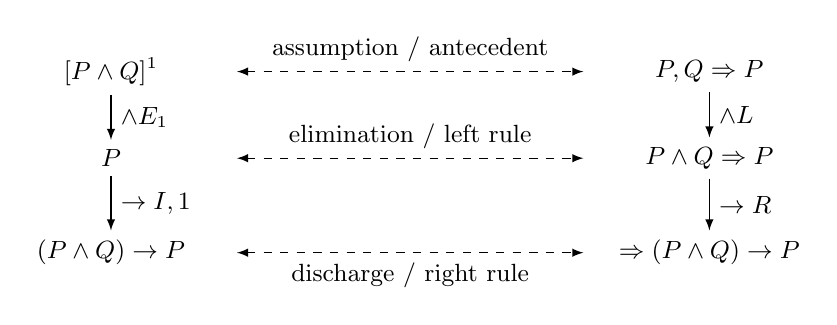
\begin{tikzpicture}[font=\small,>=latex]
  \node (nda) at (-3.8,2.3) {$[P\land Q]^1$};
  \node (ndp) at (-3.8,1.2) {$P$};
  \node (ndi) at (-3.8,0) {$(P\land Q)\to P$};
  \draw[->] (nda) -- node[right] {$\land E_1$} (ndp);
  \draw[->] (ndp) -- node[right] {$\to I,1$} (ndi);

  \node (lki) at (3.8,2.3) {$P,Q\Rightarrow P$};
  \node (lka) at (3.8,1.2) {$P\land Q\Rightarrow P$};
  \node (lkr) at (3.8,0) {$\Rightarrow(P\land Q)\to P$};
  \draw[->] (lki) -- node[right] {$\land L$} (lka);
  \draw[->] (lka) -- node[right] {$\to R$} (lkr);

  \draw[<->,dashed] (-2.2,2.3) -- node[above] {assumption / antecedent} (2.2,2.3);
  \draw[<->,dashed] (-2.2,1.2) -- node[above] {elimination / left rule} (2.2,1.2);
  \draw[<->,dashed] (-2.2,0) -- node[below] {discharge / right rule} (2.2,0);
\end{tikzpicture}
\caption{One natural-deduction/\(\mathsf{LK}\) correspondence.
The arrows exhibit this example's matching steps; they do not claim a
step-for-step equivalence for arbitrary proofs.}
\label{fig:p02-nd-lk-correspondence}
\end{figure}

\section{Analytic tableaux}
\label{sec:p02-analytic-tableaux}

\begin{hbdefinition}{def:p02-cpl-tableau}{Tableau}
For finite \(\Gamma\subseteq\mathsf{Fm}_{\mathsf{CPL}}\), a
\emph{tableau rooted at \(\Gamma\)} is a finite tree of retained branch
lists.  They are built under registry sheet
\hyperref[sheet:tableaux-cpl]{\texttt{sheet:tableaux-cpl}}.  Applying an
expansion appends formulas and marks the principal occurrence as expanded;
it never consumes that occurrence.  A branch is \emph{closed} when it
contains \(\bottom\) or contains both \(\alpha\) and \(\neg\alpha\), and
\emph{open} otherwise.  It is \emph{saturated} when every expandable
occurrence on it is marked.  These marks are metalinguistic bookkeeping, not
formula symbols.  A tableau is closed exactly when every branch is closed.

The root branch lists each member of \(\Gamma\) once; consequence and
validity are tested by rooting at \(\Gamma\cup\{\neg\varphi\}\) and at
\(\{\neg\varphi\}\).  The expandable formulas, expansion steps and finished
tableaux are fixed in
\cref{def:p02-w02-p02-014-input,def:p02-w02-p02-014-expandable}.
\end{hbdefinition}

\begin{hbtheorem}{thm:p02-tableau-adequacy}{proved=annex:p02-w02-p02-014-tableau-adequacy}{Tableau adequacy}
Let \(\Gamma\) be a finite set of propositional formulas.  Every closed
tableau rooted at \(\Gamma\) certifies that \(\Gamma\) is unsatisfiable.
Exhaustively expanding unmarked expandable occurrences
(\cref{def:p02-w02-p02-014-expandable}) terminates in a finite finished
tableau, each of whose branches is closed or saturated.  From any open saturated branch \(B\), define a valuation
by assigning a propositional variable \(p\) true exactly when \(p\) occurs
on \(B\) (and false otherwise).  This branch valuation satisfies every
formula on \(B\), hence every member of \(\Gamma\).  Consequently an
exhaustively expanded saturated tableau has an open branch
exactly when \(\Gamma\) is satisfiable, and it is closed exactly when
\(\Gamma\) is unsatisfiable.
\end{hbtheorem}

\begin{figure}[htbp]
\centering
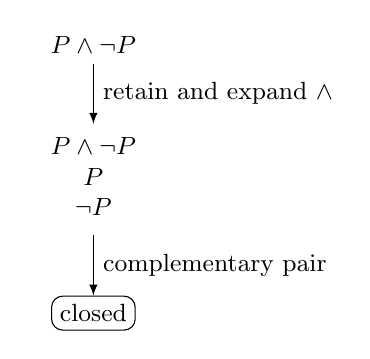
\begin{tikzpicture}[font=\small,>=latex]
  \node (root) at (0,2.7) {$P\land\neg P$};
  \node (expanded) at (0,1.0)
    {$\begin{array}{c}P\land\neg P\\ P\\ \neg P\end{array}$};
  \node[draw,rounded corners,inner sep=3pt] (closed) at (0,-0.7) {closed};
  \draw[->] (root) -- node[right] {retain and expand \(\land\)} (expanded);
  \draw[->] (expanded) -- node[right] {complementary pair} (closed);
\end{tikzpicture}
\caption{A closed propositional tableau for
\(\{P\land\neg P\}\).  The root formula remains on the branch
after expansion; the last node records closure rather than replacing any
formula.}
\label{fig:p02-closed-tableau}
\end{figure}

\begin{landscape}
\section{Proof-system comparison}
\label{sec:p02-proof-system-comparison}

\begingroup\scriptsize\setlength{\tabcolsep}{3pt}
\begin{longtable}{@{}p{.72in}p{1.20in}p{1.80in}p{1.45in}p{1.70in}@{}}
\caption{Classical propositional proof systems side by side.}
\label{tab:p02-proof-systems}\\
\toprule
System & Registry home & Derivation object and rule families & Adequacy form & Proof-search behavior \\ \midrule
\endfirsthead
\caption[]{Classical propositional proof systems side by side (continued)}\\
\toprule
System & Registry home & Derivation object and rule families & Adequacy form & Proof-search behavior \\ \midrule
\endhead
\midrule\multicolumn{5}{r}{\emph{continued on next page}}\\
\endfoot
\endlastfoot
Hilbert & \hyperref[sheet:hilbert-cpl]{\texttt{sheet:hilbert-cpl}} & Finite formula sequence; axiom schemas and one inference rule & Sound and complete after the displayed translation, Theorem~\ref{thm:p02-calculi-derivability-equivalence} & Compact for metatheory; little goal-directed structure \\
Natural deduction & \hyperref[sheet:nd-cpl]{\texttt{sheet:nd-cpl}} & Rooted formula tree; introduction, elimination, and nonvacuous discharge & Sound and complete, same theorem & Goal-directed introductions; eliminations may create detours \\
\(\mathsf{LK}\) & \hyperref[sheet:lk]{\texttt{sheet:lk}} & Tree of finite-multiset sequents; initial, structural, logical, and Cut inferences & Sound and complete, same theorem & Backward search becomes analytic when Cut is excluded; normalization is Part~7 \\
Tableau & \hyperref[sheet:tableaux-cpl]{\texttt{sheet:tableaux-cpl}} & Retained branch lists with linear and splitting expansions & Exhaustive saturated tableau closed iff unsatisfiable; open branch yields a model & Direct refutation search with branch closure and countermodel extraction \\
Resolution & \hyperref[sheet:resolution-cpl]{\texttt{sheet:resolution-cpl}} & Clause sequence generated from inputs by binary resolution & Sound by the inline theorem in \cref{sec:prop-metatheory-04}; finite refutational completeness is \cref{thm:prop-resolution-complete}, with the arbitrary-set extension stated in \cref{rem:resolution-finiteness} & Saturation/search depends strongly on clause choice and redundancy control \\
\bottomrule
\end{longtable}
\endgroup
\end{landscape}

\section{Propositional rejection and proofs of nonvalidity}
\label{sec:p02-classical-rejection}

A refutation calculus can certify that a formula fails to be a theorem
without proving its negation. This is a different task from deriving a
contradiction from assumptions. The classical construction below uses
the antiaxiom and rejection operations recorded in
\cite[\S1, pp.~68--69]{Citkin2013JankovRefutation}. The general signed
metastatement notation occurs in that paper's Definitions~4.1--4.3.

\begin{hbdefinition}{def:p02-crf-judgments}{Assertion and rejection are metalinguistic judgments}
Use the \(\{\neg,\to\}\) language and finite Hilbert derivations of
\cref{def:p02-hilbert-derivation}. Boolean valuations take values
\(0,1\), with negation exchanging these values and material implication
false exactly at antecedent one and consequent zero.
Write \(\vdash A\) when that
calculus derives \(A\) with no open assumptions. Its classical adequacy
is the empty-premise instance of
\cref{thm:p02-calculi-derivability-equivalence}.
Write \(\dashv A\) for the distinct formal rejection judgment defined
below. It is not the object formula \(\neg A\).
The source's \(A^{+}\) and \(A^{-}\) are signed metastatements:
their intended meanings are, respectively, that \(A\) belongs and does
not belong to the indicated logic. In this classical construction they
correspond to \(\vdash A\) and \(\dashv A\). The superscripts do not
extend the formula grammar.
\end{hbdefinition}

\begin{hbdefinition}{def:p02-crf-derivation}{The classical rejection calculus}
Fix one propositional variable \(p\). Its judgment \(\dashv p\) is
the antiaxiom. A rejection derivation is a finite sequence of judgments.
A positive line must be accompanied by a closed Hilbert derivation;
a negative line is the antiaxiom or follows from earlier lines by the
rejection modus-tollens or reverse-substitution operation on the sheet.
A substitution \(\sigma\) maps variables to formulas and extends
homomorphically through \(\neg,\to\). Replacement is simultaneous:
it does not apply \(\sigma\) again inside the inserted formulas.
Positive proofs, substitutions, and earlier-line references are part
of the certificate, not unrecorded oracle answers.
\end{hbdefinition}

\calculussheet{sheet:p02-classical-rejection}{Classical propositional rejection}{Closed positive CPC proofs; negative judgments certify nonvalidity; negation remains an object-language connective; no equality or open-hypothesis rejection rule.}
\hbrule{rule:p02-crf-antiaxiom}{Antiaxiom}{}{\dashv p}{p is the fixed propositional variable of the rejection calculus.}
\hbrule{rule:p02-crf-mt}{Rejection modus tollens}{\vdash(A\to B)\qquad\dashv B}{\dashv A}{The positive premise has a closed proof in the specified sound classical calculus.}
\hbrule{rule:p02-crf-rs}{Reverse substitution}{\dashv\sigma(A)}{\dashv A}{sigma is a simultaneous uniform substitution of formulas for variables.}


The positive premise of rejection modus tollens must be a theorem,
not a formula derived under hypotheses. Reverse substitution removes
a substitution from a rejected instance; it does not substitute freely
into an arbitrary rejection. The consequences of reversing either
restriction are exhibited below.

\begin{hblemma}{thm:p02-crf-substitution}{proved=annex:p02.crf.substitution}{Truth under simultaneous substitution}
For any Boolean valuation \(w\), let \(v(x)=w(\sigma(x))\) on
variables. Then \(w(\sigma(A))=v(A)\) for every formula \(A\).
Consequently a countervaluation of \(\sigma(A)\) supplies a
countervaluation of \(A\); a theorem \(A\) has only theorem
substitution instances.
\end{hblemma}

\begin{hbtheorem}{thm:p02-crf-soundness}{proved=annex:p02.crf.soundness}{Every rejection has a countervaluation}
If a rejection derivation ends in \(\dashv A\), some Boolean
valuation makes \(A\) false. In particular, no classically valid
formula is rejected, and no formula is both asserted and rejected
by these calculi.
\end{hbtheorem}

\subsection{Turning a countervaluation into a rejection certificate}
\label{sec:p02-crf-certificate}

\begin{hbdefinition}{def:p02-crf-constants}{Formula constants for the substitution construction}
Put \(T=(p\to p)\) and \(F=\neg(p\to p)\).
Every Boolean valuation gives \(T\) value one and \(F\) value zero.
Citkin's introductory construction instead uses the formulas
\((p\to p)\) and \((p\land\neg p)\). The latter has the same
constant-zero truth function as \(F\); \(F\) keeps the present
construction within the stated primitive Hilbert language.
For a countervaluation \(v\) of \(A\), define \(\sigma_v(x)=T\)
if \(v(x)=1\), and \(\sigma_v(x)=F\) if \(v(x)=0\).
The distinguished variable \(p\) need not be fresh because this
substitution is simultaneous and both inserted formulas are constant
as truth functions.
\end{hbdefinition}

\begin{hbtheorem}{thm:p02-crf-completeness}{proved=annex:p02.crf.completeness}{Every classically invalid formula has a rejection derivation}
If \(A\) has a countervaluation \(v\), then
\(\sigma_v(A)\to p\) is a classical theorem. Its closed positive
proof, the antiaxiom \(\dashv p\), rejection modus tollens, and
reverse substitution form a rejection derivation of \(A\).
Thus \(\dashv A\) is derivable exactly when \(A\) is not valid.
The proof supplies the substitution identity for every valuation and
explains the finite positive-proof obligation.
\end{hbtheorem}

\begin{hbexample}{def:p02-crf-example}{A complete rejection of an implication}
For \(A=(q\to r)\), choose \(v(q)=1,v(r)=0\).
The corresponding instance is \(\sigma_v(A)=(T\to F)\).
There is a closed positive proof of \((T\to F)\to p\).
Together with \(\dashv p\), the sheet's two rejection operations
give \(\dashv(T\to F)\) and then \(\dashv(q\to r)\).
The annex gives the actual Hilbert lines under the single temporary
assumption \(T\to F\), then discharges it by the proved deduction
theorem. The certificate does not assert \(\neg(q\to r)\): the
valuation \(q=0,r=0\) makes \(q\to r\) true.
\end{hbexample}

\begin{hbtheorem}{thm:p02-crf-polarity}{proved=annex:p02.crf.polarity}{Rejection, negation, and the three truth-function cases}
Rejection of \(A\) means \((\exists v)\,v(A)=0\), whereas assertion
of \(\neg A\) means \((\forall v)\,v(A)=0\).
A tautology is asserted and not rejected. A contradiction is rejected
and its negation is asserted. For a contingent formula, both it and
its negation are rejected, while neither is asserted. These two
rejections may use different countervaluations.
Forward substitution on arbitrary negative judgments and use of a
hypothesis-dependent positive implication in rejection modus tollens
would each allow rejection of a tautology.
\end{hbtheorem}

\begin{hbwarning}{def:p02-crf-wrong-directions}{Two unsound rule changes}
Forward negative substitution would send \(\dashv p\) to
\(\dashv(p\to p)\) by substituting \(p\to p\) for \(p\).
Also, under the hypothesis \(q\), the formula \(T\to q\) is
derivable. Combining that hypothesis-dependent derivation with
\(\dashv q\) as if it were a closed theorem would reject \(T\).
The calculus permits neither change. A rejected formula is not an
assumption that is false in every model under discussion.
\end{hbwarning}

\begin{hbmethod}{def:p02-crf-procedure}{Finding and checking an assertion or rejection certificate}
List the finitely many variables occurring in the input \(A\), and
evaluate \(A\) on all their Boolean assignments. If all results are
one, search the effectively enumerable closed Hilbert proofs for a
proof of \(A\). If some result is zero, construct \(\sigma_v\)
from that assignment, search for a closed proof of
\(\sigma_v(A)\to p\), and append the two rejection steps.
Check every positive proof against its actual axiom schemas and
modus-ponens indices; check each negative step against the literal
sheet and the displayed substitution. Finite truth-table search finds
the appropriate branch. Completeness guarantees termination of its
subsequent positive-proof search, but gives no efficient proof-size
bound.
\end{hbmethod}

\begin{hbtheorem}{thm:p02-crf-procedure}{proved=annex:p02.crf.procedure}{Termination and the meaning of the checked output}
With the countable effectively encoded propositional language and
the stated sound and complete positive calculus, the procedure
terminates on every formula. A checked positive output establishes
validity; a checked negative output establishes nonvalidity.
It does not conflate a short truth-table counterexample, a potentially
long syntactic rejection certificate, and a derivation of a negation.
\end{hbtheorem}

\begin{proofboundary}{def:p02-crf-scope}{The classical theorem does not transfer unchanged to other logics}
The completeness construction uses Boolean formula constants and
classical positive completeness. In intermediate or modal logics,
rejection may require different antiaxioms and characteristic formulas.
The signed framework alone neither proves their refutation
completeness nor turns the absence of a discovered proof into a
rejection certificate \cite[\S1 and Definitions~4.1--4.3]{Citkin2013JankovRefutation}.
\end{proofboundary}

\begin{inheritedrestorationscope}{SRC-02451-02544}
\chapter{Soundness, Completeness, Compactness, and Resolution}
\label{ch:prop-metatheory}

\section{Soundness}
\label{sec:prop-metatheory-01}

\begin{theorem}[Soundness of classical propositional natural deduction]
\label{thm:prop-nd-soundness}
For all \(\Gamma\subseteq\Fm_{\CPL}\) and
\(\varphi\in\Fm_{\CPL}\),
\[
 \Gamma\derives_{\ND_{\CPL}}\varphi
 \quad\Longrightarrow\quad
 \Gamma\entails\varphi.
\]
\end{theorem}
\begin{proof}
Induct on the construction of the derivation.  The induction statement is
stronger than the theorem: every valuation satisfying all open assumptions of
a subderivation satisfies its conclusion.

An assumption case is immediate.  The conjunction introduction and
elimination cases, disjunction introduction cases, implication elimination
case, negation elimination case, and bottom elimination case are each written
out, from the truth clause of the connective concerned, in
\cref{annex:p02-w02b-p02-009-nd-rule-soundness}
(\cref{thm:p02-w02b-p02-009-nd-rule-soundness}).  For \(\lor E\), let \(v\) satisfy the
open assumptions of the conclusion.  It satisfies \(\varphi\lor\psi\), so it
satisfies \(\varphi\) or \(\psi\).  In the first case the induction hypothesis
for the left subsidiary derivation gives \(v\entails\chi\); in the second case
the right subsidiary derivation gives the same conclusion.

For \(\to I\), let \(v\) satisfy the open assumptions.  If
\(v\notentails\varphi\), then \(v\entails\varphi\to\psi\).  If
\(v\entails\varphi\), it satisfies every open assumption of the subsidiary
derivation, so the induction hypothesis gives \(v\entails\psi\).  Thus again
\(v\entails\varphi\to\psi\).  The \(\neg I\) case is analogous: if
\(v\entails\varphi\), the induction hypothesis would give
\(v\entails\bottom\), which is impossible; hence
\(v\entails\neg\varphi\).

For \(\mathsf{RAA}\), suppose \(v\) satisfies the open assumptions
and falsifies \(\varphi\).  Then it satisfies \(\neg\varphi\), so the
induction hypothesis for the subsidiary derivation gives
\(v\entails\bottom\), impossible.  Therefore \(v\entails\varphi\).  Every
rule preserves truth from open assumptions to conclusion, completing the
induction.
\end{proof}

\begin{theorem}[Soundness of the classical propositional sequent calculus]
\label{thm:prop-lk-soundness}
Every sequent derivable in \(\LK_{\CPL}\) is satisfied by every valuation.
\end{theorem}
\begin{proof}
Induct on the sequent derivation, showing that every derivable sequent is
satisfied by every valuation in the sense of the sequent-satisfaction
definition of \cref{sec:prop-deduction-02}.  Both forms of initial sequent
are satisfied by every valuation \(v\).  In an identity sequent
\(\Gamma,\varphi\Rightarrow\varphi,\Delta\), the formula \(\varphi\)
belongs to the support of the antecedent and to the support of the
succedent, so whichever truth value \(v\) gives \(\varphi\), either some
antecedent formula is false under \(v\) or some succedent formula is true
under \(v\).  In a \(\bottom\)-sequent
\(\Gamma,\bottom\Rightarrow\Delta\), the antecedent support contains
\(\bottom\), which is false under \(v\).

For the induction step, suppose toward a contradiction that some valuation
\(v\) does not satisfy the conclusion of a rule each of whose premises is
satisfied by every valuation.  By the sequent-satisfaction definition,
\(v\) makes every formula in the support of the conclusion's antecedent
true and every formula in the support of its succedent false.  For
weakening, the supports of the premise are included in those of the
conclusion, so \(v\) does not satisfy the premise.  For contraction,
premise and conclusion have the same supports, so exactly the same
valuations satisfy both.  For cut, \(v\) makes all formulas in
\(\Gamma,\Sigma\) true and all formulas in \(\Delta,\Pi\) false; because
\(v\) satisfies the left premise, \(\varphi\) is true under \(v\), and
because \(v\) satisfies the right premise, \(\varphi\) is false under
\(v\), which is impossible.

For each logical rule, use the truth clause for the principal connective to
produce a premise that \(v\) does not satisfy.  For example, if \(v\)
does not satisfy the conclusion of \(\land R\), then \(v\) makes every
formula in \(\Gamma\) true, every formula in \(\Delta\) false, and
\(\varphi\land\psi\) false; hence \(\varphi\) or \(\psi\) is false under
\(v\), so \(v\) does not satisfy the corresponding premise.  If \(v\)
does not satisfy the conclusion of \(\to L\), then \(v\) makes
\(\varphi\to\psi\) true.  If \(\varphi\) is false under \(v\), then
\(v\) does not satisfy the left premise; if \(\psi\) is true under
\(v\), then \(v\) does not satisfy the right premise.  The cases for
\(\neg L,\neg R,\land L,\lor L,\lor R,\to R\) are each written out in
\cref{annex:p02-w02b-p02-009-lk-rule-soundness}
(\cref{thm:p02-w02b-p02-009-lk-rule-soundness}), together with every other
rule case.  Thus every rule whose
premises are satisfied by every valuation has a conclusion satisfied by
every valuation, completing the induction.
\end{proof}


\end{inheritedrestorationscope}

\begin{inheritedrestorationscope}{SRC-02545-02664}
\section{Maximal consistent sets}
\label{sec:prop-metatheory-02}

\begin{definition}[Consistency]
A set \(\Gamma\subseteq\Fm_{\CPL}\) is \emph{consistent} iff
\(\Gamma\notderives_{\ND_{\CPL}}\bottom\).
\end{definition}

\begin{definition}[Maximal consistent set]
A \emph{maximal consistent set} is a consistent set
\(\Delta\subseteq\Fm_{\CPL}\) such that
\(\Delta\cup\set{\varphi}\) is inconsistent for every
\(\varphi\notin\Delta\).
\end{definition}

\begin{lemma}[Closure properties]
\label{lem:prop-mcs}
If \(\Delta\) is maximal consistent, then:
\begin{enumerate}
  \item if \(\Delta\derives_{\ND_{\CPL}}\varphi\), then
        \(\varphi\in\Delta\);
  \item exactly one of \(\varphi\) and \(\neg\varphi\) belongs to
        \(\Delta\);
  \item \(\varphi\land\psi\in\Delta\) iff
        \(\varphi\in\Delta\) and \(\psi\in\Delta\);
  \item \(\varphi\lor\psi\in\Delta\) iff
        \(\varphi\in\Delta\) or \(\psi\in\Delta\); and
  \item \(\varphi\to\psi\in\Delta\) iff
        \(\varphi\notin\Delta\) or \(\psi\in\Delta\).
\end{enumerate}
\end{lemma}
\begin{proof}
For 1, suppose \(\Delta\derives\varphi\) but \(\varphi\notin\Delta\).
Maximality makes \(\Delta\cup\set{\varphi}\) inconsistent.  Substitute the
derivation of \(\varphi\) for every open use of the added assumption by
\cref{lem:nd-substitution}; this yields a derivation of \(\bottom\) from
\(\Delta\), contrary to consistency.

The two formulas in 2 cannot both belong to \(\Delta\), by \(\neg E\).  If
\(\varphi\notin\Delta\), maximality yields a derivation \(D\) of
\(\bottom\) whose open assumptions lie in \(\Delta\cup\set{\varphi}\).
Because \(\Delta\) is consistent, at least one open occurrence of
\(\varphi\) remains in \(D\).  Mark all open occurrences of \(\varphi\) in
\(D\) with a common fresh label \(i\), by the merging relabeling of the
derivation definition, and apply \(\neg I\) with label \(i\) at the root,
discharging every such occurrence, to obtain
\(\Delta\derives\neg\varphi\); then 1 gives \(\neg\varphi\in\Delta\).
This proves 2.

For 3, conjunction elimination proves the forward implication and conjunction
introduction proves the reverse implication, using 1.  For 4, disjunction
introduction proves the reverse implication.  If
\(\varphi\lor\psi\in\Delta\) while neither disjunct belongs to \(\Delta\),
then 2 gives \(\neg\varphi,\neg\psi\in\Delta\).  Disjunction elimination,
using each negation to derive \(\bottom\) in its corresponding branch, derives
\(\bottom\) from \(\Delta\), a contradiction.

For 5, if \(\varphi\to\psi\in\Delta\) and \(\varphi\in\Delta\), implication
elimination and 1 give \(\psi\in\Delta\).  Conversely, if
\(\psi\in\Delta\), assume \(\varphi\) with label \(i\) and take \(\psi\)
as an open assumption; \(\land I\) gives \(\varphi\land\psi\), and
\(\land E_2\) gives \(\psi\); then \(\to I\) discharges the single open
occurrence marked \(i\), concluding \(\varphi\to\psi\) with open
assumptions in \(\Delta\).  The discharged occurrence is genuinely
present, and only displayed rules occur.  If \(\varphi\notin\Delta\), then
\(\neg\varphi\in\Delta\) by 2; from an assumed \(\varphi\), derive
\(\bottom\), then \(\psi\), and discharge the assumption, which occurs
open in that derivation.  In either case 1
places \(\varphi\to\psi\) in \(\Delta\).
\end{proof}

\begin{lemma}[Lindenbaum lemma]
\label{lem:prop-lindenbaum}
Every consistent subset of \(\Fm_{\CPL}\) is contained in a maximal
consistent set.
\end{lemma}
\begin{proof}
The set \(\Fm_{\CPL}\) is countable; enumerate it as
\(\varphi_0,\varphi_1,\ldots\).  Starting with a consistent set
\(\Gamma_0=\Gamma\), define
\[
 \Gamma_{n+1}=
 \begin{cases}
   \Gamma_n\cup\set{\varphi_n},&
     \text{if this set is consistent},\\
   \Gamma_n,&\text{otherwise}.
 \end{cases}
\]
Let \(\Delta=\bigcup_{n\in\N}\Gamma_n\).  If \(\Delta\) were inconsistent,
a finite derivation of \(\bottom\) would use only finitely many assumptions,
all lying in some \(\Gamma_n\), contradicting its consistency.  Thus
\(\Delta\) is consistent.  If \(\varphi_n\notin\Delta\), it was rejected at
stage \(n+1\), so \(\Gamma_n\cup\set{\varphi_n}\), and hence
\(\Delta\cup\set{\varphi_n}\), is inconsistent.  Therefore \(\Delta\) is
maximal consistent.
\end{proof}

\begin{lemma}[Truth lemma]
\label{lem:prop-truth}
Let \(\Delta\) be maximal consistent and define a valuation \(v_\Delta\) by
\[
  v_\Delta(p_n)=\True\quad\text{iff}\quad p_n\in\Delta.
\]
Then, for every propositional formula \(\varphi\),
\[
  v_\Delta\entails\varphi
  \quad\text{iff}\quad
  \varphi\in\Delta.
\]
\end{lemma}
\begin{proof}
Proceed by structural induction.  The variable case is the definition of
\(v_\Delta\), and \(\bottom\notin\Delta\) by consistency.  The negation case
uses \cref{lem:prop-mcs}(2) and the truth clause for \(\neg\).  The
conjunction, disjunction, and implication cases use respectively clauses 3,
4, and 5 of that lemma together with the corresponding recursive truth
clauses.  These are all constructors in the grammar, so the induction is
complete.
\end{proof}


\end{inheritedrestorationscope}

\begin{inheritedrestorationscope}{SRC-02665-02809}
\section{Completeness and compactness}
\label{sec:prop-metatheory-03}

\begin{theorem}[Strong completeness of classical propositional natural deduction]
\label{thm:prop-completeness}
For every \(\Gamma\subseteq\Fm_{\CPL}\) and every
\(\varphi\in\Fm_{\CPL}\),
\[
  \Gamma\entails\varphi
  \quad\Longrightarrow\quad
  \Gamma\derives_{\ND_{\CPL}}\varphi.
\]
\end{theorem}
\begin{proof}
We prove the contrapositive.  Suppose
\(\Gamma\notderives_{\ND_{\CPL}}\varphi\).  Then
\(\Gamma\cup\set{\neg\varphi}\) is consistent.  For suppose a derivation
\(D\) of \(\bottom\) has open assumptions in
\(\Gamma\cup\set{\neg\varphi}\).  If no open occurrence of
\(\neg\varphi\) appeared in \(D\), then \(D\) would witness
\(\Gamma\derives_{\ND_{\CPL}}\bottom\), and \(\bottom E\) would give
\(\Gamma\derives_{\ND_{\CPL}}\varphi\), contrary to the supposition.  So
at least one open occurrence remains; mark all open occurrences of
\(\neg\varphi\) in \(D\) with a common fresh label \(i\), by the merging
relabeling of the derivation definition, and apply \(\mathsf{RAA}\) with
label \(i\) at the root, discharging every such occurrence, to obtain
\(\Gamma\derives_{\ND_{\CPL}}\varphi\)---again contrary to the
supposition.  Hence \(\Gamma\cup\set{\neg\varphi}\) is consistent.  By
\cref{lem:prop-lindenbaum}, extend this set to a maximal
consistent set \(\Delta\).  The truth lemma gives
\(v_\Delta\entails\Gamma\) and
\(v_\Delta\entails\neg\varphi\).  Hence
\(v_\Delta\notentails\varphi\), so
\(\Gamma\notentails\varphi\).
\end{proof}

Combining \cref{thm:prop-nd-soundness,thm:prop-completeness} yields
\[
  \Gamma\derives_{\ND_{\CPL}}\varphi
  \quad\text{iff}\quad
  \Gamma\entails\varphi.
\]

\begin{theorem}[Propositional compactness]
\label{thm:prop-compactness}
For every \(\Gamma\subseteq\Fm_{\CPL}\) and every
\(\varphi\in\Fm_{\CPL}\):
\begin{enumerate}
  \item if \(\Gamma\entails\varphi\), then some finite
        \(\Gamma_0\subseteq\Gamma\) satisfies
        \(\Gamma_0\entails\varphi\); and
  \item \(\Gamma\) is satisfiable iff every finite subset of \(\Gamma\) is
        satisfiable.
\end{enumerate}
\end{theorem}
\begin{proof}
If \(\Gamma\entails\varphi\), completeness gives a finite derivation from
\(\Gamma\).  Only finitely many members of \(\Gamma\) occur as open
assumptions; call their set \(\Gamma_0\).  Soundness gives
\(\Gamma_0\entails\varphi\), proving 1.

The forward implication in 2 is immediate.  For the converse, if \(\Gamma\)
were not satisfiable, then \(\Gamma\entails\bottom\).  Clause 1 would give a
finite \(\Gamma_0\subseteq\Gamma\) with
\(\Gamma_0\entails\bottom\), so \(\Gamma_0\) would not be satisfiable.
\end{proof}

\begin{theorem}[Completeness of the sequent calculus]
\label{thm:prop-lk-completeness}
For all finite multisets \(\Gamma,\Delta\) of propositional formulas, the
sequent \(\Gamma\Rightarrow\Delta\) is derivable in \(\LK_{\CPL}\) iff
every valuation making every formula of \(\operatorname{supp}(\Gamma)\)
true makes some formula of \(\operatorname{supp}(\Delta)\) true.
\textit{Status: proof sketch.}
\end{theorem}
\begin{proof}[Proof sketch]
The exact scope is the displayed cut-admitting calculus with finite multiset
contexts.  Left to right is \cref{thm:prop-lk-soundness}, whose semantic
condition on a sequent is exactly the one displayed here.

For right to left, first record the translation subroutine.  Induction on
a \(\ND_{\CPL}\)-derivation translates every introduction rule to the
corresponding right rule, every elimination rule to the corresponding
left rule followed when necessary by cut, and assumption discharge to a
right rule.  Weakening and contraction align the finite contexts.  The
induction establishes that if
\(\Gamma_0\derives_{\ND_{\CPL}}\varphi\) for a finite set \(\Gamma_0\),
then the sequent \(\Gamma_0\Rightarrow\varphi\) is derivable in the
displayed calculus.  The rule-by-rule translation trees, with the exact
count of contractions and weakenings, are
\cref{def:p02-w02b-p02-009-nd-to-lk}, proved correct in
\cref{thm:p02-w02b-p02-009-nd-to-lk}; the translation uses Cut and does not
establish cut elimination, which is
\cref{thm:p02-w02b-p02-009-cut-admissibility}.

Now suppose every valuation making every formula of
\(\operatorname{supp}(\Gamma)\) true makes some formula of
\(\operatorname{supp}(\Delta)\) true, and list
\(\operatorname{supp}(\Delta)=\set{\delta_1,\ldots,\delta_m}\) with
\(m\geq0\).
\begin{enumerate}
  \item Let \(S\) be the set of members of
        \(\operatorname{supp}(\Gamma)\) together with
        \(\neg\delta_1,\ldots,\neg\delta_m\).  A valuation satisfying
        all of \(S\) would make every member of
        \(\operatorname{supp}(\Gamma)\) true, hence some
        \(\delta_j\) true together with \(\neg\delta_j\).  So no
        valuation satisfies \(S\), and \(S\entails\bottom\).
  \item \Cref{thm:prop-completeness} gives
        \(S\derives_{\ND_{\CPL}}\bottom\).  The open assumptions of
        that derivation form a finite subset of \(S\), say
        \(\gamma_1,\ldots,\gamma_k\in\operatorname{supp}(\Gamma)\) and
        \(\neg\delta_{j_1},\ldots,\neg\delta_{j_r}\).  The translation
        subroutine turns it into an \(\LK_{\CPL}\)-derivation of
        \(\gamma_1,\ldots,\gamma_k,
        \neg\delta_{j_1},\ldots,\neg\delta_{j_r}\Rightarrow\bottom\).
  \item Cut with the initial \(\bottom\)-sequent
        \(\bottom\Rightarrow\), the instance of
        \(\Gamma,\bottom\Rightarrow\Delta\) with both contexts empty,
        empties the succedent.
  \item For each \(j\), the sequent
        \(\Rightarrow\delta_j,\neg\delta_j\) is derivable: start from
        the identity sequent \(\delta_j\Rightarrow\delta_j\) and apply
        \(\neg R\).  Cutting it against the current sequent, with cut
        formula \(\neg\delta_j\),
        \[
         \Rule[Cut]{\Rightarrow\delta_j,\neg\delta_j\qquad
          \Gamma',\neg\delta_j\Rightarrow\Pi}
          {\Gamma'\Rightarrow\delta_j,\Pi},
        \]
        moves \(\delta_j\) into the succedent; after \(r\) such cuts
        the derived sequent is
        \(\gamma_1,\ldots,\gamma_k\Rightarrow
        \delta_{j_1},\ldots,\delta_{j_r}\).
  \item Weakening (\(W_L\), \(W_R\)) adds the unused members of
        \(\Gamma\) and \(\Delta\), and contraction (\(C_L\),
        \(C_R\)) merges duplicates, giving exactly the multiset
        sequent \(\Gamma\Rightarrow\Delta\).
\end{enumerate}
When \(m=0\), the hypothesis asserts that no valuation makes every
member of \(\operatorname{supp}(\Gamma)\) true, step 4 performs no cuts,
and the same route derives \(\Gamma\Rightarrow\Delta\) with empty
succedent; an empty \(\Gamma\) is likewise covered.  The route uses cut,
which is primitive in the displayed calculus, and makes no cut-free
claim; no choice principle enters, because the propositional Lindenbaum
lemma runs on a countable enumeration.  The status is a sketch because
the individual translation trees of the subroutine remain omitted.
\end{proof}


\end{inheritedrestorationscope}

%% toc: P2 13 13.4,13.5,13.6,13.7
\section{Tableau soundness and completeness}
\label{sec:p02-w02-p02-014-tableau-metatheory}

A propositional tableau is a search for a valuation satisfying a finite set
of formulas.  The search either closes every branch, which certifies that no
such valuation exists, or ends with an open branch from which a satisfying
valuation can be read off.  This section makes that statement exact for the
calculus of \cref{def:p02-cpl-tableau}, whose rules are displayed on the
calculus sheet \texttt{sheet:\allowbreak tableaux-cpl}, and proves each of its parts: soundness of
closure, termination of exhaustive expansion, the truth lemma for open
saturated branches, and completeness.  Together these results establish every
clause of \cref{thm:p02-tableau-adequacy}.  It then shows why the
termination argument is special to the propositional case and treats the
first-order calculus of \cref{def:p02-fol-tableau}, extended by equality
rules: soundness, extraction of a Herbrand countermodel from an open
saturated (fair) branch, completeness, and a fair systematic procedure that
halts exactly on unsatisfiable inputs.  These results establish every clause
of \cref{thm:p02-fol-tableau-adequacy}.

\emph{Inputs.}  A finite set \(\Gamma\subseteq\mathsf{Fm}_{\mathsf{CPL}}\)
in the language of \cref{sec:prop-syntax-semantics-01}, with primitive
\(\bottom,\neg,\land,\lor,\to\); and, for consequence and validity, one
further formula \(\varphi\).  \emph{Conclusions.}  Either a closed tableau,
which shows that \(\Gamma\) is unsatisfiable (or that \(\Gamma\entails\varphi\)),
or a finished tableau with an open branch together with an explicit valuation
that satisfies \(\Gamma\) (or satisfies \(\Gamma\) and falsifies
\(\varphi\)).  Valuations, satisfaction \(v\entails\chi\), satisfiability,
validity and semantic consequence are those of
\cref{sec:prop-syntax-semantics-02}; \(\widehat v\) is the extension of a
valuation \(v\) to all formulas.  In the first-order part
(\cref{sec:p02-w02-p02-014-fol-calculus,sec:p02-w02-p02-014-fol-herbrand,sec:p02-w02-p02-014-fol-systematic})
the input is a finite set of first-order sentences, with or without
equality, and the conclusion is either a finite closed tableau, which shows
the set unsatisfiable, or an open saturated branch, possibly infinite,
together with a structure built from closed terms that satisfies the set.

\subsection{Input convention, expandable occurrences and finished tableaux}
\label{sec:p02-w02-p02-014-input}

\begin{hbconvention}{def:p02-w02-p02-014-input}{Root branch and the three tests}
Fix a finite set \(\Gamma\) and list it without repetition in a fixed
order as \(\gamma_1,\ldots,\gamma_n\), where \(n=0\) is allowed.  The \emph{root branch}
\(B_\Gamma\) is the list \(\langle\gamma_1,\ldots,\gamma_n\rangle\) with no
expansion marks: it lists each member of \(\Gamma\) exactly once.
\begin{enumerate}
  \item \emph{Satisfiability} of \(\Gamma\) is tested by a tableau rooted at
        \(\Gamma\).
  \item \emph{Consequence} \(\Gamma\entails\varphi\) is tested by a tableau
        rooted at \(\Gamma\cup\{\neg\varphi\}\).  The added formula is
        \(\neg\varphi\) itself, with no simplification even when
        \(\varphi\) is a negation; if \(\neg\varphi\in\Gamma\) already, it is
        listed once.
  \item \emph{Validity} \(\entails\varphi\) is the case
        \(\Gamma=\varnothing\): it is tested by a tableau rooted at
        \(\{\neg\varphi\}\).
\end{enumerate}
\end{hbconvention}

By unique readability (\cref{thm:prop-unique-readability}) every formula of
\(\mathsf{Fm}_{\mathsf{CPL}}\) is a variable \(p\), \(\bottom\), or of the
form \(\neg\chi\) or \((\chi\circ\psi)\) with
\(\circ\in\{\land,\lor,\to\}\), and \(\chi\) in \(\neg\chi\) is again of one of
these forms.  This fixes the following split, on which saturation depends.

\begin{hbdefinition}{def:p02-w02-p02-014-expandable}{Expandable formulas, branches, expansion steps and finished tableaux}
\begin{enumerate}
  \item A formula is \emph{expandable} if it has one of the seven premise
        shapes of the sheet:
        \[
          \varphi\land\psi,\quad \neg(\varphi\land\psi),\quad
          \varphi\lor\psi,\quad \neg(\varphi\lor\psi),\quad
          \varphi\to\psi,\quad \neg(\varphi\to\psi),\quad
          \neg\neg\varphi .
        \]
        Every other formula is \emph{terminal}.  The terminal formulas are
        exactly \(p\), \(\neg p\) (for a variable \(p\)), \(\bottom\) and
        \(\neg\bottom\); the last is the defined verum \(\topv\).  No rule
        has a terminal premise.
  \item Each expandable formula has exactly one rule on the sheet, and that
        rule lists its \emph{alternatives}: one alternative for the
        \emph{linear} shapes and two for the \emph{branching} shapes.
        \[
        \begin{array}{lll}
          \text{premise} & \text{alternatives} & \text{kind}\\ \hline
          \varphi\land\psi & \langle\varphi,\psi\rangle & \text{linear}\\
          \neg(\varphi\lor\psi) & \langle\neg\varphi,\neg\psi\rangle & \text{linear}\\
          \neg(\varphi\to\psi) & \langle\varphi,\neg\psi\rangle & \text{linear}\\
          \neg\neg\varphi & \langle\varphi\rangle & \text{linear}\\
          \neg(\varphi\land\psi) & \langle\neg\varphi\rangle\mid\langle\neg\psi\rangle & \text{branching}\\
          \varphi\lor\psi & \langle\varphi\rangle\mid\langle\psi\rangle & \text{branching}\\
          \varphi\to\psi & \langle\neg\varphi\rangle\mid\langle\psi\rangle & \text{branching}
        \end{array}
        \]
  \item A \emph{branch} is a pair \(B=(\langle\theta_1,\ldots,\theta_m\rangle,M)\)
        of a finite list of formulas and a set \(M\subseteq\{1,\ldots,m\}\)
        of \emph{marked positions}, each holding an expandable formula.  The
        \emph{occurrence} at position \(i\) is the pair \((i,\theta_i)\): two
        positions holding the same formula are two occurrences.  Write
        \(\operatorname{fm}(B)=\{\theta_1,\ldots,\theta_m\}\).  The branch is \emph{closed} if
        \(\bottom\in\operatorname{fm}(B)\) or both \(\chi\in\operatorname{fm}(B)\) and \(\neg\chi\in\operatorname{fm}(B)\) for
        some \(\chi\), and \emph{open} otherwise.
  \item An occurrence at position \(i\) is \emph{expandable on \(B\)} if
        \(B\) is open, \(\theta_i\) is expandable and \(i\notin M\).  An
        \emph{expansion step} at such an occurrence replaces \(B\) by one
        \emph{child} for each alternative \(A\) of \(\theta_i\): the child is
        \((\langle\theta_1,\ldots,\theta_m\rangle\frown A,\;M\cup\{i\})\).
        Nothing is deleted, the new positions are unmarked, and a closed
        branch admits no step.
  \item A \emph{tableau rooted at \(\Gamma\)} is the last member \(T_k\) of an
        \emph{expansion sequence} \(T_0,\ldots,T_k\) of finite lists of
        branches, where \(T_0=\langle B_\Gamma\rangle\) and \(T_{j+1}\)
        replaces one branch of \(T_j\) by its children under one expansion
        step.  It is \emph{closed} if every branch is closed.
  \item An open branch is \emph{saturated} if every position holding an
        expandable formula is marked; terminal occurrences never need a mark.
        A tableau is \emph{finished} if each of its branches is closed or
        saturated.
\end{enumerate}
\end{hbdefinition}

Children keep the positions of their parent, so a position below a split
denotes the same occurrence on every branch descending from the branch where
it was added.  The sheet's instruction to append the conclusions ``on every
open branch through'' an occurrence is therefore a finite run of expansion
steps, one for each open branch that carries that occurrence unmarked, and
every result below applies to it.  The tree drawn in
\cref{fig:p02-closed-tableau} is the picture of an expansion sequence in
which shared initial segments of branches are drawn once.  Saturation is
determinate: whether a branch is saturated depends only on its list and its
mark set.  In particular \(\neg\bottom\) and \(\neg p\) never prevent
saturation, and two occurrences of one expandable formula must each be
expanded.

The termination argument uses a size measure.  For a formula \(\chi\), let
\(\operatorname{sz}(\chi)\) be the number of occurrences of variables,
\(\bottom\) and connectives in \(\chi\) (parentheses are not counted):
\(\operatorname{sz}(p)=\operatorname{sz}(\bottom)=1\),
\(\operatorname{sz}(\neg\chi)=\operatorname{sz}(\chi)+1\) and
\(\operatorname{sz}(\chi\circ\psi)=\operatorname{sz}(\chi)+\operatorname{sz}(\psi)+1\).
For a branch \(B\), put
\[
  \mu(B)\defeq\sum_{\substack{1\leq i\leq m,\ i\notin M,\\
     \theta_i\text{ expandable}}}3^{\operatorname{sz}(\theta_i)},
\]
a sum over positions, so a formula at two unmarked positions counts twice.
For an open branch, \(\mu(B)=0\) exactly
when \(B\) is saturated.  Finally the \emph{branch valuation} of a branch
\(B\) is the valuation \(v_B\) with \(v_B(p)\) true exactly when the variable
\(p\) belongs to \(\operatorname{fm}(B)\).

\subsection{Soundness, termination and the truth lemma}
\label{sec:p02-w02-p02-014-results}

\begin{hblemma}{thm:p02-w02-p02-014-alternatives}{proved=annex:p02-w02-p02-014-alternatives}{Each rule is a semantic case split}
For every expandable formula \(\chi\) and every valuation \(v\),
\(v\entails\chi\) if and only if there is an alternative \(A\) of \(\chi\)
with \(v\entails\alpha\) for every formula \(\alpha\) of \(A\).  Moreover
every formula of every alternative of \(\chi\) has size at most
\(\operatorname{sz}(\chi)-1\), and each alternative has at most two members.
\end{hblemma}

\begin{hblemma}{thm:p02-w02-p02-014-invariants}{proved=annex:p02-w02-p02-014-invariants}{Branch invariants}
Let \(B=(\langle\theta_1,\ldots,\theta_m\rangle,M)\) be a branch of a tableau
rooted at \(\Gamma=\{\gamma_1,\ldots,\gamma_n\}\).
\begin{enumerate}
  \item \(m\geq n\) and \(\theta_\ell=\gamma_\ell\) for \(\ell\leq n\); hence
        \(\Gamma\subseteq\operatorname{fm}(B)\).
  \item For each \(i\in M\), the formula \(\theta_i\) is expandable and some
        alternative \(A\) of \(\theta_i\) satisfies \(A\subseteq\operatorname{fm}(B)\).
\end{enumerate}
\end{hblemma}

\begin{hbtheorem}{thm:p02-w02-p02-014-soundness}{proved=annex:p02-w02-p02-014-soundness}{Soundness of closure}
Let \(\Gamma\) be finite.
\begin{enumerate}
  \item If \(v\entails\operatorname{fm}(B)\) and an expansion step replaces \(B\) by its
        children, then \(v\entails\operatorname{fm}(C)\) for at least one child \(C\).
  \item If \(v\entails\Gamma\), then every tableau rooted at \(\Gamma\) has a
        branch \(B\) with \(v\entails\operatorname{fm}(B)\), and every such branch is open.
  \item If some tableau rooted at \(\Gamma\), finished or not, is closed, then
        \(\Gamma\) is unsatisfiable.
\end{enumerate}
\end{hbtheorem}

\begin{hbtheorem}{thm:p02-w02-p02-014-termination}{proved=annex:p02-w02-p02-014-termination}{Termination of exhaustive expansion}
Let \(\Gamma\) be finite and \(\mu_0\defeq\mu(B_\Gamma)\).
\begin{enumerate}
  \item Every child \(C\) of an expansion step at a branch \(B\) satisfies
        \(\mu(C)<\mu(B)\).
  \item Every expansion sequence \(T_0,\ldots,T_k\) from \(B_\Gamma\) has
        \(k\leq 2^{\mu_0+1}-2\).
  \item A tableau admits an expansion step if and only if it is not finished.
  \item Consequently, expanding expandable occurrences in any order stops
        after at most \(2^{\mu_0+1}-2\) steps, and it stops exactly at a
        finished tableau.  In particular a finished tableau rooted at
        \(\Gamma\) exists.
\end{enumerate}
\end{hbtheorem}

The bound in clause 2 is a crude ceiling that proves termination; it is not
an estimate of the size of a typical tableau.

\begin{hblemma}{thm:p02-w02-p02-014-truth}{proved=annex:p02-w02-p02-014-truth}{Truth lemma for open saturated branches}
Let \(B\) be an open saturated branch of a tableau rooted at a finite set.
Then \(v_B\entails\chi\) for every \(\chi\in\operatorname{fm}(B)\).
\end{hblemma}

\subsection{Completeness, countermodel read-off and decision}
\label{sec:p02-w02-p02-014-completeness}

\begin{hbtheorem}{thm:p02-w02-p02-014-completeness}{proved=annex:p02-w02-p02-014-completeness}{Systematic completeness and countermodel read-off}
Let \(T\) be a finished tableau rooted at a finite set \(\Gamma\).
\begin{enumerate}
  \item \(T\) is closed if and only if \(\Gamma\) is unsatisfiable.
  \item If \(B\) is an open branch of \(T\), then \(v_B\) satisfies every
        formula on \(B\), and in particular \(v_B\entails\Gamma\).
  \item Any two finished tableaux rooted at \(\Gamma\) are either both closed
        or both open, whatever order of expansion produced them.
\end{enumerate}
\end{hbtheorem}

\begin{hbcorollary}{thm:p02-w02-p02-014-consequence}{proved=annex:p02-w02-p02-014-consequence}{Tableau tests for consequence and validity}
Let \(\Gamma\) be finite and \(\varphi\in\mathsf{Fm}_{\mathsf{CPL}}\).
\begin{enumerate}
  \item \(\Gamma\entails\varphi\) if and only if some, equivalently every,
        finished tableau rooted at \(\Gamma\cup\{\neg\varphi\}\) is closed.
  \item If a finished tableau rooted at \(\Gamma\cup\{\neg\varphi\}\) has an
        open branch \(B\), then \(v_B\) is a countervaluation:
        \(v_B\entails\Gamma\) and \(\widehat{v_B}(\varphi)\) is false.
  \item \(\entails\varphi\) if and only if some, equivalently every,
        finished tableau rooted at \(\{\neg\varphi\}\) is closed.
\end{enumerate}
\end{hbcorollary}

\begin{hbmethod}{def:p02-w02-p02-014-procedure}{Systematic tableau procedure}
\emph{Input:} a finite \(\Gamma\subseteq\mathsf{Fm}_{\mathsf{CPL}}\).
\begin{enumerate}
  \item Start with \(T_0=\langle B_\Gamma\rangle\).
  \item While some branch is open and not saturated, take the first such
        branch and the least unmarked position on it holding an expandable
        formula, and perform the expansion step there.
  \item When no step applies, output \emph{unsatisfiable} if every branch is
        closed.  Otherwise take the first open branch \(B\) and output the
        finite set of variables in \(\operatorname{fm}(B)\); it describes \(v_B\).
\end{enumerate}
For \(\Gamma\entails\varphi\) run the procedure on
\(\Gamma\cup\{\neg\varphi\}\) and for \(\entails\varphi\) on
\(\{\neg\varphi\}\): \emph{unsatisfiable} means the consequence (or validity)
holds, and an output valuation is a countervaluation.  Any other fixed rule
for choosing the branch and the position gives the same verdict, by
\cref{thm:p02-w02-p02-014-completeness}(3).
\end{hbmethod}

\begin{hbtheorem}{thm:p02-w02-p02-014-decision}{proved=annex:p02-w02-p02-014-decision}{Propositional tableaux decide by terminating saturation}
For every finite \(\Gamma\), the procedure of
\cref{def:p02-w02-p02-014-procedure} halts after at most
\(2^{\mu(B_\Gamma)+1}-2\) expansion steps.  It outputs \emph{unsatisfiable}
exactly when \(\Gamma\) is unsatisfiable, and any valuation it outputs
satisfies \(\Gamma\).  Hence satisfiability of finite sets of formulas,
validity of formulas, and consequence from finitely many premises are each
decided by an algorithm that halts on every input with the correct answer,
and every negative answer to validity or consequence comes with a
countervaluation.
\end{hbtheorem}

\begin{hbexample}{def:p02-w02-p02-014-example-peirce}{A closed tableau: Peirce's law}
Test \(\entails((P\to Q)\to P)\to P\).  The root branch is
\(\langle\neg(((P\to Q)\to P)\to P)\rangle\).
\begin{enumerate}
  \item Position 1 has the linear shape \(\neg(\varphi\to\psi)\).  Mark it
        and append \((P\to Q)\to P\) (position 2) and \(\neg P\)
        (position 3).
  \item Position 2 has the branching shape \(\varphi\to\psi\).  Mark it.
        The left child appends \(\neg(P\to Q)\) at position 4; the right
        child appends \(P\) at position 4.
  \item The right child contains \(P\) and \(\neg P\) and is closed.
  \item On the left child, position 4 has the shape \(\neg(\varphi\to\psi)\).
        Mark it and append \(P\) and \(\neg Q\).  This child now contains
        \(P\) and \(\neg P\) and is closed.
\end{enumerate}
Both branches are closed, so by \cref{thm:p02-w02-p02-014-consequence} the
formula is valid.  The root measure is
\(\mu_0=3^{\operatorname{sz}(((P\to Q)\to P)\to P)+1}=3^{8}\), and three
steps were used.
\end{hbexample}

\begin{hbexample}{def:p02-w02-p02-014-example-counter}{An open branch and its countervaluation}
Test \(\{P\to Q\}\entails Q\to P\).  The root branch is
\(\langle P\to Q,\ \neg(Q\to P)\rangle\).
\begin{enumerate}
  \item Expand position 2, of shape \(\neg(\varphi\to\psi)\): mark it and
        append \(Q\) (position 3) and \(\neg P\) (position 4).
  \item Expand position 1, of shape \(\varphi\to\psi\): mark it.  The left
        child appends \(\neg P\), the right child appends \(Q\).
\end{enumerate}
The left branch is
\(\langle P\to Q,\neg(Q\to P),Q,\neg P,\neg P\rangle\) with positions 1 and
2 marked.  It is open: \(\bottom\) is not on it, and no formula on it has
its negation on it.  It is saturated, since its unmarked formulas \(Q\) and
\(\neg P\) are terminal.  Its branch valuation makes \(Q\) true and every other variable,
in particular \(P\), false.  It satisfies \(P\to Q\) and falsifies
\(Q\to P\), as \cref{thm:p02-w02-p02-014-consequence}(2) requires, so the
consequence fails.  The right branch is open and saturated as well and gives
the same valuation.  In general different open branches may give different
countervaluations.
\end{hbexample}

\begin{hbwarning}{def:p02-w02-p02-014-unfinished}{An open branch that is not saturated proves nothing}
The truth lemma needs saturation.  The root branch \(\langle P\land\neg
P\rangle\) is open before any expansion, and its branch valuation makes every
variable false; that valuation falsifies \(P\land\neg P\).  Only after the
\(\land\) step does the branch contain \(P\) and \(\neg P\) and close
(\cref{fig:p02-closed-tableau}).  An open branch in an unfinished tableau
therefore supports no conclusion about satisfiability, and a closed branch
alone does not close the tableau: every branch must close.
\end{hbwarning}

\subsection{Why termination is special to the propositional case}
\label{sec:p02-w02-p02-014-fol-contrast}

Termination rests on two facts: an expandable occurrence is expanded at most
once on a branch, and each alternative is smaller than its premise.  The
first-order calculus of \cref{def:p02-fol-tableau} keeps the first fact
for propositional and witness-producing occurrences (its rules are on the
calculus sheet \texttt{sheet:\allowbreak tableaux-fol}), but a universal occurrence, or a negated
existential, stays available at every closed term of the parameter-extended
language \(\mathcal L_{\Gamma}^{*}\) not yet used for it.

\begin{hblemma}{thm:p02-w02-p02-014-fol-no-finite-saturation}{proved=annex:p02-w02-p02-014-fol-no-finite-saturation}{Finite first-order branches with a universal occurrence are not saturated}
Let \(\Gamma\) be a finite set of equality-free sentences and let \(B\) be a
finite open branch of a first-order tableau rooted at \(\Gamma\) in the sense
of \cref{def:p02-fol-tableau}.  If \(B\) contains an occurrence of a formula
\(\forall x\,\varphi\) or \(\neg\exists x\,\varphi\), then \(B\) is not
saturated.  Hence every saturated open branch containing such an occurrence
is infinite.
\end{hblemma}

The rest of this section supplies the first-order metatheory: an exact
bookkeeping for first-order branches, the equality rules, soundness, the
Herbrand truth lemma for open saturated (fair) branches, and the fair
systematic expansion procedure, which semidecides unsatisfiability.

\subsection{First-order tableaux with and without equality}
\label{sec:p02-w02-p02-014-fol-calculus}

Signatures, terms, sentences, structures, satisfaction
\(\mathcal M,s\entails\varphi\) and truth \(\mathcal M\entails\sigma\) are
those of \cref{sec:fol-syntax-semantics-01,sec:fol-semantics-01,sec:fol-semantics-02};
the equality sign is logical and every structure interprets it as identity
on its domain \(\dom\mathcal M\).  For a closed term \(t\), write
\(t^{\mathcal M}\) for its value \(\sem{t}^{\mathcal M}_s\), which does not
depend on the assignment \(s\).  Substitution \(\varphi[t/x]\) is the total
capture-avoiding operation of \cref{sec:fol-syntax-semantics-04}, and
\(c(\varphi)\) is first-order formula complexity, which counts connectives
and quantifiers and is unchanged by substitution
(\cref{lem:substitution-complexity}).

\begin{hbconvention}{def:p02-w02-p02-014-fol-setting}{Root language, parameters and the two calculi}
Let \(\Gamma\) be a finite set of \(\mathcal L\)-sentences.  As in
\cref{def:p02-fol-tableau}, \(\mathcal L_{\Gamma}\) contains exactly the
function and relation symbols occurring in \(\Gamma\), and
\(\mathcal L_{\Gamma}^{*}\) adds pairwise distinct new constant symbols
\(a_0,a_1,\ldots\), the \emph{parameters}, none of which belongs to
\(\mathcal L\).  Let \(\mathrm{CT}_{\Gamma}\) be the set of closed
\(\mathcal L_{\Gamma}^{*}\)-terms.  It is countably infinite, since
\(\mathcal L_{\Gamma}\) is finite and the parameters are infinitely many;
fix a computable enumeration \(t_0,t_1,t_2,\ldots\) in which every member of
\(\mathrm{CT}_{\Gamma}\) occurs.
\begin{enumerate}
  \item The \emph{equality-free calculus} \(\mathsf T\) is the calculus of
        \cref{def:p02-fol-tableau}, whose rules are on the calculus sheet
        \texttt{sheet:\allowbreak tableaux-fol}.  It is used only when no
        member of \(\Gamma\) contains the equality sign.
  \item The \emph{calculus with equality} \(\mathsf T^{=}\) has the rules
        of \(\mathsf T\) together with the two equality rules of
        \cref{def:p02-w02-p02-014-fol-equality}.  Its root \(\Gamma\) may
        contain equations.
\end{enumerate}
By unique readability (\cref{thm:fol-unique-readability}) every
\(\mathcal L_{\Gamma}^{*}\)-sentence has exactly one of the following
\emph{kinds}.  It is \emph{propositional-expandable} if it has one of the
seven premise shapes of \cref{def:p02-w02-p02-014-expandable}, with the
alternatives listed there; a \emph{gamma} sentence if it is
\(\forall x\,\varphi\) or \(\neg\exists x\,\varphi\); a \emph{delta}
sentence if it is \(\exists x\,\varphi\) or \(\neg\forall x\,\varphi\); and
\emph{terminal} otherwise.  The terminal sentences are exactly the atomic
sentences \(R(t_1,\ldots,t_n)\) and \(r=u\), their negations,
\(\bottom\) and \(\neg\bottom\).
\end{hbconvention}

\begin{hbdefinition}{def:p02-w02-p02-014-fol-equality}{Tableau equality rules}
The calculus \(\mathsf T^{=}\) adds two linear rules, with closed terms
\(r,u,t\in\mathrm{CT}_{\Gamma}\).
\begin{enumerate}
  \item \emph{Reflexivity.}  For any \(t\in\mathrm{CT}_{\Gamma}\) not yet
        used for this rule on the branch, append \(t=t\).  The rule has no
        premise; like a gamma rule it stays available at every unused term.
  \item \emph{Replacement.}  Let an occurrence of the equation \(r=u\) and an
        occurrence of an atomic sentence \(\alpha\) lie on the branch, and let
        \(\varphi\) be an atomic \(\mathcal L_{\Gamma}^{*}\)-formula in which
        the variable \(x_0\) occurs exactly once and no other variable
        occurs, with \(\varphi[r/x_0]=\alpha\).  If this triple has not yet
        been used on the branch, append \(\varphi[u/x_0]\).
\end{enumerate}
Replacement therefore rewrites one occurrence of \(r\) in \(\alpha\) to
\(u\), left to right; \(\alpha\) may itself be an equation, and the two
occurrences may coincide.  For given occurrences of \(r=u\) and
\(\alpha\) there are as many choices of \(\varphi\) as there are
occurrences of \(r\) as a subterm of \(\alpha\), which is finitely many.
The rules are the tableau forms of the reflexivity and replacement rules of
the equality calculus of \texttt{sheet:\allowbreak nd-fol}
(\cref{thm:p02-equality-laws}); symmetry and transitivity are not rules here
but are recovered from these two on every saturated branch
(\cref{thm:p02-w02-p02-014-congruence}).
\end{hbdefinition}

\begin{hbdefinition}{def:p02-w02-p02-014-fol-branch}{First-order branches, tasks and steps}
Fix \(\Gamma\) and one of the calculi \(\mathsf T\), \(\mathsf T^{=}\).
\begin{enumerate}
  \item A \emph{branch} is a pair
        \(B=(\langle\theta_1,\theta_2,\ldots\rangle,D)\) of a finite or
        infinite list of \(\mathcal L_{\Gamma}^{*}\)-sentences and a set
        \(D\) of \emph{done tasks}.  Write \(\operatorname{fm}(B)\) for the
        set of sentences on the list.  Closed and open are as in
        \cref{def:p02-w02-p02-014-expandable}: \(B\) is \emph{closed} if
        \(\bottom\in\operatorname{fm}(B)\) or \(\chi,\neg\chi\in\operatorname{fm}(B)\) for some \(\chi\).
  \item The \emph{tasks available on \(B\)} are the following.
        \begin{itemize}
          \item \(\langle i\rangle\), for each position \(i\) holding a
                delta sentence or a propositional-expandable one.
          \item \(\langle i,t\rangle\), for each position \(i\) holding a
                gamma sentence and each \(t\in\mathrm{CT}_{\Gamma}\).
          \item In \(\mathsf T^{=}\) only: \(\langle{=},t\rangle\) for each
                \(t\in\mathrm{CT}_{\Gamma}\); and
                \(\langle i,j,\varphi\rangle\) for positions \(i,j\) such
                that \(\theta_i\) is an equation \(r=u\) and \(\varphi\) is
                as in the replacement rule with
                \(\varphi[r/x_0]=\theta_j\).
        \end{itemize}
  \item An \emph{expansion step} applies to a finite open branch
        \(B=(\langle\theta_1,\ldots,\theta_m\rangle,D)\) at an available task
        \(\tau\notin D\).  It replaces \(B\) by one child
        \((\langle\theta_1,\ldots,\theta_m\rangle\frown A,\;D\cup\{\tau\})\)
        for each alternative \(A\) determined as follows.  For
        \(\langle i\rangle\) with \(\theta_i\) propositional-expandable, the
        alternatives of \(\theta_i\).  For \(\langle i\rangle\) with
        \(\theta_i=\exists x\,\varphi\) or \(\neg\forall x\,\varphi\), the
        single alternative \(\langle\varphi[a/x]\rangle\) or
        \(\langle\neg(\varphi[a/x])\rangle\), where \(a\) is the parameter of
        least index not occurring in \(\theta_1,\ldots,\theta_m\).  For
        \(\langle i,t\rangle\) with \(\theta_i=\forall x\,\varphi\) or
        \(\neg\exists x\,\varphi\), the single alternative
        \(\langle\varphi[t/x]\rangle\) or \(\langle\neg(\varphi[t/x])\rangle\).
        For \(\langle{=},t\rangle\), \(\langle t=t\rangle\); for
        \(\langle i,j,\varphi\rangle\) with \(\theta_i\) the equation \(r=u\),
        \(\langle\varphi[u/x_0]\rangle\).
  \item The \emph{root branch} \(B_\Gamma\) lists the members of \(\Gamma\) once
        each, in a fixed order, with \(D=\varnothing\).  An \emph{expansion
        sequence} is a finite or infinite sequence \(T_0,T_1,\ldots\) of
        finite lists of finite branches with \(T_0=\langle B_\Gamma\rangle\),
        each \(T_{j+1}\) replacing one branch of \(T_j\) by its children under
        one step.  Each branch of \(T_{j+1}\) has a \emph{parent} in \(T_j\):
        the replaced branch, if it is one of its children, and itself
        otherwise.  Iterating parents gives, for \(j\leq j'\), the unique
        \emph{ancestor} in \(T_j\) of each branch of \(T_{j'}\); a branch
        \emph{descends} from its ancestors.  A \emph{finite tableau} rooted at
        \(\Gamma\) is the last member of a finite expansion sequence; it is
        \emph{closed} if all its branches are closed.
  \item A \emph{path} through an infinite expansion sequence is a sequence
        \((B_j)_{j\in\N}\) in which \(B_j\) is a branch of \(T_j\) and
        \(B_j\) is the parent of \(B_{j+1}\).  Its \emph{limit branch}
        \(B_\omega\) has as list the union of the lists of the \(B_j\), each
        of which extends the previous one, and as done set the union of
        their done sets.  The finite branches of the \(T_j\) and the limit
        branches are the branches of the tableau, possibly infinite,
        generated by the sequence.
  \item An open branch \(B\), finite or limit, is \emph{saturated} if every
        task available on \(B\) belongs to \(D\).
\end{enumerate}
\end{hbdefinition}

The tasks make the sheet's records exact.  A done \(\langle i\rangle\) is the
mark of a propositional or delta occurrence.  The done tasks
\(\langle i,t\rangle\) record the terms used for the gamma occurrence at
position \(i\), so a saturated branch has used every \(t_k\) for every gamma
occurrence: saturation in the sense of item 6 is exactly ``fair and
saturated'' in the sense of \cref{def:p02-fol-tableau}.  The freshness
condition is the choice of the least unused parameter in a delta step, and
the instantiation condition is that gamma and reflexivity steps range over
all of \(\mathrm{CT}_{\Gamma}\), not only over terms already on the branch.
As in the propositional case, the sheet's instruction to append conclusions
``on every open branch through'' an occurrence is a finite run of single
steps.  Every instance \(\varphi[t/x]\) appended by a step is again a
sentence, because the premise is a sentence and \(t\) is closed
(\cref{lem:substitution-fv}).  In \(\mathsf T^{=}\) no finite branch is
saturated, since infinitely many reflexivity tasks are available on it.

\begin{hblemma}{thm:p02-w02-p02-014-fol-cases}{proved=annex:p02-w02-p02-014-fol-cases}{First-order rules are sound case splits}
Let \(\mathcal M\) be an \(\mathcal L_{\Gamma}^{*}\)-structure.
\begin{enumerate}
  \item For every propositional-expandable sentence \(\chi\),
        \(\mathcal M\entails\chi\) iff \(\mathcal M\) satisfies every member
        of some alternative of \(\chi\).
  \item If \(\mathcal M\entails\forall x\,\varphi\), then
        \(\mathcal M\entails\varphi[t/x]\) for every
        \(t\in\mathrm{CT}_{\Gamma}\); if
        \(\mathcal M\entails\neg\exists x\,\varphi\), then
        \(\mathcal M\entails\neg(\varphi[t/x])\) for every such \(t\).
  \item Let \(a\) be a parameter that occurs in no member of a set \(X\) of
        sentences.  If \(\mathcal M\entails X\) and
        \(\exists x\,\varphi\in X\), there is a structure \(\mathcal M'\),
        differing from \(\mathcal M\) at most in the interpretation of
        \(a\), with \(\mathcal M'\entails X\cup\{\varphi[a/x]\}\).  The same
        holds with \(\neg\forall x\,\varphi\in X\) and
        \(\neg(\varphi[a/x])\).
  \item \(\mathcal M\entails t=t\); and if \(\mathcal M\entails r=u\) and
        \(\mathcal M\entails\varphi[r/x_0]\) for \(\varphi\) as in the
        replacement rule, then \(\mathcal M\entails\varphi[u/x_0]\).
\end{enumerate}
\end{hblemma}

\begin{hblemma}{thm:p02-w02-p02-014-fol-invariants}{proved=annex:p02-w02-p02-014-fol-invariants}{First-order branch invariants}
Let \(B\) be a finite or limit branch generated from \(B_\Gamma\).  Then
\(\Gamma\subseteq\operatorname{fm}(B)\), and every done task has its conclusion on \(B\):
for \(\langle i\rangle\) with \(\theta_i\) propositional-expandable, some
alternative of \(\theta_i\) is included in \(\operatorname{fm}(B)\); for
\(\langle i\rangle\) with \(\theta_i=\exists x\,\varphi\) (or
\(\neg\forall x\,\varphi\)), \(\varphi[a/x]\in\operatorname{fm}(B)\) (or
\(\neg(\varphi[a/x])\in\operatorname{fm}(B)\)) for some parameter \(a\); for
\(\langle i,t\rangle\), the instance of \(\theta_i\) at \(t\) is in \(\operatorname{fm}(B)\);
for \(\langle{=},t\rangle\), \(t=t\in\operatorname{fm}(B)\); and for
\(\langle i,j,\varphi\rangle\) with \(\theta_i\) the equation \(r=u\),
\(\varphi[u/x_0]\in\operatorname{fm}(B)\).  In \(\mathsf T\), no member of \(\operatorname{fm}(B)\)
contains the equality sign.  A limit branch is open if and only if every
\(B_j\) on its path is open.
\end{hblemma}

\begin{hbtheorem}{thm:p02-w02-p02-014-fol-soundness}{proved=annex:p02-w02-p02-014-fol-soundness}{First-order soundness of closure}
Let \(\Gamma\) be a finite set of \(\mathcal L\)-sentences, equality-free
for \(\mathsf T\).
\begin{enumerate}
  \item If an \(\mathcal L_{\Gamma}^{*}\)-structure satisfies \(\operatorname{fm}(B)\) and
        an expansion step replaces the finite branch \(B\), then some
        \(\mathcal L_{\Gamma}^{*}\)-structure satisfies \(\operatorname{fm}(C)\) for some
        child \(C\).
  \item If \(\Gamma\) has a model, every finite tableau rooted at \(\Gamma\)
        has an open branch.
  \item If some finite tableau rooted at \(\Gamma\) is closed, then
        \(\Gamma\) is unsatisfiable.
\end{enumerate}
\end{hbtheorem}

\subsection{Hintikka sets and the Herbrand truth lemma}
\label{sec:p02-w02-p02-014-fol-herbrand}

\begin{hbdefinition}{def:p02-w02-p02-014-hintikka}{Hintikka sets and their quotient Herbrand structures}
A set \(H\) of \(\mathcal L_{\Gamma}^{*}\)-sentences is a \emph{Hintikka
set} if:
\begin{enumerate}
  \item[(H0)] \(\bottom\notin H\), and no \(\chi\) has both \(\chi\in H\)
        and \(\neg\chi\in H\);
  \item[(H1)] if \(\chi\in H\) is propositional-expandable, every member of
        some alternative of \(\chi\) is in \(H\);
  \item[(H2)] if \(\forall x\,\varphi\in H\), then \(\varphi[t/x]\in H\), and
        if \(\neg\exists x\,\varphi\in H\), then \(\neg(\varphi[t/x])\in H\),
        for every \(t\in\mathrm{CT}_{\Gamma}\);
  \item[(H3)] if \(\exists x\,\varphi\in H\), then \(\varphi[t/x]\in H\), and
        if \(\neg\forall x\,\varphi\in H\), then \(\neg(\varphi[t/x])\in H\),
        for some \(t\in\mathrm{CT}_{\Gamma}\);
  \item[(H4)] if some member of \(H\) contains the equality sign, then
        \(t=t\in H\) for every \(t\in\mathrm{CT}_{\Gamma}\), and
        \(\varphi[u/x_0]\in H\) whenever \(r=u\in H\) and
        \(\varphi[r/x_0]\in H\) for \(\varphi\) as in the replacement rule.
\end{enumerate}
\(H\) is \emph{equality-free} if none of its members contains the equality
sign.  For a Hintikka set \(H\), put \(r\sim_H u\) iff \(r\) and \(u\) are
the same term or \(r=u\in H\).  The \emph{quotient Herbrand structure}
\(\mathcal M_H\) has domain \(\mathrm{CT}_{\Gamma}/{\sim_H}\), whose
members are the classes \([t]\); it interprets \(f\) by
\(f^{\mathcal M_H}([t_1],\ldots,[t_n])=[f(t_1,\ldots,t_n)]\) and \(R\) by
\(R^{\mathcal M_H}=\{([t_1],\ldots,[t_n]):R(t_1,\ldots,t_n)\in H\}\).
\end{hbdefinition}

\begin{hblemma}{thm:p02-w02-p02-014-congruence}{proved=annex:p02-w02-p02-014-congruence}{The branch equality is a congruence}
Let \(H\) be a Hintikka set.  Then \(\sim_H\) is an equivalence relation on
\(\mathrm{CT}_{\Gamma}\); if \(t_i\sim_H u_i\) for \(1\leq i\leq n\), then
\(f(t_1,\ldots,t_n)\sim_H f(u_1,\ldots,u_n)\), and
\(R(t_1,\ldots,t_n)\in H\) implies \(R(u_1,\ldots,u_n)\in H\).  Hence
\(\mathcal M_H\) is well defined, \(t^{\mathcal M_H}=[t]\) for every
\(t\in\mathrm{CT}_{\Gamma}\), and
\(([t_1],\ldots,[t_n])\in R^{\mathcal M_H}\) iff
\(R(t_1,\ldots,t_n)\in H\).  If \(H\) is equality-free, \(\sim_H\) is
identity, each class is a singleton, and \(\mathcal M_H\) is, after
identifying \([t]\) with \(t\), the Herbrand structure
\(\mathcal M_{B^{+}_{\mathrm{at}}}\) of
\cref{thm:p02-fol-tableau-adequacy} with \(B^{+}_{\mathrm{at}}\) the atomic
members of \(H\).
\end{hblemma}

\begin{hblemma}{thm:p02-w02-p02-014-herbrand-truth}{proved=annex:p02-w02-p02-014-herbrand-truth}{Herbrand truth lemma}
If \(H\) is a Hintikka set, then \(\mathcal M_H\entails\chi\) for every
\(\chi\in H\).
\end{hblemma}

\begin{hblemma}{thm:p02-w02-p02-014-saturated-hintikka}{proved=annex:p02-w02-p02-014-saturated-hintikka}{Open saturated branches are Hintikka sets}
If \(B\) is an open saturated branch, finite or limit, of a tableau rooted at
\(\Gamma\) in \(\mathsf T\) or \(\mathsf T^{=}\), then \(\operatorname{fm}(B)\) is a Hintikka
set, and in \(\mathsf T\) it is equality-free.
\end{hblemma}

\begin{hbtheorem}{thm:p02-w02-p02-014-fol-extraction}{proved=annex:p02-w02-p02-014-fol-extraction}{Countermodel extraction from an open saturated branch}
Let \(B\) be an open saturated branch, finite or limit, of a tableau rooted
at a finite set \(\Gamma\) of \(\mathcal L\)-sentences in \(\mathsf T\) or
\(\mathsf T^{=}\), and let \(H=\operatorname{fm}(B)\).  Then
\(\mathcal M_H\entails\chi\) for every \(\chi\) on \(B\).  Its reduct
\(\mathcal M_H\restriction\mathcal L_{\Gamma}\) satisfies \(\Gamma\), and
interpreting the symbols of \(\mathcal L\) outside \(\mathcal L_{\Gamma}\)
arbitrarily on the same domain gives an \(\mathcal L\)-structure satisfying
\(\Gamma\).  In \(\mathsf T\), \(\mathcal M_H\) is the Herbrand structure
\(\mathcal M_{B^{+}_{\mathrm{at}}}\) of
\cref{thm:p02-fol-tableau-adequacy}.
\end{hbtheorem}

\subsection{Fair systematic expansion and semidecision}
\label{sec:p02-w02-p02-014-fol-systematic}

An arbitrary order of expansion can starve a gamma occurrence forever
(\cref{def:p02-w02-p02-014-fol-unfair}).  The following procedure performs
at each stage a finite batch of tasks that grows with the stage, so every
task available on a surviving branch is eventually performed.

\begin{hbmethod}{def:p02-w02-p02-014-fol-procedure}{Fair systematic expansion}
\emph{Input:} a finite set \(\Gamma\) of \(\mathcal L\)-sentences, with the
calculus \(\mathsf T\) if \(\Gamma\) is equality-free and \(\mathsf T^{=}\)
otherwise, and the enumeration \(t_0,t_1,\ldots\) of
\cref{def:p02-w02-p02-014-fol-setting}.  Let \(T^{(0)}=\langle
B_\Gamma\rangle\).  At stage \(n=0,1,2,\ldots\), with current finite tableau
\(T^{(n)}\):
\begin{enumerate}
  \item If every branch of \(T^{(n)}\) is closed, halt with output
        \emph{unsatisfiable} and the closed tableau \(T^{(n)}\).
  \item If some branch of \(T^{(n)}\) is finite, open and saturated, halt
        with output \emph{satisfiable} and that branch.
  \item Otherwise, for each branch \(B\) of \(T^{(n)}\) that is open, with
        list length \(m_B\), form the finite list \(W_n(B)\) of the
        following tasks, in a fixed order: \(\langle i\rangle\) for
        \(i\leq m_B\) holding a propositional-expandable or delta sentence;
        \(\langle i,t_k\rangle\) for \(i\leq m_B\) holding a gamma sentence
        and \(k\leq n\); and, in \(\mathsf T^{=}\), \(\langle{=},t_k\rangle\)
        for \(k\leq n\) and every replacement task \(\langle
        i,j,\varphi\rangle\) with \(i,j\leq m_B\).  Taking the tasks of
        \(W_n(B)\) in order, perform the expansion step at the task on every
        open branch that descends from \(B\) and does not yet have that task
        done, until none remains.  The resulting tableau is
        \(T^{(n+1)}\).
\end{enumerate}
\end{hbmethod}

\begin{hbtheorem}{thm:p02-w02-p02-014-fol-semidecision}{proved=annex:p02-w02-p02-014-fol-semidecision}{Fair systematic expansion semidecides unsatisfiability}
Let \(\Gamma\) be a finite set of \(\mathcal L\)-sentences and run
\cref{def:p02-w02-p02-014-fol-procedure}.
\begin{enumerate}
  \item Each stage performs finitely many expansion steps, and the steps of
        all stages, in order, form an expansion sequence from \(B_\Gamma\).
  \item \emph{Infinite branch construction.}  If the procedure does not
        halt, there is a path \((B_j)_{j\in\N}\) through this expansion
        sequence whose limit branch \(B_\omega\) is open and saturated, and
        so fair; \(B_\omega\) is infinite.
  \item The procedure halts with output \emph{unsatisfiable} if and only if
        \(\Gamma\) is unsatisfiable, and then it outputs a finite closed
        tableau rooted at \(\Gamma\).  It halts with output
        \emph{satisfiable} only if \(\Gamma\) is satisfiable, and when
        \(\Gamma\) is satisfiable and it does not halt, the model
        \(\mathcal M_{\operatorname{fm}(B_\omega)}\) of clause 2 satisfies \(\Gamma\) by
        \cref{thm:p02-w02-p02-014-fol-extraction}.
  \item Consequently the procedure is an algorithm that halts with output
        \emph{unsatisfiable} on exactly the unsatisfiable finite sets of
        sentences.
\end{enumerate}
\end{hbtheorem}

\begin{hbcorollary}{thm:p02-w02-p02-014-fol-completeness}{proved=annex:p02-w02-p02-014-fol-completeness}{First-order tableau completeness, consequence and validity}
Let \(\Gamma\) be a finite set of \(\mathcal L\)-sentences and \(\psi\) an
\(\mathcal L\)-sentence; use \(\mathsf T\) when the sentences involved are
equality-free and \(\mathsf T^{=}\) otherwise.
\begin{enumerate}
  \item \(\Gamma\) is unsatisfiable if and only if some finite closed
        tableau rooted at \(\Gamma\) exists.
  \item \(\Gamma\entails\psi\) if and only if some finite closed tableau
        rooted at \(\Gamma\cup\{\neg\psi\}\) exists, and \(\entails\psi\) if
        and only if some finite closed tableau rooted at \(\{\neg\psi\}\)
        exists.
  \item If an open saturated branch \(B\) of a tableau rooted at
        \(\Gamma\cup\{\neg\psi\}\) exists, the expansion of
        \(\mathcal M_{\operatorname{fm}(B)}\restriction\mathcal L_{\Gamma\cup\{\neg\psi\}}\) of
        \cref{thm:p02-w02-p02-014-fol-extraction} is a countermodel:
        it satisfies \(\Gamma\) and falsifies \(\psi\).
\end{enumerate}
\end{hbcorollary}

\begin{hbexample}{def:p02-w02-p02-014-fol-example-closed}{A closed first-order tableau}
In \(\mathsf T\), test the consequence
\[
  \{\forall x(Px\to Qx),\ \exists x\,Px\}\entails\exists x\,Qx .
\]
The root branch is
\(\langle\forall x(Px\to Qx),\ \exists x\,Px,\ \neg\exists x\,Qx\rangle\);
\(\mathcal L_{\Gamma}\) has no function symbols, so the closed terms are the
parameters.
\begin{enumerate}
  \item Task \(\langle 2\rangle\), a delta step: the least parameter not on
        the branch is \(a_0\); append \(Pa_0\) (position 4).
  \item Task \(\langle 1,a_0\rangle\), a gamma step: append
        \(Pa_0\to Qa_0\) (position 5).
  \item Task \(\langle 3,a_0\rangle\), a gamma step: append \(\neg Qa_0\)
        (position 6).
  \item Task \(\langle 5\rangle\), branching: the left child appends
        \(\neg Pa_0\) and closes against position 4; the right child
        appends \(Qa_0\) and closes against position 6.
\end{enumerate}
The finite tableau is closed, so the consequence holds by
\cref{thm:p02-w02-p02-014-fol-completeness}(2).  The gamma steps were made at
the parameter that the delta step introduced.  The systematic procedure
need not choose this order, but fairness guarantees that it performs both
gamma tasks at \(a_0\) by stage \(k\), where \(a_0\) is \(t_k\) in the
enumeration.
\end{hbexample}

\begin{hbexample}{def:p02-w02-p02-014-fol-example-eq}{Equality steps}
Let \(c,d\) be constant symbols and \(\Gamma=\{c=d,\ Pd,\ \neg Pc\}\), in
\(\mathsf T^{=}\).
\begin{enumerate}
  \item Task \(\langle{=},c\rangle\): append \(c=c\) (position 4).
  \item Task \(\langle 1,4,\varphi\rangle\) with \(\varphi\) the formula
        \(x_0=c\): since \(\varphi[c/x_0]\) is \(c=c\), append
        \(\varphi[d/x_0]\), that is \(d=c\) (position 5).
  \item Task \(\langle 5,2,Px_0\rangle\): since \((Px_0)[d/x_0]\) is \(Pd\),
        append \(Pc\) (position 6).  The branch now contains \(Pc\) and
        \(\neg Pc\) and closes.
\end{enumerate}
Replacement rewrites only from left to right, so symmetry had to be
obtained from reflexivity first, exactly as in the proof of
\cref{thm:p02-w02-p02-014-congruence}.
\end{hbexample}

\begin{hbexample}{def:p02-w02-p02-014-fol-example-open}{A finite saturated open branch and its Herbrand countermodel}
Let \(c\) be a constant symbol and \(\Gamma=\{\exists x\,Px,\ \neg Pc\}\), in
\(\mathsf T\).  At stage 0 the only task is \(\langle 1\rangle\); the least
parameter not on the branch is \(a_0\), and the step appends \(Pa_0\).  At
stage 1 the branch \(\langle\exists x\,Px,\neg Pc,Pa_0\rangle\) is open and,
as it carries no gamma sentence, saturated, so the procedure halts with
output \emph{satisfiable}.  The structure \(\mathcal M_H\) has domain the
closed terms \(c,a_0,a_1,\ldots\) and interprets \(P\) as \(\{a_0\}\); its
reduct to \(\{P,c\}\) satisfies \(\exists x\,Px\) and \(\neg Pc\).
\end{hbexample}

\begin{hbexample}{def:p02-w02-p02-014-fol-example}{A satisfiable first-order root with no finite finished tableau}
Let \(\Gamma=\{\forall x\,Px\}\) with \(P\) a unary relation symbol.  Then
\(\mathcal L_{\Gamma}\) has no constant or function symbol, so the closed
\(\mathcal L_{\Gamma}^{*}\)-terms are exactly the parameters \(a_0,a_1,\ldots\).
The root occurrence is retained on every branch, so by
\cref{thm:p02-w02-p02-014-fol-no-finite-saturation} no finite tableau rooted
at \(\Gamma\) has a saturated open branch, and no finite tableau rooted at
\(\Gamma\) is closed, since \(\Gamma\) is true in a one-element structure
in which \(P\) holds of that element
(\cref{thm:p02-w02-p02-014-fol-soundness}(3)).  The procedure of
\cref{def:p02-w02-p02-014-fol-procedure} therefore never halts.  Stage \(n\)
appends \(Pt_n\); the limit branch
\(\langle\forall x\,Px,Pt_0,Pt_1,\ldots\rangle\) is open, saturated
and infinite, and
\(\mathcal M_H\) has domain \(\{a_0,a_1,\ldots\}\) with \(P\) true of every
element.  So the propositional stopping rule ``expand until every branch is
closed or saturated'' never stops here.
\end{hbexample}

\begin{hbwarning}{def:p02-w02-p02-014-fol-unfair}{An unfair branch is not a countermodel}
Let \(\Gamma=\{\forall x\,Px,\ \forall x\,\neg Px\}\), which is
unsatisfiable.  Expanding only the first occurrence, at
\(a_0,a_1,a_2,\ldots\) in turn, is a legal infinite expansion sequence whose
single limit branch \(\langle\forall x\,Px,\forall x\,\neg
Px,Pa_0,Pa_1,\ldots\rangle\) is open.  It is not saturated: no task
\(\langle 2,t\rangle\) is done.  The Herbrand structure whose relations are given
by the atoms on the branch makes \(P\) true of every parameter and falsifies
\(\forall x\,\neg Px\).  The systematic
procedure performs \(\langle 2,t_0\rangle\) at stage 0 and closes the
tableau.  Openness without fairness supports no conclusion.
\end{hbwarning}

\begin{hbwarning}{def:p02-w02-p02-014-fol-freshness}{The delta parameter must be new}
The set \(\Gamma\) of
\cref{def:p02-w02-p02-014-fol-example-open}, with members \(\exists x\,Px\)
and \(\neg Pc\), is satisfiable.  A delta
step that used \(c\) instead of a new parameter would append \(Pc\) and close
the only branch, a closed tableau for a satisfiable set.  The proof of
\cref{thm:p02-w02-p02-014-fol-cases}(3) uses exactly that the parameter
does not occur on the branch.
\end{hbwarning}

\begin{proofboundary}{def:p02-w02-p02-014-fol-boundary}{Decision versus semidecision}
For a finite propositional input, \cref{thm:p02-w02-p02-014-decision}
gives a procedure that always halts and answers both ways.  For first-order
input, \cref{thm:p02-w02-p02-014-fol-semidecision} gives a procedure that
halts on every unsatisfiable input with a finite closed tableau, and that may
run forever on a satisfiable one, as in
\cref{def:p02-w02-p02-014-fol-example}; on a satisfiable input it builds an
infinite fair branch whose quotient Herbrand structure is a model.  The
difference is not an artefact of the procedure: by
\cref{thm:fol-validity-undecidable}, whose status is cited there, first-order
validity is not decidable, and \(\psi\) is valid exactly when \(\{\neg\psi\}\)
is unsatisfiable, so no algorithm halts on every input with the correct
satisfiability verdict.  This section proves the semidecision, the infinite
branch construction and the failure of the propositional termination
argument (\cref{thm:p02-w02-p02-014-fol-no-finite-saturation}); the
undecidability theorem is used only for this concluding remark.
\end{proofboundary}

\subsection{Relationships and sources}
\label{sec:p02-w02-p02-014-relations}

The tableau verdict agrees with the other classical propositional calculi:
by \cref{thm:p02-w02-p02-014-consequence} and the derivability equivalence
\cref{thm:p02-calculi-derivability-equivalence}, whose proof is cited there,
a finite consequence has a
closed tableau exactly when it is derivable in each of the calculi compared
in \cref{tab:p02-proof-systems}.  Resolution
(\cref{thm:prop-resolution-complete}) is also a refutation method, but it
saturates a clause set instead of splitting branches and does not keep a
branch from which a valuation is read.  A finished tableau for
\(\{\neg\varphi\}\) with an open branch is a semantic certificate that
\(\varphi\) is not valid; for formulas of the \(\{\neg,\to\}\) language, the rejection calculus of
\cref{sec:p02-classical-rejection} certifies the same fact by a syntactic
derivation of the rejection judgment, which is a different kind of object.

In the first-order case the Herbrand truth lemma plays the role of the truth
lemma for maximal consistent sets with witnesses
(\cref{lem:fol-truth}): both build a model from closed terms modulo a
provable or listed equality.  The difference is that a Hintikka set need not
be maximal, and the tableau constructs it by a fair search instead of by an
enumeration of all sentences.  The first-order results of this section prove
every clause of \cref{thm:p02-fol-tableau-adequacy} and extend it to roots
with equality.

The unsigned uniform rule format on the sheets is attributed there to
\cite{Smullyan1968}.  The definitions and proofs in this section, including
the task bookkeeping, the tableau equality rules derived from the
natural-deduction equality rules, and the staged fair procedure, are written
directly for the retained-occurrence formats of the calculus sheets
\texttt{sheet:\allowbreak tableaux-cpl} and \texttt{sheet:\allowbreak
tableaux-fol}; they are not a transcription of a published proof.

\begin{inheritedrestorationscope}{SRC-02810-02914}
\section{Propositional resolution}
\label{sec:prop-metatheory-04}

The clause object in this section is exactly the finite set defined in
\cref{sec:prop-syntax-semantics-04}.  A valuation satisfies a clause set \(S\) iff it
satisfies every \(C\in S\), so the set is interpreted conjunctively.  The
complement of \(p\) is \(\neg p\), and the complement of \(\neg p\) is
\(p\).  A clause containing both a literal and its complement is
\emph{tautological}; its formula interpretation is valid, so deleting it from
a clause set preserves the satisfying valuations of that set.

\begin{definition}[Resolvent]
Let \(E\) and \(F\) be clauses, let \(L\in E\), and let its complement
\(\overline L\) belong to \(F\).  Their \emph{resolvent on \(L\)} is the
clause
\[
  (E\setminus\set{L})\cup(F\setminus\set{\overline L}).
\]
A \emph{resolution derivation} from a clause set \(S\) is a finite sequence
whose members are clauses in \(S\) or resolvents of earlier members.
\end{definition}

\begin{theorem}[Soundness of propositional resolution]
Every valuation satisfying both parent clauses satisfies their resolvent.
Consequently, deriving the empty clause proves that the initial clause set is
not satisfiable.
\end{theorem}
\begin{proof}
Let \(E,F\) be the parents and let
\(R=(E\setminus\set{L})\cup(F\setminus\set{\overline L})\).  Suppose a
valuation falsifies \(R\).  It therefore falsifies every nonpivot literal in
both parents.  To satisfy \(E\), it must satisfy \(L\); to satisfy \(F\), it
must satisfy \(\overline L\).  No valuation satisfies complementary
literals.  Therefore no valuation can satisfy both parents while falsifying
the resolvent.  Induction on a resolution derivation preserves satisfaction.
The empty clause is false under every valuation.
\end{proof}

\begin{theorem}[Refutational completeness of propositional resolution]
\label{thm:prop-resolution-complete}
Let \(S\) be a finite set of clauses.  Then \(S\) is not satisfiable
iff the empty clause has a resolution derivation from \(S\).
\end{theorem}
\begin{proof}
Soundness proves the reverse implication.  For the forward implication,
delete tautological clauses.  Induct on the number of variables occurring in
\(S\).  If there are no variables, an unsatisfiable clause set contains the
empty clause.

Choose a variable \(p\).  Form \(S_p\) from all clauses not containing
\(p\) or \(\neg p\), together with every non-tautological resolvent on
\(p\) of a clause containing \(p\) and a clause containing \(\neg p\).  We claim that
\(S\) is satisfiable iff \(S_p\) is satisfiable.  Restricting a valuation
satisfying \(S\) to the other variables satisfies all retained clauses and all
resolvents by soundness.  Conversely, let \(w\) satisfy \(S_p\).  A clause
\(\set{p}\cup A\), where \(p\notin A\), whose remainder \(A\) is false
under \(w\) requires \(p=\True\); a clause
\(\set{\neg p}\cup B\), where \(\neg p\notin B\), whose remainder \(B\)
is false requires \(p=\False\).  Both requirements cannot occur:
otherwise the resolvent \(A\cup B\) on \(p\) would be false under
\(w\); being false under \(w\), it contains no complementary pair of
literals, so it is not tautological, belongs to \(S_p\), and contradicts
the assumption that \(w\) satisfies \(S_p\).  Choose either
permitted value for \(p\).  The resulting extension satisfies \(S\), proving
the claim.

If \(S\) is not satisfiable, neither is \(S_p\).  It contains fewer variables,
so the induction hypothesis gives a resolution derivation of the empty clause
from \(S_p\).  Every noninitial clause of \(S_p\) is itself a resolvent of
clauses in \(S\).  Splicing those one-step derivations into the derivation from
\(S_p\) gives a resolution derivation from \(S\).
\end{proof}

\begin{remark}[Attribution and scope of the finiteness hypothesis]
\label{rem:resolution-finiteness}
The variable-elimination step in the proof of
\cref{thm:prop-resolution-complete}---passing from \(S\) to \(S_p\) and
discarding the variable \(p\)---is the elimination rule of Davis and
Putnam \cite{DavisPutnam1960}.  The finiteness hypothesis on \(S\) is
consumed by the induction, not by the result: an infinite clause set may
contain infinitely many variables, and the induction on the number of
variables then has no measure to decrease.  The restriction is removed by
propositional compactness.  Suppose an arbitrary clause set \(S\) is not
satisfiable.  A valuation satisfies a clause \(C\) iff it satisfies the
formula \(\operatorname{form}_{\CPL}(C)\) of
\cref{sec:prop-syntax-semantics-04}, so the formula set
\(\set{\operatorname{form}_{\CPL}(C):C\in S}\) is not satisfiable, and
\cref{thm:prop-compactness} gives a finite subset of it that is not
satisfiable.  Selecting for each of its finitely many members one clause
of \(S\) interpreting it yields a finite \(S_0\subseteq S\) that is not
satisfiable.  \Cref{thm:prop-resolution-complete} applied to \(S_0\)
gives a resolution derivation of the empty clause from \(S_0\), and every
resolution derivation from \(S_0\) is one from \(S\).  Since the
soundness theorem above is stated without finiteness of the clause set,
the equivalence of \cref{thm:prop-resolution-complete} therefore holds
for every clause set, finite or not.
\end{remark}

Resolution is a refutation calculus: it derives the empty clause from an
unsatisfiable clause set.  Conversion to conjunctive normal form and
resolution must therefore be kept distinct.  The former supplies clauses; the
latter derives clauses.  The original resolution method is due to Robinson
\cite{Robinson1965}; normal-form transformations and their preservation
properties are treated systematically in \cite{BaazEglyLeitsch2001}.


\end{inheritedrestorationscope}

\begin{inheritedrestorationscope}{SRC-02915-02932}
\section{Common errors}
\label{sec:prop-metatheory-05}

\begin{warning}[Propositional ambiguity]
The following replacements are invalid unless separately justified:
\begin{enumerate}
  \item replacing \(\varphi\to\psi\) by \(\psi\to\varphi\);
  \item treating \(\varphi\lor\psi\) as exclusive;
  \item inferring either disjunct from a disjunction;
  \item inferring \(\varphi\) from \(\varphi\to\psi\) and \(\psi\);
  \item using a truth table for some variables while ignoring another variable
        occurring in the formula;
  \item citing soundness in the completeness direction; and
  \item calling a clause set satisfiable because resolution search has not yet
        found the empty clause.
\end{enumerate}
\end{warning}


\end{inheritedrestorationscope}

\begin{inheritedrestorationscope}{SRC-02933-03021}
\section{Exercises}
\label{sec:prop-metatheory-06}

\begin{exercise}
\label{ex:prop-metatheory-01}
Parse
\(\neg P\land Q\to R\lor S\) using the declared precedence and associativity
conventions.  Restore every parenthesis required by the grammar and list all
subformulas.  Draw its syntax tree
(\cref{def:p02-w02-p02-044-syntax-tree}) and compare it with the worked parse
in \cref{fig:p02-w02-p02-044-syntax-tree}.
\end{exercise}

\begin{exercise}
\label{ex:prop-metatheory-02}
Prove by structural induction that, in the syntax tree of every formula, the
number of leaves---occurrences of propositional variables or \(\bottom\)---is
one greater than the number of binary-connective occurrences
(\cref{def:p02-w02-p02-044-syntax-tree}).  The tree in
\cref{fig:p02-w02-p02-044-syntax-tree} is one instance, with five leaves and
four binary-connective nodes.
\end{exercise}

\begin{exercise}
\label{ex:prop-metatheory-03}
Construct a countervaluation to
\(P\to Q,Q\entails P\).  Explain why this refutes semantic consequence but
does not by itself inspect any derivation.
\end{exercise}

\begin{exercise}
\label{ex:prop-metatheory-04}
Translate ``The process terminates only if either the input is finite or the
search is bounded, but not both.''  Supply a key and state whether ``or'' is
inclusive before adding the final restriction.
\end{exercise}

\begin{exercise}
\label{ex:prop-metatheory-05}
Find conjunctive and disjunctive normal forms for
\((P\to Q)\land(Q\to R)\).  Verify both by a truth table.
\end{exercise}

\begin{exercise}
\label{ex:prop-metatheory-06}
Give a \(\ND_{\CPL}\)-derivation of
\((P\to R)\to((Q\to R)\to(P\lor Q\to R))\).
Mark every discharged assumption.
\end{exercise}

\begin{exercise}
\label{ex:prop-metatheory-07}
Derive \(\neg(P\land\neg P)\) without using \(\mathsf{RAA}\).  Then
identify the discharging rule used in place of \(\mathsf{RAA}\), and explain
why every rule in the derivation is available in both classical and
intuitionistic natural deduction.
\end{exercise}

\begin{exercise}
\label{ex:prop-metatheory-08}
Give a cut-free \(\LK_{\CPL}\)-derivation of
\(P\to Q, Q\to R\Rightarrow P\to R\).
\end{exercise}

\begin{exercise}
\label{ex:prop-metatheory-09}
Prove that logical equivalence is an equivalence relation and a congruence for
every primitive connective.
\end{exercise}

\begin{exercise}
\label{ex:prop-metatheory-10}
Use the maximal-consistent-set construction to find a countervaluation to a
chosen underivable formula.  Show explicitly how membership in the
set determines the valuation.
\end{exercise}

\begin{exercise}
\label{ex:prop-metatheory-11}
Convert
\[
 (P\lor Q)\land(\neg P\lor R)\land(\neg Q\lor R)\land\neg R
\]
to a clause set and give a resolution refutation.
\end{exercise}

\begin{exercise}
\label{ex:prop-metatheory-12}
Show that deleting a tautological clause preserves the set of satisfying
valuations.  Show by example that deleting a clause that some valuation
satisfies, but that is not tautological, can change the set of valuations
satisfying the clause set.
\end{exercise}


\end{inheritedrestorationscope}

%% parts/p02/propositional-metatheory-supplement.tex --- retained editorial additions
\section*{Editorial supplement to the restored chapter}
\addcontentsline{toc}{section}{Editorial supplement to the restored chapter}
\noindent\textit{Reader note.} The following separately attributed editorial
additions are retained after the exact source chapter so that the inherited
order and bytes remain intact.  The Boolean Prime Ideal calibration belongs
with \cref{sec:prop-metatheory-03}, and the resolution-refutation DAG belongs
with \cref{sec:prop-metatheory-04}.  These additions do not replace exact
inherited statements, supply aliases for unlabeled source results, or change
any source or review status.

\begin{hbdefinition}{def:p02-arbitrary-prop-language}{Finitary propositional language on an arbitrary set}
For an arbitrary set \(P\), \(\operatorname{Form}(P)\) is the least set
containing \(P\) and closed under the fixed finitary connectives. A valuation
is a total function \(v:P\to\{0,1\}\), extended by structural recursion. The
word ``arbitrary'' is necessary because the source completeness proof
enumerates a countable alphabet. This stands as a set-indexed syntax/semantics,
differs only in cardinality rather than formula arity, and is used in the
choice-calibrated completeness theorem.  Write
\(\Gamma\vdash_{\mathsf{CPL}(P)}\varphi\) when there is a finite
discharge-labelled natural-deduction tree using exactly the inherited
\(\mathsf{ND}_{\mathsf{CPL}}\) rules, with formula metavariables ranging over
\(\operatorname{Form}(P)\) and every open assumption belonging to \(\Gamma\).
This is a \(P\)-parameterized proof relation, not a new rule system; it is used
in the theorem and its Lindenbaum quotient.
\index{propositional language!arbitrary alphabet}
\end{hbdefinition}

\begin{hbtheorem}{thm:p02-arbitrary-prop-compactness-bpi}{cited=HowardRubin1998}{Boolean Prime Ideal Theorem and unrestricted propositional compactness}
Working over \(\mathsf{ZF}\), the Boolean Prime Ideal Theorem (equivalently,
the Ultrafilter Lemma of Definition~\ref{def:ultrafilter-lemma}) is equivalent
to the following scheme: for every set \(P\) of propositional variables and
every set \(\Gamma\subseteq\operatorname{Form}(P)\), if each finite subset
of \(\Gamma\) is satisfiable, then \(\Gamma\) is satisfiable.
\end{hbtheorem}

See also \cite{Jech1973Choice,PaseauLeek2022} for the choice-principle and
logical formulations of this equivalence.  Theorem~\ref{thm:prop-compactness}
is weaker in set-theoretic strength: its fixed countable alphabet supports the
explicit enumeration used in Lemma~\ref{lem:prop-lindenbaum}, with no appeal
to a Boolean prime ideal.  The arbitrary-language theorem does not silently
upgrade that narrower source proof.

The Boolean-algebra/filter extension construction and both directions of
the unrestricted compactness equivalence are given in
\cref{thm:p01-bpi-equivalence,thm:p01-bpi-propositional-compactness}.

\begin{hbtheorem}{thm:p02-arbitrary-prop-completeness}{cited=HowardRubin1998}{Choice-calibrated propositional completeness}
Over \(\mathsf{ZF}\), the Boolean Prime Ideal Theorem proves: for every set
\(P\), set \(\Gamma\subseteq\operatorname{Form}(P)\), and formula \(\varphi\),
\[
 \Gamma\models\varphi\quad\Longrightarrow\quad
 \Gamma\vdash_{\mathsf{CPL}(P)}\varphi,
\]
where derivations remain finite and use only finitely many premises. In fact,
the corresponding unrestricted compactness/completeness scheme is equivalent
over \(\mathsf{ZF}\) to the Boolean Prime Ideal Theorem.
\end{hbtheorem}

\noindent\emph{Proof.}
The complete construction, universal property, premise-filter correspondence
and countervaluation proof are supplied in
\cref{sec:p02-free-boolean-completeness,thm:p02-fbc-free,thm:p02-fbc-completeness}.
In outline, form the Lindenbaum Boolean algebra of formulas modulo provable equivalence and
let \(F\) be the proper filter generated by the classes of \(\Gamma\). If
\(\Gamma\nvdash_{\mathsf{CPL}(P)}\varphi\), then \([\varphi]\notin F\). The Boolean Prime Ideal
Theorem extends \(F\) to an ultrafilter avoiding \([\varphi]\). Its
characteristic homomorphism to the two-element Boolean algebra is a valuation
satisfying \(\Gamma\) and falsifying \(\varphi\), contradicting semantic
consequence. For a countable \(P\), the source's explicit enumeration replaces
this ultrafilter extension; no choice principle is silently imported into that
narrower proof.

\section{Propositional duality}
\label{sec:p02-propositional-duality}

\begin{hbdefinition}{def:p02-nnf-dual}{Propositional NNF duality}
Use the metalinguistic NNF presentation
\[
 \alpha ::= L\mid\bottom\mid\topv\mid(\alpha\land\beta)
             \mid(\alpha\lor\beta),
\]
where \(L\) is a literal.  The two units are displayed separately so their
swap is literal even though \(\topv\) is an abbreviation.  Define
\[
\begin{aligned}
 L^{\mathrm d}&=L,&
 \bottom^{\mathrm d}&=\topv,&
 \topv^{\mathrm d}&=\bottom,\\
 (\alpha\land\beta)^{\mathrm d}
   &=\alpha^{\mathrm d}\lor\beta^{\mathrm d},&&
 (\alpha\lor\beta)^{\mathrm d}
   =\alpha^{\mathrm d}\land\beta^{\mathrm d}.
\end{aligned}
\]
This is a metalinguistic operation on NNF presentations, not a new
object-language connective.  Its distinction from negating a formula is
needed to state the CNF--DNF and valid--unsatisfiable correspondences below.
\index{dual formula}\index{duality!propositional}
\end{hbdefinition}

\begin{hbtheorem}{thm:p02-propositional-duality}{proved=annex:p2.1.8}{Duality theorem}
For a valuation \(v\), let \(\bar v\) be the valuation with
\(\bar v(p_n)=\mathbf T\) iff \(v(p_n)=\mathbf F\).  For every NNF
presentation \(\alpha\),
\[
 v\entails\alpha^{\mathrm d}\quad\Longleftrightarrow\quad
 \bar v\not\entails\alpha.
\]
Consequently dualization is an involution, preserves logical equivalence,
exchanges valid formulas with unsatisfiable formulas, maps every CNF formula
to a DNF formula, and maps every DNF formula to a formula logically
equivalent to the CNF formula with the same literal sets.
\end{hbtheorem}

The extension of this theorem to every formula, through the negation normal
form theorem of Section~\ref{sec:prop-syntax-semantics-04}, is
Theorem~\ref{thm:p02-w02-p02-010-arbitrary-duality}; the separation of
dualization from negation is Warning~\ref{def:p02-w02-p02-010-not-negation}.

\begingroup\small
\begin{longtable}{@{}lll@{}}
\caption{The NNF duality dictionary.}
\label{tab:p02-duality}\\
\toprule Object & Dual & Consequence \\
\midrule\endfirsthead
\caption[]{The NNF duality dictionary (continued)}\\
\toprule Object & Dual & Consequence \\
\midrule\endhead
\midrule\multicolumn{3}{r}{\emph{continued on next page}}\\
\endfoot
\endlastfoot
literal \(L\) & \(L\) & complemented valuation reverses its value \\
\(\bottom\) & \(\topv\) & false and true units swap \\
\(\land\) & \(\lor\) & outer conjunction becomes disjunction \\
\(\lor\) & \(\land\) & outer disjunction becomes conjunction \\
CNF & DNF & clauses become conjunctions of literals \\
valid & unsatisfiable & Theorem~\ref{thm:p02-propositional-duality} \\
\bottomrule
\end{longtable}
\endgroup

\section{Interpolation}
\label{sec:p02-prop-interpolation}

\begin{hbdefinition}{def:p02-interpolant}{Craig interpolant, propositional}
If \(\varphi\entails\psi\), a \emph{Craig interpolant} for that consequence
is a formula \(\theta\) such that
\(\varphi\entails\theta\), \(\theta\entails\psi\), and every variable of
\(\theta\) occurs in both \(\varphi\) and \(\psi\).  The name is needed to
distinguish this formula-level witness from an arbitrary intermediate
consequence: its common-vocabulary restriction is the nonredundant clause used
by the theorem and construction below.
\end{hbdefinition}

\begin{hbtheorem}{thm:p02-interpolation}{cited=Craig1957}{Propositional interpolation theorem}
Every semantic consequence \(\varphi\entails\psi\) in classical
propositional logic has a Craig interpolant.
\end{hbtheorem}

\begin{hbmethod}{def:p02-interpolant-truth-table}{Truth-table construction of a propositional interpolant}
Let \(X\) be the finite set of variables common to \(\varphi\) and \(\psi\),
ordered by variable index.
For each assignment \(u:X\to\{0,1\}\) extendible to a valuation satisfying
\(\varphi\), form the complete conjunction of \(X\)-literals describing
\(u\), and disjoin these conjunctions in lexicographic order with \(0<1\).  Empty
conjunction and disjunction use \(\topv\) and \(\bottom\), respectively.
The resulting formula uses only variables from \(X\); its two consequence
clauses are stated separately below so that this derived construction is not
attributed to Craig's original proof.
Part~7 gives the proof-theoretic Maehara construction.
\end{hbmethod}

\begin{hblemma}{thm:p02-interpolant-truth-table-correctness}{proved=annex:p2.3.9}{Correctness of the truth-table interpolant construction}
If \(\varphi\entails\psi\), the output of
Method~\ref{def:p02-interpolant-truth-table} is a Craig interpolant for that
consequence.
\end{hblemma}

\begin{figure}[tp]
\centering
\begin{tikzpicture}[
  clause/.style={draw,rounded corners,inner sep=4pt,font=\small},
  every edge/.style={draw,-{Latex[length=2mm]}},
  level distance=13mm,
  sibling distance=31mm]
\node[clause] (c1) at (0,0) {\(\{P,Q\}\)};
\node[clause] (c2) at (3,0) {\(\{\neg P,R\}\)};
\node[clause] (c4) at (6,0) {\(\{\neg R\}\)};
\node[clause] (c3) at (9,0) {\(\{\neg Q,R\}\)};
\node[clause] (np) at (4.5,-1.5) {\(\{\neg P\}\)};
\node[clause] (nq) at (7.5,-1.5) {\(\{\neg Q\}\)};
\node[clause] (q) at (2.25,-3) {\(\{Q\}\)};
\node[clause] (empty) at (4.875,-4.5) {\(\varnothing\)};
\draw[-{Latex[length=2mm]}] (c2) -- node[left,font=\scriptsize] {\(R\)} (np);
\draw[-{Latex[length=2mm]}] (c4) -- (np);
\draw[-{Latex[length=2mm]}] (c3) -- node[right,font=\scriptsize] {\(R\)} (nq);
\draw[-{Latex[length=2mm]}] (c4) -- (nq);
\draw[-{Latex[length=2mm]}] (c1) -- node[left,font=\scriptsize] {\(P\)} (q);
\draw[-{Latex[length=2mm]}] (np) -- (q);
\draw[-{Latex[length=2mm]}] (q) -- node[left,font=\scriptsize] {\(Q\)} (empty);
\draw[-{Latex[length=2mm]}] (nq) -- (empty);
\end{tikzpicture}
\caption{Resolution-refutation DAG.  Each two-parent merge is an instance of
the rule on \hyperref[sheet:resolution-cpl]{\texttt{resolution-cpl}}; the last node is the empty clause
.}
\label{fig:p02-resolution-dag}
\end{figure}

\section{Decision procedures and complexity}
\label{sec:p02-prop-decision-complexity}

\begin{hbtheorem}{thm:p02-decidability}{proved=annex:p02-w02-p02-018-decidability}{Decidability of classical propositional logic}
There is a terminating algorithm which, on inputs written in the effective
finite representation of Convention~\ref{def:p02-w02-p02-018-input}
(formulas over \(\{p_n:n\in\N\}\), finite premise lists with a
conclusion, and pairs of formulas, as strings over a fixed token alphabet),
decides whether a propositional formula is satisfiable or valid, whether two
formulas are logically equivalent, and whether a finite set \(\Gamma\)
semantically entails a formula \(\varphi\).  The claim concerns finite
inputs in that representation only: it gives no decision procedure for
consequence from an arbitrary infinite theory, and none for an alphabet
without an effective finite representation
(Warning~\ref{def:p02-w02-p02-018-scope}).
\end{hbtheorem}

The inputs of this algorithm are finite encoded strings over coded atoms.
It does not decide satisfiability of infinite premise sets, even
decidable ones over the coded alphabet
(\cref{thm:p02-w02-p02-017-infinite-undecidable}); a set of atoms that
is uncountable or not well-orderable admits no coding at all
(\cref{thm:p02-w02-p02-017-no-coding}); and it does not construct the
valuation that compactness asserts over an arbitrary set of atoms, which
over \(\mathsf{ZF}\) has the strength of the Boolean Prime Ideal
principle (\cref{thm:p02-w02-p02-017-bpi-boundary}).

\begin{hbconvention}{def:p02-complexity-standing}{Complexity standing for propositional decision problems}
A decision problem is here a set \(L\subseteq\{0,1\}^*\).  The class
\(\mathsf P\) consists of the decision problems decided by a deterministic
multitape Turing machine in a number of steps bounded by a polynomial in the
input length.  A polynomial-time
many-one reduction from \(L\) to \(K\) is a polynomial-time computable map
\(f\) such that \(x\in L\) iff \(f(x)\in K\).  The class \(\mathsf{NP}\)
consists of those \(L\) for which some polynomial \(q\) and polynomial-time
predicate \(R\) satisfy, whenever \(n\) is the encoded length of \(x\),
\[
 x\in L\quad\text{iff}\quad
 \text{some string }y\text{ of length at most }q(n)\text{ satisfies }R(x,y).
\]
The class \(\mathsf{coNP}\) consists of complements of \(\mathsf{NP}\)
problems.  For a complexity class \(\mathcal C\), a problem \(K\) is
\(\mathcal C\)-complete under these reductions iff \(K\in\mathcal C\) and
every \(L\in\mathcal C\) has a polynomial-time many-one reduction to \(K\).
These metalinguistic definitions are stated locally because the complexity
claims use the distinctions now; Part~4 supplies the full class ladder.
\index{P@\(\mathsf P\)}\index{NP@\(\mathsf{NP}\)}
\index{coNP@\(\mathsf{coNP}\)}\index{polynomial-time many-one reduction}
\end{hbconvention}

\begin{hbdefinition}{def:p02-sat-taut}{SAT and TAUT}
Write each variable \(p_n\) as the character \texttt{p}, the ordinary binary
digits for \(n\), and the terminator \texttt{;}; use the fully parenthesized formula string;
and encode each character from the resulting finite alphabet by a fixed-width
binary block.  This metalinguistic encoding and its inverse are linear-time
and linearly intertranslatable with ordinary finite-alphabet formula encodings.
\(\mathsf{SAT}\) is the set of encodings of satisfiable formulas, and
\(\mathsf{TAUT}\) is the set of encodings of valid formulas.
Malformed bit strings belong to neither language; syntactic recognition is
linear-time for the fixed encoding.
These metalinguistic abbreviations are needed to distinguish existential
satisfiability from universal validity.  They are not the same decision
problem, although negation relates their complements, and both distinctions
are used in the next two results.
\index{SAT}\index{TAUT}
\end{hbdefinition}

\begin{hbtheorem}{thm:p02-sat-np-complete}{proved=annex:p02-w02-p02-018-sat-np-complete}{SAT NP-completeness}
\(\mathsf{SAT}\) is \(\mathsf{NP}\)-complete under polynomial-time many-one
reductions.
\end{hbtheorem}

Cook's theorem-proving formulation is the historical source
\cite{Cook1971}; the status citation supports the modern formulation above.
Membership, by checking a guessed assignment under the encoding of
Definition~\ref{def:p02-sat-taut}, is
Theorem~\ref{thm:p02-w02-p02-019-sat-in-np}.  Hardness is the Cook--Levin
Theorem~\ref{thm:p04-cook-levin}; its written proof under the Part~4
conventions is Annex~\ref{annex:p02-w02b-p02-015-cook-levin}, which applies
the tableau formula of Theorem~\ref{thm:p02-w02-p02-018-cook-levin}.  Part~9
presents the same tableau method in the form of Cook's paper
(\cref{sec:p09-presentation-n-c-026}).

\begin{hbcorollary}{thm:p02-taut-conp-complete}{proved=annex:p02-w02-p02-018-taut-conp-complete}{TAUT is coNP-complete}
\(\mathsf{TAUT}\) is \(\mathsf{coNP}\)-complete under polynomial-time
many-one reductions.
\end{hbcorollary}

The preceding classification does not settle whether
\(\mathsf P=\mathsf{NP}\) or \(\mathsf{NP}=\mathsf{coNP}\).  Part~4 locates
these open equalities in the complexity-class ladder
(\cref{def:p04-complexity-convention,thm:p04-cook-levin}); Part~12 treats SAT
solvers as algorithms rather than as complexity-class collapses
(\cref{sec:p12-sat-and-certificates}).  Satisfiability is distinguished from
validity and from logical equivalence in
Warning~\ref{def:p02-w02-p02-019-sat-vs-equivalence}.

\begin{hbdefinition}{def:p02-tractable-classes}{Horn, dual-Horn, 2-CNF, and XOR instances}
A clause is \emph{Horn} when it has at most one positive literal and
\emph{dual-Horn} when it has at most one negative literal.  A clause set is
\emph{2-CNF} when every clause has at most two literals.  An
\emph{XOR instance} is a finite system of linear equations over the
two-element field, presented as parity constraints on Boolean variables.
For a CNF input with no empty clause, let \(N\) denote its total number of
literal occurrences; an empty clause is detected first and makes the instance
unsatisfiable.  For a parity input, let \(m\) and \(n\) be its numbers of
equations and variables.
The corresponding satisfiability problems restrict their inputs to these
classes.  The four names distinguish nonidentical syntactic restrictions whose
different closure patterns license the algorithms stated below; the table uses
the distinction rather than treating them as synonyms for ``easy SAT.''
\index{Horn clause}\index{dual-Horn clause}\index{2-CNF}\index{XOR-SAT}
\end{hbdefinition}

\begin{hbtheorem}{thm:p02-horn-sat}{cited=DowlingGallier1984}{Horn-SAT tractability}
Horn satisfiability is decidable in time linear in the input size by forward
chaining (equivalently, unit propagation in the implicational presentation):
after the empty-clause check, the bound is \(O(N)\).
\end{hbtheorem}

The forward-chaining procedure, its correctness proof with the contradiction
condition (an empty clause, or a negative clause whose atoms all lie in the
least forward closure), and the \(O(N)\) bound in the literal-occurrence
measure are Method~\ref{def:p02-w02-p02-019-horn-method} and
Theorems~\ref{thm:p02-w02-p02-019-horn-closure}
and~\ref{thm:p02-w02-p02-019-horn-procedure}, proved in
Annexes~\ref{annex:p02-w02-p02-019-hc} and~\ref{annex:p02-w02-p02-019-hp}.

\begin{hbcorollary}{thm:p02-dual-horn-sat}{proved=annex:p2.3.12}{Dual-Horn-SAT tractability}
Dual-Horn satisfiability is decidable in \(O(N)\) time.
\end{hbcorollary}

\begin{hbtheorem}{thm:p02-two-sat}{cited=AspvallPlassTarjan1979}{2-SAT tractability}
For a 2-CNF instance without an empty clause, form the implication graph on
literals by adding directed edges from \(\overline L\) to \(K\) and from
\(\overline K\) to \(L\) for every clause \(L\lor K\), treating a unit clause
\(L\) as \(L\lor L\).  The instance
is satisfiable iff no occurring variable \(p\) has both \(p\) and \(\neg p\)
in one strongly connected component.  The test runs in \(O(N)\) time.
\end{hbtheorem}

The satisfying valuation is extracted by making a literal true when its
component comes later than that of its complement in a topological order of
the condensation.  The criterion and this extraction are proved for an
arbitrary topological rank in Annex~\ref{annex:p04.dh.two-sat}.  The
linear-time component computation, the opposite-pair check, the extraction
and the complete \(O(N)\) bound are
Methods~\ref{def:p02-w02-p02-019-scc-method}
and~\ref{def:p02-w02-p02-019-two-sat-method} with
Theorems~\ref{thm:p02-w02-p02-019-scc}
and~\ref{thm:p02-w02-p02-019-two-sat}, proved in
Annexes~\ref{annex:p02-w02-p02-019-scc} and~\ref{annex:p02-w02-p02-019-2sat}.

\begin{hbtheorem}{thm:p02-xor-sat}{cited=Schaefer1978}{XOR-SAT tractability}
XOR satisfiability is decidable by Gaussian elimination over the two-element
field, for example in \(O(mn\min\{m,n\})\) field operations with a dense
implementation.
\end{hbtheorem}

The elimination method, its correctness, the satisfying valuation it
returns and the bound of at most \(t(m-1)(n+1)\) field operations with
\(t\leq\min\{m,n\}\) pivots are
Method~\ref{def:p02-w02-p02-019-gauss-method} and
Theorem~\ref{thm:p02-w02-p02-019-xor}, proved in
Annex~\ref{annex:p02-w02-p02-019-xor}.

\begin{table}[tp]
\centering
\small
\begin{tabular}{@{}p{0.18\textwidth}p{0.37\textwidth}p{0.28\textwidth}@{}}
\toprule
Class & Recognition and decision method & Worst-case status \\
\midrule
Horn & At most one positive literal per clause; forward chaining & \(O(N)\) \\
Dual-Horn & At most one negative literal; complement variables and use Horn & \(O(N)\) \\
2-CNF & Clauses of size at most two; no literal shares an SCC with its complement & \(O(N)\) \\
XOR & Linear parity equations over the two-element field; Gaussian elimination & \(O(mn\min\{m,n\})\) dense field operations \\
\bottomrule
\end{tabular}
\caption{Tractable propositional satisfiability classes.}
\label{tab:p02-tractable-sat}
\end{table}

For detailed classical semantics and proof systems, see
\cite{EbbinghausFlumThomas1994,OpenLogic2026,Kleene1952}; for resolution and
normal-form transformations, see
\cite{Robinson1965,BaazEglyLeitsch2001}; and for complexity, see
\cite{Cook1971,AroraBarak2009}.  The first- and higher-order chapters give
their own topic-specific sources at the relevant definitions and theorems.

%% toc: P2 11 11.1,11.2,11.3
\section{Propositional equivalence laws}
\label{sec:p02-w02-p02-007-equivalence-laws}

The normal forms of Section~\ref{sec:prop-syntax-semantics-04} are reached by
rewriting: an implication is eliminated, a negation is pushed inward, a
double negation is cancelled, a conjunction is distributed over a
disjunction.  Each such step replaces one subformula by a logically
equivalent one.  This section states the equivalence laws behind those steps
as separately labelled results, collects them in
Table~\ref{tab:p02-w02-p02-007-equivalence-laws}, and fixes the rule by which
a law is used inside a larger formula.  Every law is proved in the annex from
the recursive truth clauses alone.

\emph{Inputs.} The formula set \(\mathsf{Fm}_{\mathsf{CPL}}\) of
Section~\ref{sec:prop-syntax-semantics-01}, whose primitive constructors are
exactly \(\bottom,\neg,\land,\lor,\to\), with \(\topv\) the abbreviation of
\(\neg\bottom\); the valuations, their extensions \(\widehat v\) and the
relation \(\equiv\) of Section~\ref{sec:prop-syntax-semantics-02}, so that
\(\alpha\equiv\beta\) means that every valuation gives \(\alpha\) and
\(\beta\) the same truth value; and the replacement theorem
\cref{thm:p02-replacement}.
\emph{Conclusions.} The De Morgan, distribution, absorption, double-negation,
material-implication and contraposition laws
(\cref{thm:p02-w02-p02-007-de-morgan,thm:p02-w02-p02-007-distribution,thm:p02-w02-p02-007-absorption,thm:p02-w02-p02-007-double-negation,thm:p02-w02-p02-007-material-implication,thm:p02-w02-p02-007-contraposition});
the lattice, unit, complement and negated-implication laws that complete the
Boolean rewriting repertoire
(\cref{thm:p02-w02-p02-007-lattice,thm:p02-w02-p02-007-bounds,thm:p02-w02-p02-007-negated-implication});
the validity criterion for clauses (\cref{thm:p02-w02-p02-007-tautological-clause});
and an exponential lower bound showing what equivalence-preserving
conversion to conjunctive normal form can cost
(\cref{thm:p02-w02-p02-007-cnf-size}).

\subsection{Law schemas and their instances}
\label{sec:p02-w02-p02-007-schemas}

\begin{hbdefinition}{def:p02-w02-p02-007-law-schema}{Equivalence law schema}
A \emph{law schema} is a pair of expressions \(\sigma,\tau\), written
\(\sigma\equiv\tau\), built by the formation clauses of
\(\mathsf{Fm}_{\mathsf{CPL}}\) from the metavariables \(\varphi,\psi,\chi\),
the constant \(\bottom\) and the abbreviation \(\topv\).  An
\emph{instance} of the schema assigns to each metavariable a formula of
\(\mathsf{Fm}_{\mathsf{CPL}}\), the same formula at every occurrence of
that metavariable in \(\sigma\) and in \(\tau\) together, and expands every
\(\topv\) to \(\neg\bottom\).  The schema is a \emph{law} iff every instance
is a pair of logically equivalent formulas.  Displays omit outer parentheses
and use the precedence order \(\neg\), \(\land\), \(\lor\), \(\to\) of
Section~\ref{sec:prop-syntax-semantics-01}; each display denotes its fully
parenthesized formula.
\index{equivalence law!propositional}
\end{hbdefinition}

Each law below is proved for arbitrary formulas \(\varphi,\psi,\chi\), so
every instance is covered directly.  The same conclusion also follows from the
single instance in which the metavariables are distinct variables, by the
semantic uniform-substitution theorem \cref{thm:p02-uniform-substitution}.

\subsection{The six required law groups}
\label{sec:p02-w02-p02-007-six-laws}

\begin{hblemma}{thm:p02-w02-p02-007-de-morgan}{proved=annex:p02-w02-p02-007-dm}{De Morgan laws}
For all formulas \(\varphi,\psi\in\mathsf{Fm}_{\mathsf{CPL}}\),
\[
\begin{aligned}
 \neg(\varphi\land\psi)&\equiv\neg\varphi\lor\neg\psi,
   &&\text{(De Morgan for }\land\text{)}\\
 \neg(\varphi\lor\psi)&\equiv\neg\varphi\land\neg\psi.
   &&\text{(De Morgan for }\lor\text{)}
\end{aligned}
\]
\index{De Morgan laws!propositional}
\end{hblemma}

\begin{hblemma}{thm:p02-w02-p02-007-distribution}{proved=annex:p02-w02-p02-007-dist}{Distribution laws}
For all formulas \(\varphi,\psi,\chi\in\mathsf{Fm}_{\mathsf{CPL}}\),
\[
\begin{aligned}
 \varphi\land(\psi\lor\chi)&\equiv(\varphi\land\psi)\lor(\varphi\land\chi),
   &&\text{(}\land\text{ over }\lor\text{, left)}\\
 (\psi\lor\chi)\land\varphi&\equiv(\psi\land\varphi)\lor(\chi\land\varphi),
   &&\text{(}\land\text{ over }\lor\text{, right)}\\
 \varphi\lor(\psi\land\chi)&\equiv(\varphi\lor\psi)\land(\varphi\lor\chi),
   &&\text{(}\lor\text{ over }\land\text{, left)}\\
 (\psi\land\chi)\lor\varphi&\equiv(\psi\lor\varphi)\land(\chi\lor\varphi).
   &&\text{(}\lor\text{ over }\land\text{, right)}
\end{aligned}
\]
\index{distribution laws!propositional}
\end{hblemma}

\begin{hblemma}{thm:p02-w02-p02-007-absorption}{proved=annex:p02-w02-p02-007-abs}{Absorption laws}
For all formulas \(\varphi,\psi\in\mathsf{Fm}_{\mathsf{CPL}}\),
\[
 \varphi\land(\varphi\lor\psi)\equiv\varphi,
 \qquad
 \varphi\lor(\varphi\land\psi)\equiv\varphi.
\]
\index{absorption laws!propositional}
\end{hblemma}

\begin{hblemma}{thm:p02-w02-p02-007-double-negation}{proved=annex:p02-w02-p02-007-dn}{Double-negation law}
For every formula \(\varphi\in\mathsf{Fm}_{\mathsf{CPL}}\),
\(\neg\neg\varphi\equiv\varphi\).
\index{double negation!law of}
\end{hblemma}

\begin{hblemma}{thm:p02-w02-p02-007-material-implication}{proved=annex:p02-w02-p02-007-mi}{Material-implication law}
For all formulas \(\varphi,\psi\in\mathsf{Fm}_{\mathsf{CPL}}\),
\(\varphi\to\psi\equiv\neg\varphi\lor\psi\).
\index{material implication!equivalence law}
\end{hblemma}

\begin{hblemma}{thm:p02-w02-p02-007-contraposition}{proved=annex:p02-w02-p02-007-cp}{Contraposition law}
For all formulas \(\varphi,\psi\in\mathsf{Fm}_{\mathsf{CPL}}\),
\(\varphi\to\psi\equiv\neg\psi\to\neg\varphi\).
\index{contraposition!equivalence law}
\end{hblemma}

\subsection{Further Boolean laws}
\label{sec:p02-w02-p02-007-further-laws}

\begin{hblemma}{thm:p02-w02-p02-007-lattice}{proved=annex:p02-w02-p02-007-lat}{Commutativity, associativity and idempotence}
For all formulas \(\varphi,\psi,\chi\in\mathsf{Fm}_{\mathsf{CPL}}\),
\[
\begin{aligned}
 \varphi\land\psi&\equiv\psi\land\varphi, &
 \varphi\lor\psi&\equiv\psi\lor\varphi,\\
 (\varphi\land\psi)\land\chi&\equiv\varphi\land(\psi\land\chi), &
 (\varphi\lor\psi)\lor\chi&\equiv\varphi\lor(\psi\lor\chi),\\
 \varphi\land\varphi&\equiv\varphi, &
 \varphi\lor\varphi&\equiv\varphi.
\end{aligned}
\]
\end{hblemma}

\begin{hblemma}{thm:p02-w02-p02-007-bounds}{proved=annex:p02-w02-p02-007-bd}{Units, annihilators and complements}
For every formula \(\varphi\in\mathsf{Fm}_{\mathsf{CPL}}\),
\[
\begin{aligned}
 \varphi\land\topv&\equiv\varphi, &
 \varphi\lor\bottom&\equiv\varphi, &&\text{(units)}\\
 \varphi\land\bottom&\equiv\bottom, &
 \varphi\lor\topv&\equiv\topv, &&\text{(annihilators)}\\
 \varphi\land\neg\varphi&\equiv\bottom, &
 \varphi\lor\neg\varphi&\equiv\topv, &&\text{(complements)}\\
 \neg\topv&\equiv\bottom. &&&&
\end{aligned}
\]
Here \(\topv\) is \(\neg\bottom\), so the last line is the instance
\(\neg\neg\bottom\equiv\bottom\) of the double-negation law.
\end{hblemma}

\begin{hblemma}{thm:p02-w02-p02-007-negated-implication}{proved=annex:p02-w02-p02-007-ni}{Negated-implication law}
Let \(\varphi\) and \(\psi\) be formulas of \(\mathsf{Fm}_{\mathsf{CPL}}\).
Then
\[
 \neg(\varphi\to\psi)\equiv\varphi\land\neg\psi.
\]
\end{hblemma}

\begingroup\small
\begin{longtable}{@{}p{0.2\textwidth}p{0.5\textwidth}p{0.22\textwidth}@{}}
\caption{Propositional equivalence laws for \(\mathsf{Fm}_{\mathsf{CPL}}\).
Every row holds for all formulas \(\varphi,\psi,\chi\); \(\topv\) abbreviates
\(\neg\bottom\).}
\label{tab:p02-w02-p02-007-equivalence-laws}\\
\toprule Law & Schemas & Result \\
\midrule\endfirsthead
\toprule Law & Schemas & Result \\
\midrule\endhead
De Morgan &
 \(\neg(\varphi\land\psi)\equiv\neg\varphi\lor\neg\psi\);
 \(\neg(\varphi\lor\psi)\equiv\neg\varphi\land\neg\psi\) &
 \cref{thm:p02-w02-p02-007-de-morgan} \\
Distribution &
 \(\varphi\land(\psi\lor\chi)\equiv(\varphi\land\psi)\lor(\varphi\land\chi)\);
 \(\varphi\lor(\psi\land\chi)\equiv(\varphi\lor\psi)\land(\varphi\lor\chi)\);
 and the right-hand forms &
 \cref{thm:p02-w02-p02-007-distribution} \\
Absorption &
 \(\varphi\land(\varphi\lor\psi)\equiv\varphi\);
 \(\varphi\lor(\varphi\land\psi)\equiv\varphi\) &
 \cref{thm:p02-w02-p02-007-absorption} \\
Double negation &
 \(\neg\neg\varphi\equiv\varphi\) &
 \cref{thm:p02-w02-p02-007-double-negation} \\
Material implication &
 \(\varphi\to\psi\equiv\neg\varphi\lor\psi\) &
 \cref{thm:p02-w02-p02-007-material-implication} \\
Contraposition &
 \(\varphi\to\psi\equiv\neg\psi\to\neg\varphi\) &
 \cref{thm:p02-w02-p02-007-contraposition} \\
Commutativity &
 \(\varphi\land\psi\equiv\psi\land\varphi\);
 \(\varphi\lor\psi\equiv\psi\lor\varphi\) &
 \cref{thm:p02-w02-p02-007-lattice} \\
Associativity &
 \((\varphi\land\psi)\land\chi\equiv\varphi\land(\psi\land\chi)\);
 \((\varphi\lor\psi)\lor\chi\equiv\varphi\lor(\psi\lor\chi)\) &
 \cref{thm:p02-w02-p02-007-lattice} \\
Idempotence &
 \(\varphi\land\varphi\equiv\varphi\); \(\varphi\lor\varphi\equiv\varphi\) &
 \cref{thm:p02-w02-p02-007-lattice} \\
Units &
 \(\varphi\land\topv\equiv\varphi\); \(\varphi\lor\bottom\equiv\varphi\) &
 \cref{thm:p02-w02-p02-007-bounds} \\
Annihilators &
 \(\varphi\land\bottom\equiv\bottom\); \(\varphi\lor\topv\equiv\topv\) &
 \cref{thm:p02-w02-p02-007-bounds} \\
Complements &
 \(\varphi\land\neg\varphi\equiv\bottom\);
 \(\varphi\lor\neg\varphi\equiv\topv\); \(\neg\topv\equiv\bottom\) &
 \cref{thm:p02-w02-p02-007-bounds} \\
Negated implication &
 \(\neg(\varphi\to\psi)\equiv\varphi\land\neg\psi\) &
 \cref{thm:p02-w02-p02-007-negated-implication} \\
\bottomrule
\end{longtable}
\endgroup

\subsection{Using a law inside a formula}
\label{sec:p02-w02-p02-007-application}

\begin{hbmethod}{def:p02-w02-p02-007-apply-law}{Rewriting by an equivalence law}
\emph{Input:} a formula \(\varphi\), a law \(\sigma\equiv\tau\) from
Table~\ref{tab:p02-w02-p02-007-equivalence-laws}, and a direction of use.
\begin{enumerate}
  \item Write \(\varphi\) fully parenthesized, so that its parse is the
        unique one of \cref{thm:prop-unique-readability}.
  \item Choose an instance \(\alpha\equiv\beta\) of the law, read in the
        chosen direction: \(\alpha\) is the instance of \(\sigma\) and
        \(\beta\) that of \(\tau\), or the reverse.  Since \(\equiv\) is
        symmetric (\cref{thm:p02-replacement}), both directions are allowed.
  \item Choose a set \(O\) of occurrences of \(\alpha\) as a subformula of
        \(\varphi\), in the sense of \cref{def:p02-selected-replacement}.
  \item Conclude \(\varphi\equiv\varphi[O\leftarrow\beta]\).
\end{enumerate}
\emph{Side conditions.}  (a) The instance must assign one formula to each
metavariable throughout both sides of the law.  (b) Each member of \(O\)
must be a subformula occurrence of the parse in step~1; a string that merely
appears inside the abbreviated display is not enough.  (c) Laws that
mention \(\topv\) apply only to occurrences of \(\neg\bottom\), and a
defined biconditional is expanded to
\((\varphi\to\psi)\land(\psi\to\varphi)\) before any law is applied.
\emph{Correctness.} Step~4 is the replacement clause of
\cref{thm:p02-replacement} applied to the equivalence \(\alpha\equiv\beta\)
given by the cited law.  A chain of such steps yields an equivalence between
its first and last formulas because \(\equiv\) is transitive
(\cref{thm:p02-replacement}).
\index{replacement!by equivalence laws}
\end{hbmethod}

The proof of the negation-normal-form theorem in
Section~\ref{sec:prop-syntax-semantics-04} applies this method: its
elimination of \(\to\) is the material-implication law
(\cref{thm:p02-w02-p02-007-material-implication}), its two inward moves of a
negation are the De Morgan laws (\cref{thm:p02-w02-p02-007-de-morgan}), and
its removal of a double negation is the double-negation law
(\cref{thm:p02-w02-p02-007-double-negation}), each used from left to right at
a selected subformula occurrence.

\begin{hbexample}{def:p02-w02-p02-007-cnf-example}{From an implication to CNF and DNF}
Take \(P=p_0\), \(Q=p_1\), \(R=p_2\) and
\(\varphi=\neg(P\to(Q\land\neg R))\).  Each line below applies one law at
the displayed subformula occurrence, by
\cref{def:p02-w02-p02-007-apply-law}:
\[
\begin{aligned}
 \neg(P\to(Q\land\neg R))
   &\equiv\neg(\neg P\lor(Q\land\neg R))
   &&\text{material implication}\\
   &\equiv\neg\neg P\land\neg(Q\land\neg R)
   &&\text{De Morgan for }\lor\\
   &\equiv P\land\neg(Q\land\neg R)
   &&\text{double negation}\\
   &\equiv P\land(\neg Q\lor\neg\neg R)
   &&\text{De Morgan for }\land\\
   &\equiv P\land(\neg Q\lor R)
   &&\text{double negation.}
\end{aligned}
\]
The last formula is \(p_0\land(\neg p_1\lor p_2)\).  In the coding of
Section~\ref{sec:prop-syntax-semantics-04} the literal \(\neg p_1\) has code
\(3\) and \(p_2\) has code \(4\), so \(\neg p_1\lor p_2\) is exactly the
formula interpretation of the clause \(\{\neg p_1,p_2\}\), and \(p_0\) is
that of \(\{p_0\}\).  Hence the last formula is the conjunctive normal form
with clause list \(\{p_0\},\{\neg p_1,p_2\}\).  One more step, the left
distribution of \(\land\) over \(\lor\), gives
\[
 P\land(\neg Q\lor R)\equiv(P\land\neg Q)\lor(P\land R),
\]
a disjunctive normal form.  As a check, \(\varphi\) is false exactly when
\(P\to(Q\land\neg R)\) is true, that is, when \(P\) is false or both \(Q\)
is true and \(R\) false; the final formula is false in exactly the same
cases.
\end{hbexample}

\begin{hbexample}{def:p02-w02-p02-007-simplification-example}{Contraposition and absorption}
Let \(\varphi=(\neg Q\to\neg P)\land(P\lor(P\land Q))\).  Then
\[
\begin{aligned}
 \varphi
   &\equiv(P\to Q)\land(P\lor(P\land Q))
   &&\text{contraposition, right to left}\\
   &\equiv(P\to Q)\land P
   &&\text{absorption}\\
   &\equiv(\neg P\lor Q)\land P
   &&\text{material implication}\\
   &\equiv P\land(\neg P\lor Q)
   &&\text{commutativity}\\
   &\equiv(P\land\neg P)\lor(P\land Q)
   &&\text{distribution, left}\\
   &\equiv\bottom\lor(P\land Q)
   &&\text{complements}\\
   &\equiv(P\land Q)\lor\bottom
   &&\text{commutativity}\\
   &\equiv P\land Q
   &&\text{units.}
\end{aligned}
\]
The first step uses the instance
\(P\to Q\equiv\neg Q\to\neg P\) of \cref{thm:p02-w02-p02-007-contraposition}
from right to left.
\end{hbexample}

\subsection{Clauses with complementary literals}
\label{sec:p02-w02-p02-007-clauses}

The resolution section (Section~\ref{sec:prop-metatheory-04}) calls a clause
\emph{tautological} when it contains a literal and its complement.  The
complement law \(\varphi\lor\neg\varphi\equiv\topv\) is the reason such a
clause is valid, and the converse also holds.

\begin{hblemma}{thm:p02-w02-p02-007-tautological-clause}{proved=annex:p02-w02-p02-007-taut}{Validity of clauses}
Let \(C\) be a clause and let \(\operatorname{form}_{\mathsf{CPL}}(C)\) be its formula
interpretation from Section~\ref{sec:prop-syntax-semantics-04}.  Then
\(\entails\operatorname{form}_{\mathsf{CPL}}(C)\) iff there is a variable \(p\) with
\(p\in C\) and \(\neg p\in C\).  Consequently, if \(C\) is tautological and
\(S\) is a clause set, a valuation satisfies \(S\) iff it satisfies
\(S\setminus\{C\}\).  The empty clause is not valid.
\end{hblemma}

\subsection{Limitations}
\label{sec:p02-w02-p02-007-limitations}

\begin{hbwarning}{def:p02-w02-p02-007-non-laws}{Look-alike schemas that are not laws}
The converse \(\psi\to\varphi\) and the inverse \(\neg\varphi\to\neg\psi\)
of \(\varphi\to\psi\) are not equivalent to it: with \(\varphi=P\),
\(\psi=Q\) and a valuation making \(P\) false and \(Q\) true,
\(P\to Q\) is true while \(Q\to P\) and \(\neg P\to\neg Q\) are false.
Contraposition reverses \emph{and} negates; doing only one of the two is not
a law.  Likewise \((\varphi\land\psi)\to\chi\) is not equivalent to
\((\varphi\to\chi)\land(\psi\to\chi)\): with \(P\) true, \(Q\) and \(R\)
false, \((P\land Q)\to R\) is true and \((P\to R)\land(Q\to R)\) is false.
Finally, side condition (b) of \cref{def:p02-w02-p02-007-apply-law} is not
a formality: the display \(P\land Q\lor R\) abbreviates
\(((P\land Q)\lor R)\), in which \(Q\lor R\) is not a subformula, so the
distribution law cannot be applied to it as if it read
\(P\land(Q\lor R)\).  The two formulas differ when \(P\) is false and
\(R\) is true.
\end{hbwarning}

Distribution preserves equivalence but not size.  The next theorem shows
that the growth is not an artefact of a careless rewriting order: some short
formulas have no short equivalent conjunctive normal form at all.

\begin{hbtheorem}{thm:p02-w02-p02-007-cnf-size}{proved=annex:p02-w02-p02-007-cnf}{Equivalent conjunctive normal forms can be exponentially long}
Let \(n\geq1\) and let \(P_1,Q_1,\ldots,P_n,Q_n\) be \(2n\) distinct
propositional variables.  Put
\[
 \theta_n\defeq\bigvee_{i=1}^{n}(P_i\land Q_i),
\]
the finite disjunction in the order \(i=1,\ldots,n\); it has \(2n-1\)
binary connective occurrences.  Let \(S_n\) be the set of functions \(s\) on
\(\{1,\ldots,n\}\) with \(s(i)\in\{P_i,Q_i\}\) for every \(i\), and put
\(K_s\defeq\{s(1),\ldots,s(n)\}\).
\begin{enumerate}
  \item The \(2^n\) clauses \(K_s\), \(s\in S_n\), are pairwise distinct, and
        every conjunctive normal form whose clause list enumerates them, each
        once, is logically equivalent to \(\theta_n\).
  \item If a conjunctive normal form is logically equivalent to
        \(\theta_n\), it is not \(\topv\), and its clause list
        \(C_1,\ldots,C_m\) contains at least \(2^n\) distinct clauses; in
        particular \(m\geq2^n\).
\end{enumerate}
\end{hbtheorem}

The definitional conjunctive normal form of
Section~\ref{sec:p02-tseitin-transformation} avoids this growth by adding
fresh variables; it gives up logical equivalence and keeps
equisatisfiability (\cref{thm:p02-tseitin}), with the size bound of
\cref{thm:p02-tseitin-size}.

\subsection{Relationships and sources}
\label{sec:p02-w02-p02-007-relationships}

The laws here concern the semantic relation \(\equiv\).  The Lindenbaum
quotient of the primitive-negation natural deduction satisfies the
corresponding identities between classes of provably equivalent formulas
(\cref{thm:p02-fbc-quotient}); those are statements about derivability,
proved there from the calculus, whereas the lemmas of this section use only
the truth clauses.  The duality theorem (\cref{thm:p02-propositional-duality})
states that dualization preserves logical equivalence; for instances whose
metavariables are negation normal forms, it carries each \(\land\)-law among
distribution, absorption, commutativity, associativity, idempotence, units
and annihilators to its \(\lor\)-partner in
Table~\ref{tab:p02-w02-p02-007-equivalence-laws}, and conversely.  The negation, conjunctive and disjunctive normal forms of
\cref{thm:prop-normal-forms} and Section~\ref{sec:prop-syntax-semantics-04},
and the writing example of Section~\ref{sec:writing-foundations-05}, use the
material-implication, De Morgan and double-negation laws as rewrite steps.

Kleene states the deductive counterparts in his formal propositional
calculus, where ``equivalent'' means that the formula \(A\sim B\), his
abbreviation of \((A\supset B)\mathbin{\&}(B\supset A)\), is provable
\cite[\S 26, p.~113]{Kleene1952}.  In his notation, with \(\&\) for
conjunction and \(\supset\) for implication: the distributive laws are
\({*}35\) and \({*}36\) and the absorption laws are the elimination laws
\({*}39\) and \({*}40\) of Theorem~7
\cite[\S 27, p.~118]{Kleene1952}; the double-negation law is \({*}49\), the
material-implication law is \({*}59\), and the De Morgan laws are
\({*}62\) and \({*}63\), which Kleene attributes to De Morgan in 1847
\cite[\S 27, p.~119]{Kleene1952}.  Kleene gives contraposition as the
deducibility relations \({*}12\) to \({*}15\) of Theorem~5 rather than as an
equivalence \cite[\S 26, p.~113]{Kleene1952}.  He marks \({*}14\), \({*}15\),
\({*}49\), \({*}59\) and \({*}62\) with a degree sign, which signals that the
demonstration he gives is valid for the classical system only
\cite[\S 23, p.~101]{Kleene1952}.

%% toc: P2 11 11.4,11.5,11.6
\section{Duality for arbitrary propositional formulas}
\label{sec:p02-w02-p02-010-duality-arbitrary}

Definition~\ref{def:p02-nnf-dual} defines the dual only on NNF presentations,
and Theorem~\ref{thm:p02-propositional-duality} is stated only for them.  This
section connects that operation with every formula of
\(\mathsf{Fm}_{\mathsf{CPL}}\) through the negation normal form theorem of
Section~\ref{sec:prop-syntax-semantics-04}, which makes every formula
logically equivalent to one in negation normal form.  It then reads the
conjunctive and disjunctive normal forms of
Theorem~\ref{thm:prop-normal-forms} through the dual, and separates
dualization from negation.

\emph{Inputs.}  The language \(\mathsf{Fm}_{\mathsf{CPL}}\) of
Section~\ref{sec:prop-syntax-semantics-01}, with primitives
\(\bottom,\neg,\land,\lor,\to\) and \(\topv\) abbreviating \(\neg\bottom\); the
valuations, truth values \(\mathbf F,\mathbf T\), satisfaction and semantic
notions of Section~\ref{sec:prop-syntax-semantics-02}; the definitions of
literal, clause, \(\operatorname{form}_{\mathsf{CPL}}\), negation normal form,
conjunctive normal form and disjunctive normal form in
Section~\ref{sec:prop-syntax-semantics-04}; the uniform substitutions of
Definition~\ref{def:p02-uniform-substitution}.
\emph{Conclusions.}  Dualization is a well-defined operation on the formulas
in negation normal form
(Lemma~\ref{thm:p02-w02-p02-010-nnf-presentation}); for every formula, all
its NNF duals are logically equivalent to the negation of the formula with
every variable complemented, so they determine one equivalence class, and
dualization reverses consequence and exchanges valid with unsatisfiable
formulas (Theorem~\ref{thm:p02-w02-p02-010-arbitrary-duality}); a conjunctive
normal form of a formula dualizes to a disjunctive normal form of the dual,
and a disjunctive normal form dualizes to a formula equivalent to a
conjunctive normal form of the dual
(Corollary~\ref{thm:p02-w02-p02-010-normal-forms}).  All proofs are in the
annex.

\subsection{Complemented valuations and the complementing substitution}
\label{sec:p02-w02-p02-010-complement}

\begin{hbconvention}{def:p02-w02-p02-010-complement}{Complemented valuation and complementing substitution}
For a valuation \(v\), the \emph{complemented valuation} \(\bar v\) is given by
\(\bar v(p_n)=\mathbf T\) iff \(v(p_n)=\mathbf F\), for every \(n\).  It is the
valuation written \(1-v(p)\) in
Theorem~\ref{thm:p02-propositional-duality}, under the reading
\(\mathbf F=0\), \(\mathbf T=1\).  Complementing twice returns the valuation:
\(\bar{\bar v}=v\); so every valuation \(u\) is \(\bar v\) for exactly one
\(v\), namely \(v=\bar u\).

The \emph{complementing substitution} is the uniform substitution
\(\upsilon_{\neg}\) of Definition~\ref{def:p02-uniform-substitution} with
\(\upsilon_{\neg}(p_n)=\neg p_n\) for every \(n\).  Thus
\(\varphi[\upsilon_{\neg}]\) replaces every variable occurrence of
\(\varphi\) by the negation of that variable, simultaneously, and leaves every
connective in place.  The valuation \(v_{\upsilon_{\neg}}\) of
Definition~\ref{def:p02-uniform-substitution} is \(\bar v\), because
\(\widehat v(\neg p_n)=\mathbf T\) iff \(v(p_n)=\mathbf F\).

A formula in negation normal form is called an \emph{NNF formula}.  If
\(\alpha\) is an NNF formula with \(\alpha\equiv\varphi\), then
\(\alpha^{\mathrm d}\) is called an \emph{NNF dual of} \(\varphi\).
\index{duality!propositional}\index{dual formula}
\end{hbconvention}

The NNF presentations of Definition~\ref{def:p02-nnf-dual} display \(\topv\)
as a separate leaf, while in \(\mathsf{Fm}_{\mathsf{CPL}}\) the string
\(\topv\) is the negation \(\neg\bottom\).  The next lemma shows that this
causes no ambiguity: an NNF formula, read as a string, has only one NNF
presentation, so its dual is determined by the string.

\begin{hblemma}{thm:p02-w02-p02-010-nnf-presentation}{proved=annex:p02-w02-p02-010-nnf-presentation}{Unique NNF presentation}
Every NNF formula \(\alpha\) is exactly one of the following: a variable
\(p_n\); a negated variable \(\neg p_n\); \(\bottom\); \(\topv\), that is
\(\neg\bottom\); a conjunction \((\beta\land\gamma)\); or a disjunction
\((\beta\lor\gamma)\).  In the last two cases \(\beta\) and \(\gamma\) are
uniquely determined and are again NNF formulas.  Consequently the clauses of
Definition~\ref{def:p02-nnf-dual} define \(\alpha^{\mathrm d}\) for every NNF
formula \(\alpha\) by structural recursion, and \(\alpha^{\mathrm d}\) is an
NNF formula.
\end{hblemma}

\subsection{The duality theorem for arbitrary formulas}
\label{sec:p02-w02-p02-010-arbitrary}

\begin{hbtheorem}{thm:p02-w02-p02-010-arbitrary-duality}{proved=annex:p02-w02-p02-010-arbitrary-duality}{Duality for arbitrary formulas}
Let \(\varphi,\psi\in\mathsf{Fm}_{\mathsf{CPL}}\).
\begin{enumerate}
  \item \(\varphi\) has at least one NNF dual.
  \item For every NNF formula \(\alpha\) with \(\alpha\equiv\varphi\) and
        every valuation \(v\),
        \[
         v\entails\alpha^{\mathrm d}
         \quad\text{iff}\quad
         \bar v\not\entails\varphi;
         \qquad\text{equivalently,}\qquad
         \alpha^{\mathrm d}\equiv\neg\bigl(\varphi[\upsilon_{\neg}]\bigr).
        \]
  \item Any two NNF duals of \(\varphi\) are logically equivalent.  If
        \(\varphi\) is itself an NNF formula, \(\varphi^{\mathrm d}\) is one of
        its NNF duals.
  \item Let \(\alpha\) and \(\beta\) be NNF duals of \(\varphi\) and \(\psi\)
        respectively.  Then \(\varphi\entails\psi\) iff
        \(\beta\entails\alpha\), and \(\varphi\equiv\psi\) iff
        \(\alpha\equiv\beta\).
  \item With \(\alpha\) an NNF dual of \(\varphi\): \(\varphi\) is valid iff
        \(\alpha\) is unsatisfiable, and \(\varphi\) is unsatisfiable iff
        \(\alpha\) is valid.
\end{enumerate}
\end{hbtheorem}

Clause~3 is the precise sense in which ``the dual of \(\varphi\)'' is
determined: not as a string, since different NNF formulas equivalent to
\(\varphi\) have different duals, but up to logical equivalence.  Clause~4
reverses the direction of consequence; clause~5 transfers the
valid--unsatisfiable exchange of Theorem~\ref{thm:p02-propositional-duality}
from NNF presentations to all formulas.

\begin{hbcorollary}{thm:p02-w02-p02-010-normal-forms}{proved=annex:p02-w02-p02-010-normal-forms}{Normal forms of the dual}
Let \(\varphi\in\mathsf{Fm}_{\mathsf{CPL}}\).
\begin{enumerate}
  \item If \(\gamma\) is a formula in conjunctive normal form with
        \(\gamma\equiv\varphi\), then \(\gamma^{\mathrm d}\) is an NNF dual of
        \(\varphi\) and is in disjunctive normal form.  Such a \(\gamma\)
        exists by Theorem~\ref{thm:prop-normal-forms}.
  \item If \(\delta=\bigvee_{i=1}^n\bigwedge_{j=1}^{k_i}L_{ij}\) is a formula
        in disjunctive normal form with \(\delta\equiv\varphi\), then
        \(\delta^{\mathrm d}\) is an NNF dual of \(\varphi\), and it is
        logically equivalent to the formula in conjunctive normal form built
        from the clauses \(\{L_{i1},\ldots,L_{ik_i}\}\), \(1\leq i\leq n\)
        (the empty conjunction \(\topv\) when \(n=0\)).  It need not itself be
        in conjunctive normal form: \((p_1\land p_1)\) dualizes to
        \((p_1\lor p_1)\).
\end{enumerate}
\end{hbcorollary}

\subsection{Worked example}
\label{sec:p02-w02-p02-010-example}

\begin{hbexample}{def:p02-w02-p02-010-example}{Computing an NNF dual through a conjunctive normal form}
Let \(\varphi=((p_1\to p_2)\land\neg(p_2\land\neg p_3))\).  The code order of
the literals involved is \(\neg p_1<p_2<\neg p_2<p_3\) (codes \(3,4,5,6\)).
Eliminating \(\to\) and moving the negation inward, as in the negation normal
form theorem, gives
\[
 \gamma=((\neg p_1\lor p_2)\land(\neg p_2\lor p_3)),
\]
which is the conjunctive normal form built from the clauses
\(\{\neg p_1,p_2\}\) and \(\{\neg p_2,p_3\}\), and \(\gamma\equiv\varphi\).  Its
dual is
\[
 \gamma^{\mathrm d}=((\neg p_1\land p_2)\lor(\neg p_2\land p_3)),
\]
a disjunctive normal form and, by
Corollary~\ref{thm:p02-w02-p02-010-normal-forms}(1), an NNF dual of
\(\varphi\).  Check of
Theorem~\ref{thm:p02-w02-p02-010-arbitrary-duality}(2) at the valuation \(v\)
with \(v(p_1)=v(p_2)=\mathbf T\), \(v(p_3)=\mathbf F\): both disjuncts of
\(\gamma^{\mathrm d}\) contain a false literal (\(\neg p_1\) and \(\neg p_2\)
respectively), so \(v\not\entails\gamma^{\mathrm d}\).  The complemented
valuation has \(\bar v(p_1)=\bar v(p_2)=\mathbf F\) and
\(\bar v(p_3)=\mathbf T\); then \(p_1\to p_2\) is true, \(p_2\land\neg p_3\) is
false, and so \(\bar v\entails\varphi\).  Both sides of the identity fail, as
they must.  The other form of clause~2 gives the same verdict:
\(\varphi[\upsilon_{\neg}]=((\neg p_1\to\neg p_2)\land
\neg(\neg p_2\land\neg\neg p_3))\) is true under \(v\), so its negation is false.

For the valid--unsatisfiable exchange, \((p_1\lor\neg p_1)\) is a valid NNF
formula and its dual \((p_1\land\neg p_1)\) is unsatisfiable.
\end{hbexample}

\subsection{Dualization is not negation}
\label{sec:p02-w02-p02-010-not-negation}

\begin{hbwarning}{def:p02-w02-p02-010-not-negation}{Dual, negation, and connective swapping}
Three operations are easily confused.
\begin{enumerate}
  \item \emph{The dual is not the negation.}  The literal \(p_1\) is its own
        dual, while its negation is \(\neg p_1\); under any \(v\) with
        \(v(p_1)=\mathbf T\), \(p_1\) and \(\neg p_1\) differ.  By
        Theorem~\ref{thm:p02-w02-p02-010-arbitrary-duality}(2) the dual is
        logically equivalent to the negation of
        \(\varphi[\upsilon_{\neg}]\), not of \(\varphi\): negation alone
        evaluates \(\varphi\) at \(v\), dualization evaluates it at \(\bar v\)
        and then negates.  The dual of an NNF formula is again an NNF formula
        with the same literals, whereas the negation of an NNF formula whose
        main connective is \(\land\) or \(\lor\) is not in negation normal
        form.
  \item \emph{Swapping connectives in a formula that is not in negation normal
        form does not compute a dual.}  In \((p_1\to p_2)\) there is no
        \(\land\) or \(\lor\) to swap, so the swap returns \((p_1\to p_2)\).
        Its NNF dual is \((\neg p_1\land p_2)\), the dual of
        \((\neg p_1\lor p_2)\).  The valuation with
        \(v(p_1)=v(p_2)=\mathbf F\) satisfies \((p_1\to p_2)\) but not
        \((\neg p_1\land p_2)\), so the two are not equivalent.  The negation
        normal form must be formed first.
  \item \emph{Duality is not closed under substitution of schematic letters.}
        The equivalence \((p_1\lor(p_2\land\neg p_2))\equiv p_1\) holds, and
        its dual equivalence \((p_1\land(p_2\lor\neg p_2))\equiv p_1\) holds by
        Theorem~\ref{thm:p02-propositional-duality}.  But if the first
        equivalence is read as an instance of the schema
        \(A\lor B\equiv A\) with \(A=p_1\) and \(B=(p_2\land\neg p_2)\), the
        schema obtained by swapping only the displayed connective,
        \(A\land B\equiv A\), has the false instance
        \((p_1\land(p_2\land\neg p_2))\equiv p_1\).  The dual must be computed
        through every connective of the NNF formula, including those inside
        the formulas substituted for schematic letters.
\end{enumerate}
\end{hbwarning}

\subsection{Relationships and sources}
\label{sec:p02-w02-p02-010-relationships}

Theorem~\ref{thm:p02-propositional-duality} and
Table~\ref{tab:p02-duality} give the operation on NNF presentations; the
present section extends their content to \(\mathsf{Fm}_{\mathsf{CPL}}\) through
the negation normal form theorem and Theorem~\ref{thm:prop-normal-forms}.  The
complementing substitution is an instance of
Theorem~\ref{thm:p02-uniform-substitution}.  The conjunctive normal forms used
here preserve truth under every valuation; the satisfiability-preserving
conjunctive normal form with fresh variables is the different construction of
Section~\ref{sec:p02-tseitin-transformation}
(Theorem~\ref{thm:p02-tseitin}, proved in Annex~\ref{annex:p2.prop.tseitin}).

The syntactic form of the duality goes back to Kleene's treatment of the
propositional calculus.  Kleene's Theorem~8 of \S\,27 states that
interchanging conjunction with disjunction and each proposition letter with its
negation, in a formula built from letters and negated letters by conjunction
and disjunction, yields a formula equivalent to the negation of the original
\cite[\S\,27, Theorem~8, p.~121]{Kleene1952}; its corollary, the principle of
duality, transfers an equivalence between two such formulas to their duals
\cite[\S\,27, p.~122]{Kleene1952}, and the second part of that corollary
reverses implications \cite[\S\,27, p.~124]{Kleene1952}.  Kleene states these
results for provable equivalence and implication in his formal system, and
remarks that duality holds there only as a subsidiary deduction rule, not as a
direct rule, and he traces the recognition of duality in logic to Schr\"oder
in 1877 \cite[\S\,27, p.~123]{Kleene1952}.  The statements and proofs in this section
are semantic, for the language and valuations of
Sections~\ref{sec:prop-syntax-semantics-01}
and~\ref{sec:prop-syntax-semantics-02}; clause~3 of the warning above is the
semantic counterpart of Kleene's remark.

%% toc: P2 11 11.7
\section{Post's five maximal classes and the functional-completeness criterion}
\label{sec:p02-w02-p02-008-post}
\index{functional completeness!Post's criterion}\index{clone!Boolean}

The definition of functional completeness in
Section~\ref{sec:prop-syntax-semantics-04} asks a set of connectives to
represent every truth function, and the basis theorem there exhibits one such
set, \(\{\neg,\land,\bottom\}\).  This section answers the general question:
which sets of connectives are functionally complete?  The answer is Post's
criterion.  A set is complete for truth functions of positive arity exactly
when, for each of five classes of truth functions, it contains a connective
whose truth function lies outside that class; the five classes are the
\(0\)-preserving, the \(1\)-preserving, the self-dual, the monotone and the
affine functions.  The criterion is stated and proved for clones, the sets of
truth functions closed under composition, and transferred to connective sets
by an exact correspondence between formulas and clones.

\emph{Inputs.}  The truth values, valuations and coincidence lemma
\cref{lem:prop-coincidence} of Section~\ref{sec:prop-syntax-semantics-02};
the truth-functional connectives, the formulas over a connective set, the
truth function of a formula in given variables, and the definition of
functional completeness, all from Section~\ref{sec:prop-syntax-semantics-04}.
\emph{Conclusions.}  Generated clones and their correspondence with formulas
(\cref{thm:p02-w02-p02-008-generated,thm:p02-w02-p02-008-formulas-clone});
the separation of positive-arity completeness from completeness that includes
nullary functions (\cref{thm:p02-w02-p02-008-nullary}); exact membership tests
for the five classes (\cref{thm:p02-w02-p02-008-tests},
Table~\ref{tab:p02-w02-p02-008-tests}); Post's criterion
(\cref{thm:p02-w02-p02-008-criterion}); the identification of the five classes
as exactly the maximal clones (\cref{thm:p02-w02-p02-008-maximal}); the
NAND and NOR constructions and the fact that these are the only binary truth
functions complete on their own
(\cref{thm:p02-w02-p02-008-nand-nor,thm:p02-w02-p02-008-sheffer}); negative
and positive basis examples (\cref{thm:p02-w02-p02-008-bases}); and the
upper part of the inclusion diagram of clones
(Figure~\ref{fig:p02-w02-p02-008-clones}).  Every proof is in the annex.

\subsection{Boolean operations, composition and clones}
\label{sec:p02-w02-p02-008-clones}

\begin{hbconvention}{def:p02-w02-p02-008-bits}{Truth values as bits}
In this section the truth values \(\mathbf F\) and \(\mathbf T\) are written
\(0\) and \(1\), and \(\mathbb B=\{0,1\}\).  For \(n\geq1\) a member of
\(\mathbb B^n\) is written \(\bar a=(a_1,\ldots,a_n)\); \(\bar0\) and
\(\bar1\) are the tuples with every coordinate \(0\), respectively \(1\);
\(\bar a\leq\bar b\) means \(a_i\leq b_i\) for every \(i\);
\(\bar a^{\,c}=(1-a_1,\ldots,1-a_n)\) is the complement of \(\bar a\); and
for \(1\leq i\leq n\) and \(b\in\mathbb B\), \(\bar a[i{:=}b]\) is the
tuple that agrees with \(\bar a\) except that its \(i\)-th coordinate is
\(b\).  On \(\mathbb B\), \(x\oplus y\) is addition modulo \(2\) and \(xy\)
is multiplication, so \(x\oplus y=1\) iff exactly one of \(x,y\) is \(1\),
\(1\oplus x=1-x\), and \(xy=1\) iff \(x=y=1\).  Iterated sums and products
are taken in any order and grouping, which is harmless because \(\oplus\)
and multiplication are associative and commutative and multiplication
distributes over \(\oplus\); the empty sum is \(0\) and the empty product is
\(1\).
\end{hbconvention}

\begin{hbdefinition}{def:p02-w02-p02-008-operations}{Boolean operation, composition, clone}
For \(n\geq1\), an \emph{\(n\)-ary Boolean operation} is a function
\(f:\mathbb B^n\to\mathbb B\); \(\mathcal O_n\) is the set of them and
\(\mathcal O=\bigcup_{n\geq1}\mathcal O_n\).  The \emph{arity} of
\(f\in\mathcal O_n\) is \(n\).  For \(1\leq i\leq n\), the \emph{projection}
\(e^n_i\in\mathcal O_n\) sends \(\bar a\) to \(a_i\); for
\(b\in\mathbb B\), the \emph{constant operation} \(\kappa^n_b\in\mathcal O_n\)
sends every \(\bar a\) to \(b\).  If \(f\in\mathcal O_m\) and
\(g_1,\ldots,g_m\in\mathcal O_n\), the \emph{composition}
\(f\circ(g_1,\ldots,g_m)\in\mathcal O_n\) sends \(\bar a\) to
\(f(g_1(\bar a),\ldots,g_m(\bar a))\).

A \emph{clone} is a set \(K\subseteq\mathcal O\) that contains every
projection \(e^n_i\) (\(n\geq1\), \(1\leq i\leq n\)) and is closed under
composition: whenever \(f\in K\cap\mathcal O_m\) and
\(g_1,\ldots,g_m\in K\cap\mathcal O_n\), also
\(f\circ(g_1,\ldots,g_m)\in K\).  For \(C\subseteq\mathcal O\), the
\emph{clone generated by \(C\)}, written \(\langle C\rangle\), is the
intersection of all clones \(K\) with \(C\subseteq K\); \(\mathcal O\) is
one of them, so the intersection is over a nonempty family.  A clone is
\emph{proper} iff it is not \(\mathcal O\), and \emph{maximal} iff it is
proper and the only clone properly including it is \(\mathcal O\).
\index{clone!generated}\index{clone!maximal}\index{Boolean operation}
\end{hbdefinition}

The connectives used below also name Boolean operations: \(\neg\) is the
unary operation \(x\mapsto1\oplus x\); \(\land,\lor,\to,\leftrightarrow\) and
\(\oplus\) are the binary operations with values \(xy\),
\(x\oplus y\oplus xy\), \(1\oplus x\oplus xy\), \(1\oplus x\oplus y\) and
\(x\oplus y\); \(\mathrm{NAND}(x,y)=1\oplus xy\) and
\(\mathrm{NOR}(x,y)=(1\oplus x)(1\oplus y)\); and the ternary
\emph{majority} operation \(\operatorname{maj}(x,y,z)\) is \(1\) iff at least
two of its arguments are \(1\).  For \(\neg,\land,\lor,\to\) these values
agree with the recursive truth clauses of
Section~\ref{sec:prop-syntax-semantics-02}; a connective symbol
\(\leftrightarrow\), \(\oplus\), \(\mathrm{NAND}\), \(\mathrm{NOR}\) or
\(\operatorname{maj}\) in a connective set is interpreted by the operation of
the same name.

\begin{hbconvention}{def:p02-w02-p02-008-arity}{Arity and constants}
Clones contain operations of positive arity only.  A set \(C\) of
truth-functional connectives in the sense of
Section~\ref{sec:prop-syntax-semantics-04} may contain nullary connectives
such as \(\bottom\).  Its \emph{operation set} \(C^+\subseteq\mathcal O\)
contains the interpreting operation of each member of positive arity and, for
each nullary member whose fixed value is \(b\), the unary constant operation
\(\kappa^1_b\).  So \(\bottom\) enters \(C^+\) as \(\kappa^1_0\) and a
nullary verum as \(\kappa^1_1\).  No clone contains a nullary function;
statements about nullary truth functions are made separately, through
\cref{thm:p02-w02-p02-008-nullary}.
\end{hbconvention}

\begin{hblemma}{thm:p02-w02-p02-008-generated}{proved=annex:p02-w02-p02-008-gen}{Generated clones}
Let \(C,D\subseteq\mathcal O\).
\begin{enumerate}
\item \(\langle C\rangle\) is a clone and \(C\subseteq\langle C\rangle\).
\item If \(K\) is a clone and \(C\subseteq K\), then
  \(\langle C\rangle\subseteq K\).
\item If \(C\subseteq\langle D\rangle\), then
  \(\langle C\rangle\subseteq\langle D\rangle\); in particular
  \(C\subseteq D\) implies \(\langle C\rangle\subseteq\langle D\rangle\).
\item If \(K\) is a clone, then \(\langle K\rangle=K\).
\item For a clone \(K\): \(\langle C\rangle\subseteq K\) iff
  \(C\subseteq K\).
\end{enumerate}
\end{hblemma}

\begin{hbdefinition}{def:p02-w02-p02-008-completeness}{Two scopes of functional completeness}
Let \(C\) be a set of truth-functional connectives.  For \(n\geq0\), a formula
over \(C\) \emph{represents} \(f:\mathbb B^n\to\mathbb B\) iff its variables
are among \(p_1,\ldots,p_n\) and its truth function in those variables is
\(f\).  \(C\) is \emph{positive-arity functionally complete} iff every
\(f:\mathbb B^n\to\mathbb B\) with \(n\geq1\) is represented by a formula
over \(C\).  \(C\) is \emph{nullary-inclusive functionally complete} iff the
same holds for every \(n\geq0\).  For \(n=0\), \(\mathbb B^0\) has exactly
one member, the empty tuple, so the two nullary truth functions are the two
constants, and a formula represents one of them only if it contains no
variable.  The definition of functional completeness in
Section~\ref{sec:prop-syntax-semantics-04} quantifies over every
\(n\in\N\), \(n=0\) included; it is the nullary-inclusive notion.
\index{functional completeness!positive arity}
\index{functional completeness!nullary inclusive}
\end{hbdefinition}

\begin{hbtheorem}{thm:p02-w02-p02-008-formulas-clone}{proved=annex:p02-w02-p02-008-formulas}{Formulas compute the generated clone}
Let \(C\) be a set of truth-functional connectives and \(n\geq1\).  An
operation \(f\in\mathcal O_n\) is represented by a formula over \(C\) iff
\(f\in\langle C^+\rangle\).  Consequently \(C\) is positive-arity
functionally complete iff \(\langle C^+\rangle=\mathcal O\).
\end{hbtheorem}

\begin{hbtheorem}{thm:p02-w02-p02-008-nullary}{proved=annex:p02-w02-p02-008-nullary}{Nullary functions need a nullary connective}
Let \(C\) be a set of truth-functional connectives.
\begin{enumerate}
\item If \(C\) has no nullary member, every formula over \(C\) contains a
  propositional variable; so neither nullary truth function is represented,
  and \(C\) is not nullary-inclusive functionally complete.
\item \(C\) is nullary-inclusive functionally complete iff \(C\) is
  positive-arity functionally complete and has at least one nullary member.
\end{enumerate}
\end{hbtheorem}

\subsection{The five classes and their membership tests}
\label{sec:p02-w02-p02-008-classes}

\begin{hbdefinition}{def:p02-w02-p02-008-five}{Post's five classes}
For \(f\in\mathcal O_n\), \(n\geq1\):
\begin{enumerate}
\item \(f\in\mathsf T_0\) (\(f\) \emph{preserves \(0\)}) iff
  \(f(\bar0)=0\);
\item \(f\in\mathsf T_1\) (\(f\) \emph{preserves \(1\)}) iff
  \(f(\bar1)=1\);
\item \(f\in\mathsf S\) (\(f\) is \emph{self-dual}) iff
  \(f(\bar a^{\,c})=1-f(\bar a)\) for every \(\bar a\in\mathbb B^n\);
\item \(f\in\mathsf M\) (\(f\) is \emph{monotone}) iff
  \(\bar a\leq\bar b\) implies \(f(\bar a)\leq f(\bar b)\);
\item \(f\in\mathsf L\) (\(f\) is \emph{affine}) iff there are
  \(c_0,c_1,\ldots,c_n\in\mathbb B\) with
  \(f(\bar a)=c_0\oplus c_1a_1\oplus\cdots\oplus c_na_n\) for every
  \(\bar a\in\mathbb B^n\).
\end{enumerate}
\index{self-dual truth function}\index{monotone truth function}
\index{affine truth function}
\end{hbdefinition}

\begin{hblemma}{thm:p02-w02-p02-008-tests}{proved=annex:p02-w02-p02-008-tests}{Exact membership tests}
Let \(f\in\mathcal O_n\), \(n\geq1\).
\begin{enumerate}
\item \(f\in\mathsf S\) iff \(f(\bar a^{\,c})\neq f(\bar a)\) for every
  \(\bar a\) with \(a_1=0\).
\item \(f\in\mathsf M\) iff \(f(\bar a)\leq f(\bar a[i{:=}1])\) for every
  \(\bar a\) and every \(i\) with \(a_i=0\).  Hence \(f\notin\mathsf M\) iff
  there are \(\bar a\) and \(i\) with \(a_i=0\), \(f(\bar a)=1\) and
  \(f(\bar a[i{:=}1])=0\).
\item Put \(c_0=f(\bar0)\) and \(c_i=f(\bar0[i{:=}1])\oplus f(\bar0)\) for
  \(1\leq i\leq n\).  Then \(f\in\mathsf L\) iff
  \(f(\bar a)=c_0\oplus c_1a_1\oplus\cdots\oplus c_na_n\) for every
  \(\bar a\).  If \(f\in\mathsf L\), these are the only coefficients that
  satisfy the condition of \cref{def:p02-w02-p02-008-five}.
\end{enumerate}
\end{hblemma}

With the defining conditions for \(\mathsf T_0\) and \(\mathsf T_1\), which
need one evaluation each, the lemma reduces every membership question to a
finite inspection of the truth table.
Table~\ref{tab:p02-w02-p02-008-tests} collects the five tests; the counts
assume the full truth table of an \(n\)-ary operation is given.

\begingroup\small
\begin{longtable}{@{}p{0.07\textwidth}p{0.25\textwidth}p{0.4\textwidth}p{0.18\textwidth}@{}}
\caption{The five maximal clones of Boolean operations and their exact
membership tests for \(f\in\mathcal O_n\), \(n\geq1\)
(\cref{def:p02-w02-p02-008-five,thm:p02-w02-p02-008-tests,thm:p02-w02-p02-008-maximal}).
Post's names for the same classes are in the last column
(Section~\ref{sec:p02-w02-p02-008-relationships}).}
\label{tab:p02-w02-p02-008-tests}\\
\toprule
Class & Defining condition & Exact test on the truth table & Post's system \\
\midrule\endfirsthead
\toprule
Class & Defining condition & Exact test on the truth table & Post's system \\
\midrule\endhead
\(\mathsf T_0\) & \(f(\bar0)=0\) & read the row \(\bar0\) (one entry) & \(C_3\) \\
\(\mathsf T_1\) & \(f(\bar1)=1\) & read the row \(\bar1\) (one entry) & \(C_2\) \\
\(\mathsf S\) & \(f(\bar a^{\,c})=1-f(\bar a)\) for all \(\bar a\)
 & \(f(\bar a^{\,c})\neq f(\bar a)\) for the \(2^{n-1}\) rows with
   \(a_1=0\) & \(D_3\) \\
\(\mathsf M\) & \(\bar a\leq\bar b\Rightarrow f(\bar a)\leq f(\bar b)\)
 & \(f(\bar a)\leq f(\bar a[i{:=}1])\) for the \(n2^{n-1}\) pairs with
   \(a_i=0\) & \(A_1\) \\
\(\mathsf L\) & \(f=c_0\oplus c_1a_1\oplus\cdots\oplus c_na_n\)
 & compute \(c_0=f(\bar0)\), \(c_i=f(\bar0[i{:=}1])\oplus c_0\), then
   check the identity on all \(2^n\) rows & \(L_1\) \\
\bottomrule
\end{longtable}
\endgroup

\begin{hblemma}{thm:p02-w02-p02-008-profile}{proved=annex:p02-w02-p02-008-profile}{Membership profile of the named operations}
For each operation in the first column of
Table~\ref{tab:p02-w02-p02-008-profile}, the classes among \(\mathsf T_0\), \(\mathsf T_1\),
\(\mathsf S\), \(\mathsf M\) and \(\mathsf L\) that contain it are
exactly those marked \(+\) in its row.
\end{hblemma}

\begingroup\small
\begin{longtable}{@{}lllccccc@{}}
\caption{Membership of named operations in the five classes; \(+\) marks
membership and \(-\) non-membership
(\cref{thm:p02-w02-p02-008-profile}).}
\label{tab:p02-w02-p02-008-profile}\\
\toprule
Operation & Arity & Values & \(\mathsf T_0\) & \(\mathsf T_1\) & \(\mathsf S\) & \(\mathsf M\) & \(\mathsf L\) \\
\midrule\endfirsthead
\toprule
Operation & Arity & Values & \(\mathsf T_0\) & \(\mathsf T_1\) & \(\mathsf S\) & \(\mathsf M\) & \(\mathsf L\) \\
\midrule\endhead
\(e^1_1\) & 1 & \(x\) & \(+\) & \(+\) & \(+\) & \(+\) & \(+\) \\
\(\neg\) & 1 & \(1\oplus x\) & \(-\) & \(-\) & \(+\) & \(-\) & \(+\) \\
\(\kappa^1_0\) & 1 & \(0\) & \(+\) & \(-\) & \(-\) & \(+\) & \(+\) \\
\(\kappa^1_1\) & 1 & \(1\) & \(-\) & \(+\) & \(-\) & \(+\) & \(+\) \\
\(\land\) & 2 & \(xy\) & \(+\) & \(+\) & \(-\) & \(+\) & \(-\) \\
\(\lor\) & 2 & \(x\oplus y\oplus xy\) & \(+\) & \(+\) & \(-\) & \(+\) & \(-\) \\
\(\to\) & 2 & \(1\oplus x\oplus xy\) & \(-\) & \(+\) & \(-\) & \(-\) & \(-\) \\
\(\leftrightarrow\) & 2 & \(1\oplus x\oplus y\) & \(-\) & \(+\) & \(-\) & \(-\) & \(+\) \\
\(\oplus\) & 2 & \(x\oplus y\) & \(+\) & \(-\) & \(-\) & \(-\) & \(+\) \\
\(\mathrm{NAND}\) & 2 & \(1\oplus xy\) & \(-\) & \(-\) & \(-\) & \(-\) & \(-\) \\
\(\mathrm{NOR}\) & 2 & \((1\oplus x)(1\oplus y)\) & \(-\) & \(-\) & \(-\) & \(-\) & \(-\) \\
\(\operatorname{maj}\) & 3 & at least two \(1\)s & \(+\) & \(+\) & \(+\) & \(+\) & \(-\) \\
\bottomrule
\end{longtable}
\endgroup

\begin{hblemma}{thm:p02-w02-p02-008-five-clones}{proved=annex:p02-w02-p02-008-five}{The five classes are proper clones}
Each of \(\mathsf T_0\), \(\mathsf T_1\), \(\mathsf S\), \(\mathsf M\)
and \(\mathsf L\) is a proper clone, and none of the five is included in another.
\end{hblemma}

\subsection{Post's criterion and the maximal clones}
\label{sec:p02-w02-p02-008-criterion}

Two auxiliary facts carry the sufficiency half of the criterion: negation and
conjunction already generate every operation, and every operation has an
algebraic normal form, a sum modulo \(2\) of products of distinct variables.

\begin{hblemma}{thm:p02-w02-p02-008-neg-and}{proved=annex:p02-w02-p02-008-neg-and}{Negation and conjunction generate every operation}
\(\langle\{\neg,\land\}\rangle=\mathcal O\).
\end{hblemma}

\begin{hblemma}{thm:p02-w02-p02-008-anf}{proved=annex:p02-w02-p02-008-anf}{Algebraic normal form}
For every \(n\geq1\) and \(f\in\mathcal O_n\) there is a set \(\mathcal J\)
of subsets of \(\{1,\ldots,n\}\) such that
\[
 f(\bar a)=\bigoplus_{J\in\mathcal J}\ \prod_{i\in J}a_i
 \qquad\text{for every }\bar a\in\mathbb B^n.
\]
If every member of some such \(\mathcal J\) has at most one element, then
\(f\in\mathsf L\).  Hence if \(f\notin\mathsf L\), every such \(\mathcal J\)
has a member with at least two elements.
\end{hblemma}

\begin{hbtheorem}{thm:p02-w02-p02-008-criterion}{proved=annex:p02-w02-p02-008-post}{Post's functional-completeness criterion}
\begin{enumerate}
\item For every \(C\subseteq\mathcal O\): \(\langle C\rangle=\mathcal O\)
  iff \(C\not\subseteq\mathsf T_0\), \(C\not\subseteq\mathsf T_1\),
  \(C\not\subseteq\mathsf S\), \(C\not\subseteq\mathsf M\) and
  \(C\not\subseteq\mathsf L\); that is, iff for each of the five classes
  some member of \(C\) lies outside it.
\item A set \(C\) of truth-functional connectives is positive-arity
  functionally complete iff its operation set \(C^+\) meets the condition of
  part~1.  It is nullary-inclusive functionally complete iff, in addition,
  \(C\) has a nullary member.
\end{enumerate}
\end{hbtheorem}

\begin{hbtheorem}{thm:p02-w02-p02-008-maximal}{proved=annex:p02-w02-p02-008-maximal}{The maximal clones}
\begin{enumerate}
\item Every proper clone is included in at least one of
  \(\mathsf T_0,\mathsf T_1,\mathsf S,\mathsf M,\mathsf L\).
\item Each of the five classes is a maximal clone.
\item A clone is maximal iff it is one of the five classes.  So
  \(\mathcal O\) has exactly five maximal subclones, and they are pairwise
  incomparable.
\end{enumerate}
\end{hbtheorem}

\begin{hbcorollary}{thm:p02-w02-p02-008-finite}{proved=annex:p02-w02-p02-008-finite}{A complete set has a complete subset of at most five members}
If \(C\subseteq\mathcal O\) and \(\langle C\rangle=\mathcal O\), then some
\(D\subseteq C\) with at most five members satisfies
\(\langle D\rangle=\mathcal O\).
\end{hbcorollary}

Post sharpens the bound for sets in which no member is generated by the
others: such a set, if it generates every operation, contains a function
whose diagonal is negation and at most two further members, or contains
functions whose diagonals are the two constants and at most two further
members; so it has at most four members, and Post lists all such sets in
fourteen forms \cite[\S\,26, pp.~105--107]{Post1941}.  That refinement is
reported here and not proved.

\begin{hbmethod}{def:p02-w02-p02-008-procedure}{Deciding functional completeness}
\emph{Input:} a finite set \(C\) of truth-functional connectives, each given
by its arity and truth table.  \emph{Output:} whether \(C\) is
positive-arity functionally complete, whether it is nullary-inclusive
functionally complete, and, when it is not complete for positive arities, a
class among the five that includes \(C^+\).
\begin{enumerate}
\item Form \(C^+\) by \cref{def:p02-w02-p02-008-arity}: replace each nullary
  member with value \(b\) by the unary operation \(\kappa^1_b\).
\item For each class \(K\) among \(\mathsf T_0,\mathsf T_1,\mathsf S,
  \mathsf M,\mathsf L\), apply the test of
  Table~\ref{tab:p02-w02-p02-008-tests} to the members of \(C^+\) until one
  fails it.  If every member passes the test for \(K\), stop: \(C^+\subseteq
  K\), and \(C\) is not positive-arity functionally complete.
\item If every class has a member of \(C^+\) outside it, \(C\) is
  positive-arity functionally complete.  It is nullary-inclusive
  functionally complete iff \(C\) also has a nullary member.
\end{enumerate}
\emph{Side conditions.}  The tests are exact by
\cref{thm:p02-w02-p02-008-tests}, and correctness of the verdicts is
\cref{thm:p02-w02-p02-008-criterion}.  Finiteness of \(C\) is needed only for
termination; the criterion itself holds for infinite sets.  The procedure
decides definability of all operations, not definability of one prescribed
operation; for the latter, see the containment argument of
\cref{thm:p02-w02-p02-008-bases}.  When the output is positive, the proof of
\cref{thm:p02-w02-p02-008-criterion} is constructive and yields explicit
compositions for negation, the two constants and conjunction, as in
\cref{def:p02-w02-p02-008-worked}.
\end{hbmethod}

\subsection{Single connectives: NAND and NOR}
\label{sec:p02-w02-p02-008-sheffer}
\index{Sheffer stroke}\index{NOR connective}

Basing a propositional calculus on a single primitive truth function goes back
to Sheffer and to Nicod, and Post names this as the stimulus for his
classification \cite[Introduction, p.~2]{Post1941}.  Here \(\mathrm{NAND}\)
and \(\mathrm{NOR}\) are binary connective symbols interpreted by the
operations \(\mathrm{NAND}(x,y)=1\oplus xy\) and
\(\mathrm{NOR}(x,y)=(1\oplus x)(1\oplus y)\) defined above; they are
connectives of the connective sets studied, not abbreviations within the
formula language of Section~\ref{sec:prop-syntax-semantics-01}.

\begin{hbtheorem}{thm:p02-w02-p02-008-nand-nor}{proved=annex:p02-w02-p02-008-nand-nor}{NAND and NOR}
\begin{enumerate}
\item In \(\mathcal O\), writing \(x\) for \(e^1_1\) and \(x,y\) for
  \(e^2_1,e^2_2\):
  \[
  \begin{aligned}
   \neg x&=\mathrm{NAND}(x,x),\\
   x\land y&=\mathrm{NAND}(\mathrm{NAND}(x,y),\mathrm{NAND}(x,y)),\\
   \kappa^1_1(x)&=\mathrm{NAND}(x,\mathrm{NAND}(x,x)),\\
   \kappa^1_0(x)&=\mathrm{NAND}(\kappa^1_1(x),\kappa^1_1(x)),
  \end{aligned}
  \]
  and
  \[
  \begin{aligned}
   \neg x&=\mathrm{NOR}(x,x),\\
   x\land y&=\mathrm{NOR}(\mathrm{NOR}(x,x),\mathrm{NOR}(y,y)),\\
   \kappa^1_0(x)&=\mathrm{NOR}(x,\mathrm{NOR}(x,x)),\\
   \kappa^1_1(x)&=\mathrm{NOR}(\kappa^1_0(x),\kappa^1_0(x)).
  \end{aligned}
  \]
\item \(\langle\{\mathrm{NAND}\}\rangle=\langle\{\mathrm{NOR}\}\rangle
  =\mathcal O\).  So each of the connective sets \(\{\mathrm{NAND}\}\) and
  \(\{\mathrm{NOR}\}\) is positive-arity functionally complete.
\item Neither \(\{\mathrm{NAND}\}\) nor \(\{\mathrm{NOR}\}\) is
  nullary-inclusive functionally complete; both
  \(\{\mathrm{NAND},\bottom\}\) and \(\{\mathrm{NOR},\bottom\}\) are.
\end{enumerate}
\end{hbtheorem}

\begin{hbcorollary}{thm:p02-w02-p02-008-sheffer}{proved=annex:p02-w02-p02-008-sheffer}{The singly complete operations of arity at most two}
No unary operation \(u\) satisfies \(\langle\{u\}\rangle=\mathcal O\).  A
binary operation \(f\) satisfies \(\langle\{f\}\rangle=\mathcal O\) iff
\(f\) is \(\mathrm{NAND}\) or \(\mathrm{NOR}\).
\end{hbcorollary}

So ``NAND alone is functionally complete'' is true for positive arities and
false in the nullary-inclusive sense of
Section~\ref{sec:prop-syntax-semantics-04}; the constants need a nullary
connective, by \cref{thm:p02-w02-p02-008-nullary}.

\subsection{Negative and positive bases}
\label{sec:p02-w02-p02-008-bases}

The criterion turns a non-definability claim into a containment check:
\(\langle C\rangle\subseteq K\) whenever \(C\subseteq K\) for a clone
\(K\), so no operation outside \(K\) is generated by \(C\), and by
\cref{thm:p02-w02-p02-008-formulas-clone} no formula over a connective set
\(C\) with \(C^+\subseteq K\) represents an operation outside \(K\).

\begin{hbtheorem}{thm:p02-w02-p02-008-bases}{proved=annex:p02-w02-p02-008-bases}{Negative and positive bases}
In each item, \(C\) is a set of operations; for a connective set, read
\(\bottom\) as \(\kappa^1_0\) and a nullary verum \(\topv\) as
\(\kappa^1_1\).  The classes listed are exactly those among the five that
include \(C\), and therefore exactly those that include
\(\langle C\rangle\).
\begin{enumerate}
\item \(\{\land,\lor\}\): \(\mathsf T_0,\mathsf T_1,\mathsf M\).  Neither
  \(\neg\) nor either constant operation lies in \(\langle C\rangle\).
\item \(\{\land,\lor,\kappa^1_0,\kappa^1_1\}\): \(\mathsf M\) only.  So the
  connective set \(\{\land,\lor,\bottom,\topv\}\) does not define negation.
\item \(\{\neg,\leftrightarrow\}\) and \(\{\neg,\oplus\}\): \(\mathsf L\)
  only, and the two generated clones are equal.  So neither set defines
  \(\land\), \(\lor\) or \(\to\).
\item \(\{\to\}\): \(\mathsf T_1\) only.  So implication alone defines
  neither \(\neg\) nor \(\kappa^1_0\).
\item \(\{\land,\oplus\}\): \(\mathsf T_0\) only.  So it defines neither
  \(\neg\), \(\to\), \(\leftrightarrow\) nor \(\kappa^1_1\).
\item \(\{\neg,\operatorname{maj}\}\): \(\mathsf S\) only.  So it defines
  neither \(\land\), \(\lor\) nor either constant operation.
\item \(\{\to,\kappa^1_0\}\) and \(\{\land,\oplus,\kappa^1_1\}\): none.
  So the connective sets \(\{\to,\bottom\}\) and \(\{\land,\oplus,\topv\}\)
  are positive-arity and nullary-inclusive functionally complete.
\end{enumerate}
\end{hbtheorem}

\begin{figure}[tp]
\centering
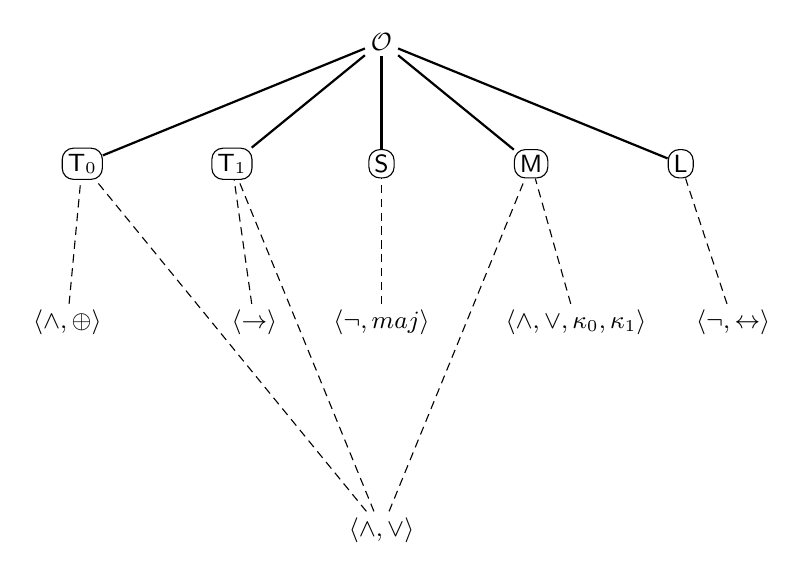
\begin{tikzpicture}[x=1.9cm,y=1.55cm,every node/.style={inner sep=2pt,font=\small}]
 \node (O) at (2,3) {\(\mathcal O\)};
 \node[draw,rounded corners] (t0) at (0,2) {\(\mathsf T_0\)};
 \node[draw,rounded corners] (t1) at (1,2) {\(\mathsf T_1\)};
 \node[draw,rounded corners] (s)  at (2,2) {\(\mathsf S\)};
 \node[draw,rounded corners] (m)  at (3,2) {\(\mathsf M\)};
 \node[draw,rounded corners] (l)  at (4,2) {\(\mathsf L\)};
 \foreach \k in {t0,t1,s,m,l} \draw[thick] (O)--(\k);
 \node (xa) at (-0.1,0.7) {\(\langle\land,\oplus\rangle\)};
 \node (im) at (1.15,0.7) {\(\langle\to\rangle\)};
 \node (nm) at (2,0.7) {\(\langle\neg,\operatorname{maj}\rangle\)};
 \node (mk) at (3.3,0.7) {\(\langle\land,\lor,\kappa_0,\kappa_1\rangle\)};
 \node (ne) at (4.35,0.7) {\(\langle\neg,\leftrightarrow\rangle\)};
 \node (aj) at (2,-1.0) {\(\langle\land,\lor\rangle\)};
 \draw[densely dashed] (xa)--(t0); \draw[densely dashed] (im)--(t1);
 \draw[densely dashed] (nm)--(s);  \draw[densely dashed] (mk)--(m);
 \draw[densely dashed] (ne)--(l);
 \draw[densely dashed] (aj)--(t0); \draw[densely dashed] (aj)--(t1);
 \draw[densely dashed] (aj)--(m);
\end{tikzpicture}
\caption{The top of the lattice of clones of Boolean operations.  Solid
lines: \(\mathcal O\) covers exactly the five boxed maximal clones
(\cref{thm:p02-w02-p02-008-maximal}).  Dashed lines: each lower node, the
clone generated by a basis of \cref{thm:p02-w02-p02-008-bases} (with
\(\kappa_b\) for \(\kappa^1_b\)), is joined to every maximal clone that
includes it, and to no other.  These are inclusions, not necessarily covers;
inclusions among the lower nodes and all other clones of the lattice, which
has infinitely many members, are not drawn.}
\label{fig:p02-w02-p02-008-clones}
\end{figure}

\begin{hbexample}{def:p02-w02-p02-008-worked}{Conjunction from implication and falsum}
Take the connective set \(\{\to,\bottom\}\), so \(C^+=\{\to,\kappa^1_0\}\).
By Table~\ref{tab:p02-w02-p02-008-profile}, \(\to\) lies outside
\(\mathsf T_0\), \(\mathsf S\), \(\mathsf M\) and \(\mathsf L\), and
\(\kappa^1_0\) lies outside \(\mathsf T_1\); the set is complete.  The proof
of \cref{thm:p02-w02-p02-008-criterion} then produces the following
formulas, each checked on its truth table.
\begin{enumerate}
\item \emph{Constants.}  The diagonal of \(\to\) is
  \(x\mapsto(x\to x)\), the constant \(1\), represented by
  \(p_1\to p_1\); the constant \(0\) is represented by \(\bottom\).
\item \emph{Negation.}  The monotonicity test fails for \(\to\) at
  \(\bar a=(0,0)\) and \(i=1\): \((0\to0)=1\) and \((1\to0)=0\).  Fixing
  the second argument at \(0\) gives \(\neg x=x\to0\), represented by
  \(p_1\to\bottom\).
\item \emph{Conjunction.}  The algebraic normal form of \(\to\) is
  \(1\oplus x\oplus xy\), with the single nonlinear monomial \(xy\).  In the
  notation of the proof, \(p(x,y)=xy\oplus x\oplus1\), so the coefficients
  are \(\alpha=1\), \(\beta=0\), \(\gamma=1\), and
  \(xy=p(x,\,1\oplus y)\oplus1\).  That is,
  \(x\land y=\neg(x\to\neg y)\), represented by
  \((p_1\to(p_2\to\bottom))\to\bottom\).  Its truth table is \(1\) only at
  \((1,1)\): there \(p_2\to\bottom\) is \(0\), \(p_1\to0\) is \(0\), and the
  outer implication gives \(1\); at every other row \(p_1\to(p_2\to\bottom)\)
  is \(1\) and the outer implication gives \(0\).
\end{enumerate}
From negation and conjunction, \cref{thm:p02-w02-p02-008-neg-and} supplies
every operation of positive arity, and the closed formulas \(\bottom\) and
\(\bottom\to\bottom\) supply the two nullary constants.
\end{hbexample}

\begin{hbwarning}{def:p02-w02-p02-008-limits}{Scope of the criterion}
\begin{enumerate}
\item The criterion is about expressibility: which truth functions are
  compositions of given ones.  It says nothing about derivability, and a
  complete connective set does not come with a complete calculus.
\item It is a positive-arity result.  Clones contain no nullary function,
  and a connective set without a nullary member is never nullary-inclusive
  functionally complete (\cref{thm:p02-w02-p02-008-nullary}); nullary
  constants of a language enter the criterion only as unary constant
  operations.
\item It is specific to two truth values.  The proof uses that there are
  exactly four unary operations on \(\mathbb B\) and that a
  non-monotone or non-affine operation over \(\mathbb B\) yields negation or
  conjunction; nothing here classifies operations on a set with more than
  two elements.
\item The criterion decides whether every operation is definable; it gives
  no bound on the size of the defining formulas.
\end{enumerate}
\end{hbwarning}

\subsection{Relationships and sources}
\label{sec:p02-w02-p02-008-relationships}

\emph{The basis theorem.}  The functionally complete basis
\(\{\neg,\land,\bottom\}\) of Section~\ref{sec:prop-syntax-semantics-04} is an
instance of \cref{thm:p02-w02-p02-008-criterion}: \(\neg\) lies outside
\(\mathsf T_0\) and \(\mathsf M\), \(\land\) outside \(\mathsf S\) and
\(\mathsf L\), and \(\kappa^1_0\) outside \(\mathsf T_1\); and \(\bottom\) is
a nullary member, so completeness is nullary-inclusive.

\emph{Post's classification.}  Post works with two-valued functions of
variables drawn from a fixed denumerable list, and calls a system of such
functions iteratively closed, or closed, when replacing the arguments of any
of its functions by variables or by functions of the system again gives a
function of the system \cite[\S\,1, pp.~10--11]{Post1941}.  He excludes
functions of no variables, that is, constants, from the classification
\cite[Introduction, pp.~2--3, n.~5]{Post1941}; this is the positive-arity
convention of \cref{def:p02-w02-p02-008-arity}.  In his notation the
complete system is \(C_1\); every closed system properly included in \(C_1\)
is included in at least one of \(C_2\), \(C_3\), \(D_3\), \(A_1\) and
\(L_1\), and none of these five is properly included in another
\cite[\S\,25, pp.~98--99]{Post1941}.  He concludes that a set of generators
yields the complete system exactly when each of the five fails to contain it
\cite[\S\,26, p.~105]{Post1941}.  The five systems are the five classes of
\cref{def:p02-w02-p02-008-five}, as follows.
\begin{itemize}
\item Post describes \(D_3\) as the system of all self-dual functions and
  \(L_1\) as the system of all alternating functions
  \cite[\S\,26, p.~106]{Post1941}.  So \(D_3=\mathsf S\).  A function is
  alternating when replacing any one argument by its negation either leaves
  the function unchanged or turns it into its negation
  \cite[\S\,15, p.~55]{Post1941}, and by
  \cref{thm:p02-w02-p02-008-alternating} below these are exactly the affine
  functions; so \(L_1=\mathsf L\).
\item Post sorts functions by the one-variable function obtained by
  identifying all arguments, calling a function an \(\alpha\)-,
  \(\beta\)-, \(\gamma\)- or \(\delta\)-function according as that function
  is the identity, the constant \(1\), the constant \(0\) or negation
  \cite[\S\,10, p.~43]{Post1941}.  He notes that a set of generators escapes
  \(C_2\) only if it has a \(\gamma\)- or \(\delta\)-function, and escapes
  \(C_3\) only if it has a \(\beta\)- or \(\delta\)-function
  \cite[\S\,26, p.~105]{Post1941}.  The \(\alpha\)- and
  \(\beta\)-functions are exactly the members of \(\mathsf T_1\), so
  \(\mathsf T_1\subseteq C_2\); since \(C_2\) is not the complete system and
  \(\mathsf T_1\) is maximal (\cref{thm:p02-w02-p02-008-maximal}),
  \(C_2=\mathsf T_1\).  In the same way the \(\alpha\)- and
  \(\gamma\)-functions are the members of \(\mathsf T_0\), and
  \(C_3=\mathsf T_0\).
\item Post's \(A_1\) is the system of all functions satisfying his
  \([A{:}a]\) condition \cite[\S\,26, p.~106]{Post1941}.  The clone
  \(\mathsf M\) is closed in Post's sense and is not \(\mathcal O\), so by
  his inclusion result it lies in one of the five systems; it lies in none of
  \(C_2=\mathsf T_1\), \(C_3=\mathsf T_0\), \(D_3=\mathsf S\),
  \(L_1=\mathsf L\), because \(\kappa^1_0\), \(\kappa^1_1\) and \(\land\)
  are monotone and lie outside \(\mathsf T_1\) and \(\mathsf S\),
  \(\mathsf T_0\), and \(\mathsf L\) respectively
  (Table~\ref{tab:p02-w02-p02-008-profile}).  So
  \(\mathsf M\subseteq A_1\), and maximality of \(\mathsf M\) gives
  \(A_1=\mathsf M\).  Consistently, Post records that every
  \(\delta\)-function fails the \([A{:}a]\) condition
  \cite[\S\,26, p.~106]{Post1941}, while a monotone \(f\) has
  \(f(\bar0)\leq f(\bar1)\) and so cannot have negation as its diagonal.
\end{itemize}
The proofs in the annex do not use this comparison; it fixes which of Post's
systems each table row names.

\begin{hblemma}{thm:p02-w02-p02-008-alternating}{proved=annex:p02-w02-p02-008-alt}{Alternating means affine}
For \(f\in\mathcal O_n\), \(f\in\mathsf L\) iff for every \(i\leq n\) either
\(f(\bar a[i{:=}1-a_i])=f(\bar a)\) for every \(\bar a\), or
\(f(\bar a[i{:=}1-a_i])=1-f(\bar a)\) for every \(\bar a\).
\end{hblemma}

\emph{The clone lattice.}  Post's classification is of all closed systems,
not only the maximal ones.  The set of closed systems is infinite
\cite[\S\,25, p.~96]{Post1941}, and Post draws the whole inclusion relation in
an inclusion diagram in which a downward line joins each system to each
system it immediately includes \cite[\S\,25, p.~100]{Post1941}.
Figure~\ref{fig:p02-w02-p02-008-clones} is the top of that two-valued
diagram: its five boxed nodes are Post's \(C_3\), \(C_2\), \(D_3\), \(A_1\)
and \(L_1\), and the lines from \(\mathcal O\) are the five immediate
inclusions under \(C_1\).  The classification concerns operations on the
two-element set \(\mathbb B\) only; nothing in this section concerns
truth functions with more than two values.

\emph{Elsewhere in this part.}  The normal forms of
Section~\ref{sec:prop-syntax-semantics-04} supply, in formula form, the
disjunctive construction behind \cref{thm:p02-w02-p02-008-neg-and}.
\index{Post's criterion}

%% toc: P2 11 11.8
\section{Sheffer stroke, NOR, and proofs of expressive limitations}
\label{sec:p02-w02-p02-009-sheffer}
\index{Sheffer function}\index{functional completeness!single connective}

The note on the sixteen binary truth functions
(Section~\ref{sec:p01-sixteen-functions}) records that NAND and NOR are each
functionally complete, and Section~\ref{sec:p02-w02-p02-008-sheffer} proves
this for positive arities and shows that among the operations of arity at
most two they are the only ones that generate every operation on their own.
This section settles the same question for a single operation of any arity,
and for a single connective together with the nullary constants, in each of
the two scopes of completeness of \cref{def:p02-w02-p02-008-completeness}.
It also proves non-definability results for single operations that pass
some, but not all, of the tests: an operation can reverse both constant
inputs and still be confined to a proper clone.

\emph{Purpose.}  To decide, from three entries of a truth table and one
symmetry check, whether one connective suffices for every truth function,
and to say exactly what changes when the nullary truth functions are
included.

\emph{Inputs.}  From Section~\ref{sec:p02-w02-p02-008-post}: Boolean
operations, composition, clones and generated clones
(\cref{def:p02-w02-p02-008-operations,thm:p02-w02-p02-008-generated}); the
operation set \(C^+\) of a connective set and the positive-arity convention
(\cref{def:p02-w02-p02-008-arity}); positive-arity and nullary-inclusive
completeness (\cref{def:p02-w02-p02-008-completeness}); the five classes
\(\mathsf T_0,\mathsf T_1,\mathsf S,\mathsf M,\mathsf L\) and their tests
(\cref{def:p02-w02-p02-008-five,thm:p02-w02-p02-008-tests}); the fact that
they are clones (\cref{thm:p02-w02-p02-008-five-clones}); Post's criterion
(\cref{thm:p02-w02-p02-008-criterion}); and the NAND and NOR identities
(\cref{thm:p02-w02-p02-008-nand-nor}).  Notation is that of
\cref{def:p02-w02-p02-008-bits}: truth values are \(0,1\), \(\bar0\) and
\(\bar1\) are the constant tuples, and \(\bar a^{\,c}\) is the complement of
\(\bar a\).

\emph{Conclusions.}  Consequences of reversing the constant inputs
(\cref{thm:p02-w02-p02-009-two-tests}); the characterization of single
generators of every arity (\cref{thm:p02-w02-p02-009-sheffer}) and their
number (\cref{thm:p02-w02-p02-009-count}); the completeness of a single
connective, alone and with \(\bottom\) or \(\topv\), in both scopes
(\cref{thm:p02-w02-p02-009-single}); and ternary instances, positive and
negative (\cref{thm:p02-w02-p02-009-ternary}).  Every proof is in the annex.

\subsection{Single generators}
\label{sec:p02-w02-p02-009-single-generators}

\begin{hbdefinition}{def:p02-w02-p02-009-sheffer-op}{Sheffer operation, Sheffer connective}
An operation \(f\in\mathcal O\) is a \emph{Sheffer operation} iff
\(\langle\{f\}\rangle=\mathcal O\), that is, iff every Boolean operation of
positive arity is obtained from \(f\) and the projections by composition.
A truth-functional connective of positive arity is a \emph{Sheffer
connective} iff its interpreting operation is a Sheffer operation.  A
nullary connective is never called a Sheffer connective; its role is settled
separately in \cref{thm:p02-w02-p02-009-single}(1).
\index{Sheffer operation}
\end{hbdefinition}

By \cref{thm:p02-w02-p02-008-formulas-clone}, \(c\) is a Sheffer connective
iff the one-member connective set \(\{c\}\) is positive-arity functionally
complete.  For an \(n\)-ary \(f\), call \(x\mapsto f(x,\ldots,x)\) its
\emph{diagonal}.  The diagonal is negation exactly when \(f(\bar0)=1\) and
\(f(\bar1)=0\), which is the condition \(f\notin\mathsf T_0\) and
\(f\notin\mathsf T_1\).

\begin{hblemma}{thm:p02-w02-p02-009-two-tests}{proved=annex:p02-w02-p02-009-two-tests}{Reversed constants}
Let \(n\geq1\) and \(f\in\mathcal O_n\).
\begin{enumerate}
\item If \(f(\bar0)=1\) and \(f\in\mathsf M\), then \(f=\kappa^n_1\).  If
  \(f(\bar1)=0\) and \(f\in\mathsf M\), then \(f=\kappa^n_0\).
\item If \(f(\bar0)=1\) and \(f(\bar1)=0\), then \(f\notin\mathsf M\).
\item If \(f(\bar0)=1\), \(f(\bar1)=0\) and \(f\in\mathsf L\), then
  \(f\in\mathsf S\).
\end{enumerate}
\end{hblemma}

\begin{hbtheorem}{thm:p02-w02-p02-009-sheffer}{proved=annex:p02-w02-p02-009-sheffer}{Sheffer operations of every arity}
Let \(n\geq1\) and \(f\in\mathcal O_n\).  Then \(f\) is a Sheffer operation
iff
\begin{enumerate}
\item \(f(\bar0)=1\),
\item \(f(\bar1)=0\), and
\item \(f\) is not self-dual: there is \(\bar a\in\mathbb B^n\) with
  \(f(\bar a^{\,c})=f(\bar a)\).
\end{enumerate}
In particular no unary operation is a Sheffer operation, and an operation
whose diagonal is negation is a Sheffer operation iff it is not self-dual.
\end{hbtheorem}

The three conditions are tested on the truth table with at most
\(2+2^{n-1}\) evaluations: the rows \(\bar0\) and \(\bar1\), and the
\(2^{n-1}\) rows with \(a_1=0\) for self-duality
(\cref{thm:p02-w02-p02-008-tests}(1)).  For \(n=2\) the theorem gives back
\cref{thm:p02-w02-p02-008-sheffer}: the binary operations with
\(f(0,0)=1\) and \(f(1,1)=0\) are \(\mathrm{NAND}\), \(\mathrm{NOR}\),
\((x,y)\mapsto1-x\) and \((x,y)\mapsto1-y\), and the last two are self-dual.

\begin{hbcorollary}{thm:p02-w02-p02-009-count}{proved=annex:p02-w02-p02-009-count}{Number of Sheffer operations}
For \(n\geq1\), the number of Sheffer operations in \(\mathcal O_n\) is
\[
  2^{2^n-2}-2^{2^{n-1}-1}.
\]
It is \(0\) for \(n=1\), \(2\) for \(n=2\), \(56\) for \(n=3\) and
\(16256\) for \(n=4\).  The proportion of Sheffer operations among the
\(2^{2^n}\) members of \(\mathcal O_n\) is
\(\tfrac14-2^{-2^{n-1}-1}\), which increases with \(n\) and tends to
\(\tfrac14\).
\end{hbcorollary}

\subsection{One connective and the nullary constants}
\label{sec:p02-w02-p02-009-scope}

The definition of functional completeness in
Section~\ref{sec:prop-syntax-semantics-04} quantifies over every arity, \(0\)
included (\cref{def:p02-w02-p02-008-completeness}).  The next theorem keeps
the two scopes apart for every connective set with one member, and for one
connective of positive arity together with \(\bottom\) (value \(0\)), with a
nullary verum \(\topv\) (value \(1\)), or with both.

\begin{hbtheorem}{thm:p02-w02-p02-009-single}{proved=annex:p02-w02-p02-009-single}{Single connectives in both scopes}
\begin{enumerate}
\item If \(c\) is a nullary connective, \(\{c\}\) is neither positive-arity
  nor nullary-inclusive functionally complete.
\item Let \(c\) be a connective of arity \(n\geq1\) interpreted by
  \(f\in\mathcal O_n\).  Then \(\{c\}\) is positive-arity functionally
  complete iff \(f\) satisfies the three conditions of
  \cref{thm:p02-w02-p02-009-sheffer}; and \(\{c\}\) is never
  nullary-inclusive functionally complete.
\item Consequently no connective set with exactly one member is
  functionally complete in the sense of
  Section~\ref{sec:prop-syntax-semantics-04}.
\item Let \(c\) and \(f\) be as in part~2.  Each of the following sets has a
  nullary member, so for each of them positive-arity and nullary-inclusive
  functional completeness coincide, and:
  \begin{enumerate}
  \item \(\{c,\bottom\}\) is functionally complete iff \(f(\bar0)=1\) and
    \(f\notin\mathsf L\);
  \item \(\{c,\topv\}\) is functionally complete iff \(f(\bar1)=0\) and
    \(f\notin\mathsf L\);
  \item \(\{c,\bottom,\topv\}\) is functionally complete iff
    \(f\notin\mathsf M\) and \(f\notin\mathsf L\).
  \end{enumerate}
  In case~(a) the closed formula \(c(\bottom,\ldots,\bottom)\) represents
  the constant \(1\); in case~(b) the closed formula
  \(c(\topv,\ldots,\topv)\) represents the constant \(0\).
\item If \(c\) is a Sheffer connective, all three sets of part~4 are
  functionally complete.
\end{enumerate}
\end{hbtheorem}

For \(\mathrm{NAND}\) and \(\mathrm{NOR}\), part~2 restates
\cref{thm:p02-w02-p02-008-nand-nor}(2)--(3): each is positive-arity complete
and neither alone represents a nullary truth function.  Part~4 shows that
adding a constant does not require a Sheffer connective: \(\{\to,\bottom\}\)
is complete because \((0\to0)=1\) and \(\to\) is not affine, while
\(\{\to,\topv\}\) is not, because \((1\to1)=1\), so that every operation
generated lies in \(\mathsf T_1\).

\subsection{Ternary instances and limitations}
\label{sec:p02-w02-p02-009-ternary}

A non-definability claim is proved by exhibiting a clone that contains the
given operations but not the target: by
\cref{thm:p02-w02-p02-008-generated}(5) the generated clone stays inside it,
and by \cref{thm:p02-w02-p02-008-formulas-clone} so does the truth function of
every formula over the connective set.  In the next theorem the operations
are given by their values on \(\bar a=(x,y,z)\in\mathbb B^3\);
\(\operatorname{maj}\) is the majority operation of
Section~\ref{sec:p02-w02-p02-008-clones}.

\begin{hbtheorem}{thm:p02-w02-p02-009-ternary}{proved=annex:p02-w02-p02-009-ternary}{Ternary instances}
\begin{enumerate}
\item The ternary operations \(1\oplus xyz\) and
  \((1\oplus x)(1\oplus y)(1\oplus z)\), the three-place NAND and NOR, are
  Sheffer operations.  Identifying the last two arguments of each gives
  \(\mathrm{NAND}\), respectively \(\mathrm{NOR}\).
\item The operation \(g(x,y,z)=1\oplus\operatorname{maj}(x,y,z)\) satisfies
  \(g(\bar0)=1\) and \(g(\bar1)=0\), and lies in \(\mathsf S\) and in none of
  \(\mathsf T_0,\mathsf T_1,\mathsf M,\mathsf L\).  Hence
  \(\langle\{g\}\rangle\subseteq\mathsf S\): no formula over a connective
  set whose operation set is \(\{g\}\) represents \(\land\), \(\lor\), \(\to\),
  \(\mathrm{NAND}\), \(\mathrm{NOR}\) or a constant operation.
\item The operation \(h(x,y,z)=1\oplus x\oplus y\oplus z\) satisfies
  \(h(\bar0)=1\) and \(h(\bar1)=0\), and lies in \(\mathsf S\) and
  \(\mathsf L\) and in none of \(\mathsf T_0,\mathsf T_1,\mathsf M\).  Hence
  \(\langle\{h\}\rangle\subseteq\mathsf S\cap\mathsf L\): besides the
  operations excluded in part~2, it excludes \(\operatorname{maj}\), which
  is not affine.
\item The operation \(f(x,y,z)=(1-x)\cdot(y\to z)\) is a Sheffer
  operation, and for all \(x,y,z\in\mathbb B\):
  \(f(x,x,x)=1-x\), \(f(x,1-x,x)=0\) and \(f(0,y,z)=(y\to z)\).
\end{enumerate}
\end{hbtheorem}

\begin{hbexample}{def:p02-w02-p02-009-worked}{A ternary Sheffer connective and its definitions}
Let \(c\) be a ternary connective interpreted by
\(f(x,y,z)=(1-x)\cdot(y\to z)\), that is, by \(\neg x\land(y\to z)\).  Its
truth table has the value \(1\) exactly at \((0,0,0)\), \((0,0,1)\) and
\((0,1,1)\).
\begin{enumerate}
\item \emph{Tests.}  \(f(0,0,0)=1\) and \(f(1,1,1)=0\).  At
  \(\bar a=(0,1,0)\), \(f(\bar a)=1\cdot(1\to0)=0\) and
  \(f(\bar a^{\,c})=f(1,0,1)=0\); so \(f\) is not self-dual, and
  \cref{thm:p02-w02-p02-009-sheffer} makes \(c\) a Sheffer connective.
\item \emph{Negation.}  The diagonal is
  \(f(x,x,x)=(1-x)\cdot(x\to x)=1-x\); so \(c(p_1,p_1,p_1)\) represents
  \(\neg p_1\).
\item \emph{A constant.}  The witness \((0,1,0)\) of non-self-duality gives
  \(k(x)=f(x,1-x,x)\), with \(k(0)=f(0,1,0)=0\) and \(k(1)=f(1,0,1)=0\); so
  \(k=\kappa^1_0\), represented by
  \(\theta\defeq c(p_1,c(p_1,p_1,p_1),p_1)\).
\item \emph{Implication.}  \(f(0,y,z)=y\to z\), so
  \(f(k(x),x,y)=(x\to y)\) for all \(x,y\); the formula
  \(\iota\defeq c(\theta,p_1,p_2)\) represents \(p_1\to p_2\).
\item \emph{Conjunction.}  \(x\land y=\neg(x\to\neg y)\), so
  \(p_1\land p_2\) is represented by
  \(c(\iota',\iota',\iota')\) with \(\iota'\) the result of replacing \(p_2\)
  by \(c(p_2,p_2,p_2)\) in \(\iota\).
\end{enumerate}
The identities used in items~2 to~4 are part~4 of
\cref{thm:p02-w02-p02-009-ternary}; its proof also checks the five formulas
on every row.  From
\(\neg\) and \(\land\) every operation of positive arity follows
(\cref{thm:p02-w02-p02-008-neg-and}).  The connective set \(\{c\}\) still
has no closed formula; \(\{c,\bottom\}\) obtains the constant \(1\) as
\(c(\bottom,\bottom,\bottom)\), by \cref{thm:p02-w02-p02-009-single}(4).
\end{hbexample}

\begin{hbwarning}{def:p02-w02-p02-009-limits}{What a single connective does not give}
\begin{enumerate}
\item Reversing both constant rows is necessary and not sufficient: \(g\)
  and \(h\) of \cref{thm:p02-w02-p02-009-ternary} reverse them and are
  confined to \(\mathsf S\).  The self-duality test cannot be omitted.
\item ``NAND alone is functionally complete'' holds in the positive-arity
  scope only.  By \cref{thm:p02-w02-p02-009-single}(3), no one-member
  connective set is complete in the scope of
  Section~\ref{sec:prop-syntax-semantics-04}, which includes the two
  nullary truth functions; a Sheffer connective needs \(\bottom\) or
  \(\topv\) beside it.
\item A Sheffer connective defines every truth function, and the
  definitions can be long: the representation of \(\land\) in
  \cref{def:p02-w02-p02-009-worked} has three copies of \(\iota'\).  The
  results here give no bound on formula size.
\item The characterization concerns operations on the two-element set
  \(\mathbb B\); the lemma behind it uses that the only truth values are
  \(0\) and \(1\), and nothing here applies to more than two truth values.
\end{enumerate}
\end{hbwarning}

\subsection{Relationships and sources}
\label{sec:p02-w02-p02-009-relationships}

\emph{Within this part.}  The single-generator theorem is the one-member case
of Post's criterion (\cref{thm:p02-w02-p02-008-criterion}), with
\cref{thm:p02-w02-p02-009-two-tests} removing the monotone and affine tests.
The binary case is \cref{thm:p02-w02-p02-008-sheffer}; the explicit NAND and
NOR definitions of negation, conjunction and the constants are in
\cref{thm:p02-w02-p02-008-nand-nor}; the general negative and positive bases
are in \cref{thm:p02-w02-p02-008-bases}.  The note on the sixteen binary
functions in Section~\ref{sec:p01-sixteen-functions} states NAND and NOR
completeness without the scope; \cref{thm:p02-w02-p02-009-single}(2)--(3)
supply it.

\emph{Post's terms.}  Post calls a function an \(\alpha\)-, \(\beta\)-,
\(\gamma\)- or \(\delta\)-function according as the one-variable function
obtained by putting one variable for all arguments is the identity, the
constant \(1\), the constant \(0\) or negation \cite[\S\,10,
p.~43]{Post1941}.  So the conditions \(f(\bar0)=1\), \(f(\bar1)=0\) of
\cref{thm:p02-w02-p02-009-sheffer} say that \(f\) is a
\(\delta\)-function.  Post's list of all sets of independent generators of
the complete system begins with the form consisting of a single
non-self-dual \(\delta\)-function \cite[\S\,26, p.~107]{Post1941}.  He
obtains it from the remark that an alternating \(\delta\)-function is
self-dual, so that a sole generator need only be a non-self-dual
\(\delta\)-function \cite[\S\,26, p.~108]{Post1941}; in the present terms
that remark is \cref{thm:p02-w02-p02-009-two-tests}(3), alternating
functions being the affine ones (\cref{thm:p02-w02-p02-008-alternating}).
Post reports that Sheffer introduced the binary functions he calls
rejection and incompatibility, that is, NOR and NAND, and that Nicod used the
latter \cite[\S\,26, p.~117]{Post1941}; and that an earlier study by
Zylinski determined which binary functions are generated by single binary
functions \cite[Introduction, p.~6]{Post1941}.  The count of
\cref{thm:p02-w02-p02-009-count} and the statements about constants in
\cref{thm:p02-w02-p02-009-single} are proved here and are not taken from
Post, who excludes constants from his systems
\cite[Introduction, p.~2, n.~5]{Post1941}.
\index{Post's criterion!single generator}

%% toc: P2 15 15.1,15.2,15.3,15.8
\section{Decision bounds, reductions and checked certificates for propositional satisfiability}
\label{sec:p02-w02-p02-018-decision-certificates}

\emph{Purpose.}  The propositional resolution rule, its soundness and its
refutation completeness are the exact inherited results of
\cref{sec:prop-metatheory-04}, with the refutation displayed as a graph in
Figure~\ref{fig:p02-resolution-dag}.  This section supplies what those results
do not: an explicit input representation for the four finite decision problems
of classical propositional logic, a truth-table procedure for them with a
written termination, correctness and running-time proof, the exact limits of
that decidability claim, the proofs that \(\mathsf{SAT}\) is in
\(\mathsf{NP}\), that \(\mathsf{TAUT}\) is in \(\mathsf{coNP}\), that negation
interreduces \(\mathsf{SAT}\) with the complement of \(\mathsf{TAUT}\), and
that every \(\mathsf{NP}\) problem reduces to \(\mathsf{SAT}\), and finally
three checked certificate formats with a worked instance of each, together
with a fully annotated first-order resolution refutation.

\emph{Inputs.}  Finite strings over the fixed token alphabet of
\cref{def:p02-w02-p02-018-input}, presenting a formula, a finite list of
premises with a conclusion, or a pair of formulas; and, for the certificate
checks, finite clause sets with a candidate valuation or a candidate
refutation log.  \emph{Conclusions.}  A yes or no answer with a witness
valuation where one exists, a bound on the number of machine steps, and
checked evidence for satisfiability, unsatisfiability and failure of
consequence.

\emph{Standing notation.}  Formulas are the members of
\(\mathsf{Fm}_{\mathsf{CPL}}\) of \cref{sec:prop-syntax-semantics-01}, with
primitive \(\bottom,\neg,\land,\lor,\to\) and variables \(p_n\)
(\(n\in\N\)).  A valuation \(v\) assigns \(\mathbf T\) or \(\mathbf F\) to
every variable, \(\widehat v\) is its extension to formulas, and
satisfaction, satisfiability, validity, semantic consequence
\(\Gamma\entails\varphi\) and logical equivalence are those of
\cref{sec:prop-syntax-semantics-02}.  \(\operatorname{Var}(e)\) is the finite
set of variables occurring in \(e\).  Clauses, the clause interpretation
\(\operatorname{form}_{\mathsf{CPL}}\) and literal complements
\(\overline L\) are those of \cref{sec:prop-syntax-semantics-04,%
sec:prop-metatheory-04}.  In examples \(p,q,r\) are the distinct variables
\(p_0,p_1,p_2\).  The complexity classes, reductions and the languages
\(\mathsf{SAT}\) and \(\mathsf{TAUT}\) are those of
\cref{def:p02-complexity-standing,def:p02-sat-taut}.

\subsection{The declared input representation}
\label{sec:p02-w02-p02-018-input}

\begin{hbconvention}{def:p02-w02-p02-018-input}{Effective finite inputs for classical propositional logic}
\emph{Tokens.}  The token alphabet consists of the thirteen distinct symbols
\[
 \texttt{p},\ \texttt{0},\ \texttt{1},\ \texttt{;},\ \bottom,\ \neg,\
 \land,\ \lor,\ \to,\ (,\ ),\ \texttt{,}\ ,\ \texttt{|}\ ,
\]
listed here in a fixed order; the token in position \(i\) of this list
(\(0\leq i\leq 12\)) is encoded by the four-bit binary numeral of \(i\).
Every input is a bit string; it is \emph{decodable} when its length is a
multiple of \(4\) and each consecutive group of four bits is the code of a token.
Write \(m\) for the bit length of an input, so a decodable input has \(m/4\)
tokens.

\emph{Formulas.}  The variable \(p_n\) is written as the token \texttt{p},
followed by the binary numeral of \(n\) without leading zeros (the single
digit \texttt{0} when \(n=0\)), followed by the terminator \texttt{;}.  A
formula is written as its fully parenthesized string of
\cref{sec:prop-syntax-semantics-01} with each variable so written; the
separators \texttt{,} and \texttt{|} do not occur in formula strings.  This
is the formula encoding of \cref{def:p02-sat-taut} with its code table
fixed.

\emph{Instances.}  The four decision problems are the following sets of bit
strings.
\begin{enumerate}
\item \(\mathsf{SAT}\): encodings of satisfiable formulas.
\item \(\mathsf{TAUT}\): encodings of valid formulas.
\item \(\mathsf{CONS}\): encodings of strings
      \(\gamma_1\,\texttt{,}\,\gamma_2\,\texttt{,}\cdots\texttt{,}\,\gamma_r\,
      \texttt{|}\,\varphi\) with \(r\geq0\) formula strings before the
      separator \texttt{|} (for \(r=0\) the string begins with \texttt{|})
      such that \(\{\gamma_1,\ldots,\gamma_r\}\entails\varphi\).  The list
      presents the finite premise set \(\Gamma=\{\gamma_1,\ldots,\gamma_r\}\);
      order and repetition in the list do not affect membership.
\item \(\mathsf{EQV}\): encodings of strings
      \(\varphi\,\texttt{|}\,\psi\) of two formula strings such that
      \(\varphi\) and \(\psi\) are logically equivalent.
\end{enumerate}
A bit string that is not decodable, or whose token string does not have the
displayed shape with formula strings in the displayed positions, is
\emph{malformed} and belongs to none of the four sets.  For an instance
\(x\), \(k\) denotes the number of distinct variables occurring in it.
Because every variable occurrence uses at least three tokens,
\(k\leq m/12\).

The names \(\mathsf{CONS}\) and \(\mathsf{EQV}\) are needed to state the
consequence and equivalence problems as sets of strings beside the two
languages of \cref{def:p02-sat-taut}; they are metalinguistic names of
languages, not connectives, and are used in
\cref{thm:p02-w02-p02-018-decision}.  Any other representation reaches these
results only through a computable translation into this one.
\index{CONS@\(\mathsf{CONS}\)}\index{EQV@\(\mathsf{EQV}\)}
\index{input representation!propositional decision problems}
\end{hbconvention}

\subsection{The truth-table decision procedure and its bound}
\label{sec:p02-w02-p02-018-truth-table}

\begin{hbmethod}{def:p02-w02-p02-018-evaluator}{Stack evaluation of formula strings}
\emph{Input.}  A token string \(w\) without separators, and a
\emph{valuation table} \(\tau\): a finite list of pairs \((n,b)\), each a
binary numeral \(n\) and a truth value \(b\), with no numeral listed twice.
The table determines the valuation \(v_\tau\) that gives \(p_n\) the value
\(b\) when \((n,b)\) is listed and \(\mathbf F\) otherwise.

\emph{Procedure.}  Start with an empty stack whose entries are truth values
or the markers \(\neg\), \((\), \(\land\), \(\lor\), \(\to\).  To
\emph{reduce} the stack, repeat: while the top entry is a truth value \(b\)
and the entry below it is \(\neg\), replace these two entries by the
opposite value of \(b\).  Read \(w\) from left to right.
\begin{enumerate}
\item On \texttt{p}: read the following digit tokens up to the next
      \texttt{;}.  If no \texttt{;} follows, if the digit string is empty, or
      if it has a leading \texttt{0} and more than one digit, stop with the
      answer \emph{malformed}.  Otherwise push the value that \(v_\tau\)
      gives to the variable with this numeral, then reduce.
\item On \(\bottom\): push \(\mathbf F\), then reduce.
\item On \(\neg\), \((\), \(\land\), \(\lor\) or \(\to\): push it.
\item On \()\): if the four top entries are, from the top, a truth value
      \(b\), a binary connective \(\circ\), a truth value \(a\) and \((\),
      replace them by the value of \(a\circ b\) under the truth clause of
      \(\circ\), then reduce; otherwise stop with \emph{malformed}.
\item On any other token stop with \emph{malformed}.
\end{enumerate}
At the end of \(w\), answer \emph{well formed with value \(b\)} if the stack
consists of exactly one truth value \(b\), and \emph{malformed} otherwise.
\end{hbmethod}

\begin{hblemma}{thm:p02-w02-p02-018-evaluator}{proved=annex:p02-w02-p02-018-evaluator}{Correctness and cost of stack evaluation}
Let \(w\) be a token string without separators and \(\tau\) a valuation
table.
\begin{enumerate}
\item Method~\ref{def:p02-w02-p02-018-evaluator} answers \emph{well formed}
      on \(w\) if and only if \(w\) is the string of a formula \(\chi\), and
      then its value is \(\widehat{v_\tau}(\chi)\).
\item On a deterministic machine with a read-only input tape holding \(w\)
      and work tapes holding \(\tau\) and the stack, the method halts within
      \(c\,t\,(t+s)\) steps, where \(t\) is the number of tokens of \(w\),
      \(s\) the number of symbols of the written table and \(c\) a constant
      independent of \(w\) and \(\tau\).
\end{enumerate}
\end{hblemma}

\begin{hbmethod}{def:p02-w02-p02-018-truth-table}{Truth-table decision procedure}
\emph{Input.}  A bit string \(x\) and one of the four problems of
\cref{def:p02-w02-p02-018-input}.

\emph{Step 1 (recognition).}  Decode \(x\) into tokens; split the token string
at its separators; check that the separators have the shape required by the
problem; and run Method~\ref{def:p02-w02-p02-018-evaluator} with the empty
table on each segment.  If any check fails, \emph{reject}.

\emph{Step 2 (variables).}  List the distinct variables of the instance as
\(x_1,\ldots,x_k\) in order of first occurrence, and write the table
\(\tau=((x_1,\mathbf F),\ldots,(x_k,\mathbf F))\).

\emph{Step 3 (rows).}  Visit the \(2^k\) assignments
\(u:\{x_1,\ldots,x_k\}\to\{\mathbf T,\mathbf F\}\) in lexicographic order of
\((u(x_1),\ldots,u(x_k))\) with \(\mathbf F\) before \(\mathbf T\); the table
holds the current row, and the next row is obtained by changing the final
run of \(\mathbf T\) entries to \(\mathbf F\) and the entry before that
run from \(\mathbf F\) to \(\mathbf T\).  For each row evaluate every segment
under \(v_\tau\) by Method~\ref{def:p02-w02-p02-018-evaluator} and stop at the
first row on which
\begin{itemize}
\item for \(\mathsf{SAT}\), the formula is true: \emph{accept} and output the
      row;
\item for \(\mathsf{TAUT}\), the formula is false: \emph{reject} and output
      the row;
\item for \(\mathsf{CONS}\), every premise is true and the conclusion is
      false: \emph{reject} and output the row;
\item for \(\mathsf{EQV}\), the two formulas receive different values:
      \emph{reject} and output the row.
\end{itemize}
\emph{Step 4 (exhaustion).}  If no row stops the search, \emph{reject} for
\(\mathsf{SAT}\) and \emph{accept} for \(\mathsf{TAUT}\), \(\mathsf{CONS}\)
and \(\mathsf{EQV}\).
\index{truth-table decision procedure}
\end{hbmethod}

\begin{hbtheorem}{thm:p02-w02-p02-018-decision}{proved=annex:p02-w02-p02-018-decision}{Decidability with a running-time bound}
For each of \(\mathsf{SAT}\), \(\mathsf{TAUT}\), \(\mathsf{CONS}\) and
\(\mathsf{EQV}\), Method~\ref{def:p02-w02-p02-018-truth-table} halts on every
bit string \(x\) and accepts \(x\) exactly when \(x\) belongs to the problem.
A row output on acceptance for \(\mathsf{SAT}\), extended by \(\mathbf F\) on
all other variables, satisfies the formula; a row output on rejection for
\(\mathsf{TAUT}\), \(\mathsf{CONS}\) or \(\mathsf{EQV}\), so extended,
falsifies the formula, is a countervaluation to
\(\Gamma\entails\varphi\), or separates the two formulas.  On a deterministic
multitape machine the procedure halts within
\[
 c\,(2^{k}+1)\,m^{2}
\]
steps, where \(m\) is the bit length of \(x\), \(k\) the number of distinct
variables of the instance (\(k=0\) for a malformed input) and \(c\) a
constant independent of \(x\).  Every valid formula with \(k\) variables
makes the procedure visit all \(2^{k}\) rows.
\end{hbtheorem}

The bound has two factors: the number of rows, \(2^{k}\), and the cost of one
row, which is at most quadratic in the input length.  The last sentence of
the theorem shows that this procedure attains the exponential factor.  That
is not a lower bound for the problem: a proof that no polynomial-time
procedure decides \(\mathsf{SAT}\) would settle \(\mathsf P\ne\mathsf{NP}\),
since \(\mathsf{SAT}\) is \(\mathsf{NP}\)-complete
(\cref{thm:p02-w02-p02-018-cook-levin}).  The theorem also gives a written
proof of the content of the cited \cref{thm:p02-decidability} for the
representation of \cref{def:p02-w02-p02-018-input}.

\begin{hbwarning}{def:p02-w02-p02-018-scope}{Limits of the decidability theorem}
\Cref{thm:p02-w02-p02-018-decision} decides consequence from a
\emph{finite} premise list presented by the declared encoding, over the
countable variable set \(\{p_n:n\in\N\}\).  It gives no procedure for a fixed
infinite theory \(\Gamma\), and none exists in general: by
\cref{thm:p02-w02-p02-018-limits}(1) there are sets
\(\Gamma\subseteq\{p_n:n\in\N\}\) whose consequence sets are not decided by
any machine.  Compactness (\cref{thm:prop-compactness}) implies that a
consequence of an infinite \(\Gamma\) is already a consequence of a finite
subset, but it does not say how to find that subset from \(\Gamma\).  Nor does the theorem apply to the
languages \(\operatorname{Form}(P)\) of
\cref{def:p02-arbitrary-prop-language} over an arbitrary set \(P\): a
decision procedure acts on finite strings, and by
\cref{thm:p02-w02-p02-018-limits}(2) an uncountable \(P\) has no injective
representation by finite strings at all.  A countable \(P\) is covered only
when it is presented by a computable translation into the declared
encoding.
\end{hbwarning}

\begin{hbtheorem}{thm:p02-w02-p02-018-limits}{proved=annex:p02-w02-p02-018-limits}{Infinite theories and uncountable alphabets}
\begin{enumerate}
\item For \(A\subseteq\N\) let \(\Gamma_A=\{p_n:n\in A\}\).  Then
      \(\Gamma_A\entails p_n\) if and only if \(n\in A\).  Consequently
      the map \(A\mapsto\{\varphi:\Gamma_A\entails\varphi\}\) is injective,
      and for all but countably many \(A\subseteq\N\) the set of encodings
      of formulas \(\varphi\) with \(\Gamma_A\entails\varphi\) is decided by no
      deterministic multitape machine.
\item If \(P\) is uncountable, there is no injective map from \(P\) into the
      set \(\{0,1\}^*\) of finite bit strings.
\end{enumerate}
\end{hbtheorem}

\subsection{Membership, the negation reduction and \texorpdfstring{\(\mathsf{NP}\)}{NP}-hardness}
\label{sec:p02-w02-p02-018-complexity}

\begin{hbconvention}{def:p02-w02-p02-018-verifier}{Verifiers and pairing}
For bit strings \(x=x_1\cdots x_n\) and \(y\), put
\(\langle x,y\rangle\defeq x_1x_1x_2x_2\cdots x_nx_n\,01\,y\).  Reading
the string in consecutive pairs of bits from the left, the first pair
\(01\) separates the two parts, because every earlier pair is \(00\) or
\(11\); so the pairing is injective and both parts are recovered in one
scan.  A predicate
\(R\) of two strings is \emph{polynomial time} when a deterministic multitape
machine decides \(\{\langle x,y\rangle:R(x,y)\}\) in a number of steps bounded
by a polynomial in the length of \(\langle x,y\rangle\).  This fixes the
predicate clause of \cref{def:p02-complexity-standing}.  For
\(L\subseteq\{0,1\}^*\), \(L^{\mathsf c}\) is its complement
\(\{0,1\}^*\setminus L\); thus \(\mathsf{TAUT}^{\mathsf c}\) consists of the
malformed strings and the encodings of formulas that are not valid.
\end{hbconvention}

\begin{hbtheorem}{thm:p02-w02-p02-018-membership}{proved=annex:p02-w02-p02-018-membership}{\(\mathsf{SAT}\) is in \(\mathsf{NP}\) and \(\mathsf{TAUT}\) is in \(\mathsf{coNP}\)}
\(\mathsf{SAT}\in\mathsf{NP}\), witnessed by the certificate that lists the
values of a satisfying valuation on the variables of the formula in order of
first occurrence, checked by one evaluation.  \(\mathsf{TAUT}^{\mathsf c}\in
\mathsf{NP}\), witnessed by a falsifying valuation listed in the same way (or
the empty string for a malformed input); hence \(\mathsf{TAUT}\in
\mathsf{coNP}\).  In both cases the certificate has length at most \(m\) and
the check takes at most \(c\,m^{2}\) steps.
\end{hbtheorem}

\begin{hbtheorem}{thm:p02-w02-p02-018-negation}{proved=annex:p02-w02-p02-018-negation}{The negation reduction}
Let \(h(x)\) be the encoding of \(\neg\varphi\) when \(x\) encodes the formula
\(\varphi\), and the encoding of \(\neg\bottom\) when \(x\) is malformed.
Then \(h\) is computable within \(c\,(m+1)^{2}\) steps on inputs of bit
length \(m\), for a constant \(c\), and, for every bit string \(x\),
\[
 x\in\mathsf{SAT}\iff h(x)\in\mathsf{TAUT}^{\mathsf c},
 \qquad
 x\in\mathsf{TAUT}^{\mathsf c}\iff h(x)\in\mathsf{SAT}.
\]
Consequently, for every \(L\subseteq\{0,1\}^*\), \(L\) has a polynomial-time
many-one reduction to \(\mathsf{SAT}\) if and only if \(L^{\mathsf c}\) has one
to \(\mathsf{TAUT}\).
\end{hbtheorem}

\begin{hbtheorem}{thm:p02-w02-p02-018-cook-levin}{proved=annex:p02-w02-p02-018-cook-levin}{Every \(\mathsf{NP}\) problem reduces to \(\mathsf{SAT}\)}
For every \(L\in\mathsf{NP}\) there is a polynomial-time computable map
\(x\mapsto\varphi_x\), with \(\varphi_x\) an encoded formula, such that
\(x\in L\) iff \(\varphi_x\) is satisfiable.  With
\cref{thm:p02-w02-p02-018-membership}, \(\mathsf{SAT}\) is
\(\mathsf{NP}\)-complete under polynomial-time many-one reductions.
\end{hbtheorem}

\begin{hbcorollary}{thm:p02-w02-p02-018-taut-conp}{proved=annex:p02-w02-p02-018-taut-conp}{\(\mathsf{TAUT}\) is \(\mathsf{coNP}\)-complete}
\(\mathsf{TAUT}\) is \(\mathsf{coNP}\)-complete under polynomial-time
many-one reductions.
\end{hbcorollary}

The formula \(\varphi_x\) describes a run of a polynomial-time verifier for
\(L\) on the input \(x\) and an unknown certificate, step by step, in
variables that record the machine state, the head positions and the cell
contents at each time.  This tableau-of-computation method is the
construction of \textcite[p.~152, Theorem~1]{Cook1971}, which encodes a
one-tape nondeterministic machine and states the result for tautologies in
disjunctive normal form under polynomial-time oracle reducibility.  The
annex encodes a deterministic multitape verifier instead, so that the
reduction is many-one and uses the machine model of
\cref{def:p02-complexity-standing} without a tape-reduction step.  The
reconstruction in \cref{sec:p09-presentation-n-c-026} encodes a one-tape
verifier by windows of three adjacent cells and so presupposes a one-tape
simulation of the verifier; the encoding here follows every head of the
multitape verifier with its own position variables instead.
\Cref{thm:p02-w02-p02-018-cook-levin,thm:p02-w02-p02-018-taut-conp} prove the
statements cited as \cref{thm:p02-sat-np-complete,thm:p02-taut-conp-complete}
and \cref{thm:p04-cook-levin}.  They classify the problems; they do not decide
whether \(\mathsf P=\mathsf{NP}\) or \(\mathsf{NP}=\mathsf{coNP}\).

\subsection{Checked certificates}
\label{sec:p02-w02-p02-018-certificates}

\begin{hbdefinition}{def:p02-w02-p02-018-formats}{Three certificate formats and their checks}
Let \(F\) and \(S\) be finite clause sets, \(\Gamma\) a finite formula set and
\(\varphi\) a formula.
\begin{enumerate}
\item A \emph{satisfying-valuation certificate} for \(F\) is a total
      assignment of truth values to \(\operatorname{Var}(F)\).  Its
      \emph{clause check} visits each clause \(C\in F\) and looks for a literal
      of \(C\) made true by the assignment; it accepts when every clause has
      one.  This is the SAT certificate of
      \cref{def:p12-sat-certificate-boundary}.
\item A \emph{resolution refutation log} for \(S\) is a finite list of
      numbered lines \(1,\ldots,N\).  Line \(i\) carries a clause \(C_i\)
      and a justification, which is either \emph{input} or a triple
      \((j,k,L)\) with \(j,k<i\): the parents \(C_j\), \(C_k\) and the
      pivot literal \(L\).  The \emph{line check} accepts an input line when
      \(C_i\in S\), and a triple line when \(L\in C_j\),
      \(\overline L\in C_k\) and
      \(C_i=(C_j\setminus\{L\})\cup(C_k\setminus\{\overline L\})\).  The
      \emph{log check} accepts when every line passes and \(C_N=\varnothing\).
\item A \emph{countervaluation certificate} for \(\Gamma\entails\varphi\) is
      a total assignment of truth values to
      \(\operatorname{Var}(\Gamma\cup\{\varphi\})\).  Its check evaluates every
      member of \(\Gamma\) and \(\varphi\) under the assignment, extended by
      \(\mathbf F\) elsewhere, and accepts when every member of \(\Gamma\) is
      true and \(\varphi\) is false.
\end{enumerate}
These are finite evidence objects with mechanical checks, distinct from the
semantic facts they establish; the distinction is used in
\cref{thm:p02-w02-p02-018-checks}.
\index{certificate!satisfying valuation}\index{resolution refutation log}
\index{certificate!countervaluation}
\end{hbdefinition}

\begin{hbtheorem}{thm:p02-w02-p02-018-checks}{proved=annex:p02-w02-p02-018-checks}{Soundness and completeness of the three checks}
\begin{enumerate}
\item The clause check accepts an assignment for \(F\) if and only if every
      valuation extending it satisfies \(F\).  So \(F\) is satisfiable iff
      some certificate is accepted.
\item If the log check accepts a log for \(S\), then \(S\) is not
      satisfiable.  If \(S\) is not satisfiable, some log for \(S\) is
      accepted.
\item The countervaluation check accepts an assignment if and only if every
      valuation extending it satisfies \(\Gamma\) and falsifies \(\varphi\).
      So \(\Gamma\not\entails\varphi\) iff some certificate is accepted.
\end{enumerate}
\end{hbtheorem}

\begin{hblemma}{thm:p02-w02-p02-018-extraction}{proved=annex:p02-w02-p02-018-extraction}{Countervaluations from failed searches}
Let \(\Gamma\) be finite.
\begin{enumerate}
\item If Method~\ref{def:p02-w02-p02-018-truth-table} rejects an instance of
      \(\mathsf{CONS}\) presenting \(\Gamma\) and \(\varphi\), its output row,
      restricted to \(\operatorname{Var}(\Gamma\cup\{\varphi\})\), is accepted
      by the countervaluation check.
\item Let \(F_\Gamma\) and \(F_\neg\) be finite clause sets such that every
      valuation satisfying \(F_\Gamma\) satisfies \(\Gamma\), every valuation
      satisfying \(F_\neg\) falsifies \(\varphi\), and
      \(\operatorname{Var}(\Gamma\cup\{\varphi\})\subseteq
      \operatorname{Var}(F_\Gamma\cup F_\neg)\).  If
      Method~\ref{def:p12-dpll} returns a valuation on
      \(F_\Gamma\cup F_\neg\), its restriction to
      \(\operatorname{Var}(\Gamma\cup\{\varphi\})\) is accepted by the
      countervaluation check.
\end{enumerate}
\end{hblemma}

The hypotheses of the second clause hold when each member of \(\Gamma\) and
the formula \(\neg\varphi\) is the conjunctive normal form, in the same
variables, of the corresponding clause set
(\cref{lem:prop-clause-satisfaction}).  They fail for a Tseitin clause set,
which is only equisatisfiable: there the returned valuation must first be
restricted, and its correctness rests on the definitional clauses, not on this
lemma.  A finished tableau with an open branch gives the third route, by
\cref{thm:p02-w02-p02-014-consequence}.

\begin{hbexample}{def:p02-w02-p02-018-sat-example}{A checked satisfying valuation}
Let
\[
 F=\bigl\{\{p,q\},\{\neg p,r\},\{\neg q,r\}\bigr\},
\]
so \(\operatorname{Var}(F)=\{p,q,r\}\).  The certificate is the total assignment
\(v(p)=\mathbf F\), \(v(q)=\mathbf T\), \(v(r)=\mathbf T\).  The clause check
runs as follows.
\[
\begin{array}{lll}
\text{clause} & \text{literal found} & \text{value}\\\hline
\{p,q\} & q & \mathbf T\\
\{\neg p,r\} & \neg p & \mathbf T\\
\{\neg q,r\} & r & \mathbf T
\end{array}
\]
Every clause has a true literal, so the check accepts and \(F\) is satisfiable
by \cref{thm:p02-w02-p02-018-checks}(1).  The candidate
\(p,q,r\mapsto\mathbf F\) is rejected at the first clause, which has no true
literal; a rejected candidate shows nothing about \(F\).
\end{hbexample}

\begin{hbexample}{def:p02-w02-p02-018-log-example}{A checked resolution refutation log}
Let \(S=F\cup\bigl\{\{\neg r\}\bigr\}\) with \(F\) as in
\cref{def:p02-w02-p02-018-sat-example}.  This is the clause set of
Figure~\ref{fig:p02-resolution-dag} and of the trace
\cref{def:p12-dpll-trace}.  The log and its line checks are:
\[
\begin{array}{rlll}
i & C_i & \text{justification} & \text{line check}\\\hline
1 & \{p,q\} & \text{input} & \in S\\
2 & \{\neg p,r\} & \text{input} & \in S\\
3 & \{\neg q,r\} & \text{input} & \in S\\
4 & \{\neg r\} & \text{input} & \in S\\
5 & \{\neg p\} & (2,4,r) & r\in C_2,\ \neg r\in C_4,\
   \{\neg p\}\cup\varnothing=\{\neg p\}\\
6 & \{\neg q\} & (3,4,r) & r\in C_3,\ \neg r\in C_4,\
   \{\neg q\}\cup\varnothing=\{\neg q\}\\
7 & \{q\} & (1,5,p) & p\in C_1,\ \neg p\in C_5,\
   \{q\}\cup\varnothing=\{q\}\\
8 & \varnothing & (7,6,q) & q\in C_7,\ \neg q\in C_6,\
   \varnothing\cup\varnothing=\varnothing
\end{array}
\]
Every line passes and the last clause is empty, so the log check accepts and
\(S\) is not satisfiable by \cref{thm:p02-w02-p02-018-checks}(2).  Since
\(\neg r=\operatorname{form}_{\mathsf{CPL}}(\{\neg r\})\), the same log
certifies the consequence
\(\{p\lor q,\ \neg p\lor r,\ \neg q\lor r\}\entails r\): a valuation
satisfying the three premises and falsifying \(r\) would satisfy \(S\).
\end{hbexample}

\begin{hbexample}{def:p02-w02-p02-018-counter-example}{A countervaluation extracted from a failed search and checked}
Let \(\Gamma=\{p\lor q,\ \neg p\lor r\}\) and \(\varphi=r\).  With
\(p,q,r=p_0,p_1,p_2\), the members of \(\Gamma\) are
\(\operatorname{form}_{\mathsf{CPL}}(\{p,q\})\) and
\(\operatorname{form}_{\mathsf{CPL}}(\{\neg p,r\})\), and \(\neg\varphi\)
is satisfied exactly by the valuations satisfying \(\{\neg r\}\).  So the
hypotheses of \cref{thm:p02-w02-p02-018-extraction}(2) hold for
\(F_\Gamma=\bigl\{\{p,q\},\{\neg p,r\}\bigr\}\) and
\(F_\neg=\bigl\{\{\neg r\}\bigr\}\).

\emph{Search.}  Method~\ref{def:p12-dpll} starts from
\(\bigl\{\{p,q\},\{\neg p,r\},\{\neg r\}\bigr\}\) with the empty assignment.
The unit clause \(\{\neg r\}\) sets \(r=\mathbf F\), leaving
\(\bigl\{\{p,q\},\{\neg p\}\bigr\}\).  The unit clause \(\{\neg p\}\) sets
\(p=\mathbf F\), leaving \(\bigl\{\{q\}\bigr\}\).  The unit clause \(\{q\}\)
sets \(q=\mathbf T\), leaving no clause.  The search returns
\(v(p)=\mathbf F\), \(v(q)=\mathbf T\), \(v(r)=\mathbf F\), with no
unassigned variable left to extend.

\emph{Check.}  \(\widehat v(p\lor q)=\mathbf T\) because
\(v(q)=\mathbf T\); \(\widehat v(\neg p\lor r)=\mathbf T\) because
\(v(p)=\mathbf F\); and \(\widehat v(r)=\mathbf F\).  The countervaluation
check accepts, so \(\Gamma\not\entails r\) by
\cref{thm:p02-w02-p02-018-checks}(3).

\emph{The same answer by truth table.}  Method~\ref{def:p02-w02-p02-018-truth-table}
on the instance \(p\lor q\,\texttt{,}\,\neg p\lor r\,\texttt{|}\,r\) lists
\(x_1,x_2,x_3=p,q,r\) and visits \(\mathbf{FFF}\), \(\mathbf{FFT}\),
\(\mathbf{FTF}\).  The first row falsifies \(p\lor q\), the second makes
\(r\) true, and the third is the row found above, so the procedure rejects at
the third of the \(2^3\) rows and outputs it.  Adding the premise
\(\neg q\lor r\) removes this countervaluation; the log of
\cref{def:p02-w02-p02-018-log-example} then certifies the consequence.
\end{hbexample}

\begin{hbwarning}{def:p02-w02-p02-018-bad-log}{A line that resolves on two pivots is rejected}
From \(\{p,q\}\) and \(\{\neg p,\neg q\}\) a line claiming
\(\varnothing\) fails the line check: on the pivot \(p\) the resolvent is
\(\{q,\neg q\}\), on the pivot \(q\) it is \(\{p,\neg p\}\), and neither is
empty.  The rule removes exactly one complementary pair.  Accepting such a line
would be unsound, since \(p\mapsto\mathbf T\), \(q\mapsto\mathbf F\) satisfies
both clauses.  Likewise an assignment that leaves a variable of \(F\)
unassigned is not a certificate in the sense of
\cref{def:p02-w02-p02-018-formats}(1), and an accepted countervaluation for
\(\Gamma\entails\varphi\) shows only that this consequence fails, not that
\(\Gamma\entails\neg\varphi\).
\end{hbwarning}

\subsection{A fully annotated first-order resolution refutation}
\label{sec:p02-w02-p02-018-fol-dag}

The first-order clauses, substitutions, renaming apart, most general unifiers
and the resolution and factoring rules are those of
\cref{sec:fol-cardinality-normalforms-04}.  In
Figure~\ref{fig:p02-w02-p02-018-fol-dag} every inference is an instance of
the first-order resolution rule with the parents
\(E\ni A\) and \(F\ni\neg B\); each edge pair is annotated with the rule, the
resolved literal pair \(A\) and \(\neg B\), and the most general unifier
\(\theta\) of \(A\) and \(B\).  For a ground step the unifier is the identity
\(\mathrm{id}\), the substitution with empty support.  No factoring step is
used, and no renaming is needed: the parents of the first step have the
disjoint variable sets \(\{x\}\) and \(\{y\}\), and every later step has a
ground parent.

\begin{figure}[htbp]
\centering
\begin{tikzpicture}[
  font=\small,
  clause/.style={draw,rounded corners,align=center,inner sep=3pt},
  note/.style={align=left,font=\footnotesize,inner sep=2pt},
  >=Stealth]
  \node[clause] (c1) at (0,0) {\(C_1=\{P(x),Q(x)\}\)};
  \node[clause] (c2) at (4.6,0) {\(C_2=\{\neg Q(y),R(y)\}\)};
  \node[clause] (c3) at (9.0,-1.9) {\(C_3=\{\neg P(a)\}\)};
  \node[clause] (c4) at (9.0,-3.8) {\(C_4=\{\neg R(a)\}\)};
  \node[clause] (c5) at (2.3,-1.9) {\(C_5=\{P(y),R(y)\}\)};
  \node[clause] (c6) at (4.6,-3.8) {\(C_6=\{R(a)\}\)};
  \node[clause] (c7) at (6.8,-5.7) {\(C_7=\varnothing\)};
  \draw[->] (c1) -- (c5);
  \draw[->] (c2) -- (c5);
  \draw[->] (c5) -- (c6);
  \draw[->] (c3) -- (c6);
  \draw[->] (c6) -- (c7);
  \draw[->] (c4) -- (c7);
  \node[note,anchor=east] at (1.6,-1.9)
    {Resolution\\\(A=Q(x)\in C_1\)\\\(\neg B=\neg Q(y)\in C_2\)\\\(\theta_1=\{x\mapsto y\}\)};
  \node[note,anchor=east] at (3.4,-3.8)
    {Resolution\\\(A=P(y)\in C_5\)\\\(\neg B=\neg P(a)\in C_3\)\\\(\theta_2=\{y\mapsto a\}\)};
  \node[note,anchor=east] at (5.6,-5.7)
    {Resolution\\\(A=R(a)\in C_6\)\\\(\neg B=\neg R(a)\in C_4\)\\\(\theta_3=\mathrm{id}\) (ground)};
\end{tikzpicture}
\caption{A first-order resolution refutation from the input clauses
\(C_1,\ldots,C_4\) to the empty clause \(C_7\).  Each derived clause is the
resolvent of its two incoming parents: \(C_5\) of \(C_1,C_2\); \(C_6\) of
\(C_5,C_3\); \(C_7\) of \(C_6,C_4\).  Each annotation names the rule, the
resolved literal pair and the most general unifier used; the last step is
ground and uses the identity substitution.}
\label{fig:p02-w02-p02-018-fol-dag}
\end{figure}
\index{resolution!annotated refutation DAG}

\begin{hblemma}{thm:p02-w02-p02-018-fol-dag}{proved=annex:p02-w02-p02-018-fol-dag}{The annotated refutation is correct}
In Figure~\ref{fig:p02-w02-p02-018-fol-dag}, each \(\theta_i\) is a most
general unifier of the displayed atoms \(A\) and \(B\), and is the output of
the unification procedure of \cref{sec:fol-cardinality-normalforms-04} on
them; each derived clause is the displayed resolvent
\(\bigl((E\setminus\{A\})\cup(F\setminus\{\neg B\})\bigr)\theta_i\).
Consequently \(\{C_1,C_2,C_3,C_4\}\) is not satisfiable.
\end{hblemma}

Figure~\ref{fig:p02-fol-resolution-dag} shows a two-step refutation whose
second step, a ground resolution of \(Q(a)\) against \(\neg Q(a)\), uses the
identity unifier; Figure~\ref{fig:p02-w02-p02-018-fol-dag} states every such
annotation explicitly.

\subsection{Relationships and sources}
\label{sec:p02-w02-p02-018-relationships}

The truth-table procedure is one of four decision routes for the same finite
problems.  Resolution decides unsatisfiability of a finite clause set by
saturation, by \cref{thm:prop-resolution-complete}; the systematic tableau
procedure decides satisfiability, validity and finite-premise consequence by
\cref{thm:p02-w02-p02-014-decision}; and the search of
Method~\ref{def:p12-dpll} decides satisfiability of a finite clause set by
\cref{thm:p12-dpll-correctness}.  Only the truth-table bound is stated in
terms of the variable count alone; the polynomial special cases of
Table~\ref{tab:p02-tractable-sat} restrict the input syntax instead.  The
class and reduction conventions are those of
\cref{def:p02-complexity-standing}, and Part~4 places the classifications of
\cref{sec:p02-w02-p02-018-complexity} in its class ladder
(\cref{def:p04-complexity-convention}).  The resolution method is due to
\textcite{Robinson1965}; the reduction of
\cref{thm:p02-w02-p02-018-cook-levin} follows the method of
\textcite[p.~152, Theorem~1]{Cook1971}.

%% toc: P2 15 15.5,15.6,15.7
\section{Horn-SAT, 2-SAT and propositional decision complexity}
\label{sec:p02-w02-p02-019-sat-procedures}

Section~\ref{sec:p02-prop-decision-complexity} states which propositional
decision problems are decidable, which are \(\mathsf{NP}\)- or
\(\mathsf{coNP}\)-complete, and which restricted clause classes are decided in
linear time.  Several of those statements carry only a citation.  This section
supplies the procedures and the proofs behind them.  It writes out the forward
closure of a Horn clause list with its counter-and-queue implementation, the
implication graph of a 2-CNF list with a linear-time computation of its
strongly connected components and of a satisfying valuation, elimination for
parity systems over the two-element field, the truth-table
decision procedure, the certificate check that places \(\mathsf{SAT}\) in
\(\mathsf{NP}\), and the derivation of the \(\mathsf{coNP}\)-completeness of
\(\mathsf{TAUT}\) from the \(\mathsf{NP}\)-completeness of \(\mathsf{SAT}\).

\emph{Inputs.} Finite clause lists in the sense of
Convention~\ref{def:p02-w02-p02-019-clause-input}; finite lists of formulas of
\(\mathsf{Fm}_{\mathsf{CPL}}\); and bit strings under the encoding of
Definition~\ref{def:p02-sat-taut}.
\emph{Conclusions.} For Horn lists: the least forward closure, the exact
contradiction condition, and a decision procedure that returns either
``unsatisfiable'' or the least model, in \(O(N)\) steps
(Theorems~\ref{thm:p02-w02-p02-019-horn-closure}
and~\ref{thm:p02-w02-p02-019-horn-procedure}).  For 2-CNF lists: the
strongly connected components in linear time
(Theorem~\ref{thm:p02-w02-p02-019-scc}), the opposite-pair test and the
extraction of a satisfying valuation, again in \(O(N)\) steps
(Theorem~\ref{thm:p02-w02-p02-019-two-sat}).  For parity systems: the
correctness of Gauss--Jordan elimination over the two-element field and its
bound in field operations (Theorem~\ref{thm:p02-w02-p02-019-xor}).  For arbitrary formulas: a
truth-table bound for satisfiability, validity, equivalence and finite
consequence (Theorem~\ref{thm:p02-w02-p02-019-truth-table}),
\(\mathsf{SAT}\in\mathsf{NP}\)
(Theorem~\ref{thm:p02-w02-p02-019-sat-in-np}), and the
\(\mathsf{coNP}\)-completeness of \(\mathsf{TAUT}\)
(Theorem~\ref{thm:p02-w02-p02-019-taut-conp}).  For first-order clause sets:
refutational completeness of resolution, stated with its cited standing
(Theorem~\ref{thm:p02-w02-p02-019-fol-resolution}), and the contrast between
its one-sided refutation search and the propositional decision procedures.
The proofs of the proved results are in the annex.  They are derived from the inherited definitions
of \cref{sec:prop-syntax-semantics-01,sec:prop-syntax-semantics-02,sec:prop-syntax-semantics-04}
and from Convention~\ref{def:p02-complexity-standing}.  They are not presented
as reconstructions of the algorithms in the works cited at
Theorems~\ref{thm:p02-horn-sat} and~\ref{thm:p02-two-sat}.

\subsection{Clause inputs and the cost measure}
\label{sec:p02-w02-p02-019-inputs}

\begin{hbconvention}{def:p02-w02-p02-019-clause-input}{Clause lists, their size, and the machine model}
A \emph{clause list} is a finite sequence \(S=(C_1,\ldots,C_m)\), with
\(m\geq 0\), of clauses in the sense of
\cref{sec:prop-syntax-semantics-04}: each \(C_j\) is a finite set of literals,
presented as a list of its members without repetition.  A valuation \(v\)
satisfies \(S\) iff it satisfies every \(C_j\); by
Lemma~\ref{lem:prop-clause-satisfaction} this holds iff every \(C_j\) contains
a literal true under \(v\).  The empty list (\(m=0\)) is satisfied by every
valuation, and the empty clause by none.
\begin{enumerate}
  \item \(A_S\) is the set of variables occurring in \(S\), and \(n=|A_S|\).
        The variables of \(A_S\) are assumed renamed, in order of first
        occurrence, as \(p_1,\ldots,p_n\).  Renaming is a bijection between
        variables, so it carries satisfying valuations to satisfying
        valuations in both directions and preserves satisfiability.
  \item \(N=|C_1|+\cdots+|C_m|\) is the number of literal occurrences.  The
        size of \(S\) is \(m+N\).  If no clause is empty, then \(m\leq N\);
        and always \(n\leq N\), because every variable of \(A_S\) occurs.
        Hence, after an empty clause has been excluded, \(O(m+n+N)=O(N)\).
  \item The literal \(p_q\) is stored as the number \(2q\) and \(\neg p_q\) as
        \(2q+1\), the code of \cref{sec:prop-syntax-semantics-04}.  The
        complement \(\overline L\) of a literal is then obtained by changing
        the last binary digit.
  \item Running times are counted on a random-access machine: reading or
        writing an array cell, comparing or adding numbers of size at most
        \(2(m+n+N)+2\), and appending to or removing from the end or front of
        a list each cost one step.  An array of length \(\ell\) is created and
        initialized in \(O(\ell)\) steps.  This is the machine on which
        \textcite[121]{AspvallPlassTarjan1979} state their linear bound.
\end{enumerate}
The measure \(N\) is the one of Definition~\ref{def:p02-tractable-classes}.
The convention is needed because a linear bound is a claim about a particular
input presentation and machine, and the proofs below count steps on exactly
this one.
\index{clause list}\index{literal occurrence}
\end{hbconvention}

\subsection{Horn clauses and forward closure}
\label{sec:p02-w02-p02-019-horn}

\begin{hbdefinition}{def:p02-w02-p02-019-horn-parts}{Parts of a Horn clause}
Let \(C\) be a Horn clause (Definition~\ref{def:p02-tractable-classes}).  Its
\emph{body} is \(B(C)=\{q: \neg q\in C\}\).  If \(C\) contains a positive
literal, that literal is unique and is the \emph{head} \(\operatorname{hd}(C)\),
and \(C\) is \emph{definite}; otherwise \(C\) is \emph{negative}.  Thus
\begin{enumerate}
  \item a definite clause with \(B(C)=\{q_1,\ldots,q_k\}\) and head \(r\)
        is satisfied by \(v\) iff \(v(r)=\mathbf{T}\) or some \(v(q_i)=\mathbf{F}\),
        that is, iff it reads as the implication from all \(q_i\) to \(r\);
  \item a \emph{positive unit clause} \(\{r\}\) is the definite clause with
        empty body; it is the only kind of clause that makes an atom true
        without any premise, and it is the seed of forward chaining;
  \item a negative clause with body \(\{q_1,\ldots,q_k\}\) is satisfied by
        \(v\) iff some \(v(q_i)=\mathbf{F}\); a \emph{negative unit clause}
        \(\{\neg q\}\) has body \(\{q\}\); and the empty clause is the
        negative clause with empty body.
\end{enumerate}
A set \(X\subseteq A_S\) is \emph{closed under} a Horn list \(S\) iff, for
every definite clause \(C\) of \(S\) with \(B(C)\subseteq X\),
\(\operatorname{hd}(C)\in X\).  For any set \(X\) of variables, \(v_X\) is the
valuation with \(v_X(p)=\mathbf{T}\) iff \(p\in X\).
\index{Horn clause!definite}\index{Horn clause!negative}
\end{hbdefinition}

\begin{hbdefinition}{def:p02-w02-p02-019-forward-closure}{Least forward closure}
For a Horn list \(S\), \(\operatorname{Fwd}(S)\) is the intersection of all
subsets of \(A_S\) that are closed under \(S\).  The family is nonempty because
\(A_S\) itself is closed: every head of a clause of \(S\) occurs in \(S\).  The
intersection of closed sets is closed, so \(\operatorname{Fwd}(S)\) is the
least closed subset of \(A_S\)
(Theorem~\ref{thm:p02-w02-p02-019-horn-closure}, clause 1).  Equivalently,
it is the set of atoms obtained by starting from the heads of the positive
unit clauses and repeatedly adding the head of any definite clause whose whole
body has already been obtained; Theorem~\ref{thm:p02-w02-p02-019-horn-procedure}
proves that the procedure below computes exactly this set.
\index{forward closure}
\end{hbdefinition}

\begin{hbtheorem}{thm:p02-w02-p02-019-horn-closure}{proved=annex:p02-w02-p02-019-hc}{Forward closure and contradiction}
Let \(S\) be a Horn list and \(F=\operatorname{Fwd}(S)\).
\begin{enumerate}
  \item \(F\) is closed under \(S\) and is contained in every subset of
        \(A_S\) closed under \(S\).
  \item Every valuation satisfying \(S\) makes every atom of \(F\) true.
  \item \(v_F\) satisfies every definite clause of \(S\), and it satisfies a
        negative clause \(C\) of \(S\) iff \(B(C)\not\subseteq F\).
  \item \emph{Contradiction condition.}  \(S\) is unsatisfiable iff \(S\)
        contains a negative clause \(C\) with \(B(C)\subseteq F\), that is,
        either the empty clause or a purely negative clause all of whose
        atoms lie in \(F\).  If \(S\) is satisfiable, \(v_F\) satisfies \(S\)
        and every valuation satisfying \(S\) makes true every atom that
        \(v_F\) makes true; \(v_F\) is the least model.
  \item If \(S\) contains no positive unit clause, then \(F=\varnothing\);
        if it then also contains no empty clause, the valuation making every
        variable false satisfies \(S\).  The empty list is satisfied by every
        valuation, and \(\operatorname{Fwd}\) of it is \(\varnothing\).
\end{enumerate}
\end{hbtheorem}

\begin{hbmethod}{def:p02-w02-p02-019-horn-method}{Forward chaining with clause counters}
Input: a Horn list \(S=(C_1,\ldots,C_m)\) over \(p_1,\ldots,p_n\).
\begin{enumerate}
  \item[(0)] \emph{Empty-clause pre-check.}  For \(j=1,\ldots,m\): if
        \(|C_j|=0\), output ``unsatisfiable'' and halt.
  \item[(1)] \emph{Tables.}  Create arrays \(\mathit{mark}[1..n]\) (all
        \(0\)), \(\mathit{occ}[1..n]\) (all empty lists),
        \(\mathit{cnt}[1..m]\) (all \(0\)) and \(\mathit{hd}[1..m]\) (all
        \(0\)).  For each \(j\) and each literal of \(C_j\): if it is
        \(\neg p_q\), append \(j\) to \(\mathit{occ}[q]\) and add \(1\) to
        \(\mathit{cnt}[j]\); if it is \(p_q\), set \(\mathit{hd}[j]:=q\).
  \item[(2)] \emph{Seeds.}  Start with an empty queue \(Q\).  For each \(j\)
        with \(\mathit{cnt}[j]=0\): put \(q:=\mathit{hd}[j]\); if
        \(\mathit{mark}[q]=0\), set \(\mathit{mark}[q]:=1\) and append \(q\)
        to \(Q\).
  \item[(3)] \emph{Propagation.}  While \(Q\) is nonempty: remove the front
        atom \(q\) of \(Q\); for each \(j\) in \(\mathit{occ}[q]\), subtract
        \(1\) from \(\mathit{cnt}[j]\), and if now \(\mathit{cnt}[j]=0\),
        \(r:=\mathit{hd}[j]\neq 0\) and \(\mathit{mark}[r]=0\), set
        \(\mathit{mark}[r]:=1\) and append \(r\) to \(Q\).
  \item[(4)] \emph{Goal check.}  For each \(j\) with \(\mathit{hd}[j]=0\): if
        \(\mathit{cnt}[j]=0\), output ``unsatisfiable'' and halt.  Otherwise
        output ``satisfiable'' and the valuation that makes \(p_q\) true iff
        \(\mathit{mark}[q]=1\) and every other variable false.
\end{enumerate}
In step~(2), a clause with \(\mathit{cnt}[j]=0\) has empty body; since step~(0)
excluded the empty clause, it is a positive unit clause and
\(\mathit{hd}[j]\neq 0\).  The counter \(\mathit{cnt}[j]\) records how many
body atoms of \(C_j\) have not yet been taken from the queue.  This is forward
chaining from the positive unit clauses; read as unit propagation, removing a
true atom \(q\) shortens every clause containing \(\neg q\), and a definite
clause whose negative literals are all removed has become the unit clause of
its head.
\index{forward chaining}\index{Horn-SAT}
\end{hbmethod}

\begin{hbtheorem}{thm:p02-w02-p02-019-horn-procedure}{proved=annex:p02-w02-p02-019-hp}{Forward chaining is correct and linear}
Method~\ref{def:p02-w02-p02-019-horn-method} halts on every Horn list \(S\).  If
\(S\) contains the empty clause it outputs ``unsatisfiable'' in step~(0).
Otherwise, when step~(3) ends, the set of marked atoms is exactly
\(\operatorname{Fwd}(S)\); the method outputs ``unsatisfiable'' iff \(S\) is
unsatisfiable; and when it outputs ``satisfiable'' the valuation it returns is
\(v_{\operatorname{Fwd}(S)}\), which satisfies \(S\).  Each atom enters the
queue at most once, each occurrence of a negative literal \(\neg p_q\) in
\(C_j\) causes at most one decrement of \(\mathit{cnt}[j]\), and each positive
literal occurrence is read once.  The method runs in \(O(m+n+N)\) steps; on
lists without an empty clause this is \(O(N)\), and when an empty clause is
present step~(0) halts after at most \(N+1\) clause inspections.
\end{hbtheorem}

Theorem~\ref{thm:p02-w02-p02-019-horn-procedure} is a complete proof of the
statement of Theorem~\ref{thm:p02-horn-sat}, whose status there is a
citation.  The dual-Horn reduction of Corollary~\ref{thm:p02-dual-horn-sat}
complements every variable and then applies a linear-time Horn algorithm; that
algorithm is Method~\ref{def:p02-w02-p02-019-horn-method}, and its bound is the
one proved here.  Complementation rewrites each literal occurrence once, so the
dual-Horn bound is also \(O(N)\).  The least closure proved for the circuit
instance in Annex~\ref{annex:p14.dc.horn} is the special case of clauses~1, 2
and~3 of Theorem~\ref{thm:p02-w02-p02-019-horn-closure} for that instance; the
\(\mathsf P\)-completeness of Horn satisfiability is
Theorem~\ref{thm:p14-dc-horn}.  Read as a propositional definite program, with
negative clauses as goals, a Horn list has
\(\operatorname{Fwd}(S)=M_{P_S}\), the least fixed point of the
immediate-consequence operator \(T_{P_S}\) of Part~9
(\cref{sec:p09-logic-programming}, Definition~\ref{def:p09-definite-program});
this is Theorem~\ref{thm:p02-w02b-p02-015-horn-lfp}, which also proves the
variable-free case of the least-model Theorem~\ref{thm:p09-definite-fixpoint}.

\begin{hbexample}{def:p02-w02-p02-019-horn-example}{A satisfiable Horn list and a contradictory extension}
Let \(S\) be the list
\[
 C_1=\{p_1\},\quad
 C_2=\{\neg p_1,p_2\},\quad
 C_3=\{\neg p_2,\neg p_4,p_3\},\quad
 C_4=\{\neg p_1,\neg p_3\}.
\]
Here \(m=4\), \(n=4\) and \(N=1+2+3+2=8\).  Step~(1) gives
\(\mathit{cnt}=(0,1,2,2)\), \(\mathit{hd}=(1,2,3,0)\),
\(\mathit{occ}[1]=(2,4)\), \(\mathit{occ}[2]=(3)\), \(\mathit{occ}[3]=(4)\)
and \(\mathit{occ}[4]=(3)\).  Step~(2) marks \(p_1\), the head of the
positive unit clause \(C_1\).  Removing \(p_1\) lowers \(\mathit{cnt}[2]\) to
\(0\), which marks \(p_2\), and lowers \(\mathit{cnt}[4]\) to \(1\).
Removing \(p_2\) lowers \(\mathit{cnt}[3]\) to \(1\); the queue is then empty.
So \(\operatorname{Fwd}(S)=\{p_1,p_2\}\).  The only negative clause is
\(C_4\), and \(\mathit{cnt}[4]=1\), because its body atom \(p_3\) is not in
the closure.  The output is ``satisfiable'' with
\(p_1,p_2\) true and \(p_3,p_4\) false; this valuation satisfies all four
clauses.

Append the positive unit clause \(C_5=\{p_4\}\).  The seeds are now \(p_1\)
and \(p_4\).  Removing \(p_1\) marks \(p_2\) and sets \(\mathit{cnt}[4]=1\);
removing \(p_4\) sets \(\mathit{cnt}[3]=1\); removing \(p_2\) sets
\(\mathit{cnt}[3]=0\) and marks \(p_3\); removing \(p_3\) sets
\(\mathit{cnt}[4]=0\).  Now \(\operatorname{Fwd}=\{p_1,p_2,p_3,p_4\}\)
contains the whole body \(\{p_1,p_3\}\) of the negative clause \(C_4\), and
step~(4) outputs ``unsatisfiable''.  By clause~2 of
Theorem~\ref{thm:p02-w02-p02-019-horn-closure} every model would make \(p_1\)
and \(p_3\) true and so falsify \(C_4\).
\end{hbexample}

\begin{hbwarning}{def:p02-w02-p02-019-horn-limit}{Where forward closure stops working}
The list consisting of the single clause \(\{p_1,p_2\}\) is not Horn.  It is
satisfiable, but its models \(v_{\{p_1\}}\) and \(v_{\{p_2\}}\) have no
common part that is again a model: the valuation making both atoms false
falsifies it.  So the list has no least model, and no procedure that computes
a least closed set and tests it can be correct beyond the Horn class.  Forward
chaining applied to it would start from no seed and return the all-false
valuation, which is not a model.
The linear bound also depends on the input convention: renaming arbitrary
variable names or indices to \(p_1,\ldots,p_n\) is not counted in
Theorem~\ref{thm:p02-w02-p02-019-horn-procedure}.  For names compared as
strings it needs a sort or a search structure, and that cost has to be added.
\end{hbwarning}

\subsection{Implication graphs and 2-SAT}
\label{sec:p02-w02-p02-019-two-sat}

\begin{hbdefinition}{def:p02-w02-p02-019-implication-graph}{Implication graph, strong components and condensation}
Let \(S=(C_1,\ldots,C_m)\) be a 2-CNF list over \(p_1,\ldots,p_n\) with no empty
clause.  Its \emph{implication graph} \(G_S\) has the \(2n\) literals over
\(p_1,\ldots,p_n\) as vertices and the following edge list: a two-literal
clause \(\{L,K\}\) contributes the edges \(\overline L\to K\) and
\(\overline K\to L\); a unit clause \(\{L\}\) is read as \(L\lor L\) and
contributes the edge \(\overline L\to L\) twice.  Thus \(G_S\) has exactly
\(2m\) edges, counted with repetition.  The \emph{reverse graph}
\(G_S^{\mathrm R}\) has the same vertices and an edge \(K\to L\) for each edge
\(L\to K\) of \(G_S\).

For vertices \(X,Y\), write \(X\leadsto Y\) iff there is a directed path, of
length \(0\) or more, from \(X\) to \(Y\).  The relation \(X\leadsto Y\) and
\(Y\leadsto X\) is an equivalence relation; its classes are the \emph{strong
components}, and \(C(X)\) is the strong component of \(X\).  The
\emph{condensation} has the strong components as vertices and an edge from
\(C(X)\) to \(C(Y)\) whenever \(G_S\) has an edge \(X\to Y\) with
\(C(X)\neq C(Y)\).  A numbering of the components is \emph{topological} iff
every condensation edge goes from a smaller to a larger number.
\index{implication graph}\index{strongly connected component}
\end{hbdefinition}

This is the graph of Theorem~\ref{thm:p02-two-sat}; the construction with
\(2n\) vertices and \(2|C|\) edges, and the reading of a unit clause \(u\) as
\(u\lor u\), are those of \textcite[121]{AspvallPlassTarjan1979}.

\begin{hbmethod}{def:p02-w02-p02-019-scc-method}{Strong components by two depth-first passes}
Input: a finite directed graph \(G\) given by adjacency lists, and its reverse
\(G^{\mathrm R}\).
\begin{enumerate}
  \item \emph{First pass.}  Colour every vertex white and set \(t:=0\).  For
        each vertex \(u\) in a fixed order, if \(u\) is white, call
        \(\mathrm{Visit}(u)\).  Here \(\mathrm{Visit}(u)\) colours \(u\) grey;
        for each out-neighbour \(w\) of \(u\) in \(G\), in adjacency order,
        calls \(\mathrm{Visit}(w)\) if \(w\) is white; then colours \(u\)
        black, sets \(t:=t+1\) and \(f(u):=t\), and appends \(u\) to a list
        \(\mathit{fin}\).  The number \(f(u)\) is the \emph{finishing
        number} of \(u\).
  \item \emph{Second pass.}  Mark every vertex unvisited and set \(k:=0\).
        Run through \(\mathit{fin}\) from its last entry to its first, that
        is, in decreasing finishing number.  When the current vertex \(r\) is
        unvisited, set \(k:=k+1\) and call \(\mathrm{Visit}^{\mathrm R}(r)\),
        which marks a vertex visited, gives it the number
        \(\operatorname{idx}:=k\), and calls itself on every unvisited
        out-neighbour in \(G^{\mathrm R}\).  The set of vertices visited by
        one such call from \(r\) is the \emph{tree} of \(r\).
\end{enumerate}
The recursion is implemented with an explicit stack of pairs (vertex, position
in its adjacency list), so each step of a call costs \(O(1)\) on the machine of
Convention~\ref{def:p02-w02-p02-019-clause-input}.
\index{depth-first search}
\end{hbmethod}

\begin{hbtheorem}{thm:p02-w02-p02-019-scc}{proved=annex:p02-w02-p02-019-scc}{Two-pass strong components}
Let \(G\) have \(V\) vertices and \(E\) edges.  Each tree of the second pass of
Method~\ref{def:p02-w02-p02-019-scc-method} is exactly one strong component of
\(G\), and every strong component is one tree.  The number
\(\operatorname{idx}\) of the trees is a topological numbering of the
condensation: if \(G\) has an edge \(X\to Y\) and \(C(X)\neq C(Y)\), then
\(\operatorname{idx}(X)<\operatorname{idx}(Y)\).  The method runs in
\(O(V+E)\) steps.
\end{hbtheorem}

\begin{hbmethod}{def:p02-w02-p02-019-two-sat-method}{The 2-SAT test with assignment extraction}
Input: a 2-CNF list \(S\) over \(p_1,\ldots,p_n\).
\begin{enumerate}
  \item[(0)] If some clause is empty, output ``unsatisfiable'' and halt.
  \item[(1)] Build the adjacency lists of \(G_S\) and \(G_S^{\mathrm R}\) by
        one pass over the clauses, two edges per clause.
  \item[(2)] Run Method~\ref{def:p02-w02-p02-019-scc-method} on \(G_S\) to
        obtain \(\operatorname{idx}\).
  \item[(3)] \emph{Opposite-pair check.}  For \(q=1,\ldots,n\): if
        \(\operatorname{idx}(p_q)=\operatorname{idx}(\neg p_q)\), output
        ``unsatisfiable'' and halt.
  \item[(4)] \emph{Extraction.}  Output ``satisfiable'' and the valuation
        \(v_S\) with \(v_S(p_q)=\mathbf{T}\) iff
        \(\operatorname{idx}(p_q)>\operatorname{idx}(\neg p_q)\), for
        \(q=1,\ldots,n\), and every other variable false.
\end{enumerate}
A literal is thus made true when its component comes later than the
component of its complement in the topological numbering.  This is the
marking of \textcite[122]{AspvallPlassTarjan1979}, who process the components
in reverse topological order and make the first unmarked component of each
complementary pair true.
\index{2-SAT}
\end{hbmethod}

\begin{hbtheorem}{thm:p02-w02-p02-019-two-sat}{proved=annex:p02-w02-p02-019-2sat}{The 2-SAT test}
Let \(S\) be a 2-CNF list over \(p_1,\ldots,p_n\) with no empty clause.
\begin{enumerate}
  \item A valuation satisfies \(S\) iff, for every edge \(X\to Y\) of
        \(G_S\), \(v\entails X\) implies \(v\entails Y\).
  \item For every edge \(X\to Y\) of \(G_S\), \(\overline Y\to\overline X\) is
        an edge of \(G_S\).  Consequently \(C(\overline X)=\{\overline Z:
        Z\in C(X)\}\) for every vertex \(X\).
  \item If \(C(p_q)=C(\neg p_q)\) for some \(q\), then \(S\) is
        unsatisfiable.
  \item If \(C(p_q)\neq C(\neg p_q)\) for every \(q\), then the valuation
        \(v_S\) of Method~\ref{def:p02-w02-p02-019-two-sat-method}, step~(4),
        satisfies \(S\).
  \item Method~\ref{def:p02-w02-p02-019-two-sat-method} outputs
        ``unsatisfiable'' iff \(S\) is unsatisfiable, and otherwise outputs a
        satisfying valuation.  It runs in \(O(m+n)\) steps, hence in \(O(N)\)
        steps.  The empty list (\(m=n=0\)) yields ``satisfiable'' with the
        empty assignment to the empty variable set.
\end{enumerate}
\end{hbtheorem}

Clauses~3 and~4 are the criterion stated in Theorem~\ref{thm:p02-two-sat} and
proved, with an arbitrary topological rank, in Annex~\ref{annex:p04.dh.two-sat};
the proof here uses the particular rank \(\operatorname{idx}\) produced by
Method~\ref{def:p02-w02-p02-019-scc-method}, so that the satisfying valuation is
computed, not only shown to exist.  Clause~5 is a complete proof of the
\(O(N)\) bound of Theorem~\ref{thm:p02-two-sat}, which there carries the
citation \cite[thm.~1, p.~122]{AspvallPlassTarjan1979}; that note bounds its
algorithm by \(O(n+m)\) with \(m\) the number of graph edges
\cite[123]{AspvallPlassTarjan1979}.  The \(\mathsf{NL}\)-completeness of
2-CNF satisfiability is Theorem~\ref{thm:p04-dh-two-sat}.  A 2-CNF clause
with two positive literals is not a definite clause of
Definition~\ref{def:p09-definite-program}, so the least-model reading of
Part~9 (\cref{sec:p09-logic-programming}), which covers the Horn lists through
Theorem~\ref{thm:p02-w02b-p02-015-horn-lfp}, does not extend to 2-CNF lists
in general (Warning~\ref{def:p02-w02b-p02-015-two-sat-programs}).

\begin{hbexample}{def:p02-w02-p02-019-two-sat-example}{A 2-SAT run and a contradictory list}
Let \(S\) consist of \(\{p_1,p_2\}\), \(\{\neg p_1,p_2\}\) and
\(\{\neg p_2,p_3\}\).  The edges of \(G_S\) are
\[
 \neg p_1\to p_2,\quad \neg p_2\to p_1,\quad
 p_1\to p_2,\quad \neg p_2\to\neg p_1,\quad
 p_2\to p_3,\quad \neg p_3\to\neg p_2.
\]
Take the vertex order \(p_1,\neg p_1,p_2,\neg p_2,p_3,\neg p_3\) and the
adjacency order above.  The first pass visits \(p_1,p_2,p_3\) in one call and
finishes \(p_3,p_2,p_1\); then it finishes \(\neg p_1\), \(\neg p_2\) and
\(\neg p_3\).  In the second pass the decreasing finishing order is
\(\neg p_3,\neg p_2,\neg p_1,p_1,p_2,p_3\).  Each in-neighbour in \(G_S\) of
each of these vertices is already visited when the vertex is reached, so every
tree is a single vertex, and
\[
 \begin{array}{lll}
 \operatorname{idx}(\neg p_3)=1, & \operatorname{idx}(\neg p_2)=2, &
 \operatorname{idx}(\neg p_1)=3,\\
 \operatorname{idx}(p_1)=4, & \operatorname{idx}(p_2)=5, &
 \operatorname{idx}(p_3)=6.
 \end{array}
\]
Every edge listed goes from a smaller to a larger number.  No opposite pair
shares a component, and step~(4) makes \(p_1\), \(p_2\) and \(p_3\) true
(\(4>3\), \(5>2\), \(6>1\)).  This valuation satisfies the three clauses.

Add the clause \(\{\neg p_2,\neg p_3\}\), with edges \(p_2\to\neg p_3\) and
\(p_3\to\neg p_2\).  Now
\(p_2\to p_3\to\neg p_2\to p_1\to p_2\) is a cycle, so \(p_2\) and
\(\neg p_2\) lie in one strong component and step~(3) outputs
``unsatisfiable''.  Directly: the first two clauses force \(p_2\), and then
\(\{\neg p_2,p_3\}\) and \(\{\neg p_2,\neg p_3\}\) force \(p_3\) and
\(\neg p_3\).
\end{hbexample}

\begin{hbwarning}{def:p02-w02-p02-019-three-literals}{Three literals per clause}
A clause \(\{L,K,M\}\) says that the falsity of two literals forces the
third.  An edge of an implication graph has one literal as antecedent, and no
set of such implications has exactly the models of the clause
\(\{p_1,p_2,p_3\}\).  Indeed, let \(X\to Y\) be an implication between
literals over \(p_1,p_2,p_3\) with \(X\neq Y\), and let \(c\) be an atom
different from the atoms of \(X\) and \(Y\).  Making \(X\) true, \(Y\) false
when \(Y\) is over another atom, and \(c\) true gives a model of the clause in
which \(X\to Y\) fails; when \(Y=\overline X\), making \(X\) and \(c\) true
does the same.  So every implication valid in all models of the clause has
the form \(X\to X\), and such implications are also true under the all-false
valuation, which falsifies the clause.  The SCC method therefore does not
extend to 3-CNF.
Satisfiability of 3-CNF formulas is \(\mathsf{NP}\)-complete
\cite[thm.~2.10]{AroraBarak2009}, so a polynomial-time test for it would give
\(\mathsf P=\mathsf{NP}\).
\end{hbwarning}

\subsection{Parity systems and Gaussian elimination}
\label{sec:p02-w02-p02-019-xor}

\begin{hbconvention}{def:p02-w02-p02-019-parity-input}{Parity systems and their dense presentation}
An XOR instance in the sense of Definition~\ref{def:p02-tractable-classes}
is presented as \(m\geq 0\) equations in the variables \(p_1,\ldots,p_n\)
(\(n\geq 0\)) over the two-element field \(\{0,1\}\), whose addition is
addition modulo \(2\):
\[
  a_{j1}x_1+\cdots+a_{jn}x_n=b_j\qquad(1\leq j\leq m),
\]
with all \(a_{ji},b_j\in\{0,1\}\).  It is stored densely as the \(m\) rows
\((a_{j1},\ldots,a_{jn}\mid b_j)\) of an \(m\times(n+1)\) array, each row
reached through a row pointer.  A valuation \(v\) \emph{satisfies} equation
\(j\) iff, writing \(x_i=1\) when \(v(p_i)=\mathbf{T}\) and \(x_i=0\)
otherwise, the number of \(i\) with \(a_{ji}=1\) and \(x_i=1\) has the parity
of \(b_j\).  A \emph{field operation} is one addition of two entries.  Other
steps are counted on the machine of
Convention~\ref{def:p02-w02-p02-019-clause-input}.
\index{XOR-SAT!dense presentation}
\end{hbconvention}

\begin{hbmethod}{def:p02-w02-p02-019-gauss-method}{Elimination over the two-element field}
Set \(r:=1\) and the pivot list empty.  For \(c=1,\ldots,n\) in turn:
\begin{enumerate}
  \item Search rows \(r,\ldots,m\) for a row \(i\) with \(a_{ic}=1\).  If
        there is none, go to the next \(c\).
  \item Exchange the row pointers of rows \(i\) and \(r\).
  \item For every row \(i'\neq r\) with \(a_{i'c}=1\), replace row \(i'\)
        by its entrywise sum with row \(r\) (all \(n+1\) entries).
  \item Append \((r,c)\) to the pivot list and set \(r:=r+1\).
\end{enumerate}
When the loop ends, let \(t=r-1\) and let \((1,c_1),\ldots,(t,c_t)\) be the
pivot list.  If some row \(j>t\) has \(b_j=1\), answer ``unsatisfiable''.
Otherwise answer ``satisfiable'' and return the valuation \(v^{*}\) with
\(v^{*}(p_{c_s})=\mathbf{T}\) iff \(b_s=1\) for \(s\leq t\), and every other
variable false.  The entries named in the final test and in \(v^{*}\) are
those of the array after the loop.
\index{Gaussian elimination!over the two-element field}
\end{hbmethod}

\begin{hbtheorem}{thm:p02-w02-p02-019-xor}{proved=annex:p02-w02-p02-019-xor}{Elimination decides XOR-SAT}
Run Method~\ref{def:p02-w02-p02-019-gauss-method} on a parity system with
\(m\) equations and \(n\) variables.
\begin{enumerate}
  \item The system is satisfiable iff the method answers ``satisfiable'', and
        then \(v^{*}\) satisfies every equation.
  \item The number \(t\) of pivots satisfies \(t\leq\min\{m,n\}\), and the
        method performs at most \(t(m-1)(n+1)\) field operations, hence
        \(O(mn\min\{m,n\})\) field operations when \(m,n\geq 1\).
  \item All other work takes \(O(mn+m+n)\) steps, so the total running time,
        excluding the reading of the input array, is
        \(O(mn\min\{m,n\}+m+n)\).
  \item If \(m=0\), the method answers ``satisfiable''; if \(n=0\), it
        answers ``unsatisfiable'' iff some \(b_j=1\).
\end{enumerate}
\end{hbtheorem}

This is a complete proof of the bound stated in
Theorem~\ref{thm:p02-xor-sat} and in the XOR row of
Table~\ref{tab:p02-tractable-sat}, whose status there is a citation.  The
count is in field operations on the dense array, which has \(m(n+1)\) cells,
so it is not comparable with the \(O(N)\) bounds for Horn and 2-CNF lists:
those count literal occurrences of a clause list, while a parity equation on
many variables is one row here.

\begin{hbexample}{def:p02-w02-p02-019-xor-example}{An inconsistent parity system and a consistent variant}
Take \(n=3\) and the rows \((1,1,0\mid 1)\), \((0,1,1\mid 1)\),
\((1,0,1\mid 1)\), that is, \(x_1+x_2=1\), \(x_2+x_3=1\), \(x_1+x_3=1\).
For \(c=1\) the pivot is row \(1\); row \(3\) becomes \((0,1,1\mid 0)\).
For \(c=2\) the search starts at row \(2\), which is the pivot; row \(1\)
becomes \((1,0,1\mid 0)\) and row \(3\) becomes \((0,0,0\mid 1)\).  For
\(c=3\) no row from row \(3\) on has a \(1\) in column \(3\).  Now \(t=2\)
and row \(3\) has \(b_3=1\): the answer is ``unsatisfiable''.  Indeed the sum
of the three equations is \(0=1\).

Change the third right-hand side to \(0\).  For \(c=1\) row \(3\) becomes
\((0,1,1\mid 1)\); for \(c=2\) rows \(1\) and \(3\) become
\((1,0,1\mid 0)\) and \((0,0,0\mid 0)\); column \(3\) has no pivot.  The
pivots are \((1,1)\) and \((2,2)\), and no row below row \(2\) has right-hand
side \(1\).
The answer is ``satisfiable'' and \(v^{*}\) makes \(p_1\) false, \(p_2\)
true and \(p_3\) false.  Check: \(0+1=1\), \(1+0=1\), \(0+0=0\).
\end{hbexample}

\subsection{Decision procedures, SAT, TAUT and equivalence}
\label{sec:p02-w02-p02-019-complexity}

\begin{hbmethod}{def:p02-w02-p02-019-truth-table-method}{Truth-table decision procedure}
The input is a list of formulas \(\varphi_1,\ldots,\varphi_r\) of
\(\mathsf{Fm}_{\mathsf{CPL}}\), with \(r\geq 1\), whose jointly occurring variables are renamed as
\(p_1,\ldots,p_k\) (\(k\geq 0\)); \(\ell=|\varphi_1|+\cdots+|\varphi_r|\) is
their total number of symbol occurrences.  For each of the \(2^k\)
assignments \(u:\{p_1,\ldots,p_k\}\to\{\mathbf{F},\mathbf{T}\}\), enumerated by a
binary counter, compute \(\widehat{u^{\circ}}(\varphi_i)\) for every \(i\),
where \(u^{\circ}\) extends \(u\) by making every other variable false.  Each
value is computed by one left-to-right scan of \(\varphi_i\) with a value
stack and an operator stack: a variable or \(\bottom\) pushes its value, which
then absorbs every \(\neg\) waiting on top of the operator stack; a closing
parenthesis combines the top two values by the binary connective between them
and again absorbs waiting negations.  Then answer:
\begin{enumerate}
  \item \(\varphi_1\) is satisfiable iff some \(u\) gives it \(\mathbf{T}\);
  \item \(\varphi_1\) is valid iff every \(u\) gives it \(\mathbf{T}\);
  \item \(\varphi_1\equiv\varphi_2\) iff every \(u\) gives them the same value;
  \item \(\{\varphi_1,\ldots,\varphi_{r-1}\}\entails\varphi_r\) iff no \(u\)
        gives \(\mathbf{T}\) to \(\varphi_1,\ldots,\varphi_{r-1}\) and \(\mathbf{F}\)
        to \(\varphi_r\).
\end{enumerate}
\index{truth table!decision procedure}
\end{hbmethod}

\begin{hbtheorem}{thm:p02-w02-p02-019-truth-table}{proved=annex:p02-w02-p02-019-tt}{Truth tables decide}
The four answers of Method~\ref{def:p02-w02-p02-019-truth-table-method} are
correct for satisfiability, validity, logical equivalence and semantic
consequence from a finite set.  The method runs in \(O(2^k\ell)\) steps on the
machine of Convention~\ref{def:p02-w02-p02-019-clause-input}.  In particular
each of the four questions is decided by a terminating algorithm, in
\(O(2^k|\varphi|)\) steps for a single formula \(\varphi\) with \(k\)
variables.
\end{hbtheorem}

Theorem~\ref{thm:p02-w02-p02-019-truth-table} is a complete proof of
Theorem~\ref{thm:p02-decidability}, whose status there is a citation.  The
exponent is the number of distinct variables, not the length; a formula of any
length with few variables is decided quickly.

\begin{hbtheorem}{thm:p02-w02-p02-019-sat-in-np}{proved=annex:p02-w02-p02-019-np}{SAT is in NP under the fixed encoding}
Let \(x\in\{0,1\}^*\) have length \(n\).  Let \(R(x,y)\) hold iff \(x\) is the
encoding, in the sense of Definition~\ref{def:p02-sat-taut}, of a formula
\(\varphi\) whose distinct variables in order of first occurrence are
\(p_{a_1},\ldots,p_{a_k}\), \(y\) has length exactly \(k\), and \(\varphi\) is
true under the valuation \(v_y\) with \(v_y(p_{a_i})=\mathbf{T}\) iff the \(i\)-th
bit of \(y\) is \(1\), and every other variable false.  Then \(R\) is decided
by a deterministic multitape Turing machine in time polynomial in \(n\), every
\(y\) with \(R(x,y)\) has length at most \(n\), and \(x\in\mathsf{SAT}\) iff some
\(y\) of length at most \(n\) satisfies \(R(x,y)\).  Hence
\(\mathsf{SAT}\in\mathsf{NP}\) in the sense of
Convention~\ref{def:p02-complexity-standing}.  Malformed strings satisfy
\(R\) with no \(y\).
\end{hbtheorem}

\paragraph{Where the hardness half is proved.}
Theorem~\ref{thm:p02-sat-np-complete} has two halves.  Membership is
Theorem~\ref{thm:p02-w02-p02-019-sat-in-np}.  Hardness, that every language in
\(\mathsf{NP}\) reduces to \(\mathsf{SAT}\) by a polynomial-time many-one
reduction, is the Cook--Levin Theorem~\ref{thm:p04-cook-levin} of Part~4.
Its written proof under the Part~4 conventions, where \(\mathsf{NP}\) is
defined by nondeterministic machines with read-only input, is
Annex~\ref{annex:p02-w02b-p02-015-cook-levin}.  That proof transfers a
Part~4 language to the certificate form of
Convention~\ref{def:p02-complexity-standing}
(Lemma~\ref{thm:p02-w02b-p02-015-bridge}) and then applies the tableau
formula of Theorem~\ref{thm:p02-w02-p02-018-cook-levin}, which for every
\(x\) yields in polynomial time an encoded formula \(\varphi_x\) with
\(x\in L\) iff \(\varphi_x\) is satisfiable.  The cited formulation
\cite[thm.~2.10]{AroraBarak2009} takes \(\mathsf{SAT}\) to be the
satisfiable CNF formulas; the language here contains all satisfiable encoded
formulas, and membership for all formulas is the theorem above.  Part~9
presents the same tableau method in the form of Cook's paper
(\cref{sec:p09-presentation-n-c-026}).

\begin{hblemma}{thm:p02-w02-p02-019-reductions}{proved=annex:p02-w02-p02-019-red}{Complements and composites of reductions}
Let \(A,B,D\subseteq\{0,1\}^*\), and write \(\overline A=\{0,1\}^*\setminus A\).
\begin{enumerate}
  \item If \(f\) is a polynomial-time many-one reduction from \(A\) to \(B\),
        then the same \(f\) is one from \(\overline A\) to \(\overline B\).
  \item If \(f\) reduces \(A\) to \(B\) and \(g\) reduces \(B\) to \(D\), both
        in polynomial time, then \(g\circ f\) reduces \(A\) to \(D\) in
        polynomial time.
  \item If \(A\) reduces to \(B\) in polynomial time and
        \(B\in\mathsf{NP}\), then \(A\in\mathsf{NP}\).
\end{enumerate}
\end{hblemma}

\begin{hblemma}{thm:p02-w02-p02-019-negation-maps}{proved=annex:p02-w02-p02-019-neg}{Negation maps}
Let \(\nu\) map the encoding of a formula \(\varphi\) to the encoding of
\(\neg\varphi\), obtained by writing the block of \(\neg\) in front.  Define
\(g_1(x)=\nu(x)\) and \(g_2(x)=\nu(x)\) when \(x\) encodes a formula; for a
malformed \(x\), let \(g_1(x)\) be the encoding of \(p_0\) and \(g_2(x)\) the
encoding of \(\neg\bottom\).  Then \(\varphi\) is valid iff \(\neg\varphi\) is
unsatisfiable; \(g_1\) reduces \(\mathsf{TAUT}\) to
\(\overline{\mathsf{SAT}}\); \(g_2\) reduces \(\overline{\mathsf{SAT}}\) to
\(\mathsf{TAUT}\); and both maps are computable in polynomial time.
\end{hblemma}

\begin{hbtheorem}{thm:p02-w02-p02-019-taut-conp}{proved=annex:p02-w02-p02-019-taut}{TAUT is coNP-complete}
Assume Theorem~\ref{thm:p02-sat-np-complete}.  Then \(\mathsf{TAUT}\in\mathsf{coNP}\),
and every language in \(\mathsf{coNP}\) has a polynomial-time many-one
reduction to \(\mathsf{TAUT}\).  Thus \(\mathsf{TAUT}\) is
\(\mathsf{coNP}\)-complete, which is
Corollary~\ref{thm:p02-taut-conp-complete}.
\end{hbtheorem}

The membership half uses only
Theorem~\ref{thm:p02-w02-p02-019-sat-in-np}.  The hardness half uses the
hardness of \(\mathsf{SAT}\), proved at the place named above.  The same
negation step is \cite[ex.~2.23]{AroraBarak2009}, with \(\mathsf{coNP}\) as in
\cite[def.~2.21, def.~2.22]{AroraBarak2009}.

\begin{hbwarning}{def:p02-w02-p02-019-sat-vs-equivalence}{Satisfiability, validity and equivalence are different questions}
\(\mathsf{SAT}\) asks whether \emph{some} valuation makes one formula true.
Validity asks whether \emph{every} valuation does.  Logical equivalence of two
arbitrary formulas, \(\varphi\equiv\psi\) in the sense of
\cref{sec:prop-syntax-semantics-02}, asks whether \emph{every} valuation gives
them the same value; it holds iff
\((\varphi\to\psi)\land(\psi\to\varphi)\), the expansion of
\(\varphi\leftrightarrow\psi\), is valid.  So equivalence is a validity
question about a derived formula: its certificates are certificates of
\emph{non}-equivalence, namely one valuation on which the formulas differ, and
\(\varphi\not\equiv\psi\) iff \(\neg(\varphi\leftrightarrow\psi)\) is
satisfiable.  Equivalence is \(\mathsf{coNP}\)-complete
(Theorem~\ref{thm:p14-dc-finite-cpl}), and
Corollary~\ref{thm:p02-w02-p02-019-np-conp} shows that it lies in
\(\mathsf{NP}\) only if \(\mathsf{NP}=\mathsf{coNP}\).
Two satisfiable formulas need not be equivalent: \(p_0\) and \(p_1\) are both
satisfiable, and the valuation making \(p_0\) true and \(p_1\) false
separates them.  Transformations that preserve satisfiability, such as the
definitional CNF of Theorem~\ref{thm:p02-tseitin}, are therefore not
equivalence transformations, and a SAT answer about a transformed formula is
not an answer about equivalence with the original.
\end{hbwarning}

\begin{hbcorollary}{thm:p02-w02-p02-019-np-conp}{proved=annex:p02-w02-p02-019-npco}{Validity, equivalence and NP}
Assume Theorem~\ref{thm:p02-sat-np-complete}.  If \(\mathsf{TAUT}\in\mathsf{NP}\),
then \(\mathsf{NP}=\mathsf{coNP}\); and if the equivalence language of
Theorem~\ref{thm:p14-dc-finite-cpl} is in \(\mathsf{NP}\), then
\(\mathsf{NP}=\mathsf{coNP}\).  Conversely, if \(\mathsf{NP}=\mathsf{coNP}\),
both languages are in \(\mathsf{NP}\).
\end{hbcorollary}

The classification leaves open whether \(\mathsf P=\mathsf{NP}\) and whether
\(\mathsf{NP}=\mathsf{coNP}\).  Part~4 places these questions in its class
ladder (\cref{def:p04-complexity-convention,thm:p04-cook-levin}).  Part~12
treats satisfiability procedures as algorithms with certificates: the DPLL
core and its unit propagation are in \cref{sec:p12-sat-and-certificates}
(Definition~\ref{def:p12-dpll-state}, Method~\ref{def:p12-dpll},
Theorem~\ref{thm:p12-dpll-correctness}), and the standing of SAT and UNSAT
evidence is Definition~\ref{def:p12-sat-certificate-boundary}.  Part~9's
complexity presentation (\cref{sec:p09-presentation-n-c-026}) also
distinguishes Cook's original query reduction from the many-one reduction used
here.

\subsection{Refutational completeness and the first-order boundary}
\label{sec:p02-w02-p02-019-first-order-boundary}

Propositional resolution is refutationally complete for finite clause sets
(Theorem~\ref{thm:prop-resolution-complete}, proved in
\cref{sec:prop-metatheory-04}).  For a finite set \(S\) of clauses over
\(k\) variables, every clause that resolution can derive from \(S\) is a set
of literals over those same \(k\) variables, so at most \(2^{2k}\) clauses can
ever be derived and saturation by resolution halts.  Resolution is therefore a
decision procedure for propositional unsatisfiability, but the count of
candidate clauses is exponential in \(k\), and nothing proved here shows that
any procedure decides the question in polynomial time; that is the question
\(\mathsf P=\mathsf{NP}\) left open above.  The first-order counterpart keeps
completeness and loses the finite search space.

\begin{hbtheorem}{thm:p02-w02-p02-019-fol-resolution}{cited=Robinson1965}{Refutational completeness of first-order resolution}
Let \(S\) be a finite equality-free set of first-order clauses.  After adding
a constant if the signature has no ground term, \(S\) is not satisfiable iff
resolution with factoring derives the empty clause.
\end{hbtheorem}

This is Theorem~\ref{thm:fol-resolution} of
\cref{sec:fol-cardinality-normalforms-04}, with the same hypotheses and the
same rules (first-order Resolution and Factoring on renamed-apart parents,
with most general unifiers), stated here with its standing.  The standing is
a citation \cite{Robinson1965,BachmairGanzinger2001}.  The argument written
after Theorem~\ref{thm:fol-resolution} is a proof sketch: the soundness
theorem for first-order resolution and factoring stated just before it gives
the right-to-left direction; for the left-to-right direction it combines the
Herbrand theorem for clauses (Theorem~\ref{thm:herbrand-clauses}), the
propositional Theorem~\ref{thm:prop-resolution-complete} and the lifting
lemma (Theorem~\ref{thm:resolution-lifting}).  The Herbrand theorem and the
lifting lemma are themselves cited there, so the first-order result is not
proved in this book from proved parts alone.  The exclusion of equality is a
hypothesis, not a simplification: bare resolution is incomplete once logical
equality occurs, as the paragraph following Theorem~\ref{thm:fol-resolution}
records.

The theorem gives a one-sided test.  Together with soundness, it says that a
finite equality-free clause set is unsatisfiable exactly when some finite
derivation reaches the empty clause; it gives no bound on the length of that
derivation, and the clauses derivable from \(S\) need not form a finite set.
For example, from the satisfiable set consisting of \(\{P(a)\}\) and
\(\{\neg P(x),P(f(x))\}\), resolution derives \(\{P(f(a))\}\), then
\(\{P(f(f(a)))\}\), and so on without end, so saturation does not halt.
For first-order sentences
the decision problem itself has a negative solution: validity is not
decidable (Theorem~\ref{thm:fol-validity-undecidable}, cited to Church and
Turing), and the set of valid sentences is computably enumerable but not
decidable (Corollary~\ref{thm:fol-validity-enumerable}, with its proof from
completeness of the first-order calculus).  So the three boundaries of this
section are of different kinds: Horn and 2-CNF satisfiability are decided in
linear time
(Theorems~\ref{thm:p02-w02-p02-019-horn-procedure}
and~\ref{thm:p02-w02-p02-019-two-sat}), and parity systems in polynomial time
(Theorem~\ref{thm:p02-w02-p02-019-xor}); unrestricted propositional
satisfiability is decided, and is \(\mathsf{NP}\)-complete
(Theorem~\ref{thm:p02-sat-np-complete}); first-order unsatisfiability of
equality-free clause sets has a complete refutation search
(Theorem~\ref{thm:p02-w02-p02-019-fol-resolution}) while first-order validity
has no decision procedure at all.

% Separate editorial construction for the calculus-specific algebraic completeness gap.
\section{The Free Boolean Algebra and Natural-Deduction Completeness}
\label{sec:p02-free-boolean-completeness}

The algebraic completeness argument needs more than a name for a
Lindenbaum algebra. Its operations must be well defined, its Boolean
identities proved, its universal property established, and membership
in the premise filter related to the actual deduction calculus.
This section supplies those constructions for the primitive-negation
classical natural deduction of \cref{sheet:nd-cpl}.
The earlier statements
\cref{thm:p02-arbitrary-prop-compactness-bpi,thm:p02-arbitrary-prop-completeness}
retain their separate cited standing and attribution
\parencite{HowardRubin1998}; the proofs here are distinct editorial results.

Work in classical \(\mathsf{ZF}\). The quotient, universal property and
filter correspondence use no choice principle. Only the specified
ultrafilter-extension step uses \(\mathsf{BPI}\).
The choice-free countable completeness proof of
\cref{thm:prop-completeness} is used only to obtain closed finite
propositional schemata. That proof constructs maximal consistent sets by
an enumeration; it does not use this quotient or arbitrary-language
completeness. Thus the dependency is not circular.

\subsection{The exact language and finite proof support}
\label{sec:p02-fbc-syntax}

\begin{hbconvention}{def:p02-fbc-language}{Arbitrary atoms, unchanged finitary calculus}
Let \(P\) be any set of atomic symbols, distinguished from connective and
punctuation tokens by disjoint tags if necessary.
\(\operatorname{Form}(P)\) has the grammar of
\cref{sec:prop-syntax-semantics-01}, with \(p\in P\) in place of \(p_n\):
the primitive constructors are exactly
\(\bottom,\neg,\land,\lor,\to\).
Retain the source abbreviations
\[
 \topv=\neg\bottom,\qquad
 \alpha\leftrightarrow\beta
       =(\alpha\to\beta)\land(\beta\to\alpha).
\]
All formulas are finite. In particular, \(P=\varnothing\) still permits
\(\bottom\) and its compound formulas.
The finite right-associated conjunction uses the declared sequence order;
its empty value is \(\topv\).

Write \(\Gamma\vdash_P\alpha\) for the relation of
\cref{def:p02-arbitrary-prop-language}.
For a derivation \(D\), let \(\operatorname{oa}(D)\) be the finite set
of formulas at its open assumption occurrences. The permitted set
\(\Gamma\) may be infinite; the condition is
\(\operatorname{oa}(D)\subseteq\Gamma\), not that every member of
\(\Gamma\) occurs.
Every discharge is nonvacuous. Copies have globally fresh injectively
renamed labels. The source's merging relabeling may then mark selected
open occurrences of one formula with one fresh label before a new
root discharge. No repetition rule is introduced.
\end{hbconvention}

The set of formulas can be constructed by finite stages: start with
the tagged atoms and \(\bottom\), close under the four nonnullary
constructors, and take the union of the stages indexed by
\(\mathbb N\). Formation is a set construction in ZF, not a
well-ordering of \(P\). Structural induction also shows that each
formula has only finitely many atomic occurrences.

\begin{hblemma}{thm:p02-fbc-finite-syntax}{proved=annex:p02.fbc.finite-syntax}{Finite support, discharge, and closed finite schemata}
Derivability is monotone in its permitted assumption set and has finite
support. A derivation whose premises are already in \(\Gamma\) can be
padded with an actual fresh assumption occurrence of \(\alpha\), while
retaining its conclusion. Consequently
\[
 \Gamma\cup\{\alpha\}\vdash_P\beta
       \quad\Longleftrightarrow\quad
 \Gamma\vdash_P\alpha\to\beta
\]
holds with the stipulated nonvacuous discharge convention.

A uniform formula substitution into a closed finite derivation preserves
every rule and every nonvacuous discharge. Hence every two-valued
tautological schema on a fixed finite list of source atoms has a
closed derivation after those atoms are replaced by arbitrary members
of \(\operatorname{Form}(P)\).
No enumeration of \(P\), BPI, or arbitrary-language completeness is
used to obtain these closed schemata.
\end{hblemma}

\subsection{Boolean-valued soundness before forming a quotient}
\label{sec:p02-fbc-boolean-soundness}

A Boolean algebra means the set-sized bounded distributive complemented
lattice of \cref{def:p01-bpi-boolean-algebra}; a trivial algebra is
allowed unless nontriviality is expressly required.
For an assignment \(f:P\to B\), define
\(\llbracket\alpha\rrbracket_f\) by structural recursion, interpreting
\(\bottom\) as \(0_B\), primitive negation as Boolean complement,
conjunction and disjunction as meet and join, and implication by
\[
 \llbracket\alpha\to\beta\rrbracket_f
       =\neg\llbracket\alpha\rrbracket_f
                         \vee\llbracket\beta\rrbracket_f .
\]
Thus \(\llbracket\topv\rrbracket_f=1_B\).
This is a specified algebraic interpretation, not a representation
of \(B\) by sets or two-valued points.

\begin{hblemma}{thm:p02-fbc-boolean-soundness}{proved=annex:p02.fbc.boolean-soundness}{Rule-by-rule Boolean-valued soundness}
For every finite \(\mathsf{ND}_{\mathsf{CPL}}\) derivation \(D\)
with conclusion \(\alpha\), every Boolean algebra \(B\), and every
assignment \(f:P\to B\),
\[
 \bigwedge_{\delta\in\operatorname{oa}(D)}
                   \llbracket\delta\rrbracket_f
                 \ \leq_B\ \llbracket\alpha\rrbracket_f .
\]
The empty meet is \(1_B\); repeated occurrences contribute an idempotent
factor, not an additional premise requirement.
In particular a closed proof has value \(1_B\), and a closed proof
of \(\alpha\leftrightarrow\beta\) implies
\(\llbracket\alpha\rrbracket_f=\llbracket\beta\rrbracket_f\).
The assertion includes RAA and trivial target algebras.
\end{hblemma}

\subsection{Provable equivalence and the Boolean quotient}
\label{sec:p02-fbc-quotient}

\begin{hbdefinition}{def:p02-fbc-quotient}{The syntactic Lindenbaum quotient}
For \(\alpha,\beta\in\operatorname{Form}(P)\), put
\[
 \alpha\sim_P\beta
   \quad\text{iff}\quad
 \varnothing\vdash_P\alpha\leftrightarrow\beta,
 \qquad
 [\alpha]_P=\{\beta\in\operatorname{Form}(P):\beta\sim_P\alpha\}.
\]
The intended algebra \(L_P\) has underlying set
\(\{[\alpha]_P:\alpha\in\operatorname{Form}(P)\}\) and operations
\[
\begin{gathered}
 [\alpha]_P\wedge[\beta]_P=[\alpha\land\beta]_P,\qquad
 [\alpha]_P\vee[\beta]_P=[\alpha\lor\beta]_P,\\
 \neg[\alpha]_P=[\neg\alpha]_P,\qquad
 0_L=[\bottom]_P,\quad 1_L=[\topv]_P .
\end{gathered}
\]
Here connectives inside a class are formula constructors; operations
on classes are Boolean operations. The next theorem establishes their
well-definedness before they are used.
\end{hbdefinition}

\begin{hbtheorem}{thm:p02-fbc-quotient}{proved=annex:p02.fbc.quotient}{The syntactic quotient is a nontrivial Boolean algebra}
The relation \(\sim_P\) is an equivalence relation and a congruence
for every primitive constructor. The displayed operations are
single-valued independently of representatives and make \(L_P\)
a nontrivial Boolean algebra.
It satisfies commutativity, associativity, idempotence, absorption,
both bounds, both distributive laws and both complement laws.
Double complementation and both De Morgan laws also hold.
Moreover
\[
 [\alpha\to\beta]_P=\neg[\alpha]_P\vee[\beta]_P .
\]
No quotient representative selector or arbitrary-language completeness
is assumed.
\end{hbtheorem}

\begin{hbtheorem}{thm:p02-fbc-free}{proved=annex:p02.fbc.free}{Free universal property and the syntactic order}
Define \(\eta_P:P\to L_P\) by \(\eta_P(p)=[p]_P\).
For every Boolean algebra \(B\), including a trivial one, and every
map \(f:P\to B\), there is exactly one Boolean homomorphism
\(h_f:L_P\to B\) such that \(h_f\eta_P=f\).
It is given without selecting representatives by
\[
 h_f([\alpha]_P)=\llbracket\alpha\rrbracket_f .
\]
The map \(\eta_P\) is injective. When \(P=\varnothing\), \(L_P\)
has exactly the two distinct elements \(0_L,1_L\) and still has
the stated free property.
For all formulas,
\[
 [\alpha]_P\leq_L[\beta]_P
       \quad\Longleftrightarrow\quad
 \varnothing\vdash_P\alpha\to\beta .
\]
\end{hbtheorem}

\subsection{The premise filter and exact derivability}
\label{sec:p02-fbc-premise-filter}

\begin{hbdefinition}{def:p02-fbc-premise-filter}{Filter generated by premises}
For any set \(\Gamma\subseteq\operatorname{Form}(P)\), put
\[
 F_\Gamma=
 \left\{b\in L_P:
 \begin{array}{l}
 \text{for some }n\in\mathbb N\text{ and a sequence }
       \gamma_1,\ldots,\gamma_n\in\Gamma,\\
 {}[\gamma_1]_P\wedge\cdots\wedge[\gamma_n]_P\leq_L b
 \end{array}\right\}.
\]
An empty sequence contributes \(1_L\). Finite repetitions do not
change its meet. This is a definition by finite witnesses, not a
choice of a witness for every possible member.
\end{hbdefinition}

\begin{hbtheorem}{thm:p02-fbc-filter}{proved=annex:p02.fbc.filter}{Generated filter, deduction, and inconsistency}
\(F_\Gamma\) is the least Boolean filter containing every
\([\gamma]_P\), \(\gamma\in\Gamma\), and
\[
 [\varphi]_P\in F_\Gamma
             \quad\Longleftrightarrow\quad
 \Gamma\vdash_P\varphi .
\]
Consequently \(F_\Gamma\) is proper iff
\(\Gamma\not\vdash_P\bottom\); if it is improper it is all of \(L_P\).
For \(\Gamma=\varnothing\), \(F_\Gamma=\{1_L\}\).
Both directions retain finite proof support, including the case
where the witnessing premise conjunction is empty.
\end{hbtheorem}

\subsection{Avoidance, the truth lemma, and completeness}
\label{sec:p02-fbc-completeness}

\begin{hbtheorem}{thm:p02-fbc-separation}{proved=annex:p02.fbc.separation}{One explicit BPI extension supplies a countervaluation}
Assume \(\mathsf{BPI}\) and \(\Gamma\not\vdash_P\varphi\).
Put \(a=[\varphi]_P\) and form
\[
 H=\{b\in L_P:
          \text{some }f\in F_\Gamma\text{ has }f\wedge\neg a\leq_L b\}.
\]
This is a proper filter containing \(F_\Gamma\) and \(\neg a\).
Boolean filter extension from \cref{thm:p01-bpi-equivalence} gives
an ultrafilter \(U\supseteq H\), hence \(a\notin U\).
Define the total two-valued assignment
\[
 v_U(p)=\chi_U([p]_P),\qquad
 \chi_U(b)=
 \begin{cases}1,&b\in U,\\0,&b\notin U.\end{cases}
\]
For every formula, its recursive truth value satisfies
\[
 \widehat v_U(\alpha)=\chi_U([\alpha]_P).
\]
Thus \(v_U\) satisfies every member of \(\Gamma\) and falsifies
\(\varphi\). The properness of \(H\) is proved, not included as an
unstated hypothesis of an avoidance helper.
\end{hbtheorem}

\begin{hbtheorem}{thm:p02-fbc-completeness}{proved=annex:p02.fbc.completeness}{BPI-relative completeness and its exact choice calibration}
Over \(\mathsf{ZF}+\mathsf{BPI}\), for every set \(P\), every set
\(\Gamma\subseteq\operatorname{Form}(P)\), and every formula \(\varphi\),
\[
 \Gamma\models_P\varphi
       \quad\Longleftrightarrow\quad
 \Gamma\vdash_P\varphi .
\]
Every consequence has a finite assumption support. Every finitely
satisfiable set of formulas is satisfiable.
Over \(\mathsf{ZF}\), the scheme asserting this completeness for
all sets \(P\) is equivalent to \(\mathsf{BPI}\), using the
already constructed unrestricted compactness bridge
\cref{thm:p01-bpi-propositional-compactness}.
The fixed countable-alphabet theorem remains choice-free and is not
strengthened merely by allowing arbitrary formula substitutions.
\end{hbtheorem}

\begin{hbexample}{def:p02-fbc-empty-boundaries}{The empty alphabet and an inconsistent filter}
With no atoms, the unique empty assignment evaluates every formula;
the quotient still distinguishes \([\bottom]\) from \([\neg\bottom]\).
No proper filter exists in a trivial target Boolean algebra, but the
free universal property into that algebra is valid.
If \(\Gamma\) contains both \(p\) and \(\neg p\), its two classes have
zero meet, so \(F_\Gamma=L_P\); there is no ultrafilter extending that
improper filter. If \(\Gamma\) is empty, its filter is \(\{1_L\}\);
an avoided conclusion must therefore have class different from \(1_L\).
\end{hbexample}

\begin{proofboundary}{def:p02-fbc-source-boundary}{What the construction uses}
The quotient and free property are syntactic ZF results, supported by
the actual nonvacuous-discharge calculus, closed finite schemata and
Boolean-valued soundness. They do not assume Boolean representability.
The one unrestricted extension in the countermodel construction uses BPI,
not Zorn's lemma, AC or a well-order of the atoms or formulas.
The two earlier cited statements and any separately allocated original
source presentations retain their distinct provenance and standing.
The decision procedures of \cref{thm:p02-decidability} are a different
kind of result: they act on finite encoded inputs over coded atoms.
They neither decide satisfiability of infinite premise sets over an
arbitrary set of atoms, which may admit no coding at all, nor construct
the valuation \(v_U\) supplied through \(\mathsf{BPI}\); the exact
statements and proofs are in \cref{sec:p02-w02-p02-017-finite-input-scope}.
\end{proofboundary}

\index{Boolean algebra!free syntactic construction}
\index{Lindenbaum algebra}\index{completeness!Boolean algebra method}
\index{Boolean Prime Ideal principle!propositional completeness}

%% toc: P2 14 14.1,14.2,14.3,14.4
\section{Finite inputs and the arbitrary-language theorem}
\label{sec:p02-w02-p02-016-finite-input-scope}

\emph{Purpose.}  Two different results are easy to run together once the set
of atoms is allowed to be arbitrary.  The first is a decision result: the
terminating procedure of \cref{thm:p02-decidability}, applied to the
encodings of \cref{def:p02-sat-taut}, answers satisfiability, validity,
equivalence and finite consequence.  The second is the completeness and
compactness theorem for \(\operatorname{Form}(P)\) over an arbitrary set
\(P\) (\cref{thm:p02-fbc-completeness,thm:p02-arbitrary-prop-completeness,%
thm:p02-arbitrary-prop-compactness-bpi}), which over \(\mathsf{ZF}\) is
equivalent to the Boolean Prime Ideal Theorem.  This section separates them.
The decision procedures act only on finite encoded inputs, and those encode
formulas over the countable variable set
\(\mathsf{Prop}=\{p_n:n\in\N\}\) of \cref{sec:prop-syntax-semantics-01}.
A finite input over an arbitrary \(P\) involves only finitely many atoms, and
can be renamed into that coding without any choice principle and without
changing any answer.  The arbitrary-language theorem, by contrast, supplies
no decision procedure, no enumeration and no encoding of
\(\operatorname{Form}(P)\); when \(P\) is uncountable, no encoding exists.
The countable choice-free theorem
(\cref{thm:prop-completeness,thm:prop-compactness}) lies between the two and
is distinguished from the arbitrary-language theorem in
\cref{sec:p02-free-boolean-completeness} and in the remarks after
\cref{thm:p02-arbitrary-prop-compactness-bpi}.

\emph{Inputs.}  A set \(P\) of atoms; a finite set \(\Gamma\) of formulas of
\(\operatorname{Form}(P)\) and formulas \(\varphi,\psi\) of
\(\operatorname{Form}(P)\); for the negative results, an arbitrary set
\(P\) and arbitrary, possibly infinite, \(\Gamma\subseteq\operatorname{Form}(P)\).
\emph{Conclusions.}  Finiteness of the atom set of a finite input
(\cref{thm:p02-w02-p02-016-finite-atoms}); a renaming of any finite input
into \(\mathsf{Fm}_{\mathsf{CPL}}\) that preserves consequence,
satisfiability, validity and equivalence, with answers independent of the
renaming (\cref{thm:p02-w02-p02-016-transfer}); the reduction of each such
question to membership of one encoded string in \(\mathsf{SAT}\) or
\(\mathsf{TAUT}\), settled by \(2^k\) assignments
(\cref{thm:p02-w02-p02-016-decision}); and the nonexistence of an encoding or
enumeration of \(\operatorname{Form}(P)\) for uncountable \(P\)
(\cref{thm:p02-w02-p02-016-no-coding}).

\subsection{Valuations over an arbitrary set of atoms}
\label{sec:p02-w02-p02-016-semantics}

\begin{hbconvention}{def:p02-w02-p02-016-semantics}{Semantic notions over \(\operatorname{Form}(P)\)}
Let \(P\) be any set and let \(\operatorname{Form}(P)\) be as in
\cref{def:p02-arbitrary-prop-language} and \cref{def:p02-fbc-language}, with
primitive \(\bottom,\neg,\land,\lor,\to\).  A valuation is a total function
\(v:P\to\{0,1\}\), and \(\widehat v:\operatorname{Form}(P)\to\{0,1\}\) is
its extension by the truth clauses of \cref{sec:prop-syntax-semantics-02},
reading \(1\) as \(\mathbf T\) and \(0\) as \(\mathbf F\).
Write \(v\entails\chi\) when \(\widehat v(\chi)=1\).
For \(\Gamma\subseteq\operatorname{Form}(P)\) and
\(\varphi,\psi\in\operatorname{Form}(P)\):
\(\Gamma\entails_P\varphi\) when every valuation \(v:P\to\{0,1\}\) satisfying
every member of \(\Gamma\) satisfies \(\varphi\); \(\varphi\) is
\emph{satisfiable over \(P\)} when some valuation satisfies it, and
\emph{valid over \(P\)} when \(\varnothing\entails_P\varphi\); and
\(\varphi\equiv_P\psi\) when \(\widehat v(\varphi)=\widehat v(\psi)\) for every
valuation \(v\).
For \(P=\mathsf{Prop}\), \(\operatorname{Form}(\mathsf{Prop})\) is
\(\mathsf{Fm}_{\mathsf{CPL}}\) and these are exactly the semantic notions of
\cref{sec:prop-syntax-semantics-02}; the subscript is then dropped.

The occurring-variable set \(\operatorname{Var}(\chi)\subseteq P\) is defined
by structural recursion:
\(\operatorname{Var}(a)=\{a\}\) for \(a\in P\),
\(\operatorname{Var}(\bottom)=\varnothing\),
\(\operatorname{Var}(\neg\chi)=\operatorname{Var}(\chi)\), and
\(\operatorname{Var}(\chi\circ\theta)=
\operatorname{Var}(\chi)\cup\operatorname{Var}(\theta)\) for
\(\circ\in\{\land,\lor,\to\}\).  For a set \(\Gamma\) of formulas,
\(\operatorname{Var}(\Gamma)=\bigcup_{\gamma\in\Gamma}\operatorname{Var}(\gamma)\).
\end{hbconvention}

\begin{hbconvention}{def:p02-w02-p02-016-inputs}{Decision-procedure inputs}
An input of the decision procedure of \cref{thm:p02-decidability} is a finite
bit string.  Under \cref{def:p02-sat-taut} such a string is either malformed
or the encoding of one formula of \(\mathsf{Fm}_{\mathsf{CPL}}\): each
variable \(p_n\) is written with the binary numeral of its index, so the
encoded formulas are exactly the formulas over the countable set
\(\mathsf{Prop}\).  A question about a finite input over another set \(P\)
(finitely many formulas of \(\operatorname{Form}(P)\)) is put to that
procedure only through a translation into \(\mathsf{Fm}_{\mathsf{CPL}}\),
such as the renaming of \cref{def:p02-w02-p02-016-renaming}.  An infinite set
of premises is never an input.
\end{hbconvention}

\subsection{Finite inputs and their renaming into the countable coding}
\label{sec:p02-w02-p02-016-transfer}

\begin{hblemma}{thm:p02-w02-p02-016-finite-atoms}{proved=annex:p02-w02-p02-016-atoms}{A finite input has finitely many atoms}
Let \(P\) be any set.
\begin{enumerate}
\item For every \(\chi\in\operatorname{Form}(P)\), the set
      \(\operatorname{Var}(\chi)\) is finite, and every immediate
      subformula \(\theta\) of \(\chi\) has
      \(\operatorname{Var}(\theta)\subseteq\operatorname{Var}(\chi)\).
\item For every finite \(\Gamma\subseteq\operatorname{Form}(P)\), the set
      \(\operatorname{Var}(\Gamma)\) is finite.
\item For an infinite \(\Gamma\) no such bound holds in general:
      \(\Gamma=P\), each atom taken as an atomic formula, has
      \(\operatorname{Var}(\Gamma)=P\).
\end{enumerate}
The proof uses no choice principle.
\end{hblemma}

\begin{hbdefinition}{def:p02-w02-p02-016-renaming}{Renaming a finite atom set into \(\mathsf{Prop}\)}
Let \(P\) be a set, \(A\subseteq P\) a finite subset and
\(\mathsf r:A\to\mathsf{Prop}\) an injection.  The induced translation
\(\mathsf r^{\star}:\operatorname{Form}(P)\to\mathsf{Fm}_{\mathsf{CPL}}\) is defined
by structural recursion:
\[
 \mathsf r^{\star}(a)=
 \begin{cases}
  \mathsf r(a), & a\in A,\\
  \bottom, & a\in P\setminus A,
 \end{cases}
\]
\[
 \mathsf r^{\star}(\bottom)=\bottom,\qquad
 \mathsf r^{\star}(\neg\chi)=\neg\mathsf r^{\star}(\chi),\qquad
 \mathsf r^{\star}(\chi\circ\theta)=(\mathsf r^{\star}(\chi)\circ\mathsf r^{\star}(\theta))
\]
for \(\circ\in\{\land,\lor,\to\}\).  For a set \(\Gamma\) put
\(\mathsf r^{\star}[\Gamma]=\{\mathsf r^{\star}(\gamma):\gamma\in\Gamma\}\).
The atoms outside \(A\) are sent to \(\bottom\) only so that
\(\mathsf r^{\star}\) is total; on formulas with
\(\operatorname{Var}(\chi)\subseteq A\) it is a renaming of atoms.
The map is \emph{initial for \(A\)} when \(A\) has \(k\) elements and
\(\mathsf r\) is a bijection onto \(\{p_0,\ldots,p_{k-1}\}\).
\index{renaming of atoms!finite input}
\end{hbdefinition}

\begin{hbtheorem}{thm:p02-w02-p02-016-transfer}{proved=annex:p02-w02-p02-016-transfer}{Finite-input transfer}
Let \(P\) be any set, \(\Gamma\subseteq\operatorname{Form}(P)\) finite,
\(\varphi,\psi\in\operatorname{Form}(P)\), and
\(A=\operatorname{Var}(\Gamma\cup\{\varphi,\psi\})\).
\begin{enumerate}
\item \(A\) is finite, and an injection \(\mathsf r:A\to\mathsf{Prop}\) that is
      initial for \(A\) exists.
\item For every injection \(\mathsf r:A\to\mathsf{Prop}\),
      \[
       \Gamma\entails_P\varphi
       \iff
       \mathsf r^{\star}[\Gamma]\entails\mathsf r^{\star}(\varphi),
      \]
      \(\varphi\) is satisfiable over \(P\) iff \(\mathsf r^{\star}(\varphi)\) is
      satisfiable, \(\varphi\) is valid over \(P\) iff
      \(\mathsf r^{\star}(\varphi)\) is valid, and
      \(\varphi\equiv_P\psi\) iff
      \(\mathsf r^{\star}(\varphi)\equiv\mathsf r^{\star}(\psi)\).
\item Consequently the answer to each of these four questions is the same for
      every injection \(\mathsf r:A\to\mathsf{Prop}\).
\end{enumerate}
Neither the statement nor its proof uses a choice principle, the Boolean
Prime Ideal Theorem, or any completeness or compactness theorem.
\end{hbtheorem}

\begin{hbcorollary}{thm:p02-w02-p02-016-decision}{proved=annex:p02-w02-p02-016-decision}{Finite inputs over an arbitrary set are settled in the countable coding}
Let \(P\), \(\Gamma=\{\gamma_1,\ldots,\gamma_m\}\), \(\varphi\), \(\psi\) and
\(A\) be as in \cref{thm:p02-w02-p02-016-transfer}, with \(A\) of size \(k\)
and \(\mathsf r\) initial for \(A\).  Let \(\bigwedge\Gamma\) be the
right-associated conjunction \((\gamma_1\land(\gamma_2\land\cdots))\) in the
listed order, and \(\topv=\neg\bottom\) when \(m=0\).
\begin{enumerate}
\item \(\Gamma\entails_P\varphi\) iff the encoding, under
      \cref{def:p02-sat-taut}, of
      \(\mathsf r^{\star}((\bigwedge\Gamma)\to\varphi)\) belongs to
      \(\mathsf{TAUT}\).
\item \(\varphi\) is satisfiable over \(P\) iff the encoding of
      \(\mathsf r^{\star}(\varphi)\) belongs to \(\mathsf{SAT}\); \(\varphi\) is
      valid over \(P\) iff that encoding belongs to \(\mathsf{TAUT}\); and
      \(\varphi\equiv_P\psi\) iff the encoding of
      \(\mathsf r^{\star}((\varphi\to\psi)\land(\psi\to\varphi))\) belongs to
      \(\mathsf{TAUT}\).
\item Let \(X=\{p_0,\ldots,p_{k-1}\}\).  Each formula named in (1) and (2)
      has all its variables in \(X\), and its membership in \(\mathsf{SAT}\) or
      \(\mathsf{TAUT}\) is determined by its values under the \(2^k\)
      functions \(u:X\to\{\mathbf T,\mathbf F\}\): it is
      satisfiable iff one of them makes it true, and valid iff all of them do.
\end{enumerate}
\end{hbcorollary}

The procedure of \cref{thm:p02-decidability} is applied to the encoded image,
never to \(\operatorname{Form}(P)\) itself: the step from the input over
\(P\) to a bit string is the finite table \(\mathsf r\), with \(k\) entries,
which the corollary shows may be any injection with no effect on the answer.
\Cref{thm:p02-w02-p02-018-decision} gives a written termination, correctness
and running-time proof of the content of \cref{thm:p02-decidability} for the
token encoding of \cref{def:p02-w02-p02-018-input}.  The finite-input
decision is thus independent of the set-theoretic strength of the
arbitrary-language theorem: it holds in \(\mathsf{ZF}\) for every set \(P\)
and needs neither \(\mathsf{BPI}\) nor completeness.

\subsection{What the arbitrary-language theorem does not supply}
\label{sec:p02-w02-p02-016-limits}

\begin{hbtheorem}{thm:p02-w02-p02-016-no-coding}{proved=annex:p02-w02-p02-016-no-coding}{No encoding or enumeration of an uncountable formula set}
Let \(P\) be uncountable, that is, let there be no injection \(P\to\N\).
\begin{enumerate}
\item There is no injection \(\operatorname{Form}(P)\to\{0,1\}^*\); in
      particular no encoding of \(\operatorname{Form}(P)\) by finite bit
      strings exists, and \(\operatorname{Form}(P)\) is not the set of formulas
      encoded by \cref{def:p02-sat-taut} or by any other injective coding.
\item There is no surjection \(\N\to\operatorname{Form}(P)\); so
      \(\operatorname{Form}(P)\) has no enumeration.
\end{enumerate}
\end{hbtheorem}

\begin{proofboundary}{def:p02-w02-p02-016-bpi-boundary}{The BPI-relative theorem supplies no procedure, enumeration or encoding}
\Cref{thm:p02-fbc-completeness,thm:p02-arbitrary-prop-completeness,%
thm:p02-arbitrary-prop-compactness-bpi} assert, for each set \(P\), each
\(\Gamma\subseteq\operatorname{Form}(P)\) and each \(\varphi\), the existence
of a finite derivation, a finite assumption support or a satisfying valuation.
The proof of \cref{thm:p02-fbc-completeness} obtains the countervaluation from
one ultrafilter extension granted by \(\mathsf{BPI}\); nothing in it computes
a finite support from \(\Gamma\), lists \(\operatorname{Form}(P)\), or assigns
codes to formulas.  The limits are exact in three places.
\begin{enumerate}
\item If \(P\) is uncountable, \cref{thm:p02-w02-p02-016-no-coding} shows
      that no encoding or enumeration of \(\operatorname{Form}(P)\) exists at
      all, so a decision procedure in the sense of
      \cref{def:p02-complexity-standing} cannot take
      \(\operatorname{Form}(P)\) as its input domain.
\item Even for \(P=\mathsf{Prop}\), where the choice-free countable theorem
      already gives completeness and compactness, consequence from an infinite
      premise set is undecidable in general:
      \cref{thm:p02-w02-p02-018-limits}(1) shows that for all but countably
      many \(S\subseteq\N\) the encodings of the consequences of
      \(\{p_n:n\in S\}\) form a set decided by no machine.  Finite support of each
      consequence (\cref{thm:prop-compactness}) does not say how to find the
      supporting finite subset.
\item If \(P\) is countable, an injection \(P\to\N\) exists by the definition
      of countability, not by the arbitrary-language theorem, which makes no
      reference to one; a computable presentation of such an injection is a
      further datum that the theorem does not provide.
\end{enumerate}
In the other direction, the finite-input decision of
\cref{thm:p02-w02-p02-016-decision} uses neither \(\mathsf{BPI}\) nor any
completeness theorem.  The decision procedures and the arbitrary-language
theorem are therefore separate tools: the first does not need the second,
and the second does not yield the first.
\end{proofboundary}

\begingroup\small
\begin{longtable}{@{}p{0.18\textwidth}p{0.22\textwidth}p{0.22\textwidth}p{0.26\textwidth}@{}}
\caption{Three regimes for classical propositional consequence.}
\label{tab:p02-w02-p02-016-regimes}\\
\toprule
Input & Set-theoretic standing & What holds & Effective content \\
\midrule\endfirsthead
\toprule
Input & Set-theoretic standing & What holds & Effective content \\
\midrule\endhead
finite \(\Gamma\), \(\varphi\) over any set \(P\)
 & \(\mathsf{ZF}\)
 & transfer to \(\mathsf{Fm}_{\mathsf{CPL}}\)
   (\cref{thm:p02-w02-p02-016-transfer})
 & decided on the encoded image by \cref{thm:p02-decidability};
   \(2^k\) rows (\cref{thm:p02-w02-p02-016-decision}) \\
infinite \(\Gamma\subseteq\mathsf{Fm}_{\mathsf{CPL}}\)
 & \(\mathsf{ZF}\); enumeration of \(\mathsf{Prop}\)
   (\cref{lem:prop-lindenbaum})
 & completeness and compactness
   (\cref{thm:prop-completeness,thm:prop-compactness})
 & no decision procedure in general
   (\cref{thm:p02-w02-p02-018-limits}(1)) \\
infinite \(\Gamma\subseteq\operatorname{Form}(P)\), \(P\) arbitrary
 & \(\mathsf{ZF}+\mathsf{BPI}\); the scheme is equivalent to
   \(\mathsf{BPI}\)
 & completeness, finite support, compactness
   (\cref{thm:p02-fbc-completeness})
 & for uncountable \(P\), no encoding or enumeration
   (\cref{thm:p02-w02-p02-016-no-coding}) \\
\bottomrule
\end{longtable}
\endgroup

\subsection{Worked example and failure case}
\label{sec:p02-w02-p02-016-example}

\begin{hbexample}{def:p02-w02-p02-016-example}{A finite input over an uncountable set of atoms}
Let \(P=\{a_r:r\in\mathbb R\}\), one atom for each real number, with
\(r\mapsto a_r\) injective; \(P\) is uncountable, so by
\cref{thm:p02-w02-p02-016-no-coding} the set \(\operatorname{Form}(P)\) has no
encoding.  Take
\[
 \Gamma=\{\,a_\pi\to a_{\sqrt2},\ \neg a_{\sqrt2}\,\},\qquad
 \varphi=\neg a_\pi .
\]
Then \(A=\operatorname{Var}(\Gamma\cup\{\varphi\})=\{a_\pi,a_{\sqrt2}\}\), so
\(k=2\).  The initial map \(\mathsf r(a_\pi)=p_0\), \(\mathsf r(a_{\sqrt2})=p_1\)
gives \(\mathsf r^{\star}[\Gamma]=\{(p_0\to p_1),\neg p_1\}\) and
\(\mathsf r^{\star}(\varphi)=\neg p_0\).  The formula of
\cref{thm:p02-w02-p02-016-decision}(1) is
\(\theta=(((p_0\to p_1)\land\neg p_1)\to\neg p_0)\), whose string, before the
fixed-width binary character codes of \cref{def:p02-sat-taut}, is
\texttt{(((p0;}\(\to\)\texttt{p1;)}\(\land\neg\)\texttt{p1;)}\(\to\neg\)\texttt{p0;)}.
Its four rows \((p_0,p_1)\) are
\((\mathbf T,\mathbf T)\): \(\neg p_1\) false, so the antecedent is false;
\((\mathbf T,\mathbf F)\): \(p_0\to p_1\) false, so the antecedent is false;
\((\mathbf F,\mathbf T)\): \(\neg p_1\) false;
\((\mathbf F,\mathbf F)\): \(\neg p_0\) true.
Every row makes \(\theta\) true, so the encoding lies in \(\mathsf{TAUT}\) and
\(\Gamma\entails_P\varphi\).  The non-initial injection
\(\mathsf r'(a_\pi)=p_7\), \(\mathsf r'(a_{\sqrt2})=p_2\) yields
\((((p_7\to p_2)\land\neg p_2)\to\neg p_7)\), also valid, as
\cref{thm:p02-w02-p02-016-transfer}(3) requires.  No step consulted any atom
of \(P\) other than \(a_\pi\) and \(a_{\sqrt2}\).
\end{hbexample}

\begin{hbwarning}{def:p02-w02-p02-016-failure}{An infinite premise set over the same atoms is not an input}
With \(P\) as in \cref{def:p02-w02-p02-016-example}, let
\[
 \Delta=\{a_0\}\cup\{\,a_r\to a_s : r,s\in\mathbb R,\ r<s\,\}.
\]
Then \(\Delta\entails_P a_1\), with finite support \(\{a_0,a_0\to a_1\}\);
but \(\Delta\not\entails_P a_{-1}\), since the valuation with
\(v(a_r)=1\) iff \(r\ge 0\) satisfies \(a_0\) and every \(a_r\to a_s\) with
\(r<s\) (if \(r\ge0\) then \(s>0\)) and falsifies \(a_{-1}\).
\Cref{thm:p02-fbc-completeness} guarantees that every consequence of
\(\Delta\) has some finite support, but here the support was found by
inspecting this particular \(\Delta\).  The set \(\Delta\) is infinite,
so it is not a finite input; \(\operatorname{Var}(\Delta)=P\); and by
\cref{thm:p02-w02-p02-016-no-coding} the formulas of
\(\operatorname{Form}(P)\) cannot all be presented to a procedure acting on
bit strings.  The question ``\(\Delta\entails_P\chi\)?'' for arbitrary \(\chi\)
is therefore not a decision problem in the sense of
\cref{def:p02-complexity-standing}; only its finite subinstances are.
\end{hbwarning}

\emph{Relationships.}
The countable alphabet of \cref{sec:prop-syntax-semantics-01} is what makes
both the enumeration in \cref{lem:prop-lindenbaum} and the encoding of
\cref{def:p02-sat-taut} available; the arbitrary-language syntax of
\cref{def:p02-arbitrary-prop-language} removes the first and the second
together, and \cref{thm:p01-bpi-propositional-compactness} records the
corresponding choice strength.  \Cref{def:p02-w02-p02-018-scope} states the
same limits from the side of the decision procedure; this section supplies
the positive transfer for finite inputs over an arbitrary \(P\) and the
nonexistence of an encoding of \(\operatorname{Form}(P)\) itself.

\emph{Sources.}  The results of this section are editorial, with complete
proofs in the annex.  They rest on the restored definitions of
\cref{sec:prop-syntax-semantics-01,sec:prop-syntax-semantics-02}, on
\cref{lem:prop-coincidence}, on the encoding of \cref{def:p02-sat-taut}, and,
for the decision procedure itself, on \cref{thm:p02-decidability}
\parencite{EbbinghausFlumThomas1994}; the arbitrary-language theorem and its
calibration are those of \cref{thm:p02-fbc-completeness} and
\cref{thm:p02-arbitrary-prop-compactness-bpi} \parencite{HowardRubin1998}.

\index{decision procedure!finite inputs over arbitrary atoms}
\index{propositional language!arbitrary alphabet!decidability}

%% toc: P2 14 14.5,14.6,14.8
\section{Finite-input decision procedures and the arbitrary-language scope}
\label{sec:p02-w02-p02-017-finite-input-scope}

\emph{Purpose.}  Two different kinds of result about classical
propositional logic sit side by side in this chapter.  The decision
procedures of \cref{thm:p02-decidability} and
\cref{def:p02-sat-taut} are algorithms: they read finite binary strings.
The compactness and completeness theorems for an arbitrary set of atoms
(\cref{thm:p02-arbitrary-prop-compactness-bpi,thm:p02-fbc-completeness,%
thm:p01-bpi-propositional-compactness}) are set-theoretic statements:
they speak of premise sets of any size over a set of atoms that need not
be countable or well-orderable, and over \(\mathsf{ZF}\) they are
equivalent to the Boolean Prime Ideal principle.  This section states
exactly where the first kind of result ends and the second begins.  The
separation of the countable, choice-free compactness theorem
\cref{thm:prop-compactness} from the arbitrary-language principle is
already made in \cref{sec:p01-bpi-compactness-bridge} and
\cref{sec:p02-free-boolean-completeness}; it is used here, not repeated.

\emph{Inputs and conclusions.}  The inputs are a set \(P\) of atoms, the
finitary language \(\operatorname{Form}(P)\) of
\cref{def:p02-arbitrary-prop-language,def:p02-fbc-language}, premise
sets \(\Gamma\subseteq\operatorname{Form}(P)\), and the fixed binary
encoding of \cref{def:p02-sat-taut} for the source language
\(\operatorname{Form}(P_{\N})\), where \(P_{\N}=\{p_n:n\in\N\}\) is the
source alphabet of \cref{sec:prop-syntax-semantics-01}.  The conclusions are these.
\begin{enumerate}
 \item The decision procedures act on finite encoded inputs over coded
       atoms.  Every finite input over an arbitrary set of atoms can be
       coded, and its answer does not depend on the coding
       (\cref{thm:p02-w02-p02-017-finite-reduction}).
 \item A set of atoms that is uncountable or not well-orderable admits
       no coding at all, so its language as a whole is not an input
       domain of any such procedure
       (\cref{thm:p02-w02-p02-017-no-coding}).
 \item Even over the coded countable alphabet, the procedures do not
       decide satisfiability of infinite premise sets: there is a
       uniformly decidable family of premise sets whose satisfiability
       is not decidable
       (\cref{thm:p02-w02-p02-017-infinite-undecidable}).
 \item The procedures do not construct the satisfying valuation that
       compactness asserts.  Over the coded alphabet there is a decidable,
       satisfiable premise set with no computable satisfying valuation
       (\cref{thm:p02-w02-p02-017-no-computable-valuation}).  Over an
       arbitrary set of atoms, the finite checks establish only the
       hypothesis of compactness; the valuation itself, such as the
       ultrafilter valuation \(v_U\) of \cref{thm:p02-fbc-separation},
       comes from \(\mathsf{BPI}\)
       (\cref{thm:p02-w02-p02-017-bpi-boundary}).
\end{enumerate}

\subsection{Coded atoms and finite encoded inputs}
\label{sec:p02-w02-p02-017-coded-inputs}

Work in \(\mathsf{ZF}\) throughout; any further principle is named where
it is used.  Satisfaction, satisfiability and semantic consequence for
\(\operatorname{Form}(P)\) are defined from total valuations
\(v:P\to\{0,1\}\) by the recursive clauses of
\cref{sec:prop-syntax-semantics-02}, reading the source values false and true
as \(0\) and \(1\); write \(\Gamma\models_P\varphi\) as in
\cref{thm:p02-fbc-completeness}.  For a formula or finite set of
formulas \(e\), \(\operatorname{Var}(e)\) is the finite set of atoms
occurring in \(e\).  For \(Q\subseteq P\), \(\operatorname{Form}(Q)\) is
identified with the set of \(\alpha\in\operatorname{Form}(P)\) such that
\(\operatorname{Var}(\alpha)\subseteq Q\).

\begin{hbdefinition}{def:p02-w02-p02-017-coded-input}{Atom codings, encoded inputs and effective premise sets}
Let \(Q\) be a set of atoms.
\begin{enumerate}
 \item An \emph{atom coding} of \(Q\) is an injection \(c:Q\to\N\).
       For \(\alpha\in\operatorname{Form}(Q)\), the formula
       \(\alpha^{c}\in\operatorname{Form}(P_{\N})\) replaces each atom \(q\) by
       \(p_{c(q)}\); formally \(q^{c}=p_{c(q)}\), \(\bottom^{c}=\bottom\),
       \((\neg\alpha)^{c}=\neg\alpha^{c}\) and
       \((\alpha\circ\beta)^{c}=(\alpha^{c}\circ\beta^{c})\) for
       \(\circ\in\{\land,\lor,\to\}\).
 \item For \(\gamma_1,\ldots,\gamma_k,\varphi\in\operatorname{Form}(Q)\),
       a \emph{finite encoded input over \(c\)} is the binary string
       that \cref{def:p02-sat-taut} assigns to the finite list of
       formulas \(\gamma_1^{c},\ldots,\gamma_k^{c},\varphi^{c}\), the
       members of the list being separated by one further fixed
       character.  These strings, and nothing else, are what the
       algorithm of \cref{thm:p02-decidability} reads.
 \item For \(\alpha\in\operatorname{Form}(P_{\N})\), the \emph{code number}
       \(\ulcorner\alpha\urcorner\) is the natural number whose binary
       numeral is the digit \(1\) followed by the string that
       \cref{def:p02-sat-taut} assigns to \(\alpha\).  A set
       \(\Gamma\subseteq\operatorname{Form}(P_{\N})\) is \emph{decidable} when
       \(\{\ulcorner\gamma\urcorner:\gamma\in\Gamma\}\) is a decidable
       subset of \(\N\) (\cref{sec:turing-machines-03}).  A family
       \((\Gamma_x)_{x\in\N}\) is \emph{uniformly decidable} when the
       relation
       \(\{(x,\ulcorner\gamma\urcorner):x\in\N,\ \gamma\in\Gamma_x\}\)
       is decidable (\cref{sec:turing-machines-03}).
 \item A valuation \(v:P_{\N}\to\{0,1\}\) is \emph{computable} when
       the function \(n\mapsto v(p_n)\) is computable
       (\cref{def:partial-computable}).
\end{enumerate}
The encoding of \cref{def:p02-sat-taut} is injective, being fully
parenthesized with fixed-width character blocks, and the leading digit
\(1\) keeps leading zeros of the string; hence
\(\alpha\mapsto\ulcorner\alpha\urcorner\) is injective.  A finite set of atoms always has an atom coding, since a
finite set is in bijection with some \(\{0,\ldots,n-1\}\); an
arbitrary set of atoms need not have one.
\index{atom coding}\index{finite encoded input}
\end{hbdefinition}

\begin{hblemma}{thm:p02-w02-p02-017-finite-reduction}{proved=annex:p02-w02-p02-017-finite-reduction}{Finite inputs over an arbitrary set of atoms}
Let \(P\) be any set, \(\Gamma_0\subseteq\operatorname{Form}(P)\)
finite, \(\varphi\in\operatorname{Form}(P)\), and
\(A=\operatorname{Var}(\Gamma_0\cup\{\varphi\})\).
\begin{enumerate}
 \item If valuations \(v,w\) on \(P\) agree on
       \(\operatorname{Var}(\alpha)\), then
       \(\widehat v(\alpha)=\widehat w(\alpha)\).
 \item For \(s:A\to\{0,1\}\), let \(s^{0}\) be the valuation on \(P\)
       equal to \(s\) on \(A\) and to \(0\) off \(A\).  Then
       \(\Gamma_0\) is satisfiable iff \(s^{0}\) satisfies \(\Gamma_0\)
       for one of the \(2^{\abs A}\) functions \(s:A\to\{0,1\}\), and
       \(\Gamma_0\models_P\varphi\) iff every such \(s^{0}\) satisfying
       \(\Gamma_0\) satisfies \(\varphi\).
 \item Let \(Q\subseteq P\) and let \(c\) be an atom coding of \(Q\).
       For every \(\alpha\in\operatorname{Form}(Q)\), every valuation
       \(v\) on \(P\) and every valuation \(u\) on \(P_{\N}\): if
       \(u(p_{c(q)})=v(q)\) for all \(q\in Q\), then
       \(\widehat u(\alpha^{c})=\widehat v(\alpha)\).  Each valuation on
       \(P\) has such a partner on \(P_{\N}\), and each valuation on
       \(P_{\N}\) has such a partner on \(P\), both defined without any
       choice.  Hence, for
       \(\Delta\cup\{\psi\}\subseteq\operatorname{Form}(Q)\),
       \(\Delta\) is satisfiable iff \(\Delta^{c}\) is, and
       \(\Delta\models_P\psi\) iff \(\Delta^{c}\models_{P_{\N}}\psi^{c}\).
 \item Consequently, for every atom coding \(c\) of \(A\), the answers
       of \cref{thm:p02-decidability} on the finite encoded input over
       \(c\) are the satisfiability of \(\Gamma_0\) and the truth of
       \(\Gamma_0\models_P\varphi\); in particular they are the same for
       all atom codings of \(A\).
\end{enumerate}
No choice principle and no form of compactness is used.
\end{hblemma}

The lemma is the exact sense in which the decision procedures reach an
arbitrary set of atoms.  The atoms occurring in one finite input are
finitely many and can be numbered; the question being decided is
defined without reference to the numbering, so no numbering has to be
selected coherently across different inputs.  The procedures are never
applied to the language \(\operatorname{Form}(P)\) as a whole, and the
next lemma shows that for many sets \(P\) they could not be.

\begin{hblemma}{thm:p02-w02-p02-017-no-coding}{proved=annex:p02-w02-p02-017-no-coding}{Only countable well-orderable atom sets can be coded}
If a set \(P\) has an atom coding, then \(P\) is well-orderable and
injects into \(\N\).  The same holds if some injection
\(\operatorname{Form}(P)\to\{0,1\}^{*}\) exists.  Hence if \(P\) is not
well-orderable, or admits no injection into \(\N\) (for example
\(P=\mathcal P(\N)\), by \cref{thm:p01-cantor}), then no injective
encoding of \(\operatorname{Form}(P)\) by finite binary strings exists,
and no algorithm has \(\operatorname{Form}(P)\) as its input domain.
\end{hblemma}

\subsection{Infinite premise sets are not decided}
\label{sec:p02-w02-p02-017-infinite-premises}

An infinite premise set is not a finite string.  The most an algorithm
can receive is a finite description of it, for instance a decision
procedure for membership.  The next theorem shows that such access does
not suffice even when the atoms are the coded alphabet \(P_{\N}\), where
compactness itself holds without any choice principle.  Here \(K\) is the
self-application domain set of \cref{sec:universal-reductions-03}.

\begin{hbtheorem}{thm:p02-w02-p02-017-infinite-undecidable}{proved=annex:p02-w02-p02-017-infinite-undecidable}{Satisfiability of decidable infinite premise sets is undecidable}
There is a uniformly decidable family \((\Gamma_x)_{x\in\N}\) of subsets
of \(\operatorname{Form}(P_{\N})\) such that every \(\Gamma_x\) is decidable and
\[
 \Gamma_x\text{ is satisfiable}\quad\Longleftrightarrow\quad x\notin K .
\]
Consequently the set \(\{x\in\N:\Gamma_x\text{ is satisfiable}\}\) is
neither decidable nor computably enumerable.  For each fixed \(x\), every
finite subset of \(\Gamma_x\) is a finite input whose satisfiability
\cref{thm:p02-decidability} decides.
\end{hbtheorem}

\begin{hbtheorem}{thm:p02-w02-p02-017-no-computable-valuation}{proved=annex:p02-w02-p02-017-no-computable-valuation}{A decidable satisfiable premise set with no computable model}
There is a decidable set \(\Delta\subseteq\operatorname{Form}(P_{\N})\) such that
\(\Delta\) is satisfiable, by a valuation defined in \(\mathsf{ZF}\)
without any choice principle, but no computable valuation satisfies
\(\Delta\).
\end{hbtheorem}

\Cref{thm:p02-w02-p02-017-no-computable-valuation} separates two
questions that the countable compactness theorem joins.  Every finite
subset of \(\Delta\) is satisfiable, and each such fact is settled by
the finite search of \cref{thm:p02-w02-p02-017-finite-reduction}(2),
which also exhibits a satisfying assignment of the finitely many atoms
involved.  Those local assignments are finite objects, yet no computable
procedure assembles a valuation of all of \(\Delta\).  The global valuation is a set-theoretic object whose
existence compactness asserts, not the output of the decision procedure.

\subsection{What \texorpdfstring{\(\mathsf{BPI}\)}{BPI} adds over the finite checks}
\label{sec:p02-w02-p02-017-bpi-adds}

\begin{hbtheorem}{thm:p02-w02-p02-017-bpi-boundary}{proved=annex:p02-w02-p02-017-bpi-boundary}{Finite checks supply the hypothesis, not the valuation}
Work in \(\mathsf{ZF}\).
\begin{enumerate}
 \item For every set \(P\) and every
       \(\Gamma\subseteq\operatorname{Form}(P)\), \(\Gamma\) is finitely
       satisfiable iff, for every finite \(\Gamma_0\subseteq\Gamma\), the
       finite check of \cref{thm:p02-w02-p02-017-finite-reduction}(2)
       succeeds on \(\Gamma_0\).
 \item If \(P\) has an atom coding, every finitely satisfiable
       \(\Gamma\subseteq\operatorname{Form}(P)\) is satisfiable, and this
       uses no choice principle.
 \item The scheme \emph{for every set \(P\), every finitely satisfiable
       \(\Gamma\subseteq\operatorname{Form}(P)\) is satisfiable} is
       equivalent to \(\mathsf{BPI}\).
\end{enumerate}
Consequently, a proof in \(\mathsf{ZF}\) that turns the successful finite
checks into a satisfying valuation, for every set of atoms and every
finitely satisfiable premise set, would be a proof of \(\mathsf{BPI}\) in
\(\mathsf{ZF}\).  In the completeness proof of
\cref{thm:p02-fbc-separation}, the countervaluation \(v_U\) is obtained
from an ultrafilter \(U\) whose existence is the \(\mathsf{BPI}\) step;
no decision procedure computes or selects \(U\).
\end{hbtheorem}

The three clauses locate the boundary.  Clause~1 is all that the finite
procedures contribute: they verify, one finite subset at a time, the
hypothesis of compactness.  Clause~2 is the coded case, where the
choice-free enumeration proof of \cref{thm:prop-compactness} carries the
hypothesis to a valuation; by
\cref{thm:p02-w02-p02-017-no-computable-valuation} that valuation still
need not be computable.  Clause~3 is the arbitrary case, where passing
from the hypothesis to a valuation has exactly the strength of
\(\mathsf{BPI}\).

\begin{hblemma}{thm:p02-w02-p02-017-pairs}{proved=annex:p02-w02-p02-017-pairs}{Valuations of the pair-selection premises are choice functions}
Let \(\mathcal A\) be a set of pairwise disjoint two-element sets, let
\(P=\bigcup\mathcal A\) be the set of atoms, tagged as in
\cref{def:p02-fbc-language}, and put
\[
 \Gamma_{\mathcal A}=
 \{(a\lor b)\land\neg(a\land b):
   a,b\in A\text{ for some }A\in\mathcal A,\ a\ne b\}
 \subseteq\operatorname{Form}(P).
\]
In \(\mathsf{ZF}\): every finite subset of \(\Gamma_{\mathcal A}\) is
satisfiable; a valuation satisfies \(\Gamma_{\mathcal A}\) iff it gives
value \(1\) to exactly one element of each \(A\in\mathcal A\); and
sending a satisfying valuation \(v\) to the function
\(A\mapsto\text{the element of }A\text{ with value }1\) is a bijection
from the satisfying valuations of \(\Gamma_{\mathcal A}\) onto the
choice functions on \(\mathcal A\).  Hence \(\mathsf{ZF}+\mathsf{BPI}\)
proves that every set of pairwise disjoint two-element sets has a choice
function.
\end{hblemma}

\begin{hbexample}{def:p02-w02-p02-017-pairs-example}{Pair selection: finite checks against a global valuation}
\emph{A finite instance.}  Let
\(\mathcal A=\{\{a,b\},\{c,d\}\}\) with \(a,b,c,d\) distinct.  Then
\(\Gamma_{\mathcal A}\) has four members, for instance
\((a\lor b)\land\neg(a\land b)\) and
\((b\lor a)\land\neg(b\land a)\), and
\(\operatorname{Var}(\Gamma_{\mathcal A})=\{a,b,c,d\}\).  The coding
\(a\mapsto0\), \(b\mapsto1\), \(c\mapsto2\), \(d\mapsto3\) turns the first
member into \((p_0\lor p_1)\land\neg(p_0\land p_1)\), and the finite
encoded input is the string of the four coded members.  Of the
\(2^{4}=16\) assignments to \(a,b,c,d\), exactly four satisfy the set:
those making exactly one of \(a,b\) and exactly one of \(c,d\) true.
They correspond to the four choice functions on \(\mathcal A\).  The
coding \(a\mapsto3\), \(b\mapsto2\), \(c\mapsto1\), \(d\mapsto0\) yields
a different input string and the same answer, as
\cref{thm:p02-w02-p02-017-finite-reduction}(4) requires.

\emph{A coded infinite instance.}  Let
\(\mathcal A=\{\{(n,0),(n,1)\}:n\in\N\}\).  The map
\((n,i)\mapsto2n+i\) is an atom coding of \(P=\bigcup\mathcal A\), and
the valuation true exactly on the atoms \((n,0)\) satisfies
\(\Gamma_{\mathcal A}\).  Neither compactness nor \(\mathsf{BPI}\) is
needed, because the family itself names a choice function.

\emph{The uncoded case.}  Suppose \(P=\bigcup\mathcal A\) admits no
injection into \(\N\).  By \cref{thm:p02-w02-p02-017-no-coding} the
language \(\operatorname{Form}(P)\) has no coding.  Each finite subset of
\(\Gamma_{\mathcal A}\) still has a local coding, and every finite check
succeeds by \cref{thm:p02-w02-p02-017-pairs}.  A satisfying valuation of
the whole set, however, is the same thing as a choice function on
\(\mathcal A\).  The finite checks do not produce one; under
\(\mathsf{BPI}\), compactness asserts that one exists.
\end{hbexample}

\begin{hbwarning}{def:p02-w02-p02-017-limits}{What these results do not say}
\begin{enumerate}
 \item The theorems above do not say that \(\mathsf{ZF}\) fails to prove
       \(\mathsf{BPI}\), or fails to prove choice for sets of pairs.  No
       such independence result is proved or cited here;
       \cref{thm:p01-bpi-choice-separation} concerns the gap between
       \(\mathsf{BPI}\) and the Axiom of Choice, not the gap between
       \(\mathsf{ZF}\) and \(\mathsf{BPI}\).  Clause~3 of
       \cref{thm:p02-w02-p02-017-bpi-boundary} is a calibration: whatever
       \(\mathsf{BPI}\) adds to \(\mathsf{ZF}\), the finite checks do not
       supply it.
 \item The answer of a finite check is independent of the coding, but
       the length of the encoded input is not.  It depends on the binary
       lengths of the chosen codes, so complexity bounds for
       \(\mathsf{SAT}\) and \(\mathsf{TAUT}\) in
       \cref{sec:p02-prop-decision-complexity} are statements about
       encoded strings, not about formulas over an uncoded set of atoms.
 \item The failure in \cref{thm:p02-w02-p02-017-infinite-undecidable} is
       a failure for satisfiability.  For the family constructed there,
       unsatisfiability of \(\Gamma_x\) holds exactly when \(x\in K\), a
       computably enumerable condition; the undecidability does not come
       from the absence of compactness, which holds for \(P_{\N}\).
 \item \Cref{thm:p02-w02-p02-017-no-computable-valuation} concerns
       computable valuations of a decidable set over the coded alphabet.
       It does not say that \(\Delta\) lacks a definable valuation; one is
       written down in its proof.
\end{enumerate}
\end{hbwarning}

\emph{Relationships.}  The finite-input procedures are those of
\cref{thm:p02-decidability}, with the encoding and the problems
\(\mathsf{SAT}\) and \(\mathsf{TAUT}\) of \cref{def:p02-sat-taut}.  The
choice-free countable compactness theorem is \cref{thm:prop-compactness};
its relation to the arbitrary-language principle is stated in
\cref{thm:p01-bpi-propositional-compactness} and in the opening of
\cref{sec:p02-free-boolean-completeness}, and the binary-tree route in
\cref{sec:p06-cardinals-choice} is a further countable argument.  The
arbitrary-language statements are
\cref{thm:p02-arbitrary-prop-compactness-bpi,%
thm:p02-arbitrary-prop-completeness,thm:p02-fbc-completeness}, and the
\(\mathsf{BPI}\) step is isolated in \cref{thm:p02-fbc-separation}.  The
computability results used are the numbering and enumeration theorem
\cref{thm:enumeration}, universal computation
\cref{thm:universal-computation}, the normal form
\cref{thm:p04-kleene-normal-form}, the identification of Turing
computability with partial recursiveness
\cref{thm:p04-tm-partial-recursive}, and the undecidability of \(K\) and
non-enumerability of its complement
(\cref{thm:halting-undecidable} and the corollary following it in
\cref{sec:universal-reductions-03}).

\emph{Sources.}  The proofs in the annex are editorial arguments built
only from the handbook results just listed, each with the standing its
own status line records: \cref{thm:p04-kleene-normal-form} and
\cref{thm:p04-tm-partial-recursive} carry cited status, and the form of
the normal form used in the annex, with the minimization defined exactly
when a witness exists, is Kleene's Theorem~XIX(a), equation~(60)
\cite[\S\,63, p.~330]{Kleene1952};
\cref{thm:universal-computation} and the computability of primitive
recursive functions in \cref{sec:turing-machines-02} carry proof
sketches; the remaining results used carry full proofs.  No result in this section is attributed to an
external source beyond those standings.

\index{decision procedure!finite encoded input}
\index{compactness!arbitrary set of atoms}
\index{Boolean Prime Ideal principle!and decision procedures}

%% toc: P2 14 14.7
\section{Interpolation at the boundary: empty shared vocabulary and the endpoints}
\label{sec:p02-w02-p02-015-interpolation-boundary}

Method~\ref{def:p02-interpolant-truth-table} builds a Craig interpolant for a
propositional consequence \(\varphi\entails\psi\) from the assignments to the
common variables that extend to models of \(\varphi\), and
Lemma~\ref{thm:p02-interpolant-truth-table-correctness} proves that its output
is a Craig interpolant in the sense of Definition~\ref{def:p02-interpolant}.
Three situations make that construction degenerate: the two formulas share no
variable, the antecedent \(\varphi\) is unsatisfiable, and the consequent
\(\psi\) is valid.  In each of them the output is, or may be, a formula with no
variable at all, and the vocabulary clause of
Definition~\ref{def:p02-interpolant} can then be met only by such a formula.
This section works out the three cases one at a time under the constant
convention that the propositional language actually uses.

\emph{Inputs.} Formulas \(\varphi,\psi\in\mathsf{Fm}_{\mathsf{CPL}}\) with
\(\varphi\entails\psi\), the common-variable set \(X\) of
Method~\ref{def:p02-interpolant-truth-table}, and the constant convention
restated in Convention~\ref{def:p02-w02-p02-015-constants}.
\emph{Conclusions.} The exact output of the method in each boundary case
(Theorems~\ref{thm:p02-w02-p02-015-empty-shared},
\ref{thm:p02-w02-p02-015-inconsistent} and~\ref{thm:p02-w02-p02-015-valid});
a verification, step by step, of \(\varphi\entails\theta\),
\(\theta\entails\psi\) and the vocabulary clause for that output; the
dichotomy that a consequence without shared variables has an unsatisfiable
antecedent or a valid consequent
(Corollary~\ref{thm:p02-w02-p02-015-dichotomy}); and a proof that the
empty-vocabulary case depends on the primitive constant \(\bottom\)
(Theorem~\ref{thm:p02-w02-p02-015-constant-needed}).
All proofs are in the annex.  They are derived from the inherited definitions
of \cref{sec:prop-syntax-semantics-01,sec:prop-syntax-semantics-02}; they are
not attributed to Craig's original argument.

\subsection{Constants, occurrence sets and the output formula}
\label{sec:p02-w02-p02-015-constants}

\begin{hbconvention}{def:p02-w02-p02-015-constants}{The propositional constant convention}
The following clauses are the ones fixed in
\cref{sec:prop-syntax-semantics-01,sec:prop-syntax-semantics-02}; they are
collected here because every boundary case below uses them.
\begin{enumerate}
  \item \(\bottom\) is a primitive nullary connective: it is a formation clause
        of \(\mathsf{Fm}_{\mathsf{CPL}}\), and \(\widehat v(\bottom)=\mathbf{F}\) for every
        valuation \(v\).
  \item \(\topv\) is not a constructor.  It abbreviates the formula
        \(\neg\bottom\), so \(\widehat v(\topv)=\mathbf{T}\) for every valuation
        \(v\).
  \item Given an ordered finite sequence \(\chi_1,\ldots,\chi_n\), the finite
        conjunction \(\bigwedge_{i=1}^{n}\chi_i\) and disjunction
        \(\bigvee_{i=1}^{n}\chi_i\) are the right-associated formulas; for
        \(n=1\) both are \(\chi_1\) itself.  For \(n=0\) the finite
        conjunction is \(\topv\) and the finite disjunction is \(\bottom\).
  \item The \emph{occurrence set} \(\operatorname{Var}(\chi)\) of a formula
        \(\chi\) is the set of propositional variables that occur as symbols of
        the string \(\chi\).  By the formation clauses,
        \(\operatorname{Var}(p_n)=\{p_n\}\),
        \(\operatorname{Var}(\bottom)=\varnothing\),
        \(\operatorname{Var}(\neg\chi)=\operatorname{Var}(\chi)\) and
        \(\operatorname{Var}((\chi\circ\chi'))=
        \operatorname{Var}(\chi)\cup\operatorname{Var}(\chi')\) for
        \(\circ\in\{\land,\lor,\to\}\).  In particular
        \(\operatorname{Var}(\topv)=\operatorname{Var}(\neg\bottom)=
        \varnothing\): both constants are variable-free.
\end{enumerate}
The values \(0\) and \(1\) of an assignment \(u:X\to\{0,1\}\) are identified
with \(\mathbf{F}\) and \(\mathbf{T}\), and \(v\mathbin{\upharpoonright}X\) is the
restriction of a valuation \(v\) to \(X\) (written \(v|_X\) in the proof of
Lemma~\ref{thm:p02-interpolant-truth-table-correctness}).  When
\(X=\varnothing\) there is exactly one assignment \(X\to\{0,1\}\), the empty
function \(u_{\varnothing}\), and \(v\mathbin{\upharpoonright}\varnothing=
u_{\varnothing}\) for every valuation \(v\).
\end{hbconvention}

The method's phrase ``complete conjunction of \(X\)-literals describing
\(u\)'' is read in the following exact way, using the index order that the
method already fixes on \(X\).

\begin{hbdefinition}{def:p02-w02-p02-015-output}{Complete conjunctions and the output}
Let \(\varphi\entails\psi\), let
\(X=\operatorname{Var}(\varphi)\cap\operatorname{Var}(\psi)\), and list \(X\)
in increasing variable index as \(x_1,\ldots,x_k\) (\(k\geq 0\)).
\begin{enumerate}
  \item For \(u:X\to\{0,1\}\) and \(1\leq i\leq k\), the \emph{literal for
        \(u\) at \(x_i\)} is \(x_i\) when \(u(x_i)=1\) and \(\neg x_i\) when
        \(u(x_i)=0\).  The \emph{complete conjunction} \(\kappa_u\) is the
        finite conjunction of these \(k\) literals in the order
        \(i=1,\ldots,k\).  When \(k=0\), \(\kappa_{u_\varnothing}=\topv\).
  \item The \emph{selected family} is
        \(U_\varphi=\{u:X\to\{0,1\}\,:\,
        v\entails\varphi\text{ and }v\mathbin{\upharpoonright}X=u
        \text{ for some valuation }v\}\).
        List it as \(u_1,\ldots,u_m\) in the lexicographic order of the value
        sequences \((u(x_1),\ldots,u(x_k))\) with \(0<1\).
  \item The \emph{output} of Method~\ref{def:p02-interpolant-truth-table} is
        \(\theta=\bigvee_{j=1}^{m}\kappa_{u_j}\).  When \(m=0\),
        \(\theta=\bottom\).
\end{enumerate}
\end{hbdefinition}

The output depends on \(\psi\) only through \(X\).  Every boundary case below
is an instance of the following description of what \(\theta\) says.

\begin{hblemma}{thm:p02-w02-p02-015-output-content}{proved=annex:p02-w02-p02-015-content}{Semantic content of the output}
In the setting of Definition~\ref{def:p02-w02-p02-015-output}:
\begin{enumerate}
  \item for every valuation \(v\) and every \(u:X\to\{0,1\}\),
        \(v\entails\kappa_u\) if and only if
        \(v\mathbin{\upharpoonright}X=u\);
  \item for every valuation \(v\), \(v\entails\theta\) if and only if
        \(v\mathbin{\upharpoonright}X\in U_\varphi\);
  \item \(\operatorname{Var}(\theta)\subseteq X\), and
        \(\operatorname{Var}(\theta)=\varnothing\) when \(X=\varnothing\) or
        \(U_\varphi=\varnothing\).
\end{enumerate}
\end{hblemma}

\begin{hblemma}{thm:p02-w02-p02-015-variable-free}{proved=annex:p02-w02-p02-015-varfree}{Variable-free formulas are constant}
If \(\operatorname{Var}(\chi)=\varnothing\), then either every valuation
satisfies \(\chi\) or none does.  In particular \(\topv\) is satisfied by every
valuation and \(\bottom\) by none.
\end{hblemma}

\subsection{Empty shared vocabulary}
\label{sec:p02-w02-p02-015-empty}

\begin{hbtheorem}{thm:p02-w02-p02-015-empty-shared}{proved=annex:p02-w02-p02-015-empty}{Empty shared vocabulary}
Suppose that \(\varphi\entails\psi\) and that the common-variable set
\(X=\operatorname{Var}(\varphi)\cap\operatorname{Var}(\psi)\) is empty.
\begin{enumerate}
  \item If \(\varphi\) is satisfiable, the output of
        Method~\ref{def:p02-interpolant-truth-table} is
        \(\theta=\topv\).  Then \(\varphi\entails\topv\), \(\psi\) is valid, and
        \(\topv\entails\psi\).
  \item If \(\varphi\) is unsatisfiable, the output is \(\theta=\bottom\), and
        \(\varphi\entails\bottom\) and \(\bottom\entails\psi\).
  \item In both cases \(\operatorname{Var}(\theta)=\varnothing=X\), so every
        variable of \(\theta\) occurs in both \(\varphi\) and \(\psi\), and
        \(\theta\) is a Craig interpolant for \(\varphi\entails\psi\).
\end{enumerate}
\end{hbtheorem}

\begin{hbcorollary}{thm:p02-w02-p02-015-dichotomy}{proved=annex:p02-w02-p02-015-dichot}{Consequence without shared variables}
If \(\varphi\entails\psi\) and \(\varphi\) and \(\psi\) have no variable in
common, then \(\varphi\) is unsatisfiable or \(\psi\) is valid.
\end{hbcorollary}

The case of an empty shared vocabulary holds only because the language has
a formula without variables to output, and in \(\mathsf{Fm}_{\mathsf{CPL}}\) every variable-free formula is built
from the primitive constant \(\bottom\).  The next result makes this precise
by removing \(\bottom\).

\begin{hbdefinition}{def:p02-w02-p02-015-bottom-free}{The \(\bottom\)-free fragment}
\(\mathsf{Fm}_{\mathsf{CPL}}^{-}\) is the least set of strings that contains every \(p_n\) and
contains \(\neg\chi\) and \((\chi\circ\chi')\), for
\(\circ\in\{\land,\lor,\to\}\), whenever it contains \(\chi\) and
\(\chi'\).  It is the set of formulas of \(\mathsf{Fm}_{\mathsf{CPL}}\) in which \(\bottom\)
does not occur, and therefore in which \(\topv\) does not occur either.
\end{hbdefinition}

\begin{hbtheorem}{thm:p02-w02-p02-015-constant-needed}{proved=annex:p02-w02-p02-015-bottom}{Need for the constant \(\bottom\)}
\begin{enumerate}
  \item Every \(\chi\in\mathsf{Fm}_{\mathsf{CPL}}^{-}\) has
        \(\operatorname{Var}(\chi)\neq\varnothing\).
  \item Every \(\chi\in\mathsf{Fm}_{\mathsf{CPL}}\) with
        \(\operatorname{Var}(\chi)=\varnothing\) contains \(\bottom\).
  \item The consequence \(p_0\entails(p_1\to p_1)\) holds, its two formulas
        lie in \(\mathsf{Fm}_{\mathsf{CPL}}^{-}\) and share no variable, and no formula of
        \(\mathsf{Fm}_{\mathsf{CPL}}^{-}\) is a Craig interpolant for it.  The same holds for
        \((p_0\land\neg p_0)\entails p_1\).  In \(\mathsf{Fm}_{\mathsf{CPL}}\) these two
        consequences have the interpolants \(\topv\) and \(\bottom\)
        respectively, by Theorem~\ref{thm:p02-w02-p02-015-empty-shared}.
\end{enumerate}
\end{hbtheorem}

\subsection{The inconsistent and valid endpoints}
\label{sec:p02-w02-p02-015-endpoints}

The two endpoints are the consequences that hold for a reason independent of
the other formula: an unsatisfiable \(\varphi\) entails every \(\psi\), and a
valid \(\psi\) is entailed by every \(\varphi\).  Here \(X\) may be empty or
not.

\begin{hbtheorem}{thm:p02-w02-p02-015-inconsistent}{proved=annex:p02-w02-p02-015-incons}{The inconsistent endpoint}
Let \(\varphi\) be unsatisfiable and \(\psi\) arbitrary, so that
\(\varphi\entails\psi\).  Whatever \(X\) is, the selected family is empty and
the output is \(\theta=\bottom\).  Then \(\varphi\entails\bottom\),
\(\bottom\entails\psi\) and
\(\operatorname{Var}(\bottom)=\varnothing\subseteq X\), so \(\bottom\) is a
Craig interpolant.  Conversely, if \(\varphi\) is satisfiable, the output is
satisfiable and is therefore not \(\bottom\).
\end{hbtheorem}

\begin{hbtheorem}{thm:p02-w02-p02-015-valid}{proved=annex:p02-w02-p02-015-valid}{The valid endpoint}
Let \(\psi\) be valid and \(\varphi\) arbitrary, so that
\(\varphi\entails\psi\), and let \(\theta\) be the output for this
consequence.
\begin{enumerate}
  \item If \(\varphi\) is unsatisfiable, \(\theta=\bottom\) (the case of
        Theorem~\ref{thm:p02-w02-p02-015-inconsistent}).
  \item If \(\varphi\) is satisfiable and \(X=\varnothing\),
        \(\theta=\topv\).
  \item If \(\varphi\) is satisfiable and \(X\neq\varnothing\), \(\theta\) is
        the disjunction, in lexicographic order, of the complete conjunctions
        \(\kappa_u\) for \(u\in U_\varphi\); its variables are exactly those
        of \(X\).
  \item If \(\varphi\) is valid, then \(\psi\) is valid for every \(\psi\) with
        \(\varphi\entails\psi\), so this case is included.  Then
        \(U_\varphi\) consists of all \(2^{k}\) assignments
        \(X\to\{0,1\}\), \(\theta\) is valid, and \(\theta=\topv\) if and
        only if \(X=\varnothing\).
  \item In every case \(\varphi\entails\theta\), \(\theta\entails\psi\) and
        \(\operatorname{Var}(\theta)\subseteq X\).  Moreover \(\topv\) is
        itself a Craig interpolant for every consequence with a valid
        consequent.
\end{enumerate}
\end{hbtheorem}

\subsection{Worked example}
\label{sec:p02-w02-p02-015-example}

\begin{hbexample}{def:p02-w02-p02-015-example}{Four boundary consequences}
\emph{(a) Empty vocabulary, satisfiable antecedent.}
Take \(\varphi=(p_0\land p_1)\) and \(\psi=(p_2\to p_2)\).  The occurrence
sets are \(\{p_0,p_1\}\) and \(\{p_2\}\), so \(X=\varnothing\).  The
valuation sending every variable to \(\mathbf{T}\) satisfies \(\varphi\), so
\(U_\varphi=\{u_\varnothing\}\), \(\kappa_{u_\varnothing}=\topv\), and the
disjunction of the one-term sequence \(\topv\) is \(\theta=\topv\).  Every
valuation satisfies \(\topv\), so \(\varphi\entails\topv\).  The consequent is
false under \(v\) only if \(v(p_2)=\mathbf{T}\) and \(v(p_2)=\mathbf{F}\), which is
impossible; so \(\psi\) is valid and \(\topv\entails\psi\).

\emph{(b) Empty vocabulary, unsatisfiable antecedent.}
Take \(\varphi=(p_0\land\neg p_0)\) and \(\psi=p_1\).  Again \(X=\varnothing\).
A valuation satisfying \(\varphi\) would give \(p_0\) both values, so
\(\varphi\) is unsatisfiable, \(U_\varphi=\varnothing\), and \(\theta\) is the
empty disjunction \(\bottom\).  The consequent \(p_1\) is not valid, so the
satisfiable branch of Theorem~\ref{thm:p02-w02-p02-015-empty-shared} could not
apply here; no valuation satisfies \(\varphi\) or \(\bottom\), so
\(\varphi\entails\bottom\) and \(\bottom\entails p_1\) hold vacuously.

\emph{(c) Inconsistent endpoint with a shared variable.}
Take \(\varphi=(p_0\land\neg p_0)\) and \(\psi=(p_0\lor p_1)\).  Now
\(X=\{p_0\}\neq\varnothing\), yet no assignment \(X\to\{0,1\}\) extends to
a model of \(\varphi\); the output is \(\bottom\), whose occurrence set
\(\varnothing\) lies in \(X\).

\emph{(d) Valid endpoint with a shared variable.}
Take \(\varphi=(p_0\lor\neg p_0)\) and \(\psi=(p_0\to(p_1\to p_0))\).  Both
are valid and \(X=\{p_0\}\).  The assignment \(p_0\mapsto 0\) extends to the
valuation sending every variable to \(\mathbf{F}\), which satisfies \(\varphi\);
the assignment \(p_0\mapsto 1\) extends to the valuation sending every
variable to \(\mathbf{T}\), which also satisfies \(\varphi\).  In lexicographic
order the complete conjunctions are \(\neg p_0\) and \(p_0\), so
\(\theta=(\neg p_0\lor p_0)\).  This formula is valid but is not the string
\(\topv\): it contains \(p_0\).  The constant \(\topv\) is another Craig
interpolant for the same consequence.
\end{hbexample}

\subsection{Limitations and relationships}
\label{sec:p02-w02-p02-015-relationships}

\begin{hbwarning}{def:p02-w02-p02-015-limitation}{What the boundary outputs do and do not provide}
The method returns the constant \(\topv\) only when \(X=\varnothing\) and
\(\varphi\) is satisfiable.  At the valid endpoint with \(X\neq\varnothing\)
it returns a formula with exactly the variables of \(X\), equivalent to
\(\topv\) only when every assignment to \(X\) extends to a model of
\(\varphi\); when \(\varphi\) is valid this is a disjunction of \(2^{k}\)
complete conjunctions of \(k\) literals each, although \(\topv\) would serve.
The boundary results concern the language \(\mathsf{Fm}_{\mathsf{CPL}}\) with \(\bottom\)
primitive: in the \(\bottom\)-free fragment of
Definition~\ref{def:p02-w02-p02-015-bottom-free}, interpolation fails for
consequences without shared variables
(Theorem~\ref{thm:p02-w02-p02-015-constant-needed}).
\end{hbwarning}

The results above expand the final sentence of the proof of
Lemma~\ref{thm:p02-interpolant-truth-table-correctness}, which records that the
empty selected family yields \(\bottom\) and the empty conjunction yields
\(\topv\); together with that lemma they give the boundary cases of
Theorem~\ref{thm:p02-interpolation}, the propositional form of the
interpolation theorem of \textcite{Craig1957}.  The two constants are dual in the sense
of Table~\ref{tab:p02-duality}, and the two endpoints correspond: an
unsatisfiable antecedent forces the output \(\bottom\), and a valid consequent
always admits the interpolant \(\topv\).  The proof-theoretic route of
Method~\ref{def:p07-maehara-method} constructs interpolants at its initial and
\(\bot L\) leaves; for the propositional language of this part, the
boundary interpolants obtained here by truth tables are the constants
\(\topv\) and \(\bottom\).

\emph{Sources.} The constant convention, the finite conjunction and
disjunction convention, the valuation clauses and the coincidence lemma used
in the proofs are those of
\cref{sec:prop-syntax-semantics-01,sec:prop-syntax-semantics-02} and
Lemma~\ref{lem:prop-coincidence}.  The construction is
Method~\ref{def:p02-interpolant-truth-table}; the results of this section and
their proofs are derived from these definitions.

\begin{inheritedrestorationscope}{SRC-03022-03037}
\part{Classical First-Order Logic}
\label{part:classical-first-order}

Classical first-order logic adds variables ranging over a nonempty domain,
symbols for functions and relations, and quantifiers.  That additional
expressive power makes the syntax of binding and substitution part of the
formal-logical development.  The definitions in this part follow the set-based semantics of
\cite{EbbinghausFlumThomas1994,Hodges1993}; equality is logical identity, not
an unspecified binary relation.

\chapter{First-Order Syntax}
\label{ch:fol-syntax-semantics}

Parallel textbook developments of the material in this part are
\cite{ChiswellHodges2007} and \cite{EbbinghausFlumThomas1994}.


\end{inheritedrestorationscope}

% Stable navigation aliases attach to the exact source definitions, not to
% an inactive historical chapter or a different substitution convention.
\newcounter{hbsourcepTwoSignatureDefinition}
\setcounter{hbsourcepTwoSignatureDefinition}{0}
\AddToHook{env/definition/begin}[hb-p2-signature-alias]{%
  \stepcounter{hbsourcepTwoSignatureDefinition}%
  \ifnum\value{hbsourcepTwoSignatureDefinition}=1
    \phantomsection\label{def:p02-fol-signature}%
  \fi}
\begin{inheritedrestorationscope}{SRC-03038-03104}
\section{Signatures and terms}
\label{sec:fol-syntax-semantics-01}

Fix the countably infinite set
\(\Var\defeq\set{x_n:n\in\N}\) of object-language variables.  The letters
\(x,y,z\) denote members of \(\Var\), while \(r,t,u\) are metavariables
ranging over terms.  The letter \(s\) is reserved for variable assignments.

\begin{definition}[First-order signature]
A \emph{first-order signature} is a tuple
\[
 \Lang=\tuple{\mathcal F,\mathcal R,\arity_{\mathcal F},
                    \arity_{\mathcal R}},
\]
where \(\mathcal F\) and \(\mathcal R\) are sets of function and relation
symbols and
\[
 \arity_{\mathcal F}:\mathcal F\to\N,
 \qquad
 \arity_{\mathcal R}:\mathcal R\to\N
\]
assign each symbol its arity.  A function symbol of arity zero is a
\emph{constant symbol}.  The equality sign \(=\) is logical and is not a
member of \(\mathcal R\).  The sets \(\mathcal F\), \(\mathcal R\),
\(\Var\), and the set of reserved logical and punctuation tokens
\[
 \{=,\bottom,\neg,\land,\lor,\to,\forall,\exists,
   \texttt{(},\texttt{)},\texttt{,}\}
\]
are pairwise disjoint.  Consequently no signature symbol can also be a
variable, logical symbol, parenthesis, or comma.
\end{definition}

The cardinality of the signature is
\(\abs{\Lang}\defeq\abs{\mathcal F\cup\mathcal R}\).  Arity data add no
new symbols.

The signature is a syntactic object.  It assigns arities but assigns no
functions, relations, or elements.  A structure supplies those semantic
objects later.

\begin{definition}[Term]
For a signature \(\Lang\), the set \(\Term(\Lang)\) of \emph{terms} is the
least set satisfying:
\begin{enumerate}
  \item every \(x\in\Var\) belongs to \(\Term(\Lang)\); and
  \item if \(f\in\mathcal F\) has arity \(n\) and
        \(t_1,\ldots,t_n\in\Term(\Lang)\), then
        \(f(t_1,\ldots,t_n)\in\Term(\Lang)\).
\end{enumerate}
For \(n=0\), the expression is written \(f\), not \(f()\).  No other string
is a term.
\end{definition}

\begin{example}
Let \(\Lang_{\mathrm{ar}}\) have function symbols
\(\set{0,S,+,\cdot}\) of arities \(0,1,2,2\), respectively, and relation
symbol \(<\) of arity \(2\).  The strings
\[
 x_0,\qquad S(0),\qquad +(S(0),x_2),\qquad
 \cdot(+(x_0,x_1),S(x_2))
\]
are terms.  The string \(<(x_0,x_1)\) is not a term because \(<\) is a
relation symbol.  Conventional infix displays such as \(x_0+S(0)\) are
typographical abbreviations for the prefix grammar.
\end{example}


\end{inheritedrestorationscope}

\RemoveFromHook{env/definition/begin}[hb-p2-signature-alias]
\begin{inheritedrestorationscope}{SRC-03105-03165}
\section{Formulas and unique readability}
\label{sec:fol-syntax-semantics-02}

\begin{definition}[First-order formula]
For a signature \(\Lang\), the set \(\Fm(\Lang)\) of \emph{formulas} is the
least set satisfying:
\begin{enumerate}
  \item if \(r,t\in\Term(\Lang)\), then \(r=t\in\Fm(\Lang)\);
  \item if \(R\in\mathcal R\) has arity \(n\) and
        \(t_1,\ldots,t_n\in\Term(\Lang)\), then
        \(R(t_1,\ldots,t_n)\in\Fm(\Lang)\);
  \item \(\bottom\in\Fm(\Lang)\);
  \item if \(\varphi\in\Fm(\Lang)\), then
        \(\neg\varphi\in\Fm(\Lang)\);
  \item if \(\varphi,\psi\in\Fm(\Lang)\) and
        \(\circ\in\set{\land,\lor,\to}\), then
        \((\varphi\circ\psi)\in\Fm(\Lang)\); and
  \item if \(x\in\Var\) and \(\varphi\in\Fm(\Lang)\), then
        \(\forall x\,\varphi\) and \(\exists x\,\varphi\) belong to
        \(\Fm(\Lang)\).
\end{enumerate}
No other string is a formula.  A formula introduced by clause 1 or 2 is
\emph{atomic}.  When a relation symbol has arity zero, its atomic formula is
written \(R\), not \(R()\).
\end{definition}

The scope of a quantifier in the official grammar is the formula immediately
following its variable.  In abbreviated displays, this document gives a
quantifier tighter binding than every binary connective; parentheses extend
its scope.  Thus
\(\forall x\,P(x)\to Q(x)\) abbreviates
\((\forall x\,P(x))\to Q(x)\) under the declared connective precedence,
whereas \(\forall x\,(P(x)\to Q(x))\) has the implication inside the
quantifier's scope.

\begin{theorem}[Unique readability for first-order expressions]
\label{thm:fol-unique-readability}
Every \(\Lang\)-term has exactly one outermost formation clause, and its
immediate subterms are uniquely determined.  Every \(\Lang\)-formula has
exactly one outermost formation clause, and its principal symbol, bound
variable when present, and immediate subformulas are uniquely determined.
\end{theorem}
\begin{proof}
Function symbols and relation symbols are disjoint and carry fixed arities;
variables, logical symbols, punctuation, and signature symbols are pairwise
distinguishable tokens.  A variable term is one token.  A compound term begins
with its unique function symbol, and its fixed arity determines the number of
comma-separated argument positions.  Balanced-parenthesis scanning uniquely
separates those arguments.  Induction on term length therefore gives unique
term construction.

An atomic formula either has the uniquely located equality sign between two
terms or begins with a relation symbol whose arity uniquely determines its
term arguments.  The remaining formula constructors have distinguishable
initial forms: \(\bottom\), \(\neg\), an initial left parenthesis for a binary
connective, and \(\forall\) or \(\exists\) followed by one variable.  The
depth-zero scan used in \cref{thm:prop-unique-readability} uniquely separates a
binary formula.  Removing a unary logical symbol leaves its unique immediate
formula.  Induction on formula length completes the proof.
\end{proof}


\end{inheritedrestorationscope}

\begin{inheritedrestorationscope}{SRC-03166-03239}
\section{Free variables and sentences}
\label{sec:fol-syntax-semantics-03}

\begin{definition}[Variables occurring in a term]
The sans-serif symbol \(\Var\) without an argument denotes the fixed set
of all object-language variables; the roman operator
\(\operatorname{Var}\) with an argument denotes an occurrence set.  The
two roles are distinguished by the presence of the argument, and both are
registered here.  The set \(\operatorname{Var}(t)\) of variables occurring
in a term is defined by
\[
 \operatorname{Var}(x)=\set{x},
 \qquad
 \operatorname{Var}(f(t_1,\ldots,t_n))
 =\bigcup_{i=1}^{n}\operatorname{Var}(t_i).
\]
\end{definition}

\begin{definition}[Free variables]
The set \(\FV(\varphi)\) of \emph{free variables} of a formula is defined by
\[
\begin{aligned}
 \FV(r=t)&=\operatorname{Var}(r)\cup\operatorname{Var}(t),\\
 \FV(R(t_1,\ldots,t_n))&=\bigcup_{i=1}^{n}\operatorname{Var}(t_i),\\
 \FV(\bottom)&=\varnothing,\\
 \FV(\neg\varphi)&=\FV(\varphi),\\
 \FV(\varphi\circ\psi)&=\FV(\varphi)\cup\FV(\psi),\\
 \FV(\forall x\,\varphi)&=\FV(\varphi)\setminus\set{x},\\
 \FV(\exists x\,\varphi)&=\FV(\varphi)\setminus\set{x}.
\end{aligned}
\]
A formula with no free variable is a \emph{sentence}; the set of
\(\Lang\)-sentences is \(\Sent(\Lang)\).
\end{definition}

\begin{definition}[First-order formula complexity]
For \(\varphi\in\Fm(\Lang)\), its \emph{complexity}
\(c(\varphi)\in\N\) is defined by
\[
\begin{aligned}
 c(r=t)&=0,&c(R(t_1,\ldots,t_n))&=0,&c(\bottom)&=0,\\
 c(\neg\varphi)&=c(\varphi)+1,
 &c(\varphi\circ\psi)&=c(\varphi)+c(\psi)+1,\\
 c(Qx\,\varphi)&=c(\varphi)+1,
\end{aligned}
\]
where \(\circ\in\set{\land,\lor,\to}\) and
\(Q\in\set{\forall,\exists}\).  Every immediate subformula has smaller
complexity.  This is the measure used by every later induction or recursion
described as being on first-order formula complexity.
\end{definition}

For a set of formulas \(\Gamma\), extend the notation by
\[
  \FV(\Gamma)\defeq\bigcup_{\gamma\in\Gamma}\FV(\gamma).
\]
Thus \(x\notin\FV(\Gamma)\) means exactly that \(x\) is free in no member of
\(\Gamma\).

Let \(\operatorname{Var}(\varphi)\) denote the set of all variables having a
free or bound occurrence in \(\varphi\).  It is defined by the same recursive
clauses as \(\FV\), except that a quantifier clause adds its bound variable
instead of removing it.

An occurrence of \(x\) is \emph{bound} when it lies in the scope of a
quantifier \(\forall x\) or \(\exists x\) that governs that occurrence.  The
quantifier binds occurrences, not the variable symbol throughout the formula.
In
\[
  P(x)\land\exists x\,Q(x,y),
\]
the first occurrence of \(x\) is free, the second is bound, and the occurrence
of \(y\) is free.


\end{inheritedrestorationscope}

\newcounter{hbsourcepTwoSubstitutionDefinition}
\setcounter{hbsourcepTwoSubstitutionDefinition}{0}
\AddToHook{env/definition/begin}[hb-p2-substitution-aliases]{%
  \stepcounter{hbsourcepTwoSubstitutionDefinition}%
  \ifnum\value{hbsourcepTwoSubstitutionDefinition}=2
    \phantomsection\label{def:p02-fol-capture-avoiding-substitution}%
  \fi
  \ifnum\value{hbsourcepTwoSubstitutionDefinition}=3
    \phantomsection\label{def:p02-fol-alpha-equivalence}%
  \fi}
\begin{inheritedrestorationscope}{SRC-03240-03428}
\section{Capture-avoiding substitution}
\label{sec:fol-syntax-semantics-04}

\begin{definition}[Substitution in a term]
For terms \(r,t\) and a variable \(x\), the term \(r[t/x]\) is defined by
\[
 x[t/x]=t,\qquad y[t/x]=y\ (y\ne x),
\]
and
\[
 f(r_1,\ldots,r_n)[t/x]
 =f(r_1[t/x],\ldots,r_n[t/x]).
\]
Only occurrences of \(x\) are replaced.
\end{definition}

Fix the order \(x_0,x_1,\ldots\) on \(\Var\).  This order makes every choice
of a fresh variable below deterministic.

\begin{definition}[Capture-avoiding substitution in a formula]
For a formula \(\varphi\), term \(t\), and variable \(x\), the formula
\(\varphi[t/x]\) is defined by recursion on formula complexity.  In atomic
formulas, substitute in every term.  Substitution commutes with
\(\bottom,\neg,\land,\lor,\to\).  For
\(Q\in\set{\forall,\exists}\), define
\[
(Qy\,\psi)[t/x]=
\begin{cases}
 Qy\,\psi,&y=x,\\
 Qy\,(\psi[t/x]),&y\ne x\text{ and }y\notin\operatorname{Var}(t),\\
 Qz\,((\psi[z/y])[t/x]),&y\ne x\text{ and }y\in\operatorname{Var}(t),
\end{cases}
\]
where in the last clause \(z\) is the least variable not in
\[
 \operatorname{Var}(\psi)\cup\operatorname{Var}(t)\cup\set{x,y}.
\]
The recursion is on complexity, and it is well founded by a simultaneous
strong induction on complexity: the calls on \(\psi\) concern a formula of
lower complexity than \(Qy\,\psi\), and variable-for-variable
substitution preserves complexity---each clause preserves the outer
constructor---so in the last clause \(c(\psi[z/y])=c(\psi)<c(Qy\,\psi)\)
and the outer call is also at lower complexity.  Complexity preservation
for substitution by an arbitrary term is recorded as
\cref{lem:substitution-complexity} below.
\end{definition}

The last clause first renames the binder and then substitutes.  Its purpose is
not stylistic: it prevents a free variable of \(t\) from becoming bound.

\begin{lemma}[Substitution preserves formula complexity]
\label{lem:substitution-complexity}
For every formula \(\varphi\), term \(t\), and variable \(x\),
\[
  c(\varphi[t/x])=c(\varphi).
\]
\end{lemma}
\begin{proof}
Induct on \(c(\varphi)\).  Term substitution changes no logical constructor
in an atomic formula.  The connective clauses preserve the displayed outer
constructor and use the induction hypotheses.  At a quantifier, substitution
either stops, commutes with the quantifier, or renames its bound variable
before recurring on the matrix.  Bound-variable renaming changes no logical
constructor, so every quantifier case also preserves complexity.
\end{proof}

\begin{definition}[Alpha-equivalence]
The relation of \emph{alpha-equivalence}, written \(\equiv_\alpha\), is the
least equivalence relation on formulas that is a congruence for every formula
constructor and contains
\[
 Qx\,\varphi\equiv_\alpha Qy\,(\varphi[y/x])
\]
for \(Q\in\set{\forall,\exists}\) whenever
\(y\notin\operatorname{Var}(\varphi)\).  Thus a generating step renames one
bound variable and exactly the occurrences governed by its quantifier.
\end{definition}

Alpha-equivalence is syntactic and is not literal identity of strings.  It
will be shown below to preserve satisfaction.

\begin{example}[Avoiding capture]
Let \(\varphi=\forall y\,R(x,y)\) and substitute the term \(y\) for \(x\).
Direct textual replacement would produce \(\forall y\,R(y,y)\), incorrectly
binding the inserted occurrence.  If \(z\) is the least permitted fresh
variable, the defined result is
\[
  \varphi[y/x]=\forall z\,R(y,z).
\]
The free occurrence introduced by substitution remains free.
\end{example}

\begin{lemma}[Free variables under substitution]
\label{lem:substitution-fv}
For all terms \(r,t\) and every variable \(x\): if
\(x\notin\operatorname{Var}(r)\), then \(r[t/x]=r\); and
\[
 \operatorname{Var}(r[t/x])\subseteq
 (\operatorname{Var}(r)\setminus\set{x})\cup\operatorname{Var}(t).
\]
For every formula \(\varphi\), term \(t\), and variables \(x,y\):
\begin{enumerate}
  \item \(\FV(\varphi[t/x])\subseteq
        (\FV(\varphi)\setminus\set{x})\cup\operatorname{Var}(t)\); and
  \item if \(y\notin\operatorname{Var}(\varphi)\), then
        \(\FV(\varphi[y/x])=(\FV(\varphi)\setminus\set{x})\cup\set{y}\)
        when \(x\in\FV(\varphi)\), and
        \(\FV(\varphi[y/x])=\FV(\varphi)\) when
        \(x\notin\FV(\varphi)\).
\end{enumerate}
A term's variables are measured by \(\operatorname{Var}\), exactly as in
the \(\FV\) clauses for atomic formulas; no separate free-variable
operator on terms is defined in this document.
\textit{Status: complete proof.}
\end{lemma}
\begin{proof}
For the term claims, induct on \(r\).  A variable other than \(x\) is
unchanged, the variable \(x\) itself is replaced by \(t\), and the compound
clause applies the induction hypotheses argumentwise.

For the formula claims, proceed by strong induction on formula complexity
\(c\).  The atomic cases follow from the term claims and the \(\FV\)
clauses for atomic formulas; the \(\bottom\) case is immediate, and the
connective cases combine the induction hypotheses through the \(\FV\)
clauses.

For clause 2, the renaming clause of the substitution definition never
fires: every binder \(w\) of a subformula of \(\varphi\) lies in
\(\operatorname{Var}(\varphi)\), so \(w\ne y\), and the substitution is
textual replacement of the free occurrences of \(x\) by \(y\).  At a
quantifier \(Qw\,\psi\): if \(w=x\), substitution stops, \(x\) is not free,
and both sides equal \(\FV(Qw\,\psi)\); if \(w\ne x\), the substitution
commutes with the quantifier, and the induction hypothesis for \(\psi\)
passes through the clause
\(\FV(Qw\,(\psi[y/x]))=\FV(\psi[y/x])\setminus\set{w}\), using
\(w\ne y\) and the fact that \(x\in\FV(Qw\,\psi)\) iff
\(x\in\FV(\psi)\).

For clause 1 at a quantifier \(Qy\,\psi\): if \(y=x\), substitution stops
and \(x\notin\FV(Qy\,\psi)\); if \(y\ne x\) and
\(y\notin\operatorname{Var}(t)\), apply the induction hypothesis to
\(\psi\) and remove \(y\).  In the renaming case
\((Qy\,\psi)[t/x]=Qz\,((\psi[z/y])[t/x])\), apply the induction hypothesis
to \(\psi\) with \([z/y]\)---clause 2---and to \(\psi[z/y]\) with
\([t/x]\); the latter application is at the equal complexity
\(c(\psi[z/y])=c(\psi)<c(Qy\,\psi)\), licensed by
\cref{lem:substitution-complexity}.  Since
\(z\notin\operatorname{Var}(t)\cup\set{x}\), computing with the \(\FV\)
clauses gives
\[
 \FV\bigl(Qz\,((\psi[z/y])[t/x])\bigr)\subseteq
 (\FV(Qy\,\psi)\setminus\set{x})\cup\operatorname{Var}(t).
 \qedhere
\]
\end{proof}

\begin{lemma}
If \(x\notin\FV(\varphi)\), then
\(\varphi[t/x]\equiv_\alpha\varphi\).
\textit{Status: complete proof.}
\end{lemma}
\begin{proof}
Proceed by strong induction on formula complexity \(c\).  In the atomic
case, \(x\) occurs in no term of \(\varphi\), so every term is unchanged by
the term clause of \cref{lem:substitution-fv} and
\(\varphi[t/x]=\varphi\); the \(\bottom\) case is likewise immediate.  In
the connective cases, \(x\) is free in no immediate subformula; the
induction hypotheses and the congruence property of \(\equiv_\alpha\)
conclude.

At a quantifier \(Qy\,\psi\) with \(y=x\), substitution stops, and
reflexivity concludes.  If \(y\ne x\) and
\(y\notin\operatorname{Var}(t)\), then \(x\notin\FV(\psi)\); the induction
hypothesis gives \(\psi[t/x]\equiv_\alpha\psi\), and the quantifier
congruence concludes.  If \(y\ne x\) and \(y\in\operatorname{Var}(t)\),
the definition returns \(Qz\,((\psi[z/y])[t/x])\), where \(z\) is the
least variable outside
\(\operatorname{Var}(\psi)\cup\operatorname{Var}(t)\cup\set{x,y}\).  By
\cref{lem:substitution-fv}(2), \(x\notin\FV(\psi[z/y])\), because
\(x\notin\FV(\psi)\) and \(x\ne z\).  By
\cref{lem:substitution-complexity},
\(c(\psi[z/y])=c(\psi)<c(Qy\,\psi)\), so the strong induction hypothesis
applies to \(\psi[z/y]\) and gives
\((\psi[z/y])[t/x]\equiv_\alpha\psi[z/y]\).  The quantifier congruence
gives \(Qz\,((\psi[z/y])[t/x])\equiv_\alpha Qz\,(\psi[z/y])\); the
generating clause, licensed by \(z\notin\operatorname{Var}(\psi)\), gives
\(Qz\,(\psi[z/y])\equiv_\alpha Qy\,\psi\); transitivity concludes.
\end{proof}


\end{inheritedrestorationscope}

\RemoveFromHook{env/definition/begin}[hb-p2-substitution-aliases]
\begin{inheritedrestorationscope}{SRC-03429-03518}
\chapter{Structures, Satisfaction, and Translation}
\label{ch:fol-semantics}

\section{Structures and variable assignments}
\label{sec:fol-semantics-01}

\begin{definition}[First-order structure]
Let \(\Lang\) be a signature.  A \emph{\(\Lang\)-structure}
\(\Meta\) consists of:
\begin{enumerate}
  \item a nonempty set \(\dom\Meta\), called its domain;
  \item for each \(n\)-ary function symbol \(f\), a function
        \(f^{\Meta}:(\dom\Meta)^{n}\to\dom\Meta\); and
  \item for each \(n\)-ary relation symbol \(R\), a relation
        \(R^{\Meta}\subseteq(\dom\Meta)^{n}\).
\end{enumerate}
For a constant symbol \(c\), the zero-ary function is identified with its
value \(c^{\Meta}\in\dom\Meta\).  The equality sign is always interpreted
as actual identity on \(\dom\Meta\).
\end{definition}

\begin{definition}[Signature extension, expansion, and reduct]
Let \(\Lang=\tuple{\mathcal F,\mathcal R,\arity_{\mathcal F},
\arity_{\mathcal R}}\) and
\(\Lang'=\tuple{\mathcal F',\mathcal R',\arity_{\mathcal F'},
\arity_{\mathcal R'}}\).  The signature \(\Lang'\) \emph{extends}
\(\Lang\) iff \(\mathcal F\subseteq\mathcal F'\),
\(\mathcal R\subseteq\mathcal R'\), and both arity maps of \(\Lang'\)
restrict to the corresponding arity maps of \(\Lang\).

If \(\Meta\) is a \(\Lang\)-structure, a \(\Lang'\)-structure
\(\Meta'\) is an \emph{expansion} of \(\Meta\) iff it has the same domain
and gives every symbol of \(\Lang\) the same interpretation.  If
\(\Meta'\) is a \(\Lang'\)-structure, its \emph{reduct} to \(\Lang\),
written \(\Meta'\restr\Lang\), is the \(\Lang\)-structure with the same
domain and the interpretations of the symbols in \(\Lang\).  Expansion adds
interpretations and reduct forgets them; neither operation changes the domain,
so neither term means substructure.  These operations are required in the
Henkin, L\"owenheim--Skolem, and Skolemization arguments below.
\end{definition}

\begin{definition}[Variable assignment and update]
A \emph{variable assignment} in \(\Meta\) is a function
\(s:\Var\to\dom\Meta\).  For \(a\in\dom\Meta\), define the updated
assignment \(s[x\mapsto a]\) by
\[
 s[x\mapsto a](y)=
 \begin{cases}
   a,&y=x,\\
   s(y),&y\ne x.
 \end{cases}
\]
\end{definition}

\begin{definition}[Term value]
The \emph{value} of a term \(t\) in \(\Meta\) under \(s\), written
\(\sem{t}^{\Meta}_s\), is defined by
\[
 \sem{x}^{\Meta}_s=s(x),
 \qquad
 \sem{f(t_1,\ldots,t_n)}^{\Meta}_s
 =f^{\Meta}(\sem{t_1}^{\Meta}_s,\ldots,\sem{t_n}^{\Meta}_s).
\]
\end{definition}

\begin{lemma}[Term coincidence]
If assignments \(s\) and \(s'\) agree on \(\operatorname{Var}(t)\), then
\(\sem{t}^{\Meta}_s=\sem{t}^{\Meta}_{s'}\).
\end{lemma}
\begin{proof}
Induct on the construction of \(t\).  The variable case is the hypothesis.
In a function case, apply the induction hypothesis to each argument and then
apply the function \(f^{\Meta}\).
\end{proof}

\begin{lemma}[Term-substitution lemma]
\label{lem:term-substitution}
For all terms \(r,t\), assignments \(s\), and variables \(x\),
\[
 \sem{r[t/x]}^{\Meta}_s
 =\sem{r}^{\Meta}_{s[x\mapsto\sem{t}^{\Meta}_s]}.
\]
\end{lemma}
\begin{proof}
Induct on \(r\).  If \(r=x\), both sides equal
\(\sem{t}^{\Meta}_s\).  If \(r=y\ne x\), both sides equal \(s(y)\).  The
function case follows componentwise from the induction hypotheses and the
definition of term value.
\end{proof}


\end{inheritedrestorationscope}

\begin{inheritedrestorationscope}{SRC-03519-03680}
\section{Satisfaction}
\label{sec:fol-semantics-02}

\begin{definition}[Satisfaction]
For a structure \(\Meta\), assignment \(s\), and formula \(\varphi\), the
relation \(\Meta,s\entails\varphi\) is defined by structural recursion:
\[
\begin{aligned}
 \Meta,s\entails r=t
 &\quad\text{iff}\quad
 \sem{r}^{\Meta}_s=\sem{t}^{\Meta}_s,\\
 \Meta,s\entails R(t_1,\ldots,t_n)
 &\quad\text{iff}\quad
 (\sem{t_1}^{\Meta}_s,\ldots,\sem{t_n}^{\Meta}_s)\in R^{\Meta},\\
 \Meta,s\notentails\bottom,
 &\\
 \Meta,s\entails\neg\varphi
 &\quad\text{iff}\quad\Meta,s\notentails\varphi,\\
 \Meta,s\entails\varphi\land\psi
 &\quad\text{iff}\quad
 \Meta,s\entails\varphi\text{ and }\Meta,s\entails\psi,\\
 \Meta,s\entails\varphi\lor\psi
 &\quad\text{iff}\quad
 \Meta,s\entails\varphi\text{ or }\Meta,s\entails\psi,\\
 \Meta,s\entails\varphi\to\psi
 &\quad\text{iff}\quad
 \Meta,s\notentails\varphi\text{ or }\Meta,s\entails\psi,\\
 \Meta,s\entails\forall x\,\varphi
 &\quad\text{iff}\quad
 \Meta,s[x\mapsto a]\entails\varphi
 \text{ for every }a\in\dom\Meta,\\
 \Meta,s\entails\exists x\,\varphi
 &\quad\text{iff}\quad
 \Meta,s[x\mapsto a]\entails\varphi
 \text{ for some }a\in\dom\Meta.
\end{aligned}
\]
\end{definition}

\begin{lemma}[Formula coincidence]
\label{lem:fol-coincidence}
If assignments \(s\) and \(s'\) agree on \(\FV(\varphi)\), then
\[
 \Meta,s\entails\varphi
 \quad\text{iff}\quad
 \Meta,s'\entails\varphi.
\]
\end{lemma}
\begin{proof}
Proceed by structural induction.  Atomic cases use term coincidence.
Connective cases follow from the induction hypotheses.  For
\(\forall x\,\psi\), the assignments
\(s[x\mapsto a]\) and \(s'[x\mapsto a]\) agree on \(\FV(\psi)\) for each
\(a\), because \(s\) and \(s'\) agree on
\(\FV(\psi)\setminus\set{x}\).  Apply the induction hypothesis for every
\(a\).  The existential case is identical with ``some'' in place of
``every.''
\end{proof}

\begin{theorem}[Substitution lemma]
\label{thm:fol-substitution}
For every formula \(\varphi\), term \(t\), variable \(x\), structure
\(\Meta\), and assignment \(s\),
\[
 \Meta,s\entails\varphi[t/x]
 \quad\text{iff}\quad
 \Meta,s[x\mapsto\sem{t}^{\Meta}_s]\entails\varphi.
\]
\end{theorem}
\begin{proof}
Proceed by induction on formula complexity.  Atomic cases follow from
\cref{lem:term-substitution}.  Connective cases follow immediately from the
induction hypotheses.

Let \(\varphi=Qy\,\psi\), where
\(Q\in\set{\forall,\exists}\).  If \(y=x\), substitution stops at the
quantifier.  Updating \(x\) before evaluating \(Qx\,\psi\) is immaterial,
because the quantified update of \(x\) overrides it.  If \(y\ne x\) and
\(y\notin\operatorname{Var}(t)\), then
\(\sem{t}^{\Meta}_{s[y\mapsto a]}=\sem{t}^{\Meta}_s\) for every \(a\).
Apply the induction hypothesis to \(\psi\) under each updated assignment and
then apply the truth clause for \(Q\).

If \(y\ne x\) and \(y\in\operatorname{Var}(t)\), the definition first replaces \(y\) by a
fresh \(z\).  The variable \(z\) occurs neither in \(t\) nor free in
\(\psi\).  The induction hypothesis applied to the renamed body---
legitimate because renaming preserves complexity, by
\cref{lem:substitution-complexity}---together with formula coincidence,
shows directly that
\(Qy\,\psi\) and \(Qz\,(\psi[z/y])\) have the same satisfaction condition.
The preceding quantifier argument then applies to the renamed body, whose
complexity equals \(c(\psi)\) by \cref{lem:substitution-complexity}.  Thus
the equivalence holds in all cases.
\end{proof}

\begin{corollary}[Alpha-invariance]
\label{cor:alpha-invariance}
If \(\varphi\equiv_\alpha\psi\), then
\(\Meta,s\entails\varphi\) iff \(\Meta,s\entails\psi\) for every structure
\(\Meta\) and assignment \(s\).
\end{corollary}
\begin{proof}
Define a relation \(R\) on formulas by \(\varphi R\psi\) iff, for every
structure \(\Meta\) and assignment \(s\),
\(\Meta,s\entails\varphi\) iff \(\Meta,s\entails\psi\).  The relation
\(R\) is reflexive, symmetric, and transitive.  It is a congruence for
\(\bottom,\neg,\land,\lor,\to\) by the corresponding satisfaction clauses.
It is also a congruence for each quantifier: if \(\varphi R\psi\), then the
equivalence holds under every assignment \(s[x\mapsto a]\), and the
universal or existential satisfaction clause transfers it to
\(Qx\,\varphi\) and \(Qx\,\psi\).

It remains to check a generating renaming.  Suppose
\(y\notin\operatorname{Var}(\varphi)\).  By
\cref{thm:fol-substitution}, satisfaction of \(\varphi[y/x]\) under
\(s[y\mapsto a]\) is equivalent to satisfaction of \(\varphi\) under
\(s[y\mapsto a][x\mapsto a]\).  Since \(y\notin\FV(\varphi)\), formula
coincidence identifies the latter satisfaction condition with that of
\(\varphi\) under \(s[x\mapsto a]\).  Applying the satisfaction clause for
\(Q\in\set{\forall,\exists}\) gives
\(Qx\,\varphi\;R\;Qy\,(\varphi[y/x])\).  Thus \(R\) is an equivalence
relation and a congruence containing every generating renaming.  By the
leastness clause in the definition of \(\equiv_\alpha\), alpha-equivalence is
contained in \(R\).
\end{proof}

\begin{corollary}[Assignment independence for sentences]
If \(\sigma\in\Sent(\Lang)\), then
\(\Meta,s\entails\sigma\) iff \(\Meta,s'\entails\sigma\) for all assignments
\(s,s'\) in \(\Meta\).
\end{corollary}
\begin{proof}
The assignments agree on \(\FV(\sigma)=\varnothing\); apply
\cref{lem:fol-coincidence}.
\end{proof}

\begin{definition}[Truth, validity, and semantic consequence]
For a sentence \(\sigma\), write \(\Meta\entails\sigma\) iff
\(\Meta,s\entails\sigma\) for one, equivalently every, assignment \(s\).
For \(\Gamma\subseteq\Fm(\Lang)\), write
\(\Gamma\entails\varphi\) iff, for every \(\Lang\)-structure \(\Meta\) and
assignment \(s\),
\[
 \bigl(\Meta,s\entails\gamma\text{ for every }\gamma\in\Gamma\bigr)
 \quad\Longrightarrow\quad
 \Meta,s\entails\varphi.
\]
The formula \(\varphi\) is \emph{valid} iff
\(\varnothing\entails\varphi\).
Two \(\Lang\)-formulas \(\varphi\) and \(\psi\) are \emph{logically
equivalent}, written \(\varphi\equiv\psi\), iff, for every
\(\Lang\)-structure \(\Meta\) and every assignment
\(s\),
\[
  \Meta,s\entails\varphi
  \quad\Longleftrightarrow\quad
  \Meta,s\entails\psi.
\]
This is logical equivalence over all \(\Lang\)-structures, not
alpha-equivalence and not literal identity of formula strings.
\end{definition}


\end{inheritedrestorationscope}

\begin{inheritedrestorationscope}{SRC-03681-03728}
\section{Translation with quantifiers}
\label{sec:fol-semantics-03}

Every first-order translation must state a signature and the intended range of
the variables.  Restricted quantification is an abbreviation:
\[
 \forall x\in A\,\varphi\quad\text{means}\quad
 \forall x\,(A(x)\to\varphi),
\]
and
\[
 \exists x\in A\,\varphi\quad\text{means}\quad
 \exists x\,(A(x)\land\varphi).
\]

\begin{example}[Quantifier order]
Let the variables range over people, with unary relation symbols
\(S\) and \(P\) for student and professor, and binary relation symbol \(A\)
for admires.  Then
\[
 \forall x\bigl(S(x)\to
   \exists y(P(y)\land A(x,y))\bigr)
\]
says that every student admires some professor.  The formula
\[
 \exists y\bigl(P(y)\land
   \forall x(S(x)\to A(x,y))\bigr)
\]
says that one professor is admired by every student.  The second formula
implies the first: its existentially quantified professor serves as a witness
for each student.  The first formula does not in general imply the second.
Quantifier order records dependence of a witness on earlier
universally quantified objects.
\end{example}

\begin{example}[Negated universal]
In the same signature, ``No professor admires every student'' is
\[
 \forall y\bigl(P(y)\to
   \neg\forall x(S(x)\to A(y,x))\bigr).
\]
By classical quantifier duality, this is equivalent to
\(\forall y(P(y)\to\exists x(S(x)\land\neg A(y,x)))\).  If there are no
students, the inner universal in the first formula is vacuously true and the
existential in the second formula is false; both formulas therefore require
that there be no professors.
\end{example}


\end{inheritedrestorationscope}

\begin{inheritedrestorationscope}{SRC-03729-03907}
\chapter{Theories and Axiomatization}
\label{ch:fol-theories}

\begin{definition}[Theory, model, satisfiability, and structure theory]
\label{def:fol-theory-satisfiability}
A \emph{theory} in \(\Lang\) is a set
\(T\subseteq\Sent(\Lang)\).  A \(\Lang\)-structure \(\Meta\) is a
\emph{model} of \(T\), written \(\Meta\entails T\), iff
\(\Meta\entails\sigma\) for every \(\sigma\in T\).  The class of models of
\(T\) is \(\Mod(T)\).

For any \(\Gamma\subseteq\Fm(\Lang)\), say that \(\Gamma\) is
\emph{satisfiable} iff there are a \(\Lang\)-structure \(\Meta\) and an
assignment \(s\) such that \(\Meta,s\entails\gamma\) for every
\(\gamma\in\Gamma\).  Because sentences are assignment-independent, a theory
is satisfiable iff it has a model.

For a \(\Lang\)-structure \(\Meta\), define its \emph{structure theory} by
\[
 \Th_{\Lang}(\Meta)
 \defeq\set{\sigma\in\Sent(\Lang):\Meta\entails\sigma}.
\]
When the signature is fixed by the surrounding statement, \(\Th(\Meta)\) is
the metalinguistic abbreviation for \(\Th_{\Lang}(\Meta)\).  A theory is an
arbitrary set of sentences, whereas a structure theory contains exactly all
sentences true in one specified structure.  Both notions are required below:
the first axiomatizes classes, and the second states elementary equivalence and
forms elementary diagrams.
\end{definition}

A theory is not required to be closed under semantic consequence.  Its
semantic closure is
\[
 \Cn(T)\defeq\set{\sigma\in\Sent(\Lang):T\entails\sigma}.
\]

\begin{definition}[Axiomatization]
A theory \(T\) \emph{axiomatizes} a class \(\mathcal K\) of
\(\Lang\)-structures iff \(\Mod(T)=\mathcal K\).  A class is
\emph{finitely axiomatizable} iff some finite theory axiomatizes it.
\end{definition}

\begin{example}[Groups]
Let \(\Lang_{\mathrm{grp}}\) contain a binary function symbol \(\cdot\), a
unary function symbol \(i\), and a constant symbol \(e\).  The following
finite theory axiomatizes groups:
\[
\begin{aligned}
&\forall x\forall y\forall z\,
  ((x\cdot y)\cdot z=x\cdot(y\cdot z)),\\
&\forall x\,(e\cdot x=x\land x\cdot e=x),\\
&\forall x\,(i(x)\cdot x=e\land x\cdot i(x)=e).
\end{aligned}
\]
The symbols are interpreted by the structure; the equations constrain those
interpretations.  Equality itself remains actual identity.
\end{example}

\begin{example}[Dense linear orders without endpoints]
In the signature containing one binary relation symbol \(<\), the following
sentences axiomatize dense linear orders without endpoints:
\[
\begin{aligned}
&\forall x\,\neg(x<x),\\
&\forall x\forall y\forall z\,
  ((x<y\land y<z)\to x<z),\\
&\forall x\forall y\,(x<y\lor x=y\lor y<x),\\
&\forall x\forall y\,(x<y\to\exists z(x<z\land z<y)),\\
&\forall x\,\exists y\exists z\,(y<x\land x<z).
\end{aligned}
\]
Each sentence contributes a distinct condition: irreflexivity, transitivity,
linearity, density, and absence of endpoints.
\end{example}

\begin{example}[Infinite structures]
For \(n\geq2\), let
\[
 \iota_n\defeq
 \exists x_0\cdots\exists x_{n-1}
 \bigwedge_{0\leq i<j<n}x_i\ne x_j,
\]
where the pairs \((i,j)\) are ordered lexicographically and the finite
conjunction uses the global right-association convention.  The notation
\(r\ne t\) abbreviates \(\neg(r=t)\).  A structure satisfies every
member of \(T_\infty=\set{\iota_n:n\geq2}\) iff its domain is
infinite.  This is an axiomatization by a theory, not by one sentence.
\end{example}

\begin{example}[Definitions inside a theory]
Suppose \(T\) is a theory in \(\Lang\), \(R\) is an \(n\)-ary relation
symbol not in \(\Lang\), and \(\varphi(x_1,\ldots,x_n)\) is an
\(\Lang\)-formula whose free variables are among the \(n\) distinct
displayed variables.  Add the \emph{defining axiom}
\[
 \delta_R\defeq
 \forall x_1\cdots\forall x_n
 \bigl(R(x_1,\ldots,x_n)\leftrightarrow
       \varphi(x_1,\ldots,x_n)\bigr).
\]
The passage from \(T\) to \(T\cup\set{\delta_R}\) is a
\emph{definitional extension}, not a new axiom about the old signature:
by \cref{thm:definitional-conservativity} below, every \(\Lang\)-model of
\(T\) has exactly one expansion satisfying \(\delta_R\), and the extended
theory has exactly the old \(\Lang\)-consequences.
\end{example}

\begin{theorem}[Conservativity of definitional extensions]
\label{thm:definitional-conservativity}
Let \(T\), \(R\), \(\varphi\), and \(\delta_R\) be as in the preceding
example, and let \(\Lang_R\) denote the signature extending \(\Lang\) by
the single relation symbol \(R\).
\begin{enumerate}
  \item Every \(\Lang\)-model \(\Meta\) of \(T\) has exactly one
        \(\Lang_R\)-expansion satisfying \(\delta_R\), and that expansion
        is a model of \(T\cup\set{\delta_R}\).
  \item The extension is \emph{conservative}: for every
        \(\sigma\in\Sent(\Lang)\),
        \(T\cup\set{\delta_R}\entails\sigma\) iff
        \(T\entails\sigma\).
\end{enumerate}
\textit{Status: complete proof.}
\end{theorem}
\begin{proof}
Both clauses use invariance under reduct
(\cref{lem:reduct-invariance}); that lemma is stated in
\cref{ch:fol-deduction}, and its proof uses only the satisfaction clauses,
not any material of this chapter.  Every member of
\(T\cup\set{\delta_R,\sigma}\) is a sentence, so satisfaction is
assignment-independent and it suffices to reason with models.

For clause 1, let \(\Meta\) be an \(\Lang\)-model of \(T\).  Since
\(\FV(\varphi)\subseteq\set{x_1,\ldots,x_n}\), formula coincidence
(\cref{lem:fol-coincidence}) shows that whether
\(\Meta,s[x_1\mapsto a_1]\cdots[x_n\mapsto a_n]\entails\varphi\) holds
depends only on the tuple \((a_1,\ldots,a_n)\), not on \(s\); define
\(R^*\subseteq(\dom\Meta)^n\) as the set of tuples for which it holds.
Now let \(\Meta'\) be any \(\Lang_R\)-expansion of \(\Meta\), and let
\(s\) be any assignment.  Unwinding the satisfaction clause for
\(\forall\) at each of the \(n\) distinct quantified variables and then
the clauses for \(\leftrightarrow\), \(\Meta'\) satisfies \(\delta_R\)
iff for every tuple \((a_1,\ldots,a_n)\in(\dom\Meta)^n\), writing
\(s'=s[x_1\mapsto a_1]\cdots[x_n\mapsto a_n]\),
\[
 \Meta',s'\entails R(x_1,\ldots,x_n)
 \quad\text{iff}\quad
 \Meta',s'\entails\varphi.
\]
The atomic clause evaluates the left side as
\((a_1,\ldots,a_n)\in R^{\Meta'}\), and because \(\varphi\) is an
\(\Lang\)-formula, invariance under reduct evaluates the right side as
\((a_1,\ldots,a_n)\in R^*\).  Hence \(\Meta'\) satisfies \(\delta_R\)
iff \(R^{\Meta'}=R^*\): the expansion interpreting \(R\) as \(R^*\) is
the unique one satisfying \(\delta_R\).  It also satisfies every member
of \(T\), because each is an \(\Lang\)-sentence true in its reduct
\(\Meta\).

For clause 2, first suppose \(T\entails\sigma\), and let \(\mathcal N\)
be any model of \(T\cup\set{\delta_R}\) in the signature \(\Lang_R\).
By invariance under reduct, \(\mathcal N\restr\Lang\) is an
\(\Lang\)-model of \(T\); hence it satisfies \(\sigma\), and invariance
under reduct returns \(\mathcal N\entails\sigma\).  Thus
\(T\cup\set{\delta_R}\entails\sigma\).  Conversely, suppose
\(T\cup\set{\delta_R}\entails\sigma\), and let \(\Meta\) be any
\(\Lang\)-model of \(T\).  Clause 1 expands \(\Meta\) to a model of
\(T\cup\set{\delta_R}\), which therefore satisfies \(\sigma\); since
\(\sigma\) is an \(\Lang\)-sentence, invariance under reduct gives
\(\Meta\entails\sigma\).  Thus \(T\entails\sigma\).
\end{proof}

Once soundness (\cref{thm:fol-soundness}) and completeness
(\cref{thm:fol-completeness}, under its Axiom-of-Choice hypothesis) are
available, clause 2 transfers to derivability: for every
\(\sigma\in\Sent(\Lang)\),
\(T\cup\set{\delta_R}\derives_{\ND_{\FOL}}\sigma\) iff
\(T\derives_{\ND_{\FOL}}\sigma\), since the left-to-right direction
composes soundness, clause 2, and completeness, and the converse holds
because a derivation from a set is a derivation from any superset.


\end{inheritedrestorationscope}

\begin{inheritedrestorationscope}{SRC-03908-03926}
\section{Axiomatization errors}
\label{sec:fol-theories-01}

\begin{warning}
When writing an axiomatization, check all of the following:
\begin{enumerate}
  \item every displayed symbol belongs to the declared signature;
  \item the arity of every symbol is respected;
  \item every axiom is a sentence;
  \item the nonempty-domain convention is accounted for;
  \item intended restrictions are written with implications for universal
        quantification and conjunctions for existential quantification;
  \item a schema is identified as a set of sentences, not printed as though it
        were one first-order sentence; and
  \item both directions of the claim \(\Mod(T)=\mathcal K\) are proved or
        explained.
\end{enumerate}
\end{warning}


\end{inheritedrestorationscope}

\begin{inheritedrestorationscope}{SRC-03927-04061}
\chapter{First-Order Deduction}
\label{ch:fol-deduction}

\section{Natural-deduction rules for quantifiers and equality}
\label{sec:fol-deduction-01}

The calculus \(\ND_{\FOL}\) contains every rule of \(\ND_{\CPL}\) and the
following rules.  Every displayed substitution is the capture-avoiding
substitution of \cref{ch:fol-syntax-semantics}.
\[
\begin{array}{c@{\qquad}c}
\Rule[\(\forall E\)]{\forall x\,\varphi}{\varphi[t/x]}
&
\Rule[\(\exists I\)]{\varphi[t/x]}{\exists x\,\varphi}
\end{array}
\]
\[
\Rule[\(\forall I\)]{\varphi}{\forall x\,\varphi}
\side{provided \(x\) is not free in any open assumption}.
\]
\[
\Rule[\(\exists E\)]{
 \exists x\,\varphi\qquad
 \begin{array}{c}[\varphi[y/x]]^i\\ \vdots\\ \psi\end{array}}
 {\psi}
\side{\(y\) is absent from \(\psi\), from every other open assumption,
and from \(\exists x\,\varphi\)}.
\]
A variable subject to a freshness side condition in a rule instance is the
\emph{eigenvariable} of that instance; in \(\exists E\) the eigenvariable
is \(y\), and in \(\forall I\) it is the generalized variable \(x\).  The
rule \(\exists E\) discharges
all assumptions marked \(i\).  Its freshness condition prevents the temporary
witness from appearing in the conclusion or surviving assumptions.

Because formulas are strings rather than alpha-equivalence classes, the
calculus also contains the explicit conversion rule
\[
  \Rule[\(\alpha\)]{\varphi}{\psi}
  \side{provided \(\varphi\equiv_\alpha\psi\)}.
\]
The rule's premise and conclusion are formulas, and its side condition is the
syntactic alpha-equivalence relation of
\cref{sec:fol-syntax-semantics-04}.  It changes only bound-variable names, so
it is neither identity elimination nor replacement by an arbitrary
logically equivalent formula.  The rule is required below when a fresh
eigenvariable of \(\forall I\) produces an alpha-equivalent, but not
literally identical, quantified formula.

Equality is governed by identity introduction and substitutivity:
\[
\begin{array}{c@{\qquad}c}
\Rule[\(=I\)]{}{t=t}
&
\Rule[\(=E\)]{r=t\qquad\varphi[r/x]}{\varphi[t/x]}.
\end{array}
\]
The formula \(\varphi\) may contain zero or more free occurrences of \(x\).
The rule uses actual identity in the semantics; it does not merely postulate
that an arbitrary relation is reflexive.

\begin{definition}[First-order derivability]
For \(\Gamma\subseteq\Fm(\Lang)\), write
\(\Gamma\derives_{\ND_{\FOL}}\varphi\) iff there is a
\(\ND_{\FOL}\)-derivation of \(\varphi\) whose open assumptions all belong to
\(\Gamma\).
\end{definition}

\begin{lemma}[Invariance under reduct]
\label{lem:reduct-invariance}
Let \(\Lang'\) extend \(\Lang\), let \(\Meta'\) be a
\(\Lang'\)-structure, and let \(s\) be a variable assignment in its domain.
For every \(\Lang\)-term \(t\) and \(\Lang\)-formula \(\varphi\),
\[
 \sem{t}^{\Meta'}_s=\sem{t}^{\Meta'\restr\Lang}_s,
 \qquad
 \Meta',s\entails\varphi
 \quad\Longleftrightarrow\quad
 \Meta'\restr\Lang,s\entails\varphi.
\]
\end{lemma}
\begin{proof}
Induct on terms for the first equality.  Every function symbol in the term has
the same interpretation in the expansion and reduct.  Then induct on formulas.
The atomic cases use the term result and equality of the old relation-symbol
interpretations.  The clauses for \(\bottom\) and the connectives are
immediate from the induction hypotheses.  In a quantifier case the two
structures have the same domain, so they range over the same elements; apply
the induction hypothesis under each updated assignment.
\end{proof}

\begin{example}[Universal reasoning]
The premises
\(\forall x(P(x)\to Q(x))\) and \(\forall xP(x)\) derive
\(\forall xQ(x)\):
\[
\begin{array}{rll}
1.&\forall x(P(x)\to Q(x))&\text{premise}\cr
2.&\forall xP(x)&\text{premise}\cr
3.&P(y)\to Q(y)&\forall E,1\cr
4.&P(y)&\forall E,2\cr
5.&Q(y)&\to E,3,4\cr
6.&\forall yQ(y)&\forall I,5\cr
7.&\forall xQ(x)&\alpha,6.
\end{array}
\]
The variable \(y\) is not free in either premise, so the side condition at
line 6 is met.  Line 7 applies the \(\alpha\) rule, because
\(\forall yQ(y)\) and \(\forall xQ(x)\) are alpha-equivalent but not
identical strings.
\end{example}

\begin{example}[Existential elimination]
From \(\exists x(P(x)\land Q(x))\) derive \(\exists xP(x)\):
\[
\begin{array}{rll}
1.&\exists x(P(x)\land Q(x))&\text{premise}\cr
2.&\quad[P(y)\land Q(y)]^1&\text{assumption, \(y\) fresh}\cr
3.&\quad P(y)&\land E_1,2\cr
4.&\quad\exists xP(x)&\exists I,3\cr
5.&\exists xP(x)&\exists E,1,2\text{--}4.
\end{array}
\]
The eigenvariable \(y\) does not occur in the conclusion.
\end{example}

\begin{example}[Symmetry of equality]
The rule \(=E\) derives \(t=r\) from \(r=t\).  Choose a variable \(x\)
with \(x\notin\operatorname{Var}(r)\); this is possible because \(\Var\)
is infinite and \(r\) is a finite string.  From \(=I\) obtain
\(r=r\).  In the formula \(\varphi\defeq x=r\), the instance
\(\varphi[r/x]\) is \(r=r\) and the instance \(\varphi[t/x]\) is
\(t=r\).  Apply \(=E\) to \(r=t\) and \(r=r\).
\end{example}


\end{inheritedrestorationscope}

\begin{inheritedrestorationscope}{SRC-04062-04108}
\section{First-order sequent rules}
\label{sec:fol-deduction-02}

The first-order sequent calculus \(\LK_{\FOL}\) extends
\(\LK_{\CPL}\).  A sequent is satisfied by \(\Meta,s\) under the same
left-conjunctive and right-disjunctive reading used for propositional
sequents.  Its additional rules are
\[
\begin{array}{c@{\qquad}c}
\Rule[\(\forall L\)]{\Gamma,\varphi[t/x]\Rightarrow\Delta}
 {\Gamma,\forall x\,\varphi\Rightarrow\Delta}
&
\Rule[\(\exists R\)]{\Gamma\Rightarrow\Delta,\varphi[t/x]}
 {\Gamma\Rightarrow\Delta,\exists x\,\varphi}
\\[2.8ex]
\Rule[\(\forall R\)]{\Gamma\Rightarrow\Delta,\varphi[y/x]}
 {\Gamma\Rightarrow\Delta,\forall x\,\varphi}
&
\Rule[\(\exists L\)]{\Gamma,\varphi[y/x]\Rightarrow\Delta}
 {\Gamma,\exists x\,\varphi\Rightarrow\Delta}.
\end{array}
\]
In \(\forall R\), the eigenvariable \(y\) occurs free in no formula of
\(\Gamma,\Delta,\forall x\,\varphi\).  In \(\exists L\), it occurs free in
no formula of \(\Gamma,\Delta,\exists x\,\varphi\).

Equality may be included by the initial sequent
\(\Rightarrow t=t\) and the replacement rule
\[
 \Rule[\(=L\)]{
   \Gamma,\varphi[r/x]\Rightarrow\Delta}
  {\Gamma,r=t,\varphi[t/x]\Rightarrow\Delta}.
\]
The symmetric replacement instance---from
\(\Gamma,\varphi[t/x]\Rightarrow\Delta\) infer
\(\Gamma,r=t,\varphi[r/x]\Rightarrow\Delta\)---is derivable.  First,
\(r=t\Rightarrow t=r\) is derivable: apply \(=L\) with the auxiliary
formula \(t=x\), for a variable \(x\) absent from \(r\) and \(t\), to
the identity sequent \(t=r\Rightarrow t=r\), obtaining
\(r=t,\,t=t\Rightarrow t=r\), and cut with the initial sequent
\(\Rightarrow t=t\).  Second, the displayed rule with the roles of the two
terms exchanged turns the premise into
\(\Gamma,t=r,\varphi[r/x]\Rightarrow\Delta\), and a cut with
\(r=t\Rightarrow t=r\) yields the instance.  A first-order sequent
derivation is a
finite tree generated by the propositional and displayed first-order rules.


\end{inheritedrestorationscope}

\begin{inheritedrestorationscope}{SRC-04109-04213}
\section{Soundness}
\label{sec:fol-deduction-03}

\begin{theorem}[Soundness of first-order natural deduction]
\label{thm:fol-soundness}
For every set \(\Gamma\cup\set{\varphi}\subseteq\Fm(\Lang)\),
\[
 \Gamma\derives_{\ND_{\FOL}}\varphi
 \quad\Longrightarrow\quad
 \Gamma\entails\varphi.
\]
\end{theorem}
\begin{proof}
Induct on the construction of the derivation, using the strengthened statement
that any structure and assignment satisfying all open assumptions satisfies
the conclusion.  The propositional cases are those of
\cref{thm:prop-nd-soundness}.

For \(\forall E\), if \(\Meta,s\entails\forall x\,\varphi\), then it
satisfies \(\varphi\) under
\(s[x\mapsto\sem{t}^{\Meta}_s]\).  The substitution lemma gives
\(\Meta,s\entails\varphi[t/x]\).  The \(\exists I\) case reverses this
argument: a satisfying value \(\sem{t}^{\Meta}_s\) supplies the existential
witness.

For \(\forall I\), let \(\Meta,s\) satisfy all open assumptions and choose an
arbitrary \(a\in\dom\Meta\).  Because \(x\) is free in no open assumption,
formula coincidence shows that \(s[x\mapsto a]\) also satisfies every open
assumption.  The induction hypothesis gives
\(\Meta,s[x\mapsto a]\entails\varphi\).  Since \(a\) was arbitrary,
\(\Meta,s\entails\forall x\,\varphi\).

For \(\exists E\), let \(\Meta,s\) satisfy the surviving open assumptions and
\(\exists x\,\varphi\).  Choose \(a\) such that
\(\Meta,s[x\mapsto a]\entails\varphi\), and put
\(s'=s[y\mapsto a]\).  Freshness of \(y\), formula coincidence, and the
substitution lemma give \(\Meta,s'\entails\varphi[y/x]\), while freshness also
ensures that \(s'\) satisfies every other open assumption.  The induction
hypothesis for the subsidiary derivation yields \(\Meta,s'\entails\psi\).
Because \(y\notin\FV(\psi)\), formula coincidence gives
\(\Meta,s\entails\psi\).

The \(\alpha\) rule is sound by alpha-invariance.  For \(=I\), actual
identity is reflexive.  For \(=E\), satisfaction of
\(r=t\) gives
\(\sem{r}^{\Meta}_s=\sem{t}^{\Meta}_s\).  The substitution lemma says that
the two instances of \(\varphi\) are evaluated under updates of \(s\) by
these equal elements, so satisfaction of one instance implies satisfaction of
the other.  This treats every rule of \(\ND_{\FOL}\) that is not a rule
of \(\ND_{\CPL}\), completing the induction.
\end{proof}

\begin{theorem}[Soundness of the first-order sequent calculus]
\label{thm:fol-lk-soundness}
Every sequent derivable in \(\LK_{\FOL}\) is satisfied by every
\(\Lang\)-structure and assignment.
\end{theorem}
\begin{proof}
Extend the induction in \cref{thm:prop-lk-soundness}: for each rule,
if every premise is satisfied by every structure and assignment, so is the
conclusion.  The rules \(\forall L\) and \(\exists R\) use the term value
and the substitution lemma.

For \(\forall R\), suppose toward a contradiction that some \(\Meta,s\)
does not satisfy the conclusion
\(\Gamma\Rightarrow\Delta,\forall x\,\varphi\) while the premise
\(\Gamma\Rightarrow\Delta,\varphi[y/x]\) is satisfied by every structure
and assignment.  Then \(\Meta,s\) satisfies every formula in
\(\operatorname{supp}(\Gamma)\), no formula in
\(\operatorname{supp}(\Delta)\), and not \(\forall x\,\varphi\).  The
universal satisfaction clause supplies an element \(a\in\dom\Meta\)
with \(\Meta,s[x\mapsto a]\notentails\varphi\).  Put
\(s'=s[y\mapsto a]\), where \(y\) is the eigenvariable.

First, \(\Meta,s'\notentails\varphi[y/x]\).  The substitution lemma
(\cref{thm:fol-substitution}) gives
\(\Meta,s'\entails\varphi[y/x]\) iff
\(\Meta,s'[x\mapsto\sem{y}^{\Meta}_{s'}]\entails\varphi\), and
\(\sem{y}^{\Meta}_{s'}=s'(y)=a\).  If \(y=x\), then
\(s'[x\mapsto a]=s[x\mapsto a]\) and the right side fails directly.  If
\(y\ne x\), then the eigenvariable condition---\(y\) occurs free in no
formula of \(\Gamma,\Delta,\forall x\,\varphi\)---gives
\(y\notin\FV(\varphi)\), so \(s'[x\mapsto a]\) and
\(s[x\mapsto a]\) agree on \(\FV(\varphi)\), and formula coincidence
(\cref{lem:fol-coincidence}) reduces the right side to
\(\Meta,s[x\mapsto a]\entails\varphi\), which fails.

Second, the same eigenvariable condition puts \(y\) outside the free
variables of every formula of \(\Gamma\) and \(\Delta\), so \(s\) and
\(s'\) agree on those free variables, and formula coincidence transfers
the pattern above to \(s'\): \(\Meta,s'\) satisfies every formula in
\(\operatorname{supp}(\Gamma)\) and no formula in
\(\operatorname{supp}(\Delta)\).  Together with
\(\Meta,s'\notentails\varphi[y/x]\), this means \(\Meta,s'\) does not
satisfy the premise, a contradiction.  The eigenvariable condition is what
licenses both uses of formula coincidence; without it, updating \(y\)
could change the truth values of the contexts or of \(\varphi\) itself.

The \(\exists L\) case is dual.  The equality initial sequent
\(\Rightarrow t=t\) is satisfied by every structure and assignment
because actual identity is reflexive, and \(=L\) preserves satisfaction by
every structure and assignment by the same equal-update argument used for
\(=E\) in \cref{thm:fol-soundness}.
\end{proof}


\end{inheritedrestorationscope}

\begin{inheritedrestorationscope}{SRC-04214-04234}
\section{Quantifier-rule errors}
\label{sec:fol-deduction-04}

\begin{warning}
None of the following inference steps is licensed by the rules of
\(\ND_{\FOL}\), and each associated semantic-consequence claim fails:
\begin{enumerate}
  \item from the open assumption \(P(x)\), infer \(\forall xP(x)\);
  \item from \(\exists xP(x)\), introduce a permanent constant \(c\) and
        conclude \(P(c)\);
  \item in \(\exists E\), allow the eigenvariable to occur in the conclusion;
  \item from \(\forall x\exists yR(x,y)\), infer
        \(\exists y\forall xR(x,y)\); and
  \item replace a free variable by a term using textual substitution that
        permits capture.
\end{enumerate}
The first and third violate explicit side conditions.  The second treats an
existential witness as a named element outside its subsidiary derivation.  The
fourth reverses witness dependence.  The fifth changes formula meaning.
\end{warning}


\end{inheritedrestorationscope}

\begin{inheritedrestorationscope}{SRC-04235-04305}
\section{Exercises}
\label{sec:fol-deduction-05}

\begin{exercise}
\label{ex:fol-deduction-01}
Compute \(\FV(\varphi)\) for
\[
 \varphi=P(x,z)\land\forall x\bigl(Q(x,y)\to\exists yR(x,y,z)\bigr).
\]
Identify the quantifier binding each bound occurrence.
\end{exercise}

\begin{exercise}
\label{ex:fol-deduction-02}
Compute capture-avoiding substitutions
\[
 (\exists yR(x,y))[y/x]
 \quad\text{and}\quad
 (\forall x(P(x)\to Q(y)))[f(x)/y].
\]
Record every bound-variable renaming.
\end{exercise}

\begin{exercise}
\label{ex:fol-deduction-03}
Prove term coincidence and formula coincidence simultaneously for a language
with one binary function and one binary relation, then explain why the same
proof covers arbitrary signatures.
\end{exercise}

\begin{exercise}
\label{ex:fol-deduction-04}
Give a \(\ND_{\FOL}\)-derivation of
\[
 \forall x(P(x)\to Q(x)),\ \exists xP(x)
 \derives_{\ND_{\FOL}}\exists xQ(x).
\]
Mark the eigenvariable and every discharged assumption.
\end{exercise}

\begin{exercise}
\label{ex:fol-deduction-05}
Derive transitivity of equality from \(=I\) and \(=E\).
\end{exercise}

\begin{exercise}
\label{ex:fol-deduction-06}
Translate each sentence using one declared signature: ``Every reviewer read
exactly one paper''; ``One paper was read by every reviewer''; ``No reviewer
read only papers that cited themselves.''  State the domain.
\end{exercise}

\begin{exercise}
\label{ex:fol-deduction-07}
Prove both directions of the claim that the displayed group theory
axiomatizes groups in the signature \(\Lang_{\mathrm{grp}}\).
\end{exercise}

\begin{exercise}
\label{ex:fol-deduction-08}
Write a theory whose models are simple undirected graphs.  Treat equality as
logical identity, and state whether loops are permitted.
\end{exercise}

\begin{exercise}
\label{ex:fol-deduction-09}
Give a cut-free \(\LK_{\FOL}\)-derivation of
\(\forall xP(x)\Rightarrow\exists xP(x)\).  Identify where the nonempty-domain
convention is used.
\end{exercise}


\end{inheritedrestorationscope}

\begin{inheritedrestorationscope}{SRC-04306-04575}
\chapter{Henkin Completeness and Compactness}
\label{ch:fol-metatheory}

The completeness theorem for classical first-order logic is G\"odel's
\cite{Godel1930}.  This chapter develops the construction introduced by
Henkin \cite{Henkin1949}, which extracts a term structure from a maximal
consistent, witness-saturated set.

\section{Syntactic preparation}
\label{sec:fol-metatheory-01}

\begin{definition}[First-order consistency]
A set \(\Gamma\subseteq\Fm(\Lang)\) is \emph{consistent} iff
\(\Gamma\notderives_{\ND_{\FOL}}\bottom\).  It is \emph{maximal consistent}
iff it is consistent and \(\Gamma\cup\set{\varphi}\) is inconsistent for
every \(\varphi\notin\Gamma\).
\end{definition}

The closure properties in \cref{lem:prop-mcs} also hold for a maximal
consistent \(\Delta\subseteq\Fm(\Lang)\), but their first-order proof does not
silently graft derivations across eigenvariable rules.  For deductive closure,
suppose \(\Delta\derives_{\ND_{\FOL}}\varphi\) and
\(\varphi\notin\Delta\).  Maximality supplies a derivation of \(\bottom\) from
\(\Delta\cup\set{\varphi}\).  Because \(\Delta\) is consistent, at least one
open occurrence of the added assumption remains in that derivation.  Apply
\(\neg I\) at its root, discharging every such occurrence, to obtain
\(\Delta\derives_{\ND_{\FOL}}\neg\varphi\).  Combining this derivation with
the given derivation of \(\varphi\) by \(\neg E\) derives \(\bottom\) from
\(\Delta\), contradicting consistency.  Clauses 2--5 of
\cref{lem:prop-mcs} then use this deductive-closure result and only the
displayed propositional rules, so their proofs transfer without an
eigenvariable-renaming step.

\begin{lemma}[Classical quantifier duality]
\label{lem:quantifier-duality}
The calculus \(\ND_{\FOL}\) derives
\[
 \neg\forall x\,\varphi\leftrightarrow\exists x\,\neg\varphi
 \quad\text{and}\quad
 \neg\exists x\,\varphi\leftrightarrow\forall x\,\neg\varphi.
\]
\end{lemma}
\begin{proof}
For \(\neg\exists x\,\varphi\to\forall x\neg\varphi\), take a variable
\(y\) absent from \(\varphi\) and free in no open assumption.  Assume \(\varphi[y/x]\); existential
introduction contradicts \(\neg\exists x\varphi\).  Negation introduction
gives \(\neg\varphi[y/x]\), and universal introduction gives
\(\forall y\,\neg\varphi[y/x]\).  Since \(y\) is fresh for \(\varphi\), the
\(\alpha\) rule gives \(\forall x\neg\varphi\).  The reverse
implication follows by existential elimination: a witness to \(\varphi\)
contradicts the corresponding instance of \(\forall x\neg\varphi\).

For \(\exists x\neg\varphi\to\neg\forall x\varphi\), eliminate the
existential and contradict the corresponding universal instance.  For the
remaining direction, assume \(\neg\forall x\varphi\) and, for reductio,
\(\neg\exists x\neg\varphi\).  The already proved implication gives
\(\forall x\neg\neg\varphi\).  For a variable \(y\) absent from
\(\varphi\) and free in no open assumption, double-negation
elimination gives \(\varphi[y/x]\); universal introduction gives
\(\forall y\,\varphi[y/x]\), and the \(\alpha\) rule gives
\(\forall x\varphi\), contradicting the first assumption.  Reductio yields
\(\exists x\neg\varphi\).  Every eigenvariable is chosen absent from the
surviving assumptions and conclusion.
\end{proof}

\begin{lemma}[Fresh-constant lemma]
\label{lem:fresh-constant}
Let \(c\) be a constant symbol occurring in neither \(\Gamma\) nor
\(\varphi\).  If
\(\Gamma\derives_{\ND_{\FOL}}\varphi[c/x]\), then
\(\Gamma\derives_{\ND_{\FOL}}\forall x\varphi\).
\end{lemma}
\begin{proof}
Fix a derivation witnessing the premise.  Because the derivation is finite,
only a finite set \(\Gamma_0\subseteq\Gamma\) occurs among its open
assumptions.  Choose a variable \(y\) absent from \(\Gamma_0\), from
\(\varphi\), and from the finite derivation.  Uniformly replace \(c\) by \(y\)
in that derivation.  Induction on the derivation shows that every rule instance
remains an instance: \(c\) has no binding behavior, it occurs in no open
assumption, and \(y\) occurred in no original rule instance, so every
eigenvariable condition is preserved.  Hence
\(\Gamma_0\derives_{\ND_{\FOL}}\varphi[y/x]\).  Since \(y\) is free in no
member of \(\Gamma_0\), \(\forall I\) gives
\(\Gamma_0\derives_{\ND_{\FOL}}\forall y\,\varphi[y/x]\).  Because
\(y\notin\operatorname{Var}(\varphi)\), this conclusion is alpha-equivalent
to \(\forall x\varphi\); the \(\alpha\) rule therefore gives the latter.  The
same finite derivation also witnesses
\(\Gamma\derives_{\ND_{\FOL}}\forall x\varphi\).
\end{proof}

\begin{definition}[Witness property]
A set \(\Delta\subseteq\Fm(\Lang)\) has the \emph{witness property} iff, for
every formula \(\exists x\varphi\in\Delta\), there is a constant symbol \(c\)
of \(\Lang\) such that \(\varphi[c/x]\in\Delta\).
\end{definition}

The witness property is necessary in the term-structure construction: membership
of an existential formula must supply a term naming a witness.

\begin{lemma}[Witness-extension lemma]
\label{lem:witness-extension}
Let \(\Sigma\) be consistent, let \(c\) occur in neither \(\Sigma\) nor
\(\exists x\varphi\), and put
\[
 H_{x,\varphi,c}\defeq
 \exists x\varphi\to\varphi[c/x].
\]
Then \(\Sigma\cup\set{H_{x,\varphi,c}}\) is consistent.
\end{lemma}
\begin{proof}
Suppose the extension is inconsistent.  Negation introduction gives
\(\Sigma\derives\neg H_{x,\varphi,c}\).  Classical propositional derivations
then give
\[
 \Sigma\derives\exists x\varphi
 \quad\text{and}\quad
 \Sigma\derives\neg\varphi[c/x],
\]
because \(\neg(A\to B)\derives A\land\neg B\).  The fresh-constant lemma
applied to the second derivation gives
\(\Sigma\derives\forall x\neg\varphi\).  Quantifier duality gives
\(\Sigma\derives\neg\exists x\varphi\), contradicting the first derivation.
Thus the extension is consistent.
\end{proof}

\begin{lemma}[Eliminating newly added constants]
\label{lem:new-constant-elimination}
Let \(\Lang'\) extend \(\Lang\) only by constant symbols, and let
\(\Gamma\cup\set{\varphi}\subseteq\Fm(\Lang)\).  If there is an
\(\ND_{\FOL}\)-derivation of \(\varphi\) from \(\Gamma\) in the expanded
signature \(\Lang'\), then there is such a derivation in \(\Lang\).
\end{lemma}
\begin{proof}
Fix an expanded-signature derivation.  It is finite, so only finitely many
constants from \(\Lang'\setminus\Lang\), say
\(d_1,\ldots,d_n\), occur in it.  Choose distinct variables
\(z_1,\ldots,z_n\) absent from every formula and rule annotation in the
derivation.  Simultaneously replace each \(d_i\) by \(z_i\) throughout the
derivation.

Induction on the derivation verifies that every inference remains an instance
of the same rule.  Replacement commutes with the propositional constructors
and with term formation.  Because the \(z_i\) occurred in no original binder,
replacement causes no capture, and for every quantifier instance it commutes
with capture-avoiding substitution.  The eigenvariables of
\(\forall I\) and of \(\exists E\) are original variables,
distinct from all \(z_i\); replacing constants therefore preserves their
absence conditions.  Replacement also preserves alpha-equivalence and every
identity-rule instance.  The end formula and open assumptions contain none of
the \(d_i\), so they are unchanged.  The transformed tree is consequently a
\(\Lang\)-derivation of \(\varphi\) from \(\Gamma\).
\end{proof}

\begin{lemma}[Transfinite Lindenbaum lemma]
\label{lem:transfinite-lindenbaum}
Let \(\Lang'\) be a signature, let \(\lambda\) be an ordinal, and let
\(\langle\varphi_\alpha:\alpha<\lambda\rangle\) be an enumeration of
\(\Fm(\Lang')\) in which every formula occurs at least once.  Then every
set \(\Sigma\subseteq\Fm(\Lang')\) that is consistent for
\(\ND_{\FOL}\) is contained in a maximal consistent
\(\Delta\subseteq\Fm(\Lang')\).  The construction is choice-free given the
enumeration; the Axiom of Choice enters only when such an enumeration must
first be produced.
\textit{Status: complete proof.}
\end{lemma}
\begin{proof}
By \cref{thm:transfinite-recursion} with domain \(\lambda+1\), define a
sequence \(\langle\Gamma_\alpha:\alpha\le\lambda\rangle\) by
\[
 \Gamma_0=\Sigma,\qquad
 \Gamma_{\alpha+1}=
 \begin{cases}
   \Gamma_\alpha\cup\set{\varphi_\alpha},&\text{if this set is
     consistent},\\
   \Gamma_\alpha,&\text{otherwise},
 \end{cases}
 \qquad
 \Gamma_\beta=\bigcup_{\alpha<\beta}\Gamma_\alpha
 \ \text{ for limit }\beta.
\]

\emph{Chain claim:} if \(\alpha\le\beta\le\lambda\), then
\(\Gamma_\alpha\subseteq\Gamma_\beta\).  Proceed by transfinite induction
on \(\beta\): the claim is trivial at \(\beta=\alpha\), both successor
clauses extend the preceding stage, and a limit stage is the union of all
earlier stages.

\emph{Consistency:} every \(\Gamma_\alpha\) is consistent, by transfinite
induction on \(\alpha\).  Stage zero is the hypothesis on \(\Sigma\), and
the successor clause preserves consistency by its case split.  At a limit
\(\beta\), suppose \(\Gamma_\beta\derives_{\ND_{\FOL}}\bottom\).  The
derivation is finite, so its open assumptions form a finite
\(F\subseteq\Gamma_\beta\).  Each \(\psi\in F\) lies in some
\(\Gamma_{\alpha_\psi}\) with \(\alpha_\psi<\beta\).  If
\(F\ne\varnothing\), put
\(\alpha^{*}=\max_{\psi\in F}\alpha_\psi<\beta\), which exists because a
finite nonempty set of ordinals has a maximum; if \(F=\varnothing\), put
\(\alpha^{*}=0<\beta\).  The chain claim locates
\(F\subseteq\Gamma_{\alpha^{*}}\), so \(\Gamma_{\alpha^{*}}\) is
inconsistent, contradicting the induction hypothesis at \(\alpha^{*}\).

\emph{Maximality:} put \(\Delta=\Gamma_\lambda\); it is consistent, and it
contains \(\Sigma\) by the chain claim.  Suppose \(\varphi\notin\Delta\)
and pick \(\alpha<\lambda\) with \(\varphi_\alpha=\varphi\).  Rejection at
stage \(\alpha+1\) means that \(\Gamma_\alpha\cup\set{\varphi}\) derives
\(\bottom\).  A derivation from a set is a derivation from any superset,
because derivability from a set requires only that every open assumption
belong to it; hence \(\Delta\cup\set{\varphi}\) derives \(\bottom\).
Therefore \(\Delta\) is maximal consistent.
\end{proof}

\begin{lemma}[Henkin--Lindenbaum lemma]
\label{lem:henkin-lindenbaum}
Let \(\Lang\) be a signature and assume the Axiom of Choice in the
ambient set theory.  Every consistent
\(\Sigma\subseteq\Fm(\Lang)\) is contained in a maximal consistent set
\(\Delta\) in an expanded signature \(\Lang^H\), and \(\Delta\) has the
witness property.
\textit{Status: complete proof.}
\end{lemma}
\begin{proof}
 Let \(\kappa=\max(\abs{\Lang},\aleph_0)\).  Add new constant symbols
 \(\langle d_\xi:\xi<\kappa\rangle\).  Regard \(\Sigma\) as a set of formulas
 in the expanded signature.
It remains consistent there: otherwise
\cref{lem:new-constant-elimination} would transform an expanded-signature
derivation of \(\bottom\) into an original-signature derivation from
\(\Sigma\).  By \cref{cor:syntax-counting}, the expanded
language has at most \(\kappa\) formulas.  The \(\kappa\) formulas
\(\exists x_0\,(x_0=d_\xi)\), for \(\xi<\kappa\), are pairwise distinct, so
it has exactly \(\kappa\) formulas and exactly \(\kappa\) existential formulas.
Since a cardinal
is an ordinal by definition, fix a bijective enumeration
\[
  \langle E_\alpha:\alpha<\kappa\rangle,
  \qquad
  E_\alpha=\exists x_{n_\alpha}\varphi_\alpha
  \text{ with }n_\alpha\in\N,
\]
 of its existential formulas.  By the transfinite-recursion theorem
\cref{thm:transfinite-recursion}, at stage
\(\alpha<\kappa\) add a witness implication
\(H_{x_{n_\alpha},\varphi_\alpha,c_\alpha}\), where \(c_\alpha\) is the
least \(d_\xi\), in the displayed index order, that is absent from the current
theory and from \(E_\alpha\).  This least-available convention makes the
recursive clause functional.  Before stage \(\alpha\), fewer than
\(\kappa\) finite witness formulas have been added.  By
\cref{thm:infinite-cardinal-finite-coding}, their union contains fewer than
\(\kappa\) constants; \(E_\alpha\) contains only finitely many constants.
Therefore one of the \(\kappa\) new constants remains available.  The
witness-extension lemma
preserves consistency at successor stages.  At a limit stage take the union;
any derivation of \(\bottom\) would use finitely many assumptions and would
already occur at an earlier stage.  Let \(\Sigma^H\) be the resulting
consistent set.

The set \(\Fm(\Lang^H)\) has cardinality exactly \(\kappa\), as
established above from \cref{cor:syntax-counting} and the
formulas \(\exists x_0\,(x_0=d_\xi)\).  By
\cref{cor:cardinal-assignment}, under the Axiom of Choice already assumed,
fix a bijective enumeration
\(\langle\varphi_\alpha:\alpha<\kappa\rangle\) of \(\Fm(\Lang^H)\).
Apply \cref{lem:transfinite-lindenbaum} to \(\Sigma^H\) under this
enumeration to obtain a maximal consistent
\(\Delta\supseteq\Sigma^H\supseteq\Sigma\).  Every witness implication remains
in \(\Delta\).  If \(\exists x\varphi\in\Delta\), implication elimination
and deductive closure put its designated instance \(\varphi[c/x]\) in
\(\Delta\).  Hence \(\Delta\) has the witness property.
\end{proof}


\end{inheritedrestorationscope}

\begin{inheritedrestorationscope}{SRC-04576-04712}
\section{The term structure}
\label{sec:fol-metatheory-02}

Fix a maximal consistent \(\Delta\subseteq\Fm(\Lang^H)\) with the witness
property.  Define a relation on \(\Term(\Lang^H)\) by
\[
 r\sim_\Delta t
 \quad\text{iff}\quad
 \Delta\derives_{\ND_{\FOL}}r=t.
\]

\begin{lemma}[Equality congruence]
\label{lem:equality-congruence}
The relation \(\sim_\Delta\) is an equivalence relation.  If
\(n\in\N\), \(r_i,t_i\in\Term(\Lang^H)\), and
\(r_i\sim_\Delta t_i\) for \(1\leq i\leq n\), then for every
\(n\)-ary \(f\in\mathcal F\),
\[
 f(r_1,\ldots,r_n)\sim_\Delta f(t_1,\ldots,t_n),
\]
and for every \(n\)-ary \(R\in\mathcal R\),
\[
 R(r_1,\ldots,r_n)\in\Delta
 \quad\text{iff}\quad
 R(t_1,\ldots,t_n)\in\Delta.
\]
\end{lemma}
\begin{proof}
Reflexivity is \(=I\).  Symmetry was derived in
\cref{ch:fol-deduction}; transitivity follows by applying \(=E\) to the
formula \(r=x\).  Repeated applications of \(=E\), one argument at a time,
give compatibility with every function and relation symbol.  Maximal
consistent sets are deductively closed, so each derived replacement belongs
to \(\Delta\).  Symmetry supplies the reverse relational implication.
\end{proof}

\begin{definition}[Term structure]
The \emph{term structure} \(\Meta_\Delta\) has domain
\[
 \dom\Meta_\Delta
 =\Term(\Lang^H)/{\sim_\Delta}.
\]
Write \([t]\) for the class of \(t\).  Interpret symbols by
\[
 f^{\Meta_\Delta}([t_1],\ldots,[t_n])
 =[f(t_1,\ldots,t_n)]
\]
and
\[
 R^{\Meta_\Delta}([t_1],\ldots,[t_n])
 \quad\text{iff}\quad
 R(t_1,\ldots,t_n)\in\Delta.
\]
Let \(s_0\) be the variable assignment \(s_0(x)=[x]\).
\end{definition}

\Cref{lem:equality-congruence} proves that these interpretations are
independent of the chosen representatives.  The domain is nonempty
because \(\Lang^H\) has constant symbols.

\begin{lemma}[Term evaluation in the term structure]
\label{lem:term-model-evaluation}
For every term \(t\),
\[
 \sem{t}^{\Meta_\Delta}_{s_0}=[t].
\]
\end{lemma}
\begin{proof}
Induct on \(t\).  For a variable this is the definition of \(s_0\); the
function case is the definition of \(f^{\Meta_\Delta}\) applied to the
induction hypotheses.
\end{proof}

\begin{lemma}[Quantifier membership]
\label{lem:quantifier-membership}
For every formula \(\varphi\) and variable \(x\):
\begin{enumerate}
  \item \(\exists x\varphi\in\Delta\) iff
        \(\varphi[t/x]\in\Delta\) for some term \(t\); and
  \item \(\forall x\varphi\in\Delta\) iff
        \(\varphi[t/x]\in\Delta\) for every term \(t\).
\end{enumerate}
\end{lemma}
\begin{proof}
If an existential formula belongs to \(\Delta\), the witness property supplies
a constant instance.  Conversely, \(\exists I\) derives the existential from
any term instance, and deductive closure places it in \(\Delta\).

Universal elimination proves the forward implication in 2.  Conversely,
suppose \(\forall x\varphi\notin\Delta\).  Maximal consistency gives
\(\neg\forall x\varphi\in\Delta\); quantifier duality and deductive closure
give \(\exists x\neg\varphi\in\Delta\).  By the witness property,
\(\neg\varphi[c/x]\in\Delta\) for some constant \(c\), so consistency gives
\(\varphi[c/x]\notin\Delta\).  Therefore not every term instance belongs to
\(\Delta\).
\end{proof}

\begin{lemma}[First-order truth lemma]
\label{lem:fol-truth}
For every \(\Lang^H\)-formula \(\varphi\),
\[
 \Meta_\Delta,s_0\entails\varphi
 \quad\text{iff}\quad
 \varphi\in\Delta.
\]
\end{lemma}
\begin{proof}
Proceed by strong induction on \(c(\varphi)\).  For equality, term evaluation gives
\[
 \Meta_\Delta,s_0\entails r=t
 \quad\text{iff}\quad [r]=[t]
 \quad\text{iff}\quad \Delta\derives r=t
 \quad\text{iff}\quad r=t\in\Delta,
\]
where the last equivalence is deductive closure and the definition of
\(\sim_\Delta\).  The relation case follows directly from the interpretation
of \(R^{\Meta_\Delta}\), and \(\bottom\notin\Delta\) by consistency.  The
Boolean cases use the propositional closure properties of maximal consistent
sets exactly as in \cref{lem:prop-truth}.

For the existential case, term-structure evaluation and the substitution
lemma (\cref{thm:fol-substitution}) give, for every term \(t\),
\[
 \Meta_\Delta,s_0[x\mapsto[t]]\entails\varphi
 \quad\text{iff}\quad
 \Meta_\Delta,s_0\entails\varphi[t/x].
\]
By \cref{lem:substitution-complexity}, every instance
\(\varphi[t/x]\) has complexity \(c(\varphi)\), which is smaller than the
complexity of \(\exists x\varphi\).  The strong induction hypothesis and
\cref{lem:quantifier-membership}(1) therefore show that
some class \([t]\) satisfies the matrix iff \(\exists x\varphi\in\Delta\).
The universal case uses ``every'' and
\cref{lem:quantifier-membership}(2).  Every element of the term structure has the
form \([t]\), so all semantic quantifier cases are covered.
\end{proof}


\end{inheritedrestorationscope}

\begin{inheritedrestorationscope}{SRC-04713-04920}
\section{Completeness}
\label{sec:fol-metatheory-03}

\begin{theorem}[Strong completeness of classical first-order logic]
\label{thm:fol-completeness}
Let \(\Lang\) be a signature.  If the set of function and relation
symbols of \(\Lang\) is not countable in the sense of
\cref{sec:set-prerequisites-05}, assume the Axiom of Choice in the
ambient set theory; if that set is countable, finite signatures
included, no choice principle is assumed.  For every
\(\Gamma\cup\set{\varphi}\subseteq\Fm(\Lang)\),
\[
 \Gamma\entails\varphi
 \quad\Longrightarrow\quad
 \Gamma\derives_{\ND_{\FOL}}\varphi.
\]
\end{theorem}
\begin{proof}
If the set of function and relation symbols of \(\Lang\) is countable,
\cref{cor:fol-completeness-countable} below gives the conclusion with no
choice principle.  Its proof reruns the contrapositive argument that
follows, with explicit inputs in place of the Axiom of Choice, and does
not appeal to this theorem.  In the remaining case the Axiom of Choice
is assumed, and the argument that follows applies; under that
assumption it is valid for every signature.

We prove the contrapositive.  If \(\Gamma\notderives\varphi\), then
\(\Sigma=\Gamma\cup\set{\neg\varphi}\) is consistent.  For suppose a
derivation \(D\) of \(\bottom\) has open assumptions in \(\Sigma\).  If no
open occurrence of \(\neg\varphi\) appeared in \(D\), then \(D\) would
witness \(\Gamma\derives\bottom\), and \(\bottom E\) would give
\(\Gamma\derives\varphi\); otherwise mark all open occurrences of
\(\neg\varphi\) in \(D\) with a common fresh label and close \(D\) by
\(\mathsf{RAA}\) at the root, discharging every such occurrence, to
derive \(\varphi\) from \(\Gamma\).  Either way
\(\Gamma\derives\varphi\), contrary to supposition.  Apply the
Henkin--Lindenbaum lemma to obtain a maximal consistent witness set
\(\Delta\supseteq\Sigma\).  Its term structure and canonical assignment satisfy
every member of \(\Delta\) by the truth lemma.  In particular,
\(\Meta_\Delta,s_0\entails\Gamma\) and
\(\Meta_\Delta,s_0\entails\neg\varphi\).  Thus
the reduct \(\Meta_\Delta\restr\Lang\), with the same assignment \(s_0\),
satisfies \(\Gamma\) and falsifies \(\varphi\) by
\cref{lem:reduct-invariance}.  It is a \(\Lang\)-structure, so
\(\Gamma\notentails\varphi\) under the semantic consequence relation stated
in the theorem.
\end{proof}

Together with soundness, completeness gives
\[
 \Gamma\derives_{\ND_{\FOL}}\varphi
 \quad\text{iff}\quad
 \Gamma\entails\varphi.
\]
This equivalence concerns the specified calculus and the set-based semantics
with nonempty domains.  It does not identify syntactic derivability
with semantic truth as objects.

\begin{corollary}[Completeness for countable signatures, without choice]
\label{cor:fol-completeness-countable}
Let \(\Lang\) be a signature whose set of function and relation symbols
is countable in the sense of \cref{sec:set-prerequisites-05}, finite
signatures included.  Then, for every
\(\Gamma\cup\set{\varphi}\subseteq\Fm(\Lang)\),
\[
 \Gamma\entails\varphi
 \quad\Longrightarrow\quad
 \Gamma\derives_{\ND_{\FOL}}\varphi,
\]
and no use is made of the Axiom of Choice.  This is the
countable-language version of the completeness theorem promised in
\cref{sec:set-prerequisites-05}.
\textit{Status: complete proof.}
\end{corollary}
\begin{proof}
Run the contrapositive argument of the proof of
\cref{thm:fol-completeness} unchanged, replacing each
input that the Axiom of Choice supplied with an explicit one.  Choice
enters that proof only through \cref{lem:henkin-lindenbaum}, at exactly
two points: the cardinal bookkeeping at
\(\kappa=\max(\abs{\Lang},\aleph_0)\) through
\cref{cor:cardinal-assignment}, \cref{thm:infinite-cardinal-finite-coding},
and \cref{cor:syntax-counting}; and the bijective enumeration of
\(\Fm(\Lang^H)\) handed to \cref{lem:transfinite-lindenbaum}, whose own
construction is choice-free given the enumeration, as its statement
records.  The enumeration of the existential formulas
\(\langle E_\alpha\rangle\) is an instance of the same second point.

Both inputs are explicit here.  Fix an injection \(\iota\) of the symbol
set of \(\Lang\) into \(\N\); one exists by the definition of countable
set, and fixing a single witness of one existential statement is not an
application of the Axiom of Choice.  Take \(\kappa=\aleph_0\) and add the
witness constants \(\langle d_k:k\in\N\rangle\).  The alphabet of
\(\Lang^H\) is the union of three explicitly enumerated families: the
finitely many logical symbols and punctuation marks together with the
variables in the fixed order \(x_0,x_1,\ldots\) declared in
\cref{ch:fol-syntax-semantics}; the symbols of \(\Lang\) in the order
given by \(\iota\); and the constants \(d_k\) in index order.  Sending
the \(k\)th member of the three families to \(3k\), \(3k+1\), and
\(3k+2\) respectively injects the alphabet into \(\N\), and the string
coding of \cref{ch:strings}---iterating \(\operatorname{pair}_{\N}\) as
in the countability-of-finite-strings lemma---then assigns every formula
of \(\Lang^H\) a distinct natural number code.  Define \(\varphi_n\) to
be the formula whose code is the \(n\)th smallest member of the set of
formula codes; recursion on \(\N\) with the least-number principle
produces this bijective enumeration of \(\Fm(\Lang^H)\) without choice,
and its restriction to the existential formulas enumerates them likewise.
The transfinite recursions of \cref{lem:henkin-lindenbaum} and
\cref{lem:transfinite-lindenbaum} then run along \(\omega\) and
\(\omega+1\) with functional clauses.  At \(\kappa=\aleph_0\) the
cardinal-arithmetic appeals reduce to finite counting and to the displayed
coding: before any stage \(n\) of the witness recursion, only finitely
many witness implications have been added, so they contain only finitely
many of the \(d_k\) and a least available one exists; and the code
injection directly witnesses that \(\Fm(\Lang^H)\) is countably
infinite.

No other ingredient of the completeness proof invokes a choice principle:
\cref{lem:new-constant-elimination} and
\cref{lem:witness-extension} manipulate single finite derivations; the
term structure interprets symbols on equivalence classes with
representative independence proved by
\cref{lem:equality-congruence}; the canonical assignment is
\(s_0(x)=[x]\); and the truth lemma and
\cref{lem:reduct-invariance} are inductions all of whose clauses are
explicit.  The
contrapositive argument of \cref{thm:fol-completeness} therefore goes
through verbatim for countable \(\Lang\) with no appeal to the Axiom of
Choice.
\end{proof}

\begin{theorem}[Completeness of the first-order sequent calculus]
\label{thm:fol-lk-completeness}
Let \(\Lang\) be any signature; no choice principle is assumed.  For all
finite multisets \(\Gamma,\Delta\) of \(\Lang\)-formulas, the sequent
\(\Gamma\Rightarrow\Delta\) is derivable in \(\LK_{\FOL}\) iff for every
\(\Lang\)-structure \(\Meta\) and assignment \(s\): if
\(\Meta,s\entails\gamma\) for every
\(\gamma\in\operatorname{supp}(\Gamma)\), then
\(\Meta,s\entails\delta\) for some
\(\delta\in\operatorname{supp}(\Delta)\).
\textit{Status: proof sketch.}
\end{theorem}
\begin{proof}[Proof sketch]
The exact scope is the cut-admitting calculus of
\cref{ch:fol-deduction}.  Left to right is \cref{thm:fol-lk-soundness},
whose satisfaction condition on a sequent is exactly the one displayed
here; at first order the semantic data are a structure together with an
assignment.

For right to left, first record the translation subroutine.  Induction on
a \(\ND_{\FOL}\)-derivation translates the
propositional rules as in the propositional completeness proof, translates
\(\forall I\) and \(\exists E\) using the corresponding eigenvariable rules,
translates \(\forall E\), \(\exists I\), and equality rules directly, and
translates the \(\alpha\) rule by an induction on the generating
alpha-equivalence steps using the sequent quantifier rules.  Cut composes
translated elimination steps.  Bound-variable alpha-equivalence and the
separate eigenvariable freshness conditions are preserved by the relevant
subinductions.  The induction establishes that if
\(\Gamma_0\derives_{\ND_{\FOL}}\varphi\) for a finite set \(\Gamma_0\),
then the sequent \(\Gamma_0\Rightarrow\varphi\) is derivable in
\(\LK_{\FOL}\).  The individual translation trees and those subinductions
are omitted.

Now suppose the semantic condition holds, and list
\(\operatorname{supp}(\Delta)=\set{\delta_1,\ldots,\delta_m}\) with
\(m\geq0\).
\begin{enumerate}
  \item Let \(S\) be the set of members of
        \(\operatorname{supp}(\Gamma)\) together with
        \(\neg\delta_1,\ldots,\neg\delta_m\).  A structure and
        assignment satisfying all of \(S\) would satisfy every member
        of \(\operatorname{supp}(\Gamma)\), hence some \(\delta_j\)
        together with \(\neg\delta_j\).  So no structure and
        assignment satisfies \(S\), and \(S\entails\bottom\).
  \item The set \(S\) is finite, and each of its members is a finite
        string, so the function and relation symbols of \(\Lang\) that
        occur in members of \(S\) form a finite set.  Let \(\Lang_S\) be
        the signature with exactly these symbols and the arities they
        have in \(\Lang\).  Then \(\Lang\) extends \(\Lang_S\) and
        \(S\subseteq\Fm(\Lang_S)\).  No \(\Lang_S\)-structure and
        assignment satisfies \(S\).  For suppose \(\Meta_0,s\) did.  Its
        domain is nonempty; fix one element \(a\in\dom\Meta_0\), a single
        existential instantiation and not a choice function.  Let
        \(\Meta\) be the \(\Lang\)-structure with domain
        \(\dom\Meta_0\) that interprets each symbol of \(\Lang_S\) as
        \(\Meta_0\) does, each other \(n\)-ary function symbol as the
        constant function on \((\dom\Meta_0)^{n}\) with value \(a\), and
        each other relation symbol as the empty relation.  Then \(\Meta\)
        is an expansion of \(\Meta_0\), so \(\Meta\restr\Lang_S=\Meta_0\),
        and \cref{lem:reduct-invariance} gives \(\Meta,s\entails\sigma\)
        for every \(\sigma\in S\), contrary to step 1.  Hence
        \(S\entails\bottom\) holds over \(\Lang_S\)-structures.

        A finite set injects into \(\N\), so \(\Lang_S\) is countable in
        the sense of \cref{sec:set-prerequisites-05}.
        \Cref{cor:fol-completeness-countable}, applied to \(\Lang_S\),
        the set \(S\) and the formula \(\bottom\), gives
        \(S\derives_{\ND_{\FOL}}\bottom\) over \(\Lang_S\) with no use of
        the Axiom of Choice.  The witnessing derivation is also a
        derivation over \(\Lang\): each of its formulas is an
        \(\Lang\)-formula, and each rule instance in it remains a rule
        instance, because the rules of \(\ND_{\CPL}\) and of
        \cref{sec:fol-deduction-01} constrain only the shapes of the
        formulas involved, the free and bound variables, capture-avoiding
        substitution under the fixed variable order of
        \cref{sec:fol-syntax-semantics-04}, and alpha-equivalence, none
        of which depends on the signature.  So
        \(S\derives_{\ND_{\FOL}}\bottom\) over \(\Lang\).  The open
        assumptions of that derivation form a finite subset of \(S\), say
        \(\gamma_1,\ldots,\gamma_k\in\operatorname{supp}(\Gamma)\) and
        \(\neg\delta_{j_1},\ldots,\neg\delta_{j_r}\).  The translation
        subroutine turns it into an \(\LK_{\FOL}\)-derivation of
        \(\gamma_1,\ldots,\gamma_k,
        \neg\delta_{j_1},\ldots,\neg\delta_{j_r}\Rightarrow\bottom\).
  \item Cut with the initial \(\bottom\)-sequent
        \(\bottom\Rightarrow\), the instance of
        \(\Gamma,\bottom\Rightarrow\Delta\) with both contexts empty,
        empties the succedent.
  \item For each \(j\), the sequent
        \(\Rightarrow\delta_j,\neg\delta_j\) is derivable: start from
        the identity sequent \(\delta_j\Rightarrow\delta_j\) and apply
        \(\neg R\).  Cutting it against the current sequent, with cut
        formula \(\neg\delta_j\),
        \[
         \Rule[Cut]{\Rightarrow\delta_j,\neg\delta_j\qquad
          \Gamma',\neg\delta_j\Rightarrow\Pi}
          {\Gamma'\Rightarrow\delta_j,\Pi},
        \]
        moves \(\delta_j\) into the succedent; after \(r\) such cuts
        the derived sequent is
        \(\gamma_1,\ldots,\gamma_k\Rightarrow
        \delta_{j_1},\ldots,\delta_{j_r}\).
  \item Weakening (\(W_L\), \(W_R\)) adds the unused members of
        \(\Gamma\) and \(\Delta\), and contraction (\(C_L\),
        \(C_R\)) merges duplicates, giving exactly the multiset
        sequent \(\Gamma\Rightarrow\Delta\).
\end{enumerate}
When \(m=0\), the hypothesis asserts that no structure and assignment
satisfies every member of \(\operatorname{supp}(\Gamma)\), step 4
performs no cuts, and the same route derives
\(\Gamma\Rightarrow\Delta\) with empty succedent; an empty \(\Gamma\) is
likewise covered.  The route uses cut, which is primitive in the
displayed calculus, and makes no cut-free claim; extending the
subroutine's translation induction to multi-succedent targets is
unnecessary, because the reduction reuses it verbatim.  The status is a
sketch because the individual translation trees and subinductions of the
subroutine remain omitted; the argument establishes completeness but not
cut elimination.  No step uses a choice principle: the only
completeness theorem invoked is \cref{cor:fol-completeness-countable}, for
the finite signature \(\Lang_S\) of step 2; the expansion in step 2 fixes
one element of a nonempty set; and the remaining steps transform finitely
many given derivations and formulas.
\end{proof}


\end{inheritedrestorationscope}

\begin{inheritedrestorationscope}{SRC-04921-04967}
\section{Compactness}
\label{sec:fol-metatheory-04}

\begin{theorem}[First-order compactness]
\label{thm:fol-compactness}
If the set of function and relation symbols of \(\Lang\) is not
countable in the sense of \cref{sec:set-prerequisites-05}, assume the
Axiom of Choice in the ambient set theory; if that set is countable,
finite signatures included, no choice principle is assumed.  For every
\(T\subseteq\Sent(\Lang)\) and every \(\sigma\in\Sent(\Lang)\):
\begin{enumerate}
  \item \(T\) has a model iff every finite subset of \(T\) has a model;
        and
  \item if \(T\entails\sigma\), then some finite \(T_0\subseteq T\)
        satisfies \(T_0\entails\sigma\).
\end{enumerate}
Clause 1 is the model form of compactness and clause 2 is the consequence
form; they parallel the two clauses of \cref{thm:prop-compactness}.
\end{theorem}
\begin{proof}
For clause 1, left to right is immediate: a model of \(T\) is a model of
each of its finite subsets.  For right to left, suppose every finite
subset of \(T\) has a model.  If \(T\) were inconsistent, a finite
derivation of \(\bottom\) would use only a finite set
\(T_0\subseteq T\) of assumptions.  Soundness (\cref{thm:fol-soundness})
would make \(T_0\) unsatisfiable, contrary to hypothesis.  Thus \(T\) is
consistent.  If the set of function and relation symbols of \(\Lang\)
is not countable, the Henkin term-structure construction, which uses the
Axiom of Choice through \cref{lem:henkin-lindenbaum}, gives an
\(\Lang^H\)-structure satisfying \(T\), and its \(\Lang\)-reduct is a
model of \(T\) by \cref{lem:reduct-invariance}.  If that set is
countable, a model is obtained without choice.  Were no
\(\Lang\)-structure and assignment to satisfy every member of \(T\), then
\(T\entails\bottom\), and \cref{cor:fol-completeness-countable} would
give \(T\derives_{\ND_{\FOL}}\bottom\), contrary to the consistency of
\(T\).  So some \(\Meta,s\) satisfies every member of \(T\).  The members
of \(T\) are sentences, so by \cref{lem:fol-coincidence} every assignment
in \(\Meta\) satisfies them, and \(\Meta\) is a model of \(T\).

For clause 2, suppose \(T\entails\sigma\).  Completeness
(\cref{thm:fol-completeness}) gives a finite derivation of \(\sigma\)
from \(T\).  Let \(T_0\) be the finite set of assumptions used; soundness
gives \(T_0\entails\sigma\).
\end{proof}

\begin{corollary}
No choice principle is assumed.
The class of finite structures in the empty signature is not axiomatizable by
a first-order theory.
\end{corollary}
\begin{proof}
Suppose \(T\) had exactly the finite nonempty structures as models.  Add the
sentences \(\iota_n\) from \cref{ch:fol-theories}.  Every finite subset of
\(T\cup T_\infty\) has a sufficiently large finite model of \(T\).  The empty signature
is countable, since the empty set injects into \(\N\), so clause 1 of
\cref{thm:fol-compactness} applies in its countable case, which uses no
choice principle, and the union has a model.  Its satisfaction of every \(\iota_n\)
makes it infinite, while its satisfaction of \(T\) makes it finite, a
contradiction.
\end{proof}


\end{inheritedrestorationscope}

\begin{inheritedrestorationscope}{SRC-04968-05042}
\chapter{Cardinality, Normal Forms, and Resolution}
\label{ch:fol-cardinality-normalforms}

\section{Elementary substructures}
\label{sec:fol-cardinality-normalforms-01}

\begin{definition}[Substructure]
Let \(\Meta\) and \(\mathcal N\) be \(\Lang\)-structures.  Then
\(\mathcal N\) is a \emph{substructure} of \(\Meta\), written
\(\mathcal N\subseteq\Meta\), iff:
\begin{enumerate}
  \item \(\dom\mathcal N\subseteq\dom\Meta\);
  \item every constant has the same value in both structures;
  \item \(\dom\mathcal N\) is closed under every function of \(\Meta\),
        and each function of \(\mathcal N\) is the corresponding restriction;
        and
  \item every relation of \(\mathcal N\) is the restriction of the
        corresponding relation of \(\Meta\) to \(\dom\mathcal N\).
\end{enumerate}
\end{definition}

\begin{definition}[Elementary substructure]
A substructure \(\mathcal N\subseteq\Meta\) is an \emph{elementary
substructure}, written \(\mathcal N\preccurlyeq\Meta\), iff for every formula
\(\varphi(x_1,\ldots,x_n)\) and every
\(a_1,\ldots,a_n\in\dom\mathcal N\),
\[
 \mathcal N\entails\varphi(a_1,\ldots,a_n)
 \quad\text{iff}\quad
 \Meta\entails\varphi(a_1,\ldots,a_n).
\]
The notation with parameters abbreviates satisfaction under assignments that
map the displayed variables to the displayed elements.
\end{definition}

\begin{theorem}[Tarski--Vaught test]
\label{thm:tarski-vaught-fol}
Let \(\mathcal N\subseteq\Meta\).  Then
\(\mathcal N\preccurlyeq\Meta\) iff, for every formula
\(\varphi(y,x_1,\ldots,x_n)\) and every tuple
\(\bar a\in(\dom\mathcal N)^{n}\),
\[
 \Meta\entails\exists y\,\varphi(y,\bar a)
 \quad\Longrightarrow\quad
 \Meta\entails\varphi(b,\bar a)
 \text{ for some }b\in\dom\mathcal N.
\]
\end{theorem}
\begin{proof}
If \(\mathcal N\preccurlyeq\Meta\) and the existential formula with
parameters is satisfied in \(\Meta\), it is satisfied in
\(\mathcal N\); its witness
belongs to \(\dom\mathcal N\).

Conversely, assume the witness condition and prove elementarity by structural
induction on formulas.  Term values of tuples from \(\mathcal N\) agree in
the two structures because \(\mathcal N\) is closed under the functions.
Atomic formulas therefore agree because relations are restricted.  The
Boolean cases follow from the induction hypotheses.  If an existential formula
with parameters from \(\mathcal N\) is true in \(\mathcal N\), its witness is
also in \(\Meta\), and the induction hypothesis transfers the matrix.  If it
is true in \(\Meta\), the assumed condition supplies a witness in
\(\mathcal N\), and the induction hypothesis transfers the matrix back.
For a universal formula \(\forall y\,\varphi\) with parameters from
\(\mathcal N\): if it is true in \(\Meta\), then every instance at an
element of \(\dom\mathcal N\) is true in \(\Meta\), and the induction
hypothesis for \(\varphi\) transfers each instance to \(\mathcal N\).  If
it is false in \(\Meta\), the satisfaction clauses give
\(\Meta\entails\exists y\,\neg\varphi\) at the same parameters; the
witness condition supplies a witness in \(\dom\mathcal N\), the
induction hypothesis for \(\varphi\) transfers the negated instance to
\(\mathcal N\), and \(\forall y\,\varphi\) is false in
\(\mathcal N\).
\end{proof}


\end{inheritedrestorationscope}

\begin{inheritedrestorationscope}{SRC-05043-05131}
\section{The L\"owenheim--Skolem theorems}
\label{sec:fol-cardinality-normalforms-02}

\begin{theorem}[Downward L\"owenheim--Skolem]
\label{thm:downward-ls}
Assume the Axiom of Choice in the ambient set theory.  Let \(\Meta\) be a
\(\Lang\)-structure and let
\(A\subseteq\dom\Meta\).  There is
\(\mathcal N\preccurlyeq\Meta\) such that \(A\subseteq\dom\mathcal N\) and
\[
 \abs{\dom\mathcal N}
 \leq\max(\abs{A},\abs{\Lang},\aleph_0).
\]
\end{theorem}
\begin{proof}
Let \(\mu=\max(\abs{A},\abs{\Lang},\aleph_0)\), and choose
\(m_0\in\dom\Meta\).  For each formula
\(\exists y\varphi(y,\bar x)\), where
\(\bar x=(x_1,\ldots,x_k)\) and \(k\in\N\), choose a function
\(F_\varphi:(\dom\Meta)^{k}\to\dom\Meta\) such that, whenever
\(\Meta\entails\exists y\varphi(y,\bar a)\),
\(F_\varphi(\bar a)\) is a witness; otherwise let its value be \(m_0\).

Define
\[
 A_0=A\cup\{m_0\}\cup
 \{c^{\Meta}:c\text{ is a constant symbol of }\Lang\}.
\]
Given \(A_n\), define \(A_{n+1}\) to be exactly
\[
\begin{aligned}
 A_n
 &\cup\{f^{\Meta}(\bar a): k\geq1, f\text{ is a }k\text{-ary function
       symbol},\ \bar a\in A_n^k\}\\
 &\cup\{F_\varphi(\bar a): k\in\N,
       \ \exists y\,\varphi(y,x_1,\ldots,x_k)\text{ is a formula},
       \ \bar a\in A_n^k\}.
\end{aligned}
\]
By
\cref{cor:syntax-counting}, there are at most \(\mu\) function
symbols, formulas, and finite tuples at each stage, so
\(\abs{A_n}\leq\mu\) by induction.  Put
\(N=\bigcup_{n\in\N}A_n\).  \Cref{thm:infinite-cardinal-finite-coding} gives
\(\abs{N}\leq\mu\), and \(N\) is nonempty,
contains \(A\), and is closed under every signature function.  Let
\(\mathcal N\) be the induced substructure on \(N\).

If \(\Meta\entails\exists y\varphi(y,\bar a)\) with \(\bar a\in N^k\), all
coordinates of \(\bar a\) lie together in some \(A_n\).  The chosen witness
\(F_\varphi(\bar a)\) lies in \(A_{n+1}\subseteq N\).  The Tarski--Vaught test
therefore gives \(\mathcal N\preccurlyeq\Meta\).
\end{proof}

\begin{theorem}[Upward L\"owenheim--Skolem]
\label{thm:upward-ls}
Assume the Axiom of Choice in the ambient set theory.  Let \(T\) be a
\(\Lang\)-theory with an infinite model.  For every cardinal
\[
 \kappa\geq\max(\abs{\Lang},\aleph_0),
\]
the theory \(T\) has a model of cardinality exactly \(\kappa\).  In
particular, if \(\Meta\) is infinite, then for each such \(\kappa\) there is
a structure \(\mathcal N\) of cardinality \(\kappa\) with
\(\mathcal N\equiv\Meta\), where elementary equivalence means satisfaction of
the same \(\Lang\)-sentences.
\end{theorem}
\begin{proof}
Add constants \(c_\alpha\) for \(\alpha<\kappa\) and add all sentences
\(c_\alpha\ne c_\beta\) for \(\alpha<\beta<\kappa\).  Every finite subset of
the expanded theory has a model: expand a fixed infinite model of \(T\) by
assigning distinct elements to the finitely many constants involved.
Compactness gives a model \(\Meta^*\) of the entire expanded theory, so the
set
\(A=\set{c_\alpha^{\Meta^*}:\alpha<\kappa}\) has cardinality \(\kappa\).

Apply downward L\"owenheim--Skolem in the expanded signature to obtain
\(\mathcal N^*\preccurlyeq\Meta^*\) containing \(A\) and of cardinality at
most \(\kappa\).  Containment of \(A\) gives cardinality at least \(\kappa\),
so \(\abs{\dom\mathcal N^*}=\kappa\).  Its reduct to \(\Lang\) is a model
 of \(T\).  For the final assertion take \(T=\Th_{\Lang}(\Meta)\), as
defined in \cref{def:fol-theory-satisfiability}.
\end{proof}

The downward theorem constructs a small elementary substructure of a given
structure.  The upward theorem constructs a new model of the same theory.  It
does not assert that the larger model contains the original structure as an
elementary substructure.

Every set-theoretic step of the two proofs above, and the results of
\cref{sec:set-prerequisites-06} that they cite, are proved in
\cref{sec:p02-w02b-p02-029-ls-prerequisites}.


\end{inheritedrestorationscope}

\begin{inheritedrestorationscope}{SRC-05132-05567}
\section{Prenex form and Skolemization}
\label{sec:fol-cardinality-normalforms-03}

\begin{definition}[First-order literal and negation normal form]
A \emph{first-order literal} is an atomic formula or the negation of an
atomic formula.  A first-order formula is in \emph{negation normal form} iff
it is generated from first-order literals, \(\bottom\), and
\(\neg\bottom\) by \(\land,\lor,\forall,\exists\).  Thus every negation in
such a formula occurs only in a first-order literal or immediately before
\(\bottom\).  This extends the earlier propositional definition by adding
the two quantifier constructors and supplies the induction class used in the
prenex theorem.
\end{definition}

\begin{definition}[Prenex formula]
A formula is in \emph{prenex form} iff it has the shape
\[
 Q_1x_1\cdots Q_nx_n\,\theta,
\]
where each \(Q_i\) is \(\forall\) or \(\exists\), and \(\theta\) contains no
quantifier.  The formula is \emph{rectified} iff no variable has both a free
and a bound occurrence and distinct quantifiers bind distinct variables.
\end{definition}

\begin{lemma}[First-order negation normal form]
\label{lem:fol-nnf}
There exist functions
\(\operatorname{nnf},\operatorname{nnf}':\Fm(\Lang)\to\Fm(\Lang)\) such
that, for every formula \(\varphi\):
\begin{enumerate}
  \item \(\operatorname{nnf}(\varphi)\) and \(\operatorname{nnf}'(\varphi)\)
        are in negation normal form;
  \item \(\operatorname{nnf}(\varphi)\equiv\varphi\) and
        \(\operatorname{nnf}'(\varphi)\equiv\neg\varphi\); and
  \item \(\FV\) and \(\operatorname{Var}\) of
        \(\operatorname{nnf}(\varphi)\) and of
        \(\operatorname{nnf}'(\varphi)\) equal \(\FV(\varphi)\) and
        \(\operatorname{Var}(\varphi)\).
\end{enumerate}
\textit{Status: complete proof.}
\end{lemma}
\begin{proof}
Define the two functions by simultaneous recursion.  For \(\alpha\)
atomic and \(Q\in\set{\forall,\exists}\),
\[
\begin{aligned}
 \operatorname{nnf}(\alpha)&=\alpha,
 &\operatorname{nnf}'(\alpha)&=\neg\alpha,\\
 \operatorname{nnf}(\bottom)&=\bottom,
 &\operatorname{nnf}'(\bottom)&=\neg\bottom,\\
 \operatorname{nnf}(\neg\varphi)&=\operatorname{nnf}'(\varphi),
 &\operatorname{nnf}'(\neg\varphi)&=\operatorname{nnf}(\varphi),\\
 \operatorname{nnf}(\varphi\land\psi)&=
   \operatorname{nnf}(\varphi)\land\operatorname{nnf}(\psi),
 &\operatorname{nnf}'(\varphi\land\psi)&=
   \operatorname{nnf}'(\varphi)\lor\operatorname{nnf}'(\psi),\\
 \operatorname{nnf}(\varphi\lor\psi)&=
   \operatorname{nnf}(\varphi)\lor\operatorname{nnf}(\psi),
 &\operatorname{nnf}'(\varphi\lor\psi)&=
   \operatorname{nnf}'(\varphi)\land\operatorname{nnf}'(\psi),\\
 \operatorname{nnf}(\varphi\to\psi)&=
   \operatorname{nnf}'(\varphi)\lor\operatorname{nnf}(\psi),
 &\operatorname{nnf}'(\varphi\to\psi)&=
   \operatorname{nnf}(\varphi)\land\operatorname{nnf}'(\psi),\\
 \operatorname{nnf}(Qx\,\varphi)&=Qx\,\operatorname{nnf}(\varphi),
 &\operatorname{nnf}'(\forall x\,\varphi)&=
   \exists x\,\operatorname{nnf}'(\varphi),\\
 &&\operatorname{nnf}'(\exists x\,\varphi)&=
   \forall x\,\operatorname{nnf}'(\varphi).
\end{aligned}
\]
Every recursive call is on an immediate subformula, so the complexity
\(c\) strictly decreases and the recursion is legitimate.

The three claims follow by simultaneous strong induction on
\(c(\varphi)\).  For claim 1, every clause of \(\operatorname{nnf}\) and
\(\operatorname{nnf}'\) produces a first-order literal, \(\bottom\), or
\(\neg\bottom\)---each admitted by the definition of negation normal
form---or combines values of the two functions by
\(\land,\lor,\forall,\exists\); the induction hypotheses close each case.

For claim 2, check each case against the satisfaction clauses.  The
atomic, \(\bottom\), and negation cases are immediate; the binary cases
for \(\operatorname{nnf}'\) are the recursive truth clauses for
\(\neg(\varphi\land\psi)\), \(\neg(\varphi\lor\psi)\), and
\(\neg(\varphi\to\psi)\), and the \(\to\) case of \(\operatorname{nnf}\)
is the truth clause for \(\to\).  The quantifier cases of
\(\operatorname{nnf}'\) are the pointwise computations
\(\Meta,s\entails\neg\forall x\,\varphi\) iff some \(a\in\dom\Meta\) has
\(\Meta,s[x\mapsto a]\entails\neg\varphi\) iff
\(\Meta,s\entails\exists x\,\neg\varphi\), and dually for
\(\exists\)---computed directly from the satisfaction clauses, with the
induction hypothesis applied under each updated assignment.

For claim 3, every clause preserves the multiset of atomic subformulas
and the quantifier occurrences with their variables, so the recursive
\(\FV\) and \(\operatorname{Var}\) clauses compute the same sets on both
sides; the induction hypotheses close each case.
\end{proof}

\begin{lemma}[Rectified variant]
\label{lem:rectified-variant}
For every formula \(\varphi\) and every finite set
\(V\supseteq\operatorname{Var}(\varphi)\) of variables there is a formula
\(r(\varphi,V)\) such that:
\begin{enumerate}
  \item \(r(\varphi,V)\equiv_\alpha\varphi\), hence
        \(r(\varphi,V)\equiv\varphi\);
  \item \(r(\varphi,V)\) is rectified, its binders are pairwise distinct
        and lie outside \(V\), and
        \(\FV(r(\varphi,V))=\FV(\varphi)\);
  \item alpha-equivalent formulas have equal free-variable sets; and
  \item \(r\) preserves the constructor tree; in particular, if
        \(\varphi\) is in negation normal form, then so is
        \(r(\varphi,V)\).
\end{enumerate}
\textit{Status: complete proof.}
\end{lemma}
\begin{proof}
Define \(r\) by recursion: atomic formulas and \(\bottom\) are unchanged;
\(r(\neg\varphi,V)=\neg r(\varphi,V)\);
\(r(\varphi\circ\psi,V)=r(\varphi,V)\circ
r(\psi,\,V\cup\operatorname{Var}(r(\varphi,V)))\) for
\(\circ\in\set{\land,\lor,\to}\); and
\(r(Qx\,\varphi,V)=Qz\,r(\varphi[z/x],\,V\cup\set{z})\), where \(z\) is
the least variable outside \(V\).  The recursion is well founded by the
pattern of the substitution definition: since
\(\operatorname{Var}(\varphi)\subseteq V\) and \(z\notin V\), we have
\(z\notin\operatorname{Var}(\varphi)\cup\set{x}\), so no binder of
\(\varphi\) equals \(z\), the substitution \(\varphi[z/x]\) runs on the
first two quantifier clauses only and is textual replacement---whence
\(\operatorname{Var}(\varphi[z/x])\subseteq
\operatorname{Var}(\varphi)\cup\set{z}\), so the invariant
\(\operatorname{Var}\subseteq V\) persists into every recursive
call---and \(c(\varphi[z/x])=c(\varphi)<c(Qx\,\varphi)\) by
\cref{lem:substitution-complexity}.

Prove claim 3 first.  The relation ``has the same free-variable set''
is an equivalence relation and a congruence for every formula
constructor, by the recursive \(\FV\) clauses.  It contains each
generating pair \(Qx\,\varphi\equiv_\alpha Qy\,(\varphi[y/x])\) with
\(y\notin\operatorname{Var}(\varphi)\): both cases of
\cref{lem:substitution-fv}(2) give
\(\FV(Qy\,(\varphi[y/x]))=\FV(Qx\,\varphi)\), because when
\(x\in\FV(\varphi)\) the sets
\((\FV(\varphi)\setminus\set{x})\cup\set{y}\) minus \(\set{y}\) and
\(\FV(\varphi)\setminus\set{x}\) coincide (\(y\notin\FV(\varphi)\)), and
when \(x\notin\FV(\varphi)\) both sides equal \(\FV(\varphi)\).  By
leastness of \(\equiv_\alpha\), alpha-equivalence is contained in the
relation.

Claims 1, 2, and 4 follow by strong induction on \(c(\varphi)\) under the
invariant \(\operatorname{Var}(\varphi)\subseteq V\).  For claim 1, the
atomic and \(\bottom\) cases are reflexivity, and the connective cases
are the congruence property of \(\equiv_\alpha\).  In the quantifier
case, the induction hypothesis applies to \(\varphi[z/x]\) at complexity
\(c(\varphi[z/x])=c(\varphi)<c(Qx\,\varphi)\)---licensed by
\cref{lem:substitution-complexity}---and gives
\(r(\varphi[z/x],V\cup\set{z})\equiv_\alpha\varphi[z/x]\); the quantifier
congruence gives
\(Qz\,r(\varphi[z/x],V\cup\set{z})\equiv_\alpha Qz\,(\varphi[z/x])\); the
generating clause \(Qx\,\varphi\equiv_\alpha Qz\,(\varphi[z/x])\) is
licensed by \(z\notin\operatorname{Var}(\varphi)\); transitivity and
symmetry conclude.  Then \(r(\varphi,V)\equiv\varphi\) by
\cref{cor:alpha-invariance}.

For claim 2, the binders of \(r(\varphi,V)\) lie outside \(V\) and are
pairwise distinct: the quantifier clause chooses \(z\notin V\) and
recurses with \(V\cup\set{z}\), so all inner binders avoid \(z\) and
\(V\), and the binary clause forbids every variable of the left output to
the right recursion, so the right binders avoid the left binders.  By
claims 1 and 3, \(\FV(r(\varphi,V))=\FV(\varphi)\subseteq
\operatorname{Var}(\varphi)\subseteq V\), so no binder is also free and
\(r(\varphi,V)\) is rectified.

For claim 4, every clause of \(r\) preserves the outer constructor, and
in the quantifier case the textual replacement \(\varphi[z/x]\) changes
only variables inside atomic formulas; induction on the clauses shows
that the constructor tree, and hence membership in the
negation-normal-form class, is preserved.
\end{proof}

\begin{lemma}[Prenex extraction]
\label{lem:prenex-extraction}
For every rectified formula \(\varphi\) in negation normal form there is
a formula \(p(\varphi)\) such that:
\begin{enumerate}
  \item \(p(\varphi)\equiv\varphi\);
  \item \(p(\varphi)\) is rectified and in prenex form, and its matrix is
        quantifier-free and in negation normal form; and
  \item \emph{(invariant)} \(\FV\) and \(\operatorname{Var}\) are
        unchanged, and the prefix of \(p(\varphi)\) consists of exactly
        the quantifier occurrences of \(\varphi\), with the same
        quantifier and the same variable; no new free or bound variables
        occur.
\end{enumerate}
\textit{Status: complete proof.}
\end{lemma}
\begin{proof}
Record two facts.  (C1) If \(y\notin\FV(\chi)\), then
\((Qy\,\pi)\circ\chi\equiv Qy\,(\pi\circ\chi)\) and
\(\chi\circ(Qy\,\pi)\equiv Qy\,(\chi\circ\pi)\) for
\(Q\in\set{\forall,\exists}\) and \(\circ\in\set{\land,\lor}\).  For the
\(\forall\)/\(\lor\) case: if
\(\Meta,s\entails(\forall y\,\pi)\lor\chi\), then either
\(\Meta,s[y\mapsto a]\entails\pi\) for every \(a\), or
\(\Meta,s\entails\chi\) and, by \cref{lem:fol-coincidence},
\(\Meta,s[y\mapsto a]\entails\chi\) for every \(a\); in both cases
\(\Meta,s\entails\forall y\,(\pi\lor\chi)\).  Conversely, if
\(\Meta,s\entails\forall y\,(\pi\lor\chi)\) and
\(\Meta,s\notentails\chi\), then \cref{lem:fol-coincidence} gives
\(\Meta,s[y\mapsto a]\notentails\chi\) for every \(a\), so every
\(s[y\mapsto a]\) satisfies \(\pi\), and
\(\Meta,s\entails\forall y\,\pi\).  The remaining seven cases follow by
the same computation from the satisfaction clauses and
\cref{lem:fol-coincidence}.  (C2) \(\equiv\) is a congruence for
\(\land,\lor\) and for each quantifier, immediately from the
satisfaction clauses.

Define \(p\) by structural induction on the negation-normal generation
of \(\varphi\); every subformula of a rectified formula is rectified, so
the induction hypotheses apply.  On first-order literals, \(\bottom\),
and \(\neg\bottom\), let \(p\) be the identity.  For a quantifier case
\(Qx\,\alpha\), put \(p(Qx\,\alpha)=Qx\,p(\alpha)\): claim 1 is (C2) with
the induction hypothesis, and claims 2 and 3 hold because the prefix of
\(p(Qx\,\alpha)\) consists of \(Qx\) followed by the prefix of
\(p(\alpha)\), whose entries are exactly the quantifier occurrences of
\(\alpha\), pairwise distinct from \(x\) by rectifiedness.

For a binary case \(\alpha\circ\beta\) with
\(\circ\in\set{\land,\lor}\), let
\(p(\alpha)=Q_1y_1\cdots Q_ky_k\,\alpha_0\) and
\(p(\beta)=R_1z_1\cdots R_mz_m\,\beta_0\) with quantifier-free
\(\alpha_0,\beta_0\), and put
\[
 p(\alpha\circ\beta)=
 Q_1y_1\cdots Q_ky_k\,R_1z_1\cdots R_mz_m\,(\alpha_0\circ\beta_0).
\]
The required side conditions hold by rectifiedness of
\(\alpha\circ\beta\) and the invariant: each \(y_i\) is bound in
\(\alpha\), so \(y_i\notin\FV(\beta)=\FV(p(\beta))\); and each
\(z_j\) is bound in \(\beta\), so
\(z_j\notin\FV(\alpha_0)\subseteq\FV(\alpha)\cup\set{y_1,\ldots,y_k}\),
using binder distinctness for \(z_j\ne y_i\).  An inner induction on
\(k+m\) then proves
\(p(\alpha\circ\beta)\equiv p(\alpha)\circ p(\beta)\): while a
quantifier heads either side of \(\circ\), (C1) moves it outward across
\(\circ\)---its variable is not free in the other side by the side
conditions just checked---and (C2) transports the equivalence under the
already-extracted prefix.  With the induction hypotheses
\(p(\alpha)\equiv\alpha\) and \(p(\beta)\equiv\beta\) and (C2), claim 1
follows.  The output is prenex with quantifier-free negation-normal
matrix \(\alpha_0\circ\beta_0\); it is rectified and satisfies the
invariant because nothing is renamed or introduced: its prefix lists
exactly the quantifier occurrences of \(\alpha\) followed by those of
\(\beta\), which are pairwise distinct and disjoint from the free
variables by rectifiedness of \(\alpha\circ\beta\).  The base,
quantifier, and binary cases exhaust the constructors of a first-order
formula in negation normal form.
\end{proof}

\begin{theorem}[Prenex normal form]
\label{thm:prenex-normal-form}
Every first-order formula is logically equivalent to a rectified formula in
prenex form in the same signature.
\textit{Status: complete proof.}
\end{theorem}
\begin{proof}
Let \(\varphi\in\Fm(\Lang)\).  Put
\(\psi=r\bigl(\operatorname{nnf}(\varphi),
\operatorname{Var}(\operatorname{nnf}(\varphi))\bigr)\) and
\(\chi=p(\psi)\), with the three operations supplied by
\cref{lem:fol-nnf,lem:rectified-variant,lem:prenex-extraction}.  By
\cref{lem:fol-nnf}, \(\operatorname{nnf}(\varphi)\equiv\varphi\) and
\(\operatorname{nnf}(\varphi)\) is in negation normal form.  By
\cref{lem:rectified-variant}, \(\psi\) is rectified, remains in negation
normal form, and satisfies \(\psi\equiv\operatorname{nnf}(\varphi)\).  By
\cref{lem:prenex-extraction}, \(\chi\) is rectified and in prenex form
and satisfies \(\chi\equiv\psi\).  Hence
\(\chi\equiv\varphi\), and all three operations stay inside
\(\Fm(\Lang)\), so \(\chi\) is in the same signature.
\end{proof}

\begin{definition}[Skolemization]
Let
\[
 \sigma=Q_1x_1\cdots Q_nx_n\,\theta
\]
be a rectified prenex sentence.  Traverse its quantifier prefix from left to
right.  At an existential quantifier \(\exists x_i\), let
\(u_1,\ldots,u_m\) be the variables governed by preceding universal
quantifiers, introduce a new \(m\)-ary function symbol \(f_i\), replace the
occurrences bound by \(\exists x_i\) with
\(f_i(u_1,\ldots,u_m)\), and delete that existential quantifier.  Retain every
universal quantifier.  The resulting universal sentence in the expanded
signature is the \emph{Skolemization} \(\operatorname{Sk}(\sigma)\).
\end{definition}

An existential quantifier with no preceding universal quantifier produces a
new constant symbol.  A different new function symbol is used for each
existential-quantifier occurrence.

\begin{example}
Skolemization transforms
\[
 \forall x\exists y\forall z\exists w\,R(x,y,z,w)
\]
into
\[
 \forall x\forall z\,R(x,f(x),z,g(x,z)).
\]
The second witness may depend on \(x\) and \(z\); its indirect dependence on
the first witness is already determined by \(f(x)\).
\end{example}

\begin{theorem}[Equisatisfiability of Skolemization]
\label{thm:skolem-equisatisfiable}
Let \(\sigma\) be a rectified prenex \(\Lang\)-sentence.
\begin{enumerate}
  \item \emph{(Axiom of Choice.)}  Every \(\Lang\)-structure satisfying
        \(\sigma\) has an expansion to the Skolem signature satisfying
        \(\operatorname{Sk}(\sigma)\).
  \item \emph{(No choice.)}  The \(\Lang\)-reduct of every model of
        \(\operatorname{Sk}(\sigma)\) satisfies \(\sigma\).
\end{enumerate}
Hence, assuming the Axiom of Choice in the ambient set theory, \(\sigma\)
has a \(\Lang\)-model iff \(\operatorname{Sk}(\sigma)\) has a model in its
expanded signature; the right-to-left implication holds without choice.
\textit{Status: complete proof.}
\end{theorem}
\begin{proof}
Write \(\sigma=Q_1x_1\cdots Q_nx_n\,\theta\) with \(\theta\)
quantifier-free.  For \(0\le i\le n\), let
\(\sigma_i=Q_{i+1}x_{i+1}\cdots Q_nx_n\,\theta\), so that
\(\sigma_0=\sigma\), \(\sigma_n=\theta\), and
\(\FV(\sigma_i)\subseteq\set{x_1,\ldots,x_i}\).  Let \(q(i)\) be the
number of universal positions among the first \(i\), let \(\bar u(j)\)
list the variables of the universal positions before position \(j\), and,
for each existential position \(j\), let \(t_j=f_j(\bar u(j))\) be its
Skolem term.  Then
\(\operatorname{Sk}(\sigma)=\forall u_1\cdots\forall u_p\,\theta^{*}\),
where \(u_1,\ldots,u_p\) are the universal variables in prefix order,
\(p=q(n)\), and \(\theta^{*}=\theta[t_j/x_j]\) simultaneously for all
existential positions \(j\).  Because \(\theta\) is quantifier-free, each
substitution is plain replacement, and because no \(t_j\) contains an
existential variable, the simultaneous substitution equals the
composition of the single substitutions in any order.

Given a structure and a tuple \(\bar a\) of values for the universal
variables among \(x_1,\ldots,x_i\), the \emph{Skolem-term assignment}
\(s_{\bar a}\) assigns to a universal \(x_j\) its entry of \(\bar a\) and
to an existential \(x_j\) the value \(v_j\) of \(t_j\) computed from the
entries for \(\bar u(j)\); the values of all other variables are
irrelevant by \cref{lem:fol-coincidence}.

\emph{Clause 1.}  Let \(\Meta\entails\sigma\).  By finite recursion on
\(i\), choose functions
\(F_j:(\dom\Meta)^{\,q(j-1)}\to\dom\Meta\) for the existential
positions \(j\le i\) while proving the invariant
\[
 \mathrm{Inv}(i):\quad
 \Meta,s_{\bar a}\entails\sigma_i
 \quad\text{for every }\bar a\in(\dom\Meta)^{\,q(i)},
\]
where \(s_{\bar a}\) computes each \(v_j\) as
\(F_j\) applied to the entries of \(\bar a\) for \(\bar u(j)\).
\(\mathrm{Inv}(0)\) is the hypothesis \(\Meta\entails\sigma\).

Universal step (\(Q_{i+1}=\forall\)): from
\(\Meta,s_{\bar a}\entails\forall x_{i+1}\,\sigma_{i+1}\), the universal
satisfaction clause gives
\(\Meta,s_{\bar a}[x_{i+1}\mapsto b]\entails\sigma_{i+1}\) for every
\(b\in\dom\Meta\), which is \(\mathrm{Inv}(i+1)\) for the tuple
\((\bar a,b)\).

Existential step (\(Q_{i+1}=\exists\)): by \(\mathrm{Inv}(i)\) and the
existential satisfaction clause, each witness set
\[
 W(\bar a)=\set{b\in\dom\Meta:
 \Meta,s_{\bar a}[x_{i+1}\mapsto b]\entails\sigma_{i+1}}
\]
is nonempty.  Apply the Axiom of Choice to the set
\(\set{\set{\bar a}\times W(\bar a):\bar a\in(\dom\Meta)^{\,q(i)}}\) of
nonempty sets to obtain a function \(F_{i+1}\) with
\(F_{i+1}(\bar a)\in W(\bar a)\) for every \(\bar a\).  This is one
application of choice per existential quantifier, and choice is used
nowhere else.  With \(v_{i+1}=F_{i+1}(\bar a)\), the Skolem-term
assignment satisfies \(\mathrm{Inv}(i+1)\).

Define the expansion \(\Meta^{*}\) of \(\Meta\) to the Skolem signature
by \(f_j^{\Meta^{*}}=F_j\) for every existential position \(j\).  Fix
\(\bar a\in(\dom\Meta)^{p}\).  By \(\mathrm{Inv}(n)\),
\(\Meta,s_{\bar a}\entails\theta\), hence
\(\Meta^{*},s_{\bar a}\entails\theta\) by \cref{lem:reduct-invariance}.
The term-value clauses give each \(t_j\) the value \(v_j\) under
\([\bar u\mapsto\bar a]\) in \(\Meta^{*}\), so iterating
\cref{thm:fol-substitution} once per existential position turns
\(\Meta^{*},s_{\bar a}\entails\theta\) into
\(\Meta^{*},[\bar u\mapsto\bar a]\entails\theta^{*}\).  Since \(\bar a\)
was arbitrary, the \(p\)-fold universal satisfaction clause yields
\(\Meta^{*}\entails\operatorname{Sk}(\sigma)\).

\emph{Clause 2.}  Let \(\mathcal N\entails\operatorname{Sk}(\sigma)\) in
the expanded signature; now \(v_j\) is the value of the term \(t_j\) in
\(\mathcal N\) at the entries for \(\bar u(j)\), and no choice is needed
to produce it.  By downward induction from \(i=n\) to \(i=0\), prove
\[
 \mathrm{Inv}'(i):\quad
 \mathcal N,s_{\bar a}\entails\sigma_i
 \quad\text{for every }\bar a\in(\dom\mathcal N)^{\,q(i)}.
\]
Base \(i=n\): instantiating the universal prefix of
\(\operatorname{Sk}(\sigma)\) at \(\bar a\) gives
\(\mathcal N,[\bar u\mapsto\bar a]\entails\theta^{*}\), and reversing the
iterated substitution-lemma computation of clause 1, again by
\cref{thm:fol-substitution}, gives
\(\mathcal N,s_{\bar a}\entails\theta\).  Universal step
(\(Q_{i+1}=\forall\)): for every \(b\), \(\mathrm{Inv}'(i+1)\) at
\((\bar a,b)\) gives
\(\mathcal N,s_{\bar a}[x_{i+1}\mapsto b]\entails\sigma_{i+1}\)---the
values \(v_j\) for the existential \(j\le i\) depend only on the entries
of \(\bar a\)---and the universal satisfaction clause gives
\(\mathrm{Inv}'(i)\).  Existential step (\(Q_{i+1}=\exists\)):
\(q(i+1)=q(i)\), and \(\mathrm{Inv}'(i+1)\) at \(\bar a\) exhibits the
witness \(v_{i+1}\), so the existential satisfaction clause gives
\(\mathrm{Inv}'(i)\).  Then \(\mathrm{Inv}'(0)\) says
\(\mathcal N\entails\sigma\) in the expanded signature, and
\cref{lem:reduct-invariance} yields
\(\mathcal N\restr\Lang\entails\sigma\).  No choice principle is used.
\end{proof}

Skolemization generally does not preserve logical equivalence: its output is
in an expanded signature and fixes witness functions that the original
sentence did not name.  The theorem states equisatisfiability and the precise
expansion--reduct relation, not equivalence of formulas.


\end{inheritedrestorationscope}

\begin{inheritedrestorationscope}{SRC-05568-05923}
\section{First-order resolution}
\label{sec:fol-cardinality-normalforms-04}

\begin{definition}[First-order clause and formula interpretation]
Using the first-order literal defined before the prenex theorem, a
\emph{clause} is a finite set of first-order literals, with
set equality as its equality relation.  Thus literal order and multiplicity
are not clause data.

For an exact map back to formulas, take as presentation data a well-order
\(\prec_{\Lang}\) of the symbol tokens of \(\Lang\).  Supplying this order is
an explicit well-ordering assumption; for an arbitrary signature,
its existence follows from the well-ordering theorem and hence from the Axiom
of Choice.  The semantic results below do not depend on which supplied
well-order is used.  Combine \(\prec_{\Lang}\) with the order
\(x_0,x_1,\ldots\) and a fixed order of
the finitely many logical and punctuation tokens, and order formula strings
first by length and then lexicographically.  For a clause \(C\), let
\(k=\abs{C}\); when \(k>0\), list its members as
\(L_1\prec\cdots\prec L_k\) in the induced order and define, by downward
recursion,
\[
 D_k\defeq L_k,
 \qquad
 D_i\defeq(L_i\lor D_{i+1})\quad(1\leq i<k).
\]
Then define
\[
 \operatorname{form}_{\Lang}(C)\defeq
 \begin{cases}
  \bottom,&C=\varnothing,\\
  D_1,&C\ne\varnothing.
 \end{cases}
\]
Let \(x_{i_1},\ldots,x_{i_m}\), with
\(i_1<\cdots<i_m\), be exactly the variables occurring in \(C\).  Its
formula interpretation is
\[
 \operatorname{ucl}_{\Lang}(C)\defeq
 \forall x_{i_1}\cdots\forall x_{i_m}\,
 \operatorname{form}_{\Lang}(C),
\]
with the quantifier prefix empty when \(m=0\).  The functions
\(\operatorname{form}_{\Lang}\) and \(\operatorname{ucl}_{\Lang}\) are
metalinguistic, not new object-language constructors.  They are required
because a clause is a set rather than a formula;
\(\operatorname{ucl}_{\Lang}\) differs from \(\operatorname{form}_{\Lang}\)
by closing every clause variable.  A structure satisfies \(C\) iff it
satisfies \(\operatorname{ucl}_{\Lang}(C)\), and it satisfies a clause set
iff it satisfies every member.

A clause is \emph{equality-free} iff no literal in it contains \(=\); that is,
the atom underlying each of its literals has the form
\(R(t_1,\ldots,t_n)\), not \(r=t\).  A clause set is equality-free iff each
of its clauses is equality-free.  This condition concerns the literals in
the clauses, not the signature, because logical equality is not a signature
member.
\end{definition}

\begin{definition}[Finite-support simultaneous term substitution]
A \emph{term substitution} is a total function
\(\theta:\Var\to\Term(\Lang)\) whose support
\[
 \operatorname{supp}(\theta)
 \defeq\set{x\in\Var:\theta(x)\ne x}
\]
is finite.  A finite display such as
\(\set{x_1\mapsto t_1,\ldots,x_n\mapsto t_n}\) denotes the substitution
shown on those variables and the identity on every other variable.

Its simultaneous homomorphic action is defined by
\[
 x\theta=\theta(x),
 \qquad
 f(t_1,\ldots,t_n)\theta
 =f(t_1\theta,\ldots,t_n\theta),
\]
\[
 \begin{aligned}
 R(t_1,\ldots,t_n)\theta
   &\defeq R(t_1\theta,\ldots,t_n\theta),\\
 (r=t)\theta&\defeq(r\theta=t\theta),\\
 (\neg A)\theta&\defeq\neg(A\theta),\\
 C\theta&\defeq\set{L\theta:L\in C}.
 \end{aligned}
\]
Here \(A\) is atomic, \(L\) is a literal, and \(C\) is a clause.  The
application is simultaneous: when \(\theta(x)\) is inserted for \(x\), the
same application does not apply \(\theta\) again inside that inserted term.
The clause action may identify two literals, in which case set equality
removes the duplicate.  This quantifier-free action is the one needed by
resolution; it neither replaces nor restricts the total capture-avoiding
single-variable formula substitution \(\varphi[t/x]\) defined earlier.
\end{definition}

\begin{definition}[Composition and instance preorder]
The identity substitution \(\mathrm{id}\) maps every variable to itself.  For
substitutions \(\theta\) and \(\eta\), their composition \(\theta\eta\) is
oriented by
\[
 (\theta\eta)(x)\defeq(\theta(x))\eta.
\]
Its support is contained in
\(\operatorname{supp}(\theta)\cup\operatorname{supp}(\eta)\), so it is
again a finite-support term substitution.
Thus \(t(\theta\eta)=(t\theta)\eta\), and the same equation holds for
atoms, literals, and clauses.  Define the \emph{instance preorder} on term
substitutions by
\[
 \theta\preceq_{\mathrm{inst}}\rho
 \quad\Longleftrightarrow\quad
 \text{there is a term substitution \(\eta\) such that }
 \rho=\theta\eta.
\]
This is a relation among substitutions, not equality: it records that
\(\rho\) results from further simultaneous instantiation of \(\theta\).
It is reflexive by \(\mathrm{id}\) and transitive by associativity of the
displayed composition, so it is a preorder.  Its use below is precisely to
state what ``most general'' means.
\end{definition}

\begin{lemma}[Composition of simultaneous substitutions]
For every term \(t\), atom \(A\), literal \(L\), and clause \(C\),
\[
 \begin{gathered}
 t(\theta\eta)=(t\theta)\eta,
 \qquad A(\theta\eta)=(A\theta)\eta,\\
 L(\theta\eta)=(L\theta)\eta,
 \qquad C(\theta\eta)=(C\theta)\eta.
 \end{gathered}
\]
\end{lemma}
\begin{proof}
Induct on terms for the first equation.  The atomic and literal equations then
follow from their displayed homomorphic clauses.  Taking the pointwise image
of a finite set proves the clause equation.  The term equation also proves
associativity of substitution composition by extensionality.
\end{proof}

\begin{lemma}[Satisfaction under simultaneous term substitution]
\label{lem:clause-substitution}
If a \(\Lang\)-structure \(\Meta\) satisfies a clause \(C\), then it
satisfies \(C\theta\) for every term substitution \(\theta\).
\end{lemma}
\begin{proof}
For an assignment \(s\), define another assignment by
\[
 s^{\theta}(x)\defeq\sem{\theta(x)}^{\Meta}_{s}.
\]
Induction on terms gives
\(\sem{t\theta}^{\Meta}_{s}=\sem{t}^{\Meta}_{s^{\theta}}\), and the atomic
truth clauses extend this equality to literals.  Because \(\Meta\) satisfies
the universal closure of \(C\), the assignment \(s^{\theta}\) satisfies some
literal \(L\in C\).  Hence \(s\) satisfies \(L\theta\in C\theta\).  Since
\(s\) was arbitrary, \(\Meta\) satisfies the universal closure of
\(C\theta\).
\end{proof}

\begin{definition}[Renaming apart]
A \emph{variable renaming} is a finite-support term substitution induced by a
bijection \(\pi:\Var\to\Var\); hence every \(\pi(x)\) is a variable.  For a
clause \(C\), put
\[
 \operatorname{Var}(C)\defeq
 \bigcup_{L\in C}\operatorname{Var}(L).
\]
Clauses \(C\pi\) and \(D\rho\) are \emph{renamed apart} iff
\(\operatorname{Var}(C\pi)\cap\operatorname{Var}(D\rho)=\varnothing\).
Before a resolution inference, each parent is replaced by such a renamed
copy.  The required renamings exist because both variable sets are finite and
\(\Var\) is infinite.  Universal closure makes a renamed copy equivalent to
the original clause; the operation changes bound variable names in its
formula interpretation, not its satisfaction conditions.
\end{definition}

\begin{definition}[Unifier and most general unifier]
A term substitution \(\theta\) is a \emph{unifier} of atomic formulas
\(A\) and \(B\) iff \(A\theta\) and \(B\theta\) are literally identical.
A unifier \(\theta\) is a \emph{most general unifier} iff
\(\theta\preceq_{\mathrm{inst}}\rho\) for every unifier \(\rho\); equivalently, every
unifier \(\rho\) has the form \(\theta\eta\) for some term substitution
\(\eta\).
\end{definition}

\begin{definition}[First-order unification procedure]
Below, \emph{atom} abbreviates \emph{atomic formula}.  To unify atoms
\(A\) and \(B\), first fail if their outer atomic symbols or
arities differ.  Otherwise form a finite set \(E\) of metalinguistic term
equations \(r\doteq t\) by pairing corresponding arguments (the two ordered
arguments when the common atomic symbol is \(=\)), and initialize
\(\theta\) to \(\mathrm{id}\).  Repeatedly apply the following transformations
to a selected equation:
\begin{enumerate}
  \item delete \(t\doteq t\);
  \item replace
        \(f(r_1,\ldots,r_n)\doteq f(t_1,\ldots,t_n)\) by the equations
        \(r_i\doteq t_i\) for \(1\leq i\leq n\);
  \item fail on
        \(f(r_1,\ldots,r_m)\doteq g(t_1,\ldots,t_n)\) when
        \(f\ne g\) or \(m\ne n\);
  \item orient \(t\doteq x\) as \(x\doteq t\) when \(x\) is a variable
        and \(t\) is not;
  \item for \(x\doteq t\) with \(x\ne t\), perform the \emph{occurs
        check}: if \(x\in\operatorname{Var}(t)\), fail; otherwise put
        \(\delta=\set{x\mapsto t}\), apply \(\delta\) simultaneously to
        every remaining equation, and replace the accumulator by
        \(\theta\delta\).
\end{enumerate}
If the equation set becomes empty, return \(\theta\).  The occurs check is
part of this procedure rather than part of the definition of a term
substitution: it rejects the impossible demand that a finite term equal a
proper term containing itself.
\end{definition}

\begin{theorem}[First-order unification]
The unification procedure terminates.  It returns failure iff its
input atoms are not unifiable; otherwise it returns a most general unifier.
\end{theorem}
\begin{proof}[Proof sketch]
Maintain the invariant that the unifiers of the original problem are exactly
the substitutions \(\theta\eta\) for substitutions \(\eta\) solving every
equation still in \(E\).  Deletion, decomposition, and orientation preserve
this invariant directly.  Elimination preserves it by the composition lemma.
The clash rule has no solution.  If \(x\) occurs properly in \(t\), no finite
term can satisfy \(x\eta=t\eta\), which justifies occurs-check failure.

An elimination removes its variable from the remaining problem; a
decomposition removes matching outer function symbols; deletion removes an
equation, and orientation is immediately followed by one of these steps.
The corresponding lexicographic measure therefore decreases, proving
termination.  At success the remaining equation set is empty, so the
invariant says both that \(\theta\) unifies the original atoms and that every
other unifier is an instance \(\theta\eta\).  At either failure rule the
invariant says that no unifier exists.  The full lexicographic-measure check
and the transformation-by-transformation invariant calculations are omitted.
A complete proof, with the termination measure and the invariant checked for each transformation, is Lemma~\ref{thm:p02-w02-p02-028-unification}.
\end{proof}

After the two parent clauses \(E\) and \(F\) have been renamed apart, choose
\(A\in E\) and \(\neg B\in F\), and let \(\theta\) be a most general
unifier of the atoms \(A\) and \(B\).  The first-order resolution rule is
\[
 \Rule[Resolution]{E\qquad F}
 {\bigl((E\setminus\set{A})\cup(F\setminus\set{\neg B})\bigr)\theta}.
\]
Factoring applies to two distinct literals of the same polarity in one
clause \(E\).  If their underlying atoms are \(A\) and \(B\), and
\(\theta\) is a most general unifier of those atoms, its rule is
\[
 \Rule[Factoring]{E}{E\theta}.
\]
Because clauses are sets, the two selected literals become one member of
\(E\theta\).  A \emph{first-order resolution derivation} from a clause set
\(S\) is a finite sequence in which each clause belongs to \(S\) or follows
by resolution or factoring from earlier clauses, using renamed-apart copies
of two parents before every resolution step.

\begin{theorem}[Soundness of first-order resolution and factoring]
Every structure satisfying the parent clauses of a resolution or factoring
inference satisfies its conclusion.  Consequently, if a first-order
resolution derivation from \(S\) contains the empty clause, then \(S\) is not
satisfiable.
\end{theorem}
\begin{proof}
Renaming apart preserves the universally closed formula interpretations: one
direction follows from \cref{lem:clause-substitution}, and the other follows
by applying the inverse variable renaming.  By the same lemma, a structure
satisfying \(E\) and \(F\) satisfies \(E\theta\) and \(F\theta\).  If an
assignment falsified every literal in the displayed resolvent, satisfaction
of the substituted first parent would force \(A\theta\), while satisfaction
of the substituted second parent would force \(\neg(B\theta)\).  But
\(A\theta=B\theta\) literally, a contradiction.  Factoring is sound directly
by \cref{lem:clause-substitution}.  Induction on a derivation now preserves
satisfaction, whereas the formula interpretation of the empty clause is
\(\bottom\).
\end{proof}

\begin{definition}[Ground term and ground instance]
A term \(t\) is \emph{ground} iff \(\operatorname{Var}(t)=\varnothing\).  Let
\(C\) be a first-order clause.  A \emph{ground instance} of \(C\) is a clause
\(C\theta\) where \(\theta\) maps every variable occurring in \(C\) to a
ground term.  These terms classify terms and substitution instances,
respectively; neither means a closed formula.  They are required in the two
cited results and the resolution-completeness proof below.
\end{definition}

\begin{theorem}[Herbrand theorem for clauses]
\label{thm:herbrand-clauses}
Let \(S\) be a finite equality-free set of first-order clauses in a signature
having at least one ground term.  Then \(S\) is not satisfiable iff some finite
set of ground instances of members of \(S\), regarded as propositional
clauses whose distinct ground atoms are propositional variables, is not
satisfiable.
\textit{Status: cited theorem.}
\end{theorem}

\begin{theorem}[Lifting lemma]
\label{thm:resolution-lifting}
Let \(C,D\) be first-order clauses with disjoint variable sets, and let \(G\)
be the ground resolvent produced by one ground resolution step from ground
instances of \(C\) and \(D\).  Factor each parent literal family that its
ground substitution identifies, and let \(R\) be the first-order resolvent of
the resulting parents obtained with a most general unifier.  Then there is a
substitution \(\eta\) that maps every variable occurring in \(R\) to a ground
term and satisfies \(R\eta=G\).  The analogous equality holds for a ground
factoring step and its lifted first-order factoring step.  Consequently, for
every clause set \(S\), every
 finite ground resolution refutation of ground instances of \(S\) lifts, step by
step, to a first-order resolution derivation with factoring from \(S\).
\textit{Status: cited theorem.}
\end{theorem}

Both theorems are proved in full for equality-free clause sets in Theorem~\ref{thm:p02-w02-p02-028-clause-form} and Lemma~\ref{thm:p02-w02-p02-028-lifting}; the assembled completeness proof is Theorem~\ref{thm:p02-w02-p02-028-resolution}.
See \cite{Robinson1965,BachmairGanzinger2001} for complete proofs of
\cref{thm:herbrand-clauses,thm:resolution-lifting}.

\begin{example}[Unification and resolution]
Resolve
\[
 \set{P(f(x)),Q(x)}
 \quad\text{and}\quad
 \set{\neg P(y),R(y)}.
\]
The substitution \(\theta=\set{y\mapsto f(x)}\) is a most general unifier of
\(P(f(x))\) and \(P(y)\).  The resolvent is
\[
 \set{Q(x),R(f(x))}.
\]
\end{example}

\begin{theorem}[Refutational completeness of first-order resolution]
\label{thm:fol-resolution}
Let \(S\) be a finite equality-free set of first-order clauses.  After adding
a constant if the signature has no ground term, \(S\) is not satisfiable iff
resolution with factoring derives the empty clause.
\textit{Status: proof sketch below; complete proof in \cref{thm:p02-w02-p02-028-resolution}; cited standing in \cref{thm:p02-w02-p02-019-fol-resolution}.}
\end{theorem}
\begin{proof}[Proof sketch]
The preceding soundness theorem proves the reverse implication.  For the
forward implication, \cref{thm:herbrand-clauses} yields a finite propositionally
unsatisfiable set of ground instances of clauses in \(S\).  Propositional
refutational completeness gives a ground resolution refutation.
\Cref{thm:resolution-lifting} replaces each ground resolution step by a first-order resolution or
factoring step whose instance is that ground step.  Induction through the
finite ground refutation yields a first-order derivation of the empty clause.
This proof depends on the two cited theorems, the existence of most general
unifiers for unifiable first-order terms, and propositional refutational
completeness; it is the
precise equality-free scope of the classical result in
\cite{Robinson1965,BachmairGanzinger2001}.  The cited complete proofs and the
step-by-step lifted derivation are not reproduced here.
\end{proof}

Bare resolution is not complete for logical equality.  One must add
an equality-complete treatment, such as equality axioms together with
resolution or a sound and complete paramodulation or superposition calculus.
The theorem above deliberately excludes every clause having a literal that
contains logical equality.


\end{inheritedrestorationscope}

\begin{inheritedrestorationscope}{SRC-05924-05959}
\section{Common errors}
\label{sec:fol-cardinality-normalforms-05}

\begin{longtable}{@{}p{0.25\textwidth}p{0.32\textwidth}p{0.35\textwidth}@{}}
\caption{Common errors}\\
\toprule
Error & Invalid move & Required correction \\ \midrule
\endfirsthead
\caption[]{Common errors (continued)}\\
\toprule
Error & Invalid move & Required correction \\ \midrule
\endhead
\midrule\multicolumn{3}{r}{\emph{continued on next page}}\\
\endfoot
\endlastfoot
Capture & Replace \(x\) by \(y\) in \(\forall y\,R(x,y)\) textually. &
Rename the binder, then perform capture-avoiding substitution. \\
\addlinespace
Structure/model confusion & Call every \(\Lang\)-structure a model without
naming a theory. & Use ``structure'' until a set of sentences has been stated
and satisfied. \\
\addlinespace
Formula/sentence confusion & Write \(\Meta\entails\varphi(x)\) without an
assignment or parameter convention. & Supply an assignment, or close the
formula. \\
\addlinespace
Witness dependence & Reverse \(\forall x\exists y\) to
\(\exists y\forall x\). & Preserve quantifier order or prove a uniform witness
exists. \\
\addlinespace
Skolem equivalence & Claim that a sentence and its Skolemization are
equivalent in one signature. & State equisatisfiability and the
expansion--reduct directions. \\
\addlinespace
Cardinality omission & State a L\"owenheim--Skolem theorem without a language
size or infinite-model hypothesis. & State the exact cardinal bound and the
direction of the theorem. \\
\addlinespace
Resolution with equality & Apply bare resolution and claim completeness for
logical equality. & Add an equality-complete calculus or restrict the theorem.
\\
\bottomrule
\end{longtable}


\end{inheritedrestorationscope}

\begin{inheritedrestorationscope}{SRC-05960-06048}
\section{Exercises}
\label{sec:fol-cardinality-normalforms-06}

\begin{exercise}
\label{ex:fol-cardinality-normalforms-01}
Prove the Tarski--Vaught test in full detail, handling both quantifiers
directly in the structural induction and justifying every appeal to the
induction hypothesis.
\end{exercise}

\begin{exercise}
\label{ex:fol-cardinality-normalforms-02}
Let \(\Meta\) be a structure in a countable signature and let
\(A\subseteq\dom\Meta\) be countable.  Write out the first three stages
\(A_0,A_1,A_2\) of the downward L\"owenheim--Skolem construction and prove
that the union \(\bigcup_{n\in\N}A_n\) of all stages is closed under every
signature function.
\end{exercise}

\begin{exercise}
\label{ex:fol-cardinality-normalforms-03}
Use compactness to prove that if a theory has arbitrarily large finite models,
then it has an infinite model.  State why this conclusion alone does not say
that any finite model embeds into the infinite model.
\end{exercise}

\begin{exercise}
\label{ex:fol-cardinality-normalforms-04}
Prove that no first-order sentence in the empty signature is true exactly in
the finite nonempty structures.
\end{exercise}

\begin{exercise}
\label{ex:fol-cardinality-normalforms-05}
Convert
\[
 \neg\forall x\bigl(P(x)\to\exists y(Q(y)\land R(x,y))\bigr)
\]
to rectified prenex normal form.  Justify each equivalence and side condition.
\end{exercise}

\begin{exercise}
\label{ex:fol-cardinality-normalforms-06}
Skolemize
\[
 \exists u\forall x\exists y\forall z\exists w\,
 R(u,x,y,z,w).
\]
Give the arity and argument list of every new symbol.
\end{exercise}

\begin{exercise}
\label{ex:fol-cardinality-normalforms-07}
Give two structures showing why a sentence and its Skolemization cannot be
compared for logical equivalence before an expanded signature and a reduct map
have been specified.
\end{exercise}

\begin{exercise}
\label{ex:fol-cardinality-normalforms-08}
Find a most general unifier, or prove none exists, for each pair:
\[
 P(f(x),x),P(y,g(y));
 \qquad
 P(f(x),x),P(f(y),y);
 \qquad
 P(x,x),P(y,f(y)).
\]
The first and final pairs require the occurs check.
\end{exercise}

\begin{exercise}
\label{ex:fol-cardinality-normalforms-09}
Clausify and refute by first-order resolution:
\[
 \forall x(P(x)\to Q(x)),
 \qquad
 \exists xP(x),
 \qquad
 \forall x\neg Q(x).
\]
Record the Skolem constant, every substitution, and the empty clause.
\end{exercise}

\begin{exercise}
\label{ex:fol-cardinality-normalforms-10}
Explain exactly why failure to find a resolution refutation within
a fixed time bound does not establish satisfiability.
\end{exercise}

\end{inheritedrestorationscope}

%% Distinct first-order calculi additions retained after exact source restoration.
\noindent\textit{Reader note.} The following equality, Hilbert, tableau, and
comparison material is separately attributed editorial apparatus.  It does
not alter, normalize, or replace the exact inherited natural-deduction or
sequent-rule displays above.  The equality laws have the supplied annex
derivation; the Hilbert material is attributed to
\cite{Mendelson1997,Kleene1952,Enderton2001}, with Mendelson supplying the
universal base and Kleene the primitive-existential schema/rule; tableau
adequacy is attributed to
\cite{Smullyan1968}.  The separately identified registry sheets provide
navigation and variant context, not source substitutes; their added policies
and notation do not change the exact inherited calculi.

\section{Equality metatheory}
\label{sec:p02-fol-equality-metatheory}

\begin{hbtheorem}{thm:p02-equality-laws}{proved=annex:p2.fol.calc.4}{Derived equality laws}
For all \(\mathcal L\)-terms \(r,t,u\), every formula \(\varphi\), and every
variable \(x\), the natural-deduction equality rules on
\hyperref[sheet:nd-fol]{\texttt{sheet:nd-fol}} derive:
\[
 \varnothing\derives_{\mathsf{ND}_{\mathsf{FOL}}}t=t,
 \qquad
 \{r=t\}\derives_{\mathsf{ND}_{\mathsf{FOL}}}t=r,
\]
\[
 \{r=t,t=u\}\derives_{\mathsf{ND}_{\mathsf{FOL}}}r=u,
 \qquad
 \{r=t,\varphi[r/x]\}
   \derives_{\mathsf{ND}_{\mathsf{FOL}}}\varphi[t/x].
\]
Every displayed substitution is the total capture-avoiding operation of the
syntax chapter.  Reflexivity and replacement are the registered primitive
rules; symmetry and transitivity are derived, not silently added axioms.
\end{hbtheorem}

The term-model lemma Lemma~\ref{lem:equality-congruence} states congruence
relative to a maximal consistent set.  Symmetry, transitivity, substitutivity
in terms and the function and relation congruence schemas are stated as
separate results of \(\mathsf{ND}_{\mathsf{FOL}}\), with step-by-step
derivations, in
\cref{thm:p01-w02-p01-025-symmetry,thm:p01-w02-p01-025-transitivity,thm:p01-w02-p01-025-term-subst,thm:p01-w02-p01-025-fun-cong,thm:p01-w02-p01-025-rel-cong};
\cref{thm:p01-w02-p01-025-axiom-metatheorem} proves that \(=I\) and \(=E\)
have exactly the strength of the reflexivity and congruence axioms.  The
symmetric replacement instance for
\hyperref[sheet:lk-eq]{\texttt{sheet:lk-eq}} is derived with Cut in
\cref{thm:p07-eqlk-replacement} and stated as a derived rule in
\cref{thm:p01-w02-p01-025-lk-symmetric}; it is not primitive, and
\cref{thm:p07-eqlk-cut-failure} shows that the Cut cannot be removed.

\section{An equality-free Hilbert calculus}
\label{sec:p02-hilbert-fol}

\begin{hbdefinition}{def:p02-hilbert-fol-dependencies}{Hilbert derivation with dependencies}
Let \(\mathsf H_{\mathsf{FOL}}\) be
\hyperref[sheet:hilbert-fol]{\texttt{sheet:hilbert-fol}}, whose language is
the equality-free \(\{\neg,\to,\forall,\exists\}\)-fragment.  A
\emph{dependency-annotated derivation from \(\Gamma\)}
\index{Hilbert calculus!first-order}
\index{derivation!dependency-annotated} is a finite sequence
of pairs \((\chi_i,D_i)\), where \(D_i\subseteq\Gamma\) is finite, with
exactly these clauses:
\begin{enumerate}
  \item if \(\chi_i\in\Gamma\), then \(D_i=\{\chi_i\}\);
  \item an axiom-schema instance has \(D_i=\varnothing\);
  \item modus ponens from lines \(j,k<i\) has
        \(D_i=D_j\cup D_k\); and
  \item generalization from \((\chi_j,D_j)\) to
        \((\forall x\,\chi_j,D_j)\) is permitted exactly when
        \(x\notin\FV(\delta)\) for every \(\delta\in D_j\); and
  \item existential elimination from
        \((\theta\to\psi,D_j)\) to
        \((\exists x\,\theta\to\psi,D_j)\) is permitted exactly when
        \(x\notin\FV(\psi)\) and
        \(x\notin\FV(\delta)\) for every \(\delta\in D_j\).
\end{enumerate}
Write \(\Gamma\derives_{\mathsf H_{\mathsf{FOL}}}\chi\) iff some such
sequence ends in \((\chi,D)\).  The annotation is metalinguistic and
eliminable: erasing it gives the sheet's finite formula sequence, while
reconstructing it records exactly which premises license each generalization.
It is needed below because the first-order deduction theorem fails for an
unrestricted generalization rule.
\end{hbdefinition}

\begin{hbtheorem}{thm:p02-hilbert-fol-deduction}{proved=annex:p2.fol.calc.5}{Hilbert-FOL deduction theorem}
For every set \(\Gamma\) and formulas \(\varphi,\psi\) of the sheet's
fragment,
\[
 \Gamma\cup\{\varphi\}
   \derives_{\mathsf H_{\mathsf{FOL}}}\psi
 \quad\Longleftrightarrow\quad
 \Gamma\derives_{\mathsf H_{\mathsf{FOL}}}(\varphi\to\psi).
\]
The derivability relation is the dependency-annotated one just defined; the
theorem does not license generalizing a variable free in a premise on which
the generalized line depends.
\end{hbtheorem}

Mendelson supplies the universal Hilbert base and dependency-sensitive
generalization convention; Kleene supplies existential-introduction schema 11
and existential-elimination rule 12, in the premise-sensitive form displayed
on the sheet; see \cite{Mendelson1997,Kleene1952,Enderton2001}.  The
equality-free fragment must not be
reported as literally the same language as the equality-bearing natural-
deduction and sequent sheets.  Kleene's own rule 12 carries no condition on
assumption formulas; his restriction is the hypothesis of his deduction
theorem that free variables be held constant for the discharged assumption.
His postulates and that theorem are presented, with a proof, in
\cref{sec:p02-w02-p02-025-kleene}.

\section{First-order analytic tableaux}
\label{sec:p02-tableaux-fol}

\begin{hbdefinition}{def:p02-fol-tableau}{First-order tableau}
For a finite set \(\Gamma\) of equality-free \(\mathcal L\)-sentences, let
\(\mathcal L_{\Gamma}\) contain exactly the nonlogical symbols occurring in
\(\Gamma\), and obtain \(\mathcal L_{\Gamma}^*\) by adjoining new parameter
constants \(a_n\) for \(n\in\mathbb N\).  The resulting signature has only
countably many closed terms; fix an enumeration of all of them.  A
\emph{first-order tableau rooted at \(\Gamma\)}\index{tableau!first-order}
is a finitely branching
retained-formula tree generated by
\hyperref[sheet:tableaux-fol]{\texttt{sheet:tableaux-fol}}.  Propositional
and witness-producing occurrences expand once.  A universal occurrence (or
the negation of an existential) records each closed
\(\mathcal L_{\Gamma}^*\)-term already used and remains available at every
unused term.  A branch is \emph{fair} iff every such occurrence is eventually
instantiated with every term in the fixed enumeration, whether or not that
term previously appeared on the branch.  A branch is \emph{closed} iff it
contains \(\bottom\) or
both \(\varphi\) and \(\neg\varphi\) for some \(\varphi\), and is \emph{open}
otherwise; it is \emph{saturated} iff no expansion applicable on that branch
is omitted.  These occurrence marks and parameters are
metalinguistic proof-search data, not new symbols of the original language.
\end{hbdefinition}

\begin{hbtheorem}{thm:p02-fol-tableau-adequacy}{proved=annex:p02-w02-p02-014-fol-tableau-adequacy}{First-order tableau adequacy and countermodel extraction}
Let \(\Gamma\) be a finite set of equality-free \(\mathcal L\)-sentences.
Then \(\Gamma\) is unsatisfiable iff a finite closed tableau rooted at
\(\Gamma\) exists.  Moreover, for every fair saturated open branch \(B\),
define its positive atomic part by
\[
 B^{+}_{\mathrm{at}}
 \defeq
 \{R(t_1,\ldots,t_n):R(t_1,\ldots,t_n)\text{ occurs on }B\}.
\]
The corresponding Herbrand structure is
\(\mathcal M_{B^{+}_{\mathrm{at}}}\).  Its domain is the closed
\(\mathcal L_{\Gamma}^*\)-terms, its functions act by term formation, and
its relations are exactly the members of \(B^{+}_{\mathrm{at}}\).
The branch truth induction gives
\[
 \mathcal M_{B^{+}_{\mathrm{at}}}\entails B.
\]
Hence its
\(\mathcal L_{\Gamma}\)-reduct models \(\Gamma\), and interpreting every
unused \(\mathcal L\)-symbol arbitrarily expands it to an
\(\mathcal L\)-model of \(\Gamma\).
This is the countermodel-extraction clause, not merely a closure test.
\end{hbtheorem}

The equality-free scope is load-bearing for this sheet.  Identity tableaux
require additional equality rules; neither the equality rules of
\hyperref[sheet:nd-fol]{\texttt{sheet:nd-fol}} nor those of
\hyperref[sheet:lk-eq]{\texttt{sheet:lk-eq}} are silently available
on the tableau sheet.  The tableau reflexivity and replacement rules,
with soundness, the quotient Herbrand truth lemma and completeness for
roots with equality, are \cref{def:p02-w02-p02-014-fol-equality} and
\cref{thm:p02-w02-p02-014-fol-completeness}.  Together with the already verified propositional entry,
this supplies soundness, completeness, and open-branch countermodel extraction
for both propositional and equality-free first-order tableaux.

\begin{landscape}
\section{First-order proof-system comparison}
\label{sec:p02-fol-calculi-comparison}

\begingroup\scriptsize\setlength{\tabcolsep}{3pt}
\begin{longtable}{@{}p{.65in}p{1.35in}p{1.95in}p{1.90in}p{1.25in}@{}}
\caption{First-order proof systems side by side.}
\label{tab:p02-fol-proof-systems}\\
\toprule
System & Rule families & Exact side conditions & Adequacy evidence & Scope and registry home \\ \midrule
\endfirsthead
\caption[]{First-order proof systems side by side (continued)}\\
\toprule
System & Rule families & Exact side conditions & Adequacy evidence & Scope and registry home \\ \midrule
\endhead
\midrule\multicolumn{5}{r}{\emph{continued on next page}}\\
\endfoot
\endlastfoot
Hilbert & Propositional schemas A1--A3; quantifier schemas
\(\forall1,\forall2,\exists1\); rules MP, Gen, and \(\exists E\). & All substitutions are
total and capture-avoiding; in \(\forall2\), \(x\notin\FV(\varphi)\); in
\(\exists E\), \(x\notin\FV(\psi)\) and \(x\) is not free in any premise on
which its premise line depends; Gen has the analogous dependency condition. &
The literal combined surface has proved soundness and adequacy at
\cref{thm:p02-hfa-soundness,thm:p02-hfa-adequacy}. The direct
\(\exists x\varphi\leftrightarrow\neg\forall x\neg\varphi\)
derivations, dependency-sensitive discharge, derived alpha-conversion and
both proof translations are supplied explicitly in
\cref{sec:p02-hilbert-fol-adequacy}; the cited propositional basis and
independent equality-free Henkin construction remain its stated
dependencies. Finite-input, countable-signature and arbitrary-signature
assumptions are distinct. The historical rule sources remain
\cite{Mendelson1997,Kleene1952}; the earlier deduction theorem is
\cref{thm:p02-hilbert-fol-deduction}. & Equality-free
\(\neg,\to,\forall,\exists\) fragment;
\hyperref[sheet:hilbert-fol]{\texttt{sheet:hilbert-fol}}. \\
Natural deduction & Propositional introduction/elimination rules, RAA,
\(\forall I/E\), \(\exists I/E\), alpha-conversion, and \(=I/E\). &
\(\forall I\): \(x\notin\FV(\Gamma)\); \(\exists E\): the witness variable is
absent from the conclusion, all other open assumptions, and the existential
major premise; every discharge is nonvacuous; substitution is total and
capture-avoiding. & Proved soundness,
Theorem~\ref{thm:fol-soundness}, and proved strong completeness,
Theorem~\ref{thm:fol-completeness} and
Corollary~\ref{cor:fol-completeness-countable}. & Primitive identity;
\hyperref[sheet:nd-fol]{\texttt{sheet:nd-fol}}. \\
\(\mathsf{LK}\) & Contexted initials; structural and propositional left/right
rules; Cut and Mix; \(\forall L/R\), \(\exists L/R\); the equality extension
adds reflexivity and left replacement. & \(\forall R\) and \(\exists L\) use
an eigenvariable free in no context or principal formula; \(\forall L\) and
\(\exists R\) use total capture-avoiding substitution; Mix has positive
multiplicities. & Proved soundness, Theorem~\ref{thm:fol-lk-soundness} and
\cref{thm:p07-eqlk-soundness}.  Proved finite-sequent completeness with
Cut: equality-free \cref{thm:p07-canonical-lk-completeness} (Choice for an
arbitrary signature only), without Choice for every signature
\cref{thm:p02-w02b-p02-019-choice-free}; identity
\cref{thm:p07-eqlk-completeness}, without Choice.  Two-way natural-deduction
maps at both hypotheses, \cref{thm:p02-w02b-p02-019-maps}.  The Cut/Mix-free
identity fragment is incomplete, \cref{thm:p07-eqlk-cut-failure}.  The
inherited Theorem~\ref{thm:fol-lk-completeness} remains a sketch; see
\cref{tab:p02-w02b-p02-019-lk-adequacy}. & Equality-free
\hyperref[sheet:lk]{\texttt{sheet:lk}}; identity extension
\hyperref[sheet:lk-eq]{\texttt{sheet:lk-eq}}. \\
Tableau & Propositional linear/branching expansions; repeated gamma and
one-use delta expansions; complementary-pair or \(\bottom\) closure. & Finite
equality-free sentence root; gamma fairness ranges over every enumerated
closed term; delta uses the least parameter not earlier on the branch; every
substitution is total and capture-avoiding. & Proved finite closed-refutation
completeness and fair-open-branch model extraction,
Theorem~\ref{thm:p02-fol-tableau-adequacy}; fair systematic semidecision,
Theorem~\ref{thm:p02-w02-p02-014-fol-semidecision}. & Equality-free;
\hyperref[sheet:tableaux-fol]{\texttt{sheet:tableaux-fol}}. \\
\bottomrule
\end{longtable}
\endgroup
\end{landscape}

% Exact registered equality-free Hilbert adequacy; editorial proof bridge.
\section{Adequacy of the registered first-order Hilbert presentation}
\label{sec:p02-hilbert-fol-adequacy}

The calculus here is literally Sheet~\ref{sheet:hilbert-fol}, with the
dependency annotations of Definition~\ref{def:p02-hilbert-fol-dependencies}:
primitive \(\neg,\to,\forall,\exists\), A1--A3, modus ponens, the three
quantifier schemas, premise-sensitive generalization, and the displayed
existential-elimination rule. Equality, falsity, conjunction and disjunction
are not extra primitive rules. This editorial bridge supplies its local
adequacy; it is not an unchanged single-source presentation of Mendelson,
Kleene or Enderton \cite{Mendelson1997,Kleene1952,Enderton2001}.
Kleene's own postulates for the predicate calculus, including his quantifier
postulates 9--12, and his deduction theorem with the condition that free
variables be held constant are presented, with a proof, in
\cref{sec:p02-w02-p02-025-kleene}.

The construction uses the current cited propositional basis theorem,
Theorem~\ref{thm:p02-calculi-derivability-equivalence}, only for A1--A3 and
modus ponens. First-order completeness comes from the independently proved
Henkin treatment and its equality-free specialization identified in
Annex~\ref{annex:p7.calculi.4}. Neither dependency assumes the Hilbert-FOL
adequacy now being established.

\begin{hbconvention}{def:p02-hfa-setting}{Literal language and dependency support}
Let \(\mathcal L\) be a first-order signature. A formula of the Hilbert
fragment is built from equality-free relation atoms using
\(\neg,\to,\forall,\exists\); \(r=t\) is not an atom of this fragment.
Write \(\Gamma\derives_{\mathsf H_{\mathsf{FOL}}}A\) only for the
registered dependency-annotated sequence. An axiom line has empty support;
a premise line has its singleton support; MP takes the union; Gen and
existential elimination retain their premise line's support while checking
their respective variable conditions. A support is a finite subset of
the permitted premise set, not every formula written elsewhere in the
sequence. All semantic consequences in this section range over nonempty
\(\mathcal L\)-structures and assignments, with premises true together
under the same assignment.
\end{hbconvention}

\begin{hblemma}{thm:p02-hfa-propositional-kernels}{proved=annex:p2.hfa.kernels}{Propositional kernels with exact supports}
Any finite A1--A3/MP derivation on the propositional sheet can have its
propositional variables uniformly replaced by Hilbert-fragment formulas,
giving a derivation using only the same A1--A3/MP rows on the first-order
sheet. A replaced premise retains its corresponding premise support, an
axiom has empty support, and MP takes unions. Consequently every
classical \(\neg,\to\) tautology supplies an empty-support kernel,
using the cited propositional basis result just named. No generalization,
existential elimination, equality rule or substitution on arbitrary
fixed premises is involved in this operation.
\end{hblemma}

The two kernels that the deduction theorem and the discharge interface below
use, the identity \(B\to B\) and the permutation
\((B\to(C\to G))\to(C\to(B\to G))\), do not need the cited basis theorem:
they have explicit empty-support A1/A2/MP derivations,
\cref{thm:p02-w02-p02-025-identity,thm:p02-w02-p02-025-permutation}.

\begin{hbtheorem}{thm:p02-hfa-soundness}{proved=annex:p2.hfa.soundness}{Soundness for the literal Hilbert-FOL rules}
For every line \((A,D)\) in a registered derivation, \(D\entails A\).
Thus \(\Gamma\derives_{\mathsf H_{\mathsf{FOL}}}A\) implies
\(\Gamma\entails A\), for arbitrary premise sets. The conclusion covers
open formulas and checks both premise-sensitive quantified rules.
\end{hbtheorem}

\begin{hblemma}{thm:p02-hfa-discharge-interface}{proved=annex:p2.hfa.discharge}{Dependency-preserving premise discharge}
If a registered sequence from \(\Gamma\cup\{B\}\) ends in
\((A,D)\), there is one from \(\Gamma\) deriving \(B\to A\)
with support contained in \(D\setminus\{B\}\). Conversely MP with
the added premise \(B\) recovers \(A\). The construction includes
Gen and existential elimination: it is not an unrestricted
generalization convention. This supplies the stronger support interface
used by the proof translations below and is compatible with the existing
deduction theorem, Theorem~\ref{thm:p02-hilbert-fol-deduction}.
\end{hblemma}

\begin{hbdefinition}{def:p02-hfa-encoding}{A closed falsum encoding for the full equality-free language}
Suppose the signature has an equality-free atomic formula \(Q\).
List its finitely many free variables in their fixed variable order and
let \(T\) be the universal closure of \(Q\to Q\). Thus \(T\) is a
closed Hilbert-fragment theorem; put \(F\defeq\neg T\).
Define the metalinguistic map \(h\) from full equality-free formulas
by preserving atoms, primitive negation, implication and both quantifiers,
and by
\[
 h(\bot)=F,\qquad
 h(B\land C)=\neg(h(B)\to\neg h(C)),\qquad
 h(B\lor C)=\neg h(B)\to h(C).
\]
Apply \(h\) memberwise to premise sets. This is a grammar translation,
not a formula identity or a new calculus. The closedness of \(F\)
prevents the encoding from introducing new free variables into
eigenvariable contexts. If the signature has no equality-free atom,
its literal Hilbert fragment contains no formula at all. For a
full-language translation in that case explicitly extend it by one
fresh nullary predicate and use that predicate for \(Q\); reduct and
expansion are part of this exceptional translation, not silent changes
to the literal sheet.
\end{hbdefinition}

\begin{hblemma}{thm:p02-hfa-alpha-encoding}{proved=annex:p2.hfa.alpha}{Bound renaming and the substitution interface}
For Hilbert-fragment formulas \(A=_{\alpha}B\), each direction
\(A\to B\) and \(B\to A\) has an empty-support registered derivation.
Thus alpha-conversion is derived, not a primitive sheet rule.
For the map \(h\),
\[
 \FV(h(A))=\FV(A),\qquad
 h(A[t/x])=_{\alpha}h(A)[t/x].
\]
It also preserves alpha-equivalence and classical satisfaction under
every structure and assignment. The relation \(=_{\alpha}\) is the
source's bound-name equivalence, not elementary equivalence or identity.
Every instance uses the actual total capture-avoiding substitution.
\end{hblemma}

\begin{hblemma}{thm:p02-hfa-existential-duality}{proved=annex:p2.hfa.exists-duality}{Primitive existential and its defined-negation counterpart}
For every fragment formula \(A\), each direction between
\(\exists xA\) and \(\neg\forall x\neg A\) has an empty-support
derivation on the literal registered sheet. This is a derived bridge,
not a definition of its primitive existential quantifier. The proof
uses only its quantifier schemas, the exact existential rule, Gen,
and the propositional kernels, with every variable restriction checked;
it does not invoke first-order completeness.
\end{hblemma}

\begin{hbtheorem}{thm:p02-hfa-proof-bridges}{proved=annex:p2.hfa.bridges}{Two explicit proof translations}
Every registered Hilbert derivation of \(A\) from \(\Gamma\)
translates to a derivation on the equality-free restriction of
Sheet~\ref{sheet:nd-fol}, with the same conclusion and open assumptions
contained in the final line's support. Conversely every finite
equality-free derivation on that ND sheet translates under \(h\)
to a registered Hilbert derivation of the translated conclusion from
the translated permitted assumptions. The construction checks every
propositional rule, both quantifier introduction and elimination pairs,
alpha-conversion, nonvacuous ND discharge, and the two Hilbert quantified
dependency restrictions. No equality inference is translated or
silently discarded.
\end{hbtheorem}

\begin{hbtheorem}{thm:p02-hfa-adequacy}{proved=annex:p2.hfa.adequacy}{Finite and strong adequacy of the literal registered fragment}
For any Hilbert-fragment \(\Gamma,A\),
\[
 \Gamma\derives_{\mathsf H_{\mathsf{FOL}}}A
 \quad\Longleftrightarrow\quad\Gamma\entails A.
\]
For arbitrary signatures and arbitrary premise sets this is proved in
classical ZFC, matching the inherited strong-completeness metatheory.
For a finite premise set it has a classical ZF proof, even in an
arbitrary signature: reduce the finite input to its finite occurring
signature and use the countable-language construction. The same ZF
proof applies to arbitrary premise sets in a supplied countable
signature. Every derivation has finite premise support. For the
full equality-free language with the stated encoding,
\[
 \Gamma\entails A
 \quad\Longleftrightarrow\quad
 h[\Gamma]\derives_{\mathsf H_{\mathsf{FOL}}}h(A),
\]
with the explicit fresh-predicate expansion when the original signature
has no equality-free atom. This is not adequacy for logical identity.
\end{hbtheorem}

The equality boundary is consequential. A signature may have function and
constant symbols but no relation symbols, so merely calling it
``first-order'' does not supply an atom for a bottom-free fragment.
Likewise adding equality atoms while retaining no identity schemas would
change the language and the completeness question. The equality-bearing
ND and LK treatments remain separate; their reflexivity and replacement
cannot be imported into this sheet by a reference to the new adequacy.

%% parts/p02/first-order-completeness-remainder.tex --- retained additions
\noindent\textit{Reader note.} The exact inherited chapter through source line 6048
replaces the earlier elementary-substructure and L\"owenheim--Skolem overlap.
The following separately attributed historical lines 314--371 retain only
the elementary-diagram and internal--external calibrations; they do not replace
or alter the inherited proofs.

\section{Compactness applications}
\label{sec:p02-first-order-compactness-applications}
%% Depth row D-P3-013: elementary-diagram upward LS, nonstandard models,
%% and the internal/external calibration of Skolem's paradox.

For the elementary-diagram construction and these model-theoretic
calibrations, see \cite{Hodges1993,Marker2002}.

\begin{hbdefinition}{def:p02-elementary-diagram}{Parameter expansion and elementary diagram}
For a \(\Lang\)-structure \(\mathcal M\), let
\(\Lang(\mathcal M)\) add a distinct constant \(c_a\) for each
\(a\in\dom\mathcal M\), and let \(\mathcal M_{\mathcal M}\) interpret
\(c_a\) as \(a\).  The \emph{elementary diagram}
\[
 \operatorname{ElDiag}(\mathcal M)
 \defeq
 \operatorname{Th}_{\Lang(\mathcal M)}(\mathcal M_{\mathcal M})
\]
is a theory---all parameter sentences true in that expansion---not a
structure.  Unlike the parameter-free theory
\(\operatorname{Th}_{\Lang}(\mathcal M)\), it records the truth of every
formula at each named tuple; that extra information is exactly what the
elementary-extension construction uses.
\index{elementary diagram}
\index{parameter expansion}
\end{hbdefinition}

\begin{hbtheorem}{thm:p02-upward-ls-elementary-extension}{proved=annex:p2.2.20}{Upward L\"owenheim--Skolem via elementary diagrams}
Assume the Axiom of Choice.  Let \(\mathcal M\) be an infinite
\(\Lang\)-structure and
\[
 \kappa\geq
 \max\bigl(\abs{\Lang},\abs{\dom\mathcal M},\aleph_0\bigr).
\]
Then there are a \(\Lang\)-structure \(\mathcal N\) of cardinality exactly
\(\kappa\) and an elementary embedding
\(j:\mathcal M\to\mathcal N\) whose range is proper.
\end{hbtheorem}

This is the embedding form of an elementary extension
(\cref{def:p02-w02-p02-033-two-forms}).  The inclusion form, in which
\(\mathcal M\preccurlyeq\mathcal N'\) for \(\mathcal M\) itself, is
\cref{thm:p02-w02-p02-033-upward-ls-inclusion}, derived from this theorem by
\cref{thm:p02-w02-p02-033-copy-over-image}; \cref{def:p02-w02-p02-033-forms-differ}
says how the two forms differ.

\begin{hbcorollary}{thm:p02-nonstandard-arithmetic-model}{proved=annex:p2.2.21}{A countable nonstandard elementary model of arithmetic}
Assume the Axiom of Choice.  Then the standard first-order structure
\(\mathcal N_{\mathrm{ar}}=(\N,0,S,+,\cdot)\) has a countable proper
elementary extension.  Consequently a countable model satisfies every
first-order sentence true in \(\mathcal N_{\mathrm{ar}}\) while containing
elements outside the embedded standard natural numbers.
\end{hbcorollary}

The same conclusion follows directly from compactness with one new constant
(\cref{thm:p02-w02-p02-033-nonstandard-direct}, which links to the general
construction \cref{thm:nonstandard-model}).  Further compactness
constructions of nonstandard models, each with its finite satisfiability
verified, are \cref{thm:p02-w02-p02-033-divisible} (an element divisible by
every prime) and \cref{thm:p02-w02-p02-033-infinitesimal} (an elementary
extension of the real ordered field with infinitesimals); the limits of the
method are \cref{thm:p02-w02-p02-033-fs-fails}.

\begin{hbwarning}{def:p02-skolem-paradox}{Skolem's paradox is an internal--external distinction}
Assume the Axiom of Choice.  Conditionally, if an \(\Lang_{\in}\)-theory
\(T\) containing extensionality, the power-set axiom, every separation
instance and the axiom of infinity has a model, downward
L\"owenheim--Skolem supplies a model \(\mathcal M\) of \(T\) with countable
domain.  That model satisfies the existence of an \emph{uncountable} set
because \(T\) proves it: Cantor's theorem for \(\mathcal P(\omega)\) is
derivable in \(T\), so by soundness no element of \(\dom\mathcal M\) is,
in \(\mathcal M\), an injection of \(\mathcal P(\omega)^{\mathcal M}\) into
\(\omega^{\mathcal M}\) (\cref{thm:p02-w02-p02-033-cantor-internal}).
Externally, the members of \(\mathcal P(\omega)^{\mathcal M}\) form the set
\(\operatorname{ext}_{\mathcal M}(\mathcal P(\omega)^{\mathcal M})=
\{b\in\dom\mathcal M:\mathcal M\entails b\in\mathcal P(\omega)^{\mathcal M}\}\),
a subset of the countable domain and hence countable; an injection of it into
the members of \(\omega^{\mathcal M}\) exists in the ambient set theory, but
no element of the model codes it
(\cref{thm:p02-w02-p02-033-skolem-resolution}).  There is no contradiction
and no unconditional model-existence claim here; the internal statement
quantifies over elements of the model, the external one over all sets.  See
\cite{Skolem1923SetTheory,Hodges1993}.
\index{Skolem's paradox}
\end{hbwarning}

%% toc: P2 20 20.7,20.8
\section{Elementary extensions by inclusion, nonstandard models, and countability inside a model}
\label{sec:p02-w02-p02-033-inclusion-and-skolem}

\Cref{thm:p02-upward-ls-elementary-extension} produces an elementary
embedding with proper range, and \cref{def:p02-skolem-paradox} states that a
countable model of set theory can contain a set it regards as uncountable;
\cref{thm:p02-nonstandard-arithmetic-model} is the one nonstandard model
obtained from them.  This section supplies the arguments those statements
leave implicit and a set of compactness constructions of nonstandard models.
The first part passes from an elementary embedding to an elementary extension
in which the original structure is an actual substructure, says exactly where
the embedding form and the inclusion form differ, and shows that none of the
cardinal and size hypotheses of upward L\"owenheim--Skolem can be dropped.
The second part gives a procedure for building models by compactness and
applies it to three theories: true arithmetic with an element different from
every numeral, true arithmetic with a nonzero element divisible by every
prime, and the elementary diagram of the real ordered field with an element
above every real.  For each, the finite satisfiability of the theory is
verified with an explicit witness, and the properties of the resulting
model are proved; the limits of the method are recorded.
The third part proves that every model of a modest set theory satisfies the
existence of an uncountable set because the theory proves it, and that in a
countable model the members of that set form an externally countable
collection whose enumerations are not elements of the model.

The inputs are the inherited first-order results: compactness
(\cref{thm:fol-compactness}), soundness and completeness
(\cref{thm:fol-soundness,thm:fol-completeness}), downward
L\"owenheim--Skolem (\cref{thm:downward-ls}), invariance of satisfaction
under isomorphism (\cref{lem:iso-invariance}), the Tarski--Vaught test
(\cref{thm:tarski-vaught}), the diagram tests (\cref{thm:diagram-tests}),
Cantor's theorem in \cref{sec:set-prerequisites-05}, the language and
standard structure of arithmetic (\cref{def:language-arithmetic}), the
compactness construction of nonstandard models of arithmetic
(\cref{thm:nonstandard-model}), and the axioms of
\cref{sec:zf-zfc-01}; their source intervals are
\cite[lines 533--602, 3519--3680, 3927--4061, 4109--4213, 4713--4967,
5043--5131, 6070--6421, 8306--8438, 9188--9261 and
10089--10271]{FrozenFormalLogicCompactnessApplications}.
The arguments below are editorial completions built from those results; they
are not attributed to any external source.
Throughout, homomorphisms, embeddings, isomorphisms, elementary maps,
substructures \(\mathcal M\subseteq\mathcal N\) and elementary substructures
\(\mathcal M\preccurlyeq\mathcal N\) are as defined in
\cref{sec:maps-elementarity-01,sec:maps-elementarity-02,sec:maps-elementarity-03}.

\subsection{From an elementary embedding to an elementary extension}
\label{sec:p02-w02-p02-033-inclusion}

\begin{hbdefinition}{def:p02-w02-p02-033-two-forms}{Embedding form and inclusion form of an elementary extension}
Let \(\mathcal M\) be an \(\Lang\)-structure and \(\kappa\) a cardinal.
\begin{enumerate}
  \item An \emph{elementary extension of \(\mathcal M\) in embedding form} of
        cardinality \(\kappa\) is a pair \((\mathcal N,j)\) of an
        \(\Lang\)-structure \(\mathcal N\) with
        \(\abs{\dom\mathcal N}=\kappa\) and an elementary embedding
        \(j:\mathcal M\to\mathcal N\).  It is \emph{proper} when
        \(j[\dom\mathcal M]\ne\dom\mathcal N\).
  \item An \emph{elementary extension of \(\mathcal M\) in inclusion form}
        of cardinality \(\kappa\) is an \(\Lang\)-structure \(\mathcal N\)
        with \(\abs{\dom\mathcal N}=\kappa\) and
        \(\mathcal M\preccurlyeq\mathcal N\); that is,
        \(\dom\mathcal M\subseteq\dom\mathcal N\), \(\mathcal M\) is a
        substructure of \(\mathcal N\), and the inclusion map is elementary.
        It is \emph{proper} when \(\dom\mathcal M\ne\dom\mathcal N\).
\end{enumerate}
An inclusion-form extension yields an embedding-form extension, with the
inclusion map as \(j\) and the same properness.  The converse passage is
\cref{thm:p02-w02-p02-033-copy-over-image}.
\end{hbdefinition}

\begin{hblemma}{thm:p02-w02-p02-033-elementary-maps-embed}{proved=annex:p02-w02-p02-033-embed}{Elementary embeddings are embeddings}
Let \(h:\mathcal M\to\mathcal N\) be an elementary embedding of
\(\Lang\)-structures.  Then \(h\) is an embedding, and every
\(\Lang\)-sentence true in \(\mathcal M\) is true in \(\mathcal N\).  If
moreover \(\dom\mathcal M\subseteq\dom\mathcal N\) and \(h\) is the
inclusion map, then \(\mathcal M\subseteq\mathcal N\) and
\(\mathcal M\preccurlyeq\mathcal N\).
\end{hblemma}

\begin{hbtheorem}{thm:p02-w02-p02-033-copy-over-image}{proved=annex:p02-w02-p02-033-copy}{Isomorphic copy over the image of an elementary embedding}
Let \(j:\mathcal M\to\mathcal N\) be an elementary embedding of
\(\Lang\)-structures, and put
\(D=\dom\mathcal N\setminus j[\dom\mathcal M]\).
\begin{enumerate}
  \item There are an \(\Lang\)-structure \(\mathcal N'\) and an isomorphism
        \(\pi:\mathcal N'\to\mathcal N\) such that
        \(\dom\mathcal M\subseteq\dom\mathcal N'\),
        \(\pi(a)=j(a)\) for every \(a\in\dom\mathcal M\), and
        \(\mathcal M\preccurlyeq\mathcal N'\).
  \item For any such \(\mathcal N'\) and \(\pi\),
        \(\abs{\dom\mathcal N'}=\abs{\dom\mathcal N}\), and
        \(\dom\mathcal N'\setminus\dom\mathcal M\) is mapped by \(\pi\)
        bijectively onto \(D\); so \(\mathcal N'\) is a proper extension of
        \(\mathcal M\) iff \(j\) has proper range.
  \item If \((\mathcal N'_1,\pi_1)\) and \((\mathcal N'_2,\pi_2)\) both
        satisfy clause~1, then \(\pi_2^{-1}\circ\pi_1\) is an isomorphism
        \(\mathcal N'_1\to\mathcal N'_2\) that fixes every element of
        \(\dom\mathcal M\).
\end{enumerate}
The construction of \(\mathcal N'\) uses no form of the Axiom of Choice.
\end{hbtheorem}

The domain of \(\mathcal N'\) in the proof is
\(\dom\mathcal M\cup\{\langle r,d\rangle:d\in D\}\), where
\(\langle r,d\rangle\) is the Kuratowski pair and \(r\) is a set chosen so
that none of the new pairs already lies in \(\dom\mathcal M\); the
interpretations are transported from \(\mathcal N\) along the bijection that
sends \(a\in\dom\mathcal M\) to \(j(a)\) and \(\langle r,d\rangle\) to \(d\).
The element \(r\) is obtained by Russell's diagonal construction from the set
of first coordinates of pairs in \(\dom\mathcal M\), so no choice is made.

\begin{hbcorollary}{thm:p02-w02-p02-033-upward-ls-inclusion}{proved=annex:p02-w02-p02-033-lsincl}{Upward L\"owenheim--Skolem in inclusion form}
Assume the Axiom of Choice.  Let \(\mathcal M\) be an infinite
\(\Lang\)-structure and
\[
 \kappa\geq
 \max\bigl(\abs{\Lang},\abs{\dom\mathcal M},\aleph_0\bigr).
\]
Then there is an \(\Lang\)-structure \(\mathcal N'\) with
\(\mathcal M\preccurlyeq\mathcal N'\),
\(\dom\mathcal M\ne\dom\mathcal N'\), and
\(\abs{\dom\mathcal N'}=\kappa\).  Equivalently, the canonical
\(\Lang(\dom\mathcal M)\)-expansion of \(\mathcal N'\), interpreting each
\(c_a\) as \(a\) itself, satisfies \(\operatorname{ElDiag}(\mathcal M)\).
\end{hbcorollary}

\begin{hbwarning}{def:p02-w02-p02-033-forms-differ}{How the embedding form and the inclusion form differ}
The two forms make the same existence claim up to isomorphism, but they are
different statements about different objects.
\begin{enumerate}
  \item In the embedding form the domain of \(\mathcal N\) need not contain
        a single element of \(\dom\mathcal M\); the structure
        \(\mathcal M\) reappears only through its image
        \(j[\mathcal M]\), which is an elementary substructure of
        \(\mathcal N\) isomorphic to \(\mathcal M\) by
        \cref{lem:embedding-image} and
        \cref{thm:p02-w02-p02-033-elementary-maps-embed}.  In the proof of
        \cref{thm:p02-upward-ls-elementary-extension}, \(\dom\mathcal N\)
        consists of elements of a model supplied by compactness, unrelated
        to \(\dom\mathcal M\).
  \item Even when \(\dom\mathcal M\subseteq\dom\mathcal N\), an elementary
        embedding with proper range does not make the inclusion map
        elementary or proper; \cref{def:p02-w02-p02-033-doubling-example}
        has \(\dom\mathcal M=\dom\mathcal N\).
  \item The inclusion form identifies each \(a\in\dom\mathcal M\) with an
        element of \(\dom\mathcal N'\) that is literally \(a\).  A formula with
        parameters from \(\dom\mathcal M\) can then be evaluated in
        \(\mathcal M\) and in \(\mathcal N'\) at the same tuple, which is
        what \(\mathcal M\preccurlyeq\mathcal N'\) asserts.
  \item Passing from inclusion to embedding is immediate.  Passing from
        embedding to inclusion requires the construction of
        \cref{thm:p02-w02-p02-033-copy-over-image}: new elements disjoint
        from \(\dom\mathcal M\) must be produced, and the result is
        determined by \((\mathcal N,j)\) only up to isomorphism fixing
        \(\dom\mathcal M\) pointwise.
  \item Both forms say more than the inherited upward theorem
        \cref{thm:upward-ls}, which yields only a structure elementarily
        equivalent to \(\mathcal M\) and no map from \(\mathcal M\) into it.
\end{enumerate}
\index{elementary extension!inclusion and embedding forms}
\end{hbwarning}

\begin{hblemma}{thm:p02-w02-p02-033-pure-sets}{proved=annex:p02-w02-p02-033-pure}{Elementarity in the empty signature}
Let \(\Lang=\varnothing\), so that a structure is a nonempty set and the only
atomic formulas are equalities.
\begin{enumerate}
  \item If \(\dom\mathcal M\) is infinite and
        \(\dom\mathcal M\subseteq\dom\mathcal N\), then
        \(\mathcal M\preccurlyeq\mathcal N\).
  \item If \(\dom\mathcal M\) is infinite, every injection
        \(j:\dom\mathcal M\to\dom\mathcal N\) is an elementary embedding
        \(\mathcal M\to\mathcal N\).
\end{enumerate}
\end{hblemma}

\begin{hbexample}{def:p02-w02-p02-033-doubling-example}{An embedding with proper range that is not an inclusion}
Let \(\Lang=\varnothing\) and let \(\mathcal M=\mathcal N\) be the set
\(\N\) as a structure of the empty signature.  The map \(j(n)=2n\) is
injective, so by \cref{thm:p02-w02-p02-033-pure-sets} it is an elementary
embedding; its range, the even numbers, is proper.  Here
\(\dom\mathcal M=\dom\mathcal N\), yet the inclusion map is the identity and
has full range: the pair \((\mathcal N,j)\) is a proper extension in
embedding form, while \(\mathcal N\) is not a proper extension of
\(\mathcal M\) in inclusion form.

The construction of \cref{thm:p02-w02-p02-033-copy-over-image} repairs
this.  The set \(D\) is the set of odd numbers.  Let \(R\) be the set of
first coordinates of Kuratowski pairs \(\langle s,d\rangle\in\N\) with
\(d\in D\), and let \(r=\{x\in R:x\notin x\}\).  Then
\(\dom\mathcal N'=\N\cup\{\langle r,2m+1\rangle:m\in\N\}\), the two parts are
disjoint, and \(\pi(n)=2n\), \(\pi(\langle r,2m+1\rangle)=2m+1\) is a
bijection onto \(\N\).  The empty signature has nothing to transport, so
\(\mathcal N'\) is the set \(\dom\mathcal N'\) itself.  By
\cref{thm:p02-w02-p02-033-copy-over-image},
\(\mathcal M\preccurlyeq\mathcal N'\), the extension is proper, and
\(\abs{\dom\mathcal N'}=\aleph_0\); clause~1 of
\cref{thm:p02-w02-p02-033-pure-sets} confirms the elementarity directly.
This is the inclusion form of \cref{thm:p02-w02-p02-033-upward-ls-inclusion}
for \(\abs{\Lang}=0\) and \(\kappa=\aleph_0\).
\end{hbexample}

\begin{hbtheorem}{thm:p02-w02-p02-033-hypotheses-needed}{proved=annex:p02-w02-p02-033-hyp}{No hypothesis of upward L\"owenheim--Skolem can be dropped}
\begin{enumerate}
  \item If \(\mathcal M\) is finite, every elementary embedding
        \(j:\mathcal M\to\mathcal N\) is surjective.  Hence a finite
        structure has no proper elementary extension in either form.
  \item If \(\kappa<\abs{\dom\mathcal M}\), no structure of cardinality
        \(\kappa\) receives an elementary embedding from \(\mathcal M\).
  \item Let \(\Lang\) consist of constant symbols \(c_n\) for
        \(n\in\N\) and unary function symbols \(f_x\) for
        \(x\in\{0,1\}^{\N}\).  For a finite \(0\)--\(1\) sequence
        \(s=(s_0,\ldots,s_{\ell-1})\) put
        \(\operatorname{code}(s)=2^{\ell}+\sum_{i<\ell}s_i2^i\), and let
        \(\mathcal M\) have domain \(\N\), \(c_n^{\mathcal M}=n\) and
        \(f_x^{\mathcal M}(n)=\operatorname{code}(x(0),\ldots,x(n-1))\).
        Then \(\mathcal M\) is infinite and
        \(\abs{\dom\mathcal M}=\aleph_0<\abs{\Lang}\), and the domain of the
        target of every elementary embedding of \(\mathcal M\) with proper
        range has cardinality at least \(\abs{\mathcal P(\N)}\).  So for
        \(\kappa=\aleph_0\), which satisfies
        \(\kappa\geq\max(\abs{\dom\mathcal M},\aleph_0)\) but not
        \(\kappa\geq\abs{\Lang}\), \(\mathcal M\) has no proper elementary
        extension of cardinality \(\kappa\) in either form.
\end{enumerate}
\end{hbtheorem}

Clause~3 locates the use of \(\kappa\geq\abs{\Lang}\) in the proof of
\cref{thm:p02-upward-ls-elementary-extension}: downward
L\"owenheim--Skolem is applied in a signature of cardinality
\[
 \max\bigl(\abs{\Lang},\abs{\dom\mathcal M},\kappa\bigr),
\]
and its bound is \(\kappa\) only when \(\kappa\) dominates \(\abs{\Lang}\).  In the example,
every new element \(b\) is separated from each named number by a constant,
and the functions \(f_x\) then send \(b\) to \(\abs{\mathcal P(\N)}\)
pairwise distinct values.

\subsection{Nonstandard models by compactness}
\label{sec:p02-w02-p02-033-nonstandard}

Compactness builds a model in which an infinite family of conditions on new
constant symbols holds, provided each finite part of the family can be met in
a structure already at hand.  This subsection states the procedure, applies
it to three theories, and records where it fails.  In every example the
witness for an arbitrary finite fragment is written down and checked, and the
conclusions drawn from the resulting model are proved in the annex.

The arithmetic examples use the language
\(\Lang_A=\{0,S,+,\times\}\), its standard structure, numerals
\(\bar n=S^n0\), and the abbreviation \(r<t\) for
\(\exists z\,(r+Sz=t)\), all from \cref{def:language-arithmetic}
\cite[lines 8306--8438]{FrozenFormalLogicCompactnessApplications}.  Here that
structure is written \(\mathcal N_{\mathrm{ar}}=(\N,0,S,+,\times)\), as in
\cref{thm:p02-nonstandard-arithmetic-model}, where multiplication is written
\(\cdot\).  For a structure \(\mathcal M\) and a formula
\(\varphi(x_1,\ldots,x_k)\), \(\mathcal M\entails\varphi(b_1,\ldots,b_k)\)
means satisfaction under an assignment sending each \(x_i\) to \(b_i\); when
\(t_1,\ldots,t_k\) are closed terms, \(\varphi(t_1,\ldots,t_k)\) is the
sentence obtained by substituting them.  The models of
\(\operatorname{Th}(\mathcal N_{\mathrm{ar}})\), the set of
\(\Lang_A\)-sentences true in \(\mathcal N_{\mathrm{ar}}\), are classified as
standard or nonstandard by isomorphism type in \cref{def:nonstandard-model}
\cite[lines 9188--9261]{FrozenFormalLogicCompactnessApplications}.

\begin{hbmethod}{def:p02-w02-p02-033-compactness-method}{Building a model by compactness from finite witnesses}
\emph{Input}: an \(\Lang\)-structure \(\mathcal A\) and a set \(\Gamma\) of
sentences in \(\Lang\) enlarged by new constant symbols, expressing the
conditions the new elements are to meet.
\begin{enumerate}
  \item Choose the base theory.  When only sentences of \(\Lang\) are to be
        preserved, take \(B=\operatorname{Th}_{\Lang}(\mathcal A)\); for
        \(\mathcal A=\mathcal N_{\mathrm{ar}}\), where every element is the
        value of a numeral, this already yields an elementary embedding
        (clause~1 of \cref{thm:p02-w02-p02-033-numeral-map}).  When the
        conclusion must include an elementary embedding of an arbitrary
        \(\mathcal A\), take \(B=\operatorname{ElDiag}(\mathcal A)\) of
        \cref{def:p02-elementary-diagram}, which names every element \(a\) by
        its own constant \(c_a\).
  \item Form \(T=B\cup\Gamma\).
  \item For an \emph{arbitrary} finite \(\Delta\subseteq T\), interpret the
        finitely many new constants occurring in \(\Delta\cap\Gamma\) by
        elements of \(\mathcal A\) (and each \(c_a\) by \(a\)), and verify
        every sentence of \(\Delta\) in that expansion.  The interpretation
        may, and in the examples below must, depend on \(\Delta\).
  \item Assume the Axiom of Choice and apply compactness
        (\cref{thm:fol-compactness}, clause~1) to obtain a model
        \(\mathcal K\) of \(T\).
  \item Read off the conclusion in the reduct of \(\mathcal K\) to
        \(\Lang\): it satisfies \(\operatorname{Th}_{\Lang}(\mathcal A)\), and
        when \(B=\operatorname{ElDiag}(\mathcal A)\) the map
        \(a\mapsto c_a^{\mathcal K}\) is an elementary embedding by
        \cref{thm:diagram-tests}.  The new constants denote elements meeting
        every condition in \(\Gamma\).
  \item If wanted, apply downward L\"owenheim--Skolem
        (\cref{thm:downward-ls}) in the enlarged signature to bound the size,
        and \cref{thm:p02-w02-p02-033-copy-over-image} to pass to the
        inclusion form.
\end{enumerate}
\emph{Side conditions.}  Step~3 must cover every finite subset, not only an
increasing chain of them.  It fails when \(\mathcal A\) is finite and
\(\Gamma\) asks for an element different from every element of
\(\mathcal A\) (\cref{thm:p02-w02-p02-033-fs-fails}).  In the three examples
below the structure \(\mathcal A\) used in step~3 has no expansion that is a
model of \(T\), so the model of step~4 is a different structure.
\end{hbmethod}

\begin{hbdefinition}{def:p02-w02-p02-033-numeral-map}{Numeral map; standard and nonstandard elements}
Let \(\mathcal M\) be an \(\Lang_A\)-structure.  Its \emph{numeral map} is
\[
 \operatorname{num}_{\mathcal M}:\N\to\dom\mathcal M,\qquad
 \operatorname{num}_{\mathcal M}(n)\defeq\bar n^{\mathcal M}.
\]
An element of \(\dom\mathcal M\) is \emph{standard} when it lies in the range
of \(\operatorname{num}_{\mathcal M}\), and \emph{nonstandard} otherwise.
Write \(<^{\mathcal M}\) for the relation
\(\{(b,b'):\mathcal M\entails b<b'\}\) on \(\dom\mathcal M\).  For
\(n\in\N\) let
\[
 \theta_n\defeq\forall x\,\Bigl(x<\bar n\leftrightarrow
   \bigvee_{k<n}x=\bar k\Bigr),
 \qquad
 \tau_n\defeq\forall x\,\Bigl(\bigvee_{k\leq n}x=\bar k\lor\bar n<x\Bigr),
\]
where the empty disjunction (in \(\theta_0\)) is the sentence
\(\neg\,\bar 0=\bar 0\).
\index{nonstandard model!nonstandard element}
\end{hbdefinition}

\begin{hblemma}{thm:p02-w02-p02-033-numeral-map}{proved=annex:p02-w02-p02-033-numeral}{The numeral map of a model of true arithmetic}
Let \(\mathcal M\) be an \(\Lang_A\)-structure with
\(\mathcal M\entails\operatorname{Th}(\mathcal N_{\mathrm{ar}})\).
\begin{enumerate}
  \item \(\operatorname{num}_{\mathcal M}\) is an elementary embedding
        \(\mathcal N_{\mathrm{ar}}\to\mathcal M\).
  \item For \(b\in\dom\mathcal M\) and \(n\in\N\),
        \(\mathcal M\entails b<\bar n\) iff
        \(b=\operatorname{num}_{\mathcal M}(k)\) for some \(k<n\).  If \(b\)
        is nonstandard, then \(\mathcal M\entails\bar n<b\) for every
        \(n\in\N\).
  \item The following are equivalent: \(\mathcal M\cong\mathcal N_{\mathrm{ar}}\);
        \(\operatorname{num}_{\mathcal M}\) is surjective; \(\mathcal M\) has
        no nonstandard element.
  \item If \(b\) is nonstandard, there is exactly one \(b'\) with
        \(S^{\mathcal M}(b')=b\); it is nonstandard and \(b'<^{\mathcal M}b\).
        Hence, when \(\mathcal M\) has a nonstandard element, the nonempty set
        of nonstandard elements has no \(<^{\mathcal M}\)-least element,
        \(<^{\mathcal M}\) is not a well-ordering of \(\dom\mathcal M\), and
        recursion along the unique predecessor yields a sequence
        \((b_k)_{k\in\N}\) of nonstandard elements with
        \(b_{k+1}<^{\mathcal M}b_k\) for all \(k\).
  \item If \(\mathcal M\) has a nonstandard element, no \(\Lang_A\)-formula
        \(\varphi(x,y_1,\ldots,y_l)\) and parameters
        \(e_1,\ldots,e_l\in\dom\mathcal M\) satisfy
        \(\{b:\mathcal M\entails\varphi(b,e_1,\ldots,e_l)\}=
        \operatorname{num}_{\mathcal M}[\N]\).
\end{enumerate}
\end{hblemma}

Clause~3 turns the classification of \cref{def:nonstandard-model} into a test
on elements.  Clause~5 says that a model cannot single out its own standard
elements by a formula: the set of standard elements is an ambient set, visible
only from outside, as the external extension of
\cref{def:p02-w02-p02-033-internal-countability} is.

\begin{hbtheorem}{thm:p02-w02-p02-033-nonstandard-direct}{proved=annex:p02-w02-p02-033-direct}{A nonstandard model of true arithmetic from one new constant}
Assume the Axiom of Choice.  Let \(c\) be a new constant symbol and
\[
 T_1\defeq\operatorname{Th}(\mathcal N_{\mathrm{ar}})\cup
 \{\neg\,c=\bar n:n\in\N\}.
\]
\begin{enumerate}
  \item \emph{Finite satisfiability.}  For finite \(\Delta\subseteq T_1\),
        let \(m_\Delta=1+\max\{n:\neg\,c=\bar n\in\Delta\}\), with
        \(m_\Delta=0\) when no such sentence lies in \(\Delta\).  The
        expansion of \(\mathcal N_{\mathrm{ar}}\) interpreting \(c\) as
        \(m_\Delta\) satisfies \(\Delta\).
  \item \(T_1\) has a model whose domain is countable.
  \item Let \(\mathcal K\entails T_1\) and let \(\mathcal M\) be its
        \(\Lang_A\)-reduct.  Then
        \(\mathcal M\entails\operatorname{Th}(\mathcal N_{\mathrm{ar}})\),
        the element \(c^{\mathcal K}\) is nonstandard,
        \(\mathcal M\entails\bar n<c^{\mathcal K}\) for every \(n\),
        \(\operatorname{num}_{\mathcal M}\) is an elementary embedding with
        proper range, and \(\mathcal M\) is elementarily equivalent to
        \(\mathcal N_{\mathrm{ar}}\) but not isomorphic to it.
  \item There is an \(\Lang_A\)-structure \(\mathcal M'\) with countable
        domain, \(\mathcal N_{\mathrm{ar}}\preccurlyeq\mathcal M'\) and
        \(\N\ne\dom\mathcal M'\).
\end{enumerate}
\end{hbtheorem}

\Cref{thm:nonstandard-model} carries out the same finite-satisfiability step
for an arbitrary \(\Lang_A\)-theory satisfied by \(\mathcal N_{\mathrm{ar}}\);
clause~3 together with \cref{thm:p02-w02-p02-033-numeral-map} supplies, for
\(T=\operatorname{Th}(\mathcal N_{\mathrm{ar}})\), the agreement on sentences
and the failure of isomorphism set as \cref{ex:nonstandard-true-arithmetic}.
Clause~4 is the conclusion of \cref{thm:p02-nonstandard-arithmetic-model}; it
is reached here with one new constant, where that corollary adds
\(\aleph_0\) constants through
\cref{thm:p02-upward-ls-elementary-extension}.

The second example asks the new element to satisfy infinitely many conditions
of a different kind, so the finite witnesses are no longer large numbers.
For \(\Lang_A\)-terms \(t,u\), write \(t\mid u\) for
\(\exists z\,(t\times z=u)\), where \(z\) is the first variable occurring in
neither \(t\) nor \(u\).

\begin{hbtheorem}{thm:p02-w02-p02-033-divisible}{proved=annex:p02-w02-p02-033-divisible}{Divisibility by every prime}
Assume the Axiom of Choice.  Let \(c\) be a new constant symbol and
\[
 T_2\defeq\operatorname{Th}(\mathcal N_{\mathrm{ar}})\cup
 \{\neg\,c=\bar 0\}\cup\{\bar p\mid c:p\text{ a prime number}\}.
\]
\begin{enumerate}
  \item \emph{Finite satisfiability.}  For finite \(\Delta\subseteq T_2\),
        let \(m_\Delta\) be the product of the primes \(p\) with
        \(\bar p\mid c\in\Delta\), with \(m_\Delta=1\) when there are none.
        The expansion of \(\mathcal N_{\mathrm{ar}}\) interpreting \(c\) as
        \(m_\Delta\) satisfies \(\Delta\).
  \item \(T_2\) has a model.  If \(\mathcal K\entails T_2\) and
        \(\mathcal M\) is its \(\Lang_A\)-reduct, then
        \(b=c^{\mathcal K}\) satisfies \(\mathcal M\entails\neg\,b=\bar 0\)
        and \(\mathcal M\entails\bar p\mid b\) for every prime \(p\), while
        for each \(n\geq1\) there is a prime \(q\) with
        \(\mathcal M\entails\neg\,\bar q\mid\bar n\).  In particular \(b\) is
        nonstandard.
\end{enumerate}
\end{hbtheorem}

\begin{hbexample}{def:p02-w02-p02-033-fragment-witnesses}{Finite witnesses change with the fragment}
Let \(\sigma\) be any sentence of \(\operatorname{Th}(\mathcal N_{\mathrm{ar}})\).
\begin{enumerate}
  \item For \(\Delta=\{\sigma,\neg\,c=\bar 0,\neg\,c=\bar 3,\neg\,c=\bar 8\}
        \subseteq T_1\), the recipe of
        \cref{thm:p02-w02-p02-033-nonstandard-direct} gives
        \(m_\Delta=9\).  The fragment
        \(\Delta\cup\{\neg\,c=\bar 9\}\) is not satisfied by \(c\mapsto9\);
        its recipe value is \(10\).
  \item For \(\Delta=\{\sigma,\neg\,c=\bar 0,\bar 2\mid c,\bar 3\mid c,
        \bar 7\mid c\}\subseteq T_2\), the recipe of
        \cref{thm:p02-w02-p02-033-divisible} gives \(m_\Delta=42\), and
        \(\bar 7\mid c\) holds with \(z\mapsto6\).  The fragment
        \(\Delta\cup\{\bar 5\mid c\}\) is not satisfied by \(c\mapsto42\),
        since \(5\) does not divide \(42\); its recipe value is \(210\).
\end{enumerate}
No single natural number serves every fragment of \(T_1\), or every fragment
of \(T_2\) (\cref{thm:p02-w02-p02-033-fs-fails}).  Compactness needs only
one witness per fragment, and the nonstandard element of the resulting model
meets all the conditions at once, which no natural number does.
\end{hbexample}

The third example concerns a structure most of whose elements are not values
of closed terms, so the base theory is the elementary diagram.  Let
\(\Lang_{\mathrm{of}}=\{0,1,+,\cdot,<\}\), with constants \(0,1\), binary
function symbols \(+,\cdot\) and a binary relation symbol \(<\), and let
\(\mathcal R_{\mathrm{of}}=(\mathbb R,0,1,+,\cdot,<)\) be the ordered field of
real numbers.  For \(n\in\N\) let \(\underline n\) be the closed term with
\(\underline 0=0\) and \(\underline{n+1}=(\underline n+1)\).  An
\(\Lang_{\mathrm{of}}\)-structure \(\mathcal K\) is \emph{Archimedean} when
for every \(x\in\dom\mathcal K\) there is \(n\in\N\) with
\(\mathcal K\entails x<\underline n\).

\begin{hbtheorem}{thm:p02-w02-p02-033-infinitesimal}{proved=annex:p02-w02-p02-033-infinitesimal}{An elementary extension of the real field with infinitesimals}
Assume the Axiom of Choice.  Let \(c\) be a constant symbol not in
\(\Lang_{\mathrm{of}}(\mathbb R)\) and
\[
 T_3\defeq\operatorname{ElDiag}(\mathcal R_{\mathrm{of}})\cup
 \{c_a<c:a\in\mathbb R\}.
\]
\begin{enumerate}
  \item \emph{Finite satisfiability.}  For finite \(\Delta\subseteq T_3\),
        let \(r_\Delta=1+\max\{a:c_a<c\in\Delta\}\), with \(r_\Delta=0\)
        when there is no such sentence.  The expansion of
        \((\mathcal R_{\mathrm{of}})_{\mathbb R}\) interpreting \(c\) as
        \(r_\Delta\) satisfies \(\Delta\).
  \item \(T_3\) has a model.  If \(\mathcal K\entails T_3\) and
        \(\mathcal M\) is its \(\Lang_{\mathrm{of}}\)-reduct, then
        \(j(a)=c_a^{\mathcal K}\) defines an elementary embedding
        \(j:\mathcal R_{\mathrm{of}}\to\mathcal M\), and
        \(\mathcal M\entails j(a)<c^{\mathcal K}\) for every
        \(a\in\mathbb R\).  Moreover
        \(\mathcal M\entails c^{\mathcal K}<\underline n\) for no
        \(n\in\N\), so \(\mathcal M\) is not Archimedean.
  \item There is \(d\in\dom\mathcal M\setminus j[\mathbb R]\) with
        \(\mathcal M\entails0<d\) and \(\mathcal M\entails d<j(a)\) for every
        real \(a>0\).
  \item There are an \(\Lang_{\mathrm{of}}\)-structure \(\mathcal M'\) with
        \(\mathcal R_{\mathrm{of}}\preccurlyeq\mathcal M'\) and an element
        \(\varepsilon\in\dom\mathcal M'\setminus\mathbb R\) with
        \(\mathcal M'\entails0<\varepsilon\) and
        \(\mathcal M'\entails\varepsilon<a\) for every real \(a>0\).
\end{enumerate}
\end{hbtheorem}

The parameter-free theory would not serve here.  A model of
\(\operatorname{Th}_{\Lang_{\mathrm{of}}}(\mathcal R_{\mathrm{of}})\cup
\{\underline n<c:n\in\N\}\) is elementarily equivalent to
\(\mathcal R_{\mathrm{of}}\), but that theory names no irrational number, so
the construction would yield no map from \(\mathbb R\) into the model.  The
constants \(c_a\) of the elementary diagram supply the embedding, which is the
reason for the choice in step~1 of
\cref{def:p02-w02-p02-033-compactness-method}.

\begin{hblemma}{thm:p02-w02-p02-033-fs-fails}{proved=annex:p02-w02-p02-033-fails}{Where finite satisfiability fails}
\begin{enumerate}
  \item Let \(\mathcal F\) be an \(\Lang\)-structure with finite domain
        \(\{a_1,\ldots,a_k\}\) and let \(c\) be a new constant symbol.  The set
        \(\operatorname{ElDiag}(\mathcal F)\cup\{\neg\,c=c_a:a\in\dom\mathcal F\}\)
        has a finite subset with no model, and so has no model.
  \item Every finite subset of \(T_1\), and every finite subset of \(T_2\),
        is satisfied by an expansion of \(\mathcal N_{\mathrm{ar}}\), but no
        expansion of \(\mathcal N_{\mathrm{ar}}\) satisfies \(T_1\) or
        \(T_2\).  Every finite subset of \(T_3\) is satisfied by an expansion
        of \((\mathcal R_{\mathrm{of}})_{\mathbb R}\), but no such expansion
        satisfies \(T_3\).
\end{enumerate}
\end{hblemma}

Clause~1 is the compactness-side counterpart of clause~1 of
\cref{thm:p02-w02-p02-033-hypotheses-needed}: a finite structure has no proper
elementary extension, and the theory that would describe one is already
refuted by one finite fragment.  Clause~2 shows that compactness cannot be
replaced by a search for a single witness in the structure one started with.

\begin{hbcorollary}{thm:p02-w02-p02-033-not-axiomatizable}{proved=annex:p02-w02-p02-033-notax}{Three properties with no first-order axiomatization}
Assume the Axiom of Choice.
\begin{enumerate}
  \item No set \(\Sigma\) of \(\Lang_A\)-sentences has as its models exactly
        the \(\Lang_A\)-structures isomorphic to \(\mathcal N_{\mathrm{ar}}\).
  \item No set \(\Sigma\) of \(\Lang_A\)-sentences true in
        \(\mathcal N_{\mathrm{ar}}\) is such that \(<^{\mathcal M}\) is a
        well-ordering of \(\dom\mathcal M\) in every model \(\mathcal M\) of
        \(\Sigma\).
  \item No set \(\Sigma\) of \(\Lang_{\mathrm{of}}\)-sentences true in
        \(\mathcal R_{\mathrm{of}}\) has only Archimedean models.
\end{enumerate}
\end{hbcorollary}

Clause~2 has content because \(<^{\mathcal N_{\mathrm{ar}}}\) is the usual
order of \(\N\), which is a well-ordering; clause~3 has content because
\(\mathcal R_{\mathrm{of}}\) is itself Archimedean, every real number lying
below some natural number.

\begin{hbwarning}{def:p02-w02-p02-033-nonstandard-limits}{What the compactness construction does and does not provide}
\begin{enumerate}
  \item The construction proves existence only.  It does not describe the
        model of \(T_1\), \(T_2\) or \(T_3\), does not make it unique up to
        isomorphism, and gives no formula picking out the new element; by
        clause~5 of \cref{thm:p02-w02-p02-033-numeral-map}, a model of
        \(\operatorname{Th}(\mathcal N_{\mathrm{ar}})\) with a nonstandard
        element cannot even define its own standard elements.
  \item A nonstandard element is ``infinite'' only relative to the order
        \(<^{\mathcal M}\) of the model: it lies above every
        \(\operatorname{num}_{\mathcal M}(n)\).  In the countable model of
        clause~2 of \cref{thm:p02-w02-p02-033-nonstandard-direct} it is one
        element of a countable set.  Likewise the element \(d\) of
        \cref{thm:p02-w02-p02-033-infinitesimal} is positive and below every
        \(j(a)\) with \(a>0\) in the order of \(\mathcal M\); it is not a real
        number.
  \item Every model of \(T_1\) satisfies every sentence true in
        \(\mathcal N_{\mathrm{ar}}\), including each instance of the induction
        schema.  What fails in it is the induction principle of the ambient
        theory applied to the set \(\operatorname{num}_{\mathcal M}[\N]\),
        which is not one of the model's definable sets.
  \item Each existence clause above uses the Axiom of Choice of the ambient
        theory through \cref{thm:fol-compactness}.  The
        finite-satisfiability clauses,
        \cref{thm:p02-w02-p02-033-numeral-map} and
        \cref{thm:p02-w02-p02-033-fs-fails} do not.
\end{enumerate}
\index{nonstandard model!compactness construction}
\end{hbwarning}

\subsection{Internal and external countability}
\label{sec:p02-w02-p02-033-skolem}

The signature \(\Lang_{\in}\) of \cref{sec:zf-zfc-01} has the single binary
relation symbol \(\in\), so \(\abs{\Lang_{\in}}\) is finite.  For an
\(\Lang_{\in}\)-structure \(\mathcal M\) write \(\in^{\mathcal M}\) for the
interpretation of \(\in\).

\begin{hbdefinition}{def:p02-w02-p02-033-internal-countability}{External extension and the internal countability formulas}
For \(a\in\dom\mathcal M\), the \emph{external extension} of \(a\) in
\(\mathcal M\) is
\[
 \operatorname{ext}_{\mathcal M}(a)
 \defeq
 \{b\in\dom\mathcal M:\mathcal M\entails b\in a\}
 =\{b\in\dom\mathcal M:b\in^{\mathcal M}a\}.
\]
It is a set of the ambient set theory, a subset of \(\dom\mathcal M\); the
element \(a\) itself is an arbitrary object of the domain.  The following
\(\Lang_{\in}\)-formulas are abbreviations; \(\forall x\in a\,\psi\) and
\(\exists x\in a\,\psi\) abbreviate \(\forall x\,(x\in a\to\psi)\) and
\(\exists x\,(x\in a\land\psi)\).
\[
\begin{aligned}
 \mathrm{Emp}(e)&\defeq\forall t\,\neg(t\in e),\\
 \mathrm{Suc}(y,x)&\defeq\forall t\,\bigl(t\in y\leftrightarrow(t\in x\lor t=x)\bigr),\\
 \mathrm{Ind}(v)&\defeq\exists e\,(e\in v\land\mathrm{Emp}(e))\land
   \forall x\in v\,\exists y\in v\,\mathrm{Suc}(y,x),\\
 \mathrm{Om}(w)&\defeq\mathrm{Ind}(w)\land
   \forall v\,\bigl(\mathrm{Ind}(v)\to\forall x\,(x\in w\to x\in v)\bigr),\\
 \mathrm{Pw}(p,w)&\defeq\forall x\,\bigl(x\in p\leftrightarrow
   \forall t\,(t\in x\to t\in w)\bigr),\\
 \mathrm{OP}(z,u,v)&\defeq\forall y\,\Bigl(y\in z\leftrightarrow
   \bigl(\forall t\,(t\in y\leftrightarrow t=u)\\
 &\qquad\lor\forall t\,(t\in y\leftrightarrow(t=u\lor t=v))\bigr)\Bigr),\\
 \mathrm{In}(u,v,g)&\defeq\exists z\,\bigl(z\in g\land\mathrm{OP}(z,u,v)\bigr),\\
 \mathrm{Inj}(g,a,w)&\defeq
   \forall x\in a\,\exists n\in w\,\mathrm{In}(x,n,g)\\
 &\qquad\land\forall x\in a\,\forall n\in w\,\forall n'\in w\,
   \bigl(\mathrm{In}(x,n,g)\land\mathrm{In}(x,n',g)\to n=n'\bigr)\\
 &\qquad\land\forall x\in a\,\forall x'\in a\,\forall n\in w\,
   \bigl(\mathrm{In}(x,n,g)\land\mathrm{In}(x',n,g)\to x=x'\bigr),\\
 \mathrm{Ctbl}(a)&\defeq\exists w\,\bigl(\mathrm{Om}(w)\land\exists g\,\mathrm{Inj}(g,a,w)\bigr),\\
 \sigma_{\mathrm{unc}}&\defeq\exists w\,\exists p\,
   \bigl(\mathrm{Om}(w)\land\mathrm{Pw}(p,w)\\
 &\qquad\land\neg\exists g\,\mathrm{Inj}(g,p,w)\bigr).
\end{aligned}
\]
\(\mathrm{Om}(w)\) says that \(w\) is the least inductive set, the object
called \(\omega\) in \cref{sec:zf-zfc-01}; \(\mathrm{Pw}(p,w)\) says that
\(p\) is the power set of \(w\); \(\mathrm{In}(u,v,g)\) says
\(\langle u,v\rangle\in g\) for the Kuratowski pair; and
\(\mathrm{Ctbl}(a)\) says that some member of the model is an injection of
\(a\) into \(\omega\), the internal reading of the definition of a countable
set in \cref{sec:set-prerequisites-05}.  An element \(a\) is
\emph{internally uncountable} in \(\mathcal M\) when
\(\mathcal M\entails\neg\mathrm{Ctbl}(a)\), and \emph{externally countable}
when \(\operatorname{ext}_{\mathcal M}(a)\) is countable in the ambient set
theory.
\index{Skolem's paradox!external extension}
\end{hbdefinition}

The theorems below assume of an \(\Lang_{\in}\)-theory \(T\) only that
\(T\) contains extensionality, the power-set axiom, every instance of
separation, and the axiom of infinity, all as stated in
\cref{sec:zf-zfc-01}, with the abbreviations \(\varnothing\) and \(S(x)\) in
the axiom of infinity read through \(\mathrm{Emp}\) and \(\mathrm{Suc}\), so
that the axiom is the sentence \(\exists I\,\mathrm{Ind}(I)\).  The theories
\(\mathsf{ZF}\) and \(\mathsf{ZFC}\) of \cref{sec:zf-zfc-01} contain all of
these.

\begin{hbtheorem}{thm:p02-w02-p02-033-cantor-internal}{proved=annex:p02-w02-p02-033-cantor}{The theory proves that an uncountable set exists}
Let \(T\) be an \(\Lang_{\in}\)-theory containing the axioms just listed.
\begin{enumerate}
  \item Every model \(\mathcal M\) of \(T\) has exactly one element
        \(\omega^{\mathcal M}\) with
        \(\mathcal M\entails\mathrm{Om}(\omega^{\mathcal M})\) and exactly
        one element \(\mathcal P(\omega)^{\mathcal M}\) with
        \(\mathcal M\entails
        \mathrm{Pw}(\mathcal P(\omega)^{\mathcal M},\omega^{\mathcal M})\).
  \item Every model of \(T\) satisfies \(\sigma_{\mathrm{unc}}\), so
        \(T\entails\sigma_{\mathrm{unc}}\).
  \item Assume the Axiom of Choice.  Then
        \(T\derives_{\mathsf{ND}_{\mathsf{FOL}}}\sigma_{\mathrm{unc}}\), and
        by soundness every model of \(T\) satisfies
        \(\sigma_{\mathrm{unc}}\) because \(T\) proves it.  In particular
        every model \(\mathcal M\) of \(T\) satisfies
        \(\exists a\,\neg\mathrm{Ctbl}(a)\), witnessed by
        \(\mathcal P(\omega)^{\mathcal M}\).
\end{enumerate}
\end{hbtheorem}

Clause~2 is Cantor's diagonal argument from \cref{sec:set-prerequisites-05}
carried out inside an arbitrary model: from a putative injection
\(g\in\dom\mathcal M\) of \(\mathcal P(\omega)^{\mathcal M}\) into
\(\omega^{\mathcal M}\), separation produces the member of the model that
collects those \(n\) lying outside the subset that \(g\) sends to \(n\), and
that member defeats \(g\).  Every step uses an axiom of \(T\) as interpreted
in \(\mathcal M\), which is why the conclusion holds in every model,
whatever its size.

\begin{hbtheorem}{thm:p02-w02-p02-033-skolem-resolution}{proved=annex:p02-w02-p02-033-skolem}{Skolem's paradox: internally uncountable, externally countable}
Assume the Axiom of Choice.  Let \(T\) be as in
\cref{thm:p02-w02-p02-033-cantor-internal} and suppose that \(T\) has a
model.
\begin{enumerate}
  \item \(T\) has a model \(\mathcal M\) whose domain is countable.
  \item Let \(\mathcal M\) be any model of \(T\) with countable domain, and
        write \(w=\omega^{\mathcal M}\) and
        \(p=\mathcal P(\omega)^{\mathcal M}\).  Then
        \(\mathcal M\entails\neg\mathrm{Ctbl}(p)\), while
        \(\operatorname{ext}_{\mathcal M}(p)\subseteq\dom\mathcal M\) is
        countable.
  \item For every \(g\in\dom\mathcal M\), let
        \(R_g=\{(b,c):\mathcal M\entails\mathrm{In}(b,c,g)\}\).  Then
        \(\mathcal M\entails\mathrm{Inj}(g,p,w)\) iff
        \(R_g\cap\bigl(\operatorname{ext}_{\mathcal M}(p)\times
        \operatorname{ext}_{\mathcal M}(w)\bigr)\) is an injective function
        from \(\operatorname{ext}_{\mathcal M}(p)\) into
        \(\operatorname{ext}_{\mathcal M}(w)\).  Consequently no
        \(g\in\dom\mathcal M\) codes such an injection.
  \item Nevertheless there is, in the ambient set theory, an injective
        function from \(\operatorname{ext}_{\mathcal M}(p)\) into
        \(\operatorname{ext}_{\mathcal M}(w)\).
\end{enumerate}
\end{hbtheorem}

\begin{hbwarning}{def:p02-w02-p02-033-internal-external}{What ``uncountable'' means inside a model}
The model of \cref{thm:p02-w02-p02-033-skolem-resolution} satisfies
\(\neg\mathrm{Ctbl}(p)\) not by accident of its construction but because
\(T\) proves \(\sigma_{\mathrm{unc}}\)
(\cref{thm:p02-w02-p02-033-cantor-internal}).  That sentence quantifies over
the elements of the model only: it says that no \emph{element} \(g\) of
\(\dom\mathcal M\) has an \(R_g\) that injects the members of \(p\) into the
members of \(w\).  Countability of \(\operatorname{ext}_{\mathcal M}(p)\)
is a statement of the ambient set theory, and the injection of clause~4
is a set of the ambient theory that equals no \(R_g\) with
\(g\in\dom\mathcal M\).  The two claims therefore concern different
collections of functions and do not conflict.  Three limits apply.
First, everything is conditional on \(T\) having a model; for
\(T=\mathsf{ZFC}\) the existence of a model is a hypothesis of the theorem,
and nothing in this section proves it.  Second, clause~3 of \cref{thm:p02-w02-p02-033-cantor-internal} and
clause~1 of \cref{thm:p02-w02-p02-033-skolem-resolution} use the Axiom of
Choice of the ambient theory through completeness and downward
L\"owenheim--Skolem; clause~2 of
\cref{thm:p02-w02-p02-033-cantor-internal} and clauses~2--4 of
\cref{thm:p02-w02-p02-033-skolem-resolution} do not.  Third,
\(\operatorname{ext}_{\mathcal M}(w)\) need not be in bijection with \(\N\)
through the numerals \(0,1,2,\ldots\) of the model, and
\(\in^{\mathcal M}\) need not be the membership relation of the ambient
theory; the argument uses neither.
\end{hbwarning}

The section relates to its neighbours as follows.
\Cref{thm:p02-w02-p02-033-copy-over-image} supplies the step used in the
proof of \cref{thm:p02-nonstandard-arithmetic-model}, where the target of an
elementary embedding of \(\mathcal N_{\mathrm{ar}}\) is replaced by a copy
containing \(\N\) itself.  By \cref{thm:diagram-tests}, an inclusion-form
extension is the same thing as a model of \(\operatorname{ElDiag}(\mathcal M)\)
in which each \(c_a\) denotes \(a\), so
\cref{thm:p02-w02-p02-033-upward-ls-inclusion} is the elementary-diagram
form of upward L\"owenheim--Skolem with the hypotheses
\(\kappa\geq\max(\abs{\Lang},\abs{\dom\mathcal M},\aleph_0)\) and
\(\mathcal M\) infinite, each of which is needed by
\cref{thm:p02-w02-p02-033-hypotheses-needed}.
\Cref{thm:p02-w02-p02-033-nonstandard-direct} obtains the conclusion of
\cref{thm:p02-nonstandard-arithmetic-model} directly by compactness, and with
\cref{thm:p02-w02-p02-033-numeral-map} it completes the analysis that
\cref{thm:nonstandard-model} and \cref{ex:nonstandard-true-arithmetic} begin
for arbitrary theories satisfied by \(\mathcal N_{\mathrm{ar}}\);
\cref{thm:p02-w02-p02-033-divisible,thm:p02-w02-p02-033-infinitesimal} apply
the same procedure to other theories, the second through the elementary
diagram of \cref{def:p02-elementary-diagram}.
\Cref{thm:p02-w02-p02-033-skolem-resolution} is the downward counterpart for
set theory, and it supplies the argument behind
\cref{def:p02-skolem-paradox}.

%% parts/p02/first-order-logic.tex --- Part 2.2 sub-driver.
%% parts/p02/first-order-normal-forms-supplement.tex --- retained additions
\section*{Editorial normal-form additions}
\addcontentsline{toc}{section}{Editorial normal-form additions}
The preceding normal-form definitions and proofs fix the formula language,
capture-avoiding substitution, and nonempty-domain semantics used here.
The quantifier-law table retrieves their side conditions.  The clause
construction below supplies the matrix conversion and the composed
expansion--reduct argument needed to pass from sentences to clause sets.

\begin{hbtheorem}{thm:p02-fol-quantifier-equivalences}{proved=annex:p2.fol.clausal.quantifier-laws}{Quantifier equivalence laws}
Every row of Table~\ref{tab:p02-quantifier-equivalences} is valid in the
nonempty-domain first-order semantics.  A row carrying
\(x\notin\FV(\chi)\) may be used only under that displayed side condition.
\end{hbtheorem}

\begingroup\small\setlength{\tabcolsep}{4pt}
\begin{longtable}{@{}p{.32in}p{2.55in}p{1.88in}@{}}
\caption{Quantifier equivalence laws with side conditions.}
\label{tab:p02-quantifier-equivalences}\\
\toprule
Row & Equivalence & Side condition \\ \midrule
\endfirsthead
\caption[]{Quantifier equivalence laws with side conditions (continued)}\\
\toprule Row & Equivalence & Side condition \\ \midrule
\endhead
\midrule\multicolumn{3}{r}{\emph{continued on next page}}\\
\endfoot
\endlastfoot
Q1 & \(\neg\forall x\,\varphi\Leftrightarrow
       \exists x\,\neg\varphi\) & none \\
Q2 & \(\neg\exists x\,\varphi\Leftrightarrow
       \forall x\,\neg\varphi\) & none \\
Q3 & \((Qx\,\varphi)\land\chi\Leftrightarrow
       Qx(\varphi\land\chi)\), \(Q\in\{\forall,\exists\}\) &
       \(x\notin\FV(\chi)\) \\
Q4 & \((Qx\,\varphi)\lor\chi\Leftrightarrow
       Qx(\varphi\lor\chi)\), \(Q\in\{\forall,\exists\}\) &
       \(x\notin\FV(\chi)\) \\
Q5 & \((\forall x\,\varphi)\to\chi\Leftrightarrow
       \exists x(\varphi\to\chi)\) & \(x\notin\FV(\chi)\) \\
Q6 & \((\exists x\,\varphi)\to\chi\Leftrightarrow
       \forall x(\varphi\to\chi)\) & \(x\notin\FV(\chi)\) \\
Q7 & \(\chi\to(\forall x\,\varphi)\Leftrightarrow
       \forall x(\chi\to\varphi)\) & \(x\notin\FV(\chi)\) \\
Q8 & \(\chi\to(\exists x\,\varphi)\Leftrightarrow
       \exists x(\chi\to\varphi)\) & \(x\notin\FV(\chi)\) \\
Q9 & \(\forall x(\varphi\land\psi)\Leftrightarrow
       (\forall x\varphi)\land(\forall x\psi)\) & none \\
Q10 & \(\exists x(\varphi\lor\psi)\Leftrightarrow
         (\exists x\varphi)\lor(\exists x\psi)\) & none \\
Q11 & \(\forall x\,\varphi\Leftrightarrow\varphi\) &
        \(x\notin\FV(\varphi)\) \\
Q12 & \(\exists x\,\varphi\Leftrightarrow\varphi\) &
        \(x\notin\FV(\varphi)\) \\
\bottomrule
\end{longtable}
\endgroup

The converses of the familiar one-way distribution laws omitted from the
table are generally invalid; for example, two existential conjuncts need not
share a witness.  The side conditions in Q3--Q8 are part of the law, not
typographical annotations.


\section{The clausal-form pipeline}
\label{sec:p02-fol-clausal-pipeline}

\begin{hbdefinition}{def:p02-clause-family-reading}{Clauses and their universal reading}
A clause \(C\) is a finite set of first-order literals.  At a structure
\(\mathcal N\) and assignment \(s\), it is true exactly when some
\(L\in C\) is true.  Thus the empty clause is false.  A finite clause
family \(S\) is true at \((\mathcal N,s)\) when every member is true;
the empty family is true.  A structure is a model of \(S\) when each
clause is true under every assignment to its free variables.  Equivalently,
it satisfies the universal closure of each clause's disjunction.
Duplicate literals and duplicate clauses do not affect these truth values.
The constants \(\bottom\) and \(\neg\bottom\) are treated as truth
units during conversion, not added to the first-order literal vocabulary.
\end{hbdefinition}

\begin{hbmethod}{def:p02-matrix-clause-construction}{Distributive clause construction}
For a quantifier-free NNF matrix \(\theta\), define a finite clause
family \(\operatorname{Cl}(\theta)\) by recursion:
\[
\begin{aligned}
 \operatorname{Cl}(L)&=\{\{L\}\} &&\text{for a literal }L,\\
 \operatorname{Cl}(\bottom)&=\{\varnothing\},&
 \operatorname{Cl}(\neg\bottom)&=\varnothing,\\
 \operatorname{Cl}(\alpha\land\beta)
   &=\operatorname{Cl}(\alpha)\cup\operatorname{Cl}(\beta),\\
 \operatorname{Cl}(\alpha\lor\beta)
   &=\{C\cup D:C\in\operatorname{Cl}(\alpha),\
                 D\in\operatorname{Cl}(\beta)\}.
\end{aligned}
\]
Each call is on an immediate subformula.  The construction preserves
literals as formula strings, including their terms and any equality
atoms.  It does not replace first-order atoms by new predicate symbols.
Repeated distribution can make the family exponentially large; no
linear-size bound is claimed for this conversion.
\end{hbmethod}

\begin{hblemma}{thm:p02-matrix-clause-equivalence}{proved=annex:p2.fol.clausal.matrix}{Pointwise correctness of matrix conversion}
For every nonempty-domain structure \(\mathcal N\), assignment \(s\),
and quantifier-free NNF matrix \(\theta\),
\[
 \mathcal N,s\entails\theta
 \quad\Longleftrightarrow\quad
 \text{every }C\in\operatorname{Cl}(\theta)
       \text{ contains an }L\text{ with }\mathcal N,s\entails L.
\]
The output is finite and introduces no variable or nonlogical symbol.
The equivalence includes the empty clause and empty family conventions.
\end{hblemma}

\begin{hbtheorem}{thm:p02-fol-clausal-form}{proved=annex:p2.fol.clausal.composition}{Clausal-form theorem}
For every first-order \(\mathcal L\)-sentence \(\sigma\), there is a finite set \(S\) of
universally read clauses in a finite expansion \(\mathcal L^*\) of its signature such that,
assuming AC, \(\sigma\) is satisfiable iff \(S\) is satisfiable.  The reverse
direction from an \(S\)-model to a model of \(\sigma\) uses only reducts and
does not require choice.  The transformation is the composition in
Table~\ref{tab:p02-fol-normal-form-pipeline}, following its CNF branch
(step 6 is a comparison, not an additional pipeline stage); only the Skolem step weakens
same-signature logical equivalence to expansion--reduct equisatisfiability.
\end{hbtheorem}

\begin{landscape}
\begingroup\scriptsize\setlength{\tabcolsep}{3pt}
\begin{longtable}{@{}p{.30in}p{1.05in}p{1.65in}p{1.90in}p{2.00in}@{}}
\caption{First-order normal-form comparison and clausal pipeline.}
\label{tab:p02-fol-normal-form-pipeline}\\
\toprule
Step & Output & Existence and scope & Preservation claim & Worst-case size and new data \\ \midrule
\endfirsthead
\caption[]{First-order normal-form comparison and clausal pipeline (continued)}\\
\toprule Step & Output & Existence and scope & Preservation claim & Worst-case size and new data \\ \midrule
\endhead
\midrule\multicolumn{5}{r}{\emph{continued on next page}}\\
\endfoot
\endlastfoot
1 & NNF & Exists for every formula in the same signature. & Formula
equivalence; exactly the same free and all-variable sets. & Linear in the
formula tree; no new symbols. \\
2 & Rectified NNF & Exists because the variable supply is countably infinite;
fresh binders are chosen outside a finite forbidden set. & Alpha-equivalence,
hence formula equivalence; same constructor tree. & Linear apart from the
encoding of fresh variable names; no new nonlogical symbols. \\
3 & Prenex NNF & Exists for every rectified NNF formula by the side-conditioned
laws in Table~\ref{tab:p02-quantifier-equivalences}. & Formula equivalence;
same free and all-variable sets and the same quantifier occurrences. & Linear
in the formula tree; only the prefix is rearranged. \\
4 & Universal Skolem sentence & Exists for every rectified prenex sentence in a
finite signature expansion; AC supplies witness functions in the forward
model-expansion direction. & Expansion--reduct equisatisfiability under AC,
not same-signature formula equivalence. & At most quadratic under literal term
printing because a new Skolem term may list all preceding universal variables;
new function symbols are introduced. \\
5 & Matrix in CNF & Exists for every quantifier-free matrix by propositional
distribution. & Formula equivalence in the expanded signature. & Direct
distribution can be exponential; Tseitin conversion is only equisatisfiable
and introduces symbols (see Part~2.1). \\
6 & Matrix in DNF & Exists for every quantifier-free matrix by dual
propositional distribution. & Formula equivalence in the expanded signature. &
Direct distribution can be exponential; DNF is a comparison form, not the
input used by resolution. \\
7 & Clause set & Exists from a universal sentence whose matrix is in CNF. & The
set and the universal closures of its clauses have exactly the same models as
that universal sentence. & Linear once the CNF matrix is present; erases the
written universal prefix and records a finite literal set per conjunct. \\
\bottomrule
\end{longtable}
\endgroup
\end{landscape}

\begin{figure}[htbp]
\centering
\begin{tikzpicture}[
  font=\small,
  node distance=8mm,
  box/.style={draw,rounded corners,align=center,inner sep=4pt,
              minimum width=1.55in},
  >=Stealth]
  \node[box] (in) {sentence\\\(\sigma\)};
  \node[box,below=of in] (nnf) {NNF};
  \node[box,below=of nnf] (rect) {rectified NNF};
  \node[box,below=of rect] (pren) {rectified prenex NNF};
  \node[box,below=of pren] (sk) {universal Skolem sentence};
  \node[box,below=of sk] (cnf) {universal sentence\\with CNF matrix};
  \node[box,below=of cnf] (clauses) {clause set \(S\)};
  \draw[->] (in) -- node[right=8mm,align=left,font=\footnotesize]
    {formula equivalence} (nnf);
  \draw[->] (nnf) -- node[right=8mm,align=left,font=\footnotesize]
    {alpha-equivalence} (rect);
  \draw[->] (rect) -- node[right=8mm,align=left,font=\footnotesize]
    {formula equivalence} (pren);
  \draw[->] (pren) -- node[right=8mm,align=left,font=\footnotesize]
    {equisatisfiable\\expanded signature} (sk);
  \draw[->] (sk) -- node[right=8mm,align=left,font=\footnotesize]
    {matrix CNF\\formula equivalence} (cnf);
  \draw[->] (cnf) -- node[right=8mm,align=left,font=\footnotesize]
    {universal-closure convention} (clauses);
\end{tikzpicture}
\caption{Normal-form pipeline.  The Skolem arrow records
expansion--reduct equisatisfiability rather than same-signature formula
equivalence; the last arrow relates a sentence to a clause set through the
universal closures of its members, not through formula-string equivalence.}
\label{fig:p02-fol-normal-form-pipeline}
\end{figure}

The complete composition proof is
Annex~\ref{annex:p2.fol.clausal.composition}; its matrix step is
Annex~\ref{annex:p2.fol.clausal.matrix}.  Universal reading is essential:
erasing quantifier symbols does not turn their bound variables into freely
chosen witnesses.  Resolution operations on these clause objects are
defined in the next chapter.  The table does not identify a finite clause
set with a single formula string.

\begin{hbexample}{def:p02-clausal-composition-example}{An alternating prefix and two clauses}
For
\[
 \forall x\exists y\,\bigl(R(x,y)\lor(P(x)\land Q(y))\bigr),
\]
the existing prefix is rectified and the matrix is in NNF.
Skolemization introduces one fresh unary \(f\).  Distribution gives
the clause family
\[
 \bigl\{\{R(x,f(x)),P(x)\},\
         \{R(x,f(x)),Q(f(x))\}\bigr\}.
\]
Both clauses are universally read in \(x\).  A model of the original
sentence expands by choosing a witness \(f(a)\) for every domain element
\(a\); a model of the clauses supplies that witness directly when
recovering the existential sentence in the reduct.
If the input is instead \(\neg\bottom\), the output is the empty
family; if it is \(\bottom\), the output is a family containing the
empty clause.  These two empty objects have opposite satisfiability
statuses.  Applying the sentence theorem to an open formula requires
first specifying its closure: \(P(x)\) read under a fixed assignment,
\(\exists xP(x)\), and \(\forall xP(x)\) are different inputs.
\end{hbexample}
For the quantifier equivalences and the clause-conversion pipeline,
respectively, see \cite{Enderton2001,BaazEglyLeitsch2001}.

%% parts/p02/first-order-resolution-supplement.tex --- retained figure
\section*{Editorial resolution figure}
\addcontentsline{toc}{section}{Editorial resolution figure}
\noindent\textit{Reader note.} The exact inherited chapter supplies the governing
resolution definitions, rules, results, and proofs.  The following exact
historical slice retains only the editorial derivation figure and does not
replace or alter the inherited source.

\begin{figure}[htbp]
\centering
\begin{tikzpicture}[
  font=\small,
  node distance=10mm and 18mm,
  clause/.style={draw,rounded corners,align=center,inner sep=4pt},
  >=Stealth]
  \node[clause] (c1) {\(C_1=\{P(x),Q(x)\}\)};
  \node[clause,right=of c1] (c2) {\(C_2=\{\neg P(a)\}\)};
  \node[clause,right=of c2] (c3) {\(C_3=\{\neg Q(a)\}\)};
  \node[clause,below=of c2] (c4) {\(C_4=\{Q(a)\}\)};
  \node[clause,below=of c4] (empty) {empty clause \(\varnothing\)};
  \draw[->] (c1) -- node[left,align=right,font=\footnotesize]
    {Resolution\\\(\{x\mapsto a\}\)} (c4);
  \draw[->] (c2) -- (c4);
  \draw[->] (c4) -- node[left,font=\footnotesize]{Resolution} (empty);
  \draw[->] (c3) -- (empty);
\end{tikzpicture}
\caption{Resolution-refutation DAG.  Each downward node is
the resolvent of its two incoming parents; the final node is the empty clause.
The first parents are already renamed apart because \(C_2\) is ground, and
their MGU is the displayed finite-support substitution.}
\label{fig:p02-fol-resolution-dag}
\end{figure}
\index{resolution!refutation DAG}

%% Part 2.2 depth entries and lookup tables.
%% Register coverage: D-P3-003, D-P3-004, D-P3-006, D-P3-014;
%% apparatus A-035 and A-036.  D-P3-005 and D-P3-007 are pointers only
%% and deliberately remain open at their Part-3 and Part-2.4 homes.

\chapter{First-Order Reference Entries}
\label{sec:p02-first-order-depth}

\noindent\textit{Reader note.}  This chapter is an editorial reference layer
after the exact inherited first-order sequence.  Its entries and tables retain
their own citations and do not replace, rename, or change the proof status of
any inherited statement.

This chapter collects semantic reductions and metatheorem lookups that do not
belong to a single calculus presentation.  Herbrand's theorem is stated in its
validity form; its clause-set form remains with resolution.  Interpolation,
definability, and the quantified subformula property are citation-only entries:
no proof status is inferred from their inclusion here.

\section{Herbrand universe, structures, and finite expansions}
\label{sec:p02-herbrand-validity}

Fix an equality-free first-order signature \(\Lang\) with at least one ground
term.  If \(\Lang\) has none, first add one fresh constant \(c\).  A sentence
of the old signature is valid exactly when it is valid in that fresh-constant
expansion, because every expanded structure has an old-signature reduct and
every nonempty old-signature structure admits an interpretation of \(c\).

\begin{hbdefinition}{def:p02-herbrand-universe-base}{Herbrand universe and Herbrand base}
The \emph{Herbrand universe} of \(\Lang\) is the set of all ground
\(\Lang\)-terms.  The \emph{Herbrand base} is the set of all ground atoms
\[
  R(t_1,\ldots,t_n),
\]
where \(R\) is an \(n\)-ary relation symbol of \(\Lang\) and every \(t_i\)
belongs to the Herbrand universe.  Nullary relation symbols contribute their
own atoms.  Logical equality is excluded from this base and from the theorem
below; it is not treated as an arbitrary binary predicate.
\index{Herbrand universe}
\index{Herbrand base}
\end{hbdefinition}

\begin{hbdefinition}{def:p02-herbrand-structure}{Herbrand structure}
For a set \(B\) of members of the Herbrand base, the corresponding
\emph{Herbrand structure} \(\mathcal M_B\) has the Herbrand universe as its
domain, interprets each constant \(d\) by the ground term \(d\), and interprets
each \(n\)-ary function symbol by term formation:
\[
 f^{\mathcal M_B}(t_1,\ldots,t_n)
   \defeq f(t_1,\ldots,t_n).
\]
Its relations are fixed by
\[
 \mathcal M_B\entails R(t_1,\ldots,t_n)
 \quad\Longleftrightarrow\quad
 R(t_1,\ldots,t_n)\in B.
\]
Thus a Herbrand structure varies only in which ground relation atoms it makes
true; constants and functions always have their syntactic interpretations.
\index{Herbrand structure}
\end{hbdefinition}

\begin{hbdefinition}{def:p02-herbrand-expansion}{Finite Herbrand expansion}
Let
\[
 \sigma\defeq\exists x_1\cdots\exists x_n\,\varphi(x_1,\ldots,x_n)
\]
be a sentence with quantifier-free matrix \(\varphi\), where \(n\geq0\).  Given
finitely many \(n\)-tuples \(\bar t_1,\ldots,\bar t_m\) of ground terms, with
\(m\geq1\), the associated \emph{finite Herbrand expansion} is
\[
 \varphi(\bar t_1)\lor\cdots\lor\varphi(\bar t_m).
\]
Each substitution is the total capture-avoiding substitution fixed in the
syntax chapter.  For propositional evaluation, each distinct ground atom is
regarded as one propositional variable.  When \(n=0\), the tuple is empty and
the quantifier-free case is the trivial one-member expansion \(\varphi\) (take
\(m=1\)).
\index{Herbrand expansion}
\end{hbdefinition}

\begin{hbtheorem}{thm:p02-herbrand-validity}{cited=AfshariEnqvistLeigh2025}{Herbrand's theorem, validity form}
Let \(\Lang\) be equality-free and contain a ground term, and let
\(\sigma=\exists\bar x\,\varphi(\bar x)\) be a prenex existential \(\Lang\)-sentence
with quantifier-free matrix.  Then \(\sigma\) is first-order valid iff some
finite Herbrand expansion of \(\sigma\) is propositionally valid.  If the
original signature has no ground term, the same equivalence holds after adding
one fresh constant as above.
\index{Herbrand's theorem!validity form}
\end{hbtheorem}

Both directions are proved in
Theorem~\ref{thm:p02-w02-p02-028-existential-validity}, and
Theorem~\ref{thm:p02-w02-p02-028-general-validity} extends the equivalence to
arbitrary equality-free sentences through the Herbrand form.
The theorem does not say that validity supplies one uniformly valid ground
instance: a finite disjunction of instances may be necessary.  Nor does it
identify three different constructions.  Theorem~\ref{thm:herbrand-clauses}
is the dual finite-ground-instance criterion for unsatisfiable universal clause
sets.  The term structure in Section~\ref{sec:fol-metatheory-02} instead quotients all
terms by provable equality in a maximal consistent witness theory.  A Herbrand
structure is an unquotiented ground-term structure and the validity theorem is
equality-free; neither is the Henkin term model.

\section{Interpolation and implicit definability}
\label{sec:p02-craig-beth}

\begin{hbtheorem}{thm:p02-craig-interpolation}{cited=Craig1957}{Craig interpolation, sentence form}
Let \(\varphi\) and \(\psi\) be first-order sentences, possibly in different
signatures, and suppose \(\entails\varphi\to\psi\).  Then there is a sentence
\(\chi\) such that
\[
 \entails\varphi\to\chi,
 \qquad
 \entails\chi\to\psi,
\]
and every nonlogical constant, function symbol, and relation symbol occurring
in \(\chi\) occurs in both \(\varphi\) and \(\psi\).  When equality is logical,
it is exempt from the shared-vocabulary condition.
\index{Craig interpolation theorem}
\end{hbtheorem}

\begin{hbdefinition}{def:p02-beth-definability}{Implicit and explicit predicate definability}
Let \(\Lang(P)\) extend \(\Lang\) by an \(n\)-ary predicate \(P\),
let \(T(P)\) be a \(\Lang(P)\)-theory, let
\(x_1,\ldots,x_n\) be pairwise distinct, and let \(P'\) be fresh.
Write \(T(P')\) for the uniform replacement of \(P\) by \(P'\).  The theory
\emph{implicitly defines} \(P\) over \(\Lang\) iff
\[
 T(P)\cup T(P')\entails
 \forall x_1\cdots\forall x_n
 \bigl(P(x_1,\ldots,x_n)\leftrightarrow
       P'(x_1,\ldots,x_n)\bigr).
\]
It \emph{explicitly defines} \(P\) over \(\Lang\) iff some
\(\Lang\)-formula \(\chi\), whose free variables are among
\(x_1,\ldots,x_n\), satisfies
\[
 T(P)\entails
 \forall x_1\cdots\forall x_n
 \bigl(P(x_1,\ldots,x_n)\leftrightarrow
       \chi(x_1,\ldots,x_n)\bigr).
\]
These are metalinguistic properties of a theory and its distinguished
predicate, not new object-language connectives.
\index{implicit definability}
\index{explicit definability}
\end{hbdefinition}

\begin{hbtheorem}{thm:p02-beth-definability}{cited=Beth1953}{Beth definability theorem}
For every first-order theory \(T(P)\) as in
Definition~\ref{def:p02-beth-definability}, \(T(P)\) implicitly defines \(P\)
over \(\Lang\) iff it explicitly defines \(P\) over \(\Lang\).
\index{Beth definability theorem}
\end{hbtheorem}

Complete proofs of both theorems are given elsewhere in the book.  For
interpolation, Theorem~\ref{thm:craig-interpolation} is proved in
Annex~\ref{annex:p7.interp.3} by Maehara's partition method on cut-free
derivations, and Theorem~\ref{thm:p03-craig-robinson-beth}
(Annex~\ref{annex:p3.abstract.5}) derives it from Robinson joint consistency,
Theorem~\ref{thm:p03-robinson-joint-consistency}
(Annex~\ref{annex:p3.abstract.1}).  For definability,
Theorem~\ref{thm:beth} is proved in Annex~\ref{annex:p7.interp.4} and
Theorem~\ref{thm:p03-beth-definability} in Annex~\ref{annex:p3.abstract.2}.
The formula form of interpolation, with its free-variable condition, is
Theorem~\ref{thm:p02-w02-p02-037-craig-formula} in
\cref{sec:p02-w02-p02-037-craig}.  \Cref{sec:p02-w02-p02-037-beth} shows
that Definition~\ref{def:p02-beth-definability} agrees with the model
formulation used by those proofs and derives
Theorem~\ref{thm:p02-beth-definability} as
Corollary~\ref{thm:p02-w02-p02-037-beth}.  Lyndon interpolation is not
claimed here.

\section{Decidable fragments: exact scopes}
\label{sec:p02-decidable-fragments}

Decision and complexity claims are sensitive to vocabulary, equality,
function symbols, model class, and whether the input problem is satisfiability
or validity.  Table~\ref{tab:p02-decidable-fragments} fixes those parameters
row by row.  Its catalog is a synthesis of the cited results, not a claim that
the fragment names retain the displayed bounds under arbitrary extensions.

\begin{hbdefinition}{def:p02-exponential-time-classes}{Exponential-time classes used in this table}
For input length \(n\), let
\[
\begin{aligned}
 \mathsf{EXPTIME}&\defeq\bigcup_{k\geq1}\mathsf{DTIME}(2^{n^k}),&
 \mathsf{NEXPTIME}&\defeq\bigcup_{k\geq1}\mathsf{NTIME}(2^{n^k}),\\
 \mathsf{coNEXPTIME}&\defeq
   \{L:\overline L\in\mathsf{NEXPTIME}\},&
 2\mathsf{EXPTIME}&\defeq
   \bigcup_{k\geq1}\mathsf{DTIME}(2^{2^{n^k}}).
\end{aligned}
\]
Here \(\mathsf{DTIME}\) and \(\mathsf{NTIME}\) use deterministic and
nondeterministic multitape Turing machines under the standard finite encoding
of formulas.  These names are needed because the table distinguishes
determinism, nondeterminism, complementation, and one versus two exponential
levels.  They denote decision-problem complexity classes, not logical systems,
and are used only with the reductions and input languages stated row by row.
\index{EXPTIME}\index{NEXPTIME}\index{2EXPTIME}
\end{hbdefinition}

\begin{landscape}
\begingroup\scriptsize\setlength{\tabcolsep}{3pt}
\begin{longtable}{@{}p{.90in}p{2.20in}p{2.10in}p{2.00in}@{}}
\caption{Decidable fragments of first-order logic.}
\label{tab:p02-decidable-fragments}\\
\toprule
Fragment & Exact input language and semantics & Model and decision complexity & Boundary and source \\ \midrule
\endfirsthead
\caption[]{Decidable fragments of first-order logic (continued)}\\
\toprule
Fragment & Exact input language and semantics & Model and decision complexity & Boundary and source \\ \midrule
\endhead
\midrule\multicolumn{4}{r}{\emph{continued on next page}}\\
\endfoot
\endlastfoot
Monadic FOL
\index{monadic first-order logic} &
Closed formulas over unary predicate letters, with nonempty-domain semantics;
Lewis's language has neither identity nor function signs, and no constants are
imported as zero-ary functions. &
Satisfiability is decidable and \(\mathsf{NEXPTIME}\)-complete; more sharply,
Lewis gives
matching nondeterministic bounds of the form \(c^{n/\log n}\), with different
constants.  Validity is \(\mathsf{coNEXPTIME}\)-complete by complementation
\cite{Lewis1980}.  Without equality every satisfiable sentence with \(m\)
predicates has a model with at most \(2^m\) elements, so the row has the
finite-model property; the colour-set procedure and the matching lower bound are in
\cref{sec:p02-w02-p02-035-monadic}. &
Equality, constants, and function symbols are outside this cited complexity
claim; adding them is not a notational variant.
Undecidable boundary: a single binary predicate symbol already yields a
conservative reduction class \cite[thm.~3.1.23]{BorgerGradelGurevich1997}. \\
\addlinespace
Two-variable logic \(\mathrm{FO}^{2}\)
\index{two-variable logic} &
Relational first-order sentences using at most two distinct variable symbols,
reused under quantifiers; the theorem holds with or without logical equality.
No function symbols are present.  Individual constants may be added; they are
kings, and the model and complexity bounds are unchanged
\cite[p.~11]{GradelKolaitisVardi1997}. &
Finite-model property; every satisfiable sentence has a model of exponential
size.  Finite and unrestricted satisfiability coincide.  Satisfiability, and
hence finite satisfiability, is
\(\mathsf{NEXPTIME}\)-complete \cite{GradelKolaitisVardi1997}.
Construction and algorithm:
\cref{sec:p02-w02-p02-035-fo2,sec:p09-presentation-n-c-006}. &
The three-variable relational fragment already has an undecidable
satisfiability problem; the two-variable bound is therefore load-bearing
\cite{GradelKolaitisVardi1997}. \\
\addlinespace
Guarded fragment\newline\(\mathrm{GF}\)
\index{guarded fragment} &
Relational first-order formulas in the cited presentation, with no function
symbols.  Logical equality may occur as an atom but may not itself serve as a
guard.  Every quantified tuple is relativized by a non-equality relation atom
containing all variables free in the quantified subformula.
Individual constants may occur in the input; a polynomial-time translation
removes them and preserves satisfiability over every universe
\cite[lem.~2.3]{Gradel1999} (\cref{thm:p02-w02-p02-035-gf-constants}).
That translation raises arity and variable count; the bounded-variable and
bounded-arity \(\mathsf{EXPTIME}\) bounds hold with constants by a different
reduction (\cref{thm:p02-w02-p02-035-gf-bounded-constants}). &
Tree-model property and finite-model property; satisfiability is decidable and
general satisfiability is \(2\mathsf{EXPTIME}\)-complete.  With a fixed bound
on the number of variables or relation arity it is
\(\mathsf{EXPTIME}\)-complete \cite{Gradel1999}.
Tree-model and finite-model constructions, type-elimination procedure and
lower bounds: \cref{sec:p02-w02-p02-035-gf}; source presentation:
\cref{sec:p09-presentation-n-c-007}. &
An atom beside a quantifier is not a guard unless it covers all relevant
variables.  Loosely guarded and fixed-point extensions are different rows.
Undecidable boundary: adding functionality statements, or transitivity
statements, to the three-variable guarded fragment gives conservative
reduction classes \cite[thms.~5.8 and 5.10]{Gradel1999}. \\
\addlinespace
Bernays--Sch\"onfinkel\newline(\(\mathrm{EPR}\))
\index{Bernays--Schonfinkel class@Bernays--Sch\"onfinkel class}
\index{effectively propositional logic} &
Closed, function-free relational sentences in prenex
\(\exists^{*}\forall^{*}\) form with quantifier-free matrix.  The cited
complexity convention omits identity; Skolemizing the leading existentials
introduces constants only. &
Finite-model property; satisfiability is decidable by finite grounding and is
\(\mathsf{NEXPTIME}\)-complete \cite{Lewis1980}.
Grounding procedure, correctness and bounds:
\cref{sec:p02-w02-p02-035-bsr}. &
The reversed prefix, logical equality, and positive-arity function symbols are
not included in this row's theorem.
Undecidable boundary: the equality-free prefix classes
\(\forall^{3}\exists\) and \(\forall\exists\forall\) are reduction classes
\cite[p.~311]{BorgerGradelGurevich1997}. \\
\addlinespace
Presburger arithmetic
\index{Presburger arithmetic} &
Sentences of the complete first-order theory of
\((\N,0,1,+,<)\), with logical equality; multiplication of two variables is
absent.  Integer presentations require an explicit standard intertranslation. &
Decidable by quantifier elimination \cite{Presburger1929}.  Classically, a
nondeterministic doubly-exponential lower bound
\cite{FischerRabin1974} and a deterministic triply-exponential upper bound
\cite{Oppen1978}; this row does not assert a tight complexity class. &
Adding multiplication of two variables yields the full first-order theory of
\((\N,0,1,+,\times,<)\), whose decision problem is undecidable
\cite{DavisPutnamRobinson1961,Matiyasevich1970}; changing numeral encoding or the domain
convention changes the quoted complexity problem. \\
\bottomrule
\end{longtable}
\endgroup
\end{landscape}

The boundary column names an undecidable neighbouring class for each row---one
binary predicate beyond the monadic class, three variables beyond
\(\mathrm{FO}^{2}\), functionality or transitivity statements beyond the
guarded fragment, the prefixes \(\forall^{3}\exists\) and \(\forall\exists\forall\)
beyond the Bernays--Sch\"onfinkel class, and variable multiplication beyond
Presburger arithmetic---and distinguishes these from features merely excluded
from a cited scope.
Dropping all restrictions reaches unrestricted first-order validity, which is
undecidable \cite{Church1936,Turing1937}; satisfiability is therefore
undecidable as well, by negation.  No row makes the generally false assertion
that every excluded feature, by itself, destroys decidability.
Part~14 lists the same fragments, with their semantic ranges, in
Table~\ref{tab:p14-dc-finite}; the decision procedures for the monadic,
two-variable, guarded and Bernays--Sch\"onfinkel rows are written out in
\cref{sec:p02-w02-p02-035-decision-procedures}.

\section{The quantified subformula property}
\label{sec:p02-fol-subformula-property}

\begin{hbdefinition}{def:p02-fol-subformula-instance}{First-order subformula instance}
The relation ``\(\psi\) is a \emph{first-order subformula instance} of
\(\chi\)'' is the least metalinguistic relation on formulas satisfying:
\begin{enumerate}
  \item \(\chi\) is a first-order subformula instance of itself;
  \item whenever an admitted formula has an immediate propositional
        subformula, that immediate subformula is admitted; and
  \item whenever \(Qx\,\varphi\) is admitted, where
        \(Q\in\{\forall,\exists\}\), every capture-avoiding instance
        \(\varphi[t/x]\) is admitted for every term \(t\) in the language of
        the derivation.
\end{enumerate}
The clauses reapply to newly admitted formulas.  This extension of literal
syntactic subformulahood is necessary because \(\forall L\) and \(\exists R\)
use arbitrary term instances, while \(\forall R\) and \(\exists L\) use fresh
eigenvariables, which are variable terms.  It is a relation among formula
occurrences in proof syntax, not formula equivalence, and it differs from the
propositional operation \(\operatorname{Sub}\) exactly by clause~3.
\index{subformula!first-order instance}
\index{eigenvariable!subformula property}
\end{hbdefinition}

\begin{hbtheorem}{thm:p02-fol-subformula-property}{proved=annex:p02-w02b-p02-020-host-property}{Subformula property for cut-free first-order \(\mathsf{LK}\)}
In every derivation using neither Cut nor Mix on the equality-free registered
sheet \hyperref[sheet:lk]{\texttt{sheet:lk}}, every formula occurrence is a
first-order subformula instance of some formula occurrence in the endsequent.
In particular, the claim includes the term instances introduced by
\(\forall L\) and \(\exists R\), and the fresh eigenvariable instances
introduced by \(\forall R\) and \(\exists L\).  It is not the false claim that
every proof formula is a literal string-subformula of the endsequent, and it
does not apply to a derivation still containing Cut or Mix.
\end{hbtheorem}

\section{Many-sorted destination}
\label{sec:p02-first-order-depth-pointers}

The registered home for many-sorted first-order syntax, nonempty carrier
semantics, and the translation to one-sorted logic is
Section~\ref{sec:p02-many-sorted}.  Its guard translation supplies unary sort
predicates, relativized quantifiers, nonemptiness axioms, and symbol-typing
axioms; it is not the erasure of sort annotations \cite{Manzano1996}.  The
exact reduction is Theorem~\ref{thm:p02-many-sorted-translation}.

\section{First-order metatheorem summary}
\label{sec:p02-fol-metatheorem-summary}

Table~\ref{tab:p02-fol-metatheorems} distinguishes object-level hypotheses from
the set-theoretic assumptions under which this handbook invokes each result.
For a citation-only row, ``ZFC lookup'' means exactly that the result is used in
ordinary ZFC metatheory, so AC is available; it neither claims that AC is
necessary nor asserts a proof over a weaker base theory.

For the Lindstr\"om row, a \emph{regular abstract logic}
\index{regular abstract logic} has this fixed metalinguistic meaning in the
relational presentation.  It assigns to each relational signature \(\tau\) a
class of sentences and an isomorphism-invariant satisfaction relation.  Each
sentence has a finite occurrence signature, and satisfaction depends only on
the reduct to that signature; arity-preserving renamings transport both
sentences and satisfaction.  The logic contains relational first-order logic,
is closed under negation and conjunction, and has the following two exact
operations: abstraction of a fresh constant has the usual first-order
quantifier semantics, and for a fresh unary predicate \(U\), relativization
\(\varphi^{U}\) is true in \(\mathcal M\) exactly when \(\varphi\) is true in
the induced \(\tau\)-structure on the nonempty set \(U^{\mathcal M}\).  This
package is a condition on a logic-and-satisfaction assignment, not an
object-language connective and not the proof-theoretic fragment also called
regular logic.  Its only use here is to make the characterization row
unambiguous; see \cite[Chapter~XIII, \S1]{EbbinghausFlumThomas1994}.

\begin{landscape}
\begingroup\scriptsize\setlength{\tabcolsep}{3pt}
\begin{longtable}{@{}p{1.15in}p{2.15in}p{2.25in}p{1.65in}@{}}
\caption{First-order metatheorem summary.}
\label{tab:p02-fol-metatheorems}\\
\toprule
Result & Exact hypotheses & Lookup conclusion & Choice, evidence, and locator \\ \midrule
\endfirsthead
\caption[]{First-order metatheorem summary (continued)}\\
\toprule
Result & Exact hypotheses & Lookup conclusion & Choice, evidence, and locator \\ \midrule
\endhead
\midrule\multicolumn{4}{r}{\emph{continued on next page}}\\
\endfoot
\endlastfoot
Natural-deduction soundness &
Arbitrary signature; arbitrary \(\Gamma\cup\{\varphi\}\); nonempty set-based
structures; logical equality is identity. &
\(\Gamma\derives_{\mathsf{ND}_{\mathsf{FOL}}}\varphi\) implies
\(\Gamma\entails\varphi\). &
No choice used; complete inherited proof,
Theorem~\ref{thm:fol-soundness}. \\
\addlinespace
Strong completeness &
Arbitrary signature and formula set under AC; alternatively a finite or
countable signature with no choice assumption. &
\(\Gamma\entails\varphi\) implies
\(\Gamma\derives_{\mathsf{ND}_{\mathsf{FOL}}}\varphi\). &
Proved: AC in the arbitrary-signature construction; choice-free in the
countable construction.  Theorem~\ref{thm:fol-completeness} and
Corollary~\ref{cor:fol-completeness-countable}. \\
\addlinespace
Compactness &
Under AC, \(T\) is any set of \(\Lang\)-sentences and \(\sigma\) is a
\(\Lang\)-sentence. &
\(T\) has a model iff every finite subset does; if \(T\entails\sigma\), some
finite \(T_0\subseteq T\) entails \(\sigma\). &
AC in this handbook's derivation; complete inherited proof,
Theorem~\ref{thm:fol-compactness}. \\
\addlinespace
Downward L\"owenheim--Skolem &
Under AC, \(\mathcal M\) is a structure and \(A\subseteq\dom\mathcal M\). &
Some \(\mathcal N\preccurlyeq\mathcal M\) contains \(A\) and has size at most
\(\max(\abs{A},\abs{\Lang},\aleph_0)\). &
AC in the stated theorem; complete inherited proof,
Theorem~\ref{thm:downward-ls}. \\
\addlinespace
Upward L\"owenheim--Skolem &
Under AC, \(T\) is an \(\Lang\)-theory with an infinite model and
\(\kappa\) is a cardinal with \(\kappa\geq\max(\abs{\Lang},\aleph_0)\). &
\(T\) has a model of cardinality exactly \(\kappa\). &
AC in the stated theorem; complete inherited proof,
Theorem~\ref{thm:upward-ls}. \\
\addlinespace
Herbrand validity &
Equality-free prenex existential sentence with quantifier-free matrix;
signature has a ground term, or is expanded by one fresh constant. &
Validity iff some finite ground expansion is propositionally valid. &
No choice principle in the proof given here.  Both directions are proved as
Theorem~\ref{thm:p02-w02-p02-028-existential-validity}
(Annex~\ref{annex:p02-w02-p02-028-existential-validity}): left to right, the
proof passes to the finite signature of \(\sigma\) and applies
Lemma~\ref{thm:p02-w02-p02-028-herbrand-model}, whose one infinitary step is
Theorem~\ref{thm:prop-compactness}, obtained from
Theorem~\ref{thm:prop-completeness} and Lemma~\ref{lem:prop-lindenbaum},
which recurses along a fixed enumeration of the countable set
\(\mathsf{Fm}_{\mathsf{CPL}}\); right to left uses only ground evaluation.
Statement Theorem~\ref{thm:p02-herbrand-validity};
\cite{AfshariEnqvistLeigh2025}.  The extension to arbitrary equality-free
sentences, Theorem~\ref{thm:p02-w02-p02-028-general-validity}, uses AC right
to left, through Theorem~\ref{thm:skolem-equisatisfiable}(1). \\
\addlinespace
Craig interpolation &
\(\varphi,\psi\) are first-order sentences, possibly in different
signatures, and \(\entails\varphi\to\psi\); every nonlogical constant,
function symbol and relation symbol of the interpolant occurs in both
\(\varphi\) and \(\psi\), and logical equality is exempt from this
shared-vocabulary condition. &
There is \(\chi\) with \(\entails\varphi\to\chi\) and
\(\entails\chi\to\psi\). &
ZFC lookup: AC is available and no weaker-base claim is made.  Statement
Theorem~\ref{thm:p02-craig-interpolation}; \cite{Craig1957}; formula form
with free-variable condition
Theorem~\ref{thm:p02-w02-p02-037-craig-formula}; proofs
Theorem~\ref{thm:craig-interpolation} (Annex~\ref{annex:p7.interp.3}) and
Theorem~\ref{thm:p03-craig-robinson-beth} (Annex~\ref{annex:p3.abstract.5}). \\
\addlinespace
Beth definability &
An \(\Lang(P)\)-theory; implicit uniqueness is expressed by a renamed
copy \(P'\) over the shared \(\Lang\)-reduct. &
Implicit definability of \(P\) iff a \(\Lang\)-formula explicitly
defines \(P\) modulo the theory. &
ZFC lookup: AC is available and no weaker-base claim is made.  Statement
Theorem~\ref{thm:p02-beth-definability}; \cite{Beth1953}; proved in this
formulation as Corollary~\ref{thm:p02-w02-p02-037-beth}, from
Theorem~\ref{thm:beth} (Annex~\ref{annex:p7.interp.4}) or
Theorem~\ref{thm:p03-beth-definability} (Annex~\ref{annex:p3.abstract.2});
Robinson route Theorem~\ref{thm:p03-robinson-joint-consistency}
(Annex~\ref{annex:p3.abstract.1}) and
Theorem~\ref{thm:p03-craig-robinson-beth} (Annex~\ref{annex:p3.abstract.5}). \\
\addlinespace
Lindstr\"om characterization &
A regular abstract logic in the exact preceding sense.  Every countable set of
its sentences whose finite subsets are satisfiable is satisfiable, and every
satisfiable sentence has a countable model. &
Every sentence of the abstract logic is equivalent, over its occurrence
signature, to a relational first-order sentence; the converse holds because
the logic extends first-order logic. &
ZFC lookup: AC is available and no weaker-base claim is made; cited statement
from \cite{Lindstrom1969,EbbinghausFlumThomas1994}; the public destination is
Theorem~\ref{thm:p03-lindstrom}. \\
\bottomrule
\end{longtable}
\endgroup
\end{landscape}

%% toc: P2 17 17.4,17.5,17.6
\section{First-order Hilbert deduction, Kleene's predicate calculus and tableau equality}
\label{sec:p02-w02-p02-025-fol-calculi}

This section completes three pieces of first-order proof theory that the
surrounding treatment uses but does not write out.  First, it gives the two
propositional derivations on which the Hilbert-FOL deduction theorem
(\cref{thm:p02-hilbert-fol-deduction}) rests, the identity
\(\varphi\to\varphi\) and the permutation of antecedents, as explicit
axiom-and-modus-ponens sequences with empty premise support, together with
the bookkeeping lemma that lets a premise-independent line be rederived
without the discharged premise.  With these, every step of the deduction
theorem's proof is a written derivation.  Second, it presents Kleene's own
predicate calculus, whose quantifier postulates 9--12 and deduction theorem
differ in form from the registered sheet, and proves that deduction theorem
under Kleene's condition that free variables be held constant.  Third, it
records where the equality rules of first-order tableaux, their
side conditions and their adequacy proofs are found, and adds those rules to
the registered tableau sheet.

\emph{Inputs.}  For the Hilbert results: a set \(\Gamma\) of formulas of the
equality-free fragment of \texttt{sheet:\allowbreak hilbert-fol}, whose
primitives are \(\neg\), \(\to\), \(\forall\) and \(\exists\), a formula
\(\varphi\), and a
dependency-annotated derivation in the sense of
\cref{def:p02-hilbert-fol-dependencies}.  For Kleene's calculus: a list of
assumption formulas of his predicate calculus and a deduction from it.  For
tableaux: a finite set of first-order sentences, with or without equality.
\emph{Conclusions.}  Explicit derivations of \(\varphi\to\psi\) from
\(\Gamma\) with support not containing \(\varphi\); Kleene's deduction
theorem; and the location and rule form of the equality tableau calculus with
its soundness, countermodel and completeness results.

\subsection{Identity, permutation and supports}
\label{sec:p02-w02-p02-025-kernels}

Throughout this subsection \(\mathsf H_{\mathsf{FOL}}\) is the calculus of
\texttt{sheet:\allowbreak hilbert-fol} with the dependency annotation of
\cref{def:p02-hilbert-fol-dependencies}: each line is a pair \((\chi,D)\),
where the \emph{support} \(D\) is the finite set of premises on which the line
depends.  An \emph{empty-support derivation} of \(\chi\) is a derivation from
any premise set whose last line is \((\chi,\varnothing)\); it uses no premise
line at all, so it is also a derivation from every premise set.  The
derivations in the next two lemmas use only the schemas A1 and A2 and modus
ponens.  They contain no generalization and no existential elimination, so no
variable condition arises, and the metavariables may be replaced by any
fragment formulas, including formulas with free variables or quantifiers.

\begin{hblemma}{thm:p02-w02-p02-025-identity}{proved=annex:p02-w02-p02-025-identity}{Identity with empty support}
For every fragment formula \(\varphi\), the following five lines form an
empty-support derivation of \(\varphi\to\varphi\) in
\(\mathsf H_{\mathsf{FOL}}\):
\[
\begin{array}{lll}
 1. & \varphi\to((\varphi\to\varphi)\to\varphi) & \text{A1}\\
 2. & (\varphi\to((\varphi\to\varphi)\to\varphi))\to
      ((\varphi\to(\varphi\to\varphi))\to(\varphi\to\varphi)) & \text{A2}\\
 3. & (\varphi\to(\varphi\to\varphi))\to(\varphi\to\varphi) & \text{MP }2,1\\
 4. & \varphi\to(\varphi\to\varphi) & \text{A1}\\
 5. & \varphi\to\varphi & \text{MP }3,4
\end{array}
\]
It uses the same three axiom instances as the identity derivation in
Annex~\ref{annex:p2.calc.2} for the propositional sheet, with \(\varphi\) now
ranging over first-order fragment formulas.
\end{hblemma}

\begin{hblemma}{thm:p02-w02-p02-025-permutation}{proved=annex:p02-w02-p02-025-permutation}{Permutation of antecedents with empty support}
For all fragment formulas \(\varphi,\theta,\psi\) there is an empty-support
derivation in \(\mathsf H_{\mathsf{FOL}}\), using only A1, A2 and modus
ponens, of
\[
 (\varphi\to(\theta\to\psi))\to(\theta\to(\varphi\to\psi)).
\]
Consequently, if a derivation from \(\Gamma\) has a line
\((\varphi\to(\theta\to\psi),E)\), appending that derivation and one modus
ponens step gives a line \((\theta\to(\varphi\to\psi),E)\) with the same
support; and the instance with \(\varphi\) and \(\theta\) interchanged gives
the inverse passage from \(\theta\to(\varphi\to\psi)\) to
\(\varphi\to(\theta\to\psi)\), again with unchanged support.
\end{hblemma}

The derivation has nineteen lines and is written out in the annex.  No
appeal to propositional completeness is involved: the permutation is not
obtained from the cited basis theorem
\cref{thm:p02-calculi-derivability-equivalence} through
\cref{thm:p02-hfa-propositional-kernels}, but from five A1 instances, five A2
instances and nine modus ponens steps.

The deduction theorem's proof also needs two facts about supports.  Given a
derivation \(\langle(\chi_1,D_1),\ldots,(\chi_n,D_n)\rangle\), say that line
\(i\) \emph{uses} line \(j<i\) when line \(i\) is obtained by modus ponens
from line \(j\) and another line, or by generalization or existential
elimination from line \(j\).

\begin{hblemma}{thm:p02-w02-p02-025-support}{proved=annex:p02-w02-p02-025-support}{Concatenation and support restriction}
Let \(\Gamma,\Delta\) be sets of fragment formulas.
\begin{enumerate}
  \item If \(\mathcal D_1\) and \(\mathcal D_2\) are dependency-annotated
        derivations from \(\Gamma\), then the concatenation
        \(\mathcal D_1\mathcal D_2\), with the line references of
        \(\mathcal D_2\) shifted by the length of \(\mathcal D_1\), is a
        dependency-annotated derivation from \(\Gamma\) whose lines carry
        their original supports.
  \item If a dependency-annotated derivation from \(\Gamma\) has a line
        \((\chi,D)\) and \(D\subseteq\Delta\), then there is a
        dependency-annotated derivation from \(\Delta\) ending in
        \((\chi,D)\).  It consists of the lines on which \((\chi,D)\)
        depends through the uses relation, in their original order and with
        their original supports.
\end{enumerate}
\end{hblemma}

Clause~2 is the precise form of the phrase ``its traced subderivation is
already from \(\Gamma\)'' in the proof of the deduction theorem: if the
discharged premise \(\varphi\) is not in the support of a line, the line can
be rederived from the remaining premises, and its generalization or
existential-elimination condition, which mentions only the support, is
unchanged.  With the three lemmas, every step of the deduction theorem is an
explicit derivation.

\begin{hbtheorem}{thm:p02-w02-p02-025-discharge}{proved=annex:p02-w02-p02-025-discharge}{Hilbert-FOL deduction theorem with explicit supports}
Let \(\Gamma\) be a set of fragment formulas and \(\varphi,\psi\) fragment
formulas.
\begin{enumerate}
  \item If a dependency-annotated derivation from \(\Gamma\cup\{\varphi\}\)
        ends in \((\psi,D)\), then a dependency-annotated derivation from
        \(\Gamma\) ends in \((\varphi\to\psi,E)\) for some
        \(E\subseteq D\setminus\{\varphi\}\).
  \item If a dependency-annotated derivation from \(\Gamma\) ends in
        \((\varphi\to\psi,E)\), then one from \(\Gamma\cup\{\varphi\}\) ends
        in \((\psi,E\cup\{\varphi\})\).
\end{enumerate}
In particular
\(\Gamma\cup\{\varphi\}\derives_{\mathsf H_{\mathsf{FOL}}}\psi\) if and only if
\(\Gamma\derives_{\mathsf H_{\mathsf{FOL}}}\varphi\to\psi\), which is
\cref{thm:p02-hilbert-fol-deduction}.  The construction of clause~1 applies
generalization to a line depending on \(\varphi\) only when the original
derivation did, and then the rule's condition already guarantees that the
generalized variable is not free in \(\varphi\).
\end{hbtheorem}

The theorem has the same content as the discharge interface
\cref{thm:p02-hfa-discharge-interface}; the present proof writes each case as
a derivation, using \cref{thm:p02-w02-p02-025-identity} for the discharged
premise, A1 for other premises and axioms, A2 for modus ponens, the
\(\forall2\) schema for generalization, and
\cref{thm:p02-w02-p02-025-permutation} twice for existential elimination.

\begin{hbexample}{def:p02-w02-p02-025-example}{Discharging a premise through generalization}
Let \(P,Q\) be unary relation symbols, \(\Gamma=\{\forall x(Px\to Qx)\}\) and
\(\varphi=\forall x\,Px\).  A derivation of \(\forall x\,Qx\) from
\(\Gamma\cup\{\varphi\}\), with supports, is:
\[
\begin{array}{llll}
 1. & \forall x(Px\to Qx) & \{\forall x(Px\to Qx)\} & \text{premise}\\
 2. & \forall x(Px\to Qx)\to(Px\to Qx) & \varnothing & \forall1\\
 3. & Px\to Qx & \{\forall x(Px\to Qx)\} & \text{MP }2,1\\
 4. & \forall x\,Px & \{\forall x\,Px\} & \text{premise}\\
 5. & \forall x\,Px\to Px & \varnothing & \forall1\\
 6. & Px & \{\forall x\,Px\} & \text{MP }5,4\\
 7. & Qx & \{\forall x(Px\to Qx),\forall x\,Px\} & \text{MP }3,6\\
 8. & \forall x\,Qx & \{\forall x(Px\to Qx),\forall x\,Px\} & \text{Gen }7
\end{array}
\]
Gen at line~8 is permitted because \(x\) is free in neither premise of the
support.  The construction of \cref{thm:p02-w02-p02-025-discharge} turns line
\(i\) into a line \(\varphi\to\chi_i\).  Lines 1, 2 and 5, a premise other
than \(\varphi\) and two axioms, become by A1 and modus ponens
\(\varphi\to\chi_i\) with the same support.  Line~4 is \(\varphi\) and becomes
the identity derivation of \(\forall x\,Px\to\forall x\,Px\), with empty
support.  Line~3 comes by modus ponens, and A2 turns it into
\(\forall x\,Px\to(Px\to Qx)\) with support \(\{\forall x(Px\to Qx)\}\).
Lines 6 and 7 come by modus ponens as well, and A2 turns them into
\(\forall x\,Px\to Px\) with empty support and
\(\forall x\,Px\to Qx\) with support \(\{\forall x(Px\to Qx)\}\).  At line~8
the support contains \(\varphi\), so the construction generalizes
\(\forall x\,Px\to Qx\), which is permitted because \(x\) is free in no
member of \(\{\forall x(Px\to Qx)\}\), and applies the \(\forall2\) instance
\(\forall x(\forall x\,Px\to Qx)\to(\forall x\,Px\to\forall x\,Qx)\), whose
side condition holds because \(x\notin\FV(\forall x\,Px)\).  The result is
\(\Gamma\derives_{\mathsf H_{\mathsf{FOL}}}\forall x\,Px\to\forall x\,Qx\)
with support \(\{\forall x(Px\to Qx)\}\).
\end{hbexample}

\begin{hbwarning}{def:p02-w02-p02-025-unrestricted}{The deduction theorem fails for unrestricted generalization}
Suppose generalization were allowed on every line.  From the premise \(Px\),
one step would give \(\forall x\,Px\), so
\(\{Px\}\) would derive \(\forall x\,Px\).  The formula
\(Px\to\forall x\,Px\) is not valid: in a structure with domain \(\{0,1\}\)
and \(P\) interpreted as \(\{0\}\), the assignment sending \(x\) to \(0\)
makes \(Px\) true and \(\forall x\,Px\) false.  By the soundness theorem
\cref{thm:p02-hfa-soundness} it is not derivable from the empty set.  So the
equivalence of \cref{thm:p02-w02-p02-025-discharge} would fail.  On the
registered sheet the step is blocked: the line \((Px,\{Px\})\) has \(x\) free
in a member of its support.  Kleene's form of the same restriction is that
free variables be held constant for the discharged assumption
(\cref{def:p02-w02-p02-025-kleene-dependence}).
\end{hbwarning}

\subsection{Kleene's predicate calculus and his deduction theorem}
\label{sec:p02-w02-p02-025-kleene}

The registered sheet takes Mendelson's universal base and adds an
existential schema and rule; it is not literally Kleene's system.  Kleene's
own postulates for the predicate calculus, Group~A of his formal system, are
given in \cite[\S 19, pp.~81--82]{Kleene1952}, and his deduction theorem for
the predicate calculus in \cite[\S\S 21--22, pp.~90--98]{Kleene1952}.  Page
numbers refer to the held 1974 seventh reprint.  The presentation below keeps
Kleene's notation: \(\supset\) for implication, \(\mathbin{\&}\) for
conjunction, \(\lor\), \(\neg\), \(\forall\), \(\exists\), with
\(\mathbin{\&}\) and \(\lor\) binding more tightly than \(\supset\), as in his
displays; \(A(x)\) and \(A(t)\) denote a formula and the result of
substituting \(t\) for the free occurrences of \(x\) in it.  In this
subsection \(\derives\) is Kleene's deducibility relation.

\begin{hbdefinition}{def:p02-w02-p02-025-kleene-postulates}{Kleene's postulates for the predicate calculus}
In postulates 1--8, \(A\), \(B\) and \(C\) are formulas.  In postulates
9--12, \(x\) is a variable, \(A(x)\) is a formula, \(C\) is a formula that does
not contain \(x\) free, and \(t\) is a term that is free for \(x\) in
\(A(x)\) \cite[\S 19, p.~81]{Kleene1952}.

\emph{Group A1 (propositional calculus)} \cite[\S 19, p.~82]{Kleene1952}:
\[
\begin{array}{ll}
 \text{1a.} & A\supset(B\supset A).\\
 \text{1b.} & (A\supset B)\supset((A\supset(B\supset C))\supset(A\supset C)).\\
 \text{2.}  & \text{Rule: from } A \text{ and } A\supset B \text{, infer } B.\\
 \text{3.}  & A\supset(B\supset A\mathbin{\&}B).\\
 \text{4a.} & A\mathbin{\&}B\supset A.\\
 \text{4b.} & A\mathbin{\&}B\supset B.\\
 \text{5a.} & A\supset A\lor B.\\
 \text{5b.} & B\supset A\lor B.\\
 \text{6.}  & (A\supset C)\supset((B\supset C)\supset(A\lor B\supset C)).\\
 \text{7.}  & (A\supset B)\supset((A\supset\neg B)\supset\neg A).\\
 \text{8}^{\circ}. & \neg\neg A\supset A.
\end{array}
\]
\emph{Group A2, additional postulates for the predicate calculus,}
\cite[\S 19, p.~82]{Kleene1952}:
\[
\begin{array}{ll}
 \text{9.}  & \text{Rule: from } C\supset A(x) \text{, infer } C\supset\forall xA(x).\\
 \text{10.} & \forall xA(x)\supset A(t).\\
 \text{11.} & A(t)\supset\exists xA(x).\\
 \text{12.} & \text{Rule: from } A(x)\supset C \text{, infer } \exists xA(x)\supset C.
\end{array}
\]
The \emph{axioms} of the predicate calculus are the formulas of the forms 1a,
1b, 3--8, 10 and 11; postulates 2, 9 and 12 are the \emph{rules of
inference}, and a formula is an \emph{immediate consequence} of the premise
or premises of one of them \cite[\S 19, p.~82]{Kleene1952}.  The mark on
postulate~8 is Kleene's; he defers its explanation to his \S 23
\cite[\S 19, p.~82]{Kleene1952}.  Kleene's full number-theoretic system adds postulates 13--21
(Group~B); they are axioms, not rules, and are not used here.
\end{hbdefinition}

\begin{hbdefinition}{def:p02-w02-p02-025-kleene-dependence}{Deduction, dependence, and variables held constant}
Let \(D_1,\ldots,D_l\) be a list of formula occurrences, \(l\geq 0\).
\begin{enumerate}
  \item A \emph{deduction} from the assumption formulas \(D_1,\ldots,D_l\) is
        a finite sequence of one or more formula occurrences, each of which
        is one of \(D_1,\ldots,D_l\), an axiom, or an immediate consequence
        of preceding formulas of the sequence; \(D_1,\ldots,D_l\derives E\)
        means that a deduction from them ends in \(E\)
        \cite[\S 20, p.~87]{Kleene1952}.  An \emph{analysis} records, for each
        member, which of these justifications is used and from which earlier
        members.
  \item Given a deduction \(A_1,\ldots,A_k\) with an analysis,
        \(A_i\) \emph{depends on} the assumption occurrence \(D_j\) when
        \(A_i\) is \(D_j\) in the analysis, or \(A_i\) is an immediate
        consequence of a member that depends on \(D_j\); and only in these
        cases \cite[\S 22, p.~95]{Kleene1952}.
  \item A variable \(y\) is \emph{varied} in the deduction for the assumption
        formula \(D_j\) if \(y\) occurs free in \(D_j\) and the deduction
        applies Rule 9 or Rule 12 with respect to \(y\) (that is, with \(y\) as
        the \(x\) of the rule) to a premise that depends on \(D_j\).
        Otherwise \(y\) is \emph{held constant} for \(D_j\)
        \cite[\S 22, pp.~95--96]{Kleene1952}.
\end{enumerate}
Kleene writes \(\Gamma\) for a finite list of zero or more formula
occurrences and \(\Gamma,A\) for the list with \(A\) appended last.
\end{hbdefinition}

\begin{hbtheorem}{thm:p02-w02-p02-025-kleene-deduction}{proved=annex:p02-w02-p02-025-kleene-deduction}{Kleene's deduction theorem for the predicate calculus}
For the predicate calculus, if \(\Gamma,A\derives B\) with the free variables
held constant for the last assumption formula \(A\), then
\(\Gamma\derives A\supset B\).  Conversely, \(\Gamma\derives A\supset B\)
implies \(\Gamma,A\derives B\).
\end{hbtheorem}

The forward implication is Kleene's Theorem~1 in its concluded form
\cite[\S 22, p.~97]{Kleene1952}; the propositional case, with only Group~A1
in force and no variable condition, is \cite[\S 21, p.~90]{Kleene1952}.  The
proof in the annex follows Kleene's case division: for Rule 9 applied to a
premise depending on \(A\), it passes through \(A\mathbin{\&}C\) and uses the
conjunction postulates 3, 4a and 4b, as Kleene does on page 97, and for
Rule 12 it uses the permutation of antecedents twice, as he indicates on
page 98.  Kleene attributes the first proof of the deduction theorem as a
derived rule to Herbrand \cite[\S 22, p.~98]{Kleene1952}.

\begin{hbwarning}{def:p02-w02-p02-025-kleene-contrast}{Two different quantifier rule forms}
Kleene's Rule 9 has the form ``from \(C\supset A(x)\) infer
\(C\supset\forall xA(x)\)'', with \(x\) not free in \(C\), and places no
condition on the assumption formulas.  The registered sheet's generalization
rule has the form ``from \(\varphi\) infer \(\forall x\,\varphi\)'' and
carries its premise condition in the rule itself, through the support of
\cref{def:p02-hilbert-fol-dependencies}.  So in Kleene's system
\(\derives\) may generalize a variable free in an assumption, and the
restriction appears only as the hypothesis ``held constant'' of the
deduction theorem; on the sheet the restriction is part of
derivability, and the deduction theorem has no extra hypothesis.  Kleene's
1b is \((A\supset B)\supset((A\supset(B\supset C))\supset(A\supset C))\),
not the sheet's A2; Kleene takes \(\mathbin{\&}\), \(\lor\) and \(\exists\) as
primitive with their own postulates, whereas the sheet's language has only
\(\neg,\to,\forall,\exists\).  Neither presentation is a notational variant
of the other, and results proved for one are transferred to the other only
through explicit derivations.
\end{hbwarning}

\subsection{Equality rules for first-order tableaux}
\label{sec:p02-w02-p02-025-tableau-equality}

The first-order tableau calculus of \cref{def:p02-fol-tableau} is
equality-free.  Its extension by the two tableau equality rules, reflexivity
and left-to-right replacement of one occurrence of a closed term, is defined
in \cref{def:p02-w02-p02-014-fol-equality}, with the task bookkeeping of
\cref{def:p02-w02-p02-014-fol-branch}.  That bookkeeping states the
side conditions exactly.  \emph{Freshness}: a delta step uses the parameter
of least index not occurring on the branch, and
\cref{def:p02-w02-p02-014-fol-freshness} shows that dropping this condition
closes a tableau for a satisfiable set.  \emph{Instantiation}: gamma steps and
reflexivity steps range over every closed term of the parameter-extended root
language, not only the terms already on the branch.  \emph{Fairness}: an
open branch counts as saturated only when every available task, including
every reflexivity task and every replacement task, is done, and
\cref{def:p02-w02-p02-014-fol-unfair} shows an unfair open branch that is
not a countermodel.  The rules are displayed with these conditions on
\texttt{sheet:\allowbreak tableaux-fol}.

The adequacy results are proved in
\cref{sec:p02-w02-p02-014-fol-calculus,sec:p02-w02-p02-014-fol-herbrand,sec:p02-w02-p02-014-fol-systematic}
for roots with and without equality: soundness of closure
(\cref{thm:p02-w02-p02-014-fol-soundness}); countermodel extraction from an
open saturated, hence fair, branch through the quotient Herbrand structure
(\cref{thm:p02-w02-p02-014-congruence,thm:p02-w02-p02-014-herbrand-truth,thm:p02-w02-p02-014-fol-extraction});
completeness (\cref{thm:p02-w02-p02-014-fol-completeness}); and the infinite
fair-branch construction by which fair systematic expansion semidecides
unsatisfiability (\cref{thm:p02-w02-p02-014-fol-semidecision}).  The
propositional procedure, by contrast, terminates on every input and decides
satisfiability (\cref{thm:p02-w02-p02-014-termination,thm:p02-w02-p02-014-decision});
\cref{thm:p02-w02-p02-014-fol-no-finite-saturation} shows that the
termination argument fails as soon as a branch carries a universal
occurrence, and \cref{def:p02-w02-p02-014-fol-boundary} states the
decision-versus-semidecision boundary.  This section does not repeat those
proofs.

\subsection{Relationships and sources}
\label{sec:p02-w02-p02-025-relations}

The identity and permutation derivations are the first-order instances of
propositional facts that the propositional Hilbert calculus proves through
its deduction theorem, \cref{thm:p02-hilbert-deduction}; Kleene obtains the
permutation the same way, as two applications of his propositional deduction
theorem \cite[\S 21, p.~93]{Kleene1952}.  The explicit nineteen-line
derivation is written here so that the first-order deduction theorem does
not depend on a lifted kernel whose existence rests on the cited
propositional basis theorem.  The supports of
\cref{def:p02-hilbert-fol-dependencies} are the registered counterpart of
Kleene's dependence relation; Kleene's analysis of which formulas depend on
an assumption occurrence is the source of that bookkeeping.  The universal
part of the registered sheet follows \cite{Mendelson1997}; the existential
schema and rule follow Kleene's postulates 11 and 12
\cite[\S 19, p.~82]{Kleene1952}.  The tableau format is that of
\cite{Smullyan1968}, as recorded on the sheets.

%% toc: P2 17 17.1,17.2,17.3,17.7
\section{First-order sequent adequacy}
\label{sec:p02-w02b-p02-019-lk-nd}

The comparison table \cref{tab:p02-fol-proof-systems} sets four first-order
calculi side by side.  For the sequent calculus two questions have to be kept
apart.  The first is which adequacy theorem holds, and under which language,
equality and set-theoretic hypotheses.  The second is how a derivation in the
sequent calculus is turned into a natural-deduction derivation and back, at
the same hypotheses.  This section answers both questions for the two
registered sequent calculi, the equality-free
\texttt{sheet:\allowbreak lk} and the identity calculus
\texttt{sheet:\allowbreak lk-eq}, against the natural-deduction
calculus \texttt{sheet:\allowbreak nd-fol}.  It enters the
proved adequacy theorems at their stated hypotheses, states the two-way
derivation maps for both hypotheses in one theorem, and writes out the one
case that the equality-free map had left as a one-sentence claim: the
natural-deduction rule \(\alpha\), which changes bound-variable names and has
no counterpart rule on the sequent sheet.  It also shows that the Axiom of
Choice is not needed for finite-sequent completeness of the equality-free
calculus, so that both sequent calculi have the same set-theoretic
hypothesis.

\emph{Inputs.}  A signature \(\Lang\) of any cardinality; a finite sequent
\(\Gamma\Rightarrow\Delta\) of finite multisets of \(\Lang\)-formulas; either
an \(\mathsf{LK}\)-derivation of it on one of the two sequent sheets or a
natural-deduction derivation of the translated formula.
\emph{Conclusions.}  The adequacy theorem that applies, with its hypotheses;
a derivation on the other calculus, obtained by a construction on finite
trees; and the limits of that construction.

\begin{hbdefinition}{def:p02-w02b-p02-019-hypotheses}{The two matched hypotheses}
A formula of \(\operatorname{Fm}(\Lang)\) is \emph{equality-free} when no
identity atom \(r=t\) occurs in it.  The two hypotheses are as follows.
\begin{enumerate}
 \item \emph{Equality-free hypothesis (EF).}  Every formula of the sequent is
   equality-free.  The sequent calculus is \texttt{sheet:lk}, whose language
   has no identity.  The natural-deduction calculus is
   \texttt{sheet:nd-fol} restricted to derivations all of whose formulas are
   equality-free; such a derivation never applies \(=I\) or \(=E\).
 \item \emph{Identity hypothesis (ID).}  Formulas may contain identity
   atoms.  The sequent calculus is \texttt{sheet:lk-eq}, written
   \(\mathsf{LK}_{=}\) as in \cref{def:p07-eqlk-domain}; the natural-deduction
   calculus is the whole of \texttt{sheet:nd-fol}, with \(=I\) and \(=E\).
\end{enumerate}
In both cases sequents are finite multisets on both sides, every term
instance is the total capture-avoiding substitution of
\cref{def:p02-fol-capture-avoiding-substitution}, and the eigenvariable
conditions are those of the sheets.  For a finite multiset \(\Delta\),
\(D_{\Delta}\) is the fixed disjunction of the distinct members of
\(\operatorname{supp}(\Delta)\) of \cref{def:p07-sequent-nd-translation},
with \(D_{\varnothing}=\bot\).  A sequent is \emph{valid} when every
structure with nonempty domain and every assignment that satisfy all members
of \(\operatorname{supp}(\Gamma)\) satisfy some member of
\(\operatorname{supp}(\Delta)\); identity is interpreted as actual identity.
\index{sequent calculus!matched hypotheses}
\end{hbdefinition}

The sequent sheets have no rule that renames bound variables, while the
natural-deduction sheet has the rule \(\alpha\): from \(\Gamma\vdash\varphi\)
infer \(\Gamma\vdash\psi\) whenever \(\varphi=_{\alpha}\psi\) in the sense of
\cref{def:p02-fol-alpha-equivalence}.  A translation of natural deduction
into the sequent calculus must therefore produce, for each alpha-equivalent
pair, sequent derivations of \(\varphi\Rightarrow\psi\) and
\(\psi\Rightarrow\varphi\), and then use them by Cut.  The next two lemmas
supply those derivations on \texttt{sheet:lk}.  The first records the
literal effect of substituting a variable that does not occur in a formula;
the second builds the derivations by induction on the definition of
\(=_{\alpha}\).

\begin{hblemma}{thm:p02-w02b-p02-019-renaming}{proved=annex:p02-w02b-p02-019-renaming}{Variable substitution identities}
Let \(\varphi\) be a formula and \(x\) a variable.
\begin{enumerate}
 \item \(\varphi[x/x]=\varphi\).
 \item If \(u,w\) are variables with \(u\notin\operatorname{Var}(\varphi)\)
   and \(w\notin\operatorname{Var}(\varphi)\cup\{u\}\), then
   \[
    \operatorname{Var}(\varphi[u/x])\subseteq\operatorname{Var}(\varphi)\cup\{u\}
    \qquad\text{and}\qquad
    (\varphi[u/x])[w/u]=\varphi[w/x].
   \]
\end{enumerate}
Each equation is literal identity of formulas, not alpha-equivalence.
Substitution of a variable keeps the relation symbol of every atom and
neither creates nor removes an identity atom, so \(\varphi[u/x]\) is equality-free exactly when
\(\varphi\) is.
\end{hblemma}

The hypothesis \(w\notin\operatorname{Var}(\varphi)\cup\{u\}\) is needed.
Substituting back the old variable can fail to restore the formula
literally: for \(\varphi=P(x)\land\forall x\,Q(x)\) and a variable \(u\)
distinct from \(x\), \(\varphi[u/x]=P(u)\land\forall x\,Q(x)\), and the
third clause of the substitution definition renames the binder in
\((\varphi[u/x])[x/u]\), which is therefore
\(P(x)\land\forall z\,Q(z)\) for the least admissible \(z\).  The lemma
avoids this by moving to a third variable \(w\).

\begin{hblemma}{thm:p02-w02b-p02-019-alpha-kernels}{proved=annex:p02-w02b-p02-019-alpha-kernels}{Equality-free alpha derivations}
Let \(\varphi=_{\alpha}\psi\).  Then \(\varphi\) is equality-free exactly
when \(\psi\) is.  If both are equality-free, \texttt{sheet:lk} derives
\[
 \varphi\Rightarrow\psi
 \qquad\text{and}\qquad
 \psi\Rightarrow\varphi
\]
by derivations that use no rule other than identity, weakening, the
propositional and quantifier rules, and Cut, and in which every formula is
equality-free.  Cut occurs only where two alpha-steps are composed; a single
generating step, and each step that applies one formula constructor to
already derived pairs, adds no Cut.
\end{hblemma}

\begin{hbtheorem}{thm:p02-w02b-p02-019-maps}{proved=annex:p02-w02b-p02-019-maps}{Two-way derivation maps}
Let \(\Gamma\Rightarrow\Delta\) be a finite sequent.
\begin{enumerate}
 \item Under the equality-free hypothesis, \texttt{sheet:lk} derives
   \(\Gamma\Rightarrow\Delta\) if and only if the equality-free restriction
   of \texttt{sheet:nd-fol} derives \(D_{\Delta}\) with all open assumptions
   in \(\operatorname{supp}(\Gamma)\).
 \item Under the identity hypothesis, \texttt{sheet:lk-eq} derives
   \(\Gamma\Rightarrow\Delta\) if and only if \texttt{sheet:nd-fol} derives
   \(D_{\Delta}\) with all open assumptions in
   \(\operatorname{supp}(\Gamma)\).
\end{enumerate}
In each direction and under each hypothesis the derivation on the other
calculus is built from the given one by recursion on the finite derivation
tree, one construction for each rule of the sheet, including Mix, the
eigenvariable rules, the \(\alpha\) rule and the nonvacuous-discharge
requirement.  Under the equality-free hypothesis no constructed derivation
contains an identity atom.  The maps establish equivalence of derivability;
they do not identify proof trees, and the natural-deduction-to-sequent
direction uses Cut.
\end{hbtheorem}

Clause~2 is \cref{thm:p07-eqlk-nd}.  Clause~1 restates
\cref{thm:p07-lk-nd-equivalence}; its proof in the annex obtains the
equality-free maps by restricting the identity constructions and replacing
the alpha case by \cref{thm:p02-w02b-p02-019-alpha-kernels}.  This also
covers the Mix rule of \texttt{sheet:lk}, which the earlier equality-free
proof does not list among its cases.

\begin{hbcorollary}{thm:p02-w02b-p02-019-choice-free}{proved=annex:p02-w02b-p02-019-choice-free}{Choice-free adequacy of equality-free LK}
Let \(\Lang\) be a signature of any cardinality and let
\(\Gamma\Rightarrow\Delta\) be a finite sequent of equality-free
\(\Lang\)-formulas.  Then \texttt{sheet:lk} derives
\(\Gamma\Rightarrow\Delta\) if and only if the sequent is valid.  The proof
uses no form of the Axiom of Choice.  It uses Cut, and no cut-free
derivation is claimed.
\end{hbcorollary}

The proved sequent-calculus adequacy results and their hypotheses are
collected in \cref{tab:p02-w02b-p02-019-lk-adequacy}.  The inherited
\cref{thm:fol-lk-completeness} keeps its status as a proof sketch and its
stated assumption of the Axiom of Choice; the table lists the proved
theorems that cover its content.

\begingroup\small
\begin{longtable}{@{}p{.17\textwidth}p{.37\textwidth}p{.38\textwidth}@{}}
\caption{Adequacy of the two sequent calculi at their hypotheses.}
\label{tab:p02-w02b-p02-019-lk-adequacy}\\
\toprule
Property & Equality-free: \texttt{sheet:lk} & Identity: \texttt{sheet:lk-eq} \\
\midrule
\endfirsthead
\caption[]{Adequacy of the two sequent calculi at their hypotheses (continued)}\\
\toprule
Property & Equality-free: \texttt{sheet:lk} & Identity: \texttt{sheet:lk-eq} \\
\midrule
\endhead
\midrule\multicolumn{3}{r}{\emph{continued on next page}}\\
\endfoot
\endlastfoot
Language & No identity atoms; any signature. & Primitive identity; any
signature. \\
Soundness & Proved, \cref{thm:fol-lk-soundness}; a Mix step is a
Cut after contractions. & Proved for every rule, including Mix,
\cref{thm:p07-eqlk-soundness}. \\
Finite-sequent completeness & Proved with Cut,
\cref{thm:p07-canonical-lk-completeness}: Choice assumed for an arbitrary
signature, not for a finite or countable one.  Proved without Choice for
every signature, \cref{thm:p02-w02b-p02-019-choice-free}. & Proved with Cut
for every signature and without Choice,
\cref{thm:p07-eqlk-completeness}, by reduction to the finite signature of the
sequent. \\
Route of the completeness proof & Natural-deduction completeness for the
equality-free language, then the translation of
\cref{thm:p07-lk-nd-equivalence}; the finite-signature reduction of
\cref{thm:p02-w02b-p02-019-choice-free} removes Choice. & Natural-deduction completeness
with identity for countable signatures,
\cref{cor:fol-completeness-countable}, then
\cref{thm:p07-eqlk-nd}. \\
Two-way natural-deduction maps & \cref{thm:p02-w02b-p02-019-maps}(1),
\cref{thm:p07-lk-nd-equivalence}; alpha case by
\cref{thm:p02-w02b-p02-019-alpha-kernels}. &
\cref{thm:p02-w02b-p02-019-maps}(2), \cref{thm:p07-eqlk-nd}; alpha case by
\cref{thm:p07-eqlk-alpha}. \\
Cut & No cut-elimination theorem is proved for this presentation; the
cut-elimination theorem \cref{thm:p07-classical-cut-elimination} concerns the
defined-negation calculus \texttt{sheet:lk-defneg}. & Cut and Mix are not
admissible: the Cut/Mix-free fragment does not derive \(a=b\Rightarrow b=a\),
\cref{thm:p07-eqlk-cut-failure}. \\
Inherited sketch & \cref{thm:fol-lk-completeness}, sketch, assumes Choice. &
The same sketch includes equality; its equality translation is supplied by
\cref{thm:p07-eqlk-nd}. \\
\bottomrule
\end{longtable}
\endgroup

\begin{hbexample}{def:p02-w02b-p02-019-example}{One alpha step in both directions}
Let \(P\) be a unary relation symbol and \(x,y\) distinct variables.  The
natural-deduction derivation
\[
 \forall x\,P(x)\vdash\forall x\,P(x)\ \text{(assumption)},\qquad
 \forall x\,P(x)\vdash\forall y\,P(y)\ (\alpha)
\]
is correct because \(\forall x\,P(x)=_{\alpha}\forall y(P(x)[y/x])\) is a
generating pair, with \(y\notin\operatorname{Var}(P(x))=\{x\}\), and
\(P(x)[y/x]=P(y)\).

\emph{Natural deduction to sequents.}  The assumption becomes the identity
sequent \(\forall x\,P(x)\Rightarrow\forall x\,P(x)\).  For the \(\alpha\)
step, choose a variable \(z\) distinct from \(x\) and \(y\).  The kernel of
\cref{thm:p02-w02b-p02-019-alpha-kernels} for this generating pair is
\[
\begin{array}{rll}
 1.&P(z)\Rightarrow P(z)&\text{identity}\\
 2.&\forall x\,P(x)\Rightarrow P(z)&\forall L\ 1\\
 3.&\forall x\,P(x)\Rightarrow\forall y\,P(y)&\forall R\ 2
\end{array}
\]
The \(\forall L\) step uses the term \(z\), since \(P(x)[z/x]=P(z)\); the
\(\forall R\) step uses the eigenvariable \(z\), since \(P(y)[z/y]=P(z)\),
and \(z\) is free in neither \(\forall x\,P(x)\) nor \(\forall y\,P(y)\).  A
Cut of the identity sequent against this kernel on the formula
\(\forall x\,P(x)\) gives \(\forall x\,P(x)\Rightarrow\forall y\,P(y)\).
Here \(D_{\{\forall y P(y)\}}=\forall y\,P(y)\), so the closing step of the
map is a Cut with an identity sequent.

\emph{Sequents to natural deduction.}  Applied to the kernel, the map of
\cref{thm:p02-w02b-p02-019-maps}(1) sends the identity leaf to the
assumption \(P(z)\) and \(\forall L\) to \(\forall E\) with the term \(z\),
giving a derivation of \(P(z)\) from \(\forall x\,P(x)\).  At \(\forall R\)
the retained succedent is empty, so \(D=\bot\).  The construction renames
the eigenvariable to a variable \(z'\) absent from the derivation so far and
from the sequent, and then produces the following derivation, with open
assumption \(\forall x\,P(x)\):
\[
\begin{array}{rll}
 1.&\forall x\,P(x)&\text{assumption}\\
 2.&P(z')&\forall E\ 1\\
 3.&\bot\lor P(z')&\lor I_2\ 2\\
 4.&\neg(\bot\lor\forall y\,P(y))&\text{assumption, label }a\\
 5.&\bot&\text{assumption, label }b\\
 6.&\bot\lor\forall y\,P(y)&\lor I_1\ 5\\
 7.&\bot&\neg E\ 6,4\\
 8.&\neg\bot&\neg I\ 7\text{, discharges }b\\
 9.&\bot&\text{assumption, label }c\\
 10.&\bot&\neg E\ 9,8\\
 11.&P(z')&\bot E\ 10\\
 12.&P(z')&\text{assumption, label }d\\
 13.&P(z')&\lor E\ 3,\ 9\text{--}11,\ 12\text{, discharges }c,d\\
 14.&\forall z'\,P(z')&\forall I\ 13\\
 15.&\forall y\,P(y)&\alpha\ 14\\
 16.&\bot\lor\forall y\,P(y)&\lor I_2\ 15\\
 17.&\bot&\neg E\ 16,4\\
 18.&\bot\lor\forall y\,P(y)&\text{RAA }17\text{, discharges }a\\
 19.&\bot&\text{assumption, label }e\\
 20.&\forall y\,P(y)&\bot E\ 19\\
 21.&\forall y\,P(y)&\text{assumption, label }f\\
 22.&\forall y\,P(y)&\lor E\ 18,\ 19\text{--}20,\ 21\text{, discharges }e,f
\end{array}
\]
At line~14 the open assumptions are lines~1 and~4, in neither of which
\(z'\) is free.  Line~15 is a generating pair because
\(y\notin\operatorname{Var}(P(z'))\).  Every discharge marks an assumption
that is used above it.  Lines~19--22 convert \(\bot\lor\forall y\,P(y)\) to
\(D_{\{\forall y P(y)\}}\).  Translating the Cut grafts the identity
derivation of \(\forall x\,P(x)\) into line~1, which leaves the derivation
unchanged.

The round trip turns a two-node derivation into one with twenty-two lines.
The maps preserve derivability, not the shape or size of derivations.
\end{hbexample}

\begin{hbwarning}{def:p02-w02b-p02-019-limits}{What the matched maps do not give}
\begin{enumerate}
 \item The natural-deduction-to-sequent direction uses Cut: at every
   elimination rule, at \(\alpha\), and in the last step that turns
   \(\operatorname{supp}(\Gamma)\Rightarrow D_{\Delta}\) into
   \(\Gamma\Rightarrow\Delta\).  Under the identity hypothesis Cut cannot be
   removed: \(a=b\Rightarrow b=a\) is valid and derivable, but not without Cut
   or Mix (\cref{thm:p07-eqlk-cut-failure}).  The adequacy theorems in
   \cref{tab:p02-w02b-p02-019-lk-adequacy} are therefore statements about the
   calculi with Cut.
 \item The translation \(\Gamma\Rightarrow\Delta\mapsto
   (\operatorname{supp}(\Gamma),D_{\Delta})\) forgets multiplicities and the
   order of succedent formulas.  The maps are not inverse to each other and
   do not preserve height, size, or normality.
 \item The equality-free and identity maps are not interchangeable.  An
   equality-free sequent derivable on \texttt{sheet:lk-eq} need not come with
   an equality-free derivation from clause~2, since its natural-deduction
   derivation may use \(=I\) and \(=E\).  Clause~1 and
   \cref{thm:p02-w02b-p02-019-choice-free} give an equality-free derivation
   directly.
 \item The adequacy results are for finite sequents.  A consequence from an
   infinite premise set is reached through natural-deduction completeness,
   \cref{thm:fol-completeness}, which assumes Choice for an arbitrary
   signature, or \cref{cor:fol-completeness-countable} for a countable one.
\end{enumerate}
\end{hbwarning}

\emph{Relationships and sources.}  The Hilbert and tableau rows of \cref{tab:p02-fol-proof-systems} have their
own adequacy theorems, \cref{thm:p02-hfa-adequacy} and
\cref{thm:p02-fol-tableau-adequacy}.  The comparison of a sequent with a
formula follows Gentzen, who calls a sequent equivalent to the implication
from the conjunction of its antecedent formulas to the disjunction of its
succedent formulas, with separate clauses for empty sides
\cite[Abschnitt~V, \S~1, pp.~417--418]{Gentzen1935b}.  Gentzen's own
equivalence proof for the classical calculi does not map sequent derivations
directly into natural deduction: it translates natural deduction into the
sequent calculus, the sequent calculus into a Hilbert-type calculus, and that
calculus back into natural deduction
\cite[Abschnitt~V, \S~6, p.~429]{Gentzen1935b}.  The direct sequent-to-natural
deduction map of \cref{thm:p02-w02b-p02-019-maps} is the construction of
\cref{thm:p07-lk-nd-equivalence,thm:p07-eqlk-nd}.

%% toc: P2 17 17.8
\section{Proof of the quantified subformula property}
\label{sec:p02-w02b-p02-020-subformula-proof}

\emph{Purpose.}  \Cref{sec:p02-fol-subformula-property} defines the
first-order subformula-instance relation
(\cref{def:p02-fol-subformula-instance}) and states that every formula in a
derivation on \texttt{sheet:lk} without Cut or Mix is
such an instance of a formula in the endsequent
(\cref{thm:p02-fol-subformula-property}).  This section proves that claim in a
stronger, traced form: each formula occurrence is followed downward through
the derivation, one rule at a time, to a definite occurrence in the endsequent,
and each step is recorded.  The proof also shows exactly where the first-order
property departs from literal subformulahood and why Cut, Mix and the
equality rule of \texttt{sheet:lk-eq} lie outside it.

\emph{Inputs.}  A first-order language \(\Lang\) with terms
\(\operatorname{Term}(\Lang)\) (\cref{sec:fol-syntax-semantics-01}) and formulas
\(\operatorname{Fm}(\Lang)\) (\cref{sec:fol-syntax-semantics-02}); the total
capture-avoiding substitution \(\varphi[t/x]\) of
\cref{def:p02-fol-capture-avoiding-substitution}, which is the operation used
by the quantifier rules of the sheet; and a finite derivation tree on
\texttt{sheet:lk}: two-sided sequents of finite
multisets, contexted initial sequents \(\Gamma,\varphi\Rightarrow\varphi,\Delta\)
and \(\Gamma,\bot\Rightarrow\Delta\), weakening, contraction, the rules for
\(\neg,\land,\lor,\to\), and the four quantifier rules, with no equality rule.
Formulas are compared literally, not modulo alpha-equivalence.

\emph{Conclusions.}  Every formula occurrence of a derivation containing
neither Cut nor Mix reaches a unique endsequent occurrence by a finite chain of
steps, each of which keeps the formula, passes to an immediate propositional
subformula, or passes to a term instance of a quantified formula
(\cref{thm:p02-w02b-p02-020-traced}).  Hence it is a first-order subformula
instance of that endsequent formula; this is the assertion of
\cref{thm:p02-fol-subformula-property}.  When no endsequent formula contains a
quantifier, every formula of the derivation is a literal subformula of an
endsequent formula (\cref{thm:p02-w02b-p02-020-quantifier-free}).

\subsection{Instance sets, literal subformulas and successors}
\label{sec:p02-w02b-p02-020-conventions}

\begin{hbconvention}{def:p02-w02b-p02-020-instance-set}{Instance set and literal subformulas}
The \emph{immediate propositional subformula} of \(\neg\varphi\) is
\(\varphi\); those of \(\varphi\circ\psi\), for
\(\circ\in\{\land,\lor,\to\}\), are \(\varphi\) and \(\psi\).  Atomic formulas,
\(\bot\) and quantified formulas have none.  These are well defined by unique
readability (\cref{thm:fol-unique-readability}).  A formula is
\emph{quantifier-free} when neither \(\forall\) nor \(\exists\) occurs in it.

For a formula \(\chi\), the \emph{instance set} \(\operatorname{SI}(\chi)\) is
the least set of formulas that contains \(\chi\) and is closed under
\begin{enumerate}
  \item passing from a formula to each of its immediate propositional
        subformulas, and
  \item passing from \(Qx\,\varphi\), for \(Q\in\{\forall,\exists\}\), to
        \(\varphi[t/x]\) for every \(t\in\operatorname{Term}(\Lang)\).
\end{enumerate}
The terms in clause~2 are those of \(\Lang\), variables included; a term of
\(\Lang\) is what the clause ``every term \(t\) in the language of the
derivation'' of \cref{def:p02-fol-subformula-instance} ranges over.  The
\emph{literal subformulas} of \(\chi\) form the least set that contains
\(\chi\) and is closed under clause~1 and under passing from \(Qx\,\varphi\)
to \(\varphi\) itself, with \(x\) left free.
\index{subformula!first-order instance}
\index{subformula!literal}
\end{hbconvention}

The set \(\operatorname{SI}(\chi)\) is the section at \(\chi\) of the relation
of \cref{def:p02-fol-subformula-instance}: the formulas \(\psi\) that are
first-order subformula instances of \(\chi\) are exactly the members of
\(\operatorname{SI}(\chi)\) (\cref{thm:p02-w02b-p02-020-closure}).  It can be infinite: for a unary
relation symbol \(P\), \(\operatorname{SI}(\forall x_0\,P(x_0))\) contains
\(P(x_0)[t/x_0]=P(t)\) for every term \(t\), and distinct terms give distinct
formulas.

\begin{hbconvention}{def:p02-w02b-p02-020-successor}{Occurrences and their successors}
A rule instance on \texttt{sheet:lk} is given together
with the decomposition of each premise and of the conclusion into the context
multisets and displayed formulas written in the rule.  When a formula occurs
several times in one sequent, the occurrences are kept apart by this
decomposition and by a fixed one-to-one matching between each context multiset
of a premise and the same multiset in the conclusion.  For every rule other
than Cut and Mix, each formula occurrence in a premise has exactly one
\emph{successor} in the conclusion:
\begin{enumerate}
  \item an occurrence in a context multiset \(\Gamma\) or \(\Delta\) of a
        premise has as successor the matched occurrence of the same formula in
        the same multiset of the conclusion (both premises of
        \(\land R\), \(\lor L\) and \(\to L\) carry the context
        \(\Gamma,\Delta\), and each of the two matched occurrences has the
        conclusion's occurrence as successor);
  \item in \(C_L\) and \(C_R\), each of the two displayed occurrences of
        \(\varphi\) has as successor the displayed \(\varphi\) of the
        conclusion;
  \item in a logical rule (\(\neg L\), \(\neg R\), \(\land L\), \(\land R\),
        \(\lor L\), \(\lor R\), \(\to L\), \(\to R\), \(\forall L\),
        \(\forall R\), \(\exists L\), \(\exists R\)), each displayed premise
        formula has as successor the displayed compound formula of the
        conclusion, called the \emph{principal} formula.
\end{enumerate}
Weakening premises consist of context occurrences only, and the initial
sequents \(\mathrm{id}\) and \(\bot L\) have no premises.  Endsequent
occurrences have no successor.  Following successors from an occurrence gives
its \emph{successor chain}.  This is the immediate-descendant relation of
\cite[\S1.2.3, p.~12]{Buss1998Intro}, transferred to the rules of this sheet.
\index{successor of a formula occurrence}
\index{sequent calculus!formula occurrence}
\end{hbconvention}

\subsection{Results}
\label{sec:p02-w02b-p02-020-results}

\begin{hblemma}{thm:p02-w02b-p02-020-closure}{proved=annex:p02-w02b-p02-020-closure}{Instance sets, chains and transitivity}
For all formulas \(\psi,\varphi,\chi\):
\begin{enumerate}
  \item \(\psi\) is a first-order subformula instance of \(\chi\) in the sense
        of \cref{def:p02-fol-subformula-instance} if and only if
        \(\psi\in\operatorname{SI}(\chi)\);
  \item \(\psi\in\operatorname{SI}(\chi)\) if and only if there is a finite
        sequence \(\chi=\psi_0,\psi_1,\ldots,\psi_n=\psi\) with \(n\ge0\) in
        which each \(\psi_{i+1}\) is an immediate propositional subformula of
        \(\psi_i\), or \(\psi_i=Qx\,\theta\) and
        \(\psi_{i+1}=\theta[t/x]\) for some \(Q\in\{\forall,\exists\}\) and
        \(t\in\operatorname{Term}(\Lang)\);
  \item if \(\varphi\in\operatorname{SI}(\chi)\), then
        \(\operatorname{SI}(\varphi)\subseteq\operatorname{SI}(\chi)\); in
        particular \(\psi\in\operatorname{SI}(\varphi)\) and
        \(\varphi\in\operatorname{SI}(\chi)\) give
        \(\psi\in\operatorname{SI}(\chi)\).
\end{enumerate}
\end{hblemma}

\begin{hblemma}{thm:p02-w02b-p02-020-literal}{proved=annex:p02-w02b-p02-020-literal}{Literal subformulas are instances}
\begin{enumerate}
  \item For every formula \(\varphi\) and variable \(x\),
        \(\varphi[x/x]=\varphi\).
  \item Every literal subformula of \(\chi\) belongs to
        \(\operatorname{SI}(\chi)\).
  \item If \(\chi\) is quantifier-free, then \(\operatorname{SI}(\chi)\) is
        the set of literal subformulas of \(\chi\), and every member of it is
        quantifier-free.
\end{enumerate}
\end{hblemma}

The inclusion in clause~2 can be proper once \(\chi\) contains a quantifier:
for a unary relation symbol \(P\),
\(\operatorname{SI}(\forall x_0\,P(x_0))\) contains \(P(x_1)\), which is not a
literal subformula of \(\forall x_0\,P(x_0)\), whose literal subformulas are
\(\forall x_0\,P(x_0)\) and \(P(x_0)\).

\begin{hbtheorem}{thm:p02-w02b-p02-020-traced}{proved=annex:p02-w02b-p02-020-traced}{Traced subformula-instance property on \(\mathsf{LK}\) without Cut or Mix}
Let \(\mathcal D\) be a derivation on
\texttt{sheet:lk} in which neither Cut nor Mix occurs.
For every formula occurrence \(o\) of \(\mathcal D\):
\begin{enumerate}
  \item the successor chain \(o=o_0,o_1,\ldots,o_k\) of \(o\) is finite and
        ends at an occurrence \(o_k\) of the endsequent of \(\mathcal D\);
  \item for each \(i<k\), writing \(\psi_i\) for the formula at \(o_i\),
        either \(\psi_i=\psi_{i+1}\), or \(\psi_i\) is an immediate
        propositional subformula of \(\psi_{i+1}\), or
        \(\psi_{i+1}=Qx\,\theta\) and \(\psi_i=\theta[t/x]\) with
        \(t\in\operatorname{Term}(\Lang)\); in the last case \(t\) is the term
        of the rule instance when the step is made by \(\forall L\) or
        \(\exists R\), and the eigenvariable \(y\) when it is made by
        \(\forall R\) or \(\exists L\);
  \item the formula at \(o\) belongs to \(\operatorname{SI}(\psi_k)\).
\end{enumerate}
In particular, every formula occurrence of \(\mathcal D\) is a first-order
subformula instance of some formula occurrence in the endsequent, which is the
assertion of \cref{thm:p02-fol-subformula-property}, including its term
instances from \(\forall L\) and \(\exists R\) and its eigenvariable instances
from \(\forall R\) and \(\exists L\).
\end{hbtheorem}

\begin{hbcorollary}{thm:p02-w02b-p02-020-quantifier-free}{proved=annex:p02-w02b-p02-020-quantifier-free}{Quantifier-free endsequents give literal subformulas}
If \(\mathcal D\) is a derivation on \texttt{sheet:lk}
containing neither Cut nor Mix, and no formula of its endsequent contains a
quantifier, then every formula occurring in \(\mathcal D\) is quantifier-free
and is a literal subformula of a formula of the endsequent.  In particular no
quantifier rule occurs in \(\mathcal D\).
\end{hbcorollary}

\emph{Assumptions used.}  The proof of
\cref{thm:p02-w02b-p02-020-traced} uses three facts about the derivation: no
Cut or Mix occurs; every rule is one of the listed rules of
\texttt{sheet:lk}, each with a premise shape in which every
premise formula is a context formula, a contracted formula, an immediate
propositional subformula of the principal formula, or an instance
\(\theta[t/x]\) of the principal formula \(Qx\,\theta\); and the substitution in
the quantifier rules is the same operation as in clause~2 of
\cref{def:p02-w02b-p02-020-instance-set}.  The eigenvariable conditions of
\(\forall R\) and \(\exists L\) are part of the definition of a derivation on
the sheet, and the theorem is stated for such derivations.  The argument does
not appeal to them: an instance \(\theta[y/x]\) lies in
\(\operatorname{SI}(Qx\,\theta)\) whether or not \(y\) is fresh.  Freshness
matters for validity instead.  Without it, \(\forall R\) with
\(\varphi=P(x_1)\), \(x=y=x_1\) and \(\Gamma=\{P(x_1)\}\) would take the
initial sequent \(P(x_1)\Rightarrow P(x_1)\) to
\(P(x_1)\Rightarrow\forall x_1\,P(x_1)\), which fails in a two-element
structure where \(P\) holds of exactly the element assigned to \(x_1\); every
formula of that two-line tree is still in
\(\operatorname{SI}(\forall x_1\,P(x_1))\).

\subsection{Worked example}
\label{sec:p02-w02b-p02-020-example}

\begin{hbexample}{def:p02-w02b-p02-020-example}{An instance with a renamed bound variable}
Let \(R\) be a binary relation symbol, and use the variable order
\(x_0,x_1,x_2,\ldots\) of
\cref{def:p02-fol-capture-avoiding-substitution}.  The following is a
derivation on \texttt{sheet:lk}, written from the top,
each line obtained from the line above it.
\begin{enumerate}
  \item \(R(x_1,x_1)\Rightarrow R(x_1,x_1)\), by \(\mathrm{id}\) with
        \(\Gamma\) and \(\Delta\) empty.
  \item \(\forall x_2\,R(x_1,x_2)\Rightarrow R(x_1,x_1)\), by \(\forall L\)
        with \(\varphi=R(x_1,x_2)\), \(x=x_2\) and \(t=x_1\), since
        \(R(x_1,x_2)[x_1/x_2]=R(x_1,x_1)\).
  \item \(\forall x_0\forall x_1\,R(x_0,x_1)\Rightarrow R(x_1,x_1)\), by
        \(\forall L\) with \(\varphi=\forall x_1\,R(x_0,x_1)\), \(x=x_0\) and
        \(t=x_1\).  The substitution renames the binder: the bound variable
        \(x_1\) differs from \(x_0\) and occurs in \(t\), so the third clause
        of \cref{def:p02-fol-capture-avoiding-substitution} applies, and the
        least variable outside \(\{x_0,x_1\}\) is \(x_2\).  Thus
        \((\forall x_1\,R(x_0,x_1))[x_1/x_0]=\forall x_2\,R(x_1,x_2)\), the
        premise formula of this step.
  \item \(\forall x_0\forall x_1\,R(x_0,x_1)\Rightarrow\forall x_1\,R(x_1,x_1)\),
        by \(\forall R\) with \(\varphi=R(x_1,x_1)\), \(x=x_1\) and
        eigenvariable \(y=x_1\), since \(R(x_1,x_1)[x_1/x_1]=R(x_1,x_1)\).
        Both formulas of the conclusion are sentences, so \(x_1\) occurs free
        in no formula of \(\Gamma,\Delta,\forall x_1\,R(x_1,x_1)\).
\end{enumerate}
The formula occurrences, their successor chains and the witnesses required by
\cref{thm:p02-w02b-p02-020-traced} are as follows.
\begin{itemize}
  \item \(\forall x_2\,R(x_1,x_2)\) on line~2 has successor
        \(\forall x_0\forall x_1\,R(x_0,x_1)\) on line~3, of which it is the
        instance at \(t=x_1\).  It is not a literal subformula of either
        endsequent formula: the literal subformulas of the left formula are
        \(\forall x_0\forall x_1\,R(x_0,x_1)\), \(\forall x_1\,R(x_0,x_1)\)
        and \(R(x_0,x_1)\), and those of the right formula are
        \(\forall x_1\,R(x_1,x_1)\) and \(R(x_1,x_1)\).  Its bound variable
        \(x_2\) occurs nowhere in the endsequent.
  \item The antecedent \(R(x_1,x_1)\) on line~1 has successors
        \(\forall x_2\,R(x_1,x_2)\) and then
        \(\forall x_0\forall x_1\,R(x_0,x_1)\); its chain is two instance steps.
  \item The succedent \(R(x_1,x_1)\) on lines 1 to 3 is a context occurrence
        until line~4, where it is the eigenvariable instance of the principal
        formula \(\forall x_1\,R(x_1,x_1)\).
\end{itemize}
The naive replacement of \(x_0\) by \(x_1\) in \(\forall x_1\,R(x_0,x_1)\)
would give \(\forall x_1\,R(x_1,x_1)\), in which the inserted \(x_1\) is
captured.  The relation of \cref{def:p02-fol-subformula-instance} uses the
capture-avoiding operation, so it records the renamed formula
\(\forall x_2\,R(x_1,x_2)\) that the rule actually introduces.
\end{hbexample}

\subsection{Failure cases and limitations}
\label{sec:p02-w02b-p02-020-limits}

\begin{hbwarning}{def:p02-w02b-p02-020-cut-failure}{A Cut formula need not be an instance}
Let \(P\) and \(Q\) be distinct zero-ary relation symbols.  The sequents
\(P\Rightarrow P,Q\) and \(Q,P\Rightarrow P\) are instances of
\(\mathrm{id}\).  Cut on \(Q\) gives \(P,P\Rightarrow P,P\), and \(C_L\)
followed by \(C_R\) gives \(P\Rightarrow P\).  The formula \(Q\) occurs in this
derivation but \(\operatorname{SI}(P)=\{P\}\), since an atomic formula has no
immediate propositional subformula and is not quantified.  So the conclusion of
\cref{thm:p02-w02b-p02-020-traced} fails once Cut is admitted; the Cut
formulas have no successor in \cref{def:p02-w02b-p02-020-successor}, and that
is the point at which the proof breaks.  The same derivation with Mix in place
of Cut, with \(m=n=1\), fails in the same way.
\end{hbwarning}

\begin{hbwarning}{def:p02-w02b-p02-020-equality-failure}{The equality rule is outside the theorem}
In the equality calculus \texttt{sheet:lk-eq}, the replacement rule \(=L\)
passes from the premise \(\Gamma,\varphi[r/x]\Rightarrow\Delta\) to
\(\Gamma,r=t,\varphi[t/x]\Rightarrow\Delta\).  Take distinct constants \(a,b\),
a unary relation symbol \(P\) and a zero-ary relation symbol \(Q\).  From the
initial sequent \(P(a),Q\Rightarrow Q\), the rule with \(\varphi=P(x_0)\),
\(x=x_0\), \(r=a\) and \(t=b\) gives \(Q,a=b,P(b)\Rightarrow Q\).  The two-step derivation
contains neither Cut nor Mix.  Its formula \(P(a)\) is not in
\(\operatorname{SI}(Q)\), \(\operatorname{SI}(a=b)\) or
\(\operatorname{SI}(P(b))\), each of which is the singleton of its atomic
formula.  The equality-free hypothesis of
\cref{thm:p02-fol-subformula-property} is therefore needed as stated.
\end{hbwarning}

\emph{Limitations.}  The theorem is a statement about derivations that already
contain neither Cut nor Mix.  It does not say which sequents have such
derivations on \texttt{sheet:lk}; that is a cut-elimination
or cut-free completeness question, and the registry note on the sheet records
that the Part-7 cut-elimination sketch is not a theorem about this
presentation.  The bound on formulas is not a finiteness bound: clause~2
ranges over all terms, so an instance set can be infinite, as
\(\operatorname{SI}(\forall x_0\,P(x_0))\) is, and the property restricts the
shape of the formulas in a derivation but not the terms that instantiate
quantifiers.  The
contexted initial sequents may contain arbitrary formulas, including quantified
ones, in \(\Gamma\) and \(\Delta\); such formulas are carried down as context
and are covered by clause~1 of the successor convention.

\subsection{Relationships and sources}
\label{sec:p02-w02b-p02-020-relations}

For the defined-negation calculus \texttt{sheet:lk-defneg}, cut elimination
is \cref{thm:p07-classical-cut-elimination}, and
\cref{thm:p07-classical-analytic} records the consequences: literal
subformulas, after expanding defined negation, for propositional sequents, and
for first-order cut-free proofs the closure of the end formulas under immediate
subformulas, capture-avoiding term instances and alpha-renaming.  Those results
concern a different rule inventory and do not transfer to the primitive-negation
\texttt{sheet:lk}.  On \texttt{sheet:lk} the literal form is recovered by
\cref{thm:p02-w02b-p02-020-quantifier-free} whenever the endsequent is
quantifier-free.  For the intuitionistic sheet the analogous first-order
statement, taken modulo alpha-equivalence, is \cref{thm:p07-lj-analyticity}
with \cref{def:p07-lj-instance-subformula}.  The present theorem needs no
alpha-renaming clause and compares formulas literally, because the quantifier
rules of \texttt{sheet:lk} use exactly the deterministic substitution that
appears in the instance set, and every other rule passes formulas down
unchanged or to their principal formula.

Buss gives the ancestor argument for the cut-free propositional system
\(\mathsf{PK}\) and states the resulting subformula property
\cite[\S1.2.3, p.~12, and Prop.~1.2.4, p.~13]{Buss1998Intro}.  His first-order
calculus \(\mathsf{LK}\) separates free from bound variables, so that a
substituted term is always free for the variable it replaces; under that
convention a subformula of a formula is in general a semiformula, and he
remarks that without the convention the cut-elimination theorem would need a
slight reformulation \cite[\S2.3.1, pp.~31--32]{Buss1998Intro}.  His
quantifier rules take an arbitrary term in \(\forall{:}\mathrm{left}\) and
\(\exists{:}\mathrm{right}\) and an eigenvariable that must not appear in the
lower sequent's side formulas in \(\forall{:}\mathrm{right}\) and
\(\exists{:}\mathrm{left}\) \cite[Def.~2.3.2, p.~32]{Buss1998Intro}.  The
present sheet has one class of variables and total capture-avoiding
substitution instead, which is why the instance set is closed under
\(\theta[t/x]\) for every term and may contain renamed binders, as in
\cref{def:p02-w02b-p02-020-example}.  The proof written here is for the rules
of \texttt{sheet:lk} as registered.

%% toc: P2 17 17.4
\section{Mendelson's first-order theories and the deduction theorem}
\label{sec:p02-w02c-p02-017-mendelson}

\emph{Purpose.}  This section presents, in Hilbert style, the first-order
theories of Mendelson's \emph{Introduction to Mathematical Logic}, fourth edition,
chapter~2, in the source's own notation: the logical axiom schemas (A1)--(A5)
with the side conditions of (A4) and (A5), the rules modus ponens and
generalization, the dependence of a step of a deduction on a hypothesis, and
the deduction theorem with Mendelson's hypothesis on applications of
generalization \cite[\S\S 2.3--2.4, pp.~69--75]{Mendelson1997}.  It is a
separate system from the registered first-order Hilbert calculus of
\cref{sec:p02-hilbert-fol} and from Kleene's predicate calculus of
\cref{sec:p02-w02-p02-025-kleene}; the differences are stated in
\cref{sec:p02-w02c-p02-017-relations}.

\emph{Inputs and conclusions.}  The input is a first-order language
\(\mathscr L\), a first-order theory \(K\) in \(\mathscr L\) (its proper
axioms), a set \(\Gamma\) of wfs of \(K\), a wf \(\mathscr B\), and a
deduction of a wf \(\mathscr C\) from \(\Gamma\) together with
\(\mathscr B\), given with a justification for each step.  The conclusions
are: \(\Gamma\vdash_K\mathscr C\) when \(\mathscr C\) does not depend upon
\(\mathscr B\) (\cref{thm:p02-w02c-p02-017-prop24}); and
\(\Gamma\vdash_K\mathscr B\Rightarrow\mathscr C\) when no application of
generalization to a wf depending upon \(\mathscr B\) quantifies a variable
free in \(\mathscr B\) (\cref{thm:p02-w02c-p02-017-prop25}), with two
corollaries that check the hypothesis more coarsely
(\cref{thm:p02-w02c-p02-017-cor26,thm:p02-w02c-p02-017-cor27}).  Without
such a hypothesis the deduction theorem fails
(\cref{thm:p02-w02c-p02-017-failure}).

\emph{Notation.}  The notation is Mendelson's: \(\neg\) and
\(\Rightarrow\) are the primitive connectives, \((\forall x_i)\) is the
universal quantifier, \(x_1,x_2,\ldots\) are the individual variables,
\(A^n_j\), \(f^n_j\) and \(a_j\) are predicate letters, function letters and
individual constants, script capitals \(\mathscr B,\mathscr C,\mathscr D,
\mathscr E\) range over wfs, and \(\Gamma\vdash_K\mathscr C\) says that
\(\mathscr C\) is a consequence of \(\Gamma\) in \(K\).  In this section
\(\vdash_K\) is Mendelson's relation, not the derivability relation of the
registered sheet.  Page numbers refer to the printed fourth edition.

\subsection{Languages, terms and the free-for relation}
\label{sec:p02-w02c-p02-017-language}

\begin{hbdefinition}{def:p02-w02c-p02-017-language}{Languages, terms and wfs in Mendelson}
A \emph{first-order language} \(\mathscr L\) has as symbols the connectives
\(\neg\) and \(\Rightarrow\), the quantifier symbol \(\forall\), the
parentheses and the comma, denumerably many individual variables
\(x_1,x_2,\ldots\), a finite or denumerable (possibly empty) set of function
letters \(f^n_j\), a finite or denumerable (possibly empty) set of individual
constants \(a_j\), and a nonempty set of predicate letters \(A^n_j\)
\cite[\S 2.2, p.~57]{Mendelson1997}.  The superscript \(n\) is the number of
arguments.
\begin{enumerate}
  \item \emph{Terms}: variables and individual constants are terms; if
        \(f^n_j\) is a function letter and \(t_1,\ldots,t_n\) are terms, then
        \(f^n_j(t_1,\ldots,t_n)\) is a term; nothing else is a term
        \cite[\S 2.1, p.~52]{Mendelson1997}.
  \item \emph{Wfs}: if \(A^n_j\) is a predicate letter and
        \(t_1,\ldots,t_n\) are terms, \(A^n_j(t_1,\ldots,t_n)\) is an
        (atomic) wf; if \(\mathscr B\) and \(\mathscr C\) are wfs and \(y\) is
        a variable, then \((\neg\mathscr B)\), \((\mathscr B\Rightarrow
        \mathscr C)\) and \(((\forall y)\mathscr B)\) are wfs; nothing else is
        a wf.  In \(((\forall y)\mathscr B)\) the wf \(\mathscr B\) is the
        \emph{scope} of the quantifier \((\forall y)\)
        \cite[\S 2.1, p.~52]{Mendelson1997}.  The other connectives and
        \((\exists x)\mathscr B\), which abbreviates
        \(\neg(\forall x)\neg\mathscr B\), are defined, not primitive
        \cite[\S 2.1, p.~52]{Mendelson1997}.
  \item An occurrence of a variable \(x\) in a wf \(\mathscr B\) is
        \emph{bound} if it is the occurrence in a quantifier
        \((\forall x)\) of \(\mathscr B\) or lies within the scope of a
        quantifier \((\forall x)\) of \(\mathscr B\); otherwise it is
        \emph{free}.  A variable is free (bound) in \(\mathscr B\) if it has a
        free (bound) occurrence there \cite[\S 2.1, p.~53]{Mendelson1997}.
        A wf with no free variables is \emph{closed}
        \cite[\S 2.2, p.~58]{Mendelson1997}.
  \item Writing \(\mathscr B\) as \(\mathscr B(x_i)\) indicates that
        \(x_i\) may be free in \(\mathscr B\) (it need not be, and other
        variables may be free as well); then \(\mathscr B(t)\) is the result
        of putting the term \(t\) for every free occurrence, if any, of
        \(x_i\) in \(\mathscr B\) \cite[\S 2.1, p.~54]{Mendelson1997}.  This
        is replacement of occurrences, with no renaming of bound variables.
  \item A term \(t\) is \emph{free for \(x_i\) in \(\mathscr B\)} if no free
        occurrence of \(x_i\) in \(\mathscr B\) lies within the scope of a
        quantifier \((\forall x_j)\) of \(\mathscr B\) for which \(x_j\) is a
        variable of \(t\) \cite[\S 2.1, p.~54]{Mendelson1997}.  Then no
        variable of \(t\) becomes bound when \(\mathscr B(t)\) is formed.  In
        particular \(x_i\) is free for \(x_i\) in every wf, a term without
        variables is free for every variable in every wf, and every term is
        free for \(x_i\) in a wf in which \(x_i\) has no free occurrence
        \cite[\S 2.1, p.~54]{Mendelson1997}.
\end{enumerate}
\end{hbdefinition}

\subsection{First-order theories and deductions}
\label{sec:p02-w02c-p02-017-theories}

\begin{hbdefinition}{def:p02-w02c-p02-017-theory}{First-order theory (Mendelson)}
Let \(\mathscr L\) be a first-order language.  A \emph{first-order theory}
\(K\) in \(\mathscr L\) has the symbols and wfs of \(\mathscr L\), and its
axioms and rules are these \cite[\S 2.3, pp.~69--70]{Mendelson1997}.

\emph{Logical axioms.}  For all wfs \(\mathscr B,\mathscr C,\mathscr D\) of
\(\mathscr L\):
\[
\begin{array}{ll}
 \text{(A1)} & \mathscr B\Rightarrow(\mathscr C\Rightarrow\mathscr B)\\
 \text{(A2)} & (\mathscr B\Rightarrow(\mathscr C\Rightarrow\mathscr D))
               \Rightarrow((\mathscr B\Rightarrow\mathscr C)
               \Rightarrow(\mathscr B\Rightarrow\mathscr D))\\
 \text{(A3)} & (\neg\mathscr C\Rightarrow\neg\mathscr B)
               \Rightarrow((\neg\mathscr C\Rightarrow\mathscr B)
               \Rightarrow\mathscr C)\\
 \text{(A4)} & (\forall x_i)\mathscr B(x_i)\Rightarrow\mathscr B(t)\\
 \text{(A5)} & (\forall x_i)(\mathscr B\Rightarrow\mathscr C)
               \Rightarrow(\mathscr B\Rightarrow(\forall x_i)\mathscr C)
\end{array}
\]
Side conditions: in (A4), \(\mathscr B(x_i)\) is a wf of \(\mathscr L\) and
\(t\) is a term of \(\mathscr L\) that is free for \(x_i\) in
\(\mathscr B(x_i)\); in (A5), \(\mathscr B\) contains no free occurrence of
\(x_i\).  A wf of either shape that fails its side condition is not an
axiom.  Since \(x_i\) is free for \(x_i\) in every wf, every wf
\((\forall x_i)\mathscr B\Rightarrow\mathscr B\) is an instance of (A4)
\cite[\S 2.3, p.~69]{Mendelson1997}.

\emph{Proper axioms.}  These vary from theory to theory.  A first-order
theory with no proper axioms is a \emph{first-order predicate calculus}
\cite[\S 2.3, p.~70]{Mendelson1997}.

\emph{Rules of inference.}
\begin{enumerate}
  \item \emph{Modus ponens} (MP): \(\mathscr C\) follows from \(\mathscr B\)
        and \(\mathscr B\Rightarrow\mathscr C\).
  \item \emph{Generalization} (Gen): \((\forall x_i)\mathscr B\) follows
        from \(\mathscr B\), for every variable \(x_i\)
        \cite[\S 2.3, p.~70]{Mendelson1997}.
\end{enumerate}
Gen carries no side condition.
\end{hbdefinition}

\begin{hbdefinition}{def:p02-w02c-p02-017-deduction}{Deduction and consequence}
The proof-theoretic vocabulary is the one Mendelson fixes for formal theories
in general and carries over to first-order theories
\cite[\S 1.4, pp.~34--35; \S 2.3, p.~69]{Mendelson1997}.
\begin{enumerate}
  \item A \emph{deduction} (proof) of \(\mathscr C\) from a set \(\Gamma\) of
        wfs in \(K\) is a finite sequence \(\mathscr D_1,\ldots,\mathscr D_n\)
        of wfs with \(\mathscr D_n=\mathscr C\) in which each
        \(\mathscr D_i\) is an axiom of \(K\), or belongs to \(\Gamma\), or
        follows from preceding members by MP or Gen.  The members of
        \(\Gamma\) are the hypotheses (premisses).  \(\Gamma\vdash_K\mathscr C\)
        says that such a deduction exists, and \(\mathscr C\) is then a
        \emph{consequence} of \(\Gamma\) in \(K\); \(\vdash_K\mathscr C\)
        abbreviates \(\varnothing\vdash_K\mathscr C\), and then
        \(\mathscr C\) is a \emph{theorem} of \(K\)
        \cite[\S 1.4, pp.~34--35]{Mendelson1997}.  The subscript \(K\) is
        dropped when the theory is fixed \cite[\S 2.4, p.~71]{Mendelson1997},
        and \(\Gamma,\mathscr B\) stands for \(\Gamma\cup\{\mathscr B\}\).
  \item A \emph{justification} of a deduction from \(\Gamma\) assigns to each
        step one reason: Hyp (the wf is the member of \(\Gamma\) named by the
        step), an axiom of \(K\), MP from named earlier steps
        \(\mathscr D_j\) and \(\mathscr D_k=(\mathscr D_j\Rightarrow
        \mathscr D_i)\), or Gen from a named earlier step \(\mathscr D_j\)
        with a named quantified variable \(x_m\), so that
        \(\mathscr D_i=(\forall x_m)\mathscr D_j\).  The same sequence of wfs
        may admit several justifications; the notions below are relative to
        the one given.
\end{enumerate}
Because Gen is unrestricted, \(\Gamma\vdash_K\mathscr C\) allows
generalization on a variable that is free in a hypothesis: for every wf
\(\mathscr B\) and variable \(x_i\), the two-step sequence \(\mathscr B\)
(Hyp), \((\forall x_i)\mathscr B\) (Gen) shows
\(\mathscr B\vdash_K(\forall x_i)\mathscr B\)
\cite[\S 2.4, p.~73]{Mendelson1997}.  Three facts are used throughout: an
axiom or a member of \(\Gamma\) is a consequence of \(\Gamma\) by a
one-step deduction; if \(\Gamma\vdash_K\mathscr B\) and
\(\Gamma\vdash_K\mathscr B\Rightarrow\mathscr C\), then
\(\Gamma\vdash_K\mathscr C\), by concatenating the two deductions and
appending \(\mathscr C\) by MP; and if \(\Gamma\vdash_K\mathscr B\), then
\(\Gamma\vdash_K(\forall x_i)\mathscr B\), by appending one Gen step.
\end{hbdefinition}

\begin{hbwarning}{def:p02-w02c-p02-017-provisos}{The side conditions of (A4) and (A5)}
Both side conditions are needed for the axioms to be logically valid
\cite[\S 2.3, pp.~70--71]{Mendelson1997}.  The two pseudo-instances below
are Mendelson's; the evaluations use the structures and satisfaction
relation of \cref{sec:fol-semantics-01,sec:fol-semantics-02}, reading
\(\Rightarrow\) as \(\to\) and each predicate letter as a relation symbol.
\begin{enumerate}
  \item \emph{(A4) without ``free for''.}  Let \(\mathscr B(x_1)\) be
        \(\neg(\forall x_2)A^2_1(x_1,x_2)\) and \(t\) be \(x_2\); the free
        occurrence of \(x_1\) lies in the scope of \((\forall x_2)\), so
        \(x_2\) is not free for \(x_1\).  The wf
        \((\forall x_1)\neg(\forall x_2)A^2_1(x_1,x_2)\Rightarrow
        \neg(\forall x_2)A^2_1(x_2,x_2)\) has the shape of (A4) but is not an
        instance.  In a structure with at least two elements that interprets
        \(A^2_1\) as identity, every element differs from some element, so
        the antecedent is satisfied by every assignment, while
        \((\forall x_2)A^2_1(x_2,x_2)\) is satisfied too, so the consequent
        fails under every assignment.
  \item \emph{(A5) with \(x_i\) free in \(\mathscr B\).}  Let both
        \(\mathscr B\) and \(\mathscr C\) be \(A^1_1(x_1)\).  The wf
        \((\forall x_1)(A^1_1(x_1)\Rightarrow A^1_1(x_1))\Rightarrow
        (A^1_1(x_1)\Rightarrow(\forall x_1)A^1_1(x_1))\) has the shape of
        (A5) but is not an instance.  Over the integers with \(A^1_1\)
        interpreted as evenness, an assignment sending \(x_1\) to an even
        number satisfies the antecedent and \(A^1_1(x_1)\) but not
        \((\forall x_1)A^1_1(x_1)\).
\end{enumerate}
Neither wf is therefore true in every structure under every assignment, while
every theorem of a predicate calculus is
(\cref{thm:p02-w02c-p02-017-soundness}); admitting either as an axiom would
destroy that property.
\end{hbwarning}

\subsection{Dependence and the deduction theorem}
\label{sec:p02-w02c-p02-017-deduction}

The proof of the deduction theorem needs \(\vdash_K\mathscr B\Rightarrow
\mathscr B\).  Mendelson's proof obtains it from his
Proposition~2.1 (instances of tautologies) \cite[\S 2.4, p.~74]{Mendelson1997};
here it is derived directly from (A1), (A2) and MP, as in his Lemma~1.8 for
the propositional system \(L\) \cite[\S 1.4, p.~36]{Mendelson1997}, whose
axioms (A1)--(A3) are those of \(K\) \cite[\S 1.4, p.~35]{Mendelson1997}.

\begin{hblemma}{thm:p02-w02c-p02-017-identity}{proved=annex:p02-w02c-p02-017-identity}{Identity in a first-order theory}
For every first-order theory \(K\) and every wf \(\mathscr B\) of \(K\),
\(\vdash_K\mathscr B\Rightarrow\mathscr B\) by a five-step deduction that
uses only instances of (A1) and (A2) and MP, and no hypothesis and no Gen.
\end{hblemma}

\begin{hbdefinition}{def:p02-w02c-p02-017-dependence}{Dependence upon a hypothesis}
Let \(\mathscr D_1,\ldots,\mathscr D_n\) be a deduction from a set \(\Delta\)
of wfs, with a justification for each step, and let \(\mathscr B\in\Delta\).
The step \(\mathscr D_i\) \emph{depends upon} \(\mathscr B\) in this deduction
if and only if \cite[\S 2.4, p.~73]{Mendelson1997}:
\begin{enumerate}
  \item \(\mathscr D_i\) is \(\mathscr B\) and its justification is Hyp; or
  \item \(\mathscr D_i\) is justified by MP or Gen from preceding steps at
        least one of which depends upon \(\mathscr B\).
\end{enumerate}
The definition is by recursion on \(i\), and whether \(\mathscr D_i\)
depends upon \(\mathscr B\) is fixed by \(\mathscr D_1,\ldots,\mathscr D_i\)
and their justifications.  So an initial segment
\(\mathscr D_1,\ldots,\mathscr D_j\) is itself a justified deduction in
which each of its steps has the same dependences as in the whole.
\end{hbdefinition}

\begin{hbtheorem}{thm:p02-w02c-p02-017-prop24}{proved=annex:p02-w02c-p02-017-prop24}{Mendelson's Proposition 2.4}
If \(\mathscr C\) does not depend upon \(\mathscr B\) in a deduction showing
that \(\Gamma,\mathscr B\vdash_K\mathscr C\), then
\(\Gamma\vdash_K\mathscr C\) \cite[\S 2.4, p.~74]{Mendelson1997}.
\end{hbtheorem}

\begin{hbtheorem}{thm:p02-w02c-p02-017-prop25}{proved=annex:p02-w02c-p02-017-prop25}{Mendelson's Proposition 2.5, the deduction theorem}
Suppose that, in some deduction showing that
\(\Gamma,\mathscr B\vdash_K\mathscr C\), no application of Gen to a wf that
depends upon \(\mathscr B\) has as its quantified variable a free variable of
\(\mathscr B\).  Then \(\Gamma\vdash_K\mathscr B\Rightarrow\mathscr C\)
\cite[\S 2.4, p.~74]{Mendelson1997}.
\end{hbtheorem}

The hypothesis concerns only those Gen steps whose premiss depends upon
\(\mathscr B\); a Gen step on a variable free in \(\mathscr B\) is allowed
when its premiss does not depend upon \(\mathscr B\).  Mendelson finds the
hypothesis unwieldy in practice and follows it with two corollaries whose
hypotheses are easier to check and imply it
\cite[\S 2.4, pp.~74--75]{Mendelson1997}.

\begin{hbcorollary}{thm:p02-w02c-p02-017-cor26}{proved=annex:p02-w02c-p02-017-cor26}{Mendelson's Corollary 2.6}
If a deduction showing that \(\Gamma,\mathscr B\vdash_K\mathscr C\) contains
no application of Gen whose quantified variable is free in \(\mathscr B\),
then \(\Gamma\vdash_K\mathscr B\Rightarrow\mathscr C\)
\cite[\S 2.4, p.~75]{Mendelson1997}.
\end{hbcorollary}

\begin{hbcorollary}{thm:p02-w02c-p02-017-cor27}{proved=annex:p02-w02c-p02-017-cor27}{Mendelson's Corollary 2.7}
If \(\mathscr B\) is a closed wf and \(\Gamma,\mathscr B\vdash_K\mathscr C\),
then \(\Gamma\vdash_K\mathscr B\Rightarrow\mathscr C\)
\cite[\S 2.4, p.~75]{Mendelson1997}.
\end{hbcorollary}

To use the deduction theorem twice on one deduction, one must know which Gen
steps the first application produces.  Mendelson states this as a
supplement that he counts as part of Propositions 2.4--2.7 and leaves the
proof as Exercise~2.29 \cite[\S 2.4, pp.~75--76]{Mendelson1997}.  It is
stated here existentially; the deductions constructed in the annex proofs of
the four results are the witnesses.

\begin{hbtheorem}{thm:p02-w02c-p02-017-extension}{proved=annex:p02-w02c-p02-017-extension}{Extension of Propositions 2.4--2.7}
Let a justified deduction showing that \(\Gamma,\mathscr B\vdash_K\mathscr C\)
be given, satisfying the hypothesis of
\cref{thm:p02-w02c-p02-017-prop24}, \cref{thm:p02-w02c-p02-017-prop25},
\cref{thm:p02-w02c-p02-017-cor26} or \cref{thm:p02-w02c-p02-017-cor27}.
Then there is a justified deduction of the corresponding conclusion
(\(\mathscr C\) for Proposition 2.4, \(\mathscr B\Rightarrow\mathscr C\) for
the other three) from \(\Gamma\) with this property: whenever it applies Gen
to a wf that depends upon a member \(\mathscr E\) of \(\Gamma\), the given
deduction contains an application of Gen with the same quantified variable to
a wf that depends upon \(\mathscr E\) \cite[\S 2.4, p.~75]{Mendelson1997}.
\end{hbtheorem}

\begin{hbexample}{def:p02-w02c-p02-017-example}{Distributing the universal quantifier over \(\Rightarrow\)}
Let \(\mathscr B,\mathscr C\) be wfs, and put
\(\mathscr H_1=(\forall x_1)(\mathscr B\Rightarrow\mathscr C)\) and
\(\mathscr H_2=(\forall x_1)\mathscr B\).  The following justified deduction
shows \(\mathscr H_1,\mathscr H_2\vdash_K(\forall x_1)\mathscr C\) in every
first-order theory \(K\).  The last column lists the hypotheses each step
depends upon.
\[
\begin{array}{rlll}
 1. & (\forall x_1)(\mathscr B\Rightarrow\mathscr C) & \text{Hyp} & \mathscr H_1\\
 2. & (\forall x_1)\mathscr B & \text{Hyp} & \mathscr H_2\\
 3. & (\forall x_1)(\mathscr B\Rightarrow\mathscr C)\Rightarrow
      (\mathscr B\Rightarrow\mathscr C) & \text{(A4)} & \text{none}\\
 4. & \mathscr B\Rightarrow\mathscr C & 1,3,\ \text{MP} & \mathscr H_1\\
 5. & (\forall x_1)\mathscr B\Rightarrow\mathscr B & \text{(A4)} & \text{none}\\
 6. & \mathscr B & 2,5,\ \text{MP} & \mathscr H_2\\
 7. & \mathscr C & 4,6,\ \text{MP} & \mathscr H_1,\mathscr H_2\\
 8. & (\forall x_1)\mathscr C & 7,\ \text{Gen} & \mathscr H_1,\mathscr H_2
\end{array}
\]
Steps 3 and 5 are instances of (A4) with \(t\) the variable \(x_1\) itself.
The only Gen step is step~8, with quantified variable \(x_1\), and \(x_1\) is
not free in \(\mathscr H_2\), where every occurrence of \(x_1\) is bound.  By
\cref{thm:p02-w02c-p02-017-cor26} with \(\Gamma=\{\mathscr H_1\}\),
\(\mathscr H_1\vdash_K\mathscr H_2\Rightarrow(\forall x_1)\mathscr C\).  By
\cref{thm:p02-w02c-p02-017-extension} there is a deduction of
\(\mathscr H_2\Rightarrow(\forall x_1)\mathscr C\) from \(\{\mathscr H_1\}\)
in which every Gen step applied to a wf depending upon \(\mathscr H_1\) has
quantified variable \(x_1\), because step~8 is the only Gen step of the
deduction above.  Since \(x_1\) is not free in \(\mathscr H_1\), that deduction
satisfies the hypothesis of \cref{thm:p02-w02c-p02-017-prop25} with
\(\Gamma=\varnothing\), and so
\[
 \vdash_K(\forall x_1)(\mathscr B\Rightarrow\mathscr C)\Rightarrow
 ((\forall x_1)\mathscr B\Rightarrow(\forall x_1)\mathscr C).
\]
This is Mendelson's Exercise~2.27(a) for the variable \(x_1\)
\cite[\S 2.4, p.~75]{Mendelson1997}.  Corollary~2.7 does not give the second
step directly when \(\mathscr H_1\) has free variables.
\end{hbexample}

\subsection{Failure without the hypothesis on Gen}
\label{sec:p02-w02c-p02-017-failure}

The failure is shown semantically, with the structures, assignments and
satisfaction relation of \cref{sec:fol-semantics-01,sec:fol-semantics-02}.
A wf of \(\mathscr L\) is read as a formula of the signature whose relation,
function and constant symbols are the predicate letters, function letters and
individual constants of \(\mathscr L\), with \(\Rightarrow\) read as \(\to\).
Mendelson's own semantics uses denumerable sequences in place of assignments
\cite[\S 2.2, pp.~57--60]{Mendelson1997}; the two lemmas below are the
counterparts, in the handbook's semantics, of his Lemma~2 with properties (X)
and (XI) of \S 2.2, and of his Proposition~2.2
\cite[\S 2.2, p.~63; \S 2.4, p.~72]{Mendelson1997}.

\begin{hblemma}{thm:p02-w02c-p02-017-free-for}{proved=annex:p02-w02c-p02-017-free-for}{Substitution of a term free for the variable}
If \(t\) is free for \(x_i\) in \(\mathscr B(x_i)\), then for every structure
\(\mathcal M\) and assignment \(s\),
\[
 \mathcal M,s\entails\mathscr B(t)
 \quad\Longleftrightarrow\quad
 \mathcal M,s[x_i\mapsto\sem{t}^{\mathcal M}_{s}]
   \entails\mathscr B(x_i).
\]
Here \(\mathscr B(t)\) is the replacement of
\cref{def:p02-w02c-p02-017-language}, not the capture-avoiding operation of
\cref{def:p02-fol-capture-avoiding-substitution}.
\end{hblemma}

\begin{hblemma}{thm:p02-w02c-p02-017-soundness}{proved=annex:p02-w02c-p02-017-soundness}{Theorems of a first-order theory hold in its models}
Let \(K\) be a first-order theory and \(\mathcal M\) a structure in which
every proper axiom of \(K\) is satisfied by every assignment.  Then every
theorem of \(K\) is satisfied in \(\mathcal M\) by every assignment.  In
particular, every theorem of a first-order predicate calculus is satisfied in
every structure by every assignment.
\end{hblemma}

The lemma is about theorems, that is, deductions from the empty set.  It does
not extend to \(\Gamma\vdash_K\mathscr C\) read as assignment-wise
consequence: in the countermodel of the proof of the next theorem, the
deduction \(A^1_1(x_1)\vdash_K(\forall x_1)A^1_1(x_1)\) leads from a
hypothesis that an assignment satisfies to a conclusion that the same
assignment does not satisfy.

\begin{hbtheorem}{thm:p02-w02c-p02-017-failure}{proved=annex:p02-w02c-p02-017-failure}{The unmodified deduction theorem fails}
Let \(K\) be a first-order predicate calculus whose language contains the
predicate letter \(A^1_1\).  Then
\(A^1_1(x_1)\vdash_K(\forall x_1)A^1_1(x_1)\), but
\(A^1_1(x_1)\Rightarrow(\forall x_1)A^1_1(x_1)\) is not a theorem of \(K\).
Every deduction of \((\forall x_1)A^1_1(x_1)\) from \(\{A^1_1(x_1)\}\) violates
the hypothesis of \cref{thm:p02-w02c-p02-017-prop25} for the discharged wf
\(A^1_1(x_1)\).
\end{hbtheorem}

Mendelson gives this example with a countermodel of the same kind
\cite[\S 2.4, p.~73]{Mendelson1997}.  The theorem shows that the hypothesis of
Proposition~2.5 cannot simply be dropped; it does not show that the hypothesis
is necessary in every instance, and
\cref{thm:p02-w02c-p02-017-cor27} gives a case, a closed discharged wf, in
which it holds automatically.

\subsection{Relationships and sources}
\label{sec:p02-w02c-p02-017-relations}

\emph{The registered sheet.}  The calculus on
\texttt{sheet:\allowbreak hilbert-fol}, with the derivations
of \cref{def:p02-hilbert-fol-dependencies}, differs from Mendelson's theories
in four respects.  First, its generalization rule may be applied only when the
variable is free in no premise on which the line depends, so the restriction
is part of its derivability relation and its deduction theorem
\cref{thm:p02-hilbert-fol-deduction} has no extra hypothesis; in Mendelson's
theories Gen is unrestricted, \(\mathscr B\vdash_K(\forall x_i)\mathscr B\)
holds for every \(\mathscr B\), and the restriction appears only as the
hypothesis of Proposition~2.5.  Second, the sheet's instantiation schema uses
the total capture-avoiding substitution of
\cref{def:p02-fol-capture-avoiding-substitution}, which renames bound
variables, whereas (A4) uses replacement of occurrences together with the
side condition that \(t\) be free for \(x_i\).  Third, the sheet takes
\(\exists\) as primitive with its own schema and rule, while Mendelson defines
\((\exists x)\mathscr B\) as \(\neg(\forall x)\neg\mathscr B\).  Fourth,
Mendelson's theories may have proper axioms; the sheet has none.  The
universal schemas of the sheet correspond to (A1)--(A5); its dependency-
sensitive generalization rule is not Mendelson's.  Results proved for one
system pass to the other only through explicit derivations.

\emph{Kleene's predicate calculus.}  Kleene, like Mendelson, puts no
condition on assumption formulas in his quantifier rules and states the
restriction as the hypothesis of his deduction theorem, that free variables
be held constant for the discharged assumption
(\cref{def:p02-w02-p02-025-kleene-dependence,thm:p02-w02-p02-025-kleene-deduction}).
His rules have the forms ``from \(C\supset A(x)\) infer
\(C\supset\forall xA(x)\)'' and the existential rule 12, so his ``varied''
variables are those of applications of these two rules, while Mendelson's
condition concerns Gen alone.  Both dependence relations are defined by the
same two clauses, an assumption step and inheritance through rule
applications.

\emph{The propositional system.}  (A1)--(A3) with MP are the axioms and rule
of Mendelson's propositional system \(L\)
\cite[\S 1.4, p.~35]{Mendelson1997}, whose deduction theorem
(Proposition~1.9) has no variable condition
\cite[\S 1.4, p.~37]{Mendelson1997}; the handbook's propositional Hilbert
calculus and its deduction theorem are \cref{thm:p02-hilbert-deduction}.  In
a first-order theory the propositional proof of
\cref{thm:p02-w02c-p02-017-prop25} goes through unchanged for Hyp, axiom and
MP steps; only the Gen case needs the hypothesis, (A5), and
Proposition~2.4.

\emph{Sources.}  Mendelson, fourth edition: formal theories, deductions and
consequence, \S 1.4, pp.~34--35; the system \(L\), p.~35, and Lemma~1.8,
p.~36; terms, wfs and the defined connectives and \(\exists\), \S 2.1,
p.~52; free and bound occurrences, p.~53; the notation \(\mathscr B(t)\) and
the free-for relation, p.~54; first-order languages, \S 2.2, p.~57; closed
wfs, p.~58; first-order theories, (A1)--(A5), MP and Gen, \S 2.3, pp.~69--70,
and the examples for the side conditions, pp.~70--71; failure of the
unmodified deduction theorem, dependence and its example, \S 2.4, p.~73;
Propositions 2.4 and 2.5, p.~74; Corollaries 2.6 and 2.7 and the extension
of Propositions 2.4--2.7, p.~75 \cite{Mendelson1997}.  Mendelson states
Corollaries 2.6 and 2.7 without proof and leaves the extension as an
exercise; the proofs in the annex are written for this section.

%% toc: P2 19 19.1,19.2,19.3
\section{Herbrand structures and ground satisfaction}
\label{sec:p02-w02-p02-028-herbrand-structures}

This section and the next prove Herbrand's theorem in its validity form and
connect it with the clause form and with resolution.  The definitions of the
Herbrand universe, Herbrand base, Herbrand structure and finite Herbrand
expansion are those of
Definitions~\ref{def:p02-herbrand-universe-base},
\ref{def:p02-herbrand-structure} and~\ref{def:p02-herbrand-expansion}; the
statement proved first is Theorem~\ref{thm:p02-herbrand-validity}.

\emph{Purpose.}  Herbrand's theorem reduces first-order validity of a sentence
to propositional validity of one finite disjunction of ground instances of a
quantifier-free formula.  It is the semantic basis of ground and lifted
resolution and of Statman's analysis of direct computations in
Section~\ref{sec:p02-w02-p02-028-statman}.
\emph{Inputs.}  An equality-free first-order signature \(\Lang\) and an
\(\Lang\)-sentence; for the clause form, a finite equality-free clause set.
\emph{Conclusions.}  Theorems~\ref{thm:p02-w02-p02-028-existential-validity}
and~\ref{thm:p02-w02-p02-028-general-validity} (validity form),
Theorem~\ref{thm:p02-w02-p02-028-clause-form} (clause form),
Theorem~\ref{thm:p02-w02-p02-028-validity-to-clauses} (the passage between
them), and Theorem~\ref{thm:p02-w02-p02-028-resolution} (the passage to
resolution).  All proofs are in the annex.

\begin{hbconvention}{def:p02-w02-p02-028-standing}{Standing assumptions}
Throughout Sections~\ref{sec:p02-w02-p02-028-herbrand-structures}
and~\ref{sec:p02-w02-p02-028-validity-forms}:
\begin{enumerate}
  \item \emph{Equality.}  Formulas and clauses are equality-free: no atom has
        the form \(r=t\).  Logical equality is not treated as an ordinary
        binary relation symbol, so the results below say nothing about
        sentences containing it.
  \item \emph{Ground terms.}  \(\Lang\) contains a constant symbol, hence a
        ground term.  When a given signature has none, one fresh constant is
        added first; the paragraph before
        Definition~\ref{def:p02-herbrand-universe-base} shows that this
        changes neither validity nor satisfiability of sentences of the old
        signature.
  \item \emph{Structures} have nonempty domains, as everywhere in this part.
  \item \emph{Choice.}  The Axiom of Choice is used only where it is named:
        in the expansion direction of Skolemization
        (Theorem~\ref{thm:skolem-equisatisfiable}).
\end{enumerate}
\end{hbconvention}

\begin{hbdefinition}{def:p02-w02-p02-028-atom-valuation}{Atom valuations and propositional truth of ground formulas}
An \emph{atom valuation} is a map \(v\) from ground atoms of \(\Lang\) to
\(\{0,1\}\).  For a ground quantifier-free formula \(\psi\), its propositional
value \(\llbracket\psi\rrbracket_v\) is defined by \(\llbracket A\rrbracket_v=v(A)\)
for ground atoms, \(\llbracket\bottom\rrbracket_v=0\), and the truth-table
clauses for \(\neg,\land,\lor,\to\).  The formula is \emph{propositionally
valid} when its value is \(1\) under every atom valuation, and a set of such
formulas is \emph{propositionally satisfiable} when one atom valuation gives
every member the value \(1\).  This is the reading fixed in
Definition~\ref{def:p02-herbrand-expansion}: each distinct ground atom is one
propositional variable.  For a structure \(\mathcal N\), its \emph{induced atom
valuation} is \(v_{\mathcal N}(A)=1\) iff \(\mathcal N\entails A\).  For a set
\(B\) of ground atoms, \(v_B\) is the characteristic function of \(B\).
\end{hbdefinition}

\begin{hblemma}{thm:p02-w02-p02-028-ground-evaluation}{proved=annex:p02-w02-p02-028-ground-evaluation}{Ground evaluation}
Let \(\mathcal N\) be an \(\Lang\)-structure.
\begin{enumerate}
  \item For every ground quantifier-free \(\psi\),
        \(\mathcal N\entails\psi\) iff \(\llbracket\psi\rrbracket_{v_{\mathcal N}}=1\).
  \item For every quantifier-free \(\varphi(x_1,\ldots,x_n)\), ground terms
        \(t_1,\ldots,t_n\) and assignment \(s\),
        \(\mathcal N,s[x_1\mapsto t_1^{\mathcal N},\ldots,x_n\mapsto t_n^{\mathcal N}]\entails\varphi\)
        iff \(\mathcal N\entails\varphi(t_1,\ldots,t_n)\), where
        \(\varphi(t_1,\ldots,t_n)\) is the simultaneous replacement of each
        \(x_i\) by \(t_i\).
  \item If \(\mathcal N=\mathcal M_B\) is a Herbrand structure, then
        \(t^{\mathcal M_B}=t\) for every ground term \(t\), and
        \(v_{\mathcal M_B}=v_B\).
\end{enumerate}
\end{hblemma}

\begin{hblemma}{thm:p02-w02-p02-028-herbrand-model}{proved=annex:p02-w02-p02-028-herbrand-model}{Herbrand model lemma}
Let \(\Lang\) be countable, and let \(\Phi\) be a set of quantifier-free
\(\Lang\)-formulas.  Let \(\Gamma\) be the set of all ground instances
\(\varphi(t_1,\ldots,t_n)\) of members \(\varphi(x_1,\ldots,x_n)\) of
\(\Phi\), where \(x_1,\ldots,x_n\) are the variables occurring in
\(\varphi\) and the \(t_i\) range over the Herbrand universe of \(\Lang\).
If every finite subset of \(\Gamma\) is propositionally satisfiable, then
there is a set \(B\) of ground atoms such that the Herbrand structure
\(\mathcal M_B\) satisfies the universal closure of every member of
\(\Phi\).
\end{hblemma}

Countability is used only to apply propositional compactness
(Theorem~\ref{thm:prop-compactness}), whose propositional variables form the
countable set \(\{p_n:n\in\mathbb N\}\).  Every application below first passes
to the finite signature of the symbols actually occurring in the input, so
no restriction on the size of \(\Lang\) itself is imposed by the theorems.

\section{Validity forms of Herbrand's theorem}
\label{sec:p02-w02-p02-028-validity-forms}

\subsection{The existential case}
\label{sec:p02-w02-p02-028-existential}

\begin{hbtheorem}{thm:p02-w02-p02-028-existential-validity}{proved=annex:p02-w02-p02-028-existential-validity}{Herbrand's theorem for existential sentences}
Let \(\sigma=\exists x_1\cdots\exists x_n\,\varphi(x_1,\ldots,x_n)\) be an
equality-free \(\Lang\)-sentence with quantifier-free \(\varphi\).  Then
\(\sigma\) is valid iff some finite Herbrand expansion
\(\varphi(\bar t_1)\lor\cdots\lor\varphi(\bar t_m)\) of \(\sigma\), with
\(m\geq1\), is propositionally valid.  Moreover, the ground terms in the
tuples \(\bar t_i\) can be chosen to contain only the function and constant
symbols occurring in \(\sigma\), together with one constant of \(\Lang\) when
\(\sigma\) contains none.
\end{hbtheorem}

This is the statement of Theorem~\ref{thm:p02-herbrand-validity}, with the
additional information on the symbols in the instance terms; the annex proof
proves both directions.  The right-to-left direction uses no compactness; the
left-to-right direction uses Lemma~\ref{thm:p02-w02-p02-028-herbrand-model}.
A single instance need not suffice (Example~\ref{def:p02-w02-p02-028-drinker}).

\subsection{Herbrand normal form and the general validity form}
\label{sec:p02-w02-p02-028-herbrand-normal-form}

\begin{hbdefinition}{def:p02-w02-p02-028-herbrand-form}{Herbrand form}
Let \(\sigma=Q_1x_1\cdots Q_nx_n\,\theta\) be a rectified prenex
\(\Lang\)-sentence with quantifier-free \(\theta\).  Traverse the prefix from
left to right.  At each universal occurrence \(\forall x_i\), list the
variables \(u_1,\ldots,u_m\) bound by the existential occurrences to its
left, introduce a new \(m\)-ary function symbol \(h_i\) (a constant when
\(m=0\)), replace the occurrences of \(x_i\) in the matrix by
\(h_i(u_1,\ldots,u_m)\), and delete \(\forall x_i\).  Retain every
existential.  Distinct universal occurrences receive distinct new symbols.
The result is an existential sentence
\[
  \operatorname{Hf}(\sigma)=\exists u_1\cdots\exists u_p\,\theta^{\mathrm H}
\]
in the signature \(\Lang^{\mathrm H}\) obtained by adding the new symbols,
where \(u_1,\ldots,u_p\) are the existential variables in prefix order.  It is
the dual of Skolemization (Definition of \(\operatorname{Sk}\) before
Theorem~\ref{thm:skolem-equisatisfiable}): the roles of the two quantifiers
are exchanged.
\end{hbdefinition}

\begin{hblemma}{thm:p02-w02-p02-028-herbrand-skolem-duality}{proved=annex:p02-w02-p02-028-duality}{Herbrand form as negated Skolem form}
For \(\sigma\) as in Definition~\ref{def:p02-w02-p02-028-herbrand-form}, let
\(\sigma^{\neg}=\overline{Q}_1x_1\cdots\overline{Q}_nx_n\,\neg\theta\), where
\(\overline{\forall}=\exists\) and \(\overline{\exists}=\forall\).  Then
\(\sigma^{\neg}\) is a rectified prenex sentence logically equivalent to
\(\neg\sigma\), and, when the Skolem symbol of \(\sigma^{\neg}\) at position
\(i\) is taken to be \(h_i\),
\[
 \operatorname{Sk}(\sigma^{\neg})=\forall u_1\cdots\forall u_p\,\neg\theta^{\mathrm H}.
\]
\end{hblemma}

\begin{hbtheorem}{thm:p02-w02-p02-028-herbrand-form-validity}{proved=annex:p02-w02-p02-028-hf-validity}{Validity is preserved by the Herbrand form}
Let \(\sigma\) be a rectified prenex equality-free \(\Lang\)-sentence.  If
\(\sigma\) is valid, then \(\operatorname{Hf}(\sigma)\) is valid in
\(\Lang^{\mathrm H}\); this direction uses no choice principle.  Assuming the
Axiom of Choice, if \(\operatorname{Hf}(\sigma)\) is valid, then \(\sigma\) is
valid.
\end{hbtheorem}

\begin{hbtheorem}{thm:p02-w02-p02-028-general-validity}{proved=annex:p02-w02-p02-028-general-validity}{Herbrand's theorem, validity form for arbitrary sentences}
Assume the Axiom of Choice.  Let \(\sigma\) be any equality-free
\(\Lang\)-sentence, let \(\sigma'\) be a rectified prenex sentence logically
equivalent to it (Theorem~\ref{thm:prenex-normal-form}), and let
\(\operatorname{Hf}(\sigma')=\exists\bar u\,\theta^{\mathrm H}\).  Then
\(\sigma\) is valid iff there are finitely many tuples
\(\bar t_1,\ldots,\bar t_m\) (\(m\geq1\)) of ground
\(\Lang^{\mathrm H}\)-terms such that
\[
 \theta^{\mathrm H}(\bar t_1)\lor\cdots\lor\theta^{\mathrm H}(\bar t_m)
\]
is propositionally valid.  The implication from validity of \(\sigma\) to the
existence of such a disjunction uses no choice principle.
\end{hbtheorem}

The ground instances in the general form are instances over the Herbrand
universe of the expanded signature \(\Lang^{\mathrm H}\), not of \(\Lang\): the
new symbols \(h_i\) name the values at which the universal quantifiers of
\(\sigma'\) must be checked.  When \(\sigma\) is already existential, no new
symbol is introduced and Theorem~\ref{thm:p02-w02-p02-028-general-validity}
reduces to Theorem~\ref{thm:p02-w02-p02-028-existential-validity}.

\begin{hbexample}{def:p02-w02-p02-028-drinker}{One instance is not enough}
Let \(P\) be unary and \(\sigma=\exists x\,\forall y\,(P(x)\to P(y))\).  Its
Herbrand form is \(\exists x\,(P(x)\to P(h(x)))\) with a new unary \(h\); add
a constant \(c\) because the signature has none.  No single instance
\(P(t)\to P(h(t))\) is propositionally valid: give \(P(t)\) the value \(1\)
and \(P(h(t))\) the value \(0\).  The two-member expansion
\[
 \bigl(P(c)\to P(h(c))\bigr)\lor\bigl(P(h(c))\to P(h(h(c)))\bigr)
\]
is propositionally valid: if the first disjunct has value \(0\), then
\(P(h(c))\) has value \(0\), so the second disjunct has value \(1\).  By
Theorem~\ref{thm:p02-w02-p02-028-general-validity}, \(\sigma\) is valid.
\end{hbexample}

\begin{hbwarning}{def:p02-w02-p02-028-equality-limit}{Equality and recursive bounds are outside these theorems}
With logical equality the propositional reading of ground atoms is wrong: the
formula \(\exists x\,(x=c)\) is valid, but the ground instance \(c=c\) is not
true under every atom valuation when \(c=c\) is treated as an independent
propositional variable.  An equality version needs equality axioms among the
instances or an equality-aware calculus, as noted after
Theorem~\ref{thm:fol-resolution}.  The theorems also give no recursive bound
on the number \(m\) of instances in terms of \(\sigma\) alone: such a bound
would make validity decidable, contradicting
Theorem~\ref{thm:fol-validity-undecidable}
(Corollary~\ref{thm:p02-w02-p02-028-no-recursive-bound}).
\end{hbwarning}

\subsection{From the validity form to clauses and resolution}
\label{sec:p02-w02-p02-028-clauses}

\begin{hbtheorem}{thm:p02-w02-p02-028-clause-form}{proved=annex:p02-w02-p02-028-clause-form}{Herbrand's theorem for clauses}
Let \(S\) be a finite equality-free set of first-order clauses in \(\Lang\).
Then \(S\) is unsatisfiable iff some finite set of ground instances of
members of \(S\), read as propositional clauses whose distinct ground atoms
are propositional variables, is propositionally unsatisfiable.  The ground
terms can be chosen from the symbols occurring in \(S\), together with one
constant of \(\Lang\) when \(S\) contains none.
\end{hbtheorem}

This is the statement of Theorem~\ref{thm:herbrand-clauses}, proved here in
both directions.

\begin{hbtheorem}{thm:p02-w02-p02-028-validity-to-clauses}{proved=annex:p02-w02-p02-028-validity-to-clauses}{Validity form and clause form}
Let \(\sigma\) be an equality-free \(\Lang\)-sentence, \(\sigma'\) and
\(\operatorname{Hf}(\sigma')=\exists\bar u\,\theta^{\mathrm H}\) as in
Theorem~\ref{thm:p02-w02-p02-028-general-validity}, and let
\[
 S_\sigma=\operatorname{Cl}\bigl(\operatorname{nnf}(\neg\theta^{\mathrm H})\bigr)
\]
be the clause family of Method~\ref{def:p02-matrix-clause-construction}, read
universally.  Then:
\begin{enumerate}
  \item for ground tuples \(\bar t_1,\ldots,\bar t_m\) of
        \(\Lang^{\mathrm H}\)-terms, the disjunction
        \(\theta^{\mathrm H}(\bar t_1)\lor\cdots\lor\theta^{\mathrm H}(\bar t_m)\) is
        propositionally valid iff the set of ground clauses
        \(\{C(\bar t_j):C\in S_\sigma,\ 1\leq j\leq m\}\) is propositionally
        unsatisfiable, where \(C(\bar t_j)\) replaces each \(u_i\) by the
        \(i\)-th member of \(\bar t_j\);
  \item every finite set of ground instances of members of \(S_\sigma\) is
        contained in a set of the form in item~1; and
  \item assuming the Axiom of Choice, \(\sigma\) is valid iff \(S_\sigma\) is
        unsatisfiable; the implication from validity of \(\sigma\) to
        unsatisfiability of \(S_\sigma\) uses no choice principle.
\end{enumerate}
\end{hbtheorem}

Thus the finite Herbrand expansions of the validity form and the finite
unsatisfiable sets of ground instances of the clause form are the same
objects read dually: a valid disjunction of instances of
\(\theta^{\mathrm H}\) is a refutable conjunction of instances of its
negation, and negation followed by Skolemization is exactly passage to the
Herbrand form (Lemma~\ref{thm:p02-w02-p02-028-herbrand-skolem-duality}).

The lifting step below needs most general unifiers.  The first-order
unification procedure of \cref{sec:fol-cardinality-normalforms-04} is used as
defined there: it starts from the equations pairing corresponding arguments
of the two atoms, and repeatedly deletes \(t\doteq t\), decomposes
\(f(r_1,\ldots,r_n)\doteq f(t_1,\ldots,t_n)\), fails on a clash of function
symbols or arities, orients \(t\doteq x\) to \(x\doteq t\), and, for
\(x\doteq t\) with \(x\neq t\), either fails by the occurs check or eliminates
\(x\) by \(\{x\mapsto t\}\), composing that substitution onto an accumulator.

\begin{hblemma}{thm:p02-w02-p02-028-unification}{proved=annex:p02-w02-p02-028-unification}{Termination and correctness of unification}
Let \(A\) and \(B\) be atoms, and run the first-order unification procedure
on them, selecting the equation to be treated at each step in any way.
\begin{enumerate}
  \item The run terminates.
  \item It ends in failure iff \(A\) and \(B\) have no unifier.
  \item If it ends with the equation set empty, the accumulated substitution
        \(\theta\) is a most general unifier of \(A\) and \(B\).
\end{enumerate}
In particular, any two unifiable atoms have a most general unifier.
\end{hblemma}

This is the theorem on first-order unification of
\cref{sec:fol-cardinality-normalforms-04}, with a complete proof: the annex
gives the termination measure and checks the invariant for each
transformation.

\begin{hblemma}{thm:p02-w02-p02-028-lifting}{proved=annex:p02-w02-p02-028-lifting}{Lifting of ground resolution}
Use the first-order Resolution and Factoring rules and renaming apart of
\cref{sec:fol-cardinality-normalforms-04}.  Let \(S\) be a set of first-order
clauses and let \(K_1,\ldots,K_r\) be a propositional resolution derivation
(\cref{sec:prop-metatheory-04}) in which every \(K_j\) is either a ground
instance of a member of \(S\) or a resolvent of two earlier members.  Then for
every \(j\) there are a first-order resolution derivation from \(S\) with
factoring that contains a clause \(K_j'\), and a substitution \(\gamma_j\)
sending the variables of \(K_j'\) to ground terms, with
\(K_j'\gamma_j=K_j\).  In particular, if \(K_r=\varnothing\), then the empty
clause has a first-order resolution derivation from \(S\).
\end{hblemma}

The lemma uses, for each Factoring and Resolution step, the existence of a
most general unifier of two unifiable atoms, which is
Lemma~\ref{thm:p02-w02-p02-028-unification}.

\begin{hbtheorem}{thm:p02-w02-p02-028-resolution}{proved=annex:p02-w02-p02-028-resolution}{From the clause form to resolution}
Let \(S\) be a finite equality-free set of first-order clauses.  The
following are equivalent:
\begin{enumerate}
  \item \(S\) is unsatisfiable;
  \item some finite set of ground instances of members of \(S\) has a
        propositional resolution refutation;
  \item first-order Resolution with Factoring derives the empty clause from
        \(S\).
\end{enumerate}
Consequently, for an equality-free sentence \(\sigma\), assuming the Axiom of
Choice, \(\sigma\) is valid iff Resolution with Factoring derives the empty
clause from \(S_\sigma\) of
Theorem~\ref{thm:p02-w02-p02-028-validity-to-clauses}.
\end{hbtheorem}

This proves the forward implication of Theorem~\ref{thm:fol-resolution}
along the route its sketch describes, with the clause theorem, the
unification theorem and the lifting step now proved.

\begin{hbcorollary}{thm:p02-w02-p02-028-no-recursive-bound}{proved=annex:p02-w02-p02-028-no-recursive-bound}{Search for instances and the absence of a recursive bound}
Fix an effective coding of first-order formulas over a countable signature.
\begin{enumerate}
  \item There is a partial recursive procedure that, applied to an
        equality-free existential sentence \(\exists\bar x\,\varphi\), halts
        exactly when the sentence is valid, and then outputs tuples
        \(\bar t_1,\ldots,\bar t_m\) with
        \(\varphi(\bar t_1)\lor\cdots\lor\varphi(\bar t_m)\) propositionally
        valid.
  \item If equality-free validity is undecidable, then there is no recursive
        function that assigns to every valid equality-free existential
        sentence a finite list of tuples whose expansion is propositionally
        valid, and is defined on all equality-free existential sentences.
\end{enumerate}
\end{hbcorollary}

\section{Statman: Herbrand's theorem and Gentzen's notion of a direct proof}
\label{sec:p02-w02-p02-028-statman}

This section presents R.~Statman's chapter of the same title
\cite[pp.~897--912]{Statman1977}.  Numbering in square brackets such as
[2.10] is the chapter's own; statements and notation follow the chapter.
Where the chapter gives a proof, the annex writes it out in full; where the
chapter only indicates a route or leaves details to the reader, the annex
follows that route and supplies the missing steps, and the reader text says
where a step or a hypothesis is the handbook's rather than the chapter's.
The chapter calls the Horn statement of [1.3(ii)] a simple consequence of
Gentzen's cut-elimination theorem and gives no derivation.
Theorem~\ref{thm:p02-w02-p02-028-st-horn-cut} carries out that derivation,
from the cut-elimination theorem for the defined-negation sequent calculus,
and states the hypotheses the route uses; Proposition~\ref{thm:p02-w02-p02-028-st-horn}
proves the same statement a second way, through Herbrand's theorem.

\emph{Purpose.}  The chapter uses Herbrand's theorem as a point of departure
and asks finer questions about one restricted class of formulas: which
substitution instances are needed, how proof length depends on them, and in
what order rules should be applied.  It answers them for the equation
calculus \(K\) of Kreisel and Tait.
\emph{Inputs.}  A finite set \(S\) of equations between individual terms
built from individual variables, \(0\), \(s\) and function variables, and an
equation \(E\).
\emph{Conclusions.}  Completeness and decidability of \(K\); bounds on the
length of direct computations
(Propositions~\ref{thm:p02-w02-p02-028-st-prop-3-1}
and~\ref{thm:p02-w02-p02-028-st-prop-3-2}); a polynomial-time decision
procedure (Theorem~\ref{thm:p02-w02-p02-028-st-decision}); and the
permutation analysis of singular computations
(Propositions~\ref{thm:p02-w02-p02-028-st-prop-3-3-2}
to~\ref{thm:p02-w02-p02-028-st-prop-4-1-1}).

\subsection{The setting: Herbrand's theorem and restricted classes}
\label{sec:p02-w02-p02-028-st-setting}

\emph{[1.1] Herbrand's theorem as the starting point.}  The chapter states, as
a corollary of the completeness theorem, that if \(G(x_1,\ldots,x_n)\) is
quantifier-free and \(\exists x_1\cdots x_nG(x_1,\ldots,x_n)\) is valid, then
there are terms \(t^i_j\) (\(1\leq i\leq m\), \(1\leq j\leq n\)) such that
\(\bigvee_{1\leq i\leq m}G(t^i_1,\ldots,t^i_n)\) is valid
\cite[\S1.1, p.~898]{Statman1977}.  It refers for this result to Theorem~2.9
of Chapter~D.2 of the same handbook \cite[Theorem~2.9, p.~876]{Schwichtenberg1977}.
Here \(G\) is any quantifier-free formula of predicate logic, so it may
contain the equality sign, and the conclusion is validity, not propositional
validity.  Theorem~\ref{thm:p02-w02-p02-028-st-herbrand-eq} proves the
statement in that generality.  For equality-free \(G\) the left-to-right
direction of Theorem~\ref{thm:p02-w02-p02-028-existential-validity} gives the
stronger conclusion of propositional validity; a propositionally valid ground
formula is valid by Lemma~\ref{thm:p02-w02-p02-028-ground-evaluation}.

\begin{hbtheorem}{thm:p02-w02-p02-028-st-herbrand-eq}{proved=annex:p02-w02-p02-028-st-herbrand-eq}{Herbrand's theorem with equality [1.1]}
Let \(G(x_1,\ldots,x_n)\) be a quantifier-free formula of a first-order
signature \(\Lang\), possibly containing \(=\) and free variables other than
\(x_1,\ldots,x_n\).  If \(\exists x_1\cdots\exists x_n\,G\) is valid, then
there are \(m\geq1\) and \(\Lang\)-terms \(t^i_j\)
(\(1\leq i\leq m\), \(1\leq j\leq n\)) such that
\(\bigvee_{1\leq i\leq m}G(t^i_1,\ldots,t^i_n)\) is valid.  Conversely, if
such a disjunction is valid, so is \(\exists x_1\cdots\exists x_n\,G\).
\end{hbtheorem}

The proof reads \(=\) as a new binary relation symbol \(\approx\), adds the
equality axioms for the symbols of \(G\) as universal hypotheses, applies the
existential case of Herbrand's theorem to the resulting equality-free
sentence, and discards the instances of the equality axioms, which are true
when \(\approx\) is read as identity.

\emph{[1.2] Methods of finding the terms.}  The chapter observes that the terms
and a derivation of the disjunction can be obtained recursively from any
derivation of \(\exists\bar x\,G\); that a partial recursive method working
from the formula alone exists; and that no recursive method working from the
formula alone exists, because validity is undecidable
\cite[\S1.2, p.~898]{Statman1977}.  For the equality-free case these three
claims are proved in Corollary~\ref{thm:p02-w02-p02-028-no-recursive-bound}
and the annex note to it; for the general case they are
Corollary~\ref{thm:p02-w02-p02-028-st-methods}.

\begin{hbcorollary}{thm:p02-w02-p02-028-st-methods}{proved=annex:p02-w02-p02-028-st-methods}{Finding the terms [1.2]}
Fix an effective coding of first-order formulas and of derivations in the
first-order natural deduction calculus of Theorems~\ref{thm:fol-soundness}
and~\ref{thm:fol-completeness}, and assume the Axiom of Choice.
\begin{enumerate}
  \item Validity of quantifier-free formulas, with or without equality, is
        decidable.
  \item There is a partial recursive procedure that, applied to a formula
        \(\exists\bar x\,G\) with \(G\) quantifier-free, halts exactly when
        the formula is valid, and then outputs terms \(t^i_j\) as in
        Theorem~\ref{thm:p02-w02-p02-028-st-herbrand-eq} together with a
        natural deduction derivation of the disjunction.
  \item There is a total recursive procedure that does the same when applied
        to any natural deduction derivation of \(\exists\bar x\,G\) without
        open assumptions.
  \item No total recursive procedure assigns to every formula
        \(\exists\bar x\,G\) a list of terms that makes the disjunction valid
        whenever \(\exists\bar x\,G\) is valid.
\end{enumerate}
Item~4 is proved for a coding whose signature has infinitely many function
symbols of each arity, which the Herbrand form of
Definition~\ref{def:p02-w02-p02-028-herbrand-form} draws on; it uses the
undecidability of first-order validity
(Theorem~\ref{thm:fol-validity-undecidable}), which the handbook cites, for
that coding.
\end{hbcorollary}

\emph{[1.3] Three refinements.}  The theory of proofs, as the chapter
describes it, restricts attention in three ways.
\begin{enumerate}
  \item[(i)] \emph{Restricted formula classes.}  Fix prime formulas
        \(A_1,\ldots,A_p\) and implicational formulas \(I_1,\ldots,I_q\) with
        \(I_j=P^j_1\to(\cdots(P^j_{r(j)}\to C^j)\cdots)\) for prime
        \(P^j_i\) and \(C^j\).  The class \(L\) consists of the formulas
        \(G\) of the form
        \[
          \Bigl(\bigwedge_{1\leq i\leq p}A_i\land\bigwedge_{1\leq j\leq q}I_j
          \land\bigwedge_{1\leq k\leq m}B_k\Bigr)\to B_{m+1}
        \]
        with \(B_k\) prime and not containing \(x_1,\ldots,x_n\)
        \cite[\S1.3(i), p.~898]{Statman1977}.  The motivating instance is the
        language of semigroups, with formulas saying that two words are equal
        in a finitely generated, finitely presented cancellation semigroup.
  \item[(ii)] \emph{Rules adapted to \(L\).}  For relations
        \(R_1,\ldots,R_m\) of a presentation, if \(w_1=w_2\) holds then it
        is derivable from \(R_1,\ldots,R_m\), the associativity axioms
        \(((ab)c)=(a(bc))\) and the identity axioms \(a=a\) by substituting
        equals for equals and the two cancellation rules
        \[
          \frac{(ab)=(ac)}{b=c}
          \qquad\text{and}\qquad
          \frac{(ba)=(ca)}{b=c}.
        \]
        In general, if \(\exists\bar x\,G\) is valid for \(G\in L\), then
        \(B_{m+1}\) is derivable from \(B_1,\ldots,B_m\) and the axioms
        \(\theta A_i\), for substitutions \(\theta\) for \(x_1,\ldots,x_n\),
        by the rules
        \[
          \frac{\theta P^j_1\quad\cdots\quad\theta P^j_{r(j)}}{\theta C^j};
        \]
        the chapter calls this a simple consequence of Gentzen's
        cut-elimination theorem \cite[\S1.3(ii), pp.~898--899]{Statman1977}.
        Both claims are proved under explicit hypotheses in
        Propositions~\ref{thm:p02-w02-p02-028-st-semigroup}
        and~\ref{thm:p02-w02-p02-028-st-horn}; the second is also derived
        from cut elimination, as the chapter indicates, in
        Theorem~\ref{thm:p02-w02-p02-028-st-horn-cut}.
  \item[(iii)] \emph{Length as well as term complexity.}  The chapter raises
        three questions \cite[\S1.3(iii), p.~899]{Statman1977}:
        (a) which substitutions \(\theta\) are needed to derive \(B_{m+1}\)
        from \(B_1,\ldots,B_m\);
        (b) how the length of such a derivation is related to the complexity
        of the \(\theta\) used; and
        (c) what is an efficient order in which to apply the rules.
        It stresses that these questions remain substantive even when
        validity in \(L\) is decidable, since they concern the efficiency of
        decision procedures.
\end{enumerate}

\begin{hbdefinition}{def:p02-w02-p02-028-st-direct}{Direct proof [1.4]}
In the chapter's informal sense, a \emph{direct} proof is one containing no
term more complicated than all the terms of the theorem proved
\cite[\S1.4, p.~899]{Statman1977}.  The chapter attributes to the theory of
proofs the aim of making such differences among proofs objects of study, and
quotes the phrase ``aesthetic criteria of elegance or convenience'' for the
older standard.  Its exact replacement for ``more complicated'' is a
measure (Definition~\ref{def:p02-w02-p02-028-st-measure}), and the exact notion
is \(M\)-directness (Definition~\ref{def:p02-w02-p02-028-st-m-direct}).
\end{hbdefinition}

If direct proofs can be formalized in a system of rules for \(L\), this
answers question (a); the chapter notes that such proofs can then be the
outputs of a complete proof-search procedure resembling semantic tableaux.

\emph{[1.4] The Kreisel--Tait calculus and the axioms \(J\).}  In 1961
Kreisel and Tait gave an equation calculus \(K\) meant to formalize
computation from equations that define the values of a number-theoretic
function \cite{KreiselTait1961}.  The chapter relates \(K\) to a set \(J\) of
axioms in the way sketched in [1.3], and refers for an elegant formulation to
\cite[Exercise~8, p.~48]{KreiselKrivine1967}; that referral is reproduced from
\cite[\S1.4, p.~899]{Statman1977}, and the cited exercise has not been
consulted here.  Kreisel and Tait proved \(K\) complete: if
\((E_1\land\cdots\land E_m)\to E_{m+1}\) is valid, then \(E_{m+1}\) is
derivable from \(E_1,\ldots,E_m\).  The chapter's aim is to answer (a), (b)
and (c) for \(K\), and in particular to show that direct computations are
formalizable in \(K\).

\begin{hbdefinition}{def:p02-w02-p02-028-st-J}{The axioms \(J\) [1.5]}
Consider the two-sorted first-order language of the structures
\(\langle\mathbb N,F,=,0,s\rangle\), where \(\mathbb N\) is the set of natural
numbers and \(F\) is a collection of number-theoretic functions that contains
the constant function \(0\) and the successor function \(s\) and is closed
under explicit definition (lambda-abstraction).  The axioms \(J\) are
\cite[\S1.5, p.~900]{Statman1977}:
\begin{enumerate}
  \item[(1)] \(x=x\),
  \item[(2)] \((fx=gx\land x=y)\to fy=gy\),
  \item[(3)] \((fx=gx\land y=x)\to fy=gy\),
  \item[(4)] \(sx=sy\to x=y\),
  \item[(5)] \(0=sx\to y=z\),
  \item[(\(6_n\))] \(x=s^nx\to y=z\),
\end{enumerate}
where \(s^1=s\) and \(s^{k+1}=ss^k\).
\end{hbdefinition}

The chapter records three facts about \(J\): its members are valid over all
structures \(\langle\mathbb N,F,=,0,s\rangle\); if
\((E_1\land\cdots\land E_m)\to E_{m+1}\) is not valid over the general models
of \(J\), then it has a countermodel of the form
\(\langle\mathbb N,F,=,0,s\rangle\); and the function variables of the
\(E_i\) can be interpreted by number-theoretic functions with finite support,
which gives decidability as well as completeness for \(K\)
\cite[\S1.5, p.~900]{Statman1977}.  This is the first, model-theoretic, proof
of Kreisel and Tait.  Theorem~\ref{thm:p02-w02-p02-028-st-J-route} proves
these facts under the hypotheses it states.

\emph{[1.6] The second proof and its by-products.}  The second proof
formalizes in \(K\) an elementary decision procedure for the validity of
\((E_1\land\cdots\land E_m)\to E_{m+1}\).  The result is a complete
proof-search procedure, and the analysis answers (a) and (c)
\cite[\S1.6, p.~900]{Statman1977}:
\begin{enumerate}
  \item[(a)] if \((E_1\land\cdots\land E_m)\to E_{m+1}\) is valid and
        \(E_1\land\cdots\land E_m\) is satisfiable, then there is a direct
        computation of \(E_{m+1}\) from \(E_1,\ldots,E_m\) of length
        \(\leq2^{kp}\), where \(p\) is the number of occurrences of
        non-logical symbols in the implication; if the conjunction is not
        satisfiable, a similar result holds, but not necessarily for
        \(E_{m+1}\);
  \item[(c)] validity of the implication can be decided by a deterministic
        Turing machine in time polynomial in the length of a code of the
        formula.
\end{enumerate}
The bound \(2^{kp}\) is for computations as trees of equation occurrences;
identifying occurrences of the same equation and coding computations as
sequences gives a bound of \(kp^2\).  The chapter presents the second proof
only.  The constant \(k\) is fixed by
Proposition~\ref{thm:p02-w02-p02-028-st-prop-3-2}; the claims are proved in
Theorems~\ref{thm:p02-w02-p02-028-st-completeness}
and~\ref{thm:p02-w02-p02-028-st-decision}.

\emph{[1.7] Question (b).}  For (b) the chapter analyses computations as in
Gentzen's cut-elimination argument: once individual inferences are fully
analysed, they can be permuted into a direct computation.  Precisely, it
announces that if in a computation \(T\) of \(E_{m+1}\) from
\(E_1,\ldots,E_m\)
\begin{enumerate}
  \item[(i)] the rules corresponding to axioms (5) and (\(6_n\)) are not
        used, and
  \item[(ii)] every application of substitution of equals for equals (the
        rule corresponding to axioms (2) and (3)) replaces at most one
        occurrence of one of the equals,
\end{enumerate}
then there is a direct computation of \(E_{m+1}\) from \(E_1,\ldots,E_m\) of
length \(\leq kp^2\), where \(p\) is the length of \(T\)
\cite[\S1.7, p.~901]{Statman1977}.  The assembly of this bound from
Propositions~\ref{thm:p02-w02-p02-028-st-prop-3-3-2},
\ref{thm:p02-w02-p02-028-st-prop-3-4} and~\ref{thm:p02-w02-p02-028-st-prop-3-5}
is Corollary~\ref{thm:p02-w02-p02-028-st-bound-b}.

\subsection{Preliminaries: terms, measures and computations}
\label{sec:p02-w02-p02-028-st-preliminaries}

\begin{hbdefinition}{def:p02-w02-p02-028-st-terms}{Equations, sets and substitution [2.1, 2.2]}
Equations \(E\) hold between individual terms \(a,b,c,\ldots\), which may
contain function variables; \(S\) ranges over finite sets of equations.
\([\cdots](a_1/x_1,\ldots,a_n/x_n)\) is the simultaneous substitution of
\(a_i\) for \(x_i\) in \([\cdots]\).  A substitution \(\theta\) may also
replace an \(n\)-place function variable \(f\) by a function term
\(\lambda x_1\cdots x_n a\), under the clauses
\[
 \theta(fa_1\cdots a_n)=(\theta f)(\theta a_1)\cdots(\theta a_n),
\]
\[
 (\lambda x_1\cdots x_na)b_1\cdots b_n=a(b_1/x_1,\ldots,b_n/x_n)
\]
\cite[\S\S2.1--2.2, p.~901]{Statman1977}.
\end{hbdefinition}

\begin{hbdefinition}{def:p02-w02-p02-028-st-measure}{Measure [2.3]}
A function \(M\) from terms to non-negative integers is a \emph{measure} if
\(M(a)\leq M(b)\) implies \(M(c(a/x))\leq M(c(b/x))\), and
\(M(a)\leq M(c(a/x))\) whenever \(x\) occurs in \(c\).  For a measure \(M\),
\(M(a=b)=M(a)+M(b)\) and \(M(S)=\sum_{E\in S}M(E)\).  Length is a measure,
where \(\operatorname{lh}(a)\) is the number of occurrences of symbols in
\(a\) \cite[\S2.3, p.~901]{Statman1977}.
\end{hbdefinition}

\begin{hbdefinition}{def:p02-w02-p02-028-st-nonprojecting}{Non-projecting substitution [2.4]}
A substitution \(\theta\) is \emph{non-projecting} if, whenever
\(\theta f=\lambda x_1\cdots x_na\), each \(x_i\) actually occurs in \(a\)
\cite[\S2.4, p.~901]{Statman1977}.
\end{hbdefinition}

\begin{hblemma}{thm:p02-w02-p02-028-st-measure-transfer}{proved=annex:p02-w02-p02-028-st-measure-transfer}{Measures under non-projecting substitution [2.4]}
If \(M\) is a measure and \(\theta\) is non-projecting, then
\(M^*(a)=M(\theta a)\) defines a measure.  The hypothesis cannot be dropped:
for the projecting \(\theta f=\lambda x\,0\), take \(c=fx\) and \(a=sx\); then
\(x\) occurs in \(c\), but \(\operatorname{lh}(\theta a)=2\) exceeds
\(\operatorname{lh}(\theta(c(a/x)))=\operatorname{lh}(0)=1\).
\end{hblemma}

\begin{hbdefinition}{def:p02-w02-p02-028-st-simple}{Simple set [2.5]}
\(S\) is \emph{simple} if each of its equations has one of the forms
\(x=0\), \(x_1=x_2\), \(x_1=sx_2\), or \(x_{m+1}=fx_1\cdots x_m\), with
individual variables \(x,x_i\) \cite[\S2.5, p.~901]{Statman1977}.
\end{hbdefinition}

\begin{hbdefinition}{def:p02-w02-p02-028-st-K}{The calculi \(K\) and \(H\) [2.6]}
The calculus \(K\) of Kreisel and Tait has the axioms \(a=a\) and four rules
\cite[\S2.6, p.~902]{Statman1977}: substitution of equals for equals
\[
 (1)\qquad \frac{E(a/x)\qquad a\doteq b}{E(b/x)},
\]
where \(a\doteq b\) stands ambiguously for \(a=b\) and \(b=a\); and
\[
 (2)\quad\frac{sa=sb}{a=b},
 \qquad
 (3)\quad\frac{0=sa}{b=c},
 \qquad
 (4_n)\quad\frac{a=s^na}{b=c}.
\]
The calculus with rule (1) only is \(H\); it corresponds to axioms (1), (2)
and (3) of \(J\).  Rule (2) corresponds to axiom (4), rule (3) to axiom (5),
and rule (\(4_n\)) to axiom (\(6_n\)).
\end{hbdefinition}

\begin{hbdefinition}{def:p02-w02-p02-028-st-computation}{Computations, length and singularity [2.7--2.9]}
A \emph{computation} \(T\) in \(K\) or \(H\) is a finite tree of equation
occurrences, each node with at most two premises, built from assumptions and
axioms by the rules; \(T\) is a computation of \(E\) from \(S\) when its root
is \(E\) and its assumptions belong to \(S\).  The \emph{length}
\(\operatorname{lh}(T)\) is the number of occurrences of equations in \(T\).
\(T\) is \emph{singular} if in each of its inferences of form (1) the
variable \(x\) occurs exactly once in \(E\)
\cite[\S\S2.7--2.9, p.~902]{Statman1977}.  The printed chapter numbers both
the length and the singularity definitions as 2.8; the second is the item
between 2.8 and 2.10.
\end{hbdefinition}

\begin{hbdefinition}{def:p02-w02-p02-028-st-moves}{Switches, shifts, moves and reduction [2.10]}
Given a computation \(T\), a \emph{switch} replaces a subcomputation of the
first form in Figure~\ref{fig:p02-w02-p02-028-st-moves} by the second, and a
\emph{shift} replaces a subcomputation of the third or the fifth form by the
fourth or the sixth, respectively.  A \emph{move} is a switch or a shift.
\(T_1\) \emph{reduces to} \(T_2\) if \(T_2\) results from \(T_1\) by a
finite sequence of moves \cite[\S2.10, pp.~902--903]{Statman1977}.
\end{hbdefinition}

\begin{figure}[htbp]
\centering
\small
\[
\begin{array}{c@{\qquad\text{by}\qquad}c}
\dfrac{\dfrac{E(a/x,b/y)\quad a\doteq c}{E(c/x,b/y)}\quad b\doteq d}{E(c/x,d/y)}
&
\dfrac{\dfrac{E(a/x,b/y)\quad b\doteq d}{E(a/x,d/y)}\quad a\doteq c}{E(c/x,d/y)}
\\[5ex]
\dfrac{\dfrac{E(a/x)\quad a\doteq c(b/y)}{E(c(b/y)/x)}\quad b\doteq d}{E(c(d/y)/x)}
&
\dfrac{E(a/x)\quad\dfrac{a\doteq c(b/y)\quad b\doteq d}{a\doteq c(d/y)}}{E(c(d/y)/x)}
\\[5ex]
\dfrac{\dfrac{E(b(a/x)/y)\quad a\doteq c}{E(b(c/x)/y)}\quad b(c/x)\doteq d}{E(d/y)}
&
\dfrac{E(b(a/x)/y)\quad\dfrac{b(c/x)\doteq d\quad c\doteq a}{b(a/x)\doteq d}}{E(d/y)}
\end{array}
\]
\caption{The moves of [2.10] (after \cite[pp.~902--903]{Statman1977}).  Row 1:
a switch.  Rows 2 and 3: the two shapes of shift.  In every shape the
premises are the conclusions of subcomputations \(T_1\) (left premise of the
upper inference), \(T_2\) (its right premise) and \(T_3\) (the right premise
of the lower inference); the replacement uses the same three subcomputations.}
\label{fig:p02-w02-p02-028-st-moves}
\end{figure}

\begin{hbdefinition}{def:p02-w02-p02-028-st-positions}{Positions, replacements, spines and \(H\) fragments}
A computation records, for each inference of form (1), the equation \(E\)
and the variable \(x\) of the rule; its left premise \(E(a/x)\) is the
\emph{main} premise and its right premise \(a\doteq b\) the \emph{side}
premise.  Positions in an equation are finite sequences of positive
integers: the left and right sides of \(l=r\) are at positions \(1\) and
\(2\), and the \(i\)-th argument of a term with outer symbol \(f\) or \(s\)
at position \(\pi\) is at position \(\pi i\).  Two positions are
\emph{comparable} if one is an initial segment of the other, and
\emph{disjoint} otherwise.  When \(x\) occurs in \(E\) exactly once, at
position \(\pi\), the inference has \(a\) at \(\pi\) in its main premise and
its conclusion is the main premise with \(b\) put at \(\pi\); we call it a
\emph{replacement of \(a\) by \(b\) at \(\pi\)}.  Thus every inference of
form (1) of a singular computation is a replacement at one position, and
conversely a replacement at \(\pi\) is the inference of form (1) whose
\(E\) is the main premise with a variable not occurring in it put at \(\pi\).

Two inferences \(I\), \(J\) of form (1) are \emph{nested to the left} if the
conclusion of \(I\) is the main premise of \(J\), and \emph{nested to the
right} if it is the side premise of \(J\).  A \emph{spine} is a maximal
sequence \(J_1,\ldots,J_m\) (\(m\geq1\)) of inferences of form (1) in which
\(J_{i+1}\) and \(J_i\) are nested to the left for each \(i<m\); \(J_1\) is
its bottom and \(J_m\) its top, and the main premise of \(J_m\), which is not
the conclusion of an inference of form (1), is the \emph{top equation}.
Since an equation occurrence is the main premise of at most one inference,
every inference of form (1) lies on exactly one spine.  An \emph{\(H\)
fragment} of a computation is a maximal set of inferences of form (1)
connected by the two nesting relations, together with their premises and
conclusions; its \emph{leaves} are its premises that are not conclusions of
its inferences.
\end{hbdefinition}

\begin{hbdefinition}{def:p02-w02-p02-028-st-leftness}{Leftness, \(T_R\) and \(T_L\) [2.11, 2.12]}
The \emph{leftness} of a computation \(T\) is the tuple
\((k_1,\ldots,k_n)\) in which \(k_i\) is the length of the \(i\)-th maximal
path of \(T\), counted from left to right; leftness is compared
lexicographically.  For singular \(T\), the chapter states
\cite[\S2.11, p.~903]{Statman1977} that
\begin{enumerate}
  \item[(a)] there is \(T_R\) such that \(T\) reduces to \(T_R\) and every
        sequence of moves beginning with \(T_R\) consists of switches; and
  \item[(b)] there is \(T_L\) such that \(T_L\) reduces to \(T\) and every
        sequence of moves ending in \(T_L\) consists of switches.
\end{enumerate}
\(T_R\) is obtained by repeating, as long as possible, a sequence of switches
followed by a shift, all involving inferences on the leftmost path of a
subcomputation; each such sequence decreases leftness.  \(T_L\) is obtained
by reversing the procedure, without the switches, as often as possible.  The
chapter then states that for singular \(H\) computations every
subcomputation of \(T_R\) and \(T_L\) has the forms of
Figure~\ref{fig:p02-w02-p02-028-st-fragments}, and that for singular \(K\)
computations the same holds of the \(H\) fragments of \(T_R\) and \(T_L\)
\cite[\S2.12, pp.~903--904]{Statman1977}.
Theorem~\ref{thm:p02-w02-p02-028-st-normal-forms} proves these statements;
in the terms of Definition~\ref{def:p02-w02-p02-028-st-positions}, the
inferences on the leftmost path of a subcomputation that are of form (1)
belong to one spine.
\end{hbdefinition}

\begin{figure}[htbp]
\centering
\small
\[
\begin{array}{c@{\qquad\qquad}c}
\begin{array}{c}
\dfrac{E(a_1/x_1,\ldots,a_n/x_n)\quad a_1\doteq b_1}{E(b_1/x_1,a_2/x_2,\ldots,a_n/x_n)}\\[1ex]
\ddots\\[1ex]
\dfrac{E(b_1/x_1,\ldots,b_{n-1}/x_{n-1},a_n/x_n)\quad a_n\doteq b_n}{E(b_1/x_1,\ldots,b_n/x_n)}
\end{array}
&
\begin{array}{c}
\dfrac{E_1\quad E_2}{E_3}\\[1ex]
\ddots\\[1ex]
\dfrac{E_n\quad E_{n+1}}{E_{n+2}}
\end{array}
\end{array}
\]
\caption{Subcomputation shapes of [2.12] (after
\cite[p.~903]{Statman1977}).  Left: a subcomputation of \(T_R\), with the
right premise \(a_i\doteq b_i\) the conclusion of \(T_i\); the main premise
descends on the left.  Right: the shape of \(T_L\), where each conclusion
\(E_3,E_5,\ldots\) is the main (left) premise of the next inference and the
side premises \(E_2,E_4,\ldots,E_{n+1}\) are not conclusions of inferences of
form (1).}
\label{fig:p02-w02-p02-028-st-fragments}
\end{figure}

\begin{hblemma}{thm:p02-w02-p02-028-st-moves-basic}{proved=annex:p02-w02-p02-028-st-moves-basic}{Moves preserve length, conclusion and singularity [2.11(i)]}
If \(T_1\) reduces to \(T_2\), then \(T_1\) and \(T_2\) have the same
conclusion, the same assumptions and the same length.  Assume that in every
inference of form (1) the substitution variable is chosen distinct from all
variables of the terms substituted.  If \(T_1\) is singular and \(T_1\)
reduces to \(T_2\) or \(T_2\) reduces to \(T_1\), then \(T_2\) is singular.
\end{hblemma}

The chapter further states that each combination of two inferences nested to
the left is covered by a clause of the move definition, and each combination
nested to the right arises from a clause of the shift definition
\cite[\S2.11(ii)--(iii), p.~903]{Statman1977}.

\begin{hblemma}{thm:p02-w02-p02-028-st-nesting}{proved=annex:p02-w02-p02-028-st-nesting}{Nested inferences [2.11(ii), (iii)]}
Let \(T\) be singular, and let \(I\) and \(J\) be inferences of form (1)
of \(T\), replacements at positions \(\rho\) and \(\pi\).
\begin{enumerate}
  \item[(ii)] If \(I\) and \(J\) are nested to the left, the subcomputation
        ending in \(J\) has the left shape of a switch, with \(I\) as its
        upper inference, when \(\rho\) and \(\pi\) are disjoint, and the left
        shape of one of the two shifts of
        Figure~\ref{fig:p02-w02-p02-028-st-moves} when they are comparable.
  \item[(iii)] If \(I\) and \(J\) are nested to the right, the subcomputation
        ending in \(J\) has the right shape of one of the two shifts, with
        \(I\) as the inference above its right premise.
\end{enumerate}
\end{hblemma}

\begin{hbtheorem}{thm:p02-w02-p02-028-st-normal-forms}{proved=annex:p02-w02-p02-028-st-normal-forms}{The forms \(T_R\) and \(T_L\) [2.11(a), (b), 2.12]}
Let \(T\) be a singular computation in \(K\) or \(H\).
\begin{enumerate}
  \item There is a computation \(T_R\) such that \(T\) reduces to \(T_R\),
        obtained by repeating a sequence of switches followed by a shift on
        one spine as long as possible, each repetition decreasing leftness.
        In \(T_R\) the positions of the inferences of each spine are pairwise
        disjoint, and every sequence of moves beginning with \(T_R\)
        consists of switches.
  \item There is a computation \(T_L\) such that \(T_L\) reduces to \(T\),
        obtained by repeating the inverse of a shift as long as possible,
        each repetition increasing leftness.  In \(T_L\) no side premise of
        an inference of form (1) is the conclusion of an inference of form
        (1), and every sequence of moves ending in \(T_L\) consists of
        switches.
  \item Every spine of \(T_R\) has the left form of
        Figure~\ref{fig:p02-w02-p02-028-st-fragments}, with top equation
        \(E(a_1/x_1,\ldots,a_n/x_n)\), each \(x_i\) occurring once in \(E\).
        Every \(H\) fragment of \(T_L\) is a single spine, of the right form
        of that figure; if \(T\) is an \(H\) computation with at least one
        inference, \(T_L\) is a single spine whose side premises are axioms
        or assumptions.
\end{enumerate}
\end{hbtheorem}

\begin{hbdefinition}{def:p02-w02-p02-028-st-m-direct}{\(M\)-direct computation [2.13]}
If \(M\) is a measure, a computation \(T\) of \(E\) from \(S\) is
\emph{\(M\)-direct} if for every term \(b\) occurring in \(T\) there is a
term \(c\) occurring in \(E\) or in \(S\) with \(M(b)\leq M(c)\)
\cite[\S2.13, p.~904]{Statman1977}.  ``Direct'' in [1.6] means
\(\operatorname{lh}\)-direct.
\end{hbdefinition}

\begin{hbconvention}{def:p02-w02-p02-028-st-convention}{Intended interpretation [2.14]}
Individual variables range over the natural numbers, function variables
range over number-theoretic functions, and \(0\) and \(s\) denote zero and
the successor function \cite[\S2.14, p.~904]{Statman1977}.  ``Valid'' and
``satisfiable'' for equations and their conjunctions refer to this
interpretation.
\end{hbconvention}

\begin{hbdefinition}{def:p02-w02-p02-028-st-analytic}{Analytic implication [2.15]}
\(\bigwedge S\to E\) is \emph{analytic} if it is valid and \(\bigwedge S\) is
satisfiable \cite[\S2.15, p.~904]{Statman1977}.
\end{hbdefinition}

When \(\bigwedge S\) is not satisfiable, one cannot expect
\(\operatorname{lh}\)-direct computations from \(S\) of every \(E\), only of
some instance of the premise of rule (3) or (\(4_n\)).  The chapter's example
is
\[
 S_n=\{x_1=sx_n,\ x_2=sx_1,\ \ldots,\ x_n=sx_{n-1}\},
 \qquad E=(0=s0)
\]
\cite[\S2.15, p.~904]{Statman1977}; Proposition~\ref{thm:p02-w02-p02-028-st-cycle}
works it out.  Accordingly, from here on \(K\) denotes the calculus without
rules (3) and (\(4_n\)); in this sense \(K\) is complete: if
\(\bigwedge S\to E\) is analytic, \(E\) is derivable from \(S\)
(Theorem~\ref{thm:p02-w02-p02-028-st-completeness}).

\subsection{Direct computations}
\label{sec:p02-w02-p02-028-st-direct}

\begin{hbtheorem}{thm:p02-w02-p02-028-st-prop-3-1}{proved=annex:p02-w02-p02-028-st-prop-3-1}{Direct computations from simple sets [3.1]}
Suppose \(S\) is simple and \(M\) is a measure.
\begin{enumerate}
  \item[(i)] If \(\bigwedge S\to x=y\) is analytic, there is an \(M\)-direct
        computation of \(x=y\) from \(S\) of length \(\leq2^{3k}\), where
        \(k\) is the number of variables occurring in \(S\).
  \item[(ii)] If \(\bigwedge S\) is not satisfiable, there is an
        \(M\)-direct computation of \(x=s^px\) or of \(0=sx\) from \(S\) of
        length \(\leq2^{4k}\), where \(p\leq\operatorname{card}(S)\), \(k\) is
        the number of variables occurring in \(S\), and \(x\) occurs in \(S\).
        (The annex proof gives \(p\leq\) the number of equations of the form
        \(x_1=sx_2\) in \(S\).)
\end{enumerate}
The computations use only rules (1) and (2) \cite[\S3.1, pp.~904--906]{Statman1977}.
\end{hbtheorem}

\begin{hbmethod}{def:p02-w02-p02-028-st-closure}{The identification procedure in the proof of [3.1]}
Input: a simple \(S\) and a measure \(M\).  Stage 1: \(S_1=S\cup\{x=x:x\text{
occurs in }S\}\).  Stage \(n+1\):
\begin{enumerate}
  \item[Case 1.] If \(S_n\) contains \(a=c\) and \(b=c\) with \(a\) not
        \(b\) and \(M(a)\leq M(b)\), put \(S_{n+1}=S_n(a/b)\).
  \item[Case 2.] Otherwise, if \(S_n\) contains \(c=sa\) and \(c=sb\) with
        \(a\) not \(b\) and \(M(a)\leq M(b)\), put \(S_{n+1}=S_n(a/b)\).
\end{enumerate}
Stop when neither case applies; the last stage is \(n_0\).  The proof keeps,
for each stage, a computation \(T^*_n\) of \(b=a\) from \(S\), a collection
\(C_n\) of computations from \(S\) of the members of \(S_n\), and the image
\(x_n=y_n\) of the target \(x=y\) \cite[\S3.1, pp.~904--905]{Statman1977}.
In both cases \(a\) and \(b\) are variables, so every stage deletes one
variable, and \(n_0\leq k\).
\end{hbmethod}

\begin{hbtheorem}{thm:p02-w02-p02-028-st-prop-3-2}{proved=annex:p02-w02-p02-028-st-prop-3-2}{Direct computations from arbitrary sets [3.2]}
If \(M\) is a measure, then
\begin{enumerate}
  \item[(i)] if \(\bigwedge S\to a=b\) is analytic, there is an \(M\)-direct
        computation of \(a=b\) from \(S\) of length
        \(\leq2^{9(\operatorname{lh}(S)+\operatorname{lh}(a=b))}\); and
  \item[(ii)] if \(\bigwedge S\) is not satisfiable, there is an
        \(M\)-direct computation of \(a=s^pa\) or of \(0=sa\) from \(S\) of
        length \(\leq2^{12\operatorname{lh}(S)}\), where
        \(p\leq\operatorname{lh}(S)\) and \(a\) occurs in \(S\)
\end{enumerate}
\cite[\S3.2, pp.~906--907]{Statman1977}.  The proof flattens \(S\) into a
simple set with one new variable \(x_t\) for each occurrence \(t\) of a term
and applies Theorem~\ref{thm:p02-w02-p02-028-st-prop-3-1} for the measure
\(M^*(c)=M(c(\ldots,t/x_t,\ldots))\).  The printed proof says ``apply
proposition'' without a number; the proposition applied is [3.1].
\end{hbtheorem}

\begin{hbtheorem}{thm:p02-w02-p02-028-st-completeness}{proved=annex:p02-w02-p02-028-st-completeness}{Completeness of \(K\), second proof}
Let \(S\) be finite and \(E\) an equation.
\begin{enumerate}
  \item If \(\bigwedge S\to E\) is analytic, then \(E\) is derivable from
        \(S\) by rules (1) and (2), by an \(\operatorname{lh}\)-direct
        computation of length \(\leq2^{9p}\), where \(p\) is the number of
        occurrences of non-logical symbols in \(\bigwedge S\to E\).
  \item If \(\bigwedge S\to E\) is valid, then \(E\) is derivable from \(S\)
        in the full calculus with rules (1)--(\(4_n\)).
  \item Every rule of the full calculus preserves truth under every
        interpretation of Convention~\ref{def:p02-w02-p02-028-st-convention};
        hence \(E\) is derivable from \(S\) in the full calculus iff
        \(\bigwedge S\to E\) is valid.
  \item Coding a computation as a sequence of equations, each an axiom, an
        assumption or a conclusion of a rule from earlier members, the
        computations of item~1 can be given as sequences of at most
        \(16p^2\) equations.
\end{enumerate}
\end{hbtheorem}

\begin{hbtheorem}{thm:p02-w02-p02-028-st-decision}{proved=annex:p02-w02-p02-028-st-decision}{Polynomial-time decision [1.6(c)]}
There is a deterministic algorithm that decides validity of
\(\bigwedge S\to a=b\) using a number of elementary operations polynomial in
\(p=\operatorname{lh}(S)+\operatorname{lh}(a=b)\); it runs the identification
procedure of Method~\ref{def:p02-w02-p02-028-st-closure} on the flattened set
and inspects the final stage.  Implemented on a deterministic Turing machine
on a code of the formula, it runs in polynomial time.
\end{hbtheorem}

\begin{hbtheorem}{thm:p02-w02-p02-028-st-J-route}{proved=annex:p02-w02-p02-028-st-J-route}{The model-theoretic route [1.5]}
\begin{enumerate}
  \item Every member of \(J\) is valid over every structure
        \(\langle\mathbb N,F,=,0,s\rangle\).
  \item If \(\bigwedge S\to E\) is not valid, it has a countermodel in which
        every function variable is interpreted by a number-theoretic function
        with finite support (value \(0\) at all but finitely many arguments)
        and every individual variable by a number below
        \((k+1)^2\), where \(k\) is the number of variables of the flattened
        set; hence validity is decidable by inspecting finitely many
        interpretations.
  \item Read a \emph{general model of \(J\)} as a two-sorted structure
        satisfying \(J\) whose function sort contains, for every term \(c\)
        and variable \(x\), an element \(\lambda x\,c\) applying as
        \((\lambda x\,c)a=c(a/x)\) (the closure under explicit definition
        assumed of \(F\)).  If \(\bigwedge S\to E\) fails in such a general
        model, it fails in some \(\langle\mathbb N,F,=,0,s\rangle\) under
        Convention~\ref{def:p02-w02-p02-028-st-convention}.
\end{enumerate}
\end{hbtheorem}

\subsection{Singular computations and permutation}
\label{sec:p02-w02-p02-028-st-singular}

\begin{hbdefinition}{def:p02-w02-p02-028-st-subterm}{Weak subterm and subterm properties [3.3.1]}
A computation \(T\) of \(E\) from \(S\) has the \emph{weak subterm property}
if each inference of form (2) in \(T\) has \(sa\) and \(sb\) occurring in
\(S\).  It has the \emph{subterm property} if, in addition, each axiom
\(a=a\) of \(T\) has \(a\) occurring in \(E\) or \(S\)
\cite[\S3.3.1, p.~907]{Statman1977}.
\end{hbdefinition}

\begin{hbtheorem}{thm:p02-w02-p02-028-st-prop-3-3-2}{proved=annex:p02-w02-p02-028-st-prop-3-3-2}{From the subterm property to \(M\)-directness [3.3.2]}
If \(M\) is a measure and \(T\) is a singular computation with the subterm
property, then \(T\) reduces to an \(M\)-direct computation \(T_M\)
\cite[\S3.3.2, p.~907]{Statman1977}.
\end{hbtheorem}

\begin{hbtheorem}{thm:p02-w02-p02-028-st-prop-3-4}{proved=annex:p02-w02-p02-028-st-prop-3-4}{From the weak to the full subterm property [3.4]}
If \(T\) is a singular computation of \(E\) from \(S\) with the weak subterm
property, then there is a singular computation \(T_S\) of \(E\) from \(S\)
with the subterm property and \(\operatorname{lh}(T_S)\leq\operatorname{lh}(T)\)
\cite[\S3.4, pp.~907--908]{Statman1977}.
\end{hbtheorem}

\begin{hbtheorem}{thm:p02-w02-p02-028-st-prop-3-5}{proved=annex:p02-w02-p02-028-st-prop-3-5}{Obtaining the weak subterm property [3.5]}
If \(T\) is a singular computation of \(E\) from \(S\), then there is a
singular computation \(T_W\) of \(E\) from \(S\) with the weak subterm
property and
\(\operatorname{lh}(T_W)\leq(\operatorname{lh}(T))^2+\operatorname{lh}(T)+1\)
\cite[\S3.5, pp.~908--910]{Statman1977}.
\end{hbtheorem}

The annex proof follows the chapter's route, one inference of form (2) at a
time from the top down, and its count gives the slightly stronger bound
\(\operatorname{lh}(T_W)\leq(\operatorname{lh}(T))^2\).  The three
transformations above compose: a singular computation is first given the
weak subterm property, then the subterm property, and is then permuted into
an \(M\)-direct one.

\begin{hbcorollary}{thm:p02-w02-p02-028-st-bound-b}{proved=annex:p02-w02-p02-028-st-bound-b}{The bound for question (b) [1.7]}
If \(T\) is a computation of \(E\) from \(S\) of length \(p\) satisfying
conditions (i) and (ii) of [1.7], then there is an
\(\operatorname{lh}\)-direct computation of \(E\) from \(S\) of length
\(\leq p^2\); in particular the chapter's bound \(kp^2\) holds with
\(k=1\).
\end{hbcorollary}

\subsection{Cases worked from the chapter}
\label{sec:p02-w02-p02-028-st-cases}

\begin{hbtheorem}{thm:p02-w02-p02-028-st-semigroup}{proved=annex:p02-w02-p02-028-st-semigroup}{Cancellation-semigroup rules [1.3(ii)]}
Let \(R_1,\ldots,R_m\) be equations between semigroup words over finitely
many generators, terms being built with one binary product.  For words
\(w_1,w_2\), the following are equivalent:
\begin{enumerate}
  \item \(w_1=w_2\) holds in every cancellation semigroup satisfying
        \(R_1,\ldots,R_m\) under every interpretation of the generators;
  \item \(w_1=w_2\) is derivable from \(R_1,\ldots,R_m\), the associativity
        axioms \(((ab)c)=(a(bc))\) and the identity axioms \(a=a\) by
        substitution of equals for equals and the two cancellation rules of
        [1.3(ii)].
\end{enumerate}
\end{hbtheorem}

\begin{hbtheorem}{thm:p02-w02-p02-028-st-horn}{proved=annex:p02-w02-p02-028-st-horn}{Horn derivations for the class \(L\) [1.3(ii)]}
Read the prime formulas of [1.3(i)] as equality-free atoms, with any
equality sign in them an ordinary binary relation symbol governed only by the
listed \(A_i\) and \(I_j\).  If \(G\in L\) and \(\exists x_1\cdots x_nG\) is
valid, then there are finitely many substitutions \(\theta_1,\ldots,\theta_r\)
of ground terms for \(x_1,\ldots,x_n\) such that \(B_{m+1}\) is derivable
from \(B_1,\ldots,B_m\) and the axioms \(\theta_lA_i\) by the rules
\(\theta_lP^j_1\cdots\theta_lP^j_{r(j)}/\theta_lC^j\).
\end{hbtheorem}

The proof uses Theorem~\ref{thm:p02-w02-p02-028-existential-validity} and
forward chaining.  Under logical equality the reading of
prime formulas as independent atoms fails
(Warning~\ref{def:p02-w02-p02-028-equality-limit}); the semigroup case is
covered separately by Theorem~\ref{thm:p02-w02-p02-028-st-semigroup}.

\emph{The route through cut elimination.}  The chapter obtains the same
statement from Gentzen's cut-elimination theorem
\cite[\S1.3(ii), p.~899]{Statman1977}.  Along that route the substitutions
\(\theta\) are read off a cut-free sequent derivation of
\(\Rightarrow\exists x_1\cdots\exists x_nG\): they are the instances of
\(G\) whose implication is introduced on the right.  The calculus is the
equality-free defined-negation calculus
\(\mathsf{LK}_{\mathrm d}\) (\texttt{sheet:lk-defneg}), for which
Theorem~\ref{thm:p07-classical-cut-elimination} proves cut elimination; the
passage from validity to a derivation uses the completeness of canonical
\(\mathsf{LK}\) (\texttt{sheet:lk})
(Theorem~\ref{thm:p07-canonical-lk-completeness}) and the translation of
Lemma~\ref{thm:p02-w02-p02-028-st-lk-translation}.

\begin{hbconvention}{def:p02-w02-p02-028-st-horn-cut-setting}{Setting for the cut-elimination route}
The signature is equality-free, and the prime formulas are the atomic
formulas \(R(t_1,\ldots,t_a)\); \(\bot\) is not prime, and an equality sign
in a prime formula of [1.3(i)] is read as an ordinary binary relation symbol.
The variables \(x_1,\ldots,x_n\) are pairwise distinct, each \(I_j\) has
\(r(j)\geq1\), and \(p+q+m\geq1\), so that the antecedent of \(G\) is a
formula.  That antecedent is written \(E\); it is the conjunction of the
occurrences of \(A_1,\ldots,A_p,I_1,\ldots,I_q,B_1,\ldots,B_m\) in some fixed
bracketing, and these occurrences are the \emph{leaves} of \(E\).
A \emph{substitution} \(\theta\) assigns a term \(\theta(x_i)\) to each
\(x_i\) and fixes every other variable; for a quantifier-free \(\chi\),
\(\theta\chi\) replaces every occurrence of each \(x_i\) by \(\theta(x_i)\)
simultaneously.  Since no \(B_k\) contains an \(x_i\), \(\theta B_k=B_k\).
Write \(\operatorname{par}(G)\) for the set of variables of \(G\) other than
\(x_1,\ldots,x_n\).  The \(l\)-th \emph{tail} of \(\theta I_j\), for
\(1\leq l\leq r(j)\), is
\(\theta\bigl(P^j_l\to(\cdots(P^j_{r(j)}\to C^j)\cdots)\bigr)\); the first
tail is \(\theta I_j\) itself.
\end{hbconvention}

\begin{hbdefinition}{def:p02-w02-p02-028-st-horn-system}{Left formulas, right formulas and the systems \(\mathsf H(\Theta;\Gamma)\)}
In the setting of
Convention~\ref{def:p02-w02-p02-028-st-horn-cut-setting}:
\begin{enumerate}
  \item A \emph{left formula} is a prime formula, a formula \(\theta E'\)
        with \(E'\) a subformula of \(E\) that is a conjunction, or a tail of
        some \(\theta I_j\).
  \item A \emph{right formula} is a prime formula or a \emph{\(G\)-form}
        \(\exists w_1\cdots\exists w_s\,\theta G\), where \(s\geq0\),
        \(\theta\) is a substitution and no \(w_i\) lies in
        \(\operatorname{par}(G)\); the \(w_i\) need not be distinct.  Its
        \emph{matrix substitution} is \(\theta\).  The formula
        \(\exists x_1\cdots\exists x_nG\) is a \(G\)-form with the identity
        substitution.
  \item Let \(\Theta\) be a finite set of substitutions and \(\Gamma\) a
        finite multiset of left formulas.  The system
        \(\mathsf H(\Theta;\Gamma)\) has as axioms \(B_1,\ldots,B_m\), every
        \(\theta A_i\) with \(\theta\in\Theta\), every prime member of
        \(\Gamma\), and, for each member \(\theta E'\) of \(\Gamma\), every
        \(\theta A_i\) with \(A_i\) a leaf of \(E'\) and every \(B_k\) that is
        a leaf of \(E'\).  Its rules
        are
        \(\theta P^j_1\cdots\theta P^j_{r(j)}/\theta C^j\) for
        \(\theta\in\Theta\) and every \(j\); the same rule for each member
        \(\theta E'\) of \(\Gamma\) and each \(j\) with \(I_j\) a leaf of
        \(E'\); and
        \(\theta P^j_l\cdots\theta P^j_{r(j)}/\theta C^j\) for each member of
        \(\Gamma\) that is the \(l\)-th tail of \(\theta I_j\).  A
        derivation in \(\mathsf H(\Theta;\Gamma)\) is a finite sequence of
        prime formulas, each an axiom or the conclusion of a rule whose
        premises all occur earlier in the sequence.
  \item The \emph{targets} of a finite multiset \(\Delta\) of right formulas
        are its prime members, together with \(B_{m+1}\) when some member of
        \(\Delta\) is a \(G\)-form.
\end{enumerate}
\(\mathsf H(\Theta;\varnothing)\) is the system of [1.3(ii)] restricted to
the substitutions in \(\Theta\): assumptions \(B_1,\ldots,B_m\), axioms
\(\theta A_i\), rules \(\theta P^j_1\cdots\theta P^j_{r(j)}/\theta C^j\).
\end{hbdefinition}

\begin{hblemma}{thm:p02-w02-p02-028-st-gform}{proved=annex:p02-w02-p02-028-st-gform}{Instances of \(G\)-forms}
If \(\exists w_1\psi\) is a \(G\)-form with matrix substitution \(\theta\),
then for every term \(t\) the formula \(\psi[t/w_1]\), formed with the
capture-avoiding substitution of
Definition~\ref{def:p02-fol-capture-avoiding-substitution}, is a \(G\)-form.
Its matrix substitution \(\theta'\) has
\(\theta'(x_i)=\eta(\theta(x_i))\), where \(\eta\) is a map from variables
to terms that fixes every member of \(\operatorname{par}(G)\) and
\(\eta(\theta(x_i))\) replaces each variable \(u\) of \(\theta(x_i)\) by
\(\eta(u)\).
\end{hblemma}

\begin{hblemma}{thm:p02-w02-p02-028-st-lk-translation}{proved=annex:p02-w02-p02-028-st-lk-translation}{From canonical LK to the defined-negation calculus}
If a finite equality-free sequent \(\Gamma\Rightarrow\Delta\) is derivable
on \texttt{sheet:lk}, then
\(d(\Gamma)\Rightarrow d(\Delta)\) is derivable on
\texttt{sheet:lk-defneg}, with \(d\) the
translation of Definition~\ref{def:p07-defined-negation-translation}.
Cut may occur in the derivation produced.
\end{hblemma}

This is the forward half of
Theorem~\ref{thm:p07-lk-presentation-equivalence}; the annex proves it rule
by rule.

\begin{hblemma}{thm:p02-w02-p02-028-st-extraction}{proved=annex:p02-w02-p02-028-st-extraction}{Horn derivations from cut-free derivations}
Assume Convention~\ref{def:p02-w02-p02-028-st-horn-cut-setting}.  Let
\(\mathcal D\) be a derivation on
\texttt{sheet:lk-defneg} containing neither Cut
nor Mix, with endsequent \(\Gamma\Rightarrow\Delta\), where \(\Gamma\) is a
multiset of left formulas and \(\Delta\) a multiset of right formulas.
Then there is a finite set \(\Theta\) of substitutions such that some target
of \(\Delta\) is derivable in \(\mathsf H(\Theta;\Gamma)\).  Each member of
\(\Theta\) is the matrix substitution of a quantifier-free \(G\)-form that is
the principal formula of an inference \(\to R\) in \(\mathcal D\).
\end{hblemma}

\begin{hbtheorem}{thm:p02-w02-p02-028-st-horn-cut}{proved=annex:p02-w02-p02-028-st-horn-cut}{The Horn statement of [1.3(ii)] from cut elimination}
Assume Convention~\ref{def:p02-w02-p02-028-st-horn-cut-setting} and let
\(G\in L\).
\begin{enumerate}
  \item If \(\Rightarrow\exists x_1\cdots\exists x_nG\) is derivable on
        \texttt{sheet:lk-defneg}, Cut and Mix
        allowed, then there is a finite set \(\Theta\) of substitutions for
        \(x_1,\ldots,x_n\) such that \(B_{m+1}\) is derivable from
        \(B_1,\ldots,B_m\) and the axioms \(\theta A_i\),
        \(\theta\in\Theta\), by the rules
        \(\theta P^j_1\cdots\theta P^j_{r(j)}/\theta C^j\),
        \(\theta\in\Theta\).  A fortiori \(B_{m+1}\) is derivable from
        \(B_1,\ldots,B_m\) and the axioms \(\theta A_i\) for each
        substitution \(\theta\) by the rules
        \(\theta P^j_1\cdots\theta P^j_{r(j)}/\theta C^j\) for each
        substitution \(\theta\), which is the conclusion of [1.3(ii)].
  \item If \(\exists x_1\cdots\exists x_nG\) is valid, that is, true in
        every structure under every assignment, then
        \(\Rightarrow\exists x_1\cdots\exists x_nG\) is derivable on
        \texttt{sheet:lk-defneg}, so the
        conclusion of item~1 holds.  No form of the Axiom of Choice is used.
\end{enumerate}
\end{hbtheorem}

\emph{The hypotheses the route uses.}  Cut elimination is applied on
\(\mathsf{LK}_{\mathrm d}\), which has no equality; on the equality sheet
\texttt{sheet:lk-eq} Cut is not admissible
(Theorem~\ref{thm:p07-eqlk-cut-failure}), so the argument does not run with
logical equality and the equality-free reading of prime formulas is a
hypothesis of the route, not only of
Proposition~\ref{thm:p02-w02-p02-028-st-horn}.  That \(B_k\) contains no
\(x_i\) gives \(\theta B_k=B_k\), so every instance of \(G\) has the same
assumptions and the same goal.  That \(\bot\) is not prime excludes the
initial sequent \(\bot,\Gamma\Rightarrow\Delta\) from a derivation of
\(\Rightarrow\exists\bar xG\).  Unlike
Proposition~\ref{thm:p02-w02-p02-028-st-horn}, the theorem does not require
\(\exists\bar xG\) to be a sentence, and the terms of the \(\theta\) may
contain variables.  The set \(\Theta\) bears on question (a) of [1.3(iii)]:
it consists of the substitutions of the instances of \(G\) that a cut-free
derivation actually introduces.

\begin{hbexample}{def:p02-w02-p02-028-st-horn-cut-example}{Two instances read off a cut-free derivation}
Take \(n=1\), \(p=0\), \(q=1\), \(m=1\), \(I_1=Q(x)\to Q(fx)\),
\(B_1=Q(c)\), \(B_2=Q(ffc)\), so \(G=(I_1\land B_1)\to B_2\), and write
\(G_t=((Q(t)\to Q(ft))\land Q(c))\to Q(ffc)\) for the instance
\(x\mapsto t\).  A cut-free derivation of \(\Rightarrow\exists x\,G\):
\(\to L\) on \(Q(c)\to Q(fc)\) with the identities \(Q(c)\Rightarrow Q(c)\)
and \(Q(fc)\Rightarrow Q(fc)\) gives
\(Q(c)\to Q(fc),Q(c)\Rightarrow Q(fc)\); \(\to L\) on
\(Q(fc)\to Q(ffc)\) with \(Q(ffc)\Rightarrow Q(ffc)\) gives
\(Q(fc)\to Q(ffc),\ Q(c)\to Q(fc),\ Q(c)\Rightarrow Q(ffc)\).  Left
weakening by a second \(Q(c)\), right weakening by a second \(Q(ffc)\) and
two \(\land L\) give
\((Q(c)\to Q(fc))\land Q(c),\ (Q(fc)\to Q(ffc))\land Q(c)\Rightarrow
Q(ffc),Q(ffc)\).  Two \(\to R\) give \(\Rightarrow G_c,G_{fc}\); two
\(\exists R\) give \(\Rightarrow\exists xG,\exists xG\); right contraction
gives \(\Rightarrow\exists xG\).  The principal formulas of the two
\(\to R\) are \(G_{fc}\) and \(G_c\), so
Lemma~\ref{thm:p02-w02-p02-028-st-extraction} yields
\(\Theta=\{x\mapsto c,\ x\mapsto fc\}\), and the derivation in
\(\mathsf H(\Theta;\varnothing)\) is \(Q(c)\), \(Q(fc)\), \(Q(ffc)\): the
assumption \(B_1\), then the rule \(Q(c)/Q(fc)\), then the rule
\(Q(fc)/Q(ffc)\).

One substitution never suffices here.  For a term \(t\), take the structure
whose domain is the set of terms, with every term denoting itself under the
identity assignment, \(Q\) true of \(c\), also true of \(fc\) when \(t\) is
\(c\), and false elsewhere.  It makes \(Q(c)\) and \(Q(t)\to Q(ft)\) true
and \(Q(ffc)\) false, so \(G_t\) is not valid.  The right contraction of two
instances is therefore essential to the cut-free derivation.
\end{hbexample}

\begin{hbwarning}{def:p02-w02-p02-028-st-horn-cut-limits}{What the cut-elimination route does not give}
The route gives no bound on the number of substitutions in \(\Theta\) or on
the size of their terms in terms of \(G\): the cut-elimination construction
of Theorem~\ref{thm:p07-classical-cut-elimination} proves no size bound, and
no recursive bound on the number of instances exists
(Corollary~\ref{thm:p02-w02-p02-028-no-recursive-bound}).  It does not cover
logical equality, as explained above; the cancellation-semigroup statement of
[1.3(ii)] is the equality case, and
Theorem~\ref{thm:p02-w02-p02-028-st-semigroup} proves it from the
cancellation rules and substitution of equals for equals instead.
\end{hbwarning}

\begin{hbtheorem}{thm:p02-w02-p02-028-st-cycle}{proved=annex:p02-w02-p02-028-st-cycle}{The example \(S_n\) of [2.15]}
Let \(n\geq2\) and \(S_n=\{x_1=sx_n,\ x_2=sx_1,\ \ldots,\ x_n=sx_{n-1}\}\).
\begin{enumerate}
  \item \(\bigwedge S_n\) is not satisfiable, so \(\bigwedge S_n\to0=s0\) is
        valid but not analytic.
  \item \(x_1=s^nx_1\) has an \(\operatorname{lh}\)-direct computation from
        \(S_n\) by rule (1) for the measure \(\operatorname{lh}\) relative to
        its own conclusion, and \(0=s0\) follows by rule (\(4_n\)).
  \item No computation of \(0=s0\) from \(S_n\) in the full calculus with rules
        (1)--(\(4_m\)) is \(\operatorname{lh}\)-direct.
\end{enumerate}
For \(n=1\) the rule (\(4_1\)) applied to the assumption \(x_1=sx_1\) gives
an \(\operatorname{lh}\)-direct computation of \(0=s0\) of length \(2\).
\end{hbtheorem}

\begin{hbtheorem}{thm:p02-w02-p02-028-st-prop-4-1-1}{proved=annex:p02-w02-p02-028-st-prop-4-1-1}{Substitution instances and directness [4.1.1]}
If \(M\) is a measure and \(E\) is derivable from \(S\) in \(K\) (rules
(1) and (2), as fixed after [2.15]), then there are
substitution instances \(E_1,S_1;\ldots;E_n,S_n\) of \(E\) and \(S\) and
singular computations \(T_i\) of \(E_i\) from \(S_i\) such that for every
substitution \(\theta\) there are a non-projecting \(\theta_i\) and a
computation \(T_\theta\) with
(i) \(\theta E=\theta_iE_i\), (ii) \(\theta S=\theta_iS_i\),
(iii) \(T_i\) reduces to \(T_\theta\), and (iv) \(\theta_iT_\theta\) is
\(M\)-direct \cite[\S4.1.1, pp.~910--911]{Statman1977}.
\end{hbtheorem}

Here a substitution \(\theta\) replaces individual variables by terms and
function variables by function terms as in [2.2], and \(\theta T\) applies
\(\theta\) to every equation of \(T\).  The chapter draws from [4.1.1] the
consequence that the rules of \(K\) are, up to a constant factor for
sequence-coded computations, the most efficient of any finite set of
``analytic'' rules, in the length of computations and of terms, and leaves
most of the details to the reader \cite[\S4.1, p.~910]{Statman1977}.  The
chapter does not define an analytic rule.  The theorem below reads one as a
rule whose premises and conclusion form an analytic implication in the sense
of [2.15], and proves the claim under that reading.

\begin{hbtheorem}{thm:p02-w02-p02-028-st-optimality}{proved=annex:p02-w02-p02-028-st-optimality}{Efficiency of the rules of \(K\) [4.1]}
Let \(\mathcal R\) be a finite set of rules, each given by a finite set
\(S_\rho\) of equations and an equation \(E_\rho\) such that
\(\bigwedge S_\rho\to E_\rho\) is analytic; an application of the rule is an
inference from the members of \(\theta S_\rho\) to \(\theta E_\rho\), for a
substitution \(\theta\).  There is a number \(c\), depending only on
\(\mathcal R\), such that the following holds.  Let \(D\) be a sequence of
\(\ell\) equations ending in \(E\), each an axiom \(a=a\), a member of \(S\),
or the conclusion of an application of a rule of \(\mathcal R\) whose
premises occur earlier in \(D\).  Then there is a sequence of at most
\(c\ell\) equations ending in \(E\), each an axiom, a member of \(S\), or
the conclusion of an inference of form (1) or (2) whose premises occur
earlier, in which every term has length at most the length of some term
occurring in \(D\).
\end{hbtheorem}

\begin{hbwarning}{def:p02-w02-p02-028-st-open}{What the chapter leaves open [4.2, 4.3]}
The chapter states that its analysis does not settle the relation of arbitrary computations to direct ones, and poses the
\emph{Question}: is there an infinite sequence of pairs \(E_i,S_i\) and a
number \(n\) such that \(E_i\) has a computation from \(S_i\) of length
\(\leq n\) while every direct computation of \(E_i\) from \(S_i\) has length
at least \(i\)?  A negative answer would follow from the \emph{Statement}:
there is a function \(f\) such that for every computation \(T\) of \(E\)
from \(S\) there are \(E^*,S^*,\theta^*,T^*\) with (i) \(\theta^*\)
non-projecting, (ii) \(\theta^*E^*=E\), (iii) \(\theta^*S^*=S\), (iv)
\(T^*\) a singular computation of \(E^*\) from \(S^*\), and (v)
\(\operatorname{lh}(T^*)\leq f(\operatorname{lh}(T))\)
\cite[\S4.2, p.~911]{Statman1977}.  Neither the Question nor the Statement is
settled there.  Finally [4.3] points to \cite[Chapter~2]{Statman1974}, where
computations from axioms satisfiable by partial functions are compared in
length with computations from ``equivalent'' axioms satisfiable only by
total functions.
\end{hbwarning}

\emph{Relationships.}  [1.1] is the existential case of
Theorem~\ref{thm:p02-w02-p02-028-existential-validity}.  The identification
procedure of [3.1] merges variables that are forced equal, and the read-off
interpretation in its proof plays for equations the part that the Herbrand
structure of Lemma~\ref{thm:p02-w02-p02-028-herbrand-model} plays for atoms.
Switches and shifts permute substitution inferences in the way Gentzen's
reductions permute rules, which is the sense of ``direct'' in the chapter's
title.

\emph{Sources.}  The chapter's reference list \cite[p.~912]{Statman1977}
contains \cite{KreiselKrivine1967}, \cite{KreiselTait1961},
\cite{Lifsic1968} and \cite{Statman1974}; the item by Lif\v{s}ic is listed
there without a citation in the text of the chapter.  The general Herbrand
results of Sections~\ref{sec:p02-w02-p02-028-herbrand-structures}
and~\ref{sec:p02-w02-p02-028-validity-forms} are proved from the handbook's own
definitions; for the existential case see also
\cite[Theorem~2.9, p.~876]{Schwichtenberg1977}.

%% toc: P2 19 19.8
\section{Equality boundaries and the connection to superposition}
\label{sec:p02-w02b-p02-026-equality}

Theorem~\ref{thm:fol-resolution} and its proved form
Theorem~\ref{thm:p02-w02-p02-028-resolution} concern equality-free clause
sets only, and the paragraph closing \cref{sec:fol-cardinality-normalforms-04}
records that bare resolution is not complete for logical equality.  This
section supplies one equality-complete connection in full: the clausal
equality axioms of the input's symbols are added to the input, and the
Resolution and Factoring rules of \cref{sec:fol-cardinality-normalforms-04}
are then used unchanged.  It also determines exactly what bare resolution
refutes when equality literals are present, and proves the soundness of the
ordered-superposition rules that replace the axioms in practice.

\emph{Purpose.}  To extend the soundness and refutational completeness of
first-order resolution from equality-free clause sets to clause sets whose
literals may contain \(=\), with \(=\) read as identity in every structure.
\emph{Inputs.}  A finite set \(S\) of first-order clauses of a signature
\(\Lang\) in the sense of \cref{sec:fol-cardinality-normalforms-04}; its
literals may be equations \(r=t\) or their negations.
\emph{Conclusions.}  Theorem~\ref{thm:p02-w02b-p02-026-eq-resolution}
(soundness and refutational completeness of resolution with the clausal
equality axioms), Theorem~\ref{thm:p02-w02b-p02-026-bare} (what resolution
without the axioms refutes), Corollary~\ref{thm:p02-w02b-p02-026-failures}
(two failures of incomplete treatments) and
Lemma~\ref{thm:p02-w02b-p02-026-superposition-sound} (soundness of the
superposition rules).  All proofs are in the annex.

\subsection{Identity semantics and the relational reading}
\label{sec:p02-w02b-p02-026-readings}

\begin{hbconvention}{def:p02-w02b-p02-026-reading}{Identity semantics, relational reading and translation}
\begin{enumerate}
  \item \emph{Identity semantics.}  As everywhere in this part, an
        \(\Lang\)-structure interprets \(=\) as the identity relation of its
        nonempty domain, and a structure satisfies a clause \(C\) iff it
        satisfies its universal closure \(\operatorname{ucl}_{\Lang}(C)\)
        (\cref{sec:fol-cardinality-normalforms-04}).  A clause set is
        \emph{satisfiable} when some \(\Lang\)-structure satisfies all its
        members, and \emph{unsatisfiable} otherwise.
  \item \emph{Ground terms.}  As in
        Convention~\ref{def:p02-w02-p02-028-standing}, \(\Lang\) contains a
        constant; when it has none, one fresh constant is added first.
  \item \emph{The fresh symbol.}  \(\mathsf{eq}\) is a binary relation
        symbol not in \(\Lang\), written infix.  Under the \emph{relational
        reading} an \((\Lang\cup\{\mathsf{eq}\})\)-structure may interpret
        \(\mathsf{eq}\) as any binary relation on its domain.
  \item \emph{Translation.}  For \(\Lang\)-atoms put
        \[
         (r=t)^{\mathsf{eq}}=(r\mathrel{\mathsf{eq}}t),
         \qquad
         R(t_1,\ldots,t_n)^{\mathsf{eq}}=R(t_1,\ldots,t_n);
        \]
        for a literal
        \((\neg A)^{\mathsf{eq}}=\neg(A^{\mathsf{eq}})\); for a clause
        \(C^{\mathsf{eq}}=\{L^{\mathsf{eq}}:L\in C\}\); for a clause set
        \(T^{\mathsf{eq}}=\{C^{\mathsf{eq}}:C\in T\}\).  Thus
        \(C^{\mathsf{eq}}\) is equality-free in the sense of
        \cref{sec:fol-cardinality-normalforms-04}, and translation leaves
        every term unchanged.
  \item \emph{Identity expansion.}  For an \(\Lang\)-structure
        \(\mathcal N\), \(\mathcal N^{=}\) is its expansion to
        \(\Lang\cup\{\mathsf{eq}\}\) that interprets \(\mathsf{eq}\) as
        identity.
\end{enumerate}
\end{hbconvention}

The resolution calculus of \cref{sec:fol-cardinality-normalforms-04} never
consults the meaning of \(=\): its unification procedure treats \(=\) as one
more binary atomic symbol, pairing the two ordered arguments.  Resolution is
therefore sound for clauses with equality (the soundness theorem of that
section holds for every structure), but it sees \(=\) only through the
relational reading.  The translation lemma makes this exact.

\begin{hblemma}{thm:p02-w02b-p02-026-translation}{proved=annex:p02-w02b-p02-026-translation}{Translation lemma}
Let \(L\) be an \(\Lang\)-literal, \(C\) an \(\Lang\)-clause, \(A,B\)
\(\Lang\)-atoms, \(\theta\) a term substitution and \(T\) a set of
\(\Lang\)-clauses.
\begin{enumerate}
  \item \((L\theta)^{\mathsf{eq}}=L^{\mathsf{eq}}\theta\),
        \((C\theta)^{\mathsf{eq}}=C^{\mathsf{eq}}\theta\) and
        \(\operatorname{Var}(C^{\mathsf{eq}})=\operatorname{Var}(C)\); the
        translation is injective on literals.
  \item \(\theta\) is a unifier of \(A\) and \(B\) iff it is a unifier of
        \(A^{\mathsf{eq}}\) and \(B^{\mathsf{eq}}\), and a most general
        unifier of the one pair iff of the other.
  \item A finite sequence \(C_1,\ldots,C_n\) of \(\Lang\)-clauses is a
        first-order resolution derivation from \(T\) iff
        \(C_1^{\mathsf{eq}},\ldots,C_n^{\mathsf{eq}}\) is one from
        \(T^{\mathsf{eq}}\).
  \item For every \(\Lang\)-structure \(\mathcal N\) and assignment \(s\),
        \(\mathcal N,s\entails L\) iff
        \(\mathcal N^{=},s\entails L^{\mathsf{eq}}\); hence \(\mathcal N\)
        satisfies \(C\) iff \(\mathcal N^{=}\) satisfies \(C^{\mathsf{eq}}\).
\end{enumerate}
\end{hblemma}

\subsection{The clausal equality axioms}
\label{sec:p02-w02b-p02-026-axioms}

\begin{hbdefinition}{def:p02-w02b-p02-026-eq-clauses}{Clausal equality axioms}
Let \(\Sigma\) be a set of constant, function and relation symbols of
\(\Lang\).  In each clause below the displayed variables are pairwise
distinct.  \(\mathrm{Eq}(\Sigma)\) is the set of the following
\(\Lang\)-clauses:
\begin{enumerate}
  \item[(E1)] reflexivity \(\{x=x\}\);
  \item[(E2)] symmetry \(\{\neg(x=y),\ y=x\}\);
  \item[(E3)] transitivity \(\{\neg(x=y),\ \neg(y=z),\ x=z\}\);
  \item[(E4)] for each \(n\)-ary function symbol \(f\in\Sigma\) with
        \(n\geq1\), function congruence
        \[
         \{\neg(x_1=y_1),\ldots,\neg(x_n=y_n),\
           f(x_1,\ldots,x_n)=f(y_1,\ldots,y_n)\};
        \]
  \item[(E5)] for each \(n\)-ary relation symbol \(R\in\Sigma\) with
        \(n\geq1\), relation congruence
        \[
         \{\neg(x_1=y_1),\ldots,\neg(x_n=y_n),\
           \neg R(x_1,\ldots,x_n),\ R(y_1,\ldots,y_n)\}.
        \]
\end{enumerate}
For a clause set \(S\), \(\Sigma_S\) is the set of constant, function and
relation symbols occurring in \(S\), and
\(\mathrm{Eq}_S\defeq\mathrm{Eq}(\Sigma_S)\).  When \(S\) is finite, so is
\(\mathrm{Eq}_S\).
\end{hbdefinition}

These are the clause forms of the congruence axioms that Nieuwenhuis and
Rubio list for treating equality by resolution, written there as
implications: reflexivity, symmetry, transitivity, one monotonicity axiom of
the first kind for each non-constant function symbol, and one of the second
kind for each predicate symbol \cite[\S1.1, p.~3]{NieuwenhuisRubio2001Typescript}.
They state that a clause set is satisfiable in first-order logic with
equality iff its union with these axioms is satisfiable without equality
\cite[\S1.1, p.~4]{NieuwenhuisRubio2001Typescript};
Lemma~\ref{thm:p02-w02b-p02-026-quotient} proves that statement for the
clause sets of this section.  The sentence form
\(\mathrm{Eq}_{\mathcal L}\) of Definition~\ref{def:p01-w02-p01-025-eq-axioms}
has the same function and relation congruence content and replaces symmetry
and transitivity by the congruence axiom for \(=\);
Theorem~\ref{thm:p01-w02-p01-025-axiom-metatheorem} is the natural-deduction
counterpart of the theorem below.  A relation symbol of arity \(0\) needs no
clause, and constants need none either: the function congruence clause of a
constant \(c\) would be \(\{c=c\}\), an instance of (E1).

\begin{hblemma}{thm:p02-w02b-p02-026-quotient}{proved=annex:p02-w02b-p02-026-quotient}{The equality axioms capture identity}
Let \(T\) be a set of \(\Lang\)-clauses and \(\Sigma\) a set of symbols of
\(\Lang\) that contains every constant, function and relation symbol
occurring in \(T\).  Then \(T\) is satisfiable iff
\(T^{\mathsf{eq}}\cup\mathrm{Eq}(\Sigma)^{\mathsf{eq}}\) is satisfied by some
\((\Lang\cup\{\mathsf{eq}\})\)-structure.  The proof of the right-to-left
direction uses no choice principle.
\end{hblemma}

\subsection{Resolution with the equality axioms}
\label{sec:p02-w02b-p02-026-method}

\begin{hbmethod}{def:p02-w02b-p02-026-method}{Resolution with the clausal equality axioms}
\emph{Input:} a finite set \(S\) of \(\Lang\)-clauses, possibly containing
equations.
\begin{enumerate}
  \item Compute \(\Sigma_S\) from the clauses of \(S\) as given, after any
        Skolemization and clause-form conversion, so that every symbol
        introduced by those steps is included.
  \item Form the finite set \(S\cup\mathrm{Eq}_S\).
  \item Build first-order resolution derivations from \(S\cup\mathrm{Eq}_S\)
        with the Resolution and Factoring rules of
        \cref{sec:fol-cardinality-normalforms-04}, with all their side
        conditions: both parents of a Resolution step are replaced by
        renamed-apart copies; the resolved literals are a positive literal
        \(A\) of the first parent and a negative literal \(\neg B\) of the
        second; Factoring merges two distinct literals of the same polarity;
        and in each case the substitution applied is a most general unifier of
        the two atoms, computed by the unification procedure of that section
        (Lemma~\ref{thm:p02-w02-p02-028-unification}).  Equations are
        resolved and factored as atoms with the binary atomic symbol \(=\);
        no other rule touches them.
\end{enumerate}
\emph{Output:} a derivation containing the empty clause certifies that \(S\)
is unsatisfiable.
\end{hbmethod}

\begin{hbtheorem}{thm:p02-w02b-p02-026-eq-resolution}{proved=annex:p02-w02b-p02-026-eq-resolution}{Soundness and refutational completeness of resolution with equality axioms}
Let \(S\) be a finite set of \(\Lang\)-clauses whose literals may contain
\(=\).  The following are equivalent.
\begin{enumerate}
  \item \(S\) is unsatisfiable under identity semantics.
  \item \(S^{\mathsf{eq}}\cup\mathrm{Eq}_S^{\mathsf{eq}}\) is unsatisfiable
        under the relational reading.
  \item Some finite set of ground instances of members of
        \(S\cup\mathrm{Eq}_S\), read as propositional clauses in which each
        distinct ground atom (ground equations included) is one
        propositional variable, is propositionally unsatisfiable.  Its ground
        terms can be chosen from the symbols of \(\Sigma_S\), together with
        one constant of \(\Lang\) when \(\Sigma_S\) contains none.
  \item Resolution with Factoring, as in
        Method~\ref{def:p02-w02b-p02-026-method}, derives the empty clause
        from \(S\cup\mathrm{Eq}_S\).
\end{enumerate}
The implication from (4) to (1) is the soundness of the method; the
implication from (1) to (4) is its refutational completeness.
\end{hbtheorem}

For an equality-free \(S\) the clauses (E1)--(E3) and the instances of (E4)
and (E5) can be dropped: Theorem~\ref{thm:fol-resolution} already applies.
The theorem above is the equality version of that result, obtained by
running the proved equality-free chain (Herbrand's theorem for clauses,
Theorem~\ref{thm:p02-w02-p02-028-clause-form}, and the lifting route of
Theorem~\ref{thm:p02-w02-p02-028-resolution}) on the translated set.  The
same quotient construction proves Herbrand's theorem with equality in its
validity form, Theorem~\ref{thm:p02-w02-p02-028-st-herbrand-eq}.

\begin{hbtheorem}{thm:p02-w02b-p02-026-bare}{proved=annex:p02-w02b-p02-026-bare}{What resolution without the axioms refutes}
Let \(S\) be a finite set of \(\Lang\)-clauses whose literals may contain
\(=\).  Resolution with Factoring derives the empty clause from \(S\) iff
\(S^{\mathsf{eq}}\) is unsatisfiable under the relational reading.  If
\(S^{\mathsf{eq}}\) is unsatisfiable, so is \(S\); the converse fails
(Corollary~\ref{thm:p02-w02b-p02-026-failures}).
\end{hbtheorem}

This is the exact content of the equality boundary of
\cref{sec:fol-cardinality-normalforms-04}: on clause sets with equality,
bare resolution is sound, and it is complete for the relational reading, but
not for identity.

\begin{hbexample}{def:p02-w02b-p02-026-example}{A refutation that needs a congruence axiom}
Let \(a,b\) be constants, \(f\) a unary function symbol and \(P\) a unary
relation symbol, and
\[
 S_0=\bigl\{\{a=b\},\ \{P(f(a))\},\ \{\neg P(f(b))\}\bigr\}.
\]
Under identity semantics \(S_0\) is unsatisfiable: \(a\) and \(b\) denote the
same element, so \(f(a)\) and \(f(b)\) do, and \(P(f(a))\) and
\(\neg P(f(b))\) cannot both hold.  Here \(\Sigma_{S_0}=\{a,b,f,P\}\), and the
clauses of \(\mathrm{Eq}_{S_0}\) used below are the function congruence for
\(f\) and the relation congruence for \(P\).  Number the clauses
\[
 \begin{array}{ll}
  1.\ \{a=b\} & 2.\ \{P(f(a))\}\\
  3.\ \{\neg P(f(b))\} & 4.\ \{\neg(x_1=y_1),\ f(x_1)=f(y_1)\}\\
  5.\ \{\neg(x_2=y_2),\ \neg P(x_2),\ P(y_2)\} &
 \end{array}
\]
(4 and 5 already renamed apart from each other and from the ground clauses).
\begin{enumerate}
  \item[6.] Resolve 1 and 4 on \(a=b\) and \(\neg(x_1=y_1)\) with most
        general unifier \(\{x_1\mapsto a,\ y_1\mapsto b\}\):
        \(\{f(a)=f(b)\}\).
  \item[7.] Resolve 2 and 5 on \(P(f(a))\) and \(\neg P(x_2)\) with
        \(\{x_2\mapsto f(a)\}\): \(\{\neg(f(a)=y_2),\ P(y_2)\}\).
  \item[8.] Resolve 7 and 3 on \(P(y_2)\) and \(\neg P(f(b))\) with
        \(\{y_2\mapsto f(b)\}\): \(\{\neg(f(a)=f(b))\}\).
  \item[9.] Resolve 6 and 8 on \(f(a)=f(b)\) and \(\neg(f(a)=f(b))\) with the
        identity substitution: the empty clause.
\end{enumerate}
By the implication from (4) to (1) of
Theorem~\ref{thm:p02-w02b-p02-026-eq-resolution} this derivation proves
\(S_0\) unsatisfiable.  Without clauses 4 and 5 no refutation exists
(Corollary~\ref{thm:p02-w02b-p02-026-failures}(1)): the atoms \(P(f(a))\)
and \(P(f(b))\) do not unify, and \(a=b\) has no complementary literal.
\end{hbexample}

\begin{hbcorollary}{thm:p02-w02b-p02-026-failures}{proved=annex:p02-w02b-p02-026-failures}{Two incomplete treatments of equality}
Let \(\Lang\) contain constants \(a,b\), a unary function symbol \(f\) and a
unary relation symbol \(P\).
\begin{enumerate}
  \item The set \(S_0\) of Example~\ref{def:p02-w02b-p02-026-example} is
        unsatisfiable, but no resolution derivation from \(S_0\) contains
        the empty clause.
  \item Let \(S_1=\bigl\{\{a=b\},\{P(a)\},\{\neg P(b)\}\bigr\}\) and
        \(\Sigma'=\{a,b\}\), which omits \(P\).  Then \(S_1\) is
        unsatisfiable, but no resolution derivation from
        \(S_1\cup\mathrm{Eq}(\Sigma')\) contains the empty clause.
\end{enumerate}
\end{hbcorollary}

Item~2 shows that the hypothesis on \(\Sigma\) in
Lemma~\ref{thm:p02-w02b-p02-026-quotient} cannot be dropped: a congruence
clause is needed for every relation symbol that occurs.

\begin{hbwarning}{def:p02-w02b-p02-026-limits}{Limits of the equality-axiom route}
\begin{enumerate}
  \item Theorem~\ref{thm:p02-w02b-p02-026-eq-resolution} asserts that a
        refutation exists when \(S\) is unsatisfiable.  It gives no bound on
        its length and says nothing about the behaviour of a search on a
        satisfiable \(S\).
  \item Nieuwenhuis and Rubio observe that resolution and factoring with
        these axioms tend to generate very many new clauses, most of them
        unnecessary, and present this as the reason for building equality
        into dedicated rules such as paramodulation
        \cite[\S1.1, p.~4]{NieuwenhuisRubio2001Typescript}.  The observation
        concerns search behaviour; it does not affect the soundness or
        completeness proved above.
  \item The clause set must be fixed before \(\mathrm{Eq}_S\) is formed.
        A symbol introduced later, for instance by Skolemization, without
        its congruence clause can make the method incomplete, as
        Corollary~\ref{thm:p02-w02b-p02-026-failures}(2) shows for a
        relation symbol.
\end{enumerate}
\end{hbwarning}

\subsection{The connection to superposition}
\label{sec:p02-w02b-p02-026-superposition}

The ordered-superposition calculus of the registered rule sheet
(Definition~\ref{def:p12-ordered-superposition}) removes the equality axioms
and builds identity into three rules: Superposition, which replaces an
instance of the larger side \(l\) of an equation \(l\approx r\) by \(r\) inside
another literal; Equality Resolution, which deletes a disequation
\(s\not\approx t\) whose sides unify; and Equality Factoring.  On that sheet
\(s\approx t\) is an equation under identity semantics, that is, the atom
\(s=t\) of this section, and \(s\not\approx t\) is \(\neg(s=t)\); the symbol
\(\approx\) is not the relational-reading symbol \(\mathsf{eq}\).  Every
literal is an equation or a disequation, so a relation atom
\(R(t_1,\ldots,t_n)\) has to be encoded as an equation before the rules apply.
For a term \(s\) and a position \(p\) of \(s\), \(s|_p\) is the subterm at
\(p\) and \(s[u]_p\) the result of replacing it by \(u\); the sheet writes
\(s[l']\) for a term with a distinguished subterm occurrence \(l'\) and
\(s[r]\) for the replacement at the same position.

\begin{hblemma}{thm:p02-w02b-p02-026-superposition-sound}{proved=annex:p02-w02b-p02-026-superposition-sound}{Soundness of the superposition rules}
Read the literals of the ordered-superposition rule sheet as above.  For each of the rules Superposition, Equality Resolution and
Equality Factoring of that sheet, every \(\Lang\)-structure that satisfies the
premises satisfies the conclusion.  The proof uses only that the stated
substitution is a unifier of the stated terms; the ordering, eligibility and
selection conditions are not used.  Consequently, if these rules derive the
empty clause from \(S\), then \(S\) is unsatisfiable.
\end{hblemma}

The converse, refutational completeness, depends on the ordering,
selection, redundancy and fair-saturation hypotheses of the sheet.  In this
handbook it is the cited
Theorem~\ref{thm:p12-superposition-completeness} and is not proved; the
equality-complete connection proved here is the one of
Theorem~\ref{thm:p02-w02b-p02-026-eq-resolution}.  The two routes are related
as follows.  Each Superposition step into a literal \(R(\ldots s\ldots)\)
does in one inference what resolution does with a congruence clause and a
chain of resolution steps, as in steps 6--8 of
Example~\ref{def:p02-w02b-p02-026-example}; the ordering restrictions then
forbid most of the replacements that the axioms would allow.  Nieuwenhuis and
Rubio trace this development from paramodulation, introduced by Robinson and
Wos, and Brand's result that the functional reflexivity axioms are not needed
\cite[\S1.1, p.~4]{NieuwenhuisRubio2001Typescript}, to superposition, the
restriction of paramodulation to inferences on the larger terms
\cite[\S1.2, p.~5]{NieuwenhuisRubio2001Typescript}, and to the completeness
of strict superposition for full first-order clauses with equality proved by
Bachmair and Ganzinger, whose proof the chapter presents in its Section~3
\cite[\S1.2, p.~6]{NieuwenhuisRubio2001Typescript}.

\emph{Sources.}  The clausal equality axioms and the satisfiability
equivalence are as in \cite[\S1.1, pp.~3--4]{NieuwenhuisRubio2001Typescript},
in the typescript version of the chapter; the resolution rules and their soundness
theorem are those of \cref{sec:fol-cardinality-normalforms-04}; the
equality-free completeness chain is
Theorems~\ref{thm:p02-w02-p02-028-clause-form}
and~\ref{thm:p02-w02-p02-028-resolution}.  The proofs of the results of this
section are written for this handbook.

%% toc: P2 19 19.8
\section{Factoring under translation and superposition into either side}
\label{sec:p02-w02c-p02-021-two-steps}

\Cref{sec:p02-w02b-p02-026-equality} connects clause sets with equality to
the equality-free resolution calculus through the translation
\((\cdot)^{\mathsf{eq}}\) of Convention~\ref{def:p02-w02b-p02-026-reading}, and
proves the soundness of the ordered-superposition rules.  Two steps of that
development are stated and proved here as lemmas of their own: the
correspondence of single Factoring steps under translation, in both
directions, and the soundness of a Superposition step whose replaced
occurrence lies in the second argument of the target literal.

\emph{Purpose.}  The first lemma completes the converse direction of
Lemma~\ref{thm:p02-w02b-p02-026-translation}(3), on which the
equivalence of (2) and (4) in
Theorem~\ref{thm:p02-w02b-p02-026-eq-resolution} and the proof of
Theorem~\ref{thm:p02-w02b-p02-026-bare} rest.  The second completes the case
analysis in the proof of
Lemma~\ref{thm:p02-w02b-p02-026-superposition-sound}.
\emph{Inputs.}  \(\Lang\)-clauses in the sense of
\cref{sec:fol-cardinality-normalforms-04}, whose literals may be equations;
the fresh relation symbol \(\mathsf{eq}\notin\Lang\); for the second lemma, the
premises of a Superposition inference of the rule sheet of
Definition~\ref{def:p12-ordered-superposition}, read as in
\cref{sec:p02-w02b-p02-026-superposition}.
\emph{Conclusions.}  Lemma~\ref{thm:p02-w02c-p02-021-factoring} and
Lemma~\ref{thm:p02-w02c-p02-021-superposition-rhs}.  All proofs are in the
annex.

\subsection{Factoring steps under translation}
\label{sec:p02-w02c-p02-021-factoring}

Recall the Factoring rule of \cref{sec:fol-cardinality-normalforms-04}: from
a clause \(E\) containing two distinct literals of the same polarity whose
atoms \(A\) and \(B\) have a most general unifier \(\theta\), it infers
\(E\theta\).  Say that \(C'\) \emph{follows from \(C\) by Factoring on
\(L_1,L_2\) with \(\theta\)} when \(L_1,L_2\) are such literals of \(C\),
\(\theta\) is such a unifier of their atoms, and \(C'=C\theta\).  Nieuwenhuis
and Rubio display the same rule beside binary resolution, with the two
merged literals written \(A\) and \(B\) and the conclusion
\((C\lor A)\sigma\) for \(\sigma=\mathit{mgu}(A,B)\)
\cite[\S1.1, p.~3]{NieuwenhuisRubio2001Typescript}.

\begin{hblemma}{thm:p02-w02c-p02-021-factoring}{proved=annex:p02-w02c-p02-021-factoring}{Factoring commutes with translation}
Let \(C\) and \(C'\) be \(\Lang\)-clauses and \(\theta\) a term substitution.
\begin{enumerate}
  \item If \(C'\) follows from \(C\) by Factoring on \(L_1,L_2\) with
        \(\theta\), then \(C'^{\mathsf{eq}}\) follows from \(C^{\mathsf{eq}}\)
        by Factoring on \(L_1^{\mathsf{eq}},L_2^{\mathsf{eq}}\) with
        \(\theta\).
  \item If \(C'^{\mathsf{eq}}\) follows from \(C^{\mathsf{eq}}\) by Factoring
        on \(M_1,M_2\) with \(\theta\), then there are distinct literals
        \(L_1,L_2\in C\) of the same polarity with
        \(L_1^{\mathsf{eq}}=M_1\) and \(L_2^{\mathsf{eq}}=M_2\), \(\theta\) is
        a most general unifier of their atoms, and \(C'=C\theta\); that is,
        \(C'\) follows from \(C\) by Factoring on \(L_1,L_2\) with \(\theta\).
\end{enumerate}
Consequently Lemma~\ref{thm:p02-w02b-p02-026-translation}(3) holds in both
directions for derivations that use Factoring.
\end{hblemma}

The proof of item~2 uses that \(\mathsf{eq}\) does not belong to \(\Lang\).
Without that hypothesis the translation can identify distinct literals, and
the converse fails.

\begin{hbwarning}{def:p02-w02c-p02-021-fresh}{The fresh symbol is needed for the converse}
Suppose, contrary to Convention~\ref{def:p02-w02b-p02-026-reading}, item~3,
that \(\Lang\) already contained a binary relation symbol \(\mathsf{eq}\), and
let the translation still send \(r=t\) to \(r\mathrel{\mathsf{eq}}t\).  Take a
constant \(a\) and variables \(x\neq y\), and
\(C=\{x=a,\ y\mathrel{\mathsf{eq}}a\}\).  Then
\(C^{\mathsf{eq}}=\{x\mathrel{\mathsf{eq}}a,\ y\mathrel{\mathsf{eq}}a\}\), and
Factoring on its two positive literals with the most general unifier
\(\{x\mapsto y\}\) gives \(\{y\mathrel{\mathsf{eq}}a\}\).  Every
\(\Lang\)-clause \(C'\) with \(C'^{\mathsf{eq}}=\{y\mathrel{\mathsf{eq}}a\}\)
is \(\{y=a\}\), \(\{y\mathrel{\mathsf{eq}}a\}\) or
\(\{y=a,\ y\mathrel{\mathsf{eq}}a\}\), yet the atoms \(x=a\) and
\(y\mathrel{\mathsf{eq}}a\) of \(C\) have different atomic symbols and do not
unify, so no Factoring step from \(C\) yields any clause.  Item~2 of
Lemma~\ref{thm:p02-w02c-p02-021-factoring} fails, and with it the reading of
derivations from \(T^{\mathsf{eq}}\) as derivations from \(T\).
\end{hbwarning}

\begin{hbexample}{def:p02-w02c-p02-021-factoring-example}{Factoring an equation and its translation}
Let \(a\) be a constant and \(C=\{x=a,\ a=y\}\) with \(x\neq y\).  The
procedure of Lemma~\ref{thm:p02-w02-p02-028-unification} applied to the atoms
\(x=a\) and \(a=y\) decomposes them into the argument pairs \((x,a)\) and
\((a,y)\) and returns \(\theta=\{x\mapsto a,\ y\mapsto a\}\).  Factoring
gives \(C\theta=\{a=a\}\), the two literals having become one member.  On the
translated side, \(C^{\mathsf{eq}}=\{x\mathrel{\mathsf{eq}}a,\
a\mathrel{\mathsf{eq}}y\}\), the same pairs arise, and Factoring with the same
\(\theta\) gives \(\{a\mathrel{\mathsf{eq}}a\}=(C\theta)^{\mathsf{eq}}\), as
item~1 states.  Conversely, starting from the translated step, item~2
recovers \(L_1=(x=a)\) and \(L_2=(a=y)\) as the only literals of \(C\) whose
translations are the two factored literals, and returns the clause
\(\{a=a\}\).
\end{hbexample}

\subsection{Superposition into the second argument of the target literal}
\label{sec:p02-w02c-p02-021-superposition}

As in \cref{sec:p02-w02b-p02-026-superposition}, an equation \(s\approx t\)
of the rule sheet is the atom \(s=t\) and \(s\not\approx t\) is
\(\neg(s=t)\); the two arguments of an atom are ordered.  The sheet's
Superposition rule displays its distinguished occurrence \(l'\) in the first
argument of the target literal, \(s[l']\mathrel{\diamond}t\).  The case in
which the occurrence lies in the second argument, \(t\mathrel{\diamond}s[l']\),
is the following; it also allows the equation of the first premise to be
written with its sides in either order.  In the chapter of Nieuwenhuis and
Rubio this case does not arise separately, because there an equation is the
multiset \(\{s,t\}\), so that \(s\simeq t\) and \(t\simeq s\) denote the same
equation \cite[\S2.1, p.~12]{NieuwenhuisRubio2001Typescript}, and a rewrite
step may use an equation \(l\simeq r\) in either direction
\cite[\S1.2, p.~5]{NieuwenhuisRubio2001Typescript}.  With ordered
arguments, the lemma below is what that identification amounts to.

\begin{hblemma}{thm:p02-w02c-p02-021-superposition-rhs}{proved=annex:p02-w02c-p02-021-superposition-rhs}{Superposition into the second argument is sound}
Let \(C\) and \(D\) be \(\Lang\)-clauses, \(l,r,s,t\) terms, \(p\) a position
of \(s\) with \(s|_p=l'\), \(\diamond\) either \(=\) or its negation, and
\(\sigma\) a substitution with \(l\sigma=l'\sigma\).  Let \(K\) be \(l=r\) or
\(r=l\).  Every \(\Lang\)-structure that satisfies the premises
\(C\cup\{K\}\) and \(D\cup\{t\mathrel{\diamond}s\}\) satisfies the conclusion
\[
 \bigl(C\cup D\cup\{t\mathrel{\diamond}s[r]_p\}\bigr)\sigma .
\]
The same holds with \(s\mathrel{\diamond}t\) and \(s[r]_p\mathrel{\diamond}t\)
in place of \(t\mathrel{\diamond}s\) and \(t\mathrel{\diamond}s[r]_p\).  The
proof uses only that \(\sigma\) unifies \(l\) and \(l'\); the ordering,
eligibility and selection conditions of the sheet are not used.
\end{hblemma}

With this lemma every Superposition inference of the sheet, wherever its
distinguished occurrence lies and however its equations are oriented, is
sound, and Lemma~\ref{thm:p02-w02b-p02-026-superposition-sound} holds as
stated.  Soundness is the only property proved here; refutational
completeness of the sheet is the cited
Theorem~\ref{thm:p12-superposition-completeness}.

\begin{hbexample}{def:p02-w02c-p02-021-superposition-example}{A replacement in the second argument}
Let \(c\) be a constant and \(f,h\) unary function symbols.  Take the premises
\(\{f(x)=x\}\) and \(\{\neg(c=h(f(c)))\}\), so \(C=D=\varnothing\), \(l=f(x)\),
\(r=x\), \(t=c\), \(s=h(f(c))\), \(\diamond\) is the negation of \(=\), and the
occurrence \(l'=f(c)\) sits at position \(1\) of \(s\), in the second argument
of the target literal.  The substitution \(\sigma=\{x\mapsto c\}\) gives
\(l\sigma=f(c)=l'\sigma\), and the conclusion is
\(\{\neg(c=h(c))\}\).  In any structure satisfying the premises,
\(f(c)\) and \(c\) denote the same element, so \(h(f(c))\) and \(h(c)\) do,
and \(c\) differs from both.
\end{hbexample}

\emph{Relationships.}  Lemma~\ref{thm:p02-w02c-p02-021-factoring} and the
Resolution case written in the proof of
Lemma~\ref{thm:p02-w02b-p02-026-translation} together give item~(3) of that
lemma in both directions; Theorem~\ref{thm:p02-w02b-p02-026-eq-resolution},
the equality-complete connection of \cref{sec:p02-w02b-p02-026-method}, and
Theorem~\ref{thm:p02-w02b-p02-026-bare} use that item in both directions.
Lemma~\ref{thm:p02-w02c-p02-021-superposition-rhs} supplies the remaining case
of Lemma~\ref{thm:p02-w02b-p02-026-superposition-sound}.

\emph{Sources.}  The Resolution and Factoring rules are those of
\cref{sec:fol-cardinality-normalforms-04}; the Superposition rule is that of
the rule sheet of Definition~\ref{def:p12-ordered-superposition}; positions
and the facts about them are those set out at the start of the proof of
Lemma~\ref{thm:p02-w02b-p02-026-superposition-sound}.  The displayed
factoring rule is \cite[\S1.1, p.~3]{NieuwenhuisRubio2001Typescript}; the
reading of an equation as an unordered pair is
\cite[\S2.1, p.~12]{NieuwenhuisRubio2001Typescript}, with use in either
direction at \cite[\S1.2, p.~5]{NieuwenhuisRubio2001Typescript}; page
locators refer to the typescript version of that chapter.  The proofs are
written for this handbook.

%% toc: P2 21 21.2,21.3
\section{Craig interpolation with free variables}
\label{sec:p02-w02-p02-037-craig}

\emph{Purpose.}  Theorem~\ref{thm:p02-craig-interpolation} in
\cref{sec:p02-craig-beth} states interpolation for sentences.  Applications
with parameters, such as definitions of \(n\)-ary predicates and
interpolation between formulas met inside a derivation, need the formula
form, in which the interpolant must also keep its free variables among the
variables the two formulas share.  This section states that form with both
of its conditions, gives the procedure that reduces it to the sentence case,
and names the complete proofs of the sentence case elsewhere in the book.

\emph{Inputs and conclusion.}  The input is a pair of first-order formulas
\(\varphi,\psi\), over compatible signatures, such that
\(\varphi\to\psi\) is valid.  The conclusion is a formula \(\chi\) between
them whose nonlogical symbols are common to \(\varphi\) and \(\psi\) and
whose free variables are free in both.  Signatures, terms, formulas and
satisfaction are those of \cref{sec:fol-syntax-semantics-01},
\cref{sec:fol-syntax-semantics-02} and \cref{sec:fol-semantics-02}:
equality and \(\bottom\) are logical, structures have nonempty domains, and
a formula is valid when it is satisfied in every structure under every
assignment.

\begin{hbconvention}{def:p02-w02-p02-037-vocabulary}{Vocabulary and compatible signatures}
For a formula \(\varphi\), the \emph{occurrence vocabulary}
\(\operatorname{voc}(\varphi)\) is the set of function symbols (constants
included) and relation symbols that occur in \(\varphi\), each with its kind
and arity.  The equality sign and \(\bottom\) are logical tokens, not
signature symbols, and never belong to \(\operatorname{voc}(\varphi)\).
Signatures \(\Lang_1\) and \(\Lang_2\) are \emph{compatible} when every
symbol belonging to both has the same kind and the same arity in both; then
their union \(\Lang_1\cup\Lang_2\) is again a signature.  For
\(\varphi\in\operatorname{Fm}(\Lang_1)\) and \(\psi\in\operatorname{Fm}(\Lang_2)\), the statement
\(\entails\varphi\to\psi\) means validity over all
\((\Lang_1\cup\Lang_2)\)-structures.  By \cref{lem:reduct-invariance} the
same statement holds over every signature extending \(\Lang_1\cup\Lang_2\),
and every structure for a smaller signature containing
\(\operatorname{voc}(\varphi)\cup\operatorname{voc}(\psi)\) expands to a
\((\Lang_1\cup\Lang_2)\)-structure (extra functions constant at one chosen
element, extra relations empty), so the choice of the ambient signature
does not matter.
\end{hbconvention}

\begin{hbtheorem}{thm:p02-w02-p02-037-craig-formula}{proved=annex:p02-w02-p02-037-craig-formula}{Craig interpolation, formula form}
Let \(\Lang_1\) and \(\Lang_2\) be compatible signatures, let
\(\varphi\in\operatorname{Fm}(\Lang_1)\) and \(\psi\in\operatorname{Fm}(\Lang_2)\), and suppose
\(\entails\varphi\to\psi\).  Then there is a formula
\(\chi\in\operatorname{Fm}(\Lang_1\cup\Lang_2)\) such that
\[
 \entails\varphi\to\chi,
 \qquad
 \entails\chi\to\psi,
\]
\[
 \operatorname{voc}(\chi)\subseteq
   \operatorname{voc}(\varphi)\cap\operatorname{voc}(\psi),
 \qquad
 \FV(\chi)\subseteq\FV(\varphi)\cap\FV(\psi).
\]
Equality and \(\bottom\) may occur in \(\chi\) whatever the two
vocabularies are.  If \(\varphi\) and \(\psi\) are sentences, \(\chi\) is a
sentence; this case is Theorem~\ref{thm:p02-craig-interpolation}.
\index{Craig interpolation theorem!formula form}
\end{hbtheorem}

\emph{Reading the two conditions.}  The vocabulary condition does not bound
the free variables: if \(\chi\) is an interpolant, so is
\(\chi\land z=z\) for any variable \(z\), and its vocabulary is unchanged
because equality is logical.  The free-variable condition is therefore a
separate requirement.  It says that an interpolant may speak about the
shared parameters of \(\varphi\) and \(\psi\) and about nothing else
outside its own quantifiers.  When the two formulas share no nonlogical
symbol and no free variable, \(\chi\) is a sentence built from equality
and \(\bottom\) alone; examples are \(\bottom\), \(\neg\bottom\), and
cardinality sentences such as \(\exists x\,\exists y\,\neg x=y\).

\begin{hbmethod}{def:p02-w02-p02-037-reduction}{From a formula implication to a sentence implication and back}
Given \(\entails\varphi\to\psi\) as in
Theorem~\ref{thm:p02-w02-p02-037-craig-formula}:
\begin{enumerate}
 \item List \(V=\FV(\varphi)\cup\FV(\psi)=\{v_1,\ldots,v_k\}\), with the
       \(v_i\) pairwise distinct.
 \item Choose pairwise distinct constant symbols \(c_1,\ldots,c_k\) that
       belong to neither \(\Lang_1\) nor \(\Lang_2\).
 \item Form the sentences
       \[
        \varphi^{\mathrm{c}}=\varphi[c_1/v_1]\cdots[c_k/v_k],
        \qquad
        \psi^{\mathrm{c}}=\psi[c_1/v_1]\cdots[c_k/v_k].
       \]
       A constant contains no
       variable, so these substitutions rename no bound variable and
       replace exactly the free occurrences of each \(v_i\).
 \item Take a sentence interpolant \(\theta\) for
       \(\entails\varphi^{\mathrm{c}}\to\psi^{\mathrm{c}}\) whose vocabulary lies in
       \(\operatorname{voc}(\varphi^{\mathrm{c}})\cap\operatorname{voc}(\psi^{\mathrm{c}})\).
 \item Rename the bound variables of \(\theta\) so that no quantifier binds
       a member of \(V\).
 \item Replace every occurrence of each \(c_i\) by \(v_i\); the result is
       \(\chi\).
\end{enumerate}
Side conditions.  The constants must be fresh and pairwise distinct as
symbols, but no axiom makes them denote distinct elements, so assignments
giving two free variables the same value are covered.  Step~5 must precede
step~6: for \(\theta=\forall v_1\,R(c_1,v_1)\), replacing \(c_1\) first
would give \(\forall v_1\,R(v_1,v_1)\), which captures the new occurrence;
renaming first gives \(\forall z\,R(c_1,z)\) and then
\(\forall z\,R(v_1,z)\).  The constant \(c_i\) occurs in
\(\varphi^{\mathrm{c}}\) exactly when \(v_i\in\FV(\varphi)\), and likewise for
\(\psi^{\mathrm{c}}\), so the vocabulary condition of step~4 is what yields the
free-variable condition of the theorem.
\end{hbmethod}

\emph{Proof routes.}  Annex~\ref{annex:p02-w02-p02-037-craig-formula}
carries out the procedure in full, with the substitution, coincidence and
reduct lemmas of Part~II, and takes the sentence case of step~4 from either
of two complete proofs in the book.
\begin{itemize}
 \item Theorem~\ref{thm:craig-interpolation}, proved in
       Annex~\ref{annex:p7.interp.3}: Maehara's partition method on
       cut-free derivations gives the relational sentence case, and a
       relational translation of functions, constants and equality extends
       it to arbitrary signatures.  That theorem also states the
       free-variable clause; the annex here writes out the passage from
       sentences to formulas step by step.
 \item Theorem~\ref{thm:p03-craig-robinson-beth}, proved in
       Annex~\ref{annex:p3.abstract.5}: sentence interpolation follows from
       the common-sentence form of Robinson joint consistency,
       Theorem~\ref{thm:p03-robinson-joint-consistency}, proved in
       Annex~\ref{annex:p3.abstract.1}, together with compactness.  This
       route uses compactness for arbitrary signatures, which the book states
       under the ambient Choice assumption (\cref{thm:fol-compactness}).
\end{itemize}

\begin{hbexample}{def:p02-w02-p02-037-craig-example}{An interpolant with one shared parameter}
Let \(R\) be binary and \(Q,S\) unary, and put
\[
 \varphi(x,y)=R(x,y)\land\forall z\,(R(x,z)\to Q(z)),
 \qquad
 \psi(y,w)=Q(y)\lor S(w).
\]
Any structure and assignment satisfying \(\varphi\) give the pair
\((s(x),s(y))\) to \(R\), and the universal conjunct, read at the value
\(s(y)\) for \(z\), gives \(Q\) at \(s(y)\); hence \(\psi\) holds and
\(\entails\varphi\to\psi\).  Here
\(\operatorname{voc}(\varphi)\cap\operatorname{voc}(\psi)=\{Q\}\) and
\(\FV(\varphi)\cap\FV(\psi)=\{y\}\).

Following Method~\ref{def:p02-w02-p02-037-reduction} with
\(V=\{x,y,w\}\) and fresh constants \(c_x,c_y,c_w\) gives
\[
 \varphi^{\mathrm{c}}=R(c_x,c_y)\land\forall z\,(R(c_x,z)\to Q(z)),
 \qquad
 \psi^{\mathrm{c}}=Q(c_y)\lor S(c_w).
\]
The common vocabulary of these sentences is \(\{Q,c_y\}\), and
\(\theta=Q(c_y)\) is a sentence interpolant: \(\varphi^{\mathrm{c}}\) forces
\(Q\) at the value of \(c_y\), which makes the first disjunct of
\(\psi^{\mathrm{c}}\) true.  No bound variable needs renaming, and replacing
\(c_y\) by \(y\) gives \(\chi=Q(y)\).  It satisfies both implications,
uses only \(Q\), and has \(\FV(\chi)=\{y\}\).

The atom \(R(x,y)\) also follows from \(\varphi\) but violates the
vocabulary condition, and \(Q(y)\land x=x\) satisfies both implications
and the vocabulary condition but violates the free-variable condition.
\end{hbexample}

\begin{hblemma}{thm:p02-w02-p02-037-equality-needed}{proved=annex:p02-w02-p02-037-equality-needed}{Equality is needed in interpolants}
Let \(P\) be unary, and put
\[
 \varphi=\exists x\,\exists y\,(P(x)\land\neg P(y)),
 \qquad
 \psi=\exists x\,\exists y\,\neg x=y.
\]
Then \(\entails\varphi\to\psi\) and
\(\operatorname{voc}(\varphi)\cap\operatorname{voc}(\psi)=\varnothing\),
but no formula \(\chi\) in which equality does not occur and with
\(\operatorname{voc}(\chi)=\varnothing\) satisfies both
\(\entails\varphi\to\chi\) and \(\entails\chi\to\psi\).
\end{hblemma}

\begin{hbwarning}{def:p02-w02-p02-037-craig-limits}{What the formula form does not give}
\begin{itemize}
 \item Lemma~\ref{thm:p02-w02-p02-037-equality-needed} shows that the
       exemption for equality is part of the theorem.  In a language
       without logical equality, such as the sequent calculus in which
       Maehara proves interpolation, the formula \(\psi\) of the lemma is
       not available.  For that setting Maehara's statement carries a
       separate clause: if the two formulas share no predicate symbol, then
       the negation of the first or the second itself is provable
       \cite[\S3, p.~236]{Maehara1960}.  This section proves only the
       form with logical equality.
 \item The theorem concerns validity over all structures with nonempty
       domains.  It states nothing about interpolation relative to a
       restricted class of structures.
 \item It states no bound on the length or quantifier rank of \(\chi\), no
       polarity condition on the occurrences of shared relation symbols
       (Lyndon's refinement), and no uniqueness: in the example above, both
       \(Q(y)\) and \(Q(y)\land\forall z\,(Q(z)\to Q(z))\) are interpolants.
\end{itemize}
\end{hbwarning}

\section{Beth definability: the renamed-copy formulation and its proofs}
\label{sec:p02-w02-p02-037-beth}

\emph{Purpose.}  Definition~\ref{def:p02-beth-definability} expresses
implicit definability as a consequence relation: the theory together with
its copy \(T(P')\) entails that \(P\) and \(P'\) agree.  The complete proofs
of Beth's theorem in the book use a model formulation instead: any two
models of the theory with the same reduct to the old signature interpret
the predicate identically (Theorem~\ref{thm:beth} and
Definition~\ref{def:p03-implicit-explicit-definability}).  This section
proves that the two formulations coincide, derives
Theorem~\ref{thm:p02-beth-definability} in its stated form from the proved
theorems, and records which proof each route uses.

\emph{Inputs and conclusion.}  The input is a signature \(\Lang\), an
\(n\)-ary relation symbol \(P\notin\Lang\) with \(n\geq0\), an
\(\Lang(P)\)-theory \(T(P)\) (a set of sentences,
Definition~\ref{def:fol-theory-satisfiability}) and pairwise distinct
variables \(x_1,\ldots,x_n\).  The signature and the theory may be
infinite, and \(\Lang\) may contain function symbols and constants.  The
conclusion is that the implicit and explicit conditions of
Definition~\ref{def:p02-beth-definability} are equivalent, with an
explicit definition already entailed by a finite part of \(T(P)\).  For
\(n=0\) the variable list and its quantifier block are empty.

\begin{hblemma}{thm:p02-w02-p02-037-renaming}{proved=annex:p02-w02-p02-037-renaming}{Renaming the predicate}
Let \(P'\notin\Lang(P)\) be a fresh \(n\)-ary relation symbol.  For an
\(\Lang(P)\)-formula \(\alpha\), write \(\alpha'\) for the result of
replacing every occurrence of \(P\) by \(P'\).  For an
\(\Lang(P,P')\)-structure \(\mathcal N\), let \(\mathcal N^{\mathrm{ren}}\) be the
\(\Lang(P)\)-structure with the domain and \(\Lang\)-interpretations of
\(\mathcal N\) and with \(P^{\mathcal N^{\mathrm{ren}}}=P'^{\mathcal N}\).  Then
for every \(\Lang(P)\)-formula \(\alpha\) and assignment \(s\),
\[
 \mathcal N,s\entails\alpha'
 \quad\Longleftrightarrow\quad
 \mathcal N^{\mathrm{ren}},s\entails\alpha .
\]
\end{hblemma}

\begin{hblemma}{thm:p02-w02-p02-037-implicit-agree}{proved=annex:p02-w02-p02-037-implicit-agree}{Implicit definability: two formulations agree}
In the setting above, the following are equivalent.
\begin{enumerate}
 \item \(T(P)\) implicitly defines \(P\) over \(\Lang\) in the sense of
       Definition~\ref{def:p02-beth-definability}:
       \(T(P)\cup T(P')\entails\forall x_1\cdots\forall x_n\,
       (P(x_1,\ldots,x_n)\leftrightarrow P'(x_1,\ldots,x_n))\).
 \item Any two models \(\mathcal M_1,\mathcal M_2\) of \(T(P)\) with
       \(\mathcal M_1\mathbin{\upharpoonright}\Lang=\mathcal M_2\mathbin{\upharpoonright}\Lang\) satisfy
       \(P^{\mathcal M_1}=P^{\mathcal M_2}\); this is the hypothesis of
       Theorem~\ref{thm:beth} and the implicit condition of
       Definition~\ref{def:p03-implicit-explicit-definability}.
\end{enumerate}
\end{hblemma}

\begin{hbcorollary}{thm:p02-w02-p02-037-beth}{proved=annex:p02-w02-p02-037-beth}{Beth definability, renamed-copy form}
Assume the Axiom of Choice in the ambient set theory, as
Theorem~\ref{thm:beth} and Theorem~\ref{thm:p03-beth-definability} do.
With \(\Lang\), \(P\), \(T(P)\) and \(x_1,\ldots,x_n\) as above,
\(T(P)\) implicitly defines \(P\) over \(\Lang\) if and only if it
explicitly defines \(P\) over \(\Lang\), both in the sense of
Definition~\ref{def:p02-beth-definability}.  Moreover, if \(T(P)\)
implicitly defines \(P\), there are a finite \(T_0\subseteq T(P)\) and an
\(\Lang\)-formula \(\chi\) with \(\FV(\chi)\subseteq\{x_1,\ldots,x_n\}\)
such that
\[
 T_0\entails\forall x_1\cdots\forall x_n\,
 \bigl(P(x_1,\ldots,x_n)\leftrightarrow\chi\bigr).
\]
The direction from explicit to implicit definability uses no choice.
\end{hbcorollary}

\emph{Proof routes.}  The corollary is
Theorem~\ref{thm:p02-beth-definability} with its proof supplied:
Annex~\ref{annex:p02-w02-p02-037-beth} combines
Lemma~\ref{thm:p02-w02-p02-037-implicit-agree} with either of two complete
proofs of the model formulation.
\begin{itemize}
 \item Theorem~\ref{thm:beth}, proved in Annex~\ref{annex:p7.interp.4}:
       compactness reduces the hypothesis to one finite implication between
       sentences with fresh constants for the variables, and Craig
       interpolation (Theorem~\ref{thm:craig-interpolation}) supplies the
       definition.  This is the constant device of
       Method~\ref{def:p02-w02-p02-037-reduction} applied to the
       \(n\)-tuple of arguments.  The conclusion there is a derivation
       \(T\derives\cdots\); soundness (\cref{thm:fol-soundness}) turns it
       into the entailment used here.
 \item Theorem~\ref{thm:p03-beth-definability}, proved in
       Annex~\ref{annex:p3.abstract.2}: Robinson joint consistency
       (Theorem~\ref{thm:p03-robinson-joint-consistency},
       Annex~\ref{annex:p3.abstract.1}) applied to the theory and its
       renamed copy gives the definition directly as a semantic
       consequence.
\end{itemize}
A third route uses neither of these theorems.
Annex~\ref{annex:p02-w02-p02-037-beth} also derives the forward direction
directly from Theorem~\ref{thm:p02-w02-p02-037-craig-formula}.  Compactness
gives a finite \(T_0\subseteq T(P)\) whose conjunction \(\alpha\) satisfies
\[
 \entails\bigl(\alpha\land P(x_1,\ldots,x_n)\bigr)\to
 \bigl(\alpha'\to P'(x_1,\ldots,x_n)\bigr).
\]
The two sides share only symbols of \(\Lang\) and the variables
\(x_1,\ldots,x_n\), so an interpolant in the sense of
Theorem~\ref{thm:p02-w02-p02-037-craig-formula} is an \(\Lang\)-formula
with free variables among \(x_1,\ldots,x_n\).
Lemma~\ref{thm:p02-w02-p02-037-renaming} turns the second implication back
into a statement about \(P\), and the two implications together give the
explicit definition.  This is Maehara's derivation of Beth's theorem from
Craig's \cite[\S4, p.~236]{Maehara1960}.  Maehara works with provability in
Gentzen's sequent calculus: he uses the finiteness of a derivation where the
annex uses compactness, and he replaces the copy by the original predicate
throughout a derivation where the annex uses the renaming lemma.  His
statement of Beth's theorem is the renamed-copy formulation of
Definition~\ref{def:p02-beth-definability} for a one-place predicate, with
derivability in place of entailment \cite[\S2, p.~236]{Maehara1960}.

Theorem~\ref{thm:p03-craig-robinson-beth}, proved in
Annex~\ref{annex:p3.abstract.5}, connects the first two routes: under
compactness, Craig interpolation and the common-sentence form of joint
consistency imply each other, and each implies Beth definability.

\begin{hbexample}{def:p02-w02-p02-037-beth-example}{Running the renamed-copy test}
Let \(\Lang=\{Q\}\) with \(Q\) unary, and let
\[
 T(P)=\bigl\{\forall x\,(P(x)\lor Q(x)),\quad
             \forall x\,(P(x)\to\neg Q(x))\bigr\}.
\]
From \(T(P)\) we get \(\forall x\,(P(x)\leftrightarrow\neg Q(x))\): the
first sentence gives \(\neg Q\to P\) and the second gives
\(P\to\neg Q\).  The same reasoning in the copy \(T(P')\) gives
\(\forall x\,(P'(x)\leftrightarrow\neg Q(x))\), so
\(T(P)\cup T(P')\entails\forall x\,(P(x)\leftrightarrow P'(x))\), and
\(P\) is implicitly defined.  The explicit definition is
\(\chi=\neg Q(x_1)\), with \(\FV(\chi)=\{x_1\}\), and the finite set
\(T_0=T(P)\) already entails it.

Drop the first sentence and keep only
\(T_1(P)=\{\forall x\,(P(x)\to\neg Q(x))\}\).  The one-element structures
with \(Q\) empty and \(P\) either empty or the whole domain are models of
\(T_1(P)\) with the same \(\Lang\)-reduct and different interpretations of
\(P\).  By Lemma~\ref{thm:p02-w02-p02-037-implicit-agree}, \(T_1(P)\) does
not implicitly define \(P\), and by the easy direction of
Corollary~\ref{thm:p02-w02-p02-037-beth} it has no explicit definition
either.
\end{hbexample}

\begin{hbwarning}{def:p02-w02-p02-037-beth-limits}{Scope of the statement}
\begin{itemize}
 \item The statement concerns a relation symbol, as
       Definition~\ref{def:p02-beth-definability} does.  Definability of a
       new function symbol is not stated here.
 \item The explicit definition is an \(\Lang\)-formula with no parameters
       beyond \(x_1,\ldots,x_n\); it may use equality.  An explicit
       definition in a larger language does not by itself give an
       interpolant in the common language; the nullary example after
       Theorem~\ref{thm:p03-craig-robinson-beth} in
       \cref{sec:p03-beth-craig} shows why.
 \item The forward direction as proved here uses compactness for
       arbitrary signatures and hence the ambient Choice assumption; no
       weaker base theory is claimed.
\end{itemize}
\end{hbwarning}

\emph{Relationships and sources.}  The sentence forms in
\cref{sec:p02-craig-beth} and the lookup rows of
Table~\ref{tab:p02-fol-metatheorems} are the statements whose formula
form and proof routes are given here.  The interpolation theorem is due to
Craig \cite{Craig1957} and the definability theorem to Beth
\cite{Beth1953}; the joint consistency route goes back to Robinson
\cite{RobinsonJointConsistency1956}.  No locator in these three papers is
relied on.  Maehara's note \cite{Maehara1960} counts free object variables
among the parameters of a formula, so his statement of interpolation already
restricts the free variables of the interpolant to those the two formulas
share \cite[\S\S2--3, p.~236]{Maehara1960}; this is the free-variable
condition of Theorem~\ref{thm:p02-w02-p02-037-craig-formula}.  His proof
of interpolation partitions the antecedent and succedent of a sequent and
proceeds by induction on a cut-free derivation
\cite[\S5, pp.~236--237]{Maehara1960}, which is the method of
Annex~\ref{annex:p7.interp.3}.  The proofs referred to in this section are
the book's own.

%% toc: P2 21 21.4,21.5,21.6,21.7
\section{Decision procedures for the decidable fragments}
\label{sec:p02-w02-p02-035-decision-procedures}

\emph{Purpose.}  Table~\ref{tab:p02-decidable-fragments} in
\cref{sec:p02-decidable-fragments} states, row by row, the input language and
the decision complexity of four classical fragments.  This section supplies
the constructions behind all four rows: the relational monadic class,
two-variable logic \(\mathrm{FO}^2\), the Bernays--Sch\"onfinkel class and
the guarded fragment \(\mathrm{GF}\).  For each of the first three rows it
states the input, proves a finite-model bound, derives a decision procedure
from that bound, analyses its running time, and proves a matching
\(\mathsf{NEXPTIME}\) lower bound.  The guarded row needs a different method:
a tree-like model construction, a finite-model construction, a type-elimination
procedure with a doubly exponential running time, and a matching
\(2\mathsf{EXPTIME}\) lower bound.  It also records, for each row, a
nearby class whose satisfiability problem is undecidable.

\emph{Inputs and conclusions.}  The input to every procedure is a closed
first-order sentence, coded as a string over a fixed finite alphabet; its
length is written \(n\) or \(s\), following the source used in each
subsection.  The question decided is satisfiability; validity of
\(\varphi\) is the complement of satisfiability of \(\neg\varphi\).  The
complexity classes are those of
Definition~\ref{def:p02-exponential-time-classes}, and hardness is with
respect to polynomial-time many-one reductions.

\emph{Common conventions.}  Structures have nonempty domains.  A
\emph{relational} vocabulary contains relation symbols only: no constants and
no function symbols of positive arity.  Logical equality is part of the
language only where a statement says so.  The exception is
\cref{sec:p02-w02-p02-035-gf}, whose source allows individual constants; there
they are part of the input language and are removed by
\cref{thm:p02-w02-p02-035-gf-constants}, or, for the classes with a bound on
variables or arity, by the reduction behind
\cref{thm:p02-w02-p02-035-gf-bounded-constants}.  For a structure \(\mathfrak A\), a
\emph{\(k\)-type} of a tuple \((a_1,\ldots,a_k)\) is the set of atomic and
negated atomic formulas in variables \(x_1,\ldots,x_k\), equalities included
when equality is in the language, that the tuple satisfies
\cite[def.~4.1]{GradelKolaitisVardi1997}.

\subsection{The bounded torus domino problem}
\label{sec:p02-w02-p02-035-domino}

All three lower bounds below reduce from one combinatorial problem.  The
definition follows the source's torus convention: the space to be tiled wraps
around in both directions, so no border conditions are needed.

\begin{hbdefinition}{def:p02-w02-p02-035-domino}{Domino systems and the bounded torus problem}
A \emph{domino system} \(\mathcal D=(D,H,V)\) consists of a finite set \(D\)
of tiles and two relations \(H,V\subseteq D\times D\).  Write
\(\mathbb Z_s\) for the integers modulo \(s\), \(U(s,t)\defeq
\mathbb Z_s\times\mathbb Z_t\) and \(Z(t)\defeq U(t,t)\).  For a word
\(w=w_0\cdots w_{n-1}\in D^{*}\) with \(n\leq s\), \(\mathcal D\)
\emph{tiles \(U(s,t)\) with initial condition \(w\)} if there is a map
\(\tau:U(s,t)\to D\) such that, for all \((x,y)\in U(s,t)\),
\((\tau(x,y),\tau(x+1,y))\in H\), \((\tau(x,y),\tau(x,y+1))\in V\), and
\(\tau(i,0)=w_i\) for \(0\leq i<n\).  The set
\(\mathrm{DOMINO}(\mathcal D,2^n)\) consists of the words \(w\in D^{*}\) such
that \(\mathcal D\) tiles \(Z(2^{\lvert w\rvert})\) with initial condition
\(w\) \cite[defs.~6.1.1 and 6.1.5]{BorgerGradelGurevich1997}.
\index{domino system}
\end{hbdefinition}

\begin{proofboundary}{def:p02-w02-p02-035-domino-import}{Imported machine-to-tiling simulation}
The following facts about Turing machines are used as premises and are not
proved in this handbook.  (i) Every language accepted by a nondeterministic
multitape Turing machine in time \(T(n)\) is accepted by a nondeterministic
one-tape machine in time \(O(T(n)^2)\)
\cite[p.~246]{BorgerGradelGurevich1997}.  (ii) Every language accepted by a
one-tape nondeterministic machine within time \(T(n)\) and space \(S(n)\), with
\(S(n),T(n)\geq 2n\), is accepted within the same bounds by a \emph{simple}
machine in the source's sense: it never moves left of cell \(0\), and it has a
unique accepting configuration \cite[p.~243]{BorgerGradelGurevich1997}.
(iii) For every simple nondeterministic one-tape machine \(M\) with input
alphabet \(\Sigma\) there are a domino system \(\mathcal D\) and a linear-time
map \(x\mapsto w\) with \(\lvert w\rvert=\lvert x\rvert\) such that: if \(M\)
accepts \(x\) in time \(t_0\) with space \(s_0\), then \(\mathcal D\) tiles
\(U(s,t)\) with initial condition \(w\) for all \(s\geq s_0+2\) and
\(t\geq t_0+2\); and if \(M\) does not accept \(x\), then \(\mathcal D\) tiles
no \(U(s,t)\) with \(s,t\geq2\) with initial condition \(w\)
\cite[thm.~6.1.2]{BorgerGradelGurevich1997}.  The source itself gives the
tile set and horizontal relation of (iii) explicitly but leaves the full
vertical relation as an exercise \cite[pp.~244--245]{BorgerGradelGurevich1997}.
\end{proofboundary}

\begin{hblemma}{thm:p02-w02-p02-035-domino-hard}{proved=annex:p02-w02-p02-035-domino-hard}{The bounded torus domino problem is NEXPTIME-hard}
For every language \(L\in\mathsf{NEXPTIME}\) there are a domino system
\(\mathcal D\) and a polynomial-time map \(g\) such that
\(x\in L\) iff \(g(x)\in\mathrm{DOMINO}(\mathcal D,2^n)\).
\end{hblemma}

The padding in the proof makes the torus side \(2^{N}\), where \(N\) is the
length of the padded input, large enough for the whole computation.  The
lemma depends on the imported premises of
\cref{def:p02-w02-p02-035-domino-import}; the padding argument itself is
proved in full.

\subsection{The relational monadic class}
\label{sec:p02-w02-p02-035-monadic}

\begin{hbdefinition}{def:p02-w02-p02-035-monadic}{Relational monadic sentences}
A \emph{relational monadic sentence with \(m\) predicates} is a closed
first-order formula whose only nonlogical symbols are unary predicate letters
\(P_1,\ldots,P_m\).  It contains no equality, no constants and no function
symbols; quantifier prefixes and nesting are unrestricted.  The source writes
this class \([\mathit{all},(m)]\); with an unbounded number of predicates it is
\([\mathit{all},(\omega)]\), the L\"owenheim class
\cite[p.~249]{BorgerGradelGurevich1997}.  For an element \(a\) of a structure
\(\mathfrak A=(A,P_1,\ldots,P_m)\), its \emph{colour} is the word
\(c(a)=c_1\cdots c_m\in\{0,1\}^m\) with \(c_i=1\) iff
\(\mathfrak A\entails P_ia\) \cite[proof of prop.~6.2.1]{BorgerGradelGurevich1997}.
\index{monadic first-order logic!colour of an element}
\end{hbdefinition}

The colour of an element is its \(1\)-type: with no equality and no relation
of arity above one, an atomic formula in one variable \(x\) is some
\(P_ix\).

\begin{hbtheorem}{thm:p02-w02-p02-035-monadic-small-model}{proved=annex:p02-w02-p02-035-monadic-small-model}{Colour collapse and the \(2^m\) bound}
Let \(\mathfrak A\) be a structure for \(P_1,\ldots,P_m\), and let
\(\mathfrak A_{\mathrm{col}}\) be the structure whose universe is the set
\(\{c(a):a\in A\}\) of realized colours, with
\(P_i^{\mathfrak A_{\mathrm{col}}}=\{c:c_i=1\}\).  For every relational
monadic formula \(\varphi(x_1,\ldots,x_l)\) without equality and all
\(a_1,\ldots,a_l\in A\),
\[
 \mathfrak A\entails\varphi[a_1,\ldots,a_l]
 \iff
 \mathfrak A_{\mathrm{col}}\entails\varphi[c(a_1),\ldots,c(a_l)].
\]
Consequently every satisfiable relational monadic sentence with \(m\)
predicates has a model with at most \(2^m\) elements.
\end{hbtheorem}

The bound is the one the source sets as an exercise for
\([\mathit{all},(m)]\) \cite[ex.~6.2.3]{BorgerGradelGurevich1997}.  Once
equality is in the language, collapsing colours is no longer sound, because
\(\exists x\exists y\,x\neq y\) distinguishes a two-element model from its
one-element collapse.  For that case the source proves the weaker bound
\(q2^m\), where \(q\) is the quantifier rank, by keeping up to \(q\) elements
of each colour \cite[prop.~6.2.1]{BorgerGradelGurevich1997}.  The present
theorem concerns only the equality-free row of
Table~\ref{tab:p02-decidable-fragments}.

\begin{hbmethod}{def:p02-w02-p02-035-monadic-procedure}{Deciding monadic satisfiability by colour sets}
\emph{Input:} a relational monadic sentence \(\psi\) of length \(n\) with
predicates \(P_1,\ldots,P_m\).
\emph{Step 1.} Choose a nonempty set \(S\subseteq\{0,1\}^m\).
\emph{Step 2.} Form the structure \(\mathfrak B_S\) with universe \(S\) and
\(P_i^{\mathfrak B_S}=\{c\in S:c_i=1\}\).
\emph{Step 3.} Evaluate \(\psi\) in \(\mathfrak B_S\) by the recursive truth
definition.
\emph{Output:} \(\psi\) is satisfiable iff Step 3 succeeds for some choice in
Step 1.  The deterministic version tries all \(2^{2^m}-1\) choices; the
nondeterministic version guesses one.
\end{hbmethod}

\begin{hbtheorem}{thm:p02-w02-p02-035-monadic-procedure}{proved=annex:p02-w02-p02-035-monadic-procedure}{Correctness and an exponential-time bound}
The procedure of \cref{def:p02-w02-p02-035-monadic-procedure} is correct, and
its nondeterministic version runs in time \(2^{O(n^2)}\).  Hence
satisfiability of relational monadic sentences is in \(\mathsf{NEXPTIME}\),
and validity is in \(\mathsf{coNEXPTIME}\).
\end{hbtheorem}

The source obtains the sharper bound
\(\mathrm{Sat}[\mathit{all},(\omega)]_{=}\in\mathrm{NTIME}(2^{cn/\log n})\),
with equality in the language, by guessing a structure and eliminating quantifiers
one at a time over disjunctive normal forms
\cite[prop.~6.2.9 and cor.~6.2.10]{BorgerGradelGurevich1997}.  The procedure
above is cruder but suffices for membership in \(\mathsf{NEXPTIME}\).

\begin{hbdefinition}{def:p02-w02-p02-035-monadic-tiling-sentence}{The monadic tiling sentence}
Fix a domino system \(\mathcal D=(D,H,V)\) and \(w=w_0\cdots w_{n-1}\in D^n\),
\(n\geq1\).  A point \((x,y)\) of \(Z(2^n)\) is coded by the bits of
\(x=\sum_{i<n}x_i2^i\) and \(y=\sum_{i<n}y_i2^i\).  The vocabulary has unary
predicates \(X_i,X_i^{*},Y_i,Y_i^{*}\) for \(0\leq i<n\), \(N_i\) for
\(0\leq i\leq n\), and \(P_d\) for \(d\in D\), with intended meanings
\(X_iz\): \(x_i=1\); \(X_i^{*}z\): \(x_j=1\) for all \(j<i\); likewise for
\(Y_i,Y_i^{*}\); \(N_iz\): \(z=(i,0)\); and \(P_dz\): \(\tau(z)=d\).  Writing
\(\oplus\) for exclusive or, the sentence is
\[
 \psi_w\defeq\forall z\exists v\,\alpha\land\forall z\forall z'\beta,
\]
where \(\alpha\) is the conjunction of
\[
\begin{gathered}
 X_0^{*}z\land Y_0^{*}z,\qquad
 \textstyle\bigwedge_{i=1}^{n-1}\bigl(X_i^{*}z\leftrightarrow(X_{i-1}^{*}z\land X_{i-1}z)\bigr),\qquad
 \textstyle\bigwedge_{i=1}^{n-1}\bigl(Y_i^{*}z\leftrightarrow(Y_{i-1}^{*}z\land Y_{i-1}z)\bigr),\\
 \textstyle\bigwedge_{i=0}^{n-1}\bigl(X_iv\leftrightarrow(X_iz\oplus X_i^{*}z)\bigr),\qquad
 \textstyle\bigwedge_{i=0}^{n-1}\bigl(Y_iv\leftrightarrow
   [Y_iz\oplus(Y_i^{*}z\land X_{n-1}z\land X_{n-1}^{*}z)]\bigr),\\
 N_0z\leftrightarrow\textstyle\bigwedge_{i=0}^{n-1}(\neg X_iz\land\neg Y_iz),\qquad
 \textstyle\bigwedge_{i=0}^{n-1}(N_iz\leftrightarrow N_{i+1}v),
\end{gathered}
\]
and \(\beta\) is the conjunction of: exactly one \(P_dz\) with \(d\in D\);
\(H(z,z')\to\bigvee_{(d,d')\in H}(P_dz\land P_{d'}z')\);
\(V(z,z')\to\bigvee_{(d,d')\in V}(P_dz\land P_{d'}z')\); and
\(\bigwedge_{i=0}^{n-1}(N_iz\to P_{w_i}z)\).  Here
\[
 H(z,z')\defeq\textstyle\bigwedge_{i<n}(Y_iz'\leftrightarrow Y_iz)\land
   \bigwedge_{i<n}\bigl(X_iz'\leftrightarrow(X_iz\oplus X_i^{*}z)\bigr),
 \quad
 V(z,z')\defeq\textstyle\bigwedge_{i<n}(X_iz'\leftrightarrow X_iz)\land
   \bigwedge_{i<n}\bigl(Y_iz'\leftrightarrow(Y_iz\oplus Y_i^{*}z)\bigr).
\]
This is the source's construction \cite[proof of thm.~6.2.13]{BorgerGradelGurevich1997}.
\end{hbdefinition}

\begin{hbtheorem}{thm:p02-w02-p02-035-monadic-hard}{proved=annex:p02-w02-p02-035-monadic-hard}{Monadic satisfiability is NEXPTIME-complete}
For every domino system \(\mathcal D\) and \(w\in D^n\), \(\psi_w\) is
satisfiable iff \(w\in\mathrm{DOMINO}(\mathcal D,2^n)\), and \(\psi_w\) has
length \(O(n\log n)\) and is computable from \(w\) in polynomial time.
Consequently satisfiability of relational monadic sentences without equality
is \(\mathsf{NEXPTIME}\)-complete, and validity is
\(\mathsf{coNEXPTIME}\)-complete.  The lower bound already holds for sentences
of the form \(\forall x\exists y\,\alpha\land\forall x\forall y\,\beta\) with
\(\alpha,\beta\) quantifier-free and monadic.
\end{hbtheorem}

The source states the sharper lower bound
\(\mathrm{Sat}[\forall^2\exists,(\omega)]\notin\mathrm{NTIME}(2^{cn/\log n})\)
for some \(c>0\), and attributes the two-variable form to F\"urer
\cite[thm.~6.2.13 and cor.~6.2.14]{BorgerGradelGurevich1997}.  The upper and
lower bounds together match the monadic row of
Table~\ref{tab:p02-decidable-fragments}.

\begin{hbexample}{def:p02-w02-p02-035-monadic-example}{Collapsing a monadic model}
Let \(\psi\defeq\exists x(P_1x\land\neg P_2x)\land\exists x(P_2x\land\neg P_1x)
\land\forall x(P_1x\lor P_2x)\).  The structure on \(\{1,\ldots,10\}\) with
\(P_1\) the odd numbers and \(P_2\) the even numbers satisfies \(\psi\).  It
realizes exactly the colours \(10\) and \(01\), so its collapse has two
elements, \(10\) and \(01\), and satisfies \(\psi\), as
\cref{thm:p02-w02-p02-035-monadic-small-model} requires.  The bound \(2^m=4\)
is not attained here.  Now add the conjunct \(\exists x(P_1x\land P_2x)\).
The ten-element structure no longer satisfies it, but the procedure does not
inspect that structure: it searches the colour sets.  The conjunct
\(\forall x(P_1x\lor P_2x)\) rules out every set containing \(00\), and the
three existential conjuncts require \(10\), \(01\) and \(11\).  So
\(S=\{10,01,11\}\) is the only successful choice, and the extended sentence is
satisfiable by the three-element structure \(\mathfrak B_S\).
\end{hbexample}

\begin{hbwarning}{def:p02-w02-p02-035-monadic-boundary}{Where the monadic bounds stop}
The collapse fails once equality is in the language, as noted above.  Adding a
single binary predicate gives undecidability: the class of sentences
\(\psi\land\varphi\) with \(\psi\in[\forall\exists,(0,1)]\) and
\(\varphi\in[\forall^{*},(0,1)]\), whose only predicate is one binary
relation, is a conservative reduction class
\cite[thm.~3.1.23]{BorgerGradelGurevich1997}, so its satisfiability problem
is undecidable.  Adding unary function symbols keeps decidability for the
full monadic class \cite[cor.~6.2.8]{BorgerGradelGurevich1997}, but two unary
function symbols with equality already give an undecidable one-variable
class \cite[p.~11]{GradelKolaitisVardi1997}.  These boundary results are
cited, not proved here.
\end{hbwarning}

The colour-collapse proof is the finite-model side of the monadic
constituent analysis in Part~15.  There, every closed monadic formula is
shown equivalent to a disjunction of constituents \(C_S\), one for each
nonempty set \(S\) of realized profiles, and each \(C_S\) has the model with
one element per profile in \(S\)
(Theorem~\ref{thm:p15-hintikka-monadic-normal-form}).  A profile there is a
colour here, and that one-representative model is the structure
\(\mathfrak B_S\) of \cref{def:p02-w02-p02-035-monadic-procedure}.  The
constituent theorem therefore gives a second proof of the \(2^m\) bound: a
satisfiable sentence is equivalent to a nonempty disjunction of constituents,
and any one of its disjuncts \(C_S\) has a model with \(\lvert S\rvert\leq 2^m\)
elements.  It also gives a second decision procedure: compute the constituent
normal form and test whether it is nonempty.  That procedure is deterministic
and doubly exponential, since there are \(2^{2^m}-1\) constituents.

\subsection{Two-variable logic}
\label{sec:p02-w02-p02-035-fo2}

\begin{hbdefinition}{def:p02-w02-p02-035-fo2}{\(\mathrm{FO}^2\) and the Scott class}
\(\mathrm{FO}^2\) is the set of relational first-order sentences, with
equality, using at most two distinct individual variables \(x,y\), which may
be requantified \cite[sect.~2]{GradelKolaitisVardi1997}.  The size \(s\) of a
sentence is the length of its code over a fixed alphabet.  The \emph{Scott
class} consists of the sentences
\[
 \forall x\forall y\,\alpha(x,y)\ \land\
 \bigwedge_{i=1}^{m}\forall x\exists y\,\beta_i(x,y),
\]
with \(\alpha\) and every \(\beta_i\) quantifier-free; all relation symbols
have arity at most \(2\), and \(0\)-ary relation symbols are allowed
\cite[sect.~4]{GradelKolaitisVardi1997}.  An element \(a\) of a structure
\(\mathfrak A\) is a \emph{king} if no other element realizes its
\(1\)-type \cite[def.~4.2]{GradelKolaitisVardi1997}.
\index{two-variable logic!Scott class}\index{king (two-variable logic)}
\end{hbdefinition}

\begin{hbtheorem}{thm:p02-w02-p02-035-scott}{proved=annex:p02-w02-p02-035-scott}{Scott reduction}
There is a polynomial-time map sending each \(\mathrm{FO}^2\)-sentence
\(\varphi\) of size \(s\) to a sentence \(\varphi^{*}\) in the Scott class such
that: \(\varphi^{*}\) is satisfiable iff \(\varphi\) is; for every model of
\(\varphi^{*}\) there is a model of \(\varphi\) with the same universe, and
conversely; \(\varphi^{*}\) has size \(O(s\log s)\) and contains \(O(s)\)
relation symbols, all of arity at most \(2\).  Moreover, for structures with
at least two elements, each conjunct \(\forall x\exists y\,\beta_i\) may be
replaced by \(\forall x\exists y\bigl(x\neq y\land(\beta_i(x,x)\lor
\beta_i(x,y))\bigr)\) without changing truth.
\end{hbtheorem}

The source states the reduction as Scott's and records the size bound
\cite[prop.~3.1 and pp.~4--6]{GradelKolaitisVardi1997}.  The reduction is
carried out in two stages: first relation symbols of arity above two are
replaced by binary and unary ones, then every subformula receives a defining
relation symbol.

\begin{hbtheorem}{thm:p02-w02-p02-035-scott-model}{proved=annex:p02-w02-p02-035-scott-model}{Small models for the Scott class}
Let \(\theta\) be a Scott-class sentence of size \(s\) in which every
\(\beta_i\) entails \(x\neq y\), and let \(r\) be the number of relation
symbols in \(\theta\).  If \(\theta\) is satisfiable, it has a model with at
most \(3s2^r\) elements.  More precisely, if \(\mathfrak A\entails\theta\),
\(m\geq1\), \(K\) is the set of kings of \(\mathfrak A\) and \(P\) its set of
realized \(1\)-types, then \(\theta\) has a model with
\((m+1)\lvert K\rvert+3m(\lvert P\rvert-\lvert K\rvert)\) or fewer elements and
with exactly the same kings.
\end{hbtheorem}

This is the source's Theorem~4.3 \cite[thm.~4.3]{GradelKolaitisVardi1997}.
The construction keeps the kings and a \emph{royal court} of their chosen
witnesses, and replaces every other element by three banks of copies of its
\(1\)-type.  Witnesses are assigned cyclically from one bank to the next.  The
annex proof verifies both conjuncts of \(\theta\) in the new structure.

\begin{hbcorollary}{thm:p02-w02-p02-035-fo2-emp}{proved=annex:p02-w02-p02-035-fo2-emp}{Exponential model property for \(\mathrm{FO}^2\)}
There is a constant \(c\) such that every satisfiable \(\mathrm{FO}^2\)-sentence
of size \(s\) has a model with at most \(2^{cs}\) elements.  In particular
\(\mathrm{FO}^2\) has the finite-model property, and finite and unrestricted
satisfiability coincide on it.
\end{hbcorollary}

\begin{hbmethod}{def:p02-w02-p02-035-fo2-procedure}{Guess and check for \(\mathrm{FO}^2\)}
\emph{Input:} an \(\mathrm{FO}^2\)-sentence \(\varphi\) of size \(s\).
\emph{Step 1.} Compute the Scott-class sentence \(\varphi^{*}\) of
\cref{thm:p02-w02-p02-035-scott}, with \(r\) relation symbols and size
\(s^{*}\).
\emph{Step 2.} Check the finitely many one-element structures for
\(\varphi^{*}\); accept if one is a model.
\emph{Step 3.} Replace each \(\beta_i\) by the formula in the last clause of
\cref{thm:p02-w02-p02-035-scott}, obtaining \(\theta\).  Guess a structure
\(\mathfrak B\) with at most \(3s^{*}2^r\) elements, written as one truth value
for every \(0\)-ary symbol, every symbol at every element, and every binary
symbol at every pair.
\emph{Step 4.} Check \(\alpha\) at all pairs and, for each element and each
\(i\), search for a \(\beta_i\)-witness.  Accept iff all checks succeed.
\end{hbmethod}

\begin{hbtheorem}{thm:p02-w02-p02-035-fo2-complexity}{proved=annex:p02-w02-p02-035-fo2-complexity}{\(\mathrm{FO}^2\) satisfiability is NEXPTIME-complete}
For Scott-class input of size \(s\), Steps 2--4 run in nondeterministic time
\(2^{O(s/\log s)}\); for \(\mathrm{FO}^2\)-input of size \(s\), the whole
procedure runs in nondeterministic time \(2^{O(s)}\), and it is correct.
Satisfiability of \(\mathrm{FO}^2\), with or without equality, is
\(\mathsf{NEXPTIME}\)-hard, already for equality-free monadic sentences of the
form \(\forall x\exists y\,\alpha\land\forall x\forall y\,\beta\).  Hence
\(\mathrm{FO}^2\) satisfiability and finite satisfiability are
\(\mathsf{NEXPTIME}\)-complete.
\end{hbtheorem}

The upper bounds are the source's Theorem~5.3 and the completeness statement
is its Corollary~5.4 \cite[thm.~5.3 and cor.~5.4]{GradelKolaitisVardi1997}.
For the lower bound the source cites F\"urer's domino reduction to
\(\forall\forall\land\forall\exists\) sentences without proving it.  The
annex proof uses the monadic tiling sentence of
\cref{def:p02-w02-p02-035-monadic-tiling-sentence}, which has exactly that
form; the reuse of the monadic bound for two-variable logic is noted in
\cite[remark after cor.~6.2.14]{BorgerGradelGurevich1997}.

\begin{hbexample}{def:p02-w02-p02-035-king-example}{Why kings need care}
Consider
\(\forall x\exists y(Ty\land Exy)\land\forall x\exists y(Ty\land\neg Exy)\).
Without further conjuncts one can give each element two separate
\(T\)-witnesses.  If another conjunct forces the \(1\)-type containing \(Ty\)
to be realized by at most one element, that element would have to be both an
\(E\)-successor and a non-\(E\)-successor of each element.  The construction of
\cref{thm:p02-w02-p02-035-scott-model} never duplicates a king, so it can
never introduce such a conflict \cite[p.~7]{GradelKolaitisVardi1997}.
\end{hbexample}

\begin{hbwarning}{def:p02-w02-p02-035-fo2-boundary}{Where the two-variable bounds stop}
Constants may be added: they are kings, and the model bound and complexity
bound survive \cite[p.~11]{GradelKolaitisVardi1997}.  Function symbols of
positive arity may not: \(\mathrm{FO}^2\) without equality and with one unary
function symbol is undecidable \cite[p.~11]{GradelKolaitisVardi1997}.  The
three-variable fragment, even without equality, is undecidable because it
contains the \(\forall\exists\forall\) prefix class
\cite[p.~1]{GradelKolaitisVardi1997}.  The class
\(\forall\forall\forall\land\forall\exists\) contains an infinity axiom and has
an undecidable satisfiability problem \cite[p.~11]{GradelKolaitisVardi1997}.
Counting quantifiers keep decidability but lose the finite-model property
\cite[p.~11]{GradelKolaitisVardi1997}.  All of these are cited boundary
results.  Using only two banks of copies would fail: an element of one bank
and an element of the other could be each other's witnesses and require
different \(2\)-types for the same pair \cite[p.~10]{GradelKolaitisVardi1997}.
\end{hbwarning}

\subsection{The Bernays--Sch\"onfinkel class}
\label{sec:p02-w02-p02-035-bsr}

\begin{hbdefinition}{def:p02-w02-p02-035-bsr}{Bernays--Sch\"onfinkel sentences and their grounding}
A \emph{Bernays--Sch\"onfinkel sentence} is a relational prenex sentence
\[
 \varphi\defeq\exists x_1\cdots\exists x_p\forall y_1\cdots\forall y_m\,
 \theta(x_1,\ldots,x_p,y_1,\ldots,y_m)
\]
with \(\theta\) quantifier-free; the source's class \([\exists^{*}\forall^{*},
\mathit{all}]_{=}\) allows equality and the class without the subscript does
not \cite[sect.~6.2.2]{BorgerGradelGurevich1997}.  Let \(c_1,\ldots,c_p\) be
fresh constants, and if \(p=0\) let \(c_1\) be one fresh constant; write
\(q=\max(1,p)\).  The \emph{grounding} of \(\varphi\) is the set
\(G(\varphi)\) of the \(q^m\) ground instances
\(\theta(c_1,\ldots,c_p,c_{j_1},\ldots,c_{j_m})\) with
\(j_1,\ldots,j_m\in\{1,\ldots,q\}\).  An \emph{equality pattern} is an
equivalence relation \(\equiv\) on \(\{c_1,\ldots,c_q\}\).  The set
\(G_\equiv\) results from \(G(\varphi)\) by replacing every constant by the
least-indexed member of its class, and every equality atom \(c_i=c_j\) by
\(\top\) if \(c_i\equiv c_j\) and by \(\bot\) otherwise.  Without equality only
the identity pattern is used, and then \(G_\equiv=G(\varphi)\).
\index{Bernays--Schonfinkel class@Bernays--Sch\"onfinkel class!grounding}
\end{hbdefinition}

\begin{hbmethod}{def:p02-w02-p02-035-bsr-procedure}{Deciding Bernays--Sch\"onfinkel satisfiability by grounding}
\emph{Input:} \(\varphi\) as in \cref{def:p02-w02-p02-035-bsr}, of length
\(n\).
\emph{Step 1.} Write down \(G(\varphi)\) and choose an equality pattern
\(\equiv\); if \(\theta\) contains no equality, choose the identity pattern.
\emph{Step 2.} Treat each ground relation atom of \(G_\equiv\) as a
propositional variable and decide whether \(G_\equiv\) is propositionally
satisfiable.
\emph{Output:} \(\varphi\) is satisfiable iff Step 2 succeeds for some
pattern.  The nondeterministic version guesses the pattern and the valuation;
the deterministic version tries all of them.
\end{hbmethod}

\begin{hbtheorem}{thm:p02-w02-p02-035-bsr-grounding}{proved=annex:p02-w02-p02-035-bsr-grounding}{Correctness of grounding}
A Bernays--Sch\"onfinkel sentence \(\varphi\) is satisfiable iff
\(G_\equiv\) is propositionally satisfiable for some equality pattern
\(\equiv\).  A pattern with a satisfying valuation determines a model of \(\varphi\) with at
most \(\max(1,p)\) elements.
\end{hbtheorem}

The forward direction uses the small-model argument recorded in
\cref{sec:p09-presentation-n-c-005}, which is the source's
Proposition~6.2.17: the substructure induced on the existential witnesses is
again a model \cite[prop.~6.2.17]{BorgerGradelGurevich1997}.

\begin{hbtheorem}{thm:p02-w02-p02-035-bsr-complexity}{proved=annex:p02-w02-p02-035-bsr-complexity}{Bernays--Sch\"onfinkel satisfiability is NEXPTIME-complete}
The grounding procedure runs in nondeterministic time \(2^{O(n)}\).
Satisfiability of Bernays--Sch\"onfinkel sentences is
\(\mathsf{NEXPTIME}\)-hard already without equality and with prefix
\(\exists\exists\forall^{*}\).  Hence satisfiability, with or without
equality, is \(\mathsf{NEXPTIME}\)-complete, and validity of the dual
\(\forall^{*}\exists^{*}\) sentences is \(\mathsf{coNEXPTIME}\)-complete.
\end{hbtheorem}

The source proves the sharper bounds
\(\mathrm{Sat}[\exists^{*}\forall^{*},\mathit{all}]_{=}\in\mathrm{NTIME}(2^{cn})\)
and \(\mathrm{Sat}[\exists^{*}\forall^{*},\mathit{all}]\notin
\mathrm{NTIME}(2^{cn})\) for suitable constants, the second by an
\(m\)-ary encoding of the grid
\cite[thms.~6.2.19 and 6.2.21]{BorgerGradelGurevich1997}.  The annex proof of
hardness instead encodes grid points by tuples of two existentially chosen
elements.  That encoding gives polynomial-time reductions, which is what
\(\mathsf{NEXPTIME}\)-hardness requires, but not the sharper source bound.

\begin{hbexample}{def:p02-w02-p02-035-bsr-example}{A grounding with two witnesses}
Let \(\varphi\defeq\exists x_1\exists x_2\forall y\,
(Rx_1y\leftrightarrow\neg Rx_2y)\land Rx_1x_1\).  Here \(p=2\), \(m=1\), and
\(G(\varphi)\) consists of
\((Rc_1c_1\leftrightarrow\neg Rc_2c_1)\land Rc_1c_1\) and
\((Rc_1c_2\leftrightarrow\neg Rc_2c_2)\land Rc_1c_1\).  The valuation making
\(Rc_1c_1\) and \(Rc_2c_2\) true and \(Rc_2c_1\), \(Rc_1c_2\) false satisfies
both, and the structure on \(\{c_1,c_2\}\) with \(R=\{(c_1,c_1),(c_2,c_2)\}\)
is a model of \(\varphi\).
\end{hbexample}

\begin{hbwarning}{def:p02-w02-p02-035-bsr-boundary}{Where the Bernays--Sch\"onfinkel bounds stop}
The grounding is finite only because the universal block is instantiated by
constants alone.  A positive-arity function symbol produces infinitely many
ground terms, and the induced-substructure step fails.  Placing an existential
quantifier after a universal one leaves the class: already without equality,
the prefix classes \(\forall^{3}\exists\) and \(\forall\exists\forall\) of pure
predicate logic are reduction classes, and so have undecidable satisfiability
problems \cite[p.~311]{BorgerGradelGurevich1997}.  This boundary is cited, not
proved here.
\end{hbwarning}

\subsection{The guarded fragment}
\label{sec:p02-w02-p02-035-gf}

The guarded fragment lifts no restriction on arity, on the number of
variables or on the quantifier prefix.  Instead every quantifier is
relativized by an atom that contains all variables still free.  Its models
can be unravelled into tree-like models, and that is the source of both its
decidability and its finite-model property.  This subsection follows
\cite{Gradel1999}, read in its revised version of July~1998.  The
input language is that of the guarded row of
Table~\ref{tab:p02-decidable-fragments}.

\begin{hbdefinition}{def:p02-w02-p02-035-gf}{The guarded fragment \(\mathrm{GF}\)}
The vocabulary consists of relation symbols of any arity and individual
constants; there are no function symbols of positive arity, and logical
equality is available \cite[sect.~2]{Gradel1999}.  The set \(\mathrm{GF}\) of
\emph{guarded formulas} is the least set such that:
(1) every atomic formula, equalities included, is in \(\mathrm{GF}\);
(2) \(\mathrm{GF}\) is closed under \(\neg,\land,\lor,\to,\leftrightarrow\);
(3) if \(\bar x,\bar y\) are tuples of variables with \(\bar y\) nonempty,
\(\alpha(\bar x,\bar y)\) is a relation atom, \(\psi(\bar x,\bar y)\in\mathrm{GF}\),
and \(\mathrm{free}(\psi)\subseteq\mathrm{free}(\alpha)=\{\bar x,\bar y\}\),
then \(\exists\bar y(\alpha\land\psi)\) and \(\forall\bar y(\alpha\to\psi)\) are
in \(\mathrm{GF}\).  The atom \(\alpha\) is the \emph{guard}; these formulas
are written \((\exists\bar y\,.\,\alpha)\psi\) and \((\forall\bar y\,.\,\alpha)\psi\)
\cite[def.~2.1 and sect.~2]{Gradel1999}.  For \(k\geq1\),
\(\mathrm{GF}_k\) is the set of guarded formulas all of whose variables, free
or bound, are among \(x_1,\ldots,x_k\).  The length of a sentence is written
\(n\).
\index{guarded fragment}\index{guard (guarded fragment)}
\end{hbdefinition}

The source's rule~(3) asks only that the guard be atomic.  Here, as in the
catalog row, the guard is a relation atom, so an equality \(x=y\) may occur
in \(\psi\) but cannot be a guard.  The restriction is used: the first step
of the normal form below appends a fresh variable to every relation atom,
and an equality guard could not absorb it.  A nonempty \(\bar y\) loses
nothing, since for empty \(\bar y\) the formula \(\alpha\land\psi\) is already
built by rules (1) and (2).

\begin{hblemma}{thm:p02-w02-p02-035-gf-constants}{proved=annex:p02-w02-p02-035-gf-constants}{Constants can be removed}
From every guarded sentence \(\psi\) with constants \(c_1,\ldots,c_k\) one can
compute in polynomial time a constant-free guarded sentence \(\psi'\) such that,
for every set \(A\), \(\psi\) has a model with universe \(A\) iff \(\psi'\)
does.  Each \(m\)-ary symbol \(R\) of \(\psi\) is replaced by a
\((k+m)\)-ary symbol \(R^{*}\), a fresh \(k\)-ary symbol \(Z\) is added, and
\(\psi'\defeq(\exists\bar c\,.\,Z\bar c)\psi[R\bar x/R^{*}\bar c\bar x]\), the
constants \(\bar c\) now being read as variables.  The source states the
translation with a linear time bound \cite[lem.~2.3]{Gradel1999}; the annex
proves the polynomial bound used below.
\end{hblemma}

\begin{hbdefinition}{def:p02-w02-p02-035-gf-normal}{Guarded normal form}
A constant-free guarded sentence is in \emph{normal form} if it is
\[
 \psi\defeq\exists\bar x\,C\bar x\ \land\
 \bigwedge_{i\in I}(\forall\bar x\,.\,\alpha_i)\exists\bar y\,\psi_i(\bar x,\bar y),
\]
where, for each \(i\), \(\bar x=(x_1,\ldots,x_{k_i})\) with \(k_i\geq1\) and
\(\bar y=(x_{k_i+1},\ldots,x_{k_i+\ell_i})\) with \(\ell_i\geq0\) are tuples of
distinct variables, \(\alpha_i\) is a relation atom whose variables are
exactly \(x_1,\ldots,x_{k_i}\), and \(\psi_i\) is quantifier-free.  The
number of distinct variables of \(\psi\) is written \(m\)
\cite[lem.~3.1 and the remark after it]{Gradel1999}.
\end{hbdefinition}

The existential quantifier inside a conjunct need not be guarded.  The source
reaches this shape from guarded existentials \((\exists\bar y\,.\,\beta_i)\varphi_i\)
by taking the matrix \(\beta_i\land\varphi_i\), which is the step used here.

\begin{hblemma}{thm:p02-w02-p02-035-gf-normal-form}{proved=annex:p02-w02-p02-035-gf-normal-form}{Normal form}
From every constant-free guarded sentence \(\varphi\) one can compute in
polynomial time a sentence \(\psi\) in normal form such that, for every set
\(A\), \(\varphi\) has a model with universe \(A\) iff \(\psi\) does.  If
\(\varphi\) has \(v\) variables and every relation symbol of \(\varphi\) has
arity at most \(a\), then \(\psi\) has at most \(v+1\) variables and every
relation symbol of \(\psi\) has arity at most \(a+1\).
\end{hblemma}

This is the guarded part of the source's Lemma~3.1, whose proof introduces
one fresh variable and one fresh symbol \(R_\chi\) for each quantified
subformula \(\chi\) \cite[lem.~3.1]{Gradel1999}.

\begin{hbdefinition}{def:p02-w02-p02-035-gf-types}{\(\psi\)-types, witnesses and \(k\)-trees}
Let \(\psi\) be in normal form with \(m\) variables.  For \(1\leq k\leq m\),
the set \(\mathrm{At}_k(\psi)\) consists of the equalities \(x_p=x_q\)
(\(p,q\leq k\)) and every atom \(R(x_{h(z_1)},\ldots,x_{h(z_r)})\) such that
\(R(z_1,\ldots,z_r)\) is a relation atom occurring in \(\psi\) and \(h\) maps
the variables of \(\psi\) into \(\{1,\ldots,k\}\).  For a structure
\(\mathfrak A\) and \(\bar a\in A^k\), the \emph{\(\psi\)-type}
\(\mathrm{atp}^{\psi}_{\mathfrak A}(\bar a)\) is the set of formulas
\(\lambda\) and \(\neg\lambda\), \(\lambda\in\mathrm{At}_k(\psi)\), true of
\(\bar a\) in \(\mathfrak A\).  In this subsection a \emph{\(k\)-type} is any
set of this form, not the full atomic type of the common conventions.
A \(k\)-type \(s\) is a \emph{reduction} of a \(k'\)-type \(t\) if there is a
map \(\rho:\{1,\ldots,k\}\to\{1,\ldots,k'\}\) such that, whenever \(\bar a\)
realizes \(t\), \((a_{\rho(1)},\ldots,a_{\rho(k)})\) realizes \(s\).  A
\((k+\ell)\)-type \(t\) \emph{extends} a \(k\)-type \(s\) if \(s\subseteq t\),
and it extends \(s\) \emph{by \(j\) new elements} if moreover a realization of
\(t\) has \(j\) more distinct components than one of \(s\).  A \emph{witness}
for \(\psi\) is a triple \((P,t_0,(\mathrm{ext}_i)_{i\in I})\): \(P\) is a set of
\(k\)-types, \(k\leq m\), closed under reductions; \(t_0\in P\) and
\(C\bar x\in t_0\); and for each \(i\),
\(\mathrm{ext}_i:P^{(k_i)}\to P^{(k_i+\ell_i)}\) maps each \(k_i\)-type \(s\in P\)
to an extension of \(s\) containing \(\alpha_i\to\psi_i\) in the sense that
\(\alpha_i\to\psi_i\) is true under the valuation the type gives its atoms.
A structure \(\mathfrak B\) is a \emph{\(k\)-tree} if there are a tree
\(T=(V,E)\) and a map \(F\) from \(V\) to the subsets of \(B\) with at most
\(k\) elements such that (i) for every relation atom \(\alpha(x_1,\ldots,x_r)\)
and every tuple with \(\mathfrak B\entails\alpha(b_1,\ldots,b_r)\) some node
\(v\) has \(\{b_1,\ldots,b_r\}\subseteq F(v)\), and (ii) for every \(b\in B\)
the set \(\{v\in V:b\in F(v)\}\) is connected.  It has \emph{bounded degree}
if the degrees in \(T\) are bounded
\cite[defs.~3.2, 3.3 and 3.5]{Gradel1999}.
\index{guarded fragment!witness for satisfiability}\index{k-tree@\(k\)-tree}
\end{hbdefinition}

The source's types are full atomic types over the whole vocabulary.  The
\(\psi\)-types above keep only the atoms that are substitution instances of
atoms of \(\psi\).  Nothing in the criterion changes, and the count of types
becomes polynomial in the exponent once the variables or the arities are
bounded, which the \(\mathsf{EXPTIME}\) analysis needs.

\begin{hbtheorem}{thm:p02-w02-p02-035-gf-tree}{proved=annex:p02-w02-p02-035-gf-tree}{Witness criterion and tree-model property}
For a sentence \(\psi\) in normal form with \(m\) variables the following are
equivalent: (a) \(\psi\) is satisfiable; (b) \(\psi\) has a witness;
(c) \(\psi\) has a model that is an \(m\)-tree of bounded degree.
Consequently, if a constant-free guarded sentence with \(v\) variables is
satisfiable, its normal form has a model that is a \((v+1)\)-tree of bounded
degree.
\end{hbtheorem}

The proof of (b)\(\Rightarrow\)(c) is the unravelling.  Its root carries a
realization of \(t_0\).  Below a node \(v\) and for every tuple \(\bar a\)
over \(F(v)\) that contains an element new at \(v\) and satisfies a guard
\(\alpha_i\), a child \(w\) is created exactly when
\(\mathrm{ext}_i(\mathrm{atp}(\bar a))\) needs new elements; \(F(w)\) is
\(\bar a\) together with fresh elements realizing that extension.  Every
relation atom on a tuple that lies in no single set \(F(v)\) is made false.
The source proves sufficiency for the loosely guarded fragment
\cite[lem.~3.4, lem.~3.6 and thm.~3.7]{Gradel1999}; the annex proof is
written for the guarded fragment and for \(\psi\)-types.

\begin{proofboundary}{def:p02-w02-p02-035-herwig-import}{Imported extension theorem}
The following theorem is used as a premise and is not proved in this
handbook.  Call a tuple \(\bar a\) of a structure \emph{live} if it satisfies
some relation atom \(\beta(x_1,\ldots,x_r)\) in which all of
\(x_1,\ldots,x_r\) occur.  For every finite structure \(\mathfrak A\) with
finite relational vocabulary there is a finite structure \(\mathfrak A^{+}\)
containing \(\mathfrak A\) as an induced substructure such that (i) every
partial isomorphism of \(\mathfrak A\) extends to an automorphism of
\(\mathfrak A^{+}\), and (ii) for every live tuple \(\bar a\) of
\(\mathfrak A^{+}\) some automorphism \(g\) of \(\mathfrak A^{+}\) maps
\(\bar a\) into \(A\).  The source states this as Herwig's theorem and refers
to Herwig's papers for its proof \cite[def.~3.8 and thm.~3.9]{Gradel1999}.
\end{proofboundary}

\begin{hbtheorem}{thm:p02-w02-p02-035-gf-fmp}{proved=annex:p02-w02-p02-035-gf-fmp}{Finite-model property}
Every satisfiable guarded sentence, with or without constants and equality,
has a finite model.  Hence finite and unrestricted satisfiability coincide on
\(\mathrm{GF}\).
\end{hbtheorem}

The construction cuts the tree model of \cref{thm:p02-w02-p02-035-gf-tree} to
a finite subtree \(S\) that is closed under predecessors and contains a node
of every isomorphism type of the bounded structures \(F(v)\).  It then takes
the extension \(\mathfrak A^{+}\) of the part of the tree model on \(S\).  A
guard satisfied in \(\mathfrak A^{+}\) is moved into that part by an
automorphism.  Its witness obligation is met in a node of \(S\) isomorphic to
the node where the tree model met it, and the composed automorphism carries
the witness back \cite[thm.~3.10]{Gradel1999}.  The source leaves open
whether the loosely guarded fragment has the finite-model property
\cite[remark after thm.~3.10]{Gradel1999}.

\begin{hbmethod}{def:p02-w02-p02-035-gf-procedure}{Deciding guarded satisfiability by type elimination}
\emph{Input:} a guarded sentence \(\varphi\) of length \(n\).
\emph{Step 1.} Remove constants by \cref{thm:p02-w02-p02-035-gf-constants}
and bring the result into normal form \(\psi\) by
\cref{thm:p02-w02-p02-035-gf-normal-form}; let \(m\) be its number of
variables.
\emph{Step 2.} List the sets \(\mathrm{At}_k(\psi)\), \(k\leq m\), and the set
\(P_0\) of all \(k\)-types, \(k\leq m\).  A set \(t\) that contains exactly one
of \(\lambda,\neg\lambda\) for each \(\lambda\in\mathrm{At}_k(\psi)\) is a
\(k\)-type iff its equalities form an equivalence relation \(\approx\) on
\(\{1,\ldots,k\}\) and any two atoms of \(\mathrm{At}_k(\psi)\) with the same
symbol and \(\approx\)-equivalent arguments are both in \(t\) or both negated
in \(t\).
\emph{Step 3.} Given \(P_j\), let \(P_{j+1}\) consist of the \(t\in P_j\) such
that every reduction of \(t\) with at most \(m\) variables lies in \(P_j\),
and, for every \(i\) with \(t\) a \(k_i\)-type and \(\alpha_i(x_1,\ldots,x_{k_i})\in t\),
some \((k_i+\ell_i)\)-type \(t'\in P_j\) extends \(t\) and makes \(\psi_i\)
true.  Stop when
\(P_{j+1}=P_j\), and call this set \(P^{*}\).
\emph{Output:} \(\varphi\) is satisfiable iff some \(t_0\in P^{*}\) contains
\(C\bar x\).
\end{hbmethod}

\begin{hbtheorem}{thm:p02-w02-p02-035-gf-upper}{proved=annex:p02-w02-p02-035-gf-upper}{Correctness and running time of type elimination}
The procedure of \cref{def:p02-w02-p02-035-gf-procedure} is correct and runs
in deterministic time \(2^{2^{O(n\log n)}}\), so guarded satisfiability is in
\(2\mathsf{EXPTIME}\).  For every fixed \(k\), on constant-free guarded
sentences with at most \(k\) variables, and on constant-free guarded
sentences whose relation symbols have arity at most \(k\), it runs in time
\(2^{n^{O(1)}}\), so these problems are in \(\mathsf{EXPTIME}\).
\end{hbtheorem}

The source obtains the same upper bounds from an alternating test that
guesses types and universally chooses reductions within exponential space,
then uses the equality of alternating exponential space and deterministic
doubly exponential time \cite[thm.~4.3]{Gradel1999}.  The procedure above
computes the largest set of types that satisfies the witness conditions
directly, so no alternation theorem is needed for the upper bound.

The bounded statements of the source, Corollary~4.6, concern its language
with individual constants \cite[cor.~4.6]{Gradel1999}.  The translation of
\cref{thm:p02-w02-p02-035-gf-constants} does not preserve those bounds: it
adds every constant as an argument of every relation symbol and as a variable,
so both the arity and the number of variables grow by the number of constants.
The bounded classes with constants need a different reduction.

\begin{hbcorollary}{thm:p02-w02-p02-035-gf-bounded-constants}{proved=annex:p02-w02-p02-035-gf-bounded-constants}{Bounded guarded sentences with constants}
For every fixed \(k\geq1\), satisfiability of guarded sentences with
individual constants and at most \(k\) variables, and of guarded sentences
with individual constants whose relation symbols have arity at most \(k\), is
decidable in deterministic time \(2^{n^{O(1)}}\).  Both problems are therefore
in \(\mathsf{EXPTIME}\).
\end{hbcorollary}

The reduction splits the universe of a model into the elements named by
constants and the rest.  Each variable is either sent to a named element or
kept as a variable over the unnamed elements.  An atom \(R(t_1,\ldots,t_r)\)
becomes an atom of a new symbol \(R_\kappa\), where \(\kappa\) records which
argument places carry which constant, applied to the remaining variables
only.  Arity and variable count do not grow.  The number of cases for one
quantified block is polynomial when the number of variables in a guard is
bounded.  To keep the nesting of quantifiers from multiplying these cases,
the split is applied after the sentence has been flattened as in
\cref{thm:p02-w02-p02-035-gf-normal-form}.  The annex proof also uses a
property of guarded sentences that holds with or without constants: adding
an element that lies in no relation does not change their truth.

\begin{proofboundary}{def:p02-w02-p02-035-alternation-import}{Imported facts on alternating machines}
The lower bounds use the following premises, which are not proved in this
handbook.  (i) For every space bound \(s(n)\geq\log n\), the problems
decided by alternating Turing machines in space \(s(n)\) are exactly those
decided deterministically in time \(2^{d\,s(n)}\) for some \(d\); in
particular alternating exponential space equals \(2\mathsf{EXPTIME}\) and
alternating polynomial space equals \(\mathsf{EXPTIME}\)
\cite[defs.~4.1 and 4.2 and sect.~4.1]{Gradel1999}.  (ii) Every problem
decided by an alternating machine within space \(S(n)\) is decided within the
same space by a one-tape alternating machine \(M\) whose states are
existential, universal, accepting or rejecting, every computation of which
halts, and every non-final configuration of which has exactly two successor
configurations \cite[proof of thm.~4.4]{Gradel1999}.  The machine model has
tape cells numbered from \(0\), and the head of \(M\) stays in cells
\(0,\ldots,S(n)-1\).
\end{proofboundary}

\begin{hbdefinition}{def:p02-w02-p02-035-gf-accept}{The guarded acceptance sentence}
Let \(M\) be as in premise (ii) with space \(2^{s}\), \(s=p(n)\) for a
polynomial \(p\), state set \(Q\) with initial state \(q_0\), tape alphabet
\(\Gamma\) with blank \(\square\), and successor transitions
\(\delta_1(q,\sigma),\delta_2(q,\sigma)\in Q\times\Gamma\times\{-1,0,1\}\) for
non-final \(q\).  Fix an input \(w=w_0\cdots w_{n-1}\).  Nodes of a
computation tree are coded by pairs \((a,b)\); a cell number \(r<2^{s}\) is
coded by the tuple \(\hat r(a,b)\in\{a,b\}^{s}\) whose \(i\)-th entry is \(b\)
iff bit \(i-1\) of \(r\) is \(1\).  A unary \(N\) marks \(a\) and not \(b\).
With \(\bar x=(x_1,\ldots,x_s)\) and \(\bar x'\) similar, put
\[
\begin{aligned}
 \mathit{succ}(\bar x,\bar x')&\defeq\textstyle\bigvee_{i}\bigl(
   \bigwedge_{j<i}(\neg Nx_j\land Nx'_j)\land Nx_i\land\neg Nx'_i\land
   \bigwedge_{j>i}(Nx_j\leftrightarrow Nx'_j)\bigr),\\
 \mathit{diff}(\bar x,\bar x')&\defeq\textstyle\bigvee_{i}\neg(Nx_i\leftrightarrow Nx'_i).
\end{aligned}
\]
The vocabulary has \(N\), binary \(T\) (node), \(R\) (root) and \(Q_q\)
(\(q\in Q\)); \((s+2)\)-ary \(U\), \(Z\) (head) and \(P_\sigma\)
(\(\sigma\in\Gamma\)); \(4\)-ary \(S_1,S_2\) (successors); and \((4s+4)\)-ary
\(E\).  Let \(\mathrm{EXIST}(a,b)\), \(\mathrm{UNIV}(a,b)\) and
\(\mathrm{REJECT}(a,b)\) be the disjunctions of \(Q_qab\) over existential,
universal and rejecting \(q\).  \(\mathrm{NEXT}_i(a,b,c,d)\) is the
conjunction of
\[
 (\forall\bar x\bar x'\bar y\bar y'\,.\,E\bar x\bar x'ab\bar y\bar y'cd)
 \bigl((Z\bar x'ab\land\mathit{diff}(\bar x,\bar x'))\to
 \textstyle\bigwedge_{\sigma}(P_\sigma\bar xab\to P_\sigma\bar ycd)\bigr)
\]
and, for each non-final \(q\) and each \(\sigma\) with
\(\delta_i(q,\sigma)=(q',\sigma',\mu)\), the formula
\[
 (\forall\bar x\bar x'\bar y\bar y'\,.\,E\bar x\bar x'ab\bar y\bar y'cd)
 \bigl((Q_qab\land Z\bar xab\land P_\sigma\bar xab\land\gamma_\mu)\to
 (Q_{q'}cd\land P_{\sigma'}\bar ycd\land Z\bar y_\mu cd)\bigr),
\]
where
\(\gamma_1=\mathit{succ}(\bar x,\bar x')\), \(\gamma_{-1}=\mathit{succ}(\bar x',\bar x)\),
\(\gamma_0=\top\), \(\bar y_{\pm1}=\bar y'\) and \(\bar y_0=\bar y\).  Then
\(\mathrm{ACCEPT}_{M,w}\) is the conjunction of the following nine
sentences, numbered for reference:
\begin{enumerate}
\item \((\exists ab\,.\,Rab)Tab\);
\item \((\forall ab\,.\,Tab)\bigl(Na\land\neg Nb\land U(a,\ldots,a,a,b)\bigr)\);
\item \((\forall\bar xab\,.\,U\bar xab)\bigwedge_{i}U\bar x[x_i/b]ab\);
\item the sentence
  \[
   (\forall ab\,.\,Tab)\bigl((\mathrm{EXIST}(a,b)\lor\mathrm{UNIV}(a,b))\to
   \theta_1\land\theta_2\bigr),
  \]
  where \(\theta_i\defeq(\exists cd\,.\,S_iabcd)Tcd\);
\item for \(i=1,2\), the sentence
  \((\forall abcd\,.\,S_iabcd)\bigl(E\bar aab\bar ccd\land\epsilon\bigr)\), where
  \[
   \epsilon\defeq(\forall\bar u\bar v\,.\,E\bar uab\bar vcd)
   \textstyle\bigwedge_{j\leq2s}E\bar u[u_j/b]ab\bar v[v_j/d]cd;
  \]
\item the sentence
  \(
   (\forall ab\,.\,Rab)\bigl(Q_{q_0}ab\land Z\hat0ab\land
   \bigwedge_{r<n}P_{w_r}\hat rab\land\iota\bigr)
  \), where
  \[
   \iota\defeq(\forall\bar x\,.\,U\bar xab)
   \bigl(\textstyle\bigwedge_{r<n}\mathit{diff}(\hat r,\bar x)\to P_\square\bar xab\bigr);
  \]
\item \((\forall abcd\,.\,S_1abcd)\bigl(\mathrm{EXIST}(a,b)\to
  \mathrm{NEXT}_1(a,b,c,d)\lor\mathrm{NEXT}_2(a,b,c,d)\bigr)\);
\item for \(i=1,2\), \((\forall abcd\,.\,S_iabcd)
  \bigl(\mathrm{UNIV}(a,b)\to\mathrm{NEXT}_i(a,b,c,d)\bigr)\);
\item \((\forall ab\,.\,Tab)\neg\mathrm{REJECT}(a,b)\).
\end{enumerate}
where \(\bar a\) and \(\bar c\) repeat \(a\) and \(c\) \(2s\) times and
\(\bar u,\bar v\) are \(2s\)-tuples of variables.  The symbols \(T,R,U,Z,
P_\sigma,Q_q,S_i,E,N\), the formula \(\mathit{succ}\),
and the names \(\mathrm{EXIST}\), \(\mathrm{UNIV}\), \(\mathrm{REJECT}\),
\(\mathrm{NEXT}_i\) and \(\mathrm{ACCEPT}_{M,w}\) follow the source
\cite[proof of thm.~4.4]{Gradel1999}; \(\mathit{diff}\) replaces the source's
use of \(\mathit{less}\) and of tuple inequality.
\end{hbdefinition}

\begin{hbtheorem}{thm:p02-w02-p02-035-gf-hard}{proved=annex:p02-w02-p02-035-gf-hard}{Guarded satisfiability is 2EXPTIME-complete}
\(\mathrm{ACCEPT}_{M,w}\) is a guarded sentence without equality and without
constants, computable from \(w\) in polynomial time, and it is satisfiable
iff \(M\) accepts \(w\).  Hence satisfiability of guarded sentences, with or
without equality, is \(2\mathsf{EXPTIME}\)-complete.  Moreover, for every
\(k\geq2\), satisfiability of guarded sentences with at most \(k\) variables,
and of guarded sentences whose relation symbols have arity at most \(k\), is
\(\mathsf{EXPTIME}\)-hard already for equality-free sentences in
\(\mathrm{GF}_2\) with relation symbols of arity at most \(2\).  With or
without individual constants, these bounded problems are
\(\mathsf{EXPTIME}\)-complete.
\end{hbtheorem}

The source's sentence differs in two places.  It forces in every model a
binary tree of depth \(2^{2^{n}}\) through an \(n\)-ary depth counter \(D\)
and requires two successors at every node.  As printed, every successor
must carry a counter one larger, an increment needs a zero bit, and the
counter is bounded; an infinite chain of successors is therefore impossible,
so the printed conjunction has no model.  The sentence above
drops the counter.  It requires successors only at existential and universal
configurations, and it relies on premise (ii): every computation halts.  The
source also uses equality in \(\mathit{less}\) and \(\mathit{succ}\); the
predicate \(N\) is the source's own device for removing equality, applied
here from the start \cite[proof of thm.~4.4 and cor.~4.5]{Gradel1999}.  For the
\(\mathsf{EXPTIME}\) lower bound the source sketches an encoding of
linear-space configurations by monadic predicates
\cite[cor.~4.6]{Gradel1999}; the annex writes that encoding out in
\(\mathrm{GF}_2\).

\begin{hbexample}{def:p02-w02-p02-035-gf-example}{An infinite tree model and a finite model}
Let \(\varphi\defeq(\exists xy\,.\,Exy)\top\land(\forall xy\,.\,Exy)(\exists z\,.\,Eyz)\top\),
where \(\top\) abbreviates \(Exy\lor\neg Exy\) inside the first guard and
\(Eyz\lor\neg Eyz\) inside the second.  Every \(E\)-edge must be followed by
another, so the natural numbers with \(E=\{(r,r+1)\}\) form a model.  It is a
\(2\)-tree of bounded degree: the path \(v_0,v_1,\ldots\) with
\(F(v_r)=\{r,r+1\}\) satisfies conditions (i) and (ii).  Up to the auxiliary symbols of the normal form, this is the shape the
unravelling of \cref{thm:p02-w02-p02-035-gf-tree} produces: each node below
the root holds one old element and one new witness.  All structures
\(F(v_r)\) are isomorphic, so the finite subtree \(S=\{v_0\}\) already
represents every isomorphism type.  The finite-model construction then takes
an extension of the edge \(\{0,1\}\) in which the partial isomorphism
\(0\mapsto1\) extends to an automorphism; such an extension needs a further
element to receive the image of \(1\).  The directed \(E\)-cycle on
\(\{0,1,2\}\) is one such structure: rotations extend each partial
isomorphism and move each edge onto \((0,1)\).  It is a finite model of
\(\varphi\), and it also satisfies the guarded conjuncts
\((\forall xy\,.\,Exy)\neg Eyx\) and \((\forall x\,.\,Exx)\neg\top\), with \(\top\) read as \(Exx\lor\neg Exx\), which rule out
two-element and one-element cycles.
\end{hbexample}

\begin{hbwarning}{def:p02-w02-p02-035-gf-boundary}{Where the guarded bounds stop}
A conjunction of atoms is not a guard: transitivity,
\(\forall xyz(Exy\land Eyz\to Exz)\), is neither guarded nor loosely guarded,
since no single atom contains \(x\) and \(z\)
\cite[sect.~2]{Gradel1999}.  Small extensions are undecidable.  Sentences
\(\psi\land\mathrm{functional}[D]\) with \(\psi\in\mathrm{GF}_3\) without
equality, where \(\mathrm{functional}[D]\) says that the binary relation \(D\)
is a partial function, form a conservative reduction class
\cite[thm.~5.8]{Gradel1999}; so does \(\mathrm{GF}_3\) with counting
quantifiers \cite[cor.~5.9]{Gradel1999}, and so do the sentences
\(\psi\land\mathrm{transitive}[E_0,\ldots,E_m]\) with \(\psi\in\mathrm{GF}_3\)
\cite[thm.~5.10]{Gradel1999}.  Their satisfiability problems are therefore
undecidable.  These boundary results are cited, not proved here.  The
loosely guarded fragment shares the tree-model property and the
\(2\mathsf{EXPTIME}\) bound, but its finite-model property was left open by
the source \cite[remark after thm.~3.10]{Gradel1999}.
\end{hbwarning}

The guarded fragment contains the first-order translation of propositional modal
logic; that translation and the bisimulation side of guarded logic are in
\cref{sec:p09-presentation-n-c-007} and
Theorem~\ref{thm:p09-modal-guarded}.

\subsection{Relationships}
\label{sec:p02-w02-p02-035-relationships}

The monadic, two-variable and Bernays--Sch\"onfinkel rows share one method: a satisfiable sentence has a model whose
size is bounded by a computable function of the sentence, a nondeterministic
machine guesses such a model, and a model check confirms it.  The bounds
differ in kind.  For monadic sentences the bound \(2^m\) counts colours; for
\(\mathrm{FO}^2\) the bound \(3s2^r\) counts \(1\)-types times witness
obligations; for Bernays--Sch\"onfinkel sentences the bound \(\max(1,p)\)
counts existential witnesses, so the exponential cost lies in the number of
ground instances rather than in the model.  The guarded row does not fit this
pattern.  Its finite models come from an extension theorem, not from a
computable size bound proved here, so the procedure searches sets of types
instead of models.  The extra exponential is the number of types: a type
records atoms of unbounded arity over up to \(m\) variables.  Bounding the
variables or the arity removes it, which is why the bounded guarded classes
fall to \(\mathsf{EXPTIME}\).  The finite-model consequences of
these bounds bear on the distinction between finite and unrestricted validity
in \cref{sec:p02-w02-p02-036-finite-validity}.  The decision and complexity
summary in Part~14 lists the same rows in Table~\ref{tab:p14-dc-finite}.

%% toc: P2 21 21.1,21.8
\section{Validity, finite satisfiability and semi-conservative reductions}
\label{sec:p02-w02b-p02-031-validity-finsat}

\emph{Purpose.}  \Cref{sec:p02-w02-p02-036-finite-validity} sorts the
first-order formulas into the finitely satisfiable ones, the infinity axioms
and the unsatisfiable ones, and proves that the three classes are pairwise
recursively inseparable.  This section adds further results from the same
development of Börger, Grädel and Gurevich
\cite[Sect.~2.1.2, pp.~36--38]{BorgerGradelGurevich1997}.  The first group
proves the same inseparability with formulas that describe two-register
machines, and uses those formulas for one reduction that preserves
satisfiability and finite satisfiability together, with values in two prefix
classes of Krom and Horn sentences.  The next result shows
that unrestricted validity, although it is a different question from finite
satisfiability, can be decided by anyone who can decide finite
satisfiability: there is a computable translation that sends the valid
formulas, and only those, to finitely satisfiable sentences.  The last group
introduces the semi-conservative reductions, which are required to respect
only the unsatisfiable and the finitely satisfiable formulas, and shows what
such a reduction does and does not carry over.

\emph{Inputs.}  The fixed effective coding of first-order formulas of
\cref{sec:decision-hierarchy-01}; the countermodel classes of
Definition~\ref{def:p02-w02-p02-036-classes}, recursive inseparability
(Definition~\ref{def:p02-w02-p02-036-inseparable}) and conservative
reductions (Definition~\ref{def:p02-w02-p02-036-conservative}); the run
sentence \(\psi_{\mathcal T,w}\) of
Definition~\ref{def:p02-w02-p02-036-run-sentence}, the path translation
\(\varphi\mapsto\varphi^{\sharp}\) of
Definition~\ref{def:p02-w02-p02-036-gadget}, and the renaming
\(\chi\mapsto\chi[R/E]\) of Lemma~\ref{thm:p02-w02-p02-036-transfer}.  A formula
is \emph{valid} when it is satisfied in every structure for its signature
under every assignment.  As in the source, ``recursive'' means
``decidable'' for sets and ``total computable'' for functions.

\emph{Conclusions.}  Two-register machines simulate Turing machines with the
halting state recorded (\cref{thm:p02-w02b-p02-031-two-register-simulation});
the register-machine formulas reduce the halting problems to unsatisfiability,
finite satisfiability and infinity axioms
(\cref{thm:p02-w02b-p02-031-register-reduction}); this gives Trakhtenbrot's
theorem again (\cref{thm:p02-w02b-p02-031-ex-2-1-32}) and a conservative
reduction of all formulas into each of the classes
\([\exists\forall\exists\forall]\cap\mathrm{KROM}\cap\mathrm{HORN}\) and
\([\forall\exists\exists\forall]\cap\mathrm{KROM}\cap\mathrm{HORN}\) with only
binary predicate symbols
(\cref{thm:p02-w02b-p02-031-ex-2-1-34,thm:p02-w02b-p02-031-ex-2-1-37}).
For every finite relational signature \(\Lang\) with a
binary relation symbol there is a computable map from first-order formulas
to \(\Lang\)-sentences that sends exactly the valid formulas into
\(\mathrm{Fin\text{-}sat}(\operatorname{Sent}(\Lang))\)
(\cref{thm:p02-w02b-p02-031-val-to-finsat}).  A semi-conservative reduction
carries the recursive inseparability of the unsatisfiable and the finitely
satisfiable formulas from its domain to its target
(\cref{thm:p02-w02b-p02-031-semi-inseparable}).  A semi-conservative
reduction between arbitrary recursive classes need not be accompanied by a
conservative one (\cref{thm:p02-w02b-p02-031-semi-not-conservative}), but
one out of the class \(\mathrm{FO}\) of all formulas always is
(\cref{thm:p02-w02b-p02-031-gurevich}); the proof runs through effective
inseparability and an embedding theorem of recursion theory
(\cref{thm:p02-w02b-p02-031-eff-classes,thm:p02-w02b-p02-031-embedding}).
All proofs are in the annex.

\subsection{Register-machine formulas and Krom--Horn conservative reduction classes}
\label{sec:p02-w02b-p02-031-register}

The source gives a second proof of Trakhtenbrot's theorem, in which the
formulas describe two-register machines instead of Turing machines
(its Exercise~2.1.32).  Applied to one fixed machine that searches at the same
time for a refutation and for a finite model of a given formula, the same
formulas give a single reduction that respects satisfiability and finite
satisfiability together (Exercise~2.1.34), and its values lie in two prefix
classes of Krom and Horn sentences (Exercise~2.1.37)
\cite[Sect.~2.1.2, pp.~36--37]{BorgerGradelGurevich1997}.  The machines and the
shape of the formulas are those of the source's Theorem~2.1.15 and
Corollary~2.1.16 \cite[Sect.~2.1.1, pp.~27--29]{BorgerGradelGurevich1997}.

\emph{Purpose and inputs.}  The subsection needs the Turing machines of
\cref{sec:turing-machines-01}, the machine codes \(V\), \(M_e\) and the halting
problems \(H_1\), \(H_2\), \(H_\infty\) of
Definition~\ref{def:p02-w02-p02-036-halting}, the classes of
Definition~\ref{def:p02-w02-p02-036-classes}, and the index constructions of
\cref{thm:p02-w02b-p02-031-code-constructions}.  Its conclusions are a
reduction property for the register-machine formulas
(\cref{thm:p02-w02b-p02-031-register-reduction}), and from it
Trakhtenbrot's theorem in the source's register-machine form
(\cref{thm:p02-w02b-p02-031-ex-2-1-32}), the simultaneous reduction
(\cref{thm:p02-w02b-p02-031-ex-2-1-34}) and the two conservative reduction
classes (\cref{thm:p02-w02b-p02-031-ex-2-1-37}).

\begin{hbdefinition}{def:p02-w02b-p02-031-two-register}{Two-register machines}
A \emph{two-register machine program} \(M\) has a finite set
\(Q_M\subseteq\mathbb N\) of states with \(0,1,2\in Q_M\).  The states \(1\)
and \(2\) are the \emph{stop states} and carry no instruction; every other
state \(i\in Q_M\) carries exactly one instruction \(I_i\), of one of two
kinds \cite[Sect.~2.1.1, pp.~27--29]{BorgerGradelGurevich1997}:
\begin{itemize}
\item an \emph{addition instruction} \(I_i=(i,r,j)\) with \(r\in\{1,2\}\) and
      \(j\in Q_M\): at state \(i\), add \(1\) to register \(r\) and go to
      state \(j\);
\item a \emph{subtraction instruction} \(I_i=(i,r,j,k)\) with \(r\in\{1,2\}\)
      and \(j,k\in Q_M\): at state \(i\), if register \(r\) contains \(0\), go
      to state \(j\); otherwise subtract \(1\) from register \(r\) and go to
      state \(k\).
\end{itemize}
A \emph{configuration} is a triple \((i,m,n)\in Q_M\times\mathbb N\times
\mathbb N\): state \(i\), content \(m\) of register \(1\) and content \(n\) of
register \(2\).  The instruction of a state other than \(1\) and \(2\)
determines a unique next configuration; a configuration in a stop state has
none.  The \emph{computation} of \(M\) from a configuration \(C\) is the unique
maximal finite or infinite sequence of configurations that begins with \(C\)
and proceeds by next configurations.  It \emph{halts} if it is finite, that
is, if it reaches a stop state.  Write \(C\Rightarrow_M D\) if \(D\) occurs in
the computation from \(C\).  The \emph{register contents} of a computation are
the numbers \(m\) and \(n\) of its configurations \((i,m,n)\).
\index{register machine!two-register}\index{two-register machine}
\end{hbdefinition}

The source allows halting states in general and restricts attention to
programs with the two stop states \(1\) and \(2\) for this application
\cite[Sect.~2.1.2, p.~34]{BorgerGradelGurevich1997}; the definition builds
that restriction in.

\begin{hbdefinition}{def:p02-w02b-p02-031-krom-horn}{Krom and Horn formulas; prefix classes}
A \emph{clause} is a disjunction of atomic and negated atomic formulas.  A
\emph{Horn clause} is a clause with at most one non-negated atom; it can be
written as an implication \(\alpha\to\beta\) in which \(\alpha\) is a
conjunction of atoms and \(\beta\) is an atom or the constant
\(\mathit{false}\).  A \emph{Krom clause} is a clause with at most two
constituents.  \(\mathrm{HORN}\) (respectively \(\mathrm{KROM}\)) is the
class of first-order formulas in prenex normal form whose quantifier-free part
is a conjunction of Horn (respectively Krom) clauses
\cite[Sect.~2.1.1, Def.~2.1.14, p.~27]{BorgerGradelGurevich1997}.  For a
string \(w\) of quantifier symbols, \([w]\) is the class of prenex sentences of
first-order logic without equality and without function symbols whose
quantifier prefix is \(w\), as in the prefix-vocabulary classes of
\cite[Sect.~1.3, Def.~1.3.1, p.~8]{BorgerGradelGurevich1997}.  The phrase
``with only binary predicate symbols'' restricts a class to sentences all of
whose predicate symbols are binary.
\index{Krom formula}\index{Horn formula}\index{prefix class}
\end{hbdefinition}

\begin{hbtheorem}{thm:p02-w02b-p02-031-two-register-simulation}{proved=annex:p02-w02b-p02-031-two-register-simulation}{Two-register machines simulate Turing machines}
For every Turing machine \(\mathcal T\) there are a two-register machine
program \(M_{\mathcal T}\) and a map \(w\mapsto m_{\mathcal T}(w)\) on input
words, both computable from the transition table of \(\mathcal T\), such that
for every input word \(w\) the computation of \(M_{\mathcal T}\) from
\((0,m_{\mathcal T}(w),0)\) has the following properties.
\begin{enumerate}
\item It reaches \((1,0,0)\) if and only if the computation of \(\mathcal T\)
      on \(w\) reaches \(q_{\mathrm{rej}}\).
\item It reaches \((2,0,0)\) if and only if the computation of \(\mathcal T\)
      on \(w\) reaches \(q_{\mathrm{acc}}\).
\item Every configuration of it in a stop state is \((1,0,0)\) or \((2,0,0)\).
\item If the computation of \(\mathcal T\) on \(w\) never halts, then it never
      halts and its register contents are unbounded.
\end{enumerate}
Moreover \(m_{\mathcal T}(\varepsilon)=1\) for the empty word
\(\varepsilon\), and there is a program \(M^{0}_{\mathcal T}\), computable from
the table of \(\mathcal T\), whose computation from \((0,0,0)\) has
properties 1--4 for \(w=\varepsilon\).
\end{hbtheorem}

The source takes the universality of two-register machines from the
literature \cite[Sect.~2.1.1, p.~28]{BorgerGradelGurevich1997}; the annex proves
the form needed here, in which the stop state records the halting state of
\(\mathcal T\), the registers are emptied before stopping, and a
non-halting computation drives the registers to infinity.  The last property
is the register-machine counterpart of the source's sharpened stop condition,
by which a computation that does not halt never becomes cyclic
\cite[Sect.~2.1.2, p.~35]{BorgerGradelGurevich1997}.

\begin{hbdefinition}{def:p02-w02b-p02-031-register-formulas}{The register-machine reduction formulas}
Let \(M\) be a two-register machine program and \(m\in\mathbb N\).  The
signature consists of binary predicate symbols \(K\), \(K_i\) for \(i\in
Q_M\), and, when \(m\geq1\), \(A_0,\ldots,A_m\).  A configuration
\((i,a,b)\) is described by the atom \(\underline{(i,a,b)}\defeq K_iab\), the
register contents being read as elements
\cite[Sect.~2.1.1, p.~28]{BorgerGradelGurevich1997}.  Let
\(\alpha_{M,m}(u,x,v,y)\) be the conjunction of the following clauses, in
which \(u\) plays the part of the number \(0\) and \(v\) that of the successor
of \(x\).
\begin{enumerate}
\item \(\mathrm{STEP}_M\): for each addition instruction \((i,1,j)\) the clause
      \(K_ixy\to K_jvy\), and for each \((i,2,j)\) the clause
      \(K_iyx\to K_jyv\); for each subtraction instruction \((i,1,j,k)\) the
      clauses \(K_ivy\to K_kxy\) and \(K_iuy\to K_juy\), and for each
      \((i,2,j,k)\) the clauses \(K_iyv\to K_kyx\) and \(K_iyu\to K_jyu\).
\item \(\mathrm{START}_m\): for \(m=0\) the atom \(K_0uu\); for \(m\geq1\) the
      atom \(A_0uu\), the clauses \(A_lxy\to A_{l+1}vy\) for \(l<m\), and the
      clause \(A_mxy\to K_0xy\).
\item \(\mathrm{NOSTOP}\): the clause \(\neg K_1uu\).
\item \(\prec_{K,M}\): the clauses \(\neg Kxx\) and \(Kyx\to Kyv\), and for
      each \(i\in Q_M\) the clauses \(K_ixy\to Kxv\) and \(K_iyx\to Kxv\).
\end{enumerate}
Put
\[
 \beta_{M,\prec,m}\defeq\exists u\,\forall x\,\exists v\,\forall y\;
   \alpha_{M,m},
 \qquad
 \beta^{+}_{M,\prec,m}\defeq\forall x\,\exists u\,\exists v\,\forall y\;
   \alpha_{M,m},
\]
and \(\psi_{M,\prec}\defeq\beta_{M,\prec,0}\).  In the source's notation
\(\beta_{M,\prec,m}\) is \(\beta_{M,\prec,C,D}\) with \(C=(0,m,0)\) and
\(D=(1,0,0)\) \cite[Sect.~2.1.2, p.~36]{BorgerGradelGurevich1997}.
\index{reduction formula!register machine}
\end{hbdefinition}

Eliminating the existential quantifiers from left to right, as in the source's
Skolemization \cite[Sect.~2.1.1, Thm.~2.1.8 and Lemma~2.1.9,
pp.~25--26]{BorgerGradelGurevich1997}, replaces \(u\) by a new constant \(0\)
and \(v\) by a term \(x'\) in \(\beta_{M,\prec,m}\), and \(u\) by a term
\(x^{+}\) and \(v\) by \(x'\) in \(\beta^{+}_{M,\prec,m}\).  So
\(\psi_{M,\prec}\) has the Skolem normal form
\[
 \forall x\,\forall y\,\bigl(\mathrm{STEP}_M\land\underline{(0,0,0)}\land
 \neg\underline{(1,0,0)}\land\prec_{K,M}\bigr)
\]
displayed in the source's Exercise~2.1.32, with
\(\prec_{K,M}=\neg Kxx\land(Kyx\to Kyx')\land\bigwedge_i\bigl((K_ixy\to
Kxx')\land(K_iyx\to Kxx')\bigr)\)
\cite[Sect.~2.1.2, p.~36]{BorgerGradelGurevich1997}.  The source prints
\(u\) in place of \(x'\) in this display; in a Skolem normal form with the
variables \(x,y\) only, the letter can only stand for the successor term, as in
the source's relativized axiom \(\forall x\,\exists u\,\forall y(\ldots)\) on
p.~35, where \(u\) is the witness that follows \(x\).  For \(m\geq1\) the
source writes the start atom \(\underline{(0,m,0)}\) with the term
\(0^{(m)}\) for \(m\); a prenex sentence with prefix \(\exists\forall\exists\forall\)
has no such term, and the clauses with \(A_0,\ldots,A_m\) derive that atom
instead.

Every conjunct of \(\alpha_{M,m}\) is a Krom clause and a Horn clause, all
predicate symbols are binary, and there are no function symbols and no
equality.  So
\(\beta_{M,\prec,m}\in[\exists\forall\exists\forall]\cap\mathrm{KROM}\cap
\mathrm{HORN}\) and \(\beta^{+}_{M,\prec,m}\in[\forall\exists\exists\forall]
\cap\mathrm{KROM}\cap\mathrm{HORN}\), both with only binary predicate
symbols.  Each conjunct mentions either none of \(u\) or none of \(x,v\);
this is what lets one matrix serve both prefixes.

\begin{hbtheorem}{thm:p02-w02b-p02-031-register-reduction}{proved=annex:p02-w02b-p02-031-register-reduction}{Reduction property of the register-machine formulas}
Let \(M\) be a two-register machine program and \(m\in\mathbb N\), and assume
that the computation of \(M\) from \((0,m,0)\) satisfies: every configuration
of it in a stop state is \((1,0,0)\) or \((2,0,0)\); and if it never halts,
its register contents are unbounded.  Let \(\beta\) be
\(\beta_{M,\prec,m}\) or \(\beta^{+}_{M,\prec,m}\).  Then:
\begin{enumerate}
\item \((0,m,0)\Rightarrow_M(1,0,0)\) if and only if \(\beta\) is
      contradictory;
\item \((0,m,0)\Rightarrow_M(2,0,0)\) if and only if \(\beta\) is finitely
      satisfiable; in that case \(\beta\) has a model with \(N+2\) elements,
      where \(N\) is the largest register content of the computation;
\item the computation never halts if and only if \(\beta\) is an infinity
      axiom.
\end{enumerate}
\end{hbtheorem}

For \(m=0\), items 1 and~2 are the source's reduction property for
\(\psi_{M,\prec}\) with the halting problems of register machines in place of
those of Turing machines \cite[Sect.~2.1.2, p.~34]{BorgerGradelGurevich1997}.

\begin{hbcorollary}{thm:p02-w02b-p02-031-ex-2-1-32}{proved=annex:p02-w02b-p02-031-ex-2-1-32}{Trakhtenbrot's theorem with register-machine formulas}
For \(e\in V\) let \(\psi_e\defeq\psi_{M^{0}_{M_e},\prec}\), with
\(M^{0}_{M_e}\) as in \cref{thm:p02-w02b-p02-031-two-register-simulation}.
Then \(e\in H_1\), \(e\in H_2\) and \(e\in H_\infty\) hold according as
\(\psi_e\) is contradictory, finitely satisfiable or an infinity axiom.
Consequently, for every recursive class \(Y\) of formulas that contains every
\(\psi_e\), in particular for \(Y=\mathrm{FO}\) and for
\(Y=[\exists\forall\exists\forall]\cap\mathrm{KROM}\cap\mathrm{HORN}\) with
only binary predicate symbols, the sets \(\mathrm{Fin\text{-}sat}(Y)\),
\(\mathrm{Non\text{-}sat}(Y)\) and \(\mathrm{Inf\text{-}axioms}(Y)\) are
pairwise recursively inseparable
\cite[Sect.~2.1.2, Thm.~2.1.30 and Exercise~2.1.32]{BorgerGradelGurevich1997}.
\end{hbcorollary}

The source's logic machine of Corollary~2.1.16 recognizes the unsatisfiable
formulas.  For the simultaneous reduction it is enriched so that it also
recognizes the finitely satisfiable ones, with the two halting problems
\(H'_{M,i}=\{\psi:C(\psi)\Rightarrow_M(i,0,0)\}\) for \(i=1,2\), where
\(C(\psi)=(0,m(\psi),0)\) \cite[Sect.~2.1.2, p.~36]{BorgerGradelGurevich1997}.

\begin{hbtheorem}{thm:p02-w02b-p02-031-logic-machine}{proved=annex:p02-w02b-p02-031-logic-machine}{A logic machine for unsatisfiability and finite satisfiability}
There are a two-register machine program \(M_L\) and a computable map
\(\psi\mapsto m(\psi)\) on \(\mathrm{FO}\) such that for every first-order
formula \(\psi\) the computation of \(M_L\) from \(C(\psi)\defeq(0,m(\psi),0)\)
reaches \((1,0,0)\) if \(\psi\in\mathrm{Non\text{-}sat}\), reaches \((2,0,0)\)
if \(\psi\in\mathrm{Fin\text{-}sat}\), and never halts, with unbounded register
contents, if \(\psi\in\mathrm{Inf\text{-}axioms}\); every configuration of it
in a stop state is \((1,0,0)\) or \((2,0,0)\).  So
\(H'_{M_L,1}=\mathrm{Non\text{-}sat}\) and \(H'_{M_L,2}=\mathrm{Fin\text{-}sat}\).
\end{hbtheorem}

\begin{hbcorollary}{thm:p02-w02b-p02-031-ex-2-1-34}{proved=annex:p02-w02b-p02-031-ex-2-1-34}{The refined logic-machine formulas reduce both problems at once}
With \(M_L\) and \(m\) as in \cref{thm:p02-w02b-p02-031-logic-machine}, put
\(g(\psi)\defeq\beta_{M_L,\prec,m(\psi)}\), whose Skolem normal form is
\(\forall x\,\forall y\,(\mathrm{STEP}_{M_L}\land\mathrm{START}_{m(\psi)}\land
\neg\underline{(1,0,0)}\land\prec_{K,M_L})\).  For every first-order formula
\(\psi\):
\begin{enumerate}
\item \(\psi\) is satisfiable if and only if \(g(\psi)\) is satisfiable;
\item \(\psi\) is finitely satisfiable if and only if \(g(\psi)\) is finitely
      satisfiable;
\item more precisely, \(g\) maps \(\mathrm{Non\text{-}sat}\),
      \(\mathrm{Fin\text{-}sat}\) and \(\mathrm{Inf\text{-}axioms}\) into the
      classes of the same names.
\end{enumerate}
The map \(g\) is computable \cite[Sect.~2.1.2, Exercise~2.1.34]{BorgerGradelGurevich1997}.
\end{hbcorollary}

\begin{hbcorollary}{thm:p02-w02b-p02-031-ex-2-1-37}{proved=annex:p02-w02b-p02-031-ex-2-1-37}{Two conservative reduction classes of Krom and Horn sentences}
The classes \([\exists\forall\exists\forall]\cap\mathrm{KROM}\cap
\mathrm{HORN}\) and \([\forall\exists\exists\forall]\cap\mathrm{KROM}\cap
\mathrm{HORN}\) with only binary predicate symbols are conservative reduction
classes in the sense of Definition~\ref{def:p02-w02-p02-036-conservative}:
\(g\) of \cref{thm:p02-w02b-p02-031-ex-2-1-34} is a conservative reduction from
\(\mathrm{FO}\) to the first, and
\(g^{+}(\psi)\defeq\beta^{+}_{M_L,\prec,m(\psi)}\) is one to the second
\cite[Sect.~2.1.2, Exercise~2.1.37]{BorgerGradelGurevich1997}.
\end{hbcorollary}

By \cref{thm:p02-w02-p02-036-conservative}, the sets
\(\mathrm{Non\text{-}sat}(X)\), \(\mathrm{Fin\text{-}sat}(X)\) and
\(\mathrm{Inf\text{-}axioms}(X)\) are pairwise recursively inseparable for
each of these two classes \(X\).  For the second class, the source's
Exercise~2.1.17 suggests the same device in the plain reduction-class setting:
the term \(x^{+}\) serves as the number \(0\)
\cite[Sect.~2.1.1, p.~29]{BorgerGradelGurevich1997}.

\begin{hbexample}{def:p02-w02b-p02-031-register-example}{Three small register machines}
Let \(M\) have the states \(0,1,2,3\) with \(I_0=(0,1,3)\) and
\(I_3=(3,1,2,3)\).  From \((0,0,0)\) it computes \((0,0,0)\), \((3,1,0)\),
\((3,0,0)\), \((2,0,0)\), and halts in the stop state \(2\) with empty
registers; the largest register content is \(N=1\).  The matrix of
\(\psi_{M,\prec}\) consists of \(K_0xy\to K_3vy\), \(K_3vy\to K_3xy\),
\(K_3uy\to K_2uy\), \(K_0uu\), \(\neg K_1uu\) and the clauses of
\(\prec_{K,M}\).  The model built in the annex has \(N+2=3\) elements
\(0,1,2\), with \(u\) interpreted by \(0\), the witness for \(v\) at \(x\)
equal to \(x+1\) for \(x\leq1\) and to \(2\) for \(x=2\),
\(K=\{(0,1),(0,2),(1,2)\}\), \(K_0=\{(0,0)\}\), \(K_3=\{(1,0),(0,0)\}\),
\(K_2=\{(0,0)\}\) and \(K_1=\varnothing\).  For instance, the clause
\(K_3vy\to K_3xy\) has a true premise only at \(x=0\), \(y=0\), where the
witness for \(v\) is \(1\) and \(K_3(0,0)\) holds.

If instead \(I_3=(3,1,1,3)\), the computation ends in \((1,0,0)\), and
\(\psi_{M,\prec}\) is contradictory: in any model, \(K_0uu\) and the step
clauses give \(K_3\) at the pair (witness of \(v\) at \(u\), \(u\)), then
\(K_3uu\), then \(K_1uu\), against \(\neg K_1uu\).  If instead
\(I_3=(3,1,3)\), register \(1\) grows forever, and \(\psi_{M,\prec}\) is an
infinity axiom by \cref{thm:p02-w02b-p02-031-register-reduction}(3).
\end{hbexample}

\begin{hbwarning}{def:p02-w02b-p02-031-register-limits}{What the hypotheses and the formulas do not give}
\begin{enumerate}
\item The hypothesis of \cref{thm:p02-w02b-p02-031-register-reduction} on
  unbounded registers cannot be dropped.  Let \(M\) have
  \(I_0=(0,1,3,3)\) and \(I_3=(3,1,3,3)\).  From \((0,0,0)\) it moves to
  \((3,0,0)\) and stays there for ever, so it never halts.  Yet
  \(\psi_{M,\prec}\) has a two-element model: domain \(\{0,1\}\), \(u\)
  interpreted by \(0\), the witness for \(v\) equal to \(1\) at both
  elements, \(K=\{(0,1)\}\), \(K_0=K_3=\{(0,0)\}\) and \(K_1=K_2=\varnothing\).
  This is why the source sharpens the stop condition before relativizing the
  infinity axiom \cite[Sect.~2.1.2, p.~35]{BorgerGradelGurevich1997}, and why
  \cref{thm:p02-w02b-p02-031-two-register-simulation}(4) is part of the
  simulation.
\item The formulas are frugal: a model may make \(K_i\) true at pairs that the
  computation never visits.  The proofs only use that every visited
  configuration is true in every model.
\item The reduction \(g\) is computable, but \(m(\psi)\) is a power of \(3\)
  whose exponent is a numerical code of the binary numeral of the code of
  \(\psi\), and \(g(\psi)\) has \(m(\psi)+1\) predicate symbols \(A_l\).  The
  construction gives no useful bound on the size of \(g(\psi)\) or of its
  finite models.
\end{enumerate}
\end{hbwarning}

\subsection{An effective reduction of validity to finite satisfiability}
\label{sec:p02-w02b-p02-031-val-to-finsat}

The source states the result as its Exercise~2.1.33
\cite[Sect.~2.1.2, p.~36]{BorgerGradelGurevich1997}, with the hint to use
Herbrand's theorem.  The proof given here takes a shorter route through the
run sentence: the valid formulas form a computably enumerable set, a Turing
machine recognizes that set, and acceptance by a fixed machine is exactly what
the run sentence turns into finite satisfiability.

\begin{hbtheorem}{thm:p02-w02b-p02-031-val-to-finsat}{proved=annex:p02-w02b-p02-031-val-to-finsat}{Validity reduces to finite satisfiability}
Let \(\Lang\) be a finite relational signature containing a binary relation
symbol.  There is a computable map \(F\) from the set \(\mathrm{FO}\) of codes
of first-order formulas to \(\operatorname{Sent}(\Lang)\) such that, for
every first-order formula \(\varphi\),
\[
 \varphi\in\mathrm{Val}
 \quad\Longleftrightarrow\quad
 F(\varphi)\in\mathrm{Fin\text{-}sat}(\operatorname{Sent}(\Lang)).
\]
Consequently a decision procedure for finite satisfiability of
\(\Lang\)-sentences would yield one for validity of first-order formulas
\cite[Sect.~2.1.2, Exercise~2.1.33]{BorgerGradelGurevich1997}.
\end{hbtheorem}

The map \(F\) is a many-one reduction of \(\mathrm{Val}\) to
\(\mathrm{Fin\text{-}sat}(\operatorname{Sent}(\Lang))\) in the sense of
\cref{sec:universal-reductions-02}, once the codes outside \(\mathrm{FO}\) are
sent to a fixed unsatisfiable sentence.  It controls only the finitely
satisfiable side.  A formula that is not valid is sent to a sentence without
a finite model, and the reduction does not say whether that sentence is
unsatisfiable or an infinity axiom.

\begin{hbexample}{def:p02-w02b-p02-031-val-example}{Reading the reduction on two formulas}
Fix \(\Lang=\{R\}\) with \(R\) binary, and let \(\mathcal R\) be the
recognizer of valid sentences used in the proof.  For the valid formula
\(\varphi_1\defeq\forall x\,(Rxx\to Rxx)\), the universal closure is
\(\varphi_1\) itself; \(\mathcal R\) accepts its code after finitely many
steps, say \(s\), so by Lemma~\ref{thm:p02-w02-p02-036-run-sentence} the run
sentence \(\psi_{\mathcal R,\operatorname{bin}(\ulcorner\varphi_1\urcorner)}\)
has a model with \(2s+\lvert\operatorname{bin}(\ulcorner\varphi_1\urcorner)
\rvert+1\) elements, and \(F(\varphi_1)\) has a finite model.  For the formula
\(\varphi_2\defeq Rxy\), which is not valid, the universal closure
\(\forall x\,\forall y\,Rxy\) is false in the two-element structure with
empty \(R\); so \(\mathcal R\) never accepts, the run sentence has no finite
model, and \(F(\varphi_2)\notin\mathrm{Fin\text{-}sat}\).  Nothing in the
construction decides, for \(\varphi_2\), whether \(F(\varphi_2)\) has an
infinite model: that depends on whether the computation of \(\mathcal R\) on
the code rejects or runs forever.
\end{hbexample}

\begin{hbwarning}{def:p02-w02b-p02-031-val-limits}{The reduction runs in one direction only}
\begin{enumerate}
\item No computable \(F'\) satisfies
  \(\varphi\in\mathrm{Val}\iff F'(\varphi)\) is finitely valid.  The finitely
  valid sentences of \(\Lang\) form a co-computably enumerable set
  (Lemma~\ref{thm:p02-w02-p02-036-finsat-ce}(4)); the preimage of a
  co-computably enumerable set under a computable map is co-computably
  enumerable, so \(\mathrm{Val}\) would be co-computably enumerable as well as
  computably enumerable, hence decidable, against
  \cref{thm:fol-validity-undecidable}.
\item \Cref{thm:p02-w02b-p02-031-val-to-finsat} does not give a reduction of
  finite satisfiability to validity, and it is not a conservative reduction:
  it does not preserve satisfiability.
\item The theorem gives no bound on the size of the finite model of
  \(F(\varphi)\) for valid \(\varphi\); that size grows with the number of
  steps the recognizer needs to accept.
\end{enumerate}
\end{hbwarning}

\subsection{Semi-conservative reductions}
\label{sec:p02-w02b-p02-031-semi}

A conservative reduction must respect satisfiability and finite
satisfiability in both directions.  The source observes that, for the
purposes of reduction classes, it can be enough to map the unsatisfiable
formulas to unsatisfiable ones and the finitely satisfiable formulas to
finitely satisfiable ones; nothing is required of the infinity axioms
\cite[Sect.~2.1.2, p.~37]{BorgerGradelGurevich1997}.

\begin{hbdefinition}{def:p02-w02b-p02-031-semi-conservative}{Semi-conservative reduction}
Let \(X\) and \(Y\) be recursive classes of formulas.  A
\emph{semi-conservative reduction} from \(X\) to \(Y\) is a recursive function
\(f:X\to Y\) such that
\begin{enumerate}
\item \(f(\mathrm{Non\text{-}sat}(X))\subseteq\mathrm{Non\text{-}sat}(Y)\);
\item \(f(\mathrm{Fin\text{-}sat}(X))\subseteq\mathrm{Fin\text{-}sat}(Y)\)
\end{enumerate}
\cite[Sect.~2.1.2, Def.~2.1.38]{BorgerGradelGurevich1997}.  As in
Definition~\ref{def:p02-w02-p02-036-conservative}, ``recursive function''
means a function on codes computed by a Turing machine that halts on every
member of \(X\).
\index{semi-conservative reduction}\index{reduction!semi-conservative}
\end{hbdefinition}

Every conservative reduction is semi-conservative: if \(\psi\) is
unsatisfiable, so is \(g(\psi)\) by clause (i) of
Definition~\ref{def:p02-w02-p02-036-conservative}, and if \(\psi\) has a
finite model, so has \(g(\psi)\) by clause (ii).  A semi-conservative
reduction may send an infinity axiom into any of the three classes of \(Y\),
and it may send a satisfiable formula without a finite model to an
unsatisfiable one.

\begin{hbtheorem}{thm:p02-w02b-p02-031-semi-inseparable}{proved=annex:p02-w02b-p02-031-semi-inseparable}{Semi-conservative reductions preserve inseparability}
Let \(f\) be a semi-conservative reduction from \(X\) to \(Y\).  If
\(\mathrm{Non\text{-}sat}(X)\) and \(\mathrm{Fin\text{-}sat}(X)\) are
recursively inseparable, then so are \(\mathrm{Non\text{-}sat}(Y)\) and
\(\mathrm{Fin\text{-}sat}(Y)\)
\cite[Sect.~2.1.2, Exercise~2.1.40(1)]{BorgerGradelGurevich1997}.
\end{hbtheorem}

With \(X=\mathrm{FO}\), Theorem~\ref{thm:p02-w02-p02-036-inseparable} supplies
the hypothesis.  So every recursive class \(Y\) that receives a
semi-conservative reduction from \(\mathrm{FO}\) has recursively inseparable
sets \(\mathrm{Non\text{-}sat}(Y)\) and \(\mathrm{Fin\text{-}sat}(Y)\); in
particular neither of them is decidable.

The second item of the source's Exercise~2.1.40 asks for a recursive
\(g:X\to Y\) with \(\psi\) (finitely) satisfiable if and only if \(g(\psi)\) is
(finitely) satisfiable, for every \(\psi\in X\), given a semi-conservative
reduction \(f\) from \(X\) to \(Y\)
\cite[Sect.~2.1.2, Exercise~2.1.40(2)]{BorgerGradelGurevich1997}.  Read for
arbitrary recursive classes \(X\) and \(Y\), that claim is false, as the next
lemma shows.  For \(X=\mathrm{FO}\) it is true: it is the content of the
source's Theorem~2.1.39, attributed to Gurevich, which is proved in
\cref{sec:p02-w02b-p02-031-gurevich}
(\cref{thm:p02-w02b-p02-031-gurevich,thm:p02-w02b-p02-031-ex-2-1-40-2}).

\begin{hblemma}{thm:p02-w02b-p02-031-semi-not-conservative}{proved=annex:p02-w02b-p02-031-semi-not-conservative}{A semi-conservative reduction without a conservative one}
Let \(K\) be a binary relation symbol, let \(\prec_K\) be the infinity axiom
of Example~\ref{def:p02-w02-p02-036-infinity-axiom}, and put
\(X\defeq\{\prec_K\}\) and \(Y\defeq\{\exists x\,Kxx\}\).  Both classes are
recursive.  The constant map \(f:X\to Y\) is a semi-conservative reduction
from \(X\) to \(Y\), and there is no map \(g:X\to Y\) such that for every
\(\psi\in X\), \(\psi\) is satisfiable if and only if \(g(\psi)\) is
satisfiable and \(\psi\) is finitely satisfiable if and only if \(g(\psi)\) is
finitely satisfiable.
\end{hblemma}

The example turns on a class \(Y\) without infinity axioms.  If \(X\subseteq
\mathrm{FO}\) and \(Y\) is a conservative reduction class, the second item holds
for trivial reasons: a conservative reduction \(G\) from \(\mathrm{FO}\) to
\(Y\), restricted to \(X\), is a map of the required kind, and it is recursive
on \(X\) because \(G\) halts on every member of \(\mathrm{FO}\).

\subsection{Effective inseparability and Gurevich's theorem}
\label{sec:p02-w02b-p02-031-gurevich}

The source's Theorem~2.1.39 says that, for reductions out of the class of
all formulas, the semi-conservative requirement costs nothing: whenever a
recursive class \(X\) receives a semi-conservative reduction from
\(\mathrm{FO}\), it also receives a conservative one.  The source indicates
the proof in three moves \cite[Sect.~2.1.2, pp.~37--38]{BorgerGradelGurevich1997}:
a strengthening of recursive inseparability, called effective
inseparability; the observation that \(\mathrm{Non\text{-}sat}\) and
\(\mathrm{Fin\text{-}sat}\), and with them their images in \(X\), are
effectively inseparable; and an embedding theorem of recursion theory, by
which any disjoint pair of computably enumerable sets can be pulled back
exactly from an effectively inseparable computably enumerable pair.  This
subsection states the three moves for the machine model and coding of
\cref{sec:p02-w02-p02-036-inseparability}; the annex proves each of them.

\begin{hbconvention}{def:p02-w02b-p02-031-we}{Indices of computably enumerable sets}
Let \(V\) be the decidable set of valid machine codes and \(M_e\) the machine
decoded from \(e\in V\), as in the paragraph before
Definition~\ref{def:p02-w02-p02-036-halting}.  For \(e\in\mathbb N\) put
\[
\begin{aligned}
 W_e\defeq\{n\in\mathbb N:{}& e\in V\text{ and the computation of }M_e\
   &\text{on }\operatorname{bin}(n)\text{ reaches }q_{\mathrm{acc}}\}.
\end{aligned}
\]
So \(W_e\) is the set recognized by \(M_e\), and \(W_e=\varnothing\) for an
invalid code.  The number \(e\) is called an \emph{index} of \(W_e\).
Tuples of numbers are coded by the bijective codes \(\operatorname{code}_k\)
of \cref{sec:turing-machines-01}, whose inverses are computable.
\index{index!of a computably enumerable set}
\end{hbconvention}

\begin{hbdefinition}{def:p02-w02b-p02-031-effectively-inseparable}{Effective inseparability}
Two disjoint sets \(A,B\subseteq\mathbb N\) are \emph{effectively
inseparable} if there is a total computable function
\(p:\mathbb N^{2}\to\mathbb N\) such that for all \(i,j\in\mathbb N\):
\[
 A\subseteq W_i,\quad B\subseteq W_j,\quad W_i\cap W_j=\varnothing
 \quad\Longrightarrow\quad p(i,j)\notin W_i\cup W_j
\]
\cite[Sect.~2.1.2, p.~37]{BorgerGradelGurevich1997}.  The function \(p\) is a
\emph{witness} of the effective inseparability.
\index{effective inseparability}\index{inseparability!effective}
\end{hbdefinition}

Informally, \(p\) turns any pair of disjoint computably enumerable
approximations from outside, one containing \(A\) and the other \(B\), into a
number that both of them miss.  Recursive inseparability only says that the
two approximations cannot together cover \(\mathbb N\); effective
inseparability asks for an explicit uncovered number, computed from the
indices.

\begin{hblemma}{thm:p02-w02b-p02-031-code-constructions}{proved=annex:p02-w02b-p02-031-code-constructions}{Index constructions}
\begin{enumerate}
\item Every computably enumerable set is \(W_e\) for some \(e\in V\).
\item For every total computable \(h:\mathbb N^{2}\to\mathbb N\) there is a
      total computable \(a:\mathbb N^{2}\to\mathbb N\) such that
      \(W_{a(i,c)}=\{n\in\mathbb N:h(c,n)\in W_i\}\) for all
      \(i,c\in\mathbb N\).
\item There is a total computable \(d:\mathbb N^{2}\to V\) such that for all
      \(i,j,n\in\mathbb N\): if \(n\in W_i\setminus W_j\), the computation of
      \(M_{d(i,j)}\) on \(\operatorname{bin}(n)\) reaches \(q_{\mathrm{acc}}\);
      if \(n\in W_j\setminus W_i\), it reaches \(q_{\mathrm{rej}}\); if
      \(n\notin W_i\cup W_j\), it never halts.
\item (Fixed point.)  For every computably enumerable
      \(\Theta\subseteq\mathbb N\) there is \(k\in V\) such that
      \(W_k=\{z\in\mathbb N:\operatorname{code}_2(k,z)\in\Theta\}\).
\end{enumerate}
\end{hblemma}

Item~4 is a form of Kleene's recursion theorem
(\cref{thm:recursion-theorem}) for the indices of
Convention~\ref{def:p02-w02b-p02-031-we}; the annex derives it from items 1
and~2 and does not use the recursion theorem.

\begin{hblemma}{thm:p02-w02b-p02-031-eff-transfer}{proved=annex:p02-w02b-p02-031-eff-transfer}{Elementary properties of effective inseparability}
Let \(A\) and \(B\) be effectively inseparable, with witness \(p\).
\begin{enumerate}
\item \(B\) and \(A\) are effectively inseparable, with witness
      \((i,j)\mapsto p(j,i)\).
\item \(A\) and \(B\) are recursively inseparable.
\item If \(A\subseteq A'\), \(B\subseteq B'\) and \(A'\cap B'=\varnothing\),
      then \(A'\) and \(B'\) are effectively inseparable, with witness \(p\).
\item If \(h:\mathbb N\to\mathbb N\) is total computable, \(h(A)\subseteq C\),
      \(h(B)\subseteq D\) and \(C\cap D=\varnothing\), then \(C\) and \(D\) are
      effectively inseparable.
\end{enumerate}
\end{hblemma}

\begin{hblemma}{thm:p02-w02b-p02-031-eff-halting}{proved=annex:p02-w02b-p02-031-eff-halting}{Effectively inseparable halting problems}
Put \(D_{\mathrm{rej}}\defeq\{e\in V:M_e\text{ on }\operatorname{bin}(e)
\text{ reaches }q_{\mathrm{rej}}\}\) and \(D_{\mathrm{acc}}\defeq\{e\in V:
M_e\text{ on }\operatorname{bin}(e)\text{ reaches }q_{\mathrm{acc}}\}\).  The
sets \(D_{\mathrm{rej}}\) and \(D_{\mathrm{acc}}\) are effectively
inseparable, and so are the halting problems \(H_1\) and \(H_2\) of
Definition~\ref{def:p02-w02-p02-036-halting}.
\end{hblemma}

The source asserts the second half for its halting problems and transfers it
along its reduction property \cite[Sect.~2.1.2, p.~38]{BorgerGradelGurevich1997}.

\begin{hbtheorem}{thm:p02-w02b-p02-031-eff-classes}{proved=annex:p02-w02b-p02-031-eff-classes}{Unsatisfiable and finitely satisfiable formulas are effectively inseparable}
Let \(\Lang\) be a finite relational signature containing a binary relation
symbol.  The sets \(\mathrm{Non\text{-}sat}(\operatorname{Sent}(\Lang))\) and
\(\mathrm{Fin\text{-}sat}(\operatorname{Sent}(\Lang))\) are effectively
inseparable, and so are \(\mathrm{Non\text{-}sat}\) and
\(\mathrm{Fin\text{-}sat}\).  The sets \(\mathrm{Non\text{-}sat}\) and
\(\mathrm{Fin\text{-}sat}\) are computably enumerable.  If \(X\subseteq
\mathrm{FO}\) is recursive and \(f\) is a semi-conservative reduction from
\(\mathrm{FO}\) to \(X\), then \(\mathrm{Non\text{-}sat}(X)\) and
\(\mathrm{Fin\text{-}sat}(X)\) are computably enumerable and effectively
inseparable.
\end{hbtheorem}

\begin{hbtheorem}{thm:p02-w02b-p02-031-embedding}{proved=annex:p02-w02b-p02-031-embedding}{Embedding into an effectively inseparable pair}
Let \(P_1,P_2\subseteq\mathbb N\) be disjoint computably enumerable sets, and
let \(R_1,R_2\subseteq\mathbb N\) be disjoint, computably enumerable and
effectively inseparable.  Then there is a total computable
\(g:\mathbb N\to\mathbb N\) with
\[
 P_1=g^{-1}(R_1)\qquad\text{and}\qquad P_2=g^{-1}(R_2).
\]
\end{hbtheorem}

This is the recursion-theoretic argument the source invokes for
Theorem~2.1.39 \cite[Sect.~2.1.2, p.~37]{BorgerGradelGurevich1997}.  The
map \(g\) does more than a many-one reduction of \(P_1\) to \(R_1\): it sends
every number outside \(P_1\cup P_2\) outside \(R_1\cup R_2\).

\begin{hbtheorem}{thm:p02-w02b-p02-031-gurevich}{proved=annex:p02-w02b-p02-031-gurevich}{Gurevich: semi-conservative reductions from FO suffice}
If there exists a semi-conservative reduction from the set \(\mathrm{FO}\) of
all first-order formulas to a recursive class \(X\subseteq\mathrm{FO}\), then
\(X\) is a conservative reduction class
\cite[Sect.~2.1.2, Thm.~2.1.39]{BorgerGradelGurevich1997}.
\end{hbtheorem}

\begin{hbcorollary}{thm:p02-w02b-p02-031-ex-2-1-40-2}{proved=annex:p02-w02b-p02-031-ex-2-1-40-2}{The second item of Exercise 2.1.40 for \(X=\mathrm{FO}\)}
Let \(Y\subseteq\mathrm{FO}\) be a recursive class and \(f\) a
semi-conservative reduction from \(\mathrm{FO}\) to \(Y\).  Then there is a
recursive function \(g:\mathrm{FO}\to Y\) such that every \(\psi\in
\mathrm{FO}\) is satisfiable if and only if \(g(\psi)\) is satisfiable, and
finitely satisfiable if and only if \(g(\psi)\) is finitely satisfiable
\cite[Sect.~2.1.2, Exercise~2.1.40(2)]{BorgerGradelGurevich1997}.
\end{hbcorollary}

\begin{hbexample}{def:p02-w02b-p02-031-gurevich-example}{What the conservative reduction does with an infinity axiom}
Let \(f\) be a semi-conservative reduction from \(\mathrm{FO}\) to a recursive
\(X\), and let \(\prec_K\) be the infinity axiom of
Example~\ref{def:p02-w02-p02-036-infinity-axiom}.  Nothing in
Definition~\ref{def:p02-w02b-p02-031-semi-conservative} constrains
\(f(\prec_K)\): it may be unsatisfiable, finitely satisfiable, or an infinity
axiom.  The conservative reduction \(G\) built in the proof of
\cref{thm:p02-w02b-p02-031-gurevich} sends \(\prec_K\) to a member of
\(\mathrm{Inf\text{-}axioms}(X)\).  So every recursive class that receives a
semi-conservative reduction from \(\mathrm{FO}\) contains an infinity axiom.
The construction of \(G\) gives no description of which formula of \(X\) this
is: \(G(\prec_K)\) is the number \(p(i,j)\) produced by the witness \(p\) of
effective inseparability for indices \(i,j\) obtained from a fixed point.
\end{hbexample}

\begin{hbwarning}{def:p02-w02b-p02-031-gurevich-limits}{Limits of Gurevich's theorem}
\begin{enumerate}
\item The theorem concerns reductions out of \(\mathrm{FO}\).  For an
  arbitrary recursive domain class in place of \(\mathrm{FO}\) the
  corresponding conclusion fails
  (\cref{thm:p02-w02b-p02-031-semi-not-conservative}).
\item The conservative reduction \(G\) is computable, but it is obtained from
  a fixed point (\cref{thm:p02-w02b-p02-031-code-constructions}(4)); it does
  not preserve the syntactic shape of formulas and gives no bound on the size
  of finite models.
\item The proof uses that \(\mathrm{Non\text{-}sat}(X)\) and
  \(\mathrm{Fin\text{-}sat}(X)\) are computably enumerable, which holds
  because \(X\) is recursive.
\end{enumerate}
\end{hbwarning}

\emph{Relationships.}  \Cref{thm:p02-w02b-p02-031-register-reduction} is the
register-machine counterpart of \cref{thm:p02-w02-p02-036-refined}: there the
time and the tape cells are elements of the model, here the register contents
are, and the time disappears.  \Cref{thm:p02-w02b-p02-031-ex-2-1-37} answers,
for two Krom--Horn prefix classes, the question which classes are conservative
reduction classes in the sense of
Definition~\ref{def:p02-w02-p02-036-conservative}; with
\cref{thm:p02-w02-p02-036-conservative} it gives pairwise recursive
inseparability of the three countermodel classes inside each of them.  The
logic machine of \cref{thm:p02-w02b-p02-031-logic-machine} is built from the
index constructions of \cref{sec:p02-w02b-p02-031-gurevich}.
\Cref{thm:p02-w02b-p02-031-val-to-finsat} reuses the
run sentence, the path translation and the renaming of
\cref{sec:p02-w02-p02-036-finite-validity} and the enumerability of validity
(\cref{thm:fol-validity-enumerable}); it complements
\cref{thm:p02-w02-p02-036-trakhtenbrot}, which reduces the self-application set
\(K\) of \cref{sec:universal-reductions-03} to finite satisfiability.
\Cref{thm:p02-w02b-p02-031-semi-inseparable} is the semi-conservative analogue
of \cref{thm:p02-w02-p02-036-conservative}, with one pair of classes in place
of three.  \Cref{thm:p02-w02b-p02-031-eff-halting} strengthens
Lemma~\ref{thm:p02-w02-p02-036-halting} for the pair \(H_1\), \(H_2\), and
\cref{thm:p02-w02b-p02-031-eff-classes} strengthens the pair
\(\mathrm{Non\text{-}sat}\), \(\mathrm{Fin\text{-}sat}\) of
\cref{thm:p02-w02-p02-036-inseparable}.  The fixed-point item of
\cref{thm:p02-w02b-p02-031-code-constructions} plays the part of Kleene's
recursion theorem (\cref{thm:recursion-theorem}), and the index
constructions use the parameter idea of \cref{thm:parameter} for machine
codes.

\emph{Sources.}  Definition~2.1.14 (p.~27), Theorem~2.1.15 and
Corollary~2.1.16 with their formulas (pp.~28--29) and Exercise~2.1.17
(p.~29) of \cite[Sect.~2.1.1]{BorgerGradelGurevich1997}; Exercises 2.1.32 and
2.1.34 with the refined formulas (p.~36) and Exercise~2.1.37 (p.~37) of
\cite[Sect.~2.1.2]{BorgerGradelGurevich1997}; the prefix-vocabulary classes of
\cite[Sect.~1.3, Def.~1.3.1, p.~8]{BorgerGradelGurevich1997}.  The simulation
of Turing machines by two-register machines, which the source takes from the
literature, is proved in the annex for this handbook's machine model.
Exercise~2.1.33 (p.~36), Definition~2.1.38, Theorem~2.1.39
with its proof outline (pp.~37--38) and Exercise~2.1.40 (p.~38) of
\cite[Sect.~2.1.2]{BorgerGradelGurevich1997}.  The source names effective
inseparability and the embedding theorem and says how they combine; the
proofs of \cref{thm:p02-w02b-p02-031-code-constructions,thm:p02-w02b-p02-031-eff-transfer,thm:p02-w02b-p02-031-eff-halting,thm:p02-w02b-p02-031-eff-classes,thm:p02-w02b-p02-031-embedding}
in the annex are written for this handbook's machine model and coding; the proof of
\cref{thm:p02-w02b-p02-031-val-to-finsat} does not follow the source's hint
through Herbrand's theorem.

%% toc: P2 21 21.8
\section{Finite versus unrestricted validity and countermodel classes}
\label{sec:p02-w02-p02-036-finite-validity}

\emph{Purpose.}  Unrestricted first-order validity is computably enumerable,
because a sound and complete effective calculus lists the valid sentences
(\cref{thm:fol-validity-enumerable}).  This section shows that nothing of the
kind holds when truth is required only in the finite structures.  It sorts
the sentences of a fixed finite relational signature into three
countermodel classes, according to whether they have a finite model, only
infinite models, or no model at all.  It proves Trakhtenbrot's theorem
(\cref{thm:trakhtenbrot}) in full, by encoding the accepting computations of
a Turing machine as finite structures, and then proves the stronger form in
which Börger, Grädel and Gurevich state it: the three classes are pairwise
recursively inseparable, so that no algorithm can even separate one class from
another.  The same section records the positive side that motivates the
question, namely that the finite model property yields a decision procedure,
and the notion of a conservative reduction, which carries the inseparability
to other formula classes.

\emph{Inputs.}  A finite relational signature \(\Lang\), that is, a finite
signature with relation symbols and no function or constant symbols;
the fixed effective coding of first-order formulas used in
\cref{sec:decision-hierarchy-01}, under which the set of codes of all
formulas and, for each finite signature, the set of codes of its sentences
are decidable; the deterministic single-tape Turing machines of
\cref{sec:turing-machines-01}, with the program codes of
\cref{sec:universal-reductions-01}; and the self-application domain set
\(K\) of \cref{sec:universal-reductions-03}.  Structures have nonempty
domains, and equality is interpreted as identity
(\cref{sec:fol-semantics-01}).  ``Recursive'' in the source's terminology
means ``decidable'' here.

\emph{Conclusions.}  For every finite relational \(\Lang\) containing a binary
relation symbol: the set of finitely satisfiable \(\Lang\)-sentences is
computably enumerable but undecidable, and the set of finitely valid
\(\Lang\)-sentences is co-computably enumerable but not computably enumerable
(\cref{thm:p02-w02-p02-036-trakhtenbrot}); the class of sentences having only
infinite models is nonempty and neither decidable nor computably enumerable,
and so is the set of finitely valid sentences that are not valid
(\cref{thm:p02-w02-p02-036-classes}); and the finitely satisfiable, the
unsatisfiable and the only infinitely satisfiable sentences are pairwise
recursively inseparable, both for \(\Lang\)-sentences and for all first-order
formulas (\cref{thm:p02-w02-p02-036-inseparable}).  A decidable class with the
finite model property has a decidable satisfiability problem
(\cref{thm:p02-w02-p02-036-fmp}), and every conservative reduction class
inherits the inseparability (\cref{thm:p02-w02-p02-036-conservative}).  All
proofs are in the annex.

\subsection{The three countermodel classes}
\label{sec:p02-w02-p02-036-classes}

\begin{hbdefinition}{def:p02-w02-p02-036-classes}{Satisfiability and countermodel classes}
Let \(X\) be a class of formulas.  Following
\cite[Sect.~2.1.2, Def.~2.1.27]{BorgerGradelGurevich1997}, write
\begin{itemize}
\item \(\mathrm{Sat}(X)\) for the set of \(\psi\in X\) that are satisfiable;
\item \(\mathrm{Val}(X)\) for the set of logically valid \(\psi\in X\);
\item \(\mathrm{Fin\text{-}sat}(X)\) for the set of \(\psi\in X\) that have a
      finite model;
\item \(\mathrm{Inf\text{-}axioms}(X)=\mathrm{Sat}(X)\setminus
      \mathrm{Fin\text{-}sat}(X)\), the \emph{infinity axioms} of \(X\): the
      satisfiable formulas all of whose models are infinite;
\item \(\mathrm{Non\text{-}sat}(X)\) for the set of unsatisfiable
      \(\psi\in X\).
\end{itemize}
A formula is satisfiable when some structure and some assignment satisfy it,
and it has a finite model when such a structure can be chosen finite.  When
\(X\) is the set \(\mathrm{FO}\) of all first-order formulas the argument is
dropped: \(\mathrm{Sat}\), \(\mathrm{Fin\text{-}sat}\), and so on.  For a
finite relational signature \(\Lang\), the main case below is
\(X=\operatorname{Sent}(\Lang)\).  A sentence \(\varphi\) is \emph{finitely
valid} when it is true in every finite structure for its signature.  A
\emph{countermodel} of \(\varphi\) is a model of \(\neg\varphi\).  As sets of
formulas these are sets of codes under the fixed effective coding of
\cref{sec:decision-hierarchy-01}; ``decidable'' and ``computably enumerable''
refer to those codes.
\index{finite satisfiability}\index{finite validity}\index{infinity axiom}
\end{hbdefinition}

For a sentence \(\varphi\) of a signature \(\Lang\), whether it is
satisfiable, or has a finite model, does not depend on the signature in which
it is read: a model for a larger signature has a reduct to \(\Lang\) with the
same domain that satisfies \(\varphi\), and an \(\Lang\)-model expands, with
the same domain, to any larger signature (\cref{lem:reduct-invariance}).
Hence \(\mathrm{Fin\text{-}sat}(\operatorname{Sent}(\Lang))=
\mathrm{Fin\text{-}sat}\cap\operatorname{Sent}(\Lang)\), and likewise for the
other classes.

The three sets \(\mathrm{Fin\text{-}sat}(X)\), \(\mathrm{Inf\text{-}axioms}(X)\)
and \(\mathrm{Non\text{-}sat}(X)\) partition \(X\): a formula either has a
finite model, or has models but only infinite ones, or has no model.  Read
through negation, the same partition classifies sentences by their
countermodels.  For \(X=\operatorname{Sent}(\Lang)\), since \(\neg\varphi\)
and \(\varphi\) have complementary classes of models,
\begin{itemize}
\item \(\varphi\) is valid exactly when \(\neg\varphi\in
      \mathrm{Non\text{-}sat}(X)\);
\item \(\varphi\) is finitely valid exactly when \(\neg\varphi\notin
      \mathrm{Fin\text{-}sat}(X)\);
\item \(\varphi\) is finitely valid but not valid exactly when
      \(\neg\varphi\in\mathrm{Inf\text{-}axioms}(X)\), that is, when
      \(\varphi\) has countermodels and every countermodel of \(\varphi\) is
      infinite.
\end{itemize}
The gap between finite and unrestricted validity is therefore exactly the
class of infinity axioms, read through negation.

\begin{hbexample}{def:p02-w02-p02-036-infinity-axiom}{The infinity axiom of the source}
Let \(K\) be a binary relation symbol.  The source's example of an infinity
axiom \cite[Sect.~2.1.2, p.~33]{BorgerGradelGurevich1997} is
\[
 \prec_K\;\defeq\;\forall x\,\exists u\,\forall y\,
 \bigl(\neg Kxx\land Kxu\land(Kyx\to Kyu)\bigr).
\]
Its intended model is the natural numbers with \(Kxu\) read as \(x<u\).  The
prefix is \(\forall\exists\forall\), and the quantifier-free part is a
conjunction of the clauses \(\neg Kxx\), \(Kxu\) and \(\neg Kyx\lor Kyu\).
Each clause has at most two literals and at most one unnegated literal, so
\(\prec_K\) lies in the class \([\forall\exists\forall]\cap\mathrm{KROM}\cap
\mathrm{HORN}\) of prenex Krom and Horn sentences with that prefix
\cite[Sect.~2.1.1, Def.~2.1.14]{BorgerGradelGurevich1997}.
Lemma~\ref{thm:p02-w02-p02-036-infinity-axiom}, which is the source's
Exercise~2.1.26, shows that
\(\prec_K\in\mathrm{Inf\text{-}axioms}(\operatorname{Sent}(\{K\}))\).
Consequently \(\neg\prec_K\) is finitely valid, is not valid, and each of its
countermodels, for instance \((\mathbb N,<)\), is infinite.  Together with
\(\exists x\,Kxx\in\mathrm{Fin\text{-}sat}\) and
\(\exists x\,(Kxx\land\neg Kxx)\in\mathrm{Non\text{-}sat}\), this shows that all
three classes are nonempty already for the signature \(\{K\}\).  The relation
symbol \(K\) of this example is unrelated to the self-application set \(K\)
of \cref{sec:universal-reductions-03}; each occurrence below is one or the
other by context.
\end{hbexample}

\begin{hblemma}{thm:p02-w02-p02-036-infinity-axiom}{proved=annex:p02-w02-p02-036-infinity-axiom}{The sentence \(\prec_K\) has only infinite models}
The structure \((\mathbb N,<)\), with \(<\) interpreting \(K\), is a model of
\(\prec_K\), and \(\prec_K\) has no finite model.
\end{hblemma}

\subsection{Finite structures as finite data}
\label{sec:p02-w02-p02-036-finite-data}

\begin{hbconvention}{def:p02-w02-p02-036-finite-data}{Finite structures as machine inputs}
Fix a finite relational signature \(\Lang\) with its relation symbols listed
as \(R_1,\ldots,R_r\), where \(R_i\) has arity \(m_i\).  Every finite
\(\Lang\)-structure is isomorphic to one whose domain is
\(\{0,\ldots,n-1\}\) for some \(n\geq1\), and isomorphic structures satisfy
the same sentences (\cref{lem:iso-invariance}).  A structure with domain
\(\{0,\ldots,n-1\}\) is given to a machine as the number \(n\) together with,
for each \(i\), the finite list of the \(m_i\)-tuples in \(R_i\), each relation
being a subset of the finite set \(\{0,\ldots,n-1\}^{m_i}\).  This datum is a
finite word over a fixed finite alphabet, and for each \(n\) there are only
finitely many such data.  One concrete format, the one Fagin uses, writes \(n\)
in binary followed by the characteristic words of the relations in
lexicographic order; it is fixed in
Convention~\ref{def:p02-w02-p02-036-fagin-encoding}.  Any format from which
\(n\) and the relations are computably recoverable serves for the results of
this section.  When the signature also has function and constant symbols, a
function symbol of arity \(m\) is given by its table, the list of its \(n^m\)
values, and a constant symbol by its value.
\end{hbconvention}

\begin{hblemma}{thm:p02-w02-p02-036-finsat-ce}{proved=annex:p02-w02-p02-036-finsat-ce}{Finite model checking and enumerability}
Let \(\Lang\) be a finite relational signature and \(X=\operatorname{Sent}(\Lang)\).
\begin{enumerate}
\item There is an algorithm that, given a finite \(\Lang\)-structure with domain
      \(\{0,\ldots,n-1\}\) in the format of
      Convention~\ref{def:p02-w02-p02-036-finite-data} and a sentence
      \(\varphi\in X\), decides whether the structure satisfies \(\varphi\).
\item \(\mathrm{Fin\text{-}sat}(X)\) is computably enumerable.
\item \(\mathrm{Non\text{-}sat}(X)\) is computably enumerable.
\item The set of finitely valid sentences in \(X\) is co-computably enumerable:
      its complement in \(X\) is computably enumerable.
\end{enumerate}
\end{hblemma}

The enumeration in item~2 searches through finite structures; it halts on a
sentence exactly when a finite model turns up.  It gives no information when
the sentence has no finite model, which is the case Trakhtenbrot's theorem
shows cannot be detected effectively.  The same two facts, enumerability of
the finite structures up to isomorphism and decidability of finite model
checking, are the source's ground for the following decision method
\cite[Sect.~2.1.2, p.~33]{BorgerGradelGurevich1997}.  A class \(X\) of
formulas has the \emph{finite model property} when every satisfiable member of
\(X\) has a finite model, that is, when \(\mathrm{Sat}(X)=
\mathrm{Fin\text{-}sat}(X)\).

\begin{hbtheorem}{thm:p02-w02-p02-036-fmp}{proved=annex:p02-w02-p02-036-fmp}{The finite model property gives decidability}
Let \(\Lang\) be a finite signature, possibly with function and constant
symbols, and let \(X\) be a decidable set of \(\Lang\)-formulas with the
finite model property.  Then \(\mathrm{Sat}(X)\) is decidable.
\end{hbtheorem}

The search through finite structures supplies one half of the decision
procedure: it confirms the satisfiable members.  The other half, confirming
the unsatisfiable members, comes from the completeness theorem, through the
enumeration of the valid sentences.  The finite model property is what makes
the two searches together cover every member of \(X\).  Trakhtenbrot's theorem
shows that the first search alone cannot be completed to a decision procedure
for all sentences of a signature with a binary relation symbol.

\subsection{Accepting computations as finite structures}
\label{sec:p02-w02-p02-036-run-sentence}

Let \(\mathcal T=(Q,\mathcal A_{\mathrm{in}},\mathcal A_{\mathrm{tape}},
\delta,q_0,q_{\mathrm{acc}},q_{\mathrm{rej}})\) be a Turing machine in the
sense of \cref{sec:turing-machines-01}, with its two-way infinite tape.  The
structure built below is a finite table whose rows are moments of time and whose
columns are tape cells; one linear order serves for both.

\begin{hbdefinition}{def:p02-w02-p02-036-run-sentence}{The run sentence of a machine and an input}
The \emph{run signature} \(\Lang_{\mathcal T}\) consists of a binary relation
symbol \(<\), a binary symbol \(\mathsf{Hd}\), a binary symbol
\(\mathsf{Cl}_a\) for each \(a\in\mathcal A_{\mathrm{tape}}\), and a unary
symbol \(\mathsf{St}_q\) for each \(q\in Q\).  The intended reading of
\(\mathsf{St}_q(t)\) is ``at time \(t\) the state is \(q\)'', of
\(\mathsf{Hd}(t,p)\) ``at time \(t\) the head scans cell \(p\)'', and of
\(\mathsf{Cl}_a(t,p)\) ``at time \(t\) cell \(p\) holds \(a\)''.  Use the
abbreviations
\[
 \mathsf{Nx}(x,y)\defeq x<y\land\neg\exists z\,(x<z\land z<y),
 \qquad
 \mathsf{Fst}(x)\defeq\neg\exists z\,z<x ,
\]
and \(\mathsf{Mv}_R(p,p')\defeq\mathsf{Nx}(p,p')\),
\(\mathsf{Mv}_L(p,p')\defeq\mathsf{Nx}(p',p)\).  For an input word
\(w=a_0a_1\cdots a_{k-1}\in\mathcal A_{\mathrm{in}}^*\) let
\(\psi_{\mathcal T,w}\) be the conjunction of the following sentences.
\begin{enumerate}
\item \emph{Order.} \(\forall x\,\neg x<x\),
  \(\forall x\,\forall y\,\forall z\,((x<y\land y<z)\to x<z)\) and
  \(\forall x\,\forall y\,(x<y\lor x=y\lor y<x)\).
\item \emph{Determinacy.} For every \(t\): exactly one \(q\in Q\) has
  \(\mathsf{St}_q(t)\); exactly one \(p\) has \(\mathsf{Hd}(t,p)\); and for
  every \(p\), exactly one \(a\in\mathcal A_{\mathrm{tape}}\) has
  \(\mathsf{Cl}_a(t,p)\).  These are written with finite disjunctions over
  \(Q\) and \(\mathcal A_{\mathrm{tape}}\), pairwise exclusions, and
  \(\forall t\,\exists p\,\mathsf{Hd}(t,p)\land\forall t\,\forall p\,\forall p'\,
  ((\mathsf{Hd}(t,p)\land\mathsf{Hd}(t,p'))\to p=p')\).
\item \emph{Start.} \(\forall t\,(\mathsf{Fst}(t)\to\mathsf{St}_{q_0}(t))\) and
  \(\forall t\,\forall p\,((\mathsf{Fst}(t)\land\mathsf{Hd}(t,p))\to
  \mathsf{In}_w(t,p))\), where \(\mathsf{In}_w(t,p)\) is
  \(\forall u\,\mathsf{Cl}_{\sqcup}(t,u)\) when \(k=0\) and otherwise
  \[
  \begin{aligned}
   \exists y_0\cdots\exists y_{k-1}\Bigl(&y_0=p\land
   \bigwedge_{i<k-1}\mathsf{Nx}(y_i,y_{i+1})\land
   \bigwedge_{i<k}\mathsf{Cl}_{a_i}(t,y_i)\\
   &\land\forall u\,\bigl(\textstyle\bigwedge_{i<k}u\neq y_i\to
   \mathsf{Cl}_{\sqcup}(t,u)\bigr)\Bigr).
  \end{aligned}
  \]
\item \emph{Steps.} For each \(q\notin\{q_{\mathrm{acc}},q_{\mathrm{rej}}\}\)
  and \(a\in\mathcal A_{\mathrm{tape}}\) with \(\delta(q,a)=(q',b,d)\), the
  sentence
  \[
  \begin{aligned}
   \forall t\,\forall p\,\Bigl(&(\mathsf{St}_q(t)\land\mathsf{Hd}(t,p)\land
     \mathsf{Cl}_a(t,p))\to
     \exists t'\,\exists p'\,\bigl(\mathsf{Nx}(t,t')\land
     \mathsf{Mv}_d(p,p')\\
   &\land\mathsf{St}_{q'}(t')\land\mathsf{Hd}(t',p')\land\mathsf{Cl}_b(t',p)\\
   &\land\forall u\,\bigl(u\neq p\to\textstyle\bigwedge_{c\in\mathcal A_{\mathrm{tape}}}
     (\mathsf{Cl}_c(t,u)\to\mathsf{Cl}_c(t',u))\bigr)\bigr)\Bigr).
  \end{aligned}
  \]
\item \emph{Acceptance.} \(\exists t\,\mathsf{St}_{q_{\mathrm{acc}}}(t)\land
  \neg\exists t\,\mathsf{St}_{q_{\mathrm{rej}}}(t)\).
\end{enumerate}
\index{run sentence}
\end{hbdefinition}

The step clause forces a next moment and a neighbouring cell to exist
whenever the machine is not halted, so a finite model can only describe a
computation that halts inside it.  The acceptance clause forbids the rejecting
state anywhere, so that the first halting moment must be accepting.  No
clause says where the head starts: the tape is described relative to the
initial head cell, and the step relation is the same at every cell.  The run
sentence controls finite models only; it can have infinite models, for
example orders without a least element, that describe no computation, so it
does not by itself separate the unsatisfiable sentences.  That is the job of
the refined formula of \cref{sec:p02-w02-p02-036-refined}.

\begin{hblemma}{thm:p02-w02-p02-036-run-sentence}{proved=annex:p02-w02-p02-036-run-sentence}{Accepting runs and finite models}
For every Turing machine \(\mathcal T\) and every
\(w\in\mathcal A_{\mathrm{in}}^*\), the computation of \(\mathcal T\) on \(w\)
reaches \(q_{\mathrm{acc}}\) if and only if \(\psi_{\mathcal T,w}\) has a finite
model.  If that computation reaches \(q_{\mathrm{acc}}\) after \(s\) steps, then
\(\psi_{\mathcal T,w}\) has a model with exactly \(2s+\lvert w\rvert+1\)
elements.  For fixed \(\mathcal T\), the map \(w\mapsto\psi_{\mathcal T,w}\) is
computable.
\end{hblemma}

\subsection{Reduction to one binary relation}
\label{sec:p02-w02-p02-036-one-binary}

The run signature has many symbols.  The next construction replaces them by a
single binary relation \(E\): domain elements are the vertices with a loop,
and each fact \(R_j(a,b)\) becomes a path of loop-free vertices from \(a\) to
\(b\) whose length records the index \(j\).

\begin{hbdefinition}{def:p02-w02-p02-036-gadget}{The path translation}
Let \(\Lang\) consist of binary relation symbols \(R_1,\ldots,R_l\) and unary
relation symbols \(P_1,\ldots,P_m\), and let \(E\) be a binary relation
symbol.  Give \(R_j\) the index \(j\) and \(P_i\) the index \(l+i\).  For
\(j\geq1\) and variables \(x,y\), let \(z_1,\ldots,z_j\) be the first \(j\)
variables, in a fixed enumeration of the variables, that differ from \(x\) and
\(y\), and put
\[
 \pi_j(x,y)\defeq\exists z_1\cdots\exists z_j\Bigl(Exz_1\land
 \bigwedge_{1\leq i<j}Ez_iz_{i+1}\land Ez_jy\land
 \bigwedge_{1\leq i\leq j}\neg Ez_iz_i\Bigr).
\]
The translation \(\varphi\mapsto\varphi^{I}\) from \(\Lang\)-formulas to
\(\{E\}\)-formulas sends \(R_j(x,y)\) to \(\pi_j(x,y)\) and \(P_i(x)\) to
\(\pi_{l+i}(x,x)\), leaves \(x=y\) and \(\bottom\) unchanged, commutes with
\(\neg,\land,\lor,\to\), and relativizes quantifiers to looped vertices:
\[
 (\forall x\,\varphi)^{I}\defeq\forall x\,(Exx\to\varphi^{I}),\qquad
 (\exists x\,\varphi)^{I}\defeq\exists x\,(Exx\land\varphi^{I}).
\]
For a sentence \(\varphi\) put
\(\varphi^{\sharp}\defeq\exists x\,Exx\land\varphi^{I}\).

For an \(\{E\}\)-structure \(\mathcal G\) in which some vertex has a loop, the
\emph{decoded structure} \(D(\mathcal G)\) is the \(\Lang\)-structure whose
domain is the set of looped vertices, with
\(R_j^{D(\mathcal G)}=\{(a,b):\mathcal G\entails\pi_j[a,b]\}\) and
\(P_i^{D(\mathcal G)}=\{a:\mathcal G\entails\pi_{l+i}[a,a]\}\), \(a,b\) ranging
over looped vertices.  For an \(\Lang\)-structure \(\mathcal M\), the
\emph{path graph} \(G(\mathcal M)\) has as vertices the elements of
\(\operatorname{dom}\mathcal M\) and, for each \emph{fact}
\(f=(a,b,j)\), meaning \((a,b)\in R_j^{\mathcal M}\) with \(j\leq l\) or
\(a=b\in P_i^{\mathcal M}\) with \(j=l+i\), fresh vertices
\(c^f_1,\ldots,c^f_j\).  Its edges are the loops \((a,a)\) for
\(a\in\operatorname{dom}\mathcal M\) and, for each fact \(f=(a,b,j)\), the
edges \(a\to c^f_1\), \(c^f_i\to c^f_{i+1}\) for \(1\leq i<j\), and
\(c^f_j\to b\).
\end{hbdefinition}

\begin{hblemma}{thm:p02-w02-p02-036-gadget}{proved=annex:p02-w02-p02-036-gadget}{One binary relation preserves satisfiability and finite satisfiability}
In the setting of Definition~\ref{def:p02-w02-p02-036-gadget}:
\begin{enumerate}
\item For every \(\{E\}\)-structure \(\mathcal G\) with a looped vertex, every
      \(\Lang\)-formula \(\varphi\) and every assignment \(s\) with values
      among the looped vertices,
      \(\mathcal G,s\entails\varphi^{I}\) if and only if
      \(D(\mathcal G),s\entails\varphi\).
\item For every \(\Lang\)-structure \(\mathcal M\), \(D(G(\mathcal M))=\mathcal M\);
      and \(G(\mathcal M)\) is finite when \(\mathcal M\) is finite.
\item For every \(\varphi\in\operatorname{Sent}(\Lang)\),
      \(\varphi\in\mathrm{Fin\text{-}sat}(\operatorname{Sent}(\Lang))\) if and
      only if \(\varphi^{\sharp}\in\mathrm{Fin\text{-}sat}
      (\operatorname{Sent}(\{E\}))\), and \(\varphi\mapsto\varphi^{\sharp}\) is
      computable.
\item For every \(\varphi\in\operatorname{Sent}(\Lang)\), the sentence
      \(\varphi\) is satisfiable if and only if \(\varphi^{\sharp}\) is
      satisfiable.  Consequently \(\varphi\) and \(\varphi^{\sharp}\) lie in corresponding
      classes among \(\mathrm{Fin\text{-}sat}\), \(\mathrm{Inf\text{-}axioms}\)
      and \(\mathrm{Non\text{-}sat}\).
\end{enumerate}
\end{hblemma}

\begin{hblemma}{thm:p02-w02-p02-036-transfer}{proved=annex:p02-w02-p02-036-transfer}{Transfer to any signature with a binary symbol}
Let \(\Lang'\) be a finite relational signature containing a binary relation
symbol \(R\).  For \(\chi\in\operatorname{Sent}(\{E\})\) let \(\chi[R/E]\) be
the result of replacing every occurrence of \(E\) by \(R\).  Then
\(\chi\in\mathrm{Fin\text{-}sat}(\operatorname{Sent}(\{E\}))\) if and only if
\(\chi[R/E]\in\mathrm{Fin\text{-}sat}(\operatorname{Sent}(\Lang'))\), and
\(\chi\in\mathrm{Sat}(\operatorname{Sent}(\{E\}))\) if and only if
\(\chi[R/E]\in\mathrm{Sat}(\operatorname{Sent}(\Lang'))\).
\end{hblemma}

In the terminology of Definition~\ref{def:p02-w02-p02-036-conservative}
below, \(\varphi\mapsto\varphi^{\sharp}\) and \(\chi\mapsto\chi[R/E]\) are
conservative reductions: they preserve and reflect both satisfiability and
finite satisfiability.

\subsection{Trakhtenbrot's theorem and the classes}
\label{sec:p02-w02-p02-036-conclusions}

\begin{hbcorollary}{thm:p02-w02-p02-036-trakhtenbrot}{proved=annex:p02-w02-p02-036-trakhtenbrot}{Proof of Trakhtenbrot's theorem}
Let \(\Lang\) be a finite relational signature containing a binary relation
symbol and \(X=\operatorname{Sent}(\Lang)\).  Then
\(\mathrm{Fin\text{-}sat}(X)\) is computably enumerable and not decidable, and
the set of finitely valid sentences in \(X\) is co-computably enumerable and
not computably enumerable.  This is the statement of
\cref{thm:trakhtenbrot}.
\end{hbcorollary}

\begin{hbtheorem}{thm:p02-w02-p02-036-classes}{proved=annex:p02-w02-p02-036-classes}{Effective standing of the countermodel classes}
Let \(\Lang\) be a finite relational signature containing a binary relation
symbol and \(X=\operatorname{Sent}(\Lang)\).
\begin{enumerate}
\item \(\mathrm{Fin\text{-}sat}(X)\), \(\mathrm{Non\text{-}sat}(X)\) and their
      union \(X\setminus\mathrm{Inf\text{-}axioms}(X)\) are computably
      enumerable.
\item \(\mathrm{Inf\text{-}axioms}(X)\) is nonempty, not decidable, and not
      computably enumerable.
\item The set of sentences in \(X\) that are finitely valid but not valid is
      nonempty and not computably enumerable.  Each of its members has a
      countermodel, and all of its countermodels are infinite.
\end{enumerate}
\end{hbtheorem}

\subsection{Recursive inseparability and three halting problems}
\label{sec:p02-w02-p02-036-inseparability}

Undecidability of a set says that no algorithm draws its boundary exactly.
The source's form of Trakhtenbrot's theorem says more: no algorithm draws
any boundary that keeps two of the three classes apart.

\begin{hbdefinition}{def:p02-w02-p02-036-inseparable}{Recursive inseparability}
Two disjoint sets \(X,Y\subseteq\mathbb N\) are called \emph{recursively
inseparable} if there is no recursive set \(R\) such that \(X\subseteq R\) and
\(R\cap Y=\varnothing\) \cite[Sect.~2.1.2, Def.~2.1.28]{BorgerGradelGurevich1997}.
A set \(R\) with these two properties \emph{separates} \(X\) from \(Y\).
Sets of formulas are read as sets of codes.
\index{recursive inseparability}
\end{hbdefinition}

If \(R\) separates \(X\) from \(Y\), then the decidable set
\(\mathbb N\setminus R\) separates \(Y\) from \(X\); so the relation is
symmetric.  If \(X\cup Y=\mathbb N\) and \(X\) is not decidable, then \(X\) and
\(Y\) are recursively inseparable, since the only set separating \(X\) from
\(Y\) is \(X\) itself.  Recursive inseparability of a pair therefore
strengthens the undecidability of each member.

The machines in the next definition are those of
\cref{sec:turing-machines-01}, started on the empty input, and they are named
by the program codes of \cref{sec:universal-reductions-01}: a number \(e\) is a
\emph{valid code} when it codes a normalized machine description, and then
\(M_e\) denotes the decoded machine.  The set \(V\) of valid codes is
decidable (\cref{sec:universal-reductions-01}).

\begin{hbdefinition}{def:p02-w02-p02-036-halting}{The halting problems \(H_1\), \(H_2\) and \(H_\infty\)}
For a valid code \(e\), consider the computation of \(M_e\) on the empty
input.  Put
\[
\begin{aligned}
 H_1&\defeq\{e\in V:\text{the computation of }M_e\text{ on the empty input
      reaches }q_{\mathrm{rej}}\},\\
 H_2&\defeq\{e\in V:\text{the computation of }M_e\text{ on the empty input
      reaches }q_{\mathrm{acc}}\},\\
 H_\infty&\defeq\{e\in V:\text{the computation of }M_e\text{ on the empty
      input never halts}\}.
\end{aligned}
\]
These three sets partition \(V\).  The source defines \(H_1\), \(H_2\) and the
non-halting set for its Turing machine programs with exactly two stop states
\(1\) and \(2\), started in state \(0\) at the left end of the empty one-way
infinite tape \cite[Sect.~2.1.2, p.~34]{BorgerGradelGurevich1997}.  Here the
rejecting state plays the role of the source's stop state \(1\) and the
accepting state the role of its stop state \(2\); the tape is the two-way tape
of \cref{sec:turing-machines-01}.
\index{halting problem!recursively inseparable}
\end{hbdefinition}

\begin{hblemma}{thm:p02-w02-p02-036-halting}{proved=annex:p02-w02-p02-036-halting}{The three halting problems are pairwise recursively inseparable}
The sets \(H_1\), \(H_2\) and \(H_\infty\) are pairwise recursively
inseparable.
\end{hblemma}

The source takes this lemma from the recursion-theory literature and also
records that the three sets are recursively enumerable
\cite[Sect.~2.1.2, p.~34]{BorgerGradelGurevich1997}; enumerability plays no
part in the arguments below, and the annex proves the inseparability from the
definition of a decider.

\subsection{The refined reduction formula}
\label{sec:p02-w02-p02-036-refined}

The source obtains Trakhtenbrot's theorem from the reduction formula \(\rho_M\)
of its proof of the Church--Turing theorem.  That formula is the universal
closure of a conjunction \(\mathrm{STEP}_M\land\mathrm{START}\land
\mathrm{NONSTOP}\land\mathrm{ORDER}\), in which \(\mathrm{ORDER}\) makes \(K\)
a strict linear order with successor relation \(S\) and also requires every
element to have a successor, so that every model is infinite
\cite[Sect.~2.1.1, pp.~20--22]{BorgerGradelGurevich1997}.  For the refined
property the source replaces \(\mathrm{ORDER}\) by a relativization
\(\prec_{K,M}\) of the infinity axiom \(\prec_K\) to the cells visited by the
computation, so that a halting computation has a finite model while a
non-halting one has only infinite models
\cite[Sect.~2.1.2, pp.~34--35]{BorgerGradelGurevich1997}.  The definition below
carries this out in a relational signature for the machines of
\cref{sec:turing-machines-01}.

\begin{hbdefinition}{def:p02-w02-p02-036-refined}{The refined reduction formula \(\rho_{M,\prec}\)}
Let \(M=(Q,\mathcal A_{\mathrm{in}},\mathcal A_{\mathrm{tape}},\delta,q_0,
q_{\mathrm{acc}},q_{\mathrm{rej}})\) be a Turing machine.  Its signature
\(\Lang_M^{\prec}\) consists of the binary relation symbols \(K\), \(S\),
\(H\) and \(T_a\) for \(a\in\mathcal A_{\mathrm{tape}}\), and the unary
relation symbols \(Z\) and \(I_q\) for \(q\in Q\).  The intended readings,
over the integers, are those of the source
\cite[Sect.~2.1.1, p.~20]{BorgerGradelGurevich1997}: \(H(t,x)\), the head
position at time \(t\) is cell \(x\); \(T_a(t,x)\), the tape at time \(t\)
contains \(a\) in cell \(x\); \(I_q(t)\), at time \(t\) the machine is in state
\(q\); \(S(t,t')\), \(t'\) is the successor of \(t\); \(K(x,y)\), \(x<y\); and
\(Z(x)\), \(x=0\).  Write \(\mathrm{Act}(x)\) for the disjunction of the
\(I_q(x)\) with \(q\notin\{q_{\mathrm{acc}},q_{\mathrm{rej}}\}\), that is,
``at time \(x\) the machine is not halted''.  The sentence
\(\rho_{M,\prec}\) is the conjunction of the following sentences.
\begin{enumerate}
\item \(\mathrm{ORDER}^{-}\): the source's \(\mathrm{ORDER}\) without its
  successor-existence clause,
  \[
  \begin{gathered}
   \forall x\,\neg K(x,x),\qquad
   \forall x\,\forall y\,\bigl(K(x,y)\lor x=y\lor K(y,x)\bigr),\\
   \forall x\,\forall y\,\forall z\,\bigl((K(x,y)\land K(y,z))\to K(x,z)\bigr),\\
   \forall x\,\forall y\,\bigl(S(x,y)\leftrightarrow(K(x,y)\land
   \neg\exists z\,(K(x,z)\land K(z,y)))\bigr),
  \end{gathered}
  \]
  where \(\leftrightarrow\) abbreviates the conjunction of the two
  implications.
\item \(\mathrm{START}\): \(\exists x\,Z(x)\land\forall x\,\bigl(Z(x)\to
  (I_{q_0}(x)\land H(x,x)\land\forall y\,T_{\sqcup}(x,y))\bigr)\).
\item \(\mathrm{STEP}_M\), the universal closures of the following
  implications.  For each \(q\notin\{q_{\mathrm{acc}},q_{\mathrm{rej}}\}\) and
  \(a\in\mathcal A_{\mathrm{tape}}\) with \(\delta(q,a)=(q',b,R)\):
  \[
  \begin{aligned}
   &\bigl(I_q(t)\land H(t,x)\land T_a(t,x)\land S(t,t')\land S(x,x')\bigr)\\
   &\qquad\to\bigl(I_{q'}(t')\land H(t',x')\land T_b(t',x)\bigr);
  \end{aligned}
  \]
  with \(\delta(q,a)=(q',b,L)\):
  \[
  \begin{aligned}
   &\bigl(I_q(t)\land H(t,x')\land T_a(t,x')\land S(t,t')\land S(x,x')\bigr)\\
   &\qquad\to\bigl(I_{q'}(t')\land H(t',x)\land T_b(t',x')\bigr);
  \end{aligned}
  \]
  and, for each \(a\in\mathcal A_{\mathrm{tape}}\), no change outside the
  head cell:
  \[
   \bigl(H(t,x)\land y\neq x\land T_a(t,y)\land S(t,t')\bigr)\to T_a(t',y).
  \]
\item \(\mathrm{NONSTOP}\): \(\forall t\,\neg I_{q_{\mathrm{rej}}}(t)\).
\item \(\prec_{K,M}\), the relativized infinity axiom:
  \[
   \forall x\,\exists u\,\exists v\,\forall y\,
   \Bigl(\bigl((H(y,x)\lor\mathrm{Act}(x))\to S(x,u)\bigr)\land
   \bigl(H(y,x)\to S(v,x)\bigr)\Bigr).
  \]
\end{enumerate}
Finally put \(\rho^{\infty}_{M}\defeq\rho_{M,\prec}\land
\forall x\,\exists y\,S(x,y)\), which restores the unrestricted successor
clause of \(\mathrm{ORDER}\).
\index{reduction formula!refined}
\end{hbdefinition}

The step clauses are the source's formulas (2.1)--(2.3) for a deterministic
machine \cite[Sect.~2.1.1, pp.~20--21]{BorgerGradelGurevich1997}, and
\(\mathrm{START}\) and \(\mathrm{NONSTOP}\) are the source's, with the constant
\(0\) replaced by the unary predicate \(Z\) and the halting state \(1\) by
\(q_{\mathrm{rej}}\).  Like the source's, these formulas are frugal: they do
not say that a moment has only one state or a cell only one letter.  The
relativized axiom \(\prec_{K,M}\) asserts successors only where the
computation needs them: a successor moment after every moment at which the
machine is not halted, and both neighbours of every visited cell.  Together
with \(\mathrm{ORDER}^{-}\), under which \(S\) is contained in \(K\), it
yields for each such element a \(K\)-larger one, which is what the source's
display \(\forall x\,\exists u\,\forall y\,(\neg Kxx\land(Hyx\to Kxu)\land
(Kyx\to Kyu))\) asserts for visited cells
\cite[Sect.~2.1.2, p.~35]{BorgerGradelGurevich1997}.  The source reads the
successor as a function \(x'\), so that successors always exist; in the
relational version they must be asserted, and the relativization asserts
them for active moments as well as visited cells.  For the same reason the
source's sharpening of the stop condition, by which a non-halting computation
never repeats a configuration, is not needed here: the active moments of a
non-halting computation already form an infinite \(K\)-chain.

\begin{hblemma}{thm:p02-w02-p02-036-simulation}{proved=annex:p02-w02-p02-036-simulation}{Simulation lemma}
Let \(M\) be a Turing machine, let \(c_0,c_1,\ldots\) be its computation on
the empty input, with \(c_t=(q_t,B_t,h_t)\), and let \(\mathfrak A\) be a
model of \(\rho_{M,\prec}\) with an element \(z\in Z^{\mathfrak A}\).  Then there
are elements \(\tau_t\), one for each \(t\) such that \(c_t\) exists, and an
injective map \(\sigma\) from an interval \(I\subseteq\mathbb Z\) containing
\(0\) into the domain of \(\mathfrak A\), such that \(\tau_0=\sigma_0=z\),
\(K^{\mathfrak A}(\tau_s,\tau_t)\) whenever \(s<t\), and for every \(t\) such
that \(c_t\) exists:
\begin{enumerate}
\item \(\mathfrak A\entails I_{q_t}[\tau_t]\);
\item \(h_t\in I\) and \(\mathfrak A\entails H[\tau_t,\sigma_{h_t}]\);
\item \(\mathfrak A\entails T_{B_t(x)}[\tau_t,\sigma_x]\) for every \(x\in I\),
      and \(\mathfrak A\entails T_{\sqcup}[\tau_t,y]\) for every element \(y\)
      outside the image of \(\sigma\).
\end{enumerate}
In particular the elements \(\tau_t\) are pairwise distinct.
\end{hblemma}

\begin{hbtheorem}{thm:p02-w02-p02-036-refined}{proved=annex:p02-w02-p02-036-refined}{Refined reduction property}
For every Turing machine \(M\), started on the empty input:
\begin{enumerate}
\item the computation reaches \(q_{\mathrm{rej}}\) if and only if
      \(\rho_{M,\prec}\) is contradictory;
\item the computation reaches \(q_{\mathrm{acc}}\) if and only if
      \(\rho_{M,\prec}\) is finitely satisfiable; if it does so after \(k\)
      steps, \(\rho_{M,\prec}\) has a model with exactly \(2k+3\) elements;
\item the computation never halts if and only if \(\rho_{M,\prec}\) is an
      infinity axiom;
\item the computation reaches \(q_{\mathrm{rej}}\) if and only if
      \(\rho^{\infty}_{M}\) is contradictory, and otherwise
      \(\rho^{\infty}_{M}\) is an infinity axiom.
\end{enumerate}
The maps \(M\mapsto\rho_{M,\prec}\) and \(M\mapsto\rho^{\infty}_{M}\) are
computable from the transition table.
\end{hbtheorem}

Items 1 and~2 are the source's reduction property for \(\rho_{M,\prec}\), with
\(H_1\) and \(H_2\) read as in
Definition~\ref{def:p02-w02-p02-036-halting}
\cite[Sect.~2.1.2, p.~34]{BorgerGradelGurevich1997}.  Item~4 is the reduction
used for the source's Exercise~2.1.29.

\subsection{Pairwise recursive inseparability}
\label{sec:p02-w02-p02-036-trakhtenbrot-inseparable}

\begin{hbtheorem}{thm:p02-w02-p02-036-inseparable}{proved=annex:p02-w02-p02-036-inseparable}{Trakhtenbrot's theorem, inseparable form}
Let \(\Lang\) be a finite relational signature containing a binary relation
symbol and \(X=\operatorname{Sent}(\Lang)\).  The sets
\(\mathrm{Fin\text{-}sat}(X)\), \(\mathrm{Non\text{-}sat}(X)\) and
\(\mathrm{Inf\text{-}axioms}(X)\) are pairwise recursively inseparable.
Consequently the sets of all finitely satisfiable, all unsatisfiable and all
only infinitely satisfiable first-order formulas, \(\mathrm{Fin\text{-}sat}\),
\(\mathrm{Non\text{-}sat}\) and \(\mathrm{Inf\text{-}axioms}\), are pairwise
recursively inseparable \cite[Sect.~2.1.2, Thm.~2.1.30]{BorgerGradelGurevich1997}.
\end{hbtheorem}

\begin{hbcorollary}{thm:p02-w02-p02-036-exercise-2-1-29}{proved=annex:p02-w02-p02-036-exercise-2-1-29}{Infinity axioms and unsatisfiable formulas}
The classes \(\mathrm{Inf\text{-}axioms}\) and \(\mathrm{Non\text{-}sat}\) are
recursively inseparable.  So are the two sets
\(\mathrm{Inf\text{-}axioms}(X)\) and \(\mathrm{Non\text{-}sat}(X)\), for \(X\)
as in
Theorem~\ref{thm:p02-w02-p02-036-inseparable}
\cite[Sect.~2.1.2, Exercise~2.1.29]{BorgerGradelGurevich1997}.
\end{hbcorollary}

This pair is one of the three pairs of
Theorem~\ref{thm:p02-w02-p02-036-inseparable}; the annex proves it a second way,
by the source's route through the formula \(\rho^{\infty}_{M}\), whose models
are all infinite, and the undecidability of \(H_1\).

Recursive inseparability contains the earlier conclusions:
\begin{itemize}
\item a decidable \(\mathrm{Fin\text{-}sat}(X)\) would separate itself from
      \(\mathrm{Non\text{-}sat}(X)\);
\item a decidable \(\mathrm{Inf\text{-}axioms}(X)\) would separate itself from
      \(\mathrm{Non\text{-}sat}(X)\).
\end{itemize}
It adds that no decidable approximation of finite satisfiability can be correct on
both the finitely satisfiable and the unsatisfiable sentences, whatever it
does on the infinity axioms.

\subsection{Conservative reductions}
\label{sec:p02-w02-p02-036-conservative}

\begin{hbdefinition}{def:p02-w02-p02-036-conservative}{Conservative reduction}
Let \(X\) and \(Y\) be recursive classes of formulas.  A \emph{conservative
reduction} from \(X\) to \(Y\) is a recursive function \(g:X\to Y\) such that
for all \(\psi\in X\):
\begin{enumerate}
\item \(\psi\) is satisfiable if and only if \(g(\psi)\) is satisfiable;
\item \(\psi\) is finitely satisfiable if and only if \(g(\psi)\) is finitely
      satisfiable.
\end{enumerate}
A formula class \(X\) is a \emph{conservative reduction class} if there exists
a conservative reduction from the set of all first-order formulas to \(X\)
\cite[Sect.~2.1.2, Def.~2.1.35]{BorgerGradelGurevich1997}.  Here ``recursive
function'' means a function on codes computed by a Turing machine that halts
on every member of \(X\).
\index{conservative reduction}
\end{hbdefinition}

A conservative reduction maps each of \(\mathrm{Fin\text{-}sat}(X)\),
\(\mathrm{Inf\text{-}axioms}(X)\) and \(\mathrm{Non\text{-}sat}(X)\) into the
corresponding class of \(Y\), and it maps no member of one class into another
class, since the class of a formula is fixed by whether it is satisfiable and
whether it is finitely satisfiable.

\begin{hbtheorem}{thm:p02-w02-p02-036-conservative}{proved=annex:p02-w02-p02-036-conservative}{Conservative reduction classes inherit inseparability}
Let \(X\) be a conservative reduction class.  Then the sets
\(\mathrm{Non\text{-}sat}(X)\), \(\mathrm{Fin\text{-}sat}(X)\) and
\(\mathrm{Inf\text{-}axioms}(X)\) are pairwise recursively inseparable
\cite[Sect.~2.1.2, Exercise~2.1.36]{BorgerGradelGurevich1997}.
\end{hbtheorem}

The source motivates the definition by a sharpening of its register-machine
reduction class, and lists two prefix classes of Krom and Horn formulas as
conservative reduction classes in Exercise~2.1.37
\cite[Sect.~2.1.2, pp.~36--37]{BorgerGradelGurevich1997}; neither of those
results is proved in this section.

\subsection{Examples and limits}
\label{sec:p02-w02-p02-036-examples}

\begin{hbexample}{def:p02-w02-p02-036-worked}{A run sentence, a path graph and the refined formula}
\emph{A run sentence.}  Let \(\mathcal T\) have
\(\delta(q_0,a)=(q_{\mathrm{acc}},1,R)\) for every tape symbol \(a\), and take
the empty input.  The computation accepts after \(s=1\) step, so the proof of
Lemma~\ref{thm:p02-w02-p02-036-run-sentence} builds a model of
\(\psi_{\mathcal T,\varepsilon}\) on \(\{0,1,2\}\) with the usual order.
Real cell \(i\) is element \(i+1\), so the head starts at element \(1\).
The moments are \(0\), \(1\) and the padding moment \(2\), which repeats
moment \(1\):
\(\mathsf{St}_{q_0}=\{0\}\), \(\mathsf{St}_{q_{\mathrm{acc}}}=\{1,2\}\),
\(\mathsf{Hd}=\{(0,1),(1,2),(2,2)\}\), \(\mathsf{Cl}_1=\{(1,1),(2,1)\}\), and
\(\mathsf{Cl}_{\sqcup}\) holds at every other pair.  The only step clause with
a true antecedent is the one for \((q_0,\sqcup)\) at \(t=0\), \(p=1\); it is
witnessed by \(t'=1\), \(p'=2\).  If instead
\(\delta(q_0,a)=(q_0,a,R)\) for every \(a\), the computation never halts, and by
the lemma \(\psi_{\mathcal T,\varepsilon}\) has no finite model: in any finite
model, the step clause would need a cell to the right of the last element.

\emph{A path graph.}  Let \(\Lang=\{R_1,P_1\}\) with \(R_1\) binary and
\(P_1\) unary, so \(l=m=1\) and \(P_1\) has index \(2\).  Let \(\mathcal M\)
have domain \(\{a,b\}\), \(R_1^{\mathcal M}=\{(a,b)\}\) and
\(P_1^{\mathcal M}=\{b\}\).  Then \(G(\mathcal M)\) has vertices
\(a,b,c,d_1,d_2\) and edges \(a\to a\), \(b\to b\), \(a\to c\to b\) for the fact
\((a,b,1)\), and \(b\to d_1\to d_2\to b\) for the fact \((b,b,2)\).  The looped
vertices are \(a,b\).  \(\pi_1(a,b)\) holds through \(c\), and \(\pi_2(b,b)\)
through \(d_1,d_2\).  \(\pi_1(b,a)\) fails: the only loop-free vertex reached
from \(b\) is \(d_1\), whose only successor \(d_2\) is loop-free.

\emph{The refined formula.}  Let \(M\) have \(\delta(q_0,a)=(q,a,R)\) for every
tape symbol \(a\), with a target state \(q\) fixed in three variants.
\begin{itemize}
\item \(q=q_{\mathrm{acc}}\): the computation accepts after \(k=1\) step.  The
  model of Theorem~\ref{thm:p02-w02-p02-036-refined}(2) has domain
  \(\{-2,\ldots,2\}\) with \(K\) the usual order, \(S\) the successor pairs
  \((x,x+1)\), \(Z=\{0\}\), \(I_{q_0}=\{0\}\), \(I_{q_{\mathrm{acc}}}=\{1,2\}\),
  \(H=\{(0,0),(1,1),(2,1)\}\), and \(T_{\sqcup}\) holding at every pair
  \((t,x)\) with \(t\in\{0,1,2\}\).  The moment \(2\) repeats moment \(1\).  The
  only active moment is \(0\), whose successor is \(1\), and the visited cells
  \(0\) and \(1\) have both neighbours in the domain.  It has \(2k+3=5\)
  elements.
\item \(q=q_{\mathrm{rej}}\): in any model, the element \(z\) with \(Z(z)\)
  carries \(I_{q_0}\), so it is active and \(\prec_{K,M}\) gives a successor
  moment \(t'\); the visited cell \(z\) gets a successor \(x'\).  The step
  clause for \((q_0,\sqcup)\) then gives \(I_{q_{\mathrm{rej}}}(t')\), against
  \(\mathrm{NONSTOP}\).  So \(\rho_{M,\prec}\) is contradictory.
\item \(q=q_0\): the head moves right forever.  The integers, with every
  moment \(t\geq0\) in state \(q_0\) and head at cell \(t\), form a model, and
  by Lemma~\ref{thm:p02-w02-p02-036-simulation} every model contains the
  pairwise distinct moments \(\tau_0,\tau_1,\ldots\).  So \(\rho_{M,\prec}\) is
  an infinity axiom.
\end{itemize}
\end{hbexample}

\begin{hbwarning}{def:p02-w02-p02-036-limits}{What the theorems do not give}
\begin{enumerate}
\item The binary relation symbol is used in an essential way: the path
  translation needs it to code every relation of the run signature and of
  \(\Lang_M^{\prec}\).  The hypothesis cannot be deleted.  If every relation
  symbol of \(\Lang\) is unary, every \(\Lang\)-sentence lies in the class
  \([\mathit{all},(\omega),(1)]_{=}\) of sentences with arbitrary prefix,
  unary predicates, at most one unary function symbol and equality, in the
  prefix-vocabulary notation of
  \cite[Sect.~1.3, pp.~8--9]{BorgerGradelGurevich1997}.  Finite
  satisfiability for that class is decidable
  \cite[Thm.~6.0.2(6), p.~240]{BorgerGradelGurevich1997}.
\item Finite validity is co-computably enumerable: a search for a finite
  countermodel halts exactly on the sentences that are \emph{not} finitely
  valid.  What fails is the converse direction.  No effective calculus is
  sound and complete for truth in all finite \(\Lang\)-structures, since its
  theorems would form a computably enumerable set equal to the finite
  validities.
\item The results concern one fixed signature, or all formulas, and the full
  set of sentences.  They do not say that any particular sentence is hard to
  classify, and they give no bound for the size of a finite model when one
  exists.  By Corollary~\ref{thm:p02-w02-p02-036-trakhtenbrot} no computable
  bound exists, since such a bound would decide \(\mathrm{Fin\text{-}sat}(X)\)
  by a finite search through the structures of at most that size.
\item The finite model property is a sufficient condition for decidability
  of satisfiability, not a necessary one.  The one-element class
  \(\{\prec_K\}\) is decidable, its satisfiability problem is decidable
  because its only member is satisfiable, and it lacks the finite
  model property by Lemma~\ref{thm:p02-w02-p02-036-infinity-axiom}.
\item Unrestricted compactness does not transfer to finite structures
  (\cref{def:p03-finite-compactness-failure}), and the first-order zero--one
  law (\cref{thm:p03-fol-zero-one}) supplies asymptotic probabilities, not a
  decision procedure for finite validity.
\end{enumerate}
\end{hbwarning}

\emph{Relationships.}  The proofs use the machine model of
\cref{sec:turing-machines-01}, the program codes of
\cref{sec:universal-reductions-01}, the undecidability of \(K\)
(\cref{thm:halting-undecidable}), and the complement criterion of
\cref{sec:turing-machines-03}.  Unrestricted validity contrasts with them
through \cref{thm:fol-validity-enumerable}.  The finite-model-theory survey
uses the theorems in \cref{sec:p03-finite-unrestricted}.  Two reductions
appear.  The run sentence of \cref{sec:p02-w02-p02-036-run-sentence} controls
finite models only and yields Trakhtenbrot's theorem in its undecidability
form.  The refined formula of \cref{sec:p02-w02-p02-036-refined}, the
relational version of the source's \(\rho_{M,\prec}\), controls all models and
yields the inseparable form.  The path translation and the renaming carry both
to any finite relational signature with a binary symbol, and they are
conservative reductions in the sense of
Definition~\ref{def:p02-w02-p02-036-conservative}.

\emph{Sources.}  The notation and the three classes are those of
\cite[Sect.~2.1.2, Def.~2.1.27]{BorgerGradelGurevich1997}; the finite model
property argument is on p.~33, the infinity axiom \(\prec_K\) and
Exercise~2.1.26 on p.~33, Definition~2.1.28 and Exercise~2.1.29 on p.~33,
Theorem~2.1.30 with its proof on pp.~34--35, and Definition~2.1.35 and
Exercise~2.1.36 on p.~37; the Church--Turing reduction formula \(\rho_M\) and
the step formulas (2.1)--(2.3) are in Sect.~2.1.1, pp.~20--22.  The result is
due to Trakhtenbrot \cite{Trakhtenbrot1950}.  The proofs here are written for
this handbook's machine model.  Where the source sketches a step, in
particular the verification of the refined reduction property, the annex gives
the full argument for the relational formula of
Definition~\ref{def:p02-w02-p02-036-refined}, whose differences from the
source's formula are stated after that definition.

%% toc: P2 21 21.8
\section{B\"uchi's prefix form of the refined reduction formula}
\label{sec:p02-w02c-p02-025-buchi-form}

\emph{Purpose.}  The refined reduction formula \(\rho_{M,\prec}\) of
\cref{sec:p02-w02-p02-036-refined} carries Trakhtenbrot's theorem in its
inseparable form, but it spends a binary successor symbol \(S\), one binary
tape symbol for every tape letter, and the prefix
\(\forall x\,\exists u\,\exists v\,\forall y\) in its relativized infinity
axiom.  The source's Exercise~2.1.31 asks for much less
\cite[Sect.~2.1.2, Exercise~2.1.31, pp.~35--36]{BorgerGradelGurevich1997}:
show that \(\rho_{M,\prec}\) can be chosen as a formula of the form
\[
 \exists x\,Zx\;\land\;\forall x\,\exists u\,\forall y\,\beta ,
\]
where \(Z\) is a monadic predicate symbol and \(\beta\) is a formula whose only
variables are \(x\), \(u\) and \(y\) and whose only predicate symbols are the
three binary symbols \(H\), \(T_0\), \(K\) and finitely many monadic ones.  The
source's hint is to use Turing machines with the binary alphabet \(\{0,1\}\),
to read \(Zx\) as \(x=0\), and to place \(\mathrm{START}\) inside \(\beta\) as
\(Zy\to\mathrm{START}[0/y]\).  This section carries the exercise out in full,
with \(\beta\) quantifier-free and without equality, and proves the refined
reduction property for the resulting formulas.  It also proves the remark that
follows the exercise in the source: every model of such a formula satisfies
\(\exists y\,Hyy\).

\emph{Inputs.}  The Turing machines of \cref{sec:turing-machines-01}, with
their two-way tape, and their computations on the empty input;
the program codes \(e\), the decidable set \(V\) of valid codes and the decoded
machines \(M_e\) of \cref{sec:universal-reductions-01}; the halting sets
\(H_1\), \(H_2\), \(H_\infty\) of
Definition~\ref{def:p02-w02-p02-036-halting}; the classes
\(\mathrm{Fin\text{-}sat}\), \(\mathrm{Non\text{-}sat}\) and
\(\mathrm{Inf\text{-}axioms}\) of
Definition~\ref{def:p02-w02-p02-036-classes}; and recursive inseparability
(Definition~\ref{def:p02-w02-p02-036-inseparable}).  Structures have nonempty
domains.  No formula below contains the equality sign.

\emph{Conclusions.}  For every valid code \(e\) there is a sentence
\(\rho^{\mathrm B}_{e}\) of the displayed form, computable from \(e\), such that
\(M_e\) on the empty input rejects exactly when \(\rho^{\mathrm B}_e\) is
unsatisfiable, accepts exactly when \(\rho^{\mathrm B}_e\) has a finite model, and
diverges exactly when \(\rho^{\mathrm B}_e\) is an infinity axiom
(\cref{thm:p02-w02c-p02-025-exercise}).  Consequently the finitely
satisfiable, the unsatisfiable and the only infinitely satisfiable sentences of
this prefix form are pairwise recursively inseparable
(\cref{thm:p02-w02c-p02-025-inseparable}).  The route passes through binary
one-way programs that move slowly
(Definition~\ref{def:p02-w02c-p02-025-program}), to which every Turing
machine reduces with its halting behaviour preserved
(\cref{thm:p02-w02c-p02-025-universality}).  All proofs are in the annex.

\subsection{Binary one-way programs}
\label{sec:p02-w02c-p02-025-programs}

The source's machines in Sect.~2.1 have a one-way infinite tape with cells
\(0,1,2,\ldots\), may leave the head where it is, and start in state \(0\) at
the left end of the empty tape; for the halting problems \(H_1\) and \(H_2\)
they have exactly the two stop states \(1\) and \(2\)
\cite[Sect.~2.1.1, p.~20; Sect.~2.1.2, p.~34]{BorgerGradelGurevich1997}.  The
next definition fixes that format for the binary alphabet and adds one timing
condition that the formula below needs.

\begin{hbdefinition}{def:p02-w02c-p02-025-program}{Binary one-way program and admissibility}
A \emph{binary one-way program} is a pair \(P=(r,\delta_P)\) with \(r\geq2\) and
\[
 \delta_P:\bigl(\{0,\ldots,r\}\setminus\{1,2\}\bigr)\times\{0,1\}
 \longrightarrow\{0,\ldots,r\}\times\{0,1\}\times\{L,N,R\}.
\]
Its states are \(0,\ldots,r\); state \(0\) is the start state and \(1\), \(2\)
are the stop states.  The letter \(0\) is the blank.  A \emph{configuration} is
a triple \((p,B,h)\) with \(p\) a state, \(h\in\mathbb N\) and
\(B:\mathbb N\to\{0,1\}\) zero outside a finite set.  If \(p\notin\{1,2\}\) and
\(\delta_P(p,B(h))=(p',b,d)\), put \(B'\defeq B[h\mapsto b]\) and
\(h'\defeq h-1,h,h+1\) for \(d=L,N,R\); when \(h'\geq0\) the configuration
\((p,B,h)\) has the successor \((p',B',h')\).  A configuration in a stop state,
and one whose step would move the head left from cell \(0\), has no
successor.  The \emph{computation} of \(P\) is the maximal sequence
\(c_0,c_1,\ldots\) of configurations with \(c_0=(0,\bar0,0)\), where
\(\bar0\) is the all-zero tape, and \(c_{t+1}\) the successor of \(c_t\).  Write
\(c_t=(q_t,B_t,h_t)\) and let \(d_t\) be the move of step \(t\).  \(P\)
\emph{halts in state \(i\)} (\(i=1,2\)) when some \(q_s=i\).

\(P\) is \emph{admissible} when its computation has the following two
properties:
\begin{enumerate}
\item[(N1)] no configuration of the computation fails to have a successor
  except one in a stop state, that is, the head never moves left from cell
  \(0\);
\item[(N2)] whenever \(d_t=R\), then \(h_t\leq t-2\).
\end{enumerate}
\index{binary one-way program}\index{admissible program}
\end{hbdefinition}

The letters of the tape are \(0\) and \(1\) only; the symbol \(T_0\) of the
formula below will record the letter \(0\), and its negation the letter \(1\).
Condition (N2) says that the head travels to the right only well behind the
current time; it is what lets one binary symbol hold two kinds of information
on the two sides of the diagonal.

\begin{hblemma}{thm:p02-w02c-p02-025-admissible}{proved=annex:p02-w02c-p02-025-admissible}{Elementary bounds for admissible programs}
Let \(P\) be admissible with computation \((q_t,B_t,h_t)_t\).  For every \(t\)
for which \(c_t\) exists: \(h_t\leq t\); \(h_t<t\) if \(t\geq1\); and
\(B_t(c)=0\) for every cell \(c\geq t\).
\end{hblemma}

\begin{hbdefinition}{def:p02-w02c-p02-025-simulation}{Block simulation of a Turing machine}
Let \(M=(Q,\mathcal A_{\mathrm{in}},\mathcal A,\delta,q_0,q_{\mathrm{acc}},
q_{\mathrm{rej}})\) be a Turing machine with tape alphabet \(\mathcal A\), and
put \(Q^{\circ}\defeq Q\setminus\{q_{\mathrm{acc}},q_{\mathrm{rej}}\}\).  Choose
the least \(m\geq1\) with \(2^m\geq\lvert\mathcal A\rvert\), an injective
\(\gamma:\mathcal A\to\{0,1\}^m\) with \(\gamma(\sqcup)=0^m\), and put
\(k\defeq2m+1\).  For a two-way tape \(T:\mathbb Z\to\mathcal A\) and \(j\geq0\),
the \emph{block} of \(T\) at \(j\) is the word
\(\operatorname{blk}_T(j)\defeq f_j\,\gamma(T(j))\,\gamma(T(-j-1))\in\{0,1\}^k\),
where \(f_j=1\) if \(j=0\) and \(f_j=0\) otherwise; the binary tape
\(\operatorname{enc}(T)\) has \(\operatorname{enc}(T)(kj+i)\) equal to the
letter number \(i\) (counting from \(0\)) of \(\operatorname{blk}_T(j)\).
For \(h\in\mathbb Z\) put \(\operatorname{pos}(h)\defeq(h,+)\) if \(h\geq0\)
and \(\operatorname{pos}(h)\defeq(-h-1,-)\) if \(h<0\).  For a word
\(v\in\{0,1\}^k\) write \(v_i\) for its letter number \(i\), and call \(v=f\,x\,y\)
with \(\lvert x\rvert=\lvert y\rvert=m\) \emph{proper} if
\(x,y\in\gamma[\mathcal A]\).

The program \(\operatorname{Sim}(M)\) has the states
\(\iota\) (start), \(\bot_1\), \(\bot_2\) (stop), \(\lambda\), and
\begin{itemize}
\item \(\mathrm{rd}(q,\sigma,w)\) for \(q\in Q^{\circ}\), \(\sigma\in\{+,-\}\)
  and \(w\in\{0,1\}^{<k}\);
\item \(\mathrm{wr}(v,i,q',\sigma',\Delta)\) for \(v\in\{0,1\}^k\),
  \(0\leq i\leq k-2\), \(q'\in Q^{\circ}\), \(\sigma'\in\{+,-\}\) and
  \(\Delta\in\{-1,0,1\}\);
\item \(\mathrm{tr}(D,q',\sigma',n)\) for \(D\in\{L,R\}\),
  \(1\leq n\leq k-1\), \(q'\in Q^{\circ}\) and \(\sigma'\in\{+,-\}\).
\end{itemize}
Its transitions, for each letter \(a\in\{0,1\}\), are:
\begin{enumerate}
\item \(\iota\): to \((\bot_1,1,N)\) if \(q_0=q_{\mathrm{rej}}\), to
  \((\bot_2,1,N)\) if \(q_0=q_{\mathrm{acc}}\), and otherwise to
  \((\mathrm{rd}(q_0,+,\varepsilon),1,N)\).
\item \(\mathrm{rd}(q,\sigma,w)\) with \(\lvert w\rvert<k-1\): to
  \((\mathrm{rd}(q,\sigma,wa),a,R)\).
\item \(\mathrm{rd}(q,\sigma,w)\) with \(\lvert w\rvert=k-1\): let
  \(v\defeq wa=f\,x\,y\).  If \(v\) is not proper, to \((\lambda,a,N)\).
  Otherwise let \(a^{*}\defeq\gamma^{-1}(x)\) if \(\sigma=+\) and
  \(a^{*}\defeq\gamma^{-1}(y)\) if \(\sigma=-\), and let
  \(\delta(q,a^{*})=(q',b,d)\).  If \(q'=q_{\mathrm{rej}}\), to
  \((\bot_1,a,N)\); if \(q'=q_{\mathrm{acc}}\), to \((\bot_2,a,N)\).  Otherwise
  let \(v'\defeq f\,\gamma(b)\,y\) if \(\sigma=+\) and
  \(v'\defeq f\,x\,\gamma(b)\) if \(\sigma=-\), let \((\Delta,\sigma')\) be
  given by the table
  \[
  \begin{array}{c|c|c|c}
   \sigma & d & f & (\Delta,\sigma')\\\hline
   + & R & 0,1 & (+1,+)\\
   + & L & 0 & (-1,+)\\
   + & L & 1 & (0,-)
  \end{array}
  \qquad
  \begin{array}{c|c|c|c}
   \sigma & d & f & (\Delta,\sigma')\\\hline
   - & L & 0,1 & (+1,-)\\
   - & R & 0 & (-1,-)\\
   - & R & 1 & (0,+)
  \end{array}
  \]
  and go to \((\mathrm{wr}(v',k-2,q',\sigma',\Delta),v'_{k-1},L)\).
\item \(\mathrm{wr}(v',i,q',\sigma',\Delta)\) with \(i\geq1\): to
  \((\mathrm{wr}(v',i-1,q',\sigma',\Delta),v'_i,L)\).
\item \(\mathrm{wr}(v',0,q',\sigma',\Delta)\): to
  \((\mathrm{rd}(q',\sigma',\varepsilon),v'_0,N)\) if \(\Delta=0\), to
  \((\mathrm{tr}(R,q',\sigma',k-1),v'_0,R)\) if \(\Delta=+1\), and to
  \((\mathrm{tr}(L,q',\sigma',k-1),v'_0,L)\) if \(\Delta=-1\).
\item \(\mathrm{tr}(D,q',\sigma',n)\) with \(n\geq2\): to
  \((\mathrm{tr}(D,q',\sigma',n-1),a,D)\).
\item \(\mathrm{tr}(D,q',\sigma',1)\): to
  \((\mathrm{rd}(q',\sigma',\varepsilon),a,D)\).
\item \(\lambda\): to \((\lambda,a,N)\).
\end{enumerate}
The program \(\operatorname{Slow}(P')\) of a program \(P'\) with start state
\(\iota'\) and stop states \(\bot_1,\bot_2\) has the states \(a_0\) (start),
\(a_1\), \(\bot_1\), \(\bot_2\), and \((p,0)\), \((p,1)\) for every non-stop
state \(p\) of \(P'\), with the transitions, for \(a\in\{0,1\}\):
\(a_0\mapsto(a_1,a,N)\); \(a_1\mapsto((\iota',0),a,N)\);
\((p,1)\mapsto((p,0),a,N)\); and, if \(\delta_{P'}(p,a)=(p',b,d)\),
\((p,0)\mapsto(p',b,d)\) when \(p'\) is a stop state and
\((p,0)\mapsto((p',1),b,d)\) otherwise.  For a valid code \(e\), the program
\(P_e\) is \(\operatorname{Slow}(\operatorname{Sim}(M_e))\) with its states
numbered \(0,\ldots,r\) in a fixed computable order that sends \(a_0\) to
\(0\), \(\bot_1\) to \(1\) and \(\bot_2\) to \(2\).  Configurations, successor
steps and computations of \(\operatorname{Sim}(M)\) and of
\(\operatorname{Slow}(P')\) are defined as in
Definition~\ref{def:p02-w02c-p02-025-program}, with the named start and stop
states in place of \(0\), \(1\), \(2\).
\index{block simulation}
\end{hbdefinition}

The program \(\operatorname{Sim}(M)\) folds the two-way tape: block \(j\) holds
the cells \(j\) and \(-j-1\) of \(M\) in two tracks, the flag \(f_0=1\) marks
the block where the fold turns, and the sign \(\sigma\) in the state records
the track on which \(M\)'s head stands.  One step of \(M\) costs \(k\) reading
steps, \(k-1\) writing steps and, unless the head stays in its block,
\(k-1\) further travelling steps.  The program \(\operatorname{Slow}(P')\) inserts two idle
steps at the start and one idle step after each step of \(P'\), so that every
move happens at an even time \(t\geq2\).

\begin{hbtheorem}{thm:p02-w02c-p02-025-universality}{proved=annex:p02-w02c-p02-025-universality}{Binary admissible programs simulate Turing machines}
For every valid code \(e\), the program \(P_e\) is admissible and is computable
from \(e\), and on the empty input:
\begin{enumerate}
\item \(M_e\) rejects if and only if \(P_e\) halts in state \(1\);
\item \(M_e\) accepts if and only if \(P_e\) halts in state \(2\);
\item \(M_e\) diverges if and only if the computation of \(P_e\) is infinite.
\end{enumerate}
Hence \(e\in H_1\), \(e\in H_2\), \(e\in H_\infty\) according as \(P_e\) halts
in state \(1\), halts in state \(2\), or never halts.
\end{hbtheorem}

This is the universality of binary-alphabet machines that the source's hint
invokes, in the form needed here: it keeps apart the two stop states and the
non-halting case, it uses the one-way tape and the empty start, and it adds the
timing condition (N2).

\subsection{The formula}
\label{sec:p02-w02c-p02-025-formula}

\begin{hbdefinition}{def:p02-w02c-p02-025-formula}{The formula \(\rho^{\mathrm B}_{P}\)}
Let \(P=(r,\delta_P)\) be a binary one-way program.  The signature
\(\Lang^{\mathrm B}_P\) consists of the binary relation symbols \(H\), \(T_0\),
\(K\) and the monadic relation symbols \(Z\), \(I_0,\ldots,I_r\).  Write
\([0]vw\defeq T_0vw\) and \([1]vw\defeq\neg T_0vw\) for variables \(v,w\), and
\(\mathrm{Act}\,x\defeq\bigvee_{p\notin\{1,2\}}I_px\).  Let \(\beta_P\) be the
conjunction of the following quantifier-free formulas in the variables
\(x,u,y\).
\begin{enumerate}
\item[(\(\beta\)1)] \(\mathrm{START}\):\quad
  \(Zy\to\bigl(I_0y\land Hyy\land T_0yx\bigr)\).
\item[(\(\beta\)2)] \(\mathrm{BLANK}\):\quad \(T_0xx\).
\item[(\(\beta\)3)] \(\mathrm{OFFDIAG}\):\quad \((Zx\land Kxy)\to\neg Hyy\).
\item[(\(\beta\)4)] \(\mathrm{STEP}_P\): for each state \(p\notin\{1,2\}\) and
  letter \(a\) with \(\delta_P(p,a)=(p',b,d)\),
  \[
   \bigl(Hxy\land\neg Kxy\land I_px\land[a]xy\bigr)\to
   \bigl(I_{p'}u\land[b]uy\bigr),
  \]
  and, according to \(d\),
  \[
  \begin{aligned}
   d=N:&\quad\bigl(Hxy\land\neg Kxy\land I_px\land[a]xy\bigr)\to Huy,\\
   d=R:&\quad\bigl(Hyx\land\neg Kyx\land I_py\land[a]yx\bigr)\to Huy,\\
   d=L:&\quad\bigl(Hyu\land\neg Kyu\land I_py\land[a]yu\bigr)\to Hxy.
  \end{aligned}
  \]
\item[(\(\beta\)5)] \(\mathrm{MOVE}\):\quad \((Hyx\land Kyx)\to Huy\).
\item[(\(\beta\)6)] \(\mathrm{FRAME}\):\quad
  \((\neg Kxy\land\neg Hxy\land T_0xy)\to T_0uy\) and
  \((\neg Kxy\land\neg Hxy\land\neg T_0xy)\to\neg T_0uy\).
\item[(\(\beta\)7)] \(\mathrm{ONEHEAD}\): the three formulas
  \((Hyx\land\neg Kyx)\to T_0xy\), \((T_0uy\land Kuy)\to T_0xy\) and
  \(\neg(T_0uy\land Kuy\land Hyx)\).
\item[(\(\beta\)8)] \(\mathrm{NONSTOP}\):\quad \(\neg I_1x\).
\item[(\(\beta\)9)] \(\prec_{K,P}\) and activity:
  \[
   \neg Kxx\land(Hyx\to Kxu)\land(Kyx\to Kyu)\land
   (\mathrm{Act}\,x\to Kxu).
  \]
\end{enumerate}
Put
\[
 \rho^{\mathrm B}_P\;\defeq\;\exists x\,Zx\;\land\;\forall x\,\exists u\,
 \forall y\,\beta_P ,
\]
and, for a valid code \(e\), \(\rho^{\mathrm B}_e\defeq\rho^{\mathrm B}_{P_e}\)
with \(P_e\) as in Definition~\ref{def:p02-w02c-p02-025-simulation}.
\index{reduction formula!B\"uchi form}
\end{hbdefinition}

The intended model has as domain an initial segment of \(\mathbb N\), reads
\(Zx\) as \(x=0\), \(Kxy\) as \(x<y\), and takes \(u\) to be \(x+1\).  One
element serves both as a moment of time and as a tape cell, and the
order \(K\) splits the pairs \((v,w)\) into three regions, each carrying its own
information.
\begin{itemize}
\item Below the diagonal (\(w<v\)): \(Hvw\) says that at time \(v\) the head is
  on cell \(w\); \(T_0vw\) says that at time \(v\) cell \(w\) holds \(0\).
\item On the diagonal (\(w=v\)): \(Hvv\) says that at time \(v\) the head is on
  cell \(v\), which happens only for \(v=0\); \(T_0vv\) always holds, since cell
  \(v\) is still blank at time \(v\).
\item Above the diagonal (\(v<w\)): \(Hvw\) says that the step at time \(w\)
  moves the head and leaves it on cell \(v\) at time \(w+1\); \(T_0vw\) says
  that \(v\) is at most the head position at time \(w\).
\end{itemize}
By Lemma~\ref{thm:p02-w02c-p02-025-admissible}, a cell at or to the right of
the current time is still blank and the head stands strictly left of the
current time after time \(0\); so the lower region and the diagonal hold the
whole configuration, and the upper region is free for two auxiliary records.
The conjuncts read as follows.  \(\mathrm{START}\) is the source's
\(\mathrm{START}=I_0(0)\land H(0,0)\land\forall x\,T_0(0,x)\)
\cite[Sect.~2.1.1, p.~22]{BorgerGradelGurevich1997} with \(0\) replaced by
\(y\) under the hypothesis \(Zy\); its quantifier \(\forall x\) is supplied
by the outer \(\forall x\) of \(\rho^{\mathrm B}_P\), since the conjunct does
not mention \(u\).  In the upper region, \(T_0(0,w)\) says that cell \(0\) is
not to the right of the head at time \(w\), which is true.  \(\mathrm{STEP}_P\)
takes the place of the source's step formulas (2.1)--(2.3)
\cite[Sect.~2.1.1, pp.~20--21]{BorgerGradelGurevich1997}, with the successor
relation \(S\) replaced by the witness \(u\) and the letter \(1\) written as
\(\neg T_0\).  A move is made in two stages because a
single instance of \(\beta_P\) sees the pairs \((x,y)\), \((u,y)\), \((y,x)\)
and \((y,u)\) but never a pair whose both entries are successors: the head
position after a move is first written into the upper region by
\(\mathrm{STEP}_P\) (cell \(x+1\) or cell \(u-1\), at time \(y\)) and then
copied down into the next row by \(\mathrm{MOVE}\).  \(\mathrm{FRAME}\) is
the source's ``no change outside the head cell'' (2.3) with the unavailable
inequality \(y\neq x\) replaced by \(\neg Hxy\).  \(\mathrm{ONEHEAD}\) marks, at
each time, the cells at or left of a head and forbids a head with a mark to its
right; together with \(\mathrm{OFFDIAG}\) it makes the head unique, which is
what makes \(\neg Hxy\) in \(\mathrm{FRAME}\) mean ``not the head cell''.
\(\mathrm{NONSTOP}\) is the source's.  The first three conjuncts of
(\(\beta\)9) are the source's relativized infinity axiom
\(\prec_{K,M}=\forall x\,\exists u\,\forall y\,(\neg Kxx\land(Hyx\to Kxu)\land
(Kyx\to Kyu))\) \cite[Sect.~2.1.2, p.~35]{BorgerGradelGurevich1997}; the
added \(\mathrm{Act}\,x\to Kxu\) extends the existential claim from visited
cells to the moments before the program halts, because here the moments are
elements of the same order.

\begin{hblemma}{thm:p02-w02c-p02-025-shape}{proved=annex:p02-w02c-p02-025-shape}{Shape of \(\rho^{\mathrm B}_P\)}
For every binary one-way program \(P\), the sentence \(\rho^{\mathrm B}_P\) has
the form \(\exists x\,Zx\land\forall x\,\exists u\,\forall y\,\beta_P\) with
\(Z\) monadic and \(\beta_P\) quantifier-free; the only variables of
\(\beta_P\) are \(x\), \(u\), \(y\); the only binary predicate symbols in
\(\rho^{\mathrm B}_P\) are \(H\), \(T_0\), \(K\), and the others are the
\(r+2\) monadic symbols \(Z,I_0,\ldots,I_r\); equality does not occur.  The
map \(P\mapsto\rho^{\mathrm B}_P\) is computable, and so is
\(e\mapsto\rho^{\mathrm B}_e\) on \(V\).
\end{hblemma}

\begin{hblemma}{thm:p02-w02c-p02-025-remark}{proved=annex:p02-w02c-p02-025-remark}{The remark: every model satisfies \(\exists y\,Hyy\)}
For every binary one-way program \(P\), every model of \(\rho^{\mathrm B}_P\)
satisfies \(\exists y\,Hyy\).
\end{hblemma}

The source states this remark after the exercise, for use in its next chapter
\cite[Sect.~2.1.2, p.~36]{BorgerGradelGurevich1997}, and attributes it to the
subformula that makes the initial head position diagonal; in \(\beta_P\) that
subformula is the conjunct \(Zy\to Hyy\) of \(\mathrm{START}\).  The next
chapter of the source uses it in Step~1 of its proof of the
Kalm\'ar--Sur\'anyi theorem, where formulas
\(\exists v\,\alpha\land\forall x\,\exists u\,\forall y\,\beta\) of this kind
are called B\"uchi formulas and the remark is quoted as giving \(\exists v\,Hvv\)
in every model \cite[Sect.~3.2, pp.~115--116]{BorgerGradelGurevich1997}.

\subsection{Simulation and the refined reduction property}
\label{sec:p02-w02c-p02-025-reduction}

\begin{hbdefinition}{def:p02-w02c-p02-025-intended}{The intended structure}
Let \(P\) be an admissible program whose computation
\((q_t,B_t,h_t)_t\) does not reach state \(1\).  Let \(D\defeq\{0,\ldots,s\}\)
if it halts in state \(2\) at time \(s\), and \(D\defeq\mathbb N\) if it never
halts.  The structure \(\mathfrak A_P\) has domain \(D\) and
\[
\begin{aligned}
 Z&=\{0\},\qquad K=\{(v,w)\in D^2:v<w\},\qquad I_p=\{t\in D:q_t=p\},\\
 H&=\{(t,h_t):t\in D\}\cup\{(h_{t+1},t):t+1\in D,\ d_t\neq N\},\\
 T_0&=\{(t,c):c<t,\ B_t(c)=0\}\cup\{(t,t):t\in D\}\cup
     \{(c,t):c<t,\ c\leq h_t\},
\end{aligned}
\]
all pairs ranging over \(D\).  Its witness map is \(g(v)\defeq v+1\) if
\(v+1\in D\) and \(g(v)\defeq v\) otherwise.
\end{hbdefinition}

\begin{hblemma}{thm:p02-w02c-p02-025-intended}{proved=annex:p02-w02c-p02-025-intended}{The intended structure is a model}
In the setting of Definition~\ref{def:p02-w02c-p02-025-intended},
\(\mathfrak A_P\entails\beta_P[v,g(v),w]\) for all \(v,w\in D\), so
\(\mathfrak A_P\entails\rho^{\mathrm B}_P\).  If the computation halts at time
\(s\), the model has exactly \(s+1\) elements.
\end{hblemma}

\begin{hblemma}{thm:p02-w02c-p02-025-simulation}{proved=annex:p02-w02c-p02-025-simulation}{Simulation lemma for \(\rho^{\mathrm B}_P\)}
Let \(P\) be admissible with computation \((q_t,B_t,h_t)_{t<\ell}\), where
\(\ell\in\mathbb N\cup\{\infty\}\) is its length, let
\(\mathfrak A\entails\rho^{\mathrm B}_P\), and let \(z\in Z^{\mathfrak A}\).
Then there are elements \(\tau_0=z,\tau_1,\tau_2,\ldots\) of \(\mathfrak A\)
such that \(\neg K^{\mathfrak A}(\tau_b,\tau_a)\) for all \(a\leq b\), and for
every \(t<\ell\):
\begin{enumerate}
\item \(\mathfrak A\entails I_{q_t}[\tau_t]\);
\item \(K^{\mathfrak A}(\tau_a,\tau_b)\) for all \(a<b\leq t\); in particular
      \(\tau_0,\ldots,\tau_t\) are pairwise distinct;
\item \(\mathfrak A\entails H[\tau_t,\tau_{h_t}]\), and
      \(\mathfrak A\entails\neg H[\tau_t,\tau_c]\) for every \(c\leq t\) with
      \(c\neq h_t\);
\item for every \(c\leq t\), \(\mathfrak A\entails T_0[\tau_t,\tau_c]\) if and
      only if \(B_t(c)=0\).
\end{enumerate}
\end{hblemma}

The lemma is the source's Simulation Lemma, its Lemma~2.1.2
\cite[Sect.~2.1.1, p.~20]{BorgerGradelGurevich1997}, in this setting, with one difference forced by the alphabet.  The source's formulas are
frugal: a model may contain more than the intended facts, for instance two
letters in one cell.  With the letter \(1\) written as \(\neg T_0\), a cell
holds exactly one letter, so the model must agree with the computation exactly
on the tape; the uniqueness of the head in item~3 is what secures this.

\begin{hbtheorem}{thm:p02-w02c-p02-025-reduction}{proved=annex:p02-w02c-p02-025-reduction}{Refined reduction property for \(\rho^{\mathrm B}_P\)}
For every admissible binary one-way program \(P\):
\begin{enumerate}
\item \(P\) halts in state \(1\) if and only if \(\rho^{\mathrm B}_P\) is
      unsatisfiable;
\item \(P\) halts in state \(2\) if and only if \(\rho^{\mathrm B}_P\) has a
      finite model; if it halts at time \(s\), \(\rho^{\mathrm B}_P\) has a model
      with exactly \(s+1\) elements;
\item \(P\) never halts if and only if \(\rho^{\mathrm B}_P\) is satisfiable
      and has only infinite models.
\end{enumerate}
\end{hbtheorem}

\begin{hbtheorem}{thm:p02-w02c-p02-025-exercise}{proved=annex:p02-w02c-p02-025-exercise}{The source's Exercise~2.1.31}
The refined reduction formula can be chosen in the form
\(\exists x\,Zx\land\forall x\,\exists u\,\forall y\,\beta\) with \(Z\)
monadic, \(\beta\) quantifier-free in the variables \(x,u,y\), and only the
binary predicate symbols \(H\), \(T_0\), \(K\) besides finitely many monadic
ones: for every valid code \(e\), the sentence \(\rho^{\mathrm B}_e\) has this
form, \(e\mapsto\rho^{\mathrm B}_e\) is computable on \(V\), and
\begin{enumerate}
\item \(e\in H_1\) if and only if \(\rho^{\mathrm B}_e\) is contradictory;
\item \(e\in H_2\) if and only if \(\rho^{\mathrm B}_e\) is finitely
      satisfiable;
\item \(e\in H_\infty\) if and only if
      \(\rho^{\mathrm B}_e\in\mathrm{Inf\text{-}axioms}\).
\end{enumerate}
\end{hbtheorem}

Items 1 and~2 are the source's reduction property (i) and (ii) for
\(\rho_{M,\prec}\) \cite[Sect.~2.1.2, p.~34]{BorgerGradelGurevich1997}, now for
formulas of the prefix form the exercise asks for; item~3 follows from them
because \(H_1\), \(H_2\), \(H_\infty\) partition \(V\).

\begin{hbcorollary}{thm:p02-w02c-p02-025-inseparable}{proved=annex:p02-w02c-p02-025-inseparable}{Trakhtenbrot's theorem for the B\"uchi form}
Let \(\mathcal B\) be the set of sentences
\(\exists x\,Zx\land\forall x\,\exists u\,\forall y\,\beta\) with \(\beta\)
quantifier-free in the variables \(x,u,y\), built without equality from the
binary symbols \(H\), \(T_0\), \(K\) and monadic symbols from the list
\(Z,I_0,I_1,\ldots\).  Then \(\mathrm{Fin\text{-}sat}(\mathcal B)\),
\(\mathrm{Non\text{-}sat}(\mathcal B)\) and
\(\mathrm{Inf\text{-}axioms}(\mathcal B)\) are pairwise recursively
inseparable.
\end{hbcorollary}

In the source's notation for prefix-vocabulary classes this is the class
\([\exists\land\forall\exists\forall,(\omega,3)]\) of B\"uchi formulas with
monadic and three binary predicates
\cite[Sect.~3.2, p.~115]{BorgerGradelGurevich1997}.  The corollary does not
say that this class is a conservative reduction class in the sense of
Definition~\ref{def:p02-w02-p02-036-conservative}; that stronger property,
which the source asserts for it on the same page, needs a reduction of all
first-order formulas, not only of the three halting problems.

\subsection{Worked example}
\label{sec:p02-w02c-p02-025-example}

\begin{hbexample}{def:p02-w02c-p02-025-example}{A three-step program}
Let \(r=4\) and let \(P\) have
\[
\begin{aligned}
 \delta_P(0,a)&=(3,1,N), & \delta_P(3,a)&=(4,1,N),\\
 \delta_P(4,1)&=(2,0,R), & \delta_P(4,0)&=(4,0,N)
\end{aligned}
\]
for \(a\in\{0,1\}\).  Its computation is
\[
 (0,\bar0,0),\quad(3,1\bar0,0),\quad(4,1\bar0,0),\quad(2,\bar0,1),
\]
writing \(1\bar0\) for the tape with \(1\) in cell \(0\) and \(0\) elsewhere.
It halts in state \(2\) at time \(s=3\).  The only move is \(d_2=R\) with
\(h_2=0\leq 2-2\), so \(P\) is admissible.  The intended model of
Definition~\ref{def:p02-w02c-p02-025-intended} has domain \(\{0,1,2,3\}\),
witness map \(0\mapsto1\mapsto2\mapsto3\mapsto3\), \(K={<}\), \(Z=\{0\}\),
\(I_0=\{0\}\), \(I_3=\{1\}\), \(I_4=\{2\}\), \(I_2=\{3\}\), \(I_1=\varnothing\), and
\[
\begin{aligned}
 H&=\{(0,0),(1,0),(2,0),(3,1)\}\cup\{(1,2)\},\\
 T_0&=\{(2,1),(3,0),(3,1),(3,2)\}\cup\{(0,0),(1,1),(2,2),(3,3)\}\\
   &\qquad\cup\{(0,1),(0,2),(0,3),(1,3)\}.
\end{aligned}
\]
The pair \((1,2)\) of \(H\) is the upper record of the move at time \(2\): the
instance \(x=0\), \(u=1\), \(y=2\) of the \(d=R\) clause has the premises
\(H(2,0)\), \(\neg K(2,0)\), \(I_4(2)\) and \(\neg T_0(2,0)\), and yields
\(H(1,2)\); the instance \(x=2\), \(u=3\), \(y=1\) of \(\mathrm{MOVE}\) then
yields the head position \(H(3,1)\).  The pairs \((1,0)\) and \((2,0)\) are
missing from \(T_0\) because cell \(0\) holds \(1\) at times \(1\) and \(2\).
The upper pairs of \(T_0\) are the marks of \(\mathrm{ONEHEAD}\): at time \(3\)
the head is on cell \(1\), so cells \(0\) and \(1\) are marked,
\((0,3),(1,3)\in T_0\), and \((2,3)\notin T_0\).  The model has
\(s+1=4\) elements, as Theorem~\ref{thm:p02-w02c-p02-025-reduction} states.

If \(\delta_P(4,1)\) is changed to \((1,0,R)\), the computation halts in state
\(1\) at time \(3\), and \(\rho^{\mathrm B}_P\) becomes unsatisfiable: by
Lemma~\ref{thm:p02-w02c-p02-025-simulation}, every model contains an element
\(\tau_3\) with \(I_1\tau_3\), against \(\mathrm{NONSTOP}\).  If it is changed
to \((4,1,N)\), the program stays in state \(4\) forever; the intended model
on \(\mathbb N\) satisfies \(\rho^{\mathrm B}_P\), and every model contains
the pairwise distinct elements \(\tau_0,\tau_1,\ldots\), so it is infinite.
\end{hbexample}

\subsection{Limits of the construction}
\label{sec:p02-w02c-p02-025-limits}

\begin{hbwarning}{def:p02-w02c-p02-025-limits}{Where the construction needs its hypotheses}
\begin{enumerate}
\item \emph{Admissibility is used.}  Without (N2) the two regions collide.
  Let \(\delta_P(0,a)=(2,a,R)\) for both letters: the program halts in state
  \(2\) at time \(1\) with the head on cell \(1\), but it moves right at time
  \(0\) with \(h_0=0>0-2\).  In a model whose element \(\tau_0\) has the witness
  \(\tau_1\), the \(d=R\) clause at \(x=\tau_0\), \(u=\tau_1\), \(y=\tau_0\)
  records the move as \(H(\tau_1,\tau_0)\), which is a lower pair and so reads
  ``at time \(1\) the head is on cell \(0\)''; and the intended position,
  \(H(\tau_1,\tau_1)\), is excluded by \(\mathrm{OFFDIAG}\).  The proof of
  Lemma~\ref{thm:p02-w02c-p02-025-simulation} uses (N2) at exactly this point,
  and Lemma~\ref{thm:p02-w02c-p02-025-intended} uses it for \(\mathrm{OFFDIAG}\).
  The slowing step of Definition~\ref{def:p02-w02c-p02-025-simulation} is what
  makes every simulating program admissible.
\item \emph{The monadic vocabulary is not bounded.}  The formula
  \(\rho^{\mathrm B}_e\) has one monadic symbol for each state of \(P_e\), and
  the number of states grows with \(M_e\).  The binary vocabulary is fixed at
  three symbols.  Reducing the monadic symbols as well is the business of the
  source's Chapter~3, which starts from this class
  \cite[Sect.~3.2, pp.~115--116]{BorgerGradelGurevich1997}.
\item \emph{The finite models are not small in the size of the machine.}  The
  finite model for an accepting machine has one element per step of
  \(P_e\), and one step of \(M_e\) costs \(P_e\) between \(2(2k-1)\) and
  \(2(3k-2)\) steps, \(k\) the block length.
\item \emph{Negation is used.}  \(\beta_P\) uses \(\neg T_0\) for the letter
  \(1\) and negated \(K\)- and \(H\)-atoms in its premises.  The source's later
  refinements to Krom and Horn matrices
  \cite[Sect.~2.1.2, Exercise~2.1.37, p.~37]{BorgerGradelGurevich1997} are not
  obtained here.
\end{enumerate}
\end{hbwarning}

\subsection{Relationships and sources}
\label{sec:p02-w02c-p02-025-relationships}

The formula \(\rho_{M,\prec}\) of Definition~\ref{def:p02-w02-p02-036-refined}
and the formula \(\rho^{\mathrm B}_P\) give the same reduction property
(compare Theorem~\ref{thm:p02-w02-p02-036-refined} with
Theorem~\ref{thm:p02-w02c-p02-025-reduction}); they differ in what they spend.
\(\rho_{M,\prec}\) works for any Turing machine directly, with a binary symbol
for each tape letter, an explicit successor relation \(S\) and the prefix
\(\forall x\,\exists u\,\exists v\,\forall y\) in its infinity axiom.
\(\rho^{\mathrm B}_P\) uses one tape symbol, no successor relation, a single
\(\forall\exists\forall\) block, and needs the detour through binary admissible
programs.  Either family yields Trakhtenbrot's theorem in the inseparable form
of Theorem~\ref{thm:p02-w02-p02-036-inseparable}, since
\(\mathcal B\subseteq\mathrm{FO}\).  The register-machine version of the same
refinement, with Skolem normal form \(\forall x\,\forall y\), is the source's
Exercise~2.1.32, treated in \cref{sec:p02-w02b-p02-031-register}.

Sources: the exercise, its hint and the remark
\cite[Sect.~2.1.2, Exercise~2.1.31 and Remark, pp.~35--36]{BorgerGradelGurevich1997},
which credits the exercise to B\"uchi's 1962 paper on Turing machines and the
Entscheidungsproblem (the source's reference~[64]); the formulas
\(\mathrm{START}\), \(\mathrm{NONSTOP}\) and (2.1)--(2.3)
\cite[Sect.~2.1.1, pp.~20--22]{BorgerGradelGurevich1997}; the halting problems
\(H_1\), \(H_2\), \(H_\infty\) and the reduction property
\cite[Sect.~2.1.2, p.~34]{BorgerGradelGurevich1997}; the relativized infinity
axiom \(\prec_{K,M}\) \cite[Sect.~2.1.2, p.~35]{BorgerGradelGurevich1997};
B\"uchi formulas and the class \([\exists\land\forall\exists\forall,(\omega,3)]\)
\cite[Sect.~3.2, pp.~115--116]{BorgerGradelGurevich1997}.  The block
simulation, the slowing step, the three-region reading of \(H\) and \(T_0\), and
the conjuncts \(\mathrm{BLANK}\), \(\mathrm{OFFDIAG}\), \(\mathrm{MOVE}\),
\(\mathrm{ONEHEAD}\) and \(\mathrm{Act}\,x\to Kxu\) are this handbook's
completion of the exercise; the source leaves them to the reader.


\begin{inheritedrestorationscope}{SRC-12249-12261}
\part{Second-Order and Higher-Order Logic}
\label{part:higher-order}

\chapter{Second-Order Syntax and Two Semantics}
\label{ch:second-order-logic}

Second-order syntax permits quantification over relations on the first-order
domain.  That syntactic extension admits at least two distinct semantic regimes.  Full semantics quantifies over every relation of the
required arity.  Henkin semantics quantifies over a specified collection of
admissible relations.  The distinction controls categoricity, compactness,
L\"owenheim--Skolem properties, and completeness
\cite{Henkin1950,BarwiseFeferman1985}.


\end{inheritedrestorationscope}

\begin{inheritedrestorationscope}{SRC-12262-12289}
\section{Second-order formulas}
\label{sec:second-order-logic-01}

\begin{definition}[Second-order signature]
A second-order signature \(\Lang_2\) contains the constant, function, and
relation symbols of a first-order signature.  Its logical alphabet also
contains, for every \(n\geq1\), a countably infinite set
\(\mathsf{RelVar}_n\) of \(n\)-ary relation variables.  Relation variables are
logical variables; nonlogical relation symbols remain members of \(\Lang_2\).
\end{definition}

First-order terms are generated as before.  If \(X\in\mathsf{RelVar}_n\) and
\(t_1,\ldots,t_n\) are terms, then \(X(t_1,\ldots,t_n)\) is atomic.  Formulas
are closed under the propositional connectives, first-order quantifiers
\(\forall x,\exists x\), and second-order quantifiers
\(\forall X^n,\exists X^n\).  The superscript records arity and may be omitted
only when the arity is fixed by context.

\begin{definition}[Second-order sentence]
A second-order sentence is a second-order formula having no free first-order
variable occurrence and no free relation-variable occurrence.
\end{definition}

Term substitution for first-order variables and relation-formula substitution
for relation variables are different operations.  For example, substituting a
formula \(\varphi(x_1,\ldots,x_n)\) for a free occurrence of \(X^n\) requires
renaming every binder that could capture a variable free in \(\varphi\).


\end{inheritedrestorationscope}

% Exact full-comprehension theorem; this alias does not attach to a sketch
% or to the later source-specific typed completeness paragraph.
\newcounter{hbsourcepTwoComprehensionTheorem}
\setcounter{hbsourcepTwoComprehensionTheorem}{0}
\AddToHook{env/theorem/begin}[hb-p2-full-comprehension-alias]{%
  \stepcounter{hbsourcepTwoComprehensionTheorem}%
  \ifnum\value{hbsourcepTwoComprehensionTheorem}=1
    \phantomsection\label{thm:p02-sol-full-comprehension}%
  \fi}
\begin{inheritedrestorationscope}{SRC-12290-12355}
\section{Full semantics}
\label{sec:second-order-logic-02}

\begin{definition}[Full second-order assignment]
Let \(\mathcal M\) be a \(\Lang_2\)-structure with domain \(M\).  A full
second-order assignment \(s\) maps each first-order variable to an element of
\(M\) and each \(n\)-ary relation variable to an arbitrary member of
\(\Pow(M^n)\).
\end{definition}

The first-order atomic and connective clauses are unchanged.  The new atomic
and quantifier clauses are
\[
  \mathcal M,s\entails X(t_1,\ldots,t_n)
  \quad\Longleftrightarrow\quad
  \tuple{\sem{t_1}^{\mathcal M}_s,\ldots,
         \sem{t_n}^{\mathcal M}_s}\in s(X),
\]
and
\[
\begin{aligned}
  \mathcal M,s\entails\forall X^n\,\varphi
  \quad\Longleftrightarrow\quad
  &\text{for every }R\subseteq M^n,
    \ \mathcal M,s[X\mapsto R]\entails\varphi,\\
  \mathcal M,s\entails\exists X^n\,\varphi
  \quad\Longleftrightarrow\quad
  &\text{for some }R\subseteq M^n,
    \ \mathcal M,s[X\mapsto R]\entails\varphi.
\end{aligned}
\]

\begin{definition}[Full semantic consequence]
For a set \(\Gamma\) of second-order formulas,
\[
  \Gamma\entails_{\mathrm{full}}\varphi
\]
iff every structure under every full second-order assignment that
satisfies every member of \(\Gamma\) also satisfies \(\varphi\).
\end{definition}

The word \emph{full} modifies the range of second-order quantification.  It
does not mean that the first-order domain contains every set or that the
structure is a set-theoretic universe.

\begin{theorem}[Full comprehension validity]
Let \(\varphi(\bar x)\) be a formula in which \(X^n\) is not free.  Under full
semantics the universal closure of
\[
  \exists X^n\,\forall x_1\cdots\forall x_n\,
  \bigl(X(\bar x)\leftrightarrow\varphi(\bar x)\bigr)
\]
is valid.
\end{theorem}

\begin{proof}
Fix \(\mathcal M\) and a full second-order assignment \(s\) of all
parameters.  Let
\[
  R=\set{\bar a\in M^n:
          \mathcal M,s[\bar x\mapsto\bar a]\entails\varphi(\bar x)}.
\]
Full semantics permits \(X\) to range over this particular subset of \(M^n\).
With \(s(X)=R\), the biconditional follows from the definition of \(R\).
\end{proof}


\end{inheritedrestorationscope}

\RemoveFromHook{env/theorem/begin}[hb-p2-full-comprehension-alias]
\newcounter{hbsourcepTwoCategoricityTheorem}
\setcounter{hbsourcepTwoCategoricityTheorem}{0}
\AddToHook{env/theorem/begin}[hb-p2-pa2-categoricity-alias]{%
  \stepcounter{hbsourcepTwoCategoricityTheorem}%
  \ifnum\value{hbsourcepTwoCategoricityTheorem}=1
    \phantomsection\label{thm:p02-pa2-categoricity}%
  \fi}
\begin{inheritedrestorationscope}{SRC-12356-12414}
\section{Full second-order categoricity}
\label{sec:second-order-logic-03}

Let \(\Lang_{\mathsf N}=\set{0,S}\), with a constant symbol \(0\) and a unary
function symbol \(S\).  The full second-order Peano axioms are
\[
  \forall x\,(Sx\ne0),
\]
\[
  \forall x\,\forall y\,(Sx=Sy\to x=y),
\]
and the second-order induction sentence
\[
  \forall X\,
  \left[
    \left(X(0)\land
      \forall x\,(X(x)\to X(Sx))\right)
    \to
    \forall x\,X(x)
  \right].
\]

\begin{theorem}[Categoricity of full second-order arithmetic]
Every two structures satisfying the displayed second-order Peano axioms under
full semantics are isomorphic.  In particular, every such structure is
isomorphic to \((\N,0,n\mapsto n+1)\).
\end{theorem}

\begin{proof}
Let \(\mathcal M=(M,0^{\mathcal M},S^{\mathcal M})\) satisfy the axioms.  Define
\(f:\N\to M\) recursively by
\[
  f(0)=0^{\mathcal M},
  \qquad
  f(n+1)=S^{\mathcal M}(f(n)).
\]
The map \(f\) is injective.  The proof is a metatheoretic induction on
\(n\in\N\) of the claim: for every \(m\in\N\), if \(f(n)=f(m)\), then
\(n=m\).  Base case \(n=0\): suppose \(f(0)=f(m)\) with \(m\ne0\).  Then
\(m=k+1\) for some \(k\in\N\), so the supposition reads
\(0^{\mathcal M}=S^{\mathcal M}(f(k))\), contradicting the first axiom;
hence \(m=0\).  Induction step: assume the claim for \(n\) and suppose
\(f(n+1)=f(m)\).  If \(m=0\), then
\(S^{\mathcal M}(f(n))=0^{\mathcal M}\), and the first axiom excludes this;
so \(m=k+1\) for some \(k\in\N\), and the supposition reads
\(S^{\mathcal M}(f(n))=S^{\mathcal M}(f(k))\).  The second axiom gives
\(f(n)=f(k)\), the induction hypothesis gives \(n=k\), and therefore
\(n+1=k+1=m\).  The range \(R\subseteq M\) of \(f\) contains
\(0^{\mathcal M}\) and is closed under \(S^{\mathcal M}\).  Under full
semantics, the induction quantifier ranges over this actual subset \(R\).
Induction therefore gives \(R=M\), so \(f\) is surjective.  It preserves the
constant and successor by construction and is therefore an isomorphism.
\end{proof}

For the signature \(\set{0,S,+,\times}\), in which \(+\) and \(\times\) are
binary function symbols, the recursion axioms for addition and multiplication
are the four closed sentences
\[
  \forall x\,(x+0=x),
  \qquad
  \forall x\,\forall y\,(x+S(y)=S(x+y)),
\]
\[
  \forall x\,(x\times0=0),
  \qquad
  \forall x\,\forall y\,(x\times S(y)=(x\times y)+x).
\]
If addition and multiplication are included with these recursion axioms, the
same isomorphism preserves them by induction on \(\N\); the induction is
written out in \cref{thm:p02-w02-p02-040-pa2-categorical}.  The seven
displayed sentences are the conjuncts of the single sentence defined in
\cref{def:p02-pa2}.  The categoricity claim depends on full semantics; it is
not a theorem about arbitrary Henkin structures.


\end{inheritedrestorationscope}

\RemoveFromHook{env/theorem/begin}[hb-p2-pa2-categoricity-alias]
% Definitional completion R-032; provenance in
% spec/research/edition-2026-c4-pa2-definition.md.
\begin{hbdefinition}{def:p02-pa2}{The finite full second-order arithmetic sentence}
For the full-validity reduction below, use the signature
\(\{0,S,+,\times\}\), where \(0\) is a constant, \(S\) is unary,
and \(+\) and \(\times\) are binary function symbols; equality has its
logical interpretation.  The notation \(\mathsf{PA}_2\) denotes the
conjunction of the following seven closed sentences:
\[
\begin{gathered}
  \forall x\,(Sx\ne0),
  \qquad
  \forall x\,\forall y\,(Sx=Sy\to x=y),\\
  \forall X\,
    \bigl[(X(0)\land\forall x\,(X(x)\to X(Sx)))
           \to\forall x\,X(x)\bigr],\\
  \forall x\,(x+0=x),
  \qquad
  \forall x\,\forall y\,(x+S(y)=S(x+y)),\\
  \forall x\,(x\times0=0),
  \qquad
  \forall x\,\forall y\,
    (x\times S(y)=(x\times y)+x).
\end{gathered}
\]
The variable \(X\) is unary.  Under the full semantics of
\cref{sec:second-order-logic-02}, its quantifier ranges over every
subset of the nonempty object domain; object quantifiers range over that
domain, and the function symbols denote total functions of their declared
arities.  The induction conjunct is one second-order sentence, rather than
a first-order induction scheme.

The first three conjuncts are the successor and induction axioms displayed
in \cref{sec:second-order-logic-03}; the final four make explicit the
addition and multiplication recursion axioms used in its expanded-signature
conclusion.  Thus \(\mathsf{PA}_2\to\sigma\), for a first-order sentence
\(\sigma\) in this signature, denotes a single second-order sentence with
a fixed finite antecedent.  The notation here includes the four arithmetic
conjuncts; it is not an abbreviation for the successor-only axiom set.
\index{second-order arithmetic}
\index{Peano axioms!full second-order}
\end{hbdefinition}

\newcounter{hbsourcepTwoFullValidityTheorem}
\setcounter{hbsourcepTwoFullValidityTheorem}{0}
\AddToHook{env/theorem/begin}[hb-p2-full-validity-aliases]{%
  \stepcounter{hbsourcepTwoFullValidityTheorem}%
  \ifnum\value{hbsourcepTwoFullValidityTheorem}=1
    \phantomsection\label{thm:p02-sol-full-noncompact}%
  \fi
  \ifnum\value{hbsourcepTwoFullValidityTheorem}=2
    \phantomsection\label{thm:p02-sol-full-no-effective-completeness}%
  \fi}
\begin{inheritedrestorationscope}{SRC-12415-12536}
\section{Failure of compactness and effective completeness}
\label{sec:second-order-logic-04}

\begin{theorem}[Failure of compactness under full semantics]
Full second-order semantic consequence is not compact.
\end{theorem}

\begin{proof}
Expand \(\Lang_{\mathsf N}\) by a constant \(c\).  Let \(T\) contain the full
second-order Peano axioms and, for every \(n\in\N\), the sentence
\[
  c\ne S^n0.
\]
Every finite subset of \(T\) is satisfied under full semantics by a suitable
structure: use the standard natural numbers and interpret \(c\) as a number
larger than every index occurring in that finite subset.  If one structure
satisfied all of \(T\) under full semantics, categoricity would identify its
domain with \(\N\), while the displayed sentences would require \(c\) to
differ from every natural number.  Hence no such structure exists.
\end{proof}

\begin{theorem}[No effective complete calculus for full validity]
Here an effective calculus means one whose finite derivations are
computably checkable, so its theorems form a computably enumerable set.  There
is no such calculus \(\mathsf D\) for which, for every second-order sentence
\(\sigma\),
\[
  \mathsf D\derives\sigma
  \quad\Longleftrightarrow\quad
  \entails_{\mathrm{full}}\sigma.
\]
Indeed, the set of full second-order validities is not computably enumerable.
\end{theorem}

\paragraph{Proof.}
The complete proof, including the effectiveness of the reduction and the
equivalence below, is \cref{thm:p02-w02-p02-040-no-effective-calculus}.
Use the finite full second-order axiomatization of arithmetic in the signature
with \(0,S,+,\times\).  For each first-order arithmetic sentence \(\sigma\),
effectively form the second-order sentence
\(\mathsf{PA}_2\to\sigma\).  Full categoricity gives
\[
  \entails_{\mathrm{full}}(\mathsf{PA}_2\to\sigma)
  \quad\Longleftrightarrow\quad
  (\N,0,S,+,\times)\entails\sigma.
\]
If full second-order validities were computably enumerable, true
first-order arithmetic would therefore be computably enumerable,
contradicting the corollary of Tarski's undefinability theorem
(\cref{thm:tarski-undefinability}) that true arithmetic is not computably
enumerable.  The reduction, its effectiveness and the computability step
through \cref{thm:p04-ce-sigma-one} are proved in
\cref{thm:p02-w02-p02-040-no-effective-calculus}.

This theorem excludes an effective, sound, and complete calculus for full
validity.  It does not exclude an ineffective presentation that takes all full
validities as axioms.  The effectiveness qualification is therefore part of
the theorem, not an optional refinement; see
\cite{BarwiseFeferman1985,Shapiro1991}.

\begin{theorem}[Categoricity of the full second-order reals]
\label{thm:second-order-reals-categorical}
Let \(\Lang_{\mathsf R}=\set{0,1,+,\times,<}\).  Take the finitely many
first-order axioms stating that \((0,1,+,\times,<)\) is an ordered field,
together with the second-order completeness sentence
\[
  \forall X\,
  \Bigl[
    \exists x\,X(x)
    \land
    \exists y\,\forall x\,(X(x)\to x\le y)
    \;\to\;
    \exists z\,
    \bigl(
      \forall x\,(X(x)\to x\le z)
      \land
      \forall y\,(\forall x\,(X(x)\to x\le y)\to z\le y)
    \bigr)
  \Bigr],
\]
where \(u\le v\) abbreviates \(u<v\lor u=v\) in this scope: every nonempty
subset with an upper bound has a least upper bound.  Any two
\(\Lang_{\mathsf R}\)-structures satisfying these axioms under full
semantics are isomorphic.  In particular, every such structure is isomorphic
to the ordered field \(\R\), and its domain is uncountable.
\textit{Status: proved in \cref{thm:p02-w02-p02-040-reals-categorical}.}
\end{theorem}

The ordered-field axioms abbreviated above are listed in
\cref{def:p02-w02-p02-040-ordered-field}.  The categoricity proof, which sends
each element of one model to the element of the other determined by the same
cut of the common rationals and verifies that this map is an ordered-field
isomorphism, and the proof of uncountability are given in
\cref{thm:p02-w02-p02-040-reals-categorical}; compare \cite{Shapiro1991}.

Full second-order logic also lacks the first-order L\"owenheim--Skolem
properties.  The conjunction of the displayed second-order Peano axioms is
satisfied by no uncountable structure
under full semantics, so upward L\"owenheim--Skolem fails.  In the other
direction, the axioms of \cref{thm:second-order-reals-categorical} are
satisfied by the infinite structure \(\R\), while
\cref{thm:second-order-reals-categorical} makes every structure satisfying
them under full semantics isomorphic to \(\R\) and therefore uncountable.
These axioms are thus satisfied by an infinite structure but by no countable
structure; downward L\"owenheim--Skolem fails.

\begin{theorem}[Lindstr\"om]
\label{thm:lindstrom}
Let \(\mathcal L\) be a regular abstract logic extending first-order
logic: one closed under the Boolean connectives, quantification, and
relativization, with satisfaction invariant under isomorphism.  If
\(\mathcal L\) satisfies countable compactness and the downward
L\"owenheim--Skolem property to countable structures, then
\(\mathcal L\) has exactly the expressive power of first-order logic.
\textit{Status: cited theorem.}
\end{theorem}

See \cite{Lindstrom1969} for the original proof and
\cite[Chapter~XIII]{EbbinghausFlumThomas1994} for a complete textbook
treatment, including the exact closure conditions abbreviated here as
regularity.  The theorem explains the pattern of this section: full
second-order logic strictly exceeds first-order expressive power, so it
must lose countable compactness or the downward L\"owenheim--Skolem
property, and this section shows that it loses both.


\end{inheritedrestorationscope}

\RemoveFromHook{env/theorem/begin}[hb-p2-full-validity-aliases]
\newcounter{hbsourcepTwoHenkinDefinition}
\setcounter{hbsourcepTwoHenkinDefinition}{0}
\AddToHook{env/definition/begin}[hb-p2-relational-henkin-alias]{%
  \stepcounter{hbsourcepTwoHenkinDefinition}%
  \ifnum\value{hbsourcepTwoHenkinDefinition}=1
    \phantomsection\label{def:p02-sol-henkin-structure}%
  \fi}
\begin{inheritedrestorationscope}{SRC-12537-12673}
\section{Henkin semantics}
\label{sec:second-order-logic-05}

\begin{definition}[Henkin structure]
A Henkin structure for the relational second-order language is a structure
\[
  \mathcal H=(M,(\mathcal R_n)_{n\geq1},\ldots),
\]
where \(M\ne\varnothing\), each
\(\mathcal R_n\) is a nonempty subset of \(\Pow(M^n)\), and the remaining
components interpret the nonlogical symbols.  An \(n\)-ary relation variable
ranges over \(\mathcal R_n\), not over all of \(\Pow(M^n)\).
\end{definition}

A systematic treatment of Henkin semantics and of the translation between
second-order logic and many-sorted first-order logic is
\cite{Manzano1996}.

When the calculus contains a comprehension schema, the semantic class
must be restricted accordingly: every relation definable by an eligible
formula with parameters from the Henkin domains must belong to the relevant
\(\mathcal R_n\).  This closure is a hypothesis on the semantic class.  It is
not automatic from \(\mathcal R_n\subseteq\Pow(M^n)\).

\begin{definition}[Henkin semantic consequence]
Write
\[
  \Gamma\entails_{\mathrm H}\varphi
\]
when every Henkin structure under every sorted assignment satisfying
\(\Gamma\) satisfies \(\varphi\).  A full second-order structure is the
special case
\(\mathcal R_n=\Pow(M^n)\) for every \(n\).
\end{definition}

\paragraph{Cited theorem.}
For the typed formula system and general structures fixed in
\cite[pp.~81--91]{Henkin1950}, a formula is a theorem of that source's system
iff it is valid in that source's general structures.  The hypotheses
include the source's typed axiom and rule surface and its corresponding closure
conditions; the conclusion is completeness for that paired syntax and
semantics, not for full second-order validity.  This is a cited theorem.
For Church's 1940 typed system, general models, an exact first-order
encoding and a proved completeness theorem are given in
\cref{sec:p02-w02-p02-040-church-general}.  It
does not define derivability for this chapter, whose relational language has
not imported that rule surface or selected a comprehension schema.

\paragraph{Worked many-sorted translation.}
The semantic reduction underlying Henkin completeness can nevertheless be
stated exactly without choosing a proof calculus.  Use a many-sorted
first-order language with an object sort \(D\), a relation sort \(S_n\) for
each \(n\geq1\), and an \((n+1)\)-ary predicate symbol \(E_n\) whose argument
sorts are \((S_n,D,\ldots,D)\).  All original constants, function symbols, and
relation symbols keep their object-sort interpretations.

To distinguish a second-order formula from its many-sorted image, define the
metalinguistic translation \(\varphi\mapsto\varphi^\sharp\) recursively.  It
leaves object terms, equality, and nonlogical relation atoms unchanged,
commutes with every propositional connective, and has the clauses
\[
\begin{aligned}
  \bigl(X^n(t_1,\ldots,t_n)\bigr)^\sharp
    &\defeq E_n(X,t_1,\ldots,t_n),\\
  (\forall x\,\psi)^\sharp
    &\defeq\forall x{:}D\,\psi^\sharp,
  & (\exists x\,\psi)^\sharp
    &\defeq\exists x{:}D\,\psi^\sharp,\\
  (\forall X^n\,\psi)^\sharp
    &\defeq\forall X{:}S_n\,\psi^\sharp,
  & (\exists X^n\,\psi)^\sharp
    &\defeq\exists X{:}S_n\,\psi^\sharp.
\end{aligned}
\]
This translation is not mere renaming: it replaces relation application by an
incidence predicate and makes the two quantifier ranges into sorts.  Its
standing is a recursively eliminable metalinguistic operation, and it is used
in the satisfaction equivalence below.

From a Henkin structure
\(\mathcal H=(M,(\mathcal R_n)_{n\geq1},\ldots)\), form the many-sorted
structure \(\mathcal H^\sharp\) by taking
\[
  D^{\mathcal H^\sharp}=M,
  \qquad
  S_n^{\mathcal H^\sharp}=\mathcal R_n,
  \qquad
  E_n^{\mathcal H^\sharp}(R,\bar a)
  \Longleftrightarrow \bar a\in R.
\]
This structure is needed because \(\varphi^\sharp\) contains sorted variables
and the incidence symbols \(E_n\), which the original second-order structure
does not interpret as first-order symbols.  Its standing is a many-sorted
first-order structure.  It is nonredundant with \(\mathcal H\): relations in
\(\mathcal H\) are values of second-order variables, whereas the same
relations are first-order objects of the sorts \(S_n\) in
\(\mathcal H^\sharp\).  The structure is used immediately in the following
equivalence.
For every second-order formula \(\varphi\) and every matching sorted assignment
\(s\),
\[
  \mathcal H,s\entails\varphi
  \quad\Longleftrightarrow\quad
  \mathcal H^\sharp,s\entails\varphi^\sharp.
\]
Indeed, induction on \(\varphi\) handles an atom \(X^n(\bar t)\) by the
definition of \(E_n\); first-order atoms because the object interpretations are
unchanged; connectives by the induction hypothesis; object quantifiers because
both sides range over \(M\); and relation quantifiers because both sides range
over \(\mathcal R_n\).  These cases exhaust the formula grammar.

If a selected calculus contains a comprehension instance for an eligible
formula \(\theta(x_1,\ldots,x_n,\bar z,\bar Y)\), where \(X^n\) is not free
in \(\theta\), its semantic counterpart is the many-sorted sentence
\[
  \forall\bar z\,\forall\bar Y\,
  \exists X{:}S_n\,\forall\bar x{:}D\,
  \bigl(E_n(X,\bar x)\leftrightarrow
        \theta^\sharp(\bar x,\bar z,\bar Y)\bigr),
\]
where \(\bar x=(x_1,\ldots,x_n)\), and every displayed parameter is quantified
in its declared sort.  Thus the corresponding closure condition says exactly
that the \(n\)-ary relation defined by each eligible instance belongs to
\(\mathcal R_n\); it is not automatic for an arbitrary family of relation
domains.

\paragraph{Internal proof boundary.}
The translation proves a semantic equivalence, not a local completeness
theorem.  Before this chapter may assert Henkin completeness, compactness, or a
downward L\"owenheim--Skolem result for its own calculus, it must still list
every axiom, rule, structural convention, equality and extensionality
principle, and eligible comprehension instance; define finite derivations;
match those instances with semantic closure; and carry the chosen many-sorted
first-order completeness construction back to exactly that rule surface.  No
calculus name or derivability--validity biconditional is introduced here.

Henkin completeness and full categoricity concern different consequence
relations.  Combining them into the assertion ``second-order logic is complete
and categorical'' suppresses the semantic parameter and is incorrect.


\end{inheritedrestorationscope}

\RemoveFromHook{env/definition/begin}[hb-p2-relational-henkin-alias]
% The compatibility name denotes the formula introduced in this exact
% reachability example, not a new definition or a stronger theorem.
\newcounter{hbsourcepTwoReachabilityExample}
\setcounter{hbsourcepTwoReachabilityExample}{0}
\AddToHook{env/example/begin}[hb-p2-reachability-formula-alias]{%
  \stepcounter{hbsourcepTwoReachabilityExample}%
  \ifnum\value{hbsourcepTwoReachabilityExample}=1
    \phantomsection\label{def:p02-sol-reachability}%
  \fi}
\begin{inheritedrestorationscope}{SRC-12674-12720}
\begin{example}[Reachability]
In a directed graph with edge relation \(E\), the formula
\[
\begin{aligned}
  \operatorname{Reach}(a,b)\defeq
  \forall X\,\bigl[&
    \bigl(X(a)\land
      \forall u\,\forall v\,
      ((X(u)\land E(u,v))\to X(v))\bigr)\\
    &\to X(b)
  \bigr]
\end{aligned}
\]
holds under full semantics iff a finite directed path leads from
\(a\) to \(b\).  If a path exists, every edge-closed set containing \(a\)
contains its successive vertices.  Conversely, the actual set of vertices
reachable from \(a\) is edge-closed; full quantification permits it as a value
of \(X\).  The converse can fail in a Henkin structure if that reachable set
is not among the admissible unary relations.
\end{example}

\begin{warning}[Semantic parameter omitted]
Never write \(\Gamma\entails\varphi\) for a second-order argument before
declaring full or Henkin semantics.  The same sentence can have different
status under the two consequence relations.
\end{warning}

\begin{exercise}
\label{ex:second-order-logic-01}
Prove that the full second-order induction axiom is satisfied by the standard
natural numbers.  Your proof must quantify over an arbitrary subset of
\(\N\), not merely a definable subset.
\end{exercise}

\begin{exercise}
\label{ex:second-order-logic-02}
Explain precisely which step of the categoricity proof fails in a Henkin
structure whose unary-relation domain does not contain the range of \(f\).
\end{exercise}

\begin{exercise}
\label{ex:second-order-logic-03}
Use the compactness counterexample above to prove that no finitary sound and
strongly complete calculus exists for full second-order semantic consequence.
Distinguish this argument from the stronger non-enumerability theorem.
\end{exercise}


\end{inheritedrestorationscope}

\RemoveFromHook{env/example/begin}[hb-p2-reachability-formula-alias]
\begin{inheritedrestorationscope}{SRC-12721-12783}
\chapter[Simple Type Theory]{Simple Type Theory and Higher-Order Logic}
\label{ch:simple-type-theory}

The term \emph{higher-order logic} does not determine one calculus.  A formal
presentation must specify its types, term constructors, equality, logical
constants, conversion rules, axioms, and semantic regime.  This chapter fixes
a representative classical simple-type syntax and two semantic classes.  It
does not select a proof calculus.

\section{Types, terms, and formulas}
\label{sec:simple-type-theory-01}

Within this chapter, \(\alpha\) and \(\beta\) are metalinguistic variables
ranging over simple types, while \(F,A,B\) range over well-typed terms; a term
of type \(o\) is a formula.  These are scoped metalinguistic roles, not
object-language variables.  The type metavariables do not retain the earlier
ordinal role and do not reuse the normative sentence metavariables
\(\sigma,\tau\) or substitution metavariable \(\rho\).  The symbols \(\iota\)
and \(o\) are object-language type constants.

\begin{definition}[Simple types]
Let \(\iota\) be the type of individuals and \(o\) the type of truth values.
The simple types are generated by
\[
  \alpha,\beta::=\iota\mid o\mid\alpha\to\beta.
\]
This is a free grammar: \(\iota\ne o\), neither base type is an arrow type,
and
\[
  (\alpha\to\beta)=(\alpha'\to\beta')
  \quad\Longleftrightarrow\quad
  (\alpha=\alpha'\text{ and }\beta=\beta').
\]
In particular, no finite simple type \(\alpha\) satisfies
\(\alpha=\alpha\to o\).
\end{definition}

For each type, fix variables and a possibly empty collection of nonlogical
constants, each annotated with that type.  The well-typed terms are the least
family containing those variables and constants and closed under exactly these
two formation clauses:
\[
  \frac{F:\alpha\to\beta\qquad A:\alpha}{FA:\beta},
  \qquad
  \frac{x:\alpha\qquad B:\beta}
       {\lambda x{:}\alpha.B:\alpha\to\beta}.
\]
Formulas are exactly the terms of type \(o\).
Equality at type \(\alpha\) has type
\[
  =_\alpha:\alpha\to\alpha\to o,
\]
and the universal quantifier at type \(\alpha\) has type
\[
  \forall_\alpha:(\alpha\to o)\to o.
\]
Thus \(\forall x{:}\alpha.\,A\) abbreviates
\(\forall_\alpha(\lambda x{:}\alpha.A)\).

Alpha-equivalence, capture-avoiding substitution, beta reduction, and eta
conversion are typed operations.  A purported application with mismatched
types is not a false formula; it is not a term.


\end{inheritedrestorationscope}

%% Editorial completion of the representative simple-type term grammar.
\noindent\textit{Editorial convention for the preceding simple-type syntax.}
The exact source chapter fixes the base type \(o\), application, abstraction,
typed equality, and universal quantification.  The following definition makes
its subsequently used classical Boolean constants explicit; it does not select
a proof calculus or alter the source's standard/Henkin semantic distinction.

\begin{hbdefinition}{def:p02-stt-boolean-constants}{Boolean constants of the representative simple type theory}
The term grammar contains the primitive logical constants
\[
 \bottom:o,\qquad
 \neg:o\to o,\qquad
 \land,\lor,\to:o\to(o\to o),
\]
with application associating to the left.  A standard or Henkin type structure
interprets them by the classical Boolean operations on
\(D_o=\{0,1\}\): \(\bottom\) denotes \(0\), negation swaps \(0,1\), and the
three binary constants denote conjunction, disjunction, and material
implication.  Put \(\topv\defeq\neg\bottom\); for
\(P:\alpha\to o\), put \(\exists_\alpha(P)\defeq
\neg\forall_\alpha(\lambda x{:}\alpha.\neg P x)\).

These declarations are necessary because formulas are terms of type \(o\), so
untyped punctuation would not form terms.  They name object-language typed
constants, differ from the metalinguistic connectives used to describe the
grammar, and are used by the extensionality and semantic formulas that follow.
In a Henkin structure their declared denotations therefore belong to the
selected function domains at the displayed types.
\index{simple type theory!Boolean constants}
\end{hbdefinition}

\begin{inheritedrestorationscope}{SRC-12784-12923}
\section{Standard and Henkin semantics}
\label{sec:simple-type-theory-02}

\begin{definition}[Standard type structure]
A standard type structure \(\mathcal M\) assigns nonempty sets \(D_\alpha\) to types such
that
\[
  D_o=\set{0,1},
  \qquad
  D_{\alpha\to\beta}=D_\beta^{D_\alpha},
\]
the full set of functions from \(D_\alpha\) to \(D_\beta\).  Application is
function application, lambda abstraction denotes the corresponding function,
equality denotes identity at each type, and the logical constants have their
classical meanings.  Every admitted nonlogical constant \(c{:}\alpha\) is
assigned an element \(c^{\mathcal M}\in D_\alpha\).
\end{definition}

\begin{definition}[Henkin type structure]
A Henkin type structure \(\mathcal M\) assigns a nonempty set
\(D_\alpha\) to every type, with \(D_o=\set{0,1}\), and
a selected set
\[
  D_{\alpha\to\beta}\subseteq D_\beta^{D_\alpha}
\]
to every function type.  The selected function sets must contain the
denotation, under the recursion below, of every well-typed lambda term under
every assignment.  Application and the logical constants obey the same typed
clauses as in a standard type structure, and every admitted nonlogical constant
\(c{:}\alpha\) is assigned an element
\(c^{\mathcal M}\in D_\alpha\).
\end{definition}

In either kind of structure, a typed assignment \(s\) maps every variable
\(x{:}\alpha\) to a member of \(D_\alpha\).  Denotation is the recursion
\[
\begin{aligned}
  \sem{x}^{\mathcal M}_s&=s(x),
  &\sem{c}^{\mathcal M}_s&=c^{\mathcal M},\\
  \sem{FA}^{\mathcal M}_s
    &=\sem{F}^{\mathcal M}_s\bigl(\sem{A}^{\mathcal M}_s\bigr),
  &\sem{\lambda x{:}\alpha.B}^{\mathcal M}_s
    &=\bigl(a\mapsto
       \sem{B}^{\mathcal M}_{s[x\mapsto a]}\bigr).
\end{aligned}
\]
For a Henkin type structure, its closure requirement says precisely that the
function in the last clause belongs to the selected
\(D_{\alpha\to\beta}\) for every well-typed abstraction and matching
assignment.  Equality at type \(\alpha\) denotes the characteristic function
of identity on \(D_\alpha\), and \(\forall_\alpha\) returns \(1\) exactly on
those predicates in \(D_{\alpha\to o}\) that take value \(1\) at every member
of \(D_\alpha\).

Every standard type structure is a Henkin type structure.  The converse fails
when a selected function space omits set-theoretic functions.

\paragraph{Cited theorem.}
For the formal theory of types and the general structures fixed in
\cite[pp.~81--91]{Henkin1950}, soundness and completeness hold for that exact
paired syntax and semantics.  The hypotheses include the source's primitive
typed constants, axioms, rules, conversion principles, and closure conditions.
In its general structures a function domain need contain the functions denoted
by the source's terms under assignments, rather than every set-theoretic
function of the appropriate type.  This is a cited theorem.  It neither makes
full-function semantics complete nor selects a derivability relation for the
syntax-only presentation in this chapter.

\paragraph{Worked semantic calculation.}
The closure clause in a Henkin type structure is required already to interpret
lambda abstraction.  Let \(x{:}\alpha\), let \(B{:}\beta\), let
\(A{:}\alpha\), let \(\mathcal M\) be a standard or Henkin type structure,
and let \(s\) be a typed assignment.  Capture-avoiding typed substitution
satisfies the semantic substitution identity
\[
  \sem{B[A/x]}^{\mathcal M}_s
  =
  \sem{B}^{\mathcal M}_{
    s[x\mapsto\sem{A}^{\mathcal M}_s]}.
\]
It is proved by induction on the typed construction of \(B\): the variable
case reads the updated assignment, application uses the two induction
hypotheses, and abstraction first renames a bound variable away from the free
variables of \(A\) and then applies the induction hypothesis under the updated
assignment.  Constants are unchanged.  Consequently a beta redex has the same
denotation as its contractum in both standard and Henkin structures:
\[
\begin{aligned}
  \sem{(\lambda x{:}\alpha.B)A}^{\mathcal M}_s
    &=\sem{\lambda x{:}\alpha.B}^{\mathcal M}_s
       \bigl(\sem{A}^{\mathcal M}_s\bigr)\\
    &=\sem{B}^{\mathcal M}_{
       s[x\mapsto\sem{A}^{\mathcal M}_s]}\\
    &=\sem{B[A/x]}^{\mathcal M}_s.
\end{aligned}
\]
The middle value is available because the denotation of the abstraction is a
member of the selected domain \(D_{\alpha\to\beta}\).  Thus term closure is a
definedness requirement, not an optional strengthening added only for a
completeness proof.

Quantification makes the semantic difference visible.  In
\(\forall f{:}(\alpha\to\beta).\,C\), a standard structure varies \(f\) over
all of \(D_\beta^{D_\alpha}\), whereas a Henkin structure varies it only over
the declared \(D_{\alpha\to\beta}\).  The same typed formula can therefore
have different validity status in the two semantic classes even though the
beta calculation remains sound in both.

\paragraph{Internal proof boundary.}
An internal completeness theorem here would require a co-located list of every
primitive typed constant, conversion rule, logical axiom, equality and
extensionality principle, inference rule, and structural convention; an exact
definition of finite derivations; semantic closure matching each syntactic
principle; and a Henkin construction and truth lemma for precisely that
package.  These data are source-dependent and are not reproduced.  The chapter
therefore introduces no calculus symbol and asserts no local
derivability--validity biconditional.
\Cref{sec:p02-w02-p02-040-church} displays one complete typed calculus,
Church's formulation of 1940, with its rules, axioms, comprehension,
choice and extensionality principles, and proves its soundness for the
standard type structures.

\begin{example}[A polymorphism that simple types do not express]
At each fixed type \(\alpha\), the identity term
\[
  \lambda x{:}\alpha.x
\]
has type \(\alpha\to\alpha\).  The displayed \(\alpha\) is a metavariable in a
schema of typed terms.  It is not a type variable in the object language of
simple type theory.  Object-language quantification over types would require a
different, explicitly polymorphic type system.
\end{example}

\begin{example}[Typed representation of a binary relation]
A binary relation on individuals has type
\[
  \iota\to\iota\to o,
\]
with application associated to the left.  If
\(R:\iota\to\iota\to o\) and \(a,b:\iota\), then \(Rab:o\) is a formula.
The terms \(Ra\) and \(R\) are not formulas: their types are
\(\iota\to o\) and \(\iota\to\iota\to o\), respectively.
\end{example}


\end{inheritedrestorationscope}

\begin{inheritedrestorationscope}{SRC-12924-12950}
\section{Type discipline and foundational scope}
\label{sec:simple-type-theory-03}

Simple types block unrestricted self-application.  If \(x:\alpha\), then
\(xx\) would require simultaneously \(x:\alpha\to\beta\) and \(x:\alpha\),
which the simple grammar cannot satisfy.  This syntactic fact blocks the form
of self-membership used in Russell's paradox.  It does not prove that every
extension of type theory is consistent; consistency remains a metatheorem
about a specified calculus.

Extensionality and the Axiom of Choice at higher types are separate principles.  A system
may take functional extensionality as an axiom,
\[
  \forall f,g{:}(\alpha\to\beta).\,
  \bigl(\forall x{:}\alpha.\,fx=gx\bigr)\to f=g,
\]
while another builds it into equality semantics.  A higher-order Axiom of Choice
operator introduces additional axioms.  Neither principle follows merely from
the type grammar.

\begin{warning}[Proof-assistant metalogics]
A proof assistant based on a dependent type theory, a simple type theory, or a
logical framework does not thereby prove a theorem about an encoded object
logic.  An encoding requires a theorem connecting encoded derivability or
satisfaction to the intended external judgment.
\end{warning}


\end{inheritedrestorationscope}

\begin{inheritedrestorationscope}{SRC-12951-12969}
\begin{exercise}
\label{ex:simple-type-theory-01}
Assign types to every subterm of
\(\lambda R{:}(\iota\to\iota\to o).\lambda x{:}\iota.Rxx\).
\end{exercise}

\begin{exercise}
\label{ex:simple-type-theory-02}
State the semantic clause for \(\forall f{:}(\alpha\to\beta).\,A\) under
standard semantics and under Henkin semantics.  Identify the only difference.
\end{exercise}

\begin{exercise}
\label{ex:simple-type-theory-03}
Explain why the assertion ``higher-order logic is complete'' is incomplete.
Give one precise true statement and one precise false statement obtained by
supplying a calculus and a semantic class.
\end{exercise}


\end{inheritedrestorationscope}

%% parts/p02/variants.tex --- Part 2.4 variants of first-order logic.
%% Phase-4 coverage: D-P3-007 (E), D-P3-008 (pointer), D-P3-009
%% (pointer plus explicit could-row stub), D-P9-002 (P), and apparatus
%% A-038/A-091.  The full free-logic card remains owned by P8 (N-b-010),
%% while the full infinitary and generalized-quantifier entries remain owned
%% by P3 (N-a-059/N-a-060).

\chapter[Variants of First-Order Logic]{Variants: Many-Sorted, Free, and Infinitary Languages}
\label{sec:p02-variants}

\noindent\textit{Reader note.}  This is a separately authored comparison
chapter following the exact inherited first- and second-order presentations.
Each variant is fixed by the sources cited in its entry; none is an alias for
an inherited calculus or a replacement for its source semantics.

The entries below separate four extensions that are often grouped under the
phrase ``nonstandard first-order syntax.''  Strict many-sorted logic admits an
exact reduction to one-sorted first-order logic; free logics require a choice
about nondenoting terms; infinitary logic changes formula length; and a
generalized quantifier brings its own semantic parameter.  Treating these as
one system would erase the distinctions on which their metatheorems depend
\cite{Manzano1996,Lindstrom1969}.

\section{Strict many-sorted first-order logic}
\label{sec:p02-many-sorted}

\begin{hbdefinition}{def:p02-many-sorted-signature}{Strict many-sorted signature and formulas}
A \emph{strict many-sorted signature} is a tuple
\[
 \Lang_{\mathrm{MS}}
   =(\mathsf{Sort},\mathcal F,\mathcal R,\operatorname{tp}),
\]
where \(\mathsf{Sort}\ne\varnothing\) is the set of sorts and
\(\operatorname{tp}\) assigns a type to every nonlogical symbol.  For the
reduction below, \(\mathsf{Sort}\), \(\mathcal F\), and \(\mathcal R\) are at
most countable; each sort has a countably infinite variable stock, and one
fixed injection of their disjoint union into the governing countable
first-order variable supply is part of the presentation.  Larger signatures
require a correspondingly larger first-order variable supply and are not in
the scope of that theorem.  Here
\(\mathsf s,\mathsf t,\mathsf s_1,\ldots,\mathsf s_n\) range over
\(\mathsf{Sort}\), \(f\) ranges over
\(\mathcal F\), and \(P\) ranges over \(\mathcal R\).  A function symbol has
a declaration
\[
 f:\mathsf s_1\times\cdots\times\mathsf s_n\longrightarrow\mathsf s,
\]
a relation symbol has a declaration
\(P:\mathsf s_1\times\cdots\times\mathsf s_n\), and a constant is a nullary
function \(c:\longrightarrow\mathsf s\).  Each sort \(\mathsf s\) has a
disjoint stock of variables \(x^{\mathsf s},y^{\mathsf s},\ldots\).

Terms are generated sort by sort: a variable or constant declared at
\(\mathsf s\) is a term of sort \(\mathsf s\), and if the arguments have sorts
\(\mathsf s_1,\ldots,\mathsf s_n\), then \(f(t_1,\ldots,t_n)\) has sort
\(\mathsf s\).  Atomic formulas are well-typed
applications \(P(t_1,\ldots,t_n)\) and equalities \(t=u\) between terms of
the same sort.  Formulas close under the classical connectives and the sorted
quantifiers \(\forall x^{\mathsf s}\) and \(\exists x^{\mathsf s}\).
Cross-sort equality is not part of this strict convention.
\index{many-sorted first-order logic}
\index{sort}
\end{hbdefinition}

The four displayed tuple fields are descriptive components of the signature,
not four additional logical primitives: their role is exhausted by the typing
clauses just given.  The strict convention is needed below because overlapping
sort domains require a different reconstruction; that reconstruction, and a
variant admitting empty sorts, are given in
\cref{sec:p02-w02-p02-038-overlap,sec:p02-w02-p02-038-empty}.

\begin{hbdefinition}{def:p02-many-sorted-structure}{Strict many-sorted structure and satisfaction}
A strict \(\Lang_{\mathrm{MS}}\)-structure \(\mathcal M\) supplies a nonempty
domain \(M_{\mathsf s}\) for every \(\mathsf s\in\mathsf{Sort}\), with
\(M_{\mathsf s}\cap M_{\mathsf t}=\varnothing\) when
\(\mathsf s\ne\mathsf t\), together with interpretations
\[
 f^{\mathcal M}:M_{\mathsf s_1}\times\cdots\times M_{\mathsf s_n}
   \longrightarrow M_{\mathsf s},
 \qquad
 P^{\mathcal M}\subseteq M_{\mathsf s_1}\times\cdots\times M_{\mathsf s_n},
 \qquad
 c^{\mathcal M}\in M_{\mathsf s}
\]
matching the declarations.  An assignment sends each \(x^{\mathsf s}\) into
\(M_{\mathsf s}\).
Term evaluation and the atomic and Boolean clauses are those of
the recursive satisfaction definition in Section~\ref{sec:fol-semantics-02},
restricted to the declared sorts,
while
\[
\begin{aligned}
 \mathcal M,s\entails\forall x^{\mathsf s}\,\varphi
 &\quad\Longleftrightarrow\quad
 \mathcal M,s[x^{\mathsf s}\mapsto a]\entails\varphi
 \text{ for every }a\in M_{\mathsf s},\\
 \mathcal M,s\entails\exists x^{\mathsf s}\,\varphi
 &\quad\Longleftrightarrow\quad
 \mathcal M,s[x^{\mathsf s}\mapsto a]\entails\varphi
 \text{ for some }a\in M_{\mathsf s}.
\end{aligned}
\]
Write \(\Gamma\entails_{\mathrm{MS}}\varphi\) for consequence over all such
structures and assignments.
\index{satisfaction!many-sorted}
\end{hbdefinition}

\begin{hbdefinition}{def:p02-many-sorted-translation}{Guard translation and sort axioms}
Form a one-sorted signature \(\Lang_{\mathrm{MS}}^{\flat}\) by retaining the
nonlogical symbols without their type annotations and adjoining a unary
predicate \(Q_{\mathsf s}\) for every sort \(\mathsf s\).  Regard the disjoint sorted variable
stocks as distinct untyped variable names.  The metalinguistic map
\(\operatorname{tr}_{\mathrm{MS}}\) is the unique recursion on well-sorted
formulas that leaves atoms unchanged, commutes with the Boolean connectives,
and satisfies
\[
\begin{aligned}
 \operatorname{tr}_{\mathrm{MS}}(\forall x^{\mathsf s}\,\varphi)
   &\defeq \forall x^{\mathsf s}\bigl(Q_{\mathsf s}(x^{\mathsf s})\to
        \operatorname{tr}_{\mathrm{MS}}(\varphi)\bigr),\\
 \operatorname{tr}_{\mathrm{MS}}(\exists x^{\mathsf s}\,\varphi)
   &\defeq \exists x^{\mathsf s}\bigl(Q_{\mathsf s}(x^{\mathsf s})\land
        \operatorname{tr}_{\mathrm{MS}}(\varphi)\bigr).
\end{aligned}
\]
It is an eliminable translation, not an object-language connective.

Let \(\mathsf{Ax}_{\mathrm{sort}}(\Lang_{\mathrm{MS}})\) be the one-sorted
theory containing exactly the following sort axioms; the function-closure row
ranges over positive-arity function symbols, while constants use the preceding
row:
\[
\begin{array}{ll}
 \exists x\,Q_{\mathsf s}(x) & (\mathsf s\in\mathsf{Sort}),\\[2pt]
 Q_{\mathsf s}(c) & (c:\longrightarrow\mathsf s),\\[2pt]
 \displaystyle
 \forall x_1\cdots\forall x_n
 \left(\bigwedge_{i=1}^{n}Q_{\mathsf s_i}(x_i)
 \to Q_{\mathsf s}(f(x_1,\ldots,x_n))\right)
 & (f:\mathsf s_1\times\cdots\times\mathsf s_n\longrightarrow\mathsf s),\\[6pt]
 \forall x\,\neg\bigl(Q_{\mathsf s}(x)\land Q_{\mathsf t}(x)\bigr)
 & (\mathsf s\ne\mathsf t).
\end{array}
\]
The first family preserves the declared nonemptiness of every sort, the third
preserves function codomains, and the fourth preserves strict disjointness.
No relation-typing axiom is needed for truth of translations of well-sorted
formulas, since every translated relation atom is reached under the appropriate
guards.  One may add relation-typing axioms as an encoding convention, but
they are not members of the minimal theory defined here.

\index{guard translation!many-sorted}
\index{sort axiom}
\end{hbdefinition}

\begin{hbdefinition}{def:p02-ms-variable-guard}{Total sorted-assignment guard}
For a strict many-sorted signature \(\Lang_{\mathrm{MS}}\), let
\(Q_{\mathsf s}\) be the unary predicate of its flat translation that marks
sort \(\mathsf s\).  Because assignments are total, guarding only variables
free in selected formulas would leave every other sorted variable's value
unconstrained.  Define the metalinguistic premise set
\[
 \mathsf{VarGuard}_{\mathrm{MS}}(\Lang_{\mathrm{MS}})
 \defeq\{Q_{\mathsf s}(v):\mathsf s\in\mathsf{Sort},
       \ v\text{ is a variable of sort }\mathsf s\}.
\]
This is an assignment guard, not an object-language operator or schema.  It
differs from the bound-variable guards inserted by
\(\operatorname{tr}_{\mathrm{MS}}\) and from
\(\mathsf{Ax}_{\mathrm{sort}}\), which constrains structures rather than
assignments.  The reduction theorem below and the later matched second-order
calculus use this exact premise set.
\index{assignment guard!many-sorted}
\end{hbdefinition}

\begin{hbtheorem}{thm:p02-many-sorted-translation}{proved=annex:p2.hol.5}{Reduction of strict many-sorted consequence to one-sorted consequence}
Let \(\Lang_{\mathrm{MS}}\) be a strict many-sorted signature and let
\(\Gamma\cup\{\varphi\}\) be a set of well-sorted formulas.  Then
\[
 \Gamma\entails_{\mathrm{MS}}\varphi
 \quad\Longleftrightarrow\quad
 \mathsf{Ax}_{\mathrm{sort}}(\Lang_{\mathrm{MS}})
   \cup\mathsf{VarGuard}_{\mathrm{MS}}(\Lang_{\mathrm{MS}})
   \cup\operatorname{tr}_{\mathrm{MS}}[\Gamma]
 \entails_{\mathrm{FOL}}
   \operatorname{tr}_{\mathrm{MS}}(\varphi).
\]
The left side uses nonempty pairwise-disjoint sort domains and same-sort
equality; the right side uses ordinary nonempty-domain first-order semantics.
The premises contain no coverage axiom, so a one-sorted model may have
elements outside every \(Q_{\mathsf s}\)
(\cref{def:p02-w02-p02-038-axiom-families}).
\index{many-sorted first-order logic!reduction}
\end{hbtheorem}

The construction behind the theorem takes the tagged union of the sort
domains, adjoins one untyped junk point, and sends every ill-typed
positive-arity function input to that point.  This is choice-free; constants
remain in their declared components.  Conversely, a model of the sort axioms is restricted to the sets
defined by its \(Q_{\mathsf s}\)'s.  The closure axioms make the restricted functions
well typed; extra one-sorted elements are ignored by the guards.  This semantic
reduction transfers compactness and downward L\"owenheim--Skolem with the
usual language bounds.  Upward enlargement transfers when a specified sort
is infinite; infinitude of the total union alone is insufficient when a
signature has infinitely many sorts.  A correspondence between two native proof
calculi would require an additional derivation translation and is not asserted
here \cite{Manzano1996}.

\section{Free-logic families and definite descriptions}
\label{sec:p02-free-logic}

Free logic concerns singular terms that may fail to denote an existing object;
it is not merely first-order logic with an empty quantifier domain.  For the
comparison in this section, fix a bivalent outer-domain presentation whenever
one is applicable: \(D=D^{\mathrm{in}}\cup D^{\mathrm{out}}\), where
\(D^{\mathrm{in}}\ne\varnothing\),
\(D^{\mathrm{in}}\cap D^{\mathrm{out}}=\varnothing\), the quantifiers range
over the inner domain \(D^{\mathrm{in}}\), and values in
\(D^{\mathrm{out}}\) represent nonexisting objects.  A distinguished
existence predicate is interpreted by
\[
 \mathcal M,s\entails E!(t)
 \quad\Longleftrightarrow\quad
 \operatorname{val}^{\mathcal M}_{s}(t)\in D^{\mathrm{in}}.
\]
This presentation does not define every free logic: partial-term systems and
neutral many-valued systems need their own semantic clauses
\cite{GratzlPavlovicNolt2025}.
\index{free logic}
\index{existence predicate}

\begin{hbtheorem}{thm:p02-free-logic-families}{cited=GratzlPavlovicNolt2025}{Three free-logic families}
Positive, negative, and neutral free logics are families distinguished first
by their treatment of atomic formulas containing a nonexisting or nondenoting
term.  Positive systems permit such an atom to be true or false; negative
systems make every ordinary such atom false; neutral systems assign a gap or
additional truth value.  These labels alone do not determine identity,
quantifier rules, connective behavior, a consequence relation, or a theory of
definite descriptions.
\index{free logic!positive}
\index{free logic!negative}
\index{free logic!neutral}
\end{hbtheorem}

In standard positive and negative outer-domain presentations, familiar
instantiation and existential-introduction formulas take guarded forms such as
\[
 \bigl(\forall x\,\varphi\land E!(t)\bigr)\to\varphi[t/x],
 \qquad
 \bigl(\varphi[t/x]\land E!(t)\bigr)\to\exists x\,\varphi,
\]
with capture avoidance and the corresponding eigenvariable restrictions in a
chosen calculus.  The guards record that quantifiers range over
\(D^{\mathrm{in}}\); they are not a common complete rule system for all three
families.

\begin{landscape}
\begingroup\scriptsize\setlength{\tabcolsep}{2pt}
\begin{longtable}{@{}p{.90in}p{1.65in}p{1.55in}p{1.55in}p{1.50in}@{}}
\caption{Free-logic variants.}
\label{tab:p02-free-logic-variants}\\
\toprule
Variant & Atom containing a\newline nonexisting term & Existence and\newline quantification & Further\newline commitment & Definite\newline descriptions \\ \midrule
\endfirsthead
\caption[]{Free-logic variants (continued)}\\
\toprule
Variant & Atom containing a\newline nonexisting term & Existence and\newline quantification & Further\newline commitment & Definite\newline descriptions \\ \midrule
\endhead
\midrule\multicolumn{5}{r}{\emph{continued on next page}}\\
\endfoot
\endlastfoot
Positive &
May be true or false; predicate extensions may contain outer-domain objects. &
Quantifiers range over \(D^{\mathrm{in}}\); instantiation and existential
introduction are guarded by \(E!\). &
Identity involving nonexistents may be true under the selected identity and
term semantics; there is no blanket atomic-strictness principle. &
Russellian or Lambertian principles may be added, but positivity does not force
them; in particular the contextual law below is an additional commitment. \\
\addlinespace
Negative &
Every ordinary atomic formula containing a nonexisting term is false. &
The same inner-domain quantifier discipline applies; common systems take
\(E!(t)\leftrightarrow t=t\). &
Atomic strictness has the form
\(P(t_1,\ldots,t_n)\to\bigwedge_i E!(t_i)\), with a corresponding strict
identity treatment. &
Lambert's law makes a failed description nonexisting; Russell-style truth
conditions then fit the negative treatment, subject to the exact description
axioms chosen. \\
\addlinespace
Neutral &
The atom receives a truth-value gap or an additional truth value, rather than
being classified simply as true or false. &
A quantifier range must still be declared, but the two classical guarded
formulas do not determine consequence. &
One must select a truth scheme, such as weak or strong Kleene, and a matching
proof theory. &
Description formulas inherit that gap or many-valued policy; there is no
single neutral description package before truth tables and consequence are
fixed. \\
\bottomrule
\end{longtable}
\endgroup
\end{landscape}

The comparison is a table of semantic families, not three uniquely determined
calculi.  In particular, the following two description packages must remain
distinct.  In the displays, \(\varphi(x)\) and \(\psi(x)\) have at most the
shown free variable and substitution is capture avoiding.  Russellian
contextual principles may include
\[
\begin{aligned}
 E!(\iota x\,\varphi(x))
 &\leftrightarrow
 \exists x\bigl(\varphi(x)\land
   \forall y(\varphi(y)\to y=x)\bigr),\\
 \psi(\iota x\,\varphi(x))
 &\leftrightarrow
 \exists x\bigl(\varphi(x)\land
   \forall y(\varphi(y)\to y=x)\land\psi(x)\bigr),
\end{aligned}
\]
whereas Lambert's law is
\[
 \forall x\left(
   x=\iota y\,\varphi(y)
   \leftrightarrow
   \forall y\bigl(\varphi(y)\leftrightarrow y=x\bigr)
 \right).
\]
These are theory-forming principles, not consequences of the words
``positive,'' ``negative,'' or ``neutral.''  The contextual analysis begins
with \cite{Russell1905}; the free-logic and description variants are treated
in \cite{Lambert1967,Bencivenga1986,Lehmann2002,GratzlPavlovicNolt2025}.

The broader free-logic, deontic, and conditional survey is
Section~\ref{sec:p08-conditionals-deontic-free}.  The present table remains a
semantic-family comparison rather than pretending that one family name fixes a
unique calculus.

\section{Infinitary formulas and generalized quantifiers}
\label{sec:p02-infinitary-generalized}

\begin{hbdefinition}{def:p02-lomega-one-omega}{The language \(L_{\omega_1\omega}\)}
The infinitary language \(L_{\omega_1\omega}\) extends first-order formation
as follows.  If \(\Phi\) is a countable set of formulas and
\(\bigcup_{\psi\in\Phi}\FV(\psi)\) is finite, then
\(\bigwedge\Phi\) and \(\bigvee\Phi\) are formulas, with that union as their
free-variable set.  First-order quantification is added one variable at a time,
so each quantifier string remains finite.  Satisfaction extends the
first-order clauses by
\[
 \mathcal M,s\entails\bigwedge\Phi
 \Longleftrightarrow (\forall\psi\in\Phi)\,\mathcal M,s\entails\psi,
 \qquad
 \mathcal M,s\entails\bigvee\Phi
 \Longleftrightarrow (\exists\psi\in\Phi)\,\mathcal M,s\entails\psi.
\]
The first subscript controls Boolean arity; the second controls quantifier
strings.  The finite-total-free-variable condition is part of the grammar.
\index{infinitary logic}
\index{Lomegaoneomega@\(L_{\omega_1\omega}\)}
\end{hbdefinition}

\begin{hbtheorem}{thm:p02-lomega-one-omega-calibration}{cited=Scott1965}{Basic \(L_{\omega_1\omega}\) calibration}
The language \(L_{\omega_1\omega}\) is not compact.  For every countable
structure in a countable signature there is an \(L_{\omega_1\omega}\)-sentence
whose countable models are exactly its isomorphic copies.  This Scott-sentence
claim is restricted to countable models; it is not blanket categoricity among
structures of every cardinality.
\end{hbtheorem}

For the compactness failure, if \(P_n\) is nullary for every \(n<\omega\), then
\[
 \left\{\bigvee_{n<\omega}P_n\right\}
 \cup\{\neg P_n:n<\omega\}
\]
is finitely satisfiable but not satisfiable.  Infinitary proof systems exist,
but any completeness statement must name their genuinely infinitary
derivations and semantic target; ordinary finitary strong completeness is not
restored \cite{Karp1964,Scott1965}.

\begin{hbdefinition}{def:p02-infinitary-derivation}{Infinitary derivation boundary}
For the Karp presentation used here, an infinitary derivation is a well-founded
proof tree whose nodes are labelled by \(L_{\omega_1\omega}\) sequents; a
countable-conjunction introduction may have one immediate predecessor for each
conjunct, while all quantifier strings and eigenvariable conditions remain
finite. The term is needed because an ordinary finite proof tree cannot support
that rule. It stands as a proof object, differs from a finitary derivation by
its countable branching, and is used only with the full Karp rule/axiom system
specified in the cited source \cite{Karp1964}.
\index{infinitary derivation}
\end{hbdefinition}

\begin{hbtheorem}{thm:p02-karp-completeness}{cited=Karp1964}{Karp completeness boundary}
For the Karp infinitary calculus for \(L_{\omega_1\omega}\), semantic validity
implies derivability by a well-founded infinitary proof. This is weak
completeness for the declared semantics and proof objects; it does not restore
compactness, nor does it say that arbitrary semantic consequence from an
uncountable premise set has a countable subproof.
\end{hbtheorem}

For a countable structure \(A\), enumerate its finite tuples. Define formulas
\(\theta^\alpha_{\bar a}(\bar x)\) by transfinite recursion: stage zero records
the complete atomic type of \(\bar a\); successor stages conjoin, for every
element \(b\in A\), an existential extension realized by \((\bar a,b)\), and
also assert that every possible new element realizes one of those extension
types; limit stages conjoin all earlier stages. Countability keeps each
conjunction in \(L_{\omega_1\omega}\). At the first stage where the tuple
types stabilize, the sentence for the empty tuple is a Scott sentence of
\(A\): its countable models are exactly the copies of \(A\)
\cite{Scott1965}. The restriction to countable models remains essential.

\begin{hbdefinition}{def:p02-generalized-quantifier}{Isomorphism-invariant generalized quantifiers}
For \(n\geq1\), an \(n\)-ary generalized quantifier \(Q\) is an
isomorphism-closed class of pairs \((M,R)\), where \(M\ne\varnothing\) and
\(R\subseteq M^n\).  If \(\bar x=(x_1,\ldots,x_n)\) is a tuple of pairwise
distinct variables and \(\varphi\) is a
formula, then \(Q\bar x\,\varphi\) is a formula, with satisfaction clause
\[
 \mathcal M,s\entails Q\bar x\,\varphi
 \quad\Longleftrightarrow\quad
 \left(M,
   \{\bar a\in M^n:\mathcal M,s[\bar x\mapsto\bar a]\entails\varphi\}
 \right)\in Q.
\]
For a fixed arity-indexed family \(\mathcal Q\),
\(\mathsf{FOL}(\mathcal Q)\) is first-order logic closed under exactly those
additional formation and satisfaction clauses.  The family parameter is
necessary because different quantifiers have different compactness,
L\"owenheim--Skolem, and axiomatizability behavior.  It is semantic data, not
an object-language relation symbol, and the distinction is used in the table
below \cite{Mostowski1957,Lindstrom1966,Keisler1970}.
\index{generalized quantifier}
\end{hbdefinition}

\section{Extension and hierarchy lookups}
\label{sec:p02-extension-lookup}

\begin{landscape}
\begingroup\tiny\setlength{\tabcolsep}{2pt}
\begin{longtable}{@{}p{.85in}p{1.25in}p{.80in}p{1.05in}p{1.55in}p{1.55in}@{}}
\caption{Extensions of first-order logic and surviving metatheorems.}
\label{tab:p02-fol-extensions}\\
\toprule
Extension and semantics & Added resource & Compactness & L\"owenheim--Skolem calibration & Completeness or axiomatization & Lookup conclusion \\ \midrule
\endfirsthead
\caption[]{Extensions of first-order logic and surviving metatheorems (continued)}\\
\toprule
Extension and semantics & Added resource & Compactness & L\"owenheim--Skolem calibration & Completeness or axiomatization & Lookup conclusion \\ \midrule
\endhead
\midrule\multicolumn{6}{r}{\emph{continued on next page}}\\
\endfoot
\endlastfoot
Strict many-sorted FOL &
Typed variables, domains, functions, and relations. &
Preserved by Theorem~\ref{thm:p02-many-sorted-translation}. &
Downward LS transfers with the ordinary language bounds; upward enlargement
requires a specified infinite sort. &
Ordinary first-order soundness and strong completeness are available on the
translated side; a native-calculus correspondence is separate. &
A disciplined presentation of first-order-level expressivity, not a
counterexample to Lindstr\"om. \\
\addlinespace
Free logic &
Terms may fail to denote existing objects, with a positive, negative, or
neutral treatment. &
System-dependent until semantics and consequence are fixed. &
System-dependent. &
System-dependent; the family name does not select one calculus. &
Choose the variant, term semantics, identity, and consequence relation before
attaching a metatheorem. \\
\addlinespace
\(L_{\omega_1\omega}\) &
Countable conjunctions and disjunctions, with finite quantifier strings. &
Fails. &
Downward form holds: a set of at most countably many
\(L_{\omega_1\omega}\)-sentences with a model has a model of cardinality at
most \(\aleph_0\)
\cite[ch.~A.1, Theorem~2.5 on p.~10 and \S5.6 on p.~45]{Barwise1977FirstOrder}.
Upward form fails: with constants \(c_n\) for \(n<\omega\), the sentence
\(\bigwedge\{\neg\,c_m=c_n:m<n<\omega\}\land
\forall x\bigvee_{n<\omega}x=c_n\) has a countably infinite model, and in
each of its models every element is the value of some \(c_n\), so it has no
uncountable model. &
Infinitary proof systems exist; ordinary finitary strong completeness does not. &
Greater formula length buys expressive power at the cost of compactness.
Downward L\"owenheim--Skolem survives, so the row agrees with
Lindstr\"om's theorem, under which no strict extension keeps both
properties. \\
\addlinespace
\(\mathsf{FOL}(\mathcal Q)\) &
A specified arity-indexed family of isomorphism-invariant generalized quantifiers. &
Depends on \(\mathcal Q\).  With ``there exist infinitely many'' it fails;
with ``there exist uncountably many'' over a finite or countable signature it
holds
\cite[ch.~A.1, \S\S5.5--5.6, pp.~44--45]{Barwise1977FirstOrder}. &
Depends on \(\mathcal Q\); the uncountability quantifier already blocks a blanket
downward-to-countable claim, while ``there exist infinitely many'' keeps the
downward form
\cite[ch.~A.1, \S5.6, p.~45]{Barwise1977FirstOrder}. &
Depends on \(\mathcal Q\).  For ``there exist uncountably many'' over a finite
or countable signature, Keisler's completeness theorem gives a complete
axiomatization
\cite[ch.~A.1, \S5.5, p.~44]{Barwise1977FirstOrder}. &
Never generalize a theorem for one quantifier to every generalized quantifier. \\
\addlinespace
Full relational second-order logic &
Relation quantifiers range over every member of \(\mathcal P(M^n)\). &
Fails. &
Both blanket downward and upward forms fail; categorical infinite
characterizations witness the obstructions. &
No sound recursively axiomatized complete calculus for full validity in an
effective language. &
Full semantics permits genuine categorical characterizations but loses the
first-order metatheorem package. \\
\addlinespace
Relational Henkin semantics with matched schemas &
Relation quantifiers range over selected nonempty families, with the stated
comprehension and choice instances. &
Preserved for an exactly matched finitary many-sorted presentation. &
Downward LS transfers with the ordinary bounds; upward enlargement requires
an infinite object sort. &
Strong completeness only for an exactly matched calculus, model class, and
translation or a separately proved native correspondence. &
The metatheorems return because the semantics is many-sorted and
model-relative; full categoricity does not. \\
\bottomrule
\end{longtable}
\endgroup
\end{landscape}

The table calibrates extensions against Lindstr\"om's theorem, but does not
apply that theorem without its hypotheses: for a regular abstract logic
extending first-order logic, closed under Boolean connectives, quantification,
and relativization, and with satisfaction invariant under isomorphism,
retaining both countable compactness and downward L\"owenheim--Skolem to
countable structures precludes a strict increase in expressive power over
first-order logic \cite{Lindstrom1969}.  The public Part~3 destination is
Theorem~\ref{thm:p03-lindstrom}.

Formulas of second-order arithmetic are classified by the
\emph{lightface analytical hierarchy}.  Its levels count alternating blocks of set or function
quantifiers over an arithmetical matrix.  For \(n\geq1\), \(\Sigma^1_n\)
begins existentially and \(\Pi^1_n\) universally, with \(n\) alternating
second-order blocks;
first-order number quantifiers inside the matrix do not raise this level.
Boldface \(\boldsymbol{\Sigma}^1_n,\boldsymbol{\Pi}^1_n\) permit real or set
parameters and must not be identified with the lightface effective classes.
The full lightface table and its basic results are in
Section~\ref{sec:p04-analytical-hierarchy} and
Table~\ref{tab:p04-analytical-hierarchy}
\cite{Kleene1952,Rogers1967,Moschovakis2009}.
\index{analytical hierarchy}
\index{lightface pointclass}
\index{boldface pointclass}

%% toc: P2 22 22.1,22.2,22.3
\section{Sort conventions and the one-sorted reduction in detail}
\label{sec:p02-w02-p02-038-many-sorted-reduction}

\Cref{sec:p02-many-sorted} fixes strict many-sorted signatures
(\cref{def:p02-many-sorted-signature}), strict structures and satisfaction
(\cref{def:p02-many-sorted-structure}), the guard translation
\(\operatorname{tr}_{\mathrm{MS}}\) with the sort theory
\(\mathsf{Ax}_{\mathrm{sort}}(\Lang_{\mathrm{MS}})\)
(\cref{def:p02-many-sorted-translation}) and the assignment guard
\(\mathsf{VarGuard}_{\mathrm{MS}}(\Lang_{\mathrm{MS}})\)
(\cref{def:p02-ms-variable-guard}), and states the reduction of strict
many-sorted consequence to one-sorted consequence
(\cref{thm:p02-many-sorted-translation}).  This section does four things.
It writes out the term-value and satisfaction clauses on which every proof
below depends, for a class of sorted structures wide enough to contain the
variants.  It states which sort conventions the reduction imposes, and in
particular that it imposes no coverage condition, and it gives the coverage
variant with its precondition.  It proves the satisfaction correspondence in
both directions, case by case, for the restriction of a one-sorted model and
for the tagged one-sorted structure built from a many-sorted one.  Finally it
presents two alternatives to the strict convention, one admitting empty sorts
and one admitting overlapping sorts, and shows how the reduction must change
for each.

\emph{Inputs.}  A strict many-sorted signature \(\Lang_{\mathrm{MS}}\) in the
sense of \cref{def:p02-many-sorted-signature}, its one-sorted flattening
\(\Lang_{\mathrm{MS}}^{\flat}\), and the one-sorted satisfaction relation of
\cref{sec:fol-semantics-02}, whose connectives are \(\bottom\), \(\neg\),
\(\land\), \(\lor\) and \(\to\).  Many-sorted formulas use the same
connectives.  \emph{Conclusions.}  Exact consequence-preserving reductions to
one-sorted first-order logic for the strict convention, for strict structures
with an added coverage axiom when there are finitely many sorts, for
structures with possibly empty sorts, and for structures with possibly
overlapping sorts and cross-sort equality; a proof that coverage cannot be
axiomatized when there are infinitely many sorts; and comparisons of each
variant with the strict convention.  \emph{Ambient assumptions.}  The
metatheory is ZFC.  The Axiom of Foundation is used to name fresh junk
points.  The Axiom of Choice is used only where a statement says so.
One-sorted structures have nonempty domains, as in
\cref{sec:fol-semantics-02}.  As in \cref{def:p02-many-sorted-translation},
each sorted variable is identified with its image under the fixed injection
into the one-sorted variable supply; one-sorted variables outside that image
never occur in a translated formula.  Such an injection exists exactly when
the sorted variables are countable.
\Cref{thm:p02-w02b-p02-033-variable-form} derives the strict correspondence
and the coverage variant below
(\cref{thm:p02-w02-p02-038-strict-correspondence,thm:p02-w02-p02-038-coverage-reduction})
for function and relation symbols of every cardinality, and
\cref{sec:p02-w02b-p02-033-any-cardinality} gives the reduction for
uncountably many sorts, where no such injection exists
(\cref{thm:p02-w02b-p02-033-no-renaming}).

\subsection{Sorted structures, contexts and satisfaction}
\label{sec:p02-w02-p02-038-clauses}

Write \(\mathrm{Var}_{\mathrm{MS}}\) for the set of all sorted variables of
\(\Lang_{\mathrm{MS}}\), and \(\FV(\varphi)\) for the set of sorted variables
free in a many-sorted formula \(\varphi\), defined by the usual recursion.
For each sort \(\mathsf s\), the variable written \(x^{\mathsf s}\) in
\cref{def:p02-many-sorted-signature} is a fixed member of the stock of
\(\mathsf s\); it is used below as the designated variable of that sort.

\begin{hbdefinition}{def:p02-w02-p02-038-sorted-structure}{Sorted structures, contexts and contextual assignments}
A \emph{sorted \(\Lang_{\mathrm{MS}}\)-structure} \(\mathcal M\) consists of
a set \(M_{\mathsf s}\) for each \(\mathsf s\in\mathsf{Sort}\), possibly
empty and not required to be disjoint from the others, together with
\[
\begin{gathered}
 c^{\mathcal M}\in M_{\mathsf s}\quad(c:\longrightarrow\mathsf s),\\
 f^{\mathcal M}:M_{\mathsf s_1}\times\cdots\times M_{\mathsf s_n}
   \longrightarrow M_{\mathsf s},\qquad
 P^{\mathcal M}\subseteq M_{\mathsf s_1}\times\cdots\times M_{\mathsf s_n},
\end{gathered}
\]
for the declarations
\(f:\mathsf s_1\times\cdots\times\mathsf s_n\longrightarrow\mathsf s\) with
\(n\geq1\) and \(P:\mathsf s_1\times\cdots\times\mathsf s_n\).  When the
product is empty, \(f^{\mathcal M}\) is the empty function.  The structure is
\begin{itemize}
\item \emph{strict} if every \(M_{\mathsf s}\) is nonempty and
      \(M_{\mathsf s}\cap M_{\mathsf t}=\varnothing\) for
      \(\mathsf s\ne\mathsf t\) (these are the structures of
      \cref{def:p02-many-sorted-structure});
\item an \emph{E-structure} if its carriers are pairwise disjoint, some
      possibly empty;
\item a \emph{\(\cup\)-structure} if every carrier is nonempty, the carriers
      possibly overlapping.
\end{itemize}
A \emph{context} is a set \(\Delta\subseteq\mathrm{Var}_{\mathrm{MS}}\).  A
\emph{\(\Delta\)-assignment} into \(\mathcal M\) is a function \(g\) on
\(\Delta\) with \(g(v)\in M_{\mathsf s}\) for every \(v\in\Delta\) of sort
\(\mathsf s\).  For \(v\) of sort \(\mathsf s\) and \(b\in M_{\mathsf s}\),
\(g[v\mapsto b]\) is the \((\Delta\cup\{v\})\)-assignment that sends \(v\) to
\(b\) and agrees with \(g\) elsewhere.  A
\(\mathrm{Var}_{\mathrm{MS}}\)-assignment is a \emph{total} assignment; these
are the assignments of \cref{def:p02-many-sorted-structure}.
\index{many-sorted first-order logic!sorted structure}
\index{assignment!contextual}
\end{hbdefinition}

A sort with no element has no total assignment, because its variable stock is
nonempty.  Contexts are therefore what lets an empty sort carry any
assignment at all.

\begin{hbdefinition}{def:p02-w02-p02-038-satisfaction}{Term values and satisfaction in context}
Let \(g\) be a \(\Delta\)-assignment into a sorted structure \(\mathcal M\).
For a term \(t\) of sort \(\mathsf s\) whose variables lie in \(\Delta\), the
value \(\llbracket t\rrbracket^{\mathcal M}_{g}\in M_{\mathsf s}\) is defined
by recursion on \(t\):
\[
 \llbracket v\rrbracket^{\mathcal M}_{g}\defeq g(v),\qquad
 \llbracket c\rrbracket^{\mathcal M}_{g}\defeq c^{\mathcal M},
\]
\[
 \llbracket f(t_1,\ldots,t_n)\rrbracket^{\mathcal M}_{g}\defeq
 f^{\mathcal M}\bigl(\llbracket t_1\rrbracket^{\mathcal M}_{g},\ldots,
   \llbracket t_n\rrbracket^{\mathcal M}_{g}\bigr).
\]
The value lies in \(M_{\mathsf s}\) because each argument value lies in the
carrier of its declared sort.  For a formula \(\varphi\) with
\(\FV(\varphi)\subseteq\Delta\), the relation
\(\mathcal M\entails\varphi[g]\) is defined by recursion on \(\varphi\):
\[
\begin{aligned}
 \mathcal M\entails P(t_1,\ldots,t_n)[g]
 &\quad\text{iff}\quad
 (\llbracket t_1\rrbracket^{\mathcal M}_{g},\ldots,
   \llbracket t_n\rrbracket^{\mathcal M}_{g})\in P^{\mathcal M},\\
 \mathcal M\entails (t=u)[g]
 &\quad\text{iff}\quad
 \llbracket t\rrbracket^{\mathcal M}_{g}=\llbracket u\rrbracket^{\mathcal M}_{g},\\
 \mathcal M\not\entails\bottom[g],&\\
 \mathcal M\entails\neg\varphi[g]
 &\quad\text{iff}\quad \mathcal M\not\entails\varphi[g],\\
 \mathcal M\entails(\varphi\land\psi)[g]
 &\quad\text{iff}\quad
 \mathcal M\entails\varphi[g]\text{ and }\mathcal M\entails\psi[g],\\
 \mathcal M\entails(\varphi\lor\psi)[g]
 &\quad\text{iff}\quad
 \mathcal M\entails\varphi[g]\text{ or }\mathcal M\entails\psi[g],\\
 \mathcal M\entails(\varphi\to\psi)[g]
 &\quad\text{iff}\quad
 \mathcal M\not\entails\varphi[g]\text{ or }\mathcal M\entails\psi[g],\\
 \mathcal M\entails\forall v\,\varphi[g]
 &\quad\text{iff}\quad
 \mathcal M\entails\varphi[g[v\mapsto b]]\text{ for every }b\in M_{\mathsf s},\\
 \mathcal M\entails\exists v\,\varphi[g]
 &\quad\text{iff}\quad
 \mathcal M\entails\varphi[g[v\mapsto b]]\text{ for some }b\in M_{\mathsf s},
\end{aligned}
\]
where \(v\) has sort \(\mathsf s\).  In the strict language the equality
clause applies only to terms of one sort.  The \emph{cross-sort} language
also admits \(t=u\) for terms of different sorts, with the same clause.  For
a strict structure and a total assignment \(s\), \(\mathcal M\entails\varphi[s]\)
is the relation \(\mathcal M,s\entails\varphi\) of
\cref{def:p02-many-sorted-structure}, whose clauses are the ones displayed.
\index{satisfaction!many-sorted, in context}
\end{hbdefinition}

When a sort \(\mathsf s\) has \(M_{\mathsf s}=\varnothing\), the clauses make
\(\forall v\,\varphi\) true and \(\exists v\,\varphi\) false at every
assignment, for every \(v\) of sort \(\mathsf s\).  This is the source of
every difference between the empty-sort variant and the strict convention in
\cref{sec:p02-w02-p02-038-empty}.

\begin{hblemma}{thm:p02-w02-p02-038-coincidence}{proved=annex:p02-w02-p02-038-coincidence}{Coincidence for contextual assignments}
Let \(\mathcal M\) be a sorted structure, let \(g\) be a \(\Delta\)-assignment
and \(g'\) a \(\Delta'\)-assignment into \(\mathcal M\), and suppose they agree
on a set containing every variable of a term \(t\) or every variable in
\(\FV(\varphi)\).  Then
\(\llbracket t\rrbracket^{\mathcal M}_{g}=\llbracket t\rrbracket^{\mathcal M}_{g'}\),
and \(\mathcal M\entails\varphi[g]\) iff \(\mathcal M\entails\varphi[g']\).
In particular, if \(\FV(\varphi)\subseteq\Delta\subseteq\Delta'\), then
\(\mathcal M\entails\varphi[g']\) iff
\(\mathcal M\entails\varphi[g'{\restriction}\Delta]\).
\end{hblemma}

\subsection{The sort conventions of the reduction, and coverage}
\label{sec:p02-w02-p02-038-coverage}

\begin{hbconvention}{def:p02-w02-p02-038-axiom-families}{The four sort-axiom families, and no coverage axiom}
The theory \(\mathsf{Ax}_{\mathrm{sort}}(\Lang_{\mathrm{MS}})\) of
\cref{def:p02-many-sorted-translation} consists of exactly four families,
named here for reference:
\[
\begin{array}{ll}
 (\mathrm{Ne}) & \exists x\,Q_{\mathsf s}(x)\quad(\mathsf s\in\mathsf{Sort}),\\[2pt]
 (\mathrm{Ct}) & Q_{\mathsf s}(c)\quad(c:\longrightarrow\mathsf s),\\[2pt]
 (\mathrm{Cl}) & \forall x_1\cdots\forall x_n
   \bigl(\bigwedge_{i=1}^{n}Q_{\mathsf s_i}(x_i)\to
   Q_{\mathsf s}(f(x_1,\ldots,x_n))\bigr)\\
   & \qquad(f:\mathsf s_1\times\cdots\times\mathsf s_n\longrightarrow\mathsf s,\ n\geq1),\\[2pt]
 (\mathrm{Dj}) & \forall x\,\neg\bigl(Q_{\mathsf s}(x)\land Q_{\mathsf t}(x)\bigr)
   \quad(\mathsf s\ne\mathsf t).
\end{array}
\]
These express nonemptiness, constant typing, function closure and
disjointness.  \emph{The reduction contains no coverage axiom.}  A one-sorted
model of
\(\mathsf{Ax}_{\mathrm{sort}}(\Lang_{\mathrm{MS}})\cup
\mathsf{VarGuard}_{\mathrm{MS}}(\Lang_{\mathrm{MS}})\) may contain elements
that satisfy no \(Q_{\mathsf s}\), and the one-sorted structure built in the
proof of \cref{thm:p02-many-sorted-translation} always contains one, the junk
point.  Such elements are harmless: a translated formula quantifies only
under a guard \(Q_{\mathsf s}\), and, under an assignment satisfying the
guards, the value of every term lies in some \(Q_{\mathsf s}\)
(\cref{thm:p02-w02-p02-038-restriction}).  Two subsets are used below:
\[
 \mathsf{Ax}^{\mathrm E}_{\mathrm{sort}}\defeq
   (\mathrm{Ct})\cup(\mathrm{Cl})\cup(\mathrm{Dj}),
 \qquad
 \mathsf{Ax}^{\cup}_{\mathrm{sort}}\defeq
   (\mathrm{Ne})\cup(\mathrm{Ct})\cup(\mathrm{Cl}).
\]
For a context \(\Delta\), the \emph{context guard} is
\(\mathsf{Guard}(\Delta)\defeq\{Q_{\mathsf s}(v):v\in\Delta\text{ of sort }
\mathsf s\}\); thus
\(\mathsf{VarGuard}_{\mathrm{MS}}(\Lang_{\mathrm{MS}})=
\mathsf{Guard}(\mathrm{Var}_{\mathrm{MS}})\).  A one-sorted assignment
\(\sigma\) into \(\mathcal A\) satisfies \(\mathsf{Guard}(\Delta)\) exactly
when \(\sigma(v)\in Q_{\mathsf s}^{\mathcal A}\) for every \(v\in\Delta\) of
sort \(\mathsf s\).
\index{sort axiom!coverage}
\end{hbconvention}

The nonemptiness family and the assignment guard both force every
\(Q_{\mathsf s}\) to be inhabited, so in the presence of the guard the first
family adds nothing.

\begin{hblemma}{thm:p02-w02-p02-038-guard-nonempty}{proved=annex:p02-w02-p02-038-guard-nonempty}{The assignment guard implies the nonemptiness family}
If a one-sorted structure \(\mathcal A\) and assignment \(\sigma\) satisfy
\(\mathsf{VarGuard}_{\mathrm{MS}}(\Lang_{\mathrm{MS}})\), then
\(\mathcal A\entails\exists x\,Q_{\mathsf s}(x)\) for every sort
\(\mathsf s\).  Consequently, for every set \(X\) of
\(\Lang_{\mathrm{MS}}^{\flat}\)-formulas and every formula \(\chi\),
\(\mathsf{Ax}_{\mathrm{sort}}\cup\mathsf{VarGuard}_{\mathrm{MS}}\cup
X\entails_{\mathrm{FOL}}\chi\) iff
\(\mathsf{Ax}^{\mathrm E}_{\mathrm{sort}}\cup\mathsf{VarGuard}_{\mathrm{MS}}
\cup X\entails_{\mathrm{FOL}}\chi\).
\end{hblemma}

\begin{hbdefinition}{def:p02-w02-p02-038-coverage}{The coverage variant}
Suppose \(\mathsf{Sort}=\{\mathsf s_1,\ldots,\mathsf s_k\}\) is finite.  The
\emph{coverage axiom} is the one-sorted sentence
\[
 \mathsf{Cov}(\Lang_{\mathrm{MS}})\defeq
 \forall x\,\bigl(Q_{\mathsf s_1}(x)\lor\cdots\lor Q_{\mathsf s_k}(x)\bigr).
\]
The \emph{coverage variant} of the reduction adds
\(\mathsf{Cov}(\Lang_{\mathrm{MS}})\) to the premises of
\cref{thm:p02-many-sorted-translation}.  Finiteness of \(\mathsf{Sort}\) is
a precondition: a first-order formula is a finite string, so the disjunction
exists only for finitely many sorts, and by
\cref{thm:p02-w02-p02-038-coverage-not-elementary} no set of first-order
sentences can take its place when there are infinitely many sorts.
\index{sort axiom!coverage}
\end{hbdefinition}

\begin{hbtheorem}{thm:p02-w02-p02-038-coverage-not-elementary}{proved=annex:p02-w02-p02-038-coverage-not-elementary}{Coverage is not first-order with infinitely many sorts}
Assume the Axiom of Choice in the ambient set theory, and let
\(\mathsf{Sort}\) be infinite.  There is no set \(T\) of
\(\Lang_{\mathrm{MS}}^{\flat}\)-sentences such that, for every one-sorted
model \(\mathcal A\) of \(\mathsf{Ax}_{\mathrm{sort}}(\Lang_{\mathrm{MS}})\),
\(\mathcal A\entails T\) iff every element of \(\mathcal A\) lies in some
\(Q_{\mathsf s}^{\mathcal A}\).
\end{hbtheorem}

\subsection{The satisfaction correspondence in both directions}
\label{sec:p02-w02-p02-038-correspondence}

Two constructions carry the reduction.  The first restricts a one-sorted model
of the closure axioms to the sets cut out by the sort predicates.  The second
transports a sorted structure into a one-sorted domain along injections, one
per sort, and sends every ill-typed function input to a value chosen by a
fixed rule.  The tagged structure of \cref{thm:p02-many-sorted-translation},
its coverage modification, and the plain-union structure used for overlapping
sorts are three instances of the second construction.

\begin{hbdefinition}{def:p02-w02-p02-038-restriction}{Restriction of a one-sorted model}
Let \(\mathcal A\) be an \(\Lang_{\mathrm{MS}}^{\flat}\)-structure satisfying
\((\mathrm{Ct})\) and \((\mathrm{Cl})\).  Its \emph{restriction}
\(\mathcal A^{\downarrow}\) is the sorted structure with
\[
 M_{\mathsf s}\defeq Q_{\mathsf s}^{\mathcal A},\qquad
 c^{\mathcal A^{\downarrow}}\defeq c^{\mathcal A},
\]
\[
 f^{\mathcal A^{\downarrow}}\defeq
   f^{\mathcal A}{\restriction}(M_{\mathsf s_1}\times\cdots\times M_{\mathsf s_n}),
\]
\[
 P^{\mathcal A^{\downarrow}}\defeq
   P^{\mathcal A}\cap(M_{\mathsf s_1}\times\cdots\times M_{\mathsf s_n}).
\]
For a one-sorted assignment \(\sigma\) satisfying \(\mathsf{Guard}(\Delta)\),
\(\sigma{\restriction}\Delta\) is a \(\Delta\)-assignment into
\(\mathcal A^{\downarrow}\).
\end{hbdefinition}

\begin{hbdefinition}{def:p02-w02-p02-038-transport}{Transport along sort injections}
Let \(\mathcal M\) be a sorted structure, \(D\) a nonempty set, and
\(h=(h_{\mathsf s})_{\mathsf s\in\mathsf{Sort}}\) a family of injections
\(h_{\mathsf s}:M_{\mathsf s}\to D\).  For each function symbol \(f\) of
positive arity \(n\) let \(j_f:D^n\to D\) be a given \emph{fill} function.
The one-sorted structure \(\mathcal M^{h}\) has domain \(D\) and
\[
\begin{aligned}
 Q_{\mathsf s}^{\mathcal M^{h}}&\defeq h_{\mathsf s}[M_{\mathsf s}],\qquad
 c^{\mathcal M^{h}}\defeq h_{\mathsf s}(c^{\mathcal M})\quad(c:\longrightarrow\mathsf s),\\
 f^{\mathcal M^{h}}(d_1,\ldots,d_n)&\defeq
 \begin{cases}
 h_{\mathsf s}\bigl(f^{\mathcal M}(b_1,\ldots,b_n)\bigr)
   & \text{if each }d_i=h_{\mathsf s_i}(b_i),\ b_i\in M_{\mathsf s_i},\\
 j_f(d_1,\ldots,d_n) & \text{otherwise},
 \end{cases}\\
 P^{\mathcal M^{h}}&\defeq\bigl\{\bigl(h_{\mathsf s_1}(b_1),\ldots,
   h_{\mathsf s_n}(b_n)\bigr):\\
 &\qquad\qquad(b_1,\ldots,b_n)\in P^{\mathcal M}\bigr\},
\end{aligned}
\]
for \(f:\mathsf s_1\times\cdots\times\mathsf s_n\longrightarrow\mathsf s\)
and \(P:\mathsf s_1\times\cdots\times\mathsf s_n\).  The first case of
\(f^{\mathcal M^{h}}\) is well defined because each \(h_{\mathsf s_i}\) is
injective.  The family \(h\) is \emph{coherent} if
\(h_{\mathsf s}(a)=h_{\mathsf t}(b)\) iff \(a=b\), for all sorts
\(\mathsf s,\mathsf t\), \(a\in M_{\mathsf s}\) and \(b\in M_{\mathsf t}\).
For a \(\Delta\)-assignment \(g\) into \(\mathcal M\), a one-sorted assignment
\(\sigma\) into \(\mathcal M^{h}\) \emph{transports} \(g\) if
\(\sigma(v)=h_{\mathsf s}(g(v))\) for every \(v\in\Delta\) of sort
\(\mathsf s\).  The three instances used below are:
\begin{enumerate}
\item \emph{tagged with junk point}: \(D=\{(\mathsf s,a):\mathsf s\in
      \mathsf{Sort},\ a\in M_{\mathsf s}\}\cup\{\star\}\) with
      \(\star\defeq(\mathsf{Sort},\mathsf{Sort})\),
      \(h_{\mathsf s}(a)=(\mathsf s,a)\), and every \(j_f\) constantly
      \(\star\); the assignment sends variables outside \(\Delta\) to
      \(\star\).  This structure is written \(\mathcal M^{\sharp}\);
\item \emph{tagged with defaults}, for a strict \(\mathcal M\) with a total
      assignment \(s\): the same \(D\) without \(\star\), the same
      \(h\), and \(j_f\) constantly \(h_{\mathsf s}(s(x^{\mathsf s}))\) for
      \(f\) of codomain \(\mathsf s\); one-sorted variables outside the
      image of the variable injection go to one fixed element of \(D\).
      This structure is written \(\mathcal M^{\sharp}_{s}\);
\item \emph{plain union with junk point}: \(D=U\cup\{U\}\) with
      \(U\defeq\bigcup_{\mathsf s}M_{\mathsf s}\), each \(h_{\mathsf s}\) the
      inclusion, every \(j_f\) constantly \(U\), and variables outside
      \(\Delta\) sent to \(U\).  This structure is written
      \(\mathcal M^{\cup}\).
\end{enumerate}
By Foundation, \(\mathsf{Sort}\notin\mathsf{Sort}\) and \(U\notin U\), so
\(\star\) is no tagged pair \((\mathsf s,a)\) with \(\mathsf s\in\mathsf{Sort}\)
and \(U\notin U\); both junk points are fresh without any choice.
\index{many-sorted first-order logic!tagged structure}
\end{hbdefinition}

\begin{hblemma}{thm:p02-w02-p02-038-restriction}{proved=annex:p02-w02-p02-038-restriction}{Restriction lemma}
Let \(\mathcal A\) satisfy \((\mathrm{Ct})\) and \((\mathrm{Cl})\), let
\(\Delta\) be a context, and let \(\sigma\) be a one-sorted assignment into
\(\mathcal A\) satisfying \(\mathsf{Guard}(\Delta)\).  Then:
\begin{enumerate}
\item \(\mathcal A^{\downarrow}\) is a sorted structure; it is an E-structure
      if \(\mathcal A\entails(\mathrm{Dj})\), a \(\cup\)-structure if
      \(\mathcal A\entails(\mathrm{Ne})\), and strict if
      \(\mathcal A\entails\mathsf{Ax}_{\mathrm{sort}}\);
\item for every term \(t\) of sort \(\mathsf s\) with variables in
      \(\Delta\),
      \(\llbracket t\rrbracket^{\mathcal A}_{\sigma}=
      \llbracket t\rrbracket^{\mathcal A^{\downarrow}}_{\sigma\restriction\Delta}
      \in Q_{\mathsf s}^{\mathcal A}\);
\item for every formula \(\varphi\) of the cross-sort language with
      \(\FV(\varphi)\subseteq\Delta\),
      \(\mathcal A,\sigma\entails\operatorname{tr}_{\mathrm{MS}}(\varphi)\)
      iff
      \(\mathcal A^{\downarrow}\entails\varphi[\sigma{\restriction}\Delta]\).
\end{enumerate}
Here \(\operatorname{tr}_{\mathrm{MS}}\) leaves every atom unchanged,
including a cross-sort equality.
\end{hblemma}

\begin{hblemma}{thm:p02-w02-p02-038-transport}{proved=annex:p02-w02-p02-038-transport}{Transport lemma}
Let \(\mathcal M^{h}\) be as in \cref{def:p02-w02-p02-038-transport}, let
\(g\) be a \(\Delta\)-assignment into \(\mathcal M\), and let \(\sigma\)
transport \(g\).  Then:
\begin{enumerate}
\item for every term \(t\) of sort \(\mathsf s\) with variables in
      \(\Delta\),
      \(\llbracket t\rrbracket^{\mathcal M^{h}}_{\sigma}=
      h_{\mathsf s}\bigl(\llbracket t\rrbracket^{\mathcal M}_{g}\bigr)\);
\item for every formula \(\varphi\) of the strict language with
      \(\FV(\varphi)\subseteq\Delta\),
      \(\mathcal M\entails\varphi[g]\) iff
      \(\mathcal M^{h},\sigma\entails\operatorname{tr}_{\mathrm{MS}}(\varphi)\);
      if \(h\) is coherent, the same holds for every formula of the
      cross-sort language;
\item \(\mathcal M^{h}\) satisfies \((\mathrm{Ct})\) and \((\mathrm{Cl})\)
      whatever the fill functions are; it satisfies \((\mathrm{Ne})\) iff
      every \(M_{\mathsf s}\) is nonempty; \((\mathrm{Dj})\) iff the images
      \(h_{\mathsf s}[M_{\mathsf s}]\) are pairwise disjoint; and, for
      finite \(\mathsf{Sort}\), \(\mathsf{Cov}\) iff these images cover
      \(D\);
\item \(\sigma\) satisfies \(\mathsf{Guard}(\Delta)\).
\end{enumerate}
\end{hblemma}

The three instances have the following properties, each checked in
\cref{annex:p02-w02-p02-038-transport}.  The tagged images are always
pairwise disjoint, and the tagged family is coherent iff \(\mathcal M\) has
pairwise disjoint carriers.  The plain-union family is always coherent, and
its images are disjoint iff \(\mathcal M\) has pairwise disjoint carriers.
The junk point lies in no \(Q_{\mathsf s}\), so, when \(\mathsf{Sort}\) is
finite, neither junk structure satisfies \(\mathsf{Cov}\); the tagged
structure with defaults always does.

\begin{hbtheorem}{thm:p02-w02-p02-038-strict-correspondence}{proved=annex:p02-w02-p02-038-strict-correspondence}{Two-way satisfaction correspondence for the strict reduction}
Let \(\Lang_{\mathrm{MS}}\) be a strict many-sorted signature.
\begin{enumerate}
\item \emph{Restriction.}  If \(\mathcal A\entails
      \mathsf{Ax}_{\mathrm{sort}}(\Lang_{\mathrm{MS}})\) and \(\sigma\)
      satisfies \(\mathsf{VarGuard}_{\mathrm{MS}}(\Lang_{\mathrm{MS}})\),
      then \(\mathcal A^{\downarrow}\) is strict,
      \(\sigma{\restriction}\mathrm{Var}_{\mathrm{MS}}\) is a total
      assignment into it, and for every well-sorted \(\varphi\),
      \(\mathcal A,\sigma\entails\operatorname{tr}_{\mathrm{MS}}(\varphi)\)
      iff
      \(\mathcal A^{\downarrow},\sigma{\restriction}\mathrm{Var}_{\mathrm{MS}}
      \entails\varphi\).
\item \emph{Tagging.}  If \(\mathcal M\) is strict and \(s\) is a total
      assignment, let \(s^{\sharp}\) send each sorted variable \(v\) of sort
      \(\mathsf s\) to \((\mathsf s,s(v))\) and every other one-sorted
      variable to \(\star\).  Then \(\mathcal M^{\sharp}\entails
      \mathsf{Ax}_{\mathrm{sort}}(\Lang_{\mathrm{MS}})\), \(s^{\sharp}\)
      satisfies \(\mathsf{VarGuard}_{\mathrm{MS}}(\Lang_{\mathrm{MS}})\), and
      for every well-sorted \(\varphi\),
      \(\mathcal M,s\entails\varphi\) iff
      \(\mathcal M^{\sharp},s^{\sharp}\entails
      \operatorname{tr}_{\mathrm{MS}}(\varphi)\).
\item \emph{Consequence.}  For every set \(\Gamma\cup\{\varphi\}\) of
      well-sorted formulas, the equivalence of
      \cref{thm:p02-many-sorted-translation} holds.
\end{enumerate}
\end{hbtheorem}

Clause~3 is the reduction theorem of \cref{sec:p02-many-sorted}; the annex
proof of this theorem writes out the induction cases and the axiom checks
that the proof attached to \cref{thm:p02-many-sorted-translation} summarizes.

\begin{hbtheorem}{thm:p02-w02-p02-038-coverage-reduction}{proved=annex:p02-w02-p02-038-coverage-reduction}{The coverage variant of the reduction}
Let \(\mathsf{Sort}\) be finite, and let \(\Gamma\cup\{\varphi\}\) be a set
of well-sorted formulas.  Then
\[
 \Gamma\entails_{\mathrm{MS}}\varphi
 \quad\Longleftrightarrow\quad
 \mathsf{Ax}_{\mathrm{sort}}\cup\{\mathsf{Cov}\}
   \cup\mathsf{VarGuard}_{\mathrm{MS}}
   \cup\operatorname{tr}_{\mathrm{MS}}[\Gamma]
 \entails_{\mathrm{FOL}}\operatorname{tr}_{\mathrm{MS}}(\varphi).
\]
Hence adding \(\mathsf{Cov}\) does not change which translated formulas
follow from translated premises.  In the converse construction the junk point
is removed and every ill-typed input of a function symbol of codomain
\(\mathsf s\) is sent to the tagged value of the designated variable
\(x^{\mathsf s}\) under the given assignment.  The structure
\(\mathcal M^{\sharp}\) of \cref{thm:p02-w02-p02-038-strict-correspondence}
cannot be used, since \(\star\) violates \(\mathsf{Cov}\).
\end{hbtheorem}

\begin{hbexample}{def:p02-w02-p02-038-example}{Points and lines}
Let \(\mathsf{Sort}=\{\mathsf p,\mathsf l\}\), with a relation symbol
\(I:\mathsf p\times\mathsf l\) (incidence), a constant \(o:\longrightarrow
\mathsf p\), and a function symbol \(m:\mathsf l\longrightarrow\mathsf p\)
(a marked point on a line).  The well-sorted sentence
\(\varphi\defeq\forall y^{\mathsf l}\,I(m(y^{\mathsf l}),y^{\mathsf l})\)
translates to
\(\forall y^{\mathsf l}\bigl(Q_{\mathsf l}(y^{\mathsf l})\to
I(m(y^{\mathsf l}),y^{\mathsf l})\bigr)\), and
\(\mathsf{Ax}_{\mathrm{sort}}\) consists of \(\exists x\,Q_{\mathsf p}(x)\),
\(\exists x\,Q_{\mathsf l}(x)\), \(Q_{\mathsf p}(o)\),
\(\forall x\,(Q_{\mathsf l}(x)\to Q_{\mathsf p}(m(x)))\) and the two
disjointness axioms for the ordered pairs of distinct sorts.

Take the strict structure \(M_{\mathsf p}=\{a\}\),
\(M_{\mathsf l}=\{\ell\}\), \(o^{\mathcal M}=a\), \(m^{\mathcal M}(\ell)=a\),
\(I^{\mathcal M}=\{(a,\ell)\}\).  Then \(\mathcal M\entails\varphi\).  The
tagged structure has domain
\(\{(\mathsf p,a),(\mathsf l,\ell),\star\}\), with
\[
 Q_{\mathsf p}=\{(\mathsf p,a)\},\quad Q_{\mathsf l}=\{(\mathsf l,\ell)\},\quad
 o=(\mathsf p,a),\quad
 I=\{((\mathsf p,a),(\mathsf l,\ell))\},
\]
and
\[
 m^{\mathcal M^{\sharp}}((\mathsf l,\ell))=(\mathsf p,a),\qquad
 m^{\mathcal M^{\sharp}}((\mathsf p,a))=\star,\qquad
 m^{\mathcal M^{\sharp}}(\star)=\star.
\]
The closure axiom for \(m\) holds because only \((\mathsf l,\ell)\)
satisfies its antecedent; the two junk values occur where the antecedent
fails.  The translated sentence holds, since its guard admits only
\((\mathsf l,\ell)\).  The coverage axiom
\(\forall x\,(Q_{\mathsf p}(x)\lor Q_{\mathsf l}(x))\) fails at \(\star\).
In the structure with defaults the domain is
\(\{(\mathsf p,a),(\mathsf l,\ell)\}\) and
\(m((\mathsf p,a))=(\mathsf p,s(x^{\mathsf p}))=(\mathsf p,a)\); coverage
holds and the translated sentence is still true.

If instead \(M_{\mathsf l}\) were empty, which the strict convention forbids
and the empty-sort variant below allows, \(\varphi\) would be vacuously true
and \(\exists y^{\mathsf l}\,(y^{\mathsf l}=y^{\mathsf l})\) false.
\end{hbexample}

\subsection{A variant admitting empty sorts}
\label{sec:p02-w02-p02-038-empty}

\begin{hbdefinition}{def:p02-w02-p02-038-empty-semantics}{Empty-sort consequence}
Let \(\Gamma\cup\{\varphi\}\) be a set of formulas of the strict language and
\(\Delta\) a context with \(\FV(\gamma)\subseteq\Delta\) for every
\(\gamma\in\Gamma\cup\{\varphi\}\).  Write
\(\Gamma\entails^{\Delta}_{\mathrm E}\varphi\) iff, for every E-structure
\(\mathcal M\) and every \(\Delta\)-assignment \(g\) into \(\mathcal M\), if
\(\mathcal M\entails\gamma[g]\) for every \(\gamma\in\Gamma\) then
\(\mathcal M\entails\varphi[g]\).  Write
\(\Gamma\entails^{\mathrm{tot}}_{\mathrm E}\varphi\) for the same definition
with total assignments in place of \(\Delta\)-assignments.  A sort
\(\mathsf s\) is \emph{inhabited by the signature} if some term of sort
\(\mathsf s\) contains no variable.
\index{many-sorted first-order logic!empty sorts}
\end{hbdefinition}

The handling of assignments is the substance of this variant.  If
assignments stay total, an empty sort admits none, and such structures drop
out of the consequence relation altogether
(\cref{thm:p02-w02-p02-038-total-collapse}).  Contexts let a structure with
an empty sort count, at contexts that contain no variable of that sort.
Consequence then depends on the context, which is the phenomenon Pitts
illustrates for algebraic theories with a sort that may be empty
\cite[Example~2.3.2, p.~11]{Pitts1995Draft}.  The contextual powerset
interpretation of \cref{thm:p10-doctrine-tarski} keeps the context in the
semantic judgment for the same reason.

\begin{hblemma}{thm:p02-w02-p02-038-total-collapse}{proved=annex:p02-w02-p02-038-total-collapse}{Total assignments hide empty sorts}
Every E-structure that has a total assignment is strict.  Consequently
\(\Gamma\entails^{\mathrm{tot}}_{\mathrm E}\varphi\) iff
\(\Gamma\entails_{\mathrm{MS}}\varphi\).
\end{hblemma}

\begin{hblemma}{thm:p02-w02-p02-038-inhabited}{proved=annex:p02-w02-p02-038-inhabited}{Sorts that can be empty}
For each sort \(\mathsf s\), the following are equivalent: \(\mathsf s\) is
not inhabited by the signature; some E-structure has
\(M_{\mathsf s}=\varnothing\).  Moreover there is one E-structure
\(\mathcal M_{0}\) in which exactly the sorts not inhabited by the signature
are empty.
\end{hblemma}

\begin{hbtheorem}{thm:p02-w02-p02-038-empty-reduction}{proved=annex:p02-w02-p02-038-empty-reduction}{Reduction for the empty-sort variant}
Let \(\Gamma\cup\{\varphi\}\) be formulas of the strict language and
\(\Delta\) a context containing all their free variables.  Then
\[
 \Gamma\entails^{\Delta}_{\mathrm E}\varphi
 \quad\Longleftrightarrow\quad
 \mathsf{Ax}^{\mathrm E}_{\mathrm{sort}}\cup\mathsf{Guard}(\Delta)
   \cup\operatorname{tr}_{\mathrm{MS}}[\Gamma]
 \entails_{\mathrm{FOL}}\operatorname{tr}_{\mathrm{MS}}(\varphi).
\]
\end{hbtheorem}

Compared with \cref{thm:p02-many-sorted-translation}, three things change.
The nonemptiness family is dropped: it would make
\(\operatorname{tr}_{\mathrm{MS}}(\exists x^{\mathsf s}\,
(x^{\mathsf s}=x^{\mathsf s}))\) a consequence of the sort axioms alone.  The
total guard \(\mathsf{VarGuard}_{\mathrm{MS}}\) is replaced by the context
guard \(\mathsf{Guard}(\Delta)\): by
\cref{thm:p02-w02-p02-038-guard-nonempty}, the total guard would reinstate
nonemptiness of every sort.  And the junk point is no longer only a home for
ill-typed function values: when every carrier is empty, it is the only
element of the one-sorted domain, which ordinary first-order semantics
requires to be nonempty.

\begin{hbtheorem}{thm:p02-w02-p02-038-empty-comparison}{proved=annex:p02-w02-p02-038-empty-comparison}{Empty-sort consequence compared with the strict convention}
Let \(\Gamma\cup\{\varphi\}\) be formulas of the strict language and
\(\Delta\) a context containing all their free variables.
\begin{enumerate}
\item If \(\Gamma\entails^{\Delta}_{\mathrm E}\varphi\), then
      \(\Gamma\entails_{\mathrm{MS}}\varphi\).
\item If \(\mathsf s\) is not inhabited by the signature, \(v\) is a variable
      of sort \(\mathsf s\), and \(\FV(\psi)\subseteq\{v\}\), then
      \(\forall v\,\psi\not\entails^{\varnothing}_{\mathrm E}\exists v\,\psi\),
      although \(\forall v\,\psi\entails_{\mathrm{MS}}\exists v\,\psi\).
      In particular \(\exists v\,(v=v)\) is valid in the strict sense but
      not in the empty-sort sense.
\item Enlarging the context is sound: if \(\Delta\subseteq\Delta'\) then
      \(\Gamma\entails^{\Delta}_{\mathrm E}\varphi\) implies
      \(\Gamma\entails^{\Delta'}_{\mathrm E}\varphi\).  Shrinking it is not:
      for \(\mathsf s\) and \(v\) as in clause~2 and a further variable
      \(w\) of sort \(\mathsf s\),
      \(\varnothing\entails^{\{w\}}_{\mathrm E}\exists v\,(v=v)\) but
      \(\varnothing\not\entails^{\varnothing}_{\mathrm E}\exists v\,(v=v)\).
\item If every sort is inhabited by the signature, then every E-structure
      is strict and \(\Gamma\entails^{\Delta}_{\mathrm E}\varphi\) iff
      \(\Gamma\entails_{\mathrm{MS}}\varphi\).  This clause uses no choice:
      it fixes one injection of the at most countable symbol set into the
      natural numbers.
\item Over strict structures only, contextual and total consequence agree:
      \(\Gamma\entails_{\mathrm{MS}}\varphi\) iff the condition defining
      \(\Gamma\entails^{\Delta}_{\mathrm E}\varphi\) holds for every strict
      \(\mathcal M\) and every \(\Delta\)-assignment.  The right-to-left
      half uses no choice.  The left-to-right half extends a
      \(\Delta\)-assignment to a total one with a choice function on the
      family of carriers; it needs the Axiom of Choice only when
      \(\mathsf{Sort}\) is infinite.
\end{enumerate}
\end{hbtheorem}

\begin{hbwarning}{def:p02-w02-p02-038-empty-warning}{Rules that need a nonempty sort}
Clause~2 of \cref{thm:p02-w02-p02-038-empty-comparison} shows that the
passage from \(\forall v\,\psi\) to \(\exists v\,\psi\), and every rule that
yields it, such as instantiating a universal at a variable of sort
\(\mathsf s\) that does not occur in the context and then generalizing
existentially, is unsound under the empty-sort convention.  A calculus
for that convention must record contexts and remove a variable from a
context only when its sort is inhabited by the signature
\cite[Example~2.3.2, p.~11]{Pitts1995Draft}.  An empty sort is also
different from a nondenoting term: free logics
(\cref{sec:p02-free-logic}) keep a nonempty inner domain and let a term
fail to denote, whereas here every term still denotes and a sort may have no
elements.
\end{hbwarning}

\subsection{A variant admitting overlapping sorts}
\label{sec:p02-w02-p02-038-overlap}

\Cref{sec:p02-many-sorted} adopts disjoint carriers and notes that
overlapping carriers require a different reconstruction.  The reconstruction
is as follows.

\begin{hbdefinition}{def:p02-w02-p02-038-overlap-semantics}{Overlapping-sort semantics}
The \emph{overlapping-sort} presentation keeps the signature of
\cref{def:p02-many-sorted-signature}, with one declaration for each symbol,
and uses the cross-sort language of \cref{def:p02-w02-p02-038-satisfaction}:
an equation \(t=u\) is a formula for terms of any two sorts, and is true iff
the two values are the same element.  Structures are the
\(\cup\)-structures of \cref{def:p02-w02-p02-038-sorted-structure}: every
carrier is nonempty, and carriers may share elements.  Write
\(\Gamma\entails_{\cup}\varphi\) for consequence over all
\(\cup\)-structures and total assignments.  The guard translation
\(\operatorname{tr}_{\mathrm{MS}}\) is extended by leaving cross-sort
equalities unchanged.
\index{many-sorted first-order logic!overlapping sorts}
\end{hbdefinition}

\begin{hbtheorem}{thm:p02-w02-p02-038-overlap-reduction}{proved=annex:p02-w02-p02-038-overlap-reduction}{One-sorted reduction for overlapping sorts}
For every set \(\Gamma\cup\{\varphi\}\) of formulas of the cross-sort
language,
\[
 \Gamma\entails_{\cup}\varphi
 \quad\Longleftrightarrow\quad
 \mathsf{Ax}^{\cup}_{\mathrm{sort}}\cup\mathsf{VarGuard}_{\mathrm{MS}}
   \cup\operatorname{tr}_{\mathrm{MS}}[\Gamma]
 \entails_{\mathrm{FOL}}\operatorname{tr}_{\mathrm{MS}}(\varphi).
\]
The converse construction is the plain union \(\mathcal M^{\cup}\), not the
tagged union.
\end{hbtheorem}

\begin{hbtheorem}{thm:p02-w02-p02-038-overlap-comparison}{proved=annex:p02-w02-p02-038-overlap-comparison}{Overlapping sorts compared with the strict convention}
Let \(\mathsf s\ne\mathsf t\) be sorts.
\begin{enumerate}
\item For formulas of the strict language, \(\Gamma\entails_{\cup}\varphi\)
      iff \(\Gamma\entails_{\mathrm{MS}}\varphi\).
\item The cross-sort sentence
      \(\theta\defeq\exists x^{\mathsf s}\,\exists x^{\mathsf t}\,
      (x^{\mathsf s}=x^{\mathsf t})\) has a \(\cup\)-model, while
      \(\mathsf{Ax}_{\mathrm{sort}}\entails_{\mathrm{FOL}}
      \neg\operatorname{tr}_{\mathrm{MS}}(\theta)\).  So the disjointness
      family must be dropped from the reduction for overlapping sorts.
\item There is a \(\cup\)-structure \(\mathcal M\) with
      \(\mathcal M\entails\theta\) and
      \(\mathcal M^{\sharp}\not\entails\operatorname{tr}_{\mathrm{MS}}(\theta)\):
      the tagged construction separates an element shared by two sorts and
      so fails for cross-sort equality.
\end{enumerate}
\end{hbtheorem}

Clause~1 says that disjointness is not visible in the strict language: with
only same-sort equality, no formula distinguishes a structure from its tagged
copy.  The difference between the two conventions appears exactly when
cross-sort equality is part of the language.  This presentation does not treat a sort
order with declared inclusions or a symbol with several declarations; each
would add conditions on how the interpretations at different declarations
fit together, and those conditions are not fixed here.

\begin{longtable}{@{}p{.22\linewidth}p{.22\linewidth}p{.22\linewidth}p{.24\linewidth}@{}}
\caption{The three conventions and their one-sorted reductions.}
\label{tab:p02-w02-p02-038-conventions}\\
\toprule
Convention & Carriers and language & One-sorted premises & Converse construction \\ \midrule
\endfirsthead
\toprule
Convention & Carriers and language & One-sorted premises & Converse construction \\ \midrule
\endhead
Strict (\cref{thm:p02-many-sorted-translation}) &
nonempty, pairwise disjoint; same-sort equality; total assignments &
\((\mathrm{Ne})\), \((\mathrm{Ct})\), \((\mathrm{Cl})\), \((\mathrm{Dj})\),
\(\mathsf{VarGuard}_{\mathrm{MS}}\) &
tagged union with junk point \\
\addlinespace
Strict with coverage, finitely many sorts
(\cref{thm:p02-w02-p02-038-coverage-reduction}) &
as strict &
as strict, plus \(\mathsf{Cov}\) &
tagged union, defaults from the assignment \\
\addlinespace
Empty sorts (\cref{thm:p02-w02-p02-038-empty-reduction}) &
possibly empty, pairwise disjoint; same-sort equality; context \(\Delta\) &
\((\mathrm{Ct})\), \((\mathrm{Cl})\), \((\mathrm{Dj})\),
\(\mathsf{Guard}(\Delta)\) &
tagged union with junk point, which may be the only element \\
\addlinespace
Overlapping sorts (\cref{thm:p02-w02-p02-038-overlap-reduction}) &
nonempty, possibly overlapping; cross-sort equality; total assignments &
\((\mathrm{Ne})\), \((\mathrm{Ct})\), \((\mathrm{Cl})\),
\(\mathsf{VarGuard}_{\mathrm{MS}}\) &
plain union with junk point \\
\bottomrule
\end{longtable}

\emph{Relationships.}  The strict correspondence supplies the step-by-step
proof behind \cref{thm:p02-many-sorted-translation}, and through it the
semantic transfers stated after that theorem.  The same assignment guard
\(\mathsf{VarGuard}_{\mathrm{MS}}\) is used by the matched second-order
calculus of \cref{sec:p02-sol-matched-calculus}.  Empty sorts with
contexts are the semantic setting of the contextual first-order logic of
Part~10 (\cref{thm:p10-doctrine-tarski}).  No proof calculus for any of the
variants is fixed here; each reduction concerns semantic consequence only.

%% toc: P2 22 22.8
\section{Where \(L_{\omega_1\omega}\) is developed further, and how it differs from \(L_{\infty\omega}\)}
\label{sec:p02-w02-p02-039-lomega-treatments}

\Cref{sec:p02-infinitary-generalized} fixes the grammar and satisfaction
clauses of \(L_{\omega_1\omega}\) in \cref{def:p02-lomega-one-omega}, states
its basic calibration in \cref{thm:p02-lomega-one-omega-calibration}, and
records the infinitary proof boundary in \cref{thm:p02-karp-completeness}.
There the calibration theorem and the Scott construction that follows the
Karp boundary are supported by citation only.  This section does two things.
First, it locates claim by claim the places in the handbook where those
statements are proved in full or developed further
(\cref{tab:p02-w02-p02-039-treatments}).  Second, it separates
\(L_{\omega_1\omega}\) from the unrestricted infinitary language
\(L_{\infty\omega}\): \cref{thm:p02-w02-p02-039-proper-fragment} proves that,
already in a signature with one binary relation symbol, some
\(L_{\infty\omega}\)-sentence has a model class that no
\(L_{\omega_1\omega}\)-sentence has.

\emph{Inputs.}  \Cref{def:p02-lomega-one-omega}; the finite partial
isomorphisms, potential isomorphisms and the language \(L_{\infty\omega}\) of
\cref{def:p08-bvb501-potential-isomorphism}; and the characteristic sentences
of \cref{thm:p08-bvb501-potential-isomorphism}.  \emph{Conclusions.}  A map
from each claim of \cref{sec:p02-infinitary-generalized} to its fuller
treatment, and a proof that \(L_{\omega_1\omega}\) is a proper fragment of
\(L_{\infty\omega}\) in expressive power.  \emph{Ambient assumptions.}
Metatheory is ZFC set theory.  Choice is used once, in
\cref{thm:p02-w02-p02-039-formula-set}, to know that a countable set of
countable ordinals has a countable supremum.  Structures have nonempty
domains, as in \cref{def:p02-lomega-one-omega}.

\begin{hbconvention}{def:p02-w02-p02-039-notation}{Notation across the infinitary treatments}
\begin{enumerate}
\item The language written \(L_{\omega_1\omega}\) in
      \cref{def:p02-lomega-one-omega} and in
      \cref{def:p08-bvb501-potential-isomorphism} is the language written
      \(L_{\omega_1,\omega}\) in \cref{def:p03-morley-infinitary}.  All
      three admit conjunctions and disjunctions of countable sets of
      formulas whose free variables form a finite set in total, and only
      finite strings of individual quantifiers.  The comma is a
      typographical difference only.
\item \(L_{\infty\omega}\) is the language of
      \cref{def:p08-bvb501-potential-isomorphism}: conjunctions and
      disjunctions of arbitrary sets of formulas, again with a finite total
      free-variable set and finite quantifier strings.  Its satisfaction
      clauses are those of \cref{def:p02-lomega-one-omega} with the word
      ``countable'' removed.  Every \(L_{\omega_1\omega}\)-formula is an
      \(L_{\infty\omega}\)-formula and is satisfied by the same structures
      and assignments.
\item Two sentences of the same signature are \emph{equivalent} when they
      have exactly the same models.
\item In this section \(\delta_M\) is always the characteristic sentence of
      \cref{thm:p08-bvb501-potential-isomorphism}: an
      \(L_{\infty\omega}\)-sentence whose models are exactly the structures
      potentially isomorphic to \(M\).  The same letter in
      \cref{thm:p03-morley-scott-stabilization} denotes a countable ordinal,
      and the countable-model sentence there is written \(\sigma_M\).
\item For an ordinal \(\alpha\geq1\), \((\alpha,<)\) is the structure
      whose domain is the set of ordinals below \(\alpha\) and whose single
      binary relation symbol \(<\) is interpreted by the ordinal order.
\end{enumerate}
\end{hbconvention}

\subsection{Claim-by-claim location of the fuller treatments}
\label{sec:p02-w02-p02-039-locations}

\begingroup\small
\begin{longtable}{@{}p{.28\linewidth}p{.38\linewidth}p{.22\linewidth}@{}}
\caption{Claims about \(L_{\omega_1\omega}\) in
\cref{sec:p02-infinitary-generalized} and where each is developed further.}
\label{tab:p02-w02-p02-039-treatments}\\
\toprule
Claim & Fuller treatment & Standing there \\ \midrule
\endfirsthead
\toprule
Claim & Fuller treatment & Standing there \\ \midrule
\endhead
Grammar with the finite total free-variable condition, and the satisfaction
clauses (\cref{def:p02-lomega-one-omega}). &
\Cref{def:p03-morley-infinitary} adds well-founded formula trees and a
countable-ordinal quantifier rank; \cref{def:p08-bvb501-potential-isomorphism}
places the language inside \(L_{\infty\omega}\). &
Definitions. \\
\addlinespace
Failure of compactness (first sentence of
\cref{thm:p02-lomega-one-omega-calibration}). &
The counterexample displayed after that theorem; its verification is
written out below this table. &
Proved in this chapter. \\
\addlinespace
For a countable structure in a countable signature, a sentence whose
countable models are exactly its isomorphic copies
(\cref{thm:p02-lomega-one-omega-calibration}, and the construction
paragraph after \cref{thm:p02-karp-completeness}). &
\Cref{thm:p03-morley-scott-sentence}, built from
\cref{def:p03-morley-approximants,def:p03-morley-scott-formulas} and
\cref{thm:p03-morley-scott-stabilization}; independently, the last
clause of \cref{thm:p08-bvb501-potential-isomorphism}. &
Proved in the annex for each of the two routes. \\
\addlinespace
The restriction of that characterization to countable models. &
The final sentence of \cref{thm:p03-morley-scott-sentence}; the
\((\mathbb Q,<)\) and \((\mathbb R,<)\) comparison after
\cref{thm:p08-bvb501-first-order-game}, which exhibits potentially
isomorphic structures of different cardinalities. &
Proved (the comparison is verified in the proof of
\cref{thm:p08-bvb501-potential-isomorphism}). \\
\addlinespace
Agreement of approximant-equivalent tuples on ranked formulas, and
isomorphism of countable structures as agreement at every countable stage. &
\Cref{thm:p03-morley-approximant-properties,thm:p03-morley-approximant-isomorphism}. &
Proved in the annex. \\
\addlinespace
Truth of a fixed formula as a function of a coded countable structure. &
\Cref{thm:p03-morley-borel-truth}. &
Proved in the annex. \\
\addlinespace
Agreement on complete \(L_{\infty\omega}\)-theories as potential
isomorphism. &
\Cref{thm:p08-bvb501-potential-isomorphism}. &
Proved in the annex. \\
\addlinespace
\(L_{\omega_1\omega}\) is not the unrestricted language. &
\Cref{thm:p02-w02-p02-039-proper-fragment} below. &
Proved in the annex. \\
\addlinespace
Karp's completeness boundary for well-founded infinitary derivations
(\cref{def:p02-infinitary-derivation,thm:p02-karp-completeness}). &
No fuller treatment exists in this handbook.  The attribution of the
completeness theorem for a Gentzen-type infinitary calculus to Karp and to
Lopez-Escobar is recorded in \cite[ch.~A.7, \S1, p.~236]{Makkai1977}. &
Cited only. \\
\addlinespace
Role in abstract model theory. &
\Cref{sec:p03-abstract-landmarks}, the hypotheses of
\cref{thm:p03-lindstrom}, and the
\hyperref[entry:p14-directory-infinitary]{directory entry for infinitary and
generalized-quantifier languages}. &
Comparison; Lindstr\"om's theorem is proved in the annex. \\
\bottomrule
\end{longtable}
\endgroup

The compactness counterexample of \cref{sec:p02-infinitary-generalized} is
verified as follows.  Let \(\Gamma\) be the set
\(\{\bigvee_{n<\omega}P_n\}\cup\{\neg P_n:n<\omega\}\) of
\(L_{\omega_1\omega}\)-sentences over the nullary relation symbols \(P_n\).
A finite \(\Gamma_0\subseteq\Gamma\) contains \(\neg P_n\) only for \(n\) in
some finite set \(N_0\subseteq\omega\).  Choose \(m\in\omega\setminus N_0\)
and let \(\mathcal M\) make \(P_m\) true and every other \(P_n\) false.
Then \(\mathcal M\) satisfies every \(\neg P_n\) with \(n\in N_0\), and it
satisfies the disjunction by the disjunction clause of
\cref{def:p02-lomega-one-omega} with witness \(P_m\).  A model of all of
\(\Gamma\) would make every \(P_n\) false and, by the same clause, some
\(P_n\) true.  The set \(\Gamma\) is countable, so even countable
compactness fails.

\subsection{\texorpdfstring{\(L_{\omega_1\omega}\)}{L omega1 omega} is a proper fragment of \texorpdfstring{\(L_{\infty\omega}\)}{L infinity omega}}
\label{sec:p02-w02-p02-039-proper-fragment}

The positive results in \cref{tab:p02-w02-p02-039-treatments} depend on two
countability conditions at once: the connective index sets are countable,
and the structures being characterized are countable.  The unrestricted
language drops the first condition.  The next three results show that this
is a genuine gain in expressive power and not a change of presentation.

\begin{hblemma}{thm:p02-w02-p02-039-formula-set}{proved=annex:p02-w02-p02-039-formula-set}{The formulas of \(L_{\omega_1\omega}\) over a fixed signature form a set}
Let \(\tau\) be a signature that is a set, with a countable set of
variables.  Regard each formula as a set built from its immediate
constituents by a fixed set-theoretic operation, so that \(\bigwedge\Phi\)
and \(\bigvee\Phi\) are built from the set \(\Phi\).  Then the class of
\(L_{\omega_1\omega}\)-formulas over \(\tau\) is a set, and so is the class
of its sentences.
\end{hblemma}

\begin{hblemma}{thm:p02-w02-p02-039-ordinal-rigidity}{proved=annex:p02-w02-p02-039-rigid}{Ordinals are rigid under potential isomorphism}
Let \(\alpha,\beta\geq1\) be ordinals and let \(I\) be a potential
isomorphism between \((\alpha,<)\) and \((\beta,<)\) in the sense of
\cref{def:p08-bvb501-potential-isomorphism}.  Then every map in \(I\) is
the identity on its domain, and \(\alpha=\beta\).
\end{hblemma}

\begin{hbtheorem}{thm:p02-w02-p02-039-proper-fragment}{proved=annex:p02-w02-p02-039-proper-fragment}{\(L_{\omega_1\omega}\) is strictly weaker than \(L_{\infty\omega}\)}
Work in the signature \(\{<\}\) with one binary relation symbol.
\begin{enumerate}
\item For every countable ordinal \(\alpha\geq1\), the sentence
      \(\delta_{(\alpha,<)}\) is equivalent to an
      \(L_{\omega_1\omega}\)-sentence.
\item There is an ordinal \(\xi\) such that for every ordinal
      \(\alpha\geq\xi\), the \(L_{\infty\omega}\)-sentence
      \(\delta_{(\alpha,<)}\) is equivalent to no
      \(L_{\omega_1\omega}\)-sentence.  Every such \(\alpha\) is
      uncountable.
\end{enumerate}
Consequently \(L_{\omega_1\omega}\) and \(L_{\infty\omega}\) define
different families of model classes over \(\{<\}\), and the
\(L_{\infty\omega}\)-sentences over \(\{<\}\) do not form a set.
\end{hbtheorem}

The proof is a counting argument: the sentences \(\delta_{(\alpha,<)}\) for
distinct ordinals \(\alpha\) have distinct model classes by
\cref{thm:p02-w02-p02-039-ordinal-rigidity}, so there is a proper class of
them, while \cref{thm:p02-w02-p02-039-formula-set} leaves only a set of
\(L_{\omega_1\omega}\)-sentences to match them.  The same set-versus-class
contrast for complete theories is noted after
\cref{thm:p08-bvb501-first-order-game}.  The argument does not name a
specific \(\alpha\); it bounds the ordinals that can be matched.

\begin{hbexample}{def:p02-w02-p02-039-example}{Why no potential isomorphism links \((\omega,<)\) and \((\omega+1,<)\)}
The map \(f=\{0\mapsto1\}\) from \((\omega,<)\) to \((\omega+1,<)\) is a
finite partial isomorphism: a one-point map preserves and reflects the
atomic formulas \(x=x\) and \(x<x\).  Suppose \(f\) belonged to a potential
isomorphism \(I\).  The element \(0\) of \(\omega+1\) would have to enter
the range of some extension \(g\in I\) of \(f\), say \(g(c)=0\).  Since
\(g(c)=0<1=g(0)\) and \(g\) reflects \(<\), we get \(c<0\) in \(\omega\),
which is impossible.  This is the step that drives
\cref{thm:p02-w02-p02-039-ordinal-rigidity}: a map that moves some point
upward fails the back condition, and one that moves a point downward fails
the forth condition.  The two structures are also separated by a
first-order sentence, \(\exists x\,\forall y\,(y<x\lor y=x)\), which holds
only in \((\omega+1,<)\); the example illustrates the mechanism, not a gap
between the languages.  For countable ordinals no gap exists at the level of
single characteristic sentences, by clause~1 of
\cref{thm:p02-w02-p02-039-proper-fragment}.
\end{hbexample}

\begin{hbwarning}{def:p02-w02-p02-039-not-unrestricted}{Do not identify \(L_{\omega_1\omega}\) with an unrestricted infinitary language}
\begin{enumerate}
\item \(L_{\omega_1\omega}\) admits only countable conjunctions and
      disjunctions.  By \cref{thm:p02-w02-p02-039-proper-fragment} the
      unrestricted language \(L_{\infty\omega}\) defines model classes that
      \(L_{\omega_1\omega}\) does not, so a result proved for one is not
      thereby a result for the other.
\item The unrestricted language is still limited.  Potentially isomorphic
      structures satisfy the same \(L_{\infty\omega}\)-sentences
      (\cref{thm:p08-bvb501-potential-isomorphism}), and \((\mathbb Q,<)\)
      and \((\mathbb R,<)\) are potentially isomorphic.  Hence no
      \(L_{\infty\omega}\)-sentence, and in particular no
      \(L_{\omega_1\omega}\)-sentence, is true in one of them and false in
      the other, although they are not isomorphic.
\item Both languages keep quantifier strings finite; that is the meaning of
      the second subscript \(\omega\) in \cref{def:p02-lomega-one-omega}.
      Nothing in this section concerns languages that quantify over
      infinitely many variables at once.
\item The Karp boundary of \cref{thm:p02-karp-completeness} concerns the
      Karp calculus for \(L_{\omega_1\omega}\) with well-founded infinitary
      derivations (\cref{def:p02-infinitary-derivation}).  It is not
      extended here to \(L_{\infty\omega}\), and it does not restore
      compactness for either language.
\item The Scott sentences of \cref{thm:p03-morley-scott-sentence} and the
      countable clause of \cref{thm:p08-bvb501-potential-isomorphism}
      characterize a countable structure among countable structures only.
      Clause~2 of \cref{thm:p02-w02-p02-039-proper-fragment} shows that
      for all sufficiently large ordinals \(\alpha\) no
      \(L_{\omega_1\omega}\)-sentence has as its models exactly the
      structures potentially isomorphic to \((\alpha,<)\), although
      \(L_{\infty\omega}\) has such a sentence.
\end{enumerate}
\end{hbwarning}

\subsection{Exact sources}
\label{sec:p02-w02-p02-039-sources}

The original sources for the claims of \cref{sec:p02-infinitary-generalized}
are \textcite{Karp1964}, for the infinitary proof calculus and its
completeness, and \textcite{Scott1965}, for the model theory of
\(L_{\omega_1\omega}\) and the characterization of countable structures.
The proofs referred to in \cref{tab:p02-w02-p02-039-treatments} and the
three results of \cref{sec:p02-w02-p02-039-proper-fragment} use in-book
definitions only and do not depend on either source.  The following
survey locators record, in a single reference work, each claim as this
section uses it.
\begin{enumerate}
\item \emph{Grammar.}  The formation rule that admits the conjunction and
      the disjunction of any countable set of formulas, and the reading of
      the subscripts as ``fewer than \(\omega_1\) connective arguments,
      fewer than \(\omega\) quantified variables in a string'', are given in
      \cite[ch.~A.1, \S5.4, pp.~43--44]{Barwise1977FirstOrder}.
\item \emph{Compactness and completeness boundary.}  The same passage
      records that \(L_{\omega_1\omega}\) satisfies the L\"owenheim--Skolem
      theorem but not the compactness theorem, and that a completeness
      theorem for countable theories needs an infinitary rule of proof
      \cite[ch.~A.1, \S5.4, p.~44]{Barwise1977FirstOrder}.  The
      compactness failure is verified directly after
      \cref{tab:p02-w02-p02-039-treatments}; the L\"owenheim--Skolem
      statement is reported here and is not used in this section.
\item \emph{Karp's calculus.}  The completeness theorem for
      \(L_{\omega_1\omega}\), in the form that every valid formula has a
      derivation in a Gentzen-type infinitary system, is attributed to
      \textcite{Karp1964} and \textcite{LopezEscobar1965} in
      \cite[ch.~A.7, \S1, p.~236]{Makkai1977}; the same page records
      that a countable admissible fragment strengthens this by choosing
      the derivation inside the admissible set.  Karp's book is also named
      there as the first systematic investigation of infinitary languages,
      and \textcite{Scott1965} as an early account of the model theory of
      \(L_{\omega_1\omega}\) \cite[ch.~A.7, \S1, p.~235]{Makkai1977}.
\item \emph{Scott sentences.}  The isomorphism theorem of
      \textcite{Scott1965} is obtained as a direct consequence of a
      theorem of Vaught: every class of countable structures that is
      \(\Sigma^1_1\) over \(L_{\omega_1\omega}\) is a union of \(\aleph_1\)
      classes, each defined by an \(L_{\omega_1\omega}\)-sentence
      \cite[ch.~A.7, \S8, Theorem~8.11 and the remark after it,
      p.~276]{Makkai1977}.  The in-book proofs listed in
      \cref{tab:p02-w02-p02-039-treatments} follow the approximant route
      of \cref{thm:p03-morley-scott-sentence} and the potential-isomorphism
      route of \cref{thm:p08-bvb501-potential-isomorphism}, not this
      descriptive-set-theoretic route.
\item \emph{A characterizing sentence.}  An \(L_{\omega_1\omega}\)-sentence
      that pins down the standard natural numbers up to isomorphism, the
      conjunction of a diagram with the countable disjunction saying that
      each element is named by a numeral, is displayed in
      \cite[ch.~A.7, \S5, p.~254]{Makkai1977}.
\end{enumerate}

%% parts/p02/second-and-higher-order-logic-supplement.tex
% Necessity: the exact source restores full and Henkin semantics and its
% semantic translation, but it deliberately introduces no local derivability
% relation or matched calculus; the translation-defined sheet is distinct.
% Definition: this OPEN addition is exactly historical lines 338--436 followed
% by the consumer-corrected derivative of lines 458--496.
% Standing: it is editorial apparatus and a metalinguistically defined
% calculus addition, not inherited source or a full-semantics completeness claim.
% Nonredundancy: the source supplies the semantic equivalence only; this block
% adds an eliminable derivability relation and a comparison table.
% Use: the Part II driver routes it after all eleven exact higher-order
% wrappers, and the higher-order route regression pins both bounded blocks.

\noindent\textit{Reader note.}  The exact inherited chapter above fixes the
relational second-order language, full and Henkin semantics, and the basic
many-sorted semantic translation.  The following separately authored material
adds the exact schema-closed Henkin class and incidence translation required by
the translation-defined calculus.  It does not replace or alter the inherited
semantic presentation \cite{Henkin1950,Manzano1996}.

\begin{hbdefinition}{def:p02-sol-relation-substitution}{Capture-avoiding relation substitution}
For each \(n\geq1\), fix once and for all an enumeration
\(\mathsf{RelVar}_n=\{X^n_0,X^n_1,\ldots\}\); ``least fresh'' below means
least index in this enumeration absent from the displayed source formula,
inserted symbol, and substitution result constructed so far.
For an \(n\)-ary relation variable \(X^n\) and an \(n\)-ary relation variable
or predicate constant \(U^n\), the formula
\(\varphi[U^n/X^n]\) is obtained recursively by replacing each free atom
\(X^n(t_1,\ldots,t_n)\) with \(U^n(t_1,\ldots,t_n)\), commuting with Boolean
connectives and object quantifiers, and stopping beneath a binder for
\(X^n\).  Before descending beneath a binder for \(U^n\) when \(U^n\) is a
variable, rename that binder and its bound occurrences to the least fresh
relation variable of the same arity; other relation binders are traversed
recursively.  The substitution is \emph{free for} \(X^n\) precisely when this
capture-avoiding recursion is defined.  Predicate constants have no binding
occurrences and require no renaming.  The operation is metalinguistic,
preserves arity, and supplies exactly the four relation-quantifier rule
instances on the linked calculus sheet.
\index{substitution!relation variable}
\end{hbdefinition}

\section{Matched Henkin semantics and incidence translation}
\label{sec:p02-sol-matched-calculus}

Merely selecting nonempty relation domains is too weak for a calculus that
contains comprehension or choice.  The next definition fixes the exact model
class needed by the displayed sheet; the adjective ``matched'' records the
identity of its semantic closure conditions with the eligible syntactic schema
instances and has no broader meaning.

\begin{hbdefinition}{def:p02-sol-matched-henkin}{Matched Henkin models}
A relational Henkin structure as fixed in
Section~\ref{sec:second-order-logic-05} is a \emph{matched
comprehension--\allowbreak choice Henkin model}, abbreviated an
\(\mathsf{H}_{\mathsf{CC}}\)-model, iff every \(n\)-ary predicate constant
\(P\) satisfies \(P^{\mathcal H}\in\mathcal R_n\) and the structure satisfies
every eligible instance of both schema families
\[
\begin{aligned}
\mathsf{Comp}_{\chi}^{n}&\defeq
 \operatorname{ucl}\!\left(\exists X^n\,\forall\bar x
   (X^n(\bar x)\leftrightarrow\chi(\bar x,\bar p,\bar Q))\right),\\
\mathsf{Choice}_{\chi}^{n}&\defeq
 \operatorname{ucl}\!\Bigl(\Bigl(\forall\bar x\,\exists y\,
 \chi(\bar x,y,\bar p,\bar Q)\Bigr)\to{}\\
&\hspace{18mm}\exists F^{n+1}\,\forall\bar x\,\exists y\,
 \Bigl(F^{n+1}(\bar x,y)\land\chi(\bar x,y,\bar p,\bar Q)\\
&\hspace{38mm}\land
 \forall z(F^{n+1}(\bar x,z)\to z=y)\Bigr)\Bigr).
\end{aligned}
\]
Here \(n\geq1\); \(\bar x=(x_1,\ldots,x_n)\) is pairwise distinct; in
comprehension \(X^n\) is not free in \(\chi\); in choice \(F^{n+1}\) is fresh
and not free in \(\chi\); and \(\operatorname{ucl}\) universally closes
exactly the displayed object and relation parameters \(\bar p,\bar Q\).
Comprehension may be impredicative.  Choice asserts an admissible single-valued
selecting graph and introduces no function variable.  The two families are
nonredundant: comprehension collects a formula-defined relation, while choice
selects one witness from each nonempty fibre.  Their exact translations form
the background theory used below.
\index{comprehension!second-order}
\index{choice!relational graph schema}
\end{hbdefinition}

Under full semantics, eligible comprehension is automatic; eligible choice is
valid only relative to enough metatheoretic choice for the displayed families.
For matched Henkin semantics both families hold by definition, as a restriction
on the model class rather than a consequence of
\(\mathcal R_n\subseteq\mathcal P(M^n)\).

\begin{hbdefinition}{def:p02-sol-henkin-consequence}{Matched Henkin consequence}
Write \(\Gamma\entails_{\mathrm H}^{\mathsf{CC}}\varphi\) iff every
\(\mathsf H_{\mathsf{CC}}\)-model under every matching object-and-relation
assignment satisfying \(\Gamma\) also satisfies \(\varphi\).  The superscript
records comprehension--choice closure and distinguishes this relation from
consequence over arbitrary relational Henkin structures.  It is the semantic
relation paired with the derived calculus below.
\index{semantic consequence!Henkin second-order!matched schemas}
\end{hbdefinition}

The calculus registry displays its four relation-quantifier rules and two
schema families on \hyperref[sheet:sol]{the translation-defined relational
second-order sheet}.  It inherits finite-multiset sequents and object equality
from \hyperref[sheet:lk-eq]{classical first-order LK with equality}.

\begin{hbdefinition}{def:p02-sol-incidence-translation}{Incidence translation}
Assume that the nonlogical second-order signature is at most countable, so the
translated sorts and symbols use the countable variable-stock injection fixed
in Definition~\ref{def:p02-many-sorted-signature}.  For the language fixed in
Section~\ref{sec:second-order-logic-01}, form a strict
many-sorted first-order language with object sort \(D\), relation sort \(S_n\)
for each \(n\geq1\), incidence predicate \(E_n:S_n\times D^n\), and a
relation-sort constant \(\widehat P:S_n\) for each predicate constant \(P^n\).
Define \(\varphi\mapsto\varphi^\sharp\) recursively by
\[
\begin{aligned}
 (X^n(\bar t))^\sharp&\defeq E_n(X^n,\bar t),
 & (P^n(\bar t))^\sharp&\defeq E_n(\widehat P,\bar t),\\
 (\forall x\,\psi)^\sharp&\defeq\forall x{:}D\,\psi^\sharp,
 & (\exists x\,\psi)^\sharp&\defeq\exists x{:}D\,\psi^\sharp,\\
 (\forall X^n\,\psi)^\sharp&\defeq\forall X^n{:}S_n\,\psi^\sharp,
 & (\exists X^n\,\psi)^\sharp&\defeq\exists X^n{:}S_n\,\psi^\sharp.
\end{aligned}
\]
The map leaves object terms and object equality unchanged and commutes with
the classical connectives.  For a formula set \(\Gamma\), put
\(\Gamma^\sharp\defeq\{\psi^\sharp:\psi\in\Gamma\}\).  This is an eliminable
metalinguistic translation, not an object-language connective; unlike erasing
second-order binders, it makes relation application into incidence, represents
predicate constants by relation-sort objects, and keeps object and relation
quantifier ranges in different sorts.  Those distinctions are used in the
correspondence theorem.
\index{incidence translation}
\index{second-order logic!many-sorted translation}
\end{hbdefinition}

Given \(\mathcal H=(M,(\mathcal R_n)_{n\geq1},\ldots)\) such that
\(P^{\mathcal H}\in\mathcal R_n\) for every \(n\)-ary predicate constant,
define the strict many-sorted structure \(\mathcal H^\sharp\) by tagging every
sort:
\[
 D^{\mathcal H^\sharp}=\{D\}\times M,
 \qquad S_n^{\mathcal H^\sharp}=\{S_n\}\times\mathcal R_n,
\]
\[
\begin{aligned}
 E_n^{\mathcal H^\sharp}
   \bigl((S_n,R),(D,a_1),\ldots,(D,a_n)\bigr)
 &\Longleftrightarrow(a_1,\ldots,a_n)\in R,\\
 \widehat P^{\mathcal H^\sharp}&=(S_n,P^{\mathcal H}).
\end{aligned}
\]
Object constants and functions are transported along the object tag, and a
matching assignment is sent by
\(s^\sharp(x)=(D,s(x))\) and
\(s^\sharp(X^n)=(S_n,s(X^n))\).  The tags make the sorts disjoint even when
the underlying sets \(M,\mathcal R_1,\mathcal R_2,\ldots\) overlap.

\begin{hbtheorem}{thm:p02-sol-incidence-satisfaction}{proved=annex:p2.hol.7}{Incidence translation preserves satisfaction}
For every relational Henkin structure \(\mathcal H\) whose predicate-constant
interpretations belong to their declared relation domains, every relational
second-order formula \(\varphi\), and every matching assignment \(s\),
\[
 \mathcal H,s\entails\varphi
 \quad\Longleftrightarrow\quad
 \mathcal H^\sharp,s^\sharp\entails\varphi^\sharp.
\]
Moreover, \(\mathcal H\) is an \(\mathsf H_{\mathsf{CC}}\)-model iff
\(\mathcal H^\sharp\) satisfies the many-sorted translations of exactly the
eligible \(\mathsf{Comp}_{\chi}^{n}\) and
\(\mathsf{Choice}_{\chi}^{n}\) instances.
\end{hbtheorem}

% BEGIN HISTORICAL SLICE 338-436
\begin{hbdefinition}{def:p02-sol-derived-calculus}{Translation-defined SOL calculus}
Work over an at-most-countable nonlogical second-order signature and the
corresponding countable incidence signature just fixed.  Let
\(T_{\mathsf{CC}}^\sharp\) be the many-sorted first-order theory
consisting of the incidence translations of exactly the eligible
comprehension and choice instances above.  For a many-sorted formula set
\(\Delta\) and formula \(\psi\), define
\[
 \Delta\derives_{\mathsf{MSFOL}}\psi
 \quad\Longleftrightarrow\quad
 \mathsf{Ax}_{\mathrm{sort}}\cup
 \mathsf{VarGuard}_{\mathrm{MS}}(\Lang_{\mathrm{MS}})\cup
 \operatorname{tr}_{\mathrm{MS}}[\Delta]
 \derives_{\mathsf{ND}_{\mathsf{FOL}}}
 \operatorname{tr}_{\mathrm{MS}}(\psi),
\]
using Definitions~\ref{def:p02-many-sorted-translation} and the registered
first-order natural-deduction calculus.  This is again an eliminable
metalinguistic abbreviation; Theorem~\ref{thm:p02-many-sorted-translation},
its formula induction, and classical first-order adequacy make it sound and
strongly complete under the same set-theoretic hypotheses.  Now define
\[
 \Gamma\derives_{\mathsf{SOL}_{\mathrm H}^{\mathsf{CC}}}\varphi
 \quad\Longleftrightarrow\quad
 T_{\mathsf{CC}}^\sharp\cup\Gamma^\sharp
 \derives_{\mathsf{MSFOL}}\varphi^\sharp.
\]
The left side is thus an eliminable metalinguistic abbreviation for the right
side, not a newly postulated native derivation relation.  This definition is
needed because Henkin's typed completeness theorem does not cover the new
relational rule surface; it is used immediately to state an exact adequacy
theorem.  The formulas displayed on
\hyperref[sheet:sol]{the relational second-order calculus sheet} are admissible
projections of this definition, rather than an independently complete finite
list of native generators.

The advertised two-sided sheet has the following exact derived meaning.  For
finite-multiset contexts \(\Sigma,\Pi\), let \(\Sigma^\sharp\) be the
translated support of \(\Sigma\), and let \(\bigvee\Pi^\sharp\) be the
disjunction of any listing of \(\Pi^\sharp\), with
\(\bigvee\varnothing\defeq\bottom\).  Declare
\[
 \Sigma\Rightarrow\Pi\text{ derivable on the linked SOL sheet}
 \quad\Longleftrightarrow\quad
 T_{\mathsf{CC}}^\sharp\cup\Sigma^\sharp
 \derives_{\mathsf{MSFOL}}\bigvee\Pi^\sharp.
\]
Classical first-order derivability makes this independent of listing,
bracketing, and repeated occurrences.  Thus it is an eliminable sequent
abbreviation, not a second calculus.  Its assignment guard includes every
sorted object and relation variable, hence in particular every variable free
in either context.
\index{second-order calculus!translation-defined}
\end{hbdefinition}

\begin{hbtheorem}{thm:p02-sol-derived-adequacy}{proved=annex:p2.hol.8}{Strong adequacy of the matched relational calculus}
Assume the Axiom of Choice in the ambient set theory.  For every set
\(\Gamma\) of formulas and every formula \(\varphi\) in the at-most-countable
relational second-order signature fixed above,
\[
 \Gamma\derives_{\mathsf{SOL}_{\mathrm H}^{\mathsf{CC}}}\varphi
 \quad\Longleftrightarrow\quad
 \Gamma\entails_{\mathrm H}^{\mathsf{CC}}\varphi.
\]
All six additions on \hyperref[sheet:sol]{\texttt{sheet:sol}} are admissible
for this derivability relation and for its two-sided projection just defined.
The conclusion is
strong completeness for the exact matched
selected-domain semantics; it is not completeness for full validity.
\end{hbtheorem}

\begin{proofboundary}{def:p02-sol-native-boundary}{What has and has not been proved about the displayed sheet}
The theorem defines derivability by the exact many-sorted reduction and then
proves the displayed rules admissible.  It does not assert that the inherited
first-order rules, four relation-quantifier rules, and two schema displays,
taken as an independently generated native calculus, are complete.  Such a
claim would additionally require a converse deductive-correspondence theorem.
Nor does \cite{Henkin1950} supply that missing theorem: it proves soundness and
completeness for Henkin's own typed system and its general models. The missing converse correspondence is proved in \cref{thm:p02-w02-p02-040-sol-native,thm:p02-w02-p02-040-sol-correspondence}: the displayed rules, added to the equality sequent calculus, are complete for matched Henkin models over an at most countable signature and generate exactly the translation-defined relation.
\end{proofboundary}

% END HISTORICAL SLICE 338-436

% BEGIN HISTORICAL DERIVATIVE 458-496
\section{Full versus Henkin second-order semantics}
\label{sec:p02-sol-comparison}

\begin{landscape}
\begingroup\scriptsize\setlength{\tabcolsep}{4pt}
\begin{longtable}{@{}p{1.35in}p{2.95in}p{2.95in}@{}}
\caption{Full versus matched Henkin relational semantics.}
\label{tab:p02-full-vs-henkin-sol}\\
\toprule
Property & Full relational semantics & Matched Henkin relational semantics \\ \midrule
\endfirsthead
\caption[]{Full versus matched Henkin relational semantics (continued)}\\
\toprule
Property & Full relational semantics & Matched Henkin relational semantics \\ \midrule
\endhead
\midrule\multicolumn{3}{r}{\emph{continued on next page}}\\
\endfoot
\endlastfoot
Relation-quantifier range & Every member of \(\mathcal P(M^n)\). & A selected nonempty \(\mathcal R_n\subseteq\mathcal P(M^n)\). \\
\addlinespace
Comprehension & Automatically valid for every eligible impredicative instance. & Must be imposed as satisfaction of exactly the eligible instances, equivalently the matching definability closure. \\
\addlinespace
Choice & Valid only relative to adequate metatheoretic choice. & Must be imposed by the eligible graph-choice instances or equivalent selector closure. \\
\addlinespace
Completeness & No sound effective recursively axiomatized calculus is complete for full validity. & Under ambient AC, strong completeness holds for the exact translation-defined calculus paired with the exact schema-closed model class, Theorem~\ref{thm:p02-sol-derived-adequacy}. \\
\addlinespace
Compactness & Fails, Section~\ref{sec:second-order-logic-04}. & Holds for the finitary matched many-sorted presentation by first-order compactness. \\
\addlinespace
Downward L\"owenheim--Skolem & Fails in general; full categoricity of the uncountable ordered field obstructs countable models. & The first-order cardinal-qualified form transfers through the many-sorted presentation. \\
\addlinespace
Upward L\"owenheim--Skolem & Fails in general; full categoricity of \(\mathsf{PA}_2\) obstructs uncountable models. & The first-order form transfers when the object sort \(D\), equivalently the object domain \(M\), is infinite, with the usual language/cardinality qualifications. \\
\addlinespace
Categoricity & Can characterize infinite structures such as \(\mathbb N\) and \(\mathbb R\) up to isomorphism. & The same written axioms need not be categorical; nonstandard selected-domain models remain. \\
\bottomrule
\end{longtable}
\endgroup
\end{landscape}

In the Henkin completeness row, ``complete'' means complete for the exact
calculus/model-class pair; it never means complete for full second-order
validity.  The comparison synthesizes
\cite{Henkin1950,Manzano1996,Shapiro1991}.

% END HISTORICAL DERIVATIVE 458-496

%% toc: P2 23 23.1,23.2,23.3,23.4
\section{Church's 1940 formulation of the simple theory of types}
\label{sec:p02-w02-p02-040-church}

The relational second-order language of
\cref{sec:second-order-logic-01} quantifies over relations of individuals
only, and the simple-type syntax of \cref{ch:simple-type-theory} fixes types
and terms without choosing axioms or rules.  This section gives one complete
typed higher-order calculus: the system of Church's paper of 1940
\cite{Church1940}.  It is a Hilbert-style calculus whose terms are typed
lambda-terms; comprehension is obtained from lambda-abstraction and
conversion, choice and descriptions from a selection constant, and
extensionality from an axiom schema.

\emph{Inputs.}  Finite strings, induction on formulas and on proofs, and, for the
semantic results, ZFC set theory as metatheory.
\emph{Conclusions.}  The exact primitive symbols, formation rules,
abbreviations, rules of inference and axioms of the system
(\cref{def:p02-w02-p02-040-church-types,def:p02-w02-p02-040-church-wff,def:p02-w02-p02-040-church-abbrev,def:p02-w02-p02-040-church-rules,def:p02-w02-p02-040-church-axioms});
the deduction theorem and the induction theorem; the quantifier, equality,
comprehension and arithmetic theorems selected below; soundness for the
standard interpretation, with consistency and the independence results
the source states; and a term-by-term bridge to the host simple-type syntax.
\emph{Standing.}  Notation in this section follows the source.  The
source's informal interpretation is made precise here as the standard model
of \cref{def:p02-w02-p02-040-church-standard}; that formalization is the
handbook's, and the source gives no model theory of its own.

\subsection{Types, symbols and well-formed formulas}

\begin{hbdefinition}{def:p02-w02-p02-040-church-types}{Church's type symbols}
The \emph{type symbols} form the least class of strings that contains
\(\iota\) and \(o\) and contains \((\alpha\beta)\) whenever it contains
\(\alpha\) and \(\beta\) \cite[\S1, p.~56]{Church1940}.  In the intended
reading \(o\) is the type of propositions, \(\iota\) the type of
individuals, and \((\alpha\beta)\) the type of one-argument functions whose
arguments are of type \(\beta\) and whose values are of type \(\alpha\)
\cite[\S1, pp.~56--57]{Church1940}.  Thus the \emph{value} type is written
first.  Functions of several arguments are curried: \(o\iota\iota\) is the
type of two-place propositional functions of individuals.

Parentheses in type symbols are omitted with association to the left, so
\(o\iota\) abbreviates \((o\iota)\), \(\iota\iota\iota\) abbreviates
\(((\iota\iota)\iota)\), and \(\iota(\iota\iota)\) abbreviates
\((\iota(\iota\iota))\).  Further,
\[
 \alpha'\ \text{abbreviates}\ ((\alpha\alpha)(\alpha\alpha)),\qquad
 \alpha''\ \text{abbreviates}\ ((\alpha'\alpha')(\alpha'\alpha')),
\]
and so on \cite[\S1, p.~56]{Church1940}.  Greek letters
\(\alpha,\beta,\gamma\) are metalinguistic variables over type symbols.
Type symbols occur in the formal language only as subscripts on variables
and constants.
\index{simple theory of types!Church's type symbols}
\end{hbdefinition}

\begin{hbdefinition}{def:p02-w02-p02-040-church-wff}{Primitive symbols and well-formed formulas}
The primitive symbols are
\[
 \lambda,\ (,\ ),\ N_{oo},\ A_{ooo},\ \Pi_{o(o\alpha)},\
 \iota_{\alpha(o\alpha)},\ a_\alpha,\ b_\alpha,\ \ldots,\ z_\alpha,\
 \bar a_\alpha,\ \bar b_\alpha,\ \ldots
\]
for every type symbol \(\alpha\) \cite[\S2, p.~57]{Church1940}.  The first
three are \emph{improper}; the rest are \emph{proper}.  The proper symbols
\(N_{oo}\), \(A_{ooo}\), \(\Pi_{o(o\alpha)}\) and \(\iota_{\alpha(o\alpha)}\)
are \emph{constants}; for each \(\alpha\) there is one \(\Pi_{o(o\alpha)}\)
and one \(\iota_{\alpha(o\alpha)}\).  All other proper symbols are
\emph{variables}, infinitely many of each type.  The letter \(\iota\)
therefore has two roles: the type symbol of individuals and the name of the
selection constant, distinguished by position (a type symbol is always a
subscript).

A \emph{formula} is any finite sequence of primitive symbols.  The
\emph{well-formed formulas} (wffs) and their types are given by three rules
\cite[\S2, p.~57]{Church1940}:
\begin{enumerate}
 \item a single proper symbol is a wff whose type is its subscript;
 \item if \(\mathbf x_\beta\) is a variable and \(\mathbf M_\alpha\) is a
       wff of type \(\alpha\), then \((\lambda\mathbf x_\beta\mathbf M_\alpha)\)
       is a wff of type \(\alpha\beta\);
 \item if \(\mathbf F_{\alpha\beta}\) and \(\mathbf A_\beta\) are wffs of
       types \(\alpha\beta\) and \(\beta\), then
       \((\mathbf F_{\alpha\beta}\mathbf A_\beta)\) is a wff of type \(\alpha\).
\end{enumerate}
The wffs are the least class closed under these rules, and each wff has a
unique type.  An occurrence of \(\mathbf x_\beta\) is \emph{bound} if it lies
in a well-formed part of the form \((\lambda\mathbf x_\beta\mathbf M)\), and
\emph{free} otherwise.  Bold capitals are syntactic variables for wffs and
bold lower-case letters syntactic variables for variables, the subscript
giving the type \cite[\S2, pp.~57--58]{Church1940}.

Parentheses are omitted where no ambiguity results, restoring them by
well-formedness and otherwise by association to the left; a type subscript
\(o\) may be omitted, so an italic letter without subscript has type \(o\)
\cite[\S2, p.~58]{Church1940}.
\index{simple theory of types!Church's well-formed formulas}
\end{hbdefinition}

\begin{hbdefinition}{def:p02-w02-p02-040-church-abbrev}{Church's abbreviations}
The following conventions of abbreviation are fixed, the arrow being read
``stands for'' \cite[\S2, p.~58]{Church1940}:
\[
\begin{array}{r@{\ \longrightarrow\ }l}
 [\sim\mathbf A_o] & N_{oo}\mathbf A_o,\\
 {}[\mathbf A_o\vee\mathbf B_o] & A_{ooo}\mathbf A_o\mathbf B_o,\\
 {}[\mathbf A_o\mathbf B_o] & [\sim[[\sim\mathbf A_o]\vee[\sim\mathbf B_o]]],\\
 {}[\mathbf A_o\supset\mathbf B_o] & [[\sim\mathbf A_o]\vee\mathbf B_o],\\
 {}[\mathbf A_o\equiv\mathbf B_o] & [[\mathbf A_o\supset\mathbf B_o][\mathbf B_o\supset\mathbf A_o]],\\
 {}[(\mathbf x_\alpha)\mathbf A_o] & \Pi_{o(o\alpha)}(\lambda\mathbf x_\alpha\mathbf A_o),\\
 {}[(\exists\mathbf x_\alpha)\mathbf A_o] & [\sim[(\mathbf x_\alpha)[\sim\mathbf A_o]]],\\
 {}[(\text{\rotatebox[origin=c]{180}{\(\iota\)}}\mathbf x_\alpha)\mathbf A_o] & \iota_{\alpha(o\alpha)}(\lambda\mathbf x_\alpha\mathbf A_o),\\
 Q_{o\alpha\alpha} & \lambda x_\alpha\lambda y_\alpha[(f_{o\alpha})[f_{o\alpha}x_\alpha\supset f_{o\alpha}y_\alpha]],\\
 {}[\mathbf A_\alpha=\mathbf B_\alpha] & Q_{o\alpha\alpha}\mathbf A_\alpha\mathbf B_\alpha,\\
 {}[\mathbf A_\alpha\neq\mathbf B_\alpha] & [\sim[\mathbf A_\alpha=\mathbf B_\alpha]],\\
 I_{\alpha\alpha} & \lambda x_\alpha x_\alpha,\\
 K_{\alpha\beta\alpha} & \lambda x_\alpha\lambda y_\beta x_\alpha,\\
 0_{\alpha'} & \lambda f_{\alpha\alpha}\lambda x_\alpha x_\alpha,\\
 1_{\alpha'} & \lambda f_{\alpha\alpha}\lambda x_\alpha(f_{\alpha\alpha}x_\alpha),\\
 2_{\alpha'} & \lambda f_{\alpha\alpha}\lambda x_\alpha(f_{\alpha\alpha}(f_{\alpha\alpha}x_\alpha)),\\
 3_{\alpha'} & \lambda f_{\alpha\alpha}\lambda x_\alpha(f_{\alpha\alpha}(f_{\alpha\alpha}(f_{\alpha\alpha}x_\alpha))),\ \text{etc.},\\
 S_{\alpha'\alpha'} & \lambda n_{\alpha'}\lambda f_{\alpha\alpha}\lambda x_\alpha(f_{\alpha\alpha}(n_{\alpha'}f_{\alpha\alpha}x_\alpha)),\\
 N_{o\alpha'} & \lambda n_{\alpha'}[(f_{o\alpha'})[f_{o\alpha'}0_{\alpha'}\supset[[(x_{\alpha'})[f_{o\alpha'}x_{\alpha'}\supset f_{o\alpha'}(S_{\alpha'\alpha'}x_{\alpha'})]]\supset f_{o\alpha'}n_{\alpha'}]]],\\
 \omega_{\alpha''\alpha'\alpha'} & \lambda y_{\alpha'}\lambda z_{\alpha'}\lambda f_{\alpha'\alpha'}\lambda g_{\alpha'}\lambda h_{\alpha\alpha}\lambda x_\alpha(y_{\alpha'}(f_{\alpha'\alpha'}g_{\alpha'}h_{\alpha\alpha})(z_{\alpha'}(g_{\alpha'}h_{\alpha\alpha})x_\alpha)),\\
 \langle\mathbf A_{\alpha'},\mathbf B_{\alpha'}\rangle & \omega_{\alpha''\alpha'\alpha'}\mathbf A_{\alpha'}\mathbf B_{\alpha'},\\
 P_{\alpha'\alpha'''} & \lambda n_{\alpha'''}(n_{\alpha'''}(\lambda p_{\alpha''}\langle S_{\alpha'\alpha'}(p_{\alpha''}(K_{\alpha'\alpha'\alpha'}I_{\alpha'})0_{\alpha'}),\\
 \multicolumn{2}{r}{p_{\alpha''}(K_{\alpha'\alpha'\alpha'}I_{\alpha'})0_{\alpha'}\rangle)\langle0_{\alpha'},0_{\alpha'}\rangle(K_{\alpha'\alpha'\alpha'}0_{\alpha'})I_{\alpha'}),}\\
 T_{\alpha''\alpha'} & \lambda x_{\alpha'}[(\text{\rotatebox[origin=c]{180}{\(\iota\)}}x_{\alpha''})[(N_{o\alpha''}x_{\alpha''})[x_{\alpha''}S_{\alpha'\alpha'}0_{\alpha'}=x_{\alpha'}]]],\\
 P_{\alpha'\alpha'} & \lambda x_{\alpha'}(P_{\alpha'\alpha'''}(T_{\alpha'''\alpha''}(T_{\alpha''\alpha'}x_{\alpha'}))).
\end{array}
\]
Square brackets introduced by these abbreviations may be omitted when no
ambiguity results.  A bold dot replacing an omitted opening bracket extends
its scope as far forward as well-formedness permits; otherwise brackets are
restored by association to the left, subject to a precedence among bracket
kinds: those of \([\sim\mathbf A_o]\) and \([\mathbf A_o\mathbf B_o]\) have the
lowest rank, then those of the quantifier, description, \(=\) and \(\neq\)
forms, then those of \(\vee\), and those of \(\supset\) and \(\equiv\) have
the highest rank; lower-ranked brackets receive the smaller scope
\cite[\S2, pp.~58--59]{Church1940}.  Every abbreviation is eliminable, so
statements about wffs apply to the formulas they abbreviate.  In
particular \(=\) is not primitive: \([\mathbf A_\alpha=\mathbf B_\alpha]\)
says that every propositional function true of \(\mathbf A_\alpha\) is true
of \(\mathbf B_\alpha\).
\index{simple theory of types!Church's abbreviations}
\end{hbdefinition}

The intended interpretation is given in words only
\cite[\S2, p.~59]{Church1940}: \(\lambda\) is abstraction, juxtaposition is
application, \(N_{oo}\) is negation, \(A_{ooo}\) disjunction,
\(\Pi_{o(o\alpha)}\) the universal quantifier taken as a propositional
function of propositional functions, and \(\iota_{\alpha(o\alpha)}\) a
selection operator.  In each type \(\alpha'\) the formulas
\(0_{\alpha'},1_{\alpha'},2_{\alpha'},\ldots\) are meant to denote the
natural numbers, \(S_{\alpha'\alpha'}\) a function on all of \(\alpha'\)
that acts as successor on natural numbers, and \(N_{o\alpha'}\) the property
of being a natural number of type \(\alpha'\).  The formula
\(T_{\alpha''\alpha'}\) carries a natural number of type \(\alpha'\) to the
corresponding one of type \(\alpha''\); \(P_{\alpha'\alpha'''}\), adapted from
Kleene, yields the predecessor of a number of type \(\alpha'''\) in type
\(\alpha'\); and \(P_{\alpha'\alpha'}\) is the predecessor within one type.
The source records that this same-type predecessor cannot be defined
without the selection operator, deriving this from the independence of the
axiom of infinity, which in its \S4 is Axioms~7 and~8 taken together
\cite[\S2, p.~59; \S4, p.~61]{Church1940}; the claim is reported without
proof (\cref{def:p02-w02-p02-041-church-predecessor}).  The source deliberately leaves the nature of
the types \(o\) and \(\iota\) open and admits other interpretations
\cite[\S1, p.~57]{Church1940}.

\subsection{Rules of inference and axioms}

\begin{hbdefinition}{def:p02-w02-p02-040-church-rules}{Church's rules of inference}
The rules of inference are the following six \cite[\S3, p.~60]{Church1940}.
\begin{enumerate}
 \item[I.] (Alphabetic change of a bound variable.)  If
   \(\mathbf x_\beta\) has no free occurrence in a part \(\mathbf M_\alpha\) and
   \(\mathbf y_\beta\) has no occurrence in it, that part may be replaced by
   the formula obtained from \(\mathbf M_\alpha\) by writing
   \(\mathbf y_\beta\) at every occurrence of \(\mathbf x_\beta\).
 \item[II.] (Reduction.)  A part
   \(((\lambda\mathbf x_\beta\mathbf M_\alpha)\mathbf N_\beta)\) may be replaced
   by the formula obtained from \(\mathbf M_\alpha\) by writing
   \(\mathbf N_\beta\) at every occurrence of \(\mathbf x_\beta\), on the
   condition that no bound variable of \(\mathbf M_\alpha\) is
   \(\mathbf x_\beta\) or a free variable of \(\mathbf N_\beta\).
 \item[III.] (Expansion.)  The converse of II: if \(\mathbf A_\alpha\) is
   obtained from \(\mathbf M_\alpha\) by writing \(\mathbf N_\beta\) at every
   occurrence of \(\mathbf x_\beta\), a part \(\mathbf A_\alpha\) may be
   replaced by \(((\lambda\mathbf x_\beta\mathbf M_\alpha)\mathbf N_\beta)\),
   on the same condition.
 \item[IV.] From \(\mathbf F_{o\alpha}\mathbf x_\alpha\) infer
   \(\mathbf F_{o\alpha}\mathbf A_\alpha\), provided \(\mathbf x_\alpha\) is not
   a free variable of \(\mathbf F_{o\alpha}\).
 \item[V.] From \(\mathbf A_o\supset\mathbf B_o\) and \(\mathbf A_o\) infer
   \(\mathbf B_o\).
 \item[VI.] From \(\mathbf F_{o\alpha}\mathbf x_\alpha\) infer
   \(\Pi_{o(o\alpha)}\mathbf F_{o\alpha}\), provided \(\mathbf x_\alpha\) is
   not a free variable of \(\mathbf F_{o\alpha}\).
\end{enumerate}
A \emph{part} of a formula is a consecutive well-formed part other than a
variable immediately following an occurrence of \(\lambda\); when a part
occurs several times, any one occurrence may be replaced; and substituting
for a variable that does not occur leaves the formula unchanged
\cite[\S3, p.~60]{Church1940}.  Rules I--III are the rules of
\emph{\(\lambda\)-conversion}; a chain of their applications is a
\emph{conversion}.  Rule IV is \emph{substitution}, V \emph{modus ponens},
and VI \emph{generalization}.  The source states two derived rules
\cite[\S3, p.~60]{Church1940}:
\begin{enumerate}
 \item[IV\('\).] From \(\mathbf M_o\), infer the formula obtained by putting
   \(\mathbf A_\alpha\) in place of each free occurrence of
   \(\mathbf x_\alpha\), on the condition that no bound variable of
   \(\mathbf M_o\) other than \(\mathbf x_\alpha\) is free in
   \(\mathbf A_\alpha\).
 \item[VI\('\).] From \(\mathbf M_o\) infer \((\mathbf x_\alpha)\mathbf M_o\).
\end{enumerate}
The source obtains IV\('\) from conversion and IV, and VI\('\) from
conversion and VI.  Here is that reduction.  For IV\('\), choose by Rule~I a
variant of \(\mathbf M_o\) whose bound variables avoid \(\mathbf x_\alpha\);
Rule~III turns \(\mathbf M_o\) into
\((\lambda\mathbf x_\alpha\mathbf M_o)\mathbf x_\alpha\), in which
\(\mathbf x_\alpha\) is not free in the functor; IV gives
\((\lambda\mathbf x_\alpha\mathbf M_o)\mathbf A_\alpha\); and II, whose
proviso is the stated one, gives the substitution instance.  For VI\('\),
Rule~III gives \((\lambda\mathbf x_\alpha\mathbf M_o)\mathbf x_\alpha\), VI
gives \(\Pi_{o(o\alpha)}(\lambda\mathbf x_\alpha\mathbf M_o)\), which is
\((\mathbf x_\alpha)\mathbf M_o\).
\index{simple theory of types!Church's rules of inference}
\index{lambda-conversion!in Church's type theory}
\end{hbdefinition}

\begin{hbdefinition}{def:p02-w02-p02-040-church-axioms}{Church's formal axioms}
The formal axioms are all formulas of the following infinite list, one
instance of each superscripted schema for every choice of the type symbols
\(\alpha,\beta\) \cite[\S4, pp.~60--61]{Church1940}:
\[
\begin{array}{rl}
 1. & p\vee p\supset p.\\
 2. & p\supset p\vee q.\\
 3. & p\vee q\supset q\vee p.\\
 4. & p\supset q\supset.\,r\vee p\supset r\vee q.\\
 5^\alpha. & \Pi_{o(o\alpha)}f_{o\alpha}\supset f_{o\alpha}x_\alpha.\\
 6^\alpha. & (x_\alpha)[p\vee f_{o\alpha}x_\alpha]\supset p\vee\Pi_{o(o\alpha)}f_{o\alpha}.\\
 7. & (\exists x_\iota)(\exists y_\iota)\,.\,x_\iota\neq y_\iota.\\
 8. & N_{o\iota'}x_{\iota'}\supset.\,N_{o\iota'}y_{\iota'}\supset.\,S_{\iota'\iota'}x_{\iota'}=S_{\iota'\iota'}y_{\iota'}\supset x_{\iota'}=y_{\iota'}.\\
 9^\alpha. & f_{o\alpha}x_\alpha\supset.\,(y_\alpha)[f_{o\alpha}y_\alpha\supset x_\alpha=y_\alpha]\supset f_{o\alpha}(\iota_{\alpha(o\alpha)}f_{o\alpha}).\\
 10^{\alpha\beta}. & (x_\beta)[f_{\alpha\beta}x_\beta=g_{\alpha\beta}x_\beta]\supset f_{\alpha\beta}=g_{\alpha\beta}.\\
 11^\alpha. & f_{o\alpha}x_\alpha\supset f_{o\alpha}(\iota_{\alpha(o\alpha)}f_{o\alpha}).
\end{array}
\]
The \emph{theorems} are the formulas obtainable from the axioms by finitely
many applications of the rules; a \emph{proof} is a finite sequence each of
whose members is an axiom or follows from earlier members by a rule
\cite[\S4, p.~61]{Church1940}.  A \emph{variant} of an axiom is a formula
obtained from it by alphabetic changes of free and bound variables that
keep types, keep equal variables equal and different variables different;
variants are theorems by Rules I and IV\('\) \cite[\S5, p.~62]{Church1940}.

A \emph{proof of \(\mathbf B_o\) on the assumptions
\(\mathbf A^1_o,\ldots,\mathbf A^n_o\)} is a finite sequence ending in
\(\mathbf B_o\) each member of which is an assumption, a variant of an axiom,
or obtained from earlier members by a rule, subject to the condition that
no variable free in any assumption is substituted for (Rule IV) or
generalized upon (Rule VI).  Its existence is written
\(\mathbf A^1_o,\ldots,\mathbf A^n_o\derives\mathbf B_o\); for \(n=0\),
\(\derives\mathbf B_o\) says that \(\mathbf B_o\) is a theorem
\cite[\S5, p.~62]{Church1940}.
\index{simple theory of types!Church's axioms}
\index{axiom of choice!Church's type theory}
\index{extensionality!Church's type theory}
\index{descriptions!Church's type theory}
\end{hbdefinition}

The source assigns the axioms their roles \cite[\S4, pp.~61--62]{Church1940}:
Axioms~1--4 suffice for the propositional calculus, and Axioms~1--6\(^\alpha\)
for the logical functional calculus; Axioms~7 and~8 together act as an axiom
of infinity, and with 9\(^\alpha\) (axioms of \emph{descriptions}) they yield
elementary number theory; 10\(^{\alpha\beta}\) (\emph{extensionality} for
functions) and 11\(^\alpha\) (\emph{choice}) are needed for classical
analysis.  The source qualifies every such necessity claim in its n.~8:
contextual definitions, such as Russell's treatment of classes and
descriptions, are deliberately not used, and ``necessary'' is to be read
relative to that exclusion \cite[\S4, p.~61, n.~8]{Church1940}.

Descriptions are kept although 9\(^\alpha\) follows from Axioms 1--4 and
11\(^\alpha\) (\cref{thm:p02-w02-p02-040-church-9-from-11}), so that the
consequences of 1--9\(^\alpha\) without 10 and 11 can be studied
\cite[\S4, pp.~61--62]{Church1940}.  The source states that when 1--9\(^\alpha\)
are the only axioms, each 9\(^\alpha\) is independent
\cite[\S4, p.~62]{Church1940}; \cref{thm:p02-w02-p02-040-church-selection}
proves this.  It also observes that once 10\(^{\alpha\beta}\) is present,
only \(\iota_{o(oo)}\) and \(\iota_{\iota(o\iota)}\) need be primitive, the
higher selection constants being introduced as abbreviations by the schema
\[
 \iota_{\alpha\beta(o(\alpha\beta))}\longrightarrow
 \lambda h_{o(\alpha\beta)}\lambda x_\beta
 (\text{\rotatebox[origin=c]{180}{\(\iota\)}}y_\alpha)(\exists f_{\alpha\beta})\,.\,
 h_{o(\alpha\beta)}f_{\alpha\beta}\,.\,y_\alpha=f_{\alpha\beta}x_\beta,
\]
in such a way that the formulas 9\(^\alpha\), read through these
abbreviations, become theorems of Axioms 1--8, 9\(^o\), 9\(^\iota\) and
10\(^{\alpha\beta}\) \cite[\S4, p.~62]{Church1940}.  The source gives no proof;
\cref{thm:p02-w02-p02-040-church-selection} supplies one.

Axiom 10\(^{\alpha\beta}\) is weaker in some directions than other
extensionality axioms, and the source argues that it is adequate because a
class can be represented by a function into the numerals of type
\(\iota'\): the class associated with the propositional function denoted by
\(\mathbf F_{o\alpha}\) is denoted by
\[
 \lambda x_\alpha(\text{\rotatebox[origin=c]{180}{\(\iota\)}}y_{\iota'})\,.\,
 (\mathbf F_{o\alpha}x_\alpha)[y_{\iota'}=0_{\iota'}]\vee
 (\sim\mathbf F_{o\alpha}x_\alpha)[y_{\iota'}=1_{\iota'}]
\]
\cite[\S4, p.~61]{Church1940}, the juxtapositions inside the scope of the
description being conjunctions.  The source also considers the further
extensionality axiom \(p\equiv q\supset p=q\): it would leave only two
propositions and, together with 10\(^{\alpha\beta}\), would allow classes to
be identified with propositional functions \cite[\S4, p.~61]{Church1940}.

\begin{hbconvention}{def:p02-w02-p02-040-church-prop}{The propositional input (P)}
The source does not derive the theorems of the propositional calculus from
Axioms~1--4: it states that their derivation by Rules IV\('\) and V is
known and refers to Hilbert and Ackermann and to Bernays
\cite[\S5, p.~62 and n.~9]{Church1940}.  The derivations below use the
following fact, called \emph{(P)}: every substitution instance, by
wffs of type \(o\), of a classical propositional tautology in
\(\sim,\vee\) is a theorem.  The source's reference is recorded here; the
handbook does not rely on it, because
\cref{thm:p02-w02-p02-040-church-prop-complete} proves (P) from Axioms~1--4
by Rules I, IV\('\) and V.
\end{hbconvention}

\begin{hbtheorem}{thm:p02-w02-p02-040-church-prop-complete}{proved=annex:p02-w02-p02-040-church-prop-complete}{Axioms 1--4 yield every tautology instance}
Let \(\tau(p_1,\ldots,p_k)\) be a formula built from distinct variables
\(p_1,\ldots,p_k\) of type \(o\) by \(\sim\) and \(\vee\) alone (with
\(\supset\) read as its abbreviation), and suppose \(\tau\) takes the value
true under every assignment of truth values to \(p_1,\ldots,p_k\).  Then for
all wffs \(\mathbf B^1_o,\ldots,\mathbf B^k_o\),
\(\derives\tau(\mathbf B^1_o,\ldots,\mathbf B^k_o)\), by a proof whose axioms
are variants of Axioms~1--4 and whose rules are I, IV\('\) and V.
\end{hbtheorem}

\subsection{Selected derivations}

The source states theorems 12\(^\alpha\)--20\(^\alpha\) and
22\(^\alpha\)--24\(^\alpha\) as consequences of Axioms 1--6\(^\alpha\) and
leaves their proofs to the reader \cite[\S5, p.~63; \S6, p.~64]{Church1940};
the annex supplies them.

\begin{hbtheorem}{thm:p02-w02-p02-040-church-deduction}{proved=annex:p02-w02-p02-040-church-deduction}{Deduction theorem (Church's VII)}
If \(\mathbf A^1_o,\ldots,\mathbf A^n_o\derives\mathbf B_o\), then
\(\mathbf A^1_o,\ldots,\mathbf A^{n-1}_o\derives\mathbf A^n_o\supset\mathbf B_o\),
for \(n=1,2,3,\ldots\) \cite[\S5, pp.~62--63]{Church1940}.
\end{hbtheorem}

\begin{hblemma}{thm:p02-w02-p02-040-church-12-21}{proved=annex:p02-w02-p02-040-church-12-21}{Quantifier and equality theorems 12--21}
For every type \(\alpha\) (and \(\beta\) where it occurs) the following are
theorems; 12--20 use only Axioms 1--6\(^\alpha\), and 21 uses only
Axioms 1--4 and 10\(^{\alpha\beta}\) \cite[\S5, p.~63]{Church1940}:
\[
\begin{array}{rl}
 12^\alpha. & (x_\alpha)f_{o\alpha}x_\alpha\supset f_{o\alpha}y_\alpha.\\
 13^\alpha. & f_{o\alpha}y_\alpha\supset(\exists x_\alpha)f_{o\alpha}x_\alpha.\\
 14^\alpha. & (x_\alpha)[p\supset f_{o\alpha}x_\alpha]\supset.\,p\supset(x_\alpha)f_{o\alpha}x_\alpha.\\
 15^\alpha. & (x_\alpha)[f_{o\alpha}x_\alpha\supset p]\supset.\,(\exists x_\alpha)f_{o\alpha}x_\alpha\supset p.\\
 16^\alpha. & x_\alpha=x_\alpha.\\
 17^\alpha. & x_\alpha=y_\alpha\supset.\,f_{o\alpha}x_\alpha\supset f_{o\alpha}y_\alpha.\\
 18^{\beta\alpha}. & x_\alpha=y_\alpha\supset f_{\beta\alpha}x_\alpha=f_{\beta\alpha}y_\alpha.\\
 19^\alpha. & x_\alpha=y_\alpha\supset y_\alpha=x_\alpha.\\
 20^\alpha. & x_\alpha=y_\alpha\supset.\,y_\alpha=z_\alpha\supset x_\alpha=z_\alpha.\\
 21^{\alpha\beta}. & f_{\alpha\beta}=\lambda x_\beta(f_{\alpha\beta}x_\beta).
\end{array}
\]
\end{hblemma}

Theorem 21\(^{\alpha\beta}\) is the \(\eta\)-equation.  It is not a rule of
conversion in this system: Rules I--III are \(\alpha\)- and
\(\beta\)-conversion only, and the \(\eta\)-equation is obtained as a
theorem from extensionality.

\begin{hbtheorem}{thm:p02-w02-p02-040-church-comprehension}{proved=annex:p02-w02-p02-040-church-comprehension}{Comprehension by abstraction}
Let \(\mathbf A_o\) be any wff and \(\mathbf f_{o\alpha}\) a variable not
free in \(\mathbf A_o\).  Then, using only Axioms 1--6\(^\alpha\) and the
rules,
\[
 \derives(\exists\mathbf f_{o\alpha})(\mathbf x_\alpha)
 [\mathbf f_{o\alpha}\mathbf x_\alpha\equiv\mathbf A_o].
\]
The witness is the abstract \(\lambda\mathbf x_\alpha\mathbf A_o\), and
\(\mathbf A_o\) may contain quantifiers of any type, so the comprehension
obtained is impredicative.
\end{hbtheorem}

This theorem is not numbered in the source; it records how the source's
system supplies the comprehension that the relational calculus of
\cref{def:p02-sol-derived-calculus} postulates as the schema family \(\mathsf{Comp}^n_\chi\) of \cref{def:p02-sol-matched-henkin}.  The source likewise introduces
classes through abstracts, representing the class of \(F_{o\alpha}\) by an
abstract with values among the numerals \(0_{\iota'}\) and \(1_{\iota'}\)
\cite[\S4, p.~61]{Church1940}.

\begin{hbtheorem}{thm:p02-w02-p02-040-church-induction}{proved=annex:p02-w02-p02-040-church-induction}{Peano theorems 22--24 and the induction theorem (Church's VIII)}
For every type \(\alpha\), using only Axioms 1--6\(^\alpha\),
\[
\begin{array}{rl}
 22^\alpha. & N_{o\alpha'}0_{\alpha'}.\\
 23^\alpha. & N_{o\alpha'}x_{\alpha'}\supset N_{o\alpha'}(S_{\alpha'\alpha'}x_{\alpha'}).\\
 24^\alpha. & f_{o\alpha'}0_{\alpha'}\supset.\,(x_{\alpha'})[N_{o\alpha'}x_{\alpha'}\supset.\,f_{o\alpha'}x_{\alpha'}\supset f_{o\alpha'}(S_{\alpha'\alpha'}x_{\alpha'})]\supset.\,N_{o\alpha'}x_{\alpha'}\supset f_{o\alpha'}x_{\alpha'}
\end{array}
\]
are theorems \cite[\S6, p.~64]{Church1940}.  Moreover (VIII): if
\(\mathbf x_{\alpha'}\) is not free in
\(\mathbf A^1_o,\ldots,\mathbf A^n_o,\mathbf F_{o\alpha'}\), if
\(\mathbf A^1_o,\ldots,\mathbf A^n_o\derives\mathbf F_{o\alpha'}0_{\alpha'}\), and if
\(\mathbf A^1_o,\ldots,\mathbf A^n_o,N_{o\alpha'}\mathbf x_{\alpha'},
\mathbf F_{o\alpha'}\mathbf x_{\alpha'}\derives
\mathbf F_{o\alpha'}(S_{\alpha'\alpha'}\mathbf x_{\alpha'})\), then
\(\mathbf A^1_o,\ldots,\mathbf A^n_o\derives
N_{o\alpha'}\mathbf x_{\alpha'}\supset\mathbf F_{o\alpha'}\mathbf x_{\alpha'}\)
\cite[\S6, p.~64]{Church1940}.
\end{hbtheorem}

\begin{hbtheorem}{thm:p02-w02-p02-040-church-27-29}{proved=annex:p02-w02-p02-040-church-27-29}{Theorems 27, 28, 25 and 29}
For every type \(\alpha\) the following are theorems
\cite[\S6, pp.~64--65]{Church1940}:
\[
\begin{array}{rl}
 27^\alpha. & (\exists x_\alpha)(\exists y_\alpha)\,.\,x_\alpha\neq y_\alpha.\\
 28^\alpha. & S_{\alpha'\alpha'}x_{\alpha'}\neq0_{\alpha'}.\\
 25^\alpha. & N_{o\alpha'}x_{\alpha'}\supset S_{\alpha'\alpha'}x_{\alpha'}\neq0_{\alpha'}.\\
 29^\alpha. & N_{o\alpha''}n_{\alpha''}\supset N_{o\alpha'}(n_{\alpha''}S_{\alpha'\alpha'}0_{\alpha'}).
\end{array}
\]
Axiom~7 enters only as the case 27\(^\iota\); every other case uses only
Axioms 1--6\(^\alpha\) together with the earlier cases.
\end{hbtheorem}

Theorem 27\(^\alpha\) is proved by induction on types: 27\(^o\) is derived
from the propositional calculus with 17\(^o\) and 13\(^o\), 27\(^\iota\)
is Axiom~7, and 27\(^{\alpha\beta}\) is derived from 27\(^\alpha\).
The source's own route, followed in the annex, derives 28\(^\alpha\) from
27\(^\alpha\) through the constant functions \(K_{\alpha\alpha\alpha}z_\alpha\)
\cite[\S6, p.~65]{Church1940}.

\subsection{The successor axiom at higher types: theorems 26 and 30}

Theorem 26\(^\alpha\) (displayed in \cref{thm:p02-w02-p02-040-church-soundness})
is the Peano postulate that successor is one-to-one on the natural numbers
of type \(\alpha'\).  The source states that 26\(^\iota\) is Axiom~8 and that
26\(^{\iota'}\), 26\(^{\iota''}\), \ldots{} are theorems, ``consequences of
1--6\(^\alpha\) and 8'' \cite[\S6, p.~64]{Church1940}, and it proves this
through a companion formula \cite[\S6, p.~66]{Church1940}:
\[
 30^\alpha.\quad N_{o\alpha''}m_{\alpha''}\supset.\,N_{o\alpha''}n_{\alpha''}\supset.\,
 m_{\alpha''}S_{\alpha'\alpha'}0_{\alpha'}=n_{\alpha''}S_{\alpha'\alpha'}0_{\alpha'}
 \supset m_{\alpha''}=n_{\alpha''}.
\]
Read through \(T_{\alpha''\alpha'}\), the formula
\(m_{\alpha''}S_{\alpha'\alpha'}0_{\alpha'}\) is the number of type \(\alpha'\)
corresponding to the number \(m_{\alpha''}\), so 30\(^\alpha\) says that this
correspondence is one-to-one.  As with 26\(^\alpha\), not every 30\(^\alpha\)
is a theorem \cite[\S6, p.~66]{Church1940};
\cref{thm:p02-w02-p02-041-church-30} proves that 30\(^o\) is not a theorem.

\begin{hbtheorem}{thm:p02-w02-p02-040-church-26-30}{proved=annex:p02-w02-p02-040-church-26-30}{Theorems 26 and 30 for the types \(\iota,\iota',\iota'',\ldots\)}
For every type symbol \(\alpha\) \cite[\S6, pp.~66--67]{Church1940}:
\begin{enumerate}
 \item if \(\derives26^\alpha\) then \(\derives30^\alpha\);
 \item if \(\derives26^\alpha\) and \(\derives30^\alpha\) then
   \(\derives26^{\alpha'}\).
\end{enumerate}
Consequently 26\(^\alpha\) and 30\(^\alpha\) are theorems for
\(\alpha=\iota,\iota',\iota'',\ldots\).  The derivations written in the annex
use Axioms~1--8 only.
\end{hbtheorem}

The source's footnote 12 attaches three qualifications to these results
\cite[\S6, p.~66, n.~12]{Church1940}.  First, it raises the question whether
30\(^\iota\) could replace Axiom~8 as the second half of the axiom of infinity.
Second, it reports two partial answers, neither proved in the paper: the
author has a proof, using properties of \(P_{\iota'\iota'''}\), that 30\(^\iota\)
and 30\(^{\iota'}\) together can replace Axiom~8 in the presence of
1--6\(^\alpha\); and A.~M.~Turing has a proof that, in the presence of 1--7 and
9\(^\alpha\), 30\(^\iota\) alone can replace it.  Third, whether Axiom~8 is
independent of 1--7 together with 30\(^\iota\) is recorded as open, the usual
methods of eliminating descriptions not applying.  The handbook proves none
of these three statements.

\begin{hbwarning}{def:p02-w02-p02-040-church-26-axiom-7}{Which axioms the derivation of 26 uses}
The source's proof of clause~1 uses 28\(^\alpha\)
\cite[\S6, pp.~66--67]{Church1940}, and for \(\alpha=\iota,\iota',\ldots\)
the derivation of 28\(^\alpha\) in \cref{thm:p02-w02-p02-040-church-27-29}
passes through 27\(^\iota\), which is Axiom~7.  So the derivation of
26\(^{\iota'}\), 26\(^{\iota''}\), \ldots{} written here, which follows the
source's, uses Axioms~1--8, not only 1--6\(^\alpha\) and 8 as the source's
announcement on p.~64 says.  Whether Axiom~7 can be removed from it is not
settled here.  Axiom~7 is not removable by an interpretation with one
individual: there every type has one member, so 26\(^\alpha\) holds at every
type.
\end{hbwarning}

\subsection{Properties of \(T_{\alpha''\alpha'}\): theorems 31--35}

The formula \(T_{\alpha''\alpha'}\) of \cref{def:p02-w02-p02-040-church-abbrev}
is defined by a description: \(T_{\alpha''\alpha'}x_{\alpha'}\) is the number
\(x_{\alpha''}\) of type \(\alpha''\) with
\(x_{\alpha''}S_{\alpha'\alpha'}0_{\alpha'}=x_{\alpha'}\).  Its expected
properties need Axiom 9\(^{\alpha''}\) and, for uniqueness, 30\(^\alpha\);
the existence half needs neither \cite[\S7, p.~67]{Church1940}.

\begin{hbtheorem}{thm:p02-w02-p02-040-church-31-35}{proved=annex:p02-w02-p02-040-church-31-35}{Theorems 31--35 on \(T_{\alpha''\alpha'}\)}
For every type \(\alpha\), using Axioms 1--6\(^\alpha\) only,
\[
 33^\alpha.\quad N_{o\alpha'}x_{\alpha'}\supset(\exists x_{\alpha''})\,.\,
 N_{o\alpha''}x_{\alpha''}\,.\,x_{\alpha''}S_{\alpha'\alpha'}0_{\alpha'}=x_{\alpha'}
\]
is a theorem.  If \(\alpha\) is a type for which \(\derives30^\alpha\), then,
using in addition Axiom 9\(^{\alpha''}\), the following are theorems
\cite[\S7, pp.~67--68]{Church1940}:
\[
\begin{array}{rl}
 31^\alpha. & N_{o\alpha'}x_{\alpha'}\supset N_{o\alpha''}(T_{\alpha''\alpha'}x_{\alpha'}).\\
 32^\alpha. & N_{o\alpha'}x_{\alpha'}\supset T_{\alpha''\alpha'}x_{\alpha'}S_{\alpha'\alpha'}0_{\alpha'}=x_{\alpha'}.\\
 34^\alpha. & N_{o\alpha'}x_{\alpha'}\supset T_{\alpha''\alpha'}(S_{\alpha'\alpha'}x_{\alpha'})=S_{\alpha''\alpha''}(T_{\alpha''\alpha'}x_{\alpha'}).\\
 35^\alpha. & T_{\alpha''\alpha'}0_{\alpha'}=0_{\alpha''}.
\end{array}
\]
\end{hbtheorem}

\subsection{Definition by primitive recursion: theorems 36--43}

The source formalizes definition by primitive recursion as follows
\cite[\S8, p.~68]{Church1940}: given \(\mathbf A_{\alpha'}\) and
\(\mathbf B_{\alpha'\alpha'\alpha'}\), find \(\mathbf F_{\alpha'\alpha'}\) such
that, with \(\mathbf x_{\alpha'}\) not free in \(\mathbf A_{\alpha'}\),
\(\mathbf B_{\alpha'\alpha'\alpha'}\) or \(\mathbf F_{\alpha'\alpha'}\),
\[
 \derives\mathbf F_{\alpha'\alpha'}0_{\alpha'}=\mathbf A_{\alpha'},\qquad
 \derives N_{o\alpha'}\mathbf x_{\alpha'}\supset
 \mathbf F_{\alpha'\alpha'}(S_{\alpha'\alpha'}\mathbf x_{\alpha'})=
 \mathbf B_{\alpha'\alpha'\alpha'}\mathbf x_{\alpha'}(\mathbf F_{\alpha'\alpha'}\mathbf x_{\alpha'}).
\]

\begin{hbdefinition}{def:p02-w02-p02-040-church-recursor}{Church's primitive-recursion formula}
For \(\mathbf A_{\alpha'}\) and \(\mathbf B_{\alpha'\alpha'\alpha'}\) in which
\(x_{\alpha'}\) and \(y_{\alpha''}\) are not free, the source takes
\(\mathbf F_{\alpha'\alpha'}\) to be \cite[\S8, p.~68]{Church1940}
\[
\begin{aligned}
 \lambda x_{\alpha'}\,.\,T_{\alpha'''\alpha''}(T_{\alpha''\alpha'}x_{\alpha'})
 (\lambda y_{\alpha''}\langle S_{\alpha'\alpha'}(y_{\alpha''}(K_{\alpha'\alpha'\alpha'}I_{\alpha'})0_{\alpha'}),\,
 &\mathbf B_{\alpha'\alpha'\alpha'}(y_{\alpha''}(K_{\alpha'\alpha'\alpha'}I_{\alpha'})0_{\alpha'})
 (y_{\alpha''}(K_{\alpha'\alpha'\alpha'}0_{\alpha'})I_{\alpha'})\rangle)\\
 &\langle0_{\alpha'},\mathbf A_{\alpha'}\rangle(K_{\alpha'\alpha'\alpha'}0_{\alpha'})I_{\alpha'}.
\end{aligned}
\]
Here \(I_{\alpha'}\) is the identity abbreviation \(I_{\gamma\gamma}\) with
\(\gamma=\alpha\alpha\), a wff of type \(\alpha'\).  A pair
\(\langle\mathbf M_{\alpha'},\mathbf N_{\alpha'}\rangle\) has type \(\alpha''\);
applied to \(K_{\alpha'\alpha'\alpha'}I_{\alpha'}\) and \(0_{\alpha'}\) it yields
its first component, and applied to \(K_{\alpha'\alpha'\alpha'}0_{\alpha'}\) and
\(I_{\alpha'}\) its second (theorems 37 and 38).  The formula iterates, a number
of times read off from \(x_{\alpha'}\) at type \(\alpha'''\), the step that
sends a pair (counter, value) to (successor of counter, \(\mathbf B\) of
both), starting from \(\langle0_{\alpha'},\mathbf A_{\alpha'}\rangle\), and
returns the second component.  The predecessor \(P_{\alpha'\alpha'}\) of
\cref{def:p02-w02-p02-040-church-abbrev} is the case
\(\mathbf A_{\alpha'}=0_{\alpha'}\), \(\mathbf B_{\alpha'\alpha'\alpha'}=K_{\alpha'\alpha'\alpha'}\),
whose step returns the old counter \cite[\S8, p.~68]{Church1940}.
\index{primitive recursion!in Church's type theory}
\end{hbdefinition}

\begin{hbtheorem}{thm:p02-w02-p02-040-church-36-43}{proved=annex:p02-w02-p02-040-church-36-43}{Theorems 36--43}
For every type \(\alpha\), using Axioms 1--6\(^\alpha\) only, the following are
theorems \cite[\S8, p.~68]{Church1940}:
\[
\begin{array}{rl}
 36^\alpha. & N_{o\alpha'}n_{\alpha'}\supset\lambda f_{\alpha\alpha}\lambda x_\alpha(n_{\alpha'}f_{\alpha\alpha}x_\alpha)=n_{\alpha'}.\\
 37^\alpha. & N_{o\alpha'}m_{\alpha'}\supset.\,N_{o\alpha'}n_{\alpha'}\supset\langle m_{\alpha'},n_{\alpha'}\rangle(K_{\alpha'\alpha'\alpha'}I_{\alpha'})0_{\alpha'}=m_{\alpha'}.\\
 38^\alpha. & N_{o\alpha'}m_{\alpha'}\supset.\,N_{o\alpha'}n_{\alpha'}\supset\langle m_{\alpha'},n_{\alpha'}\rangle(K_{\alpha'\alpha'\alpha'}0_{\alpha'})I_{\alpha'}=n_{\alpha'}.\\
 39^\alpha. & N_{o\alpha'''}n_{\alpha'''}\supset n_{\alpha'''}(\lambda p_{\alpha''}\langle S_{\alpha'\alpha'}(p_{\alpha''}(K_{\alpha'\alpha'\alpha'}I_{\alpha'})0_{\alpha'}),p_{\alpha''}(K_{\alpha'\alpha'\alpha'}I_{\alpha'})0_{\alpha'}\rangle)\\
   & \qquad\langle0_{\alpha'},0_{\alpha'}\rangle(K_{\alpha'\alpha'\alpha'}I_{\alpha'})0_{\alpha'}
   =n_{\alpha'''}S_{\alpha''\alpha''}0_{\alpha''}S_{\alpha'\alpha'}0_{\alpha'}.\\
 40^\alpha. & N_{o\alpha'''}n_{\alpha'''}\supset P_{\alpha'\alpha'''}(S_{\alpha'''\alpha'''}n_{\alpha'''})=n_{\alpha'''}S_{\alpha''\alpha''}0_{\alpha''}S_{\alpha'\alpha'}0_{\alpha'}.\\
 41^\alpha. & P_{\alpha'\alpha'''}0_{\alpha'''}=0_{\alpha'}.
\end{array}
\]
If \(\derives30^\alpha\) and \(\derives30^{\alpha'}\), then, using in addition
Axioms 9\(^{\alpha''}\) and 9\(^{\alpha'''}\), also
\[
\begin{array}{rl}
 42^\alpha. & P_{\alpha'\alpha'}0_{\alpha'}=0_{\alpha'}.\\
 43^\alpha. & N_{o\alpha'}n_{\alpha'}\supset P_{\alpha'\alpha'}(S_{\alpha'\alpha'}n_{\alpha'})=n_{\alpha'}.
\end{array}
\]
\end{hbtheorem}

The source states 36--43 with a parenthetical list of what each uses and no
further proof; the annex writes each derivation out.  Theorem~36 is the
\(\eta\)-equation restricted to natural numbers; it needs no extensionality
axiom because every number is, up to conversion, an abstract
\(\lambda f_{\alpha\alpha}\lambda x_\alpha(\cdots)\).

\begin{hbtheorem}{thm:p02-w02-p02-040-church-recursion}{proved=annex:p02-w02-p02-040-church-recursion}{The recursion equations for Church's formula}
Let \(\alpha\) be a type with \(\derives30^\alpha\) and \(\derives30^{\alpha'}\),
let \(\mathbf F_{\alpha'\alpha'}\) be the formula of
\cref{def:p02-w02-p02-040-church-recursor}, and let \(\mathbf x_{\alpha'}\) be
a variable not free in \(\mathbf A_{\alpha'}\) or \(\mathbf B_{\alpha'\alpha'\alpha'}\).
Suppose
\[
 \text{(H)}\qquad\derives N_{o\alpha'}\mathbf A_{\alpha'}\quad\text{and}\quad
 \derives N_{o\alpha'}u_{\alpha'}\supset.\,N_{o\alpha'}v_{\alpha'}\supset
 N_{o\alpha'}(\mathbf B_{\alpha'\alpha'\alpha'}u_{\alpha'}v_{\alpha'}),
\]
with \(u_{\alpha'},v_{\alpha'}\) not free in \(\mathbf B_{\alpha'\alpha'\alpha'}\).
Then, using Axioms 1--6\(^\alpha\), 9\(^{\alpha''}\) and 9\(^{\alpha'''}\),
\[
 \derives\mathbf F_{\alpha'\alpha'}0_{\alpha'}=\mathbf A_{\alpha'},\qquad
 \derives N_{o\alpha'}\mathbf x_{\alpha'}\supset
 \mathbf F_{\alpha'\alpha'}(S_{\alpha'\alpha'}\mathbf x_{\alpha'})=
 \mathbf B_{\alpha'\alpha'\alpha'}\mathbf x_{\alpha'}(\mathbf F_{\alpha'\alpha'}\mathbf x_{\alpha'}).
\]
\end{hbtheorem}

\begin{hbwarning}{def:p02-w02-p02-040-church-recursion-hypothesis}{The recursion schema needs a hypothesis}
The source asserts the two recursion equations for arbitrary
\(\mathbf A_{\alpha'}\) and \(\mathbf B_{\alpha'\alpha'\alpha'}\)
\cite[\S8, p.~68]{Church1940}.  For its formula they can fail without a
hypothesis such as (H).  The first projection
\(\langle\mathbf M,\mathbf N\rangle(K_{\alpha'\alpha'\alpha'}I_{\alpha'})0_{\alpha'}\)
converts to \(\lambda h_{\alpha\alpha}\lambda x_\alpha(\mathbf M h_{\alpha\alpha}(\mathbf N I_{\alpha\alpha}x_\alpha))\),
which returns \(\mathbf M\) only when \(\mathbf N I_{\alpha\alpha}x_\alpha\) behaves
like \(x_\alpha\); a value of \(\mathbf B\) that is not a number can corrupt the
counter.  The annex gives a standard model of
\cref{def:p02-w02-p02-040-church-standard} in which, for
\(\alpha=\iota\), \(\mathbf A_{\iota'}\) a closed formula denoting a constant
functional and \(\mathbf B_{\iota'\iota'\iota'}=K_{\iota'\iota'\iota'}\), the
second equation is false at \(\mathbf x_{\iota'}=0_{\iota'}\).  Since every
theorem is valid there, that instance is not a theorem.
\end{hbwarning}

\begin{hbtheorem}{thm:p02-w02-p02-040-church-rosser}{proved=annex:p02-w02-p02-040-church-rosser}{Rosser's addition and multiplication}
The source's n.~13 observes that the recursion formula involves
descriptions through \(T_{\alpha'''\alpha''}\) and \(T_{\alpha''\alpha'}\), and
that for addition and multiplication of non-negative integers the following
definitions due to J.~B.~Rosser avoid them \cite[\S8, p.~68, n.~13]{Church1940}:
\[
\begin{array}{r@{\ \longrightarrow\ }l}
 \mathfrak s_{\alpha'\alpha'\alpha'} & \lambda m_{\alpha'}\lambda n_{\alpha'}\lambda f_{\alpha\alpha}\lambda x_\alpha(m_{\alpha'}f_{\alpha\alpha}(n_{\alpha'}f_{\alpha\alpha}x_\alpha)),\\
 \mathfrak B_{\alpha'\alpha'\alpha'} & \lambda m_{\alpha'}\lambda n_{\alpha'}\lambda f_{\alpha\alpha}(m_{\alpha'}(n_{\alpha'}f_{\alpha\alpha})),\\
 {}[\mathbf A_{\alpha'}+\mathbf B_{\alpha'}] & \mathfrak s_{\alpha'\alpha'\alpha'}\mathbf A_{\alpha'}\mathbf B_{\alpha'},\\
 {}[\mathbf A_{\alpha'}\times\mathbf B_{\alpha'}] & \mathfrak B_{\alpha'\alpha'\alpha'}\mathbf A_{\alpha'}\mathbf B_{\alpha'}.
\end{array}
\]
For every type \(\alpha\), using Axioms 1--6\(^\alpha\) only, the following are
theorems:
\[
\begin{array}{ll}
 N_{o\alpha'}n_{\alpha'}\supset0_{\alpha'}+n_{\alpha'}=n_{\alpha'}, &
 S_{\alpha'\alpha'}m_{\alpha'}+n_{\alpha'}=S_{\alpha'\alpha'}(m_{\alpha'}+n_{\alpha'}),\\
 0_{\alpha'}\times n_{\alpha'}=0_{\alpha'}, &
 S_{\alpha'\alpha'}m_{\alpha'}\times n_{\alpha'}=n_{\alpha'}+(m_{\alpha'}\times n_{\alpha'}),\\
 N_{o\alpha'}m_{\alpha'}\supset.\,N_{o\alpha'}n_{\alpha'}\supset N_{o\alpha'}(m_{\alpha'}+n_{\alpha'}), &
 N_{o\alpha'}m_{\alpha'}\supset.\,N_{o\alpha'}n_{\alpha'}\supset N_{o\alpha'}(m_{\alpha'}\times n_{\alpha'}).
\end{array}
\]
\end{hbtheorem}

These are recursion equations in the first argument.  The source states the
definitions only; the equations displayed are the handbook's justification
that the abbreviations define addition and multiplication of natural numbers,
and they hold at every type \(\alpha\), with no use of Axioms 7--11.

\subsection{Interpretation, consistency and independence}

\begin{hbdefinition}{def:p02-w02-p02-040-church-standard}{Standard interpretation of Church's system}
Let \(D\) be a nonempty set.  Define sets \(\mathcal D_\gamma\) by recursion
on type symbols: \(\mathcal D_\iota=D\), \(\mathcal D_o=\{\mathrm T,\mathrm F\}\)
with \(\mathrm T\ne\mathrm F\), and \(\mathcal D_{\alpha\beta}\) the set of all
functions from \(\mathcal D_\beta\) to \(\mathcal D_\alpha\).  Each
\(\mathcal D_\gamma\) is nonempty.  Choose, for every type \(\alpha\), a
function \(c_\alpha:\mathcal D_{o\alpha}\to\mathcal D_\alpha\) with
\(g(c_\alpha(g))=\mathrm T\) whenever \(g(a)=\mathrm T\) for some
\(a\in\mathcal D_\alpha\).  The \emph{standard model} \(\mathcal S(D,c)\)
interprets \(N_{oo}\) as Boolean negation, \(A_{ooo}\) as the curried Boolean
disjunction (\(A_{ooo}uv=\mathrm T\) iff \(u=\mathrm T\) or \(v=\mathrm T\)),
\(\Pi_{o(o\alpha)}\) as the function sending \(g\in\mathcal D_{o\alpha}\) to
\(\mathrm T\) iff \(g(a)=\mathrm T\) for all \(a\in\mathcal D_\alpha\), and
\(\iota_{\alpha(o\alpha)}\) as \(c_\alpha\).  An assignment \(s\) maps each
variable \(\mathbf x_\gamma\) into \(\mathcal D_\gamma\).  Denotation
\(\sem{\mathbf M}_s\) is defined by
\[
 \sem{\mathbf x}_s=s(\mathbf x),\qquad
 \sem{(\mathbf F\mathbf A)}_s=\sem{\mathbf F}_s(\sem{\mathbf A}_s),\qquad
 \sem{(\lambda\mathbf x_\beta\mathbf M)}_s=
 \bigl(a\mapsto\sem{\mathbf M}_{s[\mathbf x_\beta\mapsto a]}\bigr),
\]
with constants as above.  A wff \(\mathbf M_o\) is \emph{valid} in
\(\mathcal S(D,c)\) iff \(\sem{\mathbf M_o}_s=\mathrm T\) for every \(s\).
\index{simple theory of types!standard model}
\end{hbdefinition}

The choice of the family \((c_\alpha)\) uses the Axiom of Choice in the
metatheory: one choice function on the nonempty subsets of each
\(\mathcal D_\alpha\).  This formalizes the source's intended
interpretation; the source itself proves no soundness or consistency
theorem and states its non-theoremhood claims with ``consistency assumed''
\cite[\S6, p.~64]{Church1940}.

\begin{hbtheorem}{thm:p02-w02-p02-040-church-soundness}{proved=annex:p02-w02-p02-040-church-soundness}{Soundness, consistency and independence}
Work in ZFC.
\begin{enumerate}
 \item In every standard model \(\mathcal S(D,c)\),
   \([\mathbf A_\alpha=\mathbf B_\alpha]\) denotes \(\mathrm T\) under \(s\) iff
   \(\sem{\mathbf A_\alpha}_s=\sem{\mathbf B_\alpha}_s\); Axioms 1--6\(^\alpha\),
   9\(^\alpha\), 10\(^{\alpha\beta}\) and 11\(^\alpha\) are valid; Axiom~7 is
   valid iff \(D\) has at least two members; Axiom~8 is valid if \(D\) is
   infinite or has exactly one member, and is not valid if \(D\) is finite
   with at least two members; and Rules I--VI carry formulas valid in
   \(\mathcal S(D,c)\) to formulas valid in it.
 \item Consequently, every theorem is valid in \(\mathcal S(\N,c)\), and
   the system is consistent: the variable \(p\) is not a theorem.
 \item Axiom~7 is not a theorem of the system whose axioms are all the
   others, and Axiom~8 is not a theorem of the system whose axioms are all
   the others \cite[\S4, p.~61]{Church1940}.
 \item If \(\alpha\) is a type symbol in which \(\iota\) does not occur, then
   \[
    26^\alpha.\quad N_{o\alpha'}x_{\alpha'}\supset.\,N_{o\alpha'}y_{\alpha'}\supset.\,
    S_{\alpha'\alpha'}x_{\alpha'}=S_{\alpha'\alpha'}y_{\alpha'}\supset x_{\alpha'}=y_{\alpha'}
   \]
   is not a theorem \cite[\S6, p.~64]{Church1940}.
\end{enumerate}
\end{hbtheorem}

The source states clauses 3 and 4: the independence of Axiom~7 by an
interpretation with exactly one individual, that of Axiom~8 by one with
finitely many individuals, more than one, and the non-theoremhood of
26\(^\alpha\) for types consisting entirely of \(o\)'s
\cite[\S4, p.~61; \S6, p.~64]{Church1940}.  The annex carries out these
interpretations in standard models.

\subsection{Descriptions and the selection constants}

\begin{hbtheorem}{thm:p02-w02-p02-040-church-9-from-11}{proved=annex:p02-w02-p02-040-church-9-from-11}{Descriptions from choice}
For every type \(\alpha\), 9\(^\alpha\) is derivable from Axioms 1--4 and
11\(^\alpha\) by Rules I, IV\('\) and V.
\end{hbtheorem}

\begin{hbdefinition}{def:p02-w02-p02-040-church-reduced}{The system with two primitive selection constants}
The \emph{reduced language} has the primitive symbols of
\cref{def:p02-w02-p02-040-church-wff} except that the only selection
constants are \(\iota_{o(oo)}\) and \(\iota_{\iota(o\iota)}\).  For every other
type \(\gamma\), which has the form \(\alpha\beta\), the expression
\(\iota_{\alpha\beta(o(\alpha\beta))}\) abbreviates the formula of the schema
of p.~62 displayed above, in which \(\iota_{\alpha(o\alpha)}\) (inside the
description) is primitive or is itself an abbreviation of lower rank; by
recursion on type symbols every \(\iota_{\gamma(o\gamma)}\) thus abbreviates a
closed wff of the reduced language of type \(\gamma(o\gamma)\).  The
\emph{reduced system} has as axioms 1--8, 9\(^o\), 9\(^\iota\) and every
10\(^{\alpha\beta}\), read in the reduced language, and Rules I--VI.
\end{hbdefinition}

\begin{hbtheorem}{thm:p02-w02-p02-040-church-selection}{proved=annex:p02-w02-p02-040-church-selection}{The defined selection constants satisfy 9; independence of 9}
\begin{enumerate}
 \item In the reduced system every formula 9\(^\gamma\), read through the
   abbreviations of \cref{def:p02-w02-p02-040-church-reduced}, is a theorem.
   Its derivation from 9\(^\alpha\) to 9\(^{\alpha\beta}\) uses Axioms
   1--6\(^\gamma\) and 10\(^{\alpha\beta}\) only.
 \item In the full system, for every type \(\alpha\), Axiom 9\(^\alpha\) is not
   derivable from the remaining axioms among 1--8, 9\(^\beta\) (\(\beta\neq\alpha\))
   and 10\(^{\beta\gamma}\); in particular each 9\(^\alpha\) is independent when
   1--9 are the only axioms \cite[\S4, p.~62]{Church1940}.
\end{enumerate}
\end{hbtheorem}

Clause~1 is the claim of the source on p.~62 with a proof; the proof uses
Axiom~10 at every compound type, which is why the source makes the
reduction conditional on the extensionality axioms.  Clause~2 also shows the
sense of the source's remark that the 9\(^\alpha\) for compound \(\alpha\),
``although independent, are superfluous'' once 10 is present: they cannot be
dropped as axioms about primitive constants, but they become theorems when
the constants are defined.

\subsection{Bridge to the host simple-type syntax}

\begin{hbdefinition}{def:p02-w02-p02-040-church-bridge}{Translation of Church's notation into the host syntax}
Define a map \(\gamma\mapsto\gamma^\circ\) from Church's type symbols to the
host simple types of \cref{sec:simple-type-theory-01} by
\[
 \iota^\circ=\iota,\qquad o^\circ=o,\qquad
 (\alpha\beta)^\circ=\beta^\circ\to\alpha^\circ.
\]
The order is reversed: Church writes the value type first, the host writes
the argument type first.  Thus \(o\iota\iota\) becomes
\(\iota\to\iota\to o\) (with \(\to\) associating to the right), and
\(\alpha'\) becomes \((\alpha^\circ\to\alpha^\circ)\to(\alpha^\circ\to\alpha^\circ)\).
Extend the host signature by one nonlogical constant
\(\varepsilon_\alpha:(\alpha^\circ\to o)\to\alpha^\circ\) for each Church type
\(\alpha\).  Translate wffs by
\[
\begin{aligned}
 (\mathbf x_\alpha)^\circ&=\mathbf x{:}\alpha^\circ,
 &(\lambda\mathbf x_\beta\mathbf M)^\circ&=\lambda\mathbf x{:}\beta^\circ.\,\mathbf M^\circ,
 &(\mathbf F\mathbf A)^\circ&=\mathbf F^\circ\mathbf A^\circ,\\
 N_{oo}^\circ&=\neg,
 &A_{ooo}^\circ&=\lor,
 &\Pi_{o(o\alpha)}^\circ&=\forall_{\alpha^\circ},
 \qquad\iota_{\alpha(o\alpha)}^\circ=\varepsilon_\alpha,
\end{aligned}
\]
with \(\neg,\lor\) the constants of \cref{def:p02-stt-boolean-constants} and
\(\forall_{\alpha^\circ}\) the host quantifier constant.
\index{simple theory of types!Church-to-host bridge}
\end{hbdefinition}

\begin{hbtheorem}{thm:p02-w02-p02-040-church-bridge}{proved=annex:p02-w02-p02-040-church-bridge}{The bridge preserves types and denotations}
The type map is a bijection between Church's type symbols and the host
simple types.  For every Church wff \(\mathbf M\) of type \(\gamma\),
\(\mathbf M^\circ\) is a well-typed host term of type \(\gamma^\circ\), and
free and bound variables correspond.  Let \(\mathcal M\) be a host standard
type structure with \(D_\iota=D\) in which each \(\varepsilon_\alpha\)
denotes a function \(c_\alpha\) as in
\cref{def:p02-w02-p02-040-church-standard}, the truth values \(1,0\) of the
host playing the roles of \(\mathrm T,\mathrm F\).  Then for every
assignment \(s\),
\(\sem{\mathbf M^\circ}^{\mathcal M}_s=\sem{\mathbf M}_s\) computed in
\(\mathcal S(D,c)\).  In particular, the translation of Church's defined
equality \([\mathbf A_\alpha=\mathbf B_\alpha]\) has the same denotation as
the host term \(\mathbf A^\circ=_{\alpha^\circ}\mathbf B^\circ\), and the
translations of Church's defined \(\supset\), conjunction and \(\exists\)
have the same denotations as the host \(\to\), \(\land\) and
\(\exists_{\alpha^\circ}\).
\end{hbtheorem}

\begin{hbwarning}{def:p02-w02-p02-040-church-bridge-limits}{What the bridge does not identify}
Three differences survive the translation.  First, the host lists
\(=_\alpha\), \(\bottom\), \(\land\) and \(\to\) as primitive constants,
whereas Church defines equality by the Leibniz formula \(Q_{o\alpha\alpha}\)
and defines \(\supset\) and conjunction from \(N_{oo}\) and \(A_{ooo}\); the
denotations agree in standard structures by
\cref{thm:p02-w02-p02-040-church-soundness}.  They also agree in every host
Henkin type structure, but for a host-specific reason: there the closure
clause puts the denotation of \(\lambda y{:}\alpha.\,x=_\alpha y\) into
\(D_{\alpha\to o}\), and instantiating the Leibniz formula at that predicate
yields identity.  Church's language has no primitive identity, so the
same argument is not available for a selected-domain reading of his
system; the general models of \cref{def:p02-w02-p02-040-church-general}
impose the separation condition (G5) instead, which makes Leibniz equality
identity (\cref{thm:p02-w02-p02-040-church-general-soundness}), and
\cref{thm:p02-w02-p02-040-church-general-completeness} shows that every
consistent set has such a model.  Second, the host treats \(\eta\)-conversion as a
typed operation, whereas Church's conversion rules are \(\alpha\) and
\(\beta\) only and the \(\eta\)-equation is the theorem
21\(^{\alpha\beta}\), which depends on Axiom 10\(^{\alpha\beta}\).  Third,
Church's selection constant is logical and governed by Axioms 9 and 11,
while its image \(\varepsilon_\alpha\) is a nonlogical host constant: a host
standard structure may interpret it by a function that is not a choice
function, and then the translation of 11\(^\alpha\) is false there.
\end{hbwarning}

\begin{hbexample}{def:p02-w02-p02-040-church-bridge-example}{Translating the choice axiom and the numerals}
Axiom 11\(^\alpha\), \(f_{o\alpha}x_\alpha\supset f_{o\alpha}(\iota_{\alpha(o\alpha)}f_{o\alpha})\),
abbreviates \(A_{ooo}(N_{oo}(f_{o\alpha}x_\alpha))(f_{o\alpha}(\iota_{\alpha(o\alpha)}f_{o\alpha}))\).
With \(\alpha=\iota\) its translation is
\[
 \lor\bigl(\neg(f\,x)\bigr)\bigl(f(\varepsilon_\iota f)\bigr),
 \qquad f:\iota\to o,\ x:\iota,
\]
which is true under every assignment exactly when \(\varepsilon_\iota\)
denotes a choice function on the nonempty sets of individuals.  The numeral
\(2_{\iota'}\) is \(\lambda f_{\iota\iota}\lambda x_\iota(f_{\iota\iota}(f_{\iota\iota}x_\iota))\);
its translation
\(\lambda f{:}\iota\to\iota.\,\lambda x{:}\iota.\,f(f\,x)\) has type
\((\iota\to\iota)\to(\iota\to\iota)\), the image of \(\iota'\).  The
successor \(S_{\iota'\iota'}\) translates to
\(\lambda n.\,\lambda f.\,\lambda x.\,f(n\,f\,x)\) of type
\(\iota'^\circ\to\iota'^\circ\).
\end{hbexample}

\begin{hbexample}{def:p02-w02-p02-040-church-bridge-arith}{The arithmetic theorems in host notation}
Write \(\nu=\alpha^\circ\), so that \(\alpha'^\circ=(\nu\to\nu)\to(\nu\to\nu)\).
The translation of \(N_{o\alpha'}\) is the host term
\(\lambda n.\,\forall_{\alpha'^\circ\to o}(\lambda f.\,\lor(\neg(f\,\bar0))(\lor(\neg\forall(\lambda x.\,\lor(\neg(f\,x))(f(\mathsf s\,x))))(f\,n)))\),
with \(\bar0\) and \(\mathsf s\) the translations of \(0_{\alpha'}\) and
\(S_{\alpha'\alpha'}\); in a host standard structure it denotes the set of
Church numerals \(\varphi\mapsto\varphi^n\) over \(D_\nu\), by
\cref{thm:p02-w02-p02-040-church-bridge} and the numeral clause in the proof
of \cref{thm:p02-w02-p02-040-church-soundness}.  Hence the translation of
26\(^\alpha\) says that \(\mathsf s\) is injective on these numerals, that of
30\(^\alpha\) that \(m\mapsto m\,\mathsf s\,\bar0\) is injective on the numerals
of type \(\alpha''^\circ\), that of 32\(^\alpha\) that the translated
\(T_{\alpha''\alpha'}\) inverts this map on numerals, and those of 43\(^\alpha\)
and of Rosser's equations that the translated \(P_{\alpha'\alpha'}\),
\(\mathfrak s\) and \(\mathfrak B\) act on numerals as predecessor, addition
and multiplication.  Because every theorem is valid in \(\mathcal S(\N,c)\),
each statement of \cref{thm:p02-w02-p02-040-church-26-30,thm:p02-w02-p02-040-church-31-35,thm:p02-w02-p02-040-church-36-43,thm:p02-w02-p02-040-church-rosser}
holds, under this reading, in every host standard structure with
\(D_\iota=\N\) whose constants \(\varepsilon_\gamma\) denote choice functions,
for the types \(\alpha\) at which it was derived.  The bridge transfers truth
in standard structures, not derivability: the host fixes no calculus for
which these translations are claimed to be theorems.
\end{hbexample}

\begin{hbwarning}{def:p02-w02-p02-040-church-boundaries}{Language boundaries of the source}
The object language has no type variables: a superscripted schema such as
5\(^\alpha\) stands for infinitely many axioms, and a proof of a schema is
a uniform recipe for proofs of its instances, the device the source calls
typical ambiguity \cite[\S5, p.~63, n.~10]{Church1940}.  Types are not
cumulative: the natural numbers of type \(\alpha'\) and of type
\(\alpha''\) are different objects, connected by \(T_{\alpha''\alpha'}\).
A complete incorporation of the calculus of \(\lambda\)-conversion is
impossible while \(\lambda\) and juxtaposition keep their meanings, so the
incorporation is partial \cite[p.~56]{Church1940}.  Which types satisfy
26\(^\alpha\) is delicate: it is a theorem for \(\alpha=\iota,\iota',\iota'',\ldots\)
(\cref{thm:p02-w02-p02-040-church-26-30}) and not for types built from \(o\)
alone (\cref{thm:p02-w02-p02-040-church-soundness}), and theorems 31--35 and
42--43 are therefore available only at types for which 30 has been proved.
\end{hbwarning}

\subsection{The system read as a typed higher-order calculus}

Read as a higher-order calculus, the system has the following components,
each displayed above.  The language is that of
\cref{def:p02-w02-p02-040-church-wff}, with variables of every type and so
quantification over functions and propositional functions of every finite
type.  Derivability is the theorem relation of
\cref{def:p02-w02-p02-040-church-axioms}, and derivability from assumptions
is the restricted relation defined there, for which the deduction theorem
holds.  Conversion is \(\alpha\)- and \(\beta\)-conversion, Rules I--III.
Comprehension is not an axiom: it is the theorem
\cref{thm:p02-w02-p02-040-church-comprehension}, obtained from abstraction,
conversion and 13, and it holds for every wff, quantifiers of every type
included.  Choice is Axiom 11\(^\alpha\), a selection operator at every type;
descriptions, Axiom 9\(^\alpha\), are its special case for propositional
functions true of exactly one object.  Extensionality is Axiom
10\(^{\alpha\beta}\) for functions; the \(\eta\)-equation is its consequence
21\(^{\alpha\beta}\); and extensionality for propositions is not assumed.
Equality is the defined Leibniz relation, whose reflexivity, substitutivity,
congruence, symmetry and transitivity are 16--20.  Axioms 7 and 8 assert
infinity.

The relational calculus of \cref{def:p02-sol-derived-calculus}, with
the schema families of \cref{def:p02-sol-matched-henkin}, differs on
each of these points: it has relation variables only, no abstraction, a
comprehension schema postulated outright, graph choice in place of a
selection operator, and primitive object equality.  The standard model of
\cref{def:p02-w02-p02-040-church-standard} is the full semantics of the
typed language: every function type ranges over all set-theoretic
functions.  The general models of the next subsection are the matching
selected-domain semantics, and the calculus is sound and complete for them
(\cref{thm:p02-w02-p02-040-church-general-soundness,thm:p02-w02-p02-040-church-general-completeness}).

\subsection{General models, the first-order encoding and completeness}
\label{sec:p02-w02-p02-040-church-general}

\emph{Purpose.}  The standard models of
\cref{def:p02-w02-p02-040-church-standard} let every function type range
over all functions.  This subsection widens the class of models so that
function types range over selected sets of functions, closed enough that
every wff denotes, and proves that Church's calculus, exactly as displayed
in \cref{def:p02-w02-p02-040-church-rules,def:p02-w02-p02-040-church-axioms},
is sound and complete for the wider class.  The completeness proof passes
through an exact many-sorted first-order encoding: general models and
models of one first-order theory are carried into each other by an encoding
and a decoding that preserve truth.
\emph{Inputs.}  The rules and axioms of Church's system; the deduction
theorem (\cref{thm:p02-w02-p02-040-church-deduction}); strict many-sorted
first-order logic (\cref{def:p02-many-sorted-signature}); ZF set theory as
metatheory.
\emph{Conclusions.}  Soundness
(\cref{thm:p02-w02-p02-040-church-general-soundness}); the encoding and
decoding theorem (\cref{thm:p02-w02-p02-040-church-encoding}); and strong
completeness with compactness
(\cref{thm:p02-w02-p02-040-church-general-completeness}).
\emph{Standing.}  The source contains no model theory of its system; the
definitions, theorems and proofs of this subsection are the handbook's.

\begin{hbdefinition}{def:p02-w02-p02-040-church-general}{General models of Church's system}
A \emph{general model} \(\mathcal M\) consists of the following data.
\begin{enumerate}
 \item[(G1)] For every type symbol \(\gamma\) a nonempty set
   \(\mathcal D_\gamma\), such that every member of \(\mathcal D_{\alpha\beta}\)
   is a function from \(\mathcal D_\beta\) to \(\mathcal D_\alpha\).
 \item[(G2)] A set \(\mathcal T\subseteq\mathcal D_o\), the \emph{true}
   propositions.
 \item[(G3)] Members \(n\in\mathcal D_{oo}\), \(a\in\mathcal D_{ooo}\),
   \(\pi_\alpha\in\mathcal D_{o(o\alpha)}\) and
   \(c_\alpha\in\mathcal D_{\alpha(o\alpha)}\) for every \(\alpha\), such that
   for all \(u,v\in\mathcal D_o\) and \(g\in\mathcal D_{o\alpha}\):
   \(n(u)\in\mathcal T\) iff \(u\notin\mathcal T\);
   \(a(u)(v)\in\mathcal T\) iff \(u\in\mathcal T\) or \(v\in\mathcal T\);
   \(\pi_\alpha(g)\in\mathcal T\) iff \(g(e)\in\mathcal T\) for every
   \(e\in\mathcal D_\alpha\); and \(g(c_\alpha(g))\in\mathcal T\) whenever
   \(g(e)\in\mathcal T\) for some \(e\in\mathcal D_\alpha\).
 \item[(G4)] (\emph{Closure.})  For every wff \(\mathbf M_\gamma\) and every
   assignment \(s\), that is, every map sending each variable
   \(\mathbf x_\delta\) into \(\mathcal D_\delta\), the three denotation
   clauses of \cref{def:p02-w02-p02-040-church-standard}, with
   \(N_{oo}\), \(A_{ooo}\), \(\Pi_{o(o\alpha)}\) and \(\iota_{\alpha(o\alpha)}\)
   denoting \(n\), \(a\), \(\pi_\alpha\) and \(c_\alpha\), define a member
   \(\sem{\mathbf M_\gamma}_s\) of \(\mathcal D_\gamma\): at every abstraction
   \((\lambda\mathbf x_\beta\mathbf M_\alpha)\) the function
   \(e\mapsto\sem{\mathbf M_\alpha}_{s[\mathbf x_\beta\mapsto e]}\) belongs to
   \(\mathcal D_{\alpha\beta}\).
 \item[(G5)] (\emph{Separation.})  For every \(\alpha\) and all distinct
   \(e,e'\in\mathcal D_\alpha\) there is \(h\in\mathcal D_{o\alpha}\) with
   \(h(e)\in\mathcal T\) and \(h(e')\notin\mathcal T\).
\end{enumerate}
Write \(\mathcal M,s\entails\mathbf A_o\) when
\(\sem{\mathbf A_o}_s\in\mathcal T\); \(\mathbf A_o\) is \emph{valid} in
\(\mathcal M\) when this holds for every assignment \(s\).  For a set
\(\Gamma\) of wffs of type \(o\), write \(\Gamma\entails_{\mathrm G}\mathbf B_o\)
when for every general model \(\mathcal M\) in which Axioms 7 and 8 are valid
and every assignment \(s\) with \(\mathcal M,s\entails\mathbf A_o\) for all
\(\mathbf A_o\in\Gamma\), also \(\mathcal M,s\entails\mathbf B_o\).
\index{simple theory of types!general model}
\index{Henkin semantics!for Church's type theory}
\end{hbdefinition}

Every standard model \(\mathcal S(D,c)\) is a general model with
\(\mathcal T=\{\mathrm T\}\): (G4) holds because each
\(\mathcal D_{\alpha\beta}\) contains every function, and (G5) because the
characteristic function of \(\{e\}\) lies in \(\mathcal D_{o\alpha}\).  Three
features of the definition carry the requirements of the calculus.
\emph{Nonempty domains} (G1) are needed for Axiom~5\(^\alpha\) and Rule~IV,
which instantiate a variable; in the encoding below they become the nonempty
sorts of many-sorted first-order logic.  \emph{Extensionality} for
functions, Axiom~10\(^{\alpha\beta}\), is matched by two things together:
members of \(\mathcal D_{\alpha\beta}\) are functions, so two of them that
agree everywhere are identical, and (G5) makes Church's defined Leibniz
equality denote identity.  \emph{Extensionality for propositions} is not
imposed: \(\mathcal D_o\) may have more than two members, several of them
true.  If \(\mathcal D_o\) has exactly two members, \(p\equiv q\supset p=q\)
is valid, and the source treats that formula as a possible further axiom,
not as one of its axioms \cite[\S4, p.~61]{Church1940}.

\begin{hbdefinition}{def:p02-w02-p02-040-church-encoding}{The first-order encoding of Church's system}
Fix an enumeration of the variables of Church's language.  The strict
many-sorted signature \(\Sigma_{\mathrm C}\) (in the sense of
\cref{def:p02-many-sorted-signature}) has one sort \(\mathsf s_\gamma\) for each type
symbol \(\gamma\) and the following symbols:
\begin{itemize}
 \item for all \(\alpha,\beta\) a function symbol
   \(\mathsf{ap}_{\alpha\beta}:\mathsf s_{\alpha\beta}\times\mathsf s_\beta\to\mathsf s_\alpha\),
   written \(\mathsf{ap}\) when the sorts are evident;
 \item constants \(\widehat N:\mathsf s_{oo}\), \(\widehat A:\mathsf s_{ooo}\),
   \(\widehat\Pi_\alpha:\mathsf s_{o(o\alpha)}\) and
   \(\widehat\iota_\alpha:\mathsf s_{\alpha(o\alpha)}\) for every \(\alpha\);
 \item for every wff \(\mathbf L=(\lambda\mathbf x_\beta\mathbf M_\alpha)\) of the
   primitive notation, with free variables
   \(\mathbf y^1_{\delta_1},\ldots,\mathbf y^k_{\delta_k}\) listed in the order of
   the enumeration, a function symbol
   \(\ell_{\mathbf L}:\mathsf s_{\delta_1}\times\cdots\times\mathsf s_{\delta_k}\to\mathsf s_{\alpha\beta}\),
   a constant when \(k=0\);
 \item a unary predicate symbol \(\mathsf{True}\) on \(\mathsf s_o\).
\end{itemize}
Each Church variable \(\mathbf x_\gamma\) also serves as a variable of sort
\(\mathsf s_\gamma\).  The \emph{encoding} \(\mathbf M\mapsto\mathbf M^\dagger\),
applied after all abbreviations are eliminated, sends wffs to
\(\Sigma_{\mathrm C}\)-terms:
\[
 \mathbf x^\dagger=\mathbf x,\quad
 N_{oo}^\dagger=\widehat N,\quad A_{ooo}^\dagger=\widehat A,\quad
 \Pi_{o(o\alpha)}^\dagger=\widehat\Pi_\alpha,\quad
 \iota_{\alpha(o\alpha)}^\dagger=\widehat\iota_\alpha,\quad
 (\mathbf F\mathbf A)^\dagger=\mathsf{ap}(\mathbf F^\dagger,\mathbf A^\dagger),\quad
 \mathbf L^\dagger=\ell_{\mathbf L}(\mathbf y^1,\ldots,\mathbf y^k).
\]
Thus \(\mathbf M_\gamma^\dagger\) has sort \(\mathsf s_\gamma\) and the same free
variables as \(\mathbf M_\gamma\).  For each \(\gamma\) let
\[
 \mathsf{Lb}_\gamma(u,v)\defeq\forall h{:}\mathsf s_{o\gamma}\,
 \bigl(\mathsf{True}(\mathsf{ap}(h,u))\to\mathsf{True}(\mathsf{ap}(h,v))\bigr).
\]
The theory \(\mathsf{Enc}\) consists of the universal closures of the
following formulas, for all type symbols \(\alpha,\beta\) and all abstracts
\(\mathbf L=(\lambda\mathbf x_\beta\mathbf M_\alpha)\):
\[
\begin{array}{rl}
 (\mathrm E_N) & \mathsf{True}(\mathsf{ap}(\widehat N,p))\leftrightarrow\neg\mathsf{True}(p),\\
 (\mathrm E_A) & \mathsf{True}(\mathsf{ap}(\mathsf{ap}(\widehat A,p),q))\leftrightarrow(\mathsf{True}(p)\lor\mathsf{True}(q)),\\
 (\mathrm E_\Pi^\alpha) & \mathsf{True}(\mathsf{ap}(\widehat\Pi_\alpha,f))\leftrightarrow\forall x{:}\mathsf s_\alpha\,\mathsf{True}(\mathsf{ap}(f,x)),\\
 (\mathrm E_\iota^\alpha) & \mathsf{True}(\mathsf{ap}(f,x))\to\mathsf{True}(\mathsf{ap}(f,\mathsf{ap}(\widehat\iota_\alpha,f))),\\
 (\mathrm E_\beta^{\mathbf L}) & \mathsf{ap}(\ell_{\mathbf L}(\mathbf y^1,\ldots,\mathbf y^k),\mathbf x_\beta)=\mathbf M_\alpha^\dagger,\\
 (\mathrm E_{\mathrm{ext}}^{\alpha\beta}) & \forall x{:}\mathsf s_\beta\,\mathsf{Lb}_\alpha(\mathsf{ap}(f,x),\mathsf{ap}(g,x))\to\mathsf{Lb}_{\alpha\beta}(f,g),\\
 (\mathrm E_7),\ (\mathrm E_8) & \mathsf{True}(7^\dagger),\quad\mathsf{True}(8^\dagger),
\end{array}
\]
where \(p,q\) have sort \(\mathsf s_o\), \(x\) sort \(\mathsf s_\alpha\) in
\((\mathrm E_\Pi^\alpha)\) and \((\mathrm E_\iota^\alpha)\), \(f,g\) the evident
function sorts, and \(7^\dagger,8^\dagger\) are the encodings of Axioms 7 and
8.
\index{simple theory of types!first-order encoding}
\end{hbdefinition}

Each component of the encoding has one job.  The symbols \(\ell_{\mathbf L}\)
with \((\mathrm E_\beta^{\mathbf L})\) are the first-order form of closure
(G4): every abstract, with any values of its parameters, names an element,
and applying that element computes the body.  Comprehension
(\cref{thm:p02-w02-p02-040-church-comprehension}) is therefore built into
the signature rather than postulated as a schema.  The axioms
\((\mathrm E_N)\), \((\mathrm E_A)\), \((\mathrm E_\Pi^\alpha)\) are (G3) for the
logical constants, \((\mathrm E_\iota^\alpha)\) is the choice condition, and
\((\mathrm E_{\mathrm{ext}}^{\alpha\beta})\) is extensionality stated with the
first-order Leibniz formula \(\mathsf{Lb}\).  Church's defined equality is
encoded faithfully: in every model of \(\mathsf{Enc}\),
\(\mathsf{True}([\mathbf A_\alpha=\mathbf B_\alpha]^\dagger)\) holds exactly when
\(\mathsf{Lb}_\alpha(\mathbf A^\dagger,\mathbf B^\dagger)\) does (shown in the
proof of \cref{thm:p02-w02-p02-040-church-encoding}).

\begin{hbtheorem}{thm:p02-w02-p02-040-church-general-soundness}{proved=annex:p02-w02-p02-040-church-general-soundness}{Soundness for general models}
In every general model, \([\mathbf A_\alpha=\mathbf B_\alpha]\) is true under
\(s\) iff \(\sem{\mathbf A_\alpha}_s=\sem{\mathbf B_\alpha}_s\), and Axioms
1--6\(^\alpha\), 9\(^\alpha\), 10\(^{\alpha\beta}\) and 11\(^\alpha\) are valid.  If
\(\mathbf A^1_o,\ldots,\mathbf A^n_o\derives\mathbf B_o\), then
\(\{\mathbf A^1_o,\ldots,\mathbf A^n_o\}\entails_{\mathrm G}\mathbf B_o\).  In
particular every theorem is valid in every general model in which Axioms 7
and 8 are valid.
\end{hbtheorem}

\begin{hbtheorem}{thm:p02-w02-p02-040-church-encoding}{proved=annex:p02-w02-p02-040-church-encoding}{Encoding and decoding}
\begin{enumerate}
 \item (Encoding.)  Let \(\mathcal M\) be a general model in which Axioms 7
   and 8 are valid, and fix an assignment \(s_0\).  Let \(\mathcal M^\dagger\)
   interpret \(\mathsf s_\gamma\) as \(\mathcal D_\gamma\), \(\mathsf{ap}\) as
   application, \(\widehat N,\widehat A,\widehat\Pi_\alpha,\widehat\iota_\alpha\) as
   \(n,a,\pi_\alpha,c_\alpha\), \(\ell_{\mathbf L}(e_1,\ldots,e_k)\) as
   \(\sem{\mathbf L}_{s_0[\mathbf y^1\mapsto e_1,\ldots,\mathbf y^k\mapsto e_k]}\),
   \(\mathsf{True}\) as \(\mathcal T\), and \(=\) as identity.  Then
   \(\mathcal M^\dagger\) is a model of \(\mathsf{Enc}\), and for every wff
   \(\mathbf M\) and assignment \(s\) the value of \(\mathbf M^\dagger\) under
   \(s\) is \(\sem{\mathbf M}_s\).  Hence
   \(\mathcal M,s\entails\mathbf A_o\) iff
   \(\mathcal M^\dagger,s\entails\mathsf{True}(\mathbf A_o^\dagger)\).
 \item (Decoding.)  Let \(\mathfrak A\) be a model of \(\mathsf{Enc}\) and
   \(t_0\) an \(\mathfrak A\)-assignment.  There are a general model
   \(\mathfrak A^\natural\), in which Axioms 7 and 8 are valid, and
   surjections \(d_\gamma\) from the domain of \(\mathsf s_\gamma\) in
   \(\mathfrak A\) onto the domain \(\mathcal D_\gamma\) of
   \(\mathfrak A^\natural\), such that \(d_\gamma(u)=d_\gamma(v)\) iff
   \(\mathfrak A\entails\mathsf{Lb}_\gamma(u,v)\), and such that for every wff
   \(\mathbf M\) and every \(\mathfrak A\)-assignment \(t\),
   \(\sem{\mathbf M}_{d\circ t}\) is \(d\) applied to the value of
   \(\mathbf M^\dagger\) under \(t\).  Hence
   \(\mathfrak A,t\entails\mathsf{True}(\mathbf A_o^\dagger)\) iff
   \(\mathfrak A^\natural,d\circ t\entails\mathbf A_o\).
 \item (Exactness.)  For \(\mathcal M\) as in clause~1, the maps
   \(d_\gamma\) of clause~2 for \(\mathfrak A=\mathcal M^\dagger\) are
   bijections that commute with application and carry \(n,a,\pi_\alpha,c_\alpha\)
   and \(\mathcal T\) to their counterparts, so the decoding of
   \(\mathcal M^\dagger\) is isomorphic to \(\mathcal M\).
\end{enumerate}
\end{hbtheorem}

\begin{hbtheorem}{thm:p02-w02-p02-040-church-general-completeness}{proved=annex:p02-w02-p02-040-church-general-completeness}{Strong completeness for general models}
For every set \(\Gamma\) of wffs of type \(o\) and every wff \(\mathbf B_o\),
the following are equivalent.
\begin{enumerate}
 \item \(\mathbf A^1_o,\ldots,\mathbf A^n_o\derives\mathbf B_o\) for some
   \(n\geq0\) and some \(\mathbf A^1_o,\ldots,\mathbf A^n_o\in\Gamma\).
 \item \(\Gamma\entails_{\mathrm G}\mathbf B_o\).
 \item For every model \(\mathfrak A\) of \(\mathsf{Enc}\) and every
   \(\mathfrak A\)-assignment \(t\), if
   \(\mathfrak A,t\entails\mathsf{True}(\mathbf A_o^\dagger)\) for every
   \(\mathbf A_o\in\Gamma\), then
   \(\mathfrak A,t\entails\mathsf{True}(\mathbf B_o^\dagger)\).
\end{enumerate}
The proof that 3 implies 1 uses no form of the Axiom of Choice: the
countermodel is built from the wffs of the language.  Consequently the
theorems of Church's system are exactly the wffs of type \(o\) valid in every
general model in which Axioms 7 and 8 are valid, and \(\entails_{\mathrm G}\)
is compact.
\end{hbtheorem}

The relation in clause~1 is Church's derivability on assumptions, with its
restriction that no variable free in an assumption is substituted for or
generalized upon; the semantic relation \(\entails_{\mathrm G}\) matches it by
holding the values of those variables fixed in one assignment \(s\).

\begin{hbexample}{def:p02-w02-p02-040-church-general-example}{Encoding choice and one comprehension instance}
Axiom 11\(^\iota\) abbreviates
\(A_{ooo}(N_{oo}(f_{o\iota}x_\iota))(f_{o\iota}(\iota_{\iota(o\iota)}f_{o\iota}))\).
Its encoding is
\(\mathsf{True}(\mathsf{ap}(\mathsf{ap}(\widehat A,\mathsf{ap}(\widehat N,\mathsf{ap}(f,x))),\mathsf{ap}(f,\mathsf{ap}(\widehat\iota_\iota,f))))\),
which by \((\mathrm E_A)\) and \((\mathrm E_N)\) is equivalent in every model of
\(\mathsf{Enc}\) to
\(\neg\mathsf{True}(\mathsf{ap}(f,x))\lor\mathsf{True}(\mathsf{ap}(f,\mathsf{ap}(\widehat\iota_\iota,f)))\),
the axiom \((\mathrm E_\iota^\iota)\).  For comprehension, take
\(\mathbf L=\lambda x_\iota(N_{oo}(g_{o\iota}x_\iota))\), whose only free
variable is \(g_{o\iota}\).  Then \(\mathbf L^\dagger=\ell_{\mathbf L}(g)\), and
\((\mathrm E_\beta^{\mathbf L})\) is
\(\mathsf{ap}(\ell_{\mathbf L}(g),x)=\mathsf{ap}(\widehat N,\mathsf{ap}(g,x))\).
With \((\mathrm E_N)\) it gives
\(\forall g\,\forall x\,(\mathsf{True}(\mathsf{ap}(\ell_{\mathbf L}(g),x))\leftrightarrow\neg\mathsf{True}(\mathsf{ap}(g,x)))\):
every propositional function of individuals has a complement among the
elements of sort \(\mathsf s_{o\iota}\).  In the decoding, \(\ell_{\mathbf L}(g)\)
becomes the member of \(\mathcal D_{o\iota}\) true exactly where the decoded
\(g\) is not, the witness of the comprehension instance
\((\exists f_{o\iota})(x_\iota)[f_{o\iota}x_\iota\equiv\,\sim g_{o\iota}x_\iota]\).
\end{hbexample}

\begin{hbwarning}{def:p02-w02-p02-040-church-general-limits}{What general-model completeness does not give}
First, the restriction on proofs on assumptions cannot be dropped: from the
assumption \(p\) the formula \((p)p\) does not follow.  In the standard model
\(\mathcal S(\N,c)\), a general model in which Axioms 7 and 8 are valid
(\cref{thm:p02-w02-p02-040-church-soundness}), an assignment with
\(s(p)=\mathrm T\) makes \(p\) true and \((p)p\) false, so
\(\{p\}\not\entails_{\mathrm G}(p)p\).  Second, the theorem characterizes the
theorems by truth in all general models; it says nothing about which wffs
are true in all standard models, where the domains are full function spaces.
Third, \(\mathsf{Enc}\) has one function symbol and one axiom
\((\mathrm E_\beta^{\mathbf L})\) for each of infinitely many abstracts; no
finite part of it encodes the whole system.
\end{hbwarning}

\section{The relational second-order sheet as a native calculus}
\label{sec:p02-w02-p02-040-sol-native}

\emph{Purpose.}  \Cref{def:p02-sol-derived-calculus} defines derivability for
the relational second-order language by translation into many-sorted
first-order logic, and \cref{thm:p02-sol-derived-adequacy} proves that
relation sound and strongly complete for matched Henkin models; its
boundary statement \cref{def:p02-sol-native-boundary} records that the
rules displayed on \texttt{sheet:sol}, used as an
independent generator list, need a converse deductive correspondence.
This section proves that correspondence by proving the displayed rules
complete on their own.
\emph{Inputs.}  The relational language of
\cref{sec:second-order-logic-01} over an at most countable nonlogical
signature; the initial sequents and rules of
\texttt{sheet:lk-eq}; relation substitution
(\cref{def:p02-sol-relation-substitution}); matched Henkin models
(\cref{def:p02-sol-matched-henkin}).
\emph{Conclusions.}  Native soundness and completeness for finite sequents,
without the Axiom of Choice
(\cref{thm:p02-w02-p02-040-sol-native}); and, with the Axiom of Choice as in
\cref{thm:p02-sol-derived-adequacy}, coincidence of native and
translation-defined derivability
(\cref{thm:p02-w02-p02-040-sol-correspondence}).

\begin{hbdefinition}{def:p02-w02-p02-040-sol-native}{Native derivability on the relational sheet}
A sequent \(\Sigma\Rightarrow\Pi\), with \(\Sigma\) and \(\Pi\) finite multisets
of relational second-order formulas, is \emph{natively derivable} if it is
the root of a finite tree whose leaves are initial sequents of
\texttt{sheet:lk-eq} or sequents
\(\Rightarrow\sigma\) with \(\sigma\) an eligible instance of Comp or Choice
from \texttt{sheet:sol}, and each of whose other nodes
follows from its children by a rule of \texttt{sheet:lk-eq} or by one of
\(\forall^2L\), \(\forall^2R\), \(\exists^2L\), \(\exists^2R\).  The rules of
\texttt{sheet:lk-eq} are read over relational second-order formulas: their
formula letters range over all such formulas, their term letters over
object terms, their eigenvariables are object variables, and \([t/x]\) is
capture-avoiding substitution of an object term for an object variable,
which renames object binders when needed and passes through relation
binders unchanged.  For a set \(\Gamma\) of formulas,
\(\Gamma\derives_{\mathrm{nat}}\varphi\) means that \(\Sigma\Rightarrow\varphi\) is
natively derivable for some finite multiset \(\Sigma\) of members of
\(\Gamma\).  A sequent is \emph{\(\mathsf H_{\mathsf{CC}}\)-valid} if every
\(\mathsf H_{\mathsf{CC}}\)-model and matching assignment that satisfy every
member of \(\Sigma\) satisfy some member of \(\Pi\).
\end{hbdefinition}

\begin{hbtheorem}{thm:p02-w02-p02-040-sol-native}{proved=annex:p02-w02-p02-040-sol-native}{Soundness and completeness of the native relational calculus}
Let the nonlogical signature be at most countable.  A sequent
\(\Sigma\Rightarrow\Pi\) is natively derivable iff it is
\(\mathsf H_{\mathsf{CC}}\)-valid.  The proof uses no form of the Axiom of
Choice.
\end{hbtheorem}

\begin{hbcorollary}{thm:p02-w02-p02-040-sol-correspondence}{proved=annex:p02-w02-p02-040-sol-correspondence}{Native and translation-defined derivability coincide}
Assume the Axiom of Choice in the ambient set theory, and let the
nonlogical signature be at most countable.  For every set \(\Gamma\) of
formulas and every formula \(\varphi\),
\[
 \Gamma\derives_{\mathrm{nat}}\varphi
 \quad\Longleftrightarrow\quad
 \Gamma\derives_{\mathsf{SOL}_{\mathrm H}^{\mathsf{CC}}}\varphi
 \quad\Longleftrightarrow\quad
 \Gamma\entails_{\mathrm H}^{\mathsf{CC}}\varphi ,
\]
and a finite sequent \(\Sigma\Rightarrow\Pi\) is natively derivable iff it is
derivable on the linked sheet in the translation-defined sense of
\cref{def:p02-sol-derived-calculus}.
\end{hbcorollary}

So the four relation-quantifier rules, Comp and Choice, added to
\texttt{sheet:lk-eq}, generate exactly the translation-defined relation; the
converse deductive correspondence that
\cref{def:p02-sol-native-boundary} names as missing is the first equivalence
of the corollary.

\begin{hbexample}{def:p02-w02-p02-040-sol-native-example}{A native derivation that needs Comp}
Read \(\varphi\leftrightarrow\psi\) as \((\varphi\to\psi)\land(\psi\to\varphi)\).
The sequent \(\Rightarrow\exists X^1\forall x\,X^1(x)\) is natively derivable:
\[
\begin{array}{rll}
 1. & \Rightarrow y=y,\ Z(y) & {=}I,\ W_R\\
 2. & Z(y)\Rightarrow Z(y) & \mathrm{id}\\
 3. & y=y\to Z(y)\Rightarrow Z(y) & {\to}L\ \text{from 1, 2}\\
 4. & (Z(y)\to y=y)\land(y=y\to Z(y))\Rightarrow Z(y) & W_L,\ {\land}L\\
 5. & \forall x\,(Z(x)\leftrightarrow x=x)\Rightarrow Z(y) & \forall L,\ t:=y\\
 6. & \forall x\,(Z(x)\leftrightarrow x=x)\Rightarrow\forall x\,Z(x) & \forall R,\ \text{eigenvariable }y\\
 7. & \forall x\,(Z(x)\leftrightarrow x=x)\Rightarrow\exists X^1\forall x\,X^1(x) & \exists^2R,\ U:=Z\\
 8. & \exists X^1\forall x\,(X^1(x)\leftrightarrow x=x)\Rightarrow\exists X^1\forall x\,X^1(x) & \exists^2L,\ \text{eigenvariable }Z\\
 9. & \Rightarrow\exists X^1\forall x\,(X^1(x)\leftrightarrow x=x) & \text{Comp},\ \chi(x):=x=x\\
 10. & \Rightarrow\exists X^1\forall x\,X^1(x) & \text{Cut, 9 and 8}
\end{array}
\]
Here \(Z\) is a unary relation variable and \(y\) an object variable; the
eigenvariable conditions hold because \(y\) is not free in line~6's
other formulas and \(Z\) is not free in line~8.  The Comp leaf is
essential: a derivation whose leaves are all initial sequents of
\texttt{sheet:lk-eq} preserves truth in every Henkin structure of
\cref{sec:second-order-logic-05}, since the soundness argument in the proof
of \cref{thm:p02-w02-p02-040-sol-native} uses the matched closure conditions
only at Comp and Choice leaves, and the Henkin structure with \(M=\{0\}\)
and \(\mathcal R_n=\{\varnothing\}\) for every \(n\) makes
\(\exists X^1\forall x\,X^1(x)\) false.  So every derivation of this sequent
has a Comp or Choice leaf.
\end{hbexample}

\begin{hbwarning}{def:p02-w02-p02-040-sol-native-limits}{Limits of the native completeness theorem}
The theorem is completeness for matched Henkin models, not for full
semantics: no sound effective calculus is complete for full second-order
validity (\cref{thm:p02-w02-p02-040-no-effective-calculus}).  The completeness
proof uses Cut, and Cut cannot be dropped from the equality calculus even at
first order: \cref{thm:p07-eqlk-cut-failure} gives a valid first-order
sequent \(a=b\Rightarrow b=a\) with no Cut/Mix-free derivation on
\texttt{sheet:lk-eq}.  Its backward invariant (only the atoms \(a=b\),
\(a=a\) and \(b=a\) occur) survives the added rules, because the four
relation-quantifier rules have a quantified principal formula in their
conclusion and every Comp or Choice leaf contains a quantified formula; so
that sequent has no Cut/Mix-free native derivation either.
The countability hypothesis is used to enumerate the
formulas without choice; the corollary inherits the Axiom of Choice only
from \cref{thm:p02-sol-derived-adequacy}.
\end{hbwarning}

\section{Full second-order categoricity with addition, multiplication and completeness}
\label{sec:p02-w02-p02-040-categoricity}

This section proves the two categoricity theorems used in
\cref{sec:second-order-logic-04}: the arithmetic one for the full signature
\(\{0,S,+,\times\}\) of \cref{def:p02-pa2}, and the one for the second-order
ordered field.  \emph{Inputs.}  Full semantics
(\cref{sec:second-order-logic-02}); the successor categoricity proof of
\cref{sec:second-order-logic-03}; ZF set theory with the natural numbers,
integers and rationals as metatheory.  \emph{Conclusions.}
\Cref{thm:p02-w02-p02-040-pa2-categorical,thm:p02-w02-p02-040-reals-categorical}.
Both conclusions depend on full semantics: the proofs apply a second-order
axiom to subsets of the domain that a Henkin structure need not contain.

\begin{hbtheorem}{thm:p02-w02-p02-040-pa2-categorical}{proved=annex:p02-w02-p02-040-pa2-categorical}{Full categoricity of \(\mathsf{PA}_2\) with addition and multiplication}
The structure \(\mathcal N=(\N,0,n\mapsto n+1,+,\times)\) satisfies
\(\mathsf{PA}_2\) of \cref{def:p02-pa2} under full semantics.  If
\(\mathcal M=(M,0^{\mathcal M},S^{\mathcal M},+^{\mathcal M},\times^{\mathcal M})\)
satisfies \(\mathsf{PA}_2\) under full semantics, the map
\(f:\N\to M\) with \(f(0)=0^{\mathcal M}\) and
\(f(n+1)=S^{\mathcal M}(f(n))\) is an isomorphism from \(\mathcal N\) onto
\(\mathcal M\): it is a bijection preserving \(0\) and \(S\), and for all
\(m,n\in\N\),
\[
 f(m+n)=f(m)+^{\mathcal M}f(n),\qquad
 f(m\times n)=f(m)\times^{\mathcal M}f(n).
\]
Hence any two full models of \(\mathsf{PA}_2\) are isomorphic.
\end{hbtheorem}

\begin{hbdefinition}{def:p02-w02-p02-040-ordered-field}{The ordered-field axioms}
In the signature \(\Lang_{\mathsf R}=\{0,1,+,\times,<\}\) write \(xy\) for
\(x\times y\).  The \emph{ordered-field axioms} are the universal closures
of the following fifteen first-order formulas:
\[
\begin{array}{ll}
 \text{(F1)}\ x+(y+z)=(x+y)+z, & \text{(F2)}\ x+y=y+x,\\
 \text{(F3)}\ x+0=x, & \text{(F4)}\ \exists y\,(x+y=0),\\
 \text{(F5)}\ x(yz)=(xy)z, & \text{(F6)}\ xy=yx,\\
 \text{(F7)}\ x1=x, & \text{(F8)}\ x\neq0\to\exists y\,(xy=1),\\
 \text{(F9)}\ x(y+z)=xy+xz, & \text{(F10)}\ 0\neq1,\\
 \text{(O1)}\ \neg(x<x), & \text{(O2)}\ (x<y\land y<z)\to x<z,\\
 \text{(O3)}\ x<y\lor x=y\lor y<x, & \text{(O4)}\ x<y\to x+z<y+z,\\
 \text{(O5)}\ (0<x\land0<y)\to0<xy. &
\end{array}
\]
The \emph{full second-order ordered-field theory} adds the completeness
sentence displayed in \cref{thm:second-order-reals-categorical}, with
\(u\le v\) abbreviating \(u<v\lor u=v\).  A structure satisfying these
sixteen sentences under full semantics is a \emph{complete ordered field}.
\index{ordered field!axioms}
\index{complete ordered field!second-order}
\end{hbdefinition}

\begin{hbtheorem}{thm:p02-w02-p02-040-reals-categorical}{proved=annex:p02-w02-p02-040-reals-categorical}{Full categoricity and uncountability of complete ordered fields}
Let \(\mathcal F\) and \(\mathcal G\) be complete ordered fields in the
sense of \cref{def:p02-w02-p02-040-ordered-field}.  For \(x\in F\) put
\(L_{\mathcal F}(x)=\{q\in\mathbb Q:q_{\mathcal F}<x\}\), where
\(q\mapsto q_{\mathcal F}\) is the embedding of the rationals into
\(\mathcal F\) constructed in the annex.  Then
\[
 h(x)=\sup\nolimits_{\mathcal G}\{q_{\mathcal G}:q\in L_{\mathcal F}(x)\}
\]
defines an isomorphism of \(\Lang_{\mathsf R}\)-structures from
\(\mathcal F\) onto \(\mathcal G\), the unique map with
\(L_{\mathcal G}(h(x))=L_{\mathcal F}(x)\) for every \(x\).  Moreover the
domain of every complete ordered field is uncountable.
\end{hbtheorem}

This theorem supplies the proof of
\cref{thm:second-order-reals-categorical}: the map is the cut map described
there, the axioms abbreviated there are those of
\cref{def:p02-w02-p02-040-ordered-field}, and the uncountability is proved
directly from the completeness sentence.  The clause there identifying
every model with \(\mathbb R\) presupposes that the ambient real field is a
complete ordered field; given any one complete ordered field, the theorem
makes every other isomorphic to it.

\section{The nonaxiomatizability of full second-order validity}
\label{sec:p02-w02-p02-040-nonaxiomatizable}

\emph{Inputs.}  \Cref{thm:p02-w02-p02-040-pa2-categorical}; the G\"odel
numbering of \cref{sec:arithmetic-coding-04}; computably enumerable sets
as domains of partial computable functions (\cref{sec:turing-machines-03});
\cref{thm:p04-ce-sigma-one}; and \cref{thm:tarski-undefinability}.
\emph{Conclusion.}  \Cref{thm:p02-w02-p02-040-no-effective-calculus}, which
is the theorem stated in \cref{sec:second-order-logic-04} with its
reduction and effectiveness proved.

\begin{hbdefinition}{def:p02-w02-p02-040-so-coding}{Codes of second-order arithmetic formulas}
Extend the tree coding of \cref{sec:arithmetic-coding-04}, with its
constructor \(N_k(a_0,\ldots,a_{r-1})=C(k,[a_0,\ldots,a_{r-1}])\), to the
relational second-order language over \(\{0,S,+,\times\}\) by four new
tags: the relation variable \(X^n_i\) has code \(N_{15}(n,i)\); the atom
\(X^n_i(t_1,\ldots,t_n)\) has code
\(N_{16}(N_{15}(n,i),[\ulcorner t_1\urcorner,\ldots,\ulcorner t_n\urcorner])\);
and \(\forall X^n_i\varphi\), \(\exists X^n_i\varphi\) have codes
\(N_{17}(n,i,\ulcorner\varphi\urcorner)\), \(N_{18}(n,i,\ulcorner\varphi\urcorner)\).
All first-order terms and formulas keep the codes given in
\cref{sec:arithmetic-coding-04}.  Write
\(\mathrm{Val}_2=\{\ulcorner\varphi\urcorner:\varphi\text{ a second-order sentence and }\entails_{\mathrm{full}}\varphi\}\)
and \(\mathrm{TA}=\{\ulcorner\sigma\urcorner:\sigma\text{ a first-order }\Lang_A\text{-sentence and }\mathcal N\entails\sigma\}\).
\end{hbdefinition}

\begin{hbtheorem}{thm:p02-w02-p02-040-no-effective-calculus}{proved=annex:p02-w02-p02-040-no-effective-calculus}{No effective complete calculus for full second-order validity}
\begin{enumerate}
 \item The function \(r(c)=N_{10}(\ulcorner\mathsf{PA}_2\urcorner,c)\), which
   sends the code of \(\sigma\) to the code of \(\mathsf{PA}_2\to\sigma\), is
   primitive recursive, and the set of codes of first-order
   \(\Lang_A\)-sentences is decidable.
 \item For every first-order \(\Lang_A\)-sentence \(\sigma\),
   \(\entails_{\mathrm{full}}(\mathsf{PA}_2\to\sigma)\) iff
   \(\mathcal N\entails\sigma\).
 \item \(\mathrm{TA}\) is not computably enumerable.
 \item \(\mathrm{Val}_2\) is not computably enumerable.
 \item There is no calculus \(\mathsf D\) whose set of theorems (as codes) is
   computably enumerable and which satisfies
   \(\mathsf D\derives\sigma\Leftrightarrow\entails_{\mathrm{full}}\sigma\) for
   every second-order sentence \(\sigma\) of this signature.
\end{enumerate}
\end{hbtheorem}

The proof of clause 3 runs through \cref{thm:p04-ce-sigma-one}: a computably
enumerable set is \(\Sigma^0_1\)-definable in \(\mathcal N\), so a
computably enumerable \(\mathrm{TA}\) would have an arithmetical truth
definition, which \cref{thm:tarski-undefinability} excludes; this is the
corollary that follows that theorem.  Clause 5 concerns effectiveness only:
the set of all full validities, taken as axioms with no rules, is a
complete calculus whose theorem set is not computably enumerable.
Henkin-type completeness, as in \cref{thm:p02-sol-derived-adequacy}, is
completeness for a different consequence relation and is not affected.

\begin{hbexample}{def:p02-w02-p02-040-reduction-example}{One instance of the reduction}
For \(\sigma\defeq\forall x\,\forall y\,(x+y=y+x)\), clause 2 of
\cref{thm:p02-w02-p02-040-no-effective-calculus} gives
\(\entails_{\mathrm{full}}(\mathsf{PA}_2\to\sigma)\), because addition on
\(\N\) is commutative.  A single instance shows only how the reduction
acts; the separation comes from clause 3: by \cref{thm:tarski-undefinability} no
computably enumerable set of first-order sentences contains exactly the
true ones, so for every sound effective calculus some true \(\sigma\) gives
a full validity \(\mathsf{PA}_2\to\sigma\) that the calculus does not derive.
\end{hbexample}

%% toc: P2 23 23.5,23.6,23.7,23.8
\section{Full second-order validity has no recursive enumeration: a direct proof}
\label{sec:p02-w02-p02-041-direct}

\emph{Purpose.}  This section proves, by a reduction that stays inside
second-order logic, that the set of full second-order validities over the
arithmetic signature is not the domain of any partial recursive function,
and hence that no calculus with a recursively enumerable set of theorems is
sound and complete for full validity.  The proof does not pass through the
arithmetical hierarchy, through \cref{thm:p04-ce-sigma-one}, or through
true arithmetic; it describes the graph of a partial recursive function
directly by second-order conditions whose only solution, in the standard
model, is that graph.

\emph{Relation to the surrounding material.}  The typed higher-order calculus
of this chapter, with its primitive constants, conversion rules, axioms and
rules (comprehension by abstraction, choice and descriptions by a selection
constant, extensionality by an axiom schema), is Church's system of
\cref{sec:p02-w02-p02-040-church}; its general models and their soundness and
completeness through a first-order encoding and decoding are
\cref{thm:p02-w02-p02-040-church-general-soundness,thm:p02-w02-p02-040-church-encoding,thm:p02-w02-p02-040-church-general-completeness};
the relational calculus with its comprehension and choice schemas is
\cref{def:p02-sol-derived-calculus}, and the completeness of its native finite
rule list is \cref{thm:p02-w02-p02-040-sol-native}.  The nonaxiomatizability
of full validity is \cref{thm:p02-w02-p02-040-no-effective-calculus}, whose
proof of clause~3 rests on \cref{thm:p04-ce-sigma-one}, a result proved there
only in outline.  \Cref{thm:p02-w02-p02-041-no-recursive-domain} below
proves clauses~4 and~5 of that theorem by a route that uses neither clause~3
nor \cref{thm:p04-ce-sigma-one}.

\emph{Inputs.}  The relational second-order language over
\(\{0,S,+,\times\}\) with full semantics
(\cref{sec:second-order-logic-01,sec:second-order-logic-02}); the sentence
\(\mathsf{PA}_2\) of \cref{def:p02-pa2} and its full categoricity
(\cref{thm:p02-w02-p02-040-pa2-categorical}); the codes of second-order
formulas of \cref{def:p02-w02-p02-040-so-coding}, built on the list and
constructor coding of \cref{sec:arithmetic-coding-04}; primitive recursive
functions (\cref{sec:turing-machines-02}) and partial recursive functions
(\cref{def:p04-partial-recursive}).  For the formulation with Turing
machines, also \cref{thm:p04-tm-partial-recursive}.
\emph{Conclusions.}
\Cref{thm:p02-w02-p02-041-coverage,thm:p02-w02-p02-041-iso,thm:p02-w02-p02-041-graphs,thm:p02-w02-p02-041-reduction,thm:p02-w02-p02-041-effective,thm:p02-w02-p02-041-no-recursive-domain}.
\emph{Standing.}  The reduction and all proofs are the handbook's.  Every
step is proved in the annex except the passage from Turing-machine
computability to partial recursiveness in
\cref{thm:p02-w02-p02-041-no-recursive-domain}(c) and~(d), which uses the
cited \cref{thm:p04-tm-partial-recursive}; clauses (a) and (b) are free of
that citation.

\subsection{Recursion terms}
\label{sec:p02-w02-p02-041-terms}

\begin{hbdefinition}{def:p02-w02-p02-041-terms}{Recursion terms, their arities and codes}
\emph{Recursion terms} \(\rho\) and their arities \(\mathrm{ar}(\rho)\in\N\)
are generated by the following six clauses.  Each clause also fixes the code
\(\ulcorner\rho\urcorner\), using the constructor
\(N_k(a_0,\ldots,a_{r-1})=C(k,[a_0,\ldots,a_{r-1}])\) of
\cref{sec:arithmetic-coding-04} with the tags \(30\) to \(35\), which occur
in no other sort used in this chapter.
\begin{enumerate}
 \item For every \(k\in\N\), \(\mathbf Z^k\) is a term of arity \(k\), with
   code \(N_{30}(k)\).
 \item \(\mathbf S\) is a term of arity \(1\), with code \(N_{31}()\).
 \item For \(1\le i\le k\), \(\mathbf P^k_i\) is a term of arity \(k\), with
   code \(N_{32}(k,i)\).
 \item If \(k,m\in\N\), \(\gamma\) has arity \(m\) and
   \(\eta_1,\ldots,\eta_m\) each have arity \(k\), then
   \(\mathbf C^k(\gamma;\eta_1,\ldots,\eta_m)\) is a term of arity \(k\), with
   code \(N_{33}(k,\ulcorner\gamma\urcorner,[\ulcorner\eta_1\urcorner,\ldots,\ulcorner\eta_m\urcorner])\).
 \item If \(\gamma\) has arity \(k\) and \(\eta\) has arity \(k+2\), then
   \(\mathbf R(\gamma,\eta)\) is a term of arity \(k+1\), with code
   \(N_{34}(\ulcorner\gamma\urcorner,\ulcorner\eta\urcorner)\).
 \item If \(\gamma\) has arity \(k+1\), then \(\mathbf M(\gamma)\) is a term
   of arity \(k\), with code \(N_{35}(\ulcorner\gamma\urcorner)\).
\end{enumerate}
The terms \(\gamma\) and \(\eta_j\), \(\eta\) displayed in clauses 4--6 are the
\emph{immediate subterms}.  The term \(\rho\) \emph{denotes} the partial map
\(f_\rho:\N^{\mathrm{ar}(\rho)}\rightharpoonup\N\) given by
\(f_{\mathbf Z^k}(\vec x)=0\), \(f_{\mathbf S}(x)=x+1\),
\(f_{\mathbf P^k_i}(\vec x)=x_i\), and:
\begin{itemize}
 \item \(f_{\mathbf C^k(\gamma;\vec\eta)}(\vec x)\simeq
   f_\gamma(f_{\eta_1}(\vec x),\ldots,f_{\eta_m}(\vec x))\), defined exactly
   when every \(f_{\eta_j}(\vec x)\) is defined and \(f_\gamma\) is defined at
   the resulting values;
 \item \(f_{\mathbf R(\gamma,\eta)}(\vec x,0)\simeq f_\gamma(\vec x)\) and
   \(f_{\mathbf R(\gamma,\eta)}(\vec x,n+1)\simeq
   f_\eta(\vec x,n,f_{\mathbf R(\gamma,\eta)}(\vec x,n))\), the latter defined
   exactly when \(f_{\mathbf R(\gamma,\eta)}(\vec x,n)\) is defined and
   \(f_\eta\) is defined there;
 \item \(f_{\mathbf M(\gamma)}(\vec x)\) is the least \(y\) such that
   \(f_\gamma(\vec x,y)\simeq0\) and \(f_\gamma(\vec x,z)\) is defined and
   nonzero for every \(z<y\), and is undefined when there is no such \(y\).
\end{itemize}
The \emph{graph} of \(\rho\) is
\(\mathrm{Gr}_\rho=\{(\vec x,y)\in\N^{\mathrm{ar}(\rho)+1}:f_\rho(\vec x)\simeq y\}\).
\index{recursion term}
\end{hbdefinition}

The operations on partial maps in this definition are those of
\cref{def:p04-partial-recursive}, and on total maps they are those of
\cref{sec:turing-machines-02}.  Terms admit arity \(0\) so that the zero
function \(Z_0\) and primitive recursion with \(k=0\) of
\cref{sec:turing-machines-02} have terms.

\begin{hblemma}{thm:p02-w02-p02-041-coverage}{proved=annex:p02-w02-p02-041-coverage}{Every recursive function has a term}
\begin{enumerate}
 \item[(a)] For every \(k\ge1\) and every partial recursive
   \(f:\N^k\rightharpoonup\N\) in the sense of
   \cref{def:p04-partial-recursive}, some term \(\rho\) of arity \(k\)
   satisfies \(f_\rho=f\).
 \item[(b)] For every \(k\in\N\) and every primitive recursive
   \(f:\N^k\to\N\) in the sense of \cref{sec:turing-machines-02}, some term
   \(\rho\) of arity \(k\) satisfies \(f_\rho=f\).
\end{enumerate}
\end{hblemma}

\subsection{Second-order definitions of graphs}
\label{sec:p02-w02-p02-041-graphs}

\begin{hbdefinition}{def:p02-w02-p02-041-graph-sentence}{Graph conditions and the divergence sentence}
Write \(x_i\) for the individual variable with code \(N_0(i)\) and
\(X^n_i\) for the relation variable with code \(N_{15}(n,i)\)
(\cref{def:p02-w02-p02-040-so-coding}); \(\varphi\leftrightarrow\psi\)
abbreviates \((\varphi\to\psi)\land(\psi\to\varphi)\), and
conjunctions are grouped to the right.  For a term \(\sigma\) of arity \(k\)
put \(X_\sigma\defeq X^{k+1}_{\ulcorner\sigma\urcorner}\), write \(\vec x\) for
\(x_1,\ldots,x_k\) and \(\forall\vec x\) for
\(\forall x_1\cdots\forall x_k\).  The \emph{graph condition}
\(\mathsf{Def}_\sigma\) is the following formula.
\begin{enumerate}
 \item \(\sigma=\mathbf Z^k\):\quad
   \(\forall\vec x\,\forall x_0\,(X_\sigma(\vec x,x_0)\leftrightarrow x_0=0)\).
 \item \(\sigma=\mathbf S\):\quad
   \(\forall x_1\,\forall x_0\,(X_\sigma(x_1,x_0)\leftrightarrow x_0=S x_1)\).
 \item \(\sigma=\mathbf P^k_i\):\quad
   \(\forall\vec x\,\forall x_0\,(X_\sigma(\vec x,x_0)\leftrightarrow x_0=x_i)\).
 \item \(\sigma=\mathbf C^k(\gamma;\eta_1,\ldots,\eta_m)\):
   \[
   \forall\vec x\,\forall x_0\,\Bigl(X_\sigma(\vec x,x_0)\leftrightarrow
   \exists x_{k+1}\cdots\exists x_{k+m}\bigl(X_{\eta_1}(\vec x,x_{k+1})\land\cdots\land
   X_{\eta_m}(\vec x,x_{k+m})\land X_\gamma(x_{k+1},\ldots,x_{k+m},x_0)\bigr)\Bigr).
   \]
 \item \(\sigma=\mathbf R(\gamma,\eta)\) with \(\mathrm{ar}(\gamma)=k\): the
   conjunction of
   \[
   \forall\vec x\,\forall x_0\,\bigl(X_\sigma(\vec x,0,x_0)\leftrightarrow X_\gamma(\vec x,x_0)\bigr)
   \]
   and
   \[
   \forall\vec x\,\forall x_{k+1}\,\forall x_0\,\Bigl(X_\sigma(\vec x,S x_{k+1},x_0)\leftrightarrow
   \exists x_{k+2}\bigl(X_\sigma(\vec x,x_{k+1},x_{k+2})\land
   X_\eta(\vec x,x_{k+1},x_{k+2},x_0)\bigr)\Bigr).
   \]
 \item \(\sigma=\mathbf M(\gamma)\) with \(\mathrm{ar}(\gamma)=k+1\):
   \[
   \forall\vec x\,\forall x_0\,\Bigl(X_\sigma(\vec x,x_0)\leftrightarrow
   \bigl(X_\gamma(\vec x,x_0,0)\land\forall x_{k+1}\bigl(\exists x_{k+2}\,(x_{k+1}+S x_{k+2}=x_0)
   \to\exists x_{k+3}\,(X_\gamma(\vec x,x_{k+1},x_{k+3})\land\neg\,x_{k+3}=0)\bigr)\bigr)\Bigr).
   \]
\end{enumerate}
The relation variables free in \(\mathsf{Def}_\sigma\) are \(X_\sigma\) and
\(X_\tau\) for the immediate subterms \(\tau\) of \(\sigma\).  The
\emph{subterm list} \(\mathrm{Sub}(\rho)\) is \([\rho]\) for clauses 1--3,
and otherwise \([\rho]\) followed by the subterm lists of the immediate
subterms in the order displayed (repetitions kept).  For a term \(\rho\) of
arity \(1\) with \(\mathrm{Sub}(\rho)=[\sigma_1,\ldots,\sigma_n]\), the
\emph{divergence sentence} is
\[
 \Theta_\rho\defeq
 \mathsf{PA}_2\to\forall X_{\sigma_1}\cdots\forall X_{\sigma_n}
 \Bigl(\bigl(\mathsf{Def}_{\sigma_1}\land\cdots\land\mathsf{Def}_{\sigma_n}\bigr)
 \to\neg\exists x_0\,X_\rho\bigl(\overline{\ulcorner\rho\urcorner},x_0\bigr)\Bigr),
\]
where \(\overline{\ulcorner\rho\urcorner}\) is the numeral of the code of
\(\rho\).  It is a second-order sentence of the signature
\(\{0,S,+,\times\}\).
\index{graph condition}
\index{divergence sentence}
\end{hbdefinition}

Distinct subterms have distinct codes, hence distinct relation variables; a
subterm occurring twice receives the same variable and the same condition, so
repetitions in \(\mathrm{Sub}(\rho)\) change neither the meaning nor the
proofs below.

\begin{hblemma}{thm:p02-w02-p02-041-iso}{proved=annex:p02-w02-p02-041-iso}{Isomorphism invariance under full semantics}
Let \(f\) be an isomorphism from a structure \(\mathcal A\) onto a structure
\(\mathcal B\) of the same signature.  For a full second-order assignment
\(s\) over \(\mathcal A\) let \(f\circ s\) send each individual variable
\(x\) to \(f(s(x))\) and each \(n\)-ary relation variable \(X\) to
\(\{(f(a_1),\ldots,f(a_n)):(a_1,\ldots,a_n)\in s(X)\}\).  Then for every
second-order formula \(\varphi\),
\[
 \mathcal A,s\entails\varphi\quad\Longleftrightarrow\quad\mathcal B,f\circ s\entails\varphi .
\]
\end{hblemma}

\begin{hblemma}{thm:p02-w02-p02-041-graphs}{proved=annex:p02-w02-p02-041-graphs}{The graph conditions have exactly one solution}
Let \(\mathcal N=(\N,0,n\mapsto n+1,+,\times)\), let \(\rho\) be a term and
let \(s\) be a full second-order assignment over \(\mathcal N\).
\begin{enumerate}
 \item If \(s(X_\tau)=\mathrm{Gr}_\tau\) for every immediate subterm \(\tau\)
   of a term \(\sigma\), then
   \(\mathcal N,s\entails\mathsf{Def}_\sigma\) iff
   \(s(X_\sigma)=\mathrm{Gr}_\sigma\).
 \item \(\mathcal N,s\entails\mathsf{Def}_\sigma\) for every \(\sigma\) in
   \(\mathrm{Sub}(\rho)\) iff \(s(X_\sigma)=\mathrm{Gr}_\sigma\) for every
   \(\sigma\) in \(\mathrm{Sub}(\rho)\).
\end{enumerate}
\end{hblemma}

\begin{hbtheorem}{thm:p02-w02-p02-041-reduction}{proved=annex:p02-w02-p02-041-reduction}{The divergence sentence is valid exactly at divergence}
For every term \(\rho\) of arity \(1\),
\[
 \entails_{\mathrm{full}}\Theta_\rho
 \quad\Longleftrightarrow\quad
 f_\rho(\ulcorner\rho\urcorner)\text{ is undefined}.
\]
\end{hbtheorem}

\subsection{Effectiveness and the diagonal argument}
\label{sec:p02-w02-p02-041-diagonal}

\begin{hblemma}{thm:p02-w02-p02-041-effective}{proved=annex:p02-w02-p02-041-effective}{The divergence sentence is primitive recursive in the term}
Define \(\mathrm{rd}:\N\to\N\) by
\(\mathrm{rd}(c)=\ulcorner\Theta_\rho\urcorner\) when \(c=\ulcorner\rho\urcorner\)
for a term \(\rho\) of arity \(1\), and \(\mathrm{rd}(c)=N_6()\), the code of
\(\bottom\), otherwise.  Then \(\mathrm{rd}\) is primitive recursive.  So
are the test \(\mathrm{RT}(c)\), which holds iff \(c\) is the code of a
term, and the arity function \(\mathrm{ar}(c)\), which returns the arity of the
coded term and \(0\) on other inputs.
\end{hblemma}

\begin{hbtheorem}{thm:p02-w02-p02-041-no-recursive-domain}{proved=annex:p02-w02-p02-041-no-recursive-domain}{No recursive enumeration of full second-order validity}
Let \(\mathrm{Val}_2\) be the set of codes of full second-order validities over
\(\{0,S,+,\times\}\), as in \cref{def:p02-w02-p02-040-so-coding}.
\begin{enumerate}
 \item[(a)] No term \(\beta\) of arity \(1\) satisfies
   \(\operatorname{dom}(f_\beta)=\mathrm{Val}_2\).  Hence
   \(\mathrm{Val}_2\) is not the domain of any partial recursive function.
 \item[(b)] Let \(\mathsf D\) be a calculus whose set of theorem codes is the
   domain of a partial recursive function and which satisfies
   \(\mathsf D\derives\sigma\Leftrightarrow\entails_{\mathrm{full}}\sigma\) for every
   second-order sentence \(\sigma\) of this signature.  No such \(\mathsf D\)
   exists.
 \item[(c)] \(\mathrm{Val}_2\) is not computably enumerable.
 \item[(d)] No calculus whose set of theorem codes is computably enumerable is
   sound and complete for full validity in the sense of (b).
\end{enumerate}
\end{hbtheorem}

Clauses (c) and (d) are clauses 4 and 5 of
\cref{thm:p02-w02-p02-040-no-effective-calculus}.  Clause (c) follows from (a)
because a computably enumerable set is the domain of a partial computable
function, and \cref{thm:p04-tm-partial-recursive} identifies partial
computable with partial recursive functions; clause (d) follows from (b) in the
same way.  That identification is the one imported step: the handbook cites
it to Kleene's coextensiveness theorem for partial recursive and computable
functions \cite[\S69, Theorem~XXX, p.~376]{Kleene1952}, which is stated for
Kleene's own machine formulation.  The reduction runs
from the divergence problem of recursion terms to full validity; true
arithmetic does not occur in it.

\begin{hbexample}{def:p02-w02-p02-041-example}{A divergent term and a convergent one}
Let \(\gamma_0=\mathbf C^2(\mathbf S;\mathbf P^2_2)\), a term of arity
\(2\) with \(f_{\gamma_0}(x,y)=y+1\), and let \(\rho_0=\mathbf M(\gamma_0)\),
of arity \(1\).  Then
\(\mathrm{Sub}(\rho_0)=[\rho_0,\gamma_0,\mathbf S,\mathbf P^2_2]\), and the four
conditions are
\[
\begin{aligned}
 \mathsf{Def}_{\mathbf S}&:\ \forall x_1\forall x_0\,(X_{\mathbf S}(x_1,x_0)\leftrightarrow x_0=Sx_1),\\
 \mathsf{Def}_{\mathbf P^2_2}&:\ \forall x_1\forall x_2\forall x_0\,(X_{\mathbf P^2_2}(x_1,x_2,x_0)\leftrightarrow x_0=x_2),\\
 \mathsf{Def}_{\gamma_0}&:\ \forall x_1\forall x_2\forall x_0\,\bigl(X_{\gamma_0}(x_1,x_2,x_0)\leftrightarrow
   \exists x_3\,(X_{\mathbf P^2_2}(x_1,x_2,x_3)\land X_{\mathbf S}(x_3,x_0))\bigr),\\
 \mathsf{Def}_{\rho_0}&:\ \forall x_1\forall x_0\,\Bigl(X_{\rho_0}(x_1,x_0)\leftrightarrow
   \bigl(X_{\gamma_0}(x_1,x_0,0)\land\forall x_2\bigl(\exists x_3\,(x_2+Sx_3=x_0)\to
   \exists x_4\,(X_{\gamma_0}(x_1,x_2,x_4)\land\neg\,x_4=0)\bigr)\bigr)\Bigr).
\end{aligned}
\]
In \(\mathcal N\) the first three conditions force
\(X_{\gamma_0}=\{(x,y,y+1):x,y\in\N\}\), which contains no triple with last
entry \(0\); the fourth then forces \(X_{\rho_0}=\emptyset\).  So
\(f_{\rho_0}(\ulcorner\rho_0\urcorner)\) is undefined, and by
\cref{thm:p02-w02-p02-041-reduction} the sentence \(\Theta_{\rho_0}\) is a full
validity.

For the term \(\mathbf S\) of arity \(1\), \(f_{\mathbf S}(\ulcorner\mathbf S\urcorner)=\ulcorner\mathbf S\urcorner+1\)
is defined.  The structure \(\mathcal N\) with \(X_{\mathbf S}\) assigned the
graph of the successor satisfies \(\mathsf{PA}_2\) and
\(\mathsf{Def}_{\mathbf S}\) but not
\(\neg\exists x_0\,X_{\mathbf S}(\overline{\ulcorner\mathbf S\urcorner},x_0)\), so
\(\Theta_{\mathbf S}\) is not valid.
\end{hbexample}

\begin{hbwarning}{def:p02-w02-p02-041-limits}{What the argument uses and what it does not give}
Full semantics is used twice: in \cref{thm:p02-w02-p02-040-pa2-categorical}, to
replace an arbitrary model of \(\mathsf{PA}_2\) by \(\mathcal N\), and in
\cref{thm:p02-w02-p02-041-graphs}, where the graph \(\mathrm{Gr}_\sigma\) must
be an admissible value of \(X_\sigma\).  Under general (Henkin) semantics
neither step is available, and the theorem does not apply: the matched
calculus of \cref{def:p02-sol-derived-calculus} is complete for that
semantics (\cref{thm:p02-sol-derived-adequacy}).  The theorem concerns the
fixed signature \(\{0,S,+,\times\}\) and the coding of
\cref{def:p02-w02-p02-040-so-coding}.  It does not show that true
arithmetic is not computably enumerable (clause~3 of
\cref{thm:p02-w02-p02-040-no-effective-calculus}); that clause still rests on
\cref{thm:p04-ce-sigma-one}.
\end{hbwarning}

\section{Truth preservation through incidence encoding and extensional decoding}
\label{sec:p02-w02-p02-041-decoding}

\emph{Purpose.}  The matched relational calculus of
\cref{def:p02-sol-derived-calculus} is defined by translation into
many-sorted first-order logic, and its strong adequacy
(\cref{thm:p02-sol-derived-adequacy}) moves models in both directions: a
Henkin structure is encoded as a many-sorted structure in which relations are
objects of the sorts \(S_n\), and a many-sorted structure is decoded into a
Henkin structure by replacing each relation-sort object with the set of tuples
incident to it.  This section states, as separate results, the two
truth-preservation invariants that carry formulas across these maps, together
with the coincidence lemma for Henkin semantics on which the schema clauses
depend, and assembles them into both directions of the adequacy theorem.  All
cases of each induction are written out in the annex.

\emph{Inputs.}  The relational second-order language
(\cref{sec:second-order-logic-01}) with Henkin structures and matching
assignments (\cref{sec:second-order-logic-05}); the incidence signature, the
translation \(\varphi\mapsto\varphi^\sharp\) and the tagged structure
\(\mathcal H^\sharp\) of \cref{def:p02-sol-incidence-translation}; strict
many-sorted structures (\cref{def:p02-many-sorted-structure}); the matched
model class of \cref{def:p02-sol-matched-henkin}; first-order term values and
satisfaction clauses (\cref{sec:fol-semantics-01,sec:fol-semantics-02}).
\emph{Conclusions.}
\Cref{thm:p02-w02-p02-041-henkin-coincidence,thm:p02-w02-p02-041-tagging,thm:p02-w02-p02-041-collapse,thm:p02-w02-p02-041-adequacy-route}.
\emph{Standing.}  The constructions are those already used in the proofs of
\cref{thm:p02-sol-incidence-satisfaction,thm:p02-sol-derived-adequacy}; the
results below supply every case of the inductions those proofs invoke.

\emph{Conventions.}  Object terms are first-order terms of the signature, and
their value \(\operatorname{val}^{\mathcal H}_s(t)\) in a Henkin structure is
the first-order value in its object reduct under the restriction of \(s\) to
object variables.  The connectives are
\(\bottom,\neg,\land,\lor,\to,\leftrightarrow\), each with the
truth-functional clause of \cref{sec:fol-semantics-02} (for
\(\leftrightarrow\): true iff both sides have the same truth value) in every
semantics used here.  The incidence translation uses each source object
variable as a variable of sort \(D\) and each source variable \(X^n\) as a
variable of sort \(S_n\); a \emph{sorted assignment} of a many-sorted
structure sends the variables of each sort into that sort's domain.  In
\(\mathcal H^\sharp\) the object constants and functions are transported along
the object tag:
\(c^{\mathcal H^\sharp}=(D,c^{\mathcal H})\) and
\(f^{\mathcal H^\sharp}((D,a_1),\ldots,(D,a_k))=(D,f^{\mathcal H}(a_1,\ldots,a_k))\).
A Henkin structure \emph{satisfies} a formula when it does so under every
matching assignment.

\begin{hbdefinition}{def:p02-w02-p02-041-collapse}{Extensional collapse of an incidence structure}
Let \(\mathcal A\) be a strict many-sorted structure for the incidence
signature of \cref{def:p02-sol-incidence-translation}, with domains
\(D^{\mathcal A}\) and \(S_n^{\mathcal A}\) (\(n\geq1\)).  For
\(r\in S_n^{\mathcal A}\) put
\[
 \operatorname{ext}_n(r)\defeq
 \{(a_1,\ldots,a_n)\in(D^{\mathcal A})^n:
   (r,a_1,\ldots,a_n)\in E_n^{\mathcal A}\}.
\]
The \emph{extensional collapse} \(\mathcal H_{\mathrm{ext}}\) of
\(\mathcal A\) has object domain \(M\defeq D^{\mathcal A}\), relation domains
\[
 \mathcal R_n\defeq\operatorname{ext}_n[S_n^{\mathcal A}]
 =\{\operatorname{ext}_n(r):r\in S_n^{\mathcal A}\},
\]
object constants and functions \(c^{\mathcal H_{\mathrm{ext}}}=c^{\mathcal
A}\) and \(f^{\mathcal H_{\mathrm{ext}}}=f^{\mathcal A}\), and predicate
constants \(P^{\mathcal H_{\mathrm{ext}}}=\operatorname{ext}_n(\widehat
P^{\mathcal A})\).  For a sorted assignment \(s\) of \(\mathcal A\), the
\emph{decoded assignment} is given by
\(s^{\mathrm{ext}}(x)\defeq s(x)\) and
\(s^{\mathrm{ext}}(X^n)\defeq\operatorname{ext}_n(s(X^n))\).
The map \(\operatorname{ext}_n\) need not be injective: two relation-sort
objects with the same incident tuples collapse to one relation.
\index{extensional collapse}
\end{hbdefinition}

\begin{hblemma}{thm:p02-w02-p02-041-henkin-coincidence}{proved=annex:p02-w02-p02-041-henkin-coincidence}{Coincidence for Henkin semantics}
Let \(\mathcal H\) be a relational Henkin structure, \(\varphi\) a relational
second-order formula, and \(s,t\) matching assignments that agree on every
object and relation variable free in \(\varphi\).  Then
\(\mathcal H,s\entails\varphi\) iff \(\mathcal H,t\entails\varphi\).  In
particular a sentence true in \(\mathcal H\) under one matching assignment is
true under every matching assignment.
\end{hblemma}

\begin{hblemma}{thm:p02-w02-p02-041-tagging}{proved=annex:p02-w02-p02-041-tagging}{Tagging invariant for the incidence encoding}
Let \(\mathcal H=(M,(\mathcal R_n)_{n\geq1},\ldots)\) be a relational Henkin
structure with \(P^{\mathcal H}\in\mathcal R_n\) for every \(n\)-ary predicate
constant \(P\), and let \(s\) be a matching assignment.
\begin{enumerate}
\item[(a)] \(\mathcal H^\sharp\) is a strict many-sorted structure for the
incidence signature, and \(s^\sharp\) is a sorted assignment of it.
\item[(b)] For every object term \(t\),
\(\operatorname{val}^{\mathcal H^\sharp}_{s^\sharp}(t)=(D,\operatorname{val}^{\mathcal H}_s(t))\).
\item[(c)] For every relational second-order formula \(\varphi\),
\(\mathcal H,s\entails\varphi\) iff
\(\mathcal H^\sharp,s^\sharp\entails\varphi^\sharp\).
\item[(d)] Every sorted assignment of \(\mathcal H^\sharp\) is \(u^\sharp\) for
exactly one matching assignment \(u\) of \(\mathcal H\).
\item[(e)] \(\mathcal H\) is an \(\mathsf H_{\mathsf{CC}}\)-model iff
\(\mathcal H^\sharp\) satisfies, under every sorted assignment, every member of
\(T_{\mathsf{CC}}^\sharp\).
\end{enumerate}
\end{hblemma}

Clauses (c) and (e) together are \cref{thm:p02-sol-incidence-satisfaction};
the lemma adds the term clause and the assignment correspondence on which its
proof depends.

\begin{hbtheorem}{thm:p02-w02-p02-041-collapse}{proved=annex:p02-w02-p02-041-collapse}{Truth preservation under extensional collapse}
Let \(\mathcal A\) be a strict many-sorted structure for the incidence
signature, \(s\) a sorted assignment of \(\mathcal A\), and
\(\mathcal H_{\mathrm{ext}}\), \(s^{\mathrm{ext}}\) as in
\cref{def:p02-w02-p02-041-collapse}.
\begin{enumerate}
\item[(a)] \(\mathcal H_{\mathrm{ext}}\) is a relational Henkin structure,
\(P^{\mathcal H_{\mathrm{ext}}}\in\mathcal R_n\) for every \(n\)-ary predicate
constant \(P\), and \(s^{\mathrm{ext}}\) is a matching assignment.
\item[(b)] For every object term \(t\),
\(\operatorname{val}^{\mathcal H_{\mathrm{ext}}}_{s^{\mathrm{ext}}}(t)
=\operatorname{val}^{\mathcal A}_s(t)\).
\item[(c)] For every relational second-order formula \(\varphi\),
\[
 \mathcal A,s\entails\varphi^\sharp
 \quad\Longleftrightarrow\quad
 \mathcal H_{\mathrm{ext}},s^{\mathrm{ext}}\entails\varphi.
\]
\item[(d)] If \(\mathcal A,s\entails\theta\) for every
\(\theta\in T_{\mathsf{CC}}^\sharp\), then \(\mathcal H_{\mathrm{ext}}\) is an
\(\mathsf H_{\mathsf{CC}}\)-model.
\end{enumerate}
\end{hbtheorem}

The relation-quantifier case of (c) is where the collapse matters: a
quantifier of sort \(S_n\) in \(\mathcal A\) ranges over objects \(r\), while
the relation quantifier of \(\mathcal H_{\mathrm{ext}}\) ranges over their
extensions, and the two clauses agree because \(\mathcal R_n\) is exactly the
image \(\operatorname{ext}_n[S_n^{\mathcal A}]\).  Duplicate objects with one
extension change neither side, because no translated formula compares
relation-sort objects other than through \(E_n\).  The proof uses no choice
principle: each case instantiates one existential statement at a time.

\begin{hbcorollary}{thm:p02-w02-p02-041-adequacy-route}{proved=annex:p02-w02-p02-041-adequacy-route}{Matched adequacy through the encoding and the decoding}
Under the hypotheses of \cref{thm:p02-sol-derived-adequacy}, for every set
\(\Gamma\) of formulas and every formula \(\varphi\),
\[
 T_{\mathsf{CC}}^\sharp\cup\Gamma^\sharp\derives_{\mathsf{MSFOL}}\varphi^\sharp
 \quad\Longleftrightarrow\quad
 \Gamma\entails_{\mathrm H}^{\mathsf{CC}}\varphi .
\]
The forward direction uses \cref{thm:p02-w02-p02-041-tagging}; the backward
direction uses \cref{thm:p02-w02-p02-041-collapse}.
\end{hbcorollary}

By \cref{def:p02-sol-derived-calculus} the left side is
\(\Gamma\derives_{\mathsf{SOL}_{\mathrm H}^{\mathsf{CC}}}\varphi\), so this is
the displayed equivalence of \cref{thm:p02-sol-derived-adequacy}.  The
admissibility of the six sheet additions stated in that theorem is a separate
part of its annex proof and is not repeated here.

\begin{hbexample}{def:p02-w02-p02-041-collapse-example}{A collapse that identifies two relation objects}
Take the signature with one object constant \(c\) and no function or predicate
constants, and let \(\mathcal A\) have \(D^{\mathcal A}=\{0,1\}\),
\(c^{\mathcal A}=0\), \(S_1^{\mathcal A}=\{r_1,r_2,r_3\}\) and
\(E_1^{\mathcal A}=\{(r_1,0),(r_2,0)\}\); for \(n\geq2\) let
\(S_n^{\mathcal A}=\{q_n\}\) with no incident tuple.  Then
\(\operatorname{ext}_1(r_1)=\operatorname{ext}_1(r_2)=\{0\}\) and
\(\operatorname{ext}_1(r_3)=\varnothing\), so
\(\mathcal R_1=\{\{0\},\varnothing\}\), and
\(\mathcal R_n=\{\varnothing\}\) for \(n\geq2\).

For \(\varphi=\exists X^1\,(X^1(c)\land\forall x\,(X^1(x)\to x=c))\) the
translation is
\[
 \varphi^\sharp=\exists X^1{:}S_1\,\bigl(E_1(X^1,c)\land\forall x{:}D\,(E_1(X^1,x)\to x=c)\bigr).
\]
In \(\mathcal A\) the object \(r_1\) witnesses \(\varphi^\sharp\); in
\(\mathcal H_{\mathrm{ext}}\) the relation \(\{0\}=\operatorname{ext}_1(r_1)\)
witnesses \(\varphi\), and both sides are true, as clause (c) requires.  For
\(\psi=\forall X^1\,(X^1(c)\lor\forall x\,\neg X^1(x))\) both sides are true
as well: \(r_1\) and \(r_2\) are incident with \(0\) and \(r_3\) with nothing,
while \(\{0\}\) and \(\varnothing\) are the only members of \(\mathcal R_1\).

The many-sorted sentence
\(\exists X{:}S_1\,\exists Y{:}S_1\,\bigl(\neg X=Y\land\forall x{:}D\,(E_1(X,x)\leftrightarrow E_1(Y,x))\bigr)\)
is true in \(\mathcal A\) (take \(r_1,r_2\)), whereas any two coextensive
members of \(\mathcal R_1\) are equal.  This sentence is not \(\chi^\sharp\)
for any source formula \(\chi\), since the translation never produces an
equation between relation-sort terms, so clause (c) says nothing about it.
\end{hbexample}

\begin{hbwarning}{def:p02-w02-p02-041-collapse-limits}{What the decoding does not preserve}
The invariant of \cref{thm:p02-w02-p02-041-collapse}(c) holds for formulas in
the image of the translation, not for arbitrary many-sorted formulas: as the
example shows, a sentence with relation-sort equality can change truth value.
The collapse \(\mathcal H_{\mathrm{ext}}\) encodes to
\(\mathcal H_{\mathrm{ext}}^\sharp\), which is isomorphic to \(\mathcal A\)
when every \(\operatorname{ext}_n\) is injective (by
\(r\mapsto(S_n,\operatorname{ext}_n(r))\) and \(a\mapsto(D,a)\)) and not
otherwise: in \(\mathcal H_{\mathrm{ext}}^\sharp\) distinct objects of sort
\(S_n\) have distinct incident tuples, while a non-injective
\(\operatorname{ext}_n\) gives two distinct coextensive objects in
\(\mathcal A\), and an isomorphism preserves that difference.  The decoded structure has the selected relation domains
\(\operatorname{ext}_n[S_n^{\mathcal A}]\), in general a proper subset of
\(\mathcal P(M^n)\); the decoding yields Henkin countermodels and says nothing
about full validity, for which no calculus with a recursively enumerable set of
theorems is sound and complete
(\cref{thm:p02-w02-p02-041-no-recursive-domain}).
\end{hbwarning}

\section{Church's formulation: notation, qualifications, formulas 30}
\label{sec:p02-w02-p02-041-church-supplement}

\emph{Purpose.}  This section completes the presentation of Church's system in
\cref{sec:p02-w02-p02-040-church} on four points: the worked examples of the
notational conventions, two qualifications the source attaches to its
vocabulary, the exact attribution of the non-definability remark about the
same-type predecessor, and a proof that not every formula 30\(^\alpha\) is a
theorem.  \emph{Inputs.}  \Cref{def:p02-w02-p02-040-church-types,def:p02-w02-p02-040-church-abbrev,def:p02-w02-p02-040-church-rules,def:p02-w02-p02-040-church-axioms,def:p02-w02-p02-040-church-standard}
and \cref{thm:p02-w02-p02-040-church-soundness}.  \emph{Conclusions.}
\Cref{def:p02-w02-p02-041-church-parentheses,def:p02-w02-p02-041-church-brackets,thm:p02-w02-p02-041-church-30}.
\emph{Standing.}  Examples and qualifications are the source's, restated; the
non-theoremhood proof is the handbook's.

\emph{Currying.}  The source credits the treatment of functions of several
variables as functions of one variable whose values are again functions to
Sch\"onfinkel \cite[\S1, p.~57, n.~6]{Church1940}; this is the convention by
which \(o\iota\iota\) is the type of two-place propositional functions of
individuals in \cref{def:p02-w02-p02-040-church-types}.

\begin{hbexample}{def:p02-w02-p02-041-church-parentheses}{Omitting parentheses and subscripts}
Parentheses may be dropped when no ambiguity results; they are restored so
that the result is well-formed and, apart from that, by association to the
left.  Type subscripts may be shortened as in
\cref{def:p02-w02-p02-040-church-types}, and a subscript \(o\) may be left
out entirely, so that a small italic letter with no subscript is a variable of
type \(o\).  The source's two examples are \cite[\S2, p.~58]{Church1940}:
\[
\begin{aligned}
 a_{\iota'}b_{\iota\iota}(c_{\iota\iota}d_\iota)
 &\quad\text{abbreviates}\quad
 ((a_{((\iota\iota)(\iota\iota))}b_{(\iota\iota)})(c_{\iota\iota}d_\iota)),\\
 \lambda b_{\iota\iota}\lambda c_{\iota\iota}(a_{\iota'}b_{\iota\iota}(c_{\iota\iota}d_\iota))
 &\quad\text{abbreviates}\quad
 (\lambda b_{\iota\iota}(\lambda c_{\iota\iota}((a_{((\iota\iota)(\iota\iota))}b_{(\iota\iota)})(c_{\iota\iota}d_\iota)))).
\end{aligned}
\]
In the first, \(a_{\iota'}\) has type \(\iota'=((\iota\iota)(\iota\iota))\), so
it is applied first to \(b_{\iota\iota}\), giving a formula of type
\(\iota\iota\), which is then applied to \((c_{\iota\iota}d_\iota)\), of type
\(\iota\); left association produces exactly this grouping.  In the second the
two abstraction operators are restored around the whole remaining formula.
\end{hbexample}

\begin{hbexample}{def:p02-w02-p02-041-church-brackets}{Restoring square brackets by rank}
The source illustrates the dot convention and the bracket ranks of
\cref{def:p02-w02-p02-040-church-abbrev} with
\cite[\S2, p.~59]{Church1940}
\[
 \sim p\supset q\supset.\,pq\vee rs\supset\sim.\,q\vee s\supset\sim p\sim r,
\]
which abbreviates
\[
 [[[\sim p]\supset q]\supset[[[pq]\vee[rs]]\supset[\sim[[q\vee s]\supset[[\sim p][\sim r]]]]]],
\]
which in turn abbreviates the well-formed formula
\[
\begin{aligned}
 &((A_{ooo}(N_{oo}((A_{ooo}(N_{oo}(N_{oo}p_o)))q_o)))((A_{ooo}(N_{oo}((A_{ooo}(N_{oo}((A_{ooo}(N_{oo}p_o))(N_{oo}q_o))))\\
 &\qquad(N_{oo}((A_{ooo}(N_{oo}r_o))(N_{oo}s_o))))))\\
 &\qquad(N_{oo}((A_{ooo}(N_{oo}((A_{ooo}q_o)s_o)))\\
 &\qquad\qquad(N_{oo}((A_{ooo}(N_{oo}(N_{oo}p_o)))(N_{oo}(N_{oo}r_o)))))))).
\end{aligned}
\]
\emph{First stage.}  Each dot opens a bracket whose scope runs as far right as
well-formedness allows, here to the end: the first dot encloses
\(pq\vee rs\supset\sim.\,q\vee s\supset\sim p\sim r\), and the dot after
\(\sim\) encloses \(q\vee s\supset\sim p\sim r\).  Within each part the
lowest-rank brackets are restored first, giving \([\sim p]\), \([\sim r]\),
\([pq]\), \([rs]\) and the conjunction \([[\sim p][\sim r]]\); then the
brackets of \(\vee\), giving \([q\vee s]\) and \([[pq]\vee[rs]]\); and last
those of \(\supset\), associating to the left, so that
\(\sim p\supset q\supset X\) becomes \([[[\sim p]\supset q]\supset X]\).
\emph{Second stage.}  Each bracketed abbreviation is replaced by its definiens:
\([\mathbf A\supset\mathbf B]\) by \([[\sim\mathbf A]\vee\mathbf B]\),
\([\mathbf A\mathbf B]\) by \([\sim[[\sim\mathbf A]\vee[\sim\mathbf B]]]\),
\([\mathbf A\vee\mathbf B]\) by \(A_{ooo}\mathbf A\mathbf B\) and
\([\sim\mathbf A]\) by \(N_{oo}\mathbf A\), after which every parenthesis of
application is written and every omitted subscript \(o\) restored.  For
instance \([[\sim p]\supset q]\) becomes \([[\sim[\sim p]]\vee q]\) and then
\(((A_{ooo}(N_{oo}(N_{oo}p_o)))q_o)\), which occurs, under \(N_{oo}\), at the start of the display above.
\end{hbexample}

\emph{Two qualifications on vocabulary.}  The source separates \emph{formal
theorems}, the theorems of the system, from \emph{syntactical theorems},
statements proved about the system in the syntax language, and it says that
it uses the word ``theorem'' ambiguously, for a proposition and also for a
sentence or formula expressing that proposition in some language
\cite[\S4, p.~61]{Church1940}.  The deduction theorem VII
(\cref{thm:p02-w02-p02-040-church-deduction}) is a syntactical theorem in this
sense.  The source also marks its sign \(\derives\) for provability on
assumptions as a syntactical notation that must not be confused with the
assertion sign used, with a different meaning, by Russell and earlier by Frege
\cite[\S5, p.~62]{Church1940}.

\begin{hbwarning}{def:p02-w02-p02-041-church-predecessor}{Attributed standing of the predecessor remark}
The source says that the same-type predecessor \(P_{\alpha'\alpha'}\) cannot
be defined without descriptions, that is without the selection constant, and
derives this from the independence of the axiom of infinity of its \S4
\cite[\S2, p.~59]{Church1940}.  In \S4 the axiom of infinity is not a single
formula: Axioms~7 and~8 taken together have that effect
\cite[\S4, p.~61]{Church1940}.  The remark therefore rests on the independence
of Axioms~7 and~8 jointly, not on Axiom~8 alone.  The source states
the non-definability claim without proof, and the handbook does not prove it;
it is a reported source claim.  What is proved is the pair of independence
results the source states on p.~61: clause~3 of
\cref{thm:p02-w02-p02-040-church-soundness} shows that Axiom~7 is not a
theorem of the system whose axioms are all the others, and likewise for
Axiom~8.  The passage from those results to the non-definability of
\(P_{\alpha'\alpha'}\) is the step the source leaves unproved.
\end{hbwarning}

The source also states that, as with 26\(^\alpha\), not all of the formulas
\[
 30^\alpha.\quad N_{o\alpha''}m_{\alpha''}\supset.\,N_{o\alpha''}n_{\alpha''}\supset.\,
 m_{\alpha''}S_{\alpha'\alpha'}0_{\alpha'}=n_{\alpha''}S_{\alpha'\alpha'}0_{\alpha'}
 \supset m_{\alpha''}=n_{\alpha''}
\]
are theorems \cite[\S6, p.~66]{Church1940}.  The following result proves this
for the type \(o\).

\begin{hbtheorem}{thm:p02-w02-p02-041-church-30}{proved=annex:p02-w02-p02-041-church-30}{Not every formula 30 is a theorem}
Work in ZFC.  The formula 30\(^o\) is not valid in the standard model
\(\mathcal S(\N,c)\) of \cref{def:p02-w02-p02-040-church-standard}.  Hence
30\(^o\) is not a theorem of Church's system, and not all formulas
30\(^\alpha\) are theorems.
\end{hbtheorem}

In \(\mathcal S(\N,c)\) the numerals \(1_{o'}\) and \(3_{o'}\) denote the same
element, because every function from a two-element set to itself equals its
own third iterate, while \(1_{o''}\) and \(3_{o''}\) denote different elements;
30\(^o\) fails at \(m_{o''}=1_{o''}\), \(n_{o''}=3_{o''}\).  This is the same
finite-type mechanism that defeats 26\(^\alpha\) in
\cref{thm:p02-w02-p02-040-church-soundness}(4), applied one type level higher.

%% ED26-P02-syllogistic-0001. Exact source: arXiv:0808.0521v1, Sections 2--3.
\chapter{Categorical Syllogistic Inference}
\label{sec:p02-syllogistic-inference}

Categorical inference relates classes: inclusion, exclusion and the existence
of a shared member. The two calculi below give complete direct methods for
specified fragments of this reasoning. Their universe is nonempty, but a
named class may be empty. Consequently, a universal premise alone does not
usually supply an existential conclusion.

The presentation reconstructs Pratt-Hartmann and Moss's 2008 preprint,
including its two rule systems and the completeness argument of Section~3
\cite[pp.~3--18]{PrattHartmannMoss2008SyllogisticV1}.
These are modern formal systems, not Aristotle's. Boger's reconstruction of
Aristotle's underlying logic (Chapter~\ref{sec:p13-src063-0103}) writes the
predicate first, provides no term complement, makes every affirmation about a
nonexistent subject false and reads predication intensionally; Woods and
Irvine's reconstruction of Aristotle's early logic
\cite[pp.~54--56, 64--65]{WoodsIrvine2004EarlyLogic} restricts syllogisms by
premise minimality and non-circularity and excludes inconsistent premises.
Chapter~\ref{sec:p02-w02-p02-001-historical-contrast} states these
differences with exact sources and proves what each changes.

\section{Atoms, literals and the two fragments}

\begin{hbdefinition}{def:p02-syllogistic-language}{The languages \(\mathcal S\) and \(\mathcal S^\dagger\)}
Let \(P\) be a countably infinite set of unary predicate symbols, called
\emph{atoms}. Letters \(p,q,o\) range over atoms. A \emph{literal} is either
\(p\) or \(\bar p\), where \(p\in P\); letters \(l,m,n\) range over literals.
The bar on literals is an involution: \(\overline{\bar p}=p\).
A positive literal is an atom, and a negative literal is the complement of
an atom.

The formulas of \(\mathcal S\) are exactly
\[
 \exists(p,l),\quad \exists(l,p),\quad
 \forall(p,l),\quad \forall(l,\bar p).
\]
The formulas of \(\mathcal S^\dagger\) are exactly
\[
 \exists(l,m),\qquad \forall(l,m).
\]
Here \(\forall\) and \(\exists\) form complete categorical sentences from
two literals. They do not bind a written object-language variable. Arbitrary
conjunctions, disjunctions, Boolean combinations of terms, nested quantifiers
and binary relation symbols are not formulas of either fragment.
\end{hbdefinition}

Thus \(\forall(p,q)\) says that every \(p\) is a \(q\),
\(\forall(p,\bar q)\) that no \(p\) is a \(q\),
\(\exists(p,q)\) that some \(p\) is a \(q\), and
\(\exists(p,\bar q)\) that some \(p\) is not a \(q\).
The larger fragment additionally permits the genuinely new forms
\(\forall(\bar p,q)\) and \(\exists(\bar p,\bar q)\).
The smaller fragment already contains \(\forall(\bar p,\bar q)\) and
\(\exists(\bar p,q)\); the identifications below explain their role.
\index{syllogistic logic}\index{categorical inference}
\index{noun negation}

\begin{hbdefinition}{def:p02-syllogistic-semantics}{Set semantics and consequence}
A structure \(\mathfrak A\) consists of a nonempty universe \(A\) and a subset
\(p^{\mathfrak A}\subseteq A\) for each atom \(p\). Put
\((\bar p)^{\mathfrak A}=A\setminus p^{\mathfrak A}\). Define
\[
 \mathfrak A\models\forall(l,m)
 \quad\Longleftrightarrow\quad l^{\mathfrak A}\subseteq m^{\mathfrak A},
 \qquad
 \mathfrak A\models\exists(l,m)
 \quad\Longleftrightarrow\quad
 l^{\mathfrak A}\cap m^{\mathfrak A}\ne\varnothing.
\]
A set \(\Theta\) is satisfiable if one structure satisfies every member.
Write \(\Theta\models\theta\) when every structure satisfying \(\Theta\)
satisfies \(\theta\). No predicate is required to have a member.
\end{hbdefinition}

\begin{hbdefinition}{def:p02-syllogistic-identifications}{Formula complements and identifications}
Define
\[
 \overline{\forall(l,m)}=\exists(l,\bar m),\qquad
 \overline{\exists(l,m)}=\forall(l,\bar m).
\]
Each fragment is closed under this operation. In derivations identify
\(\exists(l,m)\) with \(\exists(m,l)\), and
\(\forall(l,m)\) with \(\forall(\bar m,\bar l)\).
Only these formula identifications are implicit. An \emph{absurdity} is a
formula \(\exists(l,\bar l)\) belonging to the selected fragment.
\end{hbdefinition}

\begin{hblemma}{thm:p02-syllogistic-semantic-identifications}{proved=annex:p2.syllogistic.identifications}{Meaning of the bar and formula identifications}
For every structure and formula \(\varphi\), exactly one of
\(\varphi,\bar\varphi\) is true. Both identifications preserve truth and
fragment membership; formula complementation respects them. Every absurdity
is false. For literals \(l,m\), let \(L(x),M(x)\) be their first-order
translations, using \(p(x)\) for \(p\) and \(\neg p(x)\) for \(\bar p\).
The sentences \(\forall(l,m)\) and \(\exists(l,m)\) have the same meanings
as, respectively,
\(\forall x(L(x)\to M(x))\) and
\(\exists x(L(x)\land M(x))\).
\end{hblemma}

\section{Direct rule systems}

\begin{hbdefinition}{def:p02-syllogistic-derivation}{Direct syllogistic derivation}
A substitution sends each atom to an atom and commutes with bars and the two
sentence constructors. It does not substitute arbitrary formulas or arbitrary
literals for atoms. Literal metavariables in the sheets abbreviate the
finitely many positive/negative rule patterns.

A direct derivation from \(\Theta\) is a finite tree. A leaf is a premise in
\(\Theta\) or an instance of a rule with no antecedents. Every other node is
the conclusion of an instance of a displayed rule whose antecedents occur
at its immediate predecessors, using the formula identifications already
declared. Write \(\Theta\vdash_{\mathsf S}\theta\) or
\(\Theta\vdash_{\mathsf S^\dagger}\theta\) for the corresponding relation.
The rules never discharge premises.
\end{hbdefinition}

\showcalculus{p02-syllogistic-s}
\showcalculus{p02-syllogistic-sdagger}

Rule A expresses empty-subject inclusion, T supplies reflexive inclusion,
and I retains a witness while forgetting one property. Rule X uses two
contradictory premises to infer a conclusion; it is not reductio ad absurdum.
Reductio would discharge a temporary assumption of \(\bar\theta\) after
deriving an absurdity. Neither direct calculus needs that additional step.
The extra rule N uses nonemptiness of the universe: if every non-\(l\)
is an \(l\), there are no non-\(l\)'s, so the whole universe consists of
\(l\)'s and supplies a witness.

\begin{hblemma}{thm:p02-syllogistic-rules}{proved=annex:p2.syllogistic.rules}{Sound rules and restriction to the smaller fragment}
Every rule in the two sheets is sound. A rule instance of
\(\mathsf S^\dagger\) whose antecedents and conclusion all belong to
\(\mathcal S\) is, under the stated formula identifications, an instance
of a rule of \(\mathsf S\); every \(\mathsf S\) rule instance is an
\(\mathsf S^\dagger\) rule instance under those identifications.
Rule D1 is redundant in \(\mathsf S\), though retained in its source sheet.
\end{hblemma}

\section{Separating universal information from witnesses}

The completeness construction exploits the unary language. A literal
specifies a class, a universal sentence constrains allowed combinations of
properties, and an existential sentence requests a witness to a combination.
Witnesses for different requests can be placed in disjoint components.

\begin{hbdefinition}{def:p02-syllogistic-disjoint-union}{Disjoint unions and restrictions}
For structures with pairwise disjoint universes \(A_i\), their disjoint union
has universe \(\bigcup_i A_i\) and atom interpretation
\(p^{\mathfrak A}=\bigcup_i p^{\mathfrak A_i}\). The index set must be
nonempty. A restriction to a nonempty subset \(B\subseteq A\) interprets
each atom by \(p^{\mathfrak A}\cap B\).
\end{hbdefinition}

\begin{hblemma}{thm:p02-syllogistic-separation}{proved=annex:p2.syllogistic.separation}{Universal constraints and existential premises}
Let \(\Phi\) contain only universal sentences and \(\Psi\) only existential
sentences, and suppose \(\Phi\cup\Psi\models\theta\).
\begin{enumerate}
\item If \(\Phi\cup\Psi\) is satisfiable and \(\theta\) is universal,
then \(\Phi\models\theta\).
\item If \(\Psi\ne\varnothing\) and \(\theta\) is existential, there is
\(\psi\in\Psi\) such that \(\Phi\cup\{\psi\}\models\theta\).
\item If \(\Psi=\varnothing\) and \(\theta=\exists(l,m)\), then
\(\Phi\models\forall(\bar l,l)\) and
\(\Phi\models\forall(\bar m,m)\).
\end{enumerate}
\end{hblemma}

\section{Literal closure and complete types}

\begin{hbdefinition}{def:p02-syllogistic-literal-closure}{Closure under universal derivations}
Write \(\Phi\vdash_{\mathrm{BTA}}\varphi\) for a derivation using only
the B, T and A rules of \(\mathsf S^\dagger\). For a set \(V\) of literals put
\[
 V^\Phi=\{m:\text{there is }l\in V
       \text{ with }\Phi\vdash_{\mathrm{BTA}}\forall(l,m)\}.
\]
A literal set is \emph{consistent} if it contains no pair \(l,\bar l\),
\emph{complete} if for every literal \(l\) it contains \(l\) or \(\bar l\),
and \(\Phi\)-\emph{closed} if \(V^\Phi\subseteq V\).
These literal-set properties differ from completeness of a proof system.
\end{hbdefinition}

\begin{hblemma}{thm:p02-syllogistic-closure}{proved=annex:p2.syllogistic.closure}{Closure and a finite conflict witness}
For all \(\Phi,V\), one has \(V\subseteq V^\Phi\), and \(V^\Phi\) is
\(\Phi\)-closed. A union of \(\Phi\)-closed literal sets is
\(\Phi\)-closed. If \(V^\Phi\) is inconsistent, some \(l,l'\in V\) satisfy
\(\Phi\vdash_{\mathrm{BTA}}\forall(l,\bar l')\).
\end{hblemma}

\begin{hblemma}{thm:p02-syllogistic-extension}{proved=annex:p2.syllogistic.extension}{Extending a consistent closed literal set}
Every nonempty, consistent, \(\Phi\)-closed literal set has a consistent,
complete, \(\Phi\)-closed extension. Such a complete extension defines a
one-element structure satisfying \(\Phi\), with its unique element satisfying
exactly the literals in the extension.
\end{hblemma}

The nonempty starting-set condition matters. A universally inconsistent
theory can have the empty set as a consistent closed literal set; the lemma
must not then assert the existence of a model.

\section{Completeness and a finite decision method}

\begin{hbtheorem}{thm:p02-syllogistic-sdagger-completeness}{proved=annex:p2.syllogistic.sdagger}{Soundness and completeness of \(\mathsf S^\dagger\)}
For every set \(\Theta\subseteq\mathcal S^\dagger\) and formula
\(\theta\in\mathcal S^\dagger\),
\[
 \Theta\models\theta
 \quad\Longleftrightarrow\quad
 \Theta\vdash_{\mathsf S^\dagger}\theta.
\]
The result includes inconsistent premise sets and uses no reductio rule.
\end{hbtheorem}

\begin{hbtheorem}{thm:p02-syllogistic-s-completeness}{proved=annex:p2.syllogistic.s}{Soundness, completeness and conservativity for \(\mathsf S\)}
For \(\Theta\subseteq\mathcal S\) and \(\theta\in\mathcal S\),
\[
 \Theta\models\theta
 \quad\Longleftrightarrow\quad
 \Theta\vdash_{\mathsf S}\theta
 \quad\Longleftrightarrow\quad
 \Theta\vdash_{\mathsf S^\dagger}\theta.
\]
Adding noun negation in the larger language creates new sentences, but no new
consequence between premises and conclusions of the smaller fragment.
\end{hbtheorem}

The proofs follow the source's one-element countermodel construction and its
restriction argument, including every satisfiable and inconsistent case
\cite[Section~3, Lemmas~3.1--3.5 and Theorems~3.6--3.7]
{PrattHartmannMoss2008SyllogisticV1}. For arbitrary premise sets, the use of
first-order compactness is explicit; it reduces the task to a finite subset
without replacing the direct syllogistic completeness argument.

\begin{hbmethod}{def:p02-syllogistic-saturation}{Finite saturation with proof records}
For a finite input \(\Theta,\theta\), let \(Q\) be its occurring atoms.
List all sentences of the chosen fragment using \(Q\), with one representative
for each declared identification. Begin with the premises and all T axioms.
Repeatedly add the conclusion of every rule instance over \(Q\) whose
antecedents have already been added. Store the rule and predecessor sentences
for each new conclusion. Stop when a full pass adds nothing.
Return entailment exactly when the closure contains \(\theta\); the stored
predecessors give a finite direct proof. An omitted conclusion means
non-entailment, and hence the existence of a countermodel, by completeness.
\end{hbmethod}

\begin{hbtheorem}{thm:p02-syllogistic-saturation}{proved=annex:p2.syllogistic.saturation}{Termination and correctness of saturation}
The method decides consequence in either fragment for finite inputs in
polynomial time. There are at most \(8|Q|^2\) sentence representatives before
identifications, and no fresh atom is needed in a derivation of an input
conclusion. This bound does not assert that the displayed implementation has
the best possible space or time complexity.
\end{hbtheorem}

\section{Worked inferences and existential import}

\begin{longtable}{@{}p{0.29\linewidth}p{0.25\linewidth}p{0.35\linewidth}@{}}
\caption{Categorical inference and its existence requirements}
\label{tab:p02-syllogistic-lookup}\\
\hline
Premises & Proposed conclusion & Condition or countermodel \\
\hline
\endfirsthead
\caption[]{Categorical inference and its existence requirements (continued)}\\
\hline
Premises & Proposed conclusion & Condition or countermodel \\
\hline
\endhead
\hline\multicolumn{3}{r}{\emph{continued on next page}}\\
\endfoot
\endlastfoot
\(\forall(p,q)\), \(\forall(q,o)\) & \(\forall(p,o)\) & Valid by B, even when \(p\) is empty. \\
\(\forall(p,q)\) & \(\exists(p,q)\) & Requires a witness such as \(\exists(p,p)\); an empty \(p\) refutes unrestricted existential import. \\
\(\forall(p,\bar q)\) & \(\forall(q,\bar p)\) & Valid by universal contraposition; no existence premise is needed. \\
\(\exists(p,q)\) & \(\exists(q,p)\) & Valid by existential symmetry; the same element is the witness. \\
\(\forall(p,q)\) & \(\forall(q,p)\) & Invalid: in a singleton universe, take \(p^{\mathfrak A}=\varnothing\) and \(q^{\mathfrak A}=A\). \\
\(\forall(\bar p,p)\) & \(\exists(p,p)\) & Valid in \(\mathsf S^\dagger\) by N; the antecedent forces \(p^{\mathfrak A}=A\ne\varnothing\). \\
\hline
\end{longtable}

\begin{hbexample}{def:p02-syllogistic-oaks}{Inclusion and an explicit witness}
Let \(o,t,p\) mean oak, tree and plant. From
\(\forall(o,t)\) and \(\forall(t,p)\), rule B yields \(\forall(o,p)\).
No existence premise is needed for this universal conclusion.
If the additional premise \(\exists(o,o)\) is supplied, D1 with
\(\forall(o,p)\) yields \(\exists(o,p)\). The latter conclusion is warranted
because the premise supplied a witness; the two inclusions did not create it.
\end{hbexample}

\begin{hbexample}{def:p02-syllogistic-negative-witness}{Passing a witness through a positive and a negative inclusion}
Let \(a,b,c,d\) mean artist, beekeeper, carpenter and dentist. Use premises
\(\exists(a,b)\), \(\forall(a,c)\) and \(\forall(b,\bar d)\).
D2 first gives \(\exists(c,b)\). D1 then gives
\(\exists(c,\bar d)\): some carpenter is not a dentist. This is the source's
unary worked pattern, with every applied rule remaining in \(\mathcal S\).
\end{hbexample}

\begin{hbexample}{def:p02-syllogistic-empty-term}{An empty subject blocks existential import}
Let \(A=\{s\}\), with \(s\) a stone, and interpret oak, tree and plant by
the empty set. Both oak inclusions in
Example~\ref{def:p02-syllogistic-oaks} are true, but
\(\exists(o,p)\) is false. Thus the universe's nonemptiness does not make
any particular predicate nonempty. Likewise, \(\forall(o,o)\) is valid while
\(\exists(o,o)\) is not.
\end{hbexample}

\begin{hbexample}{def:p02-syllogistic-nonempty-universe}{The exact role of rule N}
In \(\mathcal S^\dagger\), \(\forall(\bar p,p)\) forces \(p\) to contain
the whole universe; N therefore yields \(\exists(p,p)\). If an empty universe
were permitted, the antecedent would be true there and the conclusion false.
Conversely, \(\forall(p,\bar p)\) forces \(p\) empty; N applied with
\(l=\bar p\) gives \(\exists(\bar p,\bar p)\). This new negative existential
is not an \(\mathcal S\)-formula.
\end{hbexample}

\begin{hbexample}{def:p02-syllogistic-inconsistent-premises}{Inconsistent categorical premises}
From \(\exists(p,p)\) and \(\forall(p,\bar p)\), the two premises are
formula complements. X yields any sentence of the selected fragment. This
is the same vacuity expressed by semantic consequence from an unsatisfiable
premise set; it supplies no evidence that the premises describe a possible
population.
\end{hbexample}

\begin{hbconvention}{def:p02-syllogistic-lookup}{Task and scope lookup}
Use \(\mathsf S\) for the four categorical forms with positive subjects after
the declared identifications. Use \(\mathsf S^\dagger\) when a genuinely
negative subject or a witness satisfying two negative literals is required.
For a requested existential conclusion, first locate the witness premise,
or a universal constraint forcing the relevant classes to fill a nonempty
universe. For a failed inference, retain empty extensions when searching for
a countermodel. Relational predicates, arbitrary Boolean terms and the
source's relational fragments require their own calculi; the present theorems
do not cover them.
\end{hbconvention}

Aristotle's fourteen two-premise syllogism rules, in Boger's reconstruction
(Chapter~\ref{sec:p13-src063-0103}), assume existent subjects.
Chapter~\ref{sec:p02-w02-p02-002-fourteen} reads them in \(\mathcal S\):
twelve need no existence premise, while Darapti and Felapton need the
premise that their middle term is nonempty and fail in a structure where it
is empty.

\index{existential import}\index{syllogistic logic!completeness}
\index{syllogistic logic!empty terms}\index{syllogistic logic!direct derivation}

%% toc: P2 9 9.1,9.2,9.3,9.4
\chapter{The Syllogistic Calculi and Two Historical Reconstructions}
\label{sec:p02-w02-p02-001-historical-contrast}

The calculi \(\mathsf S\) and \(\mathsf S^\dagger\) of
Chapter~\ref{sec:p02-syllogistic-inference} are modern systems. They are
complete for a set semantics in which the universe is nonempty but a
predicate extension may be empty. This chapter states, assumption by
assumption, where those systems depart from two historical reconstructions
of Aristotle's logic: George Boger's account of Aristotle's underlying
logic, presented in Chapter~\ref{sec:p13-src063-0103} and
Section~\ref{sec:p13-boger-deduction}, and John Woods and Andrew Irvine's
account of Aristotle's early logic
\cite[pp.~27--99]{WoodsIrvine2004EarlyLogic}, which this handbook cites
directly. Neither reconstruction is identified with \(\mathsf S\) or
\(\mathsf S^\dagger\), and neither historical chapter is restated here.

\emph{Inputs.} The languages, structures and consequence relation of
Definitions~\ref{def:p02-syllogistic-language}
and~\ref{def:p02-syllogistic-semantics}; the formula complement of
Definition~\ref{def:p02-syllogistic-identifications}; the completeness
theorems~\ref{thm:p02-syllogistic-sdagger-completeness}
and~\ref{thm:p02-syllogistic-s-completeness}; and the comparison
conditions \(\alpha,\iota,\varepsilon,\omega\) of
Definition~\ref{def:p13-boger-guarded-bridge} with
Theorem~\ref{thm:p13-boger-existence-bridge}.

\emph{Conclusions.} Under an existence-committing evaluation of the four
categorical patterns, exactly the universal affirmative and the partial
privative change truth value on an empty subject
(Theorem~\ref{thm:p02-w02-p02-001-agreement}). Contrariety, subcontrariety
and subalternation hold under that evaluation and fail in \(\mathcal S\)
(Theorem~\ref{thm:p02-w02-p02-001-opposition}). The existence-committing
partial privative cannot be expressed by any set of
\(\mathcal S^\dagger\)-formulas
(Theorem~\ref{thm:p02-w02-p02-001-o-inexpressible}), but consequence under
that evaluation is decided by finitely many \(\mathsf S\)-refutations
(Theorem~\ref{thm:p02-w02-p02-001-reduction}). Finally, derivability in
\(\mathsf S\) and \(\mathsf S^\dagger\) has the structural properties that
Woods and Irvine deny to syllogisms
(Theorem~\ref{thm:p02-w02-p02-001-structural}).

\section{Differences from Boger's reconstruction}
\label{sec:p02-w02-p02-001-boger}

Boger's categorical language and its semantics are presented in
Sections~\ref{sec:p13-boger-categorical-grammar}
and~\ref{sec:p13-boger-semantics}, and his deduction apparatus in
Section~\ref{sec:p13-boger-deduction}. The comparison below names each
assumption on which \(\mathcal S\) and \(\mathcal S^\dagger\) differ.

\begin{longtable}{@{}p{0.17\linewidth}p{0.37\linewidth}p{0.37\linewidth}@{}}
\caption{Boger's reconstruction and the modern calculi}
\label{tab:p02-w02-p02-001-boger}\\
\hline
Assumption & Boger's reconstruction & \(\mathcal S\), \(\mathcal S^\dagger\) \\
\hline
\endfirsthead
\hline
Assumption & Boger's reconstruction & \(\mathcal S\), \(\mathcal S^\dagger\) \\
\hline
\endhead
Word order &
A categorical sentence combines a term, one of four logical constants and a
second term in that fixed order; the first term is the predicate and the
second the subject, as in \(AaB\)
\cite[pp.~130--131]{Boger2004UnderlyingLogic}. &
\(\forall(l,m)\) and \(\exists(l,m)\) take the subject literal first. If
atoms \(a,b\) interpret the terms \(A,B\), the pattern \(AaB\) is read as
\(\forall(b,a)\), not as \(\forall(a,b)\). \\
Identical terms &
CSFR2 requires the two terms of a categorical sentence to differ; note~29
records that Aristotle nevertheless recognises identity elsewhere
\cite[p.~131]{Boger2004UnderlyingLogic}. &
Rule T derives \(\forall(p,p)\) from no premises, and
\(\exists(p,p)\) is the standard witness premise. \\
Term negation &
The formation rules CSFR1--CSFR4 provide no operation forming the complement
of a term \cite[pp.~130--131]{Boger2004UnderlyingLogic}. In \emph{Prior
Analytics} A46, \enquote{is not-good} is classed as an affirmation, not as
the denial of \enquote{is good} \cite[p.~132]{Boger2004UnderlyingLogic};
indefinite nouns are discussed in connection with \emph{On Interpretation}
\cite[pp.~124--125]{Boger2004UnderlyingLogic}. &
Every atom has a complement literal \(\bar p\) interpreted as the set
complement. \(\mathcal S^\dagger\) allows it in subject position, and the
identification of \(\forall(l,m)\) with \(\forall(\bar m,\bar l)\) uses it. \\
Empty subjects &
Every affirmation about a nonexistent subject is false and every denial
true; with an existent subject there are no empty classes
\cite[pp.~159--163]{Boger2004UnderlyingLogic}. &
A predicate extension may be empty; \(\forall(p,q)\) is then true and
\(\exists(p,\bar q)\) false. \\
Truth conditions &
Boger declines to identify the extensional class reading with Aristotle's
own and prefers an intensional or possessional one: \(A\) belongs to every
\(B\) when every individual \(B\) has property \(A\)
\cite[pp.~164--165]{Boger2004UnderlyingLogic}. &
Purely extensional: inclusion and nonempty intersection of subsets of the
universe. \\
Rule base &
Three conversion rules, fourteen two-premise syllogism rules, and direct and
indirect (reductio) deduction \cite[p.~166]{Boger2004UnderlyingLogic}. &
The rules D1--D3, B, A, T, I and X (with N in \(\mathsf S^\dagger\)); no
premise is ever discharged. \\
\hline
\end{longtable}

The intensional reading in the fifth row has no counterpart in a structure
of Definition~\ref{def:p02-syllogistic-semantics}. The results below
therefore compare the modern calculi with the extensional comparison
semantics of Definition~\ref{def:p13-boger-guarded-bridge}, which isolates
the existence policy of the fourth row. They are statements about that
comparison semantics, not about Boger's historical interpretation as a
whole.

\begin{hbdefinition}{def:p02-w02-p02-001-patterns}{Patterns and existence-committing evaluation}
For distinct atoms \(p,q\in P\), the four \emph{patterns} with predicate
\(q\) and subject \(p\) are
\[
 q\mathbin{\mathsf a}p,\qquad q\mathbin{\mathsf e}p,\qquad
 q\mathbin{\mathsf i}p,\qquad q\mathbin{\mathsf o}p,
\]
written predicate first as in Boger's \(AaB\). Patterns with identical
terms are not formed. Let \(\mathfrak A\) be a structure of
Definition~\ref{def:p02-syllogistic-semantics}, and put
\(S=p^{\mathfrak A}\), \(P=q^{\mathfrak A}\). Define
\[
 \mathfrak A\models_{\mathrm B}q\mathbin{\mathsf a}p
 \iff\alpha(S,P),\qquad
 \mathfrak A\models_{\mathrm B}q\mathbin{\mathsf e}p
 \iff\varepsilon(S,P),
\]
\[
 \mathfrak A\models_{\mathrm B}q\mathbin{\mathsf i}p
 \iff\iota(S,P),\qquad
 \mathfrak A\models_{\mathrm B}q\mathbin{\mathsf o}p
 \iff\omega(S,P),
\]
with \(\alpha,\iota,\varepsilon,\omega\) as in
Definition~\ref{def:p13-boger-guarded-bridge}. For a set \(\Gamma\) of
patterns and a pattern \(\varphi\), \(\Gamma\models_{\mathrm B}\varphi\)
means that every structure satisfying every member of \(\Gamma\) under
\(\models_{\mathrm B}\) satisfies \(\varphi\). The \emph{contradictory}
\(\varphi^{\mathrm c}\) of a pattern keeps both terms in place and exchanges
\(\mathsf a\) with \(\mathsf o\) and \(\mathsf e\) with \(\mathsf i\).
The \emph{\(\mathcal S\)-reading} \(\sigma\) is
\[
 \sigma(q\mathbin{\mathsf a}p)=\forall(p,q),\quad
 \sigma(q\mathbin{\mathsf e}p)=\forall(p,\bar q),\quad
 \sigma(q\mathbin{\mathsf i}p)=\exists(p,q),\quad
 \sigma(q\mathbin{\mathsf o}p)=\exists(p,\bar q).
\]
\end{hbdefinition}

Each \(\sigma(\varphi)\) is an \(\mathcal S\)-formula, and
\(\sigma(\varphi^{\mathrm c})=\overline{\sigma(\varphi)}\) by
Definition~\ref{def:p02-syllogistic-identifications}. The universe of
\(\mathfrak A\) is nonempty in both evaluations, as
Definition~\ref{def:p13-boger-guarded-bridge} also requires.

\begin{hbtheorem}{thm:p02-w02-p02-001-agreement}{proved=annex:p02-w02-p02-001-agreement}{Where the two evaluations agree}
Let \(\varphi\) be a pattern with subject \(p\), and let \(\mathfrak A\)
be a structure.
\begin{enumerate}
\item If \(p^{\mathfrak A}\ne\varnothing\), then
 \(\mathfrak A\models_{\mathrm B}\varphi\) if and only if
 \(\mathfrak A\models\sigma(\varphi)\).
\item If \(p^{\mathfrak A}=\varnothing\), then
 \(\mathfrak A\models_{\mathrm B}\varphi\) exactly when \(\varphi\) is an
 \(\mathsf e\)- or \(\mathsf o\)-pattern, whereas
 \(\mathfrak A\models\sigma(\varphi)\) exactly when \(\varphi\) is an
 \(\mathsf a\)- or \(\mathsf e\)-pattern.
\end{enumerate}
Hence \(\mathsf e\)- and \(\mathsf i\)-patterns agree with their
\(\mathcal S\)-readings in every structure, and \(\mathsf a\)- and
\(\mathsf o\)-patterns disagree with them exactly when the subject is empty.
\end{hbtheorem}

\begin{hbtheorem}{thm:p02-w02-p02-001-opposition}{proved=annex:p02-w02-p02-001-opposition}{Opposition under both policies}
Let \(p,q\) be distinct atoms.
\begin{enumerate}
\item Under both evaluations each pattern and its contradictory have
 exactly one true member: \(\mathfrak A\models_{\mathrm B}\varphi\) if and
 only if \(\mathfrak A\not\models_{\mathrm B}\varphi^{\mathrm c}\), and
 \(\mathfrak A\models\sigma(\varphi)\) if and only if
 \(\mathfrak A\not\models\sigma(\varphi^{\mathrm c})\).
\item No structure satisfies both \(q\mathbin{\mathsf a}p\) and
 \(q\mathbin{\mathsf e}p\) under \(\models_{\mathrm B}\). A structure
 satisfies both \(\forall(p,q)\) and \(\forall(p,\bar q)\) if and only if
 \(p^{\mathfrak A}=\varnothing\).
\item Every structure satisfies \(q\mathbin{\mathsf i}p\) or
 \(q\mathbin{\mathsf o}p\) under \(\models_{\mathrm B}\). A structure
 satisfies neither \(\exists(p,q)\) nor \(\exists(p,\bar q)\) if and only if
 \(p^{\mathfrak A}=\varnothing\).
\item \(q\mathbin{\mathsf a}p\models_{\mathrm B}q\mathbin{\mathsf i}p\) and
 \(q\mathbin{\mathsf e}p\models_{\mathrm B}q\mathbin{\mathsf o}p\), but
 \(\forall(p,q)\not\models\exists(p,q)\) and
 \(\forall(p,\bar q)\not\models\exists(p,\bar q)\).
\end{enumerate}
\end{hbtheorem}

The conversions that Boger's deduction system licenses, and their dependence
on an existent subject, are proved in
Lemma~\ref{thm:p13-boger-conversions}. In \(\mathcal S\), the
counterpart of conversion per accidens fails for the same reason as
subalternation: an empty \(p\) makes \(\forall(p,q)\) true and
\(\exists(q,p)\) false.

\begin{hbtheorem}{thm:p02-w02-p02-001-o-inexpressible}{proved=annex:p02-w02-p02-001-o-inexpressible}{The partial privative is inexpressible}
For distinct atoms \(p,q\) and every structure \(\mathfrak A\),
\[
 \mathfrak A\models_{\mathrm B}q\mathbin{\mathsf a}p\iff
 \mathfrak A\models\{\forall(p,q),\exists(p,p)\},\qquad
 \mathfrak A\models_{\mathrm B}q\mathbin{\mathsf e}p\iff
 \mathfrak A\models\forall(p,\bar q),
\]
\[
 \mathfrak A\models_{\mathrm B}q\mathbin{\mathsf i}p\iff
 \mathfrak A\models\exists(p,q),
\]
\[
 \mathfrak A\models_{\mathrm B}q\mathbin{\mathsf o}p\iff
 \mathfrak A\models\forall(p,\bar p)\quad\text{or}\quad
 \mathfrak A\models\exists(p,\bar q).
\]
There is, however, no set \(\Theta\subseteq\mathcal S^\dagger\) such that
for every structure \(\mathfrak A\),
\(\mathfrak A\models\Theta\) if and only if
\(\mathfrak A\models_{\mathrm B}q\mathbin{\mathsf o}p\).
\end{hbtheorem}

The partial privative therefore enters a translation into the modern
calculi only as a two-way case distinction. The next result shows that
this case distinction suffices.

\begin{hbdefinition}{def:p02-w02-p02-001-selection}{Translations under a selection}
Let \(\Delta\) be a finite set of patterns. A \emph{selection} \(s\) for
\(\Delta\) assigns to each \(\mathsf o\)-pattern \(q\mathbin{\mathsf o}p\in\Delta\)
one of the two formulas \(\forall(p,\bar p)\), \(\exists(p,\bar q)\). Put
\[
 \tau_s(q\mathbin{\mathsf a}p)=\{\forall(p,q),\exists(p,p)\},\quad
 \tau_s(q\mathbin{\mathsf e}p)=\{\forall(p,\bar q)\},\quad
 \tau_s(q\mathbin{\mathsf i}p)=\{\exists(p,q)\},
\]
\(\tau_s(q\mathbin{\mathsf o}p)=\{s(q\mathbin{\mathsf o}p)\}\), and
\(\tau_s(\Delta)=\bigcup_{\psi\in\Delta}\tau_s(\psi)\). Every member of
\(\tau_s(\Delta)\) is an \(\mathcal S\)-formula. When \(\Delta\) contains \(k\) distinct
\(\mathsf o\)-patterns there are exactly \(2^k\) selections.
\end{hbdefinition}

\begin{hbtheorem}{thm:p02-w02-p02-001-reduction}{proved=annex:p02-w02-p02-001-reduction}{A reduction to \(\mathsf S\)}
Let \(\Gamma\) be a finite set of patterns, \(\varphi\) a pattern, and
\(\Delta=\Gamma\cup\{\varphi^{\mathrm c}\}\). Fix an atom \(r\). Then
\(\Gamma\models_{\mathrm B}\varphi\) if and only if, for every selection
\(s\) for \(\Delta\),
\[
 \tau_s(\Delta)\vdash_{\mathsf S}\exists(r,\bar r).
\]
\end{hbtheorem}

\begin{hbmethod}{def:p02-w02-p02-001-procedure}{A two-policy inference test}
Given premises \(\Gamma\) and a proposed conclusion \(\varphi\), all
patterns with distinct terms:
\begin{enumerate}
\item \emph{Modern policy.} Test
 \(\sigma[\Gamma]\models\sigma(\varphi)\) with the saturation method of
 Definition~\ref{def:p02-syllogistic-saturation}. When it fails, retain an
 empty extension in the countermodel search.
\item \emph{Existence-committing policy.} Form
 \(\Delta=\Gamma\cup\{\varphi^{\mathrm c}\}\). For each of the \(2^k\)
 selections, derive an absurdity from \(\tau_s(\Delta)\) in \(\mathsf S\),
 or exhibit a structure satisfying \(\tau_s(\Delta)\). By
 Theorem~\ref{thm:p02-w02-p02-001-reduction}, the inference holds exactly
 when every selection is refuted; a structure satisfying one
 \(\tau_s(\Delta)\) is a countermodel under \(\models_{\mathrm B}\).
\item \emph{Compare.} By Theorem~\ref{thm:p02-w02-p02-001-agreement}, a
 difference between the two verdicts requires an empty subject term in the
 countermodel of the inference that failed.
\end{enumerate}
\emph{Side conditions.} The terms of every pattern are distinct atoms.
The universe is nonempty in both policies. Some is read indeterminately:
at least one, possibly all.
\end{hbmethod}

\begin{hbexample}{def:p02-w02-p02-001-darapti}{Valid only with existential import}
Let \(w,m,s\) mean whale, mammal and swimmer, and take premises
\(m\mathbin{\mathsf a}w\) and \(s\mathbin{\mathsf a}w\), with proposed
conclusion \(m\mathbin{\mathsf i}s\): some swimmer is a mammal.
There is no \(\mathsf o\)-pattern in \(\Delta\), whose contradictory member
is \(m\mathbin{\mathsf e}s\), so the only selection gives
\[
 \tau_s(\Delta)=\{\forall(w,m),\ \exists(w,w),\ \forall(w,s),\ \forall(s,\bar m)\}.
\]
D1 applied to \(\forall(w,s)\) and \(\exists(w,w)\) gives
\(\exists(w,s)\). D2 applied to \(\exists(w,s)\) and \(\forall(w,m)\) gives
\(\exists(m,s)\), identified with \(\exists(s,m)\). Its formula complement
is \(\forall(s,\bar m)\), so X yields \(\exists(w,\bar w)\). The inference
is valid under \(\models_{\mathrm B}\).

Under the modern policy the premises are \(\forall(w,m)\) and
\(\forall(w,s)\). The structure with universe \(\{c\}\) and
\(w^{\mathfrak A}=m^{\mathfrak A}=s^{\mathfrak A}=\varnothing\) satisfies
both and falsifies \(\exists(s,m)\). The verdicts differ exactly because
of the empty subject \(w\), as step~3 of the method predicts. Supplying the
premise \(\exists(w,w)\) restores the conclusion in \(\mathsf S\) by the
same two steps.
\end{hbexample}

\begin{hbexample}{def:p02-w02-p02-001-baroco}{A case split for a partial privative premise}
Take premises \(m\mathbin{\mathsf a}s\) (every swimmer is a mammal) and
\(m\mathbin{\mathsf o}w\), with proposed conclusion
\(s\mathbin{\mathsf o}w\). Then \(\Delta\) adds \(s\mathbin{\mathsf a}w\),
and the two selections give
\[
 \{\forall(s,m),\exists(s,s),\forall(w,\bar w),\forall(w,s),\exists(w,w)\}
\]
and
\[
 \{\forall(s,m),\exists(s,s),\exists(w,\bar m),\forall(w,s),\exists(w,w)\}.
\]
In the first set \(\forall(w,\bar w)\) and \(\exists(w,w)\) are formula
complements, and X yields an absurdity. In the second, B applied to
\(\forall(w,s)\) and \(\forall(s,m)\) gives \(\forall(w,m)\), whose
complement \(\exists(w,\bar m)\) is present, and X again yields an
absurdity. Both selections are refuted, so the inference is valid under
\(\models_{\mathrm B}\). The first selection is the empty-subject case, in
which the existence-committing partial privative premise is true without a
witness.
\end{hbexample}

\begin{hbwarning}{def:p02-w02-p02-001-limits}{What the comparison does not capture}
The evaluation \(\models_{\mathrm B}\) is extensional. It does not
represent Boger's intensional or possessional truth conditions, essential
versus accidental attribution, or the determinate reading of some, under
which a partial sentence also requires a member lacking the property
\cite[pp.~147--148, 164--165]{Boger2004UnderlyingLogic}. A validity verdict
under \(\models_{\mathrm B}\) is therefore not a verdict about Boger's
reconstruction in every respect. Theorem~\ref{thm:p02-w02-p02-001-o-inexpressible}
also limits the reduction: the number of \(\mathsf S\)-refutations doubles
with each distinct partial privative in \(\Delta\).
\end{hbwarning}

\section{Differences from Woods and Irvine's reconstruction}
\label{sec:p02-w02-p02-001-woods-irvine}

Woods and Irvine reconstruct the theory of syllogisms in the broad sense
that, on their reading, the \emph{Topics} and \emph{On Sophistical
Refutations} contain and the \emph{Prior Analytics} presupposes
\cite[pp.~38, 51--56]{WoodsIrvine2004EarlyLogic}. Their assumptions differ
from those of \(\mathsf S\) and \(\mathsf S^\dagger\) as follows.

\begin{itemize}
\item \emph{Two relations, not one.} They separate validity, on which the
 premises necessitate the conclusion, from the property of being a
 syllogism, which restricts validity. They attribute to validity the
 structural properties of reflexivity, transitivity and monotonicity, and
 adopt a classical theory of validity as an interpretive policy; they deny
 reflexivity and monotonicity of syllogisms
 \cite[pp.~49--51, 59]{WoodsIrvine2004EarlyLogic}.
 \(\vdash_{\mathsf S}\) and \(\vdash_{\mathsf S^\dagger}\) are complete
 for a single consequence relation and contain no restriction of this kind.
\item \emph{Conditions on syllogisms.} A syllogism is a valid argument all
 of whose statements are propositions in Aristotle's technical sense, and
 it satisfies Min (no premise beyond those needed for validity), Non-Circ
 (the conclusion repeats no premise) and, as a provisional condition, Prem+
 (more than one premise) \cite[pp.~40, 54--56]{WoodsIrvine2004EarlyLogic}.
\item \emph{Inconsistent premises.} From Non-Circ and the principle of
 argumental conversion they conclude that no argument with expressly
 inconsistent premises is a syllogism, and they describe the resulting
 logic as paraconsistent \cite[pp.~64--65]{WoodsIrvine2004EarlyLogic}.
 Rule X of both sheets derives every formula of the fragment from
 \(\psi\) and \(\bar\psi\).
\item \emph{Propositions.} A proposition says one thing of one thing and,
 apart from negation, contains no connective; their example
 \enquote{No men are non-animals} counts as a proposition, so negation
 inside the predicate is permitted
 \cite[pp.~39--40, 65]{WoodsIrvine2004EarlyLogic}. \(\mathcal S^\dagger\)
 also allows complemented literals, in either position, while excluding
 conjunction and disjunction (Definition~\ref{def:p02-syllogistic-language}).
\item \emph{Direct and hypothetical syllogisms.} In a direct syllogism every
 line other than the conclusion is a premise; a hypothetical
 (\emph{per impossibile}) syllogism introduces a hypothesis that is later
 cancelled \cite[p.~52]{WoodsIrvine2004EarlyLogic}. \(\mathsf S\) and
 \(\mathsf S^\dagger\) derivations are direct in this sense.
\item \emph{An existential example.} Among valid arguments, their
 Table~2, row~2 lists \enquote{All men are mortal; All ducks are quackers;
 therefore, some men are mortal}
 \cite[p.~63]{WoodsIrvine2004EarlyLogic}. Under the modern policy the
 corresponding \(\forall(p,q)\models\exists(p,q)\) fails
 (Theorem~\ref{thm:p02-w02-p02-001-opposition}, item~4), so the example
 is valid only with an existence assumption on the subject term.
\end{itemize}

\begin{hbtheorem}{thm:p02-w02-p02-001-structural}{proved=annex:p02-w02-p02-001-structural}{Structural properties of the modern derivability relations}
Let \(\vdash\) be \(\vdash_{\mathsf S}\) on \(\mathcal S\) or
\(\vdash_{\mathsf S^\dagger}\) on \(\mathcal S^\dagger\), and let all
formulas belong to the corresponding fragment.
\begin{enumerate}
\item \emph{Reflexivity.} If \(\theta\in\Theta\), then
 \(\Theta\vdash\theta\).
\item \emph{Monotonicity.} If \(\Theta\vdash\theta\) and
 \(\Theta\subseteq\Theta'\), then \(\Theta'\vdash\theta\).
\item \emph{Transitivity.} If \(\Theta\vdash\theta_i\) for
 \(i=1,\ldots,n\) and \(\Theta\cup\{\theta_1,\ldots,\theta_n\}\vdash\theta\),
 then \(\Theta\vdash\theta\).
\item \emph{Explosion.} \(\{\psi,\bar\psi\}\vdash\varphi\) for all
 \(\psi,\varphi\).
\item \emph{Premise-free derivation.} \(\varnothing\vdash\forall(p,p)\) for
 every atom \(p\).
\item \emph{No subalternation.} For distinct atoms \(p,q\),
 \(\{\forall(p,q)\}\nvdash\exists(p,q)\).
\end{enumerate}
\end{hbtheorem}

By items 1 and~2, \(\{\forall(p,q),\forall(o,\bar o)\}\vdash\forall(p,q)\),
an argument that fails Min and Non-Circ. By item~4,
\(\{\exists(p,p),\forall(p,\bar p)\}\vdash\forall(q,o)\), an argument with
expressly inconsistent premises. By item~5, \(\forall(p,p)\) is derivable
from no premises, the situation Woods and Irvine discuss for logical truths
\cite[pp.~60--62]{WoodsIrvine2004EarlyLogic}. The modern calculi
therefore model a consequence relation with the structural profile that
Woods and Irvine assign to validity, not the restricted relation they assign
to syllogisms. The completeness theorems of
Chapter~\ref{sec:p02-syllogistic-inference} concern that unrestricted
relation; they establish nothing about its restriction by Min, Non-Circ and
Prem+.
\index{syllogistic logic!existential import}
\index{syllogistic logic!historical reconstructions}
\index{existential import!Boger's reconstruction}

%% toc: P2 9 9.5,9.6,9.7
\chapter{Aristotle's Fourteen Syllogism Rules under the Empty-Term Policy}
\label{sec:p02-w02-p02-002-fourteen}

The calculi \(\mathsf S\) and \(\mathsf S^\dagger\) of
Chapter~\ref{sec:p02-syllogistic-inference} let a predicate extension be
empty. George Boger's reconstruction of Aristotle's underlying logic, presented in
Chapter~\ref{sec:p13-src063-0103}, assigns existential import to universal
affirmations. This chapter tests that difference on one fixed inventory: the
fourteen two-premise syllogism rules in Boger's summary
\cite[p.~188, table~20]{Boger2004UnderlyingLogic}. It states which rules hold
in \(\mathsf S\) without an existence premise and which do not. For each
failure it gives a countermodel with an empty term and the weakest existence
premise that restores the rule. It also locates the one step of the
historical completion proofs at which existence enters.
Chapter~\ref{sec:p02-w02-p02-001-historical-contrast} compares the modern
calculi with the two historical reconstructions assumption by assumption.
The results below specialize that comparison to the fourteen rules and do not
repeat it.

\emph{Inputs.} The language, set semantics and rules of \(\mathsf S\)
(Definitions~\ref{def:p02-syllogistic-language},
\ref{def:p02-syllogistic-semantics}
and~\ref{def:p02-syllogistic-identifications}
and the rule sheet of Section~\ref{sec:p02-syllogistic-inference}); soundness and completeness of \(\mathsf S\)
(Theorem~\ref{thm:p02-syllogistic-s-completeness}); the \(\mathcal S\)-reading
\(\sigma\) and the existence-committing evaluation \(\models_{\mathrm B}\) of
Definition~\ref{def:p02-w02-p02-001-patterns}, built from the conditions
\(\alpha,\iota,\varepsilon,\omega\) of
Definition~\ref{def:p13-boger-guarded-bridge}; and the rule inventory
SR1--SR14 of Section~\ref{sec:p13-boger-deduction-rules}.

\emph{Conclusions.} Under the empty-term policy of \(\mathsf S\), twelve of
the fourteen rules are derivable by one rule application each, possibly
after a formula identification (Theorem~\ref{thm:p02-w02-p02-002-twelve}).
Darapti and Felapton fail. Each holds exactly when the premise that the
middle term is nonempty is added, and the resulting three-premise argument
has no superfluous premise (Theorem~\ref{thm:p02-w02-p02-002-third-figure}).
Under the existence-committing evaluation all fourteen rules are valid
(Theorem~\ref{thm:p02-w02-p02-002-committing}). Of the three conversions,
only conversion per accidens depends on existence
(Lemma~\ref{thm:p02-w02-p02-002-conversions}), and it is the one step at
which Boger's completions of Darapti and Felapton use existence
(Method~\ref{def:p02-w02-p02-002-locate}).

\section{The fourteen rules and their reading in \texorpdfstring{\(\mathcal S\)}{S}}
\label{sec:p02-w02-p02-002-reading}

Boger reads the \emph{Prior Analytics} as identifying fourteen panvalid
two-premise patterns in three figures. He contrasts this with the
twenty-four syllogisms in four figures counted by later traditional logic
\cite[p.~184 and note~75]{Boger2004UnderlyingLogic}. In his reconstruction
the deduction system consists of four kinds of categorical sentence, the
contradictory and contrary pairs, three conversion rules, the fourteen
syllogism rules, and direct and indirect deduction
\cite[p.~166, table~10]{Boger2004UnderlyingLogic}. Aristotle limited the
study of multi-premise arguments to their two-premise patterns
\cite[p.~160]{Boger2004UnderlyingLogic}. The fourteen rules and the three
conversions are displayed in Section~\ref{sec:p13-boger-deduction-rules}.

\begin{hbconvention}{def:p02-w02-p02-002-reading}{Term letters as atoms}
A categorical sentence in Boger's notation has the form \(XyZ\), where
\(y\) is one of the constants \(a,e,i,o\) and \(X\), the predicate, and
\(Z\), the subject, are distinct term letters. For each term letter \(T\)
among \(A,B,C,M,N,X,P,R,S\), let the lower-case letter \(t\) name an atom,
with distinct letters naming distinct atoms. Thus \(m\) and \(n\) below are
atoms, not literal metavariables. The sentence \(XyZ\) is then the pattern
\(x\mathbin{\mathsf y}z\) of Definition~\ref{def:p02-w02-p02-001-patterns},
and it has the \(\mathcal S\)-reading
\[
 \sigma(XaZ)=\forall(z,x),\qquad
 \sigma(XeZ)=\forall(z,\bar x),
\]
\[
 \sigma(XiZ)=\exists(z,x),\qquad
 \sigma(XoZ)=\exists(z,\bar x)
\]
and the existence-committing truth condition \(\models_{\mathrm B}\) of the
same definition. A rule \(\varphi_1,\varphi_2\mathbin{/}\psi\) \emph{holds in
\(\mathsf S\)} when
\(\{\sigma(\varphi_1),\sigma(\varphi_2)\}\vdash_{\mathsf S}\sigma(\psi)\), and
\emph{holds under \(\models_{\mathrm B}\)} when
\(\{\varphi_1,\varphi_2\}\models_{\mathrm B}\psi\).
\end{hbconvention}

The subject comes second in \(XyZ\) and first in \(\sigma(XyZ)\). Every
\(\sigma(XyZ)\) is an \(\mathcal S\)-formula, because its first literal is an
atom. In each of the fourteen rules the three term letters are distinct, so
the three atoms are distinct.

\begin{longtable}{@{}>{\raggedright\arraybackslash}p{0.19\linewidth}>{\raggedright\arraybackslash}p{0.22\linewidth}>{\raggedright\arraybackslash}p{0.15\linewidth}>{\raggedright\arraybackslash}p{0.34\linewidth}@{}}
\caption{The fourteen rules read in \(\mathcal S\)}
\label{tab:p02-w02-p02-002-fourteen}\\
\hline
Rule & Premises read & Conclusion read & Derivation in \(\mathsf S\) \\
\hline
\endfirsthead
\hline
Rule & Premises read & Conclusion read & Derivation in \(\mathsf S\) \\
\hline
\endhead
SR1 Barbara & \(\forall(b,a)\), \(\forall(c,b)\) & \(\forall(c,a)\) & B. \\
SR2 Celarent & \(\forall(b,\bar a)\), \(\forall(c,b)\) & \(\forall(c,\bar a)\) & B. \\
SR3 Darii & \(\forall(b,a)\), \(\exists(c,b)\) & \(\exists(c,a)\) & D1. \\
SR4 Ferio & \(\forall(b,\bar a)\), \(\exists(c,b)\) & \(\exists(c,\bar a)\) & D1. \\
SR5 Cesare & \(\forall(n,\bar m)\), \(\forall(x,m)\) & \(\forall(x,\bar n)\) & Read \(\forall(n,\bar m)\) as \(\forall(m,\bar n)\); B. \\
SR6 Camestres & \(\forall(n,m)\), \(\forall(x,\bar m)\) & \(\forall(x,\bar n)\) & Read \(\forall(x,\bar m)\) as \(\forall(m,\bar x)\); B gives \(\forall(n,\bar x)\), read as \(\forall(x,\bar n)\). \\
SR7 Festino & \(\forall(n,\bar m)\), \(\exists(x,m)\) & \(\exists(x,\bar n)\) & Read \(\forall(n,\bar m)\) as \(\forall(m,\bar n)\); D1. \\
SR8 Baroco & \(\forall(n,m)\), \(\exists(x,\bar m)\) & \(\exists(x,\bar n)\) & D3. \\
SR9 Darapti & \(\forall(s,p)\), \(\forall(s,r)\) & \(\exists(r,p)\) & None: fails when \(s\) is empty. \\
SR10 Felapton & \(\forall(s,\bar p)\), \(\forall(s,r)\) & \(\exists(r,\bar p)\) & None: fails when \(s\) is empty. \\
SR11 Disamis & \(\exists(s,p)\), \(\forall(s,r)\) & \(\exists(r,p)\) & D2. \\
SR12 Datisi & \(\forall(s,p)\), \(\exists(s,r)\) & \(\exists(r,p)\) & Read \(\exists(s,r)\) as \(\exists(r,s)\); D1. \\
SR13 Bocardo & \(\exists(s,\bar p)\), \(\forall(s,r)\) & \(\exists(r,\bar p)\) & D2. \\
SR14 Ferison & \(\forall(s,\bar p)\), \(\exists(s,r)\) & \(\exists(r,\bar p)\) & Read \(\exists(s,r)\) as \(\exists(r,s)\); D1. \\
\hline
\end{longtable}

\begin{hblemma}{thm:p02-w02-p02-002-conversions}{proved=annex:p02-w02-p02-002-conversions}{The three conversions in \(\mathsf S\)}
Let \(A,B\) be distinct term letters.
\begin{enumerate}
\item \(\sigma(AeB)=\forall(b,\bar a)\) and \(\sigma(BeA)=\forall(a,\bar b)\)
 are identified by universal contraposition, so each is derivable from the
 other in \(\mathsf S\) with no rule application.
\item \(\sigma(AiB)=\exists(b,a)\) and \(\sigma(BiA)=\exists(a,b)\) are
 identified by existential symmetry, so each is derivable from the other
 with no rule application.
\item \(\forall(b,a)\nvdash_{\mathsf S}\exists(a,b)\): conversion per
 accidens, from \(AaB\) to \(BiA\), does not hold in \(\mathsf S\). It holds
 once \(\exists(b,b)\) is added:
 \(\{\forall(b,a),\exists(b,b)\}\vdash_{\mathsf S}\exists(a,b)\).
\end{enumerate}
\end{hblemma}

Boger's conversion rules are stated in his table~16
\cite[p.~183]{Boger2004UnderlyingLogic}; their justification under the
existent-subject policy is Lemma~\ref{thm:p13-boger-conversions}. Item~3
shows that in \(\mathsf S\) the existence of the subject of the universal
premise must be supplied as a separate premise.

\begin{hbtheorem}{thm:p02-w02-p02-002-twelve}{proved=annex:p02-w02-p02-002-twelve}{Twelve rules need no existence premise}
For every rule SR\(k\) with \(k\notin\{9,10\}\), the premises' readings
derive the conclusion's reading in \(\mathsf S\) by the single rule
application listed in Table~\ref{tab:p02-w02-p02-002-fourteen}, together
with the formula identifications listed there. Consequently
\(\{\sigma(\varphi_1),\sigma(\varphi_2)\}\models\sigma(\psi)\) for each of
these twelve rules \(\varphi_1,\varphi_2\mathbin{/}\psi\), with no
restriction on which predicate extensions are empty.
\end{hbtheorem}

\section{Countermodels in the third figure}
\label{sec:p02-w02-p02-002-countermodels}

\begin{hbtheorem}{thm:p02-w02-p02-002-third-figure}{proved=annex:p02-w02-p02-002-third-figure}{Exactly which existence premise Darapti and Felapton need}
Put
\[
 \Gamma_9=\{\forall(s,p),\forall(s,r)\},\qquad \theta_9=\exists(r,p),
\]
\[
 \Gamma_{10}=\{\forall(s,\bar p),\forall(s,r)\},\qquad
 \theta_{10}=\exists(r,\bar p),
\]
the readings of Darapti and Felapton. Let \(k\in\{9,10\}\) and
\[
 E\subseteq\{\exists(p,p),\exists(r,r),\exists(s,s)\}.
\]
\begin{enumerate}
\item \(\Gamma_k\cup E\vdash_{\mathsf S}\theta_k\) if and only if
 \(\exists(s,s)\in E\). In particular
 \(\Gamma_k\nvdash_{\mathsf S}\theta_k\), and the premises that the major
 and minor terms are nonempty do not restore the rule.
\item No proper subset of \(\Gamma_k\cup\{\exists(s,s)\}\) has
 \(\theta_k\) as a semantic consequence.
\item \(\theta_k\) is neither a member of \(\Gamma_k\cup\{\exists(s,s)\}\)
 nor identified with a member of it by
 Definition~\ref{def:p02-syllogistic-identifications}.
\end{enumerate}
\end{hbtheorem}

The term whose existence is needed is the middle term \(S\). It is the
subject of both premises and does not occur in the conclusion. Supplying a
witness for the conclusion's own terms \(R\) and \(P\) does not help, as
item~1 shows.

\begin{hbtheorem}{thm:p02-w02-p02-002-committing}{proved=annex:p02-w02-p02-002-committing}{The fourteen rules under existential import}
For every \(k\in\{1,\ldots,14\}\), the rule SR\(k\) holds under
\(\models_{\mathrm B}\). For SR9 and SR10, every structure satisfying the
premises under \(\models_{\mathrm B}\) satisfies \(\exists(s,s)\).
Consequently the empty-term policy of \(\mathsf S\) and the
existence-committing evaluation disagree on exactly two of the fourteen
rules, Darapti and Felapton.
\end{hbtheorem}

\begin{hbmethod}{def:p02-w02-p02-002-locate}{Locating the existence step in a completion}
\emph{Input.} One of Boger's completion deductions for a second- or
third-figure rule, in his table~19
\cite[p.~187]{Boger2004UnderlyingLogic}, also given in
Theorem~\ref{thm:p13-boger-ten-completions}.
\emph{Output.} A direct \(\mathsf S\)-derivation of the rule's reading, or
the exact premise that such a derivation needs.
\begin{enumerate}
\item Replace each line by its reading under \(\sigma\).
\item Delete every e-conversion and i-conversion step. By
 Lemma~\ref{thm:p02-w02-p02-002-conversions}, items 1 and~2, its premise and
 conclusion are identified formulas.
\item Replace every application of Barbara or Celarent by an instance of
 B, and every application of Darii or Ferio by an instance of D1, with the
 term letters of that application in place of those in rows SR1--SR4 of
 Table~\ref{tab:p02-w02-p02-002-fourteen}.
\item Replace an indirect deduction, as in Baroco and Bocardo, by the
 direct D3 or D2 derivation of Table~\ref{tab:p02-w02-p02-002-fourteen}.
 \(\mathsf S\) has no rule that discharges an assumption.
\item For an a-conversion step from \(RaS\) to \(SiR\), add the premise
 \(\exists(s,s)\) and replace the step by D1 applied to \(\forall(s,r)\)
 and \(\exists(s,s)\). By Lemma~\ref{thm:p02-w02-p02-002-conversions},
 item~3, without that premise the step has no \(\mathsf S\)-counterpart.
\end{enumerate}
\emph{Side conditions.} The three term letters are distinct atoms. The
universe is nonempty, as in every structure of
Definition~\ref{def:p02-syllogistic-semantics}; the method adds no other
existence assumption. In table~19 the a-conversion step occurs only in the
completions of Darapti and Felapton, as line~4, from \(RaS\) to \(SiR\).
Step~5 is therefore needed for these two rules and for no other.
\end{hbmethod}

\begin{hbexample}{def:p02-w02-p02-002-felapton}{Felapton with an empty middle term}
Let \(s\), \(r\) and \(p\) mean \emph{student scoring above 100 percent},
\emph{student} and \emph{prize winner}. The premises \(PeS\) and \(RaS\)
say that no student scoring above 100 percent wins a prize and that every
such student is a student. Felapton's conclusion \(PoR\) says that some
student does not win a prize.

\emph{Countermodel in \(\mathsf S\).} Take the universe \(\{k\}\), with
\(s^{\mathfrak A}=\varnothing\) and
\(r^{\mathfrak A}=p^{\mathfrak A}=\{k\}\): one student, who wins a prize,
and nobody above 100 percent. Then \(\forall(s,\bar p)\) and
\(\forall(s,r)\) are true because their subject is empty, and
\(\exists(r,\bar p)\) is false because \(r^{\mathfrak A}\setminus
p^{\mathfrak A}=\varnothing\). The same structure satisfies \(\exists(r,r)\)
and \(\exists(p,p)\), so the existence of students and of prize winners does
not rescue the inference.

\emph{Restored derivation.} Add \(\exists(s,s)\). D1 applied to
\(\forall(s,r)\) and \(\exists(s,s)\) gives \(\exists(s,r)\), the
counterpart of Boger's line \(SiR\). D1 applied to \(\forall(s,\bar p)\) and
\(\exists(s,s)\) gives \(\exists(s,\bar p)\), and D2 applied to
\(\exists(s,\bar p)\) and \(\forall(s,r)\) gives \(\exists(r,\bar p)\).

\emph{Existence-committing reading.} In the countermodel \(RaS\) is false
under \(\models_{\mathrm B}\), since \(\alpha(\varnothing,\{k\})\) fails. The
structure is therefore no counterexample to Felapton under that reading, in
agreement with Theorem~\ref{thm:p02-w02-p02-002-committing}.
\end{hbexample}

\begin{hbwarning}{def:p02-w02-p02-002-limits}{What these verdicts do and do not compare}
The verdicts compare two extensional evaluations on fourteen fixed
patterns. They do not test Boger's intensional or possessional reading of
predication, which Definition~\ref{def:p13-boger-guarded-bridge} and
Warning~\ref{def:p02-w02-p02-001-limits} exclude from the comparison.
Theorem~\ref{thm:p02-w02-p02-002-third-figure} restores Darapti and Felapton
only as three-premise arguments in \(\mathcal S\). A three-premise argument
is not one of the two-premise patterns to which the reconstruction confines
the syllogism rules \cite[pp.~160, 166]{Boger2004UnderlyingLogic}. A rule
that holds under \(\models_{\mathrm B}\) is not thereby a rule of
\(\mathsf S\): an inference valid under \(\models_{\mathrm B}\) may need an
existence premise, or a case split over partial privatives, before
\(\mathsf S\) can derive it
(Theorem~\ref{thm:p02-w02-p02-001-reduction}).
\end{hbwarning}

\section{Relation to the two historical reconstructions}
\label{sec:p02-w02-p02-002-historical}

The calculi \(\mathsf S\) and \(\mathsf S^\dagger\) are not Aristotle's
system, and neither is identified here with either historical
reconstruction. The assumptions in which the results of this chapter
differ from Boger's reconstruction, presented in
Chapter~\ref{sec:p13-src063-0103}, are as follows.
\begin{itemize}
\item \emph{Existence of subjects.} In Boger's semantics a sentence about an
 existent subject is true or false as the state of affairs obtains, and in
 these cases there are no empty classes; for a nonexistent subject, every
 affirmation is false and every sentence with a negative operator true
 \cite[p.~159]{Boger2004UnderlyingLogic}. The ordinary derivations of
 Section~\ref{sec:p13-boger-deduction} assume an existent subject matter
 (Definition~\ref{def:p13-boger-deduction-domain}). In \(\mathsf S\) a
 predicate extension may be empty, and Darapti and Felapton fail
 (Theorem~\ref{thm:p02-w02-p02-002-third-figure}).
\item \emph{Conversion per accidens.} Boger's table~16 states
 a-conversion as a rule \cite[p.~183]{Boger2004UnderlyingLogic}. In
 \(\mathsf S\) it requires the extra premise \(\exists(b,b)\)
 (Lemma~\ref{thm:p02-w02-p02-002-conversions}).
\item \emph{Indirect deduction.} Boger's completions of Baroco and Bocardo
 assume the contradictory of the conclusion and discharge it
 \cite[p.~187, table~19]{Boger2004UnderlyingLogic}. The \(\mathsf S\)
 derivations of these rules are direct, by D3 and D2.
\item \emph{Two premises.} The syllogism rules are two-premise patterns
 \cite[pp.~160, 166]{Boger2004UnderlyingLogic}. In \(\mathsf S\) the
 counterparts of Darapti and Felapton need three premises.
\item \emph{Inventory.} The reconstruction counts fourteen rules in three
 figures \cite[p.~184]{Boger2004UnderlyingLogic}. \(\mathsf S\) has no
 figures and no list of moods. By completeness, every semantically valid
 inference between \(\mathcal S\)-formulas is derivable, including the
 twelve rules of Theorem~\ref{thm:p02-w02-p02-002-twelve}.
\end{itemize}

John Woods and Andrew Irvine's reconstruction of Aristotle's early logic
\cite[pp.~27--99]{WoodsIrvine2004EarlyLogic} has no presentation in this
handbook and is cited directly. Its differences from \(\mathsf S\) and
\(\mathsf S^\dagger\) are stated in
Section~\ref{sec:p02-w02-p02-001-woods-irvine}. Two of its conditions bear
on the three-premise arguments of
Theorem~\ref{thm:p02-w02-p02-002-third-figure}. Under their condition Min,
a syllogism contains the premises its validity needs and no others; under
Non-Circ, its conclusion repeats no premise
\cite[p.~54]{WoodsIrvine2004EarlyLogic}. Items 2 and~3 of
Theorem~\ref{thm:p02-w02-p02-002-third-figure} are formal counterparts of
these two conditions for the arguments
\(\Gamma_k\cup\{\exists(s,s)\}\mathbin{/}\theta_k\), with semantic
consequence in place of necessitation and the identifications of
Definition~\ref{def:p02-syllogistic-identifications} in place of
synonymy. Their third condition, Prem+, is a condition Woods and Irvine describe
as expressly proclaimed in the \emph{Prior Analytics}
\cite[p.~63]{WoodsIrvine2004EarlyLogic}; its exact content is given in
Section~\ref{sec:p02-w02-p02-001-woods-irvine}. These counterparts do not
show that Woods and Irvine would classify the three-premise arguments as
syllogisms. Their notion of validity and its relation to existence are
compared with \(\mathsf S\) in that section, not here.
\index{syllogistic logic!existential import}
\index{syllogistic logic!fourteen syllogism rules}
\index{existential import!Darapti and Felapton}
\index{conversion per accidens}

\chapter*{Further Reading for Part II}
\addcontentsline{toc}{chapter}{Further Reading for Part II}
\chaptermark{Further Reading for Part II}
\label{sec:p02-further-reading}

The following sources extend the exact presentations and editorial reference
entries in this part without changing their proof status.

\begin{description}
  \item[Propositional syntax, proof, and clones.]
    See \textcite{Enderton2001,OpenLogic2026} for standard syntax and proof
    systems, \textcite{Post1941} for the clone classification, and
    \textcite{HowardRubin1998} for the choice-principle calibration of
    arbitrary-alphabet compactness.
  \item[First-order syntax and metatheory.]
    See \textcite{ChiswellHodges2007,EbbinghausFlumThomas1994} for syntax,
    semantics, completeness, compactness, and L\"owenheim--Skolem results;
    \textcite{BaazEglyLeitsch2001,Robinson1965} treat normal forms and
    resolution.
  \item[Full and Henkin second-order semantics.]
    See \textcite{Henkin1950,Manzano1996,BarwiseFeferman1985} for general
    models, many-sorted translations, and the distinction between full and
    selected relation domains.
  \item[Variant logics.]
    See \textcite{Lambert1967} for free logic,
    \textcite{Karp1964,Scott1965} for \(L_{\omega_1\omega}\), and
    \textcite{Mostowski1957,Lindstrom1969} for generalized quantifiers and
    abstract-logical comparison.
\end{description}

% generated/audit-p02 is intentionally OPEN and unrouted: it still scans the
% hash-pinned historical higher-order body and republishes retired identities.
